% \documentclass{report}
\documentclass[tocprelim,
    % 11pt,
    % normalsizeheadings,
    % cornellheadings
    ]{cornellmodified}
% % adapted from cornell.cls ()

\renewcommand{\maketitle}{%
  \begin{titlepage}%
    \realsinglespacing
    \begin{center}%
      \hrule height 0.5in width 0pt % force vertical space at top
      \@titlesize \expandafter\uppercase\expandafter{\@title}
    \end{center}
    \vfill
    \begin{center}
      \@subtitlesize
      A Dissertation \\
      Presented to the Faculty of the Graduate School \\
      of Cornell University \\
      in Partial Fulfillment of the Requirements for the Degree of \\
      Doctor of Philosophy 
    \end{center}
    \vfill
    \begin{center}
      \@authorsize
      by \\
      \@author \\
      \@conferralmonth\ \@conferralyear
    \end{center}
    \vspace{0.25in}
  \end{titlepage}
}

% https://gradschool.cornell.edu/academic-progress/thesis-dissertation/writing-your-thesis-dissertation/formatting-requirements/
% Margins should be at least 1 inch with page numbers at least 3/4 inch from the edge of the page. The templates use 1.6 inches for the left margin and 1.1 inches for the right.
\usepackage[margin=1in]{geometry}




%%%%% BIBLIO AND STRUCTURE
\usepackage[numbers]{natbib}
\usepackage{appendix}
% for sub-appendices
% https://tex.stackexchange.com/questions/120716/appendix-after-each-chapter
\AtBeginEnvironment{subappendices}{
	\chapter*{Appendices for Chapter \thechapter}
	% \addcontentsline{toc}{chapter}{Appendices}
	% \addtocontents{toc}{\rule[.1\normalbaselineskip]{1.25in}{.15mm}\par}
	% \addtocontents{toc}{APPENDICES}
	\addtocontents{toc}{\medskip\relax
	 	\rule[0.5ex]{1in}{.15mm}\hfill
		Chapter \thechapter\ Appendices
		\hfill \rule[0.5ex]{1in}{.15mm}
		\hfill
	}
	\counterwithin{figure}{section}
	\counterwithin{table}{section}
	}
\AtEndEnvironment{subappendices}{%
	\counterwithout{figure}{section}
	\counterwithout{table}{section}
	}


%%%%% EXTRA COMMANDS TO HIDE STUFF;
% ideally, it will be possible to delete all of this at the end.
% \newcommand{\notation}[1]{\ignorespaces} % disable notation
\newcommand{\notation}[1]{{\color{red}#1}~~} % enable notation
\newcommand{\vfull}[1]{{\color{orange}#1}} % previously cut "full-version"; highlight
\newcommand\fadeout[1]{{\color{gray!50}\small#1}}
\newcommand\vjoe[1]{{\color{red!80!black}#1}}
\newcommand\voli[1]{{\color{orange!80!black}#1}}
\newcommand\commentout[1]{}
\newcommand\discard[1]{{\color{orange!80!black}$\blacksquare$}}
\newcommand{\TODO}[1][INCOMPLETE]{{\centering\Large\color{red}$\langle$~\texttt{#1}~$\rangle$\par}}


%%%%% STANDARD PACKAGES
\usepackage{mathtools}		%also loads amsmath
\usepackage{faktor}
\usepackage{amssymb,bbm}
\usepackage{booktabs}
\usepackage{cancel}
	\newcommand{\Cancel}[2][black]{{\color{#1}\cancel{\color{black}#2}}}
\usepackage{nicefrac}
\usepackage[noend]{algorithmic}
\usepackage{algorithm}
% \usepackage{algpseudocode}
\usepackage[dvipsnames, cmyk]{xcolor} % must be loaded before tikz
\usepackage{tikz} % setup comes later
\usepackage{enumitem}
\usepackage{array}
\newcolumntype{L}{>{$}l<{$}} % switch mathmode, a description column
% \usepackage{trimclip}
\usepackage{xstring}
\usepackage{environ}% http://ctan.org/pkg/environ;
	% required for use of label_matrix.tex.
\usepackage{nameref,hyperref}%\Autoref is defined by thmtools

\usepackage[noabbrev,nameinlink,capitalize]{cleveref}% n.b. cleveref after! hyperref
\crefname{example}{Example}{Examples}
\crefname{defn}{Definition}{Definitions}
\crefname{prop}{Proposition}{Propositions}
\crefname{constr}{Construction}{Constructions}
\crefname{conj}{Conjecture}{Conjectures}
\crefname{fact}{Fact}{Facts}


%%%%% visual appearance
\colorlet{color1}{blue}
\colorlet{color2}{color1>wheel,1,3}
\colorlet{color3}{color1>wheel,2,3}
\definecolor{deepgreen}{rgb}{0,0.5,0}
\colorlet{pinkish}{color3!25!magenta}
\usepackage{relsize}
\usepackage{wrapfig}
\usepackage{scalerel}
% \hypersetup{colorlinks=true, linkcolor=blue, urlcolor=magenta, citecolor=deepgreen}
\hypersetup{colorlinks=true, linkcolor=color1, urlcolor=magenta, citecolor=color2}
% \usepackage{parskip}
\usepackage{microtype}      % microtypography
% \usepackage[format=plain,labelfont={sl},textfont={it,small},margin=1cm]{caption}
\usepackage[format=hang,labelfont={it},textfont={small}]{caption}
\usepackage{subcaption}
%\usepackage{subfig}
%\captionsetup[subfigure]{subrefformat=simple,labelformat=simple}
%\renewcommand\thesubfigure{(\alph{subfigure})}


%%%%% PREPARING EXTRA SYMBOLS
\usepackage{stmaryrd} % disable me for Joe
\SetSymbolFont{stmry}{bold}{U}{stmry}{m}{n}
\makeatletter
% load lBrace, rBrace from stix... but don't load stix
\@ifpackageloaded{stix}{}{
	\DeclareFontEncoding{LS2}{}{\noaccents@} \DeclareFontSubstitution{LS2}{stix}{m}{n}
	\DeclareSymbolFont{stix@largesymbols}{LS2}{stixex}{m}{n}
	\SetSymbolFont{stix@largesymbols}{bold}{LS2}{stixex}{b}{n}
	\DeclareMathDelimiter{\lBrace}{\mathopen} {stix@largesymbols}{"E8}{stix@largesymbols}{"0E}
	\DeclareMathDelimiter{\rBrace}{\mathclose}{stix@largesymbols}{"E9}{stix@largesymbols}{"0F}
}
% who doesn't love dutchcal?
\DeclareMathAlphabet{\mathdcal}{U}{dutchcal}{m}{n}
\DeclareMathAlphabet{\mathbdcal}{U}{dutchcal}{b}{n}
\DeclareRobustCommand{\shortto}{\mathrel{\mathpalette\short@to\relax}}
\newcommand{\short@to}[2]{%
	\mkern2mu
	\clipbox{{.5\width} 0 0 0}{$\m@th#1\vphantom{+}{\shortrightarrow}$}%
}
% better-spaced cases environment
\makeatletter
\renewenvironment{cases}[1][l]{\matrix@check\cases\env@cases{#1}}{\endarray\right.}
\def\env@cases#1{%
	\let\@ifnextchar\new@ifnextchar
	\left\lbrace\def\arraystretch{1.2}%
	\array{@{}#1@{\quad}l@{}}}
\makeatother
\newcommand\numberthis{\addtocounter{equation}{1}\tag{\theequation}}
\makeatother



%%% GENERAL SYMBOLS 
\let\Horig\H
\let\H\relax
\let\nf\nicefrac
\DeclareMathOperator{\H}{\mathrm{H}} % Entropy
\DeclareMathOperator{\I}{\mathrm{I}} % Information
\DeclareMathOperator*{\Ex}{\mathbb{E}} % Expectation
\DeclareMathOperator*{\argmin}{arg\;min} % argmin
\DeclareMathOperator{\Supp}{\mathrm{Supp}} %support
\DeclareMathOperator{\im}{\mathrm{im}} % image of a map
\DeclareMathSymbol{\shortminus}{\mathbin}{AMSa}{"39} %shorter minus
\DeclarePairedDelimiter{\norm}{\Vert}{\Vert} % paired norm
\DeclarePairedDelimiter{\pqty}{\lparen}{\rparen} % paired parens
	
\newcommand{\Rext}{\mskip1mu\overline{\mskip-1mu\mathbb R\!}\,}
\newcommand\mat[1]{\mathbf #1}
\newcommand{\tto}{\rightarrow\mathrel{\mspace{-15mu}}\rightarrow}

\newcommand\At[1]{\mathit{A\mkern-2mu t}(#1)} % boolean algebra atoms
\newcommand\lang[1]{\mathcal L^{\mathit{#1}}} % languages
\newcommand\geqc{\succcurlyeq}
\newcommand\leqc{\preccurlyeq}

\newcommand{\indi}[1] % indicator function
	{\mathbbm{1}_{\left[\vphantom{\big[}#1 \vphantom{\big]}\right]}} 
\newcommand{\CI}{\mathrel{\perp\mspace{-10mu}\perp}} % independence 

\DeclarePairedDelimiterX{\infdivx}[2]{(}{)}{#1\;\delimsize\|\;#2}
\newcommand{\thickD}{I\mkern-8muD}
\newcommand{\kldiv}{\thickD\infdivx} % D_\mathrm{KL}

\newcommand{\Pa}{\mathop{\mathbf{Pa}}}

% (these are all defined in pdg-preamble.tex)
% \DeclarePairedDelimiter{\cbbr}{\lBrace}{\rBrace}
% \DeclarePairedDelimiter{\bbr}{\llbracket}{\rrbracket}
% \DeclarePairedDelimiter{\ppr}{\llparenthesis}{\rrparenthesis}
% \DeclarePairedDelimiterX{\aar}[1]{\langle}{\rangle}
% 	{\mspace{3mu}\mathllap{\delimsize\langle}#1\mathrlap{\delimsize\rangle}\mspace{3mu}}
% \DeclarePairedDelimiterXPP{\aard}[1]{}{\langle}{\rangle}{_{\!_\downarrow}}
% 	{\mspace{-3.5mu}\delimsize\langle#1\delimsize\rangle\mspace{-3.5mu}}
% 


\relax%%%%% STANDARD SETS / SPACES / CATEGORIES %%%%
    % \newcommand{\Stoch}{\mathbf{Stoch}}
    \newcommand{\Stoch}{\mathbb{S}\mathbf{toch}}
    % \newcommand{\FinSet}{\mathbf{FinSet}}
    % \newcommand{\Set}{\mathbf{Set}}
    \newcommand\CMon{\mathbb{C\mskip-1.5muM}\mskip-1.3mu\mathbf{o\mskip-1mun}}
    \newcommand\Mon{\mathbb{M}\mskip-1.5mu\mathbf{o\mskip-1mun}}
    \newcommand\Set{\ensuremath{\mathbb{S}\mathbf{et}}}
    \newcommand\Top{\ensuremath{\mathbb{T}\mathbf{op}}}
    \newcommand\Rel{\ensuremath{\mathbb{R}\mathbf{el}}}
    \newcommand\Diff{\ensuremath{\mathbb{D}\mathbf{iff}}}
    \newcommand\Meas{\ensuremath{\mathbb{M}\mathbf{eas}}}
    \newcommand\FinSet{\ensuremath{\mathbb{F}\mathbf{in}\mathbf{S}\mathbf{et}}}
	\newcommand\Two{\mathbbm 2}
	\newcommand\PDG{\mathbb{P}\mathrm{DG}}
    \newcommand\Semiringoid{\mathbb S\mathbf{emiringoid}}
    \newcommand\Mat{\mathop{\mathrm{Mat}}}
    
\relax %%% category theory macros %%%
    %\newcommand\CMon{\mathbb{C}\!\mathrm{o}\mathbb{M}} \newcommand\ICMon{\mathbb{I\mskip-1muC\mskip-1.5muM}\mskip-1.3mu\mathbf{o\mskip-1mun}}
    \DeclareMathOperator{\ob}{\mathop{\mathrm{ob}}}
    \DeclareMathOperator{\id}{\mathrm{id}}
    \DeclareMathOperator{\Hom}{\mathop{\mathrm{Hom}}}

	
	
%%%%%  SPECIAL COMMANDS FOR PDG-AAAI  %%%%%
\newcommand{\Gr}{\mathcal G}
\newcommand{\alle}[1][a]{_{\ed {#1}XY}}
\newcommand\GFE{\mathit{G\mkern-4mu F\mkern-4.5mu E}}
% conversions
\newcommand{\WFGof}[1]{\Psi_{{#1}}}
\newcommand{\FGof}[1]{\Phi_{{#1}}}


%%%%%  SPECIAL COMMANDS FOR QIM  %%%%%%%
\newcommand{\derind}[2]{ {#1}^{+\tilde{#2}(\X^{\U})}}

%%%%%  SPECIAL COMMANDS FOR ONE-TRUE-LOSS %%%%%%%
\newcommand{\datadist}[1]{\Pr\nolimits_{#1}}
		% \newcommand{\datadist}[1]{p_\text{data}}


%%%%%  SPECIAL COMMANDS FOR INFERENCE  %%%%%%%
\newcommand\bmu{\boldsymbol\mu}
\newcommand\C{\mathdcal C}
\newcommand\minimize{\mathop{\scalebox{0.98}{$\mathsf{minimize}$}}\limits}
\newcommand\maximize{\mathop{\scalebox{0.98}{$\mathsf{maximize}$}}\limits}
\newcommand\subjto{{\scalebox{0.98}{$\mathsf{subject~to}$}}}

\newcommand\actree{tree marginal}
\newcommand\AcTree{Tree Marginal}
\newcommand\cactree{calibrated \actree}

		
%%%%%  SPECIAL COMMANDS FOR LIR %%%%%%%%%
\newcommand\Ctx{\dg{C\mskip-2mut\mskip-2mux}}
\newcommand\Mm{\dg{M}}
\newcommand\MThetadense{\dg{M}(\mskip-1mu\Theta\mskip-1mu)}
\newcommand\Attn{\dg{A\mskip-2.2mut\mskip-2mut\mskip-2mun}}
\newcommand\Ctrl{\dg{C\mskip-2mut\mskip-2mur\mskip-2mul}}

\newcommand\attn{A}
\newcommand\ctrl{C}

\relax % Short arrows.
    \newcommand{\veryshortarrow}[1][3pt]{\mathrel{%
	    \vcenter{\hbox{\rule[-.5\fontdimen8\textfont3]{#1}{\fontdimen8\textfont3}}}%
	    \mkern-4mu\hbox{\usefont{U}{lasy}{m}{n}\symbol{41}}}}
    % \newcommand\sto{{{\scalebox{1}[1]{$\scriptstyle\to$}}}}
    %
    \newsavebox{\stosbox}
    \sbox{\stosbox}{\begin{tikzpicture}\draw[->] (0,0) to (0.15,0);\end{tikzpicture}}
    \newcommand\sto{\usebox\stosbox}
    %%%
    %%% hacky: now I have to do the same thing for green and blue
    \newsavebox{\stosboxgreen}
    \sbox{\stosboxgreen}{\begin{tikzpicture}\draw[->,green!70!black] (0,0) to (0.15,0);\end{tikzpicture}}
    \newcommand\stogreen{\usebox\stosboxgreen}
    \newsavebox{\stosboxblue}
    \sbox{\stosboxblue}{\begin{tikzpicture}\draw[->,blue] (0,0) to (0.15,0);\end{tikzpicture}}
    \newcommand\stoblue{\usebox\stosboxblue}






%%%%%  DATABASE SYMBOLS  %%%%%
\newcommand{\D}{\mathbdcal D} % for a database
\newcommand{\Attrs}{\mathdcal A}
\newcommand{\Idx}{\mathcal J}
\newcommand{\Doms}{{\mathcal D}}
% \newcommand{\Rels}{{\mathcal R}}
\newcommand{\Rels}{{\mathbf R}}
\newcommand{\Cols}{\mathcal C}%{\sigma}
\newcommand{\Sch}{\mathdcal S}
\newcommand{\Keys}{\mathcal K}
\newcommand{\DBProb}{\mathdcal P}
\newcommand{\arity}{\mathit{ar}}

\newcommand\Varis{\V\kern-.65pt\mathit{ars}}%
\newcommand\Bmid{\mathrel{\Big|}}%
\newcommand\vals{\mathbf{vals}}
\newcommand\nj{\bowtie}



%%%%%%%%%%%%%%%%%%%%%%%%%%%%%%%%%%%%%%%%%%%%%%%%%%%%%%%%%%

% before theorems I need this:
\def\structurelevels{part,section,subsection,subsubsection,paragraph}%
\newcommand\nextstructurelevel{%
	\ifnum\value{section}=0 section\else%
	  \ifnum\value{subsection}=0 subsection\else%
	    \ifnum\value{subsubsection}=0 subsubsection\else%
		paragraph\fi\fi\fi}

%% The loop didn't work :( burrying it for now...
% \expandafter\newcommand\nextstructurelevel{%
% 	{\foreach\strl in \structurelevels{%
% 		\ifnum\expandafter\value{\strl}=0%
% 			\strl\breakforeach\fi%
% 		}%
% 	}}
% \newcommand\nextstructurelevel{subsubsection}

%% THEOREMS
\usepackage{amsthm}
\usepackage{thmtools} % asmsymb must be loaded also.
\usepackage[framemethod=TikZ]{mdframed}
\usepackage[nobox]{restatelinks}

	\makeatletter\begingroup

	\@for\theoremstyle:=definition,remark,plain\do{%
			\expandafter\g@addto@macro\csname th@\theoremstyle\endcsname{%
				\addtolength\thm@preskip\parskip}
			}\endgroup
	% add theorems, examples,etc to table of contents
	\def\thmTOCadd{
		\edef\asdffdsa{\nextstructurelevel}
		% \edef\asdffdsa{subsubsection}
		\ifx\thmt@optarg\@empty
			\addcontentsline{toc}{\asdffdsa}{%
			\texorpdfstring{
			 	\makebox[3cm][r]{\color{gray}{\it\thmt@thmname}~%
				\csname the\thmt@envname\endcsname}}%
			{\thmt@thmname\csname the\thmt@envname\endcsname: \thmt@optarg}}
		\else\addcontentsline{toc}{\asdffdsa}{%
			\texorpdfstring{
			 	\makebox[3cm][r]{\color{gray}{\it\thmt@thmname}~%
				\csname the\thmt@envname\endcsname:}\hspace{1em} {\color{black!50!gray}\small\thmt@optarg}}%
			{\thmt@thmname\csname the\thmt@envname\endcsname: \thmt@optarg} %
		}\fi}
	%... except actually we don't want to add this to TOC, I think...
	\def\thmTOCadd{}
	
	% macro for clearing theorems (if preamble adapted)
	% my answer presented here: https://tex.stackexchange.com/a/296184/191268
	\def\cleartheorem#1{%
		\expandafter\let\csname#1\endcsname\relax
		\expandafter\let\csname c@#1\endcsname\relax
	}
	\def\clearthms#1{ \@for\tname:=#1\do{\cleartheorem\tname} }
	\makeatother

	\theoremstyle{plain}
	\declaretheorem[within=section,name=Theorem,postheadhook={\thmTOCadd}]{theorem}
	\newtheorem{coro}{Corollary}[theorem]
	\declaretheorem[sibling=theorem,name=Proposition, postheadhook={\thmTOCadd}]{prop}
	\newtheorem{lemma}[theorem]{Lemma}
	\newtheorem{fact}[theorem]{Fact}
	\newtheorem{conj}[theorem]{Conjecture}
    \newtheorem{claim}{Claim}
	\declaretheorem[numberwithin=theorem,name=Claim]{iclaim} % internal claims for lproofs.
	
	\theoremstyle{definition}
	\newtheorem*{defn*}{Definition}
	\declaretheorem[name=Definition,style=definition,qed=$\square$,within=section, postheadhook={\thmTOCadd}]{defn}
	\declaretheorem[name=Construction,qed=$\square$,sibling=defn, postheadhook={\thmTOCadd}]{constr}
	% \declaretheorem[qed=$\square$]{example}
	\declaretheorem[name=Example,qed=$\triangle$,postheadhook={\thmTOCadd}]{example}

	\theoremstyle{remark}
	\newtheorem*{remark}{Remark}

%% ANNOTATION
\newcommand{\todo}[1]{{\color{red}\ \!\Large\smash{\textbf{[}}{\normalsize\textsc{todo:} #1}\ \!\smash{\textbf{]}}}}
\newcommand{\note}[1]{{\color{blue}\ \!\Large\smash{\textbf{[}}{\normalsize\textsc{note:} #1}\ \!\smash{\textbf{]}}}}
\newcommand{\moveme}[1]{{\color{purple}\ \!\Large\smash{\textbf{[}}{\normalsize\textsc{moveme:} #1}\ \!\smash{\textbf{]}}}}

\mdfdefinestyle{mybox}{skipabove=1em,skipbelow=1em,roundcorner=2pt}
\newmdenv[style=mybox,fontcolor=black!25, backgroundcolor=black!3,linecolor=black!20]{inactive}
\newmdenv[style=mybox,backgroundcolor=color3!5,linecolor=color3!20]{highlight-changes}
\newmdenv[style=mybox,linecolor=color2!50,topline=false,bottomline=false,rightline=false,innerleftmargin=1em,linewidth=5pt]{leftbar}
\newmdenv[roundcorner=5pt, subtitlebelowline=true,subtitleaboveline=true, subtitlebackgroundcolor=color1!70!white,
 	backgroundcolor=color3!20!white, frametitle={Annotating},frametitlerule=true, frametitlebackgroundcolor=color1!70!white, skipabove=1em,skipbelow=1em,]{annotating}
\newmdenv[roundcorner=5pt, backgroundcolor=pinkish!20!white, frametitle={$\langle$under construction $\rangle$},frametitlerule=false,
innertopmargin=2pt, frametitlebelowskip=3pt, frametitleaboveskip=2pt, frametitlebackgroundcolor=pinkish!70!white, skipabove=1em,skipbelow=1em, frametitlefont={\normalfont\itshape},leftmargin=-10pt, rightmargin=-10pt]
		{wip}
% \usetikzlibrary{external}
% \tikzexternalize[prefix=tikz/]  % activate!
% \usepackage{etoolbox}
% \AtBeginEnvironment{tikzcd}{\tikzexternaldisable} %... except careful of tikzcd...
% \AtEndEnvironment{tikzcd}{\tikzexternalenable}


% %%%%%%%%%%%%%%%% TIKZ SETUP %%%%%%%%%%%%%%%%%%%%%
% 	\usetikzlibrary{positioning,fit,calc, decorations, arrows, shapes, shapes.geometric}
% 	\usetikzlibrary{patterns,backgrounds}
% 	\usetikzlibrary{cd}
% 
% 	\pgfdeclaredecoration{arrows}{draw}{
% 		\state{draw}[width=\pgfdecoratedinputsegmentlength]{%
% 			\path [every arrow subpath/.try] \pgfextra{%
% 				\pgfpathmoveto{\pgfpointdecoratedinputsegmentfirst}%
% 				\pgfpathlineto{\pgfpointdecoratedinputsegmentlast}%
% 			};
% 	}}
% 	%%%%%%%%%%%%
% 	\tikzset{AmpRep/.style={ampersand replacement=\&}}
% 	\tikzset{center base/.style={baseline={([yshift=-.8ex]current bounding box.center)}}}
% 	\tikzset{paperfig/.style={center base,scale=1.0, every node/.style={transform shape}}}
% 
% 	\tikzset{is bn/.style={background rectangle/.style={fill=blue!35,opacity=0.3, rounded corners=5},show background rectangle}}
% 	% Node Stylings
% 	\tikzset{dpadded/.style={rounded corners=2, inner sep=0.7em, draw, outer sep=0.3em, fill={black!50}, fill opacity=0.08, text opacity=1}}
% 	% \tikzset{active/.style={fill=blue, fill opacity=0.1}}
% 	% \tikzset{square/.style={regular polygon,regular polygon sides=4, rounded corners = 0}}
% 	% \tikzset{octagon/.style={regular polygon,regular polygon sides=8, rounded corners = 0}}
% 	\tikzset{dpad0/.style={outer sep=0.05em, inner sep=0.3em, draw=gray!75, rounded corners=4, fill=black!08, fill opacity=1}}
% 	\tikzset{dpad1/.style={outer sep=0.1em, inner sep=0.4em, draw=gray!75, rounded corners=3, fill=black!08, fill opacity=1}}
% 	\tikzset{dpad/.style args={#1}{every matrix/.append style={nodes={dpadded, #1}}}}
% 	\tikzset{light pad/.style={outer sep=0.2em, inner sep=0.5em, draw=gray!50}}
% 
% 	\tikzset{arr/.style={draw, ->, thick, shorten <=3pt, shorten >=3pt}}
% 	\tikzset{arr0/.style={draw, ->, thick, shorten <=0pt, shorten >=0pt}}
% 	\tikzset{arr1/.style={draw, ->, thick, shorten <=1pt, shorten >=1pt}}
% 	\tikzset{arr2/.style={draw, ->, thick, shorten <=2pt, shorten >=2pt}}
% 	\tikzset{archain/.style args={#1}{arr, every arrow subpath/.style={draw,arr, #1}, decoration=arrows, decorate}}
% 
% 
	\usetikzlibrary{decorations.pathmorphing}
	\tikzset{fgnode/.style={dpadded,inner sep=0.6em, circle},
	factor/.style={light pad, fill=black}}
% 
% 	% For illustrating what's inside of nodes:
% 	\tikzset{alternative/.style args={#1|#2|#3}{name=#1, circle, fill, inner sep=1pt,label={[name={lab-#1},gray!30!black]#3:\scriptsize #2}} }
% 
% 	\tikzset{bpt/.style args={#1|#2}{alternative={#1|#2|above}} }
% 	\tikzset{tpt/.style args={#1|#2}{alternative={#1|#2|below}} }
% 	\tikzset{lpt/.style args={#1|#2}{alternative={#1|#2|left}} }
% 	\tikzset{rpt/.style args={#1|#2}{alternative={#1|#2|right}} }
% 	\tikzset{pt/.style args={#1}{alternative={#1|#1|above}} }
% 	\tikzset{mpt/.style args={#1|#2}{name=#1, circle, fill, inner sep=1pt,label={[name={lab-#1},gray]\scriptsize #2}} }
% 
% 	\tikzset{Dom/.style args={#1 (#2) around #3}{dpadded, name=#2, label={[name={lab-#2},align=center] #1}, fit={ #3 } }}
% 	\tikzset{bDom/.style args={#1 (#2) around #3}{dpadded, name=#2, label={[name={lab-#2},align=center]below:#1}, fit={ #3 } }}
% 
% 
% 	\newcommand\cmergearr[4]{
% 		\draw[arr,-] (#1) -- (#4) -- (#2);
% 		\draw[arr, shorten <=0] (#4) -- (#3);
% 	}
% 	\newcommand\mergearr[3]{
% 		\coordinate (center-#1#2#3) at (barycentric cs:#1=1,#2=1,#3=1.2);
% 		\cmergearr{#1}{#2}{#3}{center-#1#2#3}
% 	}
% 	\newcommand\cunmergearr[4]{
% 		\draw[arr,-, , shorten >=0] (#1) -- (#4);
% 		\draw[arr, shorten <=0] (#4) -- (#2);
% 		\draw[arr, shorten <=0] (#4) -- (#3);
% 	}
% 	\newcommand\unmergearr[3]{
% 		\coordinate (center-#1#2#3) at (barycentric cs:#1=1.2,#2=1,#3=1);
% 		\cunmergearr{#1}{#2}{#3}{center-#1#2#3}
% 	}
% 
% 
	\usetikzlibrary{matrix}
	\tikzset{toprule/.style={%
	        execute at end cell={%
	            \draw [line cap=rect,#1]
	            (\tikzmatrixname-\the\pgfmatrixcurrentrow-\the\pgfmatrixcurrentcolumn.north west) -- (\tikzmatrixname-\the\pgfmatrixcurrentrow-\the\pgfmatrixcurrentcolumn.north east);%
	        }
	    },
	    bottomrule/.style={%
	        execute at end cell={%
	            \draw [line cap=rect,#1] (\tikzmatrixname-\the\pgfmatrixcurrentrow-\the\pgfmatrixcurrentcolumn.south west) -- (\tikzmatrixname-\the\pgfmatrixcurrentrow-\the\pgfmatrixcurrentcolumn.south east);%
	        }
	    },
	    leftrule/.style={%
	        execute at end cell={%
	            \draw [line cap=rect,#1] (\tikzmatrixname-\the\pgfmatrixcurrentrow-\the\pgfmatrixcurrentcolumn.north west) -- (\tikzmatrixname-\the\pgfmatrixcurrentrow-\the\pgfmatrixcurrentcolumn.south west);%
	        }
	    },
	    rightrule/.style={%
	        execute at end cell={%
	            \draw [line cap=rect,#1] (\tikzmatrixname-\the\pgfmatrixcurrentrow-\the\pgfmatrixcurrentcolumn.north east) -- (\tikzmatrixname-\the\pgfmatrixcurrentrow-\the\pgfmatrixcurrentcolumn.south east);%
	        }
	    },
	    table with head/.style={
		    matrix of nodes,
		    row sep=-\pgflinewidth,
		    column sep=-\pgflinewidth,
		    nodes={rectangle,minimum width=2.5em, outer sep=0pt},
		    row 1/.style={toprule=thick, bottomrule},
  	    }
	}
% 
% 
% 
% % \NewEnviron{ctikzpicture}{\begin{center}\expandafter\begin{tikzpicture}\BODY\end{tikzpicture}\end{center}}
% % \usetikzlibrary{shapes.geometric}
% \usetikzlibrary{backgrounds}
% \tikzset{dpad0/.style={outer sep=0.05em, inner sep=0.3em, draw=gray!75, rounded corners=4, fill=black!08, fill opacity=1}}
% \tikzset{arr0/.style={draw, ->, thick, shorten <=0pt, shorten >=0pt}}
% \tikzset{arr1/.style={draw, ->, thick, shorten <=1pt, shorten >=1pt}}
% \tikzset{arr2/.style={draw, ->, thick, shorten <=2pt, shorten >=2pt}}

\usetikzlibrary{patterns,backgrounds}
\tikzset{is bn/.style={background rectangle/.style={fill=blue!35,opacity=0.3, rounded corners=5},show background rectangle}}
% % \newcommand\lab[1]{(#1)(lab-#1)}
% 
% 
% %%%%%%%%%%%%%% label_matrix.tex %%%%%%%%%%%%%%%%
% % % Wow this works I'm brilliant
\def\wrapwith#1[#2;#3]{
	\expandarg\IfSubStr{#1}{,}{
		\expandafter#2{\expandarg\StrBefore{#1}{,}}
		\expandarg\StrBehind{#1}{,}[\tmp] 
		\xdef\tmp{\expandafter\unexpanded\expandafter{\tmp}}
		#3
		\wrapwith{\tmp}[#2;{#3}]
	}{ \expandafter#2{#1} }
}
\def\hwrapcells#1[#2]{\wrapwith#1[#2;&]}
\def\vwrapcells#1[#2]{\wrapwith#1[#2;\\]}
\NewEnviron{mymathenv}{$\BODY$}

\newcommand{\smalltext}[1]{\text{\footnotesize#1}}
\newsavebox{\idxmatsavebox}
\def\makeinvisibleidxstyle#1#2{\phantom{\hbox{#1#2}}}
\newenvironment{idxmatphant}[4][\color{gray}\smalltext]{%
	\def\idxstyle{#1}
	\def\colitems{#3}
	\def\rowitems{#2}
	\def\phantitems{#4}
	\begin{lrbox}{\idxmatsavebox}$%$\begin{mymathenv}
	\begin{matrix}  \begin{matrix} \hwrapcells{\colitems}[\idxstyle]  \end{matrix} \\[0.1em]
		\left[ 
		\begin{matrix}
			\hwrapcells{\phantitems}[\expandafter\makeinvisibleidxstyle\idxstyle]  \\[-1em]
	}{
		\end{matrix}\right]		&\hspace{-0.5em}\begin{matrix*}[l] \vwrapcells{\rowitems}[\idxstyle] \end{matrix*}
	\end{matrix}%
	$%\end{mymathenv}
	\end{lrbox}%
	\raisebox{0.75em}{\usebox\idxmatsavebox}
%	\vspace{-0.5em}
}

\newenvironment{idxmat}[3][\color{gray}\smalltext]
	{\begingroup\idxmatphant[#1]{#2}{#3}{#3}}
	{\endidxmatphant\endgroup}

\newenvironment{sqidxmat}[2][\color{gray}\smalltext]
	{\begingroup\idxmat[#1]{#2}{#2}}
	{\endidxmat\endgroup}
	
	
%%%%%%%%%%%%
% better alignment for cases
\makeatletter
\renewenvironment{cases}[1][l]{\matrix@check\cases\env@cases{#1}}{\endarray\right.}
\def\env@cases#1{%
	\let\@ifnextchar\new@ifnextchar
	\left\lbrace\def\arraystretch{1.2}%
	\array{@{}#1@{\quad}l@{}}}
\makeatother


% \usepackage{mathtools}
% \usepackage{tikz}
\relax% Require tikz
	\usetikzlibrary{positioning,fit,calc, decorations, arrows, shapes, shapes.geometric}
	\usetikzlibrary{cd}
	% \usetikzlibrary{patterns,backgrounds}

	%%%%%%%%%%%%
	\tikzset{AmpRep/.style={ampersand replacement=\&}}
	\tikzset{center base/.style={baseline={([yshift=-.8ex]current bounding box.center)}}}

	%%% Node Stylings
	\tikzset{dpadded/.style={rounded corners=5, inner sep=0.7em, draw, outer sep=0.3em, fill={black!50}, fill opacity=0.08, text opacity=1}}
	\tikzset{dpad1/.style={outer sep=0.1em, inner sep=0.4em, draw=gray!50, rounded corners=2, fill=black!08, fill opacity=1, align=center}}
	\tikzset{dpad0/.style={outer sep=0.05em, inner sep=0.3em, draw=gray!75, rounded corners=4, fill=black!08, fill opacity=1, align=center}}
	\tikzset{dpadinline/.style={outer sep=0.05em, inner sep=2.5pt, rounded corners=2.5pt, draw=gray!75, fill=black!08, fill opacity=1, align=center, font=\small}}

 	\tikzset{dpad/.style args={#1}{every matrix/.append style={nodes={dpadded, #1}}}}
	\tikzset{light pad/.style={outer sep=0.2em, inner sep=0.5em, draw=gray!50}}
	
	%%% subnode stylings
	\tikzset{alternative/.style args={#1|#2|#3}{name=#1, circle, fill, inner sep=1pt,label={[name={lab-#1},gray!30!black]#3:\scriptsize #2}} }

	\tikzset{bpt/.style args={#1|#2}{alternative={#1|#2|above}} }
	\tikzset{tpt/.style args={#1|#2}{alternative={#1|#2|below}} }
	\tikzset{lpt/.style args={#1|#2}{alternative={#1|#2|left}} }
	\tikzset{rpt/.style args={#1|#2}{alternative={#1|#2|right}} }
	\tikzset{pt/.style args={#1}{alternative={#1|#1|above}} }
	\tikzset{mpt/.style args={#1|#2}{name=#1, circle, fill, inner sep=1pt,label={[name={lab-#1},gray]\scriptsize #2}} }

	%% from AISTATS paper
	\tikzset{Dom/.style args={#1[#2] (#3) around #4}{dpadded, name=#3, label={[name={lab-#3},align=center,label distance=-1.9em, shading = axis, top color=white, bottom color=black!04, #2]120:#1}, fit={ #4 }, inner sep=0.5em}}
	% \tikzset{Dom/.style args={#1 (#2) around #3}{dpadded, name=#2, label={[name={lab-#2},align=center] #1}, fit={ #3 } }}
	\tikzset{bDom/.style args={#1 (#2) around #3}{dpadded, name=#2, label={[name={lab-#2},align=center]below:#1}, fit={ #3 } }}
	\newcommand\lab[1]{(#1)(lab-#1)}


	%%% arc stylings
	\tikzset{arr/.style={draw, ->, thick, shorten <=3pt, shorten >=3pt}}
	\tikzset{arr0/.style={draw, ->, thick, shorten <=0pt, shorten >=0pt}}
	\tikzset{arr1/.style={draw, ->, thick, shorten <=1pt, shorten >=1pt}}
	\tikzset{arr2/.style={draw, ->, thick, shorten <=2pt, shorten >=2pt}}

	\newcommand\cmergearr[5][]{
		\draw[arr, #1, -] (#2) -- (#5) -- (#3);
		\draw[arr, #1, shorten <=0] (#5) -- (#4);
		}
	\newcommand\mergearr[4][]{
		\coordinate (center-#2#3#4) at (barycentric cs:#2=1,#3=1,#4=1.2);
		\cmergearr[#1]{#2}{#3}{#4}{center-#2#3#4}
		}
	\newcommand\cunmergearr[5][]{
		\draw[arr, #1, -, shorten >=0] (#2) -- (#5);
		\draw[arr, #1, shorten <=0] (#5) -- (#3);
		\draw[arr, #1, shorten <=0] (#5) -- (#4);
		}
	\newcommand\unmergearr[4][]{
		\coordinate (center-#2#3#4) at (barycentric cs:#2=1.2,#3=1,#4=1);
		\cunmergearr[#1]{#2}{#3}{#4}{center-#2#3#4}
		}


\relax %% Double delimeters; I need this for pdg macros \aar and \bbr
    \newcommand{\nhphantom}[2]{\sbox0{\kern-2%
    \nulldelimiterspace$\left.\delimsize#1\vphantom{#2}\right.$}\hspace{-.97\wd0}}

    \makeatletter
    \newsavebox{\abcmycontentbox}
    \newcommand\DeclareDoubleDelim[5]{
    \DeclarePairedDelimiterXPP{#1}[1]%
        {% box must be saved in this pre code
            \sbox{\abcmycontentbox}{\ensuremath{##1}}%
        }{#2}{#5}{}%
        {%
            \nhphantom{#3}{\usebox\abcmycontentbox}%
            \hspace{1.2pt} \delimsize#3%
            \mathopen{}\usebox{\abcmycontentbox}\mathclose{}%
            \delimsize#4\hspace{1.2pt}%
            \nhphantom{#4}{\usebox\abcmycontentbox}%
        }%
    }
    \makeatother

%ensure we have dutchcal...
\DeclareMathAlphabet{\mathdcal}{U}{dutchcal}{m}{n}
\DeclareMathAlphabet{\mathbdcal}{U}{dutchcal}{b}{n}

\relax %%%%%%%%%   PDG  MACROS   %%%%%%%%
	\newcommand{\X}{\mathcal X}
	% \newcommand{\V}{\mathcal V}
	\newcommand{\V}{\mathdcal V}
	\newcommand{\N}{\mathcal N}
	\newcommand{\Ar}{\mathcal A}
	\newcommand{\Ed}{\mathcal E}

    \newcommand{\balpha}{\boldsymbol\alpha}
    \newcommand{\bbeta}{\boldsymbol\beta}

	\def\p_#1{\mathbb P_{\!#1\mskip-2mu}}
	
	\newcommand{\dg}[1]{\mathbdcal{#1}}
	\newcommand{\var}[1]{\mathsf{#1}}
	
	%%%%% a clever version of \Src,\Tgt, and \p that supresses subscripts
	\newif\ifsuba \subatrue
	\let\psimp\p  % \let\simpSrc\Src   \let\simpTgt\Tgt
	\newcommand\Src[1]{\ifsuba S\mskip-2mu\vphantom{|}_{{#1}} \else S \fi}
	\newcommand\Tgt[1]{\ifsuba T\mskip-3mu\vphantom{|}_{{#1}} \else T \fi}
		
	\newcommand{\PDGof}[1]{{\dg M}_{#1}}
	\newcommand{\UPDGof}[1]{{\dg N}_{#1}}
	
	% Special Variables
	\newcommand{\pdgunit}{\mathrlap{\mathit 1} \mspace{2.3mu}\mathit 1}
	\newcommand\Tru{{\tt T}}
		\newcommand\trut{{\tt t}}
		\newcommand\truf{{\tt f}}
	
	% \newcommand{\PDGof}[1]{{\mathbdcal{p\kern-0.05em d\kern-0.125em g}} (#1)}
	% \newcommand{\UPDGof}[1]{{\mathbdcal{u\kern-0.05em p\kern-0.05em d\kern-0.125em g}} ({#1})}
	\newcommand\Inc{\mathit{Inc}}
	\newcommand\OInc{\mathit{O\mskip-2.5muI\mskip-3.5mun\mskip-1.7muc}} % new version of Inc
	% Variants of the second term's name....
	% \newcommand{\IDef}[1]{\mathit{IDef}_{\!#1}}
	\newcommand{\IDef}{\mathit{I\mskip-3.0muD\mskip-2.5mue\mskip-1.5muf}}
	\newcommand\SDef{\mathit{S\mskip-3.5muD\mskip-2.5mue\mskip-1.5muf}} % structural dif?
	\newcommand\SDiff{\mathit{S\mskip-3.5muD\mskip-2.5mui\mskip-1.5muff}} % the new IDef?
	\newcommand\SInc{\mathit{S\mskip-2.5muI\mskip-3.5mun\mskip-1.7muc}} % the new IDef? 
	
	\newcommand{\SIMInc}{\mathrm{\SQIM}\mathit{\mskip-2.5muI\mskip-3.5mun\mskip-1.7muc}} 
	% \newcommand{\ed}[3]{%
	% 	\mathchoice%
	% 	{#2\overset{\smash{\mskip-5mu\raisebox{-3pt}{${#1}$}}}{\xrightarrow{\hphantom{\scriptstyle {#1}}}} #3} %display style
	% 	{#2\overset{\smash{\mskip-5mu\raisebox{-3pt}{$\scriptstyle {#1}$}}}{\xrightarrow{\hphantom{\scriptstyle {#1}}}} #3}% text style
	% 	{#2\overset{\smash{\mskip-5mu\raisebox{-3pt}{$\scriptscriptstyle {#1}$}}}{\xrightarrow{\hphantom{\scriptscriptstyle {#1}}}} #3} %script style
	% 	{#2\overset{\smash{\mskip-5mu\raisebox{-3pt}{$\scriptscriptstyle {#1}$}}}{\xrightarrow{\hphantom{\scriptscriptstyle {#1}}}} #3}} %scriptscriptstyle
	\newcommand{\ed}[3]{#2%
	 {\overset{\smash{\mskip-5mu\raisebox{-1pt}{$\scriptscriptstyle
	        #1$}}}{\rightarrow}} #3}

	\newcommand{\bundle}{\mathbin{+}}
		
	\DeclareDoubleDelim
		\SD\{\{\}\}
	\DeclareDoubleDelim
		\bbr[[]]
	% \DeclareDoubleDelim
	% 	\aar\langle\langle\rangle\rangle
	\makeatletter
	\newsavebox{\aar@content}
	\newcommand\aar{\@ifstar\aar@one@star\aar@plain}
	\newcommand\aar@one@star{\@ifstar\aar@resize{\aar@plain*}}
	\newcommand\aar@resize[1]{\sbox{\aar@content}{#1}\scaleleftright[3.8ex]
		{\Biggl\langle\!\!\!\!\Biggl\langle}{\usebox{\aar@content}}
		{\Biggr\rangle\!\!\!\!\Biggr\rangle}}
	\DeclareDoubleDelim
		\aar@plain\langle\langle\rangle\rangle
	\makeatother

% Wow this works I'm brilliant
\def\wrapwith#1[#2;#3]{
	\expandarg\IfSubStr{#1}{,}{
		\expandafter#2{\expandarg\StrBefore{#1}{,}}
		\expandarg\StrBehind{#1}{,}[\tmp] 
		\xdef\tmp{\expandafter\unexpanded\expandafter{\tmp}}
		#3
		\wrapwith{\tmp}[#2;{#3}]
	}{ \expandafter#2{#1} }
}
\def\hwrapcells#1[#2]{\wrapwith#1[#2;&]}
\def\vwrapcells#1[#2]{\wrapwith#1[#2;\\]}
\NewEnviron{mymathenv}{$\BODY$}

\newcommand{\smalltext}[1]{\text{\footnotesize#1}}
\newsavebox{\idxmatsavebox}
\def\makeinvisibleidxstyle#1#2{\phantom{\hbox{#1#2}}}
\newenvironment{idxmatphant}[4][\color{gray}\smalltext]{%
	\def\idxstyle{#1}
	\def\colitems{#3}
	\def\rowitems{#2}
	\def\phantitems{#4}
	\begin{lrbox}{\idxmatsavebox}$%$\begin{mymathenv}
	\begin{matrix}  \begin{matrix} \hwrapcells{\colitems}[\idxstyle]  \end{matrix} \\[0.1em]
		\left[ 
		\begin{matrix}
			\hwrapcells{\phantitems}[\expandafter\makeinvisibleidxstyle\idxstyle]  \\[-1em]
	}{
		\end{matrix}\right]		&\hspace{-0.5em}\begin{matrix*}[l] \vwrapcells{\rowitems}[\idxstyle] \end{matrix*}
	\end{matrix}%
	$%\end{mymathenv}
	\end{lrbox}%
	\raisebox{0.75em}{\usebox\idxmatsavebox}
%	\vspace{-0.5em}
}

\newenvironment{idxmat}[3][\color{gray}\smalltext]
	{\begingroup\idxmatphant[#1]{#2}{#3}{#3}}
	{\endidxmatphant\endgroup}

\newenvironment{sqidxmat}[2][\color{gray}\smalltext]
	{\begingroup\idxmat[#1]{#2}{#2}}
	{\endidxmat\endgroup}
	
	
%%%%%%%%%%%%
% better alignment for cases
\makeatletter
\renewenvironment{cases}[1][l]{\matrix@check\cases\env@cases{#1}}{\endarray\right.}
\def\env@cases#1{%
	\let\@ifnextchar\new@ifnextchar
	\left\lbrace\def\arraystretch{1.2}%
	\array{@{}#1@{\quad}l@{}}}
\makeatother


%%%%%%%%%%%%%%%% FLAGS %%%%%%%%%%%%%%%%%
\newif\ifprecompiledfigs
	\precompiledfigsfalse
	% \precompiledfigstrue

\newif\ifexternalizefigures\externalizefiguresfalse

\ifexternalizefigures
	\usetikzlibrary{external}
	\tikzexternalize[prefix=tikz/]  %
\fi

%%%%%%%% DEFAULT PACKAGES FROM CORNELL THESIS TEMPLATE
% \usepackage{graphicx,pstricks}
% \usepackage{graphics}
% \usepackage{moreverb}
% \usepackage{subfigure}
% \usepackage{hangcaption}
%
% \usepackage{txfonts}
\usepackage{palatino}

%if you're having problems with overfull boxes, you may need to increase
%the tolerance to 9999
\tolerance=9999

% \bibliographystyle{plain}
% \bibliographystyle{alpha}
\bibliographystyle{plainnat}
% \bibliographystyle{IEEEbib}


\newsavebox\dpineqbox

\renewcommand{\caption}[1]{\singlespacing\hangcaption{#1}\normalspacing}
\renewcommand{\topfraction}{0.85}
\renewcommand{\textfraction}{0.1}
\renewcommand{\floatpagefraction}{0.75}

\title {%
    % Probabilistic Dependency Theory
    % A Theory of Inconsistency
    % Probabilistic and Structural Inconsistency
    % A Unified Perspective on Probabilistic Consistency
    Relative Entropy Soup
}
\author {Oliver E. Richardson}
\conferraldate {August}{2024}
\copyrightyear{2024}

\begin{document}
\maketitle
\makecopyright

\begin{abstract}
Your abstract goes here. Make sure it sits inside the brackets. If not,
your biosketch page may not be roman numeral iii, as required by the
graduate school.
\end{abstract}

\begin{biosketch}
Your biosketch goes here. Make sure it sits inside
the brackets.
\end{biosketch}

\begin{dedication}
This document is dedicated to all Cornell graduate students.
\end{dedication}

\begin{acknowledgements}
Your acknowledgements go here. Make sure it sits inside the brackets.
\end{acknowledgements}

\contentspage
% \tablelistpage
\figurelistpage

\normalspacing \setcounter{page}{1} \pagenumbering{arabic}
\pagestyle{cornell} \addtolength{\parskip}{0.5\baselineskip}


\chapter{Introduction}
    % \cite{KF09}
    % \cite{kingma2013autoencoding}
    % What is the problem I'm solving?

%%% POINTS TO TOUCH ON %%%
% -  communities are not self consistent.

\section{In Defense of Inconsistency}
    \label{sec:defend-inconsist}
% \section{In Defense of Our Villain}

\begin{center}
    \noindent\singlespacingplus
% \begin{quotation}
    \it
    ``A man with one watch always knows the time;\\
    a man with two watches is never sure.'' \\
    \citep{segal-law}
% \end{quotation}
\end{center}

% Science is built on simple tenet: if you want to someday understand things clearly, then it is important to acknowledge the possibility that your understanding today could be wrong.
%
% Science is built on a simple tenet: if you want to someday understand things clearly, then it is important to acknowledge the possibility that your understanding today could be wrong.
% Science :
% There is a central principle of scientific inquiry: 
A central principle of scientific inquiry is this:
    if you want to eventually understand things clearly, then you must take seriously the possibility that your understanding today might be wrong. 
And not only might you be wrong in the margins---wrong about the details of a calculation or under-informed---you could have a fundamentally misguided understanding of how the world works. You could be using meaningless concepts, confusing cause and effect, and misplacing your trust in those that seek to manipulate you. 
For those of us who prize logic and rationality (including, famously, 
% Descartes \citeyear{descartes}
\citet{descartes}),
perhaps most terrifying of all is the possibility that your own internal thoughts might not even be self-consistent.
If there is one thing on which we can all agree, it is a contempt for inconsistency.
The foundations of microeconomics
\unskip\footnote{\forjoe{
    I just verified that this discussion is at the beginning of my microeconomics textbook.  
    The concept is sometimes referred to by the latin \emph{De gustibus Non Est Disputandum}, perhaps in part due to the eponymous seminal paper (\url{https://www.jstor.org/stable/1807222}).
    Would referencing it above be enough? 
}}
entitle us to our own tastes (and beliefs, to some extent), but only if they admit a consistent internal logic.
For without one, we risk being swindled \citep{sep-dutch-book} or misled 
% \citep{explosion},
% \citep{priest1996paraconsistent}, 
(ex falso quodlibet)
if not humiliated \citep{finocchiaro1981fallacies,russell1902letter}.
% For middle reference, looking into Reinhardt cardinals and Kuen's theorem,
% or Frege


% That is why theoretical computer scientists are careful to prove things about clearly defined models, and it is why applied computer scientists often build artificial agents that are \emph{consistent by construction}.
% We would rather have one definition of $X$ and one technique for computing $X$, than several different approaches and implementations. 
% We would rather use one library for telling time than two. 
% And no matter how many parameters we add, the goal is to parameterize a single coherent probability distribution. 
% Why? Because computing things in just one way grants an invulnerability to our one common enemy: inconsistency.

% Computer scientists who build cognition from scratch, have capitalized on an opportunity to not only avoid contradictions, but  build frameworks where they're impossible by design. 
% Computer scientists like us, who build cognition from scratch, have capitalized on an opportunity to eliminate contradictions in artificial agents altogether, by using epistemic representations that are consistent by design.
Economists, seeking to characterize rational thought, have established  probability%
---a representation that allows for uncertainty but cannot encode conflicting information---%
as the gold standard for representing beliefs.
% by using it, one can express uncertainty in a way that is guaranteed to be self-consistent. 
% Computer scientists, making use of such representations, have capitalized on an oportunity to eliminate inconsistency in artifical agents altogether. 
Computer scientists,
    by using such representations to build artificial minds,
    have capitalized on an opportunity to 
        eliminate inconsistency in artifical agents altogether. 
Theorists are careful to prove things about clearly defined (probabilistic) models, 
while practitioners endeavor to build systems
    % that represent a single coherent probability distribution.
    whose state represents a single coherent (probabilistic) 
        view of the world. 
% Inconsistency should impossible by design.
% Even programmers agree: when possible, it is best to eliminate conflict by design. 
\newmaterial{%
Modern ideals of ``good code'' agree: it is better to eliminate the potential for conflict by design, than it is to handle problems when they arise at run-time. 
}%
%
% Theorists are careful to prove things about clearly defined models,
% while applied computer scientists have long built artificial agents
% using representations that, by construction, cannot even encode inconsistency. 
% using representations that make inconsistency impossible by design.
%
% We would rather have one definition of $X$ and one technique for computing $X$ than several different approaches and implementations that could, in principle, disagree. 
% We would rather have 
It is better to have
a single
% definition of $X$ and one technique for computing
way of calculating or thinking about $X$ than
several different ones that could, in principle, disagree.
\unskip\footnote{%
    While it can be helpful to have different procedures for different regimes, it is still best to exclusively use a single procedure in each regime, 
    or better yet, 
    combine them into a single procedure with all of the benefits. 
}%
% We would rather use 
It is better to use one library for telling time than two.
% And no matter how many parameters we add, the goal is to parameterize a single coherent probability distribution. 
% \newmaterial{%
% The goal of a learned statistical model is to distil messy and possibly conflicting data into the parameters of a single coherent probabilistic model. 
% }%
Why?
% Because computing things in just one way grants an invulnerability to our one common enemy: inconsistency.
Because 
% by cal things in just one way, 
% with just one one way of viewing any given quantity, 
%     there can be no conflict, 
this way there can be no conflict,
% it becomes impossible to get conflicting 
% granting
% and so our systems become immune to 
% granting our systems invulnerability to
% and so this makes our systems immune to
making our systems immune to
% our shared affliction: 
inconsistency.
% invulnerability to our one common enemy: inconsistency.

% Yet this invulnerability comes with shackles.
Yet this immunity comes with shackles.
Would \emph{you} trade \emph{your} freedom to see things from two angles at once---to puzzle over paradoxes, to experience deep surprise and be challenged by internal conflict---for a guarantee of self-consistency?
%
In order to always present a consistent front, it is necessary to fully process new information before moving on. Mulling is prohibited, as
is waiting for clarification.
Half-baked ideas are a nonstarter.
This regimented consistency-first lifestyle works well if you are only mistaken in the margins, and need only to occasionally update a few parameters.
But what if you're wrong in a deeper way?
Can you imagine how hard it would be to learn to see things completely differently, without ever venturing into a confused state?
% Imagine having to implement a substantial refactor of a large codebase, with an interface that only allows you to see code that compiles.
Picture having to substantially refactor a large codebase with an interface that only allows you to see code that compiles.
So if (through no fault of your own) you do happen to be wrong about how the world works---that is, really, fundamentally wrong---then taking on inconsistency may be worthwhile.

% By way of analogy, we all agree debt is bad, but would you willingly give up your freedom to take on debt?
% Many of the most powerful people and institutions in this world would not.
% Running a budget surplus works well, until you fall ill or need to buy a house.

% Engineers and computer scientists generally agree that \emph{redundancy}---by which we mean multiple independent approaches, tests, and safeguards that all point in the same direction---is highly desirable. 
Engineers and computer scientists 
% At the same time, engineers and computer scientists 
generally agree that \emph{redundancy}---that is, the presence of multiple independent approaches, tests, and safeguards that all agree---is highly desirable. 
% But, in a sense, redundancy and inconsistency are opposite sides of the same coin. 
% In some sense, the opposite of inconsistency is \emph{redundancy}, which engineers and computer scientists agree is generally positive. 
% % Another problem consistent by construction is that they also have no redundancy, which makes them fragile.
% % Apparently unfazed by the prospect of representing inconsistency, the cryptographers distributed systems people 
% But consistent-by-construction representations are also redundancy-free, by construction. 
% For if we have two different representations that could conceivably agree, producing redundancy, then those two representations could conceivably be inconsistent with one another. 
But, in a sense, \newmaterial{(the potential for)} redundancy and \newmaterial{(the potential for)} inconsistency are opposite sides of the same coin. 
For if we use only representations that avoid inconsistency 
    % by  making disagreement impossible,
    by preempting the possibility of distinct answers
    (using only one watch, so to speak),
    % then there are no two meaningfully distinct,
    % and so there can be no redundancy, either. 
    then we also cannot have meaningful agreement, 
        and hence no redundancy. 
\newmaterial{%
% If we want to allow for the possibility of a nontrivial theorem 
We would like independent experiments to confirm the values of fundamental constants---but this means we must brace for the possibility that the experiments could have different outcomes. 
% If it is non-trivial to prove 
% If we want there to be non-trivial theorems 
We would like to have theorems stating that two different approaches give the same answer---but 
    if a theorem is non-trivial, then 
    the representation itself could not have guaranteed that the two views are redundant; without the proof, they may well have been inconsistent instead. 
}%
% are also redundancy-free, by construction. 
Without opportunity for internal conflict, there can be no opportunity for internal agreement; 
it is the 
potential for
disagrement that makes agreement valuable. 
% The only way to eliminate the possibility  opportunity for internal conflict, then there is also no opportunity for internal agreement. 


Overlapping and redundant representations are incredibly useful in practice for guarding against catastrophic failure. 
\commentout{%
\newmaterial{%
The issue is particularly pronouncd in logic, as a single contradiction can leave a theory entirely trivial and detached from truth---an unforunate fact
that has lead some \citep{priest1996paraconsistent} to develop logics that can tolerate inconsistency. 
% But these \emph{paraconsistent} logics are far less 
% But ultimately, these logics are hard to use, 
But these approaches have never been popular in Artificial Intelligence (AI).
In AI, the brittleness was solved in another way: by accounting for uncertainty, meaning probability. 
This is extremely attractive, as this kind of epistemic modesty allows us to present a clear and consistent picture.
% You don't need to believe $P$ and $\lnot P$,
% In the Artificial Intelligence (AI), we addressed the brittleness   with something else: probability. 
% Uncertainty helps, but it does not fix the problem. 

\TODO

Yet recently, modern AI systems have recently been slipping further from even the probabilistic consistency to which they aspire.
}}%
For this reason, even modern AI systems have recently been slipping away from the probabilistic consistency to which they aspire.
%
For instance, it is expensive and even undesirable to exactly model your training data; instead we try to do the opposite, by adding priors (also known as regularizers; see \cref{sec:regularizers}) to prevent this.
The priors are typically inconsistent with the data (which is arguably the point), although neither is ever modified. 
Still, the result is a far more robust learning process, both theoretically 
% \citep{ftrl}
\citep{ftrl-lecturenotes1,ftrl-lecturenotes2}
 and practically \citep{girosi1995regularization}.
%
% (maybe more?)
% Perhaps clearer examples arise when people use multiple networks together, such as  
Even clearer examples of inconsistency arise in variational inference
    (e.g., mean field approximation methods, variational autoencoders \citep{kingma2013autoencoding}),
    and more generally when combining multiple networks in nontrivial ways.
    In some cases, there is even a term representing ``consistency'' in the training objective \citep{CycleGAN2017}, or the name of the approach \citep{learning-loc-glob-consistency,temp-cycle-consist-2019CVPR}. 
In each case, the goal is to be (mostly) consistent, but seldom is it possible to actually get there,
and tolerating inconsistency is critical to the learning process.
%
These techniques are billed
% to our Bayesian overlords 
    as pragmatic ways of approximating
    % (i.e., cheap knockoffs) 
    % to the consistent thing we really mean.
    % some presumably consistent we must have intended.
    some presumably consistent we must have intended.
But why perpetuate these unrealistic rationality standards?
I argue that we should just call them what they are: (possibly) inconsistent belief states.

Doing so intelligently unlocks a beautiful theory of probabilistic modeling, that unifies a broad range of concepts, representations, and algorithms across artificial intelligence, and 
    % the theory of rational mind. 
    the study of rational belief and decision making.
The framework developed in this dissertation
gives us the ability to model, measure, and mitigate inconsistency.
    % comes with an enormous amount of 
This affords an agent an enormous amount of epistemic flexibility,
    making it far easier to make deep structural changes to its epistemic
    representations.
So, in an ironic twist, the possibility of internal inconsistency might ultimately be what saves you from being deeply wrong. 
%
Make no mistake: inconsistency is still bad.
% Indeed, it is the one true villain
% In fact, it is the only thing we view as bad.
Indeed, our measure of it is the only conception of ``bad'' needed to do much of machine learning (\cref{chap:one-true-loss,chap:LIR}).
There is no question that chronically exhibiting a high degree of inconsistency is problematic.
%
Yet, as with all internal conflict, it is more productive to engage with it and recognize it as a catalyst for positive change
than it is to avoid it entirely. 

% People, institutions, cultures, institutions of all shapes and sizes, 
%
Is really worse to be gullible than it is to be stuck and very wrong? 
It is said that a man with two watches never knows the time.  
But is a man with only one watch really better off?
And how are you supposed to use multiple watches, anyway?
% In the coming chapters, we will see. 
% We will soon see. 
% Join me, and together we will soon see. 
Let me show you. 

\section{Overview of Results}
    \label{sec:overview-of-results}

This thesis endeavors to provide a broad unified picture of many representations, concepts, and algorithms used in modern AI systems.
At a high level, the idea is simple: represent everything in probabilistic terms, and then identify and resolve inconsistencies between them.
The details, of course, are more involved.
\Cref{chap:prelim} reviews the relevant background material, focusing particularly on those elements of the theory of probabilistic graphical models and information theory;
it also develops a (novel) account of \emph{variables} that unifies standard notation across different communities. 
% We also develop a perhaps unusual account of the notion of a variable, which provides a unified formal foundation for the standard notation and terminology across several different communities.
Both aspects serve as the building blocks for the theory that follows.
%
The rest of the material is based on three previously published conference papers
    \citep*{pdg-aaai,one-true-loss,pdg-infer},
two workshop papers
    \citep{LIR,mixture-langs},
additional papers in earlier stages of the peer review process
    \citep*{qim},
and a trove of original unpublished notes. 


% \textbf{\newmaterial{A Universal Model.}}
% \textbf{\newmaterial{A Natural and Especially General Model.}}
\Cref{part:univ-model} is about subjective representations of knowledge and uncertainty. 
%
\Cref{chap:pdg-repr} introduces the key mathematical object at the heart of this dissertation, called a \emph{probabilistic dependency graph (PDG)}. 
It is based on our AAAI paper of the same name \citep{pdg-aaai}, but augmented with significant elements from the other papers. 
In that chapter, we motivate by example the need for a representation with the kind of flexibility and modularity offered by PDGs, develop their formal syntax and semantics, and relate them to traditional graphical models---which are special cases. 
%
\cref{chap:repr-tools} takes the PDG representation further, showing how PDGs not only capture graphical models, but also other notions of uncertainty, such as credal sets \citep{Walley1991-SRIP} and Dempster-Shafer belief functions \citep{shafer1976mathematical}.  
In the process, we will develop a number of smaller tools, which we call \emph{widgets}, which capture small fragments of epistemic states as PDGs---enabling us to seamlessly convert things like constraints on the values of variables, or on their probability ranges, to PDGs.
% Both \cref{chap:pdg-repr,chap:repr-tools} primarily use quantitative PDGs; we then turn to qualitative ones.
\Cref{chap:QIM},
    also based on 
    % joint work with Peters and Halpern \citep*{qim},
    an eponymous paper \citep*{qim},
    develops a concept that we call \emph{qualitative mechanism independence}.
The concept is a significant generalization of independencies in other graphical models that can also describe functional dependencies and give meaning to cyclic structures. 
As we shall see, qualitative mechanism independence is closely related to (and can be captured by) the qualitative information in a PDG.
%
To summarize, \cref{part:univ-model} establishes PDGs as a sweeping generalization of classical knowledge and uncertainty representations, especially those that have formed the backbone of AI systems in the last 25 years. 


% \textbf{\newmaterial{A Universal Objective.}}
% As we will see in \cref{part:univ-objective}, 
In \cref{part:univ-objective}, we will see that
PDGs also turn out to capture more modern learned representations, 
    and even learning algorithms and objectives behind them. 
% While we have seen the benefits of being able to tolerate inconsistency, we have not yet 
Up until this point, we will have seen a few benefits of being able to tolerate inconsistency, but here we will begin to see the benefits of of measuring inconsistency precisely the way we have. 
In \cref{chap:one-true-loss}, 
% based on a paper called \textit{Loss as the Inconsistency of a Probabilistic Dependency Graph}
based on
% a paper titled
\textit{Loss as the Inconsistency of a Probabilistic Dependency Graph: Choose Your Model, not Your Loss Function} \citep{one-true-loss}, 
we will see that PDGs capture not only the part of a modern machine learning (ML) system typically thought of as the representation (i.e., the networks and their architectures), but also the loss function used to train that system.  
% Previously, these two concepts were considered separate design considerations, 
% In a more standard telling, these two concepts completely separate design considerations, and a loss function is about pragmatics, rather than truth. 
Previously the two aspects of an ML system were considered separate design choices, and the loss was a matter of pragmatics, not truth. 
But our findings suggest that 
% In \cref{chap:one-true-loss}, we argue that this is not the case, and 
there may be a ``universal'' way of getting at the ``correct'' loss function simply by laying out your (possibly inconsistent) beliefs. 
Indeed, a wide variety of standard losses can be viewed as measuring the inconsistency of a PDG that models the situation appropriately. 
% This framing also gives a principled way of selecting a loss function in new learning settings. 
%
From these results, it follows that much of machine learning can be viewed as resolving inconsistencies. 
%
In \cref{chap:LIR}, we operationalize this process, by giving a generic recipe for \emph{how} one might resolve inconsistencies:
% The subject of the chapter is a heuristic algorithm called the \emph{local inconsistency resolution (LIR) algorithm}, which gives one simple prescription:
% The recipe calls for a
focus your attention to some (small) view of the picture, and then make (small) changes to reduce the inconsistency of that picture. 
%
This idea turns out to be a generalization of {belief propagation} that applies to arbitrary PDGs, and that captures techniques such as adversarial training and variational inference in the process. 
% Perhaps surprisingly, training, inference, and the production of adversarial examples, are all instances of this simple recipe. 


% \textbf{\newmaterial{Algorithms, Logic, and Complexity.}}
\Cref{part:algo-logic-complexity} develops algorithms and reasoning techniques for PDGs.
% \Cref{part:algo-logic-complexity} develops useful algorithms and connections between the computational problems that PDGs pose.  
\Cref{part:univ-model} positions PDG semantics as a potentially quite useful generalization of traditional graphical models, but to actualize any of that potential, we need to able to do inference on them;
meanwhile, 
\cref{part:univ-objective} establishes calculating (and minimizing) a PDG's degree of inconsistency as an important problem of interest. 
In \cref{part:algo-logic-complexity}, we solve both problems (\cref{chap:infer}), characterize their computational complexity, and investigate the deep connection between them (\cref{chap:inc-infer-connection}). 
Both \cref{chap:infer,chap:inc-infer-connection} are based on the full version of the PDG inference paper \citep*{pdg-infer}.
% We conclude by further developing a 
In \cref{chap:reason}, we then flesh out a
    reasoning principle that appears in both \cref{part:univ-model,part:univ-objective}
    (\cref{chap:one-true-loss,chap:QIM}),
    called \emph{monotonicity of inconsistency}: 
    believing more things cannot make you any less inconsistent. 
This turns out to not only be the basis of an intuitive visual calculus for deriving important inequalities in the literature, but also forms the basis of a \emph{logic} that, unlike most logics, does not become trivial starting from inconsistent premises.


\iffoundations
% \textbf{\newmaterial{Foundations.}}
\Cref{part:foundations} develops foundational concepts that underlie the theory of PDGs presented in the previous chapters. 
In \cref{chap:conf}, we develop a generic framework for describing the notion of \emph{(learner's) confidence} that underlies the definition of a PDG---a concept that is fundamentally different from probability, but complements it.
In \cref{chap:relent-soup}, we describe several ways in which PDGs fit into the general framework developed in \cref{chap:conf}.
PDGs also have a rich foundation in category theory.
In fact, the PDG representation was inspired by categorical thinking. 
We describe this in \cref{chap:PDG-cat}.
\fi
% This categorical flavor is actually 
% \Cref{chap:PDG-cat} concludes by investigating the category theory of PDGs.
    % The departure between Bayesian Networks originally inspired the representation.
%

% Finally, we conclude and discuss important open questions in \cref{part:conclusions} (\cref{chap:end}). 
Finally, we conclude with discussion and open questions in \cref{chap:end}. 



%%%%%%%%%%%%%%%%%%%%%%%%%%%%%%%%%%%%%%%%%%%%%%%%%%%
\section{Themes and Motifs}

% \oldnewmaterial{%
% Before we get to the primary thread of the dissertation,
% which we will overview in \cref{sec:overview-of-results},
% we first prime the reader to notice a few recurring themes.
% }% 

% Our last order of business before starting in earnest is to prime ourselves to notice some important recurring themes. 
Before embarking in earnest, we first prime ourselves to notice some important recurring themes. 
Some of these patterns have been important guiding principles;
    others surprised us by their recurrance. 
By recognizing these patterns, it may be easier to digest the material that succeeds them. 


\subsection{Mathematical Precision for Informal Reasoning}

% \commentout{People---and I am certainly no exception---are often fast and loose with their notation and their math, especially when talking about complicated topics with many layers of definitions. }%
%
The hallmark of a good formalism is that it supports a user in manipulate the concepts quickly and intuitively, yet at the same time is precise enough to withstand critical scrutiny.
%
Correspondingly, our representations representations (and tools for manipulating them)
    strive for two opposing virtues:
\begin{enumerate}[nosep]
    \item things that are different look different, and
    \item things that are the same look the same. 
\end{enumerate}
The first aids precision, and the latter aids ease of use. 
% In math, it is common to use 
% Often in mathematics, it is common to 
It is common for computer scientists and mathematicians 
    % have an urge to prove their precision
    \unskip,
    in pursuit of precision,
    to focus on distinguishing objects that are even superficially different.  
Failure to do so called ``abuse of notation''. 
%
% We do it anyway, in service of making formalisms easier to work with. 
But in some deep way, the notation is not really being abused if the two objects are really two different views of the same thing.
% What is really important is 

The idea can be described more precisely as etiquette for \emph{implicit conversion}: when one defines a way of regarding one type of mathematical object as another that is so transparent that it can be implied. 
% Whenever we define ways to implicitly regard objects of type $A$ to objects of type $B$, and a way of implicitly regarding objects of type
%     $B$ as objects of type $C$, then 
%     we have also defined way of implicitly converting an object of type $A$ to one of type $C$.
% %
% To avoid confusion, it is not strictly necessary to avoid implicit conversions---just to ensure that all ways implicitly converting $A$ to $C$ are equivalent. 
%
To avoid confusion, it is not strictly necessary to avoid implicit conversions---but it may require ensuring that all ways of implicitly converting an object of type $A$ to one of type $B$ are equivalent. 
%
Doing so can be challenging, but it is often the best way to get representations that simultaneously attain both virtues 1 and 2. 
%
%
Avoiding the challenge altogether---that is, ensuring objects of different types are given different symbols---is 
% To avoid the challenge altogether---i.e., to ensure objects of different types are given different symbols---is 
% a direct analogue of forcing yourself to be consistent by construction. 
    % one way of ensuring consistency by construction.
    % a way of eliminating contradictions by construction. 
    a way of ensuring consistency by construction. 
    % a way to ensure consistency by construction. 
This practice is precise and grants a certain peace of mind, but also makes it difficult to think. 
%
In keeping with the argument made in \cref{sec:defend-inconsist}, I have not shied away from defining the same symbol in more than one way---but I have tried to do so in a way that the definitions never disagree in any context. 
%
% After all, that is the role of a theorem: to give two different 
% symbol to have more than one formal meaning. 

% Two particularly successful representations, for which I have only the highest respect, are for are string diagrams for operating with symmetric monoidal categories, and 
% To my eyes, a primary strength of the formalism we develop in this dissertation 
% This is a sign that the formalism could be improved.
% The whole point of formalism is to support reasoning and thought, 
%     in a way that aids precision; if it is too cumbersome to use properly,
%     perhaps we would be better off with another formalism.
    
% Either it is too cumbersome to spea

% The representation that lies at the heart of this thesis, called a probabilistic dependency graph (PDG), enables this kind of thinking in the probabilistic setting.
PDGs, the representation at the heart of this thesis, enable this kind of thinking in the probabilistic setting.
They allow us to manipulate probabilistic primitives in ways that look just like standard intuitive short-hand, yet the machinery underneath makes the reasoning completely precise.
Some of the key reasoning principles have congealed to form \cref{chap:reason},
but a keen reader will see examples of how PDGs formalize intuitive probabilistic reasoning throughout. 
But when we introduce probabilities, consistency is not just about ensuring paths are equal 
    (as is the case for implicit conversions); it's about something else. 
Making that something else precise is one objective of this thesis. 
% It is a powerful way of formalizing these kinds of thought patterns for probabilistic reasoning. 
% It aims to simultaneously 
%


\ifqqtheme
% \subsection{A Division between Quantitative and Qualitative}
% \subsection{Two Important Divisions}
% \subsection{Two Important Dichotomies}
% \subsection{Qualitative and Quantitative Information}
% \subsection{Modeling at Two Levels}
\subsection{An Important Conceptual Division}

% \TODO[ TODO: fix this subsection; it is still very rough ]
% on two levels: a high-level structure
% There is an important conceptual division,
Broadly speaking, most modeling happens at two different levels: 
    at an abstract conceptual level, and a concrete fully detailed one.
The division between the two kinds of objects
    goes by different names in different communities. 
% Here, we will largely call the distinction one between \emph{qualitative } 
% In computer science, perhaps the most common widely appreciated version of this phenomenon is the distinction between types and values. A few others have are below.
A few examples of the distinction we're getting at are given below.

\begin{center}
    \singlespacingplus
    \begin{tabular}{c|c}
        % Structural & Observational \\
        %     \hline
        Types & Values \\ 
        Theorems & Proofs \\
        Definitions & Examples \\
        Schemas & Instances \\
        Classes & Objects \\
        Qualitative & Quantitative 
    \end{tabular}
\end{center}

% Some readers may immediately recognize this concept;.
% others may find it confusing or find it to be a false equivalence. 
    % others may find the analogy between these concepts resonates less.
The concepts on the right ``implement'' or ``realize'' the ones on the left, filling them out with the details needed to make them concrete.
\unskip\footnote{\newmaterial{%
The identification between propositions and types \citep{MARTINLOF197573} is a particularly well-celebrated aspect of the Curry-Howard correspondence \citep{curry-howard}.
% The other instances of this distinction are 
}}
However, a great deal of reasoning---particularly when it comes to composing concepts, can be done solely by working with the more abstract concepts on the left. 
Knowing that $f : A \to B$ and that $a \in A$ allows us to form the quantity $f(a)$ and understand that it is an element of $B$, even without having specified anything else about the sets $A$ and $B$, or about the function $f$.
Similarly, it is often possible to chain together theorems without knowing their proofs, to describe operations on databases without access to specific data in the tables. 
% A composite concept is said to \emph{typecheck} if it  
%     makes sense at a qualitative level. 
% By the end of the thesis, we will see how
% for this distinction and its role in probabilistic modeling. 
% for the analogy, and moreover, the importance of the underling distinction for probabilistic modeling. 

The same conceptual division plays a fundemental role in probabilistic modeling. 
In the graphical models community, the two types of information are known as \emph{qualitative} and \emph{quantitative}; the former traditionally refers to the graphical structure of the model and corresponding independencies, while the latter refers to 
% specific values that the variables can take on, 
    the concrete probabilistic information involved which annotates the model,
    and specific values that the variables can take.  
% (see \cref{sec:pgm-prelim}).
% The name of a variable, and the names of the variables on which it can depend are qualitative information; the set of values it can take, and its marginal distribution are quantitative information. 
%
\newmaterial{%
For our purposes, we will call the analogue of the information on the left ``structural'',  and the analogue of the information on the right ``observational'', as it will typically come from some kind of statistical observation.
}%
Both kinds of information are important, but they are different in character;
% The former is about the graph structure, and the latter is about its annotation.
% Put differently,
% (as we will see in \cref{chap:PDG-cat}), 
% the former is a conceptual shape, and the latter interprets that shape in the language of probabilities and confidences. 
% One unusual feature of PDGs is that the qualitative information has a numerical weight. 
% Different experts may have different relative strengths. For instance, one might want to trust one person to design a study to determine what causes what, and another person to independently design experiments aimed at determining the numerical probabilities. 
the interplay between them will be a recurring theme.


% Understanding the difference between these two 
% Corresponding 
% We will see 

\commentout{
For expressive enough languages, the lines become blurred. Dependent types require one to think about values, leading to can get runtime errors at compile time. 
PDGs, too, blur this line.  We will see, for example, that it is possible to define variables that correspond to specific values of a variable (\cref{prop:individual-prob-1}).
}


\commentout{
\paragraph{Nouns and Verbs.}
The other important dichotomy we will see is the distinction between 
nouns and verbs. 


\TODO
}


\commentout{%%%%%%
\subsection{Not Nouns, but Verbs}

I grew up programming in Java. I loved the \href{https://steve-yegge.blogspot.com/2006/03/execution-in-kingdom-of-nouns.html}{kingdom of nouns}.

When I started to learn about the foundations of mathematics, 
I loved 

AI courses where about nouns. 
Then, in 20

\[
\text{Set Theory} : \text{Category Theory}
~~::~~
\text{GOFAI} : \text{ML Systems}
\]
}%%%%
\fi %%% END ifqqtheme


%%%%%%%%%%%%%%%%%%%%%%%%%%%%%%%%%%%%%%%%%%%%%%%%%%%
\subsection{Equivalent Representations}

% Hilbert's Hotel \cite{hilbert-hotel} is an 

% Suppose I learn that 
When working with abstract representations, often it is the case that one class of models (representation $R_1$) seems clearly more general than another (representation $R_2$).
To prove this, you show that anything with representation $R_2$ can be converted to $R_1$; perhaps $R_2$ is even literally a subset of $R_1$. 
You convince yourself that the relationship is strict, because very little of $R_1$ is in the image of this transformation---and besides, how could you possibly represent a generic element of $R_1$ with $R_2$? 
% Suppose that, sometimes later,
Yet it is still possible that, sometime later,
you discover that there is in fact a much more subtle way of capturing $R_1$ with $R_2$. 
So, despite appearances, $R_1$ may turn out to be equivalent to $R_2$. 

\commentout{%
To illustrate, consider an example from \cref{chap:prelim}. 
Bipartite graphs are clearly a very special class of graphs, with special properties; not every graph is bipartite. 
Also, hypergraphs clearly are generalization of graphs; only the special case where hyperedges have two vertices correspond meaningfully to graphs. 
So, chaining these observations together, one might reasonably conclude that bipartite graphs are an \emph{extremely} special case of hypergraphs---yet, as we will see, bipartite graphs and hypergraphs are naturally isomorphic. 
}%
We will see this happen almost immediately even in the preliminary material: with hypergraphs and bipartite graphs (\cref{sec:prelim-graphs}), with variables, sets of variables, and random variables, (\cref{ssec:basic-vars,sec:var-randomvar}), and with causal models and randomized causal models (\cref{sec:causal}),
    % to say nothing of the novel math developed in this thesis.
% before we even get into our own contributions. 
to say nothing of the novel material. 
% This pattern will be a recurring theme in this dissertation. 
%
Even against this backdrop,
% Another example is that (fully) randomized PSEMs are equivalent to ordinary PSEMs (\cref{sec:causal}).
Probabilistic Dependency Graphs (PDGs), the central mathematical object whose theory we develop, are particularly special in this regard. 
Not only can PDGs capture a great many things 
% (\cref{chap:pdg-repr,chap:repr-tools})
\unskip, but they also encompass many natural ``obvious generalizations'' of themselves (\cref{sec:alt-pdgs}). 
If this abstract statement seems puzzling, recall that Turing machines (TMs) not only capture other notions of computation, but also capture many natural variants of TMs that seem on the surface to make them more expressive.  
Yet ``generalized'' TMs with multiple tapes, multiple heads, tapes of higher dimension, and even non-determinism---are all (semantically) equivalent to ordinary TMs. 
% \oldnewmaterial{%
%     % Being equivalent to 
% This property---invariance under obvious ``geneneralizations''---makes objects such as TMs and PDGs particularly special. 
% }
%
PDGs push the idea even further:
% PDGs push this idea even further.
% Not only is it the case that there are many different ways of specifying a PDG that are all equivalent, 
% but also there are also several different semantics, 
% \oldnewmaterial{%
% seemingly carrying different amounts of information,
% }%
% that also turn out to all be equivalent.     
they also have several different semantics, seemingly carrying different amounts of information, that turn out to be equivalent as well (\cref{chap:inc-infer-connection}). 
These equivalences suggest that PDGs 
% are a
% natural and particularly special
% natural and particularly special representation
might be a fundemental representation. 
% \forjoe{What's wrong with particularly special? I think these properties definitely make PDGs particularly special. It's very unusual for an object to equal so many generalizations of itself, and is certaintly suggestive that there's something deep going on!}

% But first, we should review some math. 
But before we get into the details, we should review some math. 



% Because of this property, together 
\commentout{%
    This property, together with their ability to capture seemingly every other epistemic representation has led us to call PDGs, informally, \emph{a universal modeling language}.
    \Cref{part:univ-model} aims to justify this rather bold terminology.
    \Cref{part:univ-objective} explores a different aspect
        in which PDGs are universal: minimizing inconsistency appears to be a \emph{universal objective}. 
    }%
    % \oldnewmaterial{%
    % This also suggests that the PDG representation might be special.
    % Indeed, as we will discover in \cref{part:univ-model},
    %     PDGs naturally capture an incredibly 
    %     wide array of standard epistemic representations.
    % }%

\chapter{Preliminaries}
        \label{chap:prelim}

Although the high-level ideas in this thesis are often intuitive and philosophical, 
% our primary vehicle for results is the 
% we make those ideas precise using some  
% but in their most precise forms, they are often quite mathematical.
the most precise forms of those ideas are quite mathematical.
In this chapter, we build up a library of standard mathematical concepts and notation needed to fully understand them. 
% While 
% One effect of this chapter is to develop standard notation for standard concepts, 
% the way we get there is perhaps unusual. 
\oldnewmaterial{%
A reader with a firm grasp of probability, graph theory, probabilistic graphical models, convex geometry, and information theory, should already be equipped to understand the later chapters;
these readers should feel free to skip to \cref{part:univ-model}.
%
% Still, the way it all fits together may not be as familiar. 
Still, even for such readers,
the way these concepts fit together formally may be less familiar.
}%
% The notation is carefully selected to be extremely precise,
The notation is carefully selected to be precise,
    yet serve multiple purposes,
    and look indistinguishable 
    from various standard notations in different contexts. 
 
% to motivate
% to prime the reader 
% to see the most important themes and design choices that go into 
The chapter also serves a second purpose: 
    to introduce the kinds of reasoning and representation patterns that appear in later chapters.
%
% , 
% and to reconcile those representations and reasoning patterns with the 
% especially when it comes to the notion of a \emph{variable}. 
% The principle such pattern is the notion of a \emph{variable}, 
\oldnewmaterial{%
The principle such pattern is the concept of \emph{variable}, 
which has several closely related meanings.
One typically takes care to distinguish these different meanings, 
    but we do some extra leg work in this chapter to justify using them interchangeably. 
% The result is a simulacrum of the reasoning patterns that undergird 
% These patterns directly undergird the notion of a PDG.
In this chapter, we will get a chance to work with these ideas in a familiar context.
% We return to this in \cref{ssec:basic-vars}.
}%


% \section{Background, Notation, and Critical Preliminaries}
\section{Basic Concepts and Foundational Notation}

% Only \cref{sec:}
Let's start with the basics.
There are two kinds of equalities: definitions, and assertions. 
We distinguish between the two.
Namely, we write ``$A := B$'' when we want to (re)defines the symbol $A$ so stand for $B$,
but write ``$A = B$'' to assert that the (already defined) expressions $A$ and $B$ stand for the same object.
%


% \subsection
% \paragraph
% {Sets, Variables, and Vectors}
    \label{ref:prelim-basic}

% \paragraph{Basic Concepts and Notation.}
\paragraph{Sets, Maps, Numbers, and Logic.}
A \emph{set} is a collection of unique elements, 
    such as 
    $\{1, \texttt{hello}, 7\}$,
    the empty set $\emptyset$, 
    the natural numbers $\mathbb N = \{0, 1, 2, \ldots \}$,
    or the set $\mathbb R$ of real numbers. 
A \emph{singleton} is a set with precisely one element. 
We write $a \in A$, or $a : A$, 
    to indicate that $a$ is an element of the set $A$
    (and $a \notin A$ to indicate otherwise).
For brevity, we write $a,b \in A$ to indicate that both $a \in A$ and $b \in A$. 
$A$ is a \emph{subset} of $B$ (written $A \subseteq B$) means that every element of $A$ is also an element of $B$, and $2^A$ is the set of all subsets of $A$.
% We write $\Set$ for the collection of all sets (which is not itself a set). 

There are a number of important ways to combine two sets $A$ and $B$ to produce a third set.  
% \begin{enumerate}
%     \item 
% \end{enumerate}
Their \emph{union}, denoted $A \cup B$, is the set of all elements contained in either $A$ or $B$ (or both),
while their \emph{intersection} $A \cap B := \{x \in A : x \in B\}$ is the set of elements they have in common.
The \emph{product} of $A$ and $B$ is the set $A \times B := \{ (a,b) : a \in A \land b \in B\}$. 
The \emph{disjoint union} of $A$ and $B$ is a variant of a union in which all elements are forced to be distinct, by ``tagging'' them with the set they come from, i.e., 
% \[
$
    A \sqcup B := \{ (A, a) : a \in A \} \cup \{ (B, b) : b \in B \}. 
$
% \]

We write $|A|$ or $\# A$ for the \emph{cardinality} of a set $A$;
    when we write $\#A$, that means $A$ is \emph{finite}, 
    meaning it contains $\#A = |A| \in \mathbb N$ distinct elements. 
When $n \in \mathbb N$ is a natural number, let
    $[n] := \{ 0, 1, \ldots, n-1 \}$ denote the set of the first $n$ natural numbers.
When $a$ and $b$ are numbers (e.g., elements of $\mathbb N$ or $\mathbb R$), we denote their product by $a \cdot b$, or, more commonly, simply $a b$.
We will also often consider extended numbers that include positive infinity ($\infty$), and perform arithmetic with it by defining, for $r \in \mathbb R$,
\[
    \infty + r := \infty,
    \qquad 
    \infty \cdot r := \infty \text{ for }r > 0,
    \qquad
    \infty \cdot 0 := 0,
    % \quad \text{and } \infty + $
\]
and leaving $\infty \cdot r$ undefined when $r < 0$. 
We write $\Rext := \mathbb R \cup \{\infty\}$ for the set of extended real numbers, and $[0, \infty]$ for just the non-negative ones. 


We write $\forall x \in X.~\varphi(x)$ to indicate that a logical expression $\varphi(x)$ is true \emph{for all} $x \in X$, and $\exists x \in X.~ \varphi(x)$ to indicate that there \emph{exists some} $x \in X$ such that $\varphi(x)$ is true.
We use both of the two standard ``set-builder'' notations 
$\{ x \in X ~|~ \varphi(x) \}$ 
    and
    $\{ x \in X : \varphi(x) \}$ 
    to construct the subset of $X$ that satisfies the property $\varphi$;
    the choice between the colon and the bar is made to enhance readability in context.
We write $\lnot\varphi$ for the negation of an expression $\varphi$. 
If $\varphi$ and $\psi$ are both logical expressions, we write $\varphi \land \psi$ for their conjunction (which is true only if $\varphi$ and $\psi$ are both true), and $\varphi \lor \psi$ for their disjunction (which is true if and only if either $\varphi$ or $\psi$ are true).
In some contexts, it is standard (and may feel more natural) to use a comma instead of ``$\land$'' to conjoin logical expressions. 
The notation $\varphi \implies \psi$ means that $\psi$ holds whenever $\phi$ does, and can be viewed as an abbreviation for $\lnot \varphi \lor \psi$, 
and $\varphi \iff \psi$ to indicate that the two are logically equivalent (which can be viewed as an abbreviation for $(\varphi \implies \psi) \land (\psi \implies \varphi)$).
Speaking of logical equivalence, we often abbreviate ``if and only if'' by writing just ``iff''. 

% Given two sets $A$ and $B$, there are a number of ways t 
% The \emph{product }
% The \emph{union} $A \cup B := \{ x : x \in B \}$  


A \emph{map}, or \emph{function} $f : A \to B$ is an object that, 
    given $a \in \Ar$, produces a value $f(a) \in B$. 
If $f, g : A \to B$ have the same behavior (i.e., $\forall a\in A.~f(a) = f(a)$),
    then they are considered equal, and we write $f = g$. 
Thus, a function can be specified with the notation $f = a \mapsto f(a)$,
    which allows us to talk about functions without naming them.
% The \emph{image} of a subset $U \subseteq A$ is the set $\im(f) := \{ f(b) : a \in A\} \subseteq B$ of possible results from applying $f$; meanwhile,
The \emph{preimage} of a set $V \subseteq B$ is the set 
$f^{-1}(V) := \{a \in A : f(a) \in V \} \subseteq A$ of inputs to $f$, whose corresponding outputs are in $V$.
We can \emph{compose} the functions $f : A \to B$ and $g : B \to C$
to form a new function $g \circ f : A \to C$, defined by $(g \circ f) := a \mapsto g(f(a))$. 
% We also regularly make use of the \emph{indicator function}
When $A \subseteq X$, it is often very useful to refer to the \emph{indicator function} for membership in $A$,
\[
\mathbbm1[A]  := x \mapsto {\singlespacing\begin{cases}
    1 & \text{ if } x \in A \\
    0 & \text { if } x \notin A
\end{cases}}
\quad: X \to \{0,1\}
\]

As one might hope from the notation, ``$A \to B$''
    is the set of functions from $A$ to $B$; it is also written $B^A$. 
It is worth pausing here to reflect on some implications of this notation.
First, if $1 = \{ \star \}$ is a singleton set, then an element $a \in A$ is really no different from a map $a \in A^1 = 1 \to A$. 
Second, if $2 = \{ 0, 1\}$ represents a set with 2 elements, then 
    the elements of $2^A$ are functions assigning either $0$ (absence) or $1$ (presence) to each element of $A$---that is, they are subsets of $A$. 
Finally, $|A^B| = |A|^{|B|}$. 


% \paragraph{Indexed sets, Tuples, and Sequeces.}
If $I$ is a set, then an \emph{indexed set}
    $\mat a = \{ a_i \}_{i \in I}$ consists of a collection of objects, one for each $a_i$. 
If $\forall i.~a_i \in A$, then $\mat a$ is just a function $\mat a : I \to A$. 
% The set of indexed 
% Therefore, if each $a_i \in A_i$, then  $\mat a : \sqcup_{i \in I} A_i  
A \emph{tuple} is the special case of a set indexed by $[n]$ for some natural number $n \in \mathbb N$, and typically written with parentheses in order, as in $(a_1, \ldots, a_n)$.
A \emph{sequence} is the special case of a set indexed by $\mathbb N$, and is typically also written with parentheses, as in $(a_1, a_2, \ldots)$. 
\oldnewmaterial{%
For tuples and sequences, we sometimes use \emph{slice notation}, writing, for example, $a_{3:7}$ for the sub-sequence $(a_3, a_4, \ldots, a_7)$.
} 

%%%%%% TODO %%%%
% - convergence of sequences.
% - distances
% - min, max, argmin, argmax

\paragraph{Linear Algebra.}
For us, a \emph{vector} is a map from a finite set $I$, called its 
\emph{shape}, to the (possibly extended) reals.
To simplify and match standard notation, we write $\mathbb R^n$ instead of $\mathbb R^{[n]}$, and often write $\mat u = [u_i]_{i \in I}$ to specify a vector $\mat u$ by its components.
% Note that $
Given a number $\alpha \in \mathbb R$ and a vector $\mat u \in \Rext^I$,
    we can form the scaled vector 
    $\alpha \mat u := [ \alpha  u_i ]_{i \in I} = i \mapsto \mat \alpha \cdot \mat u(i)$
    % (unless some $u_i$ is infinite and $\alpha < 0$)
    \unskip;
    for this reason, $\alpha$ is called a \emph{scalar} in this context. 
Vectors of the same shape
% Suppose that $\mat u, \mat v \in \Rext^S$ are two vectors of 
can be added ($+$) or multiplied ($\odot$) pointwise as usual,
and we say that $\mat u \le \mat v$ iff $\mat u(i) \le \mat v(i)$ for all $i \in I$.
\newmaterial{%
We write $\mat u \propto \mat v$ iff there exists some a scalare $\alpha \in \mathbb R$ such that $\mat u = \alpha \mat v$.
}%
% $\mat 1$ denotes an all-ones vector, of a shape implied by context.
$\mat 1$ and $\mat 0$ denote all-ones and all-zeros vectors, of a shape implied by context.
If $\mat u$ and $\mat v$ are both of shape $I$, their \emph{inner product}, denoted either $\mat u \cdot \mat v$ or $\mat u ^{\sf T} \mat v$,
    is the real number $\sum_{i \in I} \mat u(i) \mat v(i)$. 
The latter notation will become clear once we introduce the notion of a \emph{matrix}. 

A map $f : \mathbb R^I \to \mathbb R^J$ is \emph{linear} iff
$f( \alpha \mat u + \beta \mat v) = \alpha f(\mat u) + \beta f(\mat v)$ for all $\mat u, \mat v \in \mathbb R^I$. 
There is a natural
1-1 correspondence between linear maps $f : \mathbb R^I \to \mathbb R^J$ and
special vectors $A \in \mathbb R^{J \times I}$ called \emph{matrices}---%
    a fact that is arguably the foundation of linear algebra.
% Specifically, the matrix $A = [a_{i,j}]_{(i,j) \in I\times J} \in \mathbb R^{I \times J}$ represents the function $[u_j]_{j \in J} \mapsto [ \sum_{j \in J} u_j a_{j,i} ]_{i \in I}$.
Specifically, the matrix $A \in \mathbb R^{J\times I}$ represents the function $\mat u \mapsto [ \sum_{j \in J} \mat u(j) A({j,i}) ]_{i \in I}$.
%
Two matrices $A \in \mathbb R^{I \times J}$ and $B \in \mathbb R^{J \times K}$
can be multiplied to form a matrix
% \[
$\displaystyle
    A B = \Big[ \sum_{j \in J} a_{i,j} \cdot b_{j,k} \Big]_{(i,k) \in I \times K}~;
$
% \]
remarkably, if $f_A : \mathbb R^{J} \to \mathbb R^{I}$ and $f_B : \mathbb R^{K} \to \mathbb R^J$ are the linear maps corresponding to $A$ and $B$, respectively, then
$A B$ is the matrix corresponding to $f_A \circ f_B$. 
Observe that a vector $\mu \in \mathbb R^I$ can be viewed as
    a matrix $\mat u \in \mathbb R^{I \times 1}$ for the purposes of composition; in this form, it is called a \emph{column vector}.
This establishes that linear maps can be viewed as vectors, 
    and vectors can be viewed as linear maps.
\oldnewmaterial{%
    The \emph{transpose} of a matrix $A \in \mathbb R^{I \times J}$ is 
    the matrix $A^{\sf T} \in \mathbb R^{J \times I}$ that results 
        from swapping the rows and columns of $A$. 
    In particular, the transpose $\mat u^{\sf T}$ of a column vector $\mat u \in \mathbb R^{I}$ 
        is a \emph{row vector} or \emph{dual vector}, 
        and represents a linear function $\mat v \mapsto \mat u^{\sf T} \mat v ~:~ \mathbb R^{I} \to \mathbb R$.
}%
% This is yet another instance
% The result is another 
% This illustrates a general guiding principle in this thesis: 
%     the nouns (here, the vectors), but rather the maps between sets. 

% For this reason, 
% A \emph{matrix} is a function $A \in \mathbb R^{S \times T}$

\textbf{Cones and Convexity.}
A subset $A \subseteq \Rext^I$ of extended real space is a \emph{convex set} iff
it contains all of the line segments between pairs of its elements---that is, if
it has the property that
$
(1-\lambda) \mat u + \lambda \mat v \in A
$
% it is close
for all $\mat u, \mat v \in A$ and $\lambda \in [0,1]$,
$(1-\lambda)$.
% Convex sets have some important relationships with probability distributions.
The probability simplex $\Delta \Omega$ is the prototypical convex set. 
The \emph{convex hull} of a subset of $U \subseteq \Rext^I$ is the smallest convex set that contains $U$. 
The \emph{extreme points} or \emph{vertices} of a convex set $A$ is the smallest subset 
% $\matrm{Ext}(A) 
of $A$ whose convex hull is $A$. 
% For instance, $\mathrm{Ext}(\Delta \Omega) = \{ \delta_{\omega} : \omega \in \Omega \}$. 
% If $A$ is a convex set with $|\mathrm{Ext}(A)| \in \mathbb N$,
% then $A$ is the image of a linear map ....
For instance, the convex hull of $\{ (0,0), (0,1), (1,0), (1,1) \}$
is the unit square $[0,1]^2$, and the extreme points of the unit square are those four points. 

%
A function $f : \Rext^I \to \Rext$ is \emph{convex} iff
\[
    \forall \mat u, \mat v \in \Rext^I,~\forall \lambda \in (0,1).\quad
    f( (1-\lambda) \mat u + \lambda \mat v ) \le (1-\lambda) f(\mat u) + \lambda f(\mat v).
\]
Recall that a linear map is one for which this relationship always holds with equality for all $\mat u$ and $\mat v$. 
A \emph{strictly convex} function, on the other hand, is one where it never does, except when $\mat u = \mat v$. 

% The two notions are closely related: a c 
Convex functions and convex sets are closely related. The set of points that lie above a function $f$
 % (its so-called \emph{epigraph} $\{ (\mat u, f(\mat u)) : \mat u \in \Rext^I$) 
is a convex set if and only if $f$ is convex. The level sets of a function $f$ (i.e., $\{ \mat u \in \Rext^I : f(\mat u) \le k \}$ for some $k \in \Rext$) are convex if $f$ is convex. And $\mat u \mapsto \infty \mathbbm 1[\mat u \in A]$ is a convex function iff $A$ is a convex set. 

% A \emph{conic combination} is a linear combination 
A \emph{cone} is something between a linear space and a convex set: a linear space is one closed under linear combination with arbitrary coefficients, while a cone is one closed under linear combination with non-negative coefficients, and a convex space is closed under linear combination with non-negative coefficients that sum to one.
It follows that linear spaces are cones, and cones are convex.



%%%% TODO %%%%
% - limits (?)
% - computational complexity / big O
%
% - products
% - sums
% - unit interval
% - "space" = set + topology or geoemtry



% \subsection{Variables}
\section{Variables}
    \label{ssec:basic-vars}
% A less standard concept, but one on which this thesis revolves is that of a \emph{variable}.
% A less standard concept, but one on which this thesis revolves is that of a \emph{variable}.
% Another standard concept, but one 
% We now turn to the concept of a \emph{variable}.
Intuitively, a \emph{variable} represents some feature of the world or some property of some object. 
Although variables are widely used across computer science---in programming languages, graphical models, causality, and probability theory, to name a few---the term is actually shared by several different formalisms. 
% We give a (perhaps somewhat opinionated) account here that simultaneously explicates many of approaches in the literature. 
The account presented here simultaneously explicates many of them.
 % approaches in the literature. 

% Our presentation of it is not standard, but largely because it incorprorates standard 
Mathematically, our notion of a variable exists on two levels.
\emph{Qualitatively}, a variable is just some unique identifier (the variable name), such as ``Height'', or $X$. 
We typically use capital roman letters for variables.
\emph{Quantitatively}, a variable $X$ is also associated with a set $\V(X)$, or simply $\V\!X$, of possible values. 
For example, $\V(\text{Height})$ might be the set of positive real numbers, 
    or the set $\{ \texttt{short}, \texttt{tall} \}$. 
A \emph{binary variable} is one whose possible values are $\{0, 1\}$, and a 
    \emph{real variable} is one whose possible values are $\mathbb R$. 
A \emph{constant} is a variable $X$ that can only take on one possible value (i.e., $|\V\! X| = 1$).

\paragraph{Joint Variables.}
We can regard sets of variables $\mat X$ as variables themselves, with
$\V \mat X = \Pi_{X \in \mat X} \V\! X$.
However, when we do so, we must also be careful to remember $\mat X$ the variable has a special relationship with $\mat X$ the set of variables. 
By this definition, the empty set $\varnothing$ is a variable, and it takes on a single value (i.e., the unique setting of no variables).%
\footnote{%
    This might seem strange, but there is precisely one way of selecting a value for each variable in $\varnothing$: simply do nothing. To see this another way, observe that if $\mat X = \{ X_1, \ldots, X_n \}$ is a set of binary variables,
    then $|\V\mat X| = 2^n$, so in the special case of $n=0$, we have $|\V \varnothing | = 2^0 = 1$. 
    }
Those with keen attention to typography may have noticed we have used a different symbol ($\varnothing$) for the empty set of variables, than we have for other empty sets $(\emptyset)$. 
This will be necessary to avoid a minor ambiguity, because the (standard) notation for probability has a different meaning applied to a set of variables than it does applied to a set of possible outcomes. 

Similarly, tuples $(X_1, \ldots, X_n)$ of variables and indexed sets $\{X_i\}_{i \in I}$ of variables, are also themselves variables,
with
\begin{align*}
    \V(X_1, \ldots, X_n) &= \{ (x_1, \ldots, x_n) : \forall i \in [n].~~ x_i \in \V(X_i) \},
\end{align*}
 % \text{and}\quad
% More generally, 
and, more generally,
$
    \V\{ X_i \}_{i \in I} := \prod_{i \in I} \V(X_i).
$
% \end{align*}
% The distinction between sets and indexed sets (such as tuples) of variables is only relevant when variables are not unique---a caveat that is far more relevant for the python implementation of this framework than it is for the mathematical development.
% In the text here, we convert between the two equivalent representations as is convenient,
The distinction between sets and indexed sets (such as tuples) of variables is only relevant when variables are not unique.
% Consequently, we convert between the two 
In this text, we implicitly convert between the two representations as is convenient, and often view a set of variables as a tuple with a specific order for the sake of presentation.
% We often implicitly convert a set of variables to a tuple of variables with a specific ordering for the purposes of presentation.
% Later on, we will blur the line between sets and indexed sets,
%
Given a joint setting $\mat x \in \V(\mat X)$, we write either $\mat x[X]$ or  $X(\mat x)$ for the value of the variable $X$ in the joint setting $\mat x$. The former is familiar lookup notation from many programming languages, and the latter is random variable notation, which we will get to in the next section.

% Equality of variables 
\paragraph{Variable Equality, Truth, and Functions of Variables.}
Variable notation is designed to be intuitive and easy to read. 
Yet beneath the surface, it can be confusing, because it is unlike almost any other standard mathematical notation.
This is especially true of the way variables interact with equality, and the symbol ``$=$''.
For instance, if $X$ is a variable and $x \in \V\!X$, then we do not interperet $X{=}x$ as falsity (despite the fact that $X$ and $x$ refer to very different mathematical objects); instead, it represents the possibility that $X$ happens take on the value $x$, which we will soon see is called an \emph{event} in the context of probability. 
% In particular, it is neither true nor false, but rather a different mathematical object. 
% Worse, even if $X$ and $Y$ are both variables, then $X{=}Y$ intuitively represents the possibility that $X$ happens to equal $Y$, 
Furthermore, if $X$ and $Y$ are both variables, one might expect $X{=}Y$ to be true iff $X$ and $Y$ stand for the same variable, but here again it instead represents the possibility that $X$ and $Y$ happen to take on the same value. 
%
% By taking context into account, there is a nice way to rigorously remove this ambiguity, and also have all of our notation work out in the standard way. 
% % If $f(\X)$
% But before we resolve the issue, we must first explain a more general version of it. 
More generally, 
if $X$ is a variable and $f : \V\!X \to S$ is a function of the value of $X$, then we can regard $f(X)$ itself as a variable, with $\V(f(X)) = S$. 
The issue with equality we encountered in the previous paragraph is just the special case when we view ${=} : \V(X,Y) \to \{0,1\}$ as such a function. 
% However, when we do so, we must keep in mind that $f(X)$ and $X$ are related.
%
% The key is to keep in mind
However, when we do so we must also keep in mind that the variable $f(X)$ and the variable $X$ cannot simply take any values; they are related by the constraint $f$. 
An analogous constraint appears when we regard an (indexed) set of variables as a variable.

The solution requires us to keep track constraints involved in the construction of the relevant variables; 
% for a (set of) variables $\X$, call this set of constraints $\Gamma(\X)$. 
if $X$ is a variable, let $\Gamma(X)$ denote this set of constraints. 
% if $X$ is a variable for a (set of) variables $\X$, call this set of constraints $\Gamma(\X)$. 
%
Now, when we write $X = Y$ we primarily mean the possibility that $X$ and $Y$ take the same value, which is a rich mathematical object (e.g., an event, or itself a variable). 
But at the same time, we can also implicitly convert that object to a truth value, in contexts where a truth value is appropriate.
Specifically, 
if the construction of $X$ involves constraints on the set of variables $\mat X$, and the construction of $Y$ involves constraints on the variables $\mat Y$, 
then we say $X{=}Y$ is \emph{true} iff $w[X] = w[Y]$ for all $w \in \V(\mat X \cup \mat Y)$ that satisfy the constraints of $\Gamma(X)$ and $\Gamma(Y)$.
A variable $X$ \emph{primitive} if $\Gamma(X)$ is empty, and we typically use the symbol $\X$ to denote the set of all primitive variables relevant to the current context.

The approach described above gives us what we want in essentially every context. 
It is always true that $X = X$, but not in general true that $X = X'$ unless $X$ and $X'$ must be equal by construction, or if $X$ and $X'$ are constants representing the same value. 
It is true that $f(X) = g(X)$ if and only if $f = g$.
If $X$ and $Y$ are real variables, then (it is true that) $X + Y = Y + X$.
At the same time, these expressions remain unambiguously meaningful for describing events (as we will soon see). And when expressions are \emph{true}, they are events that must necessarily occur.


% Clearly the full implications of this setup of variables can get rather tangled up
Most formalisms that involve variables avoid these issues by adopting only fragments of this picture, or sweeping ambiguities under the rug.
But it isn't necessary to do so; all of these standard concepts can coexist in one perfectly formal context.
The constraint-tracking resolution resolution to these issues gives just a taste of a broader approach to modeling, which lies at the heart of the theory of probabilistic dependency graphs. 
% gives a taste of the approach at the heart of the PDG formalism,   
% and how we can have our cake and eat it too. 
% Yet it turns out that all of this can be made precise with probabilistic dependency graphs, the mathematical representation of uncertainty that lies at the heart of this dissertation.  
The missing part, as one might expect, is the probability. 

\section{Probability, and Other Representations of Uncertainty}

% The material and notation in this chapter is all standard, but 
% The one we have chosen 
There are many different notations for probability in different community.
% In this section, we present a carefully 
Our approach simultaneously enables some of the most common notations
    and the most recognizable foundations. 
Thus, although all of the pieces are likely to be familiar, the precise formal way it fits together may not be. 
%
We start by giving the simpler picture of probability in the finite case (\cref{ssec:fin-prob}), which, for our purposes, is largely representative of how one should think of probability in the general case (which we return to \cref{ssec:gen-prob}).

\subsection{Probability, in the Finite Case}
    \label{ssec:fin-prob}
% We first give the simple picture of probability in which representations are finite. 
% in the finite case; for now, assume the variables $X$ and $Y$ can take on only finitely many possible
% Thus, we assume  values (i.e., $|\V\!X|, |\V Y| \in \mathbb N$).
% In this section, let's assume that all variables can take on only finitely many possible values
%     (i.e., $|\V\!X|, |\V Y| \in \mathbb N$).
\paragraph{Measures and Conditioning.}
Suppose that $\Omega$ is a finite set. 
A \emph{probability distribution} $\mu$ over $\Omega$ is essentially a function 
% $\mu : \V\!\X \to [0,1]$ such that $\sum_{x \in \V X} \mu(x) = 1$.
$\mu : \Omega \to [0,1]$ such that $\sum_{\omega \in \Omega} \mu(\omega) = 1$.
This means $\mu$ is a vector of shape 
% $\V\! X$,
$\Omega$ 
satisfying $\mu \ge 0$ and $\mu \cdot \mat 1 = 1$. 
%
The distribution that places all mass on a single outcome $\omega \in \Omega$ is written $\delta_\omega$. 
% We write $\Delta \V\!X$ for the set of all distributions over (the values of) $X$,
% which is also known as the \emph{probability simplex}.
The \emph{probability simplex} $\Delta \Omega$ is defined as the set of all probability distributions over $\Omega$. 
The \emph{support} of a distribution $\mu$
    is the set $\Supp \mu := \{ \omega \in \Omega : \mu(\omega) > 0 \}$
    of outcomes that have positive probability.
For $U \subseteq \Omega$, called \emph{events},
    define $\mu(U) := \sum_{x \in U} \mu(x)$. 
% Specifically, the event $X{=}x$ 
% The prototypical event is of the form $X{=}x$. 
While we just defined $\mu$ on events $U$ of $\Omega$ in terms of $\mu(\omega)$ for elements $\omega \in \Omega$, we remark that, in general (i.e., beyond the finite case), it has to be the other way around: 
a probability distribution is an object that assigns probability to events in a way that is compatible with intuitions from the finite case we have just described.
\newmaterial{%
We return to this in \cref{ssec:gen-prob}.
}%


The standard way of updating a probability distribution based on new evidence is conditioning.
Given a subset $A \subseteq \Omega$, the conditional measure
$\mu \mid A$ is defined by
$(\mu \mid A)(x) := \frac{1}{\mu(A)} \mathbbm 1[x \in A] \mu(x)$.
% In other words, 
That quantity is also given a shorter and more common name: $\mu(x \mid A)$. 
From this definition, it is easy to recover the usual definition of conditional probability:
$\mu(U \mid A) = \mu(U \cap A) / \mu(A)$. 
There is just one caveat: this formula is not meaningful when $\mu(A) = 0$; in this case, we leave the conditional probability undefined.
% Indeed, if $\mu(A) = 0$, it is arguably appropriate to say $\mu(U \mid A) = p$ for \emph{every} $p\in[0,1]$, because there is a sequence of probability distributions $\{ \mu_k \}_{k \in \mathbb N}$ converging to $\mu$ that all $\mu_k(U \mid A) = p$ for all $k$. 
Indeed, if $\mu(A) = 0$, there is an equally strong argument supporting the notion that $\mu(U \mid A) = p$ for \emph{every} $p\in[0,1]$: for all $p \in [0,1]$, there is a sequence $\{ \mu_k \}_{k \in \mathbb N}$ of probability distributions converging to $\mu$ with the property that $\mu_k(U \mid A) = p$ for all $k$.


%% adding variables.
\paragraph{Probability via Variables.}
Our notation for representing and manipulate probability distributions will make heavy use of the notion of a variable, as developed in \cref{ssec:basic-vars}. 
Namely, we almost always work with probability distributions over the values of a variable. This just a notational convenience, since we can always define a variable $W$ with possible values $\V W := \Omega$.  
Working with variables confers us a number of benefits,
the first of which is 
% For now, we mention only that it allows us to 
to enable standard notation in the AI community:
given a distribution $\mu \in \Delta \V\!X$ over the values of $X$,
we also write $\mu(X)$ to specify $\mu$ and its type in a compact way.
% we write $\mu(X)$ in place of $\mu$ to emphasize that $\mu \in \Delta \V \! X$ in a compact way. 
% To a reader paying close attention, this definition might seem dangerous.
Since $\mu : \V W \to [0,1]$ is a function, we have already defined $\mu(W)$ to be a variable, but fortunately that variable encodes exactly the same information as $\mu$ itself.


%  $\mu(\mat X) = \mu(X_1, \ldots, X_n)$
A \emph{joint distribution} $\mu(\mat X) = \mu(X_1, \ldots, X_n)$ over a finite (indexed) set of variables $\mat X = \{X_1, \ldots, X_n\}$ is just a distribution over joint settings of all variables---i.e, a distribution over $\V \mat X$. 
%TODO: the above is awkward.
If $\mu(\mat X)$ is a joint distribution and $X \in \mat X$, then we write $\mu(X)$ for its \emph{marginal} on $X$, which is given by
\[
    \mu(X{=}x) = \mu(X)(x) := \sum_{\substack{\mat x \in \V \mat X \\ \mat x[X] = x}} \mu(\mat x) .
\]
It is called a marginal because of the special case of two variables: a joint distribution $\mu(X,Y)$ may be viewed as a grid of numbers summing to 1, whose rows correspond to values of $X$, and whose columns correspond to values of $Y$. 
If we were to write the sum $\sum_{y \in \V Y} \mu(x,y)$ of each row $x$ in the margin, this would give the marginal distribution on $X$. 


% The conditioned distribution $\mu|X{=}x$ is also written $\mu(\mat X \mid X{=}x)$, or, in abbreviated form as $\mu(Y|x)$ in contexts where the conditioning variable $X$ is unambiguous. 
To \emph{condition} a joint distribution $\mu(\mat X)$ on a variable $X \in \mat X$ is to form an indexed set of conditioned distributions $\mu(\mat X \mid X) = \{ ~(\mu|X{=}x) ~\}_{x \in \V\!X}$, one for each possible value of $X$. 
% The cpd $\mu(Y|X)$
We can also refer to such objects without reference to a joint distribution.
%
%
A \emph{conditional probability distribution (cpd)} on $Y$ given $X$ is a function $p : \V X \to \Delta \V Y$ that, for each $x \in \V\!X$, yields a probability distribution over $Y$,
which is written in any of the following equivalent notations:
\[ 
% $
p(x) ~=~ p|x ~=~ p(Y | X{=}x) ~=~ p(Y | x) \quad \in \Delta \V Y.
% $
\]
% Cpds are also called \emph{channels} in information theory. 
Just like we write $\mu(X)$ for a distribution over the values of $X$, we
write $p(Y|X)$ for a cpd on $Y$ given $X$. 
\newmaterial{%
If $p(Y|x)$ gives probability one to a single value of $Y$ for all $x \in \V\!X$, then $p(Y|X)$ is \emph{deterministic}, and has the same meaning as the function $f : X \to Y$ that maps $x$ to the value $y$ for which $p(Y|x)$ has probability one.  Conversely, given a function $f : X \to Y$, we write $\delta\!f(Y|X)$ for the corresponding deterministic cpd. 
}
In the finite case, cpds coincide with \emph{stochastic matrices}: matrices whose columns correspond to values of $Y$, rows correspond to values of $X$, and such that the sum of each row equals 1. 
We will use alternate notation (such as $\mat P_{Y|X}$) when we want to view $p(Y|X)$ as a matrix.

We typically write $\X$ for the set of all variables relevant to a given context. If $X,Y \in \X$, then we write $\mu(Y|X)$ for the cpd given by first conditioning $\mu(\X)$ on $X$, and then marginalizing each conditional distribution to $Y$. 
% Now, $\mu(Y|X)$ too is a variable 
By regarding $\mu(Y|X)$ as a function of $Y$ and $X$, it too can be viewed a real-valued variable (just like $\mu(X)$). 
% This now explains 
% Observe that $\mu(\X \mid X)$ 
% We can deal with the 
% In this context, the un-definedness of $\mu(Y|X)$ 
% Recall that the components of $\mu(Y|X)$
We can now state \emph{chain rule for probability}, a simple but incredibly important fact:
% \begin{equation}
    $\mu(X,Y) = \mu(X) \mu(Y|X)$.
% \end{equation}
% Unpacking our definition of what it means for it to be true that two variables are equal, 
This standard formula is typically viewed as shorthand for 
\[
    \forall (x,y) \in \V(X,Y).\quad \mu(X{=}x,Y{=}y) = \mu(X{=}x) \mu(Y{=}y|X{=}x),
\]
a view that also demands a caveat: ``whenever $\mu(X{=}x) > 0$, so that $\mu(Y{=}y|X{=}x)$ is defined''. 
% and is essentially just many closely related instances of the definition of the conditional probability of one event given another. 
% But the shorter version also has another benefit: 
However, since $\mu(X,Y)$, $\mu(X)$, and $\mu(Y|X)$ are all variables,
    the equality $\mu(X,Y) = \mu(X)\mu(Y|X)$ is simply true without caveats.
Why?  When $\mu(X{=}x) = 0$, then $\mu(Y{=}y|X{=}x)$ is undefined, meaning 
    it has no definitional constraint (i.e., $\Gamma(\mu(Y{=}y|X{=}x))$)---but no matter what value we select for $\mu(Y{=}y|X{=}x)$, the result still holds, because 
    % that value is later multiplied by zero.
    the question is whether or not that value times zero equals zero. 
% (Which it does.)
%    
% Moreover, the fact that $\mu(Y|X{=}x)$ is undefined can now be captured simply by not adding a constraint in $\Gamma(\mu(Y|X))$ connecting the value of $\mu(Y|X)$ to the value of $\mu(X,Y)$ in such cases. 
%
% Yet this equation, unlike the definition of a conditional probability for events, holds 
% Yet here, we no longer need to carve out a special caveat for conditioning on probability zero events; that case is handled automatically by implicit underlying constraints.

\paragraph{Variables and Random Variables.}
    \label{sec:var-randomvar}
In the context of a probability distribution $\mu \in \Delta \Omega$,
% a \emph{random variable} is a function $X : \Omega \to S$, where $S$ is a set called the domain of $X$. In service of unified notation, let $\V\!X := S$ denote the domain of the random variable $X$. 
a \emph{random variable} is a function $X : \Omega \to \V X$, where $\V\! X$ is some set called the \emph{domain} of $X$.
% Although the formalism may appear quite different, it is fundamentally very similar to our notion of a variable, a connection we explore.
Despite the superficial similarity induced by our choice of notation, random variables and variables are different formal objects;
    hence the mantra, 
    ``a random variable is neither random nor a variable''. 
Yet at an even deeper level, variables and random variables are interchangeable, and fundamentally represent the same concept, as we now explore. 

Whereas the traditional foundations of probability start with a sample space $\Omega$ and defines random variables $X : \Omega \to \V\!X$ in terms of it, 
probabilistic modeling is often done the other way around in practice: one starts with variables $\X$ of interest, and defines $\Omega := \V\!\X$ to be the joint settings of those variables. 
Under that definition of $\Omega$ a variable $X \in \X$ can be viewed as a random variable $\hat X : \V\!\X \to \V\!X$ that selects the value of $X$ from a joint setting of all variables.  
% Conversely, 
The converse not well appreciated, 
    perhaps because it requires one to think about
    the constraints involved in defining a variable.
% Still, given 
% Given an arbitrary random variable $Z : $
If $\Omega = \Delta \V\!X$, and  
    $\hat Z : \V\!\X \to \V Z$
    is an arbitrary random variable, 
    we can regard $\hat Z$ as a variable $Z$, and include it in the set $\X' := \X \cup \{ \hat Z \}$ of all variables.
When we do so,  
there is a natural 1-1 correspondence between distributions $\mu \in \Delta \V\!\X$ over the original variables, and ``extended'' distributions 
$\bar\mu \in \Delta \V\!\X'$ in which variable $Z$ and the function $\hat Z$ applied to the other variables coincide (formally, where $\bar\mu(\hat Z(\X) = Z)=1$).

%
Although the two perspectives seem to be equally expressive, we opt for the one in which the variables $\X$ are primitive, rather than the one in which the sample space $\Omega$ is primitive. 
After all, we are interested in modeling epistemic states that undergo structural changes, and it is more natural to add and remove variables of interest, than it is to change sample spaces and figure out how to properly translate the relevant random variables on them.  
% We have already seen one benefit of this, in our compact discussion of 
We will see an even deeper connection between the two ways of thinking about (random) variables in \cref{chap:PDG-cat}.

\paragraph{%Dependence and 
    Independence.} 
Suppose that $X$, $Y$, and $Z$ are (random) variables and $\mu(X,Y,Z)$ is a distribution over them.
The variables $X$ and $Y$ are \emph{independent} (according to $\mu$) iff $\mu(X,Y) = \mu(X)\mu(Y)$.
Often it is the case that two variables are independent only when we control for something else.
The variable ${X}$ is \emph{conditionally independent of ${Y}$ given ${Z}$} 
(according to $\mu$),  denoted 
 % ${X} \CI_\mu {Z} \mid {Y}$, 
$\mu \models {X} \CI {Y} \mid {Z}$, 
only if $\mu(X | Z) \mu(Y | Z) = \mu(X,Y \mid Z)$,
or equivalently, if
$\mu(X,Z) \mu(Y,Z) = \mu(X,Y,Z) \mu(Z)$. 
% By multiplying both sides by $\mu(Z)^2$,
% If $X$ and $Y$ are not variables, but rather events, then they are independent iff the same formula holds. 
Precisely the same formulas define (conditional) independence
    when $X$,$Y$, and $Z$ are not events, but rather events
    (modulo the fact that conditioning on an event of probability zero is undefined).



%%% perhaps this can wait for QIM section...
% We say that $X$ \emph{determines} $Y$, and write $\mu \models X \tto Y$ only if
% for all $x \in \V\!X$, there is at most one value of $Y$ that has positive probability, i.e.,  $\#\{ y \in \V Y : \mu(X{=}x,Y{=}y) > 0 \} \le 1$.
% It is not hard to see that $X \tto Y$ if and only if there exists a function $f : \V\!X \to \V Y$ such that $\mu(f(X) = Y) = 1$. 


\paragraph{Expectation.%
    % and Utility
    } 
If $\mu$ is a probability over $\Omega$, and $X$ is random variable 
whose possible values are vectors 
% of a given shape(i.e., $\V \! X \subseteq \Rext^I$)
\unskip, then the \emph{expectation} of $X$ with respect to $\mu$ is intuitively its mean or average value.
Depending on which is clearer in context, 
    an expectation may be notated in either of the following two ways:
\[
    \Ex_{\omega \sim \mu} \Big[ X(\omega) \Big]
        = \Ex_{\mu}[ X ]  
        := \sum_{\omega \in \Omega} \mu(\omega) X(\omega).
\]
In some cases, we omit the brackets to reduce clutter and improve readability.
For a fixed random variable $X$, the expectation operator $\mu \mapsto \Ex_\mu[X] : [0,1]^{\V\! X} \to \Rext^I$ is a linear function of the probability distribution $\mu$.


Expectations and probabilities are closely related to convexity. 
% In a sense, the probability simplex $\Delta \Omega$ is the prototypical convex set. 
% \mathbbm
% For instance, if $A \in \Rext^{I \times J}$ is a matrix, then
% the image of $\mu(X) \mapsto \Ex_\mu[f]$.
For instance, 
the convex hull of $A \subseteq \Rext^I$ 
is set of possible expectations over the extreme points of $A$,
or more formally,
\[
    \mathrm{conv}(A) = \im 
        \Big( \Delta \mathrm{Ext}(A) \ni \mu \mapsto \Ex_{v \sim \mu} [ v ] \Big).
\]
Thus, if $A$ is convex, to specify $a \in A$, it suffices to specify a probability distribution over $\mathrm{Ext}(A)$.  
% Such distributions are called \emph{barycentric coordinates} for $A$.
The components of a distribution $\mu \in \Delta \mathrm{Ext}(A)$ are called \emph{barycentric coordinates} for the element $a = \Ex_{v \sim \mu}[v] \in A$.
%
\oldnewmaterial{%
    A cpd $p(Y|X)$ can be viewed as providing a barycentric coordinate system for 
    $\Delta \V Y$ whose vertices correspond to $\V\!X$. 
}
\newmaterial{%
This way of thinking about conditional probability distributions will at times be quite useful (e.g., in \cref{ssec:cvx-prob-sets}).
}

% For instance, $\mathrm{Ext}(\Delta \Omega) = \{ \delta_{\omega} : \omega \in \Omega \}$. 
% If $A$ is a convex set with $|\mathrm{Ext}(A)| \in \mathbb N$,
% then $A$ is the image of a linear map ....


%%% UTILITIES??
% The gold standard for decision making is expected utility maximization: an agent that has an internal probability $\mu \in \Delta \Omega$, a utility function $U: $
% 
% \TODO

\commentout{%
\subsection{Beyond Probability}
    \label{ssec:beyond-prob}
}%
%%% TODO %%%
% sets of probability measures
% dempster-shafer belief functions
% Probability is 

% \subsection{Probability, More Generally}
\subsection{Probability, In General}
    \label{ssec:gen-prob}

The time has come for us to bite the bullet and describe how probability actually works, when a finite representation is insufficient. 
The material here can be interesting and instructive,
    and it is certainly a necessary foundation for our results that talk about distributions over real numbers.
Still, we reiterate that the full account of measure theory needed to define probability in general is more than is necessary to get a deep conceptual understanding of the present work. 

\paragraph{Measures.}
A \emph{measurable space} $(\Omega, \mathcal F)$ is a set $\Omega$,
called the \emph{outcome space}, together with a collection $\mathcal F \subseteq 2^\Omega$ of subsets of $\Omega$ 
% that are considered \emph{measurable}, called \emph{events}. 
called \emph{events}, or \emph{measurable} sets. 
The elements of $\Omega$, should be thought of \emph{possible outcomes} or \emph{possible worlds} for in the model.
The set $\mathcal F$ of events must also be a \emph{$\sigma$-algebra}, meaning that it contains $\Omega$, and is closed under complement and countable union---%
that is, $\Omega \in \mathcal F$, if $U \in \mathcal F$ then $\Omega \setminus U \in \mathcal F$, and if $U_1, U_2, \ldots \in \mathcal F$, then $U_1 \cup U_2 \cup \cdots \in \mathcal F$.  
% One should think of $\mathcal A = 2^\Omega$ as consisting of every 
% For all but a few select places, one can ignore $\mathcal F_\Omega$ in this dissertation.
% Often in probabilistic modeling, and in this dissertation in particular, the $\mathcal F_\Omega$.
When $\Omega$ is finite, we allow all subsets to be measured by defining $\mathcal F := 2^\Omega$,
    and there is also a standard choice for most other spaces of interest, such as when $\Omega$ is a convex subset of real numbers, called its \emph{Standard Borel Space}. 
Either way, we will typically leave $\mathcal F$ implicit after this chapter, referring to a measurable space with the same symbol as its sample space $\Omega$. 

A \emph{measure} $\mu$ over a measurable space $(\Omega, \mathcal F)$ is a function $\mu : \mathcal F \to [0,\infty]$ with two additional properties: $\mu(\emptyset) = 0$, and,
for every countable collection $\{ U_i \}_{i \in \mathbb N}$
of pairwise disjoint measurable sets (i.e., where each $U_i \in \mathcal F$ and $U_i \cap U_j = \emptyset$),  we have that
$\sum_{i \in \mathbb N} \mu(U_i) = \lambda( \cup_{i \in \mathbb N}~U_i)$. 
A \emph{probability distribution} (or probability measure) is a measure $\mu$ with the additional property that $\mu(\Omega) = 1$. 
% satisfying the three Kolmogorov axioms:
% % \begin{enumerate}
% %     \item 
% \begin{align*}
%     &\Pr(\emptyset) = 0, \qquad
%     \Pr(\Omega) = 1, \\
%     \quad\text{and}\qquad&
%     \forall U, V \in \mathcal F.\quad 
%         U \cap V = \emptyset \implies \Pr(U \cup V) = \Pr(U) + \Pr(V).
% \end{align*}
%
Intuitively, these three properties are quite intuitive: $\emptyset$ is an event that cannot occur and hence has probability zero,
$\Omega$ is an event that always occurs and hence has probability 1, 
and if events cannot co-occur, then the probability that one of them occurs is the sum of their probabilities. 
% \end{enumerate}
% We need a few more definitions about measures. 

%%TODO: marginal measures, integration, expectation.

We will need a few additional concepts about measures.
First, if $\mu$ and $\nu$ are measures over a space $(X, \mathcal F)$, 
and $\nu(U) = 0$ implies $\mu(U) = 0$ for all $U \in \mathcal F$, then
$\mu$ is \emph{absolutely continuous} with respect to $\nu$, also written $\nu \ll \mu$.
Second, if $\Omega$ comes with a topology $\mathcal T$ (see \cref{prelim:topo} for definitions) and $\mu(U) > 0$ for every non-empty open set $U \in \mathcal F \cap \mathcal T$, then $\mu$ is  \emph{strictly positive} (with respect to $\cal T$).


\paragraph{Statistics and (Random) Variables.} 
If $(\Omega, \mathcal F)$ and $(Y, \mathcal G)$ are two measurable spaces, then
a function $f : \Omega \to Y$ is \emph{measurable} if $f^{-1}(U) \in \mathcal F$ for all $U \in \mathcal G$. 
In a context where one is interested in probabilities over $\Omega$, 
a measurable function $X : \Omega \to \V\!X$ is also called a \emph{random variable} or a \emph{statistic}.
% Although the formalism may appear quite different, it is fundamentally very similar to our notion of a variable, a connection we explore in the next two paragraphs.
\oldnewmaterial{%
For our purposes, measurable functions have two key properties:
(1) they are closed under composition (so $f \circ g$ is measurable if both $f$ and $g$ are), and
(2) if $f : (\Omega, \mathcal F) \to \Rext^n$ is a measureable function, $\mu$ is a measure on $(\Omega, \mathcal F)$, and $A \in \mathcal F$, then we can form the (Lebesgue) integral
    $\int_{A} f \mathrm d \mu$ to obtain an element of $\Rext^n$.%
\footnote{To be certain that nothing goes wrong, 
    it is typically also necessary to assert that either $f \ge 0$ or $\int_A |f_i| < \infty$ for all $i \in [n]$. 
    % but the integral may still be perfectly meaningful 
}
% One key property of measurable functions is that they are closed under composition. 
% Another key property of a measurable function whose 
% % The key property of measurable functions is that we can take their integral with respect to a measure.
% Formally, if $\mu$ is a measure over the measurable space $(\Omega, \mathcal F)$, $A \in \mathcal F$, and 
}%



% One way of 
\oldnewmaterial{%
% The last property of measures
% is a  of simplifying the theory for general measures,
We now present an important way of handling concerns about measurability, and bringing the formalism closer to the finite case.
The idea is to endow each measurable space with a fixed ``base measure'', and describe all measures on a space relative to that measure. 
Indeed, this is what we will need to develop the analogues of information theoretic quantities that extend beyond the finite case.
To make this precise, we need:
% which we will need to make use of information theory. 
% A common way of simplifying the theory for general measures,
}

\paragraph{The Radon-Nikodym Derivative.}
Suppose $\mu$ and $\nu$ are both measures over a measurable space $(\Omega,\mathcal F)$, and $\mu \ll \nu$. 
The Radon-Nikodym theorem states that there then exists a unique 
% $\mathcal F$-measurable function $f$
    measurable function $f : \Omega \to \mathbb R$
such that, for all $A \in \mathcal F$,
$
    \mu(A) = \int_{A} f \,\mathrm d \nu.
$
This function $f$ is called the \emph{Radon-Nikodym derivative} of $\mu$ with respect to $\nu$, and is denoted $\frac{\mathrm d\mu}{\mathrm d\nu} := f$.


In this more general setting, we no longer require $\V\!X$ to be a finite set, but in exchange, we require some structure: $\V\!X$ has to be a measurable space (i.e., come equipped with a $\sigma$-algebra).
%
\oldnewmaterial{%
% From here on out, we will assume that for each variable $X$, the possible values $\V\!X$ not only comes with a $\sigma$-algebra $\mathcal F_X$ (making it a measurable space),
Furthermore, we will also assume that $\V\!X$ comes equipped with a measure $\lambda_X$ that we call the \emph{base measure}. 
In the case of a discrete variable $X$ that takes on finitely or countably many values, we take $\lambda_X$ to be the counting measure: for $U \subseteq \V\!X$ $\lambda_X(U) = |U|$ is the number of elements in $U$. 
When $\V\!X$ is a subset of real space $\mathbb R^n$, we use the \emph{Lebesgue measure}, which agrees with the standard notions of length, area, and volume.
}%


% At a technical level,
All of this new structure is compatible with our discussion of variables in \cref{ssec:basic-vars}.
This is because all of our ways of constructing variables---through (indexed) sets of variables, and by applying functions---work equally well over measurable spaces
\oldnewmaterial{(with a base measure)}.
\begin{enumerate}
\item
Recall that a tuple $\mat X = (X_1, \ldots, X_n)$ of variables can itself be viewed as itself a variable, with
    $\V\!\mat X = \prod_{i=1}^n \V \! X_i$.
$\V\!\mat X$ is a measurable space, because if each $\V(X_i)$ comes with a $\sigma$-algebra $\mathcal F_i$,
then $\V\!\mat X$ naturally inherits the product algebra $\mathcal F_{1:n}$ generated by complements and countable unions of events of the form $U = U_1 \times \cdots \times U_n$ with each $U_i \in \mathcal F_i$. 
\oldnewmaterial{%
Similarly, it inherits the unique product measure $\lambda_{\mat X}$
whose action on such primitive measurable sets is given by
$\lambda_{\mat X}(U_1 \times \cdots\times U_n) := \lambda_{X_1}(U_1)
        \lambda_{X_2}(U_2) \cdots \lambda_{X_n}(U_n)$.
}%

\item Similarly, recall that when $X$ is a variable and $f : \V X \to S$ is a function, we regard $f(X)$ as a variable. In this setting, we require that $S$ 
\oldnewmaterial{%
    come equipped with a $\sigma$-algebra $\mathcal G$ with respect to which $f$ is a measurable function.  
    The base measure $\lambda_{f(X)}$ is then the \emph{pushforward} of $\lambda_X$ through $f$, given by 
    $\lambda_{f(X)}(U) := \lambda_X( f^{-1}(U))$, for $U \in \mathcal G$.
}
\end{enumerate}

 
\oldnewmaterial{%
% Technically speaking $\mu(X)$ is not a random variable 
%
Why do we need all of this? 
Recall in the finite case, that when $X$ is a variable and $\mu \in \Delta \V\!X$, then $\mu(X) : \V\!\X \to \mathbb R$ was a random variable. 
In the more general setting, the appropriate analogue is 
    % is not $\mu(X)$, but rather 
    % the derivative
    $\frac{\mathrm d\mu(X)}{\mathrm d \lambda_X}$,
the Radon-Nikodym derivative
of $\mu$ with respect to the base measure, which is the random variable of interest.
%
For finite variables, this definition coincides with the \emph{probability mass function (pmf)} that we were using before;
for continuous variables, 
    it coincides with the \emph{probability density function (pdf)} of the distribution.
% So in particular, when we define 
Having such an analogue of a random variable corresponding to a measure $\mu$ will be particularly important for generalizing information-theoretic quantities to continuous variables (\cref{sec:prelim-infotheory}).
}%%%%%%%%%%
 
% Whereas the traditional foundations of probability starts with a sample space $\Omega$ and defines random variables from it,  probabilistic modeling is done the other way around in practice: one starts with variables $\X$ of interest, and defines $\Omega := \V\!\X$ to be the joint settings of those variables. 
% With that definition, a variable $X$ can be viewed as a random variable $X : \V\!\X \to \V\!X$ that selects the value of $X$ from the joint setting.  
% Conversely, an arbitrary random variable $Z : \V\!\X \to \V Z$ can be included in the set of all variables; there is a natural 1-1 correspondence between distributions $\mu \in \Delta \V\!\X$ over the original variables, and ``extended'' distributions $\bar\mu \in \Delta \V(\X \cup Z)$ with the property that variable $Z$ and the function $Z$ applied to the other variables coincide (i.e., $\bar\mu(Z(\X) = Z)=1$).
% %
% %
% Although the two perspectives seem to be equally expressive, we opt for the variable-based one. 
% After all, we are interested in modeling epistemic states that undergo structural changes, and it is conceptually simpler to add and remove variables of interest, than it is to change sample spaces and figure out how to properly translate the random variables on them.  



\paragraph{Markov Kernels.}
Finally, we get to the precise notion of a conditional probability distribution (cpd) 
in this more careful framework regarding measurability.
If $(\Omega, \mathcal F)$, and $(\Omega', \mathcal G)$ are two measurable spaces, a \emph{Markov Kernel} 
% $\kappa : \Omega \to \mathcal Y$, which we sometimes write as ``$\kappa(Y|X)$'', 
$\kappa$ from $(\Omega,\mathcal F)$ to $(\Omega', \mathcal G)$
is a function $\kappa : \Omega \times \mathcal G \to \mathbb R$, such that

\begin{enumerate}
    \item For every $\omega \in \Omega$, the map $\kappa(\omega, -) : \mathcal G \to [0,1]$ is a probability measure on $\Omega'$. 
        (So $\kappa$ is also a cpd.)
    \item For every $U \in \mathcal G$, the map $\kappa(-, U) : \Omega \to [0,1]$ is a measurable function from $\Omega$ to the Borel space $[0,1]$.
    Or more explicitly: for every open set $S \subseteq [0,1]$, and $U \in \mathcal G$, we have that
    $\{\omega \in \Omega : \kappa(\omega,U) \in S\} \in \mathcal F$. 
\end{enumerate}

The second condition is the new one, and it is necessary to ensure that we can compose them and treat them as models of randomized functions, just as in the finite case.
The analogue of viewing a cpd $p(Y|X)$ in the finite case 
    as a random variable, is to implicitly convert
    the Markov Kernel $\kappa(Y|X)$ to the measurable function 
\[
    (x,y) \mapsto \frac{\mathrm d\kappa(x,-)}{\mathrm d \lambda_Y} (y) 
        \quad : \V(X,Y) \to [0,\infty].
\]


\section{The Basic Theory of Graphs and Hypergraphs}
    \label{sec:prelim-graphs}

In this dissertation (as in much of mathematics and computer science),
the term \emph{graph} refers not to a \emph{graph}ical depiction of a function or data,
but rather to what is more commonly known as a \emph{network}. 

Graphs come in two flavors: directed and undirected. 

\begin{defn}
    A \emph{(directed) (multi)graph} $G = (N, A)$, or simply a \emph{graph}, is a set $N$ of nodes,
    and a collection $A$ of \emph{directed edges} (or \emph{arcs}), such that each $a \in A$ has a source node $\Src a \in N$ and a target node $\Tgt a \in N$.
    So, formally, the definition is
    $G = (N, A, \Src{}, \Tgt{})$, with $\Src{},\Tgt{}: A \to N$ often left implicit.
    \oldnewmaterial{%
    We write $\ed auv \in A$ to indicate that there is some $a \in A$
    with source $\Src a = u$ and target $\Tgt a = v$,
    and we call $a$ an arc ``from $u$ to $v$''. 
    }%
\end{defn}

\oldnewmaterial{%
% A graph that has at most one arc from $u$ to $v$
% Given a graph $G = (N,A)$ and a node $u \in N$,
In a graph $G = (N,A)$, the \emph{parents} of a node $u \in N$ 
are the nodes
\[
    \Pa_G(u) := \Big\{  v \in N : \exists \, \ed auv \in A \Big\}
        \subseteq N
\]
that are sources of arcs leading to $u$.
Dually, the \emph{children} of $u \in N$ are the nodes $\Ch_G(u)$ that are targets of some arc whose source is $u$. 
    % we write $$
There is no distinction between the two notions if the edges do not have direction.
}

\begin{defn}
    % [Undirected (Multi) Graph]
    An \emph{undirected} (multi)graph $G = (N,E)$ is a set $N$ of vertices (or nodes)
    and a set $E$ of edges,
    each element $e \in E$ of which
    corresponds to an unordered pair of vertices $\{u,v\}$.
    More formally, there is a map
    \[
        \iota: E \to~ \faktor{ V \times V \setminus \{(v,v):v \in N\} }{ \{(u,v)\sim(v,u)\mid (u,v) \in N \times N\} }~.
    \]
    implicit in the definition of $G$, which we will write $G =
    % (V,E{,~ \color{gray}\iota})$ 
     (N,E, \iota)$ 
    only when being extra careful.
    \qedhere
\end{defn}

We often write $u{-}v \in E$ as a slightly more visual alternative to $\{u,v\} \in E$, and one that can be chained together. 
A \emph{path} in an graph from $u$ to $v$ is a sequence of edges
$u = u_1{-}u_2{-}\cdots{-}u_n = v$
that connect $u$ and $v$. 
A path in a directed graph has the additional requirement that every arc along the path must point from $u_i$ to $u_{i+1}$.
%
A \emph{clique} of an undirected graph $G = (N,E)$ is a subset $C \subseteq N$ of its vertices that are all connected by edges---that is, such that every distinct pair $\{x,y\}$ of vertices $x,y \in C$ is a member of $E$.  
We write $\mathrm{cliques}(G)$ for the set of all cliques in a graph. 


It is common to identify a graph $H = (N,A)$ (or an undirected graph $G = (N,E)$) with its (symmetric) adjacency matrix
\[
    \mathbb A_H = \Big[ \#\Big\{ a \in A : {\singlespacing \begin{array}{c}\Src a = u,\\ \Tgt a = v \end{array}} \Big\} \Big]_{(u,v) \in N \times N}
    \qquad
    \mathbb A_G = \Big[
    \#\{ e \in E : \iota(e) = \{u,v\}         \Big]_{(u,v) \in N\times N}~~,
\]
in part because there is a natural bijection between
(undirected) multigraphs and (symmetric) square matrices
over the natural numbers.  
For example:
\[
    \begin{bmatrix}
        0 & 1 & 2 \\
        1 & 0 & 0 \\
        2 & 0 & 1
    \end{bmatrix}
    \qquad
    \leftrightsquigarrow
    \qquad
    \begin{tikzpicture}[center base]
        \begin{scope}
            % \node at (0:1) (a) {a};
            % \node at (120:1) (b) {b};
            % \node at (-120:1) (c) {c};
            \node at (0,0) (a) {a};
            \node at (1,0) (b) {b};
            \node at (-1,0) (c) {c};
        \end{scope}
        \draw[-] (a) to (b);
        % \draw (a) to[bend left] (b);
        % \draw (b) to[bend left] (a);
        
        \draw[-] (a) to[bend left] (c);
        \draw[-] (a) to[bend right] (c);
        
        \path[every loop/.style={}] (c) edge[loop above] (c);
    \end{tikzpicture}
\]


\commentout{%
A (directed) graph has more information than an undirected one.
There are some obvious ways to get a directed graph from an undirected one (add an arrow going in both directions) and to get an undirected graph from a directed one: forget the direction of the arc, making it an edge.
These choices are illustrated in the following diagram:
\[ 
\begin{tikzcd}
\text{(Directed) Graphs} \ar[r,bend left,"\mathit{forget}"]&
\text{Undirected Graphs}
\ar[l,bend left,"\mathit{annotate}"]
\end{tikzcd};
\]
$\mathit{forget} \circ \mathit{annotate}$
is the identity on undirected graphs, but
$\mathit{anotate} \circ \mathit{forget}$ is 
not the identity on (directed) graphs.
% Technically, this makes $\mathit{forget}$ a \emph{retraction}, and $\mathit{annotate}$ a \emph{section}.
These choices are essentially locked in if we want to preseve the validity of the representation in terms of square binary matrices. 
}%




\begin{defn}
    A bipartite graph $G = (L, R, E)$ is a graph $(L \sqcup R, E)$ whose
    vertices are partiioned into two components $V = L \sqcup R$, 
    and whose edges $E \subset L \times R$ are only between $L$ and $R$. 
\end{defn}

% \fadeout{ \begin{defn}
%     A directed bipartite graph $G = (L, R, E)$ is a bipartite graph $(L, R, E)$ whose edges $E \subset (L \times R) \cup (R \times L)$ are directed. 
%     \end{defn} }


\begin{defn}
    A \emph{hypergraph} $G = (V, \mathcal E)$ is a set $V$ of vertices,
    and a collection $\Ed$ of \emph{hyperedges}, which correspond to finite
    subsets of $V$. 
\end{defn}

An ordinary undirected graph is the special case in which every hyperedge contains two vertices.
In turn, a bipartite graph is a (very) special case of an ordinary undirected graph.
By transitivity, one might expect bipartite graphs to naturally be an extremely strict special case of hypergraphs---yet, perhaps counter-intuitively, they are in fact they are naturally isomorphic. 
% , which themselves are a strict (particularly easy to draw) special case of hypergraphs.  

\begin{prop} 
% There is  
% The following is
% natural bijection 
% an isomorphism
% between hypergraphs and bipartite graphs,
% given by
The functions
% \def\bitgr{\mathit{BG}}
% \def\bigr{\mathit{bipart}}
\def\bigr{\mathit{h2b}}
% \def\bitgr{\mathit{HG}}
% \def\hygr{\mathit{hyper}}
\def\hygr{\mathit{b2h}}
\begin{align*}
    \bigr(V, \mathcal E) &:=  (V, \mathcal E, \{(v, E) \in V \times \mathcal E : v \in E \} ) \\
    % (L, \{\{x \in L : \} \}) &\maspfrom (L, R, E)
    \bigr^{-1}(L,R,E) = \hygr(L, R, E) &:= (L, \{\{v \in L : (v,r) \in E\} : r \in R\})
\end{align*}   
define an isomorphism between hypergraphs and bipartite graphs.
    % \[
    %     \bigr \circ \hygr = \mathrm{id}_{BG}
    %     \quad\text{and}\quad
    %     \hygr \circ \bigr = \mathrm{id}_{HG}.
    % \]
\end{prop}

% The consequences of this can be unintuitive.
% This fact can be be unintuitive.
% Bipartite graphs are of course a strict (particularly nice) special case of ordinary undirected graphs, which themselves are a strict (particularly easy to draw) special case of hypergraphs.  
% By transitivity, one might expect bipartite graphs to naturally be an extremely strict special case of hypergraphs---yet in fact they are naturally isomorphic. 
% In fact, there are two isomorphisms. 
A second isomorphism can be obtained by swapping roles of the left and right parts of the bipartite graph. 
This is becasue there is an obvious symmetry in the definition of a bipartite graph: 
% one can swap the left and the right parts to 
by swapping $L$ and $R$, one
obtains another bipartite graph that is 
% isomorphic to the first one. 
    in many ways no different from the original.
The corresponding symmetry for hypergraphs, known as duality, is a bit less obvious.
% is known as duality, and is a bit less obvious.
%
The \emph{dual} of the hypergraph $G = (V, \mathcal E)$ is
the hypergraph
% \[
$
    \check G := (\mathcal E, \{\{e \in \mathcal E : v \in e\} : v \in V\}),
$
% \]
which in some sense, has swapped the roles of the vertices and the hyperedges.
These two views, and the symmetry between them, 
plays an important role in traditional graphical models, as we will see in \cref{sec:prelim-fgs}.

For the development of the ideas in this thesis, we are even more interested in the \emph{directed} analogue of a hypergraph.
% What about the directed analogue of a hypergraph? 
While these objects have been defined and studied before
    \citep{gallo-dirhypergraphs1993}, they are far less
    common in computer science than (ordinary) directed graphs, or (undirected) hypergraphs.
These directed hypergraphs will form the basis of the representations at the heart of this thesis (\cref{chap:pdg-repr,chap:QIM}).

% \begin{defn}
%     A \emph{directed} hypergraph $(N, \mathcal A)$ is a set $N$ of nodes,
%     and a collection $\Ar$ of hyperarcs, each of which has a set $S_a \subset N$ of
%     source variables and a set $T_a \subset N$ of target variables.        
% \end{defn}

\begin{defn}
        \label{defn:hypergraph}
    A \emph{directed hypergraph}
    consists of a set $\N$ of nodes
    and a set $\Ar$ of 
    directed hyperedges, or \emph{hyperarcs};
    each hyperarc  $a \in \Ar$ is associated with
        a set $\Src a \subseteq \N$ of
    source nodes and a set $\Tgt a \subseteq \N$ of target nodes.    %
    We write $\ed {\scriptstyle a}{S}{T} \in \Ar$ to specify a
    hyperarc $a \in \Ar$ together with its sources $S = \Src a$ and targets $T = \Tgt a$.
\end{defn}

Nodes that are neither a source nor a target of any hyperarc will
seldom have any effect on our constructions; the other nodes can
be recovered from the hyperarcs 
by selecting $\N_{\Ar} := \bigcup_{a \in \Ar} \Src a \cup \Tgt a$. 
If necessary, we can often add an ``identity'' arc 
    $N \to N$ for any node $N \in \N \setminus \N_{\Ar}$. 
% Thus, we often leave $\N$ implicit,
For these reasons, we often leave $\N$ implicit,
referring to the directed hypergraph simply as $\Ar$.

A directed hypergraph $(N, \mathcal A)$ can be (equivalently) defined
as an (ordinary) directed graph $(2^N, \Ar)$ whose set of nodes is the powerset of some set $N$. 
\oldnewmaterial{%
Just as hypergraphs and bipartite graphs are isomorphic,
    so too are directed hypergraphs and directed bipartite graphs:
\begin{align*}
    (N, \Ar) \mapsto \Big(N, \Ar, 
        \{ u{\to}a : a \in \Ar, u \in \Src a \} \cup
        \{ a{\to}v : a \in \Ar, v \in \Tgt a \}
         \Big) \\
    (L, R, A) \mapsto (L, \{ \Pa(r){\to}\Ch(r) : r \in R \}).
\end{align*}
% The analogue of that for (directed) graphs
}%
%
%
% Interestingly, the concept of duality applies equally well to directed hypergraphs, and the definition is even more symmetric---although we are not aware of 
Interestingly, the corresponding concept of duality in directed hypergraphs is clearer than this isomorphism, and even more symmetric than its undirected counterpart.
Despite this, we are not aware of 
% any published work on subject.
% substantial work on the subject.
any thorough treatment of duality in directed hypergraphs. 
% \oldnewmaterial{%
% We mention it here because some representations of interest 
% }%

\begin{defn}
    The \emph{dual} of a directed hypergraph $\mathcal H = (N, \Ar)$ is 
    \(
        \check{\mathcal H} := (\mathcal A, N)
    \),
    where
    % \[
    $
    \check{\Src n} = \{ a \in \Ar : n \in \Tgt a\} \quad\text{and}\quad
    \check{\Tgt n} = \{ a \in \Ar : n \in \Src a\}.
    % \qedhere
    % \]
    $
\end{defn}

% \begin{prop}
We now verify that $\check{\check{\mathcal H}} = \mathcal H$.
Observe that 
\begin{align*}
    \check{\check{\Src a}}
    &= \{ n \in N : a \in \check{\Tgt n} \} \\
    &= \{ n \in N : a \in \{ a' \in \Ar :  n \in \Src {a'} \} \} \\
    &= \{ n \in N : n \in \Src a\} 
    = \Src a.
\end{align*}
% \end{prop}
A symmetric argument etablishes that $\Tgt a = \check{\check{\Tgt a}}$. 
% What does this look like?
% To visualize . 
% One might wonder why $\check\Src n$ is definde in terms of $\Tgt a$ instead of $\Src a$.

% See \cref{fig:dhygraph-duals} for some visual illustrations of a few hypergraphs and their duals.
A few hypergraphs and their duals are depicted in \cref{fig:dhygraph-duals}. 
\begin{figure}%
    \centering
    \renewcommand\arraystretch{1.6}
    \setlength\tabcolsep{10pt}
    \begin{tabular}{ccc}
% \begin{tabular}{c}
    \begin{tikzpicture}[xscale=1.2,center base]
    \begin{scope}[every node/.style={draw,rounded corners=5pt,outer sep=2pt}]
        \node[] (X) at (0,1) {X};
        \node[] (Y) at (1,1) {Y};
        \node[] (Z) at (2,1) {Z};
    \end{scope}
        \draw[arr1,<-] (X) to node[above]{\small 1} +(-0.9,0);
        \draw[arr1] (X) to node[above,pos=0.35]{\small 2} (Y);
        \draw[arr1] (Y) to node[above,pos=0.35]{\small 3} (Z);
    \end{tikzpicture}
    &
    \begin{tikzpicture}[xscale=1.2,center base]
    \begin{scope}[every node/.style={draw,rounded corners=5pt,outer sep=2pt}]
        \node (A) at (0,0) {A};
        \node (B) at (1,0.6) {B};
        \node (C) at (1,-0.6) {C};
        \node (D) at (2,0) {D};
    \end{scope}
        \draw[arr1,<-] (A) to node[above]{\small 1} +(-0.9,0);
        \draw[arr1] (A) to node[above,pos=0.35]{\small 2} (B);
        \draw[arr1] (A) to node[below,pos=0.35]{\small 3} (C);
        \mergearr[arr1] BCD
        \node[above=1pt of center-BCD]{\small 4};
    \end{tikzpicture}
    %
    &
    %
    \begin{tikzpicture}[xscale=1.2,center base]
    \begin{scope}[every node/.style={draw,rounded corners=5pt,outer sep=2pt}]
        \node[draw,outer sep=2pt] (X) at (0,0) {$X$};
        \node[draw,outer sep=2pt] (Y) at (1,0) {$Y$};
    \end{scope}
        \draw[arr1] (X) to node[above,pos=0.35]{\small 1} (Y);
        \draw[arr1,<-] (Y) to node[above]{\small 2} +(0.9,0);
        %
    \end{tikzpicture}
    \\[2ex]\\
    \begin{tikzpicture}[xscale=1.2,center base]
        \node[draw,outer sep=2pt] (1) at (-0.5,0) {1};
        \node[draw,outer sep=2pt] (2) at (0.5,0) {2};
        \node[draw,outer sep=2pt] (3) at (1.5,0) {3};
        \draw[->,arr1] (1) to node[below,pos=0.35]{\small X} (2);
        \draw[->,arr1] (2) to node[below,pos=0.35]{\small Y} (3);
        \draw[arr1,] (3) to node[below,pos=0.35]{\small Z} +(0.9,0);
    \end{tikzpicture}
    &
    \begin{tikzpicture}[xscale=1.2,center base]
    % \begin{scope}[shift={(-0.5,-2)}]
        \node[draw,outer sep=2pt] (1) at (0,0) {1};
        \node[draw,outer sep=2pt] (2) at (1,0.6) {2};
        \node[draw,outer sep=2pt] (3) at (1,-0.6) {3};
        \node[draw,outer sep=2pt] (4) at (2,0) {4};
        \unmergearr[arr1] 123
        \node[above left=1pt and 1pt of center-123]{\small A};
        \draw[arr1] (2) to node[above,pos=0.35]{\small B} (4);
        \draw[arr1] (3) to node[below,pos=0.35]{\small C} (4);
        \draw[arr1,] (4) to node[above]{\small D} +(0.9,0);
    % \end{scope}
    \end{tikzpicture}
    &
    \begin{tikzpicture}[xscale=1.2,center base]
    % \begin{scope}[shift={(0.5,-1.5)}]
        \node[draw,outer sep=2pt] (1) at (0,0) {1};
        \node[draw,outer sep=2pt] (2) at (1,0) {2};
        \draw[arr1,<-] (1) to node[above]{\small $X$} +(-0.9,0);
        % \draw[arr1] ()
        \coordinate (a) at (0.5,-0.5);
        \mergearr[arr1] 12a
        \node at (0.5,0.2) {\small $Y$};
    % \end{scope}
    \end{tikzpicture}
    \end{tabular}
    \caption[Examples of directed hypergraphs and their duals]
    {Examples of directed hypergraphs (first row) and their duals (second row).}
        \label{fig:dhygraph-duals}
\end{figure}%
\commentout{%
We remark that
the left and center diagrams on the top can be viewed as (the hypergraphs corresponding to) qualitative Bayesian Networks, by regarding X,Y,Z and A,B,C,D as variables, and imagining that there is a (randomized) causal determination occuring along each arc. 
One can also imagine an analogue with cycles---resuling in perhaps a (randomized) causal model of the given shape.  But a causal model has one equation corresponding to each variable, and the corresponding hypergraphs thus has exactly one hyperarc leading to it. 
In the dual hypergraphs, one should view the nodes as processes and the arcs as wires. Such a hypergrah has precisely one hyperarc leading out of every node. When wires branch, one imagines a copy; when two arcs point to the same process (as in process 4, in the middle center), that process takes both of the wires as inputs.
In the duals of hypergraphs corresponding to causal models, there are no two-tailed arrows, which might be thought of as a ``merge''. 
Yet it is not clear how to merge the values of two variables, when they are not the same, in general---especially if we expect associativity and commutativity, as we do with \emph{copy}. 
}


\TODO[ TODO: clean up previous paragraph; add network diagram ]

% \TODO[((What can be done with these objects? \\TODO: tie into the thesis elswehere or remove.))]
% \TODO[
%     Possible to have other identity morphisms? Require that, for each $X \in \N$, the identity morphism $\dg M(\ed {\mathrm{id}}XX)$ preserves the base measure $\lambda_X$, in addition to pre/post committing 
% ]

% \begin{fact}
%     All morphisms 
% \end{fact}

% \subsection{Independencies}


% \section{A Review of Graphical Models}
\section{(Probabilistic) Graphical Models}
    \label{sec:prelim-pgms}

% Broadly speaking, probabilistic graphical levels 
Like variables themselves, graphical models exist on two levels: a qualitative or structural one, and a quantitative observational one.
%
a \emph{graphical model structure}, or a \emph{qualitative graphical model} is a (directed) (hyper)graph whose vertices $\X$ are variables, and whose (hyper)edges somehow indicate local influences between variables.
The quantitative form then annotates those concepts with data.
A \emph{probabilistic graphical model},
or simply  ``graphical model'', is a
graphical model structure together with  \emph{quantitative} or probabilistic information about these local influences.
%
The purpose of a graphical model, at least historically, is to be a compact representation of a probability distribution (by exploiding independencies). 
Thus, a graphical model $\cal M$
typically represents a joint probability distribution $\Pr_{\!\cal M}
 \in \Delta \V\!\X$ over the values its variables $\X$.
% \discard{
%     Although there is often more to the story,
%     it can typically be
%     expressed as a product
%     $\Pr_{\!\cal M}(\X) \propto \prod_{E \in \Ed} \phi_{E}(E)$
%     of factors $\boldsymbol   \phi = 
%     \{ \phi_E : \V E \to \mathbb R_{\ge 0} \}_{E \in \Ed}$
%     over a hypergraph $(\X, \Ed)$ closely related to the structure of $\cal M$.
%     For this reason, some authors use the term ``graphical model'' to refer to a tuple $(\X ,\Ed, \boldsymbol\phi)$,
%     i.e., a factor graph.
%     PDGs, however, do not represent probabilities this way.}

We now review the basics of the most important classes of graphical models used in practice:
Bayesian Networks, which are based on directed (acyclic) graphs, and
what we will call factor graphs, which are based on undirected graphs. 
What follows is really a barebones sketch of the graphical models context for the ideas we present in this dissertation; for a proper treatment, we refer readers to 
    \citet{KF09}.
% These two models 
    
\subsection{Bayesian Networks and Variants}
    \label{sec:prelim-bns}

A \emph{qualitative Bayesian Network} (qualitative BN) is an acyclic directed graph $G = (\X, A)$ over a set of variables $\X$. 
An arc $X {\to} Y \in A$ intuitiely reflects a possibility that $X$ can influence $Y$. 
% The absence of an arc, then, reflects a kind of (conditional) independence. 
The absence of an arc, then, in context, reflects a kind of 
    independence. 
% One standard way to say this is that
% Here is one standard description of these independencies: 
% Here is n of these independencies: 
More precisely, a qualitative BN states that
\textit{every variable is conditionally independent of its non-descendents given its parents}.
Another famous (and more algorithmic) characterization of the same conditional independences is the \emph{d-separation} criterion  \citep{geiger-pearl-d-separation}. 
It is helpful to look at some examples.

\begin{center}
    % \tikzset{bnnode/.style={draw,circle}}
% \begin{tabular}{c}
    \def\XYZnodes{%
        % \node[bnnode] (X) at (-1,0) {$X$};
        % \node[bnnode] (Y) at (0,0) {$Y$};
        % \node[bnnode] (Z) at (1,0) {$Z$};
        \node[bnnode] (X) at (0,-1) {$X$};
        \node[bnnode] (Y) at (0,0) {$Y$};
        \node[bnnode] (Z) at (0,1) {$Z$};
    }
    \begin{tikzpicture}[scale=1.4,center base]
        \XYZnodes
        \draw[arr2] (X) to (Y);
        \draw[arr2] (Y) to (Z);
    \end{tikzpicture}
    ~~~
    % \\
    \begin{tikzpicture}[scale=1.4,center base]
        \XYZnodes
        \draw[arr2] (Z) to (Y);
        \draw[arr2] (Y) to (X);
    \end{tikzpicture}
    ~~~
    % \\
    \begin{tikzpicture}[scale=1.4,center base]
        \XYZnodes
        \draw[arr2] (Y) to (X);
        \draw[arr2] (Y) to (Z);
    \end{tikzpicture}
    % ;~~~
% \end{tabular}
    \hspace{2cm}
    \begin{tikzpicture}[scale=1.4,center base]
        \XYZnodes
        \draw[arr2] (X) to (Y);
        \draw[arr2] (Z) to (Y);
    \end{tikzpicture}
\end{center}

% The first, second, and third, all give the same independencies:
The three qualitative BNs on the left all encode the same independence information:
$X$ and $Z$ are conditionally independent given $Y$.
The last one, however, is different: it states that $X$ and $Y$ are independent (but $Z$ can have an arbitrary relation with both).
This intuition can be further clarified once we add probabilities.

% A quantitative BN, or simply a BN, 
A \emph{(quantitative) BN}
    $\mathcal B = (\X, A, \mathbb P)$ 
    is a qualitative BN $(\X, A)$ together with a collection 
    of cpds $\mathbb P = \{ P_X( X \mid \Pa(X)) \}_{X \in \Pa(X)}$,
    one for each variable given its parents. 
A BN then induces a joint probability distribution 
\begin{equation}
    \Pr\nolimits_{\cal B}(\X) := \prod_{X \in \X} P_X( X \mid \Pa(X) ),
        \label{eq:bn-product}
\end{equation}
which indeed satisfies the independence properties specified its underlying qualitaitve BN. 
Furthermore, $\Pr_{\cal B}$ has every conditional marginal specified by $\mathbb P$. 
Indeed, the factorization \eqref{eq:bn-product} is yet another euquivalent characterization of the conditional independencies of this graph.  
% because the underlying graph is directed, this formula can be viewed as
% the chain rule of proability
% $\Pr(X_1, \ldots, X_n) = \prod_{i=1}^n \Pr(X_i \mid X_1, \ldots, X_{i-1})$, 
This quantitative view \eqref{eq:bn-product} is the primary way that the broader modern machine learning community views BNs.
It also suggests a way of generalizing BNs to handle cycles and more: simply use the same equation.
However, the resulting object will typically not be a probability distribution: its sum over all values of $\X$ may not equal 1. 
But, in principle, it could be normalized;
    this approach leads to the second major class of graphical models.  



\subsection{Markov Random Fields, Factor Graphs, and Variants}
    \label{sec:prelim-fgs}

Now, suppose $G = (\X, E)$ is an undirected graph over a set of variables.
By interpreting an edge $X{-}Y \in E$ as a possibility of (bi-directional) influence between $X$ and $Y$
% there are three different (but closely related), it also becomes a qualitative graphical model.
A distribution $\mu$ is said to be a \emph{Markov Random Field} for $G$ if it satisfies one of the following properties:

\begin{description}[nosep]
    \item [(pairwise)] 
        If $X,Y \in \X$ with $X \ne Y$ and $\{X, Y\} \notin E$, then 
        $
        \mu \models
            X \CI Y \mid \X \setminus \{X, Y\}$;
    \item [(local)] 
        For each $X \in \X$, we have $
            \mu \models
        X \CI \X - \{ X \} \mid \partial_G(X)$,
        where
        $\partial_G(X) := \{ Y \in \X : \{Y,X\} \in E \}$ is the set of variables neighboring $X$;
    \item [(global)]
        For all $\mat X, \mat Y, \mat Z \subseteq \X$,
        if every path from some $X \in \mat X$ to some $Y \in \mat Y$ 
            goes through some $Z \in \mat Z$,
        then $
        \mu \models 
        \mat X \CI \mat Y \mid \mat Z
        $;
    \item [(factorization)] 
        There exists a collection of functions 
        $\{ \phi_{\mat X} : \V \mat X \to \mathbb R_{\ge 0} \}_{\mat X \in \mathrm{cliques}(G)}$
        indexed by the cliques of the graph $G$,
        whose product is the distribution $\mu$.
        That is,
        $
            \displaystyle
            \mu(\X) = \prod_{\mat X \in \mathrm{cliques}(G)} \phi_K(\mat X).
        $
\end{description}

In general, the conditions are distinct, with (global) $\implies$ (local) $\implies$ (pairwise). 
However, if we restrict to \emph{positive} distributions (i.e., $\forall \omega \in \V\!\X.~\mu(\omega) > 0 $), then all four conditions are equivalent.
% The connection to the factorization property is a very deep result,
This result is
known as the \emph{Clifford-Hammersly Theorem}, or the \emph{fundemental theorem of graphical models}. 

If we care only about such distributions, this suggests another approach to the same idea: throw away the graph $G$, multiply together collection of functions $\{ \phi_{j} : \V \mat X_{j} \to \mathbb R_{\ge 0} \}_{j \in J}$ indexed by some arbitrary set $J$, and then renormalize;
    the subset $\mat X_j \subseteq \X$ is called the \emph{scope} of factor $j$. 
%
\newmaterial{%
Although the data we have described is an annotation of a hypergraph, it is easier to draw as a bipartite graph.}

The bipartite graph that corresponds naturally to this hypergraph is called a \emph{factor graph}. 
More precisely, a factor graph has two kinds of nodes: factors (drawn as squares), and variables (circles), with an edge between them if the factor depends on the variable.
\newmaterial{%
Some authors reserve the term ``factor graph'' just for the bipartite graph representation, but we will also refer to the hypergraph and collection of factors this way, as they are essentially the same object. 
}%
We will see more details in \cref{sec:factor-graphs}.


\subsection{Other Graphical Models}
    \label{sec:prelim-other-pgms}

Many other graphical models have been proposed as well, although
the vast majority are variants on the two we have already described. 
We now give a quick overview of some of these representations, although this list is far from complete. 
\newmaterial{%
These models make only minor appearances in the text, but knowing about them may nontheless be helpful for situating PDGs
    % (the subject of \cref{chap:pdg-repr})
    in the literature. 
}%
% There are other ways of describing 

The most important for our purposes, will be \emph{conditional} Bayesian Networks and \emph{causal} Bayesian Networks, both of which are called CBNs, and, fortuantely, both of which make the same modification: marking some variables as ``observed'' so that they do not require probability distributions. 
Writing $\U$ for the observed variables and $\V$ for the unobserved ones, a CBN $\mathcal B$ represents a cpd $\Pr_{\mathcal B}(\mathcal V \mid \mathcal U)$. 
%
\emph{Conditional random fields (CRFs)} are an analogue for factor graphs/MRFs.


Graphs with both directed and undirected edges have also been used as the basis for probabilistic models.
The most widely known graphical model of this kind is called a \emph{chain graph}, in part because it can be seen as a way of connecting conneted components (themselves factor graphs) along a directed acylcic chain.
People have also considered other ways of making precise the notion of a cyclic baysian network (aside from multiply together factors for a cyclic network), including unrolling it and looking at fixed points---such as dyanmic Bayesian Networks \citep{dean1989model}\citep[\S6.2]{KF09}, and a related cut-parameterized approaches to looking at fixed points \citep{Baier_2022}.
\oldnewmaterial{%
    \emph{Directed factor graphs} \citep{frey2012extending}
    combine the unify the qualitative expressiveness of directed graphical models with the (undirected) factor graph formalism,
    but are quantitatively no different from ordinary factor graphs.
}

% A related notion is that
A \emph{Dependency Network (DN)} is another
    (much less popular) kind of directed graphical model.
Syntactically it is like a Bayesian Network, but semantically, it is closer to an undirected graphical model. 
It is typically cyclic, and defines a probability distribuiton as a fixed point of a Markov Chain. 
% DNs can also be inconsistent in a sense, 
``Consistent'' DNs turn out to be an alternate way of parameterizing undirected graphical models.
There is also a notion of an \emph{inconsistent} DN, which turns out to be a very special case of a representation developed in this thesis (\cref{chap:relent-soup}).


%%%%%%%%%%%%%%%%%%%%%%%%%%%%%%%%%%%%%%%%%%%%%%%%%%%%%%%%%%%%%%%%%
% \section{A Primer on Information Theory}
\section{Information Theory}
    \label{sec:prelim-infotheory}

% Perhaps surprisingly
Information theory is the study of when computational tasks
    (such as communicating in a noisy environment, 
        or )
    are possible, and when they are not. 
%
The field is vast and heterogenous, 
    yet much of it is built using a small set of 
    particularly nice ways of quantifying (un)certainty in a probabilistic
    context, which we will refer to throughout as \emph{information-theoretic primatives}.
These quantities are all based on the concept of log probability, or \emph{surprisal} $\I_{\mu}[ X{=}x]$, which is
\begin{itemize}[nosep]
\item equal to zero if the event $X{=}x$ was certain to happen (i.e., totally unsurprising) but otherwise strictly positive, and
\item combines additively over independent events, just like most quantities in science and everyday life (meters, seconds, etc.).
\end{itemize}


Although not typically thought of in this way, 
    the basic information-theoretic quantities come in two flavors, mirroring the divide between qualitative and quantitative information that we saw in the presentation of graphical models. 
% We start by recounting some standard results and notation,
With the exception of these editorial comments on the theme of qualitative vs quantitative concepts, all of this material can be found in any introduction to information
theory (e.g., \citet[Chapter 1]{mackay2003information} or \citet{CoverThomas}).  

\subsection{Shannon Entropy and the Information Profile}
    \label{sec:qual-info-theory-primer}

Let $\mu$ be a probability distribution, and be $X,Y,Z$
    be (sets of) discrete (random) variables.
The \emph{information content} or \emph{surprisal} $\I_{\mu}[ X{=}x ] := \log \frac1{\mu(X{=}x)}$ of an event $X{=}x$ quantifies one's surprise to learn that $X{=}x$, knowing that $X \sim \mu(X)$.
    
The \emph{entropy} of $X$ is the uncertainty in $X$, when it is distributed according to $\mu$, as measured by the number of bits of information needed (in expectation) needed to determine it, if the distribution $\mu$ is known.  It is given by 
\[
    \H_\mu(X) := \sum_{x \in \V(X)} \mu(X{=}x) \log \frac{1}{\mu(X{=}x)} \qquad= -\Ex_{\mu}[\log \mu(X)],
\]
and has several very important properties. 
Chief among them, $\H_\mu(X)$ is non-negative, and equal to zero iff $X$ 
    is a constant according to $\mu$. 

The ``joint entropy'' $\H(X,Y)$ is just the entropy of the combined variable $(X,Y)$ whose values are pairs $(x,y)$ for $x \in \V\!X,y \in \V Y$; this is the same as the entropy of the variable $X \cup Y$ when $X$ and $Y$ are themselves sets of variables. 
    % takes as input not the value of a variable

The \emph{conditional entropy} of $Y$ given $X$
measures the uncertainty present in $Y$ if one knows the value of $X$
(think: the information in $Y$ but not $X$),
and is equivalently defined as any of the following three quantities:
\[
\H_\mu( Y | X) :=
        % \quad
    ~~
    \Ex_{\mu} [~\log \nicefrac1{\mu(Y | X)}~]
        % \quad
    ~~=~~\H_\mu(X,Y) - \H_\mu(X)
        % \quad
    ~~=\Ex_{x \sim \mu(X)} [~\H_{\mu \mid X{=}x}(Y)~]    
.
\]
The fact that these three quantities coincide is a remarkable fact,
% and one that makes entropy particularly special. 
% and just one of many that make entropy paticularly special.
and one reason that entropy is particularly special. 

\begin{fact}[Entropy Chain Rule]\label{fact:entropy-chain-rule}
    If $X$ and $Y$ are random variables, then the entropy of the joint
   variable $(X,Y)$ can be written as $\H_\mu(X,Y) = 
\H_\mu( Y \mid X) + \H_\mu(X)$.
It follows that if $\mu$ is a
       distribution over the $n$ variables $X_1, \ldots, X_n$,  then
	\[ \H(\mu) = \sum_{i = 1}^n \H_\mu(X_i \mid X_1, \ldots X_{i-1}). \]
\end{fact}
% \begin{defn}[Conditional Mutual Information]\label{defn:cmi}
%    The \emph{conditional mutual information} between two (sets of) random
%     variables is defined as  
%     \[ \I_\mu(X ; Y \mid Z) := \sum_{x,y,z \in \V(X,Y,Z)} \mu(x,y,z)
%         \log\frac{\mu(z) \mu(x,y,z)}{\mu(x,z)\mu(y,z)}. \] 
% \end{defn}

The \emph{mutual information} $\I(X;Y)$,
and its conditional variant $\I(X;Y|Z)$, 
are given, respectively, by
\[
    \I_\mu(X;Y) :=
        \Ex_{\mu} \Big[ \log \frac{\mu(X,Y)}{\mu(X) \mu(Y)}\Big],
    \quad\text{and}\quad
    \I(X;Y|Z):= 
        \Ex_{\mu} \Big[ \log \frac{\mu(X,Y,Z)\mu(Z)}{\mu(X,Z) \mu(Y,Z)}\Big].
\]
Both quantities are non-negative.
The former is equal to zero iff $\mu \models X \CI Y$, and the latter is equal to zero iff $\mu \models X \CI Y \mid Z$;
thus, they measure distance to independence. 


Just as conditional entropy can be written as a linear combination of unconditional entropies, so too can conditional mutual information be written as a linear combination of unconditional mutual informations: $\I(X;Y|Z) = \I(X;(Y,Z)) - \I(X;Z)$.  
Thus conditional quantities are easily derived from the unconditional ones. But at the same time, the unconditional versions are clearly special cases of the conditional ones; for example, $\H_\mu(X)$ is clearly the special case of $\H(X|Z)$ when $Z$ is a constant (e.g., $Z = \emptyset$). 
Furthermore, entropy and mutual information are also interdefinable and generated by linear combinations of one another. 
It is easy to verify that 
\begin{align*}
    \I_\mu(X;Y) 
    % = \H_\mu(X,Y) - \H(Y|X) - \H(X|Y)
    &= \H_\mu(X) + \H_\mu(Y) - \H_\mu(X,Y)
    \\&=  \H_\mu(X)  - \H_\mu(X|Y)
% $ and $
\\ \qquad\text{ and }\qquad
    \I_\mu(X;Y|Z)
    &= \H_\mu(X|Z) + \H_\mu(Y|Z) - \H_\mu(X,Y|Z)
    \\&= \H_\mu(X \mid Y) - \H_\mu(X \mid Y, Z);
\end{align*}
thus mutual information is derived from entropy. 
Yet on the other hand, $\I_\mu(Y;Y) = \H_\mu(Y)$ and $\I_\mu(Y;Y|X) = \H_\mu(Y|X)$, at least in the discrete case---thus entropy is also a special case of mutual information. 

% Sums and differences of any of these quantities
\paragraph{Information Diagrams and the Information Profile.}
Information theoretic quantities such as (conditional) entropy and (conditional) mutual information for different subsets of a set of variables $\X$ fit together with an inclusion-exclusion rule. 
% They are connected by an inclusion exclusion 
There leads to an easy graphical way to quickly read of identities such as the ones above from an \emph{information diagram}, 
% like the shown below for three variables. 
as depicted in \cref{fig:info-diag-prelim}.

% \begin{center}
\begin{figure}
    \centering
    \def\circsize{1.6}
    \def\radsize{0.8}
    % \edef\outerrad{{\circsize/2+\radsize}}
    \edef\outerrad{1.6}
    \def\innerrad{1.00}
    % \def\twosize{0.5}
    \begin{tikzpicture}[center base,scale=1.2]
        % \node at ({-\circsize-\radsize+0.1},{\circsize+\radsize-0.2}) {\underline{\textbf{(a)}}};

        \path[fill=white!90!black] (210:\radsize) circle (\circsize) ++(225:\circsize) node[label={[label distance=2pt,inner sep=0pt]left:\Large $X$}]{};
        \path[fill=white!90!black] (90:\radsize) circle (\circsize)
            % ++(125:\circsize) node[label={left:$Y$}]{};
            ++(65:\circsize) node[label={[label distance=1ex]right:\Large $Y$}]{};
        \path[fill=white!90!black] (-30:\radsize) circle (\circsize) ++(-45:\circsize) node[label={[label distance=1pt,inner sep=0pt]right:\Large$Z$\!}]{};


        \begin{scope}[gray]
            \draw[] (-30:\radsize) circle (\circsize);
            \draw[] (210:\radsize) circle (\circsize);
            \draw[] (90:\radsize) circle (\circsize);
        \end{scope}
        
        %oli9: replacing this mutual info circle with one more crescent.
        \begin{scope} % I(B;C)
            \clip (-30:\radsize) circle ({\circsize+0.03});
            \clip (90:\radsize) circle ({\circsize+0.03});
            \draw[ultra thick,blue,fill=blue,fill opacity=0.3] (-30:\radsize) circle (\circsize);
            \draw[ultra thick,blue] (90:\radsize) circle (\circsize);
        \end{scope}
        % \begin{pgfinterruptboundingbox} % H(Z|X)
        %     \begin{scope}[even odd rule]
        %         \clip (210:\radsize) circle ({\circsize-0.03}) (-3,-3) rectangle (3,3);
        %         \clip (-30:\radsize) circle ({\circsize+0.03});
        %         \draw[ultra thick,blue,fill=blue, fill opacity=0.3] (-30:\radsize) circle (\circsize);
        %         \draw[ultra thick,blue] (210:\radsize) circle (\circsize);
        %     \end{scope}
        % \end{pgfinterruptboundingbox}
        \begin{pgfinterruptboundingbox} % H(X|Y)
            \begin{scope}[even odd rule]
                \clip (90:\radsize) circle ({\circsize-0.03}) (-3,-3) rectangle (3,3);
                \clip (210:\radsize) circle ({\circsize+0.03});
                \draw[ultra thick,purple,fill=purple, fill opacity=0.3] (210:\radsize) circle (\circsize);
                \draw[ultra thick,purple] (90:\radsize) circle (\circsize);
            \end{scope}
        \end{pgfinterruptboundingbox}
        \begin{pgfinterruptboundingbox} % H(Y|Z)
            \begin{scope}[even odd rule]
                \clip (-30:\radsize) circle ({\circsize-0.03}) (-3,-3) rectangle (3,3);
                \clip (90:\radsize) circle ({\circsize+0.03});
                \draw[ultra thick,violet!50!black,fill=violet, fill opacity=0.2] (90:\radsize) circle (\circsize);
                \draw[ultra thick,violet!50!black] (-30:\radsize) circle (\circsize);
            \end{scope}
        \end{pgfinterruptboundingbox}
        \node at (-90:\innerrad) {\small$\I(X;Z|Y)$};
        \node[rotate=-60] at (30:\innerrad) {\small$\I(Y;Z|X)$};
        \node[rotate=60] at (150:\innerrad) {\small$\I(X;Y|Z)$};
        \node at (0:0){\small$\I(X;Y;Z)$};
        \node at (90:\outerrad) {\small$\H(Y|X,Z)$};
        \node[rotate=60] at (-30:\outerrad) {\small$\H(Z|Y,X)$};
        \node[rotate=-60] at (-150:\outerrad) {\small$\H(X|Y,Z)$};
        
        %oli9:
        % \node[purple!50!black,text opacity=1,fill=purple!15!white,fill opacity=1,
        %         % rotate=0] (HAB) at (164:2.7) 
        %         rotate=45] (HAB) at (164:2.3) 
        %         % rotate=0] (HAB) at (164:2.3) 
        %     {\small$\H(X|Y)$};
        \node[purple!50!black,text opacity=1,fill=purple!15!white,fill opacity=1,
                rotate=0] (HAB) at (-110:2.0) 
            {\small$\H(X|Y)$};
        % \node[violet!20!black,text opacity=1,fill=violet!15!white,fill opacity=1,
        %         % rotate=0] (HBC) at (148:2.60) 
        %         rotate=45] (HBC) at (125:2.40) 
        %         % rotate=0] (HBC) at (125:2.40) 
        %     {\small$\H(Y|Z)$};
        \node[violet!20!black,text opacity=1,fill=violet!15!white,fill opacity=1,
                rotate=0] (HBC) at (145:2.10) 
            {\small$\H(Y|Z)$};
        \node[blue!50!black,text opacity=1,fill=blue!15!white,fill opacity=1,
            % rotate=0] (IBC) at (28:2.55)
            % rotate=-50] (IBC) at (32:2.05)
            rotate=0] (IBC) at (32:2.05)
            {\small$\I(Y;Z)$};
        % \node[blue!50!black,text opacity=1,fill=blue!15!white,fill opacity=1,
        %     rotate=0] (IBC) at (15:2.1)
        %     {\small$\H(Z|X)$};
        % \draw[purple,ultra thick] (
    \end{tikzpicture}
    \caption[Illustration of the information profile $\mat I_\mu$]{%
        The components of the information profile $\mat I_\mu$
        for three variables $\X = \{X,Y,Z\}$. }
    \label{fig:info-diag-prelim}
% \end{center}
\end{figure}

\paragraph{Entropy for Continuous Variables.}
    \label{sec:prelim-gen-ent}
So far, everything we have said relies on intuitions that the variables are discrete.
% It is not hard to see that trying to take a limit 
\newmaterial{%
If we continous variables by discretizing them, it is not hard
    to see that the entropy as defined goes to $\infty$ as the discritization becomes fine.
Indeed, this is appropriate, because there is a sense in which a real number sampled from $[0,1]$ contains infinite information.
However, it is difficult to work with divergent limits in this way;
    instead, we define a much more useful quantity.
}%

% so that $\mu(X{=}x)$ = $\mu(x)$. 
In the general case, we need only replace instances of $\mu(X)$ used as a random variable with its derivative $\frac{\mathrm d\mu}{\mathrm d \lambda}$ with respect to $X$'s base measure $\lambda_X$.
So, for instance, the entropy of a variable $X$ in the general case is
\begin{equation}
    \H_\mu(X) 
    = \Ex_{\mu} \left[
        \log \frac{\mathrm d\lambda_X}{\mathrm d \mu(X)} \right]
    = \int_{\V\!\X} \log \frac{\mathrm d\lambda_X}{\mathrm d \mu(X)} \mathrm d \mu
    .
    \label{eq:gen-entropy}
\end{equation}
\newmaterial{%
In the finite case, this is just what we had before. 
However, it is important to keep in mind that this quantity can be negative in general (because, outside of the finite case, is possible that $\frac{\mathrm d \mu(X)}{\mathrm d \lambda_X}(x) > 1$). 
The reader should also be aware that, for real-valued variables, $\H(X) = 0$ no longer means that $X$ is a constant, but rather that $X$ has expected unit density (like the uniform distirbution over $[0,1]$). 
% Intuitively, the scale has been shifted by $$
Aside from these unwelcome developments, this analogue of entropy acts otherwise just like the original, but shifted by an additive constant to keep it in a more useful range.
It still satisfies all of the other properties (such as the chain rule), has the same minima and gradients as the limit of the discrete entropy at infinitely fine discretization.  

(conditional) mutual information works just as before: it is non-negative and zero iff there is a (conditional) independence. 
}
% Although not possible in the finite case, it is worth noting that this quantity can be negative in general (because it is possible that $\frac{\mathrm d \mu(X)}{\mathrm d \lambda_X}(x) > 1$), 


% More generally, when $X$ is a variable, we assume that $\V\!X$
%     not only comes equipped with $\sigma$-algebra $\mathcal F_X$, but also with a base measure $\lambda_X$.
% When we write $\mu(x)$, we mean the density $\frac{\mathrm d\mu}{d \lambda}$. 


\paragraph{The Principle of Maximum Entropy.}
    \label{sec:prelim-maxent}
%
% What should one do
Suppose that, with rigorous emperical investigation, we have determined some statistics about a variable $X$---perhaps its mean, and the proportion of the time it takes on a certain value---but have not (yet) collected enough information to uniquely determine the distribution of $X$. 
How should we proceed?
The most faithful representation of our knowledge, of course, is just the information we have---those statistics, and perhaps the set of probability distributions consistent with them. 
But what should we do if we are obligated to give a probability distribution 
    (e.g., to satisfy the axioms of rationality \citep{sep-dutch-book,haplern-RAU})?
% Here there is an important principle in the literature: 
% If forced to select a probability distribution, however, there is one principle
There is a well-established principle stating that among all possible distributions, the one with maximum entropy is most appropriate. 
%
% Here is a high-level reason for this: 
At a high level, this is because 
    entropy measures uncertainty in a distribution, and we do not want to assume things that we do not know.
% Since entropy measures uncertainty,
% \begin{quotation}
%     ``The maximum-entropy distribution may be asserted for the positive reason that it is uniquely determined as the one which is maximally noncomittal with regard to missing information, instead of the negative one that there is no reason to think otherwise''
% \end{quotation}
\begin{quotation}
    \it\singlespacingplus
    ``This is the only unbiased assignment we can make; to use any other would amount to arbirary assumption of informaiton which by hypothesis we do not have.'' 
        \citep[p.623]{jaynes1957information}
\end{quotation}
Imagine, for example, that our friend is undergoing a secret but important evaluation, 
and we know nothing about her score except that it will be a number between 1 and 5.
It would be inappropriate to assume that she will scored a 5 (or a 1) simply because it's consistent with what we know, because that does not adequately represent our ignorance. 
The principle of maximum entropy implies that we should assume a uniform distribution over scores until we learn more.  
% If we discover that the average score is a 4, then the maximum entropy distribution 

\newmaterial{%
% There are many other theoretical arguments in favor of the principle as well \citep{wallis}.
% Despite its successes, 
The principle of maximum entropy has also faced significant criticism, from a number of different angles \citep{seidenfeld1986entropy,critique-maxent,friedman1971jaynes}.
An recurring theme in these works is the dependence on representation.
For example, had we said only ``either our friend will score a 5, or she won't'', then maximum entropy would have suggested that we should presume probability $\frac12$ that she scores a 5, which is incompatible with the probability $\frac15$ that we were supposed to presume before. 
%
Without wading too far into this debate, we just mention that we view it as problematic to compare our intuition, which has been primed with the context of all five possible scores, with a picture that has willfully ignored that extra context. 
Whether or not it is appropriate as a general rule, the principle of maximum entropy certainly not well-behaved locallly; if we expect it to work at all, we must give it the entirety of the relevant representation. 
% If maximum entropy is to work at all, then it 
}


% Many years later, another strong argument can be made 
After several decades, there is also a rather strong empirical case in favor of the principle of maximum entropy: it validates many standard and intuitively natural choices made in the literature.
% The uniform distribution over a finite set of outcomes is the distribution with maximum entropy.
The uniform distribution over an interval $[a,b]$ is the maximum entropy distribution with that support. 
A gaussian with mean $m$ and variance $\sigma^2$ is the maximum entropy distribution with that mean and variance. 
Among distributions supported on $[0,\infty]$ with mean $\lambda$, the exponential distribution $\mu(X) = \lambda e^{-\lambda X}$ is the one that maximizes entropy. 
% Logitstic regression is the maximum entropy classifier consistent with \citep{}
Logitstic regression 
    % (i.e., a softmax layer)
    outputs the maximum entropy distribution over class labels,
    among those that share certain means with the training data.
More generally, \emph{exponential families}, important classes of models that subsume the examples above as well as undirected graphical models, also maximize entropy subject to an expectation matching constraint. 

But what about directed graphical models? Bayesian Networks, so far, have resisted such a clean characterization in terms of maximum entropy; maximum entropy approaches seem to require some sort of deference to a causal structure \citep{williamson2001foundations}. 
\newmaterial{%
A related concern with maximum entropy in the face of conditional information is addressed in \citep{Grove1997ProbabilityUC}.
}%
One contribution of this thesis is to expand the principle of maximum entropy to account for causal information and conditional constraints (\cref{sec:bn-maxent}). 
%
% It may be worth noting that these two arguments for maximum entropy---the high-level interpretation of the quantity as measuring the right thing, and the sociological argument to unity---directly parallel the two kinds of arguments we give for the semantics of PDGs, in \cref{chap:pdg-repr,chap:one-true-loss}, respectively.


\newmaterial{%
\paragraph{Entropy as a Structural Information Measure.} 
Throughout this thesis, we will argue that entropy and its ilk are purely ``qulitative'' or ``structural'' aspects of a probability distribution (although perhaps the latter term is clearer in this context, because we are still talking about real numbers, i.e., ``quantities''). 
% One reason for this is that we don't need to know any of the quantitative information to be able to talk about and use entropy intelligently. 
Here is one important reason why: 
    we do not need to know anything about $\V\!X$ in order make full use of these quantities.
Just like the qualitative notion of independence $X \CI Y$, the mutual information $\I(X;Y)$ is fully defined and makes complete sense without knowing what values the variables can take on.
Even the notation reflects this. 
Recall that, at least in the discrete case, $\mu(X), \mu(X,Y)$ and $\mu(Y|X)$ can all be viewed as random variables, taking as input values of $X$ and $Y$. 
% Unlike their counterparts, 
$\H_\mu(X)$, $\H_\mu(X,Y)$, and $\H_\mu(Y|X)$, however, 
    are not functions of the values of $X$ and $Y$, but rather functions of (the identities of) the variables themselves. 
Indeed, it makes no sense to feed values $(x,y) \in \V(X,Y)$ to these concepts.
In other words, the operate on the qualitative aspect of a variable, not its quantitative aspect. 

A second reason to view entropy as structural appears in its general definition \eqref{eq:gen-entropy}.
There, the derivative is taken with respect to structural information about the variable: the base measure, which describes only agreed-upon coordinates, not observational data about what is likely. 
But if we replace that base measure with a \emph{probability measure} of our choosing, we get a closely related (but quite different) kind of entropy that is appropriate for working with observational information. 
}


\subsection{Relative Entropy}
    \label{sec:relent-primer}

% We now move on to the quantitative 
We now move on to a second kind of information-theoretic primitve, of a more quantitative flavor.
If $\mu, \nu \in \Delta \Omega$, then the \emph{relative entroy} of $\nu$ with respect to $\mu$ is given by:
%
\begin{align*}
    \kldiv {\mu} {\nu} 
    &:= \sum_{ \omega \in \Omega } \mu(\omega) \log \frac{ \mu(\omega) }{ \nu(\omega) }
    % \\&
    = \Ex_{\omega \sim \mu} \Big[ \log \frac{\mathrm d \mu}{\mathrm d \nu}(\omega) \Big].
\end{align*}

One critical property of relative entorpy, known as \emph{Gibbs' inequality}, is that
$\kldiv{\mu}{\nu} \ge 0$,
%  and $\kldiv{\mu}{\nu} = 0$ 
with equality if and only if $\mu = \nu$ (with probability 1). 
This is why $\thickD$ is called a ``divergence''. 
It is not, however, a ``distance measure'' in the standard sense, because it is not symmetric: typically $\kldiv{\mu}{\nu} \ne \kldiv{\nu}{\mu}$. 
%
But this is a good thing, because
 % the concept of probabilistic discernability itself
the task of discerning one probability distribution from another
is inherrently asymmetric. 

\begin{example}
    Suppose that there are two coins: a fair one, and a double headed one. 
    One of them (although you do not know which) has been selected, and flipped; you observe the result. 

    First, suppose you believe the coin is fair, but in fact it is double-headed. 
    You observe the only possible outcome: heads. This is totally within the realm of possibility. It would take many flips to convince yourself the coin was not fair, and even then you could not be completely sure. 
    %
    Now reverse the roles: suppose that in reality, the coin is fair, but you believe it is double-headed. With probability 1/2, you observe a tails and are immediately persuaded (with certainty) that your belief is incorrect. 

    There is an inherrent asymmetry: it is far easier to ``distinguish the double-headed coin from the fair one'', than it is to ``distinguish the fair coin from the double-headed one''.
\end{example}

Relative entropy is arguably exactly the appropriate measure of discrepancy between belief and reality. 
The most obvious argument for this is the empirical one:
relative entropy has become the overwhelmingly standard measure of discrepancy between distributions used to train machine learning systems, where it is standardly known as \emph{Kullback Leibler (KL) divergence}.
\Cref{chap:one-true-loss} can be viewed as a significant strengthening of this argument.


Here is a more theoretical argument, that allows us to interpret relative entorpy in terms of coding theory. 
The length of an optimal code for a sample $\omega \sim \nu$ is proportional to its surprisal $\log \nf1{\nu(\omega)}$.
Imagine that you have belief $\nu$ and the codes you are using reflect this, while in fact reality is distributed according to $\mu$.
Upon seeing $\omega$, the length of your code is $\log\frac{1}{\nu(\omega)}$, while the length of an optimal one would be $\log\frac{1}{\mu(\omega)}$. 
In expectation, the difference between these quantities,
    which is the overhead of using your mis-specified codes, is 
     $\Ex_{\omega \sim \mu}[ \log \frac{\mu(\omega)}{\nu(\omega)}] = \kldiv\mu\nu$.


% Relative entropy is extremely special, and arguably exactly the
% appropriate measure of discrepancy between belief and reality.  It has
% a clear information theoretic interpretation as 
There are a number of other results showing that relative entropy is the unique quantity with important properties of interest; treating them all is beyond the scope of this thesis.% 
\footnote{%
    There are many nice axiomatizations of relative entropy;
    some important ones include Renyi's \citep{renyi1961measures}, Fadeev's \citep{fadeev1957begriff}, Leinster's result showing
    that it is the only function satisfying three trivial regularity
    properties and the chain rule \citep{leinster2017shortcharacterizationrelativeentropy}, and a characterization as the unique functor from statistical maps to the additive monoid $[0,\infty]$ \citep{baez2014bayesiancharacterizationrelativeentropy}.
    It is the only statistical divergence that is both a Bregman divergence and an f-divergence. 
    The Hessian of relative entropy is the Fisher metric, which is the unique metric tensor that is invariant under sufficient statistics. 
    In that geometry, we will see (\cref{chap:relent-soup}) that the gradient flow of relative entropy with respect to its first (``belief'') argument amounts to multiplicative interpolation of probability measures, while gradient flow of relative entropy with respect to its second (``reality'') argument amounts to additive interpolation. 
}
%
Suffice it to say that relative entropy is an extremely special,
    and a natural measure of quantitative discrepancy between belief. 
A great deal of this thesis can be viewed as further evidence of this. 
    
\commentout{%
We conclude this section by drawing a connection with the previous one. 
% While the entropy $\H(X)$ implicitly depends on $\mu$
Let $\mu(X)$ be the distribution of reality (on the variable $X$),
    $\nu(X)$ be a belief distribution over $X$.
Let $\lambda(X)$ be the base measure over $X$, which is typically not a probability measure; 
Observe the similarity:
\[
    \H( \mu ) = \Ex_{\mu}\Big[ \log \frac{\lambda(X)}{\mu(X)} \Big]
    \qquad
    \kldiv{\mu}{\nu} = \Ex_{\mu} \Big[ \log \frac{\mu(X)}(\nu(X)) \Big]
\]
}%

% $
%     \H_\mu(X) = \log |\V\!X| - \kldiv{\mu(X)}{ \Unif(X) }
% $
\newmaterial{%
\paragraph{Cross Entropy.}
Finally, to head off confusion, we mention that the \emph{cross entropy}
\[
    \XEnt(p,q) := \Ex_{p} \left[\log\frac{1}{q}\right]
         = \Ex_{\omega \sim p}\left[\log\frac{\mathrm d\lambda_{\Omega}}{\mathrm d q} \right]
         \qquad = \kldiv pq + \H(p),
\]
the standard function used to train a statistical model $q$ using data $p$, is not the same as relative entropy $\kldiv pq$.
However, as can be seen on the right-hand side of the equation above, minimizing it is equivalent to minimizing $\kldiv pq$, because the entropy $\H(p)$ of the data is a constant and does not affect the optimization process. 
We view use cross entropy as a small shortcut that simplifies computing with relative entropy in some contexts; we will only use it when comparing with standard learning objectives (in \cref{chap:one-true-loss,chap:LIR}).
}%

\temphide{
\begin{subappendices}    
\section{Primer on Advanded and Auxiliary Concepts}
The main body of this chapter has focused on material that is directly in the critical path to understanding every important result in this dissertation. 
 % 
 % the state of the field and building up a formal mathematical foundation on which the rest of the dissertation s.
%
At the other extreme, there is also some mathematical background needed only to understand a single chapter; that material is presented before it is needed. 
%
Here, we review some standard mathematical concepts that lie somewhere in between: these concepts play more minor roles than the ones already covered, and are common to a handful of chapters. 
%
%
We encourage a reader to quickly skim this section,
    and return to it if necessary. 


\subsection{Algebra}
\cref{chap:conf,chap:PDG-cat}

\begin{defn}[Monoid]%
    A \emph{monoid} is a tuple $(S, *, e)$, where $S$ is a set, $* : S \times S \to S$ is a binary operation, and $e \in S$ is a distinguished identity element, such that:
    \begin{itemize}[itemsep=0pt,parsep=0pt,topsep=0pt,]
        \item (associativity) $\forall a, b,c \in S.~~(a*b)*c = a*(b*c)$;
        \item (identity) $\forall a \in S.~~a * e = a = e * a$.
    \end{itemize}
    A monoid is called \emph{commutative} if it also satisfies
    \begin{itemize}[nosep]
        \item (commutativity): $\forall a, b \in S.~~ a * b = b * a$,
    \end{itemize}
    and \emph{idempotent} if it satisfies
    \begin{itemize}[nosep]
        \item (idempotence): $\forall a \in S.~~ a + a = a$. 
    \end{itemize}
    An idempotent semiring defines partial order by $a \le b \iff a + b = b$. 
\end{defn}

\subsection{Relations}

Let $\mathcal X = \{ X_1, \ldots, X_n \}$ be variables, traditionally called atributes. 
A \emph{relation} $R(\mathcal A) = R(X_1, \ldots, X_n) \subseteq 
\V(X_1) \times \cdots \times \V(X_n)$, or equivalently, $R : \prod_{i=1}^n \V\!X_i \to \{0,1\}$, is a subset of joint values of attributes. 
The natural number $n$ is called the \emph{arity} of $R$. 


The \emph{natural join} of two relations $R(A,B)$ and $S(B,C)$ combines them in a particularly obvious way: $(a,b,c) \in R \bowtie S$ iff $(a,b) \in R$ and $(b,c) \in S$. 
More generally, we have: 

% \begin{defn}[natural join]
%     \[
\begin{equation}
    R(\mathcal X) \bowtie S(\mathcal Y)
        := 
        \Big\{
            \boldsymbol\omega \in  \V(\mathcal X \cup \mathcal Y)
            ~\Big|~
            \mathcal X(\boldsymbol\omega) \in R \land
            \mathcal Y(\boldsymbol\omega) \in S
        \Big\}
        % \qedhere
%     \]
% \end{defn}
\end{equation}

At one extreme, if $\mathcal X$ and $\mathcal Y$ are disjoint sets of attributes, then $R(\mathcal X) \bowtie S(\mathcal Y)$ coincides with the cartesian product of $R \subseteq \V \mathcal X$ and $S \subseteq \V\mathcal Y$.
At the opposite extreme, if $\mathcal X = \mathcal Y$ are the same set of variables, then $R(\mathcal X) \bowtie S(\mathcal X)$ coincides with the intersection of the subsets $R$ and $S$. 

Even when $A_1, \ldots, A_n \subseteq \X$ are not disjoint, we give a convenient extended syntax by defining the quantity $R(a_1, \ldots, a_n)$, where $a_i \in \V(A_i)$. 
Concretely, define $R(a_1,\ldots, a_n) := 0$ if when $\{a_1, \ldots, a_n\}$ do not agree on the value of some shared attribute (i.e., if $\exists X \in \X, \exists i,j \in [n]. ~X \in A_i \cap A_j \land X(a_i) \ne X(a_j)$).
When $\{a,b,c\}$ do agree on all values of shared attributes, let $\mat x$ denote the joint value of $A \cup B \cup C$ obtained from $(a,b,c)$ by removing redundant copies of variable values.
In this case, define $R(a,b,c) := R(\mat x)$. 


\subsection{Geometry}

    
\end{subappendices}
}


\part{A Universal Modeling Language}

\chapter{Probabilistic Dependency Graphs (PDGs)} 
    \label{chap:pdg-repr}

% In this chapter, based on a 2021
We introduce Probabilistic Dependency Graphs (PDGs), a new class of
directed graphical models. PDGs can capture inconsistent beliefs in a
natural way and are more modular than Bayesian Networks (BNs), in that
they make it easier to incorporate new information and restructure the  
representation. We show by example how PDGs are an especially natural
modeling tool.
We provide three semantics for PDGs, each of which can be derived from a
scoring function (on joint distributions over the
variables in the network) that can be viewed as representing a
distribution's incompatibility with the PDG.
For the PDG corresponding
to a BN, this function is uniquely minimized by the distribution the
BN represents, showing that PDG semantics extend BN semantics.  
We show further that factor graphs
and their exponential families
can also be faithfully represented as PDGs,
while there are significant barriers to modeling a PDG with a factor graph.
% \end{abstract}

\section{Introduction and Examples}
	\label{sec:pdg-intro-examples}

In this chapter we introduce yet another graphical tool 
    for modeling beliefs, called \emph{Probabilistic Dependency Graphs} (PDGs). 
There are already many such models in the literature, including Bayesian networks (BNs) and factor graphs. 
    % (For an overview, see \citet{KF09}.)
(For an overview, see \cref{sec:prelim-pgms}, or better yet, \citet{KF09}.)
Why does the world need one more?  

Our original motivation for introducing PDGs was to be able capture
inconsistency. We want to be able to model the process of resolving
inconsistency; to do so, we have to model the inconsistency itself. But our
approach to modeling inconsistency has many other advantages. 
In particular, PDGs are significantly more modular than other directed graphical models: operations like restriction and 
combination (\cref{sec:pdg-combine}) that are easily done with PDGs are difficult or impossible to do with other representations.
The following examples motivate PDGs and illustrate some of
their advantages.

\begin{example} \label{ex:guns-and-floomps}
Grok is visiting a neighboring district. From prior reading, she thinks it
likely (probability .95) that guns are illegal here. Some brief conversations
with locals lead her to believe that, with probability .1, the law
prohibits floomps.

The obvious way to represent this as a BN is to use two variables
$\var F$ and $\var G$ (respectively taking values $\{f, \lnot f\}$ and
$\{ g, \lnot g\}$),
indicating whether  floomps and guns are prohibited.
The semantics of a BN offer her two choices: either assume that $\var F$ and $\var G$
to be independent and give (unconditional) probabilities of $\var F$ and $\var G$, or
choose a direction of dependency, and give one of the two unconditional
probabilities and a conditional probability distribution. 
As there is no reason to choose either direction of dependence, the
natural choice is to 
assume independence, giving her the 
BN on the left of \Cref{fig:gun-floomp-diagram}.

\begin{figure}[htb]
  \centering
\ifprecompiledfigs
	\raisebox{-0.5\height}{\includegraphics[scale=0.8]{figure-pdfs/fg-BN.pdf}}
~\vrule~
	\raisebox{-0.5\height}{\includegraphics[scale=0.8]{figure-pdfs/fg-PDG.pdf}}
\else
	\scalebox{1.0}{
\begin{tikzpicture}[center base, scale=0.7, AmpRep]
        \def\figtabledist{0.2}
        \def\fignodedist{1.4}
        \def\figtableheight{0.45} 

        \matrix [table with head, column 1/.style={leftrule}, anchor=south east,
             column 2/.style={rightrule}, row 2/.style={bottomrule}] at (-\figtabledist,\figtableheight) {
            % \vphantom{$\overline fg$} $f$ \& \vphantom{$\overline fg$}$\overline f$\\
            % $f$ \& $\lnot f$\\
            $\vphantom{fg}f$ \& $\vphantom{fg}\lnot f$\\
            .9 \& .1\\
        };
        \matrix [table with head, column 1/.style={leftrule}, anchor=south west,
             column 2/.style={rightrule}, row 2/.style={bottomrule}] at (\figtabledist,\figtableheight) {
             % \vphantom{$\overline fg$}$g$ \& \vphantom{$\overline fg$}$\overline g$\\
            $\vphantom{fg}g$ \& $\vphantom{fg}\lnot g$\\
             .05 \& .95\\
        };
        \node[dpadded, circle, fill=black!08, fill opacity=1] (floomp) at (-\fignodedist,0) {$\var F$};
        \node[dpadded, circle, fill=black!08, fill opacity=1] (gun) at (\fignodedist,0) {$\var G$};
    \end{tikzpicture}
    ~~\vrule~~
	\begin{tikzpicture}[center base]

        \def\fignodedist{2.1}
        \def\fignodeheight{1.1}
        \def\newcptX{-0.2}
        \def\newcptY{-0.5}
                     
		\node[dpadded, fill=white, draw=gray] (true)  at (0,2) {$\var\pdgunit$};
		\node[dpadded] (floomp) at (-\fignodedist,\fignodeheight) {$\var F$};
		\node[dpadded] (gun) at (\fignodedist,\fignodeheight) {$\var G$};			
		
		\draw[arr] (true) to[bend left=0] coordinate(A) (floomp);
		\draw[arr] (true) to[bend right=0] coordinate(B) (gun);

		\node[above left=2.0em and 1.5em of A, anchor=center] {
			\begin{idxmat}[\color{black}\smalltext]{\!\!\!$\star$\;\;\;}{$f$, $\lnot f$}
				.90 & .10 \\
			\end{idxmat}
		};
		\node[above right=2.0em and 1.3em of B, anchor=center] {
			\begin{idxmat}[\color{black}\smalltext]{\!\!\!$\star$}{$g$, $\lnot g$}
				.05 & .95 \\
			\end{idxmat}
		};
		\definecolor{heldout}{rgb}{0.6, 0.6, .6}	
		\draw[heldout, dashed, arr] (floomp.-30) to[bend right=7] node[pos=0.65, fill=white, inner sep=2pt] (C) {$\smash{p}\vphantom{v}$} (gun.210);
        \draw[heldout, dashed, arr] (gun.190) to[bend left=5] node[pos=0.668, fill=white, inner sep=2pt] {$\smash{p'}\vphantom{v}$} (floomp.-10);
		\node[anchor=center] (newcpd) at (\newcptX,\newcptY) {
			\color{heldout}
		$p
			=\!\!\!$\begin{idxmat}[\color{heldout}\smalltext]
                % {$f$,$\overline f$}{$g$, $\overline g$}
                {$\smash f$,$\smash{\lnot f}$}{$\smash g$, $\smash{\lnot g}$}
			  .92 & .08 \\ .08 & .92 \\
          \end{idxmat}$~=~
		    {(p')^{\textsf T}}$
		};
	\end{tikzpicture}
	}
\fi
        \caption[
        A BN without arcs, its corresponding PDG, 
            and how the latter can be augmented
            (losslessly) with additional cpds.
        ]
        {A BN (left) and corresponding PDG (right), which can
        be augmented with additional cpds. The cpds $p$ and/or $p'$
        make it inconsistent.} 
    \label{fig:gun-floomp-diagram}
\end{figure}


A traumatic experience a few hours later leaves Grok believing that
``floomp'' is likely (probability .92) to be another word for gun.
Let $p(G \mid F)$ be the \emph conditional \emph probability \emph
distribution (cpd) that describes 
the belief that if floomps are legal (resp., illegal),
then with probability .92, guns are as well, and $p'(F \mid G)$ be
the reverse. 
Starting with $p$, Grok's first instinct is to
simply incorporate the conditional information by adding $F$ as a parent of
$G$, and then associating
the cpd
$p$ with $G$. But then what should she do
with the original probability she had for $G$?  Should she just discard it?
It is easy to check that there is no 
joint distribution
that is consistent with
both
the two original priors on $F$ and $G$ and also 
$p$.  So if she
is to represent the information with a BN, which always represents a consistent
distribution, she must resolve the inconsistency. 





However, sorting this out immediately may not be ideal. For instance, if the inconsistency arises from a conflation between two definitions of ``gun'', a resolution will have destroyed the original cpds. A better use of computation may be to notice the inconsistency and look up the actual law. 
%
By way of contrast, consider the corresponding PDG. In a PDG, the cpds are
attached to arcs, rather than nodes of the graph.
In order to represent unconditional probabilities, we introduce
a \emph{unit variable} $\pdgunit$ which 
takes only one value, denoted
$\star$. 
This leads Grok to 
the PDG depicted in \Cref{fig:gun-floomp-diagram},
where the arcs from $\pdgunit$ to $F$ and $G$ are associated with the
unconditional probabilities of $F$ and $G$, and the 
arcs between $F$ and $G$ are associated with $p$ and $p'$.



The original state of knowledge consists of all three nodes and the two solid arcs from $\pdgunit$. This is like Bayes Net that we considered above, except that we no longer explicitly take  $F$ and $G$ to be independent; we merely record the constraints imposed by the given probabilities.  
	
The key point is that we can incorporate the new information into our original
representation (the graph in \Cref{fig:gun-floomp-diagram} without the arc from
$F$ to $G$) simply  by adding the arc from $F$ to $G$ and the associated cpd
$p$ (the new information is shown in blue).
% Doing so does not change the meaning of the original arcs.
Doing so does not change the meaning of the original arcs.
\unskip\footnote{%
    While the meaning of the original arcs does not change, one might want something different at a qualitative level, as we will explore in \cref{sec:pdg-combine}.
}
Unlike a Bayesian update, the operation is even reversible: all we need
to do recover our original belief state is delete the new arc, 
making it possible to mull over and then reject an observation.
\end{example}


The ability of PDGs to model inconsistency, as illustrated in
\Cref{ex:guns-and-floomps}, appears to have come at a significant cost. We seem
to have lost a key benefit of BNs: the ease with which they can
capture
(conditional) independencies, which, as Pearl (\citeyear{pearl}) has
argued forcefully, are omnipresent.




\begin{example}[emulating a BN]\label{ex:smoking}

We now consider the classic (quantitative) Bayesian network $\cal B$, which has
four binary variables indicating whether a person ($C$) develops cancer, ($S$)
smokes, ($\mathit{SH}$) is exposed to second-hand smoke, and ($\mathit{PS}$) has
parents who smoke, presented graphically in \Cref{subfig:smoking-bn}. We now
walk through what is required to represent $\cal B$ as a PDG, which we call
$\PDGof{{\mathcal B}}$, shown as the solid nodes and arcs in
\Cref{subfig:smoking-pdg}. 


\begin{figure}[ht!]
\addtocounter{figure}{1}
\centering
\hfill
\ifprecompiledfigs
\raisebox{-0.5\height}{\includegraphics{figure-pdfs/smoking-BN.pdf}}
\else
\begin{tikzpicture}[center base, scale=1.2]
	\begin{scope}[every node/.style={dpadded, fill opacity=1,fill=black!08, circle, inner sep=2pt, minimum size=2em, draw=gray}]
		\node (PS) at (0,1.1) {$\mathit{PS}$};
		\node (SH) at (-0.6,0) {$\mathit{SH}$};
		\node (S) at (0.6,0) {$\mathit{S}$};
		\node (C) at (0,-1.1) {$\mathit{C}$};
	\end{scope}
	\draw[->] (PS) to (S);
	\draw[->] (PS) to (SH);
	\draw[->] (SH) to (C);
	\draw[->] (S) to (C);
\end{tikzpicture}
\fi
\refstepcounter{subfigure}
\label{subfig:smoking-bn}
~~\vline~~
\ifprecompiledfigs
\raisebox{-0.5\height}{\includegraphics{figure-pdfs/smoking-PDG.pdf}}
\else
\begin{tikzpicture}[center base, scale=1.2]
	\fill[fill opacity=0.1, blue!80!black, draw, draw opacity=0.5] (2.73,1.35) rectangle (6.7, -1.35);
	
	\node[dpadded] (1) at (1.65,1) {$\pdgunit$};
	\node[dpadded] (PS) at (1.65,-0.4) {$\mathit{PS}$};
	\node[dpadded, fill=black!.16, fill opacity=0.9] (S) at (3.2, 0.8) {$S$};
	\node[dpadded, fill=black!.16, fill opacity=0.9] (SH) at (3.35, -0.8) {$\mathit{SH}$};
	\node[dpadded, fill=black!.16, fill opacity=0.9] (C) at (4.8,0) {$C$};
	
	\draw[arr1] (1) -- (PS);
	\draw[arr2] (PS) -- (S);
	\draw[arr2] (PS) -- (SH);
	\mergearr{SH}{S}{C}
	
	\node[dpadded, fill=black!.16, fill opacity=0.35, dashed] (T) at (6.15,0) {$T$};
	\draw[arr1,dashed] (T) -- (C);	

	\draw[very thick, |-|, color=blue!50!black,text=black] (2.7, 1.35) --coordinate(Q) (6.73,1.35);%
	\fill[white] (2.6, 1.36) rectangle (6.9,1.55);
	\node[above=0.05em of Q]{\small Restricted PDG in \cref{ex:grok-ablate,ex:grok-union}};
\end{tikzpicture}
\fi
	\hfill~
	\refstepcounter{subfigure}
	\label{subfig:smoking-pdg}
\addtocounter{figure}{-1}
\caption[The classic ``smoking'' BN, its corresponding PDG, and a restriction of
    the latter, which can be augmented with other information about cancer.
]{ (a) The Bayesian Network $\mathcal B$ in \cref{ex:smoking} (left), and
(b) $\PDGof{\mathcal B}$, its corresponding PDG (right). The shaded box
indicates a restriction of $\PDGof{\mathcal B}$ to only the nodes and arcs it
contains, and the dashed node $T$ and its arrow to $C$ can be added in the PDG,
without taking into account $S$ and $SH$.}
\label{fig:smoking-bn+pdg}
\end{figure}

We start with the nodes corresponding to the variables in $\cal B$, together
with the special node $\pdgunit$ from \Cref{ex:guns-and-floomps}; we add an arc
from ${\pdgunit}$ to $\mathit{PS}$, to which we associate the unconditional
probability given by the cpd for $\mathit{PS}$ in $\cal B$. We can also re-use
the cpds for $S$ and $\mathit{SH}$, assigning them, respectively, to the arcs
$PS \to S$ and $PS \to SH$ in $\PDGof{{\mathcal B}}$.
There are two remaining problems: (1) modeling the remaining table in $\cal B$,
which corresponds to the conditional probability of $C$ given $S$ and $SH$; and
(2) recovering the additional
conditional
independence assumptions in the BN. 

For (1), we cannot just add the arcs $S \to C$ and $SH \to C$ that are present
in $\cal B$. As we saw in \Cref{ex:guns-and-floomps}, this would mean
supplying two \emph{separate} tables, one indicating the probability of $C$
given $S$, and the other indicating the probability of $C$ given
$\mathit{SH}$.  We would lose significant information that is
present in $\cal B$  about 
how $C$ depends jointly on $S$ and $SH$. To distinguish the joint dependence on
$S$ and $\mathit{SH}$, for now, we draw an arc with two tails---a
(directed)
\emph{hyperarc}---that completes the diagram in \Cref{subfig:smoking-pdg}. 
With regard to (2), there are many distributions consistent with the conditional
marginal probabilities in the cpds, and the independencies presumed by $\cal B$
need not hold for them. 
Rather than trying to distinguish between them with additional constraints,
we develop a a scoring-function semantics for PDGs
which 
is in this case uniquely minimized by the distribution 
specified by ${\mathcal B}$ (\Cref{theorem:bns-are-pdgs}).
This allows us to recover the semantics of Bayesian networks without requiring the independencies that they assume.

Next suppose that we get information beyond that captured by the original BN.
Specifically, we read a thorough empirical study demonstrating that people who
use tanning beds have a 10\% incidence of cancer, compared with 1\% in the
control group 
(call the cpd for this $p$); we would like to add this information to
$\cal B$. The first step is clearly to add a new node labeled $T$, for ``tanning
bed use''.  But simply making $T$ a parent of $C$ (as clearly seems appropriate,
given that the incidence of cancer depends on tanning bed use) requires a
substantial expansion of the cpd; in particular, it requires us to make
assumptions about the interactions between tanning beds and smoking.  
The corresponding PDG, $\PDGof{{\mathcal B}}$, on the other hand, has no
trouble: We can simply add the node $T$ with an arc to $C$ that is associated
with $p$.  But note that doing this makes it possible for our knowledge to
be inconsistent. To take a simple example, if the distribution on $C$ given $S$
and $H$ encoded in the original cpd was always deterministically ``has cancer''
for every possible value of $S$ and $H$, but the distribution according to the
new cpd from $T$ was deterministically ``no cancer'', the resulting PDG would be
inconsistent.  
\end{example}


We have seen that we can easily add information to PDGs; removing information is
equally painless.   

\begin{example}[restriction]\label{ex:grok-ablate}
  After the Communist party came to power,
  children were raised communally, and so parents' smoking habits no longer had any impact on them. Grok is reading her favorite book on graphical models, and she realizes that while the node $\mathit{PS}$ in \Cref{subfig:smoking-bn} has lost its usefulness, and nodes $S$ and $\mathit{SH}$ no longer ought to have $\mathit{PS}$ as a parent, the other half of the diagram---that is, the node $C$ and its dependence on $S$ and $\mathit{SH}$---should apply as before.
Grok has identified two obstacles to modeling deletion of information from a BN
by simply deleting nodes and their associated cpds. First, this restricted model
is technically no longer a BN (which in this case would require unconditional
distributions on $S$ and $\mathit{SH}$), but rather a \emph{conditional} BN
\citep{KF09}, which allows for these nodes to be marked as observations;
observation nodes do not have associated beliefs. Second, even regarded as a
conditional BN, the result of deleting a node may introduce \emph{new}
independence information, incompatible with the original BN. For instance, by
deleting the node $B$ in a chain $A \rightarrow B \rightarrow C$, one concludes
that $A$ and $C$ are independent, a conclusion incompatible with the original BN
containing all three nodes.   
PDGs do not suffer from either problem.  We can easily delete the
nodes labeled 1 and $PS$ in \Cref{subfig:smoking-pdg} to get the
restricted PDG shown in the figure, which captures Grok's updated information.
The resulting PDG has no arcs leading to $S$ or $\mathit{SH}$, and hence no
distributions specified on them; no special modeling distinction between
observation nodes and other nodes are required. Because PDGs do not directly
make independence assumptions, the information in this fragment is truly a
subset of the information in the whole PDG. 	
\end{example}

The ability to form restrict to arbitrary subsets of information is useful,
and closely related to an even more compelling reason to use PDGs:
they make it easy to aggregate probabilistic information. 
	
\begin{example}\label{ex:grok-union}
Grok dreams of becoming Supreme Leader ($\it SL$), and has come up with a plan.
She has noticed that people who use tanning beds have significantly more power
than those who don't. Unfortunately, her mom has always told her that tanning
beds cause cancer; specifically, that 15\% of people who use tanning beds get
it, compared to the baseline of 2\%. Call this cpd $q$. Grok thinks people will
make fun of her if she uses a tanning bed and gets cancer, making becoming
Supreme Leader impossible. This mental state is depicted as  a PDG on the left
of \Cref{fig:grok-combine}.

Grok is reading about graphical models because she vaguely remembers that the
variables in \Cref{ex:smoking} match the ones she already knows about. When she
finishes reading the statistics on smoking and the original study on tanning
beds (associated to a cpd $p$ in \Cref{ex:smoking}), but before she has
time to reflect, we can represent her (conflicted) knowledge state 
% as the sum of the two graphs,
with the 
% depicted graphically 
PDG depicted
on the right of \Cref{fig:grok-combine}.
%
% \forjoe{I believe the text above is still accurate (although the conflicted knowledge state may be conflicted not just about the cpds, but also about the causal mechanisms.) We haven't said anything about qualitative information or mechanisms at this point, and I don't think it would be a good idea to do so here.}


\begin{figure}
	\hfill
	\ifprecompiledfigs
\raisebox{-0.5\height}{\includegraphics{figure-pdfs/grok-pre.pdf}}
\hspace{1.2em}\vline\hspace{1.2em}
\raisebox{-0.5\height}{\includegraphics{figure-pdfs/grok-post.pdf}}
	\else
	\colorlet{colorsmoking}{blue!50!black}
	\colorlet{colororiginal}{orange!80!black}
	\tikzset{hybrid/.style={postaction={draw,colorsmoking,dash pattern= on 5pt off 8pt,dash phase=6.5pt,thick},
		draw=colororiginal,dash pattern= on 5pt off 8pt,thick}}
	\centering
	\begin{tikzpicture}[paperfig, thick, draw=colororiginal, text=black]
		\node[dpadded] (C) at (0,0) {$C$};
		\node[dpadded] (T) at (2,0){$T$};
		\node[dpadded] (SL) at (1,-1.5){$\it SL$};
		
		\draw[arr] (T) to[bend right] node[above]{$q$} (C);
		\mergearr{C}{T}{SL}
	\end{tikzpicture}
	\hspace{1.6em}\vline\hspace{1.6em}
	\begin{tikzpicture}[paperfig]
		\begin{scope}[postaction={draw,colorsmoking,dash pattern= on 3pt off 5pt,dash phase=4pt,thick}]
			
			\node[dpadded,hybrid] (C) at (0,0) {$C$};
			\node[dpadded,hybrid] (T) at (2,0){$T$};
		\end{scope}
		
		\begin{scope}[thick, draw=colororiginal, text=black]
			\node[dpadded] (SL) at (1,-1.5){$\it SL$};
			\draw[arr] (T) to[bend right] node[above]{$q$} (C);
			\mergearr{C}{T}{SL}
		\end{scope}


		\begin{scope}[thick, draw=colorsmoking, text=black]
			\node[dpadded] (S) at (-1.4, 0.8) {$S$};
			\node[dpadded] (SH) at (-1.45, -0.8) {$\mathit{SH}$};
			\draw[arr] (T) to node[fill=white, fill opacity=1,text opacity=1,inner sep=1pt]{$p$} (C);
			\mergearr{S}{SH}{C}
		\end{scope}
	\end{tikzpicture}
	\fi
	\hfill~
	\caption{Grok's prior (left) and combined (right) knowledge.}
	\label{fig:grok-combine}
\end{figure}

% The union of the two PDGs, even with overlapping nodes, is still a PDG.
% This is not the case in general for BNs.
% 
By joining the two PDGs together, we get another PDG---which is not the case in general for BNs.
% Note that the PDG that Grok used to represent her two different sources of information (the mother's wisdom and the study) regarding the distribution of $C$ is a \emph{multigraph}: there are two
% arcs from $T$ to $C$, with inconsistent information.
% Had we not allowed multigraphs, we would have needed to choose between the two arcs, or represent the information some other (arguably less natural) way. 
% As we are already allowing
% inconsistency, merely recording both is much more in keeping with the way we
% have handled other types of uncertainty. 
Note that the resulting PDG has two distinct two arcs from $T$ to $C$
 (corresponding to the mother's wisdom $q$ and the study $p$), 
    that are inconsistent.
Specifically, there is no distribution $\mu(C,T)$ for which $\mu(T|C)$ equals both $p$ and $q$. 
Observe once again that this inconsistency is possible because we now have two distinct beliefs about $C$.
% Had we not allowed multigraphs, we would have needed to choose between the two arcs, or represent the information some other (arguably less natural) way. 
% As we are already allowing
% inconsistency, merely recording both is much more in keeping with the way we
% have handled other types of uncertainty. 
\end{example}

Not all inconsistencies are equally egregious.
For example, even though the cpds
$p$ and $q$ are different, they are numerically close, so, intuitively, the PDG on the right in
\Cref{fig:grok-combine} is not very inconsistent.
Making this precise 
is
the focus of \Cref{sec:scoring-semantics}.

These examples give a taste of the power of PDGs.  
In the coming sections, we formalize PDGs and relate them to other approaches.
	
	
\section{Syntax}\label{sec:formal+syntax}
% We now provide formal definitions for PDGs.        
% We now provide our first formal definition of a PDG.
We can now provide the formal definition of a 
% PDG. 
% \emph{%
Probabilistic Dependency Graph
% (PDG)
% }%
\unskip. 


% Although it is possible to formalize PDGs with hyperarcs directly, we opt for a different approach here, in which PDGs have only regular arcs, and hyperarcs are captured using a simple construction that involves adding an extra node.
%
% \vfull{\unskip\footnote{
%     In a large part of the graphical models community,
%     it is common to  call a collection of marginals that are not
%       necessarily all compatible with a distribution
%       \emph{pseudomarginals} \citep{wainwright2008graphical}.
%     Syntactically, a PDG is therefore 
%     collection of (weighted) \emph{conditional} pseudomarginals. 
%     This gives an alternate expansion of ``PDG'' 
%      as ``Pseudomarginal Dependency Graph'',
%      with nomenclature rooted in the literature.}}

\begin{defn}
    % \label{\OInc}
    \label{def:model}
% A \emph{Probabilistic Dependency Graph}
A \emph{PDG}
is a tuple $\dg M = (\N,\Ar,\V,\mathbb P, \balpha, \bbeta)$, where 
%
\begin{description}[topsep=0pt]%
	\item[$\N$] 
		% \notation{$:\Set$}%
		is a finite set of nodes, corresponding to the identities of variables;
	\item[$\Ar$] 
		% \notation{$\subseteq \N \times \N \times \mathit{Label}$}%
		% \notation{$: \sum_A 2^\N \times 2^\N$}%
		is a collection of (hyper)arcs each $a\in \Ar$ of which has source(s) $\Src a$ and target(s) $\Tgt a$ in $\N$;
	\item[$\V$]
		% \notation{$: \N \to \Set$}%
		associates each node $N \in \N$ with a set $\V(N)$ of possible values, allowing us to view it as a variable;
  	\item[$\mathbb P$]
        % \notation{$:\big(\!({A,B,\ell})\colon\!\Ar \big) \to \V(A) \to \Delta\V(B)$}%
        % \notation{$:\big(\ed aXY \in \Ar \big) \to \V(X) \to \Delta\V(Y)$}%
		associates to each arc $\ed aXY \in \Ar$
		% a distribution $\p_a(x)$ on $Y$ for each $x \in \V(X)$; 
		a cpd $\p_a(Y|X)$;

\item[$\balpha$] 
	% \notation{$:\Ar \to \mathbb R$}
associates to each arc $\ed aXY$ a number $\alpha_a$ which,
roughly speaking, is the modeler's confidence in the functional
dependence of $Y$ on $X$ implicit in $a$; 
\item[$\bbeta$] 
    % \notation{$:\Ar \to \Rext$}
	associates to each arc $a \in \Ar$ a (possibly infinite) real number $\beta_a$,
	the modeler's 
	subjective confidence in the reliability of
	$\mathbb P$. 
\end{description}

% Note that we allow multiple arcs in $\Ar$ with the same source and
% target; thus $(\N,\Ar)$ is a multigraph.
The definition is ambiguous about whether $(\N, \Ar)$ is a directed graph, multi-graph, or a directed hypergraph. This is because, perhaps counter-intuitively, all of these variants will turn out to be equivalent.
% We occasionally write a PDG
% as $\dg M = (\Ar,\mathbb P, \alpha,\beta)$, where $\Ar = (\N,\Ar,\V)$, 
% and abuse terminology by referring to $\Ar$ as a multigraph.
Since $\Ar$ can be extended with identity arcs $\{ X \xrightarrow{id} X \}_{X\in \N}$, we make our usual assumption that $\N$ is implicit in $\Ar$.
Furthermore, in this case, both $\Ar$ and $\V$ are then implicit in 
% the type of $\mathbb P$ 
$\mathbb P = \{ \p_a : \V \Src a \to \Delta \V \Tgt a \}_{a \in \Ar}$.
Thus, we refer to $\mathbb P$ as an \emph{unweighted PDG};
	we give it semantics as though it were the weighted PDG that has $\bbeta = \balpha = \mat 1$. 
% We refer to 
% ${\dg N} = (\Ar, \mathbb P)$ as an \emph{unweighted} PDG,
% and give it semantics as though it were the (weighted) PDG $(\Ar, \mathbb P, \mat 1, \mat 1)$, where
% $\bf 1$ is the constant function (i.e., so that $\alpha_a = \beta_a = 1$ for all $a$). 
% In this chapter, with the exception of \cref{sec:expfam}, we implicitly take $\balpha = {\bf 1}$
% and omit $\alpha$, writing $\dg M = (\Ar, \mathbb P, \beta)$.
% \footnote{The appendix gives results for arbitrary $\alpha$.} 
\end{defn}

If $\dg M$ is a PDG, we reserve the names 
$\N^{\dg M}, \Ar^{\dg M}, \ldots$,
for the components of $\dg M$, so that we may reference one without naming them
all explicitly.
% We write $\V(S)$ for the set of possible joint settings of a set $S$ of variables.
The pair $(\N, \V)$ describes a set of nodes $\N$ and a set of values $\V\!X$ for each node $X \in \N$;
    thus $(\N,\V)$ is equivalent to specifying a set $\X$ of variables.
For this reason, we write 
% $\V\!\X$
% \[ \V\!\X := \prod_{X \in \N} \V(X) \]
$ \V\!\X := \prod_{X \in \N} \V\!X $
for the set of all joint settings of the variables
    (which will be our outcome space $\Omega$);
    we refer to $\omega \in \V\!\X$ as ``worlds''.
Rather than specifying $\N$ and $\V$ separately, it is common practice in the graphical models community to instead specify a set $\X$ of variables directly \citep{KF09}.
We have kept them them separate in \cref{def:model} to emphasize the separation between the qualitative information $(\N, \Ar, \balpha)$ and the quantitative information $(\V, \mathbb P, \bbeta)$ that annotates it. 
% This separation between qualitative and quantitative information will
    % play a large role in our semantics in the next section, 
	% play a large role in the theory of PDGs.
% and later on when we revisit the point in \cref{chap:QIM,chap:PDG-cat}.

We now present some shorthand to clarify the presentation.
We typically conflate a cpd's symbol with its edge label,
thus drawing
the PDG with a single edge attached to $p(Y|X)$ as
\raisebox{-.2ex}{%
\begin{tikzpicture}[center base]
	\node[dpadinline] (X) at (0,0) {$X$};
	\node[dpadinline] (Y) at (1.2,0){$Y$};
 	\draw[arr1,->] (X) -- node[fill=white, fill opacity=1, pos=0.35, inner sep=0pt]{$p$} (Y);
\end{tikzpicture}}\,.
% \Cref{defn:pdg} is equivalent to one in which edge sources and targets are both \emph{sets} of variables.
Regardless of the underlying definition of a PDG, we will use hypergraph notation, which is typically more compact and clearer. 
Thus, we will indicate joint dependence with multi-tailed arcs, joint distributions with multi-headed arcs,
and unconditional distributions with nothing at the tail.
For instance, we draw
% \\[-0.5ex]
\[
\phantom{aa}
	p(Y|X,Z) \text{~as~~}
	\begin{tikzpicture}[center base,scale=1.2]
		\begin{scope}[inner sep=3pt]
		\node[dpad0] (Y) at (0.9,0) {$Y$};
		\node[dpad0] (X) at (0,-0.4) {$X$};
		\node[dpad0] (Z) at (0, 0.4) {$Z$};
		\end{scope}
		\mergearr[arr2] XZY
		\node[above right=-1pt and -3pt of center-XZY] {$p$};
	\end{tikzpicture}\,,
   ~~\text{ and }~~ q(A,B) \text{~as~~}
	\begin{tikzpicture}[center base,scale=1.2]
		\begin{scope}[inner sep=3pt]
		\node[dpad0] (A) at (0,0) {$A$};
        \node[dpad0] (B) at (1,0) {$B$};
		\end{scope}
        \coordinate (above) at (0.5,0.8);
        \coordinate (center) at (0.5,0.4);
        \cunmergearr[arr2] {above}{A}{B}{center}
        \node[above left=0pt and 0pt of center,inner sep=2pt]{$q$};
	\end{tikzpicture}\,.
\]
% To emphasize that a cpd $f(Y|X)$ is deterministic (i.e., a function $f:X\to Y$),
To emphasize that a cpd is deterministic (i.e., $\delta\!f(Y|X)$ for a function $f: \V\!X\to \V\mskip-2muY$),
we will draw its arc with two heads, as in:
\begin{tikzpicture}[center base,scale=1.2]
	\node[dpad0, inner sep=2.5pt, rounded corners=2.5pt] (X) at (0,0) {$X$};
	\node[dpad0, inner sep=2.5pt, rounded corners=2.5pt] (Y) at (1.2,0){$Y$};
 	\draw[arr1,->>] (X) -- node[fill=white, fill opacity=1, pos=0.35, inner sep=-1pt]{$f$} (Y);
\end{tikzpicture}\,.
We identify an event $X\!\!=\!x$ with
the degenerate unconditional distribution $\delta_x(X)$ that places all mass on $x$;
hence it may be associated to an edge and drawn simply as
\begin{tikzpicture}[center base,scale=1.0]
	\node[dpad0] (X) {$X$};
 	\draw[arr1,<<-] (X) --
		node[above, pos=0.60, inner sep=1pt]{$x$} +(-1,0);
\end{tikzpicture}\,.
To specify a confidence $\beta \ne 1$,
we place the value near the edge, lightly colored and parenthesized, as in:
\!\!\!\!
\begin{tikzpicture}[center base,scale=1.2]
	\node[dpad0, inner sep=2.5pt, rounded corners=2.5pt](X){$X$};
    \draw[arr, <-]  (X) --
        node[above,pos=0.62, inner sep=1pt, outer sep=0pt, fill=white]{$p\!$}
        node[below,pos=0.55, inner sep=0, outer sep=1.5pt]{${\scriptscriptstyle\color{gray}(\beta)}$}
         ++(-1,0);
\end{tikzpicture}\,,
and we write ${\scriptstyle\color{gray}(\infty)}$ for the limit of high confidence ($\beta\!\to\! \infty$). %



% While the definition above is sufficient to represent the class of all legal
% PDGs, we often use two additional bits of syntax
% to indicate common constraints:  
% the special variable $\pdgunit$ such that $\V(\pdgunit)=\{\star\}$
% from \Cref{ex:guns-and-floomps,ex:smoking},
%  and
% double-headed arrows, $A \tto B$, which visually indicate 
% that the corresponding cpd represents a deterministic
% function $f : \V\!A \to \V B$. 


\subsection{Alternate Equivalent Definitions of PDGs}
    \label{sec:alt-pdgs}

\Cref{def:model} is not the only way to define a PDG. 
% In fact, there are many 
Indeed, there are many definitions of PDGs, and seeming generalizations
or restrictions of them, all of which turn out to be essentially equivalent. 
We now give an overview of important alternative variants.

\begin{enumerate}[wide, label={\textbf{PDG Variant \arabic{*}:}}]
	\item
	\textbf{Separated PDGs.}
	% A PDG can also taken to contain arcs of two different kinds
	% In \cref{def:model}, each  % the
	According to \cref{def:model}, each
	(hyper)arc $\ed aXY \in \Ar$ of PDG plays two distinct roles: 
	qualitatively, it says something about causality and functional dependence through the parameter $\alpha_a$;
	quantitatively, it specifies a cpd $\p_a$ and a confidence $\beta_a$ in it. 
	% it says something qualitative about causality through a degree of functional dependence
	Conceptually, however, these two aspects of an arc are rather separate. 
	Indeed, a PDG can be equivalently defined with two distinct kinds of arcs, each of which only play one role. An arc that plays both roles can be separated into two separate arcs, one for each kind of information. Conversely, an arc with only one kind of information can be specified by spacing $\alpha = 0$ or $\beta = 0$ to nullify the other kind of information, as appropriate. 
	%
	We have opted for combined edges because certain semantic and inference properties of PDGs are easier to describe in this presentation (e.g., \cref{theorem:limit-uniq,theorem:wfg-is-pdg,theorem:approx-infer}).
    However,
        in some cases it may be wise to separate PDGs before combining them, 
        as discussed in \cref{sec:pdg-combine}. 


    \item 
	\textbf{Probabilistic Dependency Multigraphs. }
	As mentioned previously,
    the structure $(\N, \Ar)$ of a PDG can be taken to directly be an (ordinary) directed multigraph rather than the (seemingly more expressive) directed \emph{hyper}graph. 
	% With this definition, we circumvent the need for \cref{constr:hyperedge-reducton}, and get a 
    % This is the approach taken in later chapters of the thesis. 
	This approach is an instance of the
    approach to probabilistic modeling that makes variables primitive and adds constraints,
    as first described in \cref{sec:var-randomvar,ssec:fin-prob}.

	\begin{constr}\label{constr:hyperedge-reducton}
		% We can now explain how we capture the multi-tailed arcs that 
		% were used in 
		% \Crefrange{ex:smoking}{ex:grok-union}. 
		We can capture multi-tailed arcs and joint dependence, even with ordinary graphs, at the cost of an extra node and a few extra arcs.
		% That notation can be viewed as shorthand for the graph that results by adding a new node at the junction representing the joint value of the nodes at the tails, with projections going back.  
		For instance,
		the diagram displaying Grok's prior knowledge in \Cref{ex:grok-union}, on the left of \Cref{fig:grok-combine}
		can be viewed shorthand for the following PDG, where
		where we insert a node labeled $C \times T$ at the junction:
		\smallskip
			\begin{center}
			\begin{tikzpicture}[paperfig]
				\node[dpadded] (SL) at (1.0,0) {$\mathit{SL}$};
				%
				\node[dpadded] (C) at (-1.0, -0.6) {$C$};
				\node[dpadded] (T) at (-1.0, 0.6) {$T$};
				%
				\cmergearr{C}{T}{SL}{0.0,0}
				%
				\draw[arr] (T) to [bend right=90, looseness=2] (C);
			\end{tikzpicture}
			$\qquad\rightsquigarrow\qquad$
			\ifprecompiledfigs
		\raisebox{-0.5\height}{\includegraphics[scale=0.9]{figure-pdfs/widget.pdf}}
			\else
				\begin{tikzpicture}[paperfig]
					\node[dpadded] (SL) at (-1.0,0) {$\mathit{SL}$};
					
					\node[dpadded,light pad] (CT) at (-2.9, 0){$\scriptstyle C \times T$};
					\node[dpadded] (C) at (-4.8, -0.6) {$C$};
					\node[dpadded] (T) at (-4.8, 0.6) {$T$};
					
					\draw[arr, ->>] (CT) -- (C);
					\draw[arr, ->>] (CT) -- (T);
					\draw[arr] (CT) -- (SL);
					\draw[arr] (T) to [bend right=90, looseness=2] (C);
			\end{tikzpicture}
			\fi
			\end{center}
			\smallskip
		
		As the notation suggests, $\V( C \times T) = \V(C) \times \V(T)$.
		For all $(c,t) \in \V(C \times T)$ the cpd for the arc from $C \times T$ to $C$ gives probability 1 to $c$; similarly, the cpd for the arc from $ C \times T$ to $T$ gives probability 1 to $t$.
		
		More generally, a hyperarc $S \to T$, where $S, T \subseteq \N$, 
			can be compiled to a fragment of an ordinary graph, containing:
		\begin{enumerate}[nosep]
			\item two additional ``super-nodes'' that are not elements of $\N$, corresponding to $S$ and $T$ respectively, whose possible values are joint settings of their constituent variables;
			\item projections $S \to X$ for each $X \in S$, and projections $T \to Y$ for each $Y \in T$, all with high confidence ($\alpha = \beta = \infty$);
			\item an arc $S \to T$, associated with the original cpd and confidences. 
		\end{enumerate}
		The special case of a hyperarc with no tails leads to the the special variable $\pdgunit$ such that $\V(\pdgunit)=\{\star\}$, 
		as introduced in \Cref{ex:guns-and-floomps,ex:smoking}.
		\end{constr}
		
		




    \item 
    \textbf{Strict PDGs.}
    Going even further, the restriction to PDGs in which $(\N, \Ar)$ is not even a multi-graph, but rather an ordinary directed graph, is not a restriction at all. It is not hard to see that a multi-graph could be simulated in that formalism with the following widget:
    \[
        \begin{tikzpicture}[center base]
            \node[dpadded](X) at (0,0) {$X$};
            \node[dpadded](Y) at (3,0) {$Y$};
            \draw[arr2] (X) to[bend left] (Y);
            \draw[arr2] (X) to[bend right] (Y);
        \end{tikzpicture}
        \qquad\rightsquigarrow\qquad
        \begin{tikzpicture}[center base]
            \node[dpadded](X1) at (0,0) {$X$};
            \node[dpadded](Y1) at (3,0) {$Y$};
            \node[dpadded](X2) at (0,2) {$X'$};
            \node[dpadded](Y2) at (3,2) {$Y'$};
            \draw[arr2] (X1) to (Y1);
            \draw[arr2] (X2) to (Y2);
            \draw[arr2,->>] (X1) to[bend left] (X2);
            \draw[arr2,->>] (Y1) to[bend left] (Y2);
            \draw[arr2,->>] (X2) to[bend left] (X1);
            \draw[arr2,->>] (Y2) to[bend left] (Y1);
        \end{tikzpicture}
    \]
    where the vertical arcs enforce equality. 

    \item 
    % \textbf{Lax PDGs.}
    % \textbf{Adaptive and Semi-PDGs.}
    \textbf{Adaptive confidences, missing values, and probability ranges.}
    The confidence $\beta_a$ in the arc $\ed aXY$ may be replaced with a separate confidence $\beta_{a,x}$ for each possible input $x \in \V(X)$. 
	%
    Relatedly, one might imagine a variant in which one needn't specify a complete conditional probability table, but could leave some entries blank.
    More generally still, instead of a single conditional probability, one might want to specify a range of possible values. 
	%  Relatedly, one could imagine a 
    We will see in \cref{sec:prob-widget} that these seeming generalizations of a PDG are equivalent to the definition we have already given. 

    \item 
    \textbf{Parametric PDGs.}
    % The conditional probabilities needn't be 
    One might want to also consider a \emph{parametric} variant of a PDG,
		 in which each cpd is not fixed, but dependent on some hyper\-parameters---like a neural network. 
    This approach, which we take in \cref{chap:LIR}, 
		may be especially appropriate if the cpds represent parametric models.
    Like the others, this parametric variant appears to be a more general object---%
	yet, once again, it turns out to be equivalent to all of the other variants of PDGs we have considered so far. 
\end{enumerate}

\subsection{Combining PDGs}
    \label{sec:pdg-combine}

How should we combine independent sources of information? 
%
As illustrated by \cref{ex:grok-union}, a significant advantage of PDGs is their modularity:
% we can combine the information in $\dg M_1$ and $\dg M_2$ 
there is a simple way to combine the information in $\dg M_1$ and $\dg M_2$: take the union of their variables and the disjoint union of their arcs (and associated data) to get a new PDG, denoted $\dg M_1 + \dg M_2$.
We call this the \emph{sum} or \emph{join} of $\dg M_1$ and $\dg M_2$, 
    and it is appropriate when the information in the two PDGs is independent. 
% (As we will son see, )
% We first give the formal details of this operation, 
%     and then caution a modeler to think carefully about whether or not
%     this is 

% \paragraph{Formal Details of PDG Sums.}
To be completely precise, it's helpful to first make a preliminary definition:	
% \begin{defn}
%     % [$\V$-compatibility]
%         \label{defn:v-compat}
% 	% Two PDGs 
% 	$\dg M_1$ and $\dg M_2$ are $\V$-\emph{compatible}
% 	iff the variables they have in common take the same sets of values%
%     ---that is, if the nodes and values of $\dg M_1$ and $\dg M_2$,
% 	are $\N_1, \V_1$ and $\N_2, \V_2$, respectively, then
%     $
% 	\forall X \in \N_1 \cap \N_2.~~
% 		\V_1( X) = \V_2 (X). \qedhere
% 	$
% \end{defn}
$\dg M_1$ and $\dg M_2$ are $\V$-\emph{compatible}
iff the variables they have in common take the same sets of values%
---that is, if the nodes and values of $\dg M_1$ and $\dg M_2$,
are $\N_1, \V_1$ and $\N_2, \V_2$, respectively, then
$
\forall X \in \N_1 \cap \N_2.~~
	\V_1( X) = \V_2 (X). $
%
%
\commentout{%
	This definition is the same as the one given by \citet{halpern-combining-causal-models}, in combining causal models (structural equations models, or SEMs, to be precise).
	It is worth noting that SEMs are another formalism in which the variables and their possible values are given separately. 
	But the definition is unnecessary if we take the traditional approach in graphical models and rely on implicit variable equality.}
% Indeed, if
%
We can only combine PDGs that are $\V$-compatible. 
But this is not a very significant restriction;
% If in place of the pair $(\N, \V)$, PDGs are specified directly using a set $\X$ of variables, then this definition is unnecessary, as its sole purpose is to ensure that we do not accidentally identify variables in different PDGs that do not take on the same values. 
its sole purpose is to ensure that we do not accidentally identify variables in different PDGs that do not take on the same values. 
 % $N \in \N$ in $\dg M_1$ and $\dg M_2$ if their interpretations can be identified as one variable. With that, we can make
%
% In any case, the point is the following formal definition for how to combine independent information:

\begin{defn}
		\label{defn:pdg-sum}
	The \emph{sum} or \emph{join} of two $\V$-compatible PDGs is given by
		taking the disjoint union of their arcs and associated data.
	Explicitly, if
	$\dg M_1 = (\N_1, \V_1, \Ar_1, \mathbb P_1, \balpha_1,\bbeta_1)$ and
	$\dg M_2 = (\N_2, \V_2, \Ar_2, \mathbb P_2, \balpha_2,\bbeta_2)$
	are $\V$-compatible, then
	\[
		\dg M_1 + \dg M_2 :=
			\Big(
				\N_1 \cup \N_2,~~
				\V_1 \cup \V_2,~~
				\Ar_1 \sqcup \Ar_2,~~
				\mathbb P_1 \sqcup \mathbb P_2,~~
				\balpha_1 \sqcup \balpha_1,~~
				\bbeta_2 \sqcup \bbeta_2,
			\Big),
	\]
	% where, for $f,g : X \to Y$, the function $f \sqcup g : X \sqcup X \to Y$
	% is given by
	% \[
	% 	f \sqcup g := \left\{\singlespacing\begin{array}{c}
	% 		\mathrm{inl}(x) \mapsto f(x) \\
	% 		\mathrm{inr}(x) \mapsto g(x)
	% 	\end{array} \right.
	% 	.
	% 	% f \sqcup g ( \mathrm{inr}(x)) := g(x).
	% 	\qedhere
	% \]
	where, for $f : A \to X$ and $g : B \to X$, the function 
        $f \sqcup g : A \sqcup B \to X$
	is given by
	\[
		f \sqcup g := \left\{\singlespacing\begin{array}{c}
			(A,a) \mapsto f(a) \\
			(B,b) \mapsto g(b)
		\end{array} \right.
		.
		% f \sqcup g ( \mathrm{inr}(x)) := g(x).
		\qedhere
	\]
\end{defn}

\newmaterial{%
%%%%% WHAT'S MISSING IS THE FACT THAT THERE IS NO INVERSE TO ADDING A VARIABLE.
This operation is called a \emph{sum}
    in part because PDGs 
    over a fixed set of variables $\X$
    effectively form a real (infinite-dimensional)
    vector space with this operation.
We will make this precise in \cref{sec:pdg-vecspace}. 
    % and scala multiplication for     
    % in which addition is given by a sum of PDGs,
    % scalar multiplication scales the confidence vectors
    % vectors $\balpha$ and $\bbeta$, 
    % and the identity element is the PDG containing only the variables $\X$. 
}%
% In addition to this \emp



\commentout{%%%%%%%%%%%%%%%%%%%%%%%%%%%%%
As mentioned above, combining PDGs is simpler (and circumvents $\V$-compatibility) if PDGs are defined through a set of variables $\X$. 
Given
$\dg M_1 = (\X_1, \Ar_1, \mathbb P_1, \balpha_1,\bbeta_1)$ and
$\dg M_2 = (\X_2, \Ar_2, \mathbb P_2, \balpha_2,\bbeta_2)$,
we can form
\[
	\dg M_1 + \dg M_2 =
		\Big(
			\X_1 \cup \X_2,~~
			\Ar_1 \sqcup \Ar_2,~~
			\mathbb P_1 \sqcup \mathbb P_2,~~
			\balpha \sqcup \balpha,~~
			\bbeta \sqcup \bbeta
		\Big);
\]
in this case, $\V$-compatibility is handled automatically by
the meaning of variable equality. 
While the formalism is simpler, this approach really just sweeps the issue under the rug. 
For instance, one needs to take care that two variables are not implicitly considered unequal simply because because they come from different contexts.
}%%%%%%%%%%%%%%%%%%%%%%%%
% and nor are they considered equal simply because they happen to have been given the same generic name ($X$) by two people modeling different things.  

% Quantitatively, the resulting PDG is 
% In many cases, this operation does exactly what one would want.

\paragraph{An Important Caveat For Qualitative (Structural) Information.}
% It is important to keep in mind, however, that this means treating the information in the PDGs 
For the quantitative data (i.e., the parameters $\mathbb P$ and $\bbeta$), this is precisely how one would want to combine independent observations. 
% Independently combining
Merely joining
the qualitative information, however, may not always 
    have the intended effect.
 % if there is any overlap. 
To illustrate, suppose that $\dg M_1$ and $\dg M_2$ both contain a single arc from $X$ to $Y$,
	each specifying a single causal mechanism by which $X$ gives rise to $Y$.
The 
% combined
PDG $\dg M_1 + \dg M_2$ contains two \emph{distinct} mechanisms by which $X$ gives rise to $Y$ (see \cref{chap:QIM}).
% To be precise: taking the sum is appropriate if the two models describe underlying mechanims that are in fact independent of one another. 
% This is especially appropriate when the two hypergraphs
This is appropriate if the  underlying mechanisms are in fact independent---
for instance, if the presence of a compound (whose concentration is the variable $X$) is known to inhibit an enzyme (whose activity is the variable $Y$) in two unrelated ways.
Mechanism independence (again, see \cref{chap:QIM})
    is also typically a reasonable assumption if the two models
    have sufficiently different structures (e.g., if
\raisebox{-.2ex}{%
\begin{tikzpicture}[center base]
	\node[dpadinline] (X) at (0,0) {$X$};
	\node[dpadinline] (Y) at (1.0,0){$Y$};
 	\draw[arr1,->] (X) to (Y);
\end{tikzpicture}}
and
\raisebox{-.2ex}{%
\begin{tikzpicture}[center base]
	\node[dpadinline] (Y) at (0,0) {$Y$};
	\node[dpadinline] (Z) at (1.0,0){$Z$};
 	\draw[arr1,->] (Y) to (Z);
\end{tikzpicture}}).
% It can also be appropriate in settings where 
% The sum of qualitative information may also be appropriate 
% But more generally
% Yet one may also want to model independent parallel mechanisms---
%     whose meaning we discuss in \cref{chap:QIM}. 
% It may also be appropriate to assume that mechanisms 


% However, one might well have intended to 
% Rather than adopting two distinct mechanisms,    one might well have intended to merge them, 
However, 
if one views the qualitative information in two different PDGs not as two distinct mechanisms, but as as independent accounts of the \emph{same} mechanism, 
then the sum of the PDGs alone is not appropriate---in
this case, it would be better to also merge the two mechanisms into a single one.
% one might well have intended to merge the two mechanisms,
% viewing the two arcs as independent accounts that there is a \emph{single} such causal mechanism. 
% This inability to  with factor graphs, which we discuss in \cref{ex:overdet}. 
% Yet PDG union performs no such merge.
The sum of PDGs performs no such merge.
%
%
% Indeed, the ``appropriate thing'' to do seems to depend on context, and so we urge the modeler to think about which (if any) qualitative mechanisms ought to be merged together, after this operation. 
Unfortunately, the ``appropriate thing'' to do seems to depend on context, and so we urge the modeler to think about which (if any) qualitative mechanisms ought to be merged together, after this operation. 
We will return to this point in \cref{ex:overdet},
    and again in \cref{ex:overdet2}.
% ; indeed, we have not found an algorithm we endorse to implement that intuition, and so we urge the modeler to think carefully about the appropriate causal picture in the combined PDG.
% This inability to  with factor graphs, which we discuss in \cref{ex:overdet}. 
% We mention that there is an even bigger problem in combining factor graphs, because the parameters 
In that context, we will also see that the
	analogue of this problem is even bigger 
    for factor graphs, because 
    $\balpha$ and $\bbeta$ are essentially ``fused together'' in these models.
	% , as we will see in \cref{sec:factor-graphs}.
% We will explore this in \cref{ex:overdet}. 

%TODO: Convex combination of 
% Recall that we may identify a graph $G$ with its adjacency matrix, 
%     i.e., the vector of weights over all possible arcs that places 
It is worth mentioning that \emph{convex combinations} of qualitative parameters $\balpha$ actually \emph{do} work as one might hope. 
If you believe that there's a 60\% chance that the causal graph is $G_1$, and a 40\% chance that the causal graph is $G_2$,  
% there is no problem with taking  $\balpha$ to be
it is appropriate to form a new PDG with $\balpha :=$
$.6 \balpha_1 + .4 \balpha_2$, where $\balpha_1$ and $\balpha_2$ are vectors representing the causal graphs $G_1$ and $G_2$, respectively.%
    \footnote{%
        % Recall that, 
        More precisely, since $\balpha_1 : \Ar_1 \to \mathbb R$ and
        $\balpha_2 : \Ar_2 \to \mathbb R$ have different domains, 
        by $.6 \balpha_1 + .4 \balpha_2$ we really mean 
        $.6 (\balpha_1 \sqcup \mat 0) + .4 (\mat 0 \sqcup \balpha_2)$. 
        % Just like in an adjacency matrix,
        % $\alpha=1$ indicates the presence of an arc
        %     (one independent mechanism),
        % and $\alpha = 0$ indicates no arcs 
        %     (no independent mechanism).
        This is no different from taking the convex combination
        of two weighted graphs, which coincides with the convex combination of their adjacency matrices. 
    }
If $G_1$ and $G_2$ are distinct causal graphs that represent the same independencies, for instance, 
then $\balpha$ will still encode those shared independencies. 

% Still, despite the caution, there are also some cases where independent combination is appropriate even for causal information. 
% We now proceed with the formal details of PDG sums. 
% There are also cases where PDG sums are appropriate even for causal information. 
% To be precise: taking the sum is appropriate if the two models describe underlying mechanims that are in fact independent of one another. 
% This is especially appropriate when the two hypergraphs
%     describe very different things (e.g., 
% \raisebox{-.2ex}{%
% \begin{tikzpicture}[center base]
% 	\node[dpadinline] (X) at (0,0) {$X$};
% 	\node[dpadinline] (Y) at (1.0,0){$Y$};
%  	\draw[arr1,->] (X) to (Y);
% \end{tikzpicture}}
% and
% \raisebox{-.2ex}{%
% \begin{tikzpicture}[center base]
% 	\node[dpadinline] (Y) at (0,0) {$Y$};
% 	\node[dpadinline] (Z) at (1.0,0){$Z$};
%  	\draw[arr1,->] (Y) to (Z);
% \end{tikzpicture}}).
% % It can also be appropriate in settings where 
% % The sum of qualitative information may also be appropriate 
% % But more generally
% % Yet one may also want to model independent parallel mechanisms---
% %     whose meaning we discuss in \cref{chap:QIM}. 
% % It may also be appropriate to assume that mechanisms 
% One may want to keep two mechanisms distinct even if they are parallel, if they are known to be different and simultaneously present. 
% For instance, if the presence of a compound (whose concentration is the variable $X$) is known to inhibit an enzyme (whose activity is the variable $Y$) in two unrelated ways, then a combined model should include both mechanisms. 
% We discuss the meaning of parallel mechanisms in more detail in \cref{chap:QIM}. 



\section{The Semantics of PDGs}
	\label{sec:semantics}
Although the meaning of an individual cpd is clear, we have not yet given 
PDGs a ``global'' semantics. We discuss three related approaches to doing so.
The first is the simplest: we associate with a PDG the set of distributions that
are consistent with it. This set will be empty if the PDG is inconsistent.
The second approach associates a PDG with a scoring function, indicating the fit
of an arbitrary distribution $\mu$, and can be thought of as a \emph{weighted}
set of distributions \citep{HL12}. This approach allows us to distinguish
inconsistent PDGs, while the first approach does not. The third approach chooses
the distributions with the best score, typically associating with a PDG a unique
distribution.

\subsection{PDGs As Sets Of Distributions}\label{sec:set-of-distribution-semantics} 
We have been thinking of a PDG as a collection of constraints on distributions,
specified by matching cpds. From this perspective, it is natural to consider the
set of all distributions that are consistent with the constraints.

\begin{defn} \label{def:set-semantics} 
If $\dg M$ is a PDG (weighted or unweighted) with arcs $\Ar$ and
cpds $\mathbb P$, 
let $\SD{\dg M}$ be the \emph{s}et of
\emph{d}istributions over the variables in $\dg M$ 
whose conditional marginals are exactly those given by $\mathbb P$.
That is, $\mu \in \SD{\dg M}$ iff, for all arcs $a \in \Ar$ from $X$
to $Y$,  $x \in 
\V(X)$,  and $y \in \V(Y)$, we have that $\mu(Y{=}y\mid X{=}x) = \p_a(Y{=}y\mid X{=}x)$.
% \notation{
Formally, define
    \[ \SD[\big]{\dg M} :=
    \left\{\mu \in \Delta \V\!\X ~\middle|~
        % {\singlespacing\begin{array}{l}
        % \forall \ed aXY \in \Ar, x \!\in\!\V\!X, y \!\in\! \V Y.\\[0.1ex] 
        % ~~\mu(Y{=}y \mid X{=}x) \geq \p_a(y \mid x) 
        % \end{array}}
        \forall \ed aXY \in \Ar.~\mu(Y|X) = \p_a(Y|X)
        \right\}.
    \]
    % }
We say that
$\dg M$ is \emph{inconsistent} if $\SD{\dg M} = \emptyset$, and \emph{consistent} otherwise.
\end{defn}
% We remarks that $\SD{\dg M}$ 
% is really an observational notion---it takes into account 
Note that $\SD{\dg M}$
% is independent of 
does not depend on the weights $\balpha$ or $\bbeta$.
Furthermore, it reflects only the quantitative probabilistic information in the PDG; it does not say anything about independencies, for example.
Developing an analogous definition for a \emph{qualitative} information in a PDG is far more subtle, and is the subject of \cref{chap:QIM}. 

This semantics is useful, and we will make frequent use of it, 
but it has one other extremely important shortcoming: viewed through the lens of this semantics, all inconsistent PDGs are equivalent, no matter how small the inconsistency.
In the next subsection, we develop another semantics, which, among other things, gives us a modification of this semantics that does not have this problem.


\subsection{PDGs As Scoring Functions over Joint Distributions}
    \label{sec:scoring-semantics}   

% We now explain the primary way that PDGs 
We now present the full PDG semantics. 
% We now give the full semantics . 
Specifically, we will interpret a PDG $\dg M$ 
not as a (convex) set of distributions, but rather as a
(convex) \emph{scoring function} on distributions. 
% given an arbitrary distribution 
Given $\mu \in \Delta \V\!\X$, the scoring function for $\dg M$
returns a real-valued score,
% indicating the degree of \emph{incompatibility} between $\mu$ and $\dg M$.
indicating how well (or, rather, how poorly) $\mu$ matches the information in $\dg M$. 
 % returns a real-valued score indicating how well $\mu$ fits $\dg M$.
Distributions with the lowest (best) scores are those that most closely match the cpds in $\dg M$, and contain the fewest unspecified correlations.

% This scoring function has two components: 
%     one for the qualitative (observational) information in the PDG, 
%     and one for the qualitative (structural information). 


These two aspects of the scoring function correspond 
to the two kinds of information present in a PDG:
``structural'' information, in the (hyper)graph $\Ar$ and
weights $\balpha$, and ``observational'' data,
in the cpds  $\mathbb P$ and weights $\bbeta$.
PDG semantics are based on two scoring functions
that quantify discrepancy between 
each type of information and a distribution
$\mu \in \Delta \V \!\X$ over its variables.

\paragraph{Quantitative/Observational Scoring.}
We need a function that measures ``distance'' between $\mu$ and the cpds of $\dg M$.
The key desideratum for such a function is that it must assign higher scores to distributions $\mu$ when $\dg M$ requires larger changes to be consistent with $\dg M$. 
In principle, there are many functions with this property. 
Yet, because it is a discrepancy between beliefs ($\dg M$) and reality ($\mu$)
    there is an especially natural way of measuring its magnitude: relative entropy.

% remind reader about which argument is which and refresh on the formula.   
Recall (from \cref{sec:relent-primer}) that relative entropy 
% $\thickD(\mu\Vert p)$
$\kldiv{\mu}{p} = \Ex_{\mu}[\log \frac\mu p]$
measures divergence of a belief $p$ with respect to reality $\mu$.
It can be viewed, for example, as the overhead (in extra bits per sample)
of using representations optimized for $p$, when in fact samples are distributed according to $\mu$ \citep{mackay2003information}.
This suggests scoring distributions with a weighted sum of relative entropies
    of the appropriate types. 

% We measure the magnitude of this perturbation with relative entropy.
\begin{defn}
    \label{def:inc}
The \emph{observational incompatibility} of $\mu(\X)$ with 
$\dg M 
= (\X, \Ar, \mathbb P, \balpha, \bbeta)
$
is given by the weighted sum of relative entropies:
\begin{equation}
    \OInc_{\dg M}(\mu) :=
        \sum_{\ed aST \mathrlap{\,\in \Ar}} \subafalse
        \beta_a\, \kldiv[\Big]
            {\mu(\Tgt a,\Src a)}
            {\p_a(\Tgt a | \Src a)\, \mu(\Src a)}.
        % \qedhere
        \mathrlap{\qquad~~\popQED}
        % \popQED
            \label{eq:oinc1}
\end{equation}
\end{defn}

As we have argued, not all inconsistencies are equally problematic. 
% If one uses cpds in proportion to the confidence one has in them, then
Discrepancies with low confidence cpds are not as problematic as  discrepancies with trusted, high-confidence ones.
The confidences $\bbeta$ operationalize this relative importance. 
% Discrepancies for low-confidence cpds are less costly for
% Inefficiencies for of high-confidence cpds are compounded, and hence more costly
So overall,
% Under the standard interpretation of the relative entropy,
$\OInc_{\dg M}$ measures the excess cost of using codes optimized for the cpds of $\dg M$ (weighted by their confidences $\bbeta$), when reality is
distributed according to $\mu$.
%%%%%%%%%%%%%%%%%%%%%%
% If one uses cpds in proportion to the confidence one has in them, then inefficiencies for of high-confidence cpds are compounded,
% and hence more costly.
% So $\Inc_{\dg M}(\mu)$ measures the total excess cost of
% using $\dg M$'s cpds in proportion to their confidences $\bbeta$,
% when worlds are distributed according to $\mu$.


% There is actually more than one way of making this precise. 

In \eqref{eq:oinc1}, 
% for each $a \in A$, 
we have one ``belief'' distribution per hyperarc $\ed aXY \in \Ar$, 
namely, the one induced by drawing $x \sim \mu(X)$ and applying 
the cpd $\p_a(Y|X{=}x)$. 
%
At the same time, it also makes sense to model things at a finer level.
A case could also be made that $\p_a$ describes not one context-dependent belief, but rather a separate belief $\p_a(Y|x)$ each 
% value of $X$. 
$x \in \V\!X$.
This suggests a different approach:
for each $\ed aXY$ and $x \in \V\!X$, start by measuring
the relative entropy from $\p_a(Y|x)$ to $\mu(Y|X{=}x)$.
% Just as different cpds are weighted differently,
We still want to combine these into a single number, 
and not all of these beliefs have equal importance--those
% that correspond to $x$ that are  $\mu(X{=}x) \approx 0$
that correspond to the likeliest values of $X$ should have the most weight---%
which suggests taking an expectation of these quantities with respect to the marginal distribution $\mu(X)$.
After taking a weighted sum over arcs as before, we would get the quantity
% on the left of \eqref{eq:oinc2}. 
\begin{equation}
    \OInc_{\dg M }( \mu ) = 
        \sum_{\ed aXY \mathrlap{\in \Ar}}~ \beta_a \cdot \Ex_{x \sim \mu(X)} 
        \left[\kldiv[\Big]{ \mu(Y \mid X {=} x) }{\p_a(Y|\,x) } \right]
    % \OInc_{\dg M}(\mu)  = \sum_{\ed aXY}\!\! \beta\ssub a  \Ex_{{x \sim \mu(X)}} \kldiv[\Big]{\mu(Y|\, x)}{p_a(Y |\, x)}
    .
        \label{eq:oinc2}
\end{equation}
% It is easy to show that this definition of $\OInc$ is the same
% as the previous one.
It is not hard to show that our two formulas for $\OInc$, 
\eqref{eq:oinc1} and \eqref{eq:oinc2}, are in fact equal---%
reflecting a(nother) virtue of relative entropy.
%
% This is just one more 
% The equality between our two expressions for $\OInc$, 
% \eqref{eq:oinc1} and \eqref{eq:oinc2}, is
%
% This is one more virtue of relative entropy
% not a given.
(It would not have been the case, for instance, had we taken $\kldiv {q}{p}$ to be the Euclidean distance between $q$ and $p$ as vectors.)
% is rather one of the many virtues of relative entropy.
Over the course of this thesis, we will discover a great many more. 
% The following just makes precise that 
% But for the 
Still, any measure of discrepancy $\thickD$ would have sufficed to get
an analogue of the next result, which makes precise that
    % the scoring semantics generalizes the first semantics.
    the (observational) scoring function semantics of a PDG
    generalizes the set-of-distributions semantics from 
    the previous section (\ref{sec:set-of-distribution-semantics}).

\begin{linked}{prop}{sd-is-zeroset}
    If $\dg M$ is a PDG with $\bbeta > 0$, then
	% $\SD{\dg M} = \{ \mu : \OInc_{\dg M}(\mu) = 0\}$.
	$\mu \in \SD{\dg M}$ iff  $\OInc_{\dg M}(\mu) = 0$.
	% $\SD{\dg M} \!= \{ \mu : \bbr{\dg M}_0(\mu) \!=\! 0\}$ for 
	% all $\dg M$ that satisfy $\bbeta^{\dg M} > 0$. 
\end{linked}

% Indeed, $\SD{\dg M} = \OInc_{\dg M}^{\matbbm 1}$
It is worth pausing here to reflect on the meaning of $\bbeta$,
which is not a collection of probabilities, but of confidences in a different sense 
\iffoundations (which we develop at full generality in \cref{chap:conf}) \fi
\unskip.
%
A choice of $\beta_a = 0$ means that the cpd $\p_a$ is effectively ignored, in the sense that such a PDG is equivalent to one in which $a$ is attached to a different cpd $q \ne \p_a$ (or missing altogether, modulo the qualitative effect of removing the arc $a$).
This is why \cref{prop:sd-is-zeroset} requires $\bbeta$ to be nonzero.
At the the upper extreme, a large (or even infinite) value of $\beta_a$ indicates high (or absolute) confidence in $\p_a$. 
By default, we assume an intermediate value of confidence $\beta = 1$, which is just a convenient choice of units---what’s important are the magnitudes of $\beta$ relative to one another.

Here's an concrete way to think about it.
In your head, fix a reference person---someone who is worth listening to a little bit, but far from infallible---and call that degree of trust ``$\beta = 1$''. 
Let's call this person Bob. 
To determine your degree of confidence in information
    % more trustworthy than Bob, 
ask yourself: how many times would I have to hear this independently from a person like Bob, before I got to this level of trust? The answer to that question is the value of $\beta$. 
Thus, $\beta = 2$ on an arc $X \to Y$ is (quantitatively) indistinguishable from two distinct arcs from $X \to Y$. 
% For information less trustworthy than Bob, ask yourself the reciprocal question: 

\paragraph{Qualitative/Structural Scoring.}
	\label{ssec:qual-scoring}
% $\SD{\dg M}$ and $\OInc_{\dg M}$ distinguish between distributions based on their compatibility with $\dg M$, but even among distributions that match the marginals, some more closely match the qualitative structure of the graph than others. 
So far, we have said nothing about the semantics of the qualitative information in a PDG.  
% Getting something of an analogue of 
For traditional graphical models---that is, Bayesian Networks (BNs) and Markov Random Fields (MRFs)---the qualitative information is a conjunction of independencies implied by the graphical structure. 
% But for PDGs, it's not 
But what are the independencies implied by a directed hypergraph? Or even an ordinary directed graph with cycles?
% But it's not clear what the independence implied even for cyclic directed graphs---let alone directed hypergraphs. 
Despite decades of interest in this simple question, no clear consensus has emerged.
% In \cref{chap:QIM}, will develop a convincing answer to these questions, that suggest 
% We will see in \cref{chap:QIM} that there is reason for this:
%     the question is posed too narrowly:
% Resolving these questions is the subject \cref{chap:QIM},
%     in which we will see why they have remained unanswered: 
% When we develop a qualitative set-of-distributions semantics for directed hypergraphs 
As we shall see in \cref{chap:QIM}, there is a good reason why: qualitative information in an arbitrary directed (hyper)graph is not just about independence; in general, it can be far more subtle. 
% Instead, we will develop this theory the other way around, starting with the scoring function. 
% So in starting with the st
% That development relies on the scoring function.
Indeed, for the qualitative information, we have found it easier to motivate the scoring function directly.


Intuitively, 
    each arc $\ed aXY$ represents 
    % the qualitative that there is an (independent), 
    an independent randomized mechanism by which $X$ leads to $Y$. 
Or, perhaps slightly more precisely, that $Y$ can be computed from $X$ alone (and independent random noise). 
 % an \emph{independent mechanism}:
% Recall frthat the degree of noise .
So, given a (hyper)graph $\Ar$ whose nodes correspond to variables,
    and distribution $\mu(\X)$ over (the values of) those variables,
% contrast the amount of information required to 
% contrast the following two quantities:
contrast the number of bits of randomness needed to do each of the following (in expectation):
%
\begin{enumerate}[label=(\alph*),nosep]
\item 
% directly describe a joint outcome 
% $\mat w$ drawn from $\mu$, and 
% $\omega \sim \mu$, and 
% the number of bits of randomness needed to 
directly specify the values of all variables $\X$, and 
 \label{item:globalinfo}
\item 
% separately specify, for each arc $\ed aXY$, the value $\mat w_Y$ (of $Y$ in world $\mat w$) given the value $\mat w_X$, in expectation.
separately specify, for each arc $\ed aXY$, the value
% $\omega[Y]$ (of $Y$ in world $\omega$) given the value $\omega[X]$, in expectation.
of $Y$ given the value of $X$.
	\label{item:localinfo}
\end{enumerate}
% Perhaps unsurprisingly, 
As one might have expected, we measure the amount of randomness using entropy.
In a sense, 
(b) is the total amount of randomness we need in order to generate components of an outcome of $\mu$ along the structure of the hypergraph $\Ar$,
while
(a) is the amount of randomness needed to generate an outcome of $\mu = \mu(\X|\varnothing)$ along its own simple dependency structure ($\varnothing \to \X$). 
Clearly, the two quantities must be equal in order for $\Ar$ to be a complete and accurate causal explanation for the origin of $\mu$.

% We think of each arc $\ed aXY$ as representing a qualitative claim 
% (with confidence $\alpha_a$) 
% that the value of $Y$ can be computed from $X$ alone. 
% To formalize this, we require only the multigraph $\Ar^{\dg M}$.

% What if they differ?
What if they differ?
% If \ref{item:globalinfo} $=$ \ref{item:localinfo},
% a specification of (b) has
%  exactly the same length as a full description of the world. 
If \ref{item:localinfo} $>$ \ref{item:globalinfo}, then there are
correlations in $\mu$ that allow for a more compact representation
than $\Ar$ represents---that is, $\mu$ is \emph{information deficient} for the structure $\Ar$. 
The larger the difference, 
% the more additional information is needed to determine
% targets $Y$ beyond the conditional probabilities associated with the
% arcs $X \rightarrow Y$ leading to $Y$
% (which according to $G$ should be sufficient to compute them), 
the larger the overhead of using the structure $\Ar$ to compute probabilities, compared to what is necessary,
    and so the poorer the structural fit of $\mu$ to $\Ar$.
% In a way, this is a direct qualitative analogue of the information-theoretic interpretation of $\OInc$.
Notice how this parallels the overhead of erroneous quantitative beliefs discussed above.
If \ref{item:globalinfo} $>$ \ref{item:localinfo}, 
on the other hand (e.g., if $\Ar$ is empty), then $\Ar$ must be an incomplete qualitative picture---because to explain everything in $\mu$, at least $\H(\mu)$ bits are required.
Although an incomplete picture may not be a good thing, 
	it fits data better than a complete one. 
So, in both cases, the fit is worst when (b) is large and (a) is small.
This observation motivates our qualitative scoring function.
%
% 
% $\mu$ additional information to specify, beyond
% what is necessary to determine $\mu$ along $\Ar$.

\begin{defn}\label{def:info-deficiency}
% For a multigraph $G = (\N, \Ar, \V)$ over a set $\N$ of variables,
% Given a directed (multi)(hyper)graph $\Ar$, 
The \emph{structural (information) deficiency}
of distribution $\mu(\X)$, with respect to a directed (hyper)graph $(\X,\Ar)$ is given by:
% denoted $\SDef_{\!\Ar}(\mu)$,
% is the difference between (a) and (b), 
% where we measure the amount of information needed for a description
% using entropy: 
\begin{equation}
	\SDef_{\!\Ar}(\mu) := \sum_{\ed aXY \in \Ar}
        \alpha_a
        \H_\mu(Y\mid X) ~- \H_\mu(\X). 
	\label{eqn:sdef}
\end{equation}
% (Recall that $H_\mu(Y\mid X)$, the \emph{conditional entropy of $Y$ given $X$}, is defined as $- \sum_{x,y \in \V(X,Y)} \mu(x,y) \log \mu(y\mid x)$.)
For a PDG ${\dg M}$, we take $\SDef_{\dg M} := \SDef_{\!\Ar^{\dg M}}$
to be shorthand for the information deficiency with respect to the  structure of $\dg M$.
\end{defn}


%%%%%%%%%%%%%%%%%%%%% FROM LIR %%%%%%%%%%%%%%%%%%%%%%
\commentout{
%%%%
% UPDATE:
% This material does not need to be done separately so long as we do entropy properly in the preliminaries section, including its continuous variant. 
%
\begin{align*}
    % \SInc_{\dg M}(\mu) := - \H(\mu) + \sum_{L \in \Ed} \alpha\ssub L\, \H_\mu(\Tgt L | \Src L),
    \SDef_{\!\dg M}(\mu) &:=
    % \SDef_{\!(\Ar,\balpha)}(\mu) &:=
        % - \H(\mu) + \sum_{a \in \Ar} \alpha_a\, \H_\mu(\Tgt a | \Src a).
        % \pqty[\Big]{\; \sum_{\ed aST \mathrlap{\,\in \Ar}}\subafalse \alpha_a\, \H_\mu(\Tgt a | \Src a) } - \H(\mu).
        %%%%
        % \kldiv{\mu}{\lambda_{\X}} -
        % \sum_{\ed aST \mathrlap{\,\in \Ar}}\subafalse \alpha_a\,
        %     \kldiv{\mu (\Tgt a\Src a)} { \lambda_{\Tgt a} \mu(\Src a) }
        \numberthis
         \label{eq:sdef}
        %%%%
        % \\ &=
            \Ex_{\mu}  \bigg[ \log\; \frac{\mu(\X)}{\lambda(\X)}
            % \prod_{\vphantom{\big|}\ed aST \mathrlap{\,\in \Ar}}\subafalse
            \prod_{\ed aST }\subafalse
                \left(\frac{\lambda(\Tgt a|\Src a)}{\mu(\Tgt a | \Src a)}\right)^{\!\alpha_a}
            \bigg]
    ,
    % \vspace{-1ex}
\end{align*}
%UPDATE: 
and, roughly, measures $\mu$'s failure to arise as a result of
    independent causal mechanisms along each edge.
If $\Ar$ is a qualitative Bayesian Network, for instance,
    then $\SDef_{\!\Ar}(\mu) \ge 0$ with equality
    iff $\mu$ has the independencies of $\Ar$.
}
%%%%%%%%%%%%%%%%%%%%%%%%%%%%%%%%%%%%%%%%%%%%%%%%%%%%

We illustrate $\SDef$ with some simple examples.
	% the reader can follow along with graphical visualizations
	% 	in \cref{fig:sdef-example-panel}.
% in which $\Ar$ has just two variables, $X$ and $Y$. 
First, when $\Ar$ has no arcs 
% (e.g., subfigures \ref{subfig:justX-0} and \ref{subfig:justXY})
\unskip, then $\SDef_{\!\Ar}(\mu) = - \H(\mu)$. 
% There is no information required to specify, for
% each arc in ${\dg M}$ from $X$ to $Y$, the value ${\mat w}_Y$ given ${\mat
% w}_X$, since there are no arcs.
Since smaller numbers represent a better fit, 
	$\SDef_{\dg M}$ tells us to maximize entropy---%
which is precisely what the literature tells us to do, at least, to break ties between distributions consistent with our observations in the absence of no structural or causal information \citep{jaynes1957information}. 
% If $\dg M$ has one arc from $X$ to $Y$, then since $\H(\mu) =
% \H_{\mu}(Y \mid X) + \H_\mu(X)$
% by the well known \emph{entropy chain rule} \citep{mackay2003information},
% $\SDef_{\dg   M}(\mu) = -\H_{\mu}(X)$.
Next, suppose $\Ar = 
\begin{tikzpicture}[center base]
	\node[dpadinline] (X) at (0,0) {$X$};
	\node[dpadinline] (Y) at (1,0) {$Y$};
	\draw[arr2] (X) to (Y);
\end{tikzpicture}
$
% (\ref{subfig:XtoY})
\unskip.
% Intuitively, while knowing the conditional probability $\mu(Y \mid X)$ is helpful, to
% completely specify $\mu$ we also need $\mu(X)$. Thus, in this case, $\SDef_{\dg
% M}$ prefers distributions that maximize the entropy of the marginal on $X$. 
In general, specifying $X$ and $Y$ together takes the same amount of information as first specifying $X$, and then using that value to specify $Y$ (recall the chain rule, from \cref{sec:qual-info-theory-primer}).
So $\Ar$ is incomplete, and missing precisely an explanation for the origin of $X$. 
By the same reasoning as before, the best bet is to maximize entropy (but now just of $X$); indeed, $\SDef_{\!\Ar} = - \H_\mu(X)$. 
%
If $\Ar$ has sufficiently many parallel arcs
 from $X$ to $Y$
 and $\H_{\mu}(Y \mid X) > 0$ 
(so that $Y$ is not totally determined by $X$)
then we have $\SDef_{\!\Ar}(\mu) > 0$, because the redundant arcs add no
information, but there is still a cost to specifying them.
In this case, $\SDef_{\!\Ar}$ prefers distributions that make $Y$ a
deterministic function of $X$ (while still maximizing the entropy of $X$).
%
Finally, if $\Ar = \begin{tikzpicture}[center base]
	\node[dpadinline] (X) at (0,0) {$X$};
	\node[dpadinline] (Y) at (1.3,0) {$Y$};
	\draw[arr2] (X) to[bend left] (Y);
	\draw[arr2] (Y) to[bend left] (X);
\end{tikzpicture}$,
%  then a distribution $\mu$ minimizes $\SDef_{\!\Ar}$ when 
% $X$ and $Y$  vary together (so that $\H_\mu(Y \mid X) = \H_\mu(X \mid Y) = 0$)
% while maximizing $\H(\mu)$, 
then $\SDef_{\!\Ar}(\mu) = - \I_\mu(X ; Y)$ encourages mutual information between $X$ and $Y$
(and so it is optimal for $X$ and $Y$ to be functions of each other).
% for example, by taking $\mu(0,0)
% = \mu(1,1) = 1/2$. 

%olli22*: rewriting this
% To build some intuition for $\SDef$, we now go through some examples, illustrated in \cref{fig:sdef-example-panel}.
% To build intuition for $\SDef$, which characterizes our bounds in \cref{sec:info},
% 	we now visualize the vector $\mat v_{\!\Ar}$ for various example hypergraphs. 

% \begin{example}
    %[visualizing the information profile]
\relax%
	\definecolor{subfiglabelcolor}{RGB}{0,0,0}
	\begin{figure}
		\centering
	\def\vsize{0.4}
	\def\spacerlength{0.5em}
	% \scalebox{0.85}{
	%apparently  I have to manually step the figure number to make subfigures number properly.
	\stepcounter{figure}
	% \makebox[\textwidth][c]{
		\refstepcounter{subfigure}
		\begin{tikzpicture}\label{subfig:justX-0}
			\node[dpad0] (X) at (0,1){$X$};
			\draw[fill=green!50!black]  (0,0) circle (\vsize)  ++(-90:.22) node[label=below:\tiny$X$]{};
	%		\useasboundingbox (current bounding box);
			\node at (-0.5, 0.6){\slshape\color{subfiglabelcolor}(\thesubfigure)};
		\end{tikzpicture}\!
		% \\
	\begin{tabular}{c}
		\refstepcounter{subfigure}\label{subfig:justX-1}
		\begin{tikzpicture}[is bn]
			\node[] (1) at (-0.4, 1){};
			\node[dpad0] (X) at (0.4, 1){$X$};
			\draw[arr1] (1)  -- (X);
			\draw[fill=white!70!black]  (0,0) circle (\vsize) ++(-90:.22) node[label=below:\tiny$X$]{};
			\node at (-0.6,0.35){};
	%		\useasboundingbox (current bounding box);
			\node at (-0.7, 0.35){\slshape\color{subfiglabelcolor}(\thesubfigure)};
		\end{tikzpicture}
		\\
		\refstepcounter{subfigure}\label{subfig:justX-2}
		\begin{tikzpicture}
			\node[] (1) at  (-0.45,.85){};
			\node[dpad0] (X) at  (0.45,.85){$X$};
			\draw[arr1] (1) to[bend left=20] (X);
			\draw[arr1] (1) to[bend right=20] (X);
			\draw[fill=red!50!black] (0,0) circle (\vsize) ++(-90:.22) node[label=below:\tiny$X$]{};
	%		\useasboundingbox (current bounding box);
			\node at (-0.7, 0.35){\slshape\color{subfiglabelcolor}(\thesubfigure)};
		\end{tikzpicture}
	\end{tabular}%}
	\hspace{\spacerlength}\vrule\hspace{\spacerlength}
    % \\\smallskip\hrule\smallskip
		%% EXAMPLE: X  Y
		% \adjustbox{valign=b}{
		\begin{tabular}{c}
		\refstepcounter{subfigure}\label{subfig:justXY}
		\begin{tikzpicture}[]
			% \node[dpad0] (1) at (0,2){$ 1$};
			\node[dpad0] (X) at (-0.45,.85){$X$};
			\node[dpad0] (Y) at (0.45,.85){$Y$};
			% \draw[arr] (1) to[] (X);
			% \draw[arr] (1) to[] (Y);
			\path[fill=green!50!black] (-0.2,0) circle (\vsize) ++(-110:.23) node[label=below:\tiny$X$]{};
			\path[fill=green!50!black] (0.2,0) circle (\vsize) ++(-70:.23) node[label=below:\tiny$Y$]{};
			\begin{scope}
				\clip (-0.2,0) circle (\vsize);
				\clip (0.2,0) circle (\vsize);
				\fill[green!50!black] (-1,-1) rectangle (3,3);
				% \draw[ultra thick,white] (-0.2,0) circle (\vsize);
				% \draw[ultra thick,white] (0.2,0) circle (\vsize);
			\end{scope}
			\draw (-0.2,0) circle (\vsize);
			\draw (0.2,0) circle (\vsize);
	%		\useasboundingbox (current bounding box);
			\node at (-0.8, 0.4){\slshape\color{subfiglabelcolor}(\thesubfigure)};
		\end{tikzpicture}\\[0.5em]
		%% EXAMPLE: X -> Y
		\refstepcounter{subfigure}\label{subfig:XtoY}
		\begin{tikzpicture}[]
			% \node[dpad0] (1) at (0,2){$ 1$};
			\node[dpad0] (X) at (-0.45,0.85){$X$};
			\node[dpad0] (Y) at (0.45,0.85){$Y$};
			\draw[arr1] (X) to[] (Y);
			% \draw[arr] (1) to[] (Y);
			\path[fill=green!50!black] (-0.2,0) circle (\vsize) ++(-110:.23) node[label=below:\tiny$X$]{};
			\path[fill=white!70!black] (0.2,0) circle (\vsize) ++(-70:.23) node[label=below:\tiny$Y$]{};
			\begin{scope}
				\clip (-0.2,0) circle (\vsize);
				\clip (0.2,0) circle (\vsize);
				\fill[green!50!black] (-1,-1) rectangle (3,3);
				% \draw[ultra thick,white] (-0.2,0) circle (\vsize);
				% \draw[ultra thick,white] (0.2,0) circle (\vsize);
			\end{scope}
			\draw (-0.2,0) circle (\vsize);
			\draw (0.2,0) circle (\vsize);
	%		\useasboundingbox (current bounding box);
			\node at (-0.8, 0.4){\slshape\color{subfiglabelcolor}(\thesubfigure)};
		\end{tikzpicture}
	\end{tabular}%}
	% \hspace{\spacerlength}
	\begin{tabular}{c}
		%% EXAMPLE: X <-> Y
		\refstepcounter{subfigure}\label{subfig:XY-cycle}
		\begin{tikzpicture}[center base]
			% \node[dpad0] (1) at (0,2){$ 1$};
			\node[dpad0] (X) at (-0.49,0.85){$X$};
			\node[dpad0] (Y) at (0.49,0.85){$Y$};
			\draw[arr1] (X) to[bend left] (Y);
			\draw[arr1] (Y) to[bend left] (X);
			\draw[fill=white!70!black] (-0.2,0) circle (\vsize) ++(-110:.25) node[label=below:\tiny$X$]{};
			\draw[fill=white!70!black] (0.2,0) circle (\vsize) ++(-70:.25) node[label=below:\tiny$Y$]{};
			\begin{scope}
				\clip (-0.2,0) circle (\vsize);
				\clip (0.2,0) circle (\vsize);
				\fill[green!50!black] (-1,-1) rectangle (3,3);
				% \draw[ultra thick,white] (-0.2,0) circle (\vsize);
				% \draw[ultra thick,white] (0.2,0) circle (\vsize);
			\end{scope}
			\draw (-0.2,0) circle (\vsize);
			\draw (0.2,0) circle (\vsize);
	%		\useasboundingbox (current bounding box.south west) rectangle (current bounding box.north east);
			\node at (-0.85, 0.4){\slshape\color{subfiglabelcolor}(\thesubfigure)};
		\end{tikzpicture}\\[2.5em]
	% \hspace{\spacerlength}%% EXAMPLE: 1 -> Y;1->X
	\refstepcounter{subfigure}\label{subfig:XYindep}
		\begin{tikzpicture}[center base, is bn]
			% \node[] (1) at (0,0.75){};
			% \node[dpad0] (X) at (-0.6,1.05){$X$};
			% \node[dpad0] (Y) at (0.6,0.85){$Y$};
			\node[dpad0] (X) at (-0.4,0.95){$X$};
			\node[dpad0] (Y) at (0.4,0.95){$Y$};
			% \draw[arr0] (1) to[] (X);
			% \draw[arr0] (1) to[] (Y);
            % \draw[arr1,<-] (X) -- +(1,0.2);
            % \draw[arr1,<-] (Y) -- +(-1,-0.2);
            \draw[arr1,<-] (X) -- +(-0.7,0.2);
            \draw[arr1,<-] (Y) -- +(0.7,0.2);
			\draw[fill=white!70!black] (-0.2,0) circle (\vsize) ++(-110:.23) node[label=below:\tiny$X$]{};
			\draw[fill=white!70!black] (0.2,0) circle (\vsize) ++(-70:.23) node[label=below:\tiny$Y$]{};
			\begin{scope}
				\clip (-0.2,0) circle (\vsize);
				\clip (0.2,0) circle (\vsize);
				\fill[red!50!black] (-1,-1) rectangle (3,3);
				% \draw[ultra thick,white] (-0.2,0) circle (\vsize);
			% \draw[ultra thick,white] (0.2,0) circle (\vsize);
			\end{scope}
			\draw (-0.2,0) circle (\vsize);
			\draw (0.2,0) circle (\vsize);
	%		\useasboundingbox (current bounding box.south west) rectangle (current bounding box.north east);
			\node at (-0.88, 0.4){\slshape\color{subfiglabelcolor}(\thesubfigure)};
		\end{tikzpicture}
	\end{tabular}
	\hspace{\spacerlength}
		 %% EXAMPLE: 1 -> X -> Y
		 \refstepcounter{subfigure}\label{subfig:1XY}
		\begin{tikzpicture}[center base, is bn]
			\node[] (1) at (0.15,2){};
			\node[dpad0] (X) at (-0.5,1.4){$X$};
			\node[dpad0] (Y) at (0.4,1){$Y$};
			\draw[arr0] (1) to[] (X);
			\draw[arr1] (X) to[] (Y);
			\path[fill=white!70!black] (-0.2,0) circle (\vsize) ++(-110:.23) node[label=below:\tiny$X$]{};
			\path[fill=white!70!black] (0.2,0) circle (\vsize) ++(-70:.23) node[label=below:\tiny$Y$]{};
			\begin{scope}
				\clip (-0.2,0) circle (\vsize);
				\clip (0.2,0) circle (\vsize);
				% \fill[red!50!black] (-1,-1) rectangle (3,3);
				% \draw[ultra thick,white] (-0.2,0) circle (\vsize);
				% \draw[ultra thick,white] (0.2,0) circle (\vsize);					\end{scope}
			\end{scope}
			\draw (-0.2,0) circle (\vsize);
			\draw (0.2,0) circle (\vsize);
	%		\useasboundingbox (current bounding box);
			\node at (-0.7, 0.6){\slshape\color{subfiglabelcolor}(\thesubfigure)};
		\end{tikzpicture}
	% \hspace{\spacerlength}\hspace{2.5pt}\vrule\hspace{2.5pt}\hspace{\spacerlength}
    \\\smallskip\hrule\smallskip
		%% EXAMPLE: 1 -> X -> Y -> Z
		 \refstepcounter{subfigure}\label{subfig:1XYZ}
		\begin{tikzpicture}[center base,is bn]
			\node[] (1) at (-0.6,2.3){};
			\node[dpad0] (X) at (-0.5,1.5){$X$};
			\node[dpad0] (Y) at (0.25,2.25){$Y$};
			\node[dpad0] (Z) at (0.35,1.25){$Z$};
			\draw[arr1] (1) to (X);
			\draw[arr0] (X) to[] (Y);
			\draw[arr2] (Y) to[] (Z);
			\path[fill=white!70!black] (210:0.22) circle (\vsize) ++(-130:.25) node[label=below:\tiny$X$]{};
			\path[fill=white!70!black] (-30:0.22) circle (\vsize) ++(-50:.25) node[label=below:\tiny$Z$]{};
			\path[fill=white!70!black] (90:0.22) circle (\vsize) ++(40:.29) node[label=above:\tiny$Y$]{};
			\begin{scope}
                \clip (-30:0.22) circle (\vsize);
				\clip (210:0.22) circle (\vsize);
				\fill[red!50!black] (-1,-1) rectangle (3,3);
				% \draw[ultra thick,white] (210:0.2) circle (\vsize);
				% \draw[ultra thick,white] (90:0.2) circle (\vsize);
                \clip (90:0.22) circle (\vsize);
				\fill[white!70!black] (-1,-1) rectangle (3,3);
				% \draw[ultra thick,white] (-30:0.2) circle (\vsize);
				% \draw[ultra thick,white] (210:0.2) circle (\vsize);
				% \draw[ultra thick,white] (90:0.2) circle (\vsize);
			\end{scope}
			\begin{scope}
				\draw[] (-30:0.22) circle (\vsize);
				\draw[] (210:0.22) circle (\vsize);
				\draw[] (90:0.22) circle (\vsize);
			\end{scope}
	%		\useasboundingbox (current bounding box);
			\node at (-0.7, 0.7){\slshape\color{subfiglabelcolor}(\thesubfigure)};
		\end{tikzpicture}
		\hspace{3pt}
	\hspace{\spacerlength}%\vrule\hspace{\spacerlength}
		%% EXAMPLE: X -> Y -> Z -> X
		\refstepcounter{subfigure}\label{subfig:XYZ-cycle}
		\begin{tikzpicture}[center base]
			% \node[dpad0] (1) at (-0.5,2.3){$1$};
			\node[dpad0] (X) at (-0.5,1.75){$X$};
			\node[dpad0] (Y) at (0.25,2.25){$Y$};
			\node[dpad0] (Z) at (0.35,1.25){$Z$};
			% \draw[arr0] (1) to (X);
			\draw[arr1] (X) to[bend left=25] (Y);
			\draw[arr1] (Y) to[bend left=25] (Z);
			\draw[arr1] (Z) to[bend left=25] (X);
			%option: -- either X -> Y -> Z -> X, or <-> Y <-> Z <-> X. For the latter, uncomment the 6 lines below and comment out the next 3.
			% \draw[arr1] (Z) to[bend left=5] (Y);
			% \draw[arr1] (Y) to[bend left=5] (X);
			% \draw[arr1] (X) to[bend left=5] (Z);
			% \draw[fill=red!50!black] (210:0.22) circle (\vsize) ++(-130:.27) node[label=below:\tiny$X$]{};
			% \draw[fill=red!50!black] (-30:0.22) circle (\vsize) ++(-50:.27) node[label=below:\tiny$Y$]{};
			% \draw[fill=red!50!black] (90:0.22) circle (\vsize) ++(140:.31) node[label=above:\tiny$Z$]{};

			% grey filling for one covering.
			\draw[fill=white!70!black] (210:0.22) circle (\vsize) ++(-130:.27) node[label=below:\tiny$X$]{};
			\draw[fill=white!70!black] (-30:0.22) circle (\vsize) ++(-50:.27) node[label=below:\tiny$Z$]{};
			\draw[fill=white!70!black] (90:0.22) circle (\vsize) ++(40:.31) node[label=above:\tiny$Y$]{};

			\begin{scope}
				\clip (-30:0.22) circle (\vsize);
				\clip (210:0.22) circle (\vsize);
				% \fill[white!70!black] (-1,-1) rectangle (3,3);
				\clip (90:0.22) circle (\vsize);
				\fill[green!50!black] (-1,-1) rectangle (3,3);
			\end{scope}
			\begin{scope}
				\draw[] (-30:0.22) circle (\vsize);
				\draw[] (210:0.22) circle (\vsize);
				\draw[] (90:0.22) circle (\vsize);
			\end{scope}
	%		\useasboundingbox (current bounding box);
			\node at (-0.7, 0.7){\slshape\color{subfiglabelcolor}(\thesubfigure)};
		\end{tikzpicture}
	\hspace{3pt}
	\hspace{\spacerlength}%\vrule\hspace{\spacerlength}
		%% EXAMPLE: X -> Y <- Z
		\refstepcounter{subfigure}\label{subfig:XZtoY}
		\begin{tikzpicture}[center base]
			% \node[dpad0] (1) at (-0.5,2.3){$1$};
			\node[dpad0] (X) at (-0.45,1.9){$X$};
			\node[dpad0] (Z) at (0.3,1.25){$Z$};
			\node[dpad0] (Y) at (0.4,2.15){$Y$};
			% \draw[arr0] (1) to (X);
			\draw[arr0] (X) to[] (Z);
			\draw[arr1] (Y) to[] (Z);
			\path[fill=green!50!black] (210:0.22) circle (\vsize) ++(-130:.25) node[label=below:\tiny$X$]{};
			\path[fill=red!50!black] (-30:0.22) circle (\vsize) ++(-50:.25) node[label=below:\tiny$Z$]{};
			\path[fill=green!50!black] (90:0.22) circle (\vsize) ++(40:.29) node[label=above:\tiny$Y$]{};
			\begin{scope}
				\clip (-30:0.22) circle (\vsize);
				\clip (90:0.22) circle (\vsize);
				\fill[white!70!black] (-1,-1) rectangle (3,3);
			\end{scope}
			\begin{scope}
				\clip (-30:0.22) circle (\vsize);
				\clip (210:0.22) circle (\vsize);
				\fill[white!70!black] (-1,-1) rectangle (3,3);

				\clip (90:0.22) circle (\vsize);
				\fill[green!50!black] (-1,-1) rectangle (3,3);
				% \draw[ultra thick,white] (210:0.2) circle (\vsize);
				% \draw[ultra thick,white] (90:0.2) circle (\vsize);
				% \draw[ultra thick,white] (-30:0.2) circle (\vsize);
				% \draw[ultra thick,white] (210:0.2) circle (\vsize);
				% \draw[ultra thick,white] (90:0.2) circle (\vsize);
			\end{scope}
			\draw[] (-30:0.22) circle (\vsize);
			\draw[] (210:0.22) circle (\vsize);
			\draw[] (90:0.22) circle (\vsize);
	%		\useasboundingbox (current bounding box);
			\node at (-0.7, 0.7){\slshape\color{subfiglabelcolor}(\thesubfigure)};
		\end{tikzpicture}~
		\hspace{\spacerlength}%\vrule\hspace{\spacerlength}
			%% EXAMPLE: X <-> Y <-> Z
			\refstepcounter{subfigure}\label{subfig:XYZ-bichain}
			\begin{tikzpicture}[center base]
				% \node[dpad0] (1) at (0.1,2.4){$1$};
				\node[dpad0] (X) at (-0.5,1.3){$X$};
				\node[dpad0] (Y) at (-0.25,2.3){$Y$};
				\node[dpad0] (Z) at (0.5,1.5){$Z$};
				% \draw[arr1] (1) to (X);
				% \draw[arr1] (1) to (Y);
				\draw[arr1] (X) to[bend right=15] (Y);
				\draw[arr1] (Y) to[bend right=15] (X);
				\draw[arr1] (Y) to[bend right=15] (Z);
				\draw[arr1] (Z) to[bend right=15] (Y);
				\path[fill=white!70!black] (210:0.22) circle (\vsize) ++(-130:.25) node[label=below:\tiny$X$]{};
				\path[fill=white!70!black] (-30:0.22) circle (\vsize) ++(-50:.25) node[label=below:\tiny$Z$]{};
				\path[fill=red!50!black] (90:0.22) circle (\vsize) ++(40:.29) node[label=above:\tiny$Y$]{};
				\begin{scope}
					\clip (-30:0.22) circle (\vsize);
					\clip (90:0.22) circle (\vsize);
					\fill[white!70!black] (-1,-1) rectangle (3,3);
				\end{scope}
				\begin{scope}
					\clip (-30:0.22) circle (\vsize);
					\clip (210:0.22) circle (\vsize);
					\fill[red!50!black] (-1,-1) rectangle (3,3);
				\end{scope}
				\begin{scope}
					\clip (90:0.22) circle (\vsize);
					\clip (210:0.22) circle (\vsize);
					\fill[white!70!black] (-1,-1) rectangle (3,3);

					\clip (-30:0.22) circle (\vsize);
					\fill[green!50!black] (-1,-1) rectangle (3,3);
					% \draw[ultra thick,white] (210:0.2) circle (\vsize);
					% \draw[ultra thick,white] (90:0.2) circle (\vsize);
					% \draw[ultra thick,white] (-30:0.2) circle (\vsize);
					% \draw[ultra thick,white] (210:0.2) circle (\vsize);
					% \draw[ultra thick,white] (90:0.2) circle (\vsize);
				\end{scope}
				\draw[] (-30:0.22) circle (\vsize);
				\draw[] (210:0.22) circle (\vsize);
				\draw[] (90:0.22) circle (\vsize);
	%			\useasboundingbox (current bounding box);
				\node at (-0.7, 0.7){\slshape\color{subfiglabelcolor}(\thesubfigure)};
			\end{tikzpicture}
        \refstepcounter{subfigure}\label{subfig:X-Y-Z-undir}
        \begin{tikzpicture}[center base]
            % \node[dpad0] (1) at (0.1,2.4){$1$};
            \node[dpad0] (X) at (-0.55,1.3){$X$};
            \node[dpad0] (Y) at (0,2.3){$Y$};
            \node[dpad0] (Z) at (0.55,1.3){$Z$};
            % \draw[arr1] (1) to (X);
            % \draw[arr1] (1) to (Y);
            \draw[arr1] (Y) to (X);
            \draw[arr1] (Y) to (Z);
            \mergearr[arr1] XZY
            \path[fill=white!70!black] (210:0.22) circle (\vsize) ++(-130:.25) node[label=below:\tiny$X$]{};
            \path[fill=white!70!black] (-30:0.22) circle (\vsize) ++(-50:.25) node[label=below:\tiny$Z$]{};
            \path[fill=white!70!black] (90:0.22) circle (\vsize) ++(40:.29) node[label=above:\tiny$Y$]{};
            \begin{scope}
                \clip (-30:0.22) circle (\vsize);
                \clip (90:0.22) circle (\vsize);
                \fill[white!70!black] (-1,-1) rectangle (3,3);
            \end{scope}
            \begin{scope}
                \clip (-30:0.22) circle (\vsize);
                \clip (210:0.22) circle (\vsize);
                \fill[red!50!black] (-1,-1) rectangle (3,3);
            \end{scope}
            \begin{scope}
                \clip (90:0.22) circle (\vsize);
                \clip (210:0.22) circle (\vsize);
                \fill[green!50!black] (-1,-1) rectangle (3,3);
            \end{scope}
            \begin{scope}
                \clip (-30:0.22) circle (\vsize);
                \clip (90:0.22) circle (\vsize);
                \fill[green!50!black] (-1,-1) rectangle (3,3);
            \end{scope}
            \draw[] (-30:0.22) circle (\vsize);
            \draw[] (210:0.22) circle (\vsize);
            \draw[] (90:0.22) circle (\vsize);
%			\useasboundingbox (current bounding box);
            \node at (-0.7, 0.7){\slshape\color{subfiglabelcolor}(\thesubfigure)};
        \end{tikzpicture}
			% }
	% }
	\addtocounter{figure}{-1} %undo the thing I did to make subfigs work
	% \captionof{figure}{\label{fig:sdef-example-panel}
	\caption[Illustrations of the information deficiency ($\SDef_{\!\Ar})$ 
		for various hypergraphs $\Ar$]
	{
		% \itshape
        % Illustrations of  example graph information functions
        % Illustrations of $\SDef
        Illustrations of the structural deficiency $\SDef_{\Ar}$ underneath
          % $\{ \SDef{G_i} \}$,
          drawn underneath their
		  associated hypergraphs $\{ G_i\}$. Each circle represents a
		  variable; an area in the intersection of circles $\{C_j\}$
		  but outside of circles $\{D_k\}$ corresponds to information
		  that is shared between all $C_j$'s, but not in any
		  $D_k$. Variation of a candidate distribution $\mu$ in a
		  green area makes its qualitative fit better (according to
		  $\SDef{}$), while variation in a red area makes its
		  qualitative fit worse; grey is neutral.
		  Only the boxed structures in blue,
		  whose $\SDef$ can be seen as measuring distance to a particular set of (conditional) independencies, are expressible as BNs.}
	\label{fig:sdef-example-panel}
\end{figure}

% In more complicated examples, where both penalties and rewards exist, we argue that the $G$-information still implicitly captures the qualitative structure. In \ref{subfig:XYZ-bichain}, $X$ and $Y$ determine one another, and $Z$ and $Y$ determine one another. It is clear that $X$ and $Z$ should be indpenedent given $Y$; it can also be argued that $Y$ should not have any randomness of its own (otherwise the draws from $X$ or $Z$ would likey not match one another) and that this structure suggests co-variation of all three variables.
% \end{example}


% To build intuition for $\SDef$, which characterizes our bounds in \cref{sec:info},
% we now visualize the vector $\mat v_{\!\Ar}$ for various example hypergraphs. 
Since $\SDef_{\!\Ar}$ is a linear combination of (conditional) entropies, it is also a linear function of $\mu$'s information profile vector.
This means $\SDef_{\!\Ar}$ is a dual vector in information profile space, and thus can be illustrated with the same diagram as used to show information profiles.
A number of small examples have been visualized this way in \cref{fig:sdef-example-panel}.
We now make a few observations.
% We now make a few observations about that figure. 

\begin{itemize}
\item
In the definition of $\SDef$, each arc $X\to Y$ is compiled to a ``cost'' $H(Y|X)$ for uncertainty in $Y$ given $X$.
One can see this visually in \cref{fig:sdef-example-panel}
in the form of a red crescent that's added to the information profile as we move 
from \ref{subfig:justXY} to \ref{subfig:XtoY} to \ref{subfig:XY-cycle}.
In the unconditional case,
	Subfigures \ref{subfig:justX-0}, \ref{subfig:justX-1}, 
    and \ref{subfig:justX-2} show
    how adding arcs increases the incentive for determinism.

\item 
Some hypergraphs (see \Cref{subfig:justX-1,subfig:1XY}) are \emph{indiscriminate}, in the sense that every distribution gets the same score.
% (so that score must be zero, because this is the score a degenerate distribution gets).
Specifically, a score of zero, because a point mass $\delta$ always has $\SDef_{\!\Ar}(\delta) = 0$:
% For such a distribution, no randomness is required to generate anything at all.
for such a distribution, no randomness is required to generate a joint sample over all variables, and nor is any randomness required to generate samples along $\Ar$.

\item
As we will soon see, 
 $\SDef$ can indicate independencies and conditional independencies, illustrated respectively in Subfigures \ref{subfig:XYindep} and \ref{subfig:1XYZ}.

\item
 For more complex structures, the
    structural information deficiency $\SDef$ 
    can represent more than independence and dependence. 
The cyclic structures in \cref{example:xy-cycle,example:xyz-cycle-1}, 
    correspond to the structural deficiencies pictured
    in Subfigures \ref{subfig:XY-cycle} and \ref{subfig:XYZ-cycle}, respectively,
    which are functions that encourage shared information between the three variables. 
    
\item 
    The structures in blue boxes correspond to Bayesian Network (BN) structures, and their corresponding $\SDef$s 
    quantify discrepancy with a set of (conditional) independencies.
    % Only the boxed structures in blue,
    %  % whose $\SDef$ can be seen as measuring distance to a
    %  particular set of (conditional) independencies, 
    %  % are expressible as BNs.
    Conversely, only those structural deficiencies can be expressed with a BN. 
      
\end{itemize}

\paragraph{The Combined Scoring Funcion.}
$\OInc_{\dg M}(\mu)$ and $\SDef_{\dg M}(\mu)$ give us two measures
of compatibility between ${\dg M}$ and a distribution $\mu$.
The right way to combine them into a single score, as we must 
	to handle cases in which the observational structural information conflict with one another, 
depends on the importance of structure relative to observation. 
% If the observational and structural information conflict, 
% then the distribution(s) that best represent a PDG 
% will depend
% on the importance of structure relative to observation.
%
% \discard{ This is captured by a trade-off 
%     parameter $\gamma \ge 0$, which 
%     can be used to define the scoring function
%     $\bbr{\dg M}_\gamma: \Delta \V\!\X \to \Rext$, as follows:}%
This could be captured by a trade-off parameter $\zogamma \in [0,1]$
that controls the convex combination
$(1-\zogamma) \cdot \OInc + \zogamma \cdot \SDef$. 
%
% For several reasons---%
% 	most importantly
%     % , to simplify the math, and
%     to bring out relationships with other graphical models and the thermodynamics literature, %
%     % which we will see below
% 	% and so as not to create the impression that $\OInc$ and $\SDef$ 
% 	% are playing the same role
% 	---%
However, for several reasons (discussed below),
% So as to simplify the math
% and match the notation in
% previous work (\citeyear{pdg-aaai,one-true-loss}),
our primary definition will instead be a rescaled variant with a different parameterization.
%
Using
$\gamma := \nicefrac{\zogamma}{(1-\zogamma)} \in [0,\infty]$,
define the overall scoring function:
\begin{align*}
    \bbr{\dg M}_\gamma&(\mu) 
        := \OInc_{\dg M}(\mu) + \gamma \, \SDef_{\!\dg M}(\mu)
            \numberthis\label{eqn:scoring-fn}  \\
        &= \scalebox{0.85}{$\displaystyle\frac{1}{1-\zogamma}$} \Big(\, (1-\zogamma) \OInc_{\dg M}(\mu) + \zogamma \, \SDef_{\!\dg M}(\mu)\, \Big) 
		\\
        &= \Ex\nolimits_{\mu}\bigg[
            \,
            \sum_{\ed aST \mathrlap{\, \in \Ar}} \subafalse
            \log \frac
            {\mu(\Tgt a| \Src a)^{\beta_a - \gamma \alpha_a}}
            {\p_a(\Tgt a | \Src a)^{\beta_a}}
        \bigg] - \gamma \H(\mu)
        .
\end{align*}

% We would like to point out that whil
While $\gamma$ and $\zogamma$ do indeed parameterize a trade-off between observational and structural information, the two quantities are not really symmetric.
% At an intuitive level, the quantitative information 
% The rthan the qualitative information, 
For instance, the structural information such as independencies could in principle be captured quantitatively (e.g., with a distribution happens to have those independencies), but not vice versa. 
At a lower level, $\OInc$ is unbounded and non-negative, while $\SDef$ is bounded and but can be negative. 
% This asymmetry is clearer 
% Thus, we should not particularly 
Because of the inherent asymmetry, 
    % it is not particularly desirable 
    % to use the symmetrical trade-off parameter $\zogamma$.
    there is no inherent reason to prefer
    a symmetrical formalism
    % (e.g., with $\zogamma$).
    % (like the one in terms of $\zogamma$). 

In addition, there are benefits to using $\gamma$ and the scoring function as we have defined them. 
% For instance, $\gamma$ may be seen as analogous to a \emph{temperature}.
The first is to draw an analogy with thermodynamics, that is 
    common in some sub-communities that study graphical models.
% Thermodynamically, 
A basic principle of thermodynamics is that
    macro-states (i.e., distributions) with higher entropy are more stable at higher temperatures, while macro-states with with lower entropy are more stable at lower temperatures.
In the case of no qualitative information (i.e., $\balpha = \mat 0$),
    the scoring function \eqref{eqn:scoring-fn}
    is a direct analogue of the Gibbs free energy $G = U - T \H$,
    where $T = \gamma$ is temperature and $\H$ is entropy. 
Furthermore, when $\bbeta = \gamma \balpha$,
    we will see soon see that \eqref{eqn:scoring-fn} is the free energy
    of a factor graph with weights $\bbeta$ and temperature $\gamma$
    (\cref{theorem:wfg-is-pdg}).
% Recall some basic chemistry:
%     the stability of a system is quantified by its \emph{Gibbs Free Energy} $G = H - TS$, where $H$ represents the 
% In the case of no qualitative information (i.e., $\balpa = \mat 0$),
% the scoring equation \cref{} 
Alternatively, $\gamma$ can be thought of as one final degree of confidence, in the same scale as the values of $\beta$, in the qualitative information overall.

For these reasons, and also to simplify the math, we have chosen to use the asymmetric variant in \eqref{eqn:scoring-fn} that uses the parameter $\gamma \in [0,\infty]$ to control the strength of $\SDef$, rather than the symmetric trade-off parameter $\zogamma \in [0,1]$.

% $\OInc_{\dg M}(\mu)$ and $\SDef_{\dg M}(\mu)$ give us two measures
% of compatibility between ${\dg M}$ and a distribution $\mu$.
% We take the score of interest to be their sum, with the tradeoff
% controlled by a parameter $\gamma \ge 0$:

% \begin{equation}
%   	  \bbr{\dg M}_\gamma(\mu)
% 	 := \OInc_{\dg M}(\mu) + \gamma \SDef_{\dg M}(\mu)  \label{eqn:full-score}
% \end{equation}
% 
%           
% While we focus on this particular scoring function in the paper, 
% in part because
% it has deep connections to the free energy of a factor graph \citep{KF09},
% other scoring functions may well end up being of interest. 
        


\subsection{PDGs As Unique Distributions}\label{sec:uniq-dist-semantics}

Finally, we provide an interpretation of a PDG as a probability distribution.
Before we provide this semantics, we stress that this distribution does
\emph{not} capture all of the important information in the PDG---for example, a
PDG can represent inconsistent knowledge states.  Still, by giving a
distribution, we enable comparisons with other graphical models%
, and show that PDGs are
a surprisingly flexible tool for specifying distributions.  
The idea is to select the distributions with the best score. 
We thus define 
\begin{equation}
	\bbr{\dg M}_\gamma^* = \argmin_{\mu \in \Delta\V\!\X} \bbr{\dg M}_\gamma(\mu).
\end{equation}   

In general, $\bbr{\dg M}_\gamma^*$ does not yield a unique distribution.  But if
$\gamma$ is sufficiently small, then it does:

\begin{linked}{prop}{sem3}
	% If $\dg M$ is a PDG and $0 < \gamma \leq \min_{a \in \Ar} 
	If $0 < \gamma \leq 
        {\displaystyle \min_{a \in \Ar} \frac {\beta_a^{\dg M}}{\alpha_a^{\dg M}} }$
    \unskip, then $\bbr{\dg M}_\gamma^*$ is a singleton. 
\end{linked}

This is because the scoring function $\bbr{\dg M}_\gamma$ is 
strictly convex for these (small) values of $\gamma$. 
%
% We will soon see that the 
In much of this dissertation, we will be
    particularly interested in the case where $\gamma$ is small,
    which means emphasizing the accuracy of the probability
    distribution as a description of probabilistic information,
    over the graphical structure of the PDG.  
This motivates us to consider
what happens as $\gamma$ goes to 0. If $S_\gamma$ is a set of
probability distributions for all $\gamma > 0$,
we define $\lim_{\gamma \rightarrow 0} S_\gamma$ to consist of all distributions $\mu$ such that there
is a sequence $(\gamma_i, \mu_i)_{i \in \mathbb N}$ with $\gamma_i \to 0$ and
$\mu_i \to \mu$ such that $\mu_i \in S_{\gamma_i}$ for all $i$. 
It can be further shown that 

\begin{linked}{theorem}{limit-uniq}
    % For all $\dg M$
    % with $\bbeta \gg \balpha$
    %     (and, in particular, if $\bbeta > \mat 0$)
    For all proper PDGs (such as when $\bbeta > 0$),
    $\lim\limits_{\gamma\to0}\bbr{\dg M}_\gamma^*$ is a singleton.
\end{linked}
Let $\bbr{{\dg M}}_{0^+}^*$ be the unique element of $\smash{\lim\limits_{\gamma
	\rightarrow 0}} \bbr{{\dg M}}_\gamma^*$. 
This limiting semantics intuitively represents the ``quantitative'' or ``observational'' extreme, in which the quantitative probabilities and their confidences $(\mathbb P, \bbeta)$ dominate, and the qualitative information $(\Ar, \balpha)$ is used only to break ties. 
%
\oldnewmaterial{%
This makes the semantics $\bbr{ - }_{0^+}^*$ a direct analogue of (and, indeed, a generalization of) the principle of maximum entropy. 
}%
This semantics has an important property: 

\begin{linked}{prop}{consist}
	$\bbr{\dg M}^*_{0^+} \in \bbr{\dg M}_0^*$, so if $\dg M$ is consistent,
	then $\bbr{\dg M}^*_{0^+} \in \SD{\dg  M}$.
\end{linked}

% Thus, all of our semantics are compatible 
% In this sense, all of our semantics that focus on observation are compatible with one another.
% Thus, all of our quantitatively focused semantics capture
Thus, $\bbr{\dg M}_{0^+}^*$ is the unique distribution among those consistent with the cpds of a consistent PDG, that has minimal structural deficiency. 

% \subsection{Further Semantics: PDGs as Degrees of Inconsistency 
%     \texorpdfstring{\\}{}and as Transformations on Distributions}
\subsection{Inconsistency Semantics: PDGs as Real Numbers}

The three semantics given in the previous section are the ones presented in the original PDG paper \citep{pdg-aaai}.
However, there are other semantics that will play an important role later on. 
Far and away the most important semantics, which we have talked about at length but still not explicitly defined,  
is a PDG's \emph{(degree of) inconsistency}:
% 
% The (observational) \emph{inconsistency of PDG $\dg M = 
%     (\N, \Ar, \mathbb P, \balpha, \bbeta)
%     $}, 
% \[ 
%     % \OInc(\dg M) 
%     \aar{\dg M}_0
%     := 
%     % \inf_{ \mu \in \Delta [W_{\cal V}]} 
%     \inf_{ \mu \in \Delta \V\!\X} 
%     \OInc_{\dg M}(\mu) . 
% \]
the smallest possible incompatibility of $\dg M$ with any distribution.
More precisely, for each $\gamma$, we can define
\begin{equation}
    \aar[\big]{\dg M}_{\gamma} := \inf_{\mu \in \Delta \V\!\X} \bbr{\dg M}_\gamma(\mu) 
    \quad \in \Rext.
        \label{eqn:inconsistency-defn}
\end{equation}
Thus, it interprets a PDG as a single number.  This quantity may at first seem less important than the others, but we will see in \cref{chap:one-true-loss} that it is a ``universal loss function''.
Furthermore, we will show in \cref{chap:inc-infer-connection} that all of the other semantics (including the full scoring function) can be recovered from PDG's inconsistency semantics. 

\iffoundations
In \cref{chap:relent-soup}, we will see how PDGs also naturally arise from a second perspective, where they have a semantics in terms of belief updates, so that we can interpret a PDG $\dg M$ as a function $\bbr{\dg M}^\top : \Delta \V\!\X \to \Delta \V\!\X$
that updates distributions.
%
Both of these alternate semantics turn out to to be equivalent to the scoring function semantics developped in \cref{sec:scoring-semantics}. 
\fi

\section{Relationships to Other Graphical Models}
    \label{sec:other-graphical-models} 

% We start by relating
In this section, we relate
PDGs to two of the most popular graphical models: 
BNs and factor graphs.
PDGs are strictly more general than BNs, and emulate factor graphs for the particular value $\gamma = 1$. 
More precisely, the distribution specified by a BN $\dg B$
is the unique one that minimizes both $\OInc_{\dg B}$ and $\SDef_{\dg B}$ (and hence every positive linear combination of the two), while the
distribution specfied by a factor graph $\Phi$ uniquely minimizes the
sum $\OInc_{\Phi} + \SDef_{\Phi}$
in which the observational and structural information are weighted equally.
Now for the details.

\subsection{Bayesian Networks} 
    \label{sec:bn-pdg}

\Cref{constr:hyperedge-reducton} can be generalized to convert arbitrary Bayesian Networks into PDGs.
Given a BN $\mathcal B$ and a positive confidence $\beta_X$ for
the cpd of each variable $X$ of $\cal B$,
let $\PDGof{\mathcal B, \beta}$
be the PDG comprising the cpds of $\cal B$
in this way.
% ; we defer the straightforward formal details to the appendix. 

	
\begin{linked}{theorem}{bns-are-pdgs}
 	  If $\cal B$ is a Bayesian network
          and $\Pr_{\cal B}$ is the distribution it specifies, then
        for all $\gamma > 0$ and all vectors $\beta$ such
        that $\beta_a > 0$ for all arcs $a$,
        $\bbr{\PDGof{\mathcal B, \beta}}_\gamma^* = \{ \Pr_{\cal B}\}$, 
and thus $\bbr{\PDGof{\mathcal B, \beta}}^* = \Pr_{\cal B}$.    
\end{linked}
\Cref{theorem:bns-are-pdgs} is quite robust to parameter choices: it holds for every
weight vector $\beta$ and all $\gamma > 0$.
However, it does lean heavily on our assumption that $\alpha = \mathbf 1$, intuitively because that is what encodes the BN's independencies. 

An intuitive proof sketch explains why: a distribution $\mu$ minimizes $\OInc_{\cal B}$ iff it has the right cpds (no matter the value of $\bbeta$), and (as we show in the appendix) it minimizes $\SDef_{\cal B}$ iff it has the appropriate independencies. 
We know that the BN's distribution $\Pr_{\cal B}$ is the unique distribution with both of these properties. So, no matter how the two quantities are weighted (i.e., for all $\gamma > 0$), it is the unique optimal distribution.

% making it our only result that does not have a natural analog for general $\alpha$.

\paragraph{BNs and Maximum Entropy.}
	\label{sec:bn-maxent}
One welcome side effect of this result is to shine light on an old question about the role of maximum entropy in directed graphical models.
% As mentioned in \cref{sec:prelim-maxent}, 
In \cref{sec:prelim-maxent}, we mentioned that BNs 
are among the few standard ways of specifying probabilistic information that are not maximum-entropy distributions subject to the observational constraints (the specified cpds). 
To get any result of the kind, prior work has resorted to building up the distribution ``in causal order'', applying the principle of maximum entropy many times \citep{williamson2001foundations}.
% Why is this? 
This makes some sense, but why should it be necessary?

First, we note that maximum entropy does not always miss the mark:
if the BN happens to have the structure of a Markov chain, or more generally be absent of joint dependence, then it is not hard to show that the maximum entropy distribution is in fact the correct one. 
Here's a broader but more subtle class of BNs for which maximum entropy produces the right answer: 
if for every node $X$ with multiple parents, the entropy of the probability $\mathbb P_X(X \mid \Pa(X){=}\mat z) \in \Delta \V \! X$ does not depend on $\mat z$. 
To see why this would help, it is helpful to see
    an example of a BN whose distribution does not maximize entropy
        subject to the observational constraints. 
    % a case where it isn't true. 

\begin{example}\label{ex:counterexample}
	Consider the BN
	% \begin{tikzcd}[cramped, sep=small]
	% 	A \ar[r] & C & B \ar[l]
 	% \end{tikzcd}
    \begin{center}
    \begin{tikzpicture}
        \node[bnnode] (A) at (-1.5,0){$A$};
        \node[bnnode] (C) at (0,-0.5){$C$};
        \node[bnnode] (B) at (1.5,0){$B$};
        \draw[arr2] (A) to (C);
        \draw[arr2] (B) to (C);
    \end{tikzpicture}
    \end{center}
	where $A$ and $B$ are binary, and $C$ can take $2^k$ values, including $c_0$. 
    For the probability tables, suppose that both $A$ and $B$ get uniform unconditional probabilities ($\nf12$ apiece), and set $C$'s cpt to be
	\[
        \p_C(C \mid A,B) = 
		\begin{idxmat}{{$a$, $b$},{$\lnot a$, $b$},{$a$, $\lnot b$},{$\lnot a$, $\lnot b$}}{$\Delta C$}
			\mathit{Unif}(C) \\ \delta_{c_0}(C)\\ \delta_{c_0(C)} \\ \mathit{Unif}(C) \\
		\end{idxmat}
	\]
	where $\delta_{c_0}$ places all probability on $c_0$.
    It has zero entropy, while the uniform distribution on $C$ has $k$ bits of entropy, and $A$ and $B$ both have one bit of entropy. 
	The semantics of a BN require that $A$ and $B$ are independent.
    Thus, the BN's distribution has  
    $
    2 + \nf k2$ bits of entropy (one bit for each of $A$ and $B$ since they are independent, plus an expected $\nf k2$ bits from getting the uniform distribution on $C$ with probability $\nf12$).
    However, a distribution in which $A$ and $B$ are correlated so as to always be equal has $1 + k$ bits (one bit from $A$ and $B$, and $k$ bits from $C | A,B$). 
    % The maximum entropy distribution becomes closer and c
    For $k > 2$, the latter distribution has larger entropy.
    % For large $k$, this is still not the maximum entropy distribution, but it is much higher entropy than the one the BN suggests.	
	Therefore, the maximum entropy distribution consistent with the tables does not encode the independece assumption that a BN does. 
\end{example}

The key observation is that the cpds
    (because they encode \emph{conditional} information), 
can carry different amounts of entropy depending on the realized values of the variables. 
But intuitively, the principle of maximum entropy was trying to maximize entropy \emph{beyond} the constraints---not within them. 
Adjusting the principle of maximum entropy so as not to account for the entropy implied by the given cpds leads us directly back to the formula for $\SDef$; indeed, this is how we initially discovered it.
%
We argue that the princple of \emph{minimizing structural deficiency} ($\SDef$) subject to observational constraints (i.e., the $0^+$ semantics of a PDG) is the appropriate generalization of the principle of maximum entropy, when there is conditional (and especially causal) information involved. 
%
\Cref{theorem:bns-are-pdgs} is a strong argument in favor of this;
    we will see others examples later on.


\subsection{Factor Graphs} 
    \label{sec:factor-graphs}
Factor graphs 
\citep{kschischang2001sumproduct}
% like PDGs, generalize BNs.
are another class of graphical model, which are often thought of as generalizing BNs.%
    \footnote{This claim is true at a quantiative level, but it is worth noting that factor graphs do not capture the same independencies unless augmented with extra infromation \citep{frey2012extending}, and lack some properties that makes BNs useful in causality.}
In this section, we explore the relationship between PDGs and factor graphs.

\begin{defn}
 A \emph{factor graph} $\Phi$ is a set of random variables
        $\X$ and
    and indexed collection of \emph{factors}
       $\{\phi_J : \V(X_J) \to \mathbb R_{\geq0}\}_{J \in
\mathcal J }$,
where $\mathcal J$ is an arbitrary index set, 
and each $X_J \subseteq \X$.  
In other words, each factor $\phi_J$ is associated with a subset
$X_J\subseteq \mathcal{X}$ of variables, and maps
joint settings of $X_J$ to non-negative real numbers.
The factor graph $\Phi$ specifies a distribution
\[ {\Pr}_{\Phi}(\vec x) := \frac{1}{Z_{\Phi}}
 	\prod_{J \in \cal J} \phi_J(\vec x_J), \]
where $\vec{x} \in \V\!\X$ is a joint setting of all of the variables,
 $\vec{x}_J$ is the restriction of $\vec{x}$ to only the
 variables $X_J$, and $Z_{\Phi}$ is the constant required to
 normalize the distribution.  
\end{defn}

% The cpds of a PDG naturally constitute a collection of factors,
% so it natural to wonder how the semantics of a PDG compares to 
% simply treating the cpds as factors in a factor graph. 
To view a BN as a factor graph, one essentially views each cpd as a factor.
From this perspective, a PDG also seems to specify a collection of factors. 
How do PDG semantics as we have already defined them compare to this 
``multiply-and-renormalize'' semantics of a factor graph?
To answer this, we start by making the translation precise.

\begin{defn}[unweighted PDG to factor graph]\label{def:PDG2fg}
% When $\dg N = (\Ar, \mathbb P)$ is an unweighted PDG with variables $\X$, 
Given an unweighted PDG $\mathbb P = \{ \p_a(\Tgt a|\Src a) \}_{a \in \Ar}$ 
% over the variables $\X$,
define the associated FG $\FGof{\dg N}$ as follows:
take $\mathcal J := \Ar$, 
and for each $\ed aZY \in \mathcal J$, let $X_{a} := \{ Z,Y\}$
with factor $\phi_a(z,y) := \p_a(y \mid z)$ 
% (i.e., $(\p_a^{\dg M}(z))(y)$)
\unskip.
\end{defn}


It turns out we can also do the reverse. 
Using essentially the same idea as in \cref{constr:hyperedge-reducton},
we can encode a factor graph as an assertion about the unconditional
probability distribution over the variables associated to each
factor.  

\begin{defn}[factor graph to unweighted PDG] \label{def:fg2PDG}
For a FG $\Phi = \{ \phi_J : \mat X_J \to \mathbb R \}_{J \in \mathcal J}$ over variables $\X$, let $\UPDGof{\Phi}$ be
% the unweighted PDG consisting of
% \begin{itemize}[nosep]
% 	\item the variables in $\Phi$ together
%    with $\pdgunit$ and a variable $X_{\!J} := \prod_{j \in J} X_j$ for every factor $J \in \mathcal J$%
%    , and
%    \item arcs ${\pdgunit} \!\!\to\! X_{\!J}$ for each $J$ and $X_{\!J} \!\!\tto\! X_j$ for each $X_j \in \mat X_J$,
% \end{itemize}
% where the arcs $ X_{\!J} \!\tto\! X_j$ are associated with the appropriate projections, and each ${\pdgunit} \!\to\! X_{\!J}$ is associated with the unconditional joint distribution on $X_J$ obtained by normalizing $\phi_J$. 
the unweighted PDG over the same variables $\X$,
with hypergraph $\Ar = \{ \varnothing \to \mat X_J \}_{J \in \mathcal J} $,
such that each arc $J$ is associated with the renormalized distribution $\p_J(\mat X_J) :\propto \phi_J(\mat X_J) ~=~ \phi_J(\mat X_J) / \sum_{{\mat x \in \mat X_J}} \phi_J(\mat x)$.
The process is illustrated in \cref{fig:fg2PDG}.
\end{defn}

\begin{figure*}[htb]
	\centering
	\begin{tikzpicture}[center base, xscale=1.4, yscale=1.2,
		fgnode/.append style={minimum width=2.4em, inner sep=0.2em}]
		\node[factor] (prior) at (1.65,-1) {};
		\node[factor] (center) at (3.85, 0.5){};

		\node[fgnode] (PS) at (1.65,0.5) {$\mathit{PS}$};
		\node[fgnode] (S) at (3.1, 0.8) {$\mathit S$};
		\node[fgnode] (SH) at (3.0, -0.8) {$\mathit{SH}$};
		\node[fgnode] (C) at (4.8,0.5) {$\mathit C$};

		\draw[thick] (prior) -- (PS);
		\draw[thick] (PS) --node[factor](pss){} (S);
		\draw[thick] (PS) --node[factor](pssh){} (SH);
		\draw[thick] (S) -- (center) (center) -- (SH) (C) -- (center);


		\node[fgnode] (T) at (4.8, -1.3) {$\mathit T$};
		\draw[thick] (T) -- node[factor]{}  (C);
		\end{tikzpicture}
	~{\Huge$~\boldsymbol\rightsquigarrow~$}~
	\begin{tikzpicture}[center base, xscale=1.5]
		\coordinate (prior) at (1.65,-1) ;
		\coordinate (center) at (4.1, 0.5);

		\node[dpadded] (PS) at (1.65,0.5) {$\mathit{PS}$};
		\node[dpadded] (S) at (3.3, 0.8) {$\mathit S$};
		\node[dpadded] (SH) at (3.3, -0.6) {$\mathit{SH}$};
		\node[dpadded] (C) at (4.9,0.5) {$\mathit C$};

		\node[inner sep=1em, circle] (1) at (2.7,-1.8) {};

		% \coordinate (pss) at (barycentric cs:PS=1,S=1.2);
		% \coordinate (pssh) at (barycentric cs:PS=1.2,SH=1);
		% \coordinate (tc) at (barycentric cs:T=1.2,C=1);
        \coordinate (pss-origin) at (2.5,1.35);
		\coordinate (pssh-origin) at (2.35,-0.6);
		\coordinate (tc-origin) at (4.7, -0.65);

		\draw[arr2, <-] (PS) to +(0,-1.5);
		% \draw[arr,shorten <=0pt] (pss) to[out=95, in=20] (PS);
		% \draw[arr,shorten <=0pt] (pss) to[out=95, in=180] (S);
        \unmergearr[arr1]{pss-origin}{PS}{S}

		% \draw[arr,shorten <=0pt] (pssh) to[out=85, in=-20] (PS);
		% \draw[arr,shorten <=0pt] (pssh) to[out=85, in=150] (SH);
        \unmergearr[arr1]{pssh-origin}{PS}{SH}

		% \draw[blue!50,arr, <->] (PS) -- (S);
		% \draw[blue!50,arr, <->] (PS) --coordinate(pssh) (SH);
		\draw[arr2, <-, shorten >=0pt] (S) to[out=-20, in=-110] (center);
		\draw[arr2, <-, shorten >=0pt, shorten <=0pt] (SH) to[out=45, in=-110] (center);
		\draw[arr2, <-, shorten >=0pt] (C) to[out=180, in=-110] (center);


		% \draw[blue!50, thick, shorten <=3pt] (1) -- (prior);
		\draw[thick, shorten >=3pt] (center) to[out=70] +(0.1,0.4);
		% \draw[thick, shorten <=3pt] (1) to[bend right = 5] (pss);
		% \draw[thick, shorten <=3pt] (1) to[bend left = 10] (pssh);


		\node[dpadded] (T) at (5.1, -1.5) {$T$};
		% \draw[arr, shorten <=0pt] (tc) to[out=40,in=-110]  (C);
		% \draw[arr, shorten <=0pt] (tc) to[out=30,in=115]  (T);
		% \draw[ thick, shorten <=3pt] (1.east) to[bend right = 15] (tc);
        \unmergearr[arr2]{tc-origin}{T}{C}
		\end{tikzpicture}
    \caption[Illustration of how a factor graph is converted to a PDG]{
        Conversion of the PDG in \cref{ex:smoking} to a factor graph
        according to \cref{def:PDG2fg} (left), and from that factor graph back
        to a PDG by \cref{def:fg2PDG} (right). 
        The factors are associated with
        the unconditional distribution obtained by normalizing the appropriate factor.
    } 
	\label{fig:fg2PDG}
\end{figure*}
\begin{figure*}[htb]
	\centering
	\ifprecompiledfigs
\raisebox{-0.5\height}{\includegraphics{figure-pdfs/smoking-convert.pdf}}
	\else
	\begin{tikzpicture}[center base, xscale=1.7, yscale=1.2,
        newnode/.style={rectangle, inner sep=5pt, fill=gray!30, rounded corners=3, thick,draw}]
		\node[newnode] (prior) at (1.65,-1) {};
		\node[newnode] (center) at (4.1, 0.25){};
		
		\node[dpadded] (PS) at (1.65,0.5) {$\mathit{PS}$};
		\node[dpadded] (S) at (3.3, 0.8) {$S$};
		\node[dpadded] (SH) at (3.3, -0.6) {$\mathit{SH}$};
		\node[dpadded] (C) at (4.9,0.5) {$C$};
		
		\draw[arr1, ->>, shorten <=0pt] (prior) -- (PS);
		\draw[arr1, <<->>] (PS) --node[newnode](pss){} (S);
		\draw[arr1, <<->>] (PS) --node[newnode](pssh){} (SH);
		\draw[arr1, <<-, shorten >=0pt] (S) -- (center); 
		\draw[arr1, <<-, shorten >=0pt] (SH)-- (center); 
		\draw[arr1, <<-, shorten >=0pt] (C) -- (center);
		
		\node[dpadded, fill=blue] (1) at (2.7,-1.8) {$\pdgunit$};
		
		\draw[blue!50, arr] (1) -- (prior);
		\draw[blue!50, arr] (1) to[bend right=30] (center);
		\draw[blue!50, arr] (1) to[bend right = 5] (pss);
		\draw[blue!50, arr] (1) to[bend left = 10] (pssh);

		
		\node[dpadded] (T) at (4.8, -1.7) {$T$};
		\draw[arr1, <<->>] (T) -- node[newnode](tc){}  (C);	

		\draw[blue!50, arr] (1) to[bend right = 10] (tc);
	\end{tikzpicture}
	\fi
	\caption[Converting a PDG to a \emph{strict} PDG]{
The conversion from a factor graph to 
to a \emph{strict} PDG, as done in the original paper \citep{pdg-aaai}
In this case, for each factor $\phi_J$ we introduce a new variable
    $X_J$ (displayed as a smaller darker rectangle), whose values are joint settings of the
variables connected it, and also an arc $1 \to X_J$ (shown in blue),
to which we associate the unconditional distribution given by normalizing $\phi_J$.
} 
	\label{fig:fg2PDG-strict}
\end{figure*}


PDGs are directed graphs, while factors graphs are undirected. The
map from PDGs to factor graphs thus loses this structure, 
as shown in \cref{fig:fg2PDG}.
The resulting PDG is also typically inconsistent.
The structural changes are even more significant if we convert it to a \emph{strict} PDG that does not have hyperedges, as done in the original paper \citep{pdg-aaai} and illustrated in \cref{fig:fg2PDG-strict}. 
Nevertheless, when $\gamma = 1$, so that the quantitative and qualitative terms are weighted equally, the semantics coincide. 


\begin{linked}{theorem}{fg-is-pdg}
    \label{theorem:pdg-is-fg}
\begin{enumerate}[label={(\alph*)}]
    \item
% $\Pr_{\Phi} = \bbr{\UPDGof{\Phi}}_{1}^*\;$ for all factor graphs
$\bbr{\UPDGof{\Phi}}_{1}^* = \{ \Pr_\Phi \} \;$ for all factor graphs
$\Phi$.%
\onlyfirsttime{\footnote{Recall that we identify the unweighted PDG $(\Ar,\mat
p)$ with the weighted PDG $(\Ar,\mathbb P,  \mat 1, \mat 1)$.}}
% \end{linked}
% \begin{linked}{theorem}{pdg-is-fg}
\item
$\bbr{\dg N}_{1}^* = \Pr_{\FGof{\dg N}}\;$ for all unweighted
	PDGs $\dg N$.  
\end{enumerate}
\end{linked}

The correspondence hinges on the fact that we take $\gamma=1$, so that $\OInc$ and
$\SDef$ are weighted equally.
% Because $\gamma$ is not part of the data of a PDG but rather chosen
%     by the end user, 
% Because the user of a PDG gets to choose $\gamma$, 
% the fact that the translation from factor graphs to PDGs preserves 
%     semantics only for $\gamma=1$ can be viewed 
Because $\gamma$ is not part of the data of a PDG but rather a parameter of the semantics, this means
    % the translation from a factor graph to a PDG, 
    the $\gamma=1$ semantics of the PDG $\dg N_\Phi$ exactly captures
    the traditional semantics of $\Phi$.
%
%
However, the fact that the reverse correspondence requires
$\gamma=1$ suggests that factor graphs are less flexible than unweighted PDGs: factor graphs only describe one particular aspect of their semantics.

What about 
% weighted PDGs  $(\Ar, \mathbb P, \bbeta)$ where $\bbeta \ne {\mat 1}$?
PDGs for which $\bbeta \ne {\mat 1}$?
There is also a standard notion of weighted factor graph,
    but to relate them to PDGs with weights, 
    we must stray from this chapter's 
    convention of taking $\balpha = {\mat 1}$. 
% As we are about to see,
% nce we drop this convention, we can do much more.


\subsection{Factored Exponential Families}\label{sec:expfam}

A \emph{weighted factor graph (WFG)} $\Psi$ is a pair
$(\Phi,\theta)$ consisting of a factor graph $\Phi$ 
together with a vector of non-negative weights
$\{ \theta_J \}_{J \in \mathcal J}$.
$\Psi$ specifies a canonical scoring function 
\begin{equation}
\VFE_{\Psi}(\mu)
	 := \!\Ex_{\vec x\sim\mu}\left[  \sum_{J \in
           \cal J} \theta_J \log\frac1{\phi_J(\vec
               x_J)}\right] - \H(\mu)  , 
			   \label{eqn:free-energy}
\end{equation}
called the \emph{variational
Gibbs free energy} \citep{mezard2009information}. 
$\VFE_{\Psi}$ is uniquely minimized by the distribution
${\Pr}_{\Psi}(\vec x) = \frac{1}{Z_{\Psi}}
 	\prod_{J \in \cal J} \phi_J(\vec x_J)^{\theta_J}$, 
which matches the unweighted case when every $\theta_J = 1$.
The mapping $\theta \mapsto \Pr_{(\Phi,\theta)}$ is known as 
$\Phi$'s \emph{exponential family}, and is central to the analysis
and development of many algorithms for undirected 
graphical models \citep{wainwright2008graphical}.
% new
Indeed, this is an alternate and in principle equally expressive 
appraoch to modeling with factor graphs: instead of choosing the factors $\Phi$
based on data and assuming weight $\mat 1$ on all factors,
it is possible to instead choose $\Phi$ beforehand to be a suitibly expressive basis, 
and then use data to inform the choice of \emph{weights} $\theta$. 


PDGs can capture the full exponential family of a factor graph, 
    % but only by allowing values of $\alpha$ other than ${\mat 1}$. 
    but it requires value of $\balpha$ other than $\mat 1$. 
\commentout{%
    In this case, the
    only definition  
    that requires alteration is $\SDef$, which now depends on the \emph{weighted multigraph}
    $(\Ar^{\dg M}, \alpha^{\dg M})$, and is given by
    \begin{equation}
    	\SDef_{\dg M}(\mu) := \sum_{\ed aXY \in \Ar} \alpha_a \H_\mu(Y\mid X) - \H(\mu). 
    	\label{eqn:sdef2}
    \end{equation}
    Thus, the conditional entropy $\H_\mu(Y\mid X)$ associated with the
    arc $\ed aXY$ is multiplied by the weight $\alpha_a$ of that arc.
}%
% One important use case for $\alpha$ is 
%     it enables us to capture arbitrary weighted factor graphs
% not just ones with a constant weight vector.
It turns out that the key is to ensure that the ratio $\alpha_a/\beta_a$ is constant across arcs $a$.  
% (Of course, if we allow arbitrary weights, we cannot hope to do this with $\balpha = \mat 1$.) 
We therefore define a family of translations, parameterized by the
ratio of $\alpha_a$ to $\beta_a$.
\begin{defn}[WFG to PDG]\label{def:wfg2pdg}
Given a WFG
$\Psi=(\Phi, \theta)$,
and postive number $k$, 
we define the corresponding PDG $\PDGof{\Psi,k} = (\UPDGof{\Phi},\alpha_{\theta}, \beta_{\theta})$ 
by taking $\beta_J = k \theta_J$ and $\alpha_J = \theta_J$ for the arc
 $\pdgunit  \rightarrow X_J$.
% and taking $\beta_a = k$ and $\alpha_a = 1$ for the projections $X_J \!\tto\! X_j$.
\end{defn}

We now extend Definitions~\ref{def:PDG2fg} and \ref{def:fg2PDG} to
(weighted) PDGs and WFGs.  
In translating a PDG to a WFG, 
there will necessarily be some loss of information: PDGs have two sets, while WFGs have 
only have one. Here we throw out $\alpha$ and keep $\beta$, 
though in its role here as a left inverse of \cref{def:wfg2pdg},
either choice would suffice. 


\begin{defn}[PDG to WFG]
Given a (weighted) PDG $\dg M =
(\dg N, \beta)$, we take its corresponding WFG to be $\WFGof{\dg M} :=
(\FGof{\dg N}, \beta)$; that is, $\theta_a := \beta_a$ for all arcs $a$.
\end{defn}
We now show that we can capture the entire exponential family of a factor graph,
and even its associated free energy, 
but only for $\gamma$ equal to the constant $k$ used in
the translation.  


\begin{linked}{theorem}{wfg-is-pdg}
For all WFGs $\Psi = (\Phi,\theta)$ and all $\gamma > 0$,
we have that
$\VFE_\Psi
= \nicefrac1{\gamma} \bbr{{\dg M}_{\Psi,\gamma}}_{\gamma} 
+ C$   
for some constant $C$, so
$\Pr_{\Psi}$ is the unique element of
$\bbr{{\dg M}_{\Psi,\gamma}}_{\gamma}^*$.
\end{linked}

In particular, for $k\!=\!1$, so that $\theta$ is used for both the functions
$\alpha$ and $\beta$ of the resulting PDG,
\cref{theorem:wfg-is-pdg} strictly generalizes \cref{theorem:fg-is-pdg}.
\begin{coro}
	For all WFGs $(\Phi, \theta)$,
	we have that
	$\Pr_{(\Phi,\theta)} = \bbr{(\UPDGof{\Phi}, \theta,\theta)}_1^*$.
\end{coro}

Conversely, as long as the ratio of $\alpha_a$ to $\beta_a$ is constant, the
reverse translation also preserves semantics.
Recall that $(\mathbb P, \balpha, \bbeta)$ is the PDG obtained by augmenting the unweighted PDG $\mathbb P$ with weights over every arc. 

\begin{linked}{theorem}{pdg-is-wfg}
% For all unweighted PDGs $\dg{N}$ and non-negative vectors $\mat v$
% over $\Ar^{\dg N}$, and all $\gamma > 0$, we have that 
% $\bbr{(\dg N, \mat v, \gamma \mat v)}_{\gamma}
% = \gamma\,\VFE_{(\Phi_{\dg N}, \mat v)} $; consequently,
% $\bbr{(\dg N,  \mat v,  \gamma\mat v)}_{\gamma}^*
% 		= \{\Pr_{(\Phi_{\dg N}, \mat v)} \}$. 
For all unweighted PDGs $(\Ar, \mathbb P)$, non-negative vectors $\mat v$
of shape $\Ar$, and all $\gamma > 0$, we have that 
$\bbr{(\mathbb P, \mat v, \gamma \mat v)}_{\gamma}
= \gamma\cdot\VFE_{(\Phi_{\mathbb P}, \mat v)} $; consequently,
$\bbr{(\mathbb P,  \mat v,  \gamma\mat v)}_{\gamma}^*
		= \{\Pr_{(\Phi_{\mathbb P}, \mat v)} \}$. 
In other words, if $\dg M$ is a PDG with $\bbeta \propto \balpha$,
and $\gamma$ is the constant of proportionality,
then $\bbr{ \dg M }^*_\gamma$ is a singleton containing the distribuion of the factor graph $\Phi_{\mathbb P}$ weighted by $\balpha$.  
\end{linked}




In particular, when $\balpha = \bbeta$, then $\bbr{\dg M}_1$ is the semantics of the factor graph that regards the cpds $\mathbb P$ as factors with these weights. 
The key step in proving \Cref{theorem:wfg-is-pdg,theorem:pdg-is-wfg}
(and in the proofs of a number of other results) involves 
rewriting  
the scoring function 
% $\bbr{\dg M}_\gamma$ in the following way.
as follows.

\begin{linked}{prop}{nice-score}%
    % \def\xinw{x^{\mat w}}
    % \def\yinw{y^{\mat w}}
    % \def\xinw{X(\omega)}
    % \def\yinw{Y(\omega)}
    \def\xinw{X}
    \def\yinw{Y}
% Letting $\xinw$ and $\yinw$ denote the values of
% $X$ and $Y$, respectively, in
% % $\mat w \in \V\!\X$, 
% a joint setting $\omega \in \V\!\X$, we have 
For all PDGs $\dg M$, 
$\bbr{\dg M}_\gamma(\mu) = $
\begin{equation}\label{eq:semantics-breakdown}
% \begin{split}
% \bbr{\dg M}_\gamma(\mu) =  
    % \Ex_{\omega \sim \mu}\!
    % \Bigg[
    %  \sum_{ X \xrightarrow{\!\!a} Y  }
    % \bigg[\,
    %     \color{gray}
    %     \underbrace{\color{black}
    %       \!\beta_a \log \frac{1}{\p_a(\yinw | \xinw)}
    % 	}_{\color{gray}\smash{\mathclap{\text{log likelihood / cross entropy}}}} +
    %     % \onlyfirsttime{ \qquad\\[-0.7em] }
    %     {\color{gray}\underbrace{\color{black} 
    % ({\alpha_a}\gamma - \beta_a ) \log \frac{1}{\mu(\yinw |\xinw)} 
    % 	}_{\color{gray}\smash{\mathclap{\text{local regularization (if $\beta_a > 
    % 	\alpha_a
    % 	\gamma$)}}}}}\bigg] - \underbrace{\color{black}
    % \gamma \log \frac{1}{\mu(\omega)}
    % 	}_{\color{gray}\smash{\mathclap{\text{global
    %         regularization}}}}\color{black} \Bigg].
    \Ex_{\mu}
    \Bigg[
     \sum_{ \ed aXY \in \Ar }
     \!
    \bigg(
        {\color{gray}
        \underbrace{\color{black}
          \beta_a \log \frac{1}{\p_a(\yinw | \xinw)}
    	}_{\color{gray}\smash{\mathclap{\text{log likelihood / cross entropy}}}}} \,+\,
        % \onlyfirsttime{ \qquad\\[-0.7em] }
        {\color{gray}\underbrace{\color{black} 
    ({\alpha_a}\gamma - \beta_a ) \log \frac{1}{\mu(\yinw |\xinw)} 
    	}_{\color{gray}\smash{\mathclap{\text{local regularization (if $\beta_a > 
    	\alpha_a
    	\gamma$)}}}}}\,\bigg) - \underbrace{\color{black}
    \gamma \log \frac{1}{\mu(\X)}
    	}_{\color{gray}\smash{\mathclap{\text{global
            regularization}}}}\color{black} \Bigg].
% \end{split}
\end{equation}
\end{linked}
For a fixed $\gamma$, the first and last terms
of \eqref{eq:semantics-breakdown} are equal to a scaled
version of the free energy, $\gamma\VFE_\Phi$, 
if we set $\phi_J := \p_a$ and $\theta_J := \nicefrac{\beta_a}{\gamma}$.  
If, in addition, $\beta_a = {\alpha_a}\gamma$ for all
arcs $a$, then
the local regularization term disappears, giving us
the desired correspondence. 
%
%
\Cref{eq:semantics-breakdown} also makes it clear that 
taking $\beta_a = {\alpha_a} \gamma$ for all arcs $a$ is
essentially necessary to get the result of \cref{theorem:pdg-is-fg,theorem:fg-is-pdg}.
Of course, fixed $\gamma$ precludes 
    taking the limit as $\gamma$ goes to 0, so 
    \cref{prop:consist} does apply to factor graphs. 
% This is reflected in some strange
This is reflected in some strange
behavior in factor graphs trying to capture the same phenomena as
PDGs, as the following example shows.

\begin{example}\label{ex:overdet}
Consider the PDG $\dg M$ containing just one variable
    $X$, and two arcs.
(Such a PDG can arise if we get different information about the probability of $X$ from two different sources; this is a situation we certainly want to be able to capture!)
% Consider the simplest situation,
Suppose further that $p$ and $q$ are both associated with the same distribution on $X$.
% ; further suppose that the agent is certain about the distribution, so
% $\beta_p = \beta_q = 1$.
For definiteness, suppose that
$\V\!X = \{x_1,x_2\}$, and
that the distribution associated with both arcs is $\mu_{.7}$, which ascribes
probability $.7$ to $x_1$. Then, as we would hope  $\bbr{\dg M}^*_{0^+} =
\{\mu_{.7}\}$; after all, both sources agree on the information.
However, it can be shown that 
$\Pr_{\WFGof{\dg M}} = \mu_{.85}$, so  $\bbr{\dg M}_1^* = \{\mu_{.85}\}$.
In this way, factor graphs seem to be \emph{uncalibrated}. 

The reason for this can be viewed as an instance of the caveat in combining qualitative information, mentioned in \cref{sec:pdg-combine}.
% By default, we took all weights 
Our default assumption that $\alpha = 1$ makes sense for each individual arc, but having two independent randomized mechanisms by which $X$ is determined intuitively means $X$ ought to be a constant (a point we will expand on in \cref{sec:qim}).
Arguably, this is not what was intended in combining the two models.
By taking the $0^+$ semantics, the problem with the qualitative information disappears. 
Alternatively, we could have merged the qualitative picture so that there is a total of $\alpha_p + \alpha_q = 1$ between the two arcs.
In that case, we would have had no conflict between the two types of information, and indeed $\bbr{\dg M'}_\gamma^* = \{ \mu_{.7} \}$ for all values of $\gamma \ge 0$.
\end{example}


Although both $\theta$ and $\beta$ are measures of confidence, 
the way that the Gibbs free energy varies with $\theta$ 
is quite different from the way that the score of a PDG
varies with $\beta$. 
The scoring function that we use for PDGs can be viewed as
extending ${\VFE}_{\Phi,\theta}$ by including
the local regularization term.
As $\gamma$ approaches zero,
the importance of the global regularization terms decreases relative
to that of the local regularization term, so the PDG scoring function
becomes quite different from Gibbs free energy.

\section{Discussion}
We have introduced PDGs, a powerful tool for representing
% probabilistic information. 
beliefs in the language of probabilities and confidences.
They have a number of advantages over other
    probablisitic graphical models. 
Most notably:
\begin{itemize}
\item PDGs allow us to capture inconsistent beliefs, including conflicting information from multiple sources with varying degrees of reliability.
% (and measure its magnitude as a matter of degree
    Moreover, they provide a natural way of measuring the degree of this inconsistency. 
\item 
	PDGs are much more modular 
	than other representations; for example, we can combine information from two sources by simply taking the union of two
	PDGs, and it is easy to add new information (arcs)
	and features (nodes) without affecting 
    (the meaning of)
    previously-received information.
\item They allow for a clean separation between quantitiatve information (the
	cpds $\mathbb P$ and weights $\bbeta$) and the qualitative information (carried by
	the graph structure $\Ar$ and the weights $\balpha$); 
	this separatoin is captured semantically by the
	terms $\OInc$ and $\SDef$ in our scoring function.
\item PDGs have (several) natural semantics; one of them allows us to
pick out a unique distribution.  Using this distrbution, PDGs
	can capture BNs and factor graphs.
    In the latter case, a simple parameter shift in the corresponding PDG eliminates arguably problematic behavior of a factor graph.
\end{itemize}

So far, we have only scratched the surface of what can be done with PDGs.
Two major issues that need to be tackled are inference and dynamics.
How should we query a PDG for probabilistic information? 
How should we modify a PDG in light of new information or to make it more consistent?
These issues turn out to be closely related, as we will see in 
    \cref{chap:inc-infer-connection}.
% Due to space limitations, 
% we just briefly give some intuitions and examples here.

% Suppose that we want to compute the probability of $Y$ given $X$ in a PDG $\dg
% M$. For a cpd $p(Y|X)$, let $\dg M^{+p}$ be the PDG obtained by associating $p$
% with a new arc in $\dg M$ from $X$ to $Y$, with $\alpha_p \!=\! 0$. We judge
% the quality of a candidate answer $p$ by the best possible score that $\dg
% M^{+p}$ gives to any distribution (which we call the \emph{degree of
% inconsistency} of $\dg M^{+p}$). It can be shown that the deegree of
% inconsistency is minimized by $\bbr{\dg M}^*(Y\!\mid\! X)$. 

% To take another example,
For now, we content ourselves with a simple example:
conditioning can be understood in terms of resolving inconsistencies
in a PDG.  To condition on an observation $Y\!=\!y$, given a situation
described by a PDG $\dg M$, we can add an arc 
from $\pdgunit$ to $Y$ in $\dg M$, annoted with the cpd that gives
probability 1 to $y$, to get the (likely inconsistent) PDG
% $\vphantom{\raisebox{0.05em}{$\big|$}}$
${\dg M}^{+(\!Y\!=y)}$.   
% The distribution $\bbr{{\dg M}^{+(\!Y\!=y)}}^*$ turns out
% to be the result of conditioning $\bbr{\dg M}^*$ on $Y\!=\!y$.
In the special case where $\dg M$ represents or is equivalent to a joint distribution,
    % (which will be made precise in \cref{sec:prob-as-pdg,sec:equivalence}), 
    $\bbr{{\dg M}^{+(\!Y\!=y)}}^*$ turns out
    to be the result of conditioning that distribution on the event $Y{=}y$. 
This account of conditioning generalizes
without modification to give Jeffrey's Rule \citep{Jeffrey68}, a more
general approach to belief updating. 
This will be made precise in \cref{sec:prob-as-pdg}.

% Issues of updating and inconsistency also arise in variational inference. A  
% variational autoencoder \citep{kingma2013autoencoding}, for instance, 
% is essentially three cpds: a prior $p(Z)$, a decoder $p(X \!\mid\! Z)$, and 
% an encoder $q(Z \!\mid\! X)$. Because two cpds target $Z$ (and the cpds are 
% inconsistent until fully trained), this situation
% can be represented by PDGs but not
% by other graphical models.
Properly modeling inconsistency also turns out to be a recurrent theme in machine learning, as we will see in \cref{chap:one-true-loss}. 
A variational autoencoder \citep{kingma2013autoencoding}, for instance, 
is essentially three cpds: a prior $p(Z)$, a decoder $p(X \!\mid\! Z)$, and 
an encoder $q(Z \!\mid\! X)$. Because two cpds target $Z$ (and the cpds are 
inconsistent until fully trained), this situation
can be represented by PDGs but not by other graphical models.

% In the coming chapters, we will explore 
% the deep connection between inference, updating, 
% and the resolution of inconsistency in PDGs.
In the coming chapters, we will explore these connections, and the broader theory of probabilistic modeling that is enabled by the PDG representation.
	
% \section*{Ethics Statement}
% 
% Because PDGs are a recent theoretical development, there is a lot of guesswork in evaluating the impact. Here are two views of opposite polarity.
% 
% \subsection*{Positive Impacts}
% One can imagine many applications of enabling simple and coherent aggregation of (possibly inconsistent) information. In particular we can imagine using PDGs to build and interpret a communal and global database of statistical models, in a way that may not only enable more accurate predictions, but also highlights conflicts between information.
% 
% This could have many benefits. Suppose, for instance, that two researchers train models, but use datasets with different racial makeups. Rather than trying to get an uninterpretable model to ``get it right'' the first time, we could simply highlight any such clashes and flag them for review.
% 
% Rather than trying to ensure fairness by design, which is both tricky and costly, we envision an alternative: simply aggregate (conflicting) statistically optimal results, and allow existing social structure to resolve conflicts, rather than sending researchers to fiddle with loss functions until they look fair.
% 
% \subsection*{Negative Impacts}
% We can also imagine less rosy outcomes. To the extent that PDGs can model and reason with inconsistency, if we adopt the attitude that a PDG need not wait until it is consistent to be used, it is not hard to imagine a world where a PDG gives biased and poorly-thought out conclusions. It is clear that PDGs need a great deal more vetting before they can be used for such important purposes as aggregating the world's statistical knowledge.
% 
% PDGs are powerful statistical models, but are by necessity semantically more complicated than many existing methods. This will likely restrict their accessibility. To mitigate this, we commit to making sure our work is widely accessible to researchers of different backgrounds.



\begin{subappendices}

\section{Proofs} \label{sec:proofs}
For brevity, when the appropriate variables are clear from context,
we write $\mu(x, y)$
in place of $\mu(X \!=\! x, Y \!=\! y)$, $\mu(x \mid y)$ in place of
$\mu(X \!=\! x\mid Y \!=\! y)$, and so forth.

	
\subsection{Properties of the Scoring Semantics}

In this section, we prove the properties of scoring functions that we
mentioned in the main text,
Propositions~\ref{prop:sd-is-zeroset}, \ref{prop:sem3}, and
\ref{prop:consist}.  We repeat the statements for the reader's convenience.

% \restate{prop:sd-is-zeroset}{
% $\SD{\dg M} \!= \{ \mu : \bbr{\dg M}_0(\mu) \!=\! 0\}$ for all $\dg M$.
% }
\recall{prop:sd-is-zeroset}
\begin{lproof}\label{proof:sd-is-zeroset}
	 By taking $\gamma = 0$, the score is just $\OInc$. By
			 definition, a distribution $\mu \in \SD{\dg M}$ satisfies
	  all the
			 constraints, so $\mu(Y = \cdot \mid X=x) =
			 \p_a(x)$ for all arcs $X \rightarrow Y \in \Ar^{\dg
			   M}$ and $x$ with 
			 $\mu(X=x)>0$. By Gibbs' inequality
			 \citep{mackay2003information}, 
			 $\kldiv{\mu(Y|x)}{\p_a(x)} = 0$. Since this is true
			 for all arcs, we must have $\OInc_{\dg M}( \mu) =
			 0$. Conversely, if $\mu \notin \SD{\dg M}$, then it
			 fails to marginalize to the cpd $\p_a$ on some arc
							  $a$, and so again by Gibbs inequality,
			 $\kldiv{\mu(Y|x)}{\p_a(x)} > 0$. As relative entropy
			 is non-negative, the sum of these terms over all
			 arcs must be positive as well, (because we have assumed $\bbeta > 0$) and so $\OInc_{\dg M}(
			 \mu) \neq 0$. %
\end{lproof}


Before proving the remaining results, we prove a lemma that will be useful
in other contexts as well. 

%%%%%%%%%%% BAD PROOF; EASIER TO APPEAL TO LATER RESULTS %%%%%%%%%%%%
\commentout{%
\begin{lemma}
	\label{theorem:inc-convex}
	$\OInc_{\dg M}( \mu)$ is a convex function of $\mu$, provided $\bbeta^{\dg M} \ge 0$.
\end{lemma}
\begin{lproof}\label{proof:inc-convex}
It is well known that $\thickD$ is convex \citep[Theorem
        2.7.2]{CoverThomas}, in the sense that  
\[
    \kldiv{\lambda p_1 + (1-\lambda) p_2 }
          { \lambda q_1  + (1-\lambda) q_2}
    \leq \lambda     \kldiv{p_1}{q_1} 
       + (1-\lambda) \kldiv{p_2}{q_2} 
\] 
for all tuples $(p_1, p_2, q_1,q_2)$ of distributions over the same space.
% Given an arc $\ell \in \Ar$ from $A$ to $B$ and $a \in \mathcal V(A)$,

Fix two joint distributions $\mu_1, \mu_2 \in \Delta \V\!\X$;
our goal is to show that $\OInc_{\dg M}$ is convex, i.e.,
$\OInc_{\dg M}( (1-\lambda) \mu_1 + \lambda \mu_2) \le (1-\lambda) \OInc_{\dg M}(\mu_1) + \lambda \OInc_{\dg M}(\mu_2)$ for $\lambda \in [0,1]$.

Given an arc $\ed aXY \in \Ar$ and a value $x \in \V X$,
apply the convexity of relative entropy  with $q_1 = q_2 := \p_a(Y|x)$, 
and $p_1 := \mu(Y|x)$, and $p_2 := \mu_2(Y|x)$, to find:
% for all $p_1, p_2$
\[ 
    % \thickD(\p_a(x) \ ||\ \lambda p_1 + (1-\lambda) p_2)
	% 		\leq \lambda \thickD (\p_\ell(a) \ ||\ p_1) + (1-\lambda)
	% 						\thickD(\p_\ell(a)\ ||\ p_2). 
    \kldiv[\big]{  \lambda p_1 + (1-\lambda) p_2 }{ \p_a(x) }
        \leq
     \lambda \kldiv{ p_1 }{ \p_a(x) } + (1-\lambda) \kldiv { p_2 }{ \p_a(x) }
\] 
Since this is true for all $x \in \V\!X$, we can take a sum of 
these inequalities weighted by $\lambda \mu_1(X{=}x) + (1-\lambda)\mu_2(X{=}x)$, 
giving us
\begin{align*}
	&\Ex_{x \sim \lambda \mu_1 + (1-\lambda)\mu_2}
        \kldiv[\Big]{\lambda \mu_1(Y|x) +
		(1-\lambda) \mu_2(Y|x)}{\p_a(x)} 
    \\&\qquad\leq 
		 \Ex_{x \sim \lambda \mu_1 + (1-\lambda)\mu_2}
               \lambda  \kldiv {\mu_1(Y|x)}{\p_a(x)} +
			(1-\lambda) \kldiv {\mu_2(Y|x)}{\p_a(x)}
    \\&\qquad=
        \Ex_{x \sim \lambda \mu_1 + (1-\lambda)\mu_2}
              \lambda  \kldiv {\mu_1(Y|x)}{\p_a(x)} +
           (1-\lambda) \kldiv {\mu_2(Y|x)}{\p_a(x)}
\end{align*}
Taking a sum over all arcs $a \in \ed XY$, weighted by the non-negative
number $\beta_a$, we find that
\begin{align*}
	&\sum_{\ed aXY \in \Ar} \Ex_{x\sim \mu(X)} 
        \kldiv[\Big]{\lambda \mu_1(Y|x) + (1-\lambda) \mu_2(Y|x) } { \p_a(Y|x) }
	\\&\qquad
        \leq \sum_{\ed aXY \in \Ar}
            \Ex_{a\sim \mu(A)}
                     \lambda  \kldiv[\big]{\p_a(Y|x)}{ \mu_1(Y|x) } 
                + (1-\lambda) \kldiv[\big]{\p_a(Y|x)}{ \mu_2(Y|x) },
\end{align*}
which means by definition that
\[
	\OInc_{\dg M}( \lambda \mu_1 + (1-\lambda) \mu_2)
		\leq \lambda \OInc_{\dg M}(\mu_1) + (1-\lambda)
				\OInc_{\dg M}(\mu_2). 
\]
and so $\OInc_{\dg M}( \mu )$ is a convex function of $\mu$.
\end{lproof}
}%%%%

The next proposition gives us a useful representation of $\bbr{\dg M}_\gamma$,
and letting us decompose into three more interpretable pieces.
% \restate{prop:nice-score}{
% Letting $x^{\mat w}$ and $y^{\mat w}$ denote the values of
%  $X$ and $Y$, respectively, in $\mat w \in \V\!\X$, 
% we have 
% \begin{equation*}
% \begin{split}
% \bbr{\dg M}(\mu) =  \Ex_{\mat w \sim \mu}\! \Bigg\{
% \sum_{ X \xrightarrow{\!\!a} Y  }
% \bigg[\,
% 	 \!\beta_a \log \frac{1}{\p_a(y^{\mat w} |x^{\mat w})}
%    +
% ({\alpha_a}\gamma - \beta_a ) \log \frac{1}{\mu(y^{\mat w} |x^{\mat w})} 
%  \bigg] - 
% 	\gamma \log \frac{1}{\mu(\mat w)}
%    \Bigg\} .
% \end{split}
% \end{equation*}
% }
\recall{prop:nice-score}
\begin{lproof}\label{proof:nice-score}
\allowdisplaybreaks
We use the more general formulation of $\SDef$ given
in \Cref{sec:expfam}, in which each arc $a$'s conditional  
information is weighted by $\alpha_a$.
  \begin{align*}
	&\bbr{\dg M}_\gamma(\mu) := \OInc_{\dg M}( \mu) + \gamma \SDef_{\dg M}(\mu) \\
		&= \left[\sum\alle \beta_a \Ex_{x\sim \mu_X}\kldiv[\Big]{ \mu(Y | X {=} x) }{\p_a(x) } \right]  + \gamma \left[\sum\alle \alpha_a \H_\mu(Y\mid X) ~-\H(\mu)\right]\\
		&= \sum\alle 
			\Ex_{x \sim \mu_{\!_X}}  \left[ \beta_a\; \kldiv[\Big]{ \mu(Y \mid x) }{\p_a(Y \mid x) } + \gamma \; \alpha_a \H(Y \mid X{=} x) \right]  - \gamma \H(\mu) \\ 
		&= \sum\alle 
			\Ex_{x \sim \mu_{\!_X}}  \bigg[ \beta_a\; \bigg(\sum_{y \in \V(Y)} \mu(y \mid x) \log\frac{\mu(y\mid x)}{\p_a(y\mid x)}\bigg) 
                \\&\qquad\qquad
                + \alpha_a\gamma \; \bigg(\sum_{y \in \V(Y)} \mu(y\mid x) \log \frac{1}{\mu(y\mid x)} \bigg) \bigg]  - \gamma  \H(\mu) \\ 
		&= \sum\alle 
			\Ex_{x \sim \mu_{\!_X}}  \left[ \sum_{y \in \V(Y)} \mu(y \mid x) \left(  \beta_a\; \log\frac{\mu(y\mid x)}{\p_a(y\mid x)} + \alpha_a \gamma \; \log \frac{1}{\mu(y\mid x)} \right) \right]  - \gamma  \H(\mu) \\
		&= \sum\alle 
			\Ex_{x \sim \mu_{\!_X}}  \left[ \Ex_{y \sim \mu(Y \mid X=x)} \left(  \beta_a\; \log\frac{\mu(y\mid x)}{\p_a(y\mid x)} + \alpha_a \gamma \; \log \frac{1}{\mu(y\mid x)} \right) \right]  - \gamma \sum_{\mathclap{\mat w \in \V\!\X}} \mu(\mat w) \log \frac{1}{\mu(\mat w)} \\  
		&= \sum\alle 
			\Ex_{x,y \sim \mu_{\!_{XY}}}  \left[ \beta_a\; \log\frac{\mu(y\mid x)}{\p_a(y\mid x)} + \alpha_a\gamma \; \log \frac{1}{\mu(y\mid x)}  \right]  - \gamma  \Ex_{\mat w \sim \mu} \left[ \log \frac{1}{\mu(\mat w)}\right] \\
		&= \Ex_{\mat w \sim \mu} \Bigg\{   \sum_{ X \xrightarrow{\!\!a} Y  } \left[
			\beta_a \log \frac{1}{\p_a(y | x)}   - \beta_a  \log \frac{1}{\mu(y | x)}+ \alpha_a\gamma \log \frac{1}{\mu(y | x)} \right]
            % \Bigg\}  -  \gamma  \Ex_{\mat w \sim \mu} \left[\log \frac{1}{\mu(\mat w)}\right] 
              -  \gamma  \log \frac{1}{\mu(\mat w)}\Bigg\}
            \\
		&=  \Ex_{\mat w \sim \mu} \Bigg\{ \sum_{ X \xrightarrow{\!\!a} Y  } \left[
			\beta_a \log \frac{1}{\p_a(y\mid x)} +
	                        (\alpha_a\gamma - \beta_a ) \log
	                        \frac{1}{\mu(y \mid x)} \right] -
	                        \gamma \log \frac{1}{\mu(\mat w)}  \Bigg\}.  
                \qedhere
	\end{align*}
\end{lproof}

We can now prove         Proposition~\ref{prop:sem3}.
% \restate{prop:sem3}{
% If $\dg M$ is a PDG and $0 < \gamma \leq \min_a \nicefrac{\beta_a^{\dg M}}{\alpha_a^{\dg M}}$, then
% $\bbr{\dg M}_\gamma^*$ is a singleton. 
% }
\recall{prop:sem3}
\begin{lproof}\label{proof:sem3}
It suffices to show that $\bbr{\dg
			  M}_\gamma$ is a strictly convex function of $\mu$,
since every strictly convex function has a unique minimum.
Note that
\begin{align*}
&   \bbr{\dg M}_\gamma(\mu) 
\\	&= \Ex_{\mat w \sim \mu} \Bigg\{   \sum_{ X \xrightarrow{\!\!a} Y  } \left[
		\beta_a \log \frac{1}{\p_a(y\mid x)} + ({\alpha_a}\gamma - \beta_a ) \log \frac{1}{\mu(y \mid x)} \right] - \gamma \log \frac{1}{\mu(\mat w)} \Bigg\} \\
	&= \Ex_{\mat w \sim \mu} \Bigg\{   \sum_{ X \xrightarrow{\!\!a} Y  } \bigg[ \gamma {\alpha_a} \log \frac{1}{\p_a(y\mid x)} + 
		(\beta_a - {\alpha_a} \gamma) \log \frac{1}{\p_a(y\mid x)} \\[-2ex]
        &\hspace{6.5cm}- (\beta_a - {\alpha_a} \gamma) \log \frac{1}{\mu(y \mid x)} \bigg] - \gamma \log \frac{1}{\mu(\mat w)} \Bigg\}  \\
	&= \Ex_{\mat w \sim \mu} \Bigg\{   \sum_{ X \xrightarrow{\!\!a} Y  } \left[ \gamma {\alpha_a} \log \frac{1}{\p_a(y\mid x)} + 
		(\beta_a - {\alpha_a} \gamma) \log \frac{\mu(y\mid x)}{\p_a(y\mid x)} \right] - \gamma \log \frac{1}{\mu(\mat w)} \Bigg\} \\
	&=  \sum_{ X \xrightarrow{\!\!a} Y  } \left[ \gamma {\alpha_a} 
        % \Ex_{\vphantom{|}(x,y) \sim \mathrlap{\mu(X,Y)}}
        \Ex_{\vphantom{|}(x,y) \sim \mu_{XY}}
        % \Ex_{\substack{\phantom{aaaaaa}\\\mathclap{(x,y) \sim \mu(X,Y)}}}
            \log \frac{1}{\p_a(y| x)} + 
		(\beta_a - {\alpha_a} \gamma) \Ex_{x\sim\mu_X}
          \kldiv[\big]{\mu(Y | x)}{\p_a(x)} \right] - \gamma \H(\mu). 
\end{align*}
The remainder of the argument analyzes the convexity of
    the three terms of this final formula. 
The first term, 
\( \Ex_{x,y \sim \mu_{\!_{XY}}} \left[-\log {\p_a(y\mid x)}\right] \) 
is linear in $\mu$ (since $\p_a(y\mid x)$ does not depend on $\mu$), and hence convex. %
As for the second term, it is well-known that relative entropy is convex, in the sense that 
\begin{align*}
    &\kldiv{\lambda q_1 + (1-\lambda) q_2 }{ \lambda p_1 + (1-\lambda) p_2}
    \\&\qquad\qquad \leq \lambda \kldiv {q_1}{ p_1} +
                (1-\lambda) \kldiv{q_2}{p_2}.
\end{align*}
Instantiate this for distributions over values of $Y$, setting $p_1 =
 p_2 := \p_a(x)$, 
    and  $q_1 := \mu_1(Y \mid X=x)$ and
			$q_2 := \mu_2(Y\mid X=x)$, to get:
\begin{align*}
    &\kldiv{\lambda \mu_1(Y\mid x) + (1-\lambda)
		  \mu_2(Y\mid x) }{ \p_a(x) } 
    \\&\qquad\qquad \leq \lambda \kldiv
		   {\mu_1(Y\mid x)}{\p_a(x)} + (1-\lambda) \kldiv{\mu_2(Y\mid x)}{\p_a(x)}. 
\end{align*}
So $\kldiv*{\mu(Y\mid x)}{\p_a(Y|x)}$ is convex as a function of $\mu$. 
As convex combinations of convex functions are convex,
the second term, $\Ex_{x\sim\mu(X)} \kldiv*{\mu(Y\mid x)}{\p_a(x)}$, is convex.
Finally, negative entropy (the third term) is well known to be strictly convex.                

Any non-negative linear combinations of the three
terms is convex, and if this combination applies a
positive coefficient to the (strictly convex) negative entropy,
it must be strictly convex. Therefore, as
long as $\beta_a \geq \gamma$ for all arcs $a \in
\Ar^{\dg M}$, $\bbr{\dg M}_\gamma$ is
strictly convex.  The result follows.
\end{lproof}


We next prove \Cref{theorem:limit-uniq}.  The first step is provided by the
following lemma, which shows that any limiting optimal dsitributions as $\gamma \to 0$ must also be optimal distributions for $\gamma = 0$.  

\begin{lemma}\label{lem:gamma2zero}
 $\lim\limits_{\gamma\to0}\bbr{\dg M}_\gamma^* \subseteq \bbr{\dg M}_0^*$. 
\end{lemma}
\begin{lproof}\label{proof:gamma2zero}
\def\lb{k}
\def\ub{K}  

Since $\SDef_{\dg M}$ is a finite weighted sum of entropies
and conditional entropies over the variables $\N^{\dg M}$, which have
finite support%
, it is bounded.
Thus, there exist bounds $k$ and $K$ depending only on $\N^{\dg M}$ and
$\V^{\dg M}$, such that $\lb \leq \SDef_{\dg M}(\mu) \leq \ub$ for all $\mu$.
Since $\bbr{\dg M}_\gamma = \OInc_{\dg M} + \gamma \SDef_{\dg M}$,
it follows that, for all $\mu \in \V\!\X$, we have
\[ \OInc_{\dg M}( \mu) + \gamma\lb \leq~ \bbr{\dg M }_\gamma(\mu) 
\leq~  \OInc_{\dg M}( \mu) + \gamma\ub. \]
For a fixed $\gamma$, since this inequality holds for all $\mu$, and
both $\OInc$ and $\SDef$ are bounded below, it must be the case that  
\[
\min_{\mu \in \Delta\V\!\X} \Big[ \OInc_{\dg M}( \mu) + \gamma\lb \Big]
~\leq~ \min_{\mu \in \Delta\V\!\X}\bbr{\dg M }_\gamma(\mu) ~\leq~
\min_{\mu \in \Delta\V\!\X} \Big[ \OInc_{\dg M}( \mu) + \gamma\ub
    \Big], \] 
even though the distributions that minimize each expression will in general be different.
Let $\OInc(\dg M) = \min_{\mu} \OInc_{\dg M}(\mu)$.
Since $\Delta\V\!\X$ is compact, the minimum of the middle term is
achieved.  
Therefore, for $\mu_\gamma \in \bbr{\dg M}^*_\gamma(\mu)$ that
minimizes it, we have 
$$\OInc(\dg M) +\gamma \lb \le \bbr{\dg M }_\gamma(\mu_\gamma) \le
		 \OInc(\dg M) +\gamma \ub$$ for all $\gamma \ge 0.$
Now taking the limit as $\gamma\rightarrow 0$ from above, we get that
$\OInc(\dg M) = \bbr{\dg M }_0(\mu^*)$.
Thus, $\mu^* \in \bbr{\dg M}_0^*$, as desired.
\end{lproof}

We now apply Lemma~\ref{lem:gamma2zero} to show that the limit as
$\gamma \to 
0$ is unique, as stated in \Cref{theorem:limit-uniq}. 
% \restate{theorem:limit-uniq}{
% 	For all $\dg M$, $\lim_{\gamma\to0}\bbr{\dg M}_\gamma^*$ is a singleton.
% }
\recall{theorem:limit-uniq}
\begin{lproof}\label{proof:limit-uniq}
First we show that $\lim_{\gamma \to 0}\bbr{\dg M}_\gamma^*$ cannot be empty.
Let $(\gamma_n) = \gamma_1, \gamma_2, \ldots$ be a sequence of
positive reals 
converging to zero.  For all $n$, choose some $\mu_n \in \bbr{\dg
M}_{\gamma_n}^*$. Because $\Delta\V\!\X$ is a compact metric
space, it is sequentially compact, and so, by the
Bolzano–Weierstrass Theorem, the sequence $(\mu_n)$ has at least one
accumulation point, say $\nu$. By our definition of the limit, $\nu \in
\lim_{\gamma\to0}\bbr{\dg M}_\gamma^*$, as witnessed by the sequence
$(\gamma_n, \mu_n)_n$.  It follows that $\lim_{\gamma\to0}\bbr{\dg
  M}_\gamma^* \ne \emptyset$.

Now, choose $\nu_1, \nu_2  \in  \lim_{\gamma\to0}\bbr{\dg
  M}_\gamma^*$. 
Thus, there are subsequences $(\mu_{i})$ and $(\mu_{j})$ of
$(\mu_n)$ converging
to $\nu_1$ and $\nu_2$, respectively.
By \Cref{lem:gamma2zero}, $\nu_1, \nu_2 \in \bbr{\dg M}_0^*$, so
$\OInc_{\dg M}(\nu_1) = \OInc_{\dg M}(\nu_2)$.  
Because  $(\mu_{j_n}) \to \nu_1$, $(\mu_{k_n}) \to \nu_2$, and
$\SDef_{\dg M}$ is
continuous on $\Delta\V\!\X$,
we conclude that  
$(\SDef_{\dg M}(\mu_{i}))\to \SDef_{\dg M}(\nu_1)$ and
$(\SDef_{\dg M}(\mu_{j}))\to \SDef_{\dg M}(\nu_2)$.

Suppose that $\SDef_{\dg
M}(\nu_1) \neq \SDef_{\dg M}(\nu_2)$. Without loss of generality,
suppose that $\SDef_{\dg M}(\nu_1) > \SDef_{\dg M}(\nu_2)$. 
Since $(\SDef_{\dg M}(\mu_{i})) \to \SDef_{\dg M}(\nu_1)$, there exists some $i^*
\in \mathbb N$ such that for all $i > i^*$,  
$ \SDef_{\dg M}(\mu_{i}) >  \SDef_{\dg M}(\nu_2) $.
But then for all $\gamma$ and $i > i^*$, we have 
\[ \bbr{\dg M}_\gamma(\mu_i) = \OInc(\mu_i) + \gamma\SDef_{\dg M}(\mu_i)
> \OInc(\nu_2)  
+ \gamma \SDef_{\dg M}(\nu_2) = \bbr{\dg M}_\gamma(\nu_2),\]
contradicting the assumption that $\mu_{i}$ minimizes
$\bbr{\dg M}_{\gamma_{i}}$. We thus conclude that we
cannot have $\SDef_{\dg M}(\nu_1) > \SDef_{\dg M}(\nu_2)$.  By the same
argument, we also cannot have $\SDef_{\dg M}(\nu_1) < \SDef_{\dg
  M}(\nu_2)$, so $\SDef_{\dg M}(\nu_1) =\SDef_{\dg M}(\nu_2)$.  
  
Now, suppose that $\nu_1$ and $\nu_2$ distinct. Since $\bbr{\dg M}_\gamma$
is strictly convex for $\gamma > 0$, among the possible convex
combinations of $\nu_1$ and $\nu_2$, the distribution $\nu_3 = \lambda
\nu_1 + (1-\lambda) \nu_2$ that minimizes $\bbr{\dg M}_\gamma$ must
lie strictly between $\nu_1$ and $\nu_2$. 
Because $\OInc$ itself is convex and $\OInc_{\dg M}(\nu_1) = \OInc_{\dg
  M}(\nu_2) =: v$, we must have $\OInc_{\dg M}(\nu_3) \le v$. 
But since
$\nu_1,\nu_2 \in \bbr{\dg M}_0^*$ minimize $\OInc$,
we must have $\OInc_{\dg M}(\nu_3) \ge v$.
Thus, $\OInc_{\dg M}(\nu_3) = v$. 
Now, because, for all  $\gamma > 0$,
\[ \bbr{\dg M}_\gamma(\nu_3) = v + \gamma \SDef_{\dg M}(\nu_3) 
 	< v + \gamma \SDef_{\dg M}(\nu_1) = \bbr{\dg M}_\gamma(\nu_1), \] 
it must be the case that $\SDef_{\dg M}(\nu_3) < \SDef_{\dg M}(\nu_1)$. 
        
We can now get a contradiction by applying the same argument as that used to show
that $\SDef_{\dg M}(\nu_1) =\SDef_{\dg M}(\nu_2)$.  
    Because $(\mu_{i}) \to \nu_1$, there exists some
    $i^*$ such that for all $i > i^*$, we have $\SDef_{\dg M}(\mu_{i}) >
    \SDef_{\dg M}(\nu_3)$. Thus, for all $i > i^*$ and all
    $\gamma > 0$, 
    \[ \bbr{\dg M}_\gamma(\mu_{i}) = \OInc(\mu_{i}) + \gamma\SDef_{\dg M}(\mu_{i}) > \OInc(\nu_3) 
    + \gamma \SDef_{\dg M}(\nu_3) = \bbr{\dg M}_\gamma(\nu_3),\]
again contradicting the assumption that $\mu_{i}$ minimizes
$\bbr{\dg M}_{\gamma_{i}}$.
Thus, our supposition that $\nu_1$ was distinct from $\nu_2$ cannot hold, and so
$\lim_{\gamma \to 0}\bbr{\dg M}_\gamma^*$ must be a singleton, as desired.
\end{lproof}

Finally, \Cref{prop:consist} is a simple corollary of \Cref{lem:gamma2zero} and \Cref{theorem:limit-uniq}, as we now show. 
% \restate{prop:consist}{
% $\bbr{\dg M}^* \in \bbr{\dg M}_0^*$, so if $\dg M$ is consistent,
% then $\bbr{\dg M}^* \in \SD{\dg  M}$.
% }
\recall{prop:consist}
\begin{lproof}\label{proof:consist}
By \Cref{theorem:limit-uniq}, $\lim_{\gamma \to 0}\bbr{\dg M}_\gamma^*$
is a singleton. As in the body of the chapter, we refer to its unique element by $\bbr{\dg M}^*_{0^{\!+}}$.
\Cref{lem:gamma2zero} therefore immediately gives us $\bbr{\dg M}^*_{0^{\!+}} \in \bbr{\dg M}_0^*$.  
%
If $\dg M$ is consistent, then by \Cref{prop:sd-is-zeroset},
$\OInc({\dg M}) = 0$, so $\bbr{\dg M}_0(\bbr{\dg M}^*_{0^{\!+}}) = 0$, and thus
$\bbr{\dg M}^*_{0^{\!+}} 
\in \SD{\dg M}$. 
\end{lproof}


% \subsection{PDGs as Bayesian Networks}
\subsection{Bayesian Networks as PDGs}
In this section, we prove Theorem~\ref{theorem:bns-are-pdgs},
%
% We start by recounting some standard results and notation, all of
% which can be found in a standard introduction to information
% theory (e.g., \cite[Chapter 1]{mackay2003information}).  
% 
% First, note that just as we introduced new variables to model joint dependence
% in PDGs, we can view a finite collection $\mathcal X=X_1, \ldots, X_n$ of random
% variables, where each $X_i$ has the same sample space, as itself a random
% variable%
% , taking the value $(x_1, \ldots, x_n)$ iff each $X_i$ takes the value $x_i$.
% Doing so allows us to avoid cumbersome and ultimately irrelevant notation which treats sets of raomd variables differently, and requires lots of unnecessary braces, bold face, and uniqueness issues. 
% Note the notational convention that the joint variable $X,Y$ may be indicated by a comma.
%
    starting with the detals of how to transform a BN into a PDG.
%
The transformation to a PDG with a directed hypergraph structure is immediate.
Here, we give the formal details of how to compile it to a strict PDG, with only ordinary directed edges. 

\begin{defn}[BN to strict PDG]\label{def:bn2PDG}
Recall that a (quantitative) Bayesian Network $(G, \mat P)$ consists of two
parts: its qualitative graphical structure $G$, 
described by a dag,
and quantitative data $\mat P$ which consists of 
a cpd $P_i(X_i \mid \Pa(X_i))$ for each variable $X_i$.
Given a Bayesian network $\cal B$ over variables
$X_1, \ldots, X_n$, we construct the corresponding \emph{strict} unweighted PDG
%
$\PDGof{{\mathcal B}}$
			as follows: we take $\N := \{X_1, \ldots, X_n \} \cup
			\{ \Pa(X_1), \ldots, \Pa(X_n)\}$.  
That is, the variables of 
	  $\PDGof{{\mathcal B}}$
consist of all the variables in
${\cal B}$ together with a variable corresponding to the parents
of $X_i$.
These additional variables are used to emulate the hyperarcs.  
The values $\V\!X_i$ for the original variables
			$X_i$ are unchanged, 
% (i.e., $\V^{\PDGof{{\mathcal B}}}(\{X_i\}) := \V\! X_i$)
and we set $\V(\Pa(X_i)) := \prod_{Y \in \Pa(X_i)} \V(Y)$.
(If $\Pa(X_i) = \varnothing$, so that $X_i$ has no parents, then we 
then we identify $\Pa(X_i)$ with $\pdgunit$ and
take $\V(\Pa(X_i)) = \{\star\}$, as discussed in \cref{ssec:basic-vars}.).

We take the set of arcs $\Ar := \{ (\Pa(X_i){\to} X_i) : 
i = 1, \ldots, n \} \cup \{ (\Pa(X_i){\to}Y) : Y \in
			\Pa(X_i)\}$ to be the set of arcs to a variable $X_i$
	  from its parents, together with an arc from
	  from $\Pa(X_i)$ to each of the elements of $\Pa(X_i)$, for
	  $i = 1, \ldots, n$.  
For the cpds, we set $\p_{(\Pa(X_i){\to}X_i)}$ to be the cpd associated
			with $X_i$ in $\cal B$.
Finally, we give the standard projection
    $X_j \in \Pa(X_i)$ defined in \cref{constr:hyperedge-reducton}
    to the remaining arcs.
So, if $X_j \in \Pa(X_i)$, we set
\[ \p_{(\Pa(X_i){\to}X_j)}(\ldots, x_j, \ldots) = \delta_{x_j};\]
that is,
$\mathbb P_{(\Pa(X_i), X_j)}^{\PDGof{\mathcal B}}$ is the the cpd 
on $X_j$ that, given a setting $(\ldots, x_j, \ldots)$ of $\Pa(X_i)$, yields the distribution that puts all mass on $x_j$. 
\end{defn}

Consider a BN $\mathcal B$  with variables $\X X = \{X_1,\ldots, X_n\}$, and let $\bbeta > 0$ be a positive vector over $\X$.
% Let $\mathcal X$ be the variables of some BN $\mathcal B$, and
Let $(\N, \V, \Ar, \mathbb P) := \PDGof{\mathcal B}$ 
be the corresponding strict (unweighted) PDG.
$\N$ contains $\X$, but also contains variables of the form $\Pa(X_i)$,
    so it is a strict superset.
However, there is a unique way to determine all of these other variables from $\X$, in a way that is compatible with the extra structural cpds in $\PDGof{\cal B}$.
Specifically, given a joint setting $\omega \in \V\!\X$, the variable $\Pa(X_i)$ must take on the restriction $\omega[\Pa(X_i)]$ of $\omega$ to those variables. Let $f: \V\X \to \V\N$ denote this function.
Thus, it makes sense to identify distributions
    $\mu \in \Delta \V\N$ of the form $\mu(\X) \delta\!f(\N \mid \X)$,
    and their marginals $\mu(\X) \in \Delta \V\X$.
It is easy to see that any extended distribution $\nu(\N)$ that is not of this form will have infinite score, and so will not be relevant for the scoring function.

\commentout{%
Because the set $\N$ of variables in $\PDGof{{\mathcal
    B},\beta}$ includes 
    variables of the form $\Pa(X_i)$, it is a strict superset of
    $\mathcal X = \{X_1,\ldots, X_n\}$, the set of variables of $\mathcal B$.
% For the purposes of this theorem,
As usual, 
there is a unique distribution 
we identify a distribution
$\mu \in \Delta \V\!\X$ 
with the unique distribution $\Pr_{\cal B}$ whose marginal on the
variables in $\mathcal X$ is $\mu_{\mathcal X}$ such that if $X_j \in
\Pa(X_i)$, then 
$\mu_{\mathcal N}(X_j = x_j' \mid \Pa(X_i) = (\ldots, x_j,\ldots)) =
1$ iff $x_j = x_j'$.  In the argument below, we abuse notation,
dropping the the subscripts $\mathcal X$ and $\mathcal N$ on a
distribution $\mu$.
}%

% \restate{theorem:bns-are-pdgs}{
% If $\cal B$ is a Bayesian network
% and $\Pr_{\cal B}$ is the distribution it specifies, then
%   for all $\gamma > 0$ and all vectors $\beta$ such
%   that $\beta_a > 0$ for all arcs $a$,
%   $\bbr{\PDGof{\mathcal B, \beta}}_\gamma^* = \{ \Pr_{\cal B}\}$, 
% and thus $\bbr{\PDGof{\mathcal B, \beta}}^* = \Pr_{\cal B}$.    
% }
\recall{theorem:bns-are-pdgs}
\begin{lproof}\label{proof:bns-are-pdgs}
  For the cpd $p(X_i \mid \Pa(X_i))$ associated to a node $X_i$ in 
$\cal B$, we have that $\Pr_{\cal B}(X_i
\mid \Pa(X_i)) = p(X_i \mid \Pa(X_i))$.  
For all nodes $X_i$ in $\mathcal B$ and $X_j \in \Pa(X_i)$, 
by construcction, $\Pr_{\cal B}$, when viewed as a distribution on
$\mathcal N$, is also with the cpd on the arc from $\Pa(X_i)$ to
$X_j$.
Thus, $\Pr_{\cal B}$ is consistent with all the cpds in
$\PDGof{\mathcal B, \beta}$;
so$\OInc_{\PDGof{\mathcal B,\beta}}(\Pr_{\cal B}) = 0$.

We next want to show  that $\SDef_{\PDGof{\mathcal B,\beta}}(\mu) \ge 0$ for all
distributions $\mu$.  To do this, we first need some definitions.
Let $\rho$ be a permutation of $1, \ldots,  n$.  Define an order
$\prec_{\rho}$ by taking $j \prec_{\rho} i$ if $j$ precedes $i$ in the
permutation; that is, if 
$\rho^{-1}(j)$ < $\rho^{-1}(i)$. Say that a permutation is \emph{compatible with
  $\mathcal B$} if $X_j \in \Pa(X_i)$ implies $j \prec_{\rho} i$.   There
is at least one permutation compatible with $\mathcal B$, since 
the graph underlying $\mathcal B$ is acyclic.
  
Consider an arbitrary distribution $\mu$ over the variables in
$\mathcal X$ (which we also view as a distribution over the variables
in $\mathcal N$, as discussed above).
Recall from \Cref{def:bn2PDG}
that the cpd on the arc in $\PDGof{{\cal B},\beta}$ from $\Pa(X_i)$ to $X_i$
is just the cpd associated with $X_i$ in ${\cal B}$, while the cpd on
the arc in $\PDGof{{\cal B},\beta}$ from $\Pa(X_i)$ to $X_j \in \Pa(X_i)$
consists only of deterministic distributions (i.e., ones that put
probability 1 on one element), which all have entropy 0.  
Thus,
\begin{equation}\label{eq:fact2}
\sum_{\ed aXY \in \Ar^{\PDGof{\mathcal B}}} \H_\mu(Y\mid
X)=\sum_{i=1}^n \H_\mu(X_i \mid \Pa(X_i)). 
\end{equation}

Given a permutation $\rho$, let ${\bf X}_{\prec_\rho i} = \{X_j: j
\prec_\rho i\}$.  Observe that 
\begin{align*}
    \SDef_{\PDGof{\mathcal B,\beta}}(\mu)
 	&= \left[\sum_{\ed aXY \in \Ar^{\PDGof{\mathcal B}}} \H_\mu(Y\mid X) \right] - \H(\mu) \\
	&= \sum_{i=1}^n \H_\mu(X_i \mid \Pa(X_i)) - \sum_{i = 1}^n
\H_\mu(X_i \mid {\bf X}_{\prec_\rho i}) & \text{[by
    \Cref{fact:entropy-chain-rule} and \eqref{eq:fact2}]}\\ 
	&= \sum_{i=1}^n \Big[\H_\mu(X_i \mid \Pa(X_i)) - \H_\mu(X_i
  \mid {\bf X}_{\prec_\rho i} )\Big] \\ 
      &= \sum_{i=1}^n \I_\mu \Big( X_i ~;~ {\bf X}_{\prec_\rho i}
    \setminus \Pa(X_i) ~\Big|~ \Pa(X_i) \Big). & \text{[by
        \Cref{fact:cmi}]} 
\end{align*}

Using \Cref{fact:cmi}, it now follows that,
for all distributions $\mu$,
$\SDef_{\PDGof{\mathcal B}}(\mu) \ge 0$.
Furthermore, for all $\mu$ and permutations $\rho$,
\begin{equation}\label{eq:key}
  \SDef_{\PDGof{\mathcal B}}(\mu) = 0 \quad\mbox{ iff }\quad 
    \forall i.~X_i \CI_\mu {\bf X}_{\prec_\rho i}.
\end{equation}

Since the left-hand side of (\ref{eq:key}) is independent of $\rho$,
it follows that $X_i$ is independent of 
${\bf X}_{\prec_\rho i}$ for some permutation $\rho$ iff $X_i$ is independent of
  ${\bf X}_{\prec_\rho i}$ for every permutation $\rho$.  Since there
is a permutation compatible with $\mathcal B$, we get that 
$\SDef_{\PDGof{\mathcal B,\beta}}(\Pr_{\cal B}) = 0$.
We have now shown that that $\SDef_{\PDGof{\mathcal B, \beta}}$ and $\OInc$ are 
non-negative functions of $\mu$, and both are zero at $\Pr_{0\cal B}$. 
Thus, for all $\gamma \geq 0$ and all vectors $\beta$, we
have that   $\bbr{\PDGof{\mathcal B, \beta}}_\gamma( \Pr_{\cal
  B}) \le \bbr{\PDGof{\mathcal B, \beta}}_\gamma( \mu)$ for all
distributions $\mu$.  We complete the proof by showing that if
$\mu \ne \Pr_{\cal B}$, then 
$\bbr{\PDGof{\mathcal B, \beta}}_\gamma(\mu) > 0$
for $\gamma > 0$.

So suppose that $\mu \ne \Pr_{\cal B}$. 
Then $\mu$ must also match each cpd of $\cal B$,
for otherwise $\OInc_{\PDGof{\mathcal B,
\beta}}(\mu) > 0$, and we are done.  
Because $\Pr_{\cal B}$ is the \emph{unique} distribution that matches the 
both the cpds and independencies of $\cal B$, $\mu$ must not have all of the 
independencies of $\cal B$. 
Thus,
some variable $X_i$, $X_i$ is not independent of some nondescendant $X_j$ in
$\mathcal B$ with respect to $\mu$.  There must be some permutation
$\rho$ of the variables in $\mathcal X$ compatible with ${\mathcal B}$
such that $X_j \prec_{\rho} X_i$ (e.g., we can start with $X_j$ and
its ancestors, and then add the remaining variables appropriately).
Thus, it is not the case that $X_i$ is independent of $X_{\prec \rho,
  i}$, so by (\ref{eq:key}), $\SDef_{\PDGof{\mathcal B}}(\mu) > 0$.
This completes the proof.
\end{lproof}

\subsection{Factor Graph Proofs}
    \label{proof:pdg-is-fg}\label{proof:fg-is-pdg}% target for proof link
Theorems \ref{theorem:fg-is-pdg}(a) and (b) are immediate corolaries of their
more general counterparts, \cref{theorem:pdg-is-wfg,theorem:wfg-is-pdg}, which
we now prove. 


\recall{theorem:pdg-is-wfg}
\begin{lproof}\label{proof:pdg-is-wfg}
	Let $\dg M := (\dg N, \mat v, \gamma \mat v)$ be the PDG in question.
	Explicitly, $\alpha^{\dg M}_a = v_a$ and $\beta_a^{\dg M} =  \gamma v_a$ for all $a \in \Ar$.
	By \Cref{prop:nice-score},
	\[ \bbr{\dg M}_\gamma(\mu)= \Ex_{\mat w \sim \mu} \Bigg\{   \sum_{ X \xrightarrow{\!\!a} Y  } \left[
		\beta_a \log \frac{1}{\p_a(y\mid x)} + (
			\alpha_a
		\gamma - \beta_a ) \log \frac{1}{\mu(y \mid x)}
					\right] - \gamma \log \frac{1}{\mu(\mat w)}
			\Bigg\}.  \]
	Let $\{\phi_a\}_{L \in \Ar} := \Phi_{\dg N}$ denote the
			factors of the factor graph associated with $\dg M$. 
	Because we have $\alpha_a\gamma  = \beta_a$, the middle term cancels, leaving us with
	\begin{align*}
	\bbr{\dg M}_\gamma(\mu) &= \Ex_{\mat w \sim \mu} \Bigg\{   \sum_{ X \xrightarrow{\!\!a} Y  } \left[
		\beta_a \log \frac{1}{\p_a(y\mid x)} \right] - \gamma \log \frac{1}{\mu(\mat w)} \Bigg\} \\
		&= \Ex_{\mat w \sim \mu} \Bigg\{   \sum_{ X \xrightarrow{\!\!a} Y  } \left[
	\gamma v_a \log \frac{1}{\phi(x,y)}  \right] - \gamma \log \frac{1}{\mu(\mat w)} \Bigg\} 
					&\text{[as $\beta_a = v_a \gamma$]}\\
		&= \gamma \Ex_{\mat w \sim \mu} \Bigg\{   \sum_{ X \xrightarrow{\!\!a} Y  } \left[
v_a \log \frac{1}{\phi(x,y)}
			 \right] -\log \frac{1}{\mu(\mat w)} \Bigg\} \\
			&= \gamma \VFE_{(\FGof{\dg N}, \mat v)}. 
	\end{align*}
	It immediately follows that the associated factor graph has 
	$\bbr{\dg M}^*_\gamma
 	= \{\Pr_{\Phi(\dg M)}\}$, because the free energy is clearly a constant plus the KL divergence from its associated probability distribution.
\end{lproof}

% \restate{theorem:fg-is-pdg}{
% 	For all WFGs $\Psi = (\Phi,\theta)$ and all $\gamma > 0$,
% 	we have that
% 	$\VFE_\Psi
% 	= \nicefrac1{\gamma} \bbr{{\dg M}_{\Psi,\gamma}}_{\gamma} 
% 	+ C$   
% 	for some constant $C$, so
% 	$\Pr_{\Psi}$ is the unique element of
% 	$\bbr{{\dg M}_{\Psi,\gamma}}_{\gamma}^*$.
% }
\recall{theorem:wfg-is-pdg}
\begin{lproof}\label{proof:wfg-is-pdg}
  In $\PDGof{\Psi,\gamma}$,  there is an arc $1 \to X_J$ for every $J
  \in \mathcal J$, and also arcs 
  $X_J \tto X_j$ for each $X_j
    \in X_J$. 
Because the cpds attached to the latter arcs are deterministic, a
distribution $\mu$ that is not  consistent
with one of the arcs, say $X_J \tto X_j$, has $\OInc_{\dg M}(\mu)
= \infty$.  This is a 
property of relative entropy: if there exist $j^* \in \V(X_j)$ and 
$\mat z^* \in \V(J)$ such that $\mat z^*_J \ne j^*$ and $\mu$ places positive
probability on their co-occurance (i.e., $\mu(j^*, \mat z^*) > 0$),
then we would have
\begin{align*}
\Ex_{\mat z \sim \mu_{J}}\kldiv[\Big]{\mu(X_j \mid X_J = \mat z)}
	{\mathbbm1[X_j = \mat z_{j}]}
 	&= \sum_{\substack{\mat z \in \V(X_J),\\ \iota \in \V(X_j)}} \mu(\mat z, \iota) \log \frac{\mu(\iota \mid \mat z)}{\mathbbm1[\mat z_j = \iota]}
	\\&\geq \mu(\mat z^*, j^*) \log \frac{\mu(j^* \mid \mat z)}{\mathbbm1[\mat z^*_j = j_*]}
	= \infty. 
\end{align*}
Consequently, a distribution $\mu$ that does not satisfy the the projections has
$\bbr{\dg M_{\Psi,\gamma}}_\gamma(\mu) = \infty$ for every $\gamma$.
          Thus, a distribution that 
        has a finite score must match the constraints,
so we can identify such a distribution with its restriction to 
the original  
variables of $\Phi$.
Moreover, for all distributions $\mu$ with finite score and
projections $X_J \tto 
X_j$, the conditional entropy 
$\H(X_j \mid X_J) = -\Ex_\mu\log(\mu(x_j \mid x_J))$ and divergence from
the constraints are both zero. 
Therefore the per-arc terms for both $\SDef_{\dg M}$
and $\OInc_{\dg M}$ can be safely ignored for the projections.
Let $\p_J$ be
the normalized distribution $\frac{1}{Z_J}\phi_J$ over $X_J$,
where $Z_J = \sum_{x_J} \phi_J(x_J)$ is the appropriate normalization constant.
By
\cref{def:wfg2pdg}, we have $\PDGof{\Psi,\gamma} = (\UPDGof{\Phi}, \theta, \gamma\theta)$,
so by \cref{prop:nice-score},
	\begin{align*}
\bbr{\PDGof{\Psi,\gamma}}_\gamma(\mu) 
	&= \Ex_{\mat x \sim \mu} \Bigg\{   \sum_{ J \in \mathcal J } \left[
		\beta_J \log \frac{1}{ \p_J(x_J) } + 
			(\alpha_J \gamma -\beta_J)
		 \log \frac{1}{\mu(x_J)} \right] - \gamma \log \frac{1}{\mu(\mat x)} \Bigg\} \\
		 &= \Ex_{ \mat x \sim \mu} \Bigg\{   \sum_{ J \in \mathcal J } \left[
	 		(\gamma\theta_J) \log \frac{1}{ \p_J(x_J) } + 
	 			(\theta_J \gamma - \gamma\theta_J)
	 		 \log \frac{1}{\mu(x_J)} \right] - \gamma \log \frac{1}{\mu(\mat x)} \Bigg\} \\
		&= \Ex_{ \mat x \sim \mu} \Bigg\{  \sum_{ J \in \mathcal J }\left[
			\gamma\theta_J \log \frac{1}{\p_J(x_J)}  \right] - \gamma \log \frac{1}{\mu(\mat x)} \Bigg\} 
			\\
		&= \gamma \cdot \Ex_{\mat x \sim \mu} \Bigg\{  \sum_{ J \in \mathcal J } \theta_J
			\log \frac{Z_J}{\phi_J(x_J)}   -\log \frac{1}{\mu(\mat x)} \Bigg\} \\
		&= \gamma \cdot \Ex_{\mat x \sim \mu} \Bigg\{  \sum_{ J \in \mathcal J } \theta_J \left[
			\log \frac{1}{\phi_J(x_J)} + \log Z_J \right]  - \log \frac{1}{\mu(\mat x)} \Bigg\} \\
		&= \gamma \cdot \Ex_{\mat x \sim \mu} \Bigg\{  \sum_{ J \in \mathcal J } \theta_J 
			\log \frac{1}{\phi_J(x_J)}  - \log \frac{1}{\mu(\mat x)} \Bigg\}
			 +  \sum_{J \in \mathcal J} \theta_J \log Z_J  \\
        	&= \gamma\, \VFE_{\Psi} + k \log \prod_{J} Z_J,
	\end{align*}
which differs from $\VFE_{\Psi}$ by the value $\sum_J \theta_J \log Z_J$, which 
is constant in $\mu$.
\end{lproof}

\end{subappendices}

    
% \chapter{Capturing Other Knowledge Representations}
% \chapter{Everything is a PDG}
\chapter{Representing Things with PDGs}
    % REPRESENTING THINGS WITH PDGs
    \label{chap:repr-tools}

PDGs are extremely expressive.
We saw in \cref{sec:bn-pdg,sec:factor-graphs,sec:expfam} that PDGs
can capture graphical models such as Bayesian Networks and Factor graphs---but this is only the beginning. 
%
% This chapter, based on a collection of unpublished notes, 
In this chapter, we will see how a wide variety of other kinds of epistemic information can be captured with PDGs.


Probability is the dominant way that computer computer scientists and
micro\-economists think about epistemic state.
This is due to standard betting arguments suggesting that any sufficiently rational agent (e.g., one resistant to dutch books)
must act as if it had probabilistic beliefs \citep{sep-dutch-book,savage}.
This leads us to make a simple but conceptually important observation: a joint probability distribution is itself a special case of a PDG (\cref{sec:prob-as-pdg}). 
% Nevertheless, not everything is probabilistic---at least, not 
% Many logics are based on binary truth/falsehood
%
\commentout{%
Some are built on binary truth and falsehood, and epistemic logics dealing with possibility and necessity are built on top of them.
Possibility is one important one; others include belief/plausibility measures, which have been touted as generalizations of probability. 
Perhaps surprisingly, many of these objects can be represented with PDGs as well.
}%

    % Thus, the standard epistemic state of a 
% This means that a standard
% So, because standard 
In \cref{sec:widgets}, we develop a library of more intricate tools, which we call \emph{widgets}, that can capture various modeling tools and fragments of epistemic information.
    % constraints, costs, couplings, 
% This will allow us to 
%
Doing so will enable us to deliver on the promises made in \cref{sec:alt-pdgs}, of being able to use the current PDG formalism to express seeming generalizations of PDGs. 

Probability, despite its dominance, does have shortcomings, and is not the only tool we have for representing knowledge and uncertainty \citep[\S2]{halpern-RAU}.
% Possibility is one important one; others include belief/plausibility measures, which have been touted as generalizations of probability. 
% Perhaps surprisingly, many of these objects can be represented with PDGs as well.
In \cref{sec:other-uncertainty-repr}, we will use the tools developed in \cref{sec:widgets} to show that PDGs capture some of these other well-established representations of uncertainty, most notably sets of probability measures, known as credal sets \citep{Walley1991-SRIP} (\cref{ssec:cvx-prob-sets}) and Dempster-Shafer Belief functions \citep{shafer1976mathematical} (\cref{ssec:belplaus-as-pdg}).
% In the remainder of the section, we 
We also give a quick overview of other representations captured by PDGs that will play larger roles later on: cluster (pseudo)marginals, causal models, and neural networks (\cref{ssec:capture-causal-models,ssec:implicit-neural-repr,ssec:pseudomarginal-cluster-graph}). 
% The key . We will explore this in 

\section{Probabilities and Random Variables}
    \label{sec:prob-as-pdg}


We start with an obvious construction
% that is nonetheless important to keep in mind
\unskip: a joint distribution can be viewed as a very special case of a PDG. 
Let $\X$ be a set of variables, and recall that $\V\!\X$ is the set of all joint settings of the variables $\X$. 
A joint distribution $\mu \in \Delta \V\!\X$ can be implicitly regarded as a PDG that has a single hyperarc $\emptyset \to \X$.
We attach $\mu$ as the (c)pd, and give it weights $\alpha=0$
%
(at least, if the distribution is intended to represent purely observational information), and 
$\beta = 1$ (default confidence). 
% We will see more about these parameters later on. 

With this simple construction in mind,  
    let's revisit the a point made \cref{sec:var-randomvar}
    now that we can talk about PDGs. 
To a probability theorist, these joint distributions $\mu$ may seem to be of a very special form, because they are over product spaces. 
In probability theory, the setup is typically instead that one has a (measurable) set $\Omega$ of outcomes, and then random variables are in fact \emph{(measurable) functions} $X : \Omega \to \V\!X$. 
Observe that this too is an immediate special case of a PDG
in which $W$ is a variable with possible values $\V W := \Omega$:
%
\begin{center}
    \begin{tikzpicture}[xscale=1.6]
        % \coordinate (mergeorigin) at (3,2);
        \node[dpadded] (omega) at (3,2) {$W$};
        \foreach \i in {1,...,5} {
            \node[dpadded] (X\i) at (\i,0) {$X_\i$};
            \draw[arr2, shorten <=0pt, ->>] (omega) to (X\i);
        }
        % \draw[arr2,-,shorten >=0pt,shorten <=0pt] (mergeorigin) to +(0,0.5);
        % \node[above left=0pt and 4pt of mergeorigin]{$\mu$};
        \draw[arr2,<-] (omega) to node[above]{$\mu$} +(-1.3,0);
    \end{tikzpicture}
% \]
\end{center}
%
(In fact, this PDG happens to also be a BN, if one isn't worried about calling $W$, itself typically a product of variables, a variable.)
% No matter what confidence parameters we use, so long as $\beta_\mu > 0$, 
It is easy to see that these PDGs are consistent, and represent precisely the distribution $\mu$ and the set of random variables, no matter what $\bbeta > 0$ we select.

Of course, the semantics of PDGs developed in \cref{sec:semantics}
make heavy use of the usual definition of a joint distribution $\mu \in \Delta \V\!\X$, and so it would be circular to implicitly convert joint distributions to PDGs before developing the results of the previous chapter---%
but now that PDG semantics are on solid ground, we may freely regard a joint distribution as a PDG. 
% This will be useful to keep in mind later, 
%     but it is neither surprising,
%     nor is this property unique to PDGs. 
% Indeed, $\mu$ can also be viewed as a factor graph with only one factor. 
% What makes PDGs special is their ability to do other things at the same time, simultaneously keeping many balls in the air, so to speak. 
What makes PDGs special is their capability to do this while simultaneously representing other things. 

% \temphide{
% \paragraph{Updating by combining PDGs.}
% \TODO
% }

\newmaterial{%
\paragraph{Updating with PDGs combination.}
We can regard a probability distribution $\mu \in \Delta\Omega$ as a PDG 
\begin{tikzpicture}[baseline=-3pt]
    \node[dpad0] (W) {$W$};
    \draw[arr2, <-] (W) to node[above,pos=0.65]{$\mu$} +(-1.1,0);
\end{tikzpicture} with $\V W = \Omega$.
At the same time, we can view
an observed event $U : \Omega \to \{0,1\}$ as a PDG
\begin{tikzpicture}[baseline=-3pt]
    \node[dpad0] (W) at (0,0) {$W$};
    \node[dpad0] (U) at (1.5,0) {$U?$};
    \draw[arr2] (W) to node[above]{$U$} (U);
    \draw[arr2, <<-] (U) to node[above,pos=0.65]{$\delta_1$} +(1.2,0);
\end{tikzpicture} with $\V(U?) = \{ 0,1\}$.
% , we can combine them.  
What happens when we combine them, to form a new PDG $\dg M := \mu + U$? 
Because the conditional distribution $\mu | U$ is the distribution that minimizes relative entropy from $\mu$, it follows that
\begin{itemize}[nosep]
    \item The unique element of $\bbr{\dg M}^*_0$ is $\mu | U$
    \item The observational inconsistency $\aar{\dg M}_0 = \I_\mu[U] = - \log \mu(U)$
        is the log probability of $\mu$ (\cref{prop:pdg-Ix})
\end{itemize}

More generally, if our observation had been not an event (i.e., a deterministic distribution over a binary variable), but some other high-confidence distribution over a variable $p(X)$, we would have found that the resulting optimal distribution was the result of applying Jeffrey's rule \citep{	  Jeffrey68} to update $\mu$ with $p$. 
This an immediate restatement of a standard result
    \citep[pg. 109]{halpern-RAU}.
}%


\section{Widgets}
    \label{sec:widgets}

PDGs may be expressive, but they are structured objects with clear and specific specific syntax.
After some brief reflection, one might even find the syntax unnecessarily restrictive. 
Recall: in specifying the data for an arc $X \to Y$, one must specify a complete probability distribution $p(Y | x)$ over the values of $Y$ for \emph{every} value $x \in \V\!X$. 
% This has some serious implications---for instance
% Consequently, 
This appears to be a serious limitation.
For instance, if $X$ and $Y$ are binary variables, one might want to 
annotate an arc $X \to Y$ with data indicating that $X \implies Y$
    (i.e., if $X=1$ then $Y=1$).
% For $X{=}1$, everything works out, 
There are no problems in supplying a probability over $Y$ when $X{=}1$,
but unfortunately we also seem to be on the hook to provide
    a distribution over $Y$ when $X{=}0$. 
To take another example, what if we do not want to supply the full probabilistic information, but only whether or not it is possible that $Y{=}y$ given $X{=}x$? 
% Or perhaps we only know the marginals of a dist
% For instance, one might want to specify that $Z$ must be even when $X{=}0$, 
Farther afield, what if we want to model soft constraints, or distances, or couplings between marginal distributions?

% None of this information fits the syntax of a PDG---at least, so not at in any obvious way. 
At first glance, it appears that modeling any of these concepts might require introducing generalizations of the PDG formalism. 
Yet it turns out that each of these concepts can be compiled to a small PDG that exactly captures it, which we call a \emph{widget}. 
% When adding an arc $X \to Y$, we 
% As expressive as they are, 


\subsection{Relations and Constraints}
    \label{sec:relation-widget}
    \label{sec:constraint-widget}

A \emph{constraint} on a set $\Omega$ of possible worlds is a subset $C \subseteq \Omega$
of satisfying values, or equivalently, 
a function $C : \Omega \to \{\mathtt{true}, \mathtt{false}\}$ assigning to each $\omega \in \Omega$ a Boolean indicating whether or not it is allowed. 
%
% Although PDGs may seem as though they can only describe 
A probability distribution $\mu \in \Delta \Omega$ over 
    a finite set $\Omega$ encodes in particular a constraint
    on the possible values of $\Omega$ that can be observed---namely, that
they must be among $\Supp \mu = \{ \omega \in \Omega : \mu(\omega) > 0 \} \subseteq \Omega$. 
% \unskip\footnote{An analogous statement may be made when $\Omega$ is infinite, 
%     but we defer this discussion until \cref{sec:continuous-pdgs}.}
%
\newmaterial{%
But is it possible to encode a constraint (in a PDG) without adding any additional probabilistic information?
%
% A relation $R(X_1, \ldots, )$
%
In a factor graph, the answer is yes: simply multiply by a factor that encodes the constraint $C$---a factor happens to be equivalent to the uniform distribution over $C$. 
% But this approach only works in a factor graph because factors lose their probabilistic interpretations in context. 
Unfortunately, this construction only works because factors lose their probabilistic interpretations in context.
The same approach does not have the effect we are looking for in a PDG, because beyond articulating the constraint, it also involves specifying a belief that all elements of $C$ were equally likely---information we do not have and would like to avoid assuming. 
In this section, we will develop a widget that will enable PDGs to represent precisely this information and nothing more. 
}%

    
Recall that, in a PDG, the sample space $\Omega$ consists of joint settings of variables;
% variables $\V\!\X$,
a constraint on joint settings of variables is known more familiarly as a
\emph{relation} (see \cref{primer:relations}).
We have already seen how PDGs can encode certain relations, such as
in compiling a directed hypergraph to a graph (\cref{constr:hyperedge-reducton}),
where we managed to enforce a constraint on the triple of variables $(\var A, \var B, \var A\times \var B)$ ensuring that the value of $\var A \times \var B$ is always the pair consisting of the value of $\var A$ and the value of $\var B$.
But this is a very special kind or relation---an equality relationship between variables that already appear to have a clear structural relationship.
Can we encode arbitrary relational constraints with a PDG? 
It turns out we can.

% To a relation 
Consider a relation $R = R(\var{A}_1, \ldots, \var{A}_n)$ between the
    (values of) variables $\var A_1, \ldots, \var A_n$.
We associate $R$  with a PDG
% $\PDGof{R}$
\[
\PDGof{R} := ~~
    \begin{tikzpicture}[center base, scale=1.2]
        \node[dpadded] (A1) at (-1,0) {$\var A_1$};
        \node at (0,0) {$\cdots$};
        \node[dpadded] (An) at (1,0) {$\var A_n$};
        \node[dpadded] (T) at (0, -1.4) {$\Tru$};
        \mergearr[arr1,->>] {A1}{An}{T}
        \node [%
            below left=0pt and 3pt 
            % above= 1pt
            of center-A1AnT]{R};
		\draw[arr0, <<-] (T) to
			node[above, inner sep=2pt, pos=0.6]
				{\trut}
			+(-1.2,0);
    \end{tikzpicture},
\]
where $\Tru$ is a variable that intuitively represents ``truth'';
    it technically can take on two possible values:
     $\V\Tru := \{\trut, \truf\}$,
    but it always takes on $\trut$. 
      % the event $\Tru \!\!=\! \trut$,
Note that the arc labeled ``$R$'' is attached to the obvious way of regarding $R$ as a conditional probability distribution, i.e., the cpd $\delta R(\Tru \mid \var A_1, \ldots, \var A_n)$. 


% Just as we have simplified our notation by dropping the special variable 
We simplify notation by implicitly converting $R$ to the PDG $\PDGof{R}$ 
whenever it would be helpful to regard it as one, thereby identifying $R$ and $\PDGof{R}$. 
Furthermore, we also adopt the graphical notation 
that leaves $\Tru$ implicit, so that the binary relation $R(\var X,\var Y)$ and the
    constraint $C \subseteq \V \var W$ can be depicted graphically as
\begin{center}
    \begin{tikzpicture}[center base, scale=1]
        \node[dpad1] (X) at (-1,0) {$\var X$};
        \node[dpad1] (Y) at (1,0) {$\var Y$};
            
        \coordinate (crash1-pool) at (0,-0.35);
        \coordinate (crash1) at (0,-0.5);
        \draw[arr2,shorten >=0pt,-] (X) to[out=0,in=90] (crash1-pool);
        \draw[arr2,shorten >=0pt,-] (Y) to[out=180,in=90] (crash1-pool);
        \draw[arr2,shorten >=0pt,shorten <=0pt,->>] (crash1-pool) to (crash1);
        \draw[arr2,<<-,shorten <=0pt] (crash1) to +(0,-0.2);
            % \coordinate (crash2) at (3, 0);
            % \draw[arr2,->>,shorten >=0pt] (W) to (crash2);
            % \draw[arr2,<<-,shorten <=0pt] (crash2) to +(0.2,0);
    %
        \node[above=2ex of crash1] {$R$};
    \end{tikzpicture}
    \hspace{2em}\text{ and }\hspace{2em}
    \begin{tikzpicture}
        \node[dpad1] (W) at (0,0) {$\var W$};
        \coordinate (crash2) at (1, 0);
        \draw[arr2,->>,shorten >=0pt] (W) to (crash2);
        \draw[arr2,<<-,shorten <=0pt] (crash2) to +(0.2,0);
        \node[above=2pt of crash2]{$C$};
    \end{tikzpicture}~,
\end{center}
respectively, in PDG notation.
\newmaterial{%
Intuitively, the variable $\Tru$ is uninteresting because it always takes the value $\trut$, so we may as well surpress it. 
So, visually, all we have done is to shrink the variable $\Tru$ to a single point, and suppress the label $\trut$ on the event $\Tru{=}\trut$; the result is a pair of double-headed arcs joined head-to-head.
Just as we have left $\Tru$ implicit in the graphical notation,
}%
% Correspondingly, 
we will want to identify a distribution $\mu(\X)$ with 
the ``extended'' distribution $\mu(\X) \delta(\Tru{=}\trut)$---except
in the following theorem statement, where we treat it carefully.
% Observe that, as far as finite PDGs are concerned, 
% relations, events, and constraints are essentially the same.


While it is not surprising that this construction encodes a relation
    as far as PDG semantics are concerned, it is still worth verifying.
\begin{linked}{prop}{constraints-work}
    If $R = R(\var A_1, \ldots, \var A_n) = R(\mat X)$ is a relational constraint
    on the variables $\mat X = \{\var A_1, \ldots, \var A_n\}$, then,
    writing $R$ for both the PDG $\dg M_R$ and the event $R \subseteq \V\mat X$, we have:
    \begin{enumerate}[topsep=0pt]
        \item $\SD{R\,} 
        % (= \SD{\dg M_R})
            = \{ \mu(\mat X, \Tru) : \Supp \mu \subseteq R \times \{\trut\} \}
            = \{ \mu(\mat X, \Tru) : \mu(R) = \mu(\Tru{=}\trut) = 1 \}
            $.
        \item  
        Moreover, for all PDGs $\dg M$ 
            % with variables $\X$,
            % containing the variables $\mat X$:
            with variables $\X \supseteq \mat X$, 
        \begin{enumerate}
            \item 
            % $\SD{\dg M + R} 
            % \cong
            %     % =
            %     % \SD{\dg M} \cap \{ \mu(\X) : \Supp \mu \subseteq R\}
            %     % \SD{\dg M} \cap \{ \mu(\X) : \mu(R) = 1\}
            %     \big\{ \mu \in \SD{\dg M} ~\big|~ \mu(R) = 1 \big\}
            %     $
            $\mu \in \SD{\dg M + R}$ 
            iff $\mu(\X) \in \SD{\dg M}$ and $\mu(R) = 1$ 
                ~(and also $\mu(\Tru{=}\trut)=1$).
            % where $\cong$ identifies 
            
            
            \item provided $\aar{\dg M}_\gamma < \infty$, $\bbr{\dg M + R}^*_\gamma$ consists entirely of $\mu$ satisfying $\mu(R) = 1$. 
            
            \item for all $\gamma \ge 0$, $\aar{\dg M + R}_\gamma \ge \aar{\dg M}_\gamma$ with equality if and only if
            there exists some $\mu \in \bbr{\dg M}^*_\gamma$ for which $\mu(R) = 1$. 
        
        \end{enumerate}
    \end{enumerate}
\end{linked}

% Now that we can describe relational constraints, one might
% naturally wonder about databases.


\subsection{``Soft'' Constraints and Barriers}
    \label{sec:soft-constraint-widget}

We have seen how ``hard constraints''  $\V\!X \to \{0, 1\}$ can be added to a PDG.
But what about ``soft'' constraints, i.e., the gray area between zero and one? 
%
This is very different from specifying a probability over $X$; we could assign every $X$ a value of $0.99$, or $0.01$; there is no reason that the assignments should sum to $1$.
%
In light of the construction in the previous section, we now have an obvious candidate for how to do this: simply do precisely what we did for a hard constraint, except use a cpd $c(\Tru \mid X)$ that is not deterministic in place of $\delta R(\Tru\mid X)$. 


Given a set $\mat X$ of variables, and a function
$s : \V\mat X \to [0,1]$, let $\dg M_s$ denote the PDG with variables 
    $\mat X \cup \{ \Tru\}$ 
        % (with $\V\Tru = \{\trut, \truf\}$ as before),
    and two cpds:
    the event $\Tru{=}\trut$ (as before),
    and the cpd 
    $s(\Tru \mid X)$ with $s(\Tru{=}\trut|X{=}x) = s(x)$.
Semantically, the PDG $\dg M_s$ has almost all of the properties we have seen in the case of hard constraints; the following is a strengthening of \cref{prop:constraints-work}. 
% As before, $\Tru$  takes values ,
%      and the event $\Tru \!\!=\! \trut$.
% Now, given a
% cost function $c: \V\!X) \to \mathbb R_{\ge 0}$,
% define the cpd $\hat c(\Tru |X)$ by
% $
%     \hat c(\trut | x) := e^{-c(x)}.
% $
% By threatening to generate the falsehood {\truf} with probability dependent on the cost of $X$, $\hat c$ ties the value of $X$ to inconsistency.
% Now, given such a cpd $p(\Tru \mid X)$, 
% for any PDG we have 

\begin{linked}{prop}{soft-constr}
    % Given a PDG $\dg M$ and a 
    Given a 
    function $s : \V\!X \to [0,1]$. 
    %
    we can regard $s$ as a cpd $s(\Tru \mid X)$ with $s(\Tru{=}\trut|X{=}x) = s(x)$. 
    We then have the following analogues of the results for hard constraints:
    %
    % Just as with a hard constraint, we have
    % (a)  $\mu \in \SD{ \dg M + s }$ iff $\mu(\X) \in \SD{\dg M}$ and $\mu(s(X)=1) = 1$
    % (b) provided
    % (c)  For all $\gamma \ge 0$,
    %     $\aar{\dg M + s}_\gamma \ge \aar{\dg M}_\gamma$
    %     with equality iff $\exits \mu \in \bbr{\dg M}^*_\gamma$ such that $\mu(s(X) = 1)$. 
    %
    % However, the analogue of (b) is much nicer. 
    \begin{enumerate}[topsep=0pt]
        \item $\SD{ \dg M_s } 
        % (= \SD{\dg M_R})
            % = \{ \mu(X, \Tru) : \Supp \mu \subseteq R \times \{\trut\} \}
            % \cong \{ \mu(X) : \Supp \mu \subseteq \{ x \in \V\!X : s(X) = 1\} \}
            = \{ \mu(\mat X, \Tru) : \mu(s(X) = 1) = 1 = \mu(\Tru{=}\trut) \}
            $.
        \item  
        Moreover, for all PDGs $\dg M$ 
            % with variables $\X$,
            % containing the variables $\mat X$:
            with variables $\X \supseteq \{ X \}$, 
        \begin{enumerate}
            \item 
            % $\SD{\dg M + R} 
            % \cong
            %     % =
            %     % \SD{\dg M} \cap \{ \mu(\X) : \Supp \mu \subseteq R\}
            %     % \SD{\dg M} \cap \{ \mu(\X) : \mu(R) = 1\}
            %     \big\{ \mu \in \SD{\dg M} ~\big|~ \mu(R) = 1 \big\}
            %     $
            $\mu \in \SD{\dg M + s(X)}$ 
            iff $\mu(\X) \in \SD{\dg M}$ and $\mu(s(X)) = 1$ 
                {\color{gray}~(and $\mu(\Tru{=}\trut)=1$)}.
            % where $\cong$ identifies 
            
            
            \item provided $\aar{\dg M}_\gamma < \infty$, 
                the set $\bbr{\dg M + \dg M_s}^*_\gamma$ consists entirely of $\mu$ satisfying $\mu(s(X) > 0) = 1$. 
            
            \item for all $\gamma \ge 0$, $\aar{\dg M + \dg M_s}_\gamma \ge \aar{\dg M}_\gamma$ with equality if and only if
            there exists some $\mu \in \bbr{\dg M}^*_\gamma$ for which $\mu(s(X) = 1) = 1$. 
        
        \end{enumerate}
    \end{enumerate}
\end{linked}

% \begin{linked}{prop}{log-barrier}
% Moreover, 
Despite the similarity so far, there is a big difference between hard and soft constraints:
    values of $x$ that have intermediate satisfaction scores $s(x) \in (0,1)$,
    while not fully consistent, are still possible.
Indeed, they even be likely in the optimal distribution, when the context is inconsistent enough. 
% To understand more deeply, 
To get a deeper understanding, it is helpful to look at the scoring function of 
$\dg M_s$ in the context of another (arbitrary) PDG:
\[
    \bbr{\dg M_s + \dg M}_\gamma(\mu) 
        = \bbr{\dg M}_\gamma(\mu) - \Ex_\mu [ \log s(X) ].
\]
The key is the final term;
    % it is not just any cost,
    adding $\dg M_s$ to $\dg M$ has had the effect of
    augmenting the scoring function $\bbr{\dg M}_\gamma$ with 
    something called a \emph{log barrier function}.
% A barrier function is a smooth approximation to a hard constraint
%     added to an minimization objective, 
%     with the property that values outside the satisfying area (i.e., with $s(x) = 0$ )
% Logarithms are popular because they grow relatively slowly and seem to stabilize gradients. 
%
Log barrier functions play an important role in solving constrained optimization problems with interior point methods. In fact, a similar function will ultimately be the key to inference in PDGs themselves, in \cref{chap:infer}.

    % $ \displaystyle
    %     \aar*{\!\begin{tikzpicture}[center base]
    %         \node[dpad0] (X) at (0,0) {$X$};
    %         \node[dpad0] (2) at (1.1,0) {$\Tru$};

    %         \draw[arr2] (X) to
    %             node[above, pos=0.4,inner sep=2pt]{$\hat c$}
    %             (2);
    %         \draw[arr2, <-] (X) to
    %             node[above, pos=0.6, inner sep=2pt]{$p$}
    %             node[below, pos=0.6, inner sep=2pt]
    %                 {${\color{gray}\scriptscriptstyle(\mskip-2mu\infty\mskip-2mu)}$}
    %             +(-1, 0);
    %         \draw[arr2, <<-] (2) to
    %             node[above, inner sep=2pt, pos=0.6]
    %                 {\trut}
    %             +(0.9,0);
    %     \end{tikzpicture}\!}
    %         = \!
    %     \Ex_{x\sim p}\!    [\,c(x)\,].
    % $
% \end{linked}


% Setting confidence $\beta_p := \infty$ may not be realistic since
% we're still training the model $p$,
% but doing so is necessary to recover $\Ex_p c$.%


\subsection{Couplings and Wasserstein Metrics}
    \label{sec:coupling-widget}
% The set of couplings $\
% Suppose that $p(X)$ and $q(Y)$ are probability distribuitons.
A \emph{coupling} between distributions $p(X)$ and $q(Y)$ is a joint distribution over $X$ and $Y$ whose marginal on $X$ is $p$ and whose marginal on $Y$ is $q$. 
Couplings are an important tool for probabilistic reasoning, and are the basis of optimal transport theory \citep{santambrogio2015optimal}, 
a wide range of programming logics \citep{Kaminski_Katoen_Matheja_2020}.
%
% Let $\Pi(p,q)$ be the set of couplings of $p$ and $q$, i.e.,
% the set of joint distributions that have respective marginals $p$ and $q$.
Formaly, the set of couplings between $p$ and $q$ is defined as
\[
    \Pi(p(X), q(Y)) := \Big\{ \mu \in \Delta\V(X,Y) :\quad
        \mu(X) = p, ~\mu(Y) = q \Big\};
\]
Observe that this
% Observe that this 
is exactly the set of distributions
consistent with a PDG containing $p$ and $q$, i.e., 
\[
    \Pi(p, q) = 
    \SD*{\begin{tikzpicture}[center base]
        \node[dpad0] (X) at (-0,0) {$X$};
        \node[dpad0] (Y) at (1,0) {$Y$};

        \draw[arr2, <-] (X) to
            node[left]{$p$}
            +(0,1);
        \draw[arr2, <-] (Y) to
            node[left]{$q$}
            +(0,1);
    \end{tikzpicture}~~}.
\]

The couplings themselves are not all that a PDG can capture.
Suppose we have a distance metric $d$ on a space $X$.
% For $k \in [1,\infty)$, 
% the $k$-Wasserstein distance between $p,q \in \Delta X$ is given by
% \[  
%     W_k(p,q) := \inf_{\mu \in \Pi(p,q)} \Ex_{\mu} \Big[d(X,Y)^k\Big]^{\frac1k}.
% \]
The \emph{Wasserstein distance} (also called earth-mover's distance or Kantorovich metric) between $p,q \in \Delta X$, given by
\[  
    W_1(p,q) := \inf_{\mu \in \Pi(p,q)} \Ex_{\mu} \Big[d(X,Y)\Big],
\]
is a foundational quantity in optimal transport \citep{}.
%
This definition effectively takes $p(X)$ and $q(X)$ with
    high confidence, by constraining to $\mu \in \Pi(p,q)$.
But, in order to represent this as a PDG, we need to represent 
the $d$ in probabilistic terms.
% A distance is not a probability. 
% But we can encode the belief that the values of $X$ and $Y$ are close, according to $d$.
% Let $\Tru$ be a variable that in principle can be
% either $\trut$ or $\truf$, but happens to always be $\trut$.
% % to convert it  to a Gibbs distribution. 
% To place more probability in $\truf$ as $d(X,Y)$ increases.
%
A distance is not a probability, but we can convert it to a soft constraint and write it in probabilistic terms, as in \cref{sec:soft-constraint-widget}.
Accordingly, 
% Let $\Tru$ be a variable that in principle can be
% either $\trut$ or $\truf$, but happens to always be $\trut$.
% % to convert it  to a Gibbs distribution. 
% To place more probability in $\truf$ as $d(X,Y)$ increases.
% \[
%     \hat d(\Tru=\trut | X,Y) \propto \exp(- d(X,Y)).
% \]
we have:
\begin{prop}
    Suppose that $p(X)$ and $q(Y)$ are probability distribuitons. 
    Given a distance measure $d : \V(X,Y) \to [0,\infty]$, 
    let $\hat d(x,y) := \exp(- d(x,y))$
    be a similarity measure.
    Interpreting $\hat d$ as a soft constraint, we have:
    \[
        \aar[\Big]{\dg M_{\hat d} + p! + q!} =
        \aar**{\begin{tikzpicture}[center base]
            \node[dpad0] (X) at (-1,0) {$X$};
            \node[dpad0] (Y) at (1,0) {$Y$};
            \node[dpad0] (T) at (0,-1) {$\Tru$};
            \draw[arr2, <<-] (T) to node[above]{$\trut$} +(-1,0);

            \draw[arr2, <-] (X) to
                node[left]{$p!$}
                +(0,1);
            \draw[arr2, <-] (Y) to
                node[left]{$q!$}
                +(0,1);

            \mergearr XYT
            \node[above=0pt of center-XYT] {$\hat d$};

        \end{tikzpicture}}
        = \inf_{\mu \in \Pi(p,q)} \Ex_{\mu} \Big[d(X,Y)\Big] = W_1(p,q),
    \]
    where the exclamation points indicate high confidence $(\beta = \infty)$. 
\end{prop}
\begin{proof}
    The high confidence specification of $p$ and $q$ constrains the optimal distributions to $\Pi(p,q)$, and any distribution generates its expected distance, as a consequence of the results of \cref{sec:soft-constraint-widget}. 
\end{proof}

% \subsection{Graph-Hypergraph Equivalence}
\subsection{Incomplete CPDs and Individual (Conditional) Probabilities}
    \label{sec:prob-widget}
    
A cpd between discrete variables can be represented by
    a stochastic matrix (i.e., a matrix whose rows sum to one).
It turns out that it is possible to use the machinery of PDGs
    to, effectively, give only some of the values in that matrix.
In PDG notation, we abbreviate the widget that implements $p(Y|X)$ with some missing values by adding an empty circle at the tail, i.e., drawing 
\begin{tikzpicture}[center base]
    \node[dpad1] (X) at (0,0) {$X$};
    \node[dpad1] (Y) at (1.5,0) {$Y$};
    \draw[arr2,o->] (X) to (Y);
\end{tikzpicture}.    

We now present an important extreme case of that construction:
how, for any $p \in [0,1]$, we can construct a PDG
that represents the belief that $\Pr(Y{=}y|X={x}) = p$, but say nothing about
how the probability splits between other values of $y$, and also says nothing
about the probability of $Y$ if $X \ne x$.


\def\XxYy{{X{=}x\Vert Y{=}y}}
\def\XxYyshort{{X_x Y_y}}
\def\Yy{{Y{=}y}}
\def\Yyshort{{Y_y}}

% We now describe the construction.
First, we introduce two new auxiliary variables.
The first variable, which we might like to call ``$\Yy$'', but
    mostly refer to as $\Yyshort$ to prevent confusion with the synonymous
    event, is a binary variable, with $\V(\Yyshort) = \{y, \lnot y\}$,
    and takes the value $y$ if $Y=y$, and $\lnot y$ if $Y \ne y$.
The second variable, which we would like to call ``$\XxYy$'',
    but instead mostly refer to as $\XxYyshort$ to prevent notational confusion,
    can take three values: $\V(\XxYyshort):= \{ x, y, \lnot y \}$.
The value $x$ is meant to correspond exactly to the event $X{=}x$,
    much like before, so that $\XxYyshort = x$ if and only if $X = x$.
The values $y$ and $\lnot y$ also correspond to their respective
    events, but more loosely; the variable $\XxYyshort$ only takes one of these
    values when $X \ne x$.
Note that both variables can be determined from $X$ and $Y$
(although we will need to enforce this with additional arcs), and
therefore there is a unique way to extend a
distribution over $X$ and $Y$ to also include the variables $\Yyshort$ and $\XxYyshort$.

% Now, supposing that $\XxY$ takes its special value $X{=}x$ if and only if $X=x$, and otherwise takes the value of $Y$, then there's a clear choice of distribution on $B$ given $X$: if $X$ takes its special value, we $\Pr(B) = p$. Otherwise, $\Pr(B)$ is a point mass on the value $b$. And this value of $X$ an be calculated from joint values of $B$ and $A$.
With these definitions in place, there is
    now an obvious way to add an arc from the variable $(\XxYyshort)$
    to the variable $\Yyshort$, together with a cpd asserting that $\Pr(Y{=}y|X{=}x)=p$.
This cpd is written as a stochastic matrix $\hat p$
    defined on the right of \cref{fig:pyx-widget}.
The PDG we have just constructed is illustrated on the left of \cref{fig:pyx-widget}.
In addition to $\hat p$ and the new variables, this PDG
    includes the structural constraints $s_1$ and $s_2$ needed to define the variables
    $\XxYyshort$ and $\Yyshort$ in terms of $X$ and $Y$; they are deterministic functions,
    drawn in double-headed gray arrows.
% are illustrated below.

% \begin{center}
\begin{figure}
    \centering
% $\dg M^{y|x=p}:=$
    \colorlet{proofmatt}{white}
    \begin{tikzpicture}[center base]
        \node[dpadded] (X) at (0,-0.5){$X$};
        \node[dpadded, right=1.6 of X](Y){$Y$};

        \node[tpt={astar|$x$}] at (0.0,1.5) {};
        \node[tpt={b1|$y$},right=0.55 of astar]{};
        \node[tpt={b2|$\lnot y$},right=0.4 of b1]{};
        % \node[right=0.2 of b2] (bdots){$\cdots$};
        % \node[tpt={bn|$y_n$},right=0.2 of bdots]{};

        \node[Dom={$\XxYyshort$[label distance=-1.5em, xshift=1.2em] (XxYy)
            around {\lab{astar}\lab{b1}\lab{b2}(1.6,1.85)}} ] {};

        \node[tpt={y1|$y$}] at (3.7, 1.5){};
        \node[tpt={y2|$\lnot y$},right=0.5 of y1]{};
        \node[Dom={%
            %$Y{=}y\,$%
            $\Yyshort$%
            [label distance=-1.4em, xshift=1.3em] (Yy)
            around {\lab{y1}\lab{y2}(3.7,1.75)}} ] {};

        %% structural arrows
        \mergearr[black!35!proofmatt,arr2,->>]{X}{Y}{XxYy}
        \node[black!35!proofmatt,below=2pt of center-XYXxYy]{$s_1$};

        %%
        \draw[black!35!proofmatt, arr2, ->>] (Y) to node[below right]{$s_2$} (Yy);

        \draw[arr2] (XxYy) to node[above]{$\hat p$} (Yy);
    \end{tikzpicture}
    % \hspace{0.6cm}
    \hfill
    \begin{minipage}{0.3\textwidth}
        \begin{align*}
            \hat p(\Yyshort|\XxYyshort) &= 
            % \begin{matrix}
            %     &  \begin{matrix} y & \lnot y \end{matrix} \\
            %     \begin{matrix} x \!\! \\ y \!\! \\ \lnot y \!\! \end{matrix} &
            %     \begin{bmatrix}
            %         \;p & 1-p \; \\
            %         \;1 & 0  \;\\
            %         \;0 & 1 \;
            %     \end{bmatrix}
            % \end{matrix}
            \begin{idxmat}{$x$,$y$,$\lnot y$}{$y$,$\lnot y$}
                p & 1-p  \\
                1 & 0  \\
                0 & 1 
            \end{idxmat}
            \\[2ex]
            s_1(\XxYyshort|X,Y) &:= \delta{\singlespacing\begin{cases}
                x & \text{if $X = x$} \\
                y & \text{if $X \ne x$ and $Y=y$} \\
                \lnot y & \text{if $X \ne x$ and $Y\ne y$} \\
            \end{cases}}\\
            s_2(\Yyshort|Y) &:= \delta{\singlespacing\begin{cases}
                y & \text{if $Y=y$} \\
                \lnot y & \text{if $Y\ne y$} \\
            \end{cases}}
            % p \mathrm{~or~} b~(X) &:= \begin{cases}
            % 	p(B) & \text{if $X = a^*$} \\
            % 	\delta_{B=b} & \text{if $X = b$}
            % \end{cases}
        \end{align*}
    \end{minipage}
% \end{center}
    % \medskip
    \caption{A widget PDG for capturing a single conditional probability: a statement of the form $\Pr(Y{=}y\mid X{=}x) = p$, for $p \in [0,1]$.}
    \label{fig:pyx-widget}
\end{figure}

So, when we add $\Pr(Y=y|X=x) = p$ to a PDG $\dg M$, what we really mean is:
first convert construct a widget as above, and add that structure (i.e., the new variables
$X_xY_y$ and $Y_y$, their definitions $s_1$ and $s_2$, and the cpd $\hat p$) to $\dg M$.

In what sense does this ``work''?
The first order of business
is to prove that it behaves as we should expect,
semantically.
This means showing that the widget contains precisely the information
    that $\Pr(Y{=}y|X{=}x) = p$, and nothing more. 
We now explore two ways of making this precise with the semanics of PDGs.
% , in the case we're interested in.

\begin{prop}
        \label{prop:individual-prob-1}
    If $\dg M$ is a PDG, then 
    % \[
    $
    \mu \in \SD[\big]{\dg M} 
    % \text{~~and~~}
    $ with $
    \mu(Y{=}y|X{=}x) = p
    $
    if and only if
    % \quad\iff\quad
    $
    \mu 
    % \text { extends to }
    $ extends (via $s_1,s_2$) to $
    % \SD[\Big]{\dg M + ~\Pr(Y{=}y|X{=}x) = p}
         % = \Big\{ \mu \in \SD[\Big]{\dg M}  ~\Big|~
         %        \mu(y|x) = p
         %    \Big\}
         % =  \SD[\Big]{\dg M} \cap  \Big\{ \mu : 
         %        \mu(y|x) = p
         %    \Big\}
    \bar\mu \in \SD[\big]{\dg M + ~\Pr(Y{=}y|X{=}x) = p}.
    % \]
    $
\end{prop}
\begin{proof}
    ($\implies$.)
    Suppose $\mu \in \SD{\dg M}$ has $\mu(y|x) = p$, and let $\bar\mu$ be its extenson via the functions $s_1$ and $s_2$ to the variables $\XxYyshort$ and $\Yyshort$. 
    % Since $\mu(y|x) = p$, 
    $s_1$ ensures that $\XxYyshort = x$ precisely when $X = x$. 
    By assumption, the probability (according to $\mu$) that $Y{=}y$
    when $X{=}x$ is $p$. But $s_2$ ensures that $Y{=}y$ precisely when $\Yyshort{=}y$. 
    Thus,
    $\bar\mu(\Yyshort {=} y \mid \XxYyshort {=} x) = \mu(Y{=}y \mid X{=}x) = p$.
    Thus the first row of $\hat p$
    When $\XxYyshort \ne x$, on the other hand, then $s_1$ and $s_2$ ensure
    that $\XxYyshort = \Yyshort = Y$, thereby satisfying the other rows 
    of the cpd $\hat p$. 
    Thus, $\bar \mu$ satisfies all cpds of $\dg M$, in addition to $s_1, s_2$, and $\hat p$, and therefore $\bar\mu \in \SD[\big]{\dg M + ~\Pr(Y{=}y|X{=}x) = p}$.
    
    ($\impliedby$.)
    Choose some $\bar\mu \in \SD[\big]{\dg M + ~\Pr(Y{=}y|X{=}x) = p}$,
    and let $\mu$ be its marginal on the variables of $\dg M$. 
    By the logic above, $\bar\mu(\Yyshort {=} y \mid \XxYyshort {=} x) = \mu(Y{=}y \mid X{=}x)$.
    Since $\bar\mu$ satisfies the cpd $\hat p$, we know that $\bar\mu(\Yyshort {=} y \mid \XxYyshort {=} x) = \mu(Y{=}y \mid X{=}x) = p$ as desired.
    Since $\bar\mu$ also satisfies all the cpds of $\dg M$, we also have $\mu \in \SD{\dg M}$.
\end{proof}

We have shown that the effect of our widget on a PDG's set-of-distributions semantics is precisely to restrict to distributions $\mu$ in which $\mu(y|x) = p$. 
But this result is vacuous for inconsistent PDGs, whose set-of-distributions semantics is empty. 
We now give a result of similar character for the inconsistency semantics of a PDG, 
which shows our construction behaves appropriately for all PDGs. 

\begin{prop}%\label{lem:inc-inc-eq}
    % For all PDGs $\dg M$ with $\bbeta \ge \mat 0$ and all $\gamma > 0$, we have that
    Suppose $\dg M$ is a PDG with variables $\X$ and $\bbeta \ge \mat 0$.
    Then, for all $X,Y \subseteq \X$, $x \in \V X$, $y \in \V Y$, $p \in [0,1]$ and $\gamma \ge 0$,
    we have that:
    \[
        \aar[\Big]{\dg M + ~\Pr(Y{=}y|X{=}x) = p}_\gamma \ge \aar{\dg M}_\gamma,
    \]
    with equality if and only if there exists $\mu \in \bbr{\dg M}^*_\gamma$
    such that $\mu(Y{=}y|X{=}x) = p$.
    (Note that this condition is trivially satisfied when $\mu(X{=}x) =0$.)
\end{prop}
\begin{lproof}
    The inequality is immediate; it is an instance of monotonicity of inconsistency
    % \cite[Lemma 1]{one-true-loss},
    \cref{lemma!},
    which we will discuss in depth in \cref{sec:monotone}. Intuitively: believing more cannot make you any less
    inconsistent.  We now prove that equality holds iff there is a minimizer with the appropriate conditional probability.

    $(\impliedby)$. Suppose there is some $\mu \in \bbr{\dg M}^*_\gamma$ with $\mu(Y{=}y|X{=}x) = p$.
    Because $\mu \in \bbr{\dg M}^*_\gamma$, we know that
    $\bbr{\dg M}_\gamma(\mu) = \aar{\dg M}$.
    Let $\hat \mu$ be the extension of $\mu$ to the new variables ``$\XxYy$'' and $``\Yy$'',
        whose values are functions of $X$ and $Y$ according to $s_1$ and $s_2$. Then,
    {\allowdisplaybreaks
    \begin{align*}
        &\aar[\Big]{\dg M + ~\Pr(Y{=}y|X{=}x) = p}_{\!\gamma}
            \\&\le \bbr[\Big]{\dg M + ~\Pr(Y{=}y|X{=}x) = p}_\gamma(\hat \mu) 
            \\&= \bbr{\dg M}_\gamma(\mu) + \Ex_{\mu}\left[
                \log \frac{\hat\mu(\Yyshort | \XxYyshort)}{ \hat p(\Yyshort | \XxYyshort)} \right]
            \\&= \bbr{\dg M}_\gamma(\mu) +
                \mu(X{=}x,Y{=}y) \log \frac{\mu(Y{=}y|X{=}x)}{p} \\
                &\hphantom{=\bbr{\dg M}_\gamma(\mu)}
                + \mu(X{=}x,Y{\ne} y) \log \frac{\mu(Y{\ne} y|X{=}x)}{1-p} 
            \\&= \bbr{\dg M}_\gamma(\mu) +
                \mu(X{=}x,Y{=}y) \log(1)
                + \mu(X{=}x,Y{\ne} y) \log(1) 
            \\&= \bbr{\dg M}_\gamma(\mu)
            % \\&
            = \aar{\dg M}_\gamma.
    \end{align*}}
    The equality between the third and fourth lines
    is perhaps the trickiest to see, but follows
    because for joint settings in which $X{\ne}x$,
    one can easily see that $\hat\mu(\Yyshort|\XxYyshort)$
    equals 1 with probability 1, as does $\hat p(\Yyshort|\XxYyshort)$.
    So, after dividing one by the other and taking a logarithm,
        these cases contribute nothing to the expectation.
    What remains are the two possibilities where $X{=}x$, which are shown in the second line.
    %
    To complete this direction of the proof, it suffices to observe
    that we already knew the inequality held in the opposite direction
    (by monotonicity), so the two terms are equal.

    $(\implies)$.  Suppose the two inconsistencies are equal, i.e.,
    \[
    \aar[\Big]{\dg M + ~\Pr(Y{=}y|X{=}x) = p}_\gamma = \aar{\dg M}_\gamma.
    \]
    This time, choose $\hat\mu \in \bbr{\dg M+ ~\Pr(Y{=}y|X{=}x) = p}^*_\gamma$,
        and define $\mu$ to be its marginal on the variables of $\dg M$
        (which contains the same information as $\hat \mu$ itself).
    %
    Let $q := \mu(Y{=}y|X{=}x)$. Then,
    {\allowdisplaybreaks
    \begin{align*}
        \aar{\dg M}_\gamma &= \aar[\Big]{\dg M + ~\Pr(Y{=}y|X{=}x) = p}_{\!\gamma} \\
         &= \bbr[\Big]{\dg M + ~\Pr(Y{=}y|X{=}x) = p}_\gamma(\hat \mu) \\
         &= \bbr{\dg M}_\gamma(\mu) +
             \mu(X{=}x,Y{=}y) \log \frac{\mu(Y{=}y|X{=}x)}{p} 
             \\&\hphantom{\bbr{\dg M}_\gamma(\mu)}
             + \mu(X{=}x,Y{\ne} y) \log \frac{\mu(Y{\ne} y|X{=}x)}{1-p} \\
        &= \bbr{\dg M}_\gamma(\mu) +
            \mu(X {=} x) \left[ q \log \frac qp + (1-q) \log \frac{1-q}{1-p} \right] \\
        &= \bbr{\dg M}_\gamma(\mu) + \mu(X{=}x) \kldiv qp \\
        &\ge \aar{\dg M}_\gamma + \mu(X{=}x) \kldiv qp
    \end{align*}}
    Therefore $0 \ge \mu(X{=}x) \kldiv qp$. But relative entropy is non-negative,
    by Gibbs inequality. This shows $\mu(X{=}x) \kldiv qp = 0$.
    So either $\mu(X{=}x)$, or $p = \mu(Y{=}y|X{=}x)$, and the first case is just
    a special case of the second one.
    In addition, the algebra above shows that $\mu \in \bbr{\dg M}^*_\gamma$, as its
        score is $\aar{\dg M}_\gamma$.
    Thus, we have found $\mu \in \bbr{\dg M}^*_\gamma$ such that $\mu(Y{=}y|X{=}x) = p$, completing the proof.
\end{lproof}

\paragraph{``Conditional Conditional'' Probabilities.}
We now turn to another, closely related modeling task. 
What if we wanted to specify a full cpd $p(B|A)$, but with the stipulation that it was only meaningful when a third ``guard variable'' $G$ takes a certain value (say, $G{=}1$)?
% Having an independent guard variable 
This can be a useful thing to model. For instance, it exactly describes
    a common practice for reducing errors in machine learning, by identifying domain shift: train a classifier (whose output is $G$) to detect if the original predictor $p(B|A)$ is relevant to the current context, and only apply $p$ if it is (i.e., $G{=}1$).
A second, more abstract use for this primitive is to enrich PDGs with another notion of confidence. 
By adding a guard variable $G_a$ for each $a \in \Ar$, and asserting that each $G_a = 1$ occurs with probability $1 - \epsilon_a$ (for some $\epsilon_a \in [0,1]$), it becomes possible to articulate a different and more standard kind of probability-based confidence in the reliability of each cpd.
(Observe that the special case in which each $\epsilon_a= 0$ is the definition of a PDG we already have.)
We discuss the difference between approaches like this and the meaning of our primitive $\beta$ in \cref{chap:conf,chap:relent-soup}. 

Technically speaking, the specification of $p(B|A)$ under the condition that $G = 1$ is really no different from a cpd $p(B|A, G{=}1)$.
Gven that we have already proved that PDGs an represent arbitrary conditional probabilities, it is entirely expected that PDGs can represent this too. 
A widget for it is illustrated in \cref{fig:guard-variable}.
% Now that we have verified that it is possible to specify arbitrary conditional probabilities with a PDG, it should come as no surprise that its can specify 

\begin{figure}
    \centering
	% \begin{tikzpicture}[center base]
	% 	\node[dpadded] (A) at (0,-0.5){$A$};
	% 	\node[dpadded, right=1.5 of A](B){$B$};
    % 
	% 	\node[tpt={astar|$a$}] at (0.2,1.5) {};
	% 	\node[tpt={b1|$b_1$},right=0.35 of astar]{};
	% 	\node[tpt={b2|$b_2$},right=0.2 of b1]{};
	% 	\node[right=0.2 of b2] (bdots){$\cdots$};
	% 	\node[tpt={bn|$b_n$},right=0.2 of bdots]{};
    % 
	% 	\node[Dom={$X$[label distance=-2em, xshift=-1.0em] (X)
	% 		around {\lab{astar}\lab{b1}\lab{bn}(1,1.65)}} ] {};
    % 
    % 
	% 	\mergearr[->>]{A}{B}{X}
	% 	\node[below=2pt of center-ABX]{$\varphi$};
    % 
	% 	\draw[arr2] (X) to node[above right,yshift=-3pt]{$p$ or $b$} (B);
	% \end{tikzpicture}
	% % \hspace{1cm}
    % \hfill
	% \begin{minipage}{0.3\textwidth}
	% 	\begin{align*}
	% 		\varphi(A,B) &:= \begin{cases}
	% 			\delta_{X=a} & \text{if $A = a$} \\
	% 			\delta_{X=B} & \text{otherwise}
	% 		\end{cases}\\[1em]
	% 		p \mathrm{~or~} b~(X) &:= \begin{cases}
	% 			p(B) & \text{if $X = a$} \\
	% 			\delta_{B=b} & \text{if $X = b$}
	% 		\end{cases}
	% 	\end{align*}
	% \end{minipage}
    \begin{tikzpicture}[center base]
		\node[dpadded] (A) at (0,-0.5){$A$};
		\node[dpadded, right=1.5 of A](B){$B$};
		\node[dpadded, above=1 of A](G){$G$};

%			\node[dpadded, inner sep=0.8em, label={[label distance=-1.5em,shading = axis, top color=white, bottom color=black!04, xshift=2.2em]145:$G\,{?}A\,{:}\,B$}, text=gray] (GAB) at (3,1.5) {$\cong \V(A) \sqcup \V(B)$};
		\node[dpadded, inner sep=0.8em, label={[label distance=-1.5em,shading = axis, top color=white, bottom color=black!04, xshift=-1.0em]145:$X$}, text=gray] (GAB) at (3.5,1.5) {$\cong \V(A) \sqcup \V(B)$};
%

%			\mergearr[->>]{A}{B}{GAB}
		\coordinate (cent) at (1.2, 0.5);
		\draw[arr,-] (A) -- (cent) to[] (B);
		\draw[arr,->>] (G) to[bend right] (cent) -- (GAB.south west);
%			\node[below=2pt of cent]{$G\,{?}A\,{:}\,B$};
		\node[below=2pt of cent]{$\varphi$};

		\draw[arr2] (GAB) to[bend left] node[below right,yshift=-3pt]{$p$ or $b$} (B);
	\end{tikzpicture}
	% \hfill
    \hspace{1cm}
	\begin{minipage}{0.3\textwidth}
		\begin{align*}
			\varphi(G,A,B) &:= \text{ if } G \text{ then } A \text{ else } B. \\[1em]
			p \mathrm{~or~} b~(X) &:= \begin{cases}
				p(B|A\!=\!a) & \text{if } X = a \\
				\delta_{B=b} & \text{if } X = b 
			\end{cases}
		\end{align*}
	\end{minipage}
    \caption{A widget implementing a CPD whose presence is conditioned on a guard variable, i.e., $p(B|A,G{=}1)$}
        \label{fig:guard-variable}
\end{figure}

\subsection{Probability Ranges}


\begin{figure}
    \centering
% $\dg M^{y|x=p}:=$
    \colorlet{proofmatt}{white}
    \begin{tikzpicture}[center base]
        \node[dpadded] (X) at (2,5.5){$X$};
        \node[dpadded] (Y) at (5.6, 4.2){$Y$};

        \node[tpt={uastar|$x$}] at (-1.0,3.5) {};
        \node[tpt={ub1|$y$},right=0.55 of uastar]{};
        \node[tpt={ub2|$\lnot y$},right=0.4 of ub1]{};
        \node[Dom={$X_x\overline Y_y$[label distance=-1.5em, xshift=1.2em] (XxuYy)
            around {\lab{uastar}\lab{ub1}\lab{ub2}(0.6,3.85)}} ] {};

        \node[tpt={lastar|$x$}] at (-0.5,1.6) {};
        \node[tpt={lb1|$y$},right=0.55 of lastar]{};
        \node[tpt={lb2|$\lnot y$},right=0.4 of lb1]{};
        \node[Dom={$X_x\underline Y_y$[label distance=-1.5em, xshift=1.2em] (XxlYy)
            around {\lab{lastar}\lab{lb1}\lab{lb2}(1.1,1.95)}} ] {};

        \node[tpt={ly1|$y$}] at (3.9, 1.6){};
        \node[tpt={ly2|$\lnot y$},right=0.5 of ly1]{};
        \node[Dom={$\underline Y_y$%
            [label distance=-1.45em, xshift=1.0em] (lYy)
            around {\lab{ly1}\lab{ly2}(3.9,1.85)}} ] {};

        \node[tpt={uy1|$y$}] at (2.8, 3.5){};
        \node[tpt={uy2|$\lnot y$},right=0.5 of uy1]{};
        \node[Dom={$\overline Y_y$%
            [label distance=-1.4em, xshift=1.3em] (uYy)
            around {\lab{uy1}\lab{uy2}(2.8,3.75)}} ] {};


        %% structural arrows
        \mergearr[black!35!proofmatt,arr2,->>]{X}{uYy}{XxuYy} % {0.5,3}
        % \node[black!35!proofmatt] at (0.2,3) {$s_1$};
        \node[black!35!proofmatt, above left=2pt of center-XuYyXxuYy] {$s_1$};
        
        \cmergearr[black!35!proofmatt,arr2,->>]{X}{lYy}{XxlYy}{1.6,2.5}
        \node[black!35!proofmatt] at (1.85,2.6){$s_3$};

        %%
        \draw[black!35!proofmatt, arr2, o->>] (Y) to node[below right]{$s_2$} (lYy);
        \draw[black!35!proofmatt, arr2, o->>] (Y) to node[above]{$s_4$} (uYy);

        \draw[line width=7pt,white] (XxlYy) to (lYy);
        \draw[arr2] (XxlYy) to node[above]{$\hat a$} (lYy);
        \draw[line width=7pt,white] (XxuYy) to (uYy);
        \draw[arr2] (XxuYy) to node[above]{$\hat b$} (uYy);
    \end{tikzpicture}
    % \hspace{0.6cm}
    % \hfill
    % \begin{minipage}{0.3\textwidth}
        \begin{align*}
            \hat b(\overline Y_y|X_x\overline Y_y)
            = \hat a(\underline Y_y|X_x\underline Y_y) = 
                \begin{idxmat}{$x$,$y$,$\lnot y$}{$y$,$\lnot y$}
                        a & 1-a  \\
                        1 & 0  \\
                        0 & 1 
                \end{idxmat},
                \\
            % \hat b &\text { is defined analogously,}
                % \text{ where $p =$}
                % \\[2ex]
            s_2(\underline Y_y | Y) := {\singlespacing\begin{cases}
                \delta_y & \text{if $Y=y$} \\
                \texttt{(null)} & \text{if $Y\ne y$} 
            \end{cases}} \quad \text{ and } \quad
            s_4(\overline Y_y | Y) := {\singlespacing\begin{cases}
                \texttt{(null)} & \text{if $Y=y$} \\
                \delta_{\lnot y} & \text{if $Y\ne y$} 
            \end{cases}}\\
            % \parbox{5.5cm}{
            \intertext{
            where \texttt{(null)} indicates no information
                (see \cref{sec:prob-widget}),
                }
            \mathllap{\text{and}~~} 
                s_1(X_x\overline Y_y|X,\overline Y_y) = 
                s_3(X_x\underline Y_y|X,\underline Y_y) = 
                \delta{\singlespacing\begin{cases}
                x & \text{if $X = x$} \\
                y & \text{if $X \ne x$ and $Y_y=y$} \\
                \lnot y & \text{if $X \ne x$ and $Y\ne y$} \\
            \end{cases}}\\
            \text{as in \cref{fig:pyx-widget}.}
            % p \mathrm{~or~} b~(X) &:= \begin{cases}
            % 	p(B) & \text{if $X = a^*$} \\
            % 	\delta_{B=b} & \text{if $X = b$}
            % \end{cases}
        \end{align*}
    % \end{minipage}
% \end{center}
    % \medskip
    \caption{A widget PDG for capturing a conditional probability range, a statement of the form $\Pr(Y{=}y\mid X{=}x) \in [a,b]$.}
    \label{fig:pyx-range-widget}
\end{figure}

Probability requires the modeler to assign a specific number to every event $U \subseteq \Omega$. This can be restrictive; what if you simply don't know, and so are not prepared to assign a probability to $U$? 
One heavily studied line of work aimed at addressing this issue allows the modeler to instead specify a range of values rather than a single one; thus one can say ``the probability of $U$ lies between $\frac13$ and $\frac12$'', for example.
It is easy to see that specifying an actual probability distribution is the special case where the upper and lower bounds are equal, but in general, this approach yields a far richer theory \citep{Walley1991-SRIP}.

At first, it appears that allowing a modeler to specify beliefs this way would require us to define an generalized PDG in which the modeler specifies not a cpd $p(Y|X)$, but rather upper and lower bounds on it. But yet again, it turns out to be possible with the definition we already have.

There are multiple ways to do this. One idea to specify $\Pr(Y{=}y\mid X{=}x) \in [a,b]$ with a PDG is to add an ``overapproximation'' variable $\overline Y_y$ that is guaranteed to take on the value $y$ whenever $Y$ does (but may also take on the value $y$ other times), as well as an ``underapproximation'' variable $\underline Y_y$ that can only take on the value $y$ when $Y$ does (but even then, may not). 
Once these are defined (e.g., with constraints), it is not too difficult to encode the upper and lower probabilities as cpds that target these new variables. 
A (perhaps clunky) way of fully formalizing this is fleshed out in \cref{fig:pyx-range-widget}.

\section{Other Representations of Knowledge and Uncertainty}
    \label{sec:other-uncertainty-repr}

Probability is the dominant way of talking about epistemic uncertainty
in economics and computer science, but it is far from the only one \citep{halpern-RAU}.
Probability---at least, in the form of a joint distribution $\mu$---has some shortcomings. 
One of the biggest is its inability to represent ignorance well
    (a point we will return to in \cref{chap:conf}).
This has lead many to develop generalizations of probability that are \citep{shafer1990probability,Walley1991-SRIP}.
It turns out that several of the most celebrated generalizations of probabilities can be viewed as special cases of PDGs. 


\subsection{Convex Sets of Probabilities}
    \label{ssec:cvx-prob-sets}
We have seen that $\SD{\dg M}$ represents a convex set of probabilities. 
But does this work the other way around? What if we already have a convex set $\mathcal P$ of distributions over $\Omega$ that we would like to model with a PDG? 
There is actually a very straightforward way of doing this.
To simplify matters, suppose that $\mathcal P$ is a \emph{polytope}, meaning that it has finitely many extreme points, which we call vertices. 
Let $V$ be a random variable whose possible values $\V V$ are vertices of $\mathcal P$, and define a conditional probability distribution 
% \begin{align*}
$
    p(\Omega \mid V{=}v) := v,
$
% \end{align*}
which typechecks because a vertex $v$ is a distribution over $\Omega$. 
\[
\dg M_{\cal P} :=~
\begin{tikzpicture}[center base]
    \node[dpadded] (V) at (-2,0) {$V$};
    \node[dpadded] (W) at (0,0) {$W$};
    
    \draw[arr2] (V) to node[above]{$p$} (W);
\end{tikzpicture}
\]

\begin{prop}
    $\mu \in \mathcal P$ iff it can be extended to some $\bar\mu \in \SD{\dg M_{\cal P}}$.
    That is, 
    $\mathcal P = \{ \mu(W) : \mu \in \SD{\dg M_{\cal P}} \}$. 
\end{prop}

Interestingly, this approach also resolves some confusion about maximum entropy. 
Let's look at an example.

\begin{example}
    \label{ex:coin}
Suppose we are about to flip a coin; but we know that it is either fair or double-headed, but do not know which.
One way of modling this is might be to take $\Omega = \{ H, T\}$ to be the possible outcomes of the coin flip, and represent our belief with the set of distributions
$\mathcal P = \{ \mu_{.5}, \delta_H \}$, where $\mu_{.5}$ assigns probability 1/2 to both $H$ and $T$, and $\delta_H$ assigns probability 1 to $H$. 
% According to the principle of maximum entropy, we should 
% The principle of maximum entropy tells us to select as a representative distribution 
From a set of distributions consistent with observations, the principle of maximum entropy tells us to select the one with the highest entropy---which is a fair coin. 
This seems quite extreme; the possibility of the double headed coin has made no difference to the maximum-entropy distribution!

Part of the problem, arguably, is that we haven't actually modeled the whole situation---we've left out an important part of the picture: our knowledge about the bias of the coin, and how that affects the outcome.  This information is very easy to add to a PDG: 

\begin{center}
\begin{tikzpicture}[center base]
    \node[bpt={h | $H$}] at (-0.3,0) {};
    \node[bpt={t | $T$}] at (0.3,0) {};
    %			\draw[arr,->, thin, red, dashed] (x1) to[bend right=40](x2);
    \node[bDom={Coin (C) around \lab{h}\lab{t}}] {};
    
    \node[dpadded, left=1 of C] (B) {Bias};
    
    \draw[arr] (B) to node[above]{$p$} (C);
\end{tikzpicture}
$\qquad\qquad\displaystyle
p = 
\begin{idxmat}{$F$,$H^2$}{$H$,$T$}
    .5 & .5 \\ 1& 0
\end{idxmat}
$
\end{center}

Now, in the maximum entropy distribution, the coin is twice as likely to be fair as it is to be one-sided, and overall it has a 2/3 chance of landing heads. 
This is a more reasonable summary of our belief state---we do not truly believe that the coin is fair.
Furthermore, if we select $\alpha = 1$ for this edge, 
then the distribution with minimal structural deficiency (the analogue of maximum-entropy when there is causal information present) prescribes the distribution that says the coin has a 3/4 chance of landing heads, which is in the very middle of our range. 
\end{example}

It is well-known that different representations can change the result of maximizing entropy. 
But some representations better capture a scenario more naturally than others, and PDGs 
% make it easy to select representations that interact appropriately with entropy. 
\newmaterial{%
facilitate the choice of representations that interact well with entropy. 
% As discussed in \cref{sec:bn-pdg}, \cref{theorem:bns-are-pdgs} is a powerful example of how 
This is because, generaly speaking, PDGs force you to make your modeling choices in an explicit, uniform way (a point we will emphasize repeatedly in \cref{chap:one-true-loss}).
In \cref{ex:coin}, the PDG representation lead us to a space which, upon applying the principle of maximum entropy (or better yet, of minimum information deficiency) gives an answer that appears eminantly more reasonable than the simplest model we found without the PDG. 
% It is worth noting that the naive space is not even 
% It is difficult to imagine how one could even obtain the naive 
Indeed, it appears impossible to obtain a representation that leads 50/50 maximum entropy presumption when using a PDG.
On its own \cref{ex:coin} is far from is just one (more) piece of supporting evidence, adding it to a pile that includes \cref{theorem:bns-are-pdgs}. 

The construction in this section is a generic way of leaving out information in a probabilistic model. 
At a technical level, it amounts to exploiting the fact that a cpd can be viewed as imposing a barycentric coordinate system for a convex set of distributions (as laid out at the end of \cref{ssec:fin-prob}).
In the next section, we investigate another representation of uncertainty with more structure, which can be captured with PDGs in a rather different way.
}%


\subsection{Belief and Plausibility Functions}
    \label{ssec:belplaus-as-pdg}
    
We now move on to another representation of uncertainty, which generalizes the notion of a probability distribution over a (for simplicity, finite) set $\Omega$, called a \emph{belief function} \citep{shafer1990probability}. 
Like a probability measure,
a belief function $\Bel$ assigns a degree of belief in $[0,1]$ to subsets $U \subseteq \Omega$.  
Belief functions must satisfy certain axioms ensuring that $\Bel(U) + \Bel(\bar U) \le 1$, and thus $\Plaus(U) := 1 - \Bel(\bar U) \ge \Bel(U)$. 
It can be shown that a probability distribution is the special case when these two relationships hold with equality, so that $\Bel = \Plaus$.  

Belief functions admit an alternate representation in terms of a \emph{mass function} $m : 2^\Omega \to [0,1]$, which yields belief and plausibility functions according to
\[
    \Bel_m(U) := \sum_{V \subseteq U} m(V)
    \qquad\text{and}\qquad
    \Plaus_m(U) := \sum_{\substack{V \subseteq \Omega \\ V \cap U \ne \emptyset}} m(V).
\]
Moreover, the correspondince is unique.  That is, there are 1-1 correspondence between belief functions $\Bel$, plausibility functions $\Plaus$, and mass functions $m$ \cite[Thm 2.6.3]{halpern-RAU}. 
The only requirements on $m$ are that:
\[
m(\emptyset) = 0
\qquad\text{and}\qquad
\sum_{A \subseteq \Omega} m(V) = 1.
\]
So, in other words, $m$ is a probability over non-empty subsets $V \subseteq \Omega$. 
There is also a natural relation between values of $V$ (i.e., subsets of $\Omega$) and values of $W$ (i.e., elements of $\Omega$): containment ($\ni$). 
% As we have seen, both of these 
Both $m$ and $\ni$ can be modeled with a PDG. What happens if we put them together?
Intuitively, this PDG describes a situation in which a subset $V \subseteq \Omega$ is drawn according to $m$, and then $\omega \in V$ is picked non-deterministically.

\begin{defn}
    If $m$ is the mass function representing the belief function $\Bel$ and the plausibility function $\Plaus$, then we associate 
    all of these objects with the same PDG,
    \[
    \dg M_{m}, \dg M_{\Bel}, \dg M_{\Plaus} := \quad
    \begin{tikzpicture}[center base]
        \node[dpad1] (V) at (0,0) {$V$};
        \node[dpad1] (W) at (2,0) {$W$};
        \draw[arr2,<-] (V) to node[above]{$m$} +(-1.2,0);
        \coordinate (crash1-pool) at (1,-0.35);
        \coordinate (crash1) at (1,-0.5);
        \draw[arr2,shorten >=0pt,-] (V) to[out=0,in=90] (crash1-pool);
        \draw[arr2,shorten >=0pt,-] (W) to[out=180,in=90] (crash1-pool);
        \draw[arr2,shorten >=0pt,shorten <=0pt,->>] (crash1-pool) to (crash1);
        \draw[arr2,<<-,shorten <=0pt] (crash1) to +(0,-0.2);
        % \coordinate (crash2) at (3, 0);
        % \draw[arr2,->>,shorten >=0pt] (W) to (crash2);
        % \draw[arr2,<<-,shorten <=0pt] (crash2) to +(0.2,0);
%
        \node[above=2ex of crash1] {$\ni$};
        % \node[above=1pt of crash2] {$ {\in} U$};
    \end{tikzpicture}~,
    \]
    where $W$ is a variable taking values in $\V W := \Omega$,
    and $V$ is a variable whose possible values $\V(V) := 2^\Omega$
        are subsets of $\Omega$. 
\end{defn}

\newmaterial{%
For those who are not yet fluent with the constraint notation, $\dg M_m$ is just the PDG containing the mass function $m$ in the form of a distribution over subsets of $\Omega$, as well as a constraint that the actual world $W$ is a member of whatever subset is chosen by $m$. 
}
% \newmaterial{%
% For those who find the constraint notation difficult to read, this is just the PDG t
% }

\begin{linked}{theorem}{belplaus-pdg}
    If $m$ is the mass function the belief function $\Bel$ and the plausibility
    function $\Plaus$, and $\dg M := \dg M_{\Bel} = \dg M_{\Plaus}$, then:
    % \begin{enumerate}[wide,label={(\alph*)},topsep=0pt]
    \begin{enumerate}[label={(\alph*)},topsep=0pt]
    \item 
        A distribution $\mu \in \Delta \Omega$ is the marginal
        of an extended distribution
        $\bar\mu \in \SD[\big]{\dg M} \subseteq \Delta(2^\Omega \times \Omega)$ 
        if and only if
        $\Bel(U) \le \mu(U) \le \Plaus(U)$ for all
        $U \subseteq \Omega$. 
    
    \item 
        For all $U \subseteq \Omega$, 
        $\displaystyle
        \aar*{\begin{tikzpicture}[center base]
            \node[dpad1] (V) at (0,0) {$V$};
            \node[dpad1] (W) at (2,0) {$W$};
            \draw[arr2,<-] (V) to node[above]{$m$} +(-1.2,0);
            \coordinate (crash1-pool) at (1,-0.35);
            \coordinate (crash1) at (1,-0.5);
            \draw[arr2,shorten >=0pt,-] (V) to[out=0,in=90] (crash1-pool);
            \draw[arr2,shorten >=0pt,-] (W) to[out=180,in=90] (crash1-pool);
            \draw[arr2,shorten >=0pt,shorten <=0pt,->>] (crash1-pool) to (crash1);
            \draw[arr2,<<-,shorten <=0pt] (crash1) to +(0,-0.2)
                %extend lower margin
                node[below]{}
                ;
            \node[above=2ex of crash1] {$\ni$};
            %
            \coordinate (crash2) at (3, 0);
            \draw[arr2,->>,shorten >=0pt] (W) to (crash2);
            \draw[arr2,<<-,shorten <=0pt] (crash2) to +(0.2,0);
            \node[above=1pt of crash2] {$ {\in} U$};
        \end{tikzpicture}}
         = - \log \Plaus ( U ).
        $
        \newmaterial{%
        That is, the inconsistency of simultaneously
        having belief function $\dg M_{\Bel}$ and also that the event $U$ occurs, is the analogue of the information content but for plausibility.
        }%
    % \item 
    \end{enumerate}
\end{linked}

% A few remarks before we prove the theorem. 
% This theorem, which we shall prove momentarily, 
This theorem shows that PDGs of this form coincide semantically with Dempster-Shafer belief functions. 
Part (a) states that the set-of-distribution semantics is precisely the set-of-distribution semantics for $\Bel$.
Indeed, if we follow the conventions of \citet[Theorem 2.6.1]{halpern-RAU} and define $\mathcal P_\Bel := \{ \mu \in \Delta \Omega : \Bel(U) \le \mu(U) \le \Plaus(U)$ for all $U \subseteq \Omega \}$, 
\unskip\footnote{For observant readers who followed the reference: it is not hard to see that the upper and lower bounds are equivalent; \citet{halpern-RAU} uses only the lower bound, but we give both for symmetry.}
then we have shown that $\mu$ is compatible with $\dg M_{\Bel}$ if and only if is an element of $\mathcal P_{\Bel}$. 

Meanwhile, part (b) states that something quite intuitive
%
% : after adding a constraint
% that event $U$ occurs, the resulting degree of inconsistency is a direct function of the (im)plausibility of $U$ to begin with---if $U$ was completely plausible, there is no inconsistency in learning $U$. 
\unskip, but might benefit from being unpacked somwhat.  The PDG on the left-hand side is just $\dg M_{\Bel}$ plus a constraint representing the event $U$. 
How inconsistent is it to have belief function $\Bel$ and also believe $U$ occurs with certainty? 
It's the analogue of the information content $\I_\mu[U] = - \log \mu(U)$, but with plausbility instead of probability. 
Indeed, if $\Plaus(U) = 1$, then there is no inconsistency to also believing $U$ occurs, and if $\Plaus(U) = 0$, then it's so implausible so as to be infinitely inconsistent. 

% Now for the proof of the theorem.
Now for the proof of the theorem.
% The proof of \cref{theorem:belplaus-pdg} involves some interesting
%     combinatorics, so we present it here. 

\begin{lproof}
        \label{proof:belplaus-pdg}
    \textbf{(a)}~
    The forwards direction is easy. 
    Fix some $\bar\mu \in \SD{\dg M}$, let $\mu \in \Delta \Omega$ be its marginal on $W$. 
    Select an arbitrary $U \subseteq \Omega$. 
    % In an outcome $()$
    Keep in mind that $\bar\mu$ is a joint distribution over pairs $(A, \omega)$ that satisfy $\omega \in A \subseteq \Omega$, whose marginal on $A$ is distributed according to $m$. 
    For every such pair $(A, \omega) \in \Supp \bar\mu$, 
    if $A \subseteq U$ then clearly $\omega \in U$. 
    Thus, $\Bel(U) = \sum_{A \subseteq U} m(A) \le \sum_{\omega \in U} \mu(W{=}\omega) = \mu(U)$.
    Similarly, if $\omega \in U$, then it must be that $A \cap U \ne \emptyset$, 
    so $\mu(U) \le  \sum_{A : A \cap U \ne \emptyset} m(A) = \Plaus(U)$.

    % For the reverse direction, 
    The reverse direction is far more subtle than it appears;
        here we present a relatively compact proof of it based on Hall's
        Mariage Theorem \citep{Hall1935}. 
    Suppose that $\mu \in \Delta \Omega$ satisfies
        $\Bel(U) \le \mu(U) \le \Plaus(U)$ for all $U \subseteq \Omega$.
    Assume for simplicity that the possible outputs of $m$ and $\mu$ are rational numbers, and let $N$ be their common denominator. 
    We now construct a bipartite graph $G = (L, R, \mathcal E)$ with $|L| = |R| = N$ vertices in each part.
    The left part $L = \sqcup_{\omega \in \Omega} L_\omega$ 
    is partitioned to be in bijection with the elements of $\Omega$, with
        $|L_\omega| = \mu(\omega)\cdot N$. 
    % (This is made possible by our assumption that $\mu$ is )
    Symmetrically, $R = \sqcup_{A \in \Omega} R_A$, where each $R_A$
        consists of $|R_A| = m(A) \cdot N$ vertices.
    For notational convenience, for $u \in L$, let $\omega_u$ be the element of $\Omega$ corresponding to the partition containing $u$; symmetrically,  let $A_v$ be the subset associated with the partition of $v \in R$. 
    Finally, let $\mathcal E := \{ (u,v) \in L \times R : \omega_u \in A_v\}.$
    Observe that a perfect matching $E \subseteq \mathcal E$ in the graph $G$ amounts to a coupling between the marginal distributions $\mu \in \Delta\Omega$ and $m \in \Delta(2^\Omega)$, supported only on $(\omega, A)$ such that $\omega \in A$.
    To be fully precise, that coupling would be a joint distribution $\bar\mu_E(\omega, A) := \frac1N |\{ (u,v) \in E : \omega_u \in A_v \}|$ that is both an element of $\SD{\dg M_\Bel}$ and an extension of $\mu$. 
    What remains is only to show that there exists such a perfect matching, for which we turn to Hall's Mariage criterion.     
    
    Hall's Mariage Theorem states that there exists a perfect matching
    for $G$ if and only if, $|T| \le  |\partial_G(T)|$ for all $T \subseteq L$,
    where $\partial_G(T) = \{ v \in R : \exists u \in T.~\omega_u \in A_v\}$ is the set of vertices connected to $T$ by an edge. 
    We now prove that this is the case.
    Choose any subset $T \subseteq L$ of vertices, and define $U_T := \{ \omega \in \Omega : T \cap L_\omega \ne \emptyset \}$ to be the elements of $\Omega$ represented by some vertex in $T$. 
    On one hand,
    \[ 
        |T| \le | \bigcup_{u \in T} L_{\omega_u} | 
            =  \sum_{\substack{\omega \in \Omega \\ L_\omega \cap T \ne\emptyset }}
            = \mu(U_T).
    \]
    On the other hand, 
    \begin{align*}
        |\partial_G(T)] &=  |\{ v \in R : \exists u \in T.~\omega_u \in A_v \}| \\
            &= \sum_{\substack{A \subseteq \Omega \\ \exists u \in T.~ \omega_u \in A}} m(A)
            = \sum_{\substack{A \subseteq \Omega \\ U_T \cap A = \emptyset}} m(A)
            = \Plaus(A).  
    \end{align*}
    But recall that, by assumption, $\mu(U_T) \le \Plaus(U_T)$. 
    This allows us to 
    chain together the previous seven (in)equalities, thereby proving that $|T| \le |\partial_G(T)|$ as desired.
    By Hall's criterion, this means there must exist a perfect matching, and we have already seen this means $\mu$ can be extended to some $\bar\mu \in \SD{\dg M_{\Bel}}$, as desired.
    % \begin{align*}
    %     \mu(U_T) &\le \Plaus(U_T)
    %         &= \sum_{\substack{A \subseteq \Omega \\ A \cap U_T \ne \emptyset}} m(A)
    %         &= |\{ v \in R : \exists u \in T :  \}
    % \end{align*}
    % $\mathcal A_T := \{ A \subseteq \Omega : \exists u \in T : \omega_u \in A\}$.
    % \begin{align*}
    %     \sum_{\substack{A \subseteq \Omega \\ A \cap U \ne \emptyset}}
    % \end{align*}
    % For the reverse direction, we first need to build up a few concepts first.  
    % According to that theorem, for every $U \subseteq \Omega$, we know that $\Bel(U) = \inf_{\mu' \in \mathcal P_\Bel} \mu'(U)$, and $\Plaus(U) = \sup_{\mu' \in \mathcal P_\Bel} \mu'(U)$.  Since $\mathcal P_\Bel$ is closed and bounded, the infimum and supremum are achieved. For a given $U$, let $\mu_*^{U}$ and $\mu^*_{U}$ denote the minimizing and maximizing distributions, respectively, so that $\Bel(U) = \mu_*^{U}(U)$ and $\Plaus(U) = \mu^*_{U}(U)$.  
    %
    % We can now address the reverse direction directly. Suppose that $\mu$ satisfies
    % $\Bel(U) \le \mu(U) \le \Plaus(U)$ for all $U \subseteq \Omega$---that is, $\mu \in \mathcal P$. We now construct a cpd $q(W \mid V)$ according to 
    % \[
    %     q(\omega \mid A) := \mu_*^{A}(\omega) 
    %         + \frac{\mu(A) - \Bel(A)}{\Plaus(A) - \Bel(A)} (\mu^*_{A}(\omega) - \mu_*^{A}(\omega) ).
    % \]
    % $q(W|A)$ is a probability distribution for every fixed $A$, since it is a convex combination of two probability measures.
    % \begin{align*}
    %     % \Big(\text{ e.g., })
    %     \sum_{\omega \in \Omega} q(\omega \mid A)
    %     &= \sum_{\omega \in \Omega} \mu_*^{(A)}(\omega) 
    %     + \frac{\mu(U) - \Bel(U)}{\Plaus(U) - \Bel(U)} \sum_{\omega \in \Omega} (\mu^*_{(A)}(\omega) - \mu_*^{(A)}(\omega) ) 
    %     = 1 + 0. 
    % \end{align*}
    % We claim that the distribution $\bar\mu(V, W) := m(V) q(W | V)$ is an extension of $\mu$ and an element of $\SD{\dg M_{\Bel}}$. 
    % \begin{itemize}
    %     \item We start by showing that $\bar\mu(W) = \mu(W)$. 
    %     \begin{align*}
    %         &\sum_{A \subseteq \Omega} \bar\mu(A, \omega)  \\
    %         &= \sum_{A \subseteq \Omega} m(A)  
    %         \mu_*^{(A)}(\omega) 
    %         + 
    %         \sum_{A \subseteq \Omega} m(A) \frac{\mu(A) - \Bel(A)}{\Plaus(A) - \Bel(A)} (\mu^*_{A}(\omega) - \mu_*^{A}(\omega) )\\
    %         &=
    %     \end{align*}
    %     \item 
    % Clearly its marginal on $V$ is $m$, as required. 
    % \end{itemize}
    


    
    \textbf{(b)}~
    Let $\mathcal P := \{ \bar\mu \in \Delta(2^\Omega \times \Omega) : \bar\mu(W \in U) = \bar\mu(W \in V) = 1\}$ be the set of all distributions satisfying the hard constraints
    of the PDG in question. 
    Let $\mathcal A_U := \{ A \subseteq \Omega : A \cap U \ne \emptyset\}$
    be the collection of subsets of $\Omega$ with non-empty intersection with $\Omega$.
    It is not not too difficult to see that the marginal projection of $\mathcal P$
        onto the variable $V$ 
        is the same as the set
    $\Delta \mathcal A_U$ of distributions supported on sets with non-empty intersection with $U$. 
    With these facts in mind, we calculate
    \begin{align*}
    \aar*{\begin{tikzpicture}[center base]
        \node[dpad1] (V) at (0,0) {$V$};
        \node[dpad1] (W) at (2,0) {$W$};
        \draw[arr2,<-] (V) to node[above]{$m$} +(-1.2,0);
        \coordinate (crash1-pool) at (1,-0.35);
        \coordinate (crash1) at (1,-0.5);
        \draw[arr2,shorten >=0pt,-] (V) to[out=0,in=90] (crash1-pool);
        \draw[arr2,shorten >=0pt,-] (W) to[out=180,in=90] (crash1-pool);
        \draw[arr2,shorten >=0pt,shorten <=0pt,->>] (crash1-pool) to (crash1);
        \draw[arr2,<<-,shorten <=0pt] (crash1) to +(0,-0.2);
        \node[above=2ex of crash1] {$\ni$};
        %
        \coordinate (crash2) at (3, 0);
        \draw[arr2,->>,shorten >=0pt] (W) to (crash2);
        \draw[arr2,<<-,shorten <=0pt] (crash2) to +(0.2,0);
        \node[above=1pt of crash2] {$ {\in} U$};
    \end{tikzpicture}}
    &= \inf_{\bar \mu \in \mathcal P} \kldiv{ \mu(V) }{ m }\\
    &= \inf_{\nu \in \Delta\{ A \subseteq \Omega : A \cap U \ne \emptyset\}}
            \Ex_{A \sim \nu} \Big[ \log \frac{\nu(A)}{m(A)} \Big],
    % \intertext{(since the objective on first line does not depend on the marginal on $W$, except through the constraint)}
    \end{align*}
    since the objective on first line does not depend on the marginal on $W$, except through the constraint.
    \newmaterial{%
    For those who are not yet used to the notation, recall that the PDG in question is just $\dg M_m$ together with a constraint that the value of the variable $W$ lies in the given set $U$.   
    }%
    In turn, this inconsistency is equal to
    \begin{align*}
    % &=
     \inf_{\nu \in \Delta \mathcal A_U}
            \sum_{A \in \mathcal A_U}
                \nu(A) \log \frac{\nu(A)}{m(A)} 
    \ge \Big({\textstyle\sum_{A \in \mathcal A_U} \nu(A)} \Big)
        \log \frac{\textstyle\sum_{A \in \mathcal A_U} \nu(A)}{{\textstyle\sum_{A \in \mathcal A_U} m(A)}},
    \end{align*}
    by the log-sum inequality \citep{CoverThomas}.
    Moreover, the log-sum inequality states that this holds 
    with equality if and only if there is some constant $k$ so that
        $\nu(A) = k m(A)$ for all $A \in \mathcal A_U$. 
    By definition, $\Supp \nu \subseteq \mathcal A_U$, and thus
    $\sum_{A \in \mathcal A_U} \nu(A) = 1$. Therefore the inconsistency 
    we have been calculating is equal to
    \[
        - \log \sum_{A \in \mathcal A_U} m(A) = - \log \Plaus(U).
        \qedhere
    \]
\end{lproof}




\subsection{Pseudomarginals on Cluster Graphs}
    \label{ssec:pseudomarginal-cluster-graph}

Many inference algorithms for graphical models make use of a data-structure that tracks various marginal distributions, which may not be consistent \citep{wainwright2003tree,wainwright2008graphical,KF09},
sometimes called a \emph{pseudomarginal} \citep{wainwright2008graphical} or a \emph{cluster graph (with associated data)} \citep{KF09}; we will call them \emph{cluster marginals}.

Concretely, given a set of variables $\X$, a cluster graph is 
graph, whose node set is a collection $\C$ of clusters, each $C \in \C$ of which is a subset of $\X$. 
% When adjacent clusters agree on the marginal distr
A cluster marginal $\bmu = \{ \mu_C(C) \}_{C \in \C}$ consists of a distribution $\mu_C \in \Delta \V C$ over the variables in each cluster $C \in \C$.
Because $\bmu$ is just a collection of joint distributions, 
it is exactly what is needed to supply observational data for a hypergraph
$
    \Ar = \{ \varnothing \to C \}_{C \in \C}.
$
Let $\dg M_{\bmu}$ denote this PDG.
 
A cluster marginal is said to be \emph{calibrated} if, for every edge $C{-}D$ in the cluster graph, the distributions $\mu_C$ and $\mu_D$ agree the marginals of their common variables, which is a necessary condition for $\dg M_{\bmu}$ to be consistent.
Belief propogation is a way of calibrating these objects, and effectively is a way of reducing local inconsistencies between pairs of clusters. We will return to this in \cref{chap:LIR}. 

When the cluster graph has a special property that makes it a \emph{tree decomposition} 
    (see \cref{sec:tw} or ```clique tree'' in \citep{KF09}),
then local consistency is equivalent to global consistency \citep{wainwright2008graphical},
and so a cluster marginal $\bmu$ of this kind is calibrated if and only if $\SD{\dg M_{\bmu}} \ne \emptyset$.
We will cover these concepts in detail when we
    use them to an inference algorithm for PDGs in \cref{chap:infer};
Here, we aim only to make an orthogonal point: that these structures themselves are PDGs. 

\subsection{Causal Models}
    \label{ssec:capture-causal-models}
    
A \emph{structural equations model} (SEM) \citep{pearl2009causality} is a collection of equations that explain how each ``endogenous variable'' gets its value, using a mechanism that can depend on other variables in the model.
In other words, a SEM is a collection of (deterministic) functions, each taking as input joint settings of variables, and outputting a single value.
Since deterministic functions are special cases of cpds, there is a natural way to regard a causal model as a PDG, and moreover, the confidence weights do not impact the semantics when the cpd is deterministic.  
Furthermore, the usual way of adding probability to a causal model is no different from adding a probability distribution to the corresponding PDG. 
The semantics of the resulting PDG exactly capture the behavior of causal model in the absence of intervention.

We have not yet given an analogue of intervention for a general PDG, although it's straightforward to encode interventions by altering the functions in the usual way (i.e., replacing the causal equations with constants).
We will make all of this precise in \cref{sec:causal}.
More broadly, \cref{chap:QIM} develops a framework that allows us to something much deeper about the relationship between causal models and a concept called \emph{QIM-compatibility} (the subject of \cref{chap:QIM}), a notion closely related to (and captured by) the qualitative information in a PDG. 

\subsection{Implicit Neural Representations}
    \label{ssec:implicit-neural-repr}

A more modern way to represent knowledge is implicitly, by means of the parameters of a neural network. 
But neural networks are often viewed as conditional probability distributions, and hence can be directly included as the quantitative data for an arc of a PDG.
So too can the other components of machine learning systems such as data, priors, and observations. 
Indeed, as we will see in \cref{chap:one-true-loss,chap:LIR}, the PDG formalism has a great deal to say about modern neural representations as well.

Visually, it is uncommon to use the notation of graphical models to describe the architecture of neural networks; instead, the standard is to represent operations and layers of a neural network as nodes, and their connections as edges---like a circuit diagram.
In many cases, the duals of these diagrams, appropriately annotated with the network parameters, are literally PDGs.

\TODO[TODO: diagram here would be nice touch!]




\begin{subappendices}
\section{Proofs}

\recall{prop:constraints-work}
\begin{lproof} \label{proof:constraints-work}
    1.
    If $\mu \in \SD{R\,}$, then $\mu(\Tru{=}\trut) = 1$, so if $\mu(\mat X{=}\mat x) > 0$, then $\mu(\Tru{=}\trut \mid \mat X{=}\mat x) = 1$ for all joint settings $\mat x \in \V(\mat X)$. But $\mu(\Tru{=}\trut \mid \mat X{=}\mat x) = R(\mat x)$, and thus $R(\mat x) = 1$.
    Conversely, if $\mu(\mat X, \Tru) = \mu(\mat X)\delta(\Tru{=}\trut)$ and $\mu(R) = 1$, then 
    \[
        \mu(\Tru \mid \mat X)
        = (\mu(\mat X) \delta(\Tru {=} \trut)) / \mu(\mat X)
        = \delta R(\Tru \mid \mat X).
    \]
    Thus $\mu$ is consistent with all conditional probabilities in the widget $\PDGof R$,
    and so $\mu \in \SD{\dg M_R} = \SD{R\,}$.
    
    2. 
    (a)
    If $\mu \in \SD{\dg M + R}$, then by definition $\mu(\Tru{=}\trut) = 1$. By the same reasoning as in part 1, we also find that $\mu(R) = 1$. We also know that $\mu$ satisfies the cpds of $\dg M$, so $\mu(\X) \in \SD{\dg M}$. 
    Conversely, if $\mu(\X) \in \SD{\dg M}$, and $\mu(\Tru{=}\trut) = \mu(R) = 1$, 
    then, again by the logic in part 1, $\mu(\Tru \mid \mat X) = \delta R$.
    Therefore $\mu$ satisfies all cpds of $\dg M$, and all cpds of the widget $\PDGof{R}$, and thus $\mu \in \SD{\dg M + R}$.
    
    (b) 
    % In search of a contradiction, suppose that there is some 
    For all 
    $\mu \in \bbr{\dg M}^*_\gamma$, we have
     % with $\mu(R) < 1$. 
    % Then there is some setting $\mat x$
    % If $\mu(\Tru{=}\trut) < 1$, then $$
    \begin{align*}
        \aar{\dg M}_\gamma 
        &= \bbr{\dg M}_\gamma^*(\mu) 
        \\&\ge \Ex_{\mu} \Big[
            \log \frac{\mu(\Tru)}{\mathbbm1[\Tru=\trut]}
            + \log \frac{\mu(\Tru \mid \mat X)}{\delta R(\Tru \mid \mat x)}
        \Big]
        \\&= \infty \cdot \mathbbm1[\mu(\Tru{=}\trut)=1] + 
            \infty \cdot \Ex_{\mat x \sim \mu}\big[ \mat x \notin R \Rightarrow \mu(\Tru{=}\trut\mid\mat x)=0 \big]
        .
    \end{align*} 
    Now, suppose that $\mu(R) < 1$, meaning there is some mass on joint settings $\mat x \notin R$.
    If $\mu(\Tru{=}\trut \mid \mat x) \ne 0$, then the score is infinite, by the second term. 
    Yet if $\mu(\Tru{=}\trut \mid \mat x) = 0$ and there is some mass on $\mat x$, then 
    $\mu(\Tru{=}\trut) < 1$, and so again the score is infinite, by the first term.
    Thus, if the score is finite, then $\mu(R) = 1$. 
    
    (c) The inequality is monotonicity (\cref{lemma!}). 
    % For the remainder of this proof, identify distrib
    Suppose there is some $\mu \in \bbr{\dg M}^*_\gamma$ with $\mu(R) = 1$.
    % Define 
    % If $\Tru \notin \X$, then d
    Define $\bar\mu(\X, \Tru) := \mu(\X)\delta(\Tru{=}\trut)$.
    By the same logic as in the proof of part 1 of the proposition, 
    $\mu$ satisfies all of the cpds of the widget $\PDGof R$; and thus 
    $\bbr{\dg M + R}(\bar\mu) = \bbr{\dg M}_\gamma(\mu)$.
    Chaining together some inequalities, we find:
    \[
     \aar{\dg M + R}_\gamma \le 
     \bbr{\dg M + R}(\bar\mu) 
     = \bbr{\dg M}_\gamma(\mu)
     = \aar{\dg M}_\gamma
     \le \aar{\dg M + R}_\gamma, 
     \]
    and thus all of these quantities are equal.
    % The same logic works by taking $\bar\mu = \mu$, if $\Tru \in \X$ and $\mu(\Tru{=}\trut)=1$. 
    % Finally, if $\Tru \in \X$ and $\mu(\Tru{=}\trut) < 1$, then 
    % \[
    %     \aar{\dg M}_\gamma^* = \bbr{\dg M}^*_\gamma(\mu)
    % \]
    
    Conversely, suppose
    that $\aar{\dg M + R}_\gamma = \aar{\dg M}_\gamma$.
    % \[
    %     \bbr{\dg M + R}_\gamma \subseteq = \bbr{\dg M}^*_\gamma
    % \]
    If $\bbr{\dg M} = \infty$, then $\bbr{\dg M}_\gamma^*$ consists of 
        all distributions, and so the statement is vacuous. 
    On the other hand, 
    select some $\bar\mu \in \bbr{\dg M + R}_\gamma^*$.
    By applying part (b), we find that $\bar\mu(R) = 1$. 
    And, because $\aar{\dg M + R}_\gamma = \aar{\dg M}_\gamma$
    and $\bar\mu$ is an optimal distribution for $\dg M + R$, 
    we find that its marginal $\mu(\X) := \bar\mu(\X)$
    is optimal for $\dg M$:
    \[
        \bbr{\dg M}_\gamma(\mu(\X))
        % = \Ex_{\omega \sim \mu}[ \sum_{a \in \Ar} ]
        = \aar{\dg M + R}_\gamma 
        = \aar{\dg M}_\gamma
        \le \bbr{\dg M}_\gamma(\mu(\X))
    \]
    Thus, we have constructed $\mu \in \bbr{\dg M}^*_\gamma$ satisfying $\mu(R) =1$. 
\end{lproof}


\end{subappendices}

     
\chapter{Qualitative Mecahnism Independence}
    %%%%%%%%%%%% EXTRA COMMANDS %%%%%%%%%%
\newcommand\dotmodels{\mathbin{{\models}^{\mathllap{\bullet\,}}_{\vphantom{l}}}}
\newcommand\emodels{\mathbin{{\models}^{\mathllap{e\,}}_{\vphantom{l}}}}

\newcommand\PSEMs{\mathrm{PSEMs}}
\newcommand\PSEMsA{\mathrm{PSEMs}_{\!\Ar}}
\newcommand\Wits{\mathrm{Wits}}

\newcommand\U{\mathcal U}
\newcommand\enV{\mathcal V} % for endogenous variables
\newcommand\muxor{\mu_{\mathit{xor}}}

\newcommand\hyperarc{hyperarc}
\newcommand\arc{hyperarc}
% \newcommand\SQIM{SIM}
\newcommand\SQIM{QIM}%
\newcommand\scibility{\SQIM-compatibility}
\newcommand\Scibility{\SQIM-compatibility}
\newcommand\SCibility{\SQIM-Compatibility}

\newcommand\scible{\SQIM-compatible}
\newcommand\escible{E\scible}
\newcommand\cible{compatible}
\newcommand\cibility{compatibility}

\newcommand\partl{partitional}
\newcommand\subpartl{sub\partl}
\newcommand\unipartl{uni\partl}
\newcommand\suppartl{super\partl}
\newcommand\suppartlness{\suppartl ity}

\newcommand\hgraph{hypergraph}
%%%%%%%%%%%%%%%%%%%%%%%%%%%%%%%%%%%%%%%%%%%


In \cref{sec:set-of-distribution-semantics}, we defined what it meant
for a joint distribution $\mu$ to be \emph{quantitatively} compatible with the information in a PDG---it must match all of the cpds. 
But conspiciously absent is a qualitative analogue. 
What should it mean for a distribution to be compatible with the qualitative data of the hypergraph? 



In this chapter, we define what it means for a joint probability distribution to be 
% \emph{compatible}
% compatible
compatible
with a set of independent causal mechanisms,
at a qualitative level---%
or, more precisely, with a directed hypergraph $\Ar$,
i.e., the qualitative structure of a PDG. 
When $\Ar$ represents a qualitative Bayesian network (BN), 
this notion of \emph{\scibility} with $\Ar$
reduces to satisfying the appropriate conditional independencies. 
But giving semantics to hypergraphs using \scibility\ lets us do much more.
For one thing, we can capture functional \emph{dependencies}.
%spencer3: it's not clear what this means
    % (as well as independencies) for arbitrary graphs, including cyclic structures.
%oli22: not much info content; saves a line
% as well as independencies.
%joe17: starting to diverge
For another, we can capture important aspects of causality using compatibility:
%spencer3*: added
we can use compatibility to understand cyclic causal graphs, and
to demonstrate structural compatibility, we must 
essentially produce a causal model. 
Finally, compatibility has deep connections to 
%spencer3:
Shannon information.
% information theory.
%oli22:
% Indeed, 
Applying compatibility to cyclic structures helps to clarify a
longstanding conceptual issue 
%spencer3:
% with Shannon information.
in information theory.
Compatibility also has a close, but far from obvious,
relationship with the original scoring-function semantics for
qualitative PDGs, 
which underlies many of our results.


\section{Introduction}
The 
% oli3:
% graphical
structure of a probabilistic graphical model
    % (such as a Bayesian Network)
    % (like a Bayesian Network or Markov Random Field)
    encodes a set of conditional independencies among variables.
% This interpretation of a graph is called
This is useful because it enables a compact description of
    probability distributions that have those independencies;
%oli16: merging this sentence and previous one to emphasize final sentence with flow
it also lets us use graphs as a visual language for
    describing important qualitative
    properties of a probabilistic world.
    % and also because it makes graphical models a compact, intuitive
 % also because it makes graphical models a compact, intuitive
 %    language for describing independence.
    %     language for describing independence.
    % in part to enable a compact description of probabiltiy distributions
    % that use those independencies.
% Yet independence is not the only qualitative aspect of
%     a probability measure, nor is it
%     unique in enabling a compact representation.
% Yet these kinds of independences are not the only important
%     qualitative aspects of a probability measure, nor are they
%     unique in enabling a compact representation.
% 
Yet these kinds of independencies are not the only important
    qualitative aspects of a probability measure.
%oli16*: starting with a more explicit story
%joe16
%This paper describes a natural generalization of qualitative
%graphical model structures whose consequences extend beyond
%conditional independence.
%oli21*: As I've said many times before, I strongly object to putting PDGs in the first paragraph. It's not something we can expect the audience to recognize, and it's really not the focus of our paper. Hypergraphs also do not need to come up yet, and the first time we say "hypergraph" it needs to be directed. 
%joe17*: but it *is* historically accurate.  And we need to make the connection      
%oli22: historical accuracy is far less important than telling a story. Besides, we'll make the connection soon enough.
%joe18: I agree in general abot the story
%oli21: Trying for a replacement. 
% In this paper, we focus on the qualitative aspects of probabilistic dependency graphs (PDGs) \cite{} or, more precxisely, the hypergraphs that describe their struture, and show how they can be used to describe far more than just conditional independencies.
In this paper, we study a natural generalization of standard graphical model structures that can describe far more than conditional independence. 

%oli16:
% Functional \emph{dependence} of one variable on another, for example, is another structural property of a probability measure that can be exploited to get a compact representation.
%joe16
%    Another qualitative aspect of a probability distribution is that of
For example, another qualitative aspect of a probability distribution is that of
functional \emph{dependence}, 
    which is also exploited across computer science to enable compact representations and simplify probabilistic 
%joe16
   % analysis.
%oli21: this looks weird to me to use a colon to end a sentence.  If the intent was to join with the next sentence, then I dislike how now only the causal model example follows the colon (because the period ends the scope of the colon). Reverting.
    % analysis:
    analysis.
%oli5: reducing
% This practice is very common across many subfields of computer science.
%oli16:
% This practice is common across computer science.
%oli5: this is very verbose, and a place I'm looking to cut from. Rewriting:
\commentout{
    An acyclic causal model, for example, specifies a distribution  
    via a probability over \emph{contexts} (the values of variables whose
    cause is determined outside the model) 
    together with a collection of equations (i.e., functional dependencies)
    describing how each non-exogenous variable can be determined
        as a function of other variables \cite{pearl:2k}.
}%
%joe16
%An acyclic causal model, for example, specifies a distribution  via a
%joe17:
%Acyclic causal models  specify a distribution  via a
%oli22: short range "for example" repetition, which is presumably why you cut it in your last edit.
% For example, acyclic causal models  specify a distribution  via a
Acyclic causal models, for instance, specify a distribution  via a
probability over \emph{contexts}
%spencer2.1:
% (the values of variables whose cause is determined outside the model), 
(the values of variables whose causes are viewed as outside the model),
and a collection of equations (i.e., functional dependencies) \citep{pearl:2k}.
% In deep learning, a popular class of models called normalizing flows \citep{tabak2010density,Kobyzev_2021} determines a (conditional) distribution by composing a fixed distribution with a trainable functional dependence.
%joe17
%In deep learning, a popular class of models called
%oli22: fix typo
And in deep learning, a popular class of models called 
    \emph{normalizing flows}
    %oli5: just taking first citation, to save room; the second citation isn't critical to our story, just a more modern summary.
    \citep{tabak2010density,Kobyzev_2021}
    %oli15: in neurips format, citations are cheaper, and more is better; reinstated both citations 
    % \citep{tabak2010density}
    specify a distribution
    by composing a fixed
    %spencer2.1
    % probability 
    distribution
    over some latent space,
    say a standard normal distribution,
    with a function (i.e., a functional dependence) fit to observational data.
% In much the same way, complexity theorists often regard
% Complexity theorists often regard
%joe17: Look at it now, this is overkill
%oli22: fair enough, although I'd like to keep it in the full version
%joe18: Ut still feels like overkill to me, but I don't feel strongly about it
\vfull{%
Similarly, complexity theorists often regard
    a probabilistic Turing machine as a deterministic function
    that takes as input a uniformly random string \citep{probTuring}.
}%
%oli16: now this is said earlier
% In each case, the probabilistic analysis is simplified through functional dependence.
 %joe2*: If we're going to give these examples, we have to circle
    %back and relate it to our semantics. 
%oli2: what would this look like? 
% The point of this text is to make the case that dependence
% is also worth caring about.  Once we prove Theorem 2, it's obvious
% that we can capture these examples, simply because they are 
% functional dependencies.  It seems like a waste of space to say
% "remember, probabilistic turing machines and normalizing flows
% are practical formalisms where dependence is important". 
% So presumably you mean returning with something deeper and more tailored
% to each example.  But what is there to say?  We haven't done anything
% more specific to these examples; we've only shown how to qualitatively 
% capture dependence in the same framework as independence. 
% I imagine you will conclude we should remove the examples then.  But
% is that really necessary? It seems valuable to motivate capturing 
% functional dependence even if we don't return to the specific examples.
%oli16: removing paragraph break
%
%joe7*: As I've said repeatedly, it seems strange to have these
%examples which we have nothing to say about in the paper.  You use
%the notation \CI exactly once in the remainder of the paper, yet you
%devote a whole paragraph to it in the introduction.  I think we
%should restrict to examples where we can say something useful.  You
%offered in your email to tie this in to the rest of the paper.  I
%think this would be critical.  This will need to be done by 11 AM (my
%time) tomorrow morning.
%oli8: I have added some ties, but the point of this paragraph is not
% to introduce the notation \CI. It is to introduce how the concept of
% dependence can be expressed with independence (a core theme of our 
% paper). The notation \CI is there just to make this paragraph shorter
% and cleaner. We use the concept later in the paper, and occasionally \CI
% as well, but mostly in the appendix.
Functional dependence and independence 
%joe1: your point here is only the interaction
%oli1: Perhaps it wasn't clear, but my intended point here was both:
% I want to say you can't cleanly describe one concept without the other.
% What's written proves that all functional dependencies can be written
% in terms of conditional independencies. Conversely, our work
% shows that conditional independence can be written in terms of 
% indepdenence (of mechanism noise variables) plus functional dependence.
%
are deeply related and interacting notions.
% interact.
For instance,
    if $B$ is a function of $A$ (written $A \tto B$) and $A$ is independent of $C$ (written $A \CI C$), then $B$ and $C$ are also independent ($B \CI C$).
    % note: this is closely related to monotonicity axiom of [Naumov & Nicholls].
% That fact is a key ingredient in many of our proofs (\cref{lem:indep-fun}). 
\unskip\footnote{This well-known fact (\cref{lem:indep-fun}) is formalized
    and proved in \cref{appendix:proofs},
    where all proofs can be found.}
%joe4*: Why is this important for our purposes?  We don't do anything
%with it in the paper!  You can't make a big deal out of something in
%the intro that we don't really do anything with in the paper (beyond
%observing it).  As I've said repeatedly, I would cut this paragraph.
%(If nothing else, you will surely have space problems for the UAI
%submission and will need to cut down to 8 pages.  You'll need to make cuts.)
%oli5*: Yes, we'll need to do some cutting.  But you're looking in the wrong place. We absolutely do something with this concept in the paper. It's essentially the essence of Theorem 2. It's also a very important conceptual foundation on which to start discussing mechanism independence. Through it, it becomes the basis of some of the constructions in section 3. And it plays an important narrative role in this introductory paragraph. 
%joe6*: The reader can't read your mind.  I don't see any discussion
%in the paper about your claims above.  Either you bring it out in the paper.
% The following fact is conceptually even more important:
%oli20: simplifying 
% Still more important for our purposes is the following, perhaps less intuitive fact:
% Here is another fact, which is conceptually even more important:
Moreover, dependence can be written in terms of independence:
    $Y$ is a function of $X$ if and only if
    $Y$ is conditionally independent of itself given $X$ 
    %oli-20: adding, because cutting display mode eqn below
    (i.e., $X \tto Y$ iff $Y \CI Y \mid X$).
%joe1: use "i.e." and "e.g." in parens; otherwise, use "that is" and
%oli1: I accepted the change (and replaced the comma with an em dash),
% but I definitely don't believe that your convention is standard.
% I've seen i.e. and e.g.,
% outside of parens many times, both in academic writing and in the
% the news.  I checked with an English major as well, who also objects
% to this convention, and pointed me to Webster's dictionary
% of English usage, page 520, which says both usages are acceptable.
% i.e.,
%joe2: I accept that both usages are acceptable in most contexts, but 
%*all* copyeditors I've dealt with (both in journals and at MIT
%Press for my books) follow this convinention.  Journals/publishers
%will insist that you follow their style, so I've just taken to doing
%it  everywhere. 
%oli20: in single column format, it is far too expensive to put this equation in display mode. 
%joe16: I find it incredibly arrogant an inapporopriate that, when I
%say "based on my 40 years of experience, this is how it's done" and
%you (based on you zero years of experience) say "I don't believe you".
%oli21*: First, your reprimandment is misplaced; it makes no sense here and I have no idea what you're talking about. Second, having 40 years of experience does not entitle you to be believed; who you are is irrelevant if you're trying to convince me of something.  Surely it has been the case that people with more years of experience than you say things you do not believe, a fact that has nothing to do with whether or not you are arrogant.  Finally, I find these comments incredibly toxic and counterproductive. I am trying very hard to see things from your persepective and engage with you earnestly, and the attacks on my character are not helping anyone. 
%joe17: this is not the place to get into the discussion, but I was
%accurately reporting how I felt (and still feel).  (That said, I
%agree  with much of what you said.)
\commentout{
\begin{equation}
    % \Big(~\text{i.e.,~~}~
    Y \CI Y \mid X 
    \quad\iff\qquad 
    X \tto Y .
        \label{eq:conditional-self-independence-det}
    % ~\Big).
\end{equation}}
Traditional graph-based languages such as Bayesian Networks (BNs) and
    Markov Random Fields (MRFs) cannot capture 
%oli-21:
these relationships.
% functional dependence, let alone the relationship between the two.
%joe1
%Moreover, the graphoid axioms [Pearl \& Paz 1985], and direct axiomitizations
%of conditional independence [Naumov \&
%      Nicholls] do not even consider statements like ``$A$ is
%oli15*: these citations you replaced don't appear to be in %joe.bib, or z.bib (I checked both). Where can I find them? 
%oli20*: Bump. Where do I find these citations? 
%spencer2: nobody knows what the graphoid axioms are, and how they're related to MRFs and BNs. 
%joe17: well, some people do :-)
%spencer3: Oops! This was a stream-of-consciousness paraphrase of something I said to Oli :) 
%oli22: (oops, sorry for transcribing that :/)
%oli21: trying to address
%joe17: the graphohid axioms and axiomatization of conditional
%independence are discussed in Pearl's book on BNs; they're largely
%due to Pearl and his students.  That would be a
%reasonable reference.  (I suspect, but am anot sure, that Koller and
%Friedman discuss them too.)
% Indeed, the graphoid axioms \citep{PP86} and axiomatizations of conditional independence \citep{NN13} 
Indeed, the graphoid axioms (which describe BNs and MRFs) \cite{pearl1987graphoids} and axioms for conditional independence \citep{naumov2013re},
do not even consider statements like $A \CI A$ to be syntactically valid. 
%oli20: shortening
%  ``$A$ is independent of itself ($A \CI A$)'' 
% Moreover, the graphoid axioms [Pearl \& Paz 1985],
%     and direct axiomitizations of conditional independence [Naumov \& Nicholls] do not even consider statements like ``$A$ is independent of itself ($A \CI A$)'' to be syntactically valid.
%joe1
% Yet such statements are perfectly meaningful and can be quite useful.
%oli1
% Yet such statements are perfectly meaningful.
    %  and 
    % and the dependencies tey represent 
% Indeed, $A \CI A$ is no different from
%     $A \CI A'$ where $A'$ is a distinct
%     variable representing the same information, and holds if and only if
%     $A$ is deterministic.
%joe2: you're missing the punchline!
%oli1: I agree.  I'm glad you made this change, but I'm also frustrated
% because it's a reversion of your own edit that I spent a long time staring at
% in the past and then reluctantly came to terms with in an effort to defer to you.
% See %joe1 above where you made almost 
% exactly the opposite change, and %oli1 beneath it, where I copied it, tried
% to reinstate it, and decided it wasn't worth fighting over. 
%
%    Yet such statements are perfectly meaningful.
Yet such statements are perfectly meaningful,
%oli22-TODO: modulo the word choice, I think Spencer's edit is quite good. The point is not that it's useful, but rather that these things are connected
%joe18: To some people the point will be exactly that it's useful
% and useful.
%spencer2.1
% meaningful and are useful for reasoning about distributions.
%joe17*: They definitely do not belie it.  It's the opposite of belie!
%spencer3: revert with better word choice, thanks!
and reflect a deep relationship between independence, dependence, and generalizations of both notions (grounded in information theory, a point we will soon revisit).
%joe16
%oli21: I don't want to talk about PDGs yet, or even hypergraphs; that's coming later on. This also makes the sentence clunkier. Spencer and I have agreed to cut. 
% and can be captured by our semantics for hypergraphs based on PDGS.

%joe16*: added.  We want to bring causality in early
%oli21*: Ok; we'll try to bring it in earlier, but we decided it makes a lot more sense to do this in the middle of the next paragraph, after we've described our contribution and brought up "independent mechanisms". 
%joe17: WE also want to bring in compatibilty early.  Bear with me.
\commentout{%
Yet another critical qualitative aspect of a distribution is the
causal connections it describes. As we shall see, this too can be
captured in our framework, and doing so allows us to capture
connections between causality, independence, and interventions.
Indeed, our approach brings causal reasoning to the forefront.
}%

% joe1*: You were apparently not able to talk about PDGs, despite my
%insistence.  What you wrote is not acceptable.  It gives the
%impression we're introducting a new approach. We'r not. Rather, we're
%giving a new semantics to PDGs.  I feel quite strongly we should
%talk about PDGs at this point.  
%oli*:    Putting aside the pragmatics of how best to tell the story,
% I believe it's mathematically closer to the truth to say this is
% an entirely new way of describing structure in probability
% distributions, than to say this is a previously unexplored 
% aspect of PDGs.  More importantly, I  feel quite strongly that
% we should be careful not to overemphasize this as a new semantics for PDGs,
% because it is a special case of the old PDG semantics,
%    I'll try to bring PDGs closer to the front more carefully, 
% combining elements of our two writeups. 
%oli1*: the rest of the intro has been significantly rewritten with
% aspects of both writeups, and not all changes have been marked. 
%joe2*: I strongly disagree (scientifically and pedagogically).  We
%have to relate this immediately to PDGs.
%oli2*: Why do you disagree? You haven't provided arguments or adressed mine!
% You're just asserting your perspective again. This isn't helpful. As it 
% stands, I don't understand your objections and stand by what I said above.
% If this is what counts for an interation, I certainly will not agree to doing
% things your way after just one iterations. 
% While it may be possible to come to common ground, I strongly object
% to the new changes you made here, which range from misleading to incorrect.
%
%joe2: ((replaced the fragment below))
% This paper describes a simple yet expressive graphical
%
%oli2*: PDGs are not (primarily) a graphical language for describing structure
% such as independence and dependence in probability distributions; they are
% also a language for describing probability distributions themselves, and epistemic
% state.  This sentence also undermines your claim that previous PDG work did not
% interpret or give semantics to the causal PDG part of PDGs.
%
% \emph{Probabilistic dependency graphs (PDGs)}, introduced in
% \citep{pdg-aaai}), are a 
% graphical 
%
%oli2*: I am very annoyed with you for bringing PDGs back to the very
% begining of the paragraph, especially in such a sloppy way. In our last
% in-person meeting of 2023, you agreed that it made sense to begin this with a discussion
% of independent mechanisms. We even mostly agreed on the wording. Then, without
% asking, you modify the draft to be right back to what you were arguing for at
% the start. And what you say is misleading!  
%
%oli2: What is the point of this next paragraph? My objective in writing the
% first 6 drafts was to finally get to our contribution and talk about how 
% we have a language that can cleanly model both independence and dependence
% (among other things, that we needn't name here).
% The focus is "our definition of independent mechanisms" does the right thing.
%
% At your insistance, I've now also integrated a lot of information on  what a
% hypergraph is, and also mentioned qualitative PDGs in the first  
%
%oli2: At a higher level, I still object to your framing, and I don't want
% you to force your story into the document unless we can come to an agreement. 
% I think perhaps the best thing to do is to write this part synchronously,
% together. I think that will dramatically speed up convergence. 
%
%oli2: reverting for now, because your version doesn't make sense. Let's
% figure out how to compromise in our next meeting. 
%joe16: we've now said this above
%oli21: Spencer and I don't think the way you did it above is as effective. For a number of reasons, we can't end the first paragraph with enough detail to replace this text. 
%spencer2: In particular, I think the way this is done in Oli's draft is nice; it ends the first paragraph with a high level comment about graphical mdoel structures, and then is more specific about the connections to dependence and independence in this paragraph. 
%joe17: Here's a tory I thibnk you'll like ...  Bear with me for a paragraph
%oli22: Ok, but I don't get it; this is what we had before, except for the first two words.
%joe18: right; see below (that's the "bear with me" part)
% This paper
So the paper
describes a simple yet expressive graphical
    language for describing qualitative
    structure such as dependence and independence
    in probability distributions.
\commentout{%
%joe2*: I strongly disagree (scientifically and pedagogically).  We
%have to related this immediately to PDGs
%oli2*: While I think I understand why you want to do it this way,
% I strongly disagree with your approach. Let me lay out some reasons.
% First, as far as the writing is concerned, we have put off how our
% paper ties into things long enough.  This is the place where we must
% connect the  motivation we've spent so long building up, to our the 
% present paper.
% It is NOT right place to to do a hard right turn into related work
% (relevant as it is), because understanding PDGs is not in the 
% critical path for understanding what our paper is about, at the highest level.
% Yes, you can view it as a semantics for PDGs (warry as I am of 
% presenting it that way), but you can also understand it without
% PDGs at all. Furthermore, for a reader who does know about PDGs,
% it is important to add this extra distancing material, because this
% is semantics only works for unweighted qualitative PDGs, and it 
% assigns each PDG the old semantics that corresponds to a different PDG.
% I find this very confusing, and it is certaintly not of the flavor
% of when 
%oli2: At a lower level, I really don't like the replacement material.
% I've commented it out and started to explain why.
\emph{Probabilistic dependency graphs (PDGs)}, introduced in
\citep{pdg-aaai}), are a 
graphical 
%oli2: PDGs have not in the past been used explicitly as a graphical langauge
% for describing dependence and independence. Rather, that has been 
% a capability we have occasionally used and never directly addressed.
% One possibility is to emphasize that this is the result of our work,
% e.g., "This paper shows that the graphical structure of PDGs, introduced by [...], when given a new intrerpretation, can be used as a language for describing structure such as dependence and independence.".
% If we omit the "when given a new interpretation", the sentence is true
% but does not accurately reflect what we are doing in our paper. 
% No matter how we do it, we've now brought PDGs into scope and 
% must explain them, which you do ... but that delays the important 
% material motivating independent causal mechanisms (which is what this)
% paper is really about, and moves it further from the motivation. 
    language for describing structure such as dependence and independence
    in probability distributions.
%joe2*: added.  This is the right place for it.
They are a generalization of
BNs and factor graphs, that can capture inconsistent beliefs \citep{pdg-aaai},
Roughly speaking, a PDG is a graphical model where,
like a Bayesian network (BN), nodes are associated with variables, and
are related by \hyperarc s.  
%oli2: people might think there's something wrong here, because in a BN that they're related by ordinary directed edges.
In a (quantitative) PDG, these \hyperarc s
are associated conditional probability tables, in the spirit of a BN.
%oli2: I think the sentence below is deceptive. Qualitative PDGs are defined
% to be directed hypergraphs (plus weights).  "Can be viewed as" is 
% way too weak, and the sentence is technically wrong because of the weights.
In this paper, we focus on qualitative PDGs, which can be viewed as
%joe3*: Since you consider only directed hypergraphs, I would say that
%here, and say that, from here on, when you say "hypergraph", you mean
%"directed hypergraph".
%oli3: I agree that something has to be done; we can't simply abbreviate
% "directed hypergraph" with "hypergraph" silently. I'm also happy to do
% as you suggest.  But in my view even better would be to use a
% new shortened version, e.g., "dhypergraph". 
%joe4*: NO!!!
%oli5: fine, I'll do as you originally asked. 
\emph{directed hypergraph s}.
We provide a novel semantics for qualitative PDGs that allows us to
capture dependence and independence in a way that generalizes the
semantics of qualitative BNs and, as we show, has a variety of useful
applications (including, among other things, allowing us to capture
the reasoning dependency described above).
}%
%joe16
%    The idea is for the modeler to specify 
%oli21: line shaving
% The idea behind our approach is for the modeler to specify 
The idea behind our approach
%joe17: we should acknowledge Pearl early here, otherwise reviewers might be unhappy
%oli22: I disagree; I think Pearl did not quite have this definition or intuition, and that we should not be giving him credit for our contribution. The point of this paragraph is to bring up the structure of a hypergraph. By saying "graph" here, we lose the careful building up we have been doing. 
%oli22: reverted
is to specify 
% goes back to Pearl \cite{pearl:2k}; we view the graph as specifying    is to specify 
%joe18: I actually think that he did have this idea, but I can't look
%inside his head.  More importantly, this is a time to be gracious.
%Even if it's just that he ight have had the idea, we should give him credit.
the inputs and outputs of a set of \emph{independent mechanisms}.
% (a directed hypergraph, which is the graphical structure of a Probabilistic Dependency Graph (PDG) \citep{pdg-aaai}).
%oli21*: new causal material goes here
%joe17*: This breaks the flow.  I moved it to the end fo the
%paragraph, without the net sentence.  I don't see anything here
%that's reminiscent of causality.  It's true that Pearl interprets the
%edgs in a causal model this way.  That's what we should say
%joe18*: NO!  I keep cutting this from here, saying I don't find it at
%all reminiscent of causality.  I think what makes it reminimiscent is
%treating edges as independent causal mechanisms, and we should say
%that.  That's what I did below.  reverting yet again,  What I added
%below (which you didn't change) should be enough.
% This notion is reminiscent of causality, and there is indeed a deep connection. Our graphical language essentially captures, and expands upon, the qualitative structures in causality---namely, causal graphs.
%oli21: further 
%joe17: misplaced; we need to get to compatibility right away.
% We will later see how this framing will allow us to better understand cyclic causal models.
%
%oli21
% By ``mechanism'' we mean a process by which
%spencer2.1:
% By an ``independent mechanism'', we mean a process by which
In slightly more detail, by ``independent mechanism'', we mean a process by which
%joe2
%some (set of)
%    target variables $\mat T$ are determined as a function of 
%    source variables % (the ``parents'' of $\mat X$).   
%    $\mat S$ and independent noise.
%oli2: I like the wording change, but would prefer to introduce the 
% symbols S,T,U early. More importantly, the "plus independent noise"
% part is critical.
%
% the target variables of the \hyperarc\ are determined as a
% (possibly randomized) function of its source variables.
%oli3: revisiting: there's no "\hyperarc" in scope, so this needs to be done differently.
% the target variables of the \hyperarc\ are determined as a
% (possibly randomized) function of its source variables.
some (set of) the target variables $T$ are determined as a
% function of a source variables $S$ and independent noise $U$.
(possibly randomized) function of a (set of) source variables $S$.
%joe2*: cut all this.  The discussion may be useful to clarify what's
%going on for you and, but is totally inappropriate for an
%introduction (and, indeed, for this paper).  It's way too far down
%the tree.  Oliver, at some point you'll have to accept my judgment
%here.  I don't know how to convince you that I'm right, and I'm not
%prepared to go back and forth on this.
%oli4:
% At a qualitative level, the 
So, at a
%oli20
% structural
qualitative
level, the modeler 
%oli20: trying to embelish the graph -> hypergraph thread of the story
% specifies 
specifies not a graph, but rather
% $\{ \mat S \to \mat T \}$
%joe3: I don't think of mechanisms as having inputs and outputs.  I
%would cut "mechanism"
%oli3: ok
    % set of mechanism inputs and outputs form a \emph{directed hypergraph},
%oli3: ... on second thought, we just defined a mechanism as having inputs and outputs, in the previous sentence. Or sources / targets. I'll use those words instead.
    % set of inputs and outputs form a \emph{directed hypergraph},
%oli4:
    % mechanisms form a \emph{directed hypergraph}, which happens to be
    %oli7: 
    % modeler's specified mechanisms form
%joe7*: I strongly object to this; it certainly misrepresents history
%I insist that we do it my way here.
%oli16: I have added the original citation 
\expandafter\commentout
\vjoe{
    a \emph{directed hypergraph}, which can be viewed as 
    capturing the qualitiative structure of a \emph{probabilistic
dependency graph (PDG)} \citep{pdg-infer}.
}%
%oli8*: It is your version (above) that misrepresents history. In the original
% PDG paper, the structure is given by a graph, not a hypergraph. By doing it
% this way, you either imply that our inference paper was the first place
% PDGs were introduced (which is false), or that in our AAAI paper PDGs
% have the structure of a hypergraph (which is also false).  What
% is it exactly that you are objecting to? In order to fix this, I need
% to understand why you think my version (below) misrepresents history. 
%
%oli8: Are you unhappy because of the words "another graphical model"?
% If so, that's it's just the truth that PDGs (as defined in the
% reference) there are a different mathematical concept from what we
% describe here --- even if, historically, we came to this one by
% trying to understand that one.  Nobody cares how we came to work on
% this; what they care about is what's true. 
%oli16: reinstating, with a few minor modifications
%oli20: in NeurIPS format, citations are cheap, so we don't have to 
% do the "by some accounts" thing. 
% a \emph{directed hypergraph}---which by some accounts \citep{pdg-infer} is the qualitative structure of a newer kind of probabilistic graphical model, called a \emph{probabilistic dependency graph (PDG)} \citep{pdg-aaai}.
a \emph{directed hypergraph}---which is the structure of
%joe16: no reason to "date" it 
% more recent
another type of probabilistic graphical model:
%joe17
%called 
%oli23: "a" was out of place; moving from above and putting here
a
\emph{probabilistic dependency graph (PDG)} \citep{pdg-aaai,pdg-infer,one-true-loss}.

% Compared to modeling with BNs, the key conceptual shift is to
%     use a directed hypergraph instead of a directed graph. 
% After all, each ``independent mechanism'',
%     i.e., each random process by which a variable $X$ is determined,
%     corresponds not to a directed \arc\ between a pair of variables, but to 
%     a directed \emph{hyper}arc with multiple sources (the parents of $X$).
% As with PDGs, the key conceptual shift is to use a directed hypergraph
% instead of a directed graph.
% There is a close relationship between the qualitative information
%     of a PDG (\cref{sec:pdgs}), and in particular, we will see how 
% There is a close (but far from obvious) relationship between the
%     qualitative information
%     of a PDG (\cref{sec:pdgs}),
% However, we will later see that this definition
%     of \scibility\ actually corresponds to a different PDG,
%     which explicitly models the noise variables. 
% This allows for the distinction between being causally independent 
%     of all other variables (no parents in a BN) and no .
% Similarly, it enables a distinction between a joint dependence 
%     (two distinct mechanisms that are both responsible for $X$)
%

%oli3: moving this here; 
%joe4: ... where it breaks the flow and is unconnected to anything
%else.  I tried to fix that.
%oli5: Simulatenously, I had fixed it in a way that I think you'll find is much closer to your original writing.
\commentout{
    PDGs
    are a generalization of
    BNs and factor graphs, that can capture inconsistent beliefs,
    and come equipped with a natural measure of that inconsistency,
        which functions as a ``universal loss function'' \citep{one-true-loss}.
}
%oli4: then changing it to look more like your writing; see below.
\commentout{
    PDGs are a generalization of
    BNs and factor graphs that can capture inconsistent beliefs,
    and come equipped with a natural measure of that inconsistency,
        which functions as a ``universal loss function'' \citep{one-true-loss}.
}
%oli4: moving the above closer to what you had above, but with some
% crucial modifications. 
%joe7*: I find this completely unacceptable.  I will not agree to
%submitting a paper with this paragraph.
%oli8*: I will change this paragraph, but I also find your approach unacceptable. I wish we could have talked about this synchronously, instead of wasting so much of both fo our time rewriting things when we're not converging at all. 
%oli8: starting the same way as before, because I don't think that was the primary objection, but rather a change you made as a result of your misguided change above, which I reverted. 
%oli20*: I'm now happy to cut this material.  (I have a better idea for how to say this, that I think Joe will be happier about. )
% \voli{ \emph{Probabilistic Dependency Graphs (PDGs)}, introduced in \citet{pdg-aaai}, are also a graphical language for describing probabilistic dependence and independence, and they too can model structural information. }
%
%oli20: don't want to focus on PDGs so much; let's start by cutting the background material that's not relevant ot the present paper.
% PDGs generalize BNs and factor graphs, can capture inconsistent beliefs,
%     and provide a natural (entropy-based)
%     way to measure the degree of that inconsistency.
%oli-20: bringing up from below
% Prior work \citep{pdg-aaai,one-true-loss,pdg-infer} focused primarily on the quantitative, probabilistic information in a PDG, rather than the qualitative information.
% \citet{pdg-aaai}, for instance, define what it means for a distribution to be compatible with the probabilistic information in a PDG, but do not provide an analogous definition for the qualitative information.
%oli20*: rewriting; new compromise material!
  %joe16: I really don't like this.  Why is it only "seemingly" very
  %expressive?  It's a bad idea to say it's not well understood (as
  %opposed to pointing out cases where it gives problematic answers)
%oli21*: Your replacement is very good, and in particular far better than what I wrote. Thank you! 
%  PDGs have a qualitative semantics (in terms of a   function on
%distributions) that is seemingly very expressive, but not
  %well-understood beyond the BN case.
%Part of the problem is that it is not even clear what the analogue of
%a BN's independencies should be for a cyclic graph, let alone for an
%arbitrary directed hypergraph.
%spencer2.1
% Although the qualitative aspects of PDG were charactrerized
Although the qualitative aspects of PDGs were characterized  
by
%oli21: expanding your citation
% Richardson and Halpern \cite{} 
\citeauthor{pdg-aaai} \cite{pdg-aaai}
% \citet{pdg-aaai}
using a scoring function, that scoring function does not seem to get at the qualitative aspects that we are most interested in here.
% We develop precisely such a notion. 
% In this work, we develop such a notion from first principles.
%oli21: removing implication that this neatly plugs the hole in the PDG framework. 
% In this work, we develop a semantics that does so from first principles.
In this work, we develop from first principles an alternate qualtiative semantics for directed hypergraphs.
%oli20: now, drawing from \vjoe. Below %oli20 modifications are relative to Joe's initial version.
More precisely, we define what it means for a distribution to be 
%oli20: cut
% what we call
%joe16*: I would still really, really like to get rid of QIM.  I don't
%think it adds anything to the reader's understanding, and as a
%general rule of good writing, I strongly prefer to use notation as
%simple as possible.  I would %(unhappily) be willing to use it the
%first time we define the notion, and then get rid of it all later times.
%oli21*: Ok. I see why having QIM QIM QIM over the page is distracting and unnecessarily formal. I'm willing to use the approach you suggest to cut a supermajority of these instances. However, I still find it very important that we occasionally refer to "QIM-compatibility" in various places throughout the paper. "Compatibility" on its own is such a generic English term, and a close match to many of the concepts we describe.
\emph{\scible} (qualitatively independent-mechanism compatible, or just \emph{compatible} when unambiguous) with
% \emph{(QIM-)compatible} (qualitatively independent-mechanism compatible) with
% \emph{(QIM-)compatible} (qualitatively independent-mechanism compatible) with
% \emph{QIM}(qualitatively independent-mechanism)\emph{-compatible} with
%oli20: 
% the set of independent mechanisms represented by
a directed hypergraph $\Ar$.
This definition allows us to use directed hypergraphs as
    a language for specifying structure in 
    probability distributions,
%joe16: No!  The theorem doesn't say that BNs are a special case of
%directed hypergraphs; that would be totally uninteresting!  It says 
%oli21: of which "BNs *and their independencies* are a special case". We see where you're coming from, so we clarified it.
    % of which qualitative BNs and their
    % corresponding independencies are a special case (\cref{theorem:bns}).
%oli21%spencer2:
% which extends the language of qualitative BNs for specifying independencies. 
of which the semantics of qualitative BNs are a special case (\cref{theorem:bns}).
%
%joe16: (new material)
%spencer2: I think the last sentence already captures this, but perhaps we can add one more sentence for emphasis if you think that would help.
%oli21: I don't think the NeurIPS community will appreciate the subtle reference to the different characterizations of BN independencies.
\commentout{
    We show that, although the definition the definition of 
    \scibility\ seems very different from
    any of the standard ways of specifying conditional independencies in a
    BN, a distribution is \scible\ with a hypergraph corresponding to a BN
    iff it satisfies all the conditional independencies associated with
    the BN according to the standard definitions (\cref{theorem:bns})..
    Thus, by reasoning directly about independent causal mechanisms, we
    can recover the standard semantics of BNs.
}

%oli20: removing up old conflict zone. 
\commentout{
%joe7*: Let's be historically accurate.  I'm going to insist that
%we do it this way.
%oli8*: I can't put my name on this story. Your paragraph below accurately describes our personal history of why we started working on this, but it does not accurately describe what we now know about them. We can't say this.  This does NOT fit nicely into the gap in the PDG paper. The math doesn't work out that way.  Nobody cares if we motivate the problem in ways that do not accurately reflect our original motivations, but they will care if the story turns out not to fit the math well, or the other stories people tell about PDGs later.  
\vjoe{
The earlier work on PDGs focused on the quantitative aspects of PDGs,
and
%oli8**: This next sentence is totally unacceptable.  I will not submit a paper with this story. As I see it, it's two very deceptive phrases (if not outright lies) that are just close enough to the truth to believe.  I do not think that our contribution shoud be thought of that way.  I know how desperately you want to have such a semantics for PDGs, but this is not that. You can redefine a variant of a PDG in your own papers, but I can't accept this here.  
did not provide an explicit semantics for qualitative PDGs. We do so here, 
by providing
a novel definition of what it means for a joint probability
%joe7: I really think we can drop the SIM, but I've kept it in for now.
distribution to be what we call \emph{\scible} (structural
independent-mechanism compatible) with
the set of independent mechanisms
represented by
    a directed hypergraph $\Ar$.
This definition allows us to use directed hypergraphs as
    a language for specifying structure in 
    probability distributions,
    of which qualitative BNs and their
    corresponding independencies are a special case (\cref{theorem:bns}).
}
%
%oli4*:
% are a graphical language for describing structure such as 
%joe6*: I have no idea what you're trying to say here.  When you say
%like ours", is "ours" directed hypergraphs?  
%oli7: "ours" is short for "our formalism" in "The PDG Formalism, like ours, ..."; although we haven't gotten there yet, this stands for SIM-compatibility.
%joe6*: In what sense does the
%PDG interperet directed hypergraphs as predicates on probability
%distributions?  
%oli7: through the scoring function IDef. You can look at IDef's sub-zero set, or its set of local minima.  Both are obvious things I've looked into several times before, and both have connections to what we do here. According to both definitions, you recover BNs; you can immediately get weaker analogues of some of our other results. 
%joe6*: This is a *terrible* ay of presenting this material.
%I don't understand what you're trying to say here.  Please go back to
%what we had before.  
%oli7:  By the way, this version has been here since Feb 2nd (5 days).  On Feb 1st, I accidentally gave you a draft with an out-of-place stub in place of this paragraph, and before that, I had something here that you dispised just as much. Let me bring it out of the comments to remind you:
\commentout{
    Consequently, one can interpret this paper as 
        a new semantics for qualitative PDGs. 
    However, the reader should also be aware that
        the concept we introduce here
        can be captured with the original PDG semantics
            (by explicitly modeling the independent noise).
    In light of this fact, 
        it is arguably more appropriate to interpret 
        this paper a stand-alone concept of mechanistic independence 
        that corresponds to a strict subset of PDGs of particular form,
        according to their original semantics.
}
%joe6*: I *really* don't like this paragraph.  If you think it's going 
% to make me happier, you have seriously misjudged my tastes.  
%oli7: 
%joe7*: As I said, I find this unacceptable.
%oli8: ... meaning you refuse to give my perspective any light.  You insist on overwriting PDGs, which I've spent my whole PhD writing about, with a much dinkier concept. If you get your way, this will be the first paper on qualitative PDGs, and in my view it will be wrong, and I'll have to spend the rest of my career putting asterisks on this.  
%oli8*: What I wrote below is what I see as the truth, and I refuse to sign off on anything that is not consistent with it.  But, I am willing to leave some things unsaid, and try for something more anodyne.  
\voli{%
Although it has not been discussed in the literature, the PDG formalism, like ours, can be used to interpret directed hypergraphs as predicates on probability distributions. 
These two formalisms are based on similar intuitions, and agree on simple structures like BNs, but their interpretations of directed hypergraphs in general diverge.  What can be done with the structural component of a PDG is not the same as what can be the language of mechanism independence that we develop here (although they  are related, as we explore in \Cref{sec:pdgs}). In fact, PDGs are more general, in the sense that our concept of mechanism independence can be easily encoded with PDG structures. 
% But PDG structures in general have not (yet) been given a concrete interpretation nearly as clear as the one we offer here. 
%joe14
%But qulaitative PDGs in general do not have a concrete interpretation
But qualitative PDGs in general do not have a concrete interpretation
nearly as clear as the one we offer here, based on independent mechanisms. 
% (More precisely, as we will see in \cref{sec:pdgs}, they are strictly more expressive).
Consequently, there are two equally valid interpretations of the present work: either as
\begin{enumerate}[wide,nosep, label={\textbf{\arabic*.}}]
    \item a more interpretable (but less general or tractable) alternate semantics for PDG structures, or as
    \item 
    an important and previously unexplored standalone concept, that is possible articulate with the language of PDGs (under their current semantics).
\end{enumerate}
%joe4: what two interpretations are you talking about?
%oli5: I heavily modified the above so this should be clear again. (It also used to be clear in the %oli2 version.)
%joe6*: As I said, I really, really don't like what you wrote above.
%I think it makes for an awful story
%oli7: please explain. I like the story. But more than the story, I particularly like how clearly it describes both your view of the paper, and mine. I think it does a good job relating relationship betwen our definition and PDGs, at a high level, without spinning it to be an argument for our present paper. 
%oli8: I've asked you to explain repeatedly why you don't like this, and you've said only that it's unacceptalbe. I've explained myself repeatedly why I don't like what you're proposing, and you haven't responded to that that. 
Under either interpretation, 
our focus is
a novel definition for what it means for a joint probability 
    measure $\mu$ to be
%oli7:
    % structurally compatible (\emph{\underline{IM}-compatible})
    compatible
     with
the set of independent mechanisms
represented by
    a directed hypergraph $\Ar$.
This definition allows us to use directed hypergraphs as
%joe4*: I have no idea what kind of structure you're talking about.
%Neither will the reader.  You're insistence on talking about
%"structure" is leading you astray here.
%oli5*: it will soon become clear what kind of structure I'm talking about. Certaintly it should be crystal clear by section 5, and I intend on keeping passages we have on what I mean by "structural" in sections 1 and 2.  My insistence on talking about "structure" here is brining the readers precisely where I want them, but you're not playing alone with my story. Other readers will. 
a language for specifying structure in 
probability distributions,
    % $\mu$,
    %oli4: acronym introduced both in previous page, and reiterated in the next sentence.
    % of which qualitative Bayesian Networks and their
    of which qualitative BNs and their
    corresponding independencies are a special case (\cref{theorem:bns}).
% It can simultaneously represent arbitrary functional dependencies (\cref{theorem:func})
%
% and can simultaneously describe arbitrary functional dependencies.
% This paper presents a graphical language that can.
% In addition, can also represent independencies of a Bayesian Networks,
% provides a new generalization to cyclic models.
%
% But it can do much more.  
% But qualitative PDGs (with these semantics)
%
% They key is the realization ,
% The key conceptual shift is the observation that the ``independent mechanisms'',
%     i.e., the randomized process by which each variable $X$ is determined by
%     joint settings of its parents, does not in general correspond 
%     to a directed \arc\ between a pair of variables, but rather to 
%     a directed \emph{hyper}arc with multiple sources and one target.
     % $(\mathbf{Pa}(X))$ and a single target $(X)$.
\commentout{
A BN
associates to every variable $X$ an independent mechanism 
    that describes how $X$ depends on its parents $\Pa(X)$.
Observe that these are not pairwise relations between variables, but rather
    joint 
    %oli4: unnecessary
    % (directed)
    relations
    %oli4: using only words
    % $\Pa(X) =: \mat S \to \mat T := \{X\}$.
    between $X$ and $\Pa(X)$.
}
% Compared to modeling with qBNs, the key conceptual shift is to
%     use a directed hypergraph instead of a directed graph. 
This concept
    %(oli7):
    % of \scibility\ is a natural extension of 
    of \emph{\scibility} naturally extends
    BN
    independencies to all directed hypergraphs---%
    not just those arising from directed acyclic graphs. 
}
%
%joe7: \end{commentout}      

\voli{
    Accordingly, this semantics based on mechanism independence
    can do much more than represent this class of conditional
    independencies in acyclic networks.
}
\vjoe{
    This semantics based on mechanism independence
    can do much more than represent conditional
    independencies in acyclic networks.
}
}%oli20: end{commentout}
%oli20:
%joe16
% Our notion of \Scibility\ can do much more than represent conditional independencies in acyclic networks.
%oli21: a bit garbled; trying to extract the critical elements of your version.  I'm also reordering a bit, to mirror the story we told above: not only independence, but also dependence, and more. The causality part for arbitrary networks is better as a finale. 
% But \scibility\ can go far beyond representing conditional independencies in acyclic networks. For one thing, it applies without change to arbitrary networks, allowing us to reason about the effects on independence of assuming independent causal mechanisms in arbitrary networks.
But \scibility\ can do much more than represent conditional independencies in acyclic networks. 
%
%
For one thing, it can encode arbitrary 
    functional dependencies (\cref{theorem:func});
%oli20: added
% Moreover, this approach gives semantics to cyclic models. 
%joe16: already said this
%oli21: Spencer and I would prefer to do it in this order, because we can get the "functional dependence" out of the way quickly, but we have a lot more to say about cylic models below. 
for another, it gives meaningful semantics to cyclic models.
%oli21: the material you added above has been rewritten here. 
%
%joe16: putting causality and information theory ahead of monotonicity.
%Showing that compatibility has deep connections between causality and
%information theory shows that it is deeply embeded into notions that
%we have long recognized are important.  
%oli21: I agree that causality and information theory are clearly more important, but I was going for a story structure that goes from simple and easy to understand, to important and general. 
%joe16: I would frankly cut the material on monotonicity,
%which I view as technical material far down the tree.  Even if you
%need some results from the monotonicity section to prove your results
%on infomration theory, the releveant material can go in the appendix.
%oli21: I hear you and see where you're coming from. That said, I think the primary value of the monotonicity material is conceptual, for, me, and so I would strongly prefer to keep it in the main body of the paper. I will do what I can to cut from that section to make our page limit. 
%joe16*: I cut this.  As I said, it's down the tree.  You can include
%it in the paper (although I would argue against it), but I don't
%think it rises to what belongs in an introduction.
%oli21: I see your point, and will minimize this further. Monotonicity fits well here conceptually, and it's already pretty tucked away and de-emphasized. Let me try to further minimize it. 
% \Scibility\ satisfies an intuitive \emph{monotonicity} property (\cref{sec:monotone}),
%joe17*: I cut this from here.  I hope that you abd Spoebcer can
%disucss it and see that the tighter story (less is ore!) helps make
%your case (or what I understand to be the story that you're trying to
%tell) better.
%oli22: oops! I had already done a lot more minimziation that somehow got lost. But I can live with this cut. 
\commentout{\Scibility\ satisfies a \emph{monotonicity} property (\cref{sec:monotone}) that helps us begin to understand these cyclic models.}%
%oli21: more minimization
% which is the basis of an intuitive calculus that helps us begin to understand these cyclic models. 
% It can handle cyclic models in an non-trivial way, and in doing so, sinks a standard counter-example in information theory (Example \cref{sec:cyclediscussion}). 
% It applies even when there are cycles, and the result
%     can be clarifying; in one case, it undermines 
%     a standard counter-example in information theory
%     (\cref{sec:cyclediscussion}). 
%joe17: Here's a story that I think you'll like; it's what I was
%hinting at above.  Bringing in causality
Indeed, compatibility lets us go well beyond capturing dependence
and independence. The fact that \citet{pearl:2k} also views
causal models as representing independent mechanisms suggests that
there might be a connection between causality and
%joe18
%comptability; in fact, there is.
comptability. In fact, there is.
%oli21: line shaving + getting rid of a QIM
% Furthermore, as we hinted above, \scibility
%joe17: integrated with setences above
%As hinted above, \cibility\
%has deep connections with causality (\cref{sec:causal});
%for instance, a
%oli21: embelishing causal story
% 
%joe16: we haven't defined witness yet; adding \emph
A \emph{witness} that a distribution $\mu$ is \cible\ with a 
\hgraph\ $\Ar$ is an extended distribution $\bar\mu$ that 
%oli21:
% can be naturally converted to
is nearly equivalent to (and guarantees the existence of)
%oli20: want to speak more abstractly; no need to define SEM acronym yet, as it won't be used for until section 3. Besides, it's not even that more more accurate, because really we turn it into a randomized PSEM, and non-deterministically. 
% a \emph{structural equations model (SEM)} \citep{pearl:2k}.
a causal model
%oli21: adding the key property? otherwise what does it have to do with \mu and \Ar? Some options below
%
that explains $\mu$ with dependency structure $\Ar$. 
%joe17: adding more motivation
As we shall see, thinking in terms of witnesses and compatibility
allows us to tie together causality, dependence, and independence.


% that explains the causal origins of $\mu$. 
% that gives rise to $\mu$. %oli21: our terminology
% with structure $\Ar$ that gives rise to $\mu$. %oli21: extra precise, uses \A
%joe16: added next line
Perhaps
%joe17
%oli21: this will be least surprising to an information theorist; I don't want to suggest our own surprisal here, for fear of looking like we don't know that information theory already combines independence and dependence.
% most
surprisingly,
%oli21: cutting a QIM
% \Scibility\ 
\cibility\ 
also has deep connections with information theory
(\cref{sec:info}).
%joe16*: This seem so incredibly weak!   Just reading it (without all
%your preconceptions) does not it seen that way to you?.  Who cares
%that it has a "certain [undefined] information-theoretic property"?
%oli21: Totally agree; thanks for pointing this out. Instead of cutting, Spencer and I have decided to rewrite it to say something more substantial.
%in particular, compatibility with $\Ar$ implies
%that a distribution has a certain information-theoretic property
%(related to the PDG scoring function for $\Ar$).   
% For instance, 
% for instance, 
%
%oli21: cutting the weak material
\commentout{%
    These connections turn out to be quite useful: they yield a generic
    information-theoretic test for complex (e.g., cyclic) dependency
    structures, and enable causality to clarify some important
    misunderstandings in information theory
    (\cref{example:nonneg-ii,example:ditrichotomy}).
}%oli21*:%spencer2*: rewrote
%joe17
%Observe that the
The
conditional independencies of a BN can be viewed as a very specific kind of information-theoretic constraint.
% Our generalized notion of compatibility with a hypergraph A also implies an information-theoretic constraint (related to the PDG scoring function).
% There turns out to be a generalization of this constraint 
Our notion of compatibility with a hypergraph $\Ar$ 
    turns out to imply a generalization of this
    constraint (closely related to the qualitative PDG scoring function)
    that is meaningful for all hypergraphs.
Applied to cyclic models, it yields a causally inspired notion of pairwise interaction that clarifies some important misunderstandings in information theory (\cref{example:nonneg-ii,example:ditrichotomy}).
%joe17: this is much better!
%joe3: As before, I have no idea what "of unknown mechanistic origin"
%even means, an I'm a coauthor.  This should absolutely be cut.
%oli3: ok; for now, changing the wording to something more anodyne. 
% It also gracefully handles ``incomplete'' models containing variables of unknown mechanistic origin, and ``overconstrained'' models that have logical constraints.
%joe4*: I don't see why we could handle undetermined  networks all
%along; Bayesian networks allow isolated nodes. 
%oli5*: ...which, crucially, are a completely different concept, at the opposite end of the spectrum.  I said something to address this above; if you don't understand why I'm saying this, let's please discuss synchronously. 
%joe4*: Yet again, I would
%cut this.   While I left in the part about overdetermined models, I
%see no reason why our framework requires that they ahve logical
%constraints.  That's how you've chosen to interpret it.  I don't
%think you can handle arbitrary models with lgogical constraints.  I
%would cut this too.
%oli5: you're thinking about it backwards: we're not handling arbitrary models with logical constraints. The conversion goes the other direction: we can take an arbitrary witness and convert it to a causal model of constraints in a natural way.  
%oli5: to fix that misunderstanding, I'm rewriting: 
% It also gracefully handles incomplete ``underdetermined''  fragments of a causal picture, as well as ``overdetermined'' models that have constraints.
%joe7*: cut; the reader won't know what this is.  There's no point
%wasting space in the intro to say it.  It adds nothing to the intro,
%and detracts by puzzling the reader.  I've said this before, and I
%believe I know better than you when it comes to these isses.
\vfull{%
    It also gracefully handles incomplete fragments of a causal picture, as well as ``over-determined'' ones.
}%
% It is also \emph{monotonic}, in the sense that adding more 
%     mechanisms 
%oli1: rewriting
% Our definition 
%     is also \emph{monotonic} in that a distribution remains
%     consistent with a set of independent mechanisms
%     if one removes mechanisms, or allows them to depend on 
%     additional variables 
%     % stronger predicate on distributions (see \cref{sec:monotone}). 
%     (see \cref{sec:monotone}).
%joe4*: Yet again, I think you should cut this.  It doesn't belong in
%this paper.  I'll write out my reasons (yet again) in more detail.
%oli5: I didn't see your reasons, but I'm eager to hear them!
%
%
%oli20:
\commentout{
Last but far from least, 
    our definition of \scibility\ 
        also has deep ties to the causality literature.
%joe2*: "witness" comes out of the blue and is not sufficiently explained
    A witness that a distribution $\mu$ is \scible\ with $\Ar$ 
    is an extended distribution $\hat\mu$ that 
%joe7: less is more, and we need the space
%    contains enough information to answer counterfactual queries. 
%Such a witness
    can be naturally converted to a \emph{structural equations model (SEM)}
        \citep{pearl:2k}.
    %oli5: I still think this deserves to be here, but I think it might be better to just hold onto this until section 3
    \commentout{
        (possibly with constraints \citep{beckers2023causal}).
    }
%joe2: I don't know what this means, and it's unnecessary for an intro
% with equations along $\Ar$, 
% and a constraint for each variable that is the target of more than one mechanism.
%oli2: 
    We explore this in \cref{sec:causal}.
}
    

%joe1:
%Despite not having treated it extensively, \citet{pdg-aaai}
%oli1: Interpreted literally, your replacement sentence is false;
% we have an independent scoring function for qualitative PDGs.  
% That scoring also generates a hard definition akin to strucutral
% compatibility, through its (local) minima, and also through
% its zero sublevel-set---and we showed that all three definitions
% coincide with BN independencies for BN structures.
% We just swept this under the rug because I wasn't
% able to justify the scoring function's general form to you.
% 
%oli1: looking for a middle ground... so I'm starting elsewhere to give more context.
% Although they did not give independent semantics for qualitative PDGs,
% \citet{pdg-aaai} 
% Although they did not explicitly give a semantics for qualitative PDGs, 
% Although \citet{pdg-aaai} do not explicitly define compatibiility with, 
%oli20*: new material
%joe16: I have no idea what you're trying to say here, nor will any
%reader not named Oliver Richardson.  I cut this.
%
%oli21*: Alright, I'll to go along with the cut, but only because of the way we've now worked together to carefully avoid opening up the question of qualitative semantics for PDGs in particular. Otherwise, I would find something along these lines critical. 
\commentout{%
Clearly the applicaitons of \scibility\ extend far beyond providing a compatibility semantics for the qualitative information in a PDG. 
Yet, on that original front, the situation is only partially resolved.
% But has our approach 
%joe7
%    Prior work \citep{pdg-aaai,one-true-loss,pdg-infer} has focused on 
%oli20:
% As we said, prior work \citep{pdg-aaai,one-true-loss,pdg-infer} focused on the quantitative, probabilistic information in a PDG, rather than the qualitative information. 
%
\commentout{
\citet{pdg-aaai}, for instance, define what it means for a distribution
    to be compatible with the probabilistic information in a PDG,
    but do not provide an analogous definition for the qualitative information.
They do, however, provide a scoring function quantifying the discrepancy between a probability distribution and the qualitative information in a PDG.  
While that scoring function   has some nice properties,
it is not well-justified, and can also behave unintuitively.
(For example, it can be negative, making it difficult to interpret 
%oli4: saving space
    % as a degree of incompatibility
    \unskip.) 
%joe1*: added
We derive an arguably 
%oli1:
% better-justified scoring
    more intuitive scoring function here, 
    based on \scibility.
%oli1*: added in response
%joe2*: Again, you're going into more depth than is appropriate for an
%intro, and saying things that I don't understand (which means that
%the typical reader won't understand them either).  You either have to
%say more, providing motivation and intuition, or say less.  I opted
%for the latter.
%oli-2: Personally, I'm not a fan of our new scoring function, and I don't want anyone who reads just the intro and skims the rest to be under the false impression that I think it is better.  
% Surprisingly, this new scoring function turns out to be
% an instance of the original PDG scoring function 
%oli-2: clarifying
%% applied to a ``causally extension'' of that PDG explicitly models independent noise. 
% applied to a modified PDG that explicitly models the independent noise. 
%joe2
%    Surprisingly, this new scoring function turns out to 
%    be    an instance of the original PDG scoring function 
%        applied to a ``causal extension'' of that PDG explicitly 
%        models independent noise. 
%
%oli1:
%% There turn out to be 
%This is one of several
%    deep (but far from obvious)
%    connections between 
%%oli1:
%    the scoring function we give here and that
%        used by \cite{pdg-that}
%     gives us a deeper understanding of the latter.  
%oli4: 
% The new scoring function turns out to several surprising and deep
%joe7
%    Our new scoring function turns out to have deep and complex
    Our new scoring function turns out to have deep
connections to the original
%oli4:
% scoring function;
one:
%oli4:
% indeed, although this is far from obvious, it can be viewed
% for example, it can be viewed
% as a special case of the original scoring function.
the former is both a pointwise upper bound on the latter, 
% and also, in a sense, a special case of it.
and also a special case of it (when applied to a transformed PDG).
We explore these connections in \cref{sec:pdgs}. 
}%
%
%oli20: now, drawing from \voli.
%
% At this point, we skip to the end. It is important to realize 
% So as not to leave the reader hanging, at this point we skip to the end of the story. 
% While PDGs ultimately play a major role, 
Although the two are very closely related, we have found that \scibility\ is not quite the same as the qualitative aspect of a PDG (at least, not with its current scoring function semantics). 
In fact, we will see (\cref{sec:pdgs}) that PDGs are actually more expressive, in the sense that our concept of mechanism independence can be naturally encoded within them. 
% But qualitative PDGs do not have an interpretation nearly as clear as the one we offer here. 
% This paper can therefore be interpreted in two ways: 
% With respect to the PDG formalism, this paper has two interpretations: 
So, as far as PDGs are concerned, this paper can be interpreted in two ways: as an alternative, more restrictive but causally grounded semantics for all PDGs, 
% or as causal motivation for the special subclass of PDGs in the image of the encoding, according to their original semantics
or as a case study on just those PDGs in the image of the encoding (under their original semantics).
% Either way, we present a 
Either way, the concept has implications far beyond PDGs.
% Either way, the biggest contributions of this paper are arguably not about PDGs at all.
% In either case, the biggest contributions of the paper lie beyond the PDG formalism.
% We are optimistic that further investigation 
%
% ---objects that, have evidently proved of independent interest.
%
% But the real contributions of our paper lie beyond PDGs. 
}
%joe16: \end{commentout}

%joe16: added some hype
%oli21:  !!
Saying that one approach to
%oli21: streamline
% doing
qualitative graphical modeling has
connections to so many different notions is a rather bold claim.  We spend the rest of the paper justifying it.

% This exemplifies one aspect of a  
%     deep (but far from obvious)
%     connection between this scoring function
%     and our own definition of \scibility.   
    % which we explore in \cref{sec:pdgs}.
%joe2:
% We explore this further in \cref{sec:pdgs}.
%oli1*: After some thought, I no longer think this is accurate in general. 
% From this perspective, our work forms a principled foundation for the qualitative or structural half of the PDG formalism, rooted in causality. 
%joe2: unnecessary and arguably inappropraite
% From this perspective, our work forms a 
%     principled foundation for the structural half 
%     of (a large subclass of) PDGs. 
%
%joe7*: let's cut this; no point in ending the intro on a down note.
%We can mention this issue in the conclusion
%oli8: I had the same thought. 
\commentout{
%joe1*: added.  Can we apply the results of our inference paper to
%the inference problem with these semantics?  We need to say
%something about inference, in any case.
To summarize, our semantics for qualitative PDGs gives us a powerful modeling
tool to capture dependencies and independencies; when combined with the
quantitative information in a full PDG, we can go well beyond standard
graphical models.  
%oli1: cleaning up the next sentence:
% An obvious question is how difficult inference is how difficult inference is in such PDGs. 
An obvious question is how difficult inference is for such PDGs. 
%oli1*: saying something about inference.
%joe2
%Even though this definition is captured by the original PDG semantics, 
%oli2: I like the change, except for the "in a sense" which weakens the statement beyond what I would prefer, and also disrupts the flow of the sentence.
% Although our results show that the current semantics can, in a sense,
Although our results show that 
    %oli7:
    % the current semantics can
    \scibility\ 
    be viewed as a special case of 
    %oli7:
    % the original semantics for PDGs,
    PDG semantics,
    the inference algorithm provided by
    \citet{pdg-infer}, unfortunately, does not apply.
%joe2
%This is because these PDGs do not exhibit the ``observational dominance''
%    property that is required by that work.
%
%oli2: what you say below is true, but much weaker than the point I 
% was trying to make. This scoring function and the original one
% are alike in that we do not know how to do inference for purely qualitative
% PDGs. But the new scoring function is much worse: it is intractable even
% if we have quantiative information (and large values of observational confidence)
% along all of the edges.  
%joe3: I don't understand this point.  The new scoring function does
%not use quantitative information.  It does not apply if you have it
%(which doesn't mean it's intractable if you have it).  Clearly, if
%you have quantitative information, you have to extend the scoring
%function to deal with it.
%oli3: we went over this and clarified in our meeting today. To 
% recap: while the problem is convex if you extend the previous scoring
% function with quantitative information, it is not if you start with 
% this scoring function.  In that sense, this scoring function interacts
% much less well with the quantitative half, and the semantics based on
% that scoring function are far less tractable. 
%
% cannot be applied to purely qualitative semantics, since it applies
% only when the focus is on the probabilistic
% part of the semantics. 
%
%oli2: we're not really talking about inference in this section;
% we're talking about the decision problem that corresponds to 
% SIM-compatibility.  This probablem is actually easy
% if we use semantics induced by the original scoring function, but
% much more difficult with these semantics.
%joe3: What decision problem are you talking about
%oli3: The following decision problem: Given a distribution \mu and
% a directed hypergraph \Ar, tell me whether or not \mu \models \Ar. 
%
% We discuss this issue and possible solutions in \cref{sec:null}.
%
%joe2: While we should be intellectually honest, we on't want to end
%on such a down note
%oli1: 
%oli7: moving this to the discussion:
\commentout{
We describe an alternative approach in \cref{sec:null}
    that works well for small PDGs, 
    but we do not have a proof that it succeeds in all cases, 
    and it scales very poorly.
}
}
    % although provably bounding its running time remains an open problem.

%oli20:
% \section{\SCibility}
\section{Qualitative Independent-Mechanism (QIM) Compatibility}
    \label{sec:scompat}

% {\color{red}FIXME}
%oli15*: adapting the text from you email to build up Theorem 1 more.
%oli16: also moving it to the front of the section.
%oli20:
% \Scibility\ gives us a way to make precise
In this section, we present the central definition of our paper: a way of making precise
Pearl's notion of ``independent mechanisms'', used to motivate Bayesian Networks from a causal perspective. 
%oli20: moving up from the end of the paragraph.
%oli20*: actually, I think the story is better if we cut this. Or we could move it, or trim it down.
\commentout{%
When specialized to hypergraphs $\Ar_G$ that come from directed acyclic graphs (\emph{dag}s), 
we get an intuitive characterization of independencies in BNs that is equivalent to, yet quite different from, the standard characterization.  
}%
%
\Citet[p.22]{pearl2009causality}
states that
% speaks of autonomous mechanisms.
% \begin{quotation}
    % \noindent\it
    \textit{%
    ``each parent-child relationship in a causal Bayesian network represents a
    stable and autonomous physical mechanism.''
    }%
% \end{quotation}
% A mechanism $a$ is
% Formally, a set of mechanisms is represented by
% a directed hypergraph.
%
% Secretly, this is also an unweighted structure
% for a probabilistic dependency graph \cite{},
% If we annotate
%oli1:
% Technically speaking, 
But, technically speaking,
a parent-child relationship only partially describes
the mechanism.  Instead, the autonomous mechanism that determines the child is really represented by that child's joint relationship with all its parents.
%joe1: don't talk about types in an AI paper!
% So, at the qualitative level, the type of a mechanism
%oli1: the sentence is not accurate without the "type" concept. The mecahnism
% is the randomized process by which S determines T.  The type of that mechanism is the directed \arc\ S -> T. The latter is what we are interested in, not the former. If there is a better word to use in the context of an AI paper, but I'd rather use an unfamiliar concept than say something technically confused.
%oli1: here's an alternative that avoids the word altogether.
% So, at the qualitative level, a mechanism is better viewed as
%joe3: I realy don't like this wording.  How about "So the qualitative
%aspect of a mechanism is best represented as a directed
%\emph{hyperedge", which can have multiple sources."  Note that you
%want to change hyperarc to hyperedge here, for consistency.
%oli3: ok
% So, the qualitative aspect of a mechanism is a is a directed \emph{hyper}arc, and can have multiple sources.
So, the qualitative aspect of a mechanism is best represented as a directed \emph{\hyperarc}
%oli6: adding citation
\citep{gallo-dirhypergraphs1993}
%joe16
%\unskip, and can have multiple sources.
\unskip, that can have multiple sources.
%oli16: second part comes here. 
\begin{defn}
    A \emph{directed hypergraph}
    %oli16:
    (or simply a {\hgraph}, since all our \hgraph s will be directed)
    % \unskip---or simply a {\hgraph}, since
    %     all our \hgraph s will be directed---%
    consists of a set $\N$ of nodes
    and a set $\Ar$ of 
    %oli8: trying to implement the spirit of your change without breaking everything
    % directed hyperedges, called \emph{\hyperarc s};
    directed hyperedges, or \emph{\hyperarc s};
    each \hyperarc\  $a \in \Ar$ is associated with
        a set $\Src a \subseteq \N$ of
    source nodes and a set $\Tgt a \subseteq \N$ of target nodes.    %
    We write $\ed {\scriptstyle a}{S}{T} \in \Ar$ to specify a
    \arc\ $a \in \Ar$ together with its sources $S = \Src a$ and targets $T = \Tgt a$.
%
Nodes that are neither a source nor a target of any \hyperarc\ will
%joe16
%seldom have any effect on our constructions, and the other nodes can
seldom have any effect on our constructions; the other nodes can
be recovered from the \hyperarc s (by selecting $\N := \bigcup_{a \in
%joe16
  %  \Ar} \Src a \cup \Tgt a$); thus we often leave $\N$ implicit,
    \Ar} \Src a \cup \Tgt a$). Thus, we often leave $\N$ implicit,
referring to the \hgraph\ simply as $\Ar$.
%oli7*: I was verifying things closely, and this clause interacts annoyingly with partitionality. Partitionality is the more important notion, so I'll drop this to make that definition clearer. 
\commentout{
    We can assume without loss of generality that $\Ar$ contains an identity \arc\ 
    % $N{\xrightarrow{\mathrm{id}_N}}N$ 
    $\ed {\mathrm{id}}NN$
    for each $N \in \N$, 
    %joe3: it should e "all the information"
    in which case $\Ar$ alone contains all the information in the hypergraph.
    For this reason, 
    %oli7:
    
    we refer to the directed hypergraph simply as $\Ar$.
}%
%joe4: my version
%oli5: There's a perfectly good explanation for why we can do this.  (The one I had above.) This sells it short.  I don't see why it muddies the water at all.  
\commentout{
    We sometimes abuse notation and ignore the set of variables and their
    values, referrting to the the directed hypergraph simply as $\Ar$.
}%
    %joe7*: what is it mean for a node to be "relevant"?  What does
    %"almost always" mean?  This is unacceptable in a formal definition!
    %oli8: I mean, if you define the nodes this way, the resulting mathematical object and its smenatics will naturally embed inside the behavior if you included extra nodes, which interact with nothing and are irrelevant. But I just want a throwaway word to communicate this, so I'll move it outside of the formal definition. 
    % Becaue all relevant nodes can almost always be recovered from the \hyperarc s (by setting $\N := \bigcup_{a \in \Ar} \Src a \cup \Tgt a$), we often surpress $\N$, referring to the directed hypergraph simply as $\Ar$.
    %oli16: hiding this, so I can send out a draft. Trying to integrate some pieces of it. 
    \expandafter\commentout\vjoe{
    A \emph{directed hypergraph}
    consists of a set $\N$ of nodes
    and a set $\Ar$ of \emph{directed hyperedges}.
    %joe7*: added.  I will insist on this
    %oli8*: YUCK! I really hate the next line. This is a directed hypergraph, which has a standard definition!  It's a mathematical construction; nodes are an abstract set. The nodes are not not "associated with" anything in the definition of a hypergraph.  Also, hypergraphs are not graphical models, just as graphs are not graphical models. 
    Each node in $\N$ is associated with a variable, just as in other graphical models. 
    A directed hyperedge is a generalization of a directed edge in a
    directed graph; each directed hyperedge  $a \in \Ar$ is associated with
    a set $\Src a \subseteq \N$ of
    source nodes and a set $\Tgt a \subseteq \N$ of target
    nodes.
    %joe7: added
    %oli8: this is a distraction
    (A directed edge in a directed graph can be thought of
    as having a source and targe that are singletons.)
    %joe7*: Why do you need the superscript a?  I would get rid of it.
    %You typically do not write it.
    %oli8: We need it to distinguish between distinct arcs with the
    % same source and target. We always use the superscript when we're
    % carefully using the notation we define here---but when we draw
    % the PDG out completely, we just write two arrows. This notation
    % becomes far less useful if we can't use it to bind a hyperarc a \in \Ar. 
                We write $\ed {\scriptstyle a}{S}{T} \in \Ar$ to specify
    %joe7
    %                an \arc\
    a directed hyperedge
                $a \in \Ar$ together with its sources $S = \Src a$ and targets $T = \Tgt a$.
    %oli7*: I was verifying things closely, and this clause interacts annoyingly with partitionality. Partitionality is the more important notion, so I'll drop this to make that definition clearer. 
    %
    %If we assume that an isolated node corresponds 
    %  Becaue all relevant nodes can almost always be recovered  from the 
    % \hyperarc s (by setting $\N := \bigcup_{a \in \Ar} \Src a \cup  \Tgt a$),
    We assume that every node in $\N$ is in the source or target of some
    directed hyperedge.  
    %oli8: I did say this myself in an earlier version, but this doesn't work
    % because of the definition of partitionality. Has to be cut.
    % (This is without loss of generality, since for a
    % node $X$ not part of any hyperedge, we can always add a hyperedge
    % whose source and target are $\{X\}$.)
    This means that we can recover $\N$ from $\Ar$, so
    we often surpress $\N$, referring to the
    directed hypergraph simply as $\Ar$.
    %joe7: added
    From here on, for ease of exposition, we refer to  a directed
    hypergraph as just a 
    hypergraph, and a directed hyperedge as a \emph{\hyperarc}.  We
    also identify a node $X \in \N$ with the variable associated with
    it, so talk about a variable $X \in \N$.
    }
\end{defn}

%oli16: rewrote both of our paragraphs
\commentout{
%oli9: Although I see that this paragraph is an attempt to communicate the
% spirit of what I wrote before but more clearly, I don't really like 
% the result (particularly, the first half of it).  Comments  within:
\vjoe{
%oli9: as I see it, there's no mathematical distinction between a node
% and a variable, apart from the set of values.  
%joe9: But you are not typical.  A graph theorist would clearly
% distinguish a node from the label of a node.
%oli10: A graph theorist wouldn't bother to make a distinction at all---they would  just fix a set of nodes, and not bother with two different types of things. I've done the same in my definition of a hypergraph, but yours makes a hypergaph somehow about variables, which I think is a mistake. That's now how anyone else defines a hypergraph. In any case, I think this is a place where we're talking past each other somewhat, and should probably address synchronously.
In  typical graphical models, a node is associated not just with a
variable $X$, but a set $V(X)$ of possible values of X.  We
deliberately do not do that here.  It makes perfect sense to talk
about a variable $X$ being independent of a variable $Y$ without
specifying the set of possible values of $X$ and $Y$.  However, when we talk
about a distribution $\mu$ on a set of variables, we assume that the
the variables are associated with values.  For example, we talk about
a distribution $\mu$ on $\X = (\N,V)$ for some choice of $V$ mapping each
variable $X \in \N$ to a set $V(X)$ of values.
%oli9: I don't get the point of the last sentence. 
%joe9: In retrospect, neither do I.
% For ease of exposition (and since a variable is typically associated with a set of values), we talk about ``the set $\X$ of variables''. 
}
%joe7*: I don't know what it means to "identify" a node with a
%variable name.  Nor do I know what it means to "fully" interpret a
%node.  I rewrote the rest of the paragraph.  I found it far too
%complicated and confusing (which you should interpret as "I believe
%that the typical reader will find this complicated and confusing.")
\voli{
%oli8: moved here instead, with modifications to make you happier
% Becaue all relevant nodes can almost always
%oli9: I still think relevant is the better word; putting it in quotes to try to assuage your concerns above.
%joe9: You can't use the word, either in quotes or not, without
%explaining what "relevant" means.  The reader can't read your mind!
%oli10: I was intending to be vague, not to be precise in a way that requires mind reading.  Vague is not the same as meaningless. 
% Because the intended nodes $\N$ can typically
%oli10:
% the rest of the nodes are actually not relevant for SIM-compatibility, so perhaps we can hint at that instead. 
Because the
% relevant nodes can typically 
nodes that are relevant for our purposes  
be recovered from the \hyperarc s (by selecting $\N := \bigcup_{a \in \Ar} \Src a \cup \Tgt a$), we often surpress $\N$, referring to the directed hypergraph simply as $\Ar$.
%
%joe1
%The graphical structure of a PDG is a directed hypergraph
%    whose nodes correspond to variables.
%oli1: I prefer the original, becasue I think the identificaiton
% goes more smoothly one way than the other: the qualitative
% data of a PDG becomes a directed hypergraph when you forget
% the weights, and the fact that the nodes are variables.
%oli1: that said, I see why starting with "a directed hypergraph"
% makes the flow better after the definition. A rewrite attempt:
% A directed hypergraph can be viewed as an \emph{unweighted
%     qualitative} PDG \citep{pdg-aaai}.
%oli7: implementing a change you asked for before, but I hadn't gotten around to
% A directed hypergraph can be viewed as an
A directed hypergraph---henceforth, simply a \hgraph, since it's the only kind we discuss---can be viewed as 
    %oli7: this is the wrong citation here, because that paper defines a PDG structure to be an ordinary graph, not a directed hyeprgraph. We need to cite one of the other two papers.  Also, as you have been saying, we don't want to focus on the weights; adding parens.  
    % an \emph{unweighted qualitative PDG} \citep{pdg-aaai}
    an \emph{(unweighted) qualitative PDG} \citep{pdg-infer}
    %joe4*: this is now uncessary
    %oli5: yet I strongly disagree with your approach.  The variables are not part of the hypergraph. Reinstating what I had. 
    %joe6*: See my comment below.
    %oli7: removing parens, and being more explicit below.
    % by interpreting its nodes as (names of) variables.
    by identifying its nodes with variable names.
%oli1: moving what was previously the next
% paragraph here, before continuing with the nod to qualitative
% PDGs. 
%
%joe1*: 
%The distinction between "variable" and "variable name" may occur 
%in the PL community, but I have never seen it made in the AI
%community.  Nor have I seen the values be part of the definition of a
%variable.  This will hurt *much* more than help.
%joe3: I would cut the rest of this paragraph.   For what it's worth,
%there's no reason that hte set of values of a variable has to be
%finite.  But I don't see what we gain by saying this.  It also breaks
%the flow.  I would just go right to the next paragraph (without a
%paragraph breaak)
%oli3:  I see your point.  At the same time, I think this material
% is very valuable (see next %oli3 for reasons why). Perhaps it can go 
% elsewhere?  But the previous sentence leads into it so nicely...
%oli3: the rest of this paragraph does two important things. The first
% sentence sets up how nodes (the qualitative notion) are related to variables
% (the quantitative notion), and defines the "values of" notation; both 
% are needed before we get to joint distributions in the paragraph after next.
% The second sentence gives an important recurring theme: the values
% of the variables should not be thought of as part of the qualitative
% picture. This is worth emphasizing because it may not be standard, 
% but it is the right way to think of things.  This will come back
% into play in example 6, if not beforehand. 
%joe4*: I strongly disagree.  Note that the definition of
%compatibility talks about probability measures, and to define \mu you
%need to have a set of values.  Now you cay say that you can consider
%consider probability measures for all possible choice of values.
%That would mean that we have this huge class of compatible
%probability measures (no longer a set).
%oli5*: so what? We're not packaging those as a class. We never refer to "the set of all distributions over anything consistent with a hypergraph". We're just talking about a binary relation between a directed hypergraph (which, as a graph, does not have a set of values, just like a qualitative BN does not encode sets of values).  This tell us how, for a SPECIFIC joint probability distribution (which is where the value sets come from), we can define whether or not it's compatible with a directed hypergraph.  I don't see why you feel a need to come up with a an artificial extension of a directed hypergraph, and then afterwards require that the values of that hyeprgraph match the ones specified by the distribuiton. Not only is that unnecessary and different from what's done in the literature, but it would also take more space. As a side note this approach conflicts heavily with my own intuition for what "structural" means. 
%joe4*: You'd also already have a
%problem in Example 2.  The generality you're gaining by not fixing a
%set of values for each variable is simply not worth it.  You'd
%certainly have to explain this issue to the reader if you were going
%to ojmit the set of values.  
%oli5*: I don't see any deep problem with example 2. If we want to be very precise, we could simply replace "variable X" with "node X", which I have now done. 
%joe6*: I know you won't believe me, but since readers can't read your
%mind, they will find this very confusing and completely miss the
%point.  If you insist on doing it this way, you *must* say explicitly
%that variable values are not included in the hypergraph, and explain
%where they're coming from (the distribution).  
%oli7: Great, I'll do that.  (I tried to do something like this some time ago, but you didn't see why and asked me to cut it.)
%oli7: math is the same; rewording so that "variable" is still a valid thing to call a hypergraph node (that doesn't have values). 
To \emph{fully} interpret a node $X \in \N$ as a variable, it must
% To use a node $X \in \N$ as a variable quantitatively, it must
% To interpret a node $X \in \N$ quantitatively, it must
be
% associated with a (measurable) set of possible values $\V(X)$.
% associated with a (finite) set $\V(X)$ of possible values.
%oli3: no longer insisting on finite (but measurable is definitely
% a necessary technical requirement.)
% associated with a (finite) set $\V(X)$ 
%joe7: I've cut the word 'measurable" from my description.  It's not
%defined, as I understand it, unless you have an outer measure or a
%\sigma-algebra 
%(depending on which definition you use; there doesn't seem to be a
%universally agree-upon definition).  I'm more used to thinking of a
%measurable set as being an element of a sigma-algebra, but we don't
%have a sigma-algebra (or outer measure) anywhere in sight.
%
%oli8:  "measurable" has a standard definition: it means precisely
% the thing you say is missing, i.e., coming equipped with a \sigma-algebra.
% A measurable set is a set together with a \sigma-algebra over it.  
% I'd be willing to put this in a footnote, but if we remove "measurable"
% then we need to say "finite" to be precise. Finite might actually be
% better for simplicity, especially once we get to the entropy part of the
% paper. 
% associated with a (measurable) set $\V(X)$
associated with a (finite) set $\V(X)$
%joe1*: NO!  Pleasee add the parens everywhere.  I really find this
%notation annoying.  It makes reading this material nontrivially harder for me.
% (or simply $\V\!X$) 
%oli1: Ok. While I still have a strong preference and several arguments
% in support of this notation, I will cede the parentheses in this paper.
% The compactness lost by adding parens is less important in this
% context than it is for the inference material. 
of possible values.
%oli1: my concession is to delete the following material:
%oli3: pulling this out from below so that the symbol $\X$ is
% bound and we can talk about sets of variables.
% Thus, a set of variables $\X$ is equivalent to 
Thus, a set of variables $\X$ is equivalent to 
    %oli7: I suspect you won't like this, but here I think the types clarify a lot. 
    % the pair $(\N, \V)$---%
    the pair $(\N, \V \colon \N \to \mathbf{Sets})$.
    % a set $\N$ and a map $\V : \N \to \mathbf{Meas}$.
\commentout{
    % Thus, a set of variables $\X$ is equivalent to 
    %     a set $\N$ and a map $\V : \N \to \mathbf{FinSet}$.
    We draw a distinction between $\N$ and $\X$ to emphasize that $\X$ can be decomposed into its qualitative part $\N$ the set of variable symbols, and the map $\V$ which gives a quantiative interpretation of each variable as a set of possible values.
    It is convenient (and common practice) to conflate a variable name $X \in \N$ with  its corresponding variable $(X, \V\!X ) \in \X$.
}%
%oli1: trying to keep this in a different form.
% However, it is important to remember that qualitative properties such
%     as dependence and independence are meaningful no matter how one
%     selects the quantitative interpretation $\V$ of the variables.
%oli2:
% remain valid no matter how one 
% selects the concrete interpretation $\V$ of
% the variables.
%oli3:
% Structural properties of a distribution, however, do not depend on the concrete interpretation $\V$ of the variables.
%oli7: adding emphasis, beginning new sentence. 
% but structural properties of a joint distribution $\mu(\X)$
\emph{Structural} properties of a joint distribution $\mu(\X)$, however,
can depend only on $\N$, not on $\V$.
%oli7: 
With that in mind, we use the same symbol 
    % $X = (X, \V(X))$ 
    for a variable and its name,
    and abuse terminology by calling both objects ``variables'' when no ambiguity can result.
For example, 
    % the statement 
    ``$X$ determines the variable $Y$''
    is meaningful across distributions in 
        % which $Y$ can take on different sets of possible values,
        which $V(Y)$ can vary, 
    because ``$Y$'' here refers only to a variable name.
        % until a distribution is specified.
% Keeping that in mind, we conflate variable names and nodes in the \hgraph, as is standard.
}
}%oli16: end commentout \voli and \vjoe.
%oli16: compromise version:
%oli19*: a peace offering, so that we can confuse variables and nodes
\commentout{Following the graphical models literature, we are interested in \hgraph s whose nodes correspond to variables \unskip---or, more precisely, where $\N$ is a set of variable \emph{names}. It is standard to take $\N$ to be a set $\X$ of variables, each of which implicitly comes with a  (measurable) set $\V(X)$ of possible values; we deliberately do not do that here. 
It makes perfect sense to say that $X$ is independent of $Y$ without specifying possible values of $X$ and $Y$. Of course, when we talk concretely about a distribution $\mu$ on a set of variables $\X \cong (\N, \V)$, those variables must have possible values. The key point is that \emph{qualitative} properties of $\mu$, such as (in)dependence are expressible purely in terms of $\N$, not $\V$. }
%oli19*: replacement
Following the graphical models literature, we are interested in \hgraph s whose nodes represent variables,
so that each $X \in \N$ will ultimately be associated with a
%oli19: because we're talking about entropy later on and don't want to get into the subtleties of differential entrpy, I think it's easier and safer to just say finite here
% (measurable)
(for simplicity, finite)
set $\V(X)$ of possible values.
However, one should not think of $\V$ as part of the information carried by the hypergraph. 
%oli21: cutting for space
%joe17: Why are you cutting this; I actually found it helpful.  There
%are other things I'd rather cut.  Reinstated for now.
% \vfull
{%
It makes perfect sense to say that $X$ and $Y$ are independent without specifying the possible values of $X$ and $Y$.
}%
Of course, when we talk concretely about a distribution $\mu$ on a set of variables $\X \cong (\N, \V)$, those variables must have possible values
%oli21: merging with the below, so it's less belaboring the issue
% \unskip. The key point is that \emph{qualitative} properties of $\mu$,
\unskip---but the \emph{qualitative} properties of $\mu$, such as independence, can be expressed purely in terms of $\N$, without reference to $\V$. 
%joe14: I'm OK with the paragraph above, although it seems like you're
%making a major fuss over what should be a small point.  If you insist
%on making it, you'll have to point out to the reader several places
%where it plays an important role (with perhaps a forward pointer here).
%oli20: deal.  I'll come back to this. %joe15%joe16%joe17%joe18
%joe16* when will you come back to it?
% {\color{red}$\blacksquare$}
%
% As is standard, we conflate variable names and nodes in the \hgraph,     with the understanding that 
%oli1*: I'm thinking it might be a good idea to formally introduce the pictorial PDG notation here, although it might also be better to just get through this material and introduce it by example, as we do currently. 
%
% {\color{red}
% By contrast, a purely quantitative probabilistic
% dependency graph is a tuple $(\X, \mathbb P, \bbeta)$,
% %joe2*: I found this very confusing
% %oli2: oof, on re-reading, I agree.
% % in which each $X \in \N$ has been given a quantative interpretation
% % by associating $X \in \N$ a set $\V(X)$ of possible values (so $\X \equiv (\N, \V)$)
% % and each \arc\ $a \in \Ar$ has been given a quantitative interpretation
% % by associating each $\ed aST \in \Ar$ to a conditional probability distribution
% % $\p_a(T|S)$ on its target given its source.
% %oli2: bringing back and reworking the first part that you cut, because it's a key point: the variables \X are the result of annotating the (qualitative) nodes \N  with concrete values \V; meanwhile the cpds \P are the result of annotating the (qualitative) arcs \Ar  with concrete cpds.
% % deeper reasons for why this is important that have to do with the categorical
% % definition of a PDG, but here it is important.
% %oli2: 
% in which each node $N \in \N$ is concretely interpreted a variable $X_N \in \X$
% by associating it with a set $\V(N)$ of possible values,
% %oli2: continuing with your more compact version below
% and each \arc\ $\ed aST \in \Ar$ is 
% %oli2: adding parallel wording (& a form of the missing word "associated")
%     % interpreted as a mechanism by associating it
% with a conditional probability distribution
% $\p_a(T|S)$ on its target given its source.
% }

Intuitively, we expect a joint distribution $\mu(\X)$ to be 
%oli21: removing parens
% (qualitatively)
qualitatively
%oli4:
% \scible\ with a set of independent mechanisms
compatible with a {s}et of {i}ndependent {m}echanisms
%oli1: now that we're no longer stressing the 
% correspondence \X = (\N, \V), the following is unnecessary.
% (i.e., a \hgraph\ $(\N, \Ar)$ whose nodes $N\in \N$ correspond to     variables $X \in \X$),
%oli1: I rewrote the following, but this is a bit verbose; we can 
% just make it less tecnical, I think.
%
% (i.e., a \hgraph\ $(\X, \Ar)$ whose nodes are the variables 
%     whose joint settings are the sample space of the probabiliy 
%     measure $\mu$)
(whose structure is given by a hypergraph $\Ar$)
if 
%oli1
% we can write down
there is
a mechanistic explanation of how each target
% $\Tgt a$
% Intuitively, a joint distribution
arises as a function of the variable(s) on which it depends
and independent random noise.
% This leads us to the following definition.
%joe1
%oli1: in -> by
This is made precise by the following definition.

\begin{defn}[\scibility]
        \label{defn:scompat}
    %oli7: one approach to your concern; see %oli7 below if it is not crystal clear what I'm trying to do here.  (part 1)
    %(oli7) This is my preferred version, but I'm guessing you won't like the equality.
    %oli17
    % Let $\mathcal Y$ and $\X \cong (\N, \V)$ be sets of variables.
    % Let $\mathcal Y$ and $\X \cong (\N, \V)$ be (possibly identical) sets of variables.
    % Let $\X \cong (\N, \V)$ and $\mathcal Y$ be (possibly identical) sets of variables.
    %oli19: simplifying and identifying nodes and variables
    % Let $\X \cong (\N_{\!\X}, \V)$ and $\mathcal Y$ be (possibly identical) sets of variables, and
    Let $\X$ and $\mathcal Y$ be (possibly identical) sets of variables, and
    $\Ar = \{ \ed{a}{\Src a}{\Tgt a} \}_{a \in \Ar}$ be a hypergraph with 
    % nodes $\N$, the names of $\X$.
    %oli19:
    % nodes $\N_{\!\X}$.
    nodes $\X$.    
    %(oli7) another version:
    % Let $\X$ be a set of variables, with names $\N$.
    %oli15: more general version
    % We say a distribution $\mu(\X)$ is
    We say a distribution $\mu(\mathcal Y)$ is
    %oli2:
%joe3: I could live with this, but would take out "structurally"
%and make the previous references to compatibility consistent with
%whatever you converge on.
%oli3: sounds good. As mentioned before, I actually think your approach
% is a good idea, so long as we make a couple further changes to 
% ensure that the word "structure" is kept in the name of the concept
% when no \Ar is in scope. 
%oli7: (something unrelated; trying to get you "compatible" as an option)
% \emph{structurally independent-mechanism compatible (\scible)}
    % \emph{structurally independent-mechanism compatible (\scible)}
    \emph{%
        %oli15:
        % structurally
        qualitatively
        independent-mechanism compatible}, or (\SQIM-)compatible,
    %oli7: (part 2)
    % with directed hypergraph $\Ar$
    %oli19:
    % with a \hgraph\ $(\N_{\!\X}, \Ar)$
    with $\Ar$
    %oli15: adding diamond, for "possibly" 
%joe8: Please use a larger \Diamond (\Diamond?).  I find this small
%diamond disconcerting
%oli19:
    (symbolically: $\mu \models \Diamond \Ar$)
    iff
    %joe1: added next line
    %        there exists an extended distribution
    %oli1:  My initial several iterations also did it in the order you're 
    %suggesting, but I find the order I had before much nicer. One reason:
    %the joint distribution $\nu(\X,\U)$ is the important object here,
    %(indeed it includes the data \U), so I want it front and center.
    %  I'll adopt some of your verbage, but I'm switching the order back.
    %
    % there exists a set $\U = \{ U_a : a \in \Ar\}$ of ``noise''
    % variables disjoint from $\X$ that consists of one noise variable
    % for each \arc\ $a \in \Ar$ and there exists an extended distribution
    % $\nu(\X, \U)$, according to which
    %
    %oli1: another comment on the above: it doesn't make any difference
    % if the noise variables are disjoint, and some examples are easier
    % to describe without creating a duplicate variable for the express
    % purpose of satisfying this definition. So I don't want to stress disjointness. 
    there exists an extended distribution
    %oli15: I think this notation is better, for various reasons; among them: 
    % - it shows that the extension is related to $\mu$; 
    % - the symbol \nu looks a bit like \V in my notes;
    % - allows for notational separation between a witness of \scibility and a member of {{ M }}, which could be useful for clarity. 
    % $\nu(\X, \U)$
    %oli15: now generalizing notation
    % $\bar\mu(\X, \U)$
    $\bar\mu(\mathcal Y \cup \X \cup \,\U_{\Ar})$
    %oli1: added
    %oli17: the reminder is helpful, I think
    % of $\mu$ to 
    of $\mu(\mathcal Y)$ to 
    %oli15:
    % all of $\X$ and 
    $\X$ and
    %oli15: 
    % $\U = \{ U_a : a \in \Ar\}$
    %oli17: indexed set is nicer. Don't want any collisions...
    % $\U_{\Ar} = \{ U_a : a \in \Ar\}$
    to\, $\U_{\Ar} = \{ U_a \}_{a \in \Ar}$,
    an additional set of ``noise'' variables 
    %oli1: a small nod to your approach
    % (one variable $U_a$ per \arc\ $a$)
    %oli17: expanding, in case we get the whole line anyway
    (one variable per \arc)
    % (one variable per \arc\ $a \in \Ar$)
    %oli1: moving this into the bullet list below.
    % whose marginal on $\X$ is $\mu(\X)$, and 
    % with marginal $\nu(\X) = \mu(\X)$, and
    % according to $\nu$:
    according to which:
\begin{enumerate}[label=(\alph*),itemsep=0pt,topsep=0.0ex,parsep=0.5ex]
% \item the variables $\X$ are distributed according to $\mu$,
\item 
    the variables $\mathcal Y$ are distributed according to $\mu$
    \hfill(i.e., $\bar\mu(\mathcal Y) = \mu(\mathcal Y)$),
\item
%oli15: 
% the variables $\U$ are mutually independent,
the variables\, $\U_{\Ar} $ are mutually independent
%oli15: 
    \hfill (i.e., $\bar\mu(\U_{\Ar} ) = \prod_{a \in \Ar} \bar\mu(U_a)$ ),
    and
%joe6*: You said above " I strongly disagree with your approach.
%The variables are not part of the hypergraph."  If that's the case, 
%you can't talk about the source variables; that's meaningless.  You
%have to assume that the nodes in a hypergraph are labeled with variables, or
%rewrite this somehow (I have no idea how).  After you've done that,
%you'll need a careful discussion of variable values, as I said above.
%oli7*: This is a valid concern. Thanks for taking the time to spell it out for me here in this context. 
%oli7*: Just to be extra sure we're on the same page, here in the comments, let me be a bit more precise about exactly how I want to resolve this up mathematically (although I want to avoid the following verbosity in the actual paper):
% Each variable in \X  is a pair (N, VN), where N is a unique "label" or "variable name", and VN is a set of possible values it can take. The nodes of the hypergraph are precisely those same elements N.  So in this context, for example, the "targets" of a hyperarc are subsets of \N, and thus we can look up the corresponding variables in \X.  So it's not that the nodes of the hypergraph are labeled by variables, but rather the reverse: the variables in the distribution have labels, which are the node elements of the hypergraph.
%
%oli-17:
\item the target variable(s) $\Tgt a$ of each \arc\ $a \in \Ar$ are\\ determined
% \item the target variable(s) $\Tgt a \subseteq \X$ of each \arc\ $a \in \Ar$ are\\ determined
    %oli7: reordering for flow
    % by the source variable(s) $\Src a$ and $U_a$
    by $U_a$ and the source variable(s) $\Src a$
    % by $U_a$ and the source variable(s) $\Src a \subseteq \X$
    %oli15:
    \hfill (i.e., $\forall a \in \Ar.~ \bar\mu \models (\Src a, U_a) \tto \Tgt a$)
    % (i.e., $\sum_{a \in \Ar} \H(\Tgt a | \Src a, U_a) = 0$)
    % (i.e., $\forall {a \in \Ar}.~ \H(\Tgt a | \Src a, U_a) = 0$)
    \unskip.%
    % \footnote{More formally still: $\mu \in \Delta \V!\X$ is compatible with }
    % \qedhere
\end{enumerate}


We call such a distribution
%oli15: last explicit replacement; rest will be done silently. 
% $\nu(\X,\U)$
%oli19:
% $\bar\mu(\X,\U)$
% $\bar\mu(\X \cup\, \U_{\!\Ar})$
$\bar\mu(\X \cup \mathcal Y \cup\, \U_{\!\Ar})$
 a \emph{witness}
%joe3
%that its marginal $\mu(\X)$ is \scible\ with
%oli4:
    % for its marginal $\mu(\X)$ being \scible\ with
    % independent mechanisms along $\Ar$,
    that $\mu$ is \scible\ with $\Ar$.
% and write $\mu \models \Ar$.
    % to indicate that there exists such a witness.
%joe2: Since you allow arbitrary sets \U, this set of witnesses is
%huge.  Technically, it's a class, not a set.  I don't want to make a
%fuss about this here, but I wonder if there's some way to simplify
%it, by restricting \U even further
%oli2: That's a good point.  There's a canonical choice of varaibles U: response variables. 
%joe3: We really shouldn't have to deal with this class at all.  I
%would bet we can get rid of this definition altogether.    
%oli3: Let's revisit this once we've decided exactly what main results
% will go in the paper.  I think it will make it easier to state some
% theorems if we explicitly define this structure.
%oli7: you're right, ultimately don't think it's necessary. 
% and write $\Wits(\mu, \Ar)$ for the class of all such witnesses.
\end{defn}

%joe1: why bother saying this?  Less is more.
%oli1: Do you mean the preface, or the content?  
% because it can be counter-intuitive, and it is very important. If
% the latter, I know for a fact that this fact has tripped both
% of us up more than a handful of times.
% I emphasising this point immediately should
% prevent some of the confusion that we went through.
%oli1: removing the preface. 
% The sense in which noise variables $\U$ are independent
% is simple, but can easily become a source of confusion.
%oli1: rewriting for accuracy + flow
% While $\{ U_a \}_{a \in \Ar}$ are independent of one another, they are not necessarily independent of any variables in $\X$.
While \cref{defn:scompat} requires the noise variables $\{ U_a \}_{a \in \Ar}$ to be independent of one another, note that they need not be independent of any variables in $\X$.
    % \footnote{Clearly the target $\Tgt a$ of a mechanism $a$ cannot be
    % independent of the corresponding noise variable $U_a$ (unless $\Tgt a$ is a
    % constant)%
    % % , and, unless we know the mechanisms are acyclic, there's no reason
    % % to believe any $X \in \X$ is independent of $U_a$
    % . }
%
% Similarly, while we know that $U_a$ and $U_{a'}$ are independent,
%     we have no guarantee that they remain independent
%     once we condition on a variable in $\X$.
%     because it
% of everything; they only need to be independent of one another.  After all,
% the target of the mechanism cannot be independent of the noise,
%oli1: 
% In particular, we do not require that $U_a$ be independent of $\Src a$,
In particular, $U_a$ may not be independent of $\Src a$,
%joe2: I can't parse the rest of this sentence, so I just cut it.
%oli2: Oops! Fixed the garbled part of this sentence.
and so 
% Notably, the way in which $(S,U)$ determine $T$ can diverge
%oli1
% the situation can diverge from what one would expect from a randomized algorithm, whose
the situation can diverge from what one would expect from a randomized algorithm, whose
randomness $U$ is assumed to be independent of its input 
%joe1: 
% $S$, i.e., ``fresh''.
%oli1: I still like "fresh", because ``fresh randomness'' is 
% the most common bigram that evokes the intuitions I'm trying to describe.
$S$. 
%joe2
%joe3: replace "cease to be" by "no longer be".
%oli3: ok
% Furthermore, the variables $\U$ may cease to be independent of one another once we learn the value of some $X \in \X$. 
Furthermore, the variables in $\U$ may not be independent of one another conditional on the value of some $X \in \X$. 
%oli15: this sentence was a poor hybrid of our two sentences. Given that you insist on "may no longer be" over "cease to be", I think we should adopt your end of the sentence as well.
% once we learn the value of some $X \in \X$. 
% Furthermore, the variables $\U$ may not be independent conditional on the value of some $X \in \X$. 
%oli2: why do you prefer the version below?  I find the original lexicaly clearer, easier to think about, and it more directly warns against using the independence if you already know a value of $X$.  So, I'm swapping the below for the above again.
%joe3: What I wrote is, I believe, clearer, but I can live with what
%you wrote once you remove "cease to be".  I'm tired of arguing ...
% Furthermore, the variables $\U$ may not be independent conditional on the value of some $X \in \X$. 
% To build some intuition, we now provide some examples

%oli16: unnecessary; we'll need all the space we can get.
% To illustrate, we start with a simple example.

\begin{example}
    $\mu(X,Y)$ is
    %oli21: cutting QIM
    % \scible\ with
    \cible\ with
    %joe1*: You're using notation that may be clear to you, but will not
    %be clear to many readers.  At a minimum, put in some words to explain
    %it.  (What you wrote earlier is definitely insufficient.)
    %oli21: cut
    % the directed hypergraph\
    $\Ar = \{ \ed 1\emptyset{  \{X\}}, \ed2{\emptyset} {\{Y\}} \}$     
    %oli21
    % \unskip, depicted graphically in PDG notation as
    (depicted in PDG notation as
    %joe2*: what are the superscripts 1 and 2 on the edges?  
    %oli2: those are the labels of the ars.  Formally, we have \Ar = \{1, 2\},
    % with S_1 = S_2 = \emptyset, T_1 = { X }, and T_2 = { Y }. 
    %joe3: This is horrible notation.  Why can't the labels just e the
    %cpts?  We've never used integers as the labels.  This confused
    %me, and I'm a coauthor.  It's bound to confuse others. 
    %oli3: I could call them "a_1" and "a_2" if you prefer?  But note
    % that there are no cpts here; it's all qualitative. We just need
    % to give them names to distinguish between them.  One benefit
    % of setting \Ar = {1,2} is that the corresponding noise variables
    % become U_1 and U_2, rather than U_{a_1} and U_{a_2}.
%joe4*: Your notation makes it look like edges are labeled.  
%We could assume that, but I don't see why.  (We're already assuming
%that nodes are labled by variables, so I don't have an overwhelming
%objection to this assumption.
%oli5*: First, to set things straight, we're not assuming that the *hypergraph* contains the way in which the nodes are labeled by variables; that information is in the distribution \mu.
%joe4*:  But if we're going to make it, it
%should be mentioned in Definition 1.  If we're not going to make it,
%you should remove the labels.)
%oli5:  Actually we *already* introduced this notation in Definition 1, when we say: "we write X --a--> Y to specify a hyperarc a \in |Ar together with its sources and targets". So, the label is the element of \Ar. \Ar is an index set; that's how it's already set up mathematically.
    $\smash{
    \begin{tikzpicture}[center base]
        \node[dpadinline] (X) {$X$};
        \node[dpadinline,right=0.5em of X] (Y) {$Y$};
        %oli21: removing \tiny 1 and \tiny 2 in PDG notation.
        \draw[arr1, <-] (X) -- node[above,inner sep=2pt]{} +(-.7,0);
        \draw[arr1, <-] (Y) -- node[above,inner sep=2pt]{} +(.7,0);
    \end{tikzpicture}
    }$
    % if and only if $X$ and $Y$ are independent in $\mu$, i.e.,
    %oli21: 
    % if and only if
    ) iff
     $X$ and $Y$ are independent, i.e., 
    $\mu(X,Y) = \mu(X)\mu(Y)$.
    %oli21: shaving line
    % This is because, if $U_1$ and $U_2$ are independent and determine
    % $X$ and $Y$,  respectively, then $X$ and $Y$ must be independent.%
    For if $U_1$ and $U_2$ are independent and respectively determine
    $X$ and $Y$, then $X$ and $Y$ must also be independent.%
        % \footnote{see \cref{lem:indep-fun} in \cref{appendix:proofs}, where all proofs can be found.}
\end{example}

This is a simple illustration of a more general
%joe1
%phenomenon: when the $\Ar$ corresponds to the structure of a
%oli2: "set \Ar of \hyperarcs" is more stilted than "directed hypergraph", 
% which itself is unnecessary because $\Ar$ is the same type throughout 
% the paper, and it would be extremely verbose to do this throughout.
% We may as well start dropping the $\Ar$ here. 
%joe3: I don't understand your point.
%oli3: sorry; what I wrote above was not clear.  What I meant to
% say was that there's no reason to say "when the set \Ar of hyperarcs..."
% nor even "when the directed hypergraph \Ar$ ...", because the symbol \Ar
% is already reserved for that.  We can just say "when \Ar ...". We'll
% eventually need to start abbreviating in this way, so we may as well start here.
%
% phenomenon: when the set $\Ar$ of \hyperarc s corresponds to the structure of a
phenomenon: when $\Ar$ describes the structure of a
%oli3:
% Bayesian Network, then 
Bayesian Network (BN), then 
%oli2: this is now too far away from the theorem to connect so explicitly.
% Replacing with some words.
% $\mu \models \Ar$ iff it has the appropriate independencies.
%joe3*: you have to explain what "the appropriate independencies"
%are.  I would refer to d-spearation.
%oli3: adding + references
%joe14: added some italics
% \scibility\ with it coincides with the appropriate independencies.
\scibility\ with $\Ar$ coincides with satisfying the independencies
    of that BN (which are given, equivalently, by the \emph{ordered Markov properties} \citep{lauritzen-dag-indeps}, 
    %oli19: added
    \emph{factoring} as a product of probability tables,
    or \emph{d-separation} \citep{geiger-pearl-d-separation}).
%oli3:
To state the general result (\cref{theorem:bns}),
    we must first 
    %oli15:
    % explain how graphs that underlie usual graphical models 
    clarify how the graphs of standard graphical and causal models
    give rise to directed hypergraph s. 
% we return to this in \cref{theorem:bns}, after 

%
% Here are a collection of properties to build intuition.
% \begin{prop}
%     \begin{enumerate}
%         \item
%             % Every deterministic distribution $\delta_\omega$,
%             % supported by a single $\omega \in \V\!\X$,
%             % is \scible\ with every set $\Ar$ of hyperarcs.
%             For all $\omega \in \V\!\X$, and directed hypergraph s
%             $(\X,\Ar)$, $\delta_\omega \models \Ar$.
%         % \item
%     \end{enumerate}
% \end{prop}

% \section{Bayesian Networks, Markov Random Fields, and Independent Mechanisms}
% \section{Bayesian Networks, Markov Random Fields, and Independent Mechanisms}
% \subsection*{Capturing Bayesian Networks}
% \subsection{Capturing Bayesian Networks.}
    \label{sec:bns}
%    
Suppose that
$G = (V,E)$ is a graph, whose edges may be directed or undirected.
Given a vertex $u \in V$,
%joe1*: can we use more standard notation like "Par" instead of a
%weird symbol?  Weird symbols are definitely not helpful for a reader.
%oli1: While "Par" is standard for directed graphs, it is very 
% non-standard for undirected graphs. In the graphical models 
% literature and sometimes in graph theory, "\partial" is standard
% for undirected graphs.  Are you OK with "Par" even for undirected
% and semi-directed graphs?  I've changed the macro \Pa for now.
write $\Pa_G(u) := \{ v : (v,u) \in E\}$
    for the set of vertices that can ``influence'' $u$.
There is a natural way to interpret the graph $G$ as giving rise to a set of mechanisms:
    one for each variable $u$, 
%joe1
    %    that determines its value based
    %        the values of the variables on which it can depend.
    which determines the value of $u$ based
    the values of the variables on which $u$ can depend. 
%oli21: saving space by doing this inline
% \commentout{
% \begin{equation}
%     \label{defn:graph-to-hypergraph}
%     \Ar_G := \big\{ ~{\Pa}_G(u) \xrightarrow{u} \{ u \} ~\big\}_{u \in V}~;
% \end{equation}
% We call $\Ar_G$ the \hgraph\ \emph{corresponding} to the graph $G$.}
Formally, let
$\Ar_G := 
    \smash{\big\{} 
    ~{\Pa}_G(u) \ed{u}{~}{~} \{ u \} ~
    \smash{\big\}_{u \in V}}$
be the \hgraph\ \emph{corresponding} to the graph $G$.
%oli2*: expanding here by introducing "exact / partitional" hypergraphs.
%joe8: this is misplaced.   You want to get right to the theorem
%(which does not use these definitions).
\commentout{
The \hgraph s generated by \eqref{defn:graph-to-hypergraph}
    form a special class, and share an important property.
    
\begin{defn}
%oli16*: rewriting this definition to have just the two most important categories
\commentout{
    A directed hypergraph $(\N,\Ar)$ is called \emph{\partl} if the targets of its \arc s $\Ar$ form a partition of its node set $\N$,
    and \emph{non-\partl} otherwise.
    A \hgraph\ is \emph{\subpartl} if it contains a node 
    that is not a target of any \arc\
    (i.e., $\cup_{a \in \Ar}\Tgt a \subsetneq \N$),
    \emph{\suppartl} if it contains 
        one   that is a target of multiple \arc s
    (i.e., $\Tgt{a} \cap \Tgt{a'} \ne \emptyset$ for $a \ne a' \in \Ar$),
    %oli14: moved this up from above, because it'll be useful to refer to it more than once. 
    and \emph{\unipartl} if its \hyperarc\ targets form a singleton partition 
    (i.e., $\cup_{a \in \Ar}\Tgt a \subsetneq \N$).
}%
%oli16:
    A directed hypergraph $(\N,\Ar)$ is \emph{\subpartl} if the targets of its \arc s $\Ar$ are disjoint sets, and \emph{\partl} if they form a partition of its node set $\N$.
\end{defn}
}
%joe8: \end{commentout}

%joe8: where do you use next sentence?  If you don't use it, cut it.
%It's true, of course, but doesn't need to be said
\commentout{
The targets $\{ \Tgt a \}_{a \in \Ar}$ of $\Ar$ form the singleton partition if and only if $\Ar = \Ar_G$ for some graph $G$.
}
% Moreover, if $\Ar$ is a partitional hypergraph and $\tilde$ is the equivalence relation generated by the partition, then 
%joe3: You've already said what happens with a dag (that's your equation (2) above). 
%olie: Equation (2) above is more general; it explains what happens for an arbitrary graph (even if not acyclic, or in a sense, undirected). 
%oli3: I'm cutting what I had at your suggestion, although I feel we still need something to transition to the theorem below. Do you agree?
% In the special case where $G$ is a directed acyclic graph, $\Ar_G$ consists of one \arc\ for each $X \in \X$, pointing to $X$ from the parents of $X$.


\begin{linked}{theorem}{bns}
        % [\scibility\ captures BNs]
    % If $G$ is a directed acyclic graph, then $\mu$ is \scible\ with $\Ar_{G}$ if and only if
%joe2
  %  Let $G$ be a directed acyclic graph, and $\mathcal I(G)$ the
%    independencies of its corresponding Bayesian Network.
If $G$ is a directed acyclic graph and $\mathcal I(G)$ consists of the
independencies of its corresponding Bayesian network,
% Then a joint distribution $\mu$ is structurally compatible with $\Ar_{G}$ if and only if
%joe2
%    Then $\mu \models \Ar_G$ if and only if
%oli15: diamond
then $\mu \models \Diamond \Ar_G$ if and only if
    $\mu$ satisfies $\mathcal I(G)$. 
    % $\mu \models \mathcal I(G)$
    % $\mu$ has the independencies of the corresponding Bayesian Network.
\end{linked}

%joe2* The story in the rest of the section leaves much to be
%diesred.  First, I would give hypergraphs whose targets form a
%partition a name (regular hypergraph? normal hypergraph?  something
%else?) and do this just before or just after Theorem 1.
%Then point out that they are the analogue of acyclic graphs.
%
%oli2: (as we discussed in our last meeting, they're not the analogue of cyclic graphs, but I did add some material on them above)
%
%joe2: Then you need a better story after Theorem 1.  Instead
%of just saying that not all directed hypergraph s are regular, say
%something like  "directed hypergraph s that are not normal are also of
%interest.  For example, they can be used to capture determinism.
%
%oli2: OK.  That's the same story I was trying to tell, although a bit
% more explicit about threading the motivation through, and with language
% I think is slightly less powerful.  (I imagine that  "not all hypergraphs
% are \partl\" would invite a reader to think more about the implications, and wonder whether they were useful on their own --- which would make them more engaged than if we tell them. )  Of course, it's far worse for someone to lose track of the motivation, so I'll take your approach.
%
%joe2: With regard to Theorem 2, isn't it the case that if if there are
%edges from both X to Y and X' to Y (where X may be different from X')
%then we get determinism?  If so, this should be part of Theorem 2.  
% The rest of the section, on equivalence, is out of place, at best.
%
%oli2: Yes you're right that if there are edges from X->Y and X'->Y, then
% we often get some kind of determinism, but not in a way that's always easy to describe.  It also might be trivial determinism; for example, it might turn out that X' = Y. We do get the same kind of determinism X ->> Y if X' is the empty set (see the example), but this is a far less robust phenomenon (i.e., it also has other effects). So I disagree that Theorem 2 should contain any of this.  The expanded answer to why I disagree was the rest of the section, on equivalence.
%joe3: what do you mean by "some kind of deterinism"?
%oli3: I mean something very vague and intuitive.  In general, the arcs
% "X -> Y" and "X' -> Y" together imply that any randomness in $Y$ is 
% already present in at least one of $X'$ or $X$ --- but without additional
% arcs for context, there's not always a functional dependency here. 
%
%
%joe2:  The story in the rest of this section should be about non-regular
%hypergraphs.  You should review the arguments of the Beier et
%al. paper saying that cycles are interest, and our approach gives
%them perfectly reasonable semantics.  (A comparison with the Beier et
%al. paper should go here.)  % Can we say anything of interest about
%cyclic hypergraphs?  If so, it should go here.  
%
%oli2: I disagree that this is the right place to talk about cyclic BNs
% or give the comparison with the Berier paper. Yes, cycles are of interest,
% and yes our approach gives them reaosnable semantics. But we don't have clean answers to exaclty what those semantics look like in general, and we won't get the tools to get anywhere close to analyzing them until we've finished the sections on monotonicity and on what I view as the most important theorem of this paper: the structural deficiency bound.
%joe3: somewhere around here you should discuss that types of PDGs
%we're intersted in.  Cyclic PDGs fit into that story.  I could live
%with just a pointer to th Beier et al. paper, with a more detailed
%coparison to follow.
%oli3: ok; I've now added some text with a forward pointer, as you suggest.
%
%We definitely need
%some discussion.  I find the material on equivalence weak.  You don't
%do anything intersting with it.  If you can't find an interesting
%application, I would cut it.  It weakens the paper. In any case, it
%doesn't belong in this %section.  
%
%oli2: The material on equivalence is conceptually very important, and the proposition about equivalence of -> X -> Y and X <- Y <- is incredibly useful for playing with and understanding these graphs. It makes the definition far easier to work with.  Most of what I've proved with it so far aren't so important as to make it into the main paper, but I would be surprised if we can't find a really compelling use case.  If we can prove my conjecture that all equivalent BN structures can be proved equivalent using instances of this theorem, would that fit the bill? 
%joe3: Conceptually important to whom?  Not to me (at least, not for this paepr).  I don't think it fits our story well.
%oli3: I think the story should be molded by the important mathematical properties of the object in question.  So the concept of equivalence ends up being important for the I'm trying to tell, which is about motivating, understanding, and detailing the most important properties of mechanism independence.
%
% One direction of \cref{theorem:bns}---that an acyclic causal model
%joe1: This is premature and breaks the flow.  I'm also not so sure
%it's well known.  (If you think it is, please add a reference.)
%oli1: I haven't seen it formalized carefully, but reading through Pearl's book
% strongly gave me the impression some version of this fact is is common knowledge. 
%joe2: It certainly isn't common knowledge! I don't know it.
\commentout{
    In \cref{sec:causal}, we will see how
        a witness of compatibility $\mu(\X, \U)$ can be seen
        as a (partially specified) causal model.
    From this perspective, \cref{theorem:bns} is a form of an equivalence
        well-known in the causlity community:
    every acyclic causal model with independent per-variable noise induces a distribution with the independencies of the appropriate Bayesian Network---%
    and, conversely,
    every distribution with those independencies
    arises from such a causal model.
    % These facts are well-understood in the causality literature.
}
%joe1: added next line.
%oli1: removing the heading altogether. (But also I don't like line
% break without a section header)
% \textbf{Capturing Functional Dependence.}

% \cref{theorem:bns} describes one important class of graphs
%     for which 
%     our definition of \scibility\ (\cref{defn:scompat})
%     is well-understood.
%joe4: you haven't defined "BN-shaped".  
%\cref{theorem:bns} shows how, for BN-shaped \hgraph s,
%oli5:
% \Cref{theorem:bns} shows how, for hypergraphs that regresent a BN,
%oli21: 
% \Cref{theorem:bns} shows how, for hypergraphs that 
\Cref{theorem:bns} shows, for hypergraphs that 
% So, for hypergraphs that 
%oli19: using your new terminology
% arise from directed acylic graphs,
correspond to directed acyclic graphs (dags),
    our definition of
    %oli21: cutting a QIM
    % \scibility\ 
    \cibility\ 
    reduces exactly to the well-understood independencies of 
BNs.
%joe8*: you need to SLOW DOWN here and get the reader to appreciate
    %what you've done.
%joe16*: slowing down
%This means that \scibility\ gives us a completely different way of
This means that \scibility, a notion based on the independence of
causal mechanisms, 
%oli21: I like where you're going with this, but the below needs some adjustments.  The *notion* of conditional independence does not intuitively seem unrelated, although the formalization is very different.
% and apparently unrelated to the standard notion of conditional independence in BNs (such as d-separation)
and seemingly unrelated to other notions of independence in BNs,
gives us a completely different way of 
%
characterizing these independencies
%oli21: sentence is long and full of commas; for readers like me, this will help it hold together. 
% \unskip,
\unskip---\unskip
%joe16:
% in a way 
one
%spencer1:
%  that can be generalized to much larger classes of graphical models.
that can be generalized to much larger classes of graphical models,
%oli19: I would like to add something like this... but not quite this.
% including cyclic variants \citep{Baier_2022}.
%joe14: why not "that includes, for example, cyclic variants
%\citep{Baier_2022}."?
%oli20: happy to try it out. I was worried that even the shorter version would make the sentence feel a bit run-on.
%joe17
%oli22: I prefer "variants", as it is more precise and "graphs" is getting pretty overloaded.
%joe18:  I disagree (about it being more precise).  But since you
%didn't change it, that's fine
%oli23: I think "cyclic graph" is non the mathematical object at play here, so although it wasn't high enough priority for me to think about and fight over at the deadline, I still believe "variants" is more appropriate.
% that includes, for example, cyclic graphs \citep{Baier_2022}.
that includes, for example, cyclic variants \citep{Baier_2022}.
% including cyclic variants \citep{Baier_2022}.
%oli21: 
% Moreover, we can use  \scibility\ to capture properties other than
Moreover, \scibility\ can capture properties other than
independence.  
As the following example shows, it can capture determinism.

%joe8: this is much too "rambly".  It is subsumed by the few sentences
%I wrote above.  Notice how I will avoid talking
%about "partitionality"
%oli19: I'm willing to try this approach, although I would have preferred to bring up this distinction here so that it is paralleled again in section 3.
\commentout{
But not all \hgraph s are of this form.
Among \partl\ \hgraph s, cyclic models \citep{Baier_2022} are
of particular interest. Our definition of \scibility\ 
gives rise to an interesting generalization of BN independencies 
for such \hgraph s, but we will need the tools developed in 
\cref{sec:monotone,sec:info} to better understand what \scibility\ means in these cases.
Non-partitional \hgraph s are also of interest since they allow us to express determinism, as the following example shows.
}

% \begin{linked}{example}{two-edge-det} % \mu compatible with  [  --> X <---  ] iff \mu det
\begin{example}\label{example:two-edge-det} % \mu compatible with  [  --> X <---  ] iff \mu det
If $\Ar = \{ \ed1{}X, ~ \ed2{}X \}$ consists of just two \arc s pointing
to a single variable $X$, then a distribution $\mu(X)$ is \scible\ 
with $\Ar$ iff
% $\mu = \delta_x$ places all mass on a single value of $x$.
%oli1: adding parens for you
% $\mu$ places all mass on a single value $x \in \V X$.
%joe6*: you must explain where V is coming from, since it's no longer
%part of the definition of the hypergraph.  Trust me, readers will not
%figure it out without an explanation.  
%oli7: With the material I added above, I hope it is clear how it works in this case in particular. But I would bet large sums of money that nobody would have noticed a problem here in the previous version. 
$\mu$ places all mass on a single value $x \in \V(X)$.
\end{example}

%oli19*: adding intuition, per Spencer's suggestion
Intuitively, if two independent coins always give the same answer (the value of $X$), then neither coin can be random. 
%joe8
%To be explicit: we have captured determinism by
%    having multiple \arc s point to the same variable.
    %oli2: making connection to new material
%    (i.e., via \suppartlness). 
%oli19: it's false that we've captured functional dependence.  I also find the "in a hypergraph" to be unnecessary.  But I'll go along with your plan to avoid "subpartitionality".
% This simple example shows that we can capture functional dependence by having multiple \arc s in a hypergraph point to the same variable.
This simple example shows that we can capture determinism with multiple \arc s pointing to the same variable.
%oli19
% Such structures are impossible to model using a BN; in a BN, two arrows pointing to $X$
Such hypergraphs do not correspond to graphs; 
    recall that in a BN, two arrows pointing to $X$
    (e.g., $Y \to X$ and $Z \to X$)
    represent a single mechanism by which $X$ is jointly determined
        (by $Y$ and $Z$),
    %oli19:
    % not two independent mechanisms.
    rather than two distinct mechanisms.
%joe1: not you're talkking about PDGs here, which makes sense now that
%I've introduced them, but didn't make sense with your earlier structure.
%    A primary motivation for using a PDG instead of a BN
%oli1: Good point. 
% Here I want to emphasize that this is not just one advantage, but
% arguably THE thing that a PDG buys you
% One advantage of using a PDG instead of a BN
%oli2: trying to shift emphasis to quantitative PDGs
% A key advantage of using a PDG instead of a BN is the 
%joe4: I don't think this buys us anything; I'm not even sure I
    %believe it
%oli5: I would consider cutting this to save space in a pinch, but I think it is a very important conceptual point. I don't understand why you don't believe this; it's litterally the emphasis of our first three examples.  
%oli5: I've introduced a "vfull" environment to make things gray, that will be in the arXiv version, but may need to be cut for space in the conference version.
\vfull{
A central thrust of \citeauthor{pdg-aaai}'s original argument for PDGs over BNs is their
    ability to describe two different probabilities describing a single variable,
    such as $\Pr(X|Y)$ and $\Pr(X|Z)$.
%joe8: I have no idea what the following sentence is saying
%oli19: effectively cutting, by moving it inside the "vfull" environment.  It makes more sense here, if we ever use the material with this extra context. 
The qualitative analogue of that expressiveness is precisely what allows us to capture functional dependence.
% is the ability to describe multiple probabilities about the same variable.
}

%oli16: making this better; there's a cleaner way to state!
\commentout{
\begin{linked}{theorem}{func}
    If $\Ar_0$ is a directed hypergraph and $\Ar := \Ar_0 \sqcup \{ \ed 1XY, \ed2XY \}$ is the same \hgraph\ augmented with two additional \arc s from $X$ to $Y$, then 
    \begin{enumerate}[label={(\alph*)}]
    \item If 
    $\mu \models \Diamond \Ar_0$ and $\mu \models X \tto Y$, then $\mu \models \Diamond \Ar$.
    \item
    If $\Ar_0 = \Ar_G$ for a directed acyclic graph $G$, 
    then
    $\mu \models \Diamond \Ar$ iff $\mu \models \Diamond \Ar_0$ and $\mu \models X \tto Y$. 
        \item 
        $\mu \models \Ar_0$ and $\mu \models X\tto Y$
        if and only if $\mu \models \Ar_0 \sqcup \{X \to Y\}^n$ for all $n > 0$.
    \end{enumerate}
\end{linked}
}


%joe8: definitions should not be buried inside theorem
%oli19*: I strongly disagree.  A more important rule of thumb is that definitions that you only use once should not be given headings and numbers.  For what it's worth, Spencer agrees with me, although he doesn't think it's a battle worth fighting.
%oli19*: Spencer agrees with me that this should go in the Theorem, because its entire purpose is to describe the result and it will never appear elsewhere in the document.  But, if you insist that it cannot go in the Theorem, I can put it above the theorem without a definition header
%joe14: It is generally recognized as bad writing style to put
%definitions in theorems.  (I have been doing this for a while ...)
%It's fine with me to leave out the definition number, although I
%don't see what you gain from doing so.
%oli20: I don't view it as a full-blown definition; it's essentially just a "let binding", which I encounter often in theorem statements. By not defining it globally with a number (and even moreso by bringing the binding inside the theorem statement) what one gains is a less polluted namespace, and an assurance that you don't need to hold onto this definition any longer once you finish reading the theorem. 
%spencer1: I personally feel it's better inside the theorem.
% \begin{defn}
Given a \hgraph\ $\Ar = (\N, \Ar)$, 
$X, Y \subseteq\N$,  and a natural number $n \ge 0$,
%joe8*: I have some latex bug here, but I don't know what it is, since
%I just copied the text below.
%oli19: fixed by replacing "##" with "#" as we're not in a linked environment anymore
\gdef\ArXY#1{%
        % \Ar_{X{\to}Y}^{(+##1)}
        % \Ar\genfrac[]{0pt}2{+##1}{X{\to}Y}
        % \Ar{\sqcup}\genfrac{}{}{{0pt}{}{+##1}{X{\to}Y}
        \Ar{\,\sqcup}\genfrac{}{}{0pt}{}{(+#1)}{X{\to}Y}
        %\Ar_{X{\to}Y}^{+##1}
        % \Ar + {(\ed{}XY)}^{##1}%
        % \Ar + {X\smash{\xrightarrow{\!(##1)\!}}Y}
    }%
    let $\ArXY n$ 
%joe8
    %    denote the \hgraph\ resulting by augmenting $\Ar$ with $n$
        denote the \hgraph\ that results from augmenting $\Ar$ with $n$
    additional (distinct) \arc s from $X$ to $Y$.
%oli19:
% \end{defn}
%oli16:
\begin{linked}{theorem}{func}
    %joe8: moved this above
    %oli19: brought old version together; I'd really like to revisit this, but I'll keep your version for now.
    \commentout{
    Let $\Ar = (\N, \Ar)$ be any \hgraph, and $\mu$ a distribution over its nodes. 
    Given $X, Y \subseteq \N$ and a natural number $n \ge 0$,
    \gdef\ArXY##1{%
        % \Ar_{X{\to}Y}^{(+##1)}
        % \Ar\genfrac[]{0pt}2{+##1}{X{\to}Y}
        % \Ar{\sqcup}\genfrac{}{}{{0pt}{}{+##1}{X{\to}Y}
        \Ar{\,\sqcup}\genfrac{}{}{0pt}{}{(+##1)}{X{\to}Y}
        %\Ar_{X{\to}Y}^{+##1}
        % \Ar + {(\ed{}XY)}^{##1}%
        % \Ar + {X\smash{\xrightarrow{\!(##1)\!}}Y}
        }%
    let $\ArXY n$ denote the \hgraph\ resulting by augmenting $\Ar$ with $n$ additional (distinct) \arc s from $X$ to $Y$. For all $\mu$ and $\Ar$, we have that 
    }
    %oli21: since this is literally the same as the above, we can save a line and some attention by cutting this.
    % Given a \hgraph\ $\Ar = (\N, \Ar)$ with $X, Y \subseteq \N$ and
    % distribution $\mu$  over its nodes,  
    %
    \begin{enumerate}[label={(\alph*)}, itemsep=0pt,topsep=0pt,parsep=0.4ex]
    \item 
    % $\mu \models X \tto Y$ and $\mu \models \Diamond \Ar$    
    $\mu \models X {\tto} Y \land \Diamond \Ar$    
    ~~if and only if~~
    %oli16: I originally put this, but it's ambiguous depending on how you bracket the "for all"
    % $\mu \models \Diamond \Ar_{X{\to}Y}^{(+n)}$ for all $n \ge 0$. 
    $\forall n \ge 0.~ \mu \models \Diamond \ArXY n$ . 
    % $\mu \models \bigwedge_{n \ge 0} \Diamond \Ar_{X{\to}Y}^{(+n)}$.
    \item
    %joe8
    %      When $\Ar = \Ar_G$ for a dag $G$,
            if $\Ar = \Ar_G$ for a dag $G$, then
    % the conditions in (a) are equivalent to 
    $\mu \models X {\tto} Y \land \Diamond \Ar$ if and only if
    $\mu \models \Diamond \ArXY 1$.
    % and indeed $\exists n \ge 1.~\mu \models \Diamond \ArXY n$.
    
%joe8*: Putting this here is completely unacceptable.  You can't
%state a result that will be meaningless to a reader without knowing a
%definition that occurs two sections later.
%oli19: Spencer strongly agrees with you, and even I find what was there before to be in somewhat poor taste.  Let me try to take a stab at rewriting it without the forward reference.
%oli19*: new material; this is a bit weaker but much simpler and more pallatable. 
\item 
% if $\Ar$ contains a \hyperarc\ without sources targeting $X$, 
% if there is some $a \in \Ar$ with $\Src a = \emptyset$ and $X \in \Tgt a$, 
if $\exists a \in \Ar$ such that $\Src a = \emptyset$ and $X \in \Tgt a$, 
% or a sequence of arcs that can be composed to produce such a \hyperarc, 
then $\mu \models X {\tto} Y \land \Diamond \Ar$
% if and only if
iff
 $\mu \models \Diamond \ArXY 2$.
\commentout{
    \item When
    % $\Ar \rightsquigarrow \{ \ed{}{}\{X\}\}$, 
    % some sequence of hyperarcs of $\Ar$ can be composed to unconditionally  $X$
    % $\Ar$ contains a sequence of hyperarcs that can be composed to target $X$ without any inputs
    $\Ar$ describes an unconditional mechanism for $X$
    (formally, when $\Ar \rightsquigarrow \begin{tikzpicture}[center base]
        \node[dpadinline] (X) {$X$};
        \draw[arr1,<-] (X) to[] +(0.6,0);
    \end{tikzpicture}$, a condition we will define in \cref{sec:monotone}),
    % the in (a) are equivalent to
    $\mu \models X {\tto} Y \land \Diamond \Ar$
    if and only if
     $\mu \models \Diamond \ArXY 2$.
}
    \end{enumerate}
\end{linked}
%joe8*: The discussion after the theorem is far too rambly,
% and is really unnecessary for the paper. I cut the rest
%oli19: I feel some of it is necessary.  Let me try to dramatically reduce it and produce a less rambly critical path.
\commentout{
Part (c) generalizes \cref{example:two-edge-det}. 
Based only on that example, it may seem unnecessary to ever add more than two arcs, as in part (a). 
Intuitively, if two independent randomized procedures (always) obtain the same value of $Y$ from input $X$, then neither one can be using its randomness, and so $Y$ is a (deterministic) function of $X$.
However, this intuition (based on randomized algorithms) implicitly assumes not only that the randomness $U_1$ and $U_2$ for the two mechanisms are not only independent, but also conditionally independent given $X$. 
Indeed the right hand side of (a) cannot be replaced by any fixed finite number of arcs without similarly strong assumptions on $\Ar$; see \cref{sec:func-counterexamples} for (non-trivial) counterexamples when $\Ar$ comes from a cyclic graph. 
}
%joe14: I can live with this, but what or whom is it necessary for?
%oli20: for people who want to understand the theorem more deeply, or people who might be convinced to work with QIM-compatibility as a notion of structure.  This is a critical aspect of the intuition that, from personal experience, is easy to get very wrong. 
%oli19*: replacement. 
Based on the intuition given after \cref{example:two-edge-det}, it may seem unnecessary to ever add more than two parallel \hyperarc s to ensure functional dependence in part (a). 
% Indeed, that is true if $X = \emptyset$ (part (c)).
However, this intuition implicitly assumes that the randomness $U_1$ and $U_2$ of the two mechanisms is independent conditional on $X$,
%joe14
%which we have warned may not be the case.
which may not be the case.
%joe16: Even if you leave in the counterexamples, it feels like
%overkill to discuss them here.  It's *way* down the tree.
%oli21: I think they're quite important. Not important enough to discuss here, but more than important enough to have a link to here. 
See \cref{sec:func-counterexamples} for counterexamples
%oli21: if it helps, I'll cut this next part. 
% when $2 < n < \infty$.
\unskip.


%oli22*: critial shard (from monotonicity section) on cycles goes here.
Finally, as alluded to above, \scibility\ gives meaning to cyclic structures,
    a topic that we will revisit often in \cref{sec:causal,sec:info}. 
We start with some simple examples. 
% We'll return to this in \cref{sec:info}, but for now we content ourselves with two simple examples. 
% As we discuss in \cref{sec:monotone}, 
\begin{example}
        \label{example:xy-cycle}
    Every $\mu(X,Y)$ is \cible\ with
    \begin{tikzpicture}[center base]
        \node[dpadinline] (X) {$X$};
        \node[dpadinline,right=1.2em of X] (Y) {$Y$};
        \draw[arr1] (X) to[bend left=13] (Y);
        \draw[arr1] (Y) to[bend left=13] (X);
    \end{tikzpicture},
    %oli22:
    % This is because this cycle is weaker than a \hgraph\ 
    % that can already represent any distribution, i.e.,
    because every distribution is \cible\ with
    \begin{tikzpicture}[center base]
        \node[dpadinline] (X) {$X$};
        \node[dpadinline,right=1.0em of X] (Y) {$Y$};
        \draw[arr1] (X) to (Y);
        \draw[arr1,<-] (X) to +(-0.68,0);
    \end{tikzpicture},
    %oli22: before monotonicity
    % $~\rightsquigarrow~$
    % \begin{tikzpicture}[center base]
    %     \node[dpadinline] (X) {$X$};
    %     \node[dpadinline,right=1.2em of X] (Y) {$Y$};
    %     \draw[arr1] (X) to[bend left=13] (Y);
    %     \draw[arr1] (Y) to[bend left=13] (X);
    % \end{tikzpicture}~. 
    and a mechanism with no inputs is a special case of one that can depend on $Y$.
    % and intuitively, allowing $X$ to depend on $Y$ only expands the set of compatible distributions.
    \qedhere
    % \]
    % $\to X \to Y$.
\end{example}
The logic above is an instance of an important reasoning principle,
    which we develop in \cref{sec:monotone}. 
Although the 2-cycle in \cref{example:xy-cycle} is straightforward, generalizing it even slightly to a 3-cycle raises a not-so-straightforward question, 
    whose answer will turn out to have surprisingly broad implications.
    % and has which we will return to later on. 
% We now apply it to 
%     a more complex example, which will play a surprisingly large role 
%     % in \cref{sec:info}
%     later on
%     \unskip.
     
\newlength{\cycleboxlen}
\newsavebox\cyclebox
\sbox\cyclebox{\begin{tikzpicture}[center base, scale=0.8]
        \node[dpad0] (X) at (0:.8) {$X$};
        \node[dpad0] (Y) at (120:.8) {$Y$};
        \node[dpad0] (Z) at (-120:.8) {$Z$};
        \draw[arr2] (X) to 
            % node[above right]{\small 1}
            (Y);
        \draw[arr2] (Y) to
            % node[left]{\small 2}
            (Z);
        \draw[arr2] (Z) to 
            % node[below]{\small 3}
            (X);
    \end{tikzpicture}}
\settowidth{\cycleboxlen}{\usebox{\cyclebox}}
\begin{wrapfigure}[5]{o}{\cycleboxlen}
    \vspace{-0.8em}
    \usebox\cyclebox
\end{wrapfigure}
% \begin{example}
\refstepcounter{example}
\label{example:xyz-cycle-1}
\textbf{Example {\theexample}.~} 
    What $\mu(X,Y,Z)$ are \cible\ with the 3-cycle shown, on the right?
    %oli22: change for new context
    % By monotonicity,
    By the reasoning above,
     among them must be all distributions consistent with a linear chain ${\to}X{\to}Y{\to}Z$. Thus,  
    any distribution in which two variables are conditionally independent given the third is compatible with the 3-cycle.
    Are there
     % any 
    distributions that are \emph{not} compatible with 
    this hypergraph? It is not obvious. We return to this
   %oli21: line shave
    %  question
     in \cref{sec:pdgs}. 
% \end{example}
\hfill$\triangle$

% \commentout{


Because \scibility\ applies to cyclic structures,  one might wonder if
    it also captures the independencies of undirected models 
    %oli6: not helpful here, and breaks the flow
    % (i.e., Markov Random Fields).
    \unskip.
%oli22: compressing:
% Undirected edges $A {-} B$ are commonly identified
% with a (cylic) pair of directed edges $\{ A{\to}B, B{\to}A\}$,
% as we have implicitly done in defining $\Ar_G$. 
Our definition of $\Ar_G$, as is common, implicitly identifies a undirected edge $A {-} B$ with the pair $\{ A{\to}B, B{\to}A\}$ of directed edges;
in this way, it naturally converts even an \emph{undirected} graph $G$ to a (directed) \hgraph. 
Compatibility with $\Ar_G$, however, does not coincide with any of the standard Markov properties
corresponding to $G$ \citep{koller2009probabilistic}.
This may appear to be a flaw in \cref{defn:scompat},
%oli21:
% (\scibility),
% but it is unavoidable.
%oli22
but it is unavoidable (see \cref{sec:monotone}) if we wish to also capture causality, as we do in the next section. 
% We explore the implications further in \cref{sec:monotone}. 


%oli19: I had thought you would like this because of the storytelling and the roadmap, but I'm OK with cutting it.
\commentout{In this section, we have seen how \scibility\ with a single graph can represent many (in)dependencies of interest. But we have only scratched the surface here; in the remaining sections, we will come to understand how \scibility\ works in general: its connection to causality (\cref{sec:causal}), to information theory (\cref{sec:info}), and a simple principle for reasoning about it (\cref{sec:monotone}). 
}


\section{%
    % Witnesses of Structural Compatibility as Causal Models%
    % Structural Compatibility
    %oli2: "witnesses as causal models" is the main takeaway,
    % but based on our conversations, we may also want to explicitly
    % touch on the other direction: how to convert a causal model to
    % a PDG. (It's obvious, but OK). 
    %
    %oli15:  trying to be a bit more general here.
    % Witnesses as Causal Models%
    \SCibility\ and Causality
    % \SCibility\ and Causality%
}
    \label{sec:causal}

%oli15*: illustration
% \begin{figure}
%     \begin{tikzpicture}
%         \def\hgraphtypes{
%             Hypergraphs/GSEMs,
%             Subpartitional/SEMs,
%             Partitional/Randomized PSEMs,
%             Graph-derived/Fully Randomized SEMs,
%             DAG-based/Acyclic SEMs}
%         \def\insetleft{0.2}
%         \def\insetright{0.1}
%         \def\insettop{0.5}
%         \def\insetbot{0.1}
%         \foreach \hg/\cm [count=\xi from 0] in \hgraphtypes {       
%             \draw[rounded corners=5pt] 
%                 ({2+\xi*\insetleft},{-1.5+\xi*\insetbot}) 
%                 rectangle ({6-\xi*\insetright},{1.5-\xi*\insettop});
%             \node[anchor=west,fill=white,inner sep=0pt] at ({2.3+\xi*\insetleft},{1.5-\xi*\insettop}) {\hg};
%         }
% 
%         % \draw[rounded corners=5pt] (2,-1) rectangle (5,1);
%         % \node[anchor=west,fill=white,inner sep=0pt] at (2.3,1) {Hypergraphs};
%         % % \fill[rounded corners=5pt,fill opacity=0.2,fill=blue] (-5,-1) rectangle (5,1);
%         % 
%         % \draw[rounded corners=5pt] (2.4,-.9) rectangle (4.6,.7);
%         % \node[anchor=east,fill=white,inner sep=0pt] at (2.7,.7) {Non superpartitional};
%         % 
%         % \draw[rounded corners=5pt] (2.8,-.8) rectangle (4.2,.4);
%         % \node[anchor=west,fill=white,inner sep=0pt] at (3.1,.4) {Partitional};
%         % 
%         % \draw[rounded corners=5pt] (3.2,-.7) rectangle (3.8,.1);
%         % \node[anchor=east,fill=white,inner sep=0pt] at (3.2,.1) {Unipartitional};
%         % 
%         % \draw[rounded corners=5pt] (3.6,-.6) rectangle (3.6,-.2);
%         % \node[] at (0,0) {DAG-based};
%     \end{tikzpicture}
%     \caption{nested classses of hypergraphs, and the corresponding classes of causal models to which they correspond}
%     \label{fig:hgraphmap}
% \end{figure}
%oli15:
% In this section, we spell out the connection between a witness of structural compatibility and causal models.
%oli18*:
\commentout{
In this section, we spell out the fundemental connection between causality and \scibility. In brief: $\mu \models \Ar$ if and only if it is possible for $\mu$ to arise from a causal model with dependency structure $\Ar$ (\cref{ssec:cm-arise}); furthermore, a witness of \scibility\ can be naturally converted to such a causal model. To make this precise, we must review some standard definitions from causality. }

% \Scibility\ interprets a hypergraph as a set of independent mechanisms. 
Recall that in the definition of \Scibility, each hyperarc represents an independent mechanism. 
%joe8*; this is the first I've heard of causality involving modeling a
%data generating process as a collection of independebnt mechanisms,
%and I work in the area.  Rewritten
%This should be reminiscent of causality, in
%which a data-generating process is modeled as a collection of
%independent mechanisms. Indeed, the concepts are directly connected:
%oli19*: I don't think this will be contentious because the fix is so simple, but I strongly object to the next sentence; a critical point we make in this paper is that all edges together, i..e, the hyperarc, represent the mechanism. An individual edge represents only the possibility of causal influence.
% Edges in a causal model are also viewed as representing independent (causal) mechanisms.  
Equations in a causal model are also viewed as representing independent
%oli21: I don't like "causal" here; it's already part of the model.
 % (causal) 
mechanisms.  
%oli21: not much content; densifying:
% This suggests a possible connection between \scibility\ and causal models. Indeed, as we now show, there is one.
This suggests a possible connection between the two formalisms, which we now explore.
We will show that \scibility\ with $\Ar$ means exactly that
a distribution can be generated by a causal model with the corresponding dependency structure (\cref{ssec:ssec:cm-arise}). Moreover, such causal models and \scibility\ witnesses are themselves closely related (\cref{sec:witness-to-causal-model}).
%joe8:reinststate.  Yoyu need soe luge
%oli19: I can't read the comment, but I am fully on board. 
%This section therefore establishes a causal grounding for \scibility.
In this section, we establish a causal grounding for \scibility.
To do so, we must first review some standard definitions.

%oli2: already said this
% To do so, we must first review some standard definitions.
%oli2: adding subsection for clairty; happy to remove later for space.
%joe5*: This should be  shortened,  you should use more standard
%notation (e.g., like in my book), and you should allow for cyclic
%oli6: this notation is pretty close to standard, but it has been modified slightly (replacing \V with \X and \R with \V) so that it is also compatible with the overwhelming standard in the graphical models literature.  I agree it should be shortened.
%oli6: what do you mean by "allow for cyclic"? What I do below does allow for cyclic models!
%oli6: removing header
% \subsection{Causal Primer}

%%% MATERIAL LIFTED FROM CAUSAL MODEL PAPER
\begin{defn}[\citet{pearl2009causality}]
        \label{defn:SEM}
    A \emph{structural equations model} (SEM) is a tuple
    %oli15: being more consistent about reserving \cal M for PSEMs
    % $\mathcal M = (\U, \enV, \mathcal F)$,
    $M = (\U, \enV, \mathcal F)$,
    % $\mathcal M = (\U, \X, \mathcal F, \V)$,
    % $M = (\U, \enV, \mathcal F, \mathcal I)$,
    where
    % $\V$ is as before,
    \begin{itemize}[left=0pt,itemsep=0pt,topsep=0pt,parsep=0.3ex]
    \item $\U$ is a set of exogenous variables;
%joe3*: It is ore standard to write \V for the endogenous variables.
%Why are you using \X?
%oli3*: because, the way I'm telling the story, this set
% of variables coincides with \X from earlier, so it will simplify
% our notation.  (When talking about grpahical models more generally,
% or even PDGs or BNs in particular, \X is the standard notation for
% the set of variables that correspond to the nodes of the graph.)
% In addition, I want to reserve \V for the "Values" of a variable;
% I like it better than \R, used in the causality literature. 
    %oli15: changing to \enV
    % \item $\X$ is a set of endogenous variables (disjoint from $\U$);
    \item $\enV$ is a set of endogenous variables (disjoint from $\U$);
    %oli15: was garbled; fixing. Also adding back in a few symbols, which really clarify things for me. 
    % \item $\mathcal F$ is an indexed set of functions consisting of an equation $f_Y : \V (\U \cup \enV - Y ) \to \V(Y)$ that determines is value as a function of the values of the other variables.
    \item $\mathcal F = \{ f_Y \}_{Y \in \enV}$ associates to each endogenous variable $Y$ an \emph{equation}
    $f_Y : \V (\U \cup \enV - Y) \to \V(Y)$
     that determines its value as a function of the other variables. 
%oli3: this last bit is no longer necessary, with my new approach 
\commentout{
    \item $\mathcal I$ is a set of allowable interventions,
    %oli2:
    % typically 
    typically taken to be the set of all strings
    of the form $X \gets x$
    %oli2:
    % for $X \in \enV$
    for $X \subseteq \enV$
    and $x \in \V(X)$.
}
        \qedhere
    \end{itemize}
\end{defn}

%oli3: the definition in this sentence may not be necessary; graying out for now
%joe4: I would prefer to cut the definition.
%oli5: as you wish
\commentout{
Given a SEM $M = (\U, \enV, \mathcal F)$, and a joint setting $\mat u \in \V(\U)$ of exogenous variables, let
\[
    % M(\mat u) :=
    \mathcal F(\mat u)
    := \Big\{
        \mat x \in \V\! \enV ~\Big|~
            \forall Y \,{\in}\, \enV.~
            f_{Y}\big(\mat u,~ \mat x[ \enV {-} Y ]\big) = \mat x[Y]
    \Big\}
        % \quad \subseteq \V\! \enV
\]
be the set of joint endogenous variable settings that are consistent with $\mat u$, according to the equations $\mathcal F$.
}
%
% A SEM is called \emph{acyclic}
% if for every $\mat u \in \V \U$, there is a total order $\prec_{\mat u}$ on $\enV$ such that, $f_{X}(\mat u, \mat z)$ does not depend on $\mat z[Y]$  when $X \prec_{\mat u} Y$,
% and \emph{structurally acylic}%
%     %
%     \footnote{for Joe: this is important because structural acyclicity,
%         which is standard in some settings, is the qualitative proeprty, and
%         the one that leads to a correspondence with BNs.}
%     %
% if $\prec_{\mat u}$ can be chosen
% so that it does not depend on $\mat u$.
%oli6: taking your approach even further:
In a SEM $M$, a variable $X \in \enV$ \emph{does not depend} on $Y \in \enV\cup\U$ if $f_X(\ldots, y, \ldots) =
f_X(\ldots, y', \ldots)$ for all $y, y' \in \V(Y)$.
%oli6: moving up from next section, and significantly compressing; it belongs here.
Let the parents $\Pa_{M}(X)
 % \subseteq \V(\enV \cup \U - X)
$
%joe7
%of $X$ to be the set of variables on which it depends.
of $X$ be the set of variables on which $X$ depends.
%joe4
%A SEM is called \emph{acyclic}
% A SEM is \emph{acyclic}
%oli6:
$M$ is \emph{acyclic}
%oli6: 
% if there is a total order $\prec$ on $\enV$ such that
%joe4: Why do f_X need arguments?  What is their role in the
%definition.  What is z[Y]?
%$f_{X}(\mat u, \mat z)$ does not depend on $\mat z[Y]$  when $X \prec Y$.
%oli5: z[Y] is the value of Y in joint setting z. We'll need this notation
% eventually, either way.  I prefer my version, but let's go with yours. 
%oli5: fixing up your version so it compiles (and removing duplicate parens):
% $f_{X}$ does not depend on $Y$ (i.e., $f_X(\ldots, y, \ldots) =
% f_X(\ldots, y', \ldots)$ for all $y, y' \in \V(Y)$) when $X \prec Y$.
%oli6: a few possibilities:
% if $X \prec Y$ implies $X$ does not depend on $Y$. 
% if this is the case whenever $X \prec Y$. 
% if $X$ does not depend on $Y$ whenever $X \prec Y$. 
%oli16*: this is an ambiguous definition, and arguably wrong, because of how it treats exogenous variables
% if $\Pa_M = \Pa_G$ for a directed acyclic graph $G$. 
% iff there is a total order $\prec$ on $\enV$ such that $X$ does not depend on $Y$ when $X \prec Y$. 
iff $\Pa_M(X) \cap \enV = \Pa_G(X)$ for some dag $G$ with vertices $\enV$. 
% iff there is a total order $\prec$ on $\enV$ such that $X$ does not depend on $Y$ when $X \prec Y$. 
% if the negation of this relation is a directed acyclic graph. 
%joe4: I on't know what it means to determine the value of each
%exogenous variable according to this order.  
%oli5: I thought it was obvious that this means you go one by one through the variables in this order, and determine them by applying their corresponding functions.  If this is not obvious, I don't see how your replacement statement is obvious.
%joe4: Moving up a level, it
%seems ot me that you're making things too complicated here.
%oli5: I disagree that what I wrote is more complicated (I think it
% gives more intuition, yet is shorter). We also still need to bind
% f $f_\enV$ for several purposes (e.g., the next sentence). But this is
% not the hill I want to die on, so I'll start from your version.
% (I've consolidated my version for reference below.)
\commentout{
    It is easy to see that,
    by determining the value of each exogenous variable according to this order,
    $\mathcal F(\mat u)$ is a singleton for acyclic models, in which case
    $\U$ determine $\enV$ via a function $f_{\enV} : \V (\U) \to \V(\enV)$.
}
% It is easy to see that,
% in an acyclic SEM, 
In an acyclic SEM, it is easy to see that 
a setting of the exogneous variables determines the
values of the endogenous variables
%oli14: reminding of this notation, because it will come in handy to refer to this property more briefly than the English above. 
(symbolically: $M \models \U \tto \enV$).
%oli5: adding this, because we use the notation below. (I still like my approch better, but I can live with this once we define $f_{\enV}$.)
%oli5.2: the extra bit I added was clunky and long. Making it shorter, but like I had before.
% ; let $f_{\enV} : \V (\U) \to \V(\enV)$ be a function capturing this determination.
%oli6:
% by a function $f_{\enV} : \V (\U) \to \V(\enV)$.
%oli8: no longer used; I know you dislike it; we can now safely delete.
% let  $f_{\enV} : \V (\U) \to \V(\enV)$ capture this relationship.
% \begin{remark}
%     This definition depends heavily on variable identity.
%         This is an artificial limitation, and due to the fact that there is precisely
%         one equation per variable.
%     We illustrate with an example construction.
%     Given a SEM $(\U, \enV, \mathcal F)$,
%     let's construct a new SEM $(\U, \enV \sqcup \enV, \mathcal F')$, with two copies of each endogenous variable $X \in X$: one which we call $X.0$, and one which we call $X.1$.
%     How shall we set the equations?
%     \[
%         F'_{X.0}(\mat u, \mat x.0, \mat x.1) = F_X(\mat u, \mat x.0)
%     \]
%     Intuitively, all of these should be true.
%
%     \TODO
% \end{remark}
%oli8: merging paragraphs.
%
A \emph{probabilistic SEM} (PSEM)
%oli2: compressing and changing \nu to P to avoid confusion. (\nu
% changed to P later on silently without marking.)
% $\mathcal M = (\U, \enV, \mathcal F, \nu)$ is a SEM in which
%oli8: shortened
% $\mathcal M = (\U, \enV, \mathcal F, P)$ 
$\mathcal M = (M, P)$ 
is a SEM,
%joe8: As I've said repeatedly, yoyr quest for precision will (a)
%confuse the reader and (b) is misguided.  If you can explain to
%Spencer why you need this and he's convinced, then I'd be willing to
%diss it further.  If your goal is to snow the reader, you're doing well.
%oli19: I've convinced Spencer that it creates a big technical problem if we don't assume variables are measurable.  However, I'm willing not to say it out loud here if we leave in the parenthteical early on when we defined a variable as taking on a value from "a (measurable) set of possible values"
%joe14*: One author convincing a second author of something when the
%third author is still unconvinced is absolutely, positively not the
%basis for adding it to a paper.  Do you really not see how absurd
%your coment below is?  Since it seems you're reoved "measurable", it
%seems that we've converged.
%oli20: I've removed "measurable" here, and put "(finite)" earlier in section 2 (because it will make the discussion about entropy a thousand times simpler).  I mentioned Spencer here not as a basis for forcefully changing the paper, but rather because above you say "If you can convince Spencer, I'd be willing to discuss it further". 
% in which $\V(Z)$ is measurable for all $Z \in \U \cup \enV$,
% (in which all variables have measurable domains)
together with a probability 
%oli21: shaving
% measure
$P$ over the exogenous variables.
%
% If $M = (\U, \enV, \mathcal F, \nu)$ is an acyclic PSEM,
%oli6:
\commentout{
If $\cal M$ is acyclic, then it
    determines a 
    %oli6:
    % joint distribution over the endogenous variables $\enV$,
    distribution over the endogenous variables $\enV$,
    by the pushforward of $P(\U)$ through
    %oli5: compressing
    % the function $f_{\enV}$.
    $f_{\enV}$.
}%
%joe4*: I don't understand your notation, and find it *far* too complicated.
%oli5: I fixed a typo that should help you understand the notation. I don't think the notation is at all complicated here, and for people like me, the notation is better than the words.  But I'm trying to cut things, so and what you wrote is shorter, so I'll write something based on your version.
\commentout{
    In this case, $P$ extends uniquely to a joint distribution
    $\nu(\U, \enV) = P(\U) \delta\! f_{\enV}(\enV \mid \U)$, where the notation $\delta g(B|A)$ describes the (deterministic) cpd
    %oli1:
    % that corresponds to the function $f : \V \! A \to \V \! B$.
    %oli5: here's one reason for confusion: a typo in which I replaced f with g.
    % that corresponds to the function $f : \V (A) \to \V (B)$.
    that corresponds to the function $g : \V (A) \to \V (B)$.
}%
%oli5: your version, which I've improved
%oli6: and then later merged with the previous setnence
{%
    %oli5: What is the point of "easily"?  Also, this distribution over the exogenous variables has a name. 
    % It easily follows that a distribution on the exogenous variables $\U$ can be
    %oli14: previously broken sentence. Adding a sensible first part. 
    When $\mathcal M \models \U \tto \enV$ 
    %oli21: can't afford the extra reminder; we just defined this
    \vfull{%
    (such as when $M$ is acyclic)%
    },
    the distribution
    %oli6:
    % It follows that $P(\U)$  
    $P(\U)$
    %oli5:
    % extended uniquely to a distribution on $\U \times \enV$.    
    extends uniquely to a distribution over $\V(\enV \cup \U)$.    
}%
%joe4*: what does "correspond" mean?  You haven't defined it.  (I know
%what you mean, of course, but a reader can't read your mind.  Rewrote
%oli5: I don't understand why you're asking such questions. I define it immediately below. Also, there's an easy fix here: replace "correspond" with "extend". Or, as you do, below, with "induce".
% A cylic PSEM, however, may correspond to more than one such distribution, or none at all.
A cylic PSEM, however, may induce more than one such distribution, or none at all.
% (for example, if $\U = \emptyset$, $\enV = \{X, Y\}$,  $F_X(x) = x$, and $F_Y(x) = x$), or none at all (when $\mathcal F(\mat u) = \emptyset$, but $\mu(\mat u) > 0$).
%oli5: Again, your version is the 
%joe4: 
% This is not, in general, the case in a cyclic PSEM.  
%oli16: merging paragraphs
%
%joe4: added next sentence
%oli5: why is "induce" any more precise than "corresponds to"? 
%oli5: why is the distribution $P$ special? It's the whole PSEM that does this.
%oli5: why specify "cyclic?" It's true even for acyclic PSEMs; we're now speaking in general.
%oli5: missing the type of what the distributions are over, which is important
% In general, a distribution $P$ on the exogenous variables $\U$ in a
% cyclic PSEM induces a (possiby empty) convex set of distributions.
%oli6:
% In general, a (P)SEM
%oli21:
% In general, a (P)SEM $\cal M$
In general, a PSEM $\cal M$
induces a (possiby empty) convex set of distributions over $\V(\U \cup \enV)$.
%oli2: new paragraph break above, and also:
% So, in general, a PSEM corresponds to a convex set of joint distributions over $\enV \cup \U$.
%joe4: cut
% To simplify the presentation of our results, we now
%  introduce new notation to formally capture that correspondence.
% In general, a (P)SEM corresponds to a convex set of joint distributions over $\enV \cup \U$.
% This set is defined by two (linear) constraints:
This set is defined by two (linear) constraints:
%oli2: updating so it applies to both. Put parens around (P) above,
% and adjusting all of this.
%     the marginal probability over $\U$ must be the one specified by the PSEM, and
%     the equations must hold with probability 1.
    the equations $\mathcal F$ must hold with probability 1, 
    and
    %oli21:
    \vfull{, in the case of a PSEM,}
    the marginal probability over $\U$ must
    %oli7:
    % be the specified one.    
    equal $P$. 
% Formally, for a PSEM $\mathcal M = (\U, \enV, \mathcal F, P)$, define
%joe4*: this notation will only confuse th rader.  If you're going to
%keep it (and I see no reason to), you have to explain it better.
%oli5: I can run with your replacement explanation in English, but I find the symbolic version far more satisfying and precise. There is value to having both.  English is full of ambiguities, and I don't want definitions like this one to rest on interpretation. I've already compiled it to math, for the reader who would rather read math than English.  
\vfull{
Formally, for a PSEM $\mathcal M = (M, P)$, define
%oli2: slight notational change that might better suit our uses
% $\SD[\big]{\mathcal F, \nu} := $\\[-0.2ex]
$\SD{\mathcal M} := $
% \\[-0.2ex]
% \\
% \vspace{-1.5ex}
% $\displaystyle
\[
    \bigg\{
    %joe3
       \nu {\,\in\,} \Delta\!\V(\enV \cup \, \U)
    %oli3: I agreed to give you your parens for the arguments of \V,
    % but I still object to putting parens around the arguments to 
    % \Delta.  In this particular case, the spacing only barely works as is, and the parens make the left half twice as difficult to parse.  The \Delta also fits very nicely well next to the \V.  I suggest we dont think of \Delta$ as being meaningful on its own; define "\Delta\V" together as meaning distributions over values.
    %oli3: reverting to above
        % \nu {\,\in\,} \Delta(\V(\enV \cup \, \U))
            \,\bigg|\!
        \begin{array}{l}
            %oli2: swapped order of two equations to match English
            \forall Y \!\in\! \enV.~~
            % \text{ and }
            % \forall Y \in \enV.
            % \\
            \nu\Big( f_Y(\mathcal U,
                % \enV {\setminus}\{Y\}
                \enV {-} Y
            ) \,{=}\, Y\Big) \,{=}\, 1
            % \\ ~\text{for all $Y \in \enV$}
            ,
            \\[0.2ex]
            % \qquad
            \nu(\U) = P(\U)
        \end{array}\!\!
        \bigg\}
% $
% \vspace{-1ex}
\]
and define $\SD{M}$ for an ``ordinary'' SEM $M$ in the same way,
    except without the constraint involving $P$.
% This definition might be clarified if we unpack it slightly
% The final line may be difficult to read;
% To unpack the last line:
%oli2: expanding
% To unpack the first constraint:
%oli3: essentially reverting
% The other constraint may be harder to parse. Unpacking it, 
To unpack the other constraint,
% $f_{Y}(\U, \enV \setminus \{Y\})$
$f_{Y}(\U, \enV - Y)$
is a random variable
%oli2: should we hide this, because it's the only sample space in sight?
%joe3: I don't feel strongly about it
on the outcome space $\V(\enV,\U)$,
and that it
%joe3*: I find this really confusing.  I have never thought of Y as a
%random variable that takes inputs from \U and X-\{Y\}.  I can't
%imagine that anyone other than you has either.   If I were to think of it
%as a function all, it would be a function of the context.  At a bare
%minimum, this needs much more comment.
%oli3: What else is there to say?  You're also making it more complicated than it needs to be.  Every function f_Y is a function of \U and \enV, and so all of these functions are variable for the same sample space \V(\U,\enV) which is the same as the sample space of the distribution \nu.  It's not that each function is a special random variable with a restricted sample space. In any case, your way of thinking about it is totally compatible with this one. As a function of the context, f_Y is a function \U -> (\enV -> Y). But we still need to say that, according to the distribution $\nu$, the equation always holds.  But now you need to specify "always" with respect to the marginal on \enV.  I think this approach to thinking of what's going on is not just clunkier, but also less standard. It's far cleaner just to use the sample space \V(\U,\enV) throughout. 
has the same value as $Y$ is an event
 % of interest that must always occur
which, according to the equation $f_Y$,
must always occur.
}%
% In a probabilistic context such as this one, a (set of) variable(s) $\mat X \subseteq \U \cup \enV$ is also a \emph{random variable}, i.e., a function from the sample space $\Omega = \V(\enV \cup \U)$ to the range $\V \mat X$, by projection.
% This makes $F_X(\mathcal U, \enV - \{ X \}) = X$,
% an event $\{ (\mat u, \mat x) :  \mat u \in \V\U, \mat x \in \mathcal F(\mat u) \} \subseteq \Omega$, and hence we can require that it has probability 1, which is the second condition above.
%%% END MATERIAL LIFTED FROM CAUSAL MODEL INTRO %%%
Given a 
%oli21: we don't use the generality anymore for ordinary SEMs, I think
% (P)SEM 
PSEM
 $\mathcal M$, let $\SD{\mathcal M}$ consist of all 
joint distributions $\nu(\U, \enV)$ that satisfy the two constraints above
%cutting down
\vfull{%
%oli21: this is clearly implied,  not helping the reader, and long (and unused, I think)
(or just the first of them, in the case of a non-probabilistic SEM).
%oli21: this is not as useful as the next sentence, which subsumes it; cutting for space. 
$\SD{\cal M}$ can be thought of as the set of distributions compatible
wth $\cal M$. It
}%
%oli21: merging sentences
\unskip; this set
captures the behavior of $\cal M$ in
the absence of interventions.  
%oli14: defining what it means to "arise", because it will be easier and shorter this way.
A joint distribution $\mu(\mat X)$ over $\mat X \subseteq \enV \cup \U$ \emph{can arise from} a (P)SEM $\mathcal M$ iff there 
is
% exists
some $\nu \in \SD{\mathcal M}$ whose marginal on $\mat X$ is $\mu$.
%oli16: some extra words, for clarity, brought on by Spencer's comment
%joe8*: This is a distraction.  Readers won't havea clue what youy
%eabn y "set-of-distribution semantics".  You should have to explain
%it.  I cut this
%oli19: OK; I'll leave it cut, but we may want to revisit it depending on how much we talk about PDGs.
\commentout{
We remark that a (P)SEMs $\cal M$ is naturally a special case of a PDG, and that $\SD{\mathcal M}$ is the set-of-distributions semantics of that PDG. 
}
% Keep in mind that $\SD{\cal M}$ captures the behavior of $\cal M$ in the absence of intervention. 
% While much of causality is about the effects of intervention, .
%oli5: this is not an efficient use of space; moved the critical part above.
\commentout{
    For a SEM $M$, we take $\SD{M}$ to consist of all 
    %oli5:
    % distributions in $\SD(M,P)$ for some distribution $P$ on the exogenous variables of $M$; 
    distributions $\nu \in \SD{M,P}$ for some distribution $P$ on the exogenous variables of $M$; 
    equivalently
    %oli5:
    % SDM $M$ consists of all
    $\SD{M}$ consists of all
    distributions that satisfy
    the first of the two constraints above.
}



%oli7
% after all, our definition can capture such dependencies without needing to explicitly include these varaibles, yet still captures the independencies between them.
%oli9: no longer needed; reference to incorrect construction from bygone 3.1.
% in this case, only one \arc\ for each equation is necessary, and the noise variables can be omited. 
%oli5: 
% Much more interestingly,
%     in this case the translation also works in the opposite direction,
%     allowing us to interperet witnesses of \scibility\ as causal models.
%oli7: 
% But much more interesting is the converse: 
%     witnesses of \scibility\ can be converted to randomized causal models.
%oli9: wrong transition, now that it's no longer in section 3.1
\commentout{
    %oli8*: trying to bring out why this is important:
    % This connection is particularly interesting when stated in reverse: witnesses of \scibility\ can be converted to randomized causal models.
    The connection is particularly important in the other direction: witnesses of \scibility\ can be converted to randomized causal models,
    %oli8*: ... which is what the rest of the section is about!
    as we now show.
}
%oli14:
% For randomized causal models, the set of distributions $\SD{\mathcal M}$ is important because it captures the behavior of the causal model $\cal M$; for instance, a a distribution over $\V(\enV,\U)$ can be used to ascribe probabilities to causal formalas, as we now describe.

% So far, we have describe the semantics of causal models;
We now review the syntax of a language for describing causality. 
%joe16
%A basic causal formula is the of the form $[\mat Y {\gets} \mat
%    y]\varphi$, where $\varphi$ is a boolean expression over the
A \emph{basic causal formula} is one of the form $[\mat Y {\gets}
    \mat y]\varphi$, where $\varphi$ is a Boolean expression over the
endogenous variables $\enV$, $\mat Y \subseteq \enV$ is a subset of them, and $\mat y \in \V(\mat Y)$.
% A joint setting $\omega \in \V(\enV)$, or a \emph{world}, determines the truth of $\varphi$; if $\varphi$ is true in world $\omega$, we write $\omega \models \varphi$.
The language
%oli21: we never use the notation
% $\mathcal L(\enV, \U)$ then consists of all boolean combinations 
then consists of all Boolean combinations 
 of basic formulas.
% We write $\omega \models \varphi$ if $\varphi$ is true in the world $\omega \in \V(\enV)$. 
% We now define a truth relation with two important base cases. 
In a causal model $M$ and context $\mat u \in \V(\U)$, 
a Boolean expression $\varphi$ over $\enV$ is true iff it holds
for all $(\mat u, \mat x) \in \V(\U,\enV)$ consistent with the equations of $M$.  
Basic causal formulas are then given semantics by
%oli15:saving space with inline
% \[
$
    (M, \mat u) \models [\mat Y {\gets} \mat y]\varphi
%oli15: 
    % \quad\iff\quad
$ iff $
    (M_{
    \mat Y \gets \mat y}, \mat u) \models \varphi,
%oli15: 
% \]
$
%oli21: compressing / smoothing
% where $M_{\mat Y \gets \mat y}$ is the SEM that results from changing the equation for every $Y \in \mat Y$ to
where $M_{\mat Y \gets \mat y}$ is the result of changing each $f_Y$, for $Y \in \mat Y$, to
%joe16*: YUCK!  First, this is incredibly clunky.  Second, there will
%be a nontrivial fraction of the NeurIPS community that does not deal
%with \lambda.   Why confuse them? (Note that even it's 10% of the
%readership that is unfamiliar with lmabda notation -- and I suspect
%it's much more -- it's not worth using.) Please get rid of this
%notation everywhere you use it.
%oli21: ok; I'll remove \lambda notation.  I think what you proposed is far worse (especially given that we didn't define that surface level syntax for equations), but I think the following will make us both happy. 
% the constant function $\lambda \mat s. \mat y[Y]$,
the constant function $\mat s \mapsto \mat y[Y]$, 
%oli21: declunkifying
% where $\mat y[Y]$ is the value of $Y$ in a joint setting $\mat y$ of a set of variables that includes $Y$. 
which returns (on all inputs $\mat s$) the value of $Y$ in the joint setting $\mat y$.
%oli21: here's what you had before. Note that Y := y has not been defined for equation notation, and that it doesn't define the notation \mat y[Y], which will be critical in several other places. 
% (the constant function) $Y := y$, where $y$ is the component of $Y$ in $\mat y$.
% returning the appropriate components of $\mat y$. 
%oli21: not sure the detail is necessary.
\vfull{%
From here, the truth relation can be extended to arbitrary causal formualas by structural induction in the usual way.
    \unskip\footnote{
    $M\! \models\! \varphi_1 \land \varphi_2$ iff $M \!\models\! \varphi_1$ and $M \!\models\! \varphi_2$;
    $M \!\models \lnot \varphi$ iff $M \!\not\models \varphi$. 
    }
}%
The dual formula
$\langle \mat Y {\gets} \mat y\rangle \varphi := \lnot [\mat Y{\gets }\mat y]\lnot \varphi$
is equivalent 
%oli17: needed, I think
to $[\mat Y {\gets} \mat y]\varphi$
in SEMs where each context $\mat u$ induces a unique setting of the endogenous variables \cite{halpern-2000}.
A PSEM $\mathcal M = (M, P)$ assigns probabilities to causal formulas according to $\Pr_{\mathcal M}(\varphi) := P(\{ \mat u \in \V(\U) : (M, \mat u) \models \varphi \})$.
%By supplying values of the variables $\U$, one can also determine the truth of counterfactual statements.  
%To make this precise, we need some more notation.
% If $\mat X$ is a set of variables and $\mat x \in \V(\mat X)$, we write $\mat x[\mat Z \gets \mat z]$ for the joint setting of $\mat X$ obtained by starting with $\mat x$, and setting the values of $\mat Z \subseteq \mat X$ to $\mat z$. 
% For $\mat Y \subseteq \enV$, write $U_{\mat Y}$ for the set of variables $\{ U_Y : Y \in \mat Y\}$.
% Let $\mathrm{do}(\mat Y{\gets}\mat y) := \cap_{Y \in \mat Y} (\hat U_Y = \lambda z.~\mat y[Y])$ denote the event in which each variable $\hat U_Y$ takes on the constant function that ouputs $\mat y[Y]$ for all inputs. 
% Let $\mathrm{do}(\mat Y{\gets}\mat y) := \cap_{Y \in \mat Y} ( \forall z.~f_Y(U_Y, z) = \lambda z.~\mat y[Y])$ denote the event in which each variable $\hat U_Y$ takes on the constant function that ouputs $\mat y[Y]$ for all inputs. 
% \[
% % \Pr_\nu \Big(
% %     [\mat Y \gets \mat y]\varphi
% %     \Big)
% %     := 
%     \nu\Big(\{ \omega : \omega \models \varphi\} ~\Big|~ 
%         \mathrm{do}(\mat Y{\gets}\mat y)
%         % \{ U_Y = \lambda \textunderscore.y \}
%         \bigcap_{Y \in \mat Y}\{ U_Y = \mat y[Y] \}
%         \Big),
% 
% \]
% new subsection?
% \subsection{An alternative definition of \scibility\ based on causal models}



%oli9*: cutting this section; based on flawed direction of Thm 2. 
\commentout{
%oli5:
% \subsection{Explicitly Capturing Causal Models with directed hypergraph s}
\subsection{Capturing Causal Model Structures with directed hypergraph s}
%oli6:
% One immediate consequence of \cref{theorem:func} is that directed hypergraph s
One consequence of \cref{theorem:func} is that directed hypergraph s
can capture the structural aspects of causal models
%oli6:
% (which are essentially just functional dependencies). 
(which are functional dependencies). 
%oli6: removing paragraph break
%
%oli6: thanks for pointing out the connection with the above. Upon revisiting, I'm moving the entire discussion there. 
\commentout{
More precisely, given a SEM $M = (\enV, \U, \mathcal F)$,  
define the parents
%oli6:
$\Pa_{M}(X) $
 of endogenous variable $X \in \enV$ to be
the set of variables 
%oli5:
% that $X$ depends on 
on which $X$ depends 
 (recall that the notion of $X$ not depending on $Y$ was defined above).
}%
%joe4: unnecessary; defined above
\commentout{
can affect $X$ directly, i.e.,
$\Pa_{M}(X) := $
% \vspace{-1.6ex}
\[
    % \Pa_{\mathcal M}(X) :=
    \bigg\{
        Y \in \U \cup \enV
     ~\bigg|~
        \begin{array}{@{}l@{}}
            \exists \mat z \in \V(\U {\cup }\enV - \{X,Y\}), 
            \exists y,y' \in \V(Y).\\ 
            f_X(\mat z, y) \ne f_X(\mat z, y')
        \end{array}
    \bigg\}.
\]
}%
% Then, we can define
% we can define a directed hypergraph with nodes $\N := \enV \cup \U$
% and \hyperarc s
%joe3
%Because each equation represents a functional dependence, in light
%oli6: inverting sentence
% Because each equation represents a functional dependency, in light of \cref{theorem:func}, we need two 
More precisely, given a SEM $M$,
%oli6:
% copies of each \arc\ to get a \hgraph\ 
%joe6: what does "along each equation" mean.
%oli7: I feel this is both extremely intuitive and also precisely defined with symbols, so it needn't be spelled out in great detail in English. Still, let me see if I can do it compactly for you.
% we need two parallel \arc s along each equation to get a \hgraph\ 
we need two parallel \arc s with the dependency structure each equation, to get a \hgraph\ 
%joe3*: Please don't use undefined notation ("2 x").  Moving up a
%level, I'm lost here.  I don't see what you're trying to do or why
%you're doing it.
%oli3*: First, I'll address the motivation. I'm showing that the dependencies of the functional causal model, which I've extracted in the form of \Pa, can be precisely captured by taking two parallel arcs along each equation (recall that Theorem 2 shows we capture dependencies with parallel arcs).  
%oli3: @notation: modulo the (obvious) specification of sources and 
% targets, this notation lines up with the usual cartesian product on 
% sets.  In addition, I spelled it out in words, so I was hoping there
% would be no need to go into greater depth (it's not something I want
% to spend the reader's time on.) If this is unacceptable, then
% can look into alternatives.  What I've done below is to double the
% index set with a disjoint union. It has the benefit of being slightly
% more precise and taking up similarly little space, but the drawback of not 
% emphasizing the "two copies of each arc", which is what I'm looking 
% to emphasize. 
$
    \Ar_{M} := 
    %oli3: as requested:
    % 2 \times
    \big\{
        %oli6:
        % \Pa_{M}(X) \to X
%joe6*: you may understand this notation, and I now understand after
%our discussion yetesrday, buta typical reader who cannot read your
%mind will not understand it.  It comes out of the blue.  It needs to
%be explained
%oli7:  !! annoyed that the changes I made to fix your confusion created different confusion.  Let me see what I can do.
    %     \Pa_{M}(X) \rightrightarrows X
    % \big\}_{X \in \enV}
        \Pa_{M}(X) 
        \mathrel{\raisebox{-2pt}{$\xrightarrow{(\iota,X)}$}}
        X
    \big\}_{(\iota,X) \in \{0,1\} \times \enV}
    %oli6: with double arrow notation, do the simpler thing above
    %oli3: doing this instead
    % \big\}_{X \in \enV \sqcup \enV}
    %oli3: if you want full precision but the po  ssibility of confusion, we can instead do the following. The idea is that X \sqcup X (which is the same as 2 \times \enV) is defined as all pairs (i,X) where i \in {0,1}, and X \in \enV, and the target/sources depend on X but not i. 
    % \big\}_{(i, X) \in \enV \sqcup \enV}
$
%oli3:
% that represents all of the (in)dependencies of $M$. 
%oli6: these are just dependencies, so this might clairfy somhow
% representing all of the (in)dependencies of $M$. 
representing precisely the structural information in $M$.  
%joe7*: You might think that what you wrote is intuitive.   Maybe it
%is to you.  But let me assure you that yuo're not typical, and it
%won't be intuitive to many readeres (who will also find your notation
    %extremely hard to parse.  The next sentence should be much more
    %accessible to readers
What this notation is saying is that for each node $X$ in the causal
model $M$, there is a pair of hyperarcs in $\Ar_M$, each one going
from the parents of $X$ to $X$.

%oli2: If we're going to go through this translation, we should probably
% prove something about it. I think this is the obvious thing. 
\begin{linked}{prop}{causal-model-structure-capture}
    %joe4: added next line
    If $M$ is a SEM, then
    $\mu(\enV,\U) \models \Ar_{M}$ 
    %oli5: compressing
        % if and only if 
        iff
%joe4*: this seems false.  Take M = M', Surely Pa_M = Pa_{M'}.  
%oli5*: I'm not sure I understand your complaint. You don't get to choose M'; this says that if \mu(\enV,\U) is SIM-compatible with a hypergraph \Ar_M, then there exists a way of filling in the equations and probabilities to recover $\mu$.  Note that when we form $\Ar_M$, we have forgotten about the equations. So the fact that some arbitrary distribution \mu is compatible with the structure, does not mean that distribution models the same equations. But it does model the same *structural dependencies* 
%joe4*: On top
%of that, why should the fact that we have the right functional
%dependencies ensure that all the required independencies hold.  
%oli5: there are no independencies in this construction (except insofar as they are being used to model functional dependencies). A SEM just has functional dependencies, no (traditional) independencies. 
%joe4: I'm lost.  I see no reason for this to be true.
%oli5: I'm adding the proof in the appendix. 
        there exists $M'$ such that $\Pa_M = \Pa_{M'}$ and
        $\mu \in \SD{M'}$.
\end{linked}

%joe7*: You need to add a short paragraph here explaining why,
%intuitively, this result is true.  
%oli8: ok, after I finish writing up the proof. 

%joe3
% variables $\U$ are not targets of any mechanisms.
% variables in $\U$ are not targets of any mechanisms. 
%oli3: can you explain the change above? I feel "in" is unnecessary and breaks the flow, especially the way I rewrote it below (omitting your extra "in"). Do you still feel the change is necessary in the new version?
%
%joe3: I don't see why the next sentence is important.  I would cut
%it (or just say that the variables in \U are not targets of any mechanism).
%oli3: You have a point; reducing this text a bit. But also I'm also trying to give some intuition (by example) of how the concepts of \subpartl\ and \suppartl\ hypergraphs  interact with causal models. 
% Note that $\Ar_M$ is an \subpartl\ hypergraph, because the exogenous variables in $\U$ are not targets of any mechanisms. 
%joe4*: cut; this is premature (and will probably not make it to the
%UAI paper in any case.)
%oli5: what do you mean by premature? Just that you don't like it? Why? This is an important and unintuitive phenomenon with our definition, that I feel readers need to get a sense of. 
%joe6: No; "premature" means it's the wrong place in the text for it.
%It should come later.  
%oli5: I've changed your \commentout to \vfull, because I'm willing to reduce this to make room for more important things, but I think it makes the paper significantly worse to lose all this conceptual cross-linking. 
\vfull{
$\Ar_M$ is \subpartl, because the exogenous variables $\U$ are not targets of any mechanism. 
%oli3: adding transition, to strengthen tie.  Also, I forgot that I'm using "P" instead of "\nu" now for the PSEM's distribution, which may have caused some confusion!
% In the case of a PSEM $\mathcal M = (M, \nu)$,
A PSEM $\mathcal M = (M, P)$, however,
%joe3: I have no idea what the next line is trying to say.
% oli3: combining with next sentence
% the causal model $M$ is completed with distribution over $\nu$ over $\U$.
    augments $M$ with a distribution $P$,
%joe3: I also can't parse the next line
%oli-3: missing "an"; adding it and strengthening the coreference
    % This is essentially  independent mechanism by which they arise;
%oli3: actually, merging with previous sentence
    % This distribution $\nu$ is essentially an independent mechanism
%joe4: what does it mean for the variables \U to arise?  I just cut this.
% describing how the variables $\U$ arise;
%oli5: attempting to redo in a way you find clearer
which can be viewed as a randomized mechanism 
    % by which the variables $\U$ arise;
    % that describes how $\U$ arise;
    explaining where the variables $\U$ come from;
    thus $\Ar_{\cal M} := \Ar_M \cup \{ \emptyset \to \U \}$
    is \partl.
%joe3: nor the next line.  
%oli3: It seems well-formed to me.  Let me try saying it another way.
% \Scibility\ with the the two structures is the same: $\mu \models \Ar_M$ if and only if $\mu \models \Ar_{\mathcal M}$---%
%     yet there is still an important sense in which they 
%     are not equivalent, as we will see in \cref{sec:equivalence}.
Perhaps surprisingly, \Scibility\ with $\Ar_M$ and $\Ar_{\cal M}$
    pick out the same set of distributions
    (i.e., $\mu \models \Ar_M$ iff $\mu \models \Ar_{\mathcal M}$).
But that does not make the two structures interchangable,
    as we will see in \cref{sec:equivalence}.
}    

%joe2*: You can't bring in partitions out of the blue here!  If you
%follow my earlier suggestion of defining regular (?) hypergraphs
%before Theorem 1, you can remind the reader that this is an important
%subclass of hypergraphs that we've seen before.  By the way, i've
%downgraded the role of response variables in the latest version of my
%paper with Sainyam; I'll send it to you.  I suspect that you can
%downgrade it in a similar way here; you shouldn't need to assume this
%particular form for the context variables.
%oli2: I believe our discussion cleared up one reason that we need
% the structural compatibility
% \textbf{Witnesses as SEMs.}
% \subsection{Witnesses of \SCibility\ with \partl\ structures, as Causal Models}
%joe4: this is  an incredibly clunky title.  Shortened
%oli5: it is less precise, but I accept. cleaning up comments so old title is here:
% \subsection{\SCibility\ Witnesses
%     for \partl\ \hgraph s as
%     Fully Randomized Causal Models
% }
%oli5: if we're not going to be precise, I would have preferred
% \subsection{Witnesses as Causal Models}
% ... but I'll let you have this one. 
}
%oli9: end cut

%joe3: I would cut the next paragraph.  I don't really undersatnd it.
%oli3: I can't cut it because this is a critical point that we have to flag to prevent misunderstanding. I'm trying to explain that the way we capture the structural aspects of causal models above does not line up exactly  with the more interesting "witnesses as causal models" direction that we are going to focus on next.  
%oli3: the paragraph has two other benefits. First, it gives us an opportunity to mention another talking point (being able to directly capture what one might call "randomized" causal models, in which there is a special independent noise variable for each equation). Second, it makes for a smooth transition to the next section.
%oli3: I'll see what I can do to make it more understandable.
%joe4*: Cut; I still have no idea what you're talking about  I don't
%know in what sense SIM-compatibility captures "this situation"; I'm
%not even sure what "this situation" is. 
%oli5: "this situation" is the setting in which each variable is associated with a special, independent "noise variable". It's common in Pearl's work to give models like this.
%joe4*: Why confuse the reader, who
%cannot read your mind and has no idea of what point you're trying to make.
%oli5*: It seems to me you didn't put much thought towards trying to understand what point I was trying to make, or why it was important (and so I imagine many readers will get more out of it than you did). You also did not address either of my two %oli3 comments above.
%joe7*: this riff on randomized PSEMs is at best misplaced.  It
%detracts from teh main story line.  I cut it.
%oli8*: I reinstated it, because it is critical to the story. The main
% stroy is that from witnesses, you get randomized causal models. Again,
% you're clearly not tracking properly.
%oli9: moving this out of section 3.1; that section is getting cut, 
% and it deserves to be here anyway.
%oli14*: This paragraph is very important, and it makes a nice segue to the material that follows. However, I can also see an argument for putting it earlier: closer to the semantics, and not putting the material on syntax in the middle. What are your thoughts?
Some authors assume that 
%oli6:
% each variable $X$ comes with a special
%oli7:
% each variable $X$ can be associated with a special
for each variable $X$, there is a special
``independent noise'' exogenous variable 
%oli3:
% $\epsilon_X$, effectively allowing randomized transitions.
$U_X$
%oli21: no space for this
\vfull{%
(often written $\epsilon_X$ in the literature)
}%
on which only the equation $f_X$ can depend;
%joe8: cut; it's a bad idea to talk about "wisfhul" simplifying assumptions"
% \unskip \footnote{Seldom in reality are distinct measurable quantities functions of one another; $U_X$ is intended to account for all factors beyond the model that could influence $X$. The requirement that $U_X$ and $U_Y$ be independent is a wishful simplifying assumption that is often effective.}
%oli7:
% We shall call a SEM \emph{randomized} if it contains 
we call a PSEM $(M, P)$
%joe8*: I really don't like the terminology "randomized".  It doesn't
%have anything to do with the notion of interest.  Maybe you can say
%that a PSEM has independent noise if it's what you're now calling
%ranodoized, If you really need "fully reandomized" (and I hope you
%don't) perhaps that can be a PSEM "has only indepdent noise". 
%
%oli19*: I'm really unhappy about "has (only) independent noise" as a replacement for "randomized", although I'm willing to entertain other alternatives. For example, with this terminology, SEMS "with independent noise" would includes a special case where the independent noise is constant, i.e., "SEMs without independent noise".  I want to point out that there is a is a direct connection to randomized algorithms here.
%joe14: Which is what?
%oli20: Perhaps this discussion is superceded by Spencer's latest email, but just for completeness: just as a randomized algorithm is an ordinary algorithm that takes additional independent bits of randomness as input, a randomized PSEM is an ordinary PSEM in which each equation takes as input additional independent randomness. 
%joe16: But the resulting object is still a PSEM!
%oli19*: Furthermore, it suggests how ordinary PSEMs can be embedded within randomized PSEMs: the same way in which deterministic algorithms can be viewed as randomized algorithms .
%joe16*: I still really don't like using "randomized" in this context.  
%oli21*: I still really like "randomized" in this context. I think very few readers will share your objections to it. For what it's worth, I think Spencer feels the same way. 
%spencer3: Sure, this can wait. Oli is right that I'm fine with ``randomized''
\emph{randomized} if it contains 
%oli21: cleaning up run-on sentence
% such exogenous variables, and they are mutually independent according to $P$   
such exogenous variables that are mutually independent according to $P$
%oli16: this is necessary for now; open to cut it again later
% \vfull
{%
    \unskip, and \emph{fully randomized} if {all} its exogenous variables are of this form
    %oli21: the notation is a luxury we cannot afford :(
    % (i.e., $\U = \{ U_X : X \in \enV \}$)
}%
\unskip.
%joe8: [replacement material]
\commentout{
but one that turns out to be important in
presenting our results. Given a PSEM $\cal M$, there is a randomized
PSEM $\cal M'$ such that $\cal M$ and $\cal M'$ agree on the
probability of all forulas in the causal language.  [[Perhaps add one
    sentence about the construction]]  Thus, in a sense, we do not
lose expressive power if we use randomized PSEMs.  
}%
%joe8: this is not how most readers will view it.  You're not helping
%the reader by adding this.  (Recall that I said you needed to
%simplify things. YOu do NOT have to tell the reader everything you
%know about a topic.
%oli19*: I'm on board with simplification, but this is not the place. I particularly like this sentence, as does Spencer.  This intuition gets right at the heart of what randomized PSEMs are, why we don't lose expressive power by using them.  
%joe14*: I'm *strongly* opposed to calling a special case of a PSEM a
%generalization of a PSEM.  I hope that you can understand why.  You
%can point out what you want to point out without calling it a
%gneeralization (which will no doubt confuse soe readers).
%oli20*: Those readers who will be confused by this are precisely those readers who need to hear it. I hope Spencer's email helped convince you of this.  I will try to rewrite this material so it goes over better.
%
%joe16: I think I've left in the essentials.  Unfortunately, what you
%wrote won't help to unconfuse any readers.
\commentout{
Randomized PSEMs are a special class of PSEMs%
---yet, at the same time, may also be viewed as a generalization of a PSEM in which each equation is not deterministic but a randomized algorithm, taking as input an independent random seed. 
}%
%oli20: replacement:
%joe16*: I see no Enlgish reading where allowing an equation to depend
%on independent random noise (which it always could) 
%oli21: (I don't see how it always could; in a PSEM, you can depend on variables. Other equations can also depend on those variables. To make it depend on independent random noise, you have to not only add a new variable, but also have a guarantee that none of the other equations can use it.)
%joe16*: ... gives you a generalization.  I don't see what you gain
% by saying this, and you may confuse/lose some readers.  
%
%oli21: There's a lot to be gained from this intuition: it says that PSEMs and randomized PSEMs are equivalent, neither truly a special case of the other. 
%
Randomized PSEMs are clearly a special class of PSEMs
%oli21*: I'm not sure how exactly, but I suspect there's some misunderstanding between us. Let me try to be really precise.  Fix a PESM M. In that PSEM, each equation is a (deterministic) function of the variables. It is indeed a generalization to allow those not to be deterministic functions, but randomized ones, that can flip coins.  This is because we've swapped the notion of a function out for the notion of a stochastic map, which is more general. Yet, becasue stochastic maps are equivalent to deterministic functions that take an additional argument of additional random bits, this "generalization" of a PSEM does not buy any expressive power. 
%oli21: trying for a more explicit compromise. 
%\unskip. But it is clear that any PSEM
%joe17: (a) it shaves a line not to have it; (b) by removing it,
%you'll make people like me less confused; and (c) I think you're
%already aking the point by saying they have ore expressive power in
%the qualitative case (which I'm happy to leave in).  I'm cutting it
%in the probably vain) hope that this will convince you.
\commentout{\unskip---yet, at the same time, correspond precisely to a
``generalization'' of PSEMs whose equations need not be deterministic.}
%spencer3: I see your point about using ``generalization'',  although I still feel we should convey the intuition that randomized PSEMs can be viewed as PSEMs with randomized equations. (I'm still not sure why you disagree with this.) But, cutting this is fine for NeurIPS.
%oli22: I agree with Spencer that this intuition is important, but not so important to fight a war over right now. Keeping it as is.
%oli21: squishing
% From this perspective, it is clear that
% This makes it clear that 
%joe17:
% Indeed,
but
any PSEM can be
%joe8: I don't know what "losslessly" means in this context.  (It's a moot point; this shoudl be cut)
%oli19: cutting just "losslessly"
% losslessly 
converted to an equivalent randomized PSEM by extending it 
% with new variables $\{U_X\}_{X \in \enV}$ that can only take a single value.
with additional dummy variables $\{U_X\}_{X \in \enV}$ that can
%joe16
%only take a single value.
take only a single value. 
% While PSEMs and randomized PSEMs are equally expressive, \scibility\ has a particularly close relationship with the latter.
% While PSEMs and randomized PSEMs are equally expressive at a quantitative level, randomized PSEMs allow a modeler to represent independencies in the qualitative structure. 
%joe8*: I have no idea what th next sentence is telling me.  A
%randomized PSEM is a special case of a PSEM, so how could it possible
%capture strictly more information.
%oli19: they're both special cases of one another, but randomized PSEMs capture the information qualitatively, so their structures carry more information.  Does that help?
%
%oli19*: commenting out and replacing
% So, one should view a randomized PSEM as capturing strictly more qualitative information---namely,  independencies between exogenous variables. Furthermore, randomized PSEMs have a particularly close relationship with \scibility.
%joe14: the fact that randomized PSESMs capture the infornation
%qualitatively is worth explaining to the reader.
%oli20: I've moved the %joe14 comment above to right here, where I believe I've addressed the concern.
%
%oli19*: replacement, drawing from your material above.
Thus, we do not lose expressive power by using randomized PSEMs
%oli21:
% \unskip; indeed, at a qualitative level, 
\unskip. In fact, \emph{qualitatively}, 
%oli20:
% randomized PSEMs are arguably more expressive, because their structures imply certain independencies. 
randomized PSEMs are more expressive: they can encode independence.
%oli20: adding back some transition
%oli21: removing transition for space
\vfull{%
It should come as no surprise that randomized PSEMs and \scibility\ are related.
}

%oli16*: New story!
%joe8: "Shape" is undefined.  People can't read your mind, oliver.
%oli19: That was an oversight, and I like your change. But let me quickly point out that "QIM-compatibility" was undefined when we gave that section title, but this isn't a problem (and here, shape will be defined later as well).
%joe14: there's no need to define it at all
%\subsection{\SCibility\ Means Arising from a Randomized PSEM of a Given Shape}
% \subsection{From \SCibility\ to Randomized PSEMs and Back}
%oli19*: actually, your proposed subsection title fits section 3.2 far better than it fits section 3.1. How about this?
%joe14: Your suggestion is awfully clunky,  Does "Arising from" really
%need to be part of the title?
%oli20: to be this precise, yes, but perhaps you'd prefer to be vaguer...
% \subsection{The Equivalence Between \SCibility\ and Arising from a Randomized PSEM}
\subsection{The Equivalence Between \SCibility\ and Randomized PSEMs}
    \label{ssec:ssec:cm-arise}
%oli18: replacing this section header
\commentout{In this section, we give the top-level contour of the relationship between \scibility\ and causality: $\mu \models \Ar$ iff there is a causal model whose dependency structure is $\Ar$ that gives rise to $\mu$. To do this, we must be more precise about what it means to ``have dependency structure $\Ar$''. We do this by considering increasingly general classes of \hgraph s, which turn out to coincide with special classes of causal models. }

%oli18: new material
We are now equipped to formally describe the connection between \scibility\ and causality.
At a high level, this connection should be unsurprising:
 % mentioned at the beginning of the section.
%oli21: removing orange
% {%
% \color{orange!50!black}%
witnesses and causal models both relate dependency structures to distributions, 
but in ``opposite directions''.
% but in opposite directions. 
\Scibility\ starts with distributions and asks what dependency structures they are compatible with. Causal models, on the other hand, are explicit (quantitative) representations of dependency structures that give rise to sets of distributions.
% }
% We do this at three levels of increasing generality.
% We show that the two are equivalent at three levels of generality.
% We now show, at three levels of generality, that the two coincide qualitatively.
%joe8
%We now show, at three levels of generality, that existence a causal
%model coincides with existence of a witness.
%We start with the hypergraphs generated by graphs (like Bayesian
We now show that the existence of a causal model coincides with the existence of a witness. 
We start by showing this for the hypergraphs generated by graphs (like Bayesian
%joe8
%Networks, except possibly cyclic), which we find coincide exactly with
networks, except possibly cyclic), which we show
%oli19: in retrospect, this was too strong: 
% coincide exactly with
correspond to
fully randomized causal models (\cref{prop:sc-graph-arise}).  
%joe8*: I actually don't see why this is an expanion.  In any case,
%it's close enough to the first case not to merit a proposition
%oli19*: I actually agree with your second statement, but for reasons that are probably very different from yours. Proposition 3 corresponds to fully randomized causal models, Proposition 4 corresponds to randomized causal models. As I see it, the two are equivalent, and the former is cleaner because we can get the hypergraphs from graphs. 
\commentout{ We then expand the set of hypergraphs we consider by allowing variables not to be the target of any mechanism (i.e., with additional exogenous variables); these are the dependency structures of PSEMs (\cref{prop:sc-psem-corresp}).}
%joe8
%Finally, we give a natural generalization of a causal model that
We then give a natural generalization of a causal model that exactly captures \scibility\ with an arbitrary hypergraph (\cref{prop:gen-sim-compat-means-arise}). 
%joe8:
% In each case,
In both cases,
the high-level result is the same: $\mu \models \Ar$ iff there is a 
%joe8:
% causal model ``of dependency structure is $\Ar$''
causal model that ``has dependency structure $\Ar$''
that gives rise to $\mu$. 
 % we must be more precise about what it means for a PSEM to ``have dependency structure $\Ar$''.

%oli18: splitting out a definition.
%joe17
%More precisely, we say a randomized causal model $\cal M$
More precisely, we say that a randomized causal model $\cal M$
%joe8: clunky
%oli19: I actually tried this variant, but I found the opposite was true and went with "of". One reason for this is that a causal model can simultaneously be of many dependency structures. Another is that this is shorter and less clunky in many contexts ("a model of structure A" instead of "a model that has structure A"), including when we define GRPSEMS
%joe14: I'm afraid that I really don't like "of".  Why not "with"?
%oli20: I'm not wedded to "of", but I like it far more than the alternatives so far. To my mind, "with" is closer to "has" than it is to "of" in terms of implying uniqueness of a structure. In the context "a model with structure \Ar" its flow is not much different from the alternative with "of", but in predicative form, it's FAR clunkier. Imagine if I were to replace the below with, "a model M is said to be 'with dependency structure A' iff.."  or the statement of a result that says "M is with A$. 
%oli20: Ok, after talking with Spencer, I've decided I can live with a fast-and-loose aproach that combines "has" and "with" wherever it's conveneint. 
%joe16: I wish we had Spencer around more often :-(
%oli21: me too :-(
% is \emph{of (dependency) structure $\Ar$}
\emph{has dependency structure $\Ar$}
iff there is a 1-1 correspondence between $a \in \Ar$ and the equations of $\cal M$, such that the equation $f_a$ produces a value of $\Tgt a$ and depends only on $\Src a$ and $U_a$. 
% In the special case of a fully randomized PSEM, this means 
% The definition in the previous sentence emphasizes properties of the hypergraph for intuition and applies generally. For PSEMs as we defined them, here is a more concrete alternative:  
This definition emphasizes the hypergraph; here is a more concrete alternative emphasizing the randomized PSEM: $\cal M$ is of dependency structure $\Ar$ iff the targets of $\Ar$ are disjoint singletons (the elements of $\enV$), and $\Pa_{\cal M}(Y) \subseteq \Src Y \cup \{ U_Y \}$ for all $Y \in \enV$. 
%oli21: merging paragraphs
%
%joe8
%We start with an important special case: when $\Ar$ is generated by a
%oli21: 
% We start with 
We start by presenting the result in 
the case where $\Ar$ corresponds to a directed graph. 

\commentout{
We start with an important special case:
\scibility\ with a \hgraph\ $\Ar_G$ coming from a graph $G$
means precisely that a distribution can arise from a fully randomized causal model in which each variable depends only on its parents and random noise.
}

%oli16: The statement of this theorem is a bit sneaky and has a few issues: it implicitly all but assumes that M is a fully randomized causal model, and it implicitly assumes \X is a subset of \enV by talking about U_Y for Y in \X. These issues can be resolved by defining U_X = 1 for X \notin \X, and adding a side condition, but it's easier to just make this explicit.
\commentout{
\begin{linked}{prop}{sc-graph-arise}
    %oli15:
    % For all graphs $G$, 
    % For all graphs $G$ and joint distributions $\mu(\enV)$ over variables corresponding to the nodes of $G$, 
    % For all graphs $G$ and distributions $\mu(\enV)$ over joint settings of values of $G$'s nodes,
    If $G$ is a graph whose nodes correspond to variables $\X$,
    and $\mu$ is a joint distribution over $\X$, then
    $\mu \models \Diamond \Ar_G$ iff there exists a randomized PSEM
    $(M, P)$
    from which $\mu$ can arise
    %oli15: cutting; this is now part of the definition of a randomized PSEM
    % , whose noise variables $\{ U_X \}_{X \in \X}$ are mutually independent according to $P$, 
    %oli15:
    % and that satisfies $\Pa_M = \Pa_G$.
    \unskip,
    satisfying $\Pa_M(Y) \subseteq \Pa_G(Y) \cup \{ U_Y \}$ for all $Y \in \X$.
    % satisfying $\Pa_M(Y) \cap \X = \Pa_G(Y)$ for all $Y \in \X$.
\end{linked}}
%oli16: new version
\begin{linked}
    % [\scibility\ and fully randomized causal models]
    % [\scibility\ and fully randomized causal models]
        {prop}{sc-graph-arise}
    \commentout{
        If $G$ is a graph whose nodes correspond to variables $\enV$,
        % and $\mu$ is a joint distribution over $\enV$,
        then $\mu \models \Diamond \Ar_G$ iff there exists a fully randomized PSEM $\mathcal M = (\{U_Y\}_{Y \in \enV}, \enV, \mathcal F, P)$ from which $\mu$ can arise, satisfying $\Pa_M(Y) \subseteq \Pa_G(Y) \cup \{ U_Y \}$ for all $Y \in \enV$.
    }
    % If $G$ is a graph whose nodes correspond to variables $\enV$,
%joe8: (a) you don't use \enV anywhere, and (b) I don't know what
%it means for a graph to have nodes that represent variabes
    %    If $G$ is a graph whose nodes represent variables $\enV$, then
    Given a graph $G$ and a distribution $\mu$, 
    $\mu \models \Diamond \Ar_G$ iff there exists a fully randomized PSEM
    % that has 
    of
    %joe8: removed comma before "which"
    dependency structure $\Ar_G$ from which $\mu$ can arise.
    % $\Pa_M(Y) \subseteq \Pa_G(Y) \cup \{ U_Y \}$ for all $Y \in \enV$.
% \item Let $\mathcal M = (\U_0 \sqcup \U_{\Ar}, \enV, \mathcal F, P)$ be a randomized causal model, and $\mathcal Y \subseteq \U_0 \sqcup \U_{\Ar} \cup \enV$. 
% Then $\mu(\mathcal Y) \models \Ar_{\mathcal M}$ iff 
% \end{enumerate}
\end{linked}

%oli18: 
\Cref{prop:sc-graph-arise} shows that, for those hypergraphs induced by graphs,
\scibility\ means arising from a fully randomized PSEM of the appropriate dependency structure.
%oli16: 
%oli18:
% In light of this,\cref{theorem:bns} can be viewed as result 
% This implies that 
%joe8:
% In light of this, 
\cref{theorem:bns} 
%joe8: I work in the area, and am not aware of this "folklore"
%result.  Moreover, people don't tend to work with fully randomized PSEMs.
%oli19: Fair enough. I like your edit, but let me just push back against your "moreover".  Pearl's book works mostly with randomized PSEMs (but he just calls them SEMs); also, structural linear models with noise are also randomized PSEMs of a very special form. 
%oli19:  some tweaks to your text
% makes precise an assumption that seems to be almost universally impilicitly made
makes precise a phenomenon that seems to be almost universally impilictly understood
but, to the best of our knowledge, has not been formalized before:
% that implicitly undergirds much of  causality:
%joe8*: I assume you meant *fully* randomized.  If you can get away with
%randomized, shouldn't this be reflected in the proposition?
%oli19: Oops, you are correct. 
%every acyclic randomized SEM
every acyclic fully randomized SEM
%joe8
%induces a distribution with the independencies of the appropriate
induces a distribution with the independencies of the corresponding
Bayesian Network---% 
and, conversely,
every distribution with those independencies
arises from such a causal model.
% \Cref{prop:sc-graph-arise} provides formal causal grounding for this claim, and a modest extension of it to certain cyclic models. 
%joe8: I'm not sure what it means that it "grounds the result in
%causality". Also, the rest of the material is far too rambly
%\Cref{prop:sc-graph-arise} grounds the result in causality,
%    and provides similar grounding for cyclic models,
%    which we will exploit in \cref{sec:info}. 


%joe8*:  I cut Proposition 4.  First, I don't see why it's not
%  subsumed by Proposition 3.  If we start with an arbitrary directed
%  acyyclic graph G,   it can certainly have nodes that do no have
%  parents, and can be viewed as corresponding to exogenous variables.
%  Second, even if Proposition 4 is not subsumed by Proposition 3,
%  unless it's a special case that you have a lot more to say about, we
%  should not clutter up the paper with it.  It doesn't really tell us
%  more than Proposition 3.
%oli19*: I am happy to cut proposition 4 to reduce clutter, but I feel an obligation to clarify what's going on first.  Proposition 3 is about the relationship between they hypergraphs that correspond to graphs, and *fully* randomized causal models.  Proposition 4 is about how *arbitrary* randomized PSEMs correspond to hypergraphs that are are almost like that but may be missing some hyperarcs (corresponding to the exogenous variables, which do not have equations).  The latter is harder to state, less nicely tied into our "corresponding to a graph" motif.  But, it is more general, and describes what happens with arbitrary PSEMs. 
%joe14: OK; I missed the fact that we were going from fully randomized
%graphs to randomized graphs (in part, I suspect, because it wasn't
%pointed out!).  But we won't have space, so let's keep it suppressed
%in any case.
\commentout{
What about causal models that are not fully randomized, and \hgraph s that are not induced by graphs?

\begin{prop} \label{prop:sc-psem-corresp}
     If $(\N, \Ar)$ is a \hgraph\ whose targets are distinct singletons, then $\mu \models \Diamond \Ar$ iff $\mu$ can arise from a randomized PSEM of dependency structure $\Ar$. 
 \end{prop}
 \commentout{%oli18: second version; decided instead to go with the first one, above.
     \begin{prop} \label{prop:sc-psem-corresp}
         % If $(\N, \Ar)$ is a \hgraph\ whose targets are distinct singletons, then
         If $\Ar = \Ar_{\cal M}$ for some PSEM $\cal M$, then $\mu \models \Ar$ iff $\mu$ can arise from a (possibly different) randomized PSEM of the same dependency structure $\Ar$. 
     \end{prop}
    }%

This is just \cref{prop:sc-graph-arise} 
for the graph of the PSEM's ``\emph{depends on}'' relation,
except for a small difference: since the exogenous variables $\U$ have no equations, they are not associated with \arc s.
}

%oli19: transition is missing now; adding text
It is easy to extend this result to the dependency structures of all randomized PSEMs.  But what happens if $\Ar$ contains
%oli21: cut
% two
\arc s with overlapping targets?
% We now turn to 
%joe8
%Here the correspondence starts to break down for the simple reason
%that, by definition, there is at most one equation per variable in
%(P)SEM---and
Here the correspondence starts to break down for a simple reason:
by definition, there is at most one equation per variable in a
(P)SEM;
%oli18:
% thus such \hgraph s are applicable to these PSEMs. 
%joe8
%thus no PSEM is of dependency structure $\Ar$.
thus, no PSEM can have dependency structure $\Ar$. 
% Even if $\Ar$ is \subpartl, our construction of $\PSEMsA(\bar\mu)$ still makes sense, except the resulting object has more than one equation for some variable, and so it is no longer a causal model in the traditional sense. 
Nevertheless, 
    the correspondence between witnesses and causal models persists if we simply drop the
%oli18:
% (in our view, artificial)
(traditional)
requirement that $\mathcal F$ is indexed by $\enV$.
%oli18: reworked somewhat
%, we get
This leads us to consider
a natural generalization of a 
%oli19: added
(randomized)
PSEM that has an arbitrary set of equations---not just one per variable. 
% [Comment on something]

%oli21*: I'm trying to figure out how much I need to cut using both of these versions. While it's not a ton more space in principle, somehow the layout of the document means it costs 3 extra lines to avoid GRPSEM, which I don't think is worth it. But if you insist, it can be changed by swapping the definition below. 
%joe17: I insist on dropping GRPSEM.  Having it makes things worse for
%the reader.  I'm very sensitive to the need for space, but there are
%other places where we can shave lines.  I can help with this.  (I
%also am concerned that your current estimates of where we  stand on space aren't quite right, at least not if you haven't taken references into account.)
%spencer3: Fortunately NeurIPS references are numbered, so that shouldn't be a problem!
\gdef\GRPSEM{generalized randomized PSEM}
% \gdef\GRPSEM{GRPSEM}
\begin{defn}
%oli19*: this definition really is about randomized PSEMs; there's no need to define any other variant, and it already generalizes the traditional causal models (randomized and non-randomized). Changing the definition this way also unnecessarily complicates the results. Plus, I think this definition is far clunkier. 
%joe14: In what sense is it *really* about randomized PSEMs?  Perhaps
%we don't use it for PSEMs that aren't randomized, but it seems
%meaningful even if it's not randomized.  I really want to get rid of
%"GRPSEM" from the paper.  You'll have to trust me that a nontrivial
%subset of readers will find it offputting.
%oli20: I think Spencer's email covered this point; the short version is that Proposition 5 is about the randomized variant.  The two are equally expressive (quantitatively), so it is unnecessary to define both. 
\commentout{
%joe8: we should be able to define a generalized PSEM without assuming
  %it's randomized.  It's also more consistent with the English above
%oli19: I've now changed the English above. 
  A \emph{generalized PSEM} is a tuple $M = ((\U,\enV, \mathcal F), P)$,
  where $U$, $\enV$, and $P$ are just as in a PSEM, and $\mathcal F$
  is [[PLEASE FILL IN]].   $\SD{\dg M}$ and \emph{can arise} are
  defined for generalized PSEMs just as for PSEMs.
  A generalized PSEM $M = ((\U,\enV,{\mathcal F}),P)$
  \emph{corresponds} to a \hgraph   $(\N,\Ar)$ if (a) $M$ is
  randomized,
%joe8*: I continue to *strongly* object to separating \N from V.  I
%think this makes life much more complicated for the reader, with
%essentially no benefit
%oli19*: I'm willing to identify them in sections 3-5, so long as we continue to properly emphasize their conceptual separation in section 2 when we introduce them first.  I think the benefit comes in section 5. 
  (b) $\U = \{ U_a \}_{a \in \Ar}$, (c) $\X = \N$, and (d)
      $ \mathcal F = \{
  f_a : \V(\Src a) \times \V(U_a) \to \V(\Tgt a)    \}$.
%joe8: I don't think we need to say anything more about P.
}
    Let $(\N, \Ar)$ be a \hgraph. 
    A \emph{generalized randomized PSEM}
     $\mathcal M = (\X, \U, \mathcal F, P)$
    %oli20: trying to implement what I assume was in %joe15. Cutting:
    % \unskip, or \emph{GRPSEM}, 
    %joe14*: I strongly prefer "with" to "of"
    %oli20: as you wish
    % \emph{of
    \emph{with
    %oli19: since you don't like "shape", and to match our previous definition 
    % shape
    structure
    $\Ar$} consists of
    %oli19: removing the separation of $\N,\V$ here
    % sets of variables $\X = (\N, \V)$ 
    sets of variables $\X$ 
    and $\U = \{ U_a \}_{a \in \Ar}$, 
    together with a set of functions
    % \[ \mathcal F = \Big\{
    $ \mathcal F \!=\! \{
            f_a : \V(\Src a) \times \V(U_a) \to \V(\Tgt a)
    % \Big\}, \]
    \}_{a \in \Ar},
    $
    %oli19:
    % and a probability $P_a \in \Delta \V(U_a)$ for each $a \in \Ar$. 
    %joe14: why do we need "independent" in the next line?
    %oli20: we need "independent" because, to be extra precise about the definition of {{ M }} for a GRPSEM (as I was in the commented out material below), we have to require that the noise variables not only have the appropriate marginal, but are also independent.
    and a probability $P_a$ over each independent noise variable $U_a$.
    %oli18: cutting down on definition.
    \commentout{
        Let $\SD{\mathcal M}$ consist of all joint distributions $\nu(\X,\U)$ satisfying the equations with probability 1, and whose marginal on $\U$ is $\nu(\U) = \prod_{a \in \Ar} P_a(U_a)$. 
        Just like in an (ordinary) SEM, 
        a joint distribution $\mu(\mat X)$ over $\mat X \subseteq \X \cup \U$ \emph{can arise from} $\mathcal M$ iff there exists some $\nu \in \SD{\mathcal M}$ whose marginal on $\mat X$ is $\mu$.
    }%
    %oli18: Spencer's replacement
    The meanings of $\SD{\cal M}$ and \emph{can arise} are the same as for a PSEM.
    % GRPSEMs also assign truth values to causal formulas in the same way as before
    %
    % A generalized randomized PSEM assigns truth to $\mat u \in \V(\U)$
    % A generalized randomized PSEM assigns probabilities to causal formulas just as an ordinary PSEM does: 
\end{defn}
%joe8: cut
%oli19: fine; it does save space. 
\commentout{
% In the special case 
% When $\Ar = \Ar_G$ for some directed graph $G$, 
%oli16: 
%oli18: cutting
% We observe a few special cases of this definition, for when $\Ar$ is a member of a special class.
% When $\Ar$ is a member of some of . 
%oli18:
% If $G$ is a directed graph, a
If $\Ar = \Ar_G$ is a directed graph, a
% generalized randomized PSEM
\GRPSEM\ 
of shape $\Ar_G$ is 
% precisely a
a
%oli16*: fixing, and expanding. 
% (ordinary) randomized PSEM
%oli18:
% fully randomized PSEM with endogenous variables corresponding to the nodes of $G$,
fully randomized PSEM with endogenous variables represented by the nodes of $G$;
% and
%oli18: cutting
\commentout{In particular, if $G$ is a dag, then a GRPSEM of shape $\Ar_G$ is a causal Bayesian Network with underlying graph $G$. }
% More generally, 
%oli18:
% if $\Ar = \Ar_M$ for a SEM 
% $M$, then a GRPSEM of shape $\Ar_M$ is a PSEM 
% if $\cal M$ is a randomized PSEM of dependency structure $\Ar$, 
if the targets of $\Ar$ are disjoint singletons, 
then a \GRPSEM\ of shape $\Ar$ is a randomized PSEM 
%oli18: Spencer asked me to cut, and I'm sure we don't have room for this---although I would have preferred to be more precise here...
\commentout{
    with the same sets of endogenous and exogenous variables,
    %oli15: being more precise
    in which the equation $f_Y$ can depend only on the variables on which it depends in $M$ (and also independent noise $U_a$).
    }%
%oli18:
of dependency structure $\Ar$.
% with the same dependencies.
%oli18:
% \GRPSEM s have a simple and direct relationship with \scibility.
\GRPSEM s have a simple and direct relationship with \scibility\ with an arbitrary \hgraph.
}

\begin{linked}{prop}{gen-sim-compat-means-arise}
    $\mu \models \Diamond \Ar$ iff
    there exists 
    % a generalized randomized PSEM
%joe8: getting rid of GRPSEM
%    a GRPSEM of shape $\Ar$,
%oli19: as I've said, it needs to be randomized, and it needs to be "of dependency structure \Ar" or "of shape \Ar", which I prefer. 
% a generalized PSEM 
%joe14: And, as I said, I would strongly prefer "with structure A"
%oli20: ok; I can live with that. 
    % a GRPSEM of structure $\Ar$\,
%oli20: this extra line is really bothering me; can we afford it? I don't know how to get rid of it  without compressing "generalized randomized PSEM". 
    % a generalized randomized PSEM 
    a \GRPSEM\
    %oli20: as you wish
    % of
    with
     structure $\Ar$\,
    from which $\mu$ can arise.
    % \vspace{-1ex}
\end{linked}
% In light of this result, a generalized randomized SEM of shape $\Ar$ 

%oli14*: previously had added in section 3.0. Unfortunately, it turns out that we need to effectively make the same choices needed to determine a causal model {\cal M} \in PSEMs(\nu) in order to ascribe probabilities to formulas this way. 
% Let 
% \[\mathrm{do}(\mat Y{\gets}\mat y) := \cap_{Y \in \mat Y} ( \forall z.~f_Y(U_Y, z) = \lambda z.~\mat y[Y])
% \]
% denote the event in which each variable $\hat U_Y$ takes on the constant function that ouputs $\mat y[Y]$ for all inputs. 
% Suppose $\nu \in \Delta \V(\X,\U)$ is a distribution over extended contexts. 
\commentout{
%-(oli14): this was originally the point, but it turns out not to be very useful to do this, for the reason stated above. 
We now describe
    the same connection from another perspective:
    like causal models, witnesses of \scibility\ can be used to ascribe probabilities to causal formalas.
    % First some more notation.
    % If $\mat X \supseteq \mat Z$ are sets of variables and $\mat x \in \V(\mat X)$, we write $\mat x[\mat Z {\gets} \mat z]$ for the joint setting of $\mat X$ obtained by starting with $\mat x$, and setting the values of $\mat Z$ to $\mat z$. 
    % For $\mat Y \subseteq \X$, write $U_{\mat Y}$ for the set of variables $\{ U_Y : Y \in \mat Y\}$.   
    % Now, let $\nu$ be a witness to $\mu \models \Ar$. 
    A basic causal formula $[\mat Y {\gets} \mat y]\varphi$ is true in 
    % an \emph{extended context} $(\omega, u) \in \V(\X,\U)$, written $(\omega, u)\models [\mat Y \gets \mat y]\varphi$,
    $\nu$ for a context $\mat u \in \V(\U)$, written
    $(\nu, \mat u) \models [\mat Y {\gets} \mat y]\varphi$, iff
    \[
        % \nu(\varphi \mid \mat u[U_{\mat Y} \gets \lambda\textunderscore.y]) = 1.
        \nu(\varphi \mid \U{=}\mat u[\hat U_{\mat Y} \gets 
            \Lambda Y. \lambda\textunderscore.\mat y[Y]]) = 1,
    \]
    where $\Lambda Y.\lambda \textunderscore.\mat y[Y]$ is just system F syntax for the indexed set of functions (one for each $Y \in \mat Y$) that ignore their inputs and return components of the constant $\mat y$. 

    \begin{linked}{prop}{all-models-formula-equiv}
        Let $\varphi \in \mathcal L(\U,\X)$ be causal formula, and $\nu(\X,\U)$ a witness to $\mu \models \Ar$.
            % and $\mathcal M \in \PSEMs(\nu)$ a .
            Then
        \[
        (\nu, \mat u) \models \varphi
        \quad\iff\quad
        \forall \mathcal M \in \PSEMs(\nu).~~
        (\mathcal M, \mat u) \models \varphi.
        \]
    \end{linked}
}

%joe8*: cut.  Again, too rambly.  You need to stay focused.  At best,
%this is a discussion that belongs in the 
%conclusion, when discussing future work.  ("We would like to
%udnerstand the connections between generalized PSEMs and other
%nnodels that can capture functional dependencies anbd constraints
%...".)  Also, as I said repeatedly in our discussion, you can't just
%plop causal models with constraints in here out of the blue, wiothout
%saying something about what they are and why we should care.  Again,
%if this belongs anywhere, it's in the conclusion.
%oli19*: I've talked with Spencer, and we both very much disagree with
% your decision to cut this material from here. Here, I'll speak for myself so as to avoid putting words in his mouth. 
%oli19*: First, it's helpful to understand what these things are and what they can represent; note that it's only a few lines. I'll also reduce it so it's even fewer. While we can leave some of this to the future work section, it's in scope here, and doesn't require a reader to page it back in. I'll try to make some edits to make this mroe pallatable. 
%oli20: as requested
% GRPSEMs 
% Generalized randomized PSEMs
%joe17: unded (to avoid lower case g)
Generalized randomized PSEMs
can capture functional dependencies, and constraints. 
%joe17: removing, yet again.    To repeat for the nth time, they are
%*not* similar (intriguingly or otherrwise) to these other models
%(This will also save space)
%oli22: I disagree and like this intuition, but I'll keep it surpressed for NeurIPS
% and constraints, making them intriguingly similar to other generalizations of SEMs that have been proposed \cite{peters-halpern-GSEMs,blom2019structural,beckers2023causal}. 
%oli19: cutting back on examples:
% Recall \cref{example:two-edge-det,theorem:func} for examples of functional dependencies; for an example of a constraint, note that
%joe17
%oli22: already said above.
% They can also capture constraints.
For instance, an equality (say $X = Y$) 
%oli22:
% can be enforced by adding to 
can be encoded in a
\GRPSEM\
with a second equation for $X$.
%joe14: added; you absolutely need this glue if you're going to talk
%about causal models with constraints.  I hope this will be an
%acceptable compromise
%oli20: looks good to me!
Indeed, we believe that 
% generalized randomized PSEMs
%oli22: too expensive
\GRPSEM s
% this class of generalized causal models
can capture a wide class of constraints, 
and are closely related to
\emph{causal models with constraints} \cite{beckers2023causal},
%oli22: line shave
% although we defer this discussion to future work.
a discussion we defer to future work.
% We believe that GRPSEMs are actually eqiuvalent to causal models with constraints \cite{beckers2023causal}, but defer that discussion to future work.
%oli18: cutting old material
\commentout{
GRPSEMs, and hence \scibility\ in its most general form, 
are closely related to several existing generalizations of SEMs. 
They can be viewed as causal models with constraints 
\citep{beckers2023causal} by splitting each variable that is a target of multiple \hyperarc s into multiple copies (so that each copy is only a target of a single \hyperarc), and then add a constraint requiring that all copoes take the same value.
They can be viewed as GSEMs \citep{peters-halpern-GSEMs} by selecting the defining function from $\V(\U)$ to subsets of $\V(\X)$ to be the set of states that satisfy the equations in a given context.
}

    
% \subsection{From Witnesses to Causal Models}
%oli18: (Spencer's Idea) changing name to emphasize interventions. 
% \subsection{The Correspondence Between \SCibility\ Witnesses and Causal Models}
\subsection{Interventions and the Correspondence Between Witnesses and Causal Models}
    \label{sec:witness-to-causal-model}

%oli18: rewrote; cutting old material here.
\commentout{
%oli16: new text        
The relationship shown in the previous section, culminating in \cref{prop:gen-sim-compat-means-arise}, is simple and exact, but it does not fully capture the depth of the connection between \scibility\ and causality.
One unsatisfying aspect has been the focus the behavior of these causal models in the absence of interventions. 
This is by necessity: 
in the discussion so far, both the witness of \scibility\ $\bar\mu$
(implicit in the assertion $\mu \models \Ar$) and the causal model $\mathcal M$ (implicit in the statement that $\mu$ can arise from some causal model) have been obfuscated behind existential quantifiers. 
% and hence focused on the behavior of causal models in the absence of intervention by necessity).
Yet $\bar\mu$ and $\mathcal M$, previously left implicit, are themselves closely related. 
% By understanding, we will see that 
% (1) a proof of $\scibility$ 
% By looking more closely at the details, we will be able to 
A closer look at the details will reveal 
a clean relationship between \scibility\ witnesses and causal models
(\cref{prop:witness-model-properties}),
and, moreover,
extend the correspondence to say something interesting about
    causal formulas with interventions
% see how the correspondence extends to intervention
 (\cref{theorem:condition-intervention-alignment}).
}
%oli18:
We have seen that \scibility\ with $\Ar$ (i.e., the existence of a witness $\bar\mu$) coincides exactly with the existence of a causal model $\cal M$ from which a distribution can arise. But which witnesses correspond to which causal models? The answer to this 
%joe8
%question will be critical to extend the correspondence to
%interventions, because different causal models may give rise to the
question will be critical to extend the correspondence we have given
so that it can deal with interventions.  
Different causal models may give rise to the
same distribution, yet handle interventions differently.  


% The correspondence actually goes in two directions. 
There are two directions of the correspondence. 
% The correspondence has two directions.
% One direction of this correspondence is straightforward:
% Given a randomized causal model, producing appropriate \scibility\ witnesses for distributions arising from it is trivial (we defer the formal details to \cref{appendix:sem2witness}).
% given a randomized causal model $\cal M$, the distributions arising from it are compatible with its dependency structure, and the corresponding witnesses are exactly the solutions to $\cal M$, i.e., the elements of $\SD{\cal M}$ (see \cref{appendix:sem2witness}). Consequently, if $\cal M$ is acyclic, it leads to a unique witness. 
% The distributions that can arise from a given randomized PSEM $\cal M$ are compatible with its dependency structure, and the corresponding witnesses are exactly the solutions to $\cal M$, i.e., the elements of $\SD{\cal M}$ (see \cref{appendix:sem2witness}). Consequently, if $\cal M$ is acyclic, it leads to a unique witness. 
Given a randomized PSEM $\cal M$, distributions arising from it are
%oli21: removing QIM
% \scible\
\cible\
with its dependency structure, and the corresponding
%joe8
%witnesses are exactly the solutions to $\cal M$, i.e., the elements of
%$\SD{\cal M}$ (see \cref{appendix:sem2witness}). So, if $\cal M$ is
%acyclic, it leads to a unique witness.  
%oli19: I accept, but I find it a bit dangerous to say "distributions compatible with M" when "distributions that can arise from M" is a very closely related concept for which the statement is not true. Also, your edit lost the link to the appendix where I treat the issue more carefully.
%joe14: the loss of the link was certainly unintentional!
% witnesses are exactly the distributions compatiable with $\cal M$.
witnesses are exactly 
%oli21: line shave; also I cut the "compatible" definition above for space.
% the distributions compatible with $\cal M$  (i.e., the elements of $\SD{\mathcal M}$; see \cref{appendix:sem2witness}). 
the distributions in $\SD{\mathcal M}$ (see \cref{appendix:sem2witness}).
%oli19: 
% So, if $\cal M$ is
In particular, if $\cal M$ is
acyclic, there is a unique witness.  
%oli18:
% the \scibility\ witnesses for distributions arising from it are the elements of $\SD{\cal M}$
%     (we defer the straightforward formal details to \cref{appendix:sem2witness}).
%oli18:
% Here, we focus on the more interesting converse: how can we turn a witness into a causal model?
The converse is more interesting: how can we turn a witness into a causal model?


% More precisely, we show that there 

%oli16: removing old header
% We now describe how a winess to \scibility\ can be converted to a SEM, at three different levels of generality.
%oli7: removing the list from the document; I'll cut things from here and paste them below as I use them.
\commentout{
\begin{itemize}[wide]
    \item 
    When $\Ar = \Ar_G$ for some is a directed acyclic graph $G$ (i.e., a qualitative BN), then a witness to $\mu \models \Ar$ is
    %joe4*: this is not a useful summary, since I have no idea of what it
        %means to be "essentially an acyclic causal model".
    %oli5: what's to know? It means that, in this setting, a witness of compatibility is (in some sense naturally isomorphic to) an acyclic causal model. 
         essentially an acyclic causal model
    %joe3*: A witness is a distribution.  At a minimum, you have to
    % explain how you're viewing the distribution as a causal model, and
    % why it should be acylic in this case.  I'm lost here.
    %oli3*: this is meant as a preview; I'd like to prime the readers for
    % the technical dedatils they'll see in the next section. I'll add some
    % extra verbage to make the intended purpose of this section clear.
        in which the equation for $X$ depends on $\Pa_G(X)$ and
    %joe3*: In what sense does it "ultimately give rise to \mu$?  This has
    %to be clarified
    %oli3: in the sense of being the distribution over the endogenous variables that results when no interventions are taken. But again, I want to  get into the details later. Here, I'm just giving an overview of our results.
    %joe4*: Readers can't read your mind, Oliver!  It's not a useful
    %overview of the results if a reader can't understand what it says.  Either
    %explain "ultimately gives rise to" means, or cut it.
        independent noise, and which ultimately gives rise to $\mu$ in the absence of intervention.
    %oli6: already mentioned
        % Because the causal model is acyclic, $\mu$ is the unique such distribution. 
        %oli6: irrelevant
        % In practice, most causal modeling is done with acyclic models.
        
        %oli3: moving material from above here, with some modification
            %joe1: This is premature and breaks the flow.  I'm also not so sure
        %it's well known.  (If you think it is, please add a reference.)
        %oli1: I haven't seen it formalized carefully, but reading through Pearl's book
        % strongly gave me the impression some version of this fact is is common knowledge. 
        %joe2: It certainly isn't common knowledge! I don't know it.
        %oli3: first part is now no longer necesary because it's in the right place
        % In \cref{sec:causal}, we will see how  a witness of compatibility $\mu(\X, \U)$ can be seen  as a (partially specified) causal model.
        %oli3: modifications from your comments:
        % From this perspective, \cref{theorem:bns} is a form of an equivalence  well-known in the causlity community:
        From this perspective, \cref{theorem:bns} can be viewed as result 
            that implicitly undergirds much of the work on causality:
        every acyclic causal model with independent per-variable noise induces a distribution with the independencies of the appropriate Bayesian Network---%
        and, conversely,
        every distribution with those independencies
        arises from such a causal model.
    \item
    More generally, if $\Ar$ is a \partl\ hypergraph,
        then a witness to 
        $\mu \models \Ar$ 
%joe3*: Now you talk about a witness containing a causal model rather
%than being a causal model.  I'm even more lost.
%oli3*: the reader isn't supposed to understand why yet; that will come leter. 
% but to answer your question: as you point out, a witness isn't literally a causal model, but an extended distribution.  In the case of an acyclic model, the information in that witness (distribution) is essentially precisely what is needed to get a causal model.  Now, in the the cyclic case, the extended distribution not only gives the functional model, but also a choice of a distribution over its fixed points. 
        contains a (possibly cyclic) causal model 
        with respect to which $\mu$ is a possible 
        (distribution over) fixed-point solution(s).    
    
    \item 
    Finally, a witness of \scibility\ with an arbitrary directed hypergraph $\Ar$
    corresponds to a causal model with logical constraints \citep{beckers2023causal}.
%joe3*: I have no idea why this should be true, and neither will the
%reader.  You can't just bring it in out of the blue.    This needs
%much more discussion.  You need to slow down significantly and
%rewrite this material signficantly.  
%oli3*: yes, and that slowing down will come in section 3.4. Here, 
\end{itemize}
}

%oli7:
% \subsubsection{Partitional directed hypergraph s}
%oli16:
% \subsubsection{Partitional Hypergraphs}
\commentout{
    In the section we show that if $\nu(\U,\X)$ is a witness to a distribution
    $\mu(\X)$ be \scibile\ with a directed hypergraph $(\X,\Ar)$, then there is a
    unique causal model $M$ with endogenous variables $\X$ and exogenous
    variables $\U$ such that \ldots.
}%
%oli18*: (Spencer's Idea;) replacing paragraph with construction plus discussion
\commentout{\color{gray!80}
\paragraph{Causal models from \scibility\ witnesses.}
%joe4
%Suppose $(\X,\Ar)$ is a \partl\ directed hypergraph,
%and that $\mu(\X)$ is \scible\ with $\Ar$.
%A witness of \scibility\ $\nu(\X, \U)$
%can then be converted to a 
%oli5: I see where you're going here, but this is slightly too much to ask; there will not be a unique causal model. Instead, each \nu naturally corresponds to a set of causal models. I agree with what you're trying to get me to do, and I'll see if I can pull these properties further up.  I'll also try to use some of your text, but for now I'm keeping it commented out as a reference. 
%oli14:
% Suppose that $(\X,\Ar)$ is  a \partl\ \hgraph,
% and $\mu(\X)$ is \scible\ with $\Ar$.
% Suppose that $\mu(\X)$ is \scible\ with a directed hypergraph $\Ar$. 
Suppose that $\mu(\X)$ is \cible\ with a \hgraph\ $\Ar$, 
and for the sake of more closely matching the standard causality literature, assume that $\Ar$ is \subpartl. 
%oli7:
% A witness of \scibility\ $\nu(\X, \U)$
A witness $\bar\mu(\X,\U_{\Ar})$ 
%oli14:
% of \scibility\ 
to this \scibility\ 
can be converted to a 
randomized SEM
% with endogenous variables $\X$ and exogenous variables $\U$
with endogenous variables $\enV := \cup_{a \in \Ar} \Tgt a$ and exogenous variables $\U := \U_{\Ar} \cup (\X{-}\enV)$
\unskip, as follows.
%joe4*: Oliver, I have no idea what "converted to" means.  There are
%lots of causl models with endogenous variables \X and exogenous
%variables \U.  What's special about the model you're constructing?
%
%joe3*: You need more of a story at the beginning of this section,
%saying that you're going to consider sim-compatibility witnesses  as
%causal models for each of the three types of PDGs that you discussed
%in the previous section.  This is a story that you should repeat for
%other notions of interest (like the semantics for qualitiative models_)
%You haven't said anything about the case of dags.   I would start
%with that.  You're issing the chance to tell a nice story here.  I
%would be happy if all you said about the third case (which I would
%simply call non-paritional -- I still don't find the split into
%subpartitional and superpartitional at all interesting) is that
%things get more complicated, and point out way.  No need to prove a
%theorem, unless it tells a nice story.
%oli16:merge paragraphs
%
% The endogenous variables are
% $\X' :=
%  % \{ X \in \X : \exists a \in \Ar.~ \}
% \cup_{a \in \Ar} \Tgt a \subseteq \X$,
% and the exogenous variables
% are $\mathcal U' := \U \cup (\X \setminus \X')$.
% The equations are straightforward.
%joe4*: "obvious choice" is not what you want to say here!  You want a clear
%description of the properties you want of the causal model, from
%which it follows that you have to take P to be the marginal.
%oli7*: please suggest! I have been trying to formulate the properties, in Proposition 4, but I'm not sure that what's there fully captures the essence of why this construction is appropriate. 
%oli7: changing the wording, so that at least this doesn't look as glaring
% The marginal $\nu(\U)$ is the obvious choice for the distribution $P$ over exogenous variables.
For the distriubution $P(\U)$ over the exogenous variables, 
    select the marginal $\bar\mu(\U)$. 
%oli2: adding
% The equations, for the most part, fall out of condition (c) of \cref{defn:scompat}. 
%joe4*: Again, you must make clear what properties you want to hold.
%All this will need to be rewritten once you've made that clear.  It
%should be straightforward.
%joe7: this doesn't help
%The equations, for the most part, fall out of \cref{defn:scompat} (c). 
%For each variable $X \in \X$, use the following procedure to define $f_X$.
\commentout{
The equations, for the most part, fall out of \cref{defn:scompat} (c). 
For each variable $X \in \enV$, use the following procedure to define $f_X$.}%
%oli16: I didn't see this before, but the %joe7 cut made above cuts a few critical words that bind $X$; reinstating them.
For all $X \in \enV$, define the equation $f_X$ as follows.
%oli2:
% For each $X \in \X$, there is a unique $a_X \in \Ar$
% such that $X \in \Tgt {a_X}$ (by the assumption that the targets form a partition of $\X$).
% Because $\Ar$ is \partl, 
Because of the definition of $\enV$ and the fact that $\Ar$ is \subpartl, 
    there is a unique
    \arc\ $a_{\!X} \in \Ar$ whose targets $\Tgt {a_{\!X}}$ contain $X$.
% Choose $u \in \V U_{a_X}$ and $\mat s \in \V \Src {a_X}$.
%oli2:
% Choose $u \in \V (U_{a_X})$ and $\mat s \in \V (\Src {a_X})$.
Since
$\bar\mu \models ( U_{\!a_{\!X}}, \Src{a_{\!X}}) \tto \Tgt {a_{\!X}}$
%oli14:
(by \cref{defn:scompat}(c)),
% we know in particular that $X$ is a function of $\Src{a_X}$ and $U_{a_X}$.
%joe3
%we know in particular that
%oli3: your version is nicer, except that it admits multiple parses :(
% To eliminate, I want a word rather than a mathematical symbol after the comma. 
%oli14:
% it must be that $X$ is 
$X \in \Tgt {a_{\!X}}$ must also be 
a function of $\Src{a_{\!X}}$ and $U_{\!a_{\!X}}$.
%oli14:
% Thus,
Roughly speaking, we take $f_X$ to be this function. 
More precisely,
for each $u \in \V (U_{\!a_{\!X}})$ and $\mat s \in \V (\Src {a_{\!X}})$
%oli3: delete comma
% ,
for which $\bar\mu(U_{\!a_{\!X}} {=}\, u, \Src {a_{\!X}} {=}\, \mat s) > 0$,
% we know in particular that $\Src{a_X}$ and $U_{a_X}$ together determine $X $(in $\mu$).
%oli3: reclaimin some extra words here
% we know there is a unique value
there is a unique
 $t \in \V (\Tgt {a_{\!X}})$ such that $\bar\mu(u,\mat s, t) > 0$.
%oli2:
% We then set $f_X(u, \mat s) := t[X]$, in this case.
%oli14: being more precise: the definition of an equation in a SEM takes in values of all variables. 
% In this case, choose $f_X(u, \mat s) := t[X]$.
In this case, choose $f_X(u, \mat s, \ldots) := t[X]$.
On the other hand, if $\bar\mu(U_{\!a_{\!X}} {=}\, u, \Src {a_{\!X}} {=}\, \mat s) = 0$,
%oli14:
% then any choice of $f_X(u, \mat s)$ will do.
then any choice of $f_X(u, \mat s, \ldots)$ that depends only on $\Src a \cup \{U_a\}$ will do.
%joe3*: If I've understood it right, your previous sentence says that
%\nu does *not* determine the causal model.  Given \nu, there may be
%many queries we cannot answer (involving interventions in contexts to
%which \nu assigns probability 0.  You need to discuss this issue, and
%the extent to which we should care.  This is an important part of the story.
%oli3: Good point. I'll try to make sure this is a clear part of the story (if not in this iteration, then the next).
%joe2
% In this case, fix a choice of $f_X(u, \mat s)$, and call the result
% SEM $\dg M$.  
% In this case, to avoid a non-deterministic choice,
% we will instead make the intervention $X\gets x$ inadmissable,
% by removing it from $\mathcal I$.
Let 
%oli14: don't sweep dependence on \Ar under the rug
% $\PSEMs(\nu)$
$\PSEMsA(\bar\mu)$
be the set of PSEMs that can can be obtained from $\bar\mu$
    in this way.
%joe3*: I think you may want to say something about the extent to
%which \nu determines the causal model according to this recipe; that
%is, make clear when PSEM_S(\nu) is not a singleton.  
%oli3: Sounds like a good plan. 
%oli16: 
Even if $\Ar$ is not \subpartl, our construction of $\PSEMsA(\bar\mu)$ still makes sense, except the models will have more than one equation for some variable and thus be GRPSEMs, rather than causal models in the traditional sense. 
}

% We can use a witness to (non-deterministically) construct a PSEM as follows.

\begin{constr}
        \label{constr:PSEMs}
    % Let $\Ar$ be a \subpartl\ \hgraph. 
    Given a witness $\bar\mu(\X)$ to \cibility\ with
    %joe8
    %    a \subpartl\ \hgraph\ $\Ar$, construct a PSEM according to the
    %
    %oli19: this is not the definition of subpartitional!
    % a \hgraph\ $\Ar$ where each target has at most one source,
    a \hgraph\ $\Ar$ with disjoint targets,
    construct a PSEM according to the 
    following (non-deterministic) procedure.  
    % Take $\V := \cup_{a \in \Ar}
    Take $\enV := \cup_{a \in \Ar} \Tgt a$,  $\U := \U_{\Ar} \cup (\X{-}\enV)$, and $P(\U) := \bar\mu(\U)$. 
    %
For each $X \in \enV$, there is a unique $a_{\!X} \in \Ar$ whose targets $\Tgt {a_{\!X}}$ contain $X$. 
%  (as $\Ar$ is \subpartl).
Since
$\bar\mu \models ( U_{\!a_{\!X}}, \Src{a_{\!X}}) \tto \Tgt {a_{\!X}}$ 
%(witness property (c)),
(this is just property (c) in
%oli19: more precise and saves a line
\cref{defn:scompat}%
 % the definition of ``witness''
 ),
$X \in \Tgt {a_{\!X}}$ must also be 
a function of $\Src{a_{\!X}}$ and $U_{\!a_{\!X}}$;
take $f_X$ to be such a function. 
More precisely,
for each $u \in \V (U_{\!a_{\!X}})$ and $\mat s \in \V (\Src {a_{\!X}})$
for which $\bar\mu(U_{\!a_{\!X}} {=}\, u, \Src {a_{\!X}} {=}\, \mat s) > 0$,
there is a unique
$t \in \V (\Tgt {a_{\!X}})$ such that $\bar\mu(u,\mat s, t) > 0$.
In this case, set $f_X(u, \mat s, \ldots) := t[X]$.
%joe8
%On the other hand, if $\bar\mu(U_{\!a_{\!X}} {=}\, u, \Src {a_{\!X}} {=}\, \mat s) = 0$, 
If $\bar\mu(U_{\!a_{\!X}} {=}\, u, \Src {a_{\!X}} {=}\, \mat s) = 0$, 
% non-deterministically select $f_X(u, \mat s, \ldots)$ to be any function of $\Src a$ and $U_a$.
%joe8
%take $f_X(u, \mat s, \ldots)$ to be any function of $u$ and $\mat s$.
$f_X(u, \mat s, \ldots)$ can be an arbitrary function of $u$ and $\mat s$.
    %
% Let $\PSEMsA(\bar\mu)$ denote the set of PSEMs that can be obtained from $\bar\mu$ in this way.
Let $\PSEMsA(\bar\mu)$ denote the set of PSEMs that can result.
    % \unskip\footnote{When $\Ar$ is not \subpartl, the construction still makes sense, except the result will be a GRPSEM.}
\end{constr}

%oli18: adding
It's clear from \cref{constr:PSEMs} that
$\PSEMsA(\bar\mu)$ 
is always nonempty, and is a singleton
iff $\bar\mu(u,s) > 0$ for all $(a,u,s) \in \sqcup_{a \in \Ar} \V(U_a, \Src a)$
%oli14:
%\unskip, and it is possible to find such a witness $\nu$ when $\mu(\mat x) > 0$ for all $\mat x \in \V(\X)$.
\unskip.
A witness with this property exists when
%oli19:
$\mu$ is positive (i.e.,
$\mu(\X{=}\mat x) > 0$ for all $\mat x \in \V(\X)$
%joe8
%So, if $\mu$ is positive, it leads to a unique causal model.
%oli19: merging with the above, instead of the below
%joe14: yes, that's good
% So, if $\mu$ is positive, the construction gives a unique causal model,
\unskip), in which case the construction gives a unique causal model.
% so if $\mu$ is positive, the construction gives a unique causal model.
%
%oli18*: added
% At a high level, indeed causal models $\cal M$ with dependency structure $\Ar$ and witnesses $\bar \mu$ are equivalent. But there are two caveats.
%joe8
%So, when everything is sufficiently nice,
%oli19: not quite the right story when compressed like this; let me try to fix it
% \unskip, and 
Conversely, we have seen that an acylic model $\mathcal M$ gives rise to a unique witness.
So, in the simplest cases, models
$\cal M$ with structure $\Ar$ and
%oli21: removing QIM
 % witnesses $\bar \mu$ to \scibility\ with $\Ar$
 witnesses $\bar \mu$ to \cibility\ with $\Ar$
 are equivalent.
But there are two important caveats.
\begin{enumerate}[topsep=0pt,itemsep=0pt]
    \item A causal model $\cal M$ can contain more information than a witness $\bar\mu$ if some events have probability zero. For instance, $\bar\mu$ could be a point mass on a single joint outcome $\omega$ of all variables that satisfies the equations of $\cal M$. But $\cal M$ cannot be reconstructed uniquely from $\bar\mu$ because there may be many causal models for which $\omega$ is a solution. 
    %
    \item A witness $\bar\mu$ can contain more information than a causal model 
    $\cal M$ if $\cal M$ is cyclic. For example, 
    %oli19:
    %if
    suppose that
    $\cal M$ consists
    %joe8
    % of two variables $X,X'$ and equations $f_X(X') = X'$ and
    of two variables, $X$ and $X'$, and equations $f_X(X') = X'$ and
      $f_{X'}(X) = X$
    % the model does not contain information about the unconditional distribution of $X$, which is present in $\bar \mu$. 
    %oli19: trying to parallel the above:
    %\unskip, then $\cal M$ does not contain the information about the distribution of $X$ present in $\bar \mu$. 
    \unskip. In this case, $\bar\mu$ cannot be reconstructed from $\cal M$, because $\cal M$ does not contain information about the distribution of $X$. 
\end{enumerate}
% Although these two caveats appear to be very different, they actually represent opposite views of the same mathematical phenomenon. 
%oli19: saving a line
% Although these two caveats appear to be very different, they fit
These two caveats appear to be very different, but they fit
%joe8
%together in a surprisingly elegant way: it turns out the two ways of
%describing dependency structure---witnesses and causal models---are
%adjoint views of the same mathematical relationship between
%distributions and hypergraphs.
together in a surprisingly elegant way.
%oli18: cutting
\commentout{
But even when the correspondence is not unique, the causal models ${\cal M} \in \PSEMsA(\bar\mu)$ still contain much of the same information as the witness $\bar\mu$ from which they are derived. 
}


%joe3*: I don't see how the next paragraph fits into the story at all.  I
%have no idea what you're trying to show here.  The obvious thing to
%show (which  I don't think you're showing) is that for a cusal model in
%PSEM(\nu) for some \nu, we can recover \nu (at least, to soem extent)
% In turn, this SEM (if the underlying \hgraph\ is
% partitional).   You should either cut the rest of this section or
% explain how it fits in the story.  (A I Ais, I have no clue).
%oli3*: Hmm. The result you are talking about is Proposition 4, and 
% I think you're correct that it should go here. The other material,
% which I will try to clarify, can come later. 
%oli3: moving up from below
%oli3*: parts 2 and 3 may need to be weakened; I haven't fully vetted them yet. 
%joe4*: I have no idea of why I should be interested in this result or
%what it's telling me (and I'm an expert on causal models!).
%Neeedless to say, neither will the typical reader.
%oli5: I agree that more motivation is necessary, but I wish you would have done more work to try to understand it and help me motivate it, rather than just pointing this out. ..
\begin{linked}{prop}{witness-model-properties}
        % \label{prop:witness-model-properties}
    %oli18*: redoing theorem
    \commentout{
    %oli7: I'm not sure I see the value of the other parts; just reducing to part 1.
    %oli14: stating implicit assumption, common to both parts:
    Suppose $\Ar$ is \subpartl\ and $\bar\mu(\X,\U)$ is a witness
    %oli15: diamond
    to $\mu \models \Diamond \Ar$. Then:
    \begin{enumerate}[label=(\alph*), nosep]
    \item 
    $\bar\mu$ can arise from every causal model in $\PSEMsA(\bar\mu)$.
        \hfill
        $\Big(\text{i.e., }\displaystyle
        \bar\mu \in~
        \bigcap_{\mathrlap{\!\!\!\!\mathcal M \in \PSEMs(\bar\mu)} } ~~\SD[\big]{\cal M}
        %oli14: now that common context has been factored out, no longer necessary
        % \quad\text{for all witnesses $\nu$}.
        .
        \Big)
        $
    %oli7: removing th e other parts; they're just not so important.
    % \item $\displaystyle
    %     \{ \,\Ar\, \} = ~~
    %     \bigcap_{\mathclap{\nu \in \Wits(\mu, \Ar)}}~~
    %     % \bigcap_{{\mathcal M \in \PSEMs(\nu)}} \Ar_{\cal M}
    %     \big\{ \Ar_{\cal M} : {\mathcal M \in \PSEMs(\nu)} \big\}.
    % $
    % %oli3: moved conjeture up from above to form a third point
    % \item $\displaystyle
    %     \Wits(\mu, \Ar) = 
    %         \bigcup_{{\nu \in \Wits(\mu, \Ar)} }
    %         %oli3: there's a problem here
    %         % \SD[\big]{\mathcal M_\nu}
    %         \bigcap_{{\mathcal M \in \PSEMs(\nu)} } \!\!\!
    %         \SD[\big]{\mathcal M}
    %             .
    % $    
    % \item
    % If $\mathcal M$ is a causal model and $\nu \in \SD{\mathcal M}$, 
    % then
    \item Moreover,
    $\PSEMsA(\bar\mu)$
        is the set of all PSEMs 
        %oli15:
        % that can give rise to $\bar\mu$ and  have dependency structure consistent with $\Ar$.
        from which $\bar\mu$ can arise, with equations consistent with a derandomization of the dependency structure $\Ar$.
        % have equations representable with functions of type $\Ar$.
    That is, 
    %oli15: expanding + displaymode 
    % $
    \[
        %oli15: do I want to add types here?
        % \PSEMsA(\nu) = \{   
        % \PSEMsA(\bar\mu(\X,\U)) = \{ 
        \PSEMsA(\bar\mu) = \{ 
        \mathcal M 
        % = (\U,\X,\mathcal F)
        ~|~ \bar\mu \in \SD{\mathcal M}
        ~~\land~~ \forall X {\in }\X.\, {\Pa}_{\mathcal M}(X) \subseteq \Src {a_{\!X}} \cup \{U_{a_{\!X}}\} \}.
    \]
    \end{enumerate}
    }
    %
    %oli18*: end comment out above; new material below
    If $\bar\mu(\X,\U_{\Ar})$ is a witness for \scibility\ with $\Ar$ and $\mathcal M$ is a PSEM with dependency structure $\Ar$,
    then $\bar\mu \in \SD{\cal M}$ if and only if $\mathcal M \in \PSEMsA(\bar\mu)$. 
\end{linked}

%oli16: this is a weak restatement of the theorem. Replacing with something more useful:
\commentout{
In other words, if you convert a distribution $\bar\mu$ witnessing $\mu \models \Ar$ to a causal model $\mathcal M \in \PSEMs(\nu)$, then 
% (a)
$\bar\mu$ can arise from $\mathcal M$; moreover,
% (b)
$\PSEMs(\bar\mu)$ is the set of all SEMs from which $\bar\mu$ can arise,
with equations consistent with the dependency structure of the \hgraph\ $\Ar$. 
}
%oli18: Now put directly into the theorem; bringing other takeaway here.
% In other words, if $\bar\mu$ is a \scibility\ witness for a \hgraph\ $\Ar$ and $\mathcal M$ is a causal model of shape $\Ar$, then $\bar\mu \in \SD{\cal M}$ if and only if $\mathcal M \in \PSEMsA(\bar\mu)$.
%oli18:
% Our next result shows that the non-deterministic procedure used to define $\PSEMsA(\bar\mu)$ above corresponds exactly with the set of causal models with structure $\Ar$ that could have given rise to $\bar\mu$. 

Equivalently, this means that $\PSEMsA(\bar\mu)$, the possible outputs of \cref{constr:PSEMs}, are precisely the randomized PSEMs 
%oli19:
% that have
%joe8
% a
%oli19: this "a" changes the meaning; I meant that the randomized PSEMs (which have dpenedency structure A) can give rise to \bar \mu, not that their dependency structure can. 
%oli19: rewording--- "of" works much better here actually. 
of dependency structure $\Ar$ that can give rise to $\bar\mu$. 
This is already substantial evidence that causal models $\mathcal M \in \PSEMsA(\bar\mu)$ are closely related to the \scibility\ witness 
%joe8
% $\bar\mu$---but everything we have seen so far only describes the
$\bar\mu$. But everything we have seen so far describes only the
 correspondence in the absence of intervention, a setting in whch many causal models are indistinguishable.  
We now show that the correspondence goes deeper, by extending it to interventions. 
%oli16: cutting this; replacement material above and below
% We now further develop the relationship between a \scibility\ witness $\bar\mu$ and the causal models $\mathcal M \in \PSEMsA(\bar\mu)$ derived from it: intervention in $\mathcal M$ amounts to ordinary conditioning in $\bar\mu$.
In any randomized PSEM $M$, we can define an event 
% over contexts $\V(\U)$
\begin{equation}
    % oli14: perhaps worth pointing out notationally that this depends on
    % the equations, and hence on M
    % \mathrm{do}(\mat X{=}\mat x) := 
    \mathrm{do}_{M}(\mat X{=}\mat x) := 
    % \mathrm{do}(\mat X\overset{M}{=}\mat x) := 
    %oli18:
        % \bigcap_{X \in \mat X} \forall \mat s.~f_X(U_{{X}}, \mat s) = \mat x[X].
        % \Big\{ \mat u \in \V(\U) ~\Big|~ \forall X \in \mat X,\mat s \in \V(\Pa\nolimits_M(X)).~f_X(\mat u[U_X], \mat s) = \mat x[X]         \Big\}
%joe8 What does x[X| mean.  Can't we just get rid of the X?  This
%would make things clearer for the reader.  
%oli19: We can get rid of the X if we only intervene on one  variable at a time, but that weakens the theorem for no real reason. This means the value of the variable X in the joint setting \mat x = (x_1, x_2, x_3, ... ).  One of those components corresonds to the variable $X$. This notation needs to be defined, but it needs to be defined earlier, because it's also used in the construction. 
%joe14*: you saved me the bother of stressing that the notation has to
%be defined.  It's usage also to be explained.
%oli20: now done. 
%joe16: it wasn't done, but is now
        \bigcap_{X \in \mat X} \bigcap_{\mathrlap{\mat s \in \V(\Pa(X))}~~}~~~f_X(U_{\!{X}}, \mat s) = \mat x[X],
    %oli21: saving a line by moving the below into the equation
    \qquad\parbox{3cm}{\centering
    %joe16
    %oli21: here, X is a single variable
    % where $\mat x[X]$ is the restrition of $\mat x$ to the variables in $X$.
    where $\mat x[X]$ is the value of $X$ in $\mat x$.
    }
\end{equation}
%joe8: cut.  This is a distraction.  You need to stay focused
%oli19: Spencer strongly believes there needs to be intuition here, and I agree with him.  I really like both this and the footnote, which I think makes an important connection to the literature. The whole point of response variables is do do stuff like this. 
%oli19: That said, in search of compromise, I will reluctantly cut the footnote for the NeurIPS submission.
%joe14: I'm a big fan of intuition.  We definitely don't want the
%footnote, either for NeurIPS or the full paper.  It's a distraction
%anbd absolutely does not give intuition.
This is intuitively the event in which the randomness is such that $\mat X = \mat x$ regardless of the values of the parent variables.
\vfull{%
\unskip\footnote{\vfull{This is essentially the event in which, for each $X \in \mat X$, the \emph{response variable} 
$\hat U_X := \lambda \mat s. f_{X}(\mat s, U_X)$,
whose possible values $\smash{\V(\hat U_X)}$ are functions from $\V(\Pa_{M}(X))$ to $\V(X)$ \citep{Rubin74,BP94}, takes on the constant function
%oli23: scrubbing \lambda notation in \vfull
$\lambda \mat p. ~x$.%
% $\mat p \mapsto x$.
}}%end footnote
}%end vfull
%
%joe16
%Thus,
%oli21: shaving a line
% As the following result shows,
As we now show,
conditioning on 
$\mathrm{do}_{M}(\mat X{=}\mat x)$ has the effect of intervention.
%joe8: cut.  Yet another distraction.  Hardly any of the readers will
%know what nonstadard probabilities are.  It feels like you're doing a
%core dump of interesting observations you've made.  While they may
%interest some people (among the few who will know what you're talking
%about), they don't belong in the paper.
%
%oli19: Again, I'll cut it in search of compromise, but it does make an important point conceptually  (one that addresses a question you keep asking: what about when the probability is zero? Doesn't the theorem say nothing then?). I also think there's enough there that a reader who isn't familiar with nonstandard probabilities could still get something out of it if interested. 
%joe14: If the best you can say is "a reader who isn't familiar with
%nonstandard probabilities could still get something out of it if
%interested", then the material should absolutely be cut.  That's not
%how to decide what gets into a paper!
%oli23: merging this with other footnote for \vfull
% \vfull{
% \unskip\footnote{Even if $\mathrm{do}_M(\mat X{=}\mat x)$ has probability zero, \cref{theorem:condition-intervention-alignment} places bounds on the conditional probabilities that are possible limits of sequences of distributions $(\nu_k)_{k\ge 0}$ where $\nu_k(\mathrm{do}_M(\mat X{=}\mat x)) > 0$, i.e., the results of conditioning a non-standard conditional probability on this probability-zero event.}
% }
%
%oli7: not the right story
% Intervening in $\hat{\mathcal M}$ corresponds to ordinary conditioning in the distribution $\nu$. 
%oli18: removing; more clutter than help
% For the sake of simplicity and concordence with the causality literature, take $\PSEMsA(\bar\mu)$ to consist only of ordinary (i.e., not generalized) PSEMs, effectively restricting scope of the theorem statement to \subpartl\ \hgraph s $\Ar$.

% The resulting model, called a \emph{functional causal model} is the
% minimal one that allows all interventions.
% Let $\mathcal M_{\nu}$ denote the resulting SEM.
%joe2*: I've completely lost the thread here.  I don't see what the
%theorem is telling me.  I would have expected a theorem saying that
%you can can convert a regular hypergraph to an equivalent causal
%model, but Theorem 7 doesn't seem to e saying that, nor does
%Proposition 9.  If we don't have this result, then we should cut
%this material (and the corresponding material in the introduction).
%We should then discuss the situation with hypergraphs that aren't
%regular.  
%oli2: While I see your point that this may not quite be the right thing to state here, I want to point out that you can't naturally convert the hypergraph to a causal model; the hypergraph contains only qualitative information, while the causal model contains lots of quantitative information. Rather, you can convert a *proof* of structural compatibility with a hypergraph, to a causal model. This result is that conditioning the witness is like intervening in the corresponding causal model.
%joe3: It's not the proof that you're converting to a causal model, but the instations of \nu.  

%oli3: I'm not sure if you're being deliberately pedantic or not, but I stand by my point above.  The instantiation of \nu and a certificate that it satisifies properties (a-c) is necessary and sufficient for a (constructive) proof of structural compatibility.  My broader point --- that your previous comment was confusing the qualitative/structural/proposition/type level (e.g., hyper-graphs, independencies, structural compatibility) with the quantitative/observational/proof/value level (e.g, a causal model, or a witness of structural compatibility \nu, which is arguably a proof).
%joe5: the notion of constructive proof is coming out of the blue.
%The reader won't have any idea of what you're talking about.  I think
%you're missing my point: your presentation will confuse the reader.


\begin{linked}{theorem}{condition-intervention-alignment}
%joe2
  %  Suppose $\nu \in \Wits(\mu,\Ar)$.
%    Let $D_x := \hat U_{X_a}=\lambda\textunderscore.x$ be the event
%    in which $\hat U_{X_a}$ equals constant function that returns $x$.
%    It then holds that
%oli2: expanding. Your "if" construction was better for what I had,
% except I actually need a few more premises to be perfetly precise. 
% If $\nu \in \Wits(\mu,\Ar)$ and
%joe4*: I can't make sense of this theorem, and I don't see how it
%fits into the story.  In the introduction, you say that
% witness contains enough information to answer counterfactual
% queries. Is this supposed to show that?  If so, how?  If not, where
% do you show it?  (If you don't show it, you certainly shouldn't say
% it in the introduction.)
%oli5*: The purpose of this theorem is to further justify the deep correspondence I've been talking about between a witness distribution \nu \in Wits(\mu, \Ar) and the causal models that we can derive from it. 
%oli14:
% Suppose $\nu(\X,\U) \in \Wits(\mu,\Ar)$
%oli15: 
% Suppose $\bar\mu(\X, \U)$ is a \scibility\ witness to $\mu \models \Ar$,
Suppose that
%oli21: getting rid of a QIM and otherwise shortening
% $\bar\mu(\X, \U_{\Ar})$ is a \scibility\ witness to $\mu \models \Ar$,
$\bar\mu$ is a witness to $\mu \models \Diamond \Ar$,
% \scibility\ witness, 
 $\mathcal M \in \PSEMsA(\bar\mu)$, $\mat X \subseteq \X$ and $\mat x \in \V(\mat X)$.
%oli14: factored out one more thing:
If $\bar\mu(\mathrm{do}_{\cal M}(\mat X{=}\mat x)) > 0$, then:
%oli14:
% If $X \in \X$, $x \in \V(X)$, and
% For $\mat X \subseteq \X$ and $\mat x \in \V(\mat X)$, 
%joe2: I've never seen the notation \lambda_.x before.  Please remove
%it.  
%oli2: yes you have; if I write \lambda y.x or \lambda z.x or \lambda a.x,
% all of these represent the constant function.  The underscore is no
% different from y or z or a, except that has a strong connotation of
% "the variable in which you store things you want to discard", across
% many different programming languages, and also in the theory of programming
% languages. I think it's very clean, and it's also the most standard
% notation for the constant function I know of.  Plus, I spelled it out
% in words already, so readers who aren't familiar with the standard
% shouldn't have any trouble.
%joe3: I've seen lambda notation since (quite literally, I suspect)
%before you were born.  I've never seen the underscore.  
%Please get rid of it.  You may find it clean; I found it onfusing. I
%suspect that I'm far more typical of readers.
%oli3: This is not so important to me, so I'll give you this one.  However, I still want to say that I generally disagree with your approach to making stylistic judgements such as this one.  I think "traditional" notation does not trump "better", especially if the notation is accompanied by words. And, if I'm right and the underscore has become relatively popular in recent years, I feel that  "traditional" has no benefit on its own, unless it's also "better". 
%joe5: It'm not arguing for "traditional" vs. "modern".  I'm arguing
%for what the reader is comfortable with.  In this case, it's your
%only use of lambda notation in the paper, and the typical UAI reader
%won't be familiar with it at all.
%oli3: as you requested... although I think it's now more confusing; I suspect some readers will think: what is "s"? 
 % $D_x := (\hat U_{\!a_{\!X}}=\lambda\mathunderscore.x)$ is the event
%joe5*: I also think "what's s", and have no clue of what you're trying
%to do here.  What this says is that instead of worrying about
%notation, and arguing about what flavor of lambda notation to use,
%you next to explain and motivate what's going on here much better
%than you've done so far.  This is the main point I've been trying to
%make all along.  (Notice all my "I have no clue what you'rje doing"
%comments.)  
%oli6: I still don't understand why you're confused; $s$ is the argument to the function, in \lambda notation, and I've written in words "the event in which U_a_X equals the constant function that returns x". 
 %oli3: alternatively, if you're ok with underscore as a "blank" but not in lambda notation, we can say "...,  ( _ \mapsto x ) is the constant function that always returns x, then ...". 
%oli14: now defined above, in more standard terms
 % $D_x := (\hat U_{\!a_{\!X}}=\lambda s.x)$ is the event in which $\hat U_{\!a_{\!X}}$ equals the constant function that returns $x$, then
 %
 % ~~~(a)~$\bar\mu(\X \,|\, \mathrm{do}_{\cal M}(\mat X{=}\mat x))$ can arise from $\mathcal M_{\mat X {\gets} \mat x}$;
\begin{enumerate}[label={(\alph*)}, topsep=0pt,itemsep=0pt]
\item
    $\bar\mu(\X \,|\, \mathrm{do}_{\cal M}(\mat X{=}\mat x))$ can arise from $\mathcal M_{\mat X {\gets} \mat x}$;
% 
    % And, in general,
    % every causal model $\mathcal M$
    % \[
    %     \inf_{\substack{
    %         \nu \in \Wits(\mu, \Ar) \\
    %         \nu(D_x) > 0
    %     }} \nu(\X \mid D_x)
    %     \le
    %     \mathcal M(\X \mid \mathrm{do}(X{=}x))
    %     \le
    %     \sup_{\substack{
    %         \nu \in \Wits(\mu, \Ar) \\
    %         \nu(D_x) > 0
    %     }} \nu(\X \mid D_x)
    % \]
    % where $\Wits(\mu, \Ar)$ denotes the set of witnesses
    % that $\mu$ is compatible with $\Ar$.
    
    \item
    for all events $\varphi \subseteq \V(\X)$, 
    $ \displaystyle
    % \[
        \Pr\nolimits_{\mathcal M}
        \big([\mat X {\gets} \mat x]\varphi\big)
    \le
        \bar\mu\big(\varphi \,\big|\, \mathrm{do}_{\cal M}(\mat X{=}\mat x)\big)
    \le
        \Pr\nolimits_{\mathcal M}
        \big(\langle\mat X {\gets} \mat x\rangle\varphi\big)
    $ \\
    % \]
    % for all events $\varphi \subseteq \V(\X)$, 
    % with equality when $\mathcal M \models \U \tto \X$. 
    and all three are equal when $\mathcal M \models \U \tto \X$
    (such as when $\mathcal M$ is acyclic). 
\end{enumerate}
\end{linked}

%oli21: another attempt at returning to the main story and reminding the reader why this is related to the main story. My last attempt at the end was cut; I'm hoping that this is both better and in the right place.
\cref{theorem:condition-intervention-alignment} shows that the relationship between witnesses and causal models extends to interventions. 
%
\commentout{%
To those familiar with the causality literature, it may be surprising that $\mathrm{do}_M(\mat X{=}\mat x)$ is actually an event \citep{sep-causal-models,halpern-2000}, and even moreso that 
ordinary conditioning on this event has the effect of intervention, since conditioning and intervention 
%oli18:
% are typically (and for good reason!) regarded as fundementally different. 
are usually thought of as fundmentally different. 
(Indeed, intervening on $\mat X{=}\mat x$ remains fundementally different from conditioning on $\mat X{=}\mat x$.)
Nevertheless, 
    % both facts are true, 
intervention on $\mat X{=}\mat x$ can be viewed as conditioning on $\mathrm{do}_M(\mat X{=}\mat x)$, a state of affairs that has allowed us to demonstrate that the relationship between causality and witnesses extends to interventions.
}%
%
%joe8: I have no idea why the references are relevant.  More
%importantly, most people who work on causality don't deal with
%randomized PSEMs, so they won't find this result surprising.  It's a
%result that doesn't apply to the SPEMs they work with.
\commentout{%
To those familiar with the causality literature, it may be surprising that $\mathrm{do}_M(\mat X{=}\mat x)$ is actually an event \citep{sep-causal-models,halpern-2000}, and that conditioning on 
    % $\mathrm{do}_M(\mat X{=}\mat x)$ 
    % this event
    it has the effect of intervention, since conditioning and intervention are 
    conceptually very different. 
}%
%
%oli19: The references are relevant because they are places where people make a big deal out of "do(X=x)" not being an event.
%joe14: Maybe you know why you added the references, but the typical
%readef won't have a clue.  (Abd I'm not a typical reader -- I'm an
%expert in the area!)  If you were going to include this (which you
%shouldb't) it would beed much more discussion.
%oli19: Randomized PSEMs are no less expressive that PSEMs largely, and this result applies to their PSEMs as well.  The only question is whether or not the probability of do(X=x)=0, and even if it is, the theorem still says something because of the footnote that I reluctantly agreed to cut, but added to address this very point. I've cut the footnote as you asked, but I'm willing to do this only if we don't get hung up on this question of probability zero and whether or not the theorem applies. 
%joe14*: We need to find a compromise here.  As I said above, I
%strongly suspect that in the PSEMs that people actually use, this
%event will have measure 0.  It's thus important to understand what the
%result is saying in that case.  I don't think that what you cut
%really addresses this point.  This may be something we should discuss
%in our meeting, although if you could say something beforehand, that
%would be useful.
%oli20: ok, I agree--- if you're not willing to sweep the issue under the rug, we need to figure out how to communicate the conceptual content of the footnote in a more friendly way. 
%joe16*: You cannot introduce nonstandard probabilities out of the
%blue in a footnote.  This will not help the reader, and it's way down
%the tree.  In any case, it doesn't address my concern at all.  How
%about the following
%oli21: I've talked with Spencer, and we're not convinced your replacement is true; it's not the event that is close, but the probability. Commenting out and trying for a replacement. 
\commentout{%
(We remark that although $\mathrm{do}_M(X{=}x)$ is often an event of
probability 0, \cref{theorem:condition-intervention-alignment} can be
extended to events ``close'' to 
$\mathrm{do}_M(X{=}x)$ that have positive probability; conditioning on
them has an effect close to that of intervention.  We defer formal
datails to the full paper.)
}%
%
Even when $\mathrm{do}_M(\mat X{=}\mat x)$ has probability zero, 
    it is always possible to find a nearly equivalent
    %oli21:
    % model $M'$ that doesn't and the bounds of the theorem apply.
    setting where the bounds of the theorem apply.
    % Conditioning on 
    % Intervention in $M$ can then be captured by conditioning on 
     % to which the theorem still applies.
 %oli20: for the more precise version, I'm recussitating footnote, although I'm happy to change the content if we can say something better.
    \unskip\footnote{More precisely, 
    %oli21%spencer2:  replacing material 
    % the ... will have \epsilon close ... all formulas
    % and conditioning on do M' in M' will give the same probabilities
    % as conditioning ... up to \epsilon error. 
    for all $\epsilon > 0$, there exists some $\mathcal M'$ that differs from $\mathcal M$ on the probabilities all causal formulas by at most $\epsilon$, and a distribution $\bar\mu'$ that is $\epsilon$-close to $\bar\mu$, such that $\bar\mu'(\mathrm{do}_{\mathcal M'}(\mat X{=}\mat x))>0$.
    % Thus the theorem also applies in 
    %
    %oli23: tweaking and reintroducing material for vfull
    \vfull{%
     As a result, \cref{theorem:condition-intervention-alignment} places bounds on the conditional probabilities that are possible limits of sequences of distributions $(\nu_k)_{k\ge 0}$ where $\nu_k(\mathrm{do}_M(\mat X{=}\mat x)) > 0$, i.e., the 
     %oli23: 
     % results of conditioning a non-standard conditional probability
     possible outcomes of conditioning a \emph{non-standard} probability measure
        \cite{halpern-RAU}
     on this probability-zero event.}% end vfull
    } % end footnote
\commentout{
%joe8:
The connection between conditioning and intervension here may seem
surprising, because they are viewed as being conceptually very different.
%oli19: I'm happy to even admit that they *are* conceptually different
}%
%oli19: trying for a compromise with some of both of our material.  I really want to make the point about being surprising that do(X=x) is an event, though. 
%joe14: My concern is that it's a nontrivial event in only aa few
%cases.  People won't be surprised because they simply haven't
%encountered the issue.  That said, I have no problem with what you wrote.
Intervention and conditioning are conceptually very different, so
it may seem surprising that
%joe16: why should it be surprising that it's an event?
% $\mathrm{do}_M(\mat X{=}\mat x)$ is not just notation but actually an event \citep{sep-causal-models}, and that conditioning on it has the effect of intervention. 
%oli21: because many people, including the citations I gave below make a big fuss by saying "do(X=x) is not actually an event, but just notation". It's relevant because it again validates Pearl's intuition, in a way that wasn't previously made explicit.
% conditioning on $\mat X{=}\mat x$ has the effect of intervention.
conditioning can have the effect of intervention
    (and also that the Pearl's $\mathrm{do}(\,\cdot\,)$ notation actually corresponds to an event \citep{sep-causal-models}). 
% (Indeed, intervening on $\mat X{=}\mat x$ remains fundementally different from conditioning on $\mat X{=}\mat x$.)
% Nevertheless, 
%     intervention on $\mat X{=}\mat x$ can be encoded as conditioning on $\mathrm{do}_M(\mat X{=}\mat x)$,
% While true, 
We emphasize that the conditioning (on $\mathrm{do}_M(\mat X{=}\mat x)$) is on the randomness $U_X$ and not $X$ itself; 
%joe8
%intervening on $\mat X{=}\mat x$ is indeed fundmenetally different
intervening on $\mat X{=}\mat x$ is indeed fundamentally different
from conditioning on $\mat X{=}\mat x$.
% but we have shown how to encode the capcacity for interventions latent in a causal model directly into a distribution (a witness). 
%joe8
%Yet, as we have shown, even the former can be encoded as a
%probabilistic conditioning on an extended distribution (a witness).  
%joe16*: cut; this adds nothing
%oli21: even if this attempt didn't add anything, I still want to turn the story back to a focus on QIM-compatibility. I've added above. 
\commentout{%
    Yet, as \cref{theorem:condition-intervention-alignment}
    shows, even the former can be encoded as 
    probabilistic conditioning in an extended distribution (a witness), 
    %oli19: aren't we trying to tell a story here? The story is about how this has allowed us to connect witnesses and causal models. 
    %This fact has allowed us to deepen the connection between cauality
    %and \scibility\ by making sense of interventions on \scibility\ witnesses.
    %oli19: a shorter version that still brings us back to the main story
    deepening the connection between witnesses and causal models.
}%
% Nevertheless, the fact that intervention can be encoded with conditioning
% 
%     \begin{linked}{prop}{formula-bounds}
%         If $\nu$ is a \scibility\ witness and 
%         $\varphi \subseteq \V(\X)$ is an event, then
%         for all $\mathcal M \in \PSEMs(\nu)$, 
%         % we have that
%         \[
%             % \inf_{ \mathcal M \in \PSEMs(\nu)} 
%             \Pr_{\mathcal M}
%             ([\mat Y {\gets} \mat y]\varphi)
%                 \le
%                 \nu(\varphi \mid \mathrm{do}_{\mathcal M}(\mat Y{=}\mat y))
%                 \le
%             % \sup_{ \mathcal M \in \PSEMs(\nu)} 
%             \Pr_{\mathcal M}
%             (\langle\mat Y {\gets} \mat y\rangle\varphi)
%         \]
%         with equality when $\nu \models \U \tto \X$. 
%     \end{linked}
%
%oli14: In retrospect, I don't think this commutative diagram is helpful, 
% and it's certainly not space efficient. 
% \begin{center}
%     \begin{tikzcd}
%         \Delta \V(\X,\U)
%             \ar[d,"|\mathrm{do}(X{=}x)"']
%             % \ar[r,"\in"description]
%         % & 2^{\Delta\V(\X,\U)}
%         & \mathrm{PSEMs}(\X,\U)
%             \ar[d,"{[X{\gets}x]}"]
%             % \ar[l,"\SD-"]
%         % & \mathcal L(\X,\U)
%     \\
%         \Delta \V(\X,\U)
%             % \ar[r,"\in"description]
%         % & 2^{\Delta\V(\X,\U)}
%         & \mathrm{PSEMs}(\X,\U)
%             % \ar[l,"\SD-"]
%         % & \mathcal L(\X,\U)
%     \end{tikzcd}
% \end{center}

% In other words, intervention can both be viewed as conditioning in the witness distribution $\nu$.  
% We have now seen how a witness $\nu$ for structures $\Ar$ whose targets do not overlap, can be viewed as a causal model $\mathcal M_\nu$.  
% Here's another illustration of their relationship: we can reconstruct the 
% set of all witnesses from the extended-distribution semantics of their causal models.
% \begin{prop}
%     % \[
%     %     \Wits(\mu, \Ar) = 
%     %     \bigcup \Big\{
%     %         \SD{\mathcal M_\nu} : \nu \in \Wits(\mu, \Ar) 
%     %         \Big\}.
%     % \]
%     $\displaystyle
%         \Wits(\mu, \Ar) = 
%             ~~\bigcup_{\mathclap{\nu \in \Wits(\mu, \Ar)} }~~
%                 \SD[\big]{\mathcal M_\nu}.
%     $
% \end{prop}

%oli16: moving elsewhere:
\commentout{
\subsubsection{Acyclic Hypergraphs}
When $\Ar = \Ar_G$ for some is a directed acyclic graph $G$ (i.e., a qualitative BN), then a witness to $\mu \models \Ar$ is
%joe4*: this is not a useful summary, since I have no idea of what it
    %means to be "essentially an acyclic causal model".
%oli5: what's to know? It means that, in this setting, a witness of compatibility is (in some sense naturally isomorphic to) an acyclic causal model. 
%oli7: 
essentially an acyclic causal model
%joe3*: A witness is a distribution.  At a minimum, you have to
% explain how you're viewing the distribution as a causal model, and
% why it should be acylic in this case.  I'm lost here.
%oli3*: this is meant as a preview; I'd like to prime the readers for
% the technical dedatils they'll see in the next section. I'll add some
% extra verbage to make the intended purpose of this section clear.
%
%
in which the equation for $X$ depends on $\Pa_G(X)$ and
%joe3*: In what sense does it "ultimately give rise to \mu$?  This has
%to be clarified
%oli3: in the sense of being the distribution over the endogenous variables that results when no interventions are taken. But again, I want to  get into the details later. Here, I'm just giving an overview of our results.
%joe4*: Readers can't read your mind, Oliver!  It's not a useful
%overview of the results if a reader can't understand what it says.  Either
%explain "ultimately gives rise to" means, or cut it.
%oli14: now that I've defined "gives rise to", I can simplify the wording and just lean on my definition
% independent noise, and which ultimately gives rise to $\mu$ in the absence of intervention.
independent noise, 
%oli14:
% from which $\mu$ can arise.
that uniquely determines the distribution $\mu(\X)$ in the absence of intervention.
%oli6: already mentioned
    % Because the causal model is acyclic, $\mu$ is the unique such distribution. 
    %oli6: irrelevant
    % In practice, most causal modeling is done with acyclic models.
    %
    %oli3: moving material from above here, with some modification
        %joe1: This is premature and breaks the flow.  I'm also not so sure
    %it's well known.  (If you think it is, please add a reference.)
    %oli1: I haven't seen it formalized carefully, but reading through Pearl's book
    % strongly gave me the impression some version of this fact is is common knowledge. 
    %joe2: It certainly isn't common knowledge! I don't know it.
    %oli3: first part is now no longer necesary because it's in the right place
    % In \cref{sec:causal}, we will see how  a witness of compatibility $\mu(\X, \U)$ can be seen  as a (partially specified) causal model.
    %oli3: modifications from your comments:
    % From this perspective, \cref{theorem:bns} is a form of an equivalence  well-known in the causlity community:
    %oli14:
    % From this perspective, 
    In light of this,
    \cref{theorem:bns} can be viewed as result 
        that implicitly undergirds much of the work on causality:
    %oli14:
    % every acyclic causal model with independent per-variable noise variables
    every acyclic randomized SEM
    induces a distribution with the independencies of the appropriate Bayesian Network---%
    and, conversely,
    every distribution with those independencies
    arises from such a causal model.

    %oli3: what about a result like this? 
    % (I haven't proved it yet, but I don't think it should be too bad)
    %oli6: I don't think it's necessary; we have enough results; cutting. Please chime in if you like this one.
    %oli7: this result still seems like the wrong one, but putting the commeted out version here instead of above. 
    \commentout{
    \begin{prop}
        If $\Ar = \Ar_G$ is acyclic,
        $\mu \models \Ar_G$, and $G$ is minimal 
            (i.e.,$\mu \not\models \Ar_{G'}$ for all $G' \subsetneq G$),
        then for all $\nu \in \Wits(\mu, \Ar)$ and $\mathcal M \in \PSEMs(\nu)$, $\Ar_{G} = \Ar_{\mathcal M}$.
    \end{prop}
    }
}

%oli16: this material has been reworked into the section above.
\commentout{
%joe7*: I find this section unacceptable.  Wile I agree that a witness can
%probably be intepreted as an causal model with constraints, the
%converse is certainly not true (there are lots of constraints that I
%don't think you'll be able to capture).
%oli8*:  You are correct, but the point is irrelevant. The subsection is 
% called "From Witnesses to Causal Models".  What's relevant is that 
% witnesses can still be thought of causally for these other cases. 
%
%joe7*: Moreover, we don't have
%nything like an analogue Proposition 4 or THeorem 5 in this case.
%All we have is the extremely handwavy argument below.  I think we
%should cut it.
%oli8*: there are two different cases. For subpartitional hypergraphs
% we have something concrete and absolutely worth saying.  For 
% superpartitional causal models, we still have something that will
% clarify the state of the affairs. Instead of cutting it, I will 
% tighten up the wording so it's not so hand-wavy.
\subsubsection{Non-partitional Hypergraphs}
In the case where $\Ar$ is \subpartl\ (but not \suppartl), 
%oli14:
% things are very similar to the \partl\ case. 
the situation is very similar. 
The only difference is that the variables that are not targets of any \hyperarc\ do not naturally correspond to an equation, and hence should be treated as exogenous.
%oli9:
% Thus, a witness to \scibility\ with a \hgraph\  $(\X, \Ar)$ corresponds to causal model that with
Thus, a witness $\bar\mu$ to \scibility\ with a \subpartl\ \hgraph\  $(\X, \Ar)$ corresponds to causal model(s) $\PSEMs(\bar\mu)$ with 
endogenous variables $\bigcup_{a \in \Ar} \Tgt a$ and exogenous variables $\{ U_a \}_{a \in \Ar} \cup (\X \setminus \bigcup_{a \in \Ar}\Tgt a)$.
}

%oli2*: while I am fond of this material, and I feel
% some ownership of it because I thought I discovered it,
% I reluctantly agree that it's not the focus of this story,
% and so it doesn't belong here.  It might fit better,
% for example, as a part of your causal BN paper. It applies
% to much more general structures of causal models than the
% acyclic ones you focus on, but has the distinct downside
% that I haven't proved it carefully yet. And, even if I had,
% the result wouldn't be important enough to this story to merrit
% putting here. 
%
\commentout{
\begin{conj}
%oli1:
% For every event $B \subseteq \V\!\X$,
% and every PSEM $\mathcal M$ that has shape $\Ar$
% with $\mathcal M(\X) = \mu(\X)$ we have that
% Let $\mathcal M$ be a PSEM with structure $\Ar$, that determines
% Fix a distribution $\mu(\X)$, and an event .
Every PSEM $\mathcal M$  with structure $\Ar$ determining a distribution
    $\mu(\X)$ in the absence of interventions, satisfies
\[
    \Wits(\mu, \Ar\mid D_x)_*( B )
    \le
    \mathcal M(B \mid \mathrm{do}(X{=}x))
    \le
    \Wits(\mu, \Ar \mid D_x)^*( B )
\]
for every event $B \subseteq \V(\X)$.
Here $\Wits(\mu, \Ar \mid D_x)$ denotes the set of witnesses
that $\mu$ is compatible with $\Ar$ conditioned on the event $D_x$,
while $\Wits(\mu, \Ar)_* := \sup_{\nu \in \Wits(\mu,\Ar)} \nu(B \mid D_x)$,
$\Wits(\mu, \Ar)^* := \inf_{\nu \in \Wits(\mu,\Ar)} \nu(B \mid D_x)$ 
are the corresponding lower and upper probabilities, respectively.
\end{conj}
}


%%%%%%%%%%%%%%%%%%%%%%%%%%%%%%%%%%%
%joe17*: I still feel (quite strongly) that the paper would be better
%without this section.  Have you discussed it with Spencer?
%oli22*: MONOTONICITY section gone :( :( :( --- implementing fragement + link in previous section
% \section{Monotonic Reasoning about \SCibility}
%%%%%%%%%%%%%%%%%%%%%%%%%%%%%%%%%%%

% \clearpage
%joe2*: This is the wrong story.  We should tie everything to the new
%type 1 semantics.  I changed the section title and added the next paragraph
% \section{Qualitative Probabilistic Dependency Graphs}
% \section{Qualitative PDGs}
%oli3: a different focus, broader story
% \section{Scoring Functions for (In)compatibility}
% \section{\SCibility\ and Entropy}
%oli20:
% \section{\SCibility\ and Entropy}
\section{\SCibility\ and Information Theory}
    \label{sec:pdgs}
    \label{sec:info}
    
%oli12*: a rewrite from scratch, as requested. I will not look at (or copy) any material from the previous draft while writing this, with the exception of the sentence that defines and explains IDef. 
%oli14: removing heading
% \subsection*{New \S5 Intro: Telling the Story in Explicit Detail}

%oli20: cutting old section intro:
\commentout{
%oli14:
% In this section, we will investigate the rich relationship that \scibility\ has with information theory, which is mediated by the theory of probabilistic dependency graphs. 
%oli15: 
% In this section, we investigate the rich relationship between \scibility\ and information theory, which is mediated by the theory of probabilistic dependency graphs. 
In this section, we investigate the rich relationship between \scibility\ and information theory, which is mediated by the theory of probabilistic dependency graphs. 
%oli15**: a nod to your story. 
One aspect, which we will develop in \cref{sec:scoring-funs}, is an entropy-based scoring function that measures a distribution's degree of \SQIM-incompatibility. That function is quite different from (although can be viewed as essentially a special case of), the original qualitative PDG scoring function \citep{one-true-loss,pdg-infer}. 
%oli15: removed paragraph break
%
%oli14:
% Perhaps the most important of aspect of this relationship is a strong information-theoretic bound that is a consequence of \scibility. 
%oli15: expanding story
% Perhaps the most important of aspect of this relationship is an information-theoretic consequence of \scibility. 
% Along the way (\cref{sec:sc-infobound}), we will see an arguably more important aspect of the relationship: 
% Perhaps even more importantly, 
Before that (\cref{sec:sc-infobound}), we present a more useful and fundmental
 % and arguably far more important
 aspect of the relationship, based on the same scoring function: a generic and highly non-trivial information-theoretic consequence of \scibility.
}
%oli20*: new section intro
The fact that the dependency structure of a (causal) Bayesian network describes the independencies of the distribution it induces is fundamental to both causality and probability. 
%spencer3:
It makes explicit the distributional consequences of BN structure.
%spencer3: moved below
% Yet, despite
% substantial interest \cite{Baier_2022},
% giving a similar explanation for more complex (e.g., cyclic) dependency structures
% remains largely an open problem. 
%joe17*: This seems to have come out of the blue.  We haven't talked
%about information theory yet, let alone how this fact is at all
%related to information-theoretic constraints.
%spencer3*: This is important. It TODO
%This fact characterizes
%the distributions that can arise from a given Bayesian network
%structure in terms of information-theoretic constraints.
Yet, despite
substantial interest \cite{Baier_2022},
%joe17
%generalizing this fact to more
%spencer3: reverting. This is probably the single edit I feel strongest about :)
% characterizing independencies in more
generalizing the BN case to more
complex (e.g., cyclic) dependency structures remains largely an open
problem.  
%joe16: I don't find this substantial at all; why don't we let the
%reader be the judge
%problem. In \cref{sec:sc-infobound}, we substantially generalize the
In \cref{sec:sc-infobound}, we 
%spencer3:
% generalize the BN case by 
% address this problem by
generalize the BN case by
%spencer3:
% providing a generic information-theoretic constraint
providing an information-theoretic constraint,
%spencer3: 
capable of capturing conditional independence, functional dependence, and more,
% (which reduces to conditional independencies in the BN case)
%spencer3:
% on the distributions that can arise from an arbitrary dependency structure $\Ar$
on the distributions that can arise from an \emph{arbitrary} 
%spencer3:
% dependency structure $\Ar$, in terms of $\IDef$, 
% the scoring function used for the qualitative structure of PDGs \cite{pdg-aaai}.
dependency structure.
%spencer3: moving below
% in terms of $\IDef$, the scoring function used for the qualitative structure of PDGs \cite{pdg-aaai}. 
This connection between causality and information theory has implications for both fields. It grounds the cyclic dependency structures found in causality in concrete constraints on the distributions they represent. 
%joe17*: You had promised references here.  We cannot include this in
%the paper without such references.
%oli22: I promised references when for when this comes up below, which I had already provided. I'll copy them here as well. 
At the same time, it allows us to resolve longstanding confusion about structure in information theory, clarifying the meaning of the so-called ``interaction information'', and
%oli20: some options:
% { reframing, recontextualizing }
% overturning a standard counterexample. 
recasting a standard counterexample to substantiate the claim it was intended to oppose.
In \cref{sec:scoring-funs}, we strengthen this connection. Using entropy to measure distance to (in)dependence, we develop a scoring function to measure how far a distribution is from being QIM-compatible with a given dependency 
%oli20: connect new scoring function in terms of idef, as agreed:
% structure, and
structure.  
This function turns out to have an intimate relationship with the qualitative PDG scoring fucntion $\IDef$, which we use to 
%spencer3
%oli22: I think the flow got worse in some ways; reverting, but will come back to this.
% Interestingly, both our constraint and our scoring function have a close relationship with the qualitative PDG scoring function $\IDef$. We use this to show that our constraint not only applies to compatible distributions, it also applies (with some loss) to distributions that are only ``near-compatible''.
show that our information-theoretic constraints degrade gracefully on ``near-compatible'' distributions.


    % forming the beginnings of a bridge between information theory and causality. 
 % generalizing the (in)dependencies we have already seen.
%oli14:
% What constraints does $\mu \models \Ar$ place on a distribution $\mu$?
%oli15*: moved the paragraph that was here below, into section 5.1
%
%(oli14: moving figure here; cut from below)
%oli21: removing figure; its components have been moved elsewhere
\commentout{
\begin{figure}
    %oli20*: Ok; I have some ideas for how to use the space in this figure more effectively, but I'm pushing the implementation to the next iteration.
    \centering
    % \begin{tabular}{c}
    %     % $\H(A,B,C) = 3$ & $\H()$ & \\ 
    %     $\H(A | B,C) = \H(B|A,C) = \H(C | A,B) = 0$ \\
    %     $\I(A;B) = \I(A ; B | C ) = \I(B ; C | A) = \I(A ; C | B) = 1\,\text{bit}$ \\
    % \end{tabular}
    \def\circsize{1.6}
    \def\radsize{0.8}
    % \edef\outerrad{{\circsize/2+\radsize}}
    \edef\outerrad{1.6}
    \def\innerrad{1.00}
    % \def\twosize{0.5}
    \scalebox{0.7}{
    \begin{tikzpicture}[center base]
        \node at ({-\circsize-\radsize+0.1},{\circsize+\radsize-0.2}) {\underline{\textbf{(a)}}};

        \path[fill=white!90!black] (210:\radsize) circle (\circsize) ++(225:\circsize) node[label={[label distance=2pt,inner sep=0pt]left:\Large $X$}]{};
        \path[fill=white!90!black] (90:\radsize) circle (\circsize)
            % ++(125:\circsize) node[label={left:$Y$}]{};
            ++(65:\circsize) node[label={[label distance=1ex]right:\Large $Y$}]{};
        \path[fill=white!90!black] (-30:\radsize) circle (\circsize) ++(-45:\circsize) node[label={[label distance=1pt,inner sep=0pt]right:\Large$Z$\!}]{};


        \begin{scope}[gray]
            \draw[] (-30:\radsize) circle (\circsize);
            \draw[] (210:\radsize) circle (\circsize);
            \draw[] (90:\radsize) circle (\circsize);
        \end{scope}
        
        %oli9: replacing this mutual info circle with one more crescent.
        % \begin{scope} % I(B;C)
        %     \clip (-30:\radsize) circle ({\circsize+0.03});
        %     \clip (90:\radsize) circle ({\circsize+0.03});
        %     \draw[ultra thick,blue,fill=blue,fill opacity=0.3] (-30:\radsize) circle (\circsize);
        %     \draw[ultra thick,blue] (90:\radsize) circle (\circsize);
        % \end{scope}
        \begin{pgfinterruptboundingbox} % H(Z|X)
            \begin{scope}[even odd rule]
                \clip (210:\radsize) circle ({\circsize-0.03}) (-3,-3) rectangle (3,3);
                \clip (-30:\radsize) circle ({\circsize+0.03});
                \draw[ultra thick,blue,fill=blue, fill opacity=0.3] (-30:\radsize) circle (\circsize);
                \draw[ultra thick,blue] (210:\radsize) circle (\circsize);
            \end{scope}
        \end{pgfinterruptboundingbox}
        \begin{pgfinterruptboundingbox} % H(X|Y)
            \begin{scope}[even odd rule]
                \clip (90:\radsize) circle ({\circsize-0.03}) (-3,-3) rectangle (3,3);
                \clip (210:\radsize) circle ({\circsize+0.03});
                \draw[ultra thick,purple,fill=purple, fill opacity=0.3] (210:\radsize) circle (\circsize);
                \draw[ultra thick,purple] (90:\radsize) circle (\circsize);
            \end{scope}
        \end{pgfinterruptboundingbox}
        \begin{pgfinterruptboundingbox} % H(Y|Z)
            \begin{scope}[even odd rule]
                \clip (-30:\radsize) circle ({\circsize-0.03}) (-3,-3) rectangle (3,3);
                \clip (90:\radsize) circle ({\circsize+0.03});
                \draw[ultra thick,violet!50!black,fill=violet, fill opacity=0.2] (90:\radsize) circle (\circsize);
                \draw[ultra thick,violet!50!black] (-30:\radsize) circle (\circsize);
            \end{scope}
        \end{pgfinterruptboundingbox}
        \node at (-90:\innerrad) {\small$\I(X;Z|Y)$};
        \node[rotate=-60] at (30:\innerrad) {\small$\I(Y;Z|X)$};
        \node[rotate=60] at (150:\innerrad) {\small$\I(X;Y|Z)$};
        \node at (0:0){\small$\I(X;Y;Z)$};
        \node at (90:\outerrad) {\small$\H(Y|X,Z)$};
        \node[rotate=60] at (-30:\outerrad) {\small$\H(Z|Y,X)$};
        \node[rotate=-60] at (-150:\outerrad) {\small$\H(X|Y,Z)$};
        
        %oli9:
        % \node[purple!50!black,text opacity=1,fill=purple!15!white,fill opacity=1,
        %         % rotate=0] (HAB) at (164:2.7) 
        %         rotate=45] (HAB) at (164:2.3) 
        %         % rotate=0] (HAB) at (164:2.3) 
        %     {\small$\H(X|Y)$};
        \node[purple!50!black,text opacity=1,fill=purple!15!white,fill opacity=1,
                rotate=0] (HAB) at (-110:2.0) 
            {\small$\H(X|Y)$};
        % \node[violet!20!black,text opacity=1,fill=violet!15!white,fill opacity=1,
        %         % rotate=0] (HBC) at (148:2.60) 
        %         rotate=45] (HBC) at (125:2.40) 
        %         % rotate=0] (HBC) at (125:2.40) 
        %     {\small$\H(Y|Z)$};
        \node[violet!20!black,text opacity=1,fill=violet!15!white,fill opacity=1,
                rotate=0] (HBC) at (145:2.10) 
            {\small$\H(Y|Z)$};
        % \node[blue!50!black,text opacity=1,fill=blue!15!white,fill opacity=1,
        %     % rotate=0] (IBC) at (28:2.55)
        %     % rotate=-50] (IBC) at (32:2.05)
        %     rotate=0] (IBC) at (32:2.05)
        %     {\small$\I(Y;Z)$};
        \node[blue!50!black,text opacity=1,fill=blue!15!white,fill opacity=1,
            rotate=0] (IBC) at (15:2.1)
            {\small$\H(Z|X)$};
        % \draw[purple,ultra thick] (
    \end{tikzpicture}
    }
    \!   
    \def\circsize{0.7}
    \def\radsize{0.42}
    \def\twosize{0.5}
    % \begin{tabular}{@{}c@{}}
    \begin{tabular}{@{}c@{}c@{}}
    \begin{tikzpicture}[center base,scale=0.9]
        \node at ({-\circsize-\radsize+0.1},{\circsize+\radsize-0.2}) {\textbf{\underline{(b)}}};
        \begin{scope}
            \path[fill=green!60!black,fill opacity=0.25]
                (210:\radsize) circle (\circsize) ++(210:\circsize)
            % node[label={[label distance=0pt,inner sep=0pt]left:\small$A$}]{}
                (210:\radsize) circle (\circsize) ++(210:\circsize)
            % node[label={[label distance=0pt,inner sep=0pt]left:\small$A$}]{}
                (-30:\radsize) circle (\circsize) ++(-30:\circsize);
             % node[label={[label distance=0pt,inner sep=0pt]right:\small$C$}]{};
        \end{scope}
        \begin{scope}[even odd rule]
            \clip (-30:\radsize) circle (\circsize)
                    (210:\radsize) circle (\circsize)
                    (90:\radsize) circle (\circsize);
            \fill[fill=white!90!black] 
                % (-2,-2) rectangle (2,2);
                    (-30:\radsize) circle (\circsize)
                    (210:\radsize) circle (\circsize)
                    (90:\radsize) circle (\circsize);
         \end{scope}
         \begin{scope}
            \clip (-30:\radsize) circle (\circsize);
            \clip (210:\radsize) circle (\circsize);
            \clip (90:\radsize) circle (\circsize);
            \fill[fill=orange!80!black!40!white] 
                (90:\radsize) circle (\circsize);
          \end{scope}
        \begin{scope}[gray]
            \draw[] (-30:\radsize) circle (\circsize);
            \draw[] (210:\radsize) circle (\circsize);
            \draw[] (90:\radsize) circle (\circsize);
        \end{scope}
        \node at (-90:\twosize) {\small +1};
        \node at (30:\twosize) {\small +1};
        \node at (150:\twosize) {\small +1};
        \node at (0,0) {\small -1};
    \end{tikzpicture}
    %oli21: horlizontal layout
    % \\[7ex]
    &
    \begin{tikzpicture}[center base,scale=0.9]
        \node at ({-\circsize-\radsize+0.1},{\circsize+\radsize-0.2}) {\underline{\textbf{(c)}}};
        \begin{scope}
            \path[fill=green!60!black,fill opacity=0.25]
                (210:\radsize) circle (\circsize) ++(210:\circsize)
            % node[label={[label distance=0pt,inner sep=0pt]left:\small$A$}]{}
                (210:\radsize) circle (\circsize) ++(210:\circsize)
            % node[label={[label distance=0pt,inner sep=0pt]left:\small$A$}]{}
                (-30:\radsize) circle (\circsize) ++(-30:\circsize);
             % node[label={[label distance=0pt,inner sep=0pt]right:\small$C$}]{};
        \end{scope}
        \begin{scope}[even odd rule]
             \clip (-30:\radsize) circle (\circsize)
                    (210:\radsize) circle (\circsize)
                    (90:\radsize) circle (\circsize);
            \fill[fill=white!90!black] 
                % (-2,-2) rectangle (2,2);
                    (-30:\radsize) circle (\circsize)
                    (210:\radsize) circle (\circsize)
                    (90:\radsize) circle (\circsize);
         \end{scope}
        \begin{scope}[gray]
            \draw[] (-30:\radsize) circle (\circsize);
            \draw[] (210:\radsize) circle (\circsize);
            \draw[] (90:\radsize) circle (\circsize);
        \end{scope}
        \node at (-90:\twosize) {\small +1};
        \node at (30:\twosize) {\small +1};
        \node at (150:\twosize) {\small +1};
    \end{tikzpicture}
    \end{tabular}
    \caption{
        \textbf{(a)} 
        %oli8:
            % A diagrammatic representation of the components of an information profile for variables $X,Y$, and $Z$;
            The components of the information profile over three variables;
        \textbf{(b)} the information profile of $\muxor$;
        \textbf{(c)} the information profile of $P$ and $Q$ from \cref{example:ditrichotomy}.
    }
        \label{fig:info-diag}
\end{figure}
}

%joe12*: Why is this helpful?  This is far to major a digression at
%this point.  You don't need to understand any of the details to
%understand the points you want to make in this intro.
%oli13*: I disagree that this is a digression at all. This material helps explain why independence and dependence are so closely related, and its relationship to information. This material builds up the concepts needed to motivate the coming examples, to talk about why IDef is a linear function of an information profile, and gives the tools needed to start interpreting IDef. 
%joe13: It does not really explain (certainly not to me) why
%dependence and independence are closely related, and the material os
%not particularly relevant to what the current story.  I think you can
%greatly shorten it.
%oli14: I know it can be greatly shortened at the cost of losing the effect I'm going for.  Let me instead try again to rewrite it looking for a sharper effect. For this particular paragraph, I know you are predisposed not to want to engage deeply with the different entropy quantities, but very few people are like you, and in reading it again, I'd like you to simulate someone who is willing to slow down and think about these things. 
%oli13: shortening
% In order to interpret this bound, fully appreciate its significance for information theory, or understand its relationship to  probabilistic (in)dependence, it is helpful to have a high-level picture of the primitive quantities in information theory, and how they fit together. 
%oli14:
% To interpret our bound or appreciate its significance for information theory, it is helpful to understand how the primitives of information theory are related to one another.
%oli15: telling a better story; beginning with rhetorical question
% To motivate the relationship between entropy and \scibility, 
% But first, let's look at things from a higher level
% But first, we pose a high-level question: 
%
%oli20: not quite the emphasis we want anymore
% \commentout{
% But first: why should there be any relationship between entropy and \scibility\ at all? To build intuition, we review a special case: the relationship between entropy and probabilistic (in)dependence.
% }
%oli21: inline figure
\begin{wrapfigure}[10]{o}{3.2cm}
    \vspace{-4.5ex}
    \def\circsize{1.6}
    \def\radsize{0.8}
    % \edef\outerrad{{\circsize/2+\radsize}}
    \edef\outerrad{1.6}
    \def\innerrad{1.00}
    % \def\twosize{0.5}
    \scalebox{0.7}{
    \begin{tikzpicture}[center base]
        % \node at ({-\circsize-\radsize+0.1},{\circsize+\radsize-0.2}) {\underline{\textbf{(a)}}};

        \path[fill=white!90!black] (210:\radsize) circle (\circsize) ++(225:\circsize) node[label={[label distance=2pt,inner sep=0pt]left:\Large $X$}]{};
        \path[fill=white!90!black] (90:\radsize) circle (\circsize)
            % ++(125:\circsize) node[label={left:$Y$}]{};
            ++(65:\circsize) node[label={[label distance=1ex]right:\Large $Y$}]{};
        \path[fill=white!90!black] (-30:\radsize) circle (\circsize) ++(-45:\circsize) node[label={[label distance=1pt,inner sep=0pt]right:\Large$Z$\!}]{};


        \begin{scope}[gray]
            \draw[] (-30:\radsize) circle (\circsize);
            \draw[] (210:\radsize) circle (\circsize);
            \draw[] (90:\radsize) circle (\circsize);
        \end{scope}
        
        %oli9: replacing this mutual info circle with one more crescent.
        % \begin{scope} % I(B;C)
        %     \clip (-30:\radsize) circle ({\circsize+0.03});
        %     \clip (90:\radsize) circle ({\circsize+0.03});
        %     \draw[ultra thick,blue,fill=blue,fill opacity=0.3] (-30:\radsize) circle (\circsize);
        %     \draw[ultra thick,blue] (90:\radsize) circle (\circsize);
        % \end{scope}
        \begin{pgfinterruptboundingbox} % H(Z|X)
            \begin{scope}[even odd rule]
                \clip (210:\radsize) circle ({\circsize-0.03}) (-3,-3) rectangle (3,3);
                \clip (-30:\radsize) circle ({\circsize+0.03});
                \draw[ultra thick,blue,fill=blue, fill opacity=0.3] (-30:\radsize) circle (\circsize);
                \draw[ultra thick,blue] (210:\radsize) circle (\circsize);
            \end{scope}
        \end{pgfinterruptboundingbox}
        \begin{pgfinterruptboundingbox} % H(X|Y)
            \begin{scope}[even odd rule]
                \clip (90:\radsize) circle ({\circsize-0.03}) (-3,-3) rectangle (3,3);
                \clip (210:\radsize) circle ({\circsize+0.03});
                \draw[ultra thick,purple,fill=purple, fill opacity=0.3] (210:\radsize) circle (\circsize);
                \draw[ultra thick,purple] (90:\radsize) circle (\circsize);
            \end{scope}
        \end{pgfinterruptboundingbox}
        \begin{pgfinterruptboundingbox} % H(Y|Z)
            \begin{scope}[even odd rule]
                \clip (-30:\radsize) circle ({\circsize-0.03}) (-3,-3) rectangle (3,3);
                \clip (90:\radsize) circle ({\circsize+0.03});
                \draw[ultra thick,violet!50!black,fill=violet, fill opacity=0.2] (90:\radsize) circle (\circsize);
                \draw[ultra thick,violet!50!black] (-30:\radsize) circle (\circsize);
            \end{scope}
        \end{pgfinterruptboundingbox}
        \node at (-90:\innerrad) {\small$\I(X;Z|Y)$};
        \node[rotate=-60] at (30:\innerrad) {\small$\I(Y;Z|X)$};
        \node[rotate=60] at (150:\innerrad) {\small$\I(X;Y|Z)$};
        \node at (0:0){\small$\I(X;Y;Z)$};
        \node at (90:\outerrad) {\small$\H(Y|X,Z)$};
        \node[rotate=60] at (-30:\outerrad) {\small$\H(Z|Y,X)$};
        \node[rotate=-60] at (-150:\outerrad) {\small$\H(X|Y,Z)$};
        
        %oli9:
        % \node[purple!50!black,text opacity=1,fill=purple!15!white,fill opacity=1,
        %         % rotate=0] (HAB) at (164:2.7) 
        %         rotate=45] (HAB) at (164:2.3) 
        %         % rotate=0] (HAB) at (164:2.3) 
        %     {\small$\H(X|Y)$};
        \node[purple!50!black,text opacity=1,fill=purple!15!white,fill opacity=1,
                rotate=0] (HAB) at (-110:2.0) 
            {\small$\H(X|Y)$};
        % \node[violet!20!black,text opacity=1,fill=violet!15!white,fill opacity=1,
        %         % rotate=0] (HBC) at (148:2.60) 
        %         rotate=45] (HBC) at (125:2.40) 
        %         % rotate=0] (HBC) at (125:2.40) 
        %     {\small$\H(Y|Z)$};
        \node[violet!20!black,text opacity=1,fill=violet!15!white,fill opacity=1,
                rotate=0] (HBC) at (145:2.10) 
            {\small$\H(Y|Z)$};
        % \node[blue!50!black,text opacity=1,fill=blue!15!white,fill opacity=1,
        %     % rotate=0] (IBC) at (28:2.55)
        %     % rotate=-50] (IBC) at (32:2.05)
        %     rotate=0] (IBC) at (32:2.05)
        %     {\small$\I(Y;Z)$};
        \node[blue!50!black,text opacity=1,fill=blue!15!white,fill opacity=1,
            rotate=0] (IBC) at (15:2.1)
            {\small$\H(Z|X)$};
        % \draw[purple,ultra thick] (
    \end{tikzpicture}
    }
    \caption{$\mat I_\mu$.
    % and their relationships.
     % for $\X {=} \{X,Y,Z\}$.
     }
        \label{fig:info-diag-a}
\end{wrapfigure}
%oli20: replacement
We now review the critical information theoretic concepts and their relationships to
    (in)dependence
    (see \cref{appendix:info-theory-primer} for a full primer).
% oli13: shortening:
% The entropy $\H_\mu(Y)$ of a (set of) variable(s) $Y$ measures how far $\mu$ is from making $Y$ a constant, and its interdefinable conditional variant $\H_\mu(Y|X) = \H_\mu(X,Y) - \H_\mu(X)$ measures how far $\mu$ is from satisfying the functional dependency $X \tto Y$. 
% The mutual information $\I_\mu(Y;Z) = \H_\mu(Y) + \H_\mu(Z) - \H_\mu(Y,Z)$ measures how far $\mu$ is from modeling the independence $Y \CI Z$, and the conditional mutual information $\I_\mu(Y;Z| X)= \H_\mu(Y| X) + \H_\mu(Z| X) - \H_\mu(Y,Z|X)$ measures how far $\mu$ is from satisfying the conditional independence $Y \CI Z \mid X$. 
Conditional entropy $\H_\mu(Y|X)$ measures how far $\mu$ is from satisfying the functional dependency $X \tto Y$
%oli20: short sentences are better here, I think
%\unskip, and conditional
\unskip. Conditional
mutual information $\I_\mu(Y;Z| X) $ measures how far $\mu$ is from satisfying the conditional independence $Y \CI Z \mid X$. 
%
%oli13: shortening:
% It can also be shown that $\H_\mu(Y) = \I_\mu(Y;Y)$, $\H_\mu(Y|X) = \I_\mu(Y;Y|X)$, and that the conditional variants reduce to the unconditional ones by taking $X$ to be a constant (like the empty set of variables, which always takes on its unique value).
%oli14: swapping sentence order, so that we start with the motivation and then get the details, rather than the details and then the high-level summary. Should make it easier to follow. 
%oli15:
% Furthermore, the two quantities, as well as their unconditional variants, are interdefinable, and generated by linear combinations of one another. 
%oli20*: streamlining this, and not going out of my way to point out connections here. Trying to tell a story...
\commentout{
The two kinds of quantities and their unconditional variants are all interdefinable
(indeed, $\H(Y|X) = \I(Y;Y|X)$, a strengthening of \eqref{eq:conditional-self-independence-det}) \unskip, and generated by linear combinations of one another; moreover, they are related by an inclusion-exclusion rule (illustrated for three variables in 
%oli21
% \cref{fig:info-diag}(a)
\cref{fig:info-diag-a}
). Thus, to specify all standard information-theoretic quantities for a joint distribution $\mu(\X)$,
it suffices to give a vector of $2^{|\X|}-1$ numbers, which we will call the \emph{information proile} of $\mu$, and denote $\mat I_\mu$. 
}
%oli20:
%spencer1: can remove "integer" here in two places
%oli20.1: I'll go with this for now because it's simpler and I like the flow without "Integer" better.  However, keep in mind that if even one of these quantities is non-zero, then all scalar quantities are linear combinations of it, so it's a trivial statement...
%
%spencer1:
% Integer linear combinations of these quantities 
Linear combinations of these quantities 
% (or indeed, of just entropy or of just mutual information) 
%spencer1: I think we can cut this
%oli20.1*: I disagree; it has three effects that I really like: (1) it bounds the scope of set of variables so that $\X$ is defined below (it was previously unbound); (2) taking the English at face value, one might think that we're talking about just two numbers, not the general quantities applied to different arguments, and (3) it shows that we're talking about subsets of variables, not just individual variables one-at-a-time.  An expert information theorist doesn't need this context, but I feel it has a chance of really helping someone out. Reinstating.
(for $X,Y,Z \subseteq \X$)
%spencer1:
% can be viewed as the inner product between a vector $\mat v$ of integers
can be viewed as the inner product between a coefficient vector $\mat v$
and a $2^{|\X|}-1$ dimensional vector $\mat I_\mu$ that we will call the \emph{information profile} of $\mu$. For three variables, the components of this vector are illustrated in 
%oli21:
% \cref{fig:info-diag}(a).
\cref{fig:info-diag-a} (right).
%
%oli15: moved above:
% This is illustrated for three variables in \cref{fig:info-diag}(a).
% illustrated for the case of 3 variables in \cref{fig:info-diag}(a). 
%oli15: 
% It is easy to see that arbitrary sets of (conditional) (in)dependencies can be enforced by requiring that
%oli20:
% It is easy to see how an arbitrary conjunction of (conditional) (in)dependencies is equivalent to a constraint
It is not hard to see that an arbitrary conjunction of (conditional) (in)dependencies 
%spencer1:
% is equivalent to
can be expressed as
a constraint $\mat I_\mu \cdot \mat v \ge 0$, for 
some appropriate vector $\mat v$
%oli21: shave a line
 % of integers. 
\unskip.
%joe17: I don't think the next twop sentence are adding anything, given the
%following paragraph
%But constraints of this form can describe much
%more.
%joe17: I'm not even sure shat the "generic" information-theoretic
%constraint is.
%Indeed, our generic information-theoretic constraint 
%oli21: shaving
% will be
%is
%of this form.

%oli20*: rewriting this story as well
% The origin of this bound is actually the scoring function defined by \citet{pdg-aaai} to give qualitative semantics to PDGs.
%spencer1
% There is already a way to convert a \hgraph\ $\Ar$ to a function of the form $\mat I_\mu \cdot \mat v_{\!\Ar}$, originally introduced for the purposes of giving qualitative semantics to PDG \cite{pdg-aaai}. 
We now formally introduce the qualitative PDG scoring function $\IDef$, which interprets a hypergraph structure $\Ar$ as a function of the form $\mat I_\mu \cdot \mat v_{\!\Ar}$.
This \emph{information deficiency}, given by
\begin{equation}
%joe13: There's somethng wrong with the layout here when I latex it.
%I think the problem is with the definition of \Idef
%oli14: I suspect your pdg-preamble-v3.tex is out of date. I'll make sure to send you an updated version of that file
    \IDef_{\!\Ar}(\mu) 
    %oli20: adding extra context
    = \mat I_\mu \cdot \mat v_{\!\Ar} 
    := - \H_\mu(\X)  + \sum_{a \in \Ar} \H_\mu(\Tgt a \mid \Src a)
    ,
        \label{eq:idef}
\end{equation}
is the difference between the number of bits needed to (independently) specify the randomness in $\mu$ along the \arc s of $\Ar$, and
%joe13: I don't know what it means to specify a sample of \mu
%"according to its own structure".  What is the sturcture of \mu?
%oli14: Since \mu is an unconditional distribution on \X, its structure is the hyperarc with empty source, and target \X.
the number of bits needed to specify a sample of $\mu$ according to its own structure 
%oli14: I've expanded for extra clarity. I think this is overkill, but I'll shorten it later. 
% $(\to \X)$.
%oli15: 
% (i.e., the hyperarc $\to \X$, corresponding to a random mechanism that determines all variables with no input)
%oli20: answering your prevoius %joe13 in depth lead this to be out of proportion. Shortening to something that still hopefully makes sense.
% (i.e., the hyperarc $\to \X$, a mechanism that jointly determines $\X$ without input).
($\emptyset \to \X$).
% ($S {=} \emptyset \to \X {=} T$).
% ($S = \emptyset \to \X = T$).
%joe13*: Why is it important that it's a linar combination?  Why are
%you making a fuss about this.  I would cut all this and the long
%discussion in the previous paragraph on the information profile. 
%It's not appropriate introductory material.  
%oli14*: This is an important concept. The fact that it is a linear function of the information profile is important because all standard information theoretic quantities (entropy, conditional entropy, mutual information, etc), as well as all independences, dependencies, and sets thereof, can all be written as linear combinations of the information profile.  This is a natural generalization. 
%oli20: we now lead with this, so we can cut this whole thing
% Because it is a linear combination of (conditional) entropies of $\mu$,  $\IDef_{\!\Ar}(\mu) = - \mat v_{\!\Ar} \cdot \mat I_{\mu}$, for some vector $\mat v_{\!\Ar}$ determined by the \hgraph\ $\Ar$. 
While $\IDef$ has some nice properties\footnote{%
%joe13*: this is *way* too much for an introductory few paragraphs.
%This should ge shrunk to at most two examples.  Bringing in vector
%fields here is a sure-fire way to confuse the reader.
%oli14: fair enough; I wasn't proposing this as a final draft, I was just trying to be accurate and complete and get us on the same page about what is true. I'll cut it down to a couple now. 
\commentout{
These properties include:
\begin{itemize}[nosep]
    \item capturing BN independencies,
    \item capturing the dependencies in of \cref{theorem:func},
    \item nice interactions with the qualitative information in a PDG given by a sum of relative entropies,
    \item capturing factor graphs and their associated exponential families (as a result of the previous point),
    \item reducing to maximum entropy in the absence of structural information, 
    \item being easy to calculate from $\mu$ in closed form, and
    \item being the opposite of 
    the corresponding quantitative term in $\Inc$,
     in the sense of having the opposite vector field.
\end{itemize}}%
%oli14: a much shorter replacement
%oli20: improved writing in footnote and rebalanced it to fit on two lines. Changes not carefully marked. 
It 
% For instance, $\IDef$
%spencer1: for readability
% captures BN independencies, the dependencies of \cref{theorem:func}, 
captures BN independencies and the dependencies of \cref{theorem:func}, 
reduces to maximum entropy for the empty \hgraph, and
% combines conveniently with the other PDG scoring function to capture factor graphs,
%spencer1: for line shaving
% interacts seamlessly with the quantitative PDG scoring function \cite{pdg-aaai} to capture factor graphs.
combines with the quantitative PDG scoring function \cite{pdg-aaai} to capture factor graphs.
},
it can also behave unintuitively in some cases; for instance, it can be negative.
% when $\Ar$ is \subpartl\ or has cycles. 
%oli-20: new *exactly and remove "in general"
Clearly, it does not measure how close $\mu$ is to being structurally compatible with $\Ar$, in general. 
%oli20: now that we've done a better job at the beginning, we can talk about this in the next section when we get there. 
\commentout{%
Nevertheless, if $\mu\models \Ar$, we prove that $- \IDef_{\Ar}(\mu) = \mat v_{\!\Ar} \cdot \mat I_\mu \ge 0$. 
This is quite useful; by inspecting $\mat v_{\!\Ar}$, one can often directly interpret the constraints imposed by \scibility\  in terms of well-studied information-theoretic primitives. The same connection also allows \scibility\ to elucidate some of the less inuitive information-theoretic quantities. 
}%
Nevertheless, there is still a fundamental relationship 
between $\IDef$ and \scibility, as we now show.
%oli15*: removing the paragraph beginning " there is a school of thought" from here; moving it below. 
%
%oli15: this material breaks the flow; cutting it from here, and putting some of it in section 5.2 and as a transition at the end of section 5.1
\commentout{
%oli13: compresssing
% While the connection made by \cref{theorem:sdef-le0} is the most important, $\IDef$ still does not capture \scibility\ exactly out of the box, as mentioned above.
%oli14: this isn't quite true
% Still, $\IDef$ does not exactly capture \scibility.
Still, the quantity $\IDef_{\!\Ar}(\mu)$ does not determine whether or not $\mu \models \Ar$. 
%oli14: minor tweaks to this to make it read better, that I forgot to mark precisely. 
In \cref{sec:scoring-funs}, we derive an entropy-based scoring function that does, by directly translating conditions (a-c) to  scoring functions on witnesses, and then adding an infemum to take care of the existential quantifier (i.e. the choice of witness) implicit in \cref{defn:scompat}.
%oli13: shortening:
% Perhaps surprisingly, it turns out that the inner part of this formula (i.e., without the existential quantifier) is in fact
Perhaps surprisingly, without the infemum, this function is
an instance of $\IDef$---yet not for the original \hgraph, but a transformed one.
Thus the new scoring function is essentially an instance of the old one, tailored for \scibility.  When combined with a modest extension of \cref{theorem:sdef-le0}, this observation also gives us natural easy-to-compute bounds 
%oli13: adding
(\cref{theorem:siminc-idef-bounds})
for
%oli13
% our new
this new \scibility-based
scoring function.
}

% Finally, we show that \emph{even} \scibility\ has an even closer relationship to  $\IDef$. 


%oli14*: cutting old S5 intro
\commentout{
\clearpage
\subsection*{Previous \S5 Intro}
%joe3*: As you know, I strongly disagree with your next comment.  The
%"story" of the paper should be the new semantics.  That's what you
%need for the causality section and what you used in Section 2.  That
%means that you should use a scoring function that fits naturally with
%the new semantics.  I view that scoring function as one of the main
%contributions of this paper.  Of course, you should relate it to the
%scoring function that we used originally.  Following your email, I
%did not read the rest of the paper; I just responded to a few of your
%comments.  But on a fast scan, it seems to me like a completely
%random collection of observations, with no story.  Even if you don't
%like my story, you need to have a much better story.
%oli3: We agree that this section needs a significant overhaul, which I will now attempt. I still think the emphasis you are trying to bring forward is deceptive and muddies the picture of what a PDG is. I will try to tell a crisper story that avoids what I see as the issues with your approach, and I will make sure to tie it into the rest of the paper nicely. 
%oli2*: This is the wrong order.  The original scoring function needs
% to come first. It's more important, and I don't want to highlight 
% the new one. 
%joe3: I strongly disagree, but, as always, I don't know how to
%convince you.  The new one is what this paper should be about, in
%my opinion. 
%oli4: Oops, in the previous version I accidentally reinstated this whole paragraph instead of telling tell. Although the start is OK, I'm replacing the rest of it with something more in line with what I intended.
\commentout{    
\citet{pdg-aaai} provided a scoring function that 
    was intended to measure 
    how far a probability distribution was from being structurally  compatible with a PDG, viewed as a hypergraph.
    We discuss this
    scoring function below; for now, we just mention that the scoring
    function was rather difficult to interpret as a degree of
    incompatibility since, for example, it could be negative.
    Fortunately, the definition of structural incompatibility we have
    given here leads to a natural scoring function, which we now describe.
}
%
%
%oli6*: I think one reason you're not seeing my story is that I based my writing on yours, so in many ways this is really motivating your story.  I'm commenting out the old text at the top of this section, and trying to tell my story properly, rather than something halfway between them. See my other %oli6* comments responding to you inside this environment for more details. 
%joe6*: Even if you were going to start with the old scoring function
%(which I continue to think is a bad idea), why not just cut the first
%two paragraph in the section, and the accompanying figure.  (If
%necessary, you can add a sentence to explain entropy and conditional
%entropy.  
%oli7*: You're missing the point.  The first two paragraphs are laid out this way on purpose, and that purpose is not just to introduce conditional entropy and mutual information.  There is a deeper relationship I was trying to point to. Below, I will annotate the first two paragraphs with the purposes they serve.
\commentout{
    \citet{pdg-aaai} defined an entropy-based scoring function ($\SDef$) that 
        was intended to measure discrepancy between a probability distribution
        and a PDG's underlying (weighted) directed hypergraph structure.
    Although that scoring function has many nice properties,
    %joe5: what nice properties does it have?  You can't just say "it has
    %nice properties" any more than you can say "it is useful".  You have
    %to say something about hose properties.
        it is rather difficult to interpret directly as a ``degree of
        incompatibility'' since, for example, it could be negative.
    %joe5*: The natural thing to do at this point, if you were trying to
    %tell a good story, is to say "So here's a nice scoring function that
    %is never negative and captures directly the discrepancy between a
    %probability distribution and a PDG's digraph structure".  (No need to
    %confuse the issue and get into weighting.)  To me this is obvious.
    %What you're talking about hext does not make for a good story.
    %You haven't motivated the issues that you discuss, and don't follow
    %the story line that you've set yourself up for.
    %oli6**: You are right: the beginning of a story above does naturally lead to the story you have in mind.  This is because you wrote it with that story in mind; it's here in my story because I liked your words, agreed with them, and thought I could get you to like it better by drawing from your story. But, because you are a good writer, your story leads to more of your story---especially for you, because you wrote it.  I have a different story in mind, which I think is far more fundemental and has the potential to be be much more engaging.
    In \cref{sec:sc-infobound}, we discuss an important
    % information-theoretic connection between $\SDef$ and \scibility,  which works in two directions.
     connection between \scibility\ and the information theory behind $\SDef$, which works in two directions.
    On one hand, it gives us an entropy-based criterion to conclude that a distribution cannot be \scible\ with a directed hypergraph; on the other, our definition of \scibility\ can be used to shine light on a (seeming) counterexample in the information theory literature.
    Nevertheless, $\SDef$ still does not exactly coincide with \scibility.
        In \cref{sec:scoring-funs}, we derive a new scoring function that
        directly measures how far a distribution is being \scible\ with a 
        given directed hypergraph---%
        %oli4:
        which, perhaps surprisnigly, turns out to be an instance of the original scoring function, applied to a transformed directed hypergraph.
    To understand these information theoretic issues, we begin by reviewing some standard definitions.
}
%oli9: new lead: 
Just as \scibility\ has 
%oli11:
% a deep relationship with causal models
%joe11: "important" seems like the wrong word.  What makes it
%important?   Who is it important to?  Note that "important" is in no
%way a weakening of "deep".  It's saying something different.
an important relationship with causal models
 (\cref{sec:causal}), so too does it have 
%oli10: parallel phrasing
%oli11: 
% a deep relationship with information theory.
an important relationpship with information theory.
%
We have seen how \scibility\ can capture 
%oli10:
% the conditional indepependencies of BNs (\cref{theorem:bns})
certain conditional indepependencies (\cref{theorem:bns})
%oli9: since Theorem 2 is now weaker...
% dependencies (\cref{theorem:func}),
%oli10:
% and dependencies (in some contexts, \cref{theorem:func}),
and dependencies (\cref{theorem:func}),
%oli9:
% and the structures of causal models (\cref{prop:causal-model-structure-capture}),
by restricting to special classes of \hgraph s. 
% But what can be said about \hgraph s more broadly?
% It turns out that \scibility\ can 
But, for \hgraph s outside these classes (such as those generated by cyclic graphs), \scibility\ can 
% mean something much subtler. 
impose much subtler constraints on a
    distribution
%oli9:
% \unskip.
%oli10: I don't really want to be precise about this yet. This is for the next paragraph. 
%joe10*: the fact that it requires information theory to describe
%these constraints (which are just an inequality connecting SIM
%compatibility and various quantities involving entropy) doesn't make
%me feel like there's a deep relationship between compatibility and
%information theory. 
%oli11: Of course, that's only one of several strands of the story, and that inequality is far tighter than you might imagine. (Empirical results suggest that the converse holds on the vast majoroity of the volume of the probability simplex.)  Perhaps the wording can be clarified to make this feel less jaring for people jaded with infromation theory, but there's enough here to support the claim that there's a deep relationship.
%joe11: Oliver, readers can't read your mind, as I've said
%repeatedly.  Based on what you wrote below, there is not a deep
%relationship.  If there are other facts that make you feel like
%there's a deep relationship, you have to spell them out *in the
%paper*.  FOr what it's worth, based on what you said, I don't find
%the case compelling, but it's hard to know, because I don't know
%what's in uor head.
%oli12: ok, but we can't have to describe everything all at the beginning. I think the next sentence is a good way to motivate why we're talking about this without getting into the details yet.
\unskip, which require information theory to describe
%oli10: if not the above, then the below is better than what I had before:
% \unskip---namely, inequalities between integer linear combinations of information-theoretic primitives
% \unskip---namely, linear inequalitites between 
%     the entropies of subsets of variables
     % (\cref{theorem:sdef-le0})
     % (\cref{sec:sc-infobound})
     \unskip.
%oli10:
% Conversely, \scibility\ can clarify important misunderstandings in information theory
%joe10*: What is the following sentence a converse to?  In any case,
%this doesn't make me feel like there's a "deep relationship".  It
%just says that SIM compatibility is a useful tool.  This is very
%different from the relationship between causality and compatibility.
%oli11: The previous sentence says information theory can elucidate SIM-compatibility; this sentence says the connection works in reverse, and SIM-compatibility can elucidate information theory.  Together the suggest a bi-directional connection. 
%joe11: I In what way does one elucidate the other?  ("Elucidate" means
%"make clear".  I don't think an inequality makes SIM compatibility
%clear (at least, not to me).  Nor does explaining what going on in
%one example involving three nodes make nformation theory clear.
%oli12: without this inequality, we really have no idea what the implications of SIM-compatibility are for most hypergraphs (aside from those of very special forms). If \mu is SIM-compatible with the 3-cycle, what can you tell me about \mu? Without this inequality, all we you can do is regurgitate the definition.  This information theoretic perspective allows people who understand some information theory to understand the implications of SIM compatibility. THat's one form of elucidation.  In the other direction: I think examples 5 and 6 clearly demonstrate how a misunderstanding in information theory can be clarified by SIM-compatibility.  Yes, this is only one (particularly important) simple example, but it is enough to claim that we can clarify information theory. Surely we don't need to have a positive impact on every single paper in information theory in order to claim that we can clarify what's going on in information theory. 
%oli11:
% Conversely,
The connection also useful in the other direction:
 \scibility\ can clarify important misunderstandings in information theory
    % (\cref{example:ditrichotomy})
    \unskip.
%oli11: undecided as to whether something like this is appropriate.
%joe11: I really don't like this sentence.
%oli12: OK; why not?  
It is also possible to directly capture \scibility\ with 
an entropy-based scoring function and an infemum.
%oli10: rather than summarizing at the beginning, like you suggested, I still think the story is better if we leave this for later. 
\commentout{
    %oli10:
    We detail both phenomena in \cref{sec:sc-infobound}.
    %joe9: the next sentence seems to be missing some words.
    %oli10: adding missing words, and other minor restructuring
    % In addition, can
    In \cref{sec:scoring-funs}, we derive an entropy-based scoring function that measures how far a distribution is from being \scible\ with a given \hgraph. 
    % and discover that it is intimately connected to the original scoring function for PDGs 
    %oli10: splitting second half into new sentence
    But, perhaps surprisingly,
    % To our surprise, 
    this new scoring function coincides with the original PDG scoring function
    % , applied to a transformation of the hypergraph
    %oli10:
    % if we first transform the hypergraph appropriately
    % if we first appropriately transform the underlying hypergraph
    %joe10
%    if underlying hypergraph is first transformed appropriately
    if the underlying hypergraph is first transformed appropriately
        % (\cref{theorem:siminc-idef-bounds}). 
        \unskip.
    %oli10: 
%joe10: I don't have any problem interepreting PDGs.  I have a problem interpreting the scoring function.   I also don't think that the way it captures scibility is the least bit natural
%oli11: "PDGs as originally defined" includes their scoring function.
%joe11: the scoring function is absolutely *not* part of the
%defintion.  We hae a definition (Definition 2.1).  It doesn't mention
%scoring functions.
%oli12: I take "PDGs" to mean both their syntax and their semantics, and I find it hard to imagine doing otherwise. If you think it is meaningful to say "PDGs can capture BNs", then you agree with me at some level.  
%joe11: Socring functions are one approach to giving PDGs semantics. 
%
%oli12: OK, but any reasonable other semantics we give for PDGs should coincide with the scoring function semantics at some level. Otherwise, we're creating confusion. If it has different behavior, it needs to be thought of differently. We could "give an alternate semantics" to first order logic, that interperets all quantifiers as \exists, and variables containing the letter "e" as the constant 7.  Yet it would be counterproductive to think of this as a different interpretation of first order logic, and also call such formulas "first order logic" under this interpretation---you'd want to think of it as its own thing. Similarly, because SIM-compatiility does NOT coincide with the scoring-function for the same PDG hypergraph, but rather for a different hypergraph, I maintain that SIM-compatibility should not be thought of as a semantics for PDGs, but its own separate thing. (And, just as in the example above, the new conept can be compiled to the old one, and thought of in those terms). 
%
%oli11: You're saying you don't have a problem re-interpreting PDG syntax differently, but I do. I think the way that it captures SIM-compatibility is very natural, and I would like an opportunity to discuss that in person. 
%(Fortunately for you, this part is now commented out.)
    Thus PDGs as originally defined, difficult as they may be to interperet in general, capture \scibility\ in a natural way.
    % To understand these connections, we have to understand a little bit about information theory itself.
}

%oli10: instead, say
% Why should \scibility\ be related to information theory?
% Why might this be so?
% To understand these connections, it is important to realize that
%oli11: removing again, to say something shorter below.
% To understand how such a connection is possible, note that
%
%(oli7): paragraph break?
%oli8: 
% To understand why (or, indeed, to even articulate the constraints),
%oli9:
% To understand why (or indeed, to even describe these constraints),
% To understand these interactions,
% we need some ideas from information theory---a field with much to say 
% Information theory has much to say
% % about precisely the topics we have discussed so far.
% about  
% %(oli8?)
% % generalized
% probabilistic (in)dependencies.
%oli9:
%joe9*: It does nothing of the kind.  Perhaps you can express
%independence using information theory.  BUt that doesn't make
%information theory a "generalization" of independence.
%oli10*: It very much a generalization of independence! Independence is the special case in which mutual information is zero, but with information theory you can relax that and say things like: "variables A and B share less than 1% of their information". I think your position is very extreme, and that you'll find it very difficult to convince anyone that information theory does not generalize (in)dependence. 
%joe10: I think you misunderstood myu intent.    I agree that
% information theory (or, more precisely, entropy) can capture
% independence.  But it seems like a type mismatch to say that
% information theory generalizes independence.  Saying "probability
% theory generalizes independence" sounds equally strange to me.
%oli11: hmmmm... I think I understand where you're coming from regarding the wording. Your example of "probability theory generalizes independence" is a much more flagrant violation, since probability theory revolves around structural questions like independence less than information theory. 
%oli11:
% information theory generalizes probabilitic (in)dependence;
%joe11: I *really* don't like this (I actually think you're selling
%information theory short here).  It's much more than a continuous
%relaxation of independence.  But it does let us define a continuous
%relaxation of independence.
%oli12: OK; I will change it. I see how this could be contentious, although I still think it's accurate. I'm selling information theory short because extolling the many nice properties and applications of this particularly natural relaxation of probabilistic independence would take us far away from the story. 
In some sense, information theory is a continuous relaxation of probabilitic (in)dependence:
%oli10: adding, although I believe this is overkill, and overfit to explaining things to you:
%joe10: cut this, once byou get a better version of the above
%oli11:
% for example, it let us us talk about variables being only \emph{mostly} (in)dependent.
%
%joe5*: This takes us way to far afield.  The fact that you feel you
%need to put this here is a strong indicuation that you're not telling
%the right story. 
%oli6: I hear you, and I will now work to tighten up this material and relationships it has with other concepts in our paper, so it does not feel as far afield.  But, while I undersand why you feel this way, I very much do not buy the structure of your argument: you view the fact that this is here (when you don't find it necessary to tell your story) as evidence that it's the wrong story.  But in fact it only tells you that it's not *your* story.
%oli6: I am removing this section title, to better integrate this material with the rest of the motivation. 
% \subsection{Primer on PDGs and Multivariate (Shannon) Information Theory}
% \subsection{Primer on Multivariate (Shannon) Information Theory and PDGs}
%
% {\color{red}\small [This paragraph to be redone much better, but it is not the top priority]}
%oli4: redoing this where $\mu$ is general, not just over a product space.
% Let $\X$ be a set of variables, 
%     % with $\V(X)$ a finite set for all $X \in \X$
%     each taking on finitely many values,
%     and $\mu(\X)$ be a joint distribution over them. 
% Let $\mat X, \mat Y \subseteq \X$ be subsets of variables.
%oli6: significantly cutting this down, putting in appendix for conference version
%oli6*: replacement material, for conference version.
% Observe, for instance, that the standard quantities in information
% Observe: the directed versions
%joe10: What would be an "undirected form" of the quantity
%oli11: the "undirected forms" are ordinary (unconditional) entropy H(X), and ordinary (unconditional) mutual information I(X;Y), respectively.  They measure distance from determination, and distance from independence.  Since we're working with directed hypergraphs and focused on their conditional versions (which are more expressive anyhow), I think it's worth the 2 extra words to make this distinction.  
%joe11*: It's not worth it if the reader doesn't understand it.  I
%didn't understand it.  Either cut it or explain it.
%oli12: I did change it, so I don't understand why you left this comment and gave it a star.
%oli11: here two possible improvements to keep people from getting hung up on this (1) use consistent lettering "S" for the conditioned variable, just like the source "S"; (2) say "conditional" instead of "directed", although the latter ties in better with our focus on directed hypergraphs. 
%oli11:
% Observe: the directed forms
% Observe: the conditional forms of the two most basic quantities in information theory
the conditional forms of mutual information $\I_\mu(Y;Z|X)$
and entropy $\H_\mu(Y|X)$%
\footnote{
Either quantity can be derived from the other. 
In particular, $\H_\mu(Y|X) = \I_{\mu}(Y;Y|X)$, deepening 
the observation made in \cref{eq:conditional-self-independence-det}.
See \cref{appendix:info-theory-primer} for definitions and a short review.}---the most important quantities in the field---measure
%oli11: silently rearranged the letters so we're always conditioning on X below. 
%oli11: worked this material into the above.
%of its two most basic quantities%
%---conditional entropy $\H_\mu(Y|X)$ and conditional mutual information $\I_\mu(Y;Z|X)$\footnote{See \cref{appendix:info-theory-primer} for definitions and a short review.}---are 
% natural ways of quantifying 
% ways to quantify 
how far a distribution $\mu$ is from satisfying
%oli11: swapping order of the below, for new sentence structure above:
a conditional independence $Y \CI Z \mid X$ and
a functional dependence $X \tto Y$,
respectively. 
%oli9: removing
% It turns out that SIM-compatibility with any (even cyclic) hypergraph implies interpretable inequalities between such quantities, generalizing many of the results we've seen so far (\cref{theorem:sdef-le0}). 
%
% All of these quantities are related with the inclusion-exclusion rule.
%oli9: paragraph merge
%
%oli6 reorder
%oli6: completely rewrote, but forgot to copy oldest version.
% Multivariate information theory promises to capture precisely the structural relationships between a set $\X$ of variables as a vector of $2^{|\X|}-1$ numbers such as these ones,
% The vector of all $2^{|\X|}-1$ numbers needed to describe all such quantities is sometimes called $\mu$'s \emph{information profile}.
% Multivariate information theory promises to capture exactly the {structural} relationships between a set $\X$ of variables as a vector of $2^{|\X|}-1$ numbers such as these ones,
%joe11: Yet again "multivariate" comes out of teh blue.  WHyu do we
%even need to use the word.
%oli12: Many information theorists use only mutual information and entropy; I've seen "multivariate information theory" as code for "stuff you can do with the whole information profile". 
Multivariate information theory promises
% The central promise of multivariate information theory is
to distill \emph{all} {structural} relationships between a 
set $\X$ of variables 
%oli11:
% (in a distribution $\mu$)
(distributed according to $\mu$)
into a vector of $2^{|\X|}-1$ 
%oli11: adding
such
numbers 
% set $\X$ of variables into a vector of $2^{|\X|}-1$ numbers 
% such as these,
%oli11: removing
% such as those depicted in \cref{fig:info-diag}(a)
%oli6: next two lines are out of place now.
% (all sums and differences of entropies of subsets of $\X$), 
% i.e., the mathematical object depicted above, 
%oli11: bringing back one aspect of the below 
that fit together with an inclusion-exclusion rule,
called
    %oli6:
    the
    % an
    % $\mu$'s
    \emph{information profile}
    %oli11: 
    of $\mu$.
%oli11:
This is depicted for $\X = \{X,Y,Z\}$ in \cref{fig:info-diag}(a).
%oli9: 
% These quantities are related through an inclusion-exclusion rule,
%oli10: perhaps not critical to the story, althgouth getting
% people to think about this will make it easier to understand
% some of what comes later
%joe10: If it's not critical to the story (which it definitely isn't), it doesn't belong here!  Tell a story
\commentout{ 
This representation is made possible by the fact that
    these quantities are related (defined, in fact)
    by an inclusion-exclusion rule, 
which allows us to read off
identities like
%oli9: 
\commentout{
    %oli8: more relevant example
    % $\H(X,Y) = {\color{purple!60!black}\H(X|Y)} + {\color{violet!65!black}\H(Y|Z)} + {\color{blue!50!black}\I(Y;Z)}$ 
    $\I(X;Y;Z) = \H(X,Y,Z) -  {\color{purple!60!black}\H(X|Y)} + {\color{violet!65!black}\H(Y|Z)} + {\color{blue!50!black}\H(Z|X)}$ 
        % can easily be read 
        %oli7:
        % off a diagram like the one in \cref{fig:info-diag}(a).
        %oli9:
        (which will soon play an important role)
        off such a diagram.
}
%oli9: replaced the above with:
$\H(X|Y) = \H(X|Y,Z)+ \I(X;Z|Y)$. 
}%oli10: endcommentout
%
%oli4: previous sentence
% The relationships between them are perhaps most easily seen with a diagram like the one below.
% The relationships between them
%
% But does 
%oli9:
Does multivariate information theory deliver on its promises? 
%oli11: I think the below is where I most need to put a few citations.
Many have argued that the answer is no.
Yet one of the most intuitively powerful arguments rests on 
a poorly motivated notion
 of structure in distributions
%oli10:
% , and  when
\unskip. When
%joe10: You've never mentioned a counterexample before.  You've just
%mentioned an argument for information theory not delivering on its
%promises.  
we replace that notion with \scibility, the
%oli11: addressing your comment above
% counterexample
argument
is not only defused, but 
%oli11:
% also
 supports the opposite of its intended purpose (\cref{example:ditrichotomy}).

%oli4: This isn't actually important for the current story.
\commentout{
\begin{defn}[Qualitative PDG]
    % A Qualitative Dependency Graph (QDG), is a directed weighted
    % hypergraph $(\N, \Ar, \balpha)$.
    % Concretely, it consists of
    % \begin{itemize}[nosep]
    % \item a set $\N$ of nodes interpreted as variable names;
    % \item a set $\Ar$ of (hyper)arcs connecting them,
    %     each $a \in \Ar$ of which is
    %     associated with a set of source nodes $\Src a \subseteq \N$ and
    %     target nodes $\Tgt a \subseteq \N$;
    % \item
    %     % a weight $\alpha_a \in \mathbb R$,
    %     % which together form a vector
    %     % $\balpha = [\alpha_a]_{a \in \Ar} \in \mathbb R^{\Ar}$.
    %     weights $\balpha = \{ \alpha_a \}_{a \in \Ar} \in \mathbb R^{\Ar}$ for each arc.
    % \qedhere
    % \end{itemize}
    A Qualitative Dependency Graph (QDG) $\dg Q = (\N, \Ar, \balpha)$,
    is a directed hypergraph $(\N, \Ar)$, together with a vector
    $\balpha = \{ \alpha_a \}_{a \in \Ar} \in \mathbb R^{\Ar}$ of
    weights for each \arc.
\end{defn}

For completeness, a (purely) quantitative probabilistic
dependency graph is a tuple $(\X, \mathbb P, \bbeta)$,
%joe2*: I found this very confusing
%oli2: oof, on re-reading, I agree.
% in which each $X \in \N$ has been given a quantative interpretation
% by associating $X \in \N$ a set $\V(X)$ of possible values (so $\X \equiv (\N, \V)$)
% and each \arc\ $a \in \Ar$ has been given a quantitative interpretation
% by associating each $\ed aST \in \Ar$ to a conditional probability distribution
% $\p_a(T|S)$ on its target given its source.
%oli2: bringing back and reworking the first part that you cut, because it's a key point: the variables \X are the result of annotating the (qualitative) nodes \N  with concrete values \V; meanwhile the cpds \P are the result of annotating the (qualitative) arcs \Ar  with concrete cpds.
% deeper reasons for why this is important that have to do with the categorical
% definition of a PDG, but here it is important.
%oli2: 
in which each node $N \in \N$ is interpreted a variable $X_N \in \X$
by associating it with a set $\V(N)$ of possible values,
%oli2: continuing with your more compact version below
and each \arc\ $\ed aST \in \Ar$ is 
%oli2: adding parallel wording (& a form of the missing word "associated")
    interpreted as a mechanism by associating it
with a conditional probability distribution
$\p_a(\Tgt a | \Src a)$ on its target given its source.
}
%oli4: end of cut
%oli4: merging paragraphs
%
%oli3: removing heading
% \textbf{Structural Information Deficiency.}
%joe2*: let's not proliferate names.  We called it information
%deficiency in the original paper
%oli2*: Ok, but after years of playing with the name, I've come to think
% "structural deficiency" is the better term.  The more papers we 
% publish where it is called the wrong thing, the harder it is to change.
% Also, my AISTATS paper (which is the only of our papers that is cited)
% outside of our own work calls it structural deficiency, 
% as do my ICML workshop papers. 
%joe3: I still have no clue with "deficiency" means in this context,
%and find it a horrible name.
%oli3: "Deficiency", because it's the amount information that is
%lacking in the structure, relative to what one would expect from a
%generic structure for describing a distribution \X.  I sent you a
%different writeup (on Wed, Jan 24, at 12:42am EST) that explains it
%in more detail. I'd be happy to discuss.  If I recall correctly,
%I believe you also find "information deficiency" to be a terrible name.
%oli6: paragraph break

%oli10: rewriting this to explicitly tie things together. 
%joe10: Another non sequitur here.  You've just talked about the
%counterexample not fulfilling its intended purpose, and then
%suddently switch to the "subtler constraints", which involves the
%information profile.  At a minimum, you have to rearrange the
%sentences so that you're not jumping back and forth between ideas, 
%to make for a better flow.
%oli11: I see what you're saying but I don't find it problematic, and I don't see what you are suggesting to fix it. This sentence can't come before we describe the information profile, and if we place it immediately after the that, the material at the end of the last paragraph becomes a bigger nonsequitur. The sentences in this paragraph are already in a very linear order, and cannot be reordered. 
%joe11: I don't know how to convince you that this is a badly written
%story, but it is.  If anything, it's gotten worse.  I have no clue of
%what the first few sentences are trying to tell me, how they relate
%to the rest of the papragraph, which seems to me like a bunch of
%disconnected sentences.  I see no discrenible story in this
%paragraph, and I don't see how it first int othe larger story of the
%first three paragraphs of this section (which is not surprising,
%since I don't think they're a good story at all).
%oli12: All the sentences are connected, but I see a way of making it smoother by putting the second one into the footnote. The story is that multivariate information theory (paragraph 2) give us tools to talk about the constraints we motivated with (paragraph 1), via the IDef (the next paragraph).
%oli12: minor rewrite:
\commentout{
%oli11: the best resolution I can see is a minor rewording to ease the suddenness. 
% We can now be more precise about the ``subtler constraints'' imposed by \scibility\ that we alluded to in the first paragraph:
With multivariate information theory, we can describe the ``subtler constraints'' imposed by \scibility:
%oli11:
% we mean constraints
% we mean conditions
they are linear inequalities
of the form $\mat{i}_\mu \cdot \mat v \ge 0$, 
    where $\mat i_{\mu}$ is $\mu$'s information profile, and $\mat v$ is a vector of integers.
% The constraints on $\mu$ that can be specified by requiring the inner product of the information profile with some vector of integers to be non-negative. 
% By this, we mean
}
%oli12: instead
SIM-compatibility with a hypergraph imposes a fundemental constraint on a distribution's information profile,
% It is the information profile---and, more precisely, linear inequalities of it
%oli9: adding
%oli10: rewrote above
% It is easy to capture arbitrary (conditional) (in)dependencies by requiring the inner product of the information profile with some vector of integers to be non-negative. 
%oli9: adding
%joe10*: Yet another example of a bad story.  You're trying (should be
%trying) to explain the deep connections between entropy and
%compatibility.  WHy bring you the issue of representing independence
%in a compact, graphical manner.  What does it have to do with the
%conections  between entropy and compatibility?
%oli11: hmm. I like the story here, even though it does not directly supporing the main claim. 
%joe11: If it doesn't support the claim, then it doesn't belong here!
%oli11: One role it plays is to head off the obvious doubts that might come to mind---after all, we motivated SIM-compatibility by wanting to capture independencies and unify them, and at this point it is clear that information theory fills both roles strictly better. I think some defense of SIM-compatibility here would be worthwhile.  In addition, the conceptual transition (if not the one I wrote, exactly) to the next paragraph is smooth.  
%joe11: I found what you wrote makes for a transition that's not the
%least bit smooth.  Maybe you have something better in your head, as
%uyo hinted "not the one I wrote, exactly"), but in our head doesn't
%count.  The reader can't read your ind.
%oli11: defering to you by demoting this to a footnote
\unskip\footnote{
%oli12: moved here (i.e., into footnote) from above
Specifically, a constraint of the form $\mat{i}_\mu \cdot \mat v \ge 0$, where $\mat i_{\mu}$ is $\mu$'s information profile, and $\mat v$ is a vector of integers.
It is not hard to see that arbitrary collections of (conditional) (in)dependencies can be captured by specifying $\mat v$ appropriately. 
%
    Given this, the reader might wonder: why bother with \scibility\ at all? 
    Here are two reasons: the dimension of the information profile is exponential in $|\X|$, and its components become increasingly unintuitive as the number of variables grows. 
    Our goal is not only to capture (in)dependence 
    %joe9
    %(indeed, (in)dependence itself does this),
    %oli10:
    % but rather to do so in 
    \unskip, but to do so in 
    %oli10:
    % an intuitive, visual, and causally motivated manner. 
    a compact, graphical, and causally motivated manner. 
    %oli11: giving a smaller paired down version of the cut material below to bring out connection to the next paragraph.
    %oli11: then commenting it out, as the transition is not as useful in footnote form.
    % One solution is to compile a \hgraph\ to a linear inequality like the one above.
}
%oli10: this text is not as valuable as the space it takes up. Making connection to IDef more directly.
\commentout{
To this end, we would like to compile a \hgraph\ to a function of an information profile, which we do directly in \cref{sec:scoring-funs}. 
But there is a simpler and more fundemental scoring function in the literature that has a more intricate and useful relationship with \scibility, an even closer relationship with \scibility, and ultimately will be able to capture both notions indirectly. 
}
%oli11: merge paragraphs
%
%oli10: instead, say:
%joe10*: similar to what? 
%oli11: Similar to our goal in the previous sentence. But perhaps it will be gramatically clearer if I say "like this" because the point of coreference is a verb phrase, not a noun phrase. 
%joe10*: In any case, you're jumping to yet another part of the story now.  
%oli11: Perhaps there is a rough transition in the wording, but fs conceptually it's a natural next step. 
%joe11: Maybe that's true in your head, but certainly not in mind,
%based on what you wrote.
%oli11: We just talked about the kinds of constraints that are possible; we now show how the original PDG scoring function compiles a hypergraph to such a constraint. This ties together all of the threads.  
%joe11: In what sense does the scoring function "compile a hypergrah"
%to anything.  I'm lost.
%oli12:  This formula (IDef) can be seen as converting a hypergraph into a linear function of a distribution's information profile. Is that much clear?
%oli11: I played with a few possibilities in the wording, but I still like what I had before best. 
%joe10*:Here's what I've gotten so far: (1) There is
%a constraint on compatibility that can be expressed in terms of
%entropy; (2) Thinking in terms of compability helps you better
%understand what is going on in a certain example (which is way down
%the tree!), and stops it from being an argument that information
%theory cannot capture all structural relationships between variables
%(but ceratinly does not indicate that information theory can capture
%all structural relationships between variables); (3) the scoring
%function for PDGs (that was designed by you), which uses entropy, is
%closely related to compatibility.  All this comes nowhere close to
%indicating a "deep relationship" between entropy and compatibility
%(at least, not to me).
%oli11: Okay, well I think you got the techncal content I wanted to convey, even if I think you are not adequately appreciating the importance of (1,3) or the fact that (2) is merely an illustrative example and not the extent of the relationship (and I disagree that it's far down the tree; it's the key application. What other problems that people care about have we addressed?). I've slightly toned down the language at the beginning of the section to keep expectations more reasonable, because I think the deeper story about how they're connected requires a different approach, using SDef. 
%joe10*: Moreover, the story itself is poorly told.
%If you really want to tell this story, you need to tell it much better
%oli11:
% \citet{pdg-aaai} attempt something similar in giving qualitative semantics for PDGs. 
% \citet{pdg-aaai} attempt something like this in giving qualitative semantics for PDGs. 
%
%oli12:

\citet{pdg-aaai} define
%oli8:
% an entropy-based
a 
scoring function 
% they call \emph{information deficiency}
%oli7: 
% which is $\IDef_{\!\Ar}(\mu)$ is a linear function of $\mu$'s information profile.
%oli9:
% that is a linear function of $\mu$'s information profile. It was intended to quantify discrepancy between a distribution $\mu$ and a PDG's \hgraph\ structure $\Ar$;
that converts a \hgraph\ to 
%oli11: adding
such
a linear function of $\mu$'s information profile, which was intended to quantify discrepancy between $\mu$ and a PDG's underlying structure.
%oli6: replacing
\commentout{
    %oli6: compressing:
    % In the original paper on PDGs, \cite{pdg-aaai}
    \Citet{pdg-aaai}
    %oli6: although it doesn't really reduce the proliferation of names, because both names are present and I will go back to "structural deficiency" in my thesis, I admit that is fewer words to just use what it was called where we cite it. 
    % define what we will call the \emph{structural (information) deficiency} of
    define the \emph{information deficiency} of
    a distribution $\mu$ with respect to a directed hypergraph $\Ar$
    %joe2
    %as the following quanitity:
    %oli6:
    % as follows:
    as:
}
% this so-called \emph{information deficiency} is given by
%oli9:
% this so-called \emph{information deficiency}, given by
This \emph{information deficiency}, given by
\begin{equation}
    \IDef_{\!\Ar}(\mu) := - \H_\mu(\X)  + \sum_{a \in \Ar} \H_\mu(\Tgt a \mid \Src a),
\end{equation}
%oli6.2: replacing these two sentences with one
\commentout{
    %
    The first term is the number of bits needed to specify an outcome of
    $\mu$
    %joe5*: Why does the first term specify \my in an *unstructured*
    %fashion.  You seem to have some intuitions about structure that you
    %haven't let the reader in on.
    %oli6: good point; I have something interesting to say here, so I'll expand. 
    % in an unstructured fashion,
    according to $\mu$'s own structure $(\to \X)$
    while the second
    %oli6
    % is the number of bits need to specify randomness in a structured way, following the \arc s of $\Ar$.
    is the number of bits needed to (independently) specify randomness along the \arc s of $\Ar$.
    The structural deficiency $\IDef_{\!\Ar}(\mu)$ is
    therefore the difference between the cost of a sample of
        $\mu$ along the structure $\Ar$, and describing it directly.
}
is the difference between the number of bits needed to (independently) specify the randomness in $\mu$ along the \arc s of $\Ar$, and the number of bits needed to specify a sample of $\mu$ according to its own structure $(\to \X)$.
%oli5: altering this sentence (which used to be at the beginning of this paragraph), and moving it here.
% Note that $\SDef_{\!\Ar}(\mu)$ is a sum of conditional entropies, and thus a linear function of $\mu$'s information profile.
% Observe that 
%oli5: adding some important links to section 4. 
%oli9: making this less of a nonsequitur, and introducing another important property.
$\IDef$ has many nice properties.%
%oli10: these properties can go in a footnote. 
\footnote{
%oli10:
% When $\Ar = \Ar_G$ for a dag $G$, then it
When $G$ is a dag, then $\IDef_{\!\Ar_G}(\mu)$
is non-negative, and
%oli10
%joe10
%equals zero iff $\mu$ has the independencies of the corresponding BN, 
is zero iff $\mu$ has the independencies of the corresponding BN, 
%oli10:
% an
which is a direct
analogue of our \cref{theorem:bns}.
% It is easy to verify that $\IDef_{\!\Ar}$
%oli10:
% it is also easy to see that $\IDef_{\!\Ar}$
$\IDef$ also
% equivalence and monotonicity (\cref{sec:equivalence,sec:monotone})
%oli6: because I cut the equivalence material from the main body, this can be compressed and done inline
\ifvfull\vfull{
also satisfies analogues of
\cref{prop:equiv-factorizations-cnd,theorem:strong-mono}.%
    \footnote{
    % By inspecting \cref{fig:info-diag}, $\H(X,Y \mid Z) = \H(X \mid Z) + \H()$. 
    Specifically, if $\Ar_1, \Ar_2, \Ar_3$ are the three \hgraph s in \cref{prop:equiv-factorizations-cnd}, then it is easy to prove that $\IDef_{\!\Ar_1} = \IDef_{\!\Ar_2} = \IDef_{\!\Ar_3}$.
    In addition,
    If $\Ar \rightsquigarrow \Ar'$, then it is easy to show that $\IDef_{\!\Ar} \ge  \IDef_{\!\Ar'}$.
    See appendix for details.}
}
\else
%oli6: for the conference version:
satisfies an analogue of \cref{theorem:strong-mono}: if $\Ar \rightsquigarrow \Ar'$, then $\IDef_{\!\Ar}(\mu) \ge \IDef_{\!\Ar'}(\mu)$.
%oli10: save a line in the footnote
 % for all $\mu$. 
\fi
%oli10: end footnote
}
%
%
%oli5: reintroducing subject because it is now further away, and fixing double "note".
% Note, however, note that it can be 
%oli11:
% Note, however, that $\IDef_{\!\Ar}(\mu)$ can be
However $\IDef_{\!\Ar}(\mu)$ can be
%oli11:
% negative---for instance, if $\Ar$ is empty.
negative in some cases (e.g., when $\Ar = \emptyset$)),
% This can make it somewhat confusing, despite its very nice properties. 
and so clearly it does not measure ``how far a $\mu$ is from being compatible with $\Ar$''
%oli6: flourish?
% for any sense of the word ``compatible''
%oli10:  partial reinstatement of flourish
% \unskip.
%oli11:
% \unskip, in any sense.
\unskip, in general.
%oli9:
% But, as we shall see, 
%oli10:
% Nevertheless, as we shall soon see, 
Nevertheless,
%joe5*: indeed, this is clear.  What's not at all clear (at least, not
%to me) is why this is a good scoring function.  But even if you could
%give intuition for that, THIS IS NOT THE PAPER YOU SHOULD PUT IT IN.
%That intuition belongs in the (jhournal version of) the first paper.
%oli6*: As you correctly point out, explaining why this is a reasonable scoring function is not the point of this section. The point is not to *defend* the scoring function, but to lay out what it is as clearly and concisely as we can.  
% the two constructions are
\scibility\ and $\IDef$ are
%oli11:
% closely related.
deeply connected.
%oli10:
% , 
% as we will now see.
%oli11:
% We will demonstrate this close relationship in a different way in each of the the three remaining subsections.
We will demonstrate a different aspect of that connection in each of the coming subsections.

%oli10: this summary was now moved up to the front, and can be cut
\commentout{
In \cref{sec:sc-infobound}, we describe a deep and nontrivial connection between \scibility\ and
%oli8:
% $\SDef$, 
% the information profile (via $\IDef$)
information deficiency ($\IDef$),
which works in two directions.  In one direction, it gives us an entropy-based criterion to conclude that a distribution cannot be \scible\ with a \hgraph; in the other, 
%oli8:
%this connection allows
it enables
 our definition of \scibility\ to clarify some important
%oli8: I think we've earned the right to be more forceful here
 % points
 misunderstandings
in information theory. 
%
% Then, in \cref{sec:scoring-funs}, we derive our own scoring function, 
We then (\cref{sec:scoring-funs}) derive a new entropy-based scoring function to directly measure how far a distribution is being \scible\ with a given \hgraph.
%oli6:
% ---%
% which, perhaps surprisnigly, turns out to be an instance of the original scoring function, applied to a transformed directed hypergraph.
But, perhaps surpringly, the new function turns out to be an instance of 
% the original scoring function, 
$\IDef$ applied to a transformed \hgraph.
% a (seeming) counterexample
% the more opaque aspects of 
% in the information theory literature.
% some historically contentious
}

\commentout{
In the PDG formalism
%  \citep{pdg-aaai},
the idea is to find a distribution $\mu$ that minimizes $\SDef_{\!\Ar}(\mu)$
plus an observational incompatibility $\Inc_{\dg M}(\mu)$ with the qualitative information.
}
% \begin{prop}
% \end{prop}
% Recall how one benefit of independence is that it allows for a more compact
% representation of a probability distribution. Note that $\SDef(\mu) \le 0$
% if and only if it is cheaper to specify randomness along the edges of $\Ar$
% than it is to specify
%oli2*: Although I'm very unhappy about it, I'm willing to try to 
% write a version in which the material interpreting qualitative PDGs
% is part of the appendix instead of the main body. 
%
% \input{original-scoring-function-intuition.tex}
%oli14: end of long \commentout
}

%oli4:
% \subsection{ \SCibility, and an Information Bound}
%oli6: a bit more precise
% \subsection{An Information Bound for \SCibility}
%oli15: moving section heading above
\subsection{A Necessary Condition for \SCibility}
    \label{sec:sc-infobound}
%oli15: moved from intro
What constraints does \scibility\ with $\Ar$ place on a distribution $\mu$?
%oli14: minor fixes. Tried to shorten, but wasn't able to do it well, so mostly reverted. 
% In \cref{sec:bns} we saw how, for \hgraph s that come from directed graphs, this means $\mu$ must satisfy the independencies of a Bayesian Network, and that additional \arc s can impose functional dependencies---but these results apply only to special classes of \hgraph s. 
% We saw in \cref{sec:bns} that $\mu \models \Ar$ implies dependencies for \hgraph s of  
%oli15: compressing, sharpening
% In \cref{sec:bns} we saw how, for \hgraph s that come from directed graphs, $\mu\models \Ar$ implies $\mu$ must satisfy the independencies of a Bayesian Network, and that additional \arc s impose functional dependencies---yet these results apply only to very special classes of \hgraph s. 
When $G$ is a dag, we have seen that if $\mu \models \Diamond \Ar_G$, then $\mu$ must satisfy the independencies of the corresponding Bayesian network (\cref{theorem:bns}); we have also seen that additional \arc s impose functional dependencies (\cref{theorem:func}). But these
%joe16
%results only apply when $\Ar$ is of a very special form.
results apply only when $\Ar$ is of a very special form.  
%joe12*: In what sense do we "weaken" SIM compatibility in Section 4?
%I'm confused.
%oli13: monotonicity allows us to weaken one statement of SIM compatibility to another statement of SIM compatibility. So,  consequences of \mu \models \Ar inluclude \mu \models \Ar', for every \Ar' obtained by weakening.  
%oli13: in any case, it's not the most important strand of the story, and we have to make it significantly shorter. So, cutting:
\commentout{%
    In \cref{sec:monotone} we saw how we can weaken \scibility\ relationships, but information is lost in the process, and the resulting \scibility\ statement often no easier to interperet.
}%
% (\cref{example:xyz-cycle-1}).
% In \cref{sec:sc-infobound}, we describe a 
%oli14:
% More generally, we know only that
%oli15:
% In general, we know
More generally, $\mu \models \Diamond \Ar$ implies that $\mu$ can arise from some 
%oli21: shave a line
% (generalized)
randomized causal model whose equations
%joe13: To reoeat what I've said many times before, I have no idea
%what "shape A" means, which means that most readers won't either.
%Nor do I know what it means to "give rise to %\mu".  I have no idea
%what this sentence is trying to say, and I'm an expert in the area!
%Why confuse the reader?  
%oli14: it's short and intuitive. I should probably just define what the "shape" of a causal model is. In the meantime, here's a longer rewording that's no more precisely defined, but perhaps more to your liking. 
% have shape $\Ar$---yet,
%oli20: saving a line.
% have the dependency structure of $\Ar$
have dependency structure $\Ar$
%oli15: adding
(\cref{prop:sc-graph-arise,prop:gen-sim-compat-means-arise}).
Still,
%oli14:
% unless $\Ar$ is of some particularly convenient form, 
unless $\Ar$ has a particularly special form, 
it is not obvious 
%oli14:
% if 
whether or not
this says something about $\mu$.
% turns out to be a generalization 
%joe12*: It's not "tight" in the way the word is normally used.  It
%gives just one directon.  Indeed, the fact that it's not tight makes
%it less interesting to my mind (and, I suspect, will also make it
%less interesting to most readers).  I know you think this result is
%really important, but it does not help to inflate it.
%oli13*: It is possible that I am inflating the result slightly, and  I'll bring it back to proportion, to the extent that I am. Still, I think you're mistaken about the degree, and also about how the term "tight" is normally used.  A tight upper bound doesn't say anything a "reverse direction" of the same problem; it means that no better upper bound is possible (perhaps because of a matching lower bound). 
%joe13: "Tight upper bound" means there's a matching lower bound.  In general, tight means you've proved that you can't do better.  That's not the case here. You're misusing the word.  Please remove it.  I don't want to go back and forth on this, nor do I want to argue the point further.  
%oli14: I'll remove "tight", but you cannot do better, in the sense that no smaller bound is possible. We have a matching lower bound. 
%oli13*: Indeed, it is not possible to get a sharper bound on SIM compatibility as a function of \mu's information profile; this is to to see, because for every hypergraph \Ar, there are distributions \mu that are SIM-compatible with \Ar, that have IDef_\Ar(\mu) = 0. This gives a "matching upper bound" so the result is, in this standard sense, "tight".  The fact that the reverse directions of these other theorems follow from it, as well as example 6, are additional points of evidene suggesting that the result is tight. 
%joe13: This "evidence" is not a proof.  Please remove the word tight.
%oli14: Perhaps I weakened my argument by adding extra intuition and calling it "evidence". As I understand things, there is also a straightforward proof. 
%joe17
%The primary result of this section is a
The primary result of this section is an
%oli14: since you insist, although I still want a satisfying explanation for why "tight" is not applicable here. 
% tight
information-theoretic bound (\cref{theorem:sdef-le0}) that
%joe13: As near as I can tell, this is not true.  It generalizes only one direction of theorem 1 and 2.  What other "direct consequences" of compatibility have we seen so far?
%oli14: Yes, it generalizes one direction of THeorems 1 and 2. "consequences of \scibility" refers to everything you can prove about \mu by assuming that \mu \models \Ar, which is only one direction. 
%  generalizes all of the direct consequences of \scibility\ that we have seen so far (\cref{theorem:bns,theorem:func,theorem:strong-mono}).
generalizes most of the concrete consequences of \scibility\ 
%oli21: shave a line
% that
we have seen so far (\cref{theorem:bns,theorem:func}).
%joe12: why do we need to say "multivariate".  What does "working in
%both directions" mean?  (I think I know what you intend, but the
%reader won't)
%oli13: I explain "both directions" immediately afterwards, so I'm not sure what more you are looking for.
%oli13: As for "multivariate", I'm trying to emphasize the information profile, but unfortunately it seems the place I explain this is later on in the exposition. I've removed the word below because it's better to wait to get into that. 
%oli20*: softening language for Joe. 
\commentout{%
The result is a bridge between information theory and causality---%
in one direction, giving us a useful information-theoretic consequence of \scibility,
and in the other, enabling \scibility\ to dispell misconceptions in information theory.
}%
%oli20: replacement
The result is a connection between information theory and causality; it yields an information-theoretic test for complex causal dependency structures, and enables causal notions of structure to dispel misconceptions in information theory.
%oli13: cutting for space, to merge with next sentence
% that works in both directions.
%joe12: What does "interpretable" mean in this context
%oli13: It means that people already have intuitions for the quantities in the inequalities, and that it can be interpreted in terms of communication costs.
%joe13: There may exist people who have these intuitions, one of them
%being you, but (a) it is unlikely to be true for many readers of the
%paper and (b)  this is not discussed anywhere in the paper.  I certainly
%have no clue what you have in mind.  It's a bad idea to make a 
%claoim that you're not going to substantiate!  It's much better to
%cut it here, and point out an interpretation later, if you
%have a reasonable interpretation.  
%oli14: (a) if we do our job, people will gain some intuition by working through the examples, and (b) we do discuss the interpret it somewhat, in these examples. 
%oli13:
% In one direction, it gives us an interpretable inequailty between information-theoretic primitves 
%joe12*: I think that is *far* too strong a claim.  You've shown that
%compatibility helps us better understand one example.  This does not
%establish it as a suitable notion of strutural informatoin!  Nor have 
%you shown that it eliminates confusion and misconceptions in anything
%other than this one example.  
%oli13*: Well, it's actually examples based on the same hypergraph, but that's just because we don't have enough space to go into other examples in depth, and this one illustrates what can be done extremely well. If you would feel more comfortable, I'll add some more examples, with the intention of putting them in the appendix. 
% in the other direction, this bound establishes \scibility\ as a suitable notion of ``structural information'' in information theory, by eliminating confusion and misconceptions that arise from the current de-facto occupants of that role. 
%joe13: removed "de-facto"
%oli14: went further...
% and in the other, suggesting that \scibility\ may play an important conceptual role for information theory, by dispelling misconceptions surrounding the current de-facto accounts of structural relationships in probability distributions. 
%oli20: moving up out of comments to consolidate
% and in the other, enabling \scibility\ to dispell misconceptions in information theory.
% and in the other, positioning \scibility\ as a notion of structure in information theory, to dispell misconceptions in information theory.
%joe13*: One example, or multiple examples based on the same hypergraph
%is not enough to dispel whatever "misconceptions" you have in mind.
%Would all the people who have claimed that the information profile is
%not enough suddenly say "Oh, I was wrong" when they saw your single
%example (or the others based on the same hypergraph)?
%oli14: Who knows how sudden it would be, but I am confident that this would shake their faith.
%oli14*: The fact that the example is based on a single hypergraph is technically not true, but more importantly, completely irrelevant; the focus on this example doesn't diminish the power of the argument at all.  The information theory in question is a quantity about three variables, and the argument is an argument about all hypergraphs on three variables. It just so happens that the 3-cycle is at the crux of the argument, because it is the most expressive graph without a joint dependence. 
%oli15: end moved material
    
    
% At this point, we have
% But what does this have to do with the definition
% of \scibility\ (\cref{defn:scompat}) that we introduced in \cref{sec:scompat}?
%
%joe5*: Again, you say that a result is useful, without giving any
%reason for the reader to think it's useful.  Either illustrate
%"useful" or (my preference) cut it.
%
%oli6*: I don't get it. The text below and example 6 are in-depth illustrations (perhaps too verbose, but certainly good reasons) why Theorem 12 is so useful. 
%oli6: cutting this text, because you don't like it and neither do I. I thought it was weird to start with 
\commentout{
    We start by stating a useful result that relates \scibility\ and the original PDG scoring function. 
}
\begin{linked}{theorem}{sdef-le0}
    %oli20: adding \Diamond
    If $\mu \models \Diamond\Ar$, then
    $\IDef_{\!\Ar}(\mu) \le 0$.
\end{linked}

%joe5:  this is avery weak argument for usefulness.  There could well
%be lots of other techniques; you just haven't found them.  You're
%better off illustraijg usefulness by showing that it can be used, in
%a number of intersting cases, to show that a distribution is not
%compatible with a PDG.  
%oli6: We *DO* illustrate how the technique can be used in some in-depth examples. And the fact that we don't know any other source of negative examples may not be a formal result we cna state, but it certainly supports the position that Theorem 12 is important. 
%joe5:  But in any case, this makes for a lousy
%story. You've introduced a scoring function, which is supposed to
%measure how far a distribution is far satisfyihg the indepedence
%constraints, 
%oli6: What you said above is inaccuarate. The scoring function I introduce is not "supposed to measure how far a distribution is from satisfying the independence constraints". That's your story, not mine. Please try to read my story. 
%joe5: and instead of explaining why it's a useful scoring
%function (i.e., why it really gives insight into q distribution's
%"distance" from satisying the independece assumptions -- which, by
%the way, is not the least bit clear to me) you focus on this
%particular use of the scoring function, which doesn't seem to me
%particularly important.
%oli6: Here, you're contradicting what you said in your email and in our meeting. You said that it didn't matter how important Theorem 12 was.  Above, you're instead arguing that we should tell a different story because Theorem 12 doesn't seem particularly important.  I'm telling you that Theorem 12 is far more important than the new scoring function. 
%oli6: rewriting.
% Generally speaking, \cref{theorem:sdef-le0} is our only
%     reliable source of negative examples---that is, 
%     our only general technique for
%     proving that $\mu \not\models \Ar$. 
%oli10:
% \Cref{theorem:sdef-le0} connects the question of \scibility\ between $\Ar$ and $\mu$ with a simple, easy-to-calculate function of $\mu$.
%oli20.1: on second thought, we might all be happier if we skip this first sentence, and fold the material into the above.
\commentout{
\Cref{theorem:sdef-le0} gives  
%oli-20: compromising by taking out "easy-to-calculate", also condensing 
% a simple and often easy-to-calculate condition necessary  
a direct information-theoretic test  
for \scibility
%oli-20: putting my emphasis on generality somewhere else, because I cut it below
% .
\ with an arbitrary hypergraph.
%oli-20:
% Moreover, it is the only
Moreover, it subsumses every
}
% Not only does \cref{theorem:sdef-le0} apply to all hypergraphs, but it
%oli20: replacement:
\Cref{theorem:sdef-le0} applies to all hypergraphs, and subsumes every general-purpose technique we know of for proving that $\mu \not\models \Ar$. 
Indeed, the negative directions of \cref{theorem:bns,theorem:func} are
 immediate consequences of it.
%oli2:
% To illustrate, we now return to the 3-cycle in example 5.
%oli8: moving paragraph break one sentence later
%
%joe5*: added paragraph break.  More importantly, to me this is a bad
%story.  You're getting  into the weeds of an example that doesn't
%even seem to me particularly.  I'm willing to take your word for it
%that the information theory community cares about this, but you
%haven't motivated it, and in any case, the motivation would have
%absolutely nothing to do with what I view as the main story of our paper.
%oli6: @above: you're still stuck on your story and not tracking mine! 
%oli6: updating wording
% To illustrate, let's return to the 3-cycle in \cref{example:xyz-cycle-1}.
%oli7: we're not illustrating what's above; new words.
% To illustrate, 
%oli8: forgot to add some words here. Also, paragraph break afterwards.
%oli10: emphasis
%oli20: Although I really like it, I'm removing the emphasis for Joe
% Yet \cref{theorem:sdef-le0} applies to all \hgraph s.
%oli11: Now that we have the sentence above, the start below is too repetetive.
% To illustrate its implications for \scibility\ with other \hgraph s, 
To illustrate
% some of its implications, 
some of its subtler implications,
let's return to the 3-cycle in \cref{example:xyz-cycle-1}.

%oli8: wrapping in example environment
%oli21: moving figure here
\begin{wrapfigure}[5]{o}{1.5cm}
    \vspace{-2ex}
    \def\circsize{0.7}
    \def\radsize{0.42}
    \def\twosize{0.5}
    
    \scalebox{0.85}{
    \begin{tikzpicture}[center base,scale=0.9]
        %oli21: removing label (b)
        % \node at ({-\circsize-\radsize+0.1},{\circsize+\radsize-0.2}) {\textbf{\underline{(b)}}};
        \begin{scope}
            \path[fill=green!60!black,fill opacity=0.25]
                (210:\radsize) circle (\circsize) ++(210:\circsize)
            % node[label={[label distance=0pt,inner sep=0pt]left:\small$A$}]{}
                (210:\radsize) circle (\circsize) ++(210:\circsize)
            % node[label={[label distance=0pt,inner sep=0pt]left:\small$A$}]{}
                (-30:\radsize) circle (\circsize) ++(-30:\circsize);
             % node[label={[label distance=0pt,inner sep=0pt]right:\small$C$}]{};
        \end{scope}
        \begin{scope}[even odd rule]
            \clip (-30:\radsize) circle (\circsize)
                    (210:\radsize) circle (\circsize)
                    (90:\radsize) circle (\circsize);
            \fill[fill=white!90!black] 
                % (-2,-2) rectangle (2,2);
                    (-30:\radsize) circle (\circsize)
                    (210:\radsize) circle (\circsize)
                    (90:\radsize) circle (\circsize);
         \end{scope}
         \begin{scope}
            \clip (-30:\radsize) circle (\circsize);
            \clip (210:\radsize) circle (\circsize);
            \clip (90:\radsize) circle (\circsize);
            \fill[fill=orange!80!black!40!white] 
                (90:\radsize) circle (\circsize);
          \end{scope}
        \begin{scope}[gray]
            \draw[] (-30:\radsize) circle (\circsize);
            \draw[] (210:\radsize) circle (\circsize);
            \draw[] (90:\radsize) circle (\circsize);
        \end{scope}
        \node at (-90:\twosize) {\small +1};
        \node at (30:\twosize) {\small +1};
        \node at (150:\twosize) {\small +1};
        \node at (0,0) {\small -1};
    \end{tikzpicture}}
\end{wrapfigure}
%oli21: klling example environment for 
% \begin{example}
\refstepcounter{example}
    \label{example:nonneg-ii}
\textbf{Example \theexample.~}
% Applied to that context, 
%oli8:
% In that context,
It is easy to see 
%oli21:
% (e.g., by inspecting \cref{fig:info-diag}(a)) 
(e.g., by inspecting \cref{fig:info-diag-a}) 
that
%oli8: expanding, so reader can follow
% $\IDef_{\text{3-cycle}}(\mu) = -\I_\mu(X;Y;Z)$
$\IDef_{\text{3-cycle}}(\mu) = 
    \H_\mu(Y|X) + \H_\mu(Z|Y) + \H_\mu(X|Z) - \H_\mu(XYZ)
    =
    -\I_\mu(X;Y;Z)$.
% (see \cref{fig:info-diag}(a)),
%
%oli8: changing "all... must be non-neg" to "a ... cannot be negative"
%
\Cref{theorem:sdef-le0} therefore tells us that 
%oli10: missing
a
distribution
    $\mu$ that is \scible\ 
    with the 3-cycle 
    %oli8: framing everything in negative to streamline discussion
    % must have non-negative interaction information 
    %oli10: perhaps most concise to never actually use the name "interaction information" for I(X;Y;Z)
    cannot have negative interaction information
% \begin{align*}
$
    \I_\mu(X; Y; Z)
    % = \I_\mu(X ; Y) - \I_{\mu}(X ; Y \mid Z)
        . 
% \end{align*}
$
%oli8:
What does this mean?
%oli4.2
%oli6: removing
% (i.e., the quantity in the center of \cref{fig:info-diag}).
%joe5:
% The fact that $\I(X;Y;Z)$ can be negative can be counter-intuitive.
%oli I really meant "can"; I will reference McKay exercise 8.8 to back it up. if I say "may", then the next sentence feels like it should be exploring this. 
%oli6: cutting this.
% The fact that $\I(X;Y;Z)$ can be negative may be counter-intuitive.
% The fact that $\I(X;Y;Z)$ might be negative can be counter-intuitive.
%$$ In general, negative interaction information means that two variables
% The total entropy in the a distribution goes down whenever 
%     one conditions on a variable, and so typically one also expect the amount of
%     information shared between variables to go down as well.
% In general, negative interaction information means that observing one
%     variable 
%oli6: more space-saving cuts; trying not to torque story. 
\vfull{
    Overall, 
    %oli6:
    % learning 
    conditioning on
    the value of one variable can only reduce the amount of 
    remaining information in other 
    %oli6: gotta be more careful here
    % variables.
    variables (in expectation).
}
%oli6:
% But, when three variables have negative interaction information, learning the value of one of them causes the other two to share more information than they did before. 
When $\I(X;Y;Z) < 0$, 
%oli10:
% learning the value of
conditioning on
one variable causes the other two to share more information than they did before. 
%oli8*: moving up from commented material below + new words
The most extreme instance is $\muxor$, the distribution in which two variables are independent and the third is their parity 
%oli21:
% (see \cref{fig:info-diag}(b)).
(illustrated on the right).
%
%
It seems intuitively clear that $\muxor$ cannot arise from 
%oli20:
% a causal model with these dependencies. 
the 3-cycle, a causal model with only pairwise dependencies.
This is difficult to prove directly, but is an immediate consequence of \cref{theorem:sdef-le0}.
%oli21: making example play with wrapfig, part 2
% \end{example}
\hfill$\triangle$
    
    
%oli8*: restructuring this paragraph to reflect on the example; commenting out this version of it, along with its history, to start fresh. 
\commentout{
% Playing with such examples quickly builds up a strong intuition
%     that that negative interaction information ought to imply some
%     kind of 3-way interaction between variables.
%joe5*: This is just not a useful things to say.  "One" may build up a
%strong intuition, if that one is a clone of you, who has worked on
%this.  But the typical reader of this paper hasn't worked on this.
%In any case, what if your intuition is wrong?
%oli6*: this is not a pargraph about me. I should add references. Your question of "what if our intuition is wrong?" is precisely the resolution that many people come to in the literature.  But, because of our definition, we can validate peoples' intuitions for the first time! 
%oli6: reordering.
% One quickly builds up a strong intuition that this requires a fundementally ``3-way'' interaction
% This may seem to require a fundementally ``3-way'' interaction between the variables, rather than pairwise relationships
This may seem to require a fundementally ``3-way'' interaction between the variables, rather than pairwise relationships
---but, according to the traditional ways of making ``pairwise relationships'' precise (e.g.,  maximum entropy subject to pairwise marginal constraints, factoring over pairwise factors), this is incorrect. 
However, if we take it to mean there is a causal model without any joint dependencies, then the 3-cycle is the most expressive structure, and we have already seen that \scibility\ with it implies non-negative interaction information.
%oli: 
% validating a common ``misconception''.
%joe5*: I"m lost.  Why should we take "can be captured by 2-way
%interactions" to mean SIM-compatibility?  You have some deep
%intuition here that I'm just not getting.
%oli6: It makes sense that you're not following here; I skimmed over this way too quickly. The intuition is that each equation is a 2-way interaction between variables.
%joe5*: The rest of the paragraph
%does tell a good story.  That's being polite; the story is actually
%quite bad.  You talk about "historically" when you haven't explained
%the concerns or intuitions of the information theory community, an
%exlaining them would take us way to far afield.   This is not a paper
%about information theory.   There may be people who find this example
%really interesting, but they will *not* be the typical readers of
%this paper.  
%oli6: the readers of this paper depend on what we write. I know for a fact that there are people interested in information theory in the UAI community. It doesn't make sense to ask me to write a paper for the audience you would have chosen for your paper. 
%oli6: cutting this; I rewrote it in the reverse order above
\commentout{
to mean \scibility\ with the cycle, then, by \cref{theorem:sdef-le0}, this intuition is well-founded. 
But historically, that intuition has been a sticking point for interpreting interaction information, because other ways of making ``2-way interactions'' precise, such as matching pairwise marginals, or factoring as a product of 2-variable factors, do not rule out negative interaction information $\I(X;Y;Z)$. 
}
%oli8: reordering; moving this material above
\commentout{
    %joe5*: Now you're brining in a distribution that will most likely be
    %buried in the appendix out of the blue.  
    %oli6*: It's not in the appendix; this proof (sketch) is in the main body of the paper. This instance is the second of three times \muxor will be used.
    %joe5*: Yet again, this does not
    %make for a good story.  At the end of the day, you're showing that a
    %particular distribution is not compatible with the 3-cycle, and I
    %have no clue of why I should care.  
    %oli6: You should care because it's extremely hard to imagine this particular distribution arising from a causal model with this structure, and now we have shown why. Let me add some more here. 
    More concretely, \cref{theorem:sdef-le0} means that $\muxor$,
    %oli6: this is not footnote material; it's main body material.
        % \footnote{$\muxor$ is the distribution over 3 variables in which two are independent, and the third is their parity, introduced in the proof of \cref{theorem:mrf-bn-monotone-impossible}.
    the distribution in which two variables are independent and the third is their parity, cannot come from a causal model without a joint dependence
    (as one would expect).
    %oli6: adding
    It is worth noting that $\muxor$ is
    the most extreme example of negative interaction information,
    %oli6: adding
    because $\I(X;Y)$ is non-negative 
    %oli6:
    % is not compatible with the 3-cycle 
    (see \cref{fig:info-diag}(b)).
}
Our next example builds on this one.
}
%oli8: end{commentout}

% $\I(X;Y;Z)$ should not be negative 
% \cite{mackay2003information,cover}
For many, there is an
% Many people develop an
intuition that
$\I(X;Y;Z) < 0$
%oli10:
% requires
should require
a fundementally ``3-way'' interaction between the variables,
%oli10:
% and cannot arise through pairwise relationships alone.
%oli21: adding citation
and should not arise through pairwise interactions alone \cite{dit-stumble}.
% This has historically been a problem,
% But this intuition should be quashed
This has been a source of conflict 
%oli21: adding citations
\cite{williams2010nonnegative,mackay2003information,1219753,CoverThomas},
% \cite[Ex 8.8]{mackay2003information},
% This has created some tension,
%
because traditional ways of making 
%oli10:
% ``only pairwise relationships'' precise (e.g.,  maximum entropy subject to pairwise marginal constraints,
%oli21: line shave:  
% precise ``pairwise interactions alone'' 
precise ``pairwise interactions'' 
(e.g., maximum entropy subject to pairwise marginal constraints 
%oli10:
 % factoring over pairwise factors)
and pairwise factorization)
 do not ensure that $\I(X;Y;Z) \ge 0$. 
%oli10: oops the second half of this sentence got lost somewhere. Rewriting it completely, and slowing down. Also, explicitly bringing in SIM-compatibility.
% However, if  there is a causal model without any joint dependencies, because the 3-cycle is the most expressive structure,
But \scibility\ does. 
One can verify by enumeration that the 3-cycle is the most expressive causal structure with no joint dependencies, 
and we have already proven that \scibility\ with that \hgraph\ 
implies non-negative interaction information.
 % and we have already seen that \scibility\ with it implies non-negative interaction information.
% \commentout{
% to mean \scibility\ with the cycle, then, by \cref{theorem:sdef-le0}, this intuition is well-founded. 
% But historically, that intuition has been a sticking point for interpreting interaction information, because other ways of making ``2-way interactions'' precise, such as matching pairwise marginals, or factoring as a product of 2-variable factors, do not rule out negative interaction information $\I(X;Y;Z)$. 
% }
%oli10: this is a cute way to think about things, but not in the direct line of the story. Cutting.
% It seems the issue is neither with information theory or one's intuitions, but rather the notion of a mechanism.
%oli15: 
% Our next example builds on this one.
\Scibility\ has another even more noteworthy clarifying effect on information theory. 

%oli15: moved here.
% The notion that a distribution's information profile $\mat I_\mu$ captures all its structural information, dubbed "multivariate (Shannon) information theory," has fallen out of favor due to counter-examples of distributions with different intuitive structures sharing the same profile. However, when the intuitive notion of "structure" is replaced with \scibility, not only do such examples disappear, but they inadvertently suggest the opposite - that $\mat I_\mu$ does indeed fully characterize $\mu(\X)$'s structure under \scibility
There is a school of thought
%oli13: maybe not critical to name it, and saves lots of space
% , sometimes referred to as \emph{multivariate (Shannon) information theory},
that contends that \emph{all} structural information in $\mu(\X)$ is captured by its information profile $\mat I_\mu$.
%oli13: rewriting
% This position has become unpopular recently, in no small part because of standard counter-examples of distributions with intuitively very different structures that share an information profile.  However, when that notion of ``intuitively different structure'' is replaced with \scibility, the examples not only disappear, but betray their intended purpose by suggesting that the opposite is true. 
This position has fallen out of favor
%oli14: softening
in some communities
due to standard counterexamples: distributions that have intuitively different structures yet share an information profile
%oli21: adding citations
\citep{multivar-beyondshannon17}. 
%joe13*: As near as I can tell, you've shown that exactly one
%counterexample disappears.  Are there others?  If so, you eithier need
%to show that they disappear too, or tone this down significantly.
%You're basing a lot on a single example.  I find that completely
%inappropriate.  I keep trying to point that out, but you keep making
%only minor changes in that direction, which is part of why this is dragging
%out way too long
%oli14: I'm talking here about a cluster of closely related counterexamples, and the argument I present here defeats them all in the same way. I don't see why my presentation of the general argument under the heading "example 6" makes it sketchy to base a lot on it. That said, I'm happy to change plural to singular in a few places here so that it the number gramatically matches our presentation. 
%oli14: 
% However, when the notion of structure is made precise by \scibility, the counterexamples
%oli22: line shave
% However, when the notion of structure is made precise by \scibility,
However, with ``structure''  explicated by compatibility,
% However, if we view structure through the lens of \scibility,
% However, if we view structure through the lens of \scibility,
the prototypical counterexample of this kind
% not only disappear, but suggest that the opposite is true. 
% betray their original intension.
%oli14:
% not only cease to be counterexaples, but in fact suggest the opposite of their intended purpose. 
%joe17*: what was it a countereaxmple to?  This comes out of the blue
%and must be clarified
%oli22: I find this very clear from one sentence above, but perhaps we can avoid this entirely with a careful cut:
% not only ceases to be a counterexample, but also
suddenly
supports the very notion it was meant to challenge, suggesting in an unexpected way that the information profile may yet capture the essence of probabilistic structure.
% but also suggests the opposite of its intended purpose. 

\begin{wrapfigure}[5]{o}{1.8cm}
    \vspace{-2ex}
    \def\circsize{0.7}
    \def\radsize{0.42}
    \def\twosize{0.5}
    \scalebox{0.85}{%
    \begin{tikzpicture}[center base,scale=0.9]
        % \node at ({-\circsize-\radsize+0.1},{\circsize+\radsize-0.2}) {\underline{\textbf{(c)}}};
        \begin{scope}
            \path[fill=green!60!black,fill opacity=0.25]
                (210:\radsize) circle (\circsize) ++(210:\circsize)
            % node[label={[label distance=0pt,inner sep=0pt]left:\small$A$}]{}
                (210:\radsize) circle (\circsize) ++(210:\circsize)
            % node[label={[label distance=0pt,inner sep=0pt]left:\small$A$}]{}
                (-30:\radsize) circle (\circsize) ++(-30:\circsize);
             % node[label={[label distance=0pt,inner sep=0pt]right:\small$C$}]{};
        \end{scope}
        \begin{scope}[even odd rule]
             \clip (-30:\radsize) circle (\circsize)
                    (210:\radsize) circle (\circsize)
                    (90:\radsize) circle (\circsize);
            \fill[fill=white!90!black] 
                % (-2,-2) rectangle (2,2);
                    (-30:\radsize) circle (\circsize)
                    (210:\radsize) circle (\circsize)
                    (90:\radsize) circle (\circsize);
         \end{scope}
        \begin{scope}[gray]
            \draw[] (-30:\radsize) circle (\circsize);
            \draw[] (210:\radsize) circle (\circsize);
            \draw[] (90:\radsize) circle (\circsize);
        \end{scope}
        \node at (-90:\twosize) {\small +1};
        \node at (30:\twosize) {\small +1};
        \node at (150:\twosize) {\small +1};
    \end{tikzpicture}}
\end{wrapfigure}
%oli21: can't use example environment with wrapfig
% \begin{example} \label{example:ditrichotomy}
\refstepcounter{example} \label{example:ditrichotomy}
\textbf{Example {\theexample}.~}         
    % Now, consider the following distributions
    Let $A, B$, and $C$ be variables
    %oli15:
    % with $\V(A) = \V(B) = \V(C) = \{ (0,0), (0,1), (1,0), (1,1) \}$. 
    % each of which can take on a pair of bits. 
    with $\V(A), \V(B), \V(C) = 
    %oli21: 
    % \{ (0,0), (0,1), (1,0), (1,1) \}$. 
    \{ 0,1\}^2$. 
    % with $\V(A) = \V(B) = \V(C) = \{ 00, 01, 10, 11 \}$. 
    % Construct two joint distributions, $P$ and $Q$, 
    %     over the variables $A,B,C$ as follows.
    Using independent fair coin flips $X_1$, $X_2$, and $X_3$, define
    % Use three independent fair coin flips $X_1$, $X_2$, and $X_3$, 
        two joint distributions, $P$ and $Q$, 
        over $A,B,C$ as follows. 
%joe5*: In what sense does this table define the distributions?  The
%definition of the variable does not give the distribution.  I'm lost.
%oli6*: The definitions of the variables do give the distributions. Here's one way to think about it: I started with a distribution over (X1, X2, X3): three independent coin flips. Then, because I told you how (X1,X2,X3) determine (A,B,C), there is a unique way to extend the original distribution over (X1-3) to all six variables.  Tha distribution---or, if you prefer, its marginal on (A,B,C)---is the one I'm defining. 
%oli6*: Do you have an idea for how to clarify that compactly?
%oli15: Doing this inline now.
    % \begin{align*}
    %     &\underline{p(a,b,c)} && \underline{q(a,b,c)}\\
    %     a &:= (x_1, x_2); 
    %                         & a &:= (x_1, x_2); \\
    %     b &:= (x_1, x_3);
    %                         & b &:= (x_2, x_3); \\
    %     c &:= (x_1, x_2 \oplus x_3);
    %                         & c &:= (x_3, x_1).
    % \end{align*}
%oli15*: 
    Define $P(A,B,C)$ by letting $A := (X_1, X_2)$, $B := (X_2, X_3)$, and $C := (X_3, X_1)$.
    Define $Q$ by letting 
    $A := (X_1, X_2)$, $B := (X_1, X_3)$, and $C := (X_1, X_2 \oplus X_3)$.
    %oli2: continuing the example, which wansn't finished before
    %oli16:
    % $P$ and $Q$ appear to be very different, structurally. 
    Structurally, $P$ and $Q$ appear to be very different. 
    %oli15: reordering, 
    % According to $Q$, the first bit of all three variables is the same, yet, according to $P$, the first bits of $A$, $B$, and $C$ are mutually independent. 
    According to $P$, the first components of the three variables ($A,B,C$) are independent, yet they are identical according to $Q$. 
    Moreover, $P$ has only simple pairwise interactions between
        the variables, while $P$ has $\muxor$ 
        %oli20: streamlining word order
        % embedded (a clear 3-way interaction) within it. 
        (a clear 3-way interaction) embedded within it. 
    Yet $P$ and $Q$ have identical information profiles 
    %oli21: 
    % (\cref{fig:info-diag}(c));
    (see right):
    %oli15: reinstating for the time being; may have to again cut it later. 
    % \vfull{
    %oli21: 2x any -> each below
    in both cases, 
    each of $\{A,B,C\}$
    %oli21: shaving
    % can be
    is
    determined by the values of the other two,
    each pair share one bit of information given the third,
    %oli21: couldn't find another way to kill the orphan
    % and there is no interaction information. 
    and $\I(A;B;C) = 0$.
    % }
    
%oli6: saving space by moving this into the previous figure
\commentout{
\begin{center}
    % \begin{tikzpicture}[center base]
    %     \begin{scope}[every node/.style={dpad0}]
    %         \node (A1) at (210:1.4) {$A_1$};
    %         \node (B1) at ( 90:1.4) {$B_1$};
    %         \node (C1) at (-30:1.4) {$C_1$};
    %         \node (A2) at (210:0.5) {$A_2$};
    %         \node (B2) at ( 90:0.5) {$B_2$};
    %         \node (C2) at (-30:0.5) {$C_2$};
    %     \end{scope}
    % \end{tikzpicture}
    % ~~
    % \begin{tabular}{c}
    %     % $\H(A,B,C) = 3$ & $\H()$ & \\ 
    %     $\H(A | B,C) = \H(B|A,C) = \H(C | A,B) = 0$ \\
    %     $\I(A;B) = \I(A ; B | C ) = \I(B ; C | A) = \I(A ; C | B) = 1\,\text{bit}$ \\
    % \end{tabular}
    \def\circsize{0.7}
    \def\radsize{0.42}
    \def\twosize{0.5}
    \begin{tikzpicture}[center base]
        \path[fill=white!70!black] (210:\radsize) circle (\circsize) ++(210:\circsize) node[label={[label distance=0pt,inner sep=0pt]left:\small$A$}]{};
        \path[fill=white!70!black] (90:\radsize) circle (\circsize) ++(135:\circsize) node[label={left:\small$B$}]{};
        \path[fill=white!70!black] (-30:\radsize) circle (\circsize) ++(-30:\circsize) node[label={[label distance=0pt,inner sep=0pt]right:\small$C$}]{};
        \begin{scope}
            \draw[] (-30:\radsize) circle (\circsize);
            \draw[] (210:\radsize) circle (\circsize);
            \draw[] (90:\radsize) circle (\circsize);
        \end{scope}
        \node at (-90:\twosize) {\small +1};
        \node at (30:\twosize) {\small +1};
        \node at (150:\twosize) {\small +1};
    \end{tikzpicture}
\end{center}}

%joe17*: it seems that only now are you explaning what it's a
%counterexample to.  At a minimum, it seems that there should be some
%reordering here, as we ll as more explanation and intuition.
%There's too much that's in your head
%oli22: I hope my changes above helped here. 
This example has been used to argue that multivariate Shannon
%joe5
%    information is blind to important structural 
    information does not take into account important structural
    differences between distributions \citep{multivar-beyondshannon17}.
%oli6: 
    % Things get much more interesting when we apply our definition.
%joe10: I would expect some references here
%oli11: I don't know a reference; perhaps someone has said it before but I came up with it myself. I'll do some reading and try to track don some references in the next iteration or two. 
%oli11: commenting out the line below, and attaching the footnote elsehwere.
% While there are other responses to this criticism,%
%oli11
% we are in a position to give a novel and particularly persuasive one,
We are now in a position to give a novel and particularly persuasive response, by appealing to \scibility.%
%oli11: moved footnote + comments here
%joe10: this footnote is a distraction.  I strongly suggest that you
%cut it (or, at a minimum, drastically shorten it) and add a
%reference.  
%oli11: I think this is a very important and valuable point of clarification. I'll try to shorten it. Another option would be to put it in the appendix and expand it. It could certainly productively take up more space than we have for it in our primary story. 
%oli23: for space
\vfull{%
\footnote{%
%oli6: yeah, this sentence is probably worth cutting too
    % Indeed, while $P$ and $Q$ share an information profile over the variables
    % %joe5*: I have no idea of the sense in which it's ephemeral.  You're
    % %well into the weeds of this example, rather than telling a story
    % %about how exciting our semantics is.
    % $A,B,C$, this effect is ephemeral.
    % one need only split each variable (or even just $A$) into two distinct variables.
    %oli11: adding a transition because of deleted words above
    % Here is a weaker argument based on more primitive notions.
    %oli11: shortening
    % In order to capture the difference between $P$ and $Q$ using multivariate information, 
    % we can split the variables into their components.
    Note that $P$ and $Q$ no longer have the same profile if we split each variable into its two components.  
    % we need only split the variables into their components.
    %oli6: changing wording so this doesn't look like the main point.
    % However, as we have defined it,
    %oli11: more reducing
    % After all, as we have defined it, structural information does not include the set of possible values that a variable can take, on which our intuitions of ``first component'' are based, so it makes sense that splitting could be necessary.
    %oli15: reordering for clarity
    % Consequently, our postulate that $\V$ on is not structural already weakens the counterexample, since the notion of ``component'' is based on $\V$. 
    Since the notion of ``component'' is based on
    the assignment $\V$ of variables to possible values,
    our view that $\V$ is {not} structural information
    diffuses this counterexample by assumption---%
    but the present argument is much stronger.
}
}%
    Unsurprisingly, $P$ is \cible\ with the 3-cycle;
    % since it is constructed with``2-way interactions'': each pair of variables shares a bit. 
    it is clearly consists of ``2-way'' interactions, as each pair of variables shares a bit.
%oli11:
% But, surprisingly, the distribution $P$ \emph{also} is \cible\ with the 3-cycle. 
But, 
%oli14: everyone I've shown this to (including some theory profs) have been surprised by this fact; I think it's safe to call it counter-intuitive. 
% perhaps surprisingly,
counterintuitively, 
the distribution $Q$ is \emph{also} \cible\ with the 3-cycle!
%oli16: 
(The reader is encouraged to verify that 
    $U_1 = X_3 \oplus X_1$, $U_2 = X_2$, and $U_3 = X_3$
    serves as a witness.) 
To emphasize: this is despite the fact that $Q$ 
is just 
% is the tensor product of
    $\muxor$
    (which is certainly not compatible with the 3-cycle)
    %oli6:
    % (which has negative mutual information) $P$ itself 
    % (which has negative interaction information)
%oli15: I really mean "tensored with", but perhaps that's too technical
% conjoined with
% tensored with
%oli20:
% plus a seemingly irrelelvant bit $X_1$ written in the sky.
together with a seemingly irrelevant random bit $X_1$.
    %oli6:
    % $P$  \emph{is} \scible\ with the 3-cycle. 
%oli11: instead of repeating, changed the first part of the sentence
    % $P$ is \scible\ with the 3-cycle. 
    % By the results of \cref{sec:causal}, this means there is a causal model, made up of only 2-way interactions, giving rise to $Q$. 
By the results of \cref{sec:causal},
% By \cref{prop:sc-graph-arise} 
this means there is a causal model without joint dependence giving rise to $Q$---%
    %joe5*: I have no idea why this should be counterintuitive, and in any
%case, it depends on your intutuition.  In general, it's a bad idea to
%tell th reader they should find something counterintuitive.  At best
%you can say "this may seem counterintuitive".
%oli6: this sentence might be overkill anyway.
    % This is counterintuitive: $\muxor$ cannot arise through independent mechanisms in a cycle on its own---but it can if there is one extra bit written in the sky.
    % 
%oli6: moved below (with modification):
    % Suggestively, that one bit is precisely the amount of negative
    %oli6: cutting the rest
    % , and hence precisely what is 
    % necessary for us to even consider it possible to be \scible\ with the 
    % 3-cycle in light of \cref{theorem:sdef-le0}.
    % This also shows that the distribution $P$ does not so fundementally require a 3-way interaction between the three variables, even if it seems that way because of how it is constructed.
%joe5*: I'm totally lost.  In what way P fundamentally rqwuire
%anything.  More imoprtantly, this is far reomved  from anything even
%remotely related to what I see as the story of the paepr.
%oli6*: I disagree; in some sense, this is the punchline: it's the most interesting thing we prove here, and it's a direct application of SIM-compatibility, that clears up a real misconception that (judging by citations), hundreds of people have. I hope that I have now motivated it better, and described it more clearly.
%oli6: compressing; most of this has been said.
    % This shows that, despite appearances, $P$ does not fundementally require a 3-way interaction, unlike the distribution $\muxor$ on which $P$ is based.
    %oli15:
    % We conclude that (despite appearances)
    %oli20: adding for flow
    so,
    despite appearances,
    $Q$ does not 
    %oli20: shaving a line + perhaps better without 
    % fundamentally
    require a 3-way interaction.
    %oli6: expanding punchline, to come all the way back out
    %oli15:
    % so there is no reason $P$ and $Q$ should have different information profiles.
    % and so 
    Indeed, $P$ and $Q$ are \scible\ with precisely the same \hgraph s over $\{A,B,C\}$, 
    % and so there is no 
    suggesting that they don't have a structural difference after all. 
    % suggesting that their difference may not be structural after all.
%oli21: accomodating wrapfig: part 2
% \end{example}
\hfill$\triangle$

%oli20:
\commentout{%
The shared bit $X_1$ between the three variables, suggestively,
contains precisely the magnitude of negative interaction information in $\muxor$. One might therefore wonder if the converse of \cref{theorem:sdef-le0} holds. 
}%
In light of \cref{example:ditrichotomy}, one might reasonably conjecture that the converse of \cref{theorem:sdef-le0} holds.
% It does not (see \cref{appendix:converse-sdef-le0}).
%joe16
%Unfortunately, it does not (see \cref{appendix:converse-sdef-le0}),
%and so, the quantity $\IDef_{\!\Ar}(\mu)$ does not 
Unfortunately, it does not (see \cref{appendix:converse-sdef-le0});
the quantity $\IDef_{\!\Ar}(\mu)$ does not 
completely determine whether or not 
$\mu \models \Diamond \Ar$. We now pursue a new (entropy-based) scoring function that does.
%oli20: adding
This will allow us to generalize \cref{theorem:sdef-le0} to distributions that are only ``near-compatible'' with $\Ar$. 

%oli3:
% \subsection{Another Scoring Function: SInc}
%oli10:
% \subsection{Scoring Functions for \SCibility}
\subsection{A Scoring Function for \SCibility}
    \label{sec:scoring-funs}
%oli3:
% For each $a \in \Ar$, fix a positive real number $\lambda_a > 0$. Also, fix $\lambda_0 > 0$. With these, we can define a new scoring function paramaterized by
%oli3:  changing labels
% the weights $\boldsymbol\lambda = (\lambda_0, \lambda_1, \{\lambda_a\}_{a \in \Ar})$:
%oli20:
% We now derive a scoring function to directly measure how far a distribution $\mu$ is from being \scible\ with a directed hypergraph $\Ar$. 
Here is a function that measures how far a distribution $\mu$ is from being \scible\ with 
% a \hgraph\ $\Ar$. 
$\Ar$.
%oli14*: taking the weights and focus on weights out of the main text. It's worth mentioning how the weights line up, but it creates more friction than its worth conceptually, especially in stating the theorems later on. 
% Given $\Ar$ and $|\Ar|+2$ positive weights $\boldsymbol\lambda = (\lambda^{\text{(a)}}, \lambda^{\text{(b)}}, \{\lambda^{\text{(c)}}_a\}_{a \in \Ar})$, define the function
%
\begin{align*}
%joe10*: why SIMInc??? 
%oli14: we can choose something else, but I liked the idea of the name being directly tied to the name "SIM compatibility". The previous choice, SInc, we used in a previous paper for something else, so I'm trying to avoid confusion there---plus, 
    %oli15: removing weights on SIMInc
    % \SIMInc_{\Ar, \boldsymbol\lambda}(\mu) :=
    \SIMInc_{\Ar}(\mu) :=
    %oli14: for simpler version with no weights I'm, putting this back to being a constraint.
    % \inf_{\nu(\U,\X)}
    \inf_{\substack{
            \nu(\mathcal U\!,\, \X)\\
            \mathclap{\nu(\X) = \mu(\X)}}}
            \;
    %oli14: .. and deleting this term, which is now enforced by constraint
    % \lambda^{\text{(a)}} \kldiv{ \nu(\X) }{\mu(\X)} \\
    %oli14:
    % \lambda^{\text{(b)}} 
    % \Big(
    - \H_\nu (\mathcal U) + 
    \sum_{a \in \Ar} \H_\nu (U_a)
    % \Big)
    %oli15: in neurips format, no new line needed
    % \\[-1ex]
    +
        \sum_{a \in \Ar}
        %oli14:
        % \lambda_a^{\text{(c)}}
        \H_\nu(\Tgt a | \Src a , U_a)
    .  \numberthis\label{eq:siminc}
    \vspace{-1ex}
\end{align*}
% % \def\QIMI{\mathrm{QIM}\mathit{I}}
% \def\QIMI{\mathit{QIMI}}
% \begin{align*}
%     \QIMI_{\!\Ar}^W(\nu) :=   
%         \sum_{a \in \Ar} \H_\nu (U_a)
%          - \H_\nu (\mathcal U)
%         +
%             \sum_{a \in \Ar}
%             \H_\nu(\Tgt a | \Src a , U_a)
%     &&
%     \QIMI_{\!\!\Ar}(\mu) :=
%     \inf_{\substack{
%             \nu(\mathcal U\!,\, \X)\\
%             \mathclap{\nu(\X) = \mu(\X)}}}
%     \QIMI_{\Ar}^W(\nu)
%     .  \numberthis\label{eq:siminc2}
% \end{align*}

%oli3: revamping this for new labels, and compressing.
% This may look complicated, but the first group of terms is a generic (entropy-based) measure of how far $\nu$ is from satisfying (b'), while the group is a generic (entropy-based) measure of how far $\nu$ is from satisfying (d).
%oli14: now one of the conditions is in the constraint. Rewriting below.
\commentout{
This may look complicated, 
but each line is just a generic (entropy-based) measure of how far an extended joint distribution $\nu$ is from satisfying one of the conditions (a-c) of being a \scibility\ witness (\cref{defn:scompat}). 
Because each is non-negative and zero iff the appropriate condition is satisfied, 
% $\SIMInc_{\Ar,\boldsymbol\lambda}$
$\SIMInc_{\!\Ar}$
overall is non-negative, and zero iff all three conditions are satisfied.
}
%oli20:TODO
% This is a natural scoring function... 
%oli14:
%oli20: redoing this
% It may look complicated, but the terms on the first line are a measure discrepancy between $\nu$ and condition (b) for being a \scibility witness (\cref{defn:scompat}), those on the second line measure discrepancy with condition (c), and the constraint under the infemum ensures we only search over distributions satisfying (a). 
$\SIMInc$ is a direct translation of \cref{defn:scompat} (a-c); 
% the language of entropy. 
    % entropy.
it measures the (optimal) quality of an extended distribution $\nu$ as a witness.
The infimum restricts the search to $\nu$ satisfying (a), the first two terms measure $\nu$'s discrepancy of with (b), and the last term measures $\nu$'s discrepancy with (c). 
% So, by construction:
Therefore:
% So, unsurprisingly:

% The first is a measurement of dicrepancy between $\mu$ and the marginal $\nu(\X)$, and the third is the non-zero iff 
% but the first line is a generic (entropy-based) measure of how far $\nu$ is from satisfying property (a), the second is a generic (entropy-based) measure of discrepancy with property (b), and the third is a generic (entropy-based) measure of how far $\nu$ is from satisfying (c).
% The scalars $\lambda$ can be thought of as lagrange multipliers

\begin{linked}{prop}{sinc-nonneg-s2}
%oli14: simpler version for main text, without weights
\commentout{
    For all $\boldsymbol\lambda > 0$, we have
    $\SIMInc_{(\Ar,\boldsymbol\lambda)}(\mu) \ge 0$, and this holds
    with equality if and only if
    % $\mu$ is s2-compatible with $\Ar$.
    $\mu \models \Ar$.
}
    $\SIMInc_{\!\Ar}(\mu) \ge 0$, 
    with equality iff
    % $\mu$ is s2-compatible with $\Ar$.
    $\mu \models \Ar$.
\end{linked}

%oli11: mentioning drawbacks.
%oli14:
% However $\SIMInc$ is not exactly a linear function of its argument's information profile; because of the infemum, it encodes an optimization problem over such functions.
%oli20: cutting, as agreed
\commentout{
Although it is built from a sum of entropies, $\SIMInc_{\Ar}$ is not a linear function of its argument's information profile; rather, because of the infemum, it is an optimization problem over the information profiles of extended distributions.
This makes it difficult to compute, and obfuscates the connection to information theoretic primitives. 
}%
%oli20: replacement
Although they seem to be very different, $\SIMInc$ and $\IDef$ turn out to be closely related.  
%
%joe2: now sort of going back to your story, but the focus is not
%PDGs, but the scoring function, since that we want to focus on the
%new definition of structural incompatibility.
%oli2*: this new material, again, is problematic; cutting it. 
\commentout{
    We now want to compare the scoring function $\SIMInc$ to that introduced
    by \citet{pdg-aaai}.  We focus on qualitative PDGs (i.e., directed hypergraphs)
    %oli2: qualitative PDGs are not just \hgraph s. This is the first
    % time that we have the opportunity to define a qualitative PDG in 
    % one of our papers, and I feel very strongly that we must get
    % the definition right. That means including the weights \alpha 
    here.%
    \footnote{In \citet{pdg-aaai}, a qualitative PDG also includes a
    weight function $\alpha$ that associates with each \hyperarc\ $a$ a
    weight that intuitively represents the  modeler's degreee of
    confidence in the dependence represented by $a$.
    For simplicitly, we
    ignore the weights here (implicitly taking them all to be 1).
    %oli2: you say that it's for simplicity, but it's not; it's for 
    % expediency and to accomodate a story you're very fond of but is
    % slightly wrong. 
    }
}%
%
%oli10: let's be a bit more careful with notation + not sweep this under the rug
%oli14: in service of the story, we'll deal with the technical detail later, in the theorem statement, and be a bit looser here.
% Let $\SIMInc_{\Ar}$ be shorthand for $\SIMInc_{\Ar, \mat 1}$, in which all weights are equal to 1. 
%oli14:a better story
% Interestingly,
%oli20:
% Yet, modulo the infimum, there is a sense in which $\SIMInc_{\Ar}$ is a special case of 
In fact, modulo the infimum, $\SIMInc_{\Ar}$ is a special case of
%oli14: cutting
% the original scoring function
$\IDef$---not for the \hgraph\ $\Ar$, but rather for a transformed one $\Ar^\dagger$ that models the noise variables explcitly. 
% Moreover, this augmentation makes a lot of intuitive sense.
% Starting with a PDG $\dg M$ with \arc s $\Ar$,
%     replace each structural \arc 
%oli3:
% Starting with a directed hypergraph $\Ar$, replace each \hyperarc\ 
To construct $\Ar^{\dagger}$ from $\Ar$,
%oli6:
% start by replacing each \hyperarc\
add new nodes $\U = \{ U_a \}_{a \in \Ar}$, and
replace each \hyperarc\
% start by adding a new variable $U_a$ for each $a \in \Ar$ each \hyperarc\
\vspace{-1em}
\[
\begin{tikzpicture}[center base]
    \node[dpad0] (S) at (0,0) {$\Src a$};
    \node[dpad0] (T) at (1.3,0) {$\Tgt a$};
    %oli6: adding label
    \draw[arr2] (S) to node[above,pos=0.4]{$a$}
        % node[below,pos=0.4]{\color{gray}$\scriptstyle(\alpha_a)$}
        (T);
\end{tikzpicture}
% \qquad\text{with the \arc s} \qquad
% \qquad \begin{array}{c}\text{with the}\\\text{pair of \arc s}\end{array} \qquad
% \quad \begin{array}{c}\text{with the pair}\\\text{pair of \hyperarc s}\end{array} \quad
%oli6: delete extra "pair"
\quad 
%oli15:
% \begin{array}{c}\text{with the pair}\\\text{of \hyperarc s}\end{array}
\text{with the pair of \hyperarc s}
\quad
\begin{tikzpicture}
        % [baseline=0]
        [center base]
    \node[dpad0] (S) at (0,0) {$\Src a$};
    \node[dpad0] (T) at (1.4,0) {$\Tgt a$};
    \node[dpad0] (U) at (0.6,0.7) {$U_a$};
    %oli15: adding names for these arcs
    % \draw[arr,<-] (U) -- +(-1,0);
    \draw[arr,<-] (U) to node[above,pos=0.6]
        % {$a.0$}
        {$a_0$}
         +(-1.2,0);
    \mergearr[arr1] SUT
    %oli15:
    \node[below=2pt of center-SUT,xshift=-0.2em] 
        % {$a.1$};
        {$a_1$};
\end{tikzpicture}~.
\]
%oli6: I compressed and cleaned this part up a bit, but I still think this explanation is not worth the space it uses; instead, I bolstered the formalism and the English above.
\commentout{
    In words, construct $\Ar^{\dagger}$ by starting 
    %oli6: now that we're dealing with directed hypergraphs instead of PDGs, "purely structural" is just fluff
    % and two purely structural \hyperarc s
    and two \hyperarc s
    %oli6: compress
    % for each \arc\ $a \in \Ar$:
    % one that ouputs $U_a$ without taking inputs, and another
    one generating $U_a$ without input, and another
    %oli3:
    % that has source $\Src a \times U_a$ and target $\Tgt a$.
    from $\Src a \cup \{ U_a \}$ to $\Tgt a$.
}
%oli6: instead:
%\oli3: this "intuition" is weak; we've said much more than this already. Cutting.
% Intuitively, this modeling assumption corresponds to an assertion
%     there is a mechanism that determines each $\Tgt a$, given the value of $\Src a$ and $U_a$.
% Finally, add one more qualitative \hyperarc\ from $\mathcal U$ to $\X$, which
%spencer1: cut
% So far, the transforation has done almost nothing. 
%oli6: rewriting
% The magic is the final touch: add one last \hyperarc\ from $\mathcal U$ to $\X$, which corresponds to the belief that the variables $\X$ are determined by $\mathcal U$, up to noise.
% For the final touch, we add one additional
%oli20:
% What's important is the final touch: a final
%spencer1:
% What's important is the final touch: one additional
Finally, add one additional
\hyperarc\ $\mathcal U \to \X$
%oli20: sentence break
% \unskip, a second way in which $\U$ give rise to $\X$, creating
%spencer1:
% that, intuitively, creates functional dependencies in the spirit of \cref{theorem:func}.
\unskip. (Intuitively, this \hyperarc\ creates functional dependencies in the spirit of \cref{theorem:func}.)
% Call this PDG $\dg M^\dagger$.
% Call this directed hypergraph $\Ar^{\dagger}$. 
%oli6: this takes up one way too much space.
\commentout{
In total, it has \arc s
\[
    % \dg M^\bullet := \dg M ~~+~~
    \Ar^\dagger :=
        \Bigg \{~~
        \begin{tikzpicture}[center base]
            \node[dpad0] (S) at (0,0) {$\Src a$};
            \node[dpad0] (T) at (1.5,0) {$\Tgt a$};
            \node[dpad0] (U) at (0.8,1) {$U_a$};
            \draw[arr,<-] (U) -- +(-1,0);
            \mergearr SUT
    \end{tikzpicture}~~
    \Bigg \}_{a \in \Ar} ~~\cup~~ \Big\{ \ed {}{\mathcal U}{\X} \Big \}.
\]
}%
%oli3: not critical
\commentout{
    In a moment, we will see how $\SDef$ for $\Ar^\dagger$ corresponds to
    $\SIMInc$ for $\Ar$. But first, notice a potential issue with these assertions
    at face value: the final \arc\ seems to be double-counting
    causal information that was already given in the previous set of \arc s.
    How is it that the randomness variables $\mathcal U$ determine $\X$ up to noise?
    Via the mechanisms that have already been described!
    }%
% Let $\Ar^\bullet$ be the \arc s of $\dg M^\bullet$.
%
%oli14: toning down rhetoric
% With these definitions in place, we can state a powerful theorem that allows us to write this new scoring function $\SIMInc$ in terms of he original PDG scoring function $\SDef$.
%oli20: 
% With these definitions in place, we can write $\SIMInc$ in terms of $\IDef$.
With these definitions in place,
we can state a theorem that bounds $\SIMInc$ above and below with information deficiencies. 
%spencer1*: this theorem deserves more fanfare
% The lower bound generalizes \cref{theorem:sdef-le0} to cases where $\mu \not\models \Ar$,  while the tight upper bound shows that $\SIMInc_{\!\Ar}$ can be defined in terms of $\IDef_{\!\Ar^\dagger}$.
%oli20.1: "Its lower/upper bound" -> "The lower/upper bound"
The lower bound generalizes \cref{theorem:sdef-le0} by giving an upper limit on $\IDef_{\!\Ar}(\mu)$ even for distributions $\mu$ that are 
%oli20.1: stronger still: we give the bound for all distributions.
% only \emph{nearly} \scible\ with $\Ar$.
not \scible\ with $\Ar$.
The upper bound is tight in general, and shows that $\SIMInc_{\!\Ar}$ can be equivalently defined as a minimization over 
%oli20.1: \nu is unbound. 
    % $\IDef_{\!\Ar^\dagger}(\nu)$.
    $\IDef_{\!\Ar^\dagger}$.

\begin{linked}{theorem}{siminc-idef-bounds}
    %oli7: implementing your desire for parts (a) and (b)
    \begin{enumerate}[label={\normalfont(\alph*)},wide,topsep=0pt,itemsep=0pt,parsep=0pt] \item
    %oli3: rewriting the statement
    % Consider a joint distribution $\mu(\X)$, and
    % let $\nu(\X, \mathcal U)$ be a minimizer of the the infemum in \eqref{eq:siminc}.
    % Then  $\displaystyle
    % \SIMInc_{\Ar, \mat 1}(\mu) =
    % \SDef_{\Ar^\dagger, \mat 1}(\nu)
    % $.
    % If $(\X, \Ar)$ is a \hgraph\ whose nodes $\X$ are variables, $\U = \{ U_a \}_{a \in \Ar}$ is a collection of variables indexed by
    %oli20: overly verbose; cleaning this up
    \commentout{
    If $\Ar$ is a \hgraph\ whose nodes are the names of variables 
    % $\X \cong (\N,\V)$, $\U = \{ U_a \}_{a \in \Ar}$
    % $\X$, $\U = \{ U_a \}_{a \in \Ar}$
    $\X$, $\U$ is a collection of variables indexed by
    %oli7: saving line
    % the \arc s of $\Ar$,
    $\Ar$,
    $\mu$ is a distribution over $\X$, and $\nu(\X,\U)$ is an extension of $\mu$ to $\U$, then
    }
    %oli21:
    % If $(\Ar, \X)$ is a hypergraph,
    If $(\X,\Ar)$ is a hypergraph,
     $\mu(\X)$ is a distribution, and $\nu(\X,\U)$ is an extension of $\nu$ to additional variables $\U = \{U_a \}_{a \in \Ar}$ indexed by $\Ar$, then:
    \[
        \IDef_{\!\Ar}(\mu) \le
        \SIMInc_{\Ar}(\mu)
        \le \IDef_{\!\Ar^\dagger}(\nu).
    \]
    % \[
    %     \IDef_{\!\Ar}(\mu) \le
    %     \SIMInc_{\Ar}(\mu)
    %     =     \min_{\nu(\X\!,\,\U): 
    %                 {\nu(\X) = \mu(\X)}}
    %                 \;
    %     \IDef_{\!\Ar^\dagger}(\nu)
    % \]
    %oli7:
    \item 
    %-oli14: adding the missing technical detail cut from a few paragraphs above, but altered to fix a bug in the theorem.
    %-oli14: removed the new technical details.
    % when
    % $\boldsymbol\lambda = \boldsymbol\lambda_0 := (\infty, 1, \{1,\ldots,1\})$,
    % be a vector of unit weights, except for
    %  $\lambda^{\mathrm{(a)}} = \infty$
    %
    %oli20: minor tweaks to get it to fit on one line...
    % Futhermore, for all $\mu$ and $\Ar$ there is a choice of $\nu$ for which the second relationship holds with equality.
    For all $\mu$ and $\Ar$, there is a choice of $\nu$ that achieves the upper bound.
    That is, 
    %joe6*: Restating a comment I had before that seems to have
    %disappeared: I would add a part (b) to the theorem that shows equality,
    %using inf. 
    %oli7: Done. Sorry about the dropped comment; I read it but got distracted before moving on.
    % \[ 
    % %oli7: layout option 1
    %     \SIMInc_{\Ar}(\mu) = \inf_{\substack{\nu \in \Delta\V(\X\!,\,\hat \U_\Ar^\X) \\ \nu(\X) = \mu(\X)}} \SDef_{\Ar^\dagger}(\nu),
    % \]
    % \vspace{-1em}
    \[% ... and layout option 2
        % \SIMInc_{\Ar,\boldsymbol\lambda_0}(\mu)
        \SIMInc_{\Ar}(\mu)
        = \min \Big\{\ \IDef_{\!\Ar^\dagger}(\nu) : 
            \begin{array}{c}
            \nu \in  \Delta\V(\X,
            %oli10:
                % \hat \U_\Ar^\X
                \U
            ) \\ \nu(\X) = \mu(\X)
            \end{array}
         \Big\}
         %oli22
         .
    \]
%joe7*: What are the variables "along an arc".  Please explain before
%11 AM tomorrow. 
%joe7*: Moreover, if you cut Theorem 5 (as I think you
%should), the definition of response variable will disappear.  I'm
%soewhat surprised that uyou need response variables here.  I would
%have thought that the result would hold for a much larger choice of
%new variables.  And, of course, it holds if you consider all possible
%choices of variables, although that gives you a class.  (Actually,
%all you need is all choices where the domain is sufficiently large,
%and you can take the domain to consist of ordinals, so you're back
%down to a set.)
%oli8: Everything you say here is true. You're correct that I wrote
% it this way to avoid having to deal with the class.
    %
%oli10: 
\commentout{
    where $\hat \U_\Ar^\X$ is the set of response variables along the \arc s of $\Ar$ for variables $\X$,
    %     in which $\V(U_a) = \V( \Tgt a )^{\V(\Src a)}$,
        defined in \cref{sec:responsvars}.
}
%oli22*: for space reasons
\vfull{
%oli10:
where the minimization is over all possible ways of assigning values to 
%joe10
the variables in
%oli15:
% $\U$, and the
$\U$. The
minimum is achieved when $|\V(U_a)| \le |\V(\Tgt a)|^{|\V(\Src a)|}$.
}
%oli15:
% and so the entropy $\H(\U)$ needed to is at most
    \end{enumerate}
\end{linked}
%
% =======
% \end{prop}
% \begin{proof}
%     \begin{align*}
%         \SDef_{(\Ar^\bullet, \mat 1)}(\nu)
%             &=
%                 - \H_\nu(\X, \mathcal U)
%                 + \sum_{a \in \Ar} \H_{\nu}(U_a)
%                 + \sum_{a \in \Ar} \H_\nu(\Tgt a | \Src a, U_a)
%                 + \H_\nu(\X \mid \mathcal U) \\
%             &= \Big( - \H_\nu(\mathcal U) + \sum_{a \in \Ar} \H_{\nu}(U_a) \Big)
%             + \sum_{a \in \Ar} \H_\nu(\Tgt a | \Src a, U_a) \\
%             &= \SIMInc_{(\Ar,\mat 1)} (\mu). \qedhere
%     \end{align*}
% \end{proof}
% >>>>>>> Stashed changes
% 
% The correspondence looks a little stilted when written this way,
%     because it defines $\nu$, the argument to $\SDef$ in terms
%     of the definition of $\SIMInc$.
% But in the context of the existing PDG formalism, this infemum
%     is essentially already present, and so $\nu$ arises naturally.
%oli14: expanding on the rest of the inequalities.
%oli20: cutting the rest, as I've now said the important stuff above
\commentout{
The first result gives us bounds on $\SIMInc$ in terms of $\IDef$, making it easier to compute, and the second shows that, in the context of a minimization where it usually is \citep{pdg-aaai}, $\SIMInc$ is a special case of $\IDef$, for a graph that models the noise variables explicitly. 

The first inequality of \cref{theorem:siminc-idef-bounds}(a) is a slight strengthening of \cref{theorem:sdef-le0} that applies even when $\mu \not\models \Ar$. 
But \cref{theorem:sdef-le0} is not based on some choice of scoring function---it describes a direct relationship between the information profile and \scibility.
}

%oli2: Ok, the next result isn't worth the space it takes,  even if I had a finished proof
\commentout{
\begin{conj}
    % If $\mu$ is \scible\ with $\Ar$
    % and $\mu'$ is \scible\ with $\Ar'$,
    % and $\alpha \in [0,1]$, then $\mu
    Suppose $\mu \models \Ar$, $\mu' \models \Ar'$, and $\alpha \in [0,1]$.
    Then $\SDef_{\Ar{:}\alpha{:}\Ar'}((1-\alpha) \mu + (\alpha) \mu) \le 0$,
    where $\Ar{:}\alpha{:}\Ar'$ is the QDG that contains the \arc s $\Ar$
    with weight $\alpha$
\end{conj}
\begin{proof}
    $\SDef_{\Ar}(\mu) \le 0$, and $\SDef_{\Ar'}(\mu') \le 0$,
    so...
\end{proof}
}

%joe2*: This is clearly the theorem we want.  If it's true, prove it.
  %If not (or if you don't have a proof), then cut all this material.
%oli2*: your "clearly the theorem we want" doesn't typecheck, because
% \Ar' has additional variables, and so must accept an extended distribution
% over those additional variables.  The obvious modifications needed
% to make this typecheck result in Proposition {siminc-idef-bounds},
% above.  It probably needs to be stated more clearly, to prevent
% readers from being confused in the same way.  I haven't typeset the
% proof yet, but it is straightforward. 
% 



%oli6*: moving "Null Value Construction" section to the appendix as well. I'd be OK submitting without it; I think we have enough things to say as it is, and it's not in the critical path.  That said, it's the sort of technical experimental material that would not be out of place in the appendix.

%oli6*: banishing discussion of hypergraph union (which you asked for many months ago, and had some placeholder results) to the appendix. We don't have space for it. I know the appendix is not a dumping ground, and I am not planning on submitting it; I just want to keep track of it for now.

% \vspace{-1ex}
\section{Discussion}
%oli7: starting with something
%joe7
%We have shown how directed hypergraph s can be used as a (causal) modeling
%language for structural aspects of distributions---that they
%generalize BNs, other causal models, allow for independencies, and
%have deep connections to information theory.  
We have shown how directed hypergraph s can be used to represent 
structural aspects of distributions.  
%oli9: They didn't really ever generalize causal models (because they're purely qualitative), and now they don't capture those functional dependencies in all cases, either. What does "allows for independencies" mean? 
% Moreover, they can do so in a way that 
% generalizes BNs and causal models, allows for independencies, and
% has deep connections to information theory. 
Moreover, they can do so in a way that 
%spencer1:
% generalizes BN independencies, dependencies, and
generalizes conditional independencies and functional dependencies and
has deep connections to causality and information theory. 
%joe7
%Yet many open questions remain.
Many open questions remain.
\commentout{
    A simple sounding one is the following: are there any distributions that are compatible with the 3-cycle in one direction, but not in the opposite direction? 
    % We suspect of the symmetry, and because $\IDef$ is the same for both cycles%
    We suspect of the symmetry, and because $\IDef$ is the same for both cycles%
        ---but we have not been able to resolve the question one way or another (see \cref{sec:equivalence} for a partial answer).
    Another obvious question is the decision procedure for deciding whether or not $\mu \models \Ar$.
}%
%joe7*; You should probably say more here, and do so before 11 AM tomorrow.
%oli9:
% A major one is that of getting a good understanding of \scibility\ in cyclic models.  
A major one is that of
    more precisely
    understanding \scibility\ in cyclic models.  
We do not yet know, for example, whether the same set of distributions are \scible\ with the
%oli14:
%  3-cycle in both directions.
clockwise and counter-clockwise 3-cycles.
%joe7*:
%oli9:
% A second major question is finding a general inference procedure to
% determine if a distribution is \scible\ with a hypergraph.
%oli20:
% A related question is to find a general procedure to
% determine if a distribution is \scible\ with a hypergraph.
A related problem is to find an efficient procedure that can
determine whether a given distribution is \scible\ with a \hgraph.
%joe7*: new material
%oli9:  not relevavnt for my story; this is not a story about PDGs.
%oli11: I don't feel comfortable saying any of this.
\commentout{ 
Inference for PDGs was discussed in \citep{pdg-infer}, but the focus
was on the quantative aspects.
Getting analogous algorithms
that dealt with the qualitative aspects and \scibility\ would be of
great interest.  Finally, it would be useful to get more axiomatic
approaches for reasoning about \scibility.  
We believe that ideas of
monotonicity, together with axioms that relate independence and
depence, in the spirit of
(\ref{eq:conditional-self-independence-det}), might take us a long way.
}%
%oli20: shall we talk about GRPSEMs here also?
We hope to explore all these questions in future work.

%joe7*: cut; this story is weak.  It hurts the paper to include it.
%Leave it for future work.
\commentout{
    We discuss one approach in \cref{sec:null}
    that works well for small PDGs, 
    but we do not have a proof that it succeeds in all cases, 
    and it scales very poorly.
}

% \bibliography{qdg-refs,joe,z}
% \bibliography{qdg-refs,joe}
% \bibliography{joe}

\clearpage
\begin{subappendices}
% \appendix
% \onecolumn


\section{Proofs}
    \label{appendix:proofs}
    
%oli21: putting this here as a subsection; it's used in the proofs and doesnt' need its own section

%oli14*: new material lifted from type-1-edges.tex, which will come in handy in the main text.
We begin with a de-randomization construction, that will be useful for the proofs. 

\subsection{From CPDs to Distributions over Functions}
    \label{sec:cpd-derandomize}
Compare two objects:
\begin{itemize}[nosep]
    \item a cpd $p(Y|X)$, and
    \item a distribution $q(Y^X)$ over functions $g : \V X \to \V Y$. 
\end{itemize}

The latter is significantly larger --- if both $|\V X| = | \V Y | = N$, then
$q$ is a $N^N$ dimensional object, while $p$ is only dimension $N^2$. 
A choice of distribution $q(Y^X)$ corresponds to a unique choice cpd $p(Y|X)$, according to 
\[
    p(Y{=}y\mid X{=}x) :=
        q(Y^X(x) = y)
        % = \sum_{g : \V X \to \V Y} p(Y^X{=}g) \mathbbm1[g(x) = y]
        .
\]
\begin{claim}
\begin{enumerate}[nosep]
\item The definition above in fact yields a cpd, i.e., $\sum_y p(Y{=}y|X{=}x) = 1$
for all $x \in \V X$. 
\item 
This definition of $p(Y|X)$ is the conditional marginal of any
    joint distribution  $\mu(X,Y,Y^X)$ satisfying $\mu(Y^X) = q$ and
    $\mu(Y = Y^X(X)) = 1$. 
    % $\mu(Y = F(X)) = 1$. 
\end{enumerate}
\end{claim}
Both $p$ and $q$ give probabilistic information about $Y$ conditioned
on $X$. But $q(Y^X)$ contains strictly more information.
Not only does it specify the distribution over $Y$ given $X{=}x$,
but it also contains counter-factual information about the distribution of $Y$
    if $X$ were equal to $x'$, conditioned on the fact that, in reality, $X{=}x$.

Is there a natural construction that goes in the opposite direction, intuitively
making as many independence assumptions as possible? It turns out there is:
\[
    q(Y^X{=} g) = \prod_{x \in \V X} p(Y{=}g(x) \mid X{=}x).
\]
Think of $Y^X$ as a collection of variables $\{Y^x : x \in \V X\}$ describing the
value of the function for each input, so that $q$ is a joint distribution over them.
This construction simply asks that these variables be independent. 
Specifying a distribution with these independences amounts to a choice
    of ``marginal'' distribution $q(Y^x)$ for each $x \in V X$, and hence
    is essentially a funciton of type $\V\! X \to \Delta \V Y$, the same as $p$. 
In addition, if we apply the previous construction, we recover $p$, since:
\begin{align*}
    q(Y^X(x) = y)
        &= \sum_{g: \V\! X \to \V Y} \mathbbm1[g(x)=y]\prod_{x' \in \V\! X} p(Y{=}g(x') \mid X{=}x') \\
        &= \sum_{g: \V\! X \to \V Y} \mathbbm1[g(x)=y] p(Y{=}g(x)\mid X{=}x)\prod_{x' \ne x} p(Y{=}g(x') \mid X{=}x') \\
        &=  p(Y{=}y\mid X{=}x) \sum_{g: \V\! X \to \V Y} \mathbbm1[g(x)=y] \prod_{x' \ne x} p(Y{=}g(x') \mid X{=}x') \\
        &=  p(Y{=}y\mid X{=}x) \sum_{g: \V\! X \setminus \{x\} \to \V Y} \prod_{x' \in \V \! X \setminus \{x\} } p(Y{=}g(x') \mid X{=}x') \\
        &=  p(Y{=}y\mid X{=}x).
        % &= \sum_{g} \mathbbm1[g(x)=y]\prod_{x' \in \V X} p(Y{=}g(x') \mid X{=}x')
\end{align*}
The final equality holds because the remainder of the terms can be viewed as the probability of selecting any function from $X \setminus \{x\}$ to $Y$, under an analogous measure; thus, it equals 1. 
This will be a useful construction for us in general.
%oli21: no need for the notation, I think
\commentout{
given a cpd $p(Y|X)$, let's
write $\tilde p(Y^X)$ for this distribution.  
}%
% Call this the \emph{trivial mechanism}.


\subsection{Results on (In)dependence}

\begin{lemma} \label{lem:indep-fun}
    Suppose $X_1, \ldots, X_n$ are variables, $Y_1, \ldots, Y_n$ are sets,
        and for each $i \in \{1, \ldots n\}$, we have a function
    %oli5: ceding more parens
        % $f_i : \V X_i \to Y_i$.
        $f_i : \V (X_i) \to Y_i$.
    Then if $X_1, \ldots, X_n$ are mutually independent (according to a
        joint distribution $\mu$), then
    % so are $f(A)$ and $g(B)$.
    so are $f_1(X_1), \ldots, f_n(X_n)$.
\end{lemma}
\begin{proof}
    This is an intuitive fact, but we provide a
    proof for completeness.
    % Explicitly, mutual independence of $A$ and $B$ means that,
    Explicitly, mutual independence of $X_1, \ldots, X_n$ means that,
        for all joint settings $\mat x = (x_1, \ldots x_n)$,
    % we have $\mu(A{=}a,B{=}b) = \mu(A{=}a) \mu(B{=}b)$.
    we have $\mu(X_1{=}x_1,\ldots,X_n{=}x_n) = \prod_{i=1}^n \mu(X_i{=}x_i)$.
    % So, for any $x \in X$ and $y \in Y$, we have:
    So, for any joint setting $\mat y = (y_1, \ldots, y_n) \in Y_1 \times \cdots \times Y_n$, we have
    \begin{align*}
        \mu\Big(f_1(X_1){=}y_1, \ldots, f_n(X_n){=}y_n\Big)
            &= \mu(\{ \mat x : \mat f(\mat x) = \mat y\}) \\
            &= \sum_{\substack{(x_1,\ldots, x_n) \in \V(X_1,\ldots,X_n) \\ f_1(x_1) = y_1,\; \ldots,\; f_n(x_n) = y_n}}
                \mu(X_1{=}x_1, \,\ldots,\, X_n{=}x_n) \\
            % =
            % \sum_{\substack{(a, b) \in \V(A,B) \\ f(a) = x \\ g(b) = y}}
            %     \mu(A=a)\mu(B=b) \\
            &= \sum_{\substack{x_1 \in \V\! X_1 \\ f_1(x_1) = y_1}}
                    \cdots
                \sum_{\substack{x_n \in \V\! X_n \\ f_n(x_n) = y_n}}
                \mu(X_1{=}x_1, \,\ldots,\, X_n{=}x_n) \\
            &= \sum_{\substack{x_1 \in \V\! X_1 \\ f_1(x_1) = y_1}}
                    \cdots
                \sum_{\substack{x_n \in \V\! X_n \\ f_n(x_n) = y_n}}
                \prod_{i=1}^n \mu(X_i{=}x_i) \\
            &= \bigg(\sum_{\substack{x_1 \in \V\! X_1 \\ f_1(x_1) = y_1}}
                    \mu(X_1{=}x_1) \bigg) \cdots
                \bigg(\sum_{\substack{x_n \in \V\! X_n \\ f_n(x_n) = y_n}}
                    \mu(Y_1=y_1)\bigg) \\
            &= \prod_{i=1}^n \mu( f_i(X_i) = y_i ).
             \qedhere
    \end{align*}
    % \begin{align*}
    %     % \mu(A = a, B = b) = \mu(A= a)\mu(B=b) \\
    %     \mu(f(A) = x, g(B)=y) &= \mu(\{(a,b) : f(a) = x, g(b) = y\}) \\
    %         &= \sum_{\substack{(a, b) \in \V(A,B) \\ f(a) = x \\ g(b) = y}}
    %             \mu(A=a,B=b)
    %         =
    %         \sum_{\substack{(a, b) \in \V(A,B) \\ f(a) = x \\ g(b) = y}}
    %             \mu(A=a)\mu(B=b) \\
    %         &= \sum_{\substack{a \in \V A \\ f(a) = x}}
    %             \sum_{\substack{b \in \V B \\ g(b) = y}}
    %             \mu(A=a)\mu(B=b) \\
    %         &= \bigg(\sum_{\substack{a \in \V A \\ f(a) = x}}
    %                 \mu(A=a) \bigg)
    %             \bigg(\sum_{\substack{b \in \V B \\ g(b) = y}}
    %                 \mu(B=b)\bigg) \\
    %         &= \mu( \{a : f(a) = x\} ) \mu(\{ b : f(b) = y\}) \\
    %         &= \mu(f(A) = x) \mu(f(B) = y).\qedhere
    % \end{align*}
\end{proof}


\begin{lemma}[properties of determination]
        \label{lem:detprop}
    ~
    \begin{enumerate}
        \item 
        If $\nu \models A \tto B$ and $\nu \models A \tto C$, then $\nu \models A \tto (B,C)$. 

        \item 
        If $\nu \models A \tto B$ and $\nu \models B \tto C$, then $\nu \models A \tto C$. 
    \end{enumerate}
\end{lemma}
\begin{lproof}
$\nu \models X \tto Y$, means there exists a function $f : V(A) \to V(B)$ such that $\nu( f(Y) = X ) = 1$, i.e., the event $f(A) = B$  occurs with probability 1.
\begin{enumerate}
    \item Let $f : \V(A) \to \V(B)$ and $g : \V(A) \to \V(C)$ be such that $\nu(f(A) = B) = 1 = \nu(g(A) = C)$. Since both events happen with probability 1, so must the event $f(A) = B \cap g(A) = C$. Thus the event $(f(A), g(A)) = (B,C)$ occurs with probability 1.  Therefore, $\nu \models A \tto (B,C)$. 
    \item The same ideas, but faster: we have $f : \V(A) \to \V(B)$ as before, and $g : \V(B) \to \V(C)$, such that the events $f(A) = B$ and $g(B) = C$ occur with proability 1. By the same logic, it follows that their conjunction holds with probability 1, and hence $C = f(g(A))$ occurs with probability 1. So $\nu \models A \tto C$. 
\end{enumerate}
\end{lproof}

\recall{theorem:bns}
\begin{lproof}
    \label{proof:bns}
    % Suppose $\mu \models \Ar_G$.
    % Select a topological sort $\prec$ on the dag $G$. We proceed by induction. Suppose 
    % Let $\X$ be the variables of $\mu$ and the set of nodes in $G$. 
    % Consider a topological ordering $\X = (X_1, \ldots, X_n)$ , such that each variable comes after its parents in $G$.
    % $\Pa X_i := \Src X_i$
    Label the vertics of $G = (\N, E)$ by natural numbers so that they are a topological sort of $G$---that is, without loss of generality, suppose $\N = [n] := \{1, 2, \ldots, n\}$, and $i < j$ whenever  $i \to j \in E$. 
    % Since the index set of $\Ar$ is 
    % By \cref{defn:graph-to-hypergraph},
    By the definition of $\Ar_G$, 
    the arcs $\Ar_G = \{ \Src i \xrightarrow{i} i \}_{i=1}^n$ are also indexed by integers.
    Finally, write $\X = (X_1, \ldots, X_n)$ for the variables $\X$ corresponding to $\N$ over which $\mu$ is defined. 
    % Now use \cref{defn:graph-to-hypergraph}, to construct the \hgraph\ $\Ar$ whose arcs are labeled $\Ar = \{1,\ldots, n\}$.
    
    \textbf{($\implies$).}
    Suppose $\mu \models \Ar_G$. 
    This means there
    is an extension of $\bar\mu(\X, \U)$ of $\mu(\X)$ to additional
        independent variables $\U = (U_1, \ldots, U_n)$, such that $\bar\mu \models (\Src i, U_i) \tto i$ for all $i \in [n]$. 
    % We proceed by induction.
    % It suffices to show that a variable $X_i$ is independent of its non-descendents, given $\Src i$. 
    % It suffices to show that 
    % $\mu(\X) = \prod_{i=1}^n $ 
    
    First, we claim that if $\bar\mu$ is such a witness, then 
    % the setting $\mat x\in \V(\X)$ of all variables is a deterministic function of $\U$ in $\nu$.
    % $\bar\mu \models \U \tto \X$. 
    $\bar\mu \models (U_1, \ldots, U_k) \tto (X_1, \ldots, X_k)$
    for all $k \in [n]$, and so in particular, $\bar\mu \models \U \tto \X$. 
    This follows from \scibility's condition (c) and the fact that $G$ is acyclic, by induction.
    % Starting with $X_1$, which has no parents (so $S_1=\emptyset$),
    % (b) states that $\nu$ only has support on $(u, \omega)$ such that in particular,
    % $f_1(u) = X_1(\omega)$.
    In more detail:
    The base case of $k=0$ holds vacuously.
    % Suppose that in $\nu$, the first $k$ variables $X_1, \ldots, X_k$, for $k < n$, are determined by $\U$.
    Suppose that $\bar\mu \models (X_1, \ldots, X_k)$ for some $k < n$. 
    Now, conditon (c) of \cref{defn:scompat} says 
    % in particular that if $(\mat x, \mat u)$ is in the support of $\nu$, then $f_{k+1}(\Src {k+1}(\mat x), \mat u) = X_{k+1}(\mat x)$, so $X_{k+1}$ is a function of $\mat u$ and $\Src {k+1}$.
    $\bar\mu  \models (\Src {k+1}, U_{k+1}) \tto X_{k+1}$. 
    Because the varaibles are sorted in topological order, the parent variables $\Src {k+1}$ are a subset of $\{X_1, \ldots, X_n\}$, which are determined by $\U$ by the induction hypothesis;
    at the same time clearly $\bar\mu \models (U_1, \ldots, U_{k+1}) \tto U_{k+1}$  as well. 
    So, by two instances of \cref{lem:detprop}, 
        $\bar\mu \models (U_1, \ldots U_{k+1}) \tto X_{k+1}$.
    Combining with our inductive hypothesis, we find that
        $\bar\mu \models (U_1, \ldots U_{k+1}) \tto (X_1, \ldots, X_{k+1})$.
        % as promised.
    % So, by induction, the values of all variables $\X$ are determined by $U$ in $\nu$.
    So, by induction, 
    $\bar\mu \models (U_1, \ldots, U_k) \tto (X_1, \ldots, X_k)$
    for $k \in [n]$, and in particular, $\bar\mu \models \U \tto \X$.
    
    % By definition,
    % This means there is some function $f : \V(\U) \to \V(\X)$ that holds with probability 1. 

    With this in mind, we now return to proving that $\mu$ has the required independencies.
    % More precisely, we now show that 
    It suffices to show that $\mu(\X) = \prod_{i=1}^n \mu(X_i \mid \Src i)$.
    We do so by showing that, for all $k \in [n]$, 
    $\mu(X_1, \ldots, X_{k}) = \mu(X_1, \ldots, X_{k-1}) \mu(X_{k}\mid \Src {k})$.
    % The base case of $k=1$ is straightforward: since $\Src 1$ is an empty set of variables, $\mu(X_1) = 1 \cdot \mu(X_1 \mid \Src 1) = \mu(X_1)$ as desired.
    % Suppose that
    % $\mu(X_1, \ldots, X_{k}) = \mu(X_1, \ldots, X_{k-1}) \mu(X_{k}\mid \Src {k})$ for $k< n$. 
    % Let $f$
    By \scibility\ witness condition (c), we know that $\bar\mu\models (\Src k, U_k) \tto X_k$, and so there exists a function $f_k : \V(\Src k) \times \V(U_k) \to \V(X_k)$ for which the event $f_k(\Src k, U_k) = X_k$ occurs with probability 1. 
    Since $\bar\mu \models (U_1, \ldots, U_{k-1}) \tto (X_1, \ldots, X_{k-1})$, and $U_k$ is independent of $(U_1, \ldots, U_{k-1})$,
    it follows from \cref{lem:indep-fun} that 
    $\bar\mu \models (X_1, \ldots, X_{k-1}) \CI U_k$.
    Thus
    \begin{align*}
        \mu(X_1, \ldots, X_{k-1}, X_k)
             &= \sum_{u \in \V(U_k)}
                \mu(X_1, \ldots, X_{k-1}) \bar\mu(U_k = u) 
                    \cdot \mathbbm 1[X_k = f_k(\Src k, u)]
                    % \cdot \delta\!f_k(X_)
                    \\
            &= \mu(X_1, \ldots, X_{k-1}) \sum_{u \in \V(U_k)}\bar\mu(U_k = u) 
                \cdot \mathbbm 1[X_k = f_k(\Src k, u)]
    \end{align*}
    Observe that the quantity on the right, including the sum, is a function of $X_k$ and $S_k$, but no other variables; let  $\varphi(X_k, \Src k)$ denote this quantity. 
    Because $\mu$ is a probability distribution, know that
    % \begin{align*}
    %     1 &= \sum_{\mat z \in \V(X_1, \ldots, X_{k-1}), x \in \V(X_k)} \mu(\mat z, x) \\
    %     &=  \sum_{\mat z \in \V(X_1, \ldots, X_{k-1}), x \in \V(X_k)} \mu(\mat z) \phi()
    % \end{align*}
    % $\sum_{\mat x \in \V(X_1, \ldots, X_k)} \mu(\mat x) = 1$
    $\varphi(X_k, \Src k)$ must be the conditional probability of $X_k$ given $X_1,\ldots, X_{k-1}$, and it depends only on the variables $\Src k$. Thus
    $\mu(X_1, \ldots, X_{k}) = \mu(X_1, \ldots, X_{k-1}) \mu(X_{k}\mid \Src {k})$.
    
    Therefore $\nu(\X) = \mu(\X)$ factors as required by the BN $G$, meaning that $\mu$ has the independencies specified by $G$. (See Koller \& Friedman Thm 3.2, for instance.)
    % \newpage
    \bigskip
    
    \textbf{($\impliedby$).}
    Suppose $\mu$ satiesfies the independencies of $G$, meaning that each node is conditionally independent of its non-descendents given its parents.
    We now repeatedly apply the construction \cref{sec:cpd-derandomize} to construct a \scibility\ witness. 
    Specifically, for $k \in \{1, \ldots, n\}$, 
    let $U_k$ be a variable whose values $\V(U_k) := \V(X_k)^{\V(\Src k)}$ are functions from values of $X_k$'s parents, to values of $X_k$.
    Let $\mathcal U$ denote the joint variable $(U_1, \ldots, U_n)$,
    and observe that a setting $\mat g = (g_1, \ldots, g_n)$ of $\mathcal U$ uniquely picks out a value of $\X$, by evaluating each function in order. 
    Let's call this function $f : \V(\U) \to \V(\X)$. 
    % In more detail:
        % since $X_1$ has no parents, $g_1$ is effectively a value of $X_1$; and each $g_k$ depends on 
        
    To be more precise, we now construct $f(\mat g)$ inductively. 
    The first component we must produce is $X_1$, but since $X_1$ has no parents, $g_1$ effectively describes a single value of $X_1$, so we define the first component $f(\mat g)[X_1]$ to be that value.
    More generally, assuming that we have already defined the components $X_1, \ldots, X_{i-1}$, among which are the variables $\Src k$ on which $X_i$ depends, we can determine the value of $X_i$;
    formally, this means defining
    \[
        f(\mat g)[X_i] :=
            % g_i( (f(\mat g)[S] )_{S \in \Src i} ),
            g_i( f(\mat g)[\Src i] ),
    \]
    which, by our inductive assumption, is well-defined.
    Note that, for all $\mat g \in \V(\U)$ and $\mat x \in \V(\X)$, the function $f$ is characterized by the property 
    \begin{equation}
            \label{eq:bn-func-char}
        f(\mat g) = \mat x
        \quad\iff\quad
        \bigwedge_{i=1}^n g_i(\mat x[\Src i]) = \mat x[X_i]. 
    \end{equation}
    To quickly verify this: if $f(\mat g) = \mat x$, then in particular, for $i \in [n]$, then $\mat x[X_i] = f(\mat g)[X_i] = g_i( \mat x[\Src i])$ by the definition above.
    Conversely, if the right hand side of \eqref{eq:bn-func-char} holds, then we can prove $f(\mat g) = \mat x$ by induction over our construction of $f$: if $f(\mat g)[X_{j}] = \mat x[X_j]$ for all $j < i$, then $f(\mat g)[X_i] = g_i( f(\mat g) [\Src i]) = g_i(\mat x[\Src i]) = \mat x[X_i]$.
    % that $f(\mat g)[X_i] = g_i( (f))$
    % Call this property ($\star$). 
    
    Next, we define an unconditional probability over each $U_k$ according to
    \[
        \bar\mu_i(U_i = g) := \prod_{\mat s \in \V(\Src k)} \mu(X_i = g(s) \mid \Src i \,{=}\, \mat s),
    \]
    which, as verified in \cref{sec:cpd-derandomize}, is indeed a conditional probability, and has the property that
    $\bar\mu_i(U_i(\mat s) = x) = \mu(X_i \,{=}\, x \mid \Src i \,{=}\, \mat s)$ for all $x \in \V(X_i)$ and $\mat s \in \V(\Src i)$.
    %
    By taking an independent combination (tensor product) of each of these unconditional distributions, we obtain a joint distribution 
    $\bar\mu(\mathcal U) = \prod_{i=1}^n \bar\mu_i(U_i)$.
    % and extend this to a distribution $\bar\mu(\mathcal U, \X)$, where $\mathcal U$ is the joint variable $(U_1, \ldots, U_n)$. 
    Finally, we extend this distribution to a full joint distribution
        $\bar\mu(\U, \X)$ via the pushforward of $\bar \mu(\U)$ through the function $f$ defined by induction above.
    In this distribution, each $X_i$ is determined by $U_i$ and $\Src i$. 
    
    By construction, the variables $\U$ are mutually independent (for \cref{defn:scompat}(b)), and satisfy $(\Src k, U_k) \tto X_k$ for all $k \in [n]$ (\cref{defn:scompat}(c)). 
    It remains only to verify that the marginal of $\bar \mu$ on the variables $\X$ is the original distribution $\mu$ (\cref{defn:scompat}(a)). 
    Here is where we rely on the fact that $\mu$ satisfies the independencies of $G$, which means that we can factor $\mu(\X)$ as    $
        \mu(\X) = \prod_{i=1}^n \mu(X_i \mid \Src i).
    $
    % \end{align*}
    %
    \begin{align*}
        \bar\mu(\X{=}\mat x) 
        &= \sum_{\mat g \in \V(\U)} \bar\mu(\U{=}\mat g) 
            % \mathbbm1[\mat x = f(\mat g)] 
            \cdot\delta\!f(\mat x \mid \mat g)
        \\
        &= \!\! \sum_{{(g_1, \ldots, g_n) \in \V(\U)}}\!\!
            \mathbbm1
                \big[
                \mat x = f(\mat g)
                % ~\underbrace{\mat x = f(\mat g)}_{%
                %     = \bigwedge_{i=1}^n g_i( \mat x[\Src i] ) = \mat x[X_i]
                % }~
                \big] ~~
            \prod_{i=1}^n~ \bar\mu(U_i{=}g_i) \\
        &= \!\! \sum_{{(g_1, \ldots, g_n) \in \V(\U)}}\!\!
            \mathbbm1
                \Big[
                 \bigwedge_{i=1}^n g_i( \mat x[\Src i] ) = \mat x[X_i]
                \Big] ~~
            \prod_{i=1}^n~ \bar\mu(U_i{=}g_i) 
            & [\text{by \eqref{eq:bn-func-char}}]
            \\
        &= \prod_{i=1}^n~~
            \sum_{{g \in \V(U_i)}} ~
            \mathbbm 1\big[ g(\mat x[\Src i]) = \mat x[X_i] \big] 
            \cdot
            \bar\mu(U_i = g) \\
        &= \prod_{i=1}^n~~
            \bar\mu \Big(\Big\{
                    g \in \V(U_i) ~\Big|~
                    g( \mat s_i ) = x_i
                \Big\}\Big)
                \quad\text{ where }
                \begin{array}{l}
                    x_i := \mat x[X_i],\\
                    \mat s_i := \mat x[\Src i]
                \end{array} \\
        &= \prod_{i=1}^n \,
            \bar\mu \big( U_i(\mat s_i) \,{=}\, x_i \big) \\
        &= \prod_{i=1}^n
            \mu(X_i = x_i \mid \Src i = \mat s_i) \\
        &= \mu(\X = \mat x).
    \end{align*}
    Therefore, when $\mu$ satisfies the independencies of a BN $G$, it is \scible\ with $\Ar_G$.
\end{lproof}

%oli17:
Before we move on to proving the other results in the paper, we first illustrate how this relatively substantial first half of the proof of \cref{theorem:bns} can be dramatically simplified by relying on two information theoretic arguments.
 % Here is an alternate proof of \cref{theorem:bns}.

\begin{lproof}[Alternate, information-based proof]
    \textbf{($\implies$).}
    Let $G$ be a dag.     
    If $\mu \models \Ar_{G}$, then by \cref{theorem:sdef-le0}, 
    $\IDef_{\Ar_{G}}(\mu) \le 0$. In the appendix of \cite{pdg-aaai}, it is shown that $\IDef_{\Ar_G}(\mu) \ge 0$ with equality iff $\mu$ satisfies the BN's independencies. 
    Thus $\mu$ must satisfy the appropriate independencies.
    % 
    % \textbf{($\impliedby$).}
    % Conversely, if $\mu$ satisfies the appropriate independencies, 
\end{lproof}


\recall{theorem:func}~%
\begin{lproof}\label{proof:func}
\textbf{(a).} 
%oli16: updating proof for new statement. Have not marked changes carefully.
The forward direction is straightforward. 
Suppose that $\mu \models \Ar$ and $\mu \models X \tto Y$.
% The latter condition means that there is a function $f : \V(X) \to \V(Y)$ that occurs with probability 1, and 
The former condition gives us a witness
$\nu(\X,\U)$ in which $\U = \{ U_a \}_{a \in \Ar}$ are mutually independent variables indexed by $\Ar$, that determine their respective edges. 
``Extend'' $\nu$ in the unique way to $n$ additional constant variables $U_1, \ldots, U_n$, each of which can only take on one value. 
We claim that this ``extended'' distribution $\nu'$, which we conflate with $\nu$ because it is not meaningfully different, is a witness to $\mu \models  \Diamond \ArXY n$.
Since $\mu \models X \tto Y$ it must also be that $\nu \models X \tto Y$, and it follows that $\nu \models (X,U_i)\tto Y$ for all $i \in \{1,\ldots,n\}$, demonstrating that
% this takes care of conditions 3 and 4 (the new requirements imposed by \cref{defn:scompat}(c)).
the new requirements of $\nu'$ imposed by \cref{defn:scompat}(c) hold. 
(The remainder of the requirements for condition (c), namely that $\nu' \models (\Src a, U_a) \tto \Tgt a$ for $a \in \Ar$, still hold because $\nu'$ is an extension of $\nu$, which we know has this property.)
Finally, since $\U$ are mutually independent and each $U_i$ is a constant (and hence independent of everything), the variables $\U' := \U \sqcup \{ U_i \}_{i=1}^n$ are also mutually independent. 
Thus $\nu$ (or, more precisely, an isomorphic ``extension'' of it to additional trivial variables) is a witness of
 % $\mu \models \Ar' \sqcup \{ \ed1XY, \ed2XY\}$. 
 $\mu \models  \Diamond \ArXY n.$
 
The reverse direction is difficult to prove directly, yet it is a straightforward application of \cref{theorem:sdef-le0}.
Suppose that $\mu \models \ArXY n$ for all $n \ge 0$. 
% Observe that 
By \cref{theorem:sdef-le0}, we know that
\[
    0 \ge  \SDef_{\ArXY n}(\mu) = \SDef_{\Ar}(\mu) + n \H_\mu(Y|X).
\]
Because $\SDef_{Ar}(\mu)$ is bounded below (by $-\log |\V(\X)|$), it cannot be the case that $\H_\mu(Y|X) > 0$; otherwise, the inequality above would not hold for large $n$ (specifically, for $n > \log |\V(\X)| / \H_\mu(Y|X)$).  
By Gibbs inequailty, $\H_\mu(Y|X)$ is non-negative, and thus it must be the case that $\H_\mu(Y|X) = 0$. Thus $\mu \models X \tto Y$. 
It is also true that $\mu \models \Diamond \Ar$ by monotonicity (\cref{theorem:strong-mono}), which is itself a direct application of \cref{theorem:sdef-le0}

\medskip

\textbf{(b).}
Now $\Ar = \Ar_G$ for some graph $G$.
The forward direction of the equivalence is strictly weaker than the one we already proved in part (a); we have shown $\mu \models \Diamond \ArXY n$ for all $n \ge 0$, and needed only to show it for $n=1$. 
The reverse direction is what's interesting.
As before, we will take a significant shortcut by using \cref{theorem:sdef-le0}. 
Suppose $\mu \models \Diamond \ArXY 1$. 
In this case where $\Ar = \Ar_G$, it was shown by \citet{pdg-aaai} that  $\SDef_{\Ar}(\mu) \ge 0$.
It follows that
\[
    0 ~\overset{\text{(\cref{theorem:sdef-le0})}}\ge~  \SDef_{\ArXY n}(\mu) = \SDef_{\Ar}(\mu) + \H_\mu(Y|X) 
    ~
    % \overset{\citep{pdg-aaai}}
    \ge~ 0,
\]
and thus $\H_\mu(Y|X) = 0$, meaning that $\mu \models X \tto Y$ as promised.  As before, we also have $\mu \models \Diamond \Ar$ by monotonicity. 


\textbf{(c).}
As in part (b), the forward direction is a special case of the forward direction of part (a), and it remains only to prove the reverse direction.  
Equipped with the additional information that $\Ar \rightsquigarrow \{ \to \{ X \} \}$, 
suppose that $\mu \models \Diamond \ArXY 2$. 
By monotonicity, this means $\mu \models \Ar$ and also that $\mu \models\begin{tikzpicture}[center base]
    \node[dpad0] (X) {$X$};
    \node[dpad0,right of=X] (Y) {$Y$};
    \draw[arr1] (X) to[bend left=15] (Y);
    \draw[arr1] (X) to[bend right=15] (Y);
    \draw[arr1,<-] (X) to[] +(-0.8,0);
\end{tikzpicture}$. 
Let $\Ar'$ denote this \hgraph. 
Once again by appeal to \cref{theorem:sdef-le0}, 
we have that 
\[
    0 \ge \SDef_{\Ar'} = - \H_\mu(X,Y) + \H(X) + 2 \H_\mu(Y|X)
         = \H_\mu(Y|X) \ge 0. 
\]
It follows that $\H_\mu(Y|X) = 0$, and thus $\mu \models X\tto Y$. 
As mentioned above, we also know that $\mu \models \Ar$, 
and thus $\mu \models \Diamond \Ar ~\land~ X {\tto} Y$ as promised.
\end{lproof}


\newpage
\subsection{Causality Results of \cref{sec:causal}}
%oli15*: proof
\recall{prop:sc-graph-arise}
\begin{lproof}\label{proof:sc-graph-arise}
    % To simplify the presentation, let ($\star$) denote the
    % property that $\Pa_M(Y) \cap \X = \Pa_G(Y)$ for all $Y \in \X$
    %    
    \textbf{($\implies$).~} Suppose $\mu \models \Ar_G$. 
    Thus there exists some witness $\bar\mu(\X,\U)$ to this fact, satisfying conditions (a-c) of \cref{defn:scompat}. 
    Because $\Ar_G$ is partitional, the elements
    of $\PSEMs_{\Ar_G}(\bar\mu)$ are ordinary (i.e., not generalized) randomized PSEMs.
    We claim that every $\mathcal M = (M,P) \in \PSEMs_{\Ar_G}(\bar\mu)$ that is a randomized PSEM from which $\mu$ can arise,
    % and also has the property that $\Pa_M(Y) \cap \X = \Pa_G(Y)$ for all $Y \in \X$. 
    and also has the property that $\Pa_M(Y) \subseteq \Pa_G(Y) \cup \{U_Y\}$ for all $Y \in \X$. 
    \begin{itemize}[left=1em]
    \item 
    The \hyperarc s of $\Ar_G$ correspond to the vertices of $G$, which in turn correspond to the variables in $\X$; thus $\U = \{ U_X \}_{X \in \X}$. 
    By property (b) of \scibility\ witnesses (\cref{defn:scompat}), these variables $\{ U_X \}_{X \in \X}$ are mutually independent according to $\bar\mu$. 
    Furthermore, because $\mathcal M = (M, P) \in \PSEMs_{\Ar_{G}\!}(\bar\mu)$, we know that $\bar\mu(\U) = P$, 
    and thus the variables in $\U$ must be mutually independent according to $P$.
    % Finally, whenever $X \ne Y$, $\Pa_M(X) $
    By construction, in causal models $\mathcal M \in \PSEMs_{\Ar_G}(\bar\mu)$ the equation $f_Y$ can depend only on $\Src Y = \Pa_G(Y) \subseteq \X$ and $U_Y$. So, in particular, $f_Y$ does not depend on $U_X$ for $X \ne Y$.
    
    Altogether, we have shown that ${\cal M}$ contains exogenous variables $\{ U_X \}_{X \in \X}$ that are mutually independent according to $P$, and that $f_Y$ does not depend on $U_X$ when $X \ne Y$. 
    Thus, $\mathcal M$ is a randomized PSEM.

    \item 
    By condition (a) on \scibility\ witnesses (\cref{defn:scompat}), we know that $\bar\mu(\X) = \mu$. By \cref{prop:witness-model-properties}(a), we know that $\mu \in \SD{\cal M}$. 
    Together, the previous two sentences mean that $\mu$ can arise from $\mathcal M$.
    
    \item 
    % Finally, we show that $\Pa_M(Y) \cap \X = \Pa_G(Y)$ for all $Y \in \X$. 
    % Fix $Y \in \X$. 
    % % By part (c) of \scibility\ witness, we know that $\nu \models \Pa_G(Y) \cup \{U_Y\} \tto Y$.
    % % By construction, $M$'s equation $f_Y$ for $Y$ depends only on $\Src a$ and $U_a$, which in this case means $\Pa_G(Y)$ and $U_Y$. 
    % % Thus, $\Pa_M(G) \cap \subseteq $
    % As mentioned above, the equation $f_Y$ in $M$ can depend only on
    % $\Src Y = \Pa_G(Y)$ and on $U_Y$.  Thus $\Pa_M(Y) \cap \X \subseteq \Pa_G(Y)$. 
    Finally, as mentioned in the first bullet item, the equation $f_Y$ in $M$ can depend only on $\Src Y = \Pa_G(Y)$ and on $U_Y$. Thus
     $\Pa_M(Y) \subseteq \Pa_G(Y) \cup \{U_Y\}$ for all $Y \in \X$. 
    \end{itemize}
    %
    Under the assumption that $\mu \models \Ar_G$, we have now shown that there exists a randomized causal model $\cal M$ from which $\mu$ can arise, with the property that 
    $\Pa_{\cal M}(Y) \subseteq \Pa_G(Y) \cup \{ U_Y \}$ for all $Y \in \X$. 
    %
% this is a proof that you can produce a causal model with the property that $\Pa_M(Y) \cap \X \subseteq \Pa_G(Y)$ for all $Y \in \X$ --- but here we don't need something that strong. 
\commentout{
    We have now shown that $\mathcal M$ is a randomized causal model from which $\mu$ can arise, with the property that 
    $\Pa_M(Y) \cap \X \subseteq \Pa_G(Y)$ for all $Y \in \X$. 
    To get an analogous statement with equality, we now introduce one additional variable $U_\bullet$, with $\V(\U_\bullet) :=  \{\bullet\} \cup 
        \prod_{Y \in \X} \V(Y)^{\V(\Pa_G(Y))}
        % \V(\X)
        $.
    Take $P'(\U, U_\bullet) := P(\U) \delta(U_\bullet = \bullet)$ to be the unique distribution that extends $P$ with a dirac distribution stating that $U_\bullet$ always takes its special value $\bullet$. 
    Define new equations $\mathcal F' := \{ f'_Y \}_{Y \in \X}$
    according to 
    \[
    f'_Y(u_\bullet, \mat z) := 
    \begin{cases}
        & f_Y(\mat z) \text{ if } u_\bullet = \bullet \\
        & u_\bullet(Y)( \mat z[\Pa_G(Y)] ) \text{ if } u_\bullet \in \V(\X)
    \end{cases}.
    \]
    Let's break this down this notation. $u_\bullet$ is a value of $U_\bullet$, and hence a dependent function from variables $Y \in \X$ to functions of type $\V(\Pa_G(Y)) \to \V(Y)$. 
    Thus $u_\bullet(Y) : \V(\Pa_G(Y)) \to \V(Y)$.
    Next, $\mat z \in \V(\X \cup \U - Y)$, and so $\mat z[\Pa_M(Y)]$ consists of those components of $\mat z$ corresponding to the parents of $Y$ in the graph $G$. 
    So $u_\bullet(Y)( \mat z[\Pa_G(Y)] ) \in \V(Y)$ is a value of $Y$.
    Let $\mathcal M' = (M' = (\X, \U \cup \{ U_\bullet\}, \mathcal F'), P')$ denote this modified PSEM. 
    $M'$ still has the property that $\Pa_{M'}(Y) \cap \X \subseteq \Pa_{G}(Y)$, since $f'_Y$ depends on $U_\bullet$ and either the variables it previously depended on (when $u_\bullet = \bullet$) or on $\Pa_G(Y)$.
    But in $M'$, the endogenous variables on which $Y$ depends are precisely $\Pa_G(Y)$, not a subset.
    This is because, for all $X \in \Pa_G(Y)$, there is a tripple $(\mat u_\bullet, x, x')$ with $u_\bullet \in \V(U_\bullet)$ and $x,x' \in \V(X)$ such that $u_\bullet(Y)(\ldots, x, \ldots) \ne u_\bullet(Y)(\ldots, x', \ldots)$. 
    Therefore $\Pa_{M'}(Y) = \{ U_\bullet, U_Y \} \cup \Pa_G(Y)$,
        and hence $\Pa_{M'}(Y) \cap \X = \Pa_G(Y)$, as promised. 
    % This new equation $f'_Y$ still has the property $ $\Pa_G()$  
}
    
    \medskip
    
    \textbf{($\impliedby$).~} Conversely, suppose there is a randomized PSEM 
    % $\mathcal M = (M = (\X,\U, \mathcal F), P)$
    $\mathcal M = (M = (\mathcal Y,\U, \mathcal F), P)$
     with the property that
    % $\Pa_M(Y) \cap \X = \Pa_G(Y)$ for all $Y$,
    $\Pa_M(Y) \subseteq \Pa_G(Y) \cup \{ U_Y \}$ for all $Y$,
    from which $\mu$ can arise. 
    The last clause means there exists some $\nu \in \SD{\cal M}$ such that $\nu(\X) = \mu$.
    We claim that this $\nu$ is a witness to $\mu \models \Ar_G$. 
    We already know that condition (a) of being a \scibility\ witness is satisfied, since $\nu(\X) = \mu$. 
    Condition (b) holds because of the assumption that $\{ U_X \}_{X \in \X}$ are mutually independent in the distribution $P$ for a randomized PSEM (and the fact that $\nu(\U) = P$, since $\nu \in \SD{\mathcal M}$).
    Finally, we must show that (c) for each  $Y \in \X$, 
    $\nu \models \Pa_G(Y) \cup \{ U_Y \} \tto Y$. 
    Since $\nu \in \SD{\cal M}$, we know that $M$'s equation holds with probability 1 in $\nu$, and so it must be the case that $\nu \models \Pa_M(Y) \tto Y$. 
    Note that, in general, if $\mat A \subseteq \mat B$ and $\mat A \tto \mat C$, then $\mat B \tto \mat C$.
    By assumption, $\Pa_M(Y) \subseteq \Pa_G(Y) \cup \{U_Y\}$, and thus $\nu \models \Pa_G(Y) \cup \{U_Y\} \tto Y$.
    
    % For each $Y \in \X$, we know that $M$'s equation $f_Y$ 
    % % for the variable $Y$ depends (only) on $\Pa_G(Y)$; hence, because $f_Y$ 
    % holds with probability 1 in $\nu$ (since $\nu \in \SD{M}$), and so
    % % the variable $Y$ must be a function of $\Pa_G(Y)$
    % it must be the case that $\nu \models \Pa_M(Y) \tto Y$. 
    % 
    % By assumption, $\Pa_M(Y) \cap \X = \Pa_G(Y)$. 
    
    
    Thus $\nu$ satisfies all conditions (a-c) for a \scibility\ witness, and hence $\mu \models \Ar_G$. 
\end{lproof}

%oli16:
% \recall{prop:sc-causal-graph-arise}
% \begin{lproof}\label{proof:sc-causal-graph-arise}
%     Suppose 
% \end{lproof}


\recall{prop:gen-sim-compat-means-arise}
\begin{lproof}\label{proof:gen-sim-compat-means-arise}
    \textbf{($\implies$).~} Suppose $\mu \models \Ar$, meaning there exists a witness
    $\nu(\X,\U)$ with property \cref{defn:scompat}(c), meaning
    that, for all $a \in \Ar$, 
    there is a functional dependence $(\Src a, U_a) \tto \Tgt a$.
    Thus, there is some set of functions $\mathcal F$ with these types that holds with probability 1 according to $\nu$. 
    Meanwhile, by \cref{defn:scompat}(b), $\nu(\U)$ are mutually independent, so defining $P_a(U_a) := \nu(U_a)$, we have $\nu(\U) = \prod_{a \in \Ar}P_a(U_a)$. 
    Together, the previous two conditions (non-deterministically) define a 
    generalized randomized PSEM
    $\cal M$ of shape $\Ar$ for which $\nu \in \SD{\mathcal M}$. 
    Finally, by \cref{defn:scompat}(a), we know that $\mu$ can arise from $\mathcal M$.
    
    \textbf{($\impliedby$).~} Conversely, suppose there is a generalized randomized SEM $\mathcal M$ of shape $\Ar$ from which $\mu(\X)$ can arise. 
    Thus, there is some $\nu \in \SD{\mathcal M}$ whose marginal on $\X$ is $\mu$. 
    We claim that this $\nu$ is also a witness that $\mu \models \Ar$.
    The marginal constraint from \cref{defn:scompat}(a) is clearly satisfied. 
    Condition (b) is immediate as well, because $\nu(\U) = \prod_{a} P_a(U_a)$. 
    Finally, condition (c) is satisfied, because the equations of $\mathcal M$ hold with probability 1, ensuring the appropriate functional dependencies. 
\end{lproof}

%oli14*: starting proof
\recall{prop:witness-model-properties}
\begin{lproof}\label{proof:witness-model-properties}
    (a) is straightforward. 
    Suppose $\mathcal M \in \PSEMs(\nu)$. 
    By construction, the equations of $\mathcal M$ reflect functional dependencies in $\nu$, and hence hold with probability 1. 
    \unskip\footnote{When the probability of some combination of source variables is zero, there is typically more than one choice of functions that holds with probability 1; the choice of functions is essentially the choice of $\mathcal M \in \PSEMs(\nu)$.}
    Furthermore, the distribution $P(\U)$ in all $\mathcal M \in \PSEMs(\nu)$ is equal to $\nu(\U)$. 
    These two facts, demonstrate that $\nu$ satisfies the two constraints required for membership in $\SD{\mathcal M}$. 
    
    
    % We now turn to 
    (b). 
    We do the two directions separately. 
    First, suppose $\mathcal M \in \PSEMs(\nu)$.
    We have already shown (in part (a)) that $\nu \in \SD{\mathcal M}$. 
    The construction of $\PSEMs(\nu)$ depends on the hypergraph $\Ar$ (even if the dependence is not explicitly clear from our notation)
    in such a way that $f_X$ does not depend on any variables beyond $U_a$ and $\Src {a_{\!X}}$. Thus, $\Pa_{\mathcal M}(X) \subseteq \Src {a_{\!X}} \cup \{U_{a_{\!X}}\}$.
    
    Conversely, suppose $\mathcal M = (\X,\U, \mathcal F)$ is a PSEM satisfying $\nu \in \SD{\cal M}$ and $\Pa_{\cal M}(X) \subseteq \Src{a_{\!X}} \cup \{U_{a_{\!X}}\}$. 
    We would like to show that $\mathcal M \in \PSEMs(\nu)$. 
    Because $\nu \in \SD{\cal M}$, we know that the distribution $P(\U)$ over the exogenous variables in the PSEM $\cal M$ is equal to $\nu(\U)$, matching the first part of our construction.
    What remains is to show that the equations $\mathcal F$ are consistent with our transformation. 
    %oli15:
    % Choose any $X \in \X$,  $a_{\!X} \in \Ar$ such that $X \in \Tgt{ a_{\!X}}$, as well as values $\mat s \in \V(\Src {a_{\!X}})$ and $u \in \V(U_{a_{\!X}})$.
    Choose any $X \in \X$. Because $\Ar$ is \subpartl, there is a unique $a_{\!X} \in \Ar$ such that $X \in \Tgt{ a_{\!X}}$. Now choose any values $\mat s \in \V(\Src {a_{\!X}})$ and $u \in \V(U_{a_{\!X}})$.
    If $\nu(\mat s, u) > 0$, then we know there is a unique value of $x \in \V(X)$ such that $\nu(\mat s, u, x) > 0$. Since $\mathcal M$'s equation for $X$, $f_{X}$, depends only on $\mat s$ and $u$, and holds with probability 1, we know that $f_X(\mat s, u) = t$, as required. 
    On the other hand, if $\nu(\mat s, u) = 0$, then any choice of $f_X(\mat s, u)$ is consistent with our procedure. 
    Since this is true for all $X$, and all possible inputs to the equation $f_X$, we conclude that the equations $\mathcal F$ can arise from the procedure described in the main text,
    and therefore $\mathcal M \in \PSEMs(\nu)$.     
    % Because of the former condition, we know that the endogenous variables 
\end{lproof}

\recall{theorem:condition-intervention-alignment}
\begin{lproof}\label{proof:condition-intervention-alignment}
    \textbf{(part a).}
    \def\doXx{\mathrm{do}_{M}(\mat X{=}\mat x)}
    Let $(M, P) := \mathcal M$ be the SEM and probability over exogenous variable in the PSEM $\mathcal M$, and 
        $\mathcal F = \{ f_Y \}_{Y \in \X}$ be its set of equations. 
    Because we have assumed $\nu(\doXx) > 0$,
    the conditional distribution 
    \[ 
        \nu\mid \doXx = \nu(\U, \X) \cdot 
        \prod_{X \in \mat X}
        % \mathbbm 1[\hat U_X = \lambda \mat s. \mat x[X]]
        \mathbbm 1\big[\forall \mat s. f_X(U_X, \mat s) = \mat x[X]\big]
        ~\Big/~ 
        \nu(\doXx) 
    \]
    is defined. By assumption, $\mathcal M \in \PSEMs(\nu)$ and $\nu$ is a witness to $\mu \models \Ar$. Thus, by \cref{prop:witness-model-properties}, we know that $\nu \in \SD{\mathcal M}$. 
    So in particular, all equations of $\mathcal M$ hold for all joint settings $(\mat u, \omega) \in \V(\X \cup \U)$ in the support of $\nu$. But the support of the conditional distribution $\nu \mid \doXx$ is a subset of the support of $\nu$, so all equations of $\mathcal M$ also hold in the conditioned distribution.  
    Furthermore, 
        the event $\doXx$ is the event in which, for all $X \in \mat X$, the variable $U_X$ takes on a value such that $f_X(\ldots, U_X,\ldots) = \mat x[X]$.  
    Thus the equations corresponding to $\mat X = \mat x$ also hold with probability 1 in $\nu \mid \doXx$.

    This shows that all equations of $\mathcal M_{\mat X {\gets}\mat x}$ hold with probability 1 in $\nu \mid \doXx$. However, the marginal distribution $\nu(\U \mid \doXx)$ over $\U$ will typically not be the distribution $P(\U)$---indeed, we have altered collapsed distribution of the variables $\U_{\mat X} := \{ U_X : X \in \mat X\}$. 
    So, strictly speaking, $\nu \mid \doXx \notin \SD{\mathcal M_{\mat X {\gets}\mat x}}$.
    % Nevertheless, if we restrict our attention to the marginal on $\X$
    Our objective, therefore, is to show that there is a \emph{different}  distribution $\nu' \in \SD{\mathcal M_{\mat X {\gets} \mat x}}$ such that $\nu'(\X) = \nu(\X \mid \doXx)$. 
    Let $\mat Z := \X \setminus \mat X$, and $\U_{\mat Z} := \{ U_Z : Z \in \mat Z\}$. 
    We can define $\nu'$ according to
    \[
        \nu'(\X, \U_{\mat X}, \U_{\mat Z}) := 
            \nu(\X, \U_{\mat Z} \mid \doXx) P(\U_{\mat X}).
    \]
    This distribution satisfies 
    % all required properties:
    three critical properties:
    \begin{enumerate}
        \item Clearly $\nu'$ has the appropriate marginal $\nu'(\X) = \nu(\X \mid \doXx)$ on exogenous variables $\X$, by construction.
        \item At the same time, the marginal on exogenous variables is
        \begin{align*}
            \nu'(\U) &= \nu'(\U_{\mat X}, \U_{\mat Z})  \\
            &= \int_{\V(\X)} \nu(\omega, \U_{\mat Z}\mid \doXx) P(\U_{\mat X}) \,\mathrm d\omega\\
            &= P(\U_{\mat X}) \nu(\U_{\mat Z} \mid \doXx) 
                &\text{}\\
            &= P(\U_{\mat X}) P(\U_{\mat Z} \mid \doXx) 
                &\text{[ since $\doXx$ depends only on $\U$ ]}
                \\
            &= P(\U_{\mat X}) P(\U_{\mat Z}) 
                &\left[~\parbox{5cm}{ since $\doXx$ depends only on $\U_{\mat X}$, while $\U_{\mat X}$ and $\U_{\mat Z}$ are independent in $\nu$ (by the witness condition).}~\right]
                \\
            &= P(\U_{\mat X}, \U_{\mat Z})
                & [\text{  same reason as above }]
        \end{align*}
        \item Finally, $\nu'$ satisfies all equations of $\mathcal M_{\mat X{\gets} \mat x}$. It satisfies the equations for the variables $\mat X$ because $\mat X = \mat x$ holds with probability 1. 
        At the same time, the equations in $\mathcal M_{\mat X{\gets} \mat x}$ corresponding to the variables $\mat Z$ hold with probability 1, because the marginal $\nu'(\U_{\mat Z}, \X)$ is shared with the distribution $\nu \mid \doXx$---and that distribution satisfies these equations. (It suffices to show that they share this particular marginal because the equations for $\mat Z$ do not depend on $\U_{\mat X}$.)
    \end{enumerate}
    Together, items 2 and 3 show that $\nu' \in \SD{\mathcal M_{\mat X{\gets} \mat x}}$, and item 1 shows that $\nu(\X \mid \doXx)$ can arise from $\mathcal M_{\mat X{\gets} \mat x}$. 


    \bigskip

    \textbf{(part b).}
    We will again make use of the distribution $\nu'$ defined in part (a), and its three critical properties listed above. 
    Given a setting $\mat u \in \V(\U)$ of the exogenous variables, let
    \[
        \mathcal F_{\mat X \gets \mat x} (\mat u) 
        := \left\{ \omega \in \V(\X) ~\middle|~
        \begin{array}{rl}
            \forall X \in \mat X.~& \omega[X] = \mat x[X]\\
            \forall Y \in \X \setminus \mat X.~&\omega[Y] = f_X(\omega[\X \setminus Y], \mat u) 
        \end{array}
        % \forall X \in X.~
        % f'_{X}(\omega[\X\setminus X], \mat u)  = \omega[X] 
        \right\} 
    \]
    denote the set of joint settings of endogenous variables that are consistent with the equations of $\mathcal M_{\mat X \gets \mat x}$. 

    If $\mat u \in \V(\U)$ is such that 
    \begin{align*}
        (M, \mat u) \models [\mat X {\gets} \mat x] \varphi
        \quad&\iff\quad
        (M_{\mat X {\gets} \mat x}, \mat u) \models \varphi  \\
        &\iff \forall \omega \in \mathcal F_{\mat X {\gets} \mat x}(\mat u).~~\omega \in \varphi \\
        &\iff 
            % \forall \omega \in \V(\X).~
            % \
            \mathcal F_{\mat X {\gets} \mat x}(\mat u)
                ~\subseteq~ \varphi, 
    \end{align*}
    % for the equations $\mathcal F' = \{ f'_X  \}_{X \in \X}$ of $M_{\mat Y \gets \mat y}$. 
    then $\phi$ holds at all points that satisfy the equations of $M_{\mat X {\gets} \mat x}$. So, since $\nu'$ is supported only on such points (property 3), it must be that $\nu'(\varphi) = 1$. By property 1, 
    $\nu'(\varphi) =  \nu(\varphi \mid \doXx)$. 

    Furthermore, if $\nu'(\varphi) > 0$, then there must exist some $\omega \in \mathcal F_{\mat X {\gets} \mat x}(\mat u)$ satisfying $\varphi$, and thus 
    $(M, \mat u) \models \langle \mat X {\gets}\mat x\rangle\varphi$. Putting both of these observations together, and with a bit more care to the symbolic manipulation, we find that:
    \begin{align*}
        \Pr_{\mathcal M}([\mat X {\gets} \mat x]\varphi) &= P(\{ 
            \mat u \in \V(\U) : (M, \mat u) \models [\mat X {\gets}\mat x]\varphi
        \})
        \\
        &= \sum_{\mat u \in \V(\U)} P(\mat u) \mathbbm 1
            \big[ \mathcal F_{\mat X \gets \mat x}(\mat u) \subseteq \varphi \big] \\
        &\le \sum_{\mat u \in \V(\U)} P(\mat u) \nu'(\varphi \mid \mat u) 
        \qquad = \nu'(\varphi) = \nu(\varphi \mid \doXx) \\
        &\le \sum_{\mat u \in \V(\U)} P(\mat u) \mathbbm 1
        \big[ \mathcal F_{\mat X {\gets} \mat x}(\mat u) \cap \varphi \ne \emptyset \big] \\
        &= P(\{ 
            \mat u \in \V(\U) : (M, \mat u) \models \langle\mat X {\gets}\mat x\rangle\varphi
        \})
        \\&= \Pr_{\mathcal M}(\langle\mat X {\gets} \mat x\rangle\varphi),
        \qquad\text{    as desired. }
    \end{align*}

    Finally, if $\nu \models \U \tto \X$, then $\mathcal F_{\mat X {\gets} \mat x}(\mat u)$ is a singleton for all $\mat u$, and hence $\varphi$ holding for all $\omega \in \mathcal F_{\mat X {\gets} \mat x}$ and for some $\omega \in \mathcal F_{\mat X {\gets} \mat x}$ are equivalent. 
    So, in this case, 
    \[
        (M, \mat u) \models [\mat X{\gets}\mat x]\varphi
        \qquad \iff \qquad
        (M, \mat u) \models \langle\mat X{\gets}\mat x\rangle\varphi,
    \]
    and thus the probability of both formulas are the same---and it must also equal $\nu(\varphi \mid \doXx)$ which we have shown lies between them. 
\end{lproof}


%oli14: had previously added this partial proof, but it has issues; I've nowe decided to cut the material in the main text. Now, deleting this proof stub as well.
\commentout{
\recall{prop:all-models-formula-equiv}
\begin{lproof}\label{proof:all-models-formula-equiv}
    We prove the equivalence by induction on the structure of causal formulas $\varphi$. 
    \begin{itemize}
        \item \textbf{Case
        $\varphi = \varphi_1 \land \varphi_2$.} 
        Suppose inductively that $(\nu, \mat u) \models \varphi_1$ iff $(\mathcal M, \mat u) \models\varphi_1$ for all $\mathcal M \in \PSEMs(\nu)$, and the same for $\varphi_2$. 
        Then:
        \begin{align*}
            (\nu, \mat u) \models \varphi_1 \land \varphi_2
            \quad&\iff\quad
            (\nu, \mat u) \models \varphi_1  \quad\text{and}\quad
            (\nu, \mat u) \models \varphi_2 
            \\
            &\iff\quad
                \Big(\forall \mathcal M \in \PSEMs(\nu).~
                (\mathcal M, \mat u) \models \varphi_1 \Big)
                \text{ and }
                \Big(\forall \mathcal M \in \PSEMs(\nu).~
                (\mathcal M, \mat u) \models \varphi_2 \Big)
            \\
            &\iff\quad
            \forall \mathcal M \in \PSEMs(\nu).~
                \Big(
                (\mathcal M, \mat u) \models \varphi_1 \text{ and } 
                (\mathcal M, \mat u) \models \varphi_2 \Big)
            \\
            &\iff \quad
            \forall \mathcal M \in \PSEMs(\nu).~
            (\mathcal M, \mat u) \models \varphi_1 \land \varphi_2.
        \end{align*}
        \item \textbf{Case
        $\varphi = \lnot \varphi_1$.} 
        Suppose that the inductive hypthesis holds for $\varphi_1$. 
        \begin{align*}
            (\nu, \mat u) \models \lnot \varphi_1
                \quad& \iff\quad
                (\nu, \mat u) \not\models \varphi_1
                \\
                &\iff\quad
                \exists \mathcal M \in \PSEMs(\nu).~
                (\mathcal M, \mat u) \not\models \varphi_1.
                \\
                &\iff \quad 
                \exists \mathcal M \in \PSEMs(\nu).~
                (\mathcal M, \mat u) \not\models \varphi_1.
        \end{align*}
        {\color{red} oops, as expected, this doesn't work out.}
        
        \item \textbf{Case $\varphi = [Y {\gets}y]\varphi_1$}.
        %
        \begin{align*}
            (\nu, \mat u) \models [Y {\gets}y]\varphi_1
            \quad
            &\iff \quad
            \nu(\varphi_1 \mid \U{=}\mat u[\hat U_{\mat Y} \gets 
                \Lambda Y. \lambda\textunderscore.\mat y[Y]]) = 1
        \end{align*}
        This means $\varphi_1$ holds in all 
        
    \end{itemize}
    
    % First, suppose 
    $(\nu, \mat u) \models \varphi$. 
    By definition, this means   
\end{lproof}
}



%oli14*: starting this proof as well
% \recall{theorem:esem-properties}
% \begin{lproof}\label{proof:esem-properties}
%     \textbf{(part a).}
%     % By \cref{proof:witness-model-properties}, $\PSEMs(\nu)$ is the set of causal models 
%     % Suppose $\mu \emodels \Ar$.
%     % If the pair $(\omega, \mat u) \in \V(\X \cup \U)$ is consistent with the equations 
% 
%     % for all $X$, 
%     % $\nu(U_{a_{\!X}} = u, \Src{a_{\!X}} = \mat s) = 0$
%     % implies that 
% 
%     \textbf{(part b).}
% 
%     \textbf{(part c).}
% 
%     Alternate Statement. 
% 
%     Suppose $(\nu, \mathcal F)$ is a witness to $\mu \emodels \Ar$.
%     For all $\mathcal M \in \PSEMsA(\nu)$ and $\varphi \in \mathcal L(\U, \X)$, 
%     \[
%         \Pr_{\cal M}( [\mat X {\gets}\mat x]\varphi )
%             = \nu(\varphi \mid \mathrm{do}_{\cal M}(\mat X{=}\mat x) )
%         = \Pr_{\cal M}( \langle\mat X {\gets}\mat x\rangle\varphi ).
%     \]
% 
%     Now let's try to prove this. 
% 
% \end{lproof}


%oli21: no longer in paper
\vfull{
\recall{prop:causal-mrf}
\begin{lproof}
    \label{proof:causal-mrf}
    1.
    Suppose $\mu \models \Ar_G$, $\bar\mu(\U,\X)$ is a witness to this, and $\mathcal M \in \PSEMs_{\Ar_G \!}(\bar\mu)$. 
    
    \textbf{($\implies$).}
    Suppose $\mat X \CI_G \mat Y \mid \mat Z$, meaning every path from $\mat X$ to $\mat Y$ in $G$ goes through $\mat Z$.
    We now show that 
    
    
    \TODO
    
\end{lproof}
}


%oli21*: new proofs added
%oli22: removing from here
% \subsection{Monotoncity Results of \cref*{sec:monotone}}
% \recall{theorem:mrf-bn-monotone-impossible}



\subsection{Information Theoretic Results of \Cref{sec:info}}
%oli14*: writing up proof of the bound that I view as the centerpiece of section 5. 
To prove \cref{theorem:sdef-le0} and \cref{theorem:siminc-idef-bounds}(a), we will need the following Lemma. 

\begin{lemma}
        \label{lem:Y-filter}
    Consider a set of variables $\mat Y = \{Y_1, \ldots, Y_n\}$, and another (set of) variable(s) $X$.
    Every joint distribution $\mu(X, \mat Y)$ over the values of $X$ and $\mat Y$ satisfies
    \[
        \sum_{i=1}^n \I_\mu(X \,;\, Y_i) 
        ~\le~
        % \H_{\mu}(X) 
         \I_{\mu}(X \,;\, \mat Y) 
         + \sum_{i=1}^n \H_\mu(Y_i) - \H_\mu(\mat Y).
    \]
\end{lemma}
\begin{lproof}
    Since there is only one joint distribution in scope, we omit the subscript $\mu$, writing $\I(-)$ instead of $\I_\mu(-)$ and $\H(-)$ instead of $\H_\mu(-)$, in the body of this proof.
    The following fact will also be very useful:
    \begin{align}
        \I(A; B, C) &= \I(A; C) + \I(A; B \mid C)
            &\text{(the chain rule for mutual information).}
            \label{eq:chain-rule-mi}
    \end{align}
    
    % 
    % First, observe that, for all variables $A,B$,
    % \begin{align*}
    %     \I(X; A) + \I(X; B) 
    %         &= \I(X ; A,B) + \I(A ; B ; X)
    %     \\
    %     &\le \I(X ; A,B) + \I(A ; B)
    % \end{align*}
    % The inequality above follows from the fact that $\I(A;B;X) = \I(A;B) - \I(A;B|X)$, with $\I(A;B|X) \ge 0$.  
    % The first equality is an identity that is easily read off of an information diagram; for concreteness,  
    % it can also be derived by summing the following two better-known identities:
    % \begin{align}
    %     \I(Y_1 ; Y_2 ; X) &= 
    %         \I(Y_1 ; X) - \I(Y_1 ; X \mid Y_2)
    %         &\text{(one definition of $\I(Y_1; Y_2; Y_3)$)}
    %         \label{eq:interactinfo-defn}
    %     \\
    %     \I(X; Y_1, Y_2) &= \I(X;Y_2) + \I(X;Y_1 \mid Y_2)
    %         &\text{(the ``chain rule'' of mutual information).}
    %         \label{eq:chain-rule-mi}
    % \end{align}
    
    We prove this by induction on $n$. In the base case ($n=1$), 
    we must show that $\I(X;Y)  \le \I(X;Y) + \H(Y) - \H(Y)$, which is an obvious tautology. 
    % By repeatedly applying this fact
    % By induction, suppose that 
    Now, suppose inductively that 
    \[
        \sum_{i=1}^k \I(X\,;\,Y_i) 
        ~\le~
         \I(X \,;\, \mat Y_{1:k}) + \sum_{i=1}^k \H(Y_i) - \H(\mat Y_{1:k})
         \tag{IH$_k$}
    \]
    for some $k < n$, where $\mat Y_{1:k} = (Y_1, \ldots, Y_k)$. 
    We now prove that the analogue for $k+1$ also holds. 
    Some calculation reveals:
    % We know that 
    \begin{align*}
        % \I(X ; Y_{k+1}) &\le \I(X ; \mat Y_{1:k+1})
            % &\text{since } \I(X ; \mat Y_{1:k+1}) = 
            % &= \I()
        \I(X ; Y_{k+1}) &= \I(X ; \mat Y_{1:k+1}) - \I(X ; \mat Y_{1:k} \mid Y_{k+1}) 
            & \big[\text{ by MI chain rule \eqref{eq:chain-rule-mi} } \big]
        \\
            &\le \I(X ; \mat Y_{1:k+1})
            & \Big[\text{ since } \I(X ; \mat Y_{1:k} \mid Y_{k+1}) \ge 0\, \Big] \\
        &= \I(X;  Y_{k+1} \mid \mat Y_{1:k}) + \I(\mat Y_{1:k} ;  Y_{k+1})
            & \big[\text{ by MI chain rule \eqref{eq:chain-rule-mi} } \big] \\
        &= \left(
        \begin{array}{c}
        \I(X ; \mat Y_{1:k+1}) + \H(Y_{k+1}) - \H( \mat Y_{1:k+1}) \\
         - \I(X ; \mat Y_{1:k})  \qquad\quad\qquad + \H( \mat Y_{1:k} )           
     \end{array}\right)
        & \Big[
        \begin{array}{c}
        \text{ left: one more MI chain rule \eqref{eq:chain-rule-mi}; } \\
        \text{ right: defn of mutual information  }    
        \end{array}
        \Big].
    \end{align*}
    
    Observe: adding this inequality to our inductive hypothesis (IH$_k$) yields (IH$_{k+1}$)!
    So, by induction, the lemma holds for all $k$. \qedhere
    %
    \commentout{% see the better proof above.
    We start by proving this in the special case where $n=2$, and later use the result to prove the lemma for all $n$. 
    When $n=2$, we must prove that
    \[
    \I(Y_1;X) + \I(Y_2; X) \le \H(X) +  \H(Y_1) + \H(Y_2) - \H(Y_1,Y_2).
    \]
    % $\I(Y_1;X) + \I(Y_2; X) \le \H(X) + \I(Y_1;Y_2)$
    % (because $\I(Y_1;Y_2) = \H(Y_1) + \H(Y_2) - \H(Y_1,Y_2)$).
    % The last three terms are just the definition of $$.
    We calculate:
    \begin{align*}
        &\H(X) +  \H(Y_1) + \H(Y_2) - \H(Y_1,Y_2) \\
        &= \H(X) + \I(Y_1; Y_2) 
            &\text{by definition of $\I(Y_1;Y_2)$}
        \\
        &= \H(X) + \I(Y_1 ; Y_2 \mid X) + \I(Y_1 ; Y_2 ; X) 
            &\text{by definition of $\I(Y_1;Y_2;X)$}
        \\
        &\ge \H(X) + \I(Y_1 ; Y_2 ; X) 
            &\text{since $\I(Y_1;Y_2\mid X) \ge 0$}
        \\
        &\ge \I(X ; Y_1,Y_2) + \I(Y_1 ; Y_2 ; X)  
            &\text{as $\H(X) \ge \I(X;Z)$ for any $Z$}
        \\
        &= \I(X; Y_1) + \I(X; Y_2).
    \end{align*}
    The final step is the hardest to see symbolically, but it is an identity that is very easy to read off of an information diagram. 
    For those who prefer algebra, 
        it can be derived from the following two, better-known identities:
    \begin{align}
        \I(Y_1 ; Y_2 ; X) &= 
            \I(Y_1 ; X) - \I(Y_1 ; X \mid Y_2)
            &\text{(one definition of $\I(Y_1; Y_2; Y_3)$)}
            \label{eq:interactinfo-defn}
        \\
        \I(X; Y_1, Y_2) &= \I(X;Y_2) + \I(X;Y_1 \mid Y_2)
            &\text{(the ``chain rule'' of mutual information).}
            \label{eq:chain-rule-mi}
    \end{align}
    Specifically, the sum of \eqref{eq:interactinfo-defn} and \eqref{eq:chain-rule-mi} gives the final step of the previous manipulation. 
    This concludes the proof of the lemma, in the case of $n=2$. 
    }%
\end{lproof}

% \begin{lemma}
%         \label{lem:cmi-mi-weaken}
%     For any three variables $X,Y,Z$ and joint distribution $\mu(X,Y,Z)$ over them, we have that
%     \[
%         \I_{\mu}(X;Y \mid Z) \le \I_{\mu}(X;Y,Z).
%     \]
% \end{lemma}
% \begin{lproof}
%     % \begin{align*}
%     %     \I_\mu(X; Y \mid Z) 
%     %     &= \I_\mu(X; Y)
%     % \end{align*}
%     % It is not hard to see (e.g., with an information diagram) that 
%     $\I(X \,;\, Y,Z) = \I(X \,;\, Z) + \I(X \,;\,Y \mid Z)$. 
% \end{lproof}

\recall{theorem:sdef-le0}
\begin{lproof}
        \label{proof:sdef-le0}
    Suppose that $\mu \models \Ar$, meaning that there is a witness $\nu(\X, \U)$ that extends $\mu$, and has properties (a-c) of \cref{defn:scompat}. 
    For each \arc\ a, since
    $\nu \models (\Src a, U_a) \tto \Tgt a$, 
    we have
    $\H_\nu(\Tgt a \mid \Src a, U_a) = 0$, and so
    \[
    \H_\mu(\Tgt a \mid \Src a) = \H_\nu(\Tgt a \mid \Src a, U_a) + \I_\nu(\Tgt a ; U_a \mid \Src a) = \I_\nu(\Tgt a; U_a \mid \Src a).
     % \underset\le{}
        % \I_\nu(U_a; \Tgt a, \Src a)
    \]
    Thus, we compute    
    \begin{align*}
        \sum_{a \in \Ar} \H_\mu(\Tgt a \mid \Src a) 
        &= \sum_{a \in \Ar} \I_\nu(U_a ; \Tgt a \mid \Src a) 
        \\
        &= \sum_{a \in \Ar} \I_\nu(U_a ; \Tgt a, \Src a) - \I_\nu(U_a ; \Src a)
            & \text{ by MI chain rule \eqref{eq:chain-rule-mi}} \\
        &\le \sum_{a \in \Ar} \I_\nu(U_a ; \Tgt a, \Src a) 
            & \text{ since $\I_\nu(U_a\,;\,\Src a) \ge 0$} 
        \\
        &\le \sum_{a \in \Ar} \I_\nu(U_a ; \X) 
            &\text{ since $\X \tto (\Src a, \Tgt a)$ }
        \\
        &\le \I_\nu(\X ; \U) + \sum_{a \in \Ar} \H_\nu( U_a ) - \H_\nu(\U)
            & \text{ by \cref{lem:Y-filter}}
        \\
        &= \I_\nu(\X ; \U) & \begin{array}{r}\text{ since $\U$ are independent}\\\text{ (per condition (b) of \cref{defn:scompat})} \end{array} \\
        &\le \H_\nu(\X) = \H_\mu(\X).
            &\text{(per condition (a) of \cref{defn:scompat})}
    \end{align*}
    Thus, $\IDef_{\!\Ar}(\mu) \le 0$. \qedhere
\end{lproof}


\recall{prop:sinc-nonneg-s2}
\begin{lproof}\label{proof:sinc-nonneg-s2}
    % The fact that $\SIMInc_{(\Ar, \lambda)}(\mu) \ge 0$ is immediate
    The first term in the definition of $\SIMInc$ be written as
    \[
        \Big( - \H_\nu(\mathcal U) + \sum_{a \in \Ar} \H_\nu(U_a)  \Big)
            = \Ex_{\nu} \Big[ \log \frac{\nu(\mathcal U)}{\prod_{a} \nu(U_a)} \Big]
    \]
    and is therefore the relative entropy between $\nu(\mathcal U)$ and 
    the independent product distribution $\prod_{a \in \Ar}\nu(U_a)$. 
    %
    Thus, it is non-negative.
    %oli16: updating, for new presentation of SIMInc
    % The other terms of $\SIMInc_{(\Ar, \lambda)}(\mu)$, i.e., those multiplied by some $\lambda_a$, are all entropies, and hence non-negative as well.
    The remaining terms of $\SIMInc_{\Ar}(\mu)$, are all conditional entropies, and hence non-negative as well.
    % Thus $\SIMInc_{(\Ar,\lambda)}(\mu) \ge 0$. 
    Thus $\SIMInc_{\Ar}(\mu) \ge 0$. 
    
    Now, suppose $\mu$ is s2-comaptible with $\Ar$, i.e., there exists
    some $\nu(\mathcal U, \X)$ such that 
    (a) $\nu(\X) = \mu(\X)$,
    (b) $\H_\nu(\Tgt a | \Src a, U_a) = 0$,
    and (d) $\{U_a\}_{a \in \Ar}$ are mutually independent.
    Then clearly $\nu$ satisfies the condition under the infemum,
    every $\H_\nu(\Tgt a | \Src a, U_a)$ is zero.
    It is also immediate that the final term is zero as well, because it equals
    $\kldiv{\nu(\mathcal U)}{\prod_a \nu(U_a)}$, and 
    $\nu(\mathcal U) = \prod_a \nu(U_a)$, per the definition of mutual independence.
    Thus, $\nu$ witnesses that $\SIMInc_{(\Ar, \lambda)} = 0$. 
    
    % Conversely, if $\SIMInc_{(\Ar, \lambda)} > 0$, then
    % there is no distribution $\nu(\X, U)$ with marginal $\mu(\X)$
    % such that every $\H_\nu(\Tgt a | \Src a, U_a) = 0$
    % and $\kldiv{\nu(\mathcal U)}{\prod_a \nu(U_a)} = 0$.
    Conversely, suppose $\SIMInc_{(\Ar, \lambda)} = 0$.
    Because the feasible set is closed and bounded, as is the function,
    the infemum is achieved by some joint distribution $\nu(\X, \Ar)$ with marginal $\mu(\X)$.
    In this distribution $\nu$, we know that every $\H_\nu(\Tgt a | \Src a, U_a) = 0$
    and $\kldiv{\nu(\mathcal U)}{\prod_a \nu(U_a)} = 0$---
    because if any of these terms were positive, then the result
        would be positive as well.
    So $\nu$ satisfies (a) and (b) by definition. 
    And, because relative entropy is zero iff its arguments are identical
        we have $\nu(\mathcal U) = \prod_a \nu(U_a)$, so the $U_a$'s are mutually
        independent, and $\nu$ satisfies (d) as well.
\end{lproof}


\recall{theorem:siminc-idef-bounds}
\begin{lproof}
        \label{proof:siminc-idef-bounds}
    %oli14*: complete overhaul of proof, since statement has changed since the proof sketch was added
    Part (a).  The left hand side of the theorem 
    ($\IDef_{\Ar}(\nu)\le\SIMInc_{\Ar}(\mu)$)
    is a strengthening of the argument used to prove \cref{theorem:sdef-le0}. 
    Specifically,
    let $\nu^*$ be a minimizer of 
    % $Q(~\cdot~, \mu, \Ar)$.
        the optimization problem defining $\SIMInc$
    We calculate
    % , subject to the constraint $\nu^*(\)$
    \allowdisplaybreaks
    \begin{align*}
        &\SIMInc_{\Ar}(\mu) - \IDef_{\!\Ar}(\mu) 
        \\
        &= \left( \,
        \sum_{a \in \Ar} \H_{\nu^*}(\Tgt a \mid \Src a, U_a) - \H_{\nu^*}(\mathcal U) + \sum_{a \in \Ar} \H_{\nu^*}(U_a)
        \right) - \left(\,
        \sum_{a \in \Ar}\H_\mu(\Tgt a \mid \Src a) - \H_\mu(\X) \right)\\
        &=
        \sum_{a \in \Ar} \Big( \H_{\nu^*}(\Tgt a \mid \Src a, U_a) - \H_{\nu^*}(\Tgt a \mid \Src a) \Big)
            + \H_\mu(\X)
            - \H_{\nu^*}(\mathcal U) + \sum_{a \in \Ar} \H_{\nu^*}(U_a)
        \\
        &=
        - \sum_{a \in \Ar} \I_{\nu^*}( \Tgt a ; U_a \mid \Src a)
            \qquad + \H_\mu(\X)
            - \H_{\nu^*}(\mathcal U) + \sum_{a \in \Ar} \H_{\nu^*}(U_a).
    \end{align*}
    The argument given in the first five lines of the proof of \cref{theorem:sdef-le0}, gives us a particularly convenient bound for the first group of terms on the left:
    \[
        \sum_{a \in \Ar} \I_{\nu^*} (U_a ; \Tgt a\mid \Src a) 
        \le \I_{\nu^*}(\X; \U) + \sum_{a \in \Ar} \H_{\nu^*}(U_a) - \H_{\nu^*}(\U).
    \]
    Substituting this into our previous expression, we have:
    \begin{align*}
        &\SIMInc_{\Ar}(\mu) - \IDef_{\Ar}(\mu) 
        \\
        &\ge - \Big(\I_{\nu^*}(\X; \U) + \sum_{a \in \Ar} \H_{\nu^*}(U_a) - \H_{\nu^*}(\U) \Big)
            + \H_\mu(\X) - \H_{\nu^*}(\U) + \sum_{a \in \Ar} \H_{\nu^*}(U_a)
        \\
        &= \H_\mu(\X) - \I_{\nu^*}(\X ; \U)
        % \\
        % &= \H_{\nu^*}(\X) - \I_{\nu^*}(\X ; \U)
        \\
        &\ge 0. 
        %\qedhere
    \end{align*}
    The final inequality holds because of our assumption that the marginal $\nu^*(\X)$ equals $\mu(\X)$. 
    Thus, $\SIMInc_{\Ar}(\mu) \ge \IDef_{\Ar}(\mu)$, as proimised.

    We now turn to the right hand inequality, and part (b) of the theorem. 
    Recall that $\nu^*$ is defined to be a minimizer of the optimization problem defining $\SIMInc$. 
    For the right inequality $(\SIMInc_{\Ar}(\mu) \le \IDef_{\!\Ar^\dagger}(\nu))$ of part (a), observe that
    \begin{align*}
        \IDef_{\!\Ar^\dagger}(\nu)
            &=
                - \H_\nu(\X, \mathcal U)
                + \sum_{a \in \Ar} \H_{\nu}(U_a)
                + \sum_{a \in \Ar} \H_\nu(\Tgt a | \Src a, U_a)
                + \H_\nu(\X \mid \mathcal U) \\
            &= \Big( - \H_\nu(\mathcal U) + \sum_{a \in \Ar} \H_{\nu}(U_a) \Big)
            + \sum_{a \in \Ar} \H_\nu(\Tgt a | \Src a, U_a)
            % \\
            % &= \Big( - \H_\nu(\mathcal U) + \sum_{a \in \Ar} \H_{\nu}(U_a) \Big)
            % + \sum_{a \in \Ar} \H_\nu(\Tgt a | \Src a, U_a)
            %     + \underbrace{\kldiv{\nu(\X)}{\mu(\X)}}_{=0 \text{ for this choice of $\nu$ }}
            % &= \SIMInc_{(\Ar,\mat 1)} (\mu),
            \\&\ge \Big( - \H_{\nu^*}(\mathcal U) + \sum_{a \in \Ar} \H_{\nu^*}(U_a) \Big)
            + \sum_{a \in \Ar} \H_{\nu^*}(\Tgt a | \Src a, U_a)
            \\
            &= \SIMInc(\mu).
    \end{align*}
    % Let $Q(\nu,  \Ar)$ denote the final quantity on the right. 
    % Since $\SIMInc_{\Ar}(\mu)$ is defined to be $\inf_{\nu'} Q(\nu', \Ar)$, it must be at most $Q(\nu, \Ar)$ for this particular choice of $\nu$.  
    % Therefore
    % $ \IDef_{\!\Ar^\dagger}(\nu)  = Q(\nu,\mu,\Ar) \le \SIMInc_{\Ar}(\mu)$, 
    This proves the right hand side of the inequality of part (a). 
    Moreover, because the one inequality holds with equality when $\nu = \nu^*$ is a minimizer of this quantity (subject to having marginal $\mu(\X)$) we have shown part (b) as well.

    %oli23: cut
    \commentout{
    modulo the final claim about the size of the variables $\U$.
     To address that final missing piece, we claim that any minimizer $\nu(\U, \X)$ may be converted to another minimizing distribution $\hat \nu(\hat \U, \X)$ over the variables $\hat \U = \{ \hat U_a \}_{a \in \Ar}$, where $\V(U_a) = \{ \text{functions } \V(\Src a) \to \V(\Tgt a) \}$.
    % according to the transformation $\hat U_a = \Tgt a$. 
    To do this, we 
    
    \TODO
    }
    % Part (b). 
    % 
    % because $\nu(\X) = \mu(\X)$
\end{lproof}




%oli22*: moved full section to the appendix
% \subsection{Monotonicity of Structural Compatibility}
%oli3: rebranding section
% \section{Structural Equivalence and Monotonicity}
%oli6:
% \section{Reasoning about \SCibility}
%%%%%%%%%%%%%%%%%%%%%%%%%%%%%%%%%%%%%%%%%%%%%%%%%%%%%%%%%%%
%oli22: rebranding, for appendix
% \section{Monotonic Reasoning about \SCibility}
\section{Monotonicity and Undirected Graphical Models}
    \label{sec:monotone}
%%%%%%%%%%%%%%%%%%%%%%%%%%%%%%%%%%%%%%%%%%%%%%%%%%%%%
%joe17*: I haven't read any of the appendics.  I know that you really
%like this proof and find it hard to cut, but I would cut this subsection and the
%monotonicity section.  You're making the paper worse by keeping it!
%Please check with Spencer.
    \label{appendix:undirected PGMs}


%oli4: should I add eeven more motivation? I feel it distracts from the current story, but it still might help to motivate. Maybe the below should go elsewhere...
%joe5*: You should definitely add motivation.  But motivating this
%section by an appeal to cyclic models, which you haven't spent any
%time discussing in this paper, is not good at all.  The fact that
%they're complicated might say more about our approach than about
%cyclic models.  In any case, this definitely does not count as good
%motivation 
\commentout{
 The next two sections build up some theory that is necessary to understand the implications of our definition of \scibility\ for cyclic models---which turn out to be rather complicated. 
 }
%
\commentout{
    There are simple rules for manipulating
    %oli6: "quantiative" is not what I want to emphasize here
     % quantiative
    PDGs,
    %joe5: What is a proof language?  
    %oli6: maybe you'd be more comfortable calling it an axiom system? 
    % that allow them to be used as a proof language. 
    % that allow them to be used as an axiomatic proof system. 
    which can be used as an axiomatic proof system. 
}
%oli6*: wow, you were right! Now that equivalence material has been cut, the story becomes easier to state and sell. 
%oli6:* Why do I struggle so much to prune connections? Why is everything so strongly connected in my head? 
\commentout{
    %joe5: confidence is coming out of the blue here.
    %oli6: I was trying to be extra accurate, but I'll just suppress that thought.
    % Holding beliefs $p(X)$ and $p(Y|X)$ (with the same confidence),
    Holding beliefs $p(X)$ and $p(Y|X)$, 
    for example, is observationally equivalent to holding a single belief $p(X,Y)$ or beliefs $p(Y)$ and $p(Y|X)$.
}
%joe5: The reader will have no clue of what "nmonotocity of inconsistency" is.
%oli6: That's why I'm describing what it is.  And then I give a reference. You definitely aren't expected to know what "monotonicity of inconsistency" is here. To clarify, I am moving the reference to the beginning of the sentence, from the end.
% Monotonicity of inconsistency is a more powerful reasoning principle: many important statistical relationships (e.g., the data processing inequality and the evidence lower bound) can be proved directly, using only the fact that more beliefs cannot decrease inconsistency, and equivalences like the one above \citep{one-true-loss}.
%
%oli21*: cutting this down, for neurips submission
\vfull{%
Monotonicity of PDG inconsistency \citep{one-true-loss}
%joe16: all these inequalities need a reference
is a powerful reasoning principle. Many important inequalities (e.g., the data processing inequality, relationships between statistical distances, the evidence lower bound, \ldots) can be proved using only a simple inference rule: ``more beliefs can only increase inconsistency''.
In this section, we develop and apply an anlogous principle for \scibility.
But first, we start with something simple.
}
%oli21: instead:
%joe17
%Monotonicity of (quantitative) PDG inconsistency
The fact that (quantitative) PDG inconsistency  is monotonic
    % \citep{one-true-loss}
is a powerful reasoning principle that can be used to prove many important inequalities \citep{one-true-loss}. 
In this section, we develop a related principle for \scibility.
%joe4*: I have no idea what's going on in this section.  At one point I
%sent you an email explaining why I thought nonpartitional models
%weren't good models of causality.  I'm not convinced by the
%connection to models with constraints at all.   It might be better to
%restrict this section to partional models, where causality is well
%understood, and cut this subsection altogether.
%oli5: You are right not to be convinced by this subsection, which isn't very precise right now. Your suggestion to remove this section has been noted, and I'm not a priori opposed to it, but after reading your paper on causal models with constraints more carefully last week, I'm even more certain than I was before, that there's a deep connection here. (But I wasn't able to formulate "the one appropriate thing to prove", in part because your paper isn't clear about how the concept interacts with probabilities.) I think it's still worth saying a few words if we have space.
%
%oli6*: moved SIM equivalence to appendix for UAI paper
%
%
% Here is an alternate, equivalent characterization of this definition
% in terms of de-randomization.
%
% \begin{theorem}
%     $\mu(\X)$ is s-compatible with $\Ar$ if an only if
%     there exists a variable $U$, an indexed set of functions
%     $\mathcal F = \{ f_a : \V\Src a \times \V U \times \V \Tgt a\}_{a \in \Ar}$,
%     and an extended distribution $\nu(\X, U)$ such that
% \begin{enumerate}[label={\rm(\alph*')}]
%     \item $\mu(\X) = \nu(\X)$;
%     \item $\nu$ has support only on ``consistent pairs''
%         $(\omega, u) \in \V(\X \times U)$
%         such that
%         $f_a(\Src a (\omega), u) = \Tgt a(\omega)$
%         for every \arc\ $a \in \Ar$;
%
%     \item For every $a \in \Ar$, the pair $(f_a, \nu(U|\Src a))$
%         is a derandomization of $\mu(\Tgt a | \Src a)$.
%
%     \item
%         for every subset $A \subseteq \Ar$ of \arc s,
%         and every fixed choice of settings
%         $\mat{st} = \{ (s_a, t_a) \in \V(\Src a, \Tgt a) \}_{a \in A}$,
%         the set of events
%         \[
%             \Big\{
%                 \{ u \in \V U : f_a(s_a, u) = t_a \}
%                 ~\Big|~a \in \Ar \Big\}
%         \]
%         are mutually independent according to $\nu(U)$.
% \end{enumerate}
% \end{theorem}
%
%oli6: no longer need subsection here
% \subsection{Monotonicity}
%joe1*: I know that you won't like to hear this, but I found this
%section extremely weak.  At the end of the day, what have I learned?
%That \scibility\ is monotonic in one sense (adding
%certain edges) and anti-monotonic in another )Theorem 4) and that you
%can't have monotonicity and there's a strange, unmotivated sense in
%which you can't capture BNs and MRFs with a monotonic definition of
%|=.  While monotonicity seems like a nice property, it's not that
%compelling (particularly since you consider in some sense "positive"
%and "negative" version of it.  I see no reason why I should care
%about Theorem 5, which seems to be the punchline of this section.
%Unless you can come up with a much better story and motivation, I
%think we should cut this too.  To repeat, the paper is not a place to
%do a core dump of all the things you thought about.  I think this
%section weakens the paper.  I put in some comments in the rest of the
%section, but my strong preference would be  to cut it.
%
%oli1: After our discussion, we had a plan for how to proceed here.
% At a high level, though, let me respond to your concerns above
% in writing.
%
%    First, there's only one sense of monotonicity. The fact that it's
% covariant in outputs and contravariant in inputs is extremely
% good news given that functions and mappings work.  Inputs and 
% outputs play opposite roles. 
%    Second, this will be useful for a running example of a 3-cycle, 
% which is one of the things we're buliding towards, as described in the
% introduction. 
%    Finally, the last theorem (5/6) is more important than it looks
% at first. The "positive MRF capture" and "negative BN captue" are
% weaker than "capturing MRFs" and "capturing BNs", so these words
% actually strengthen the result, not weaken it. 
% The high-level of the theorem is: there's no "natural" (in particular,
% monotonic) definition of \scibility\ that captures both
% BNs and MRFs.
%
%
%oli7: breaks the flow; a good place to cut 
\vfull{
One classical representation of knowledge is a list of formulas
$[ \phi_1, \phi_2, \ldots, \phi_n]$
that one knows to be true.
This representation has a nice property:
learning an additional formula $\phi_{n+1}$
can only narrow the set of worlds one considers possible.
    % after including an additional formula $\phi_{n+1}$
    % % has the effect of strengthening knowledge:
    % one can still prove anything that one could prove before.  
    % (as do many standard representations of knowledge \citep{rak}).
%oli1: although I like this flourish, I believe I agreed
% to remove it in order to prevent the story from seeming to undercut
% itself if one doesn't read carefully.
%
% Qualitative Bayesian Networks (and MRFs) are monotonic,
% 	but in the opposite direction.
% 	One might be tempted to think that an edge $A{\to}B$
% 	in a BN represents knowledge (that $A$ influences $B$).
% 	But in fact it is the \emph{lack} of an edge that caries knowledge:
% 	$A{\not\to}B$ means that $A$ does not influence $B$ directly.
%joe1: I don't see why this is exactly right, but in any case, it's a
%distractin.  I cut it.
% 	Thus, a BN is more like a list of formulas that one considers possible,
% 	than a list of formulas one knows.
%oli1: to help you see why the above is true: an edge in a BN indicates the possibility of dependence, not the necessity of dependence; if all variables are independent, it is consistent with every BN structure. 
%   \Scibility, however, is monotonic in the direction
%   we expect of a representation of knowledge.
%
%oli1: replacing it with the following, condensed version:
The same is true of \scibility. 
%joe2*: this does not seem consistent with your English.  It does
%*not* say that anything you can prove from A' can also be proved from
%A.  It says that if all the formulas in A are true according a
%probability distribution \mu, then so are the formulas in a subset.
%This is quite a different statement.  
%oli2: Good point. The English I had and the proposition are (classically)
% equivalent, but not directly so; they're logical duals. I'll rewrite the
% English to try to make it more direct.  
% 
% In this analogy, \Ar' corresponds to [\phi_1, ... \phi_n], not 
% to the extension to \phi_{n+1}.  Also, one should not think of \Ar
% as a collection of formulas, because mechanisms interact. Just
% because \mu \models { a } for all a \in \Ar (which is always true),
% does not allow us to conclude that  \mu \models \Ar.
%
}%
%oli21: cutting proposition from condensed version
\vfull{%
\begin{prop}
        % [monotonicity]
        \label{prop:mono}
    % If $\Ar' \subseteq \Ar$, then
    %     $\bbra{\Ar} \subseteq \bbra{\Ar'}$.
    %oli2: changing the order so that \Ar
    % If $\Ar' \subseteq \Ar$ and $\mu \models \Ar$, then $\mu \models \Ar'$.
    % If $\Ar \subseteq \Ar'$ and $\mu \models \Ar'$, then $\mu \models \Ar$.
    If $\Ar \subseteq \Ar'$ and 
    %oli20: adding diamonds
    $\mu \models \Diamond\Ar'$, then $\mu \models \Diamond\Ar$.
\end{prop}
}%
%oli21: instead, a short inline discussion. 
Here is a direct but not very useful analague: if $\Ar \subseteq \Ar'$ and $\mu \models \Diamond\Ar'$, conclude $\mu \models \Diamond\Ar$. 
%
% This is an important requirement for any definition of mechanism independence.  If
% $\mu$ is consistent with a causal picture consisting of some set of independent mechanisms, then surely it must be consistent with a picture in which only a subset of those mechanisms are independent.  
%oli20: many cuts to shave a line
% This should be intuitive: if
%oli21: 
After all, if 
% This is intuitive: if
$\mu$ is consistent with a set of independent causal mechanisms, then surely 
%oli20: 
% it must be
it is
consistent with a causal picture
%oli20:
in which
% where
only a subset of those mechanisms 
%oli20:
% must be
are
present and independent.  
%oli21: bringing up from below. (material in brackets). 
{%
There is a sense in which 
%oli21: compress by using the acronyms
    % Bayesian Networks and Markov Random Fields are also monotonic,
    BNs and MRFs are also monotonic,
%oli21:
    % but in the direction opposite to \cref{prop:mono}:
    but in the opposite direction:
    adding edges to a graph results in a weaker
    %oli21:
    % statement about independence.
    independence statement.
%oli21: adding
    We will soon see why.
}%

% When we translate a DAG to a hypergraph,
% In compiling a DAG to a \hgraph\ (see \cref{sec:bns}),
%     adding more edges in the DAG corresponds to adding more tails to an \arc\ in the corresponding hypergraph.

%oli1:
% For directed edges, there is a finer notion of monotonicity at play.
%oli2:
% Since a hypergraph has directed \arc s,
%oli5: compressing with wrapfigure
\begin{wrapfigure}[5]{o}{1.6cm}
    % \fbox{
    \vspace{-3ex}
    % \hspace{-1.2em}
    \begin{tikzcd}[row sep=3ex,column sep=0.2em]
        A \ar[rr,"f"] &\ar[d,squiggly]& B\ar[d,hook,gray]  \\
        A'  \ar[u,hook,gray]\ar[rr, dashed]&{\vphantom{a}}& B'
    \end{tikzcd}
    % }
\end{wrapfigure}
%joe5: this is somewhat circilar
%oli6: not anymore, since I changed \hgraph back to "hypergraph"---but your version is still better, I think.
% Since our notion of a \hgraph\ has \emph{directed} \arc s,
Since we use \emph{directed} hypergraphs,
     there is actually a finer notion of monotonicity at play. 
%oli1: added
Inputs and ouputs play opposite roles, 
    and they are naturally monotonic in opposite directions. 
%oli3: out of order; this should come later.
% Consider a function $f : A \to B$.
%joe1*: I have no idea what subtype means, and I'm sure that a typical
%reader won't either.  We can't read your mind!
%oli1: it means a value of B can be implicitly converted to a value of B'. I'll change the language.
% If $B$ is a subtype of $B'$ (written $B \sqsubseteq B'$), then $f$ can be used as a function from $A$ to $B'$.
%oli3: "implicitly convert" -> "regard" for brevity
% If there is an obvious way to implicitly convert an element $B$ to an element of $B'$ (abbreviated $B \,{\color{gray}\hookrightarrow}\, B'$)
If there is an obvious way to regard an element of $B$ as an element of $B'$ (abbreviated $B \,{\color{gray}\hookrightarrow}\, B'$),
and $A' \,{\color{gray}\hookrightarrow}\, A$, 
then
%oli3: heres's where it should be
% $f$ can be used as a function from $A'$ to $B'$.
a function $f : A \to B$ can be regarded as one of type $A'\to B'$.
%joe1*: you've totally lost me here.  I think that this hurts far more
%than it helps.  I just cut it.
%oli1*: I think the fact that inputs work the opposite ways is actually
% the punchline. I've shortened it and moved it above.
% (Anti)symmetrically, if $A' \sqsubseteq A$, then $f$ can be used as a funciton from $A'$ to $B$
%oli1: shortening
% (This may be easier to see in the diagrammatic construction below, where ${\color{gray}\hookrightarrow}$ indicates the subtype inclusion.)
%oli5:
% This is depicted below.
%joe5: I don't find the figure particularly helpful.  I would cut it.  
%oli6: I like figures and commutative diagrams, and I find things like this very helpful. I know for a fact that there are a lot of people like me who pay more attention to diagrams and figures and equations, than they do to the text.   That said, I agree it was using a lot of space, so I found another fix for that. 
This is depicted to the right.
%oli5: moved the diagram above
% \[
% %oli1: don't need the first part of the equation; the commutative diagram is enough.
% % \begin{array}{l}
% %     A' \sqsubseteq A, \quad B \sqsubseteq B' \\
% %     \Rightarrow \quad (A \to B) \sqsubseteq (A' \to B').
% % \end{array}
% % \qquad
% \begin{tikzcd}[row sep=2ex,column sep=1em]
%     A \ar[rr,"f"description] &\ar[d,squiggly]& B\ar[d,hook,gray]  \\
%     A'  \ar[u,hook,gray]\ar[rr, dashed]&{\vphantom{a}}& B'
% \end{tikzcd}
% \]
%oli5: merging paragraphs
%
% These principiles of function variance also apply in our setting.
The same principile applies in our setting.
%oli1:
% have a natural analogue  in our setting, which we call structural weakening.
If $\mat X$ and $\mat Z$ are sets of variables and $\mat X \subseteq \mat Z$, then 
%oli3:
% there is an obvious way to implicitly convert a $\mat z \in \V(\mat Z)$ to 
%oli5:
% there is an obvious way to implicitly regard $\mat z \in \V(\mat Z)$ to 
% as an element of $\mat x = \mat z[\mat X] \in \V(\mat X)$: restrict $\mat z$ to the coordinates of $X$.
$\V(\mat Z) {\color{gray}\hookrightarrow} \V(\mat X)$, by restriction. 
%oli5: shorter
% It follows from the reasoning above that 
It follows, for example, that
    any mechanism by which $X$ determines $(Y,Y')$ can be viewed
        as a mechanism by which $(X,X')$ determines $Y$. 
%oli3: too verbose
% This allows us to conclude that some sets of
%    (independent) mechanisms imply the existence of others.
The general phenomenon is captured by the following
%oli5: save a line
    %\unskip definition.
    \unskip.
% Here, the relevant notion of subtype is not set inclusion, but
%     rather variable superset.
% Thus, the behavior of our definition follows the appropriate variance
% of function typing: a function $f : A \to B$ can be regarded as a function
%     from $A'$ to $B'$ if $A' \subseteq A$ and $B' \supseteq B$.

%joe5*: This is a definition of "weakening", not structural
%weakening.  Why do you keep insisting on adding the word "structural"
%everywhere.  It's certainly not an improvement
%oli6: ok, I'm willing to take "structural" out of the name
% \begin{defn}[structural weakening]
\begin{defn}
    % [weakening]
        \label{defn:weakening}
    % Consider two sets of \arc s, $\Ar = \{ \Src a \to \Tgt a\}_a$
    %     and $\Ar' = \{ \Src a{\!}' \to \Tgt a{\!}'\}_a$.
    % If $\Ar' = \{ \Src a{\!}' \to \Tgt a{\!}' \}_{a \in \Ar}$
    % Consider a collection of \hyperarc s
    %oli21: cleaning up this definition + cutting some lines. 
    \commentout{%
        Consider a directed hypergraph
        $\Ar = \{ \Src a \to \Tgt a \}_{a \in \Ar}$.
        If another graph $\Ar'$ can be obtained by adding sources to and removing targets from the \arc s of $\Ar$---that is, if $\Ar' = \{ \Src a{\!}' \to \Tgt a{\!}' \}_{a \in \Ar}$, with $\Tgt a{\!}' \subseteq \Tgt a$ and
         $\Src a{\!}' \supseteq \Src a$ for all $a \in \Ar$---then we
         say $\Ar'$ is a \emph{weakening} of $\Ar$ and
         write $\Ar \rightsquigarrow \Ar'$.
     }%
     % If $\Ar = \{ \Src a \to \Tgt a \}_{a \in \Ar}$,
     % $\Ar' = \{ \Src a{\!}' \to \Tgt a{\!}' \}_{a \in \Ar'}$,
     If $\Ar = \{ \ed aST  \}_{a}$, 
     $\Ar' = \{ \ed{a'}{S'}{T'} \}_{a'}$,
     % are hypergraphs,
     and there is an injective map $\iota : \Ar' \!\to\! \Ar$
     such that
     $\Tgt {a}{\!}' \subseteq \Tgt {\iota(a)}$ and
     $\Src {a}{\!}' \supseteq \Src {\iota(a)}$
     for all $a \in \Ar'$,
     % (that is, $\Ar$' is adding sources removing targets from the \arc s of $\Ar$), 
     then $\Ar'$ is a \emph{weakening} of $\Ar$
     % and we write $\Ar {\rightsquigarrow} \Ar'$.
     % ?and we write 
     (written $\Ar {\rightsquigarrow} \Ar'$).
\end{defn}

%oli21: this whole thing is unnecessary, and too expensive.
\vfull{
%joe16: no need
%Indeed, 
\scibility\ is monotonic with respect to weakening  ($\rightsquigarrow$).}
    
\begin{theorem}
    % [strong monotonicity]
        \label{theorem:strong-mono}
    % If $\Ar' = \{ \Src a{\!}' \to \Tgt a{\!}' \}_{a \in \Ar}$
    % is obtained by adding heads and removing tails
    % from each \arc\ of $\Ar$ (i.e., $\Tgt a{\!}' \supseteq \Tgt a$ and $\Src a{\!}' \subseteq \Tgt a$ for all $a \in \Ar$),
    % then
    % $\bbra{\Ar'} \subseteq \bbra{\Ar} $.
    If
    % $\mu$ is \scible\ with $\Ar$
    % $\mu \models \Ar$ and $\Ar \rightsquigarrow \Ar'$, then
    $\Ar \rightsquigarrow \Ar'$ 
    %oli9: strengthening. Not sure if English or notation is better here,
    % but I chose English because of the parens. If it is unclear to 
    % present the words in parens like this, then I think we should
    % go back to the symbolic notation. 
    and $\mu \models \Diamond \Ar$, then  $\mu \models \Diamond \Ar'$.
    %oli21: back to notation; adding diamonds. 
    \commentout{%
        and $\mu$ is 
        % (E)
        \scible\ with $\Ar$,
        then $\mu$ is also 
        % (E)
        \scible\ with $\Ar'$. 
        % $\mu$ is \scible\ with $\Ar'$
    }%
\end{theorem}

%oli21: not critical; streamlining. 
\vfull{%
\Cref{theorem:strong-mono} is strictly stronger than \cref{prop:mono}
because a \arc\ with no targets is vacuous, so
removing all targets of a \arc\ is equivalent to deleting it.
}%

%oli3: relocating this material here, from above the theorem. 
%oli21: moving this material above
% There is a sense in which 
%     BNs and MRFs are also monotonic,
%     but in the direction opposite to \cref{prop:mono}:
%     adding edges to a graph results in a weaker statement about independence.
% When we view a graph $G$ as specifying a directed hypergraph
%     $\Ar_G$ (as described in \cref{sec:bns}),
%     adding an edge to $G$ amounts to adding a tail to
%     a \hyperarc\ already present in $\Ar_G$.
% Thus \cref{defn:weakening} corresponds to 
% As mentioned before, this is structural weakening captures
% the way in which Bayesian Networks and Markov Networks
% are (anti)monotonic: if $G = (\X, E)$ and $G' = (\X, E')$
% are graphs with the same set of vertices and $E \subseteq E'$,
% then $\mathcal I(G) \supseteq \mathcal I(G')$,
% and so $\mu \models \mathcal I(G)$ implies $\mu \models \mathcal I(G')$.
%oli3:
% \cref{defn:weakening,defn:graph-to-hypergraph}
% captures the sense in which Bayesian Networks are (anti)monotonic.
%oli6:
% \Cref{defn:weakening} provides an explanation: the effect of adding an edge $X \to Y$ to a directed graph $G$ on $\Ar_G$, is to add $X$ to the sources the \arc\ that determines $Y$.
%oli21:
% \Cref{theorem:strong-mono} provides an explanation: adding $X \to Y$ to a graph $G$ means adding $X$ to the \emph{sources} the \arc\ whose target is $Y$, in the \hgraph\ $\Ar_G$.
\Cref{theorem:strong-mono} explains why BNs and MRFs are arguably \emph{anti}-monotonic: adding $X \to Y$ to a graph $G$ means adding $X$ to the \emph{sources} the \arc\ whose target is $Y$, 
%oli21: line shave
% in the \hgraph\ $\Ar_G$.
in $\Ar_G$.
%oli3: if I did my job before definition 5 properly, I will have already made this point.
% This can only weaken the corresponding statement of (in)dependence, because one can always throw out this new source information and use the old mechanism.
%oli6: merging paragraphs, combining subjects
%
%oli1: overly verbose.
%   Now that we know that
%     \scibility\ 
%     (\cref{defn:scompat})
%     is structurally monotonic, we have the tools
%     we need to at least partially understand more examples,
%     and cyclic graphs in particular.
% Structural montonicity is a helpful tool for understanding cyclic graphs.
%oli6:
% Structural montonicity is a helpful tool for understanding \scibility\ with respect to cyclic graphs.
%oli6.2: May as well make coreference easier, since it doesn't cost us a line
% It 
%oli21: 
% \Cref{theorem:strong-mono}

%oli22:
As mentioned in the main body of the paper, 
the far more important consequence of this result is that it
%oli16:
% is also helpful for understanding \scibility\ with cyclic \hgraph s.
helps us begin to understand what \scibility\ means for cyclic \hgraph s.
%oli22:
For the reader's convenience, we now restate the examples in the main text,
which are really about monotonicity..

\medskip
\textbf{\cref{example:xy-cycle}.}
% \begin{example}
        % \label{example:xy-cycle}
    Every $\mu(X,Y)$ is
    %oli21: removing a QIM
    % \scible\ with
    \cible\ with
    \begin{tikzpicture}[center base]
        \node[dpadinline] (X) {$X$};
        \node[dpadinline,right=1.2em of X] (Y) {$Y$};
        \draw[arr1] (X) to[bend left=13] (Y);
        \draw[arr1] (Y) to[bend left=13] (X);
    \end{tikzpicture}.
    This is because this cycle is weaker than
    % a set of \arc s
    a \hgraph\ 
    that can already represent any distribution, i.e.,
    %oli4: no more displaymode, to save a line
    % \[
    \begin{tikzpicture}[center base]
        \node[dpadinline] (X) {$X$};
        \node[dpadinline,right=1.0em of X] (Y) {$Y$};
        \draw[arr1] (X) to (Y);
        \draw[arr1,<-] (X) to +(-0.68,0);
    \end{tikzpicture}
    % ~~\rightsquigarrow~~
    $~\rightsquigarrow~$
    \begin{tikzpicture}[center base]
        \node[dpadinline] (X) {$X$};
        \node[dpadinline,right=1.2em of X] (Y) {$Y$};
        \draw[arr1] (X) to[bend left=13] (Y);
        \draw[arr1] (Y) to[bend left=13] (X);
    \end{tikzpicture}~. \qedhere
    % \]
    % $\to X \to Y$.
% \end{example}
\hfill$\triangle$.
\medskip

% \newlength{\cycleboxlen}
\settowidth{\cycleboxlen}{\usebox{\cyclebox}}
\begin{wrapfigure}[5]{o}{0.8\cycleboxlen}
    \vspace{-0.8em}
    % \usebox\cyclebox
    \begin{tikzpicture}[center base, scale=0.8]
        \node[dpad0] (X) at (0:.8) {$X$};
        \node[dpad0] (Y) at (120:.8) {$Y$};
        \node[dpad0] (Z) at (-120:.8) {$Z$};
        \draw[arr2] (X) to 
            % node[above right]{\small 1}
            (Y);
        \draw[arr2] (Y) to
            % node[left]{\small 2}
            (Z);
        \draw[arr2] (Z) to 
            % node[below]{\small 3}
            (X);
    \end{tikzpicture}
\end{wrapfigure}
% \begin{example}
% \refstepcounter{example}
% \label{example:xyz-cycle-1}
\textbf{\cref{example:xyz-cycle-1}.~} 
    % \newlength{\cycleboxlen}
    % \settowidth{\cycleboxlen}{\usebox{\cyclebox}}
    % \begin{wrapfigure}{o}{\cycleboxlen}
    %     \usebox\cyclebox
    % \end{wrapfigure}
    % Consider the set of \hyperarc s
    % to the right.
    What
    %oli21:
    %  distributions
    $\mu(X,Y,Z)$
    %oli5:
    % $\mu(A,B,C)$
    %oli21: removing a QIM 
    % are \scible\ 
    are \cible\ 
    with 
    %oli5: compressing, by putting to the right
    % \[
    % \Ar_{\text{3-cycle}} := 
    %     % \Ar_{3\bigcirc} :=
    %     \usebox\cyclebox\qquad ?
    % \]
    %oli21: 
    % the hypergraph $\Ar_{\text{3-cycle}}$, on the right? 
    % By monotonicity, we know that 
    the 3-cycle shown, on the right?
    By monotonicity,
    % \[
    %
    % \]
    %oli21: fixing several issues, and compressing
    % the chain $\to X \to Y \to Z$, and all permutations of it,  
    % are \scible\ with this graph. Thus,
    among them must be all distributions consistent with a linear chain ${\to}X{\to}Y{\to}Z$. Thus,  
    %oli21:
    % any distribution $\mu(X,Y,Z)$
    %joe17
        %    any distribution
        %spencer3: I think ``any distribution'' is what we want to say here. Reverting.
    % a distribution
        any distribution
    in which two variables are conditionally independent given the third
    is compatible with 
    the 3-cycle.
    %oli1: replacing long attempt to finish example at a high level, with
    % this sentence:
    Are there any distributions that are \emph{not} compatible with 
    %oli20:
    % this graph? It is not obvious.
    this hypergraph? It is not obvious.
    We return to this
   %oli21: line shave
    %  question
      in \cref{sec:pdgs}. 
    %
    %
    % By randomly selecting distributions $\Pr(U_1),
    % \Pr(U_2)$, and $\Pr(U_3)$ (see \cref{sec:null}), one finds that the set of distributions that are consistent with this 3-cycle has larger dimension than the set of distributions that factorize according to $\Pr(X,Y,Z) \propto \phi_1(X,Y) \phi_2(Y,Z) \phi_3(Z,X)$.
    % Thus, our definition does not coincide with the corresponding factor graph.
    %
    %oli1: removing the final paragraph, which is an unnecessarily verbose
    % forward pointer. 
    %
    % But what about negative examples? Are there any distributions that
    % are \emph{not} compatible with the cycle?
    % It seems intuitively clear that the XOR distribution $\muxor$ (in which $X,Y$ are independent random coin flips, and $Z = X \oplus Y$) cannot arise from mechanisms of this shape.
    % But it is not so obvious how to prove this.
    % We will return to this example once we have a few more tools available.
% \end{example}
\hfill$\triangle$

\begin{wrapfigure}[5]{i}
        % {1.7cm}
        {1.5cm}
    \vspace{-1em}
    \centering
    \begin{tikzpicture}[center base]
        \node[dpad0] (A) at (-0.6,0) {$A$};
        \node[dpad0] (B) at (0,1) {$B$};
        \node[dpad0] (C) at (0.6,0) {$C$};

        \draw[arr2,<-] (A) -- (B);
        \draw[arr2,<-] (C) -- (B);
        \mergearr[arr2] ACB
    \end{tikzpicture}
\end{wrapfigure}
% \section{BNs, MRFs, and Structural Compatibility}
% Initially, our
% We were quite surprised to discover that this definition,
% which is fundamentally a much better match to directed models,
% goes a long ways for undirected models as well.
%joe1*: In what sense can we "handle" cycles.
%oli1: I just mean that our definition applies for cylcic graphs.  I'll try to change the wording to clarify.
% Now that we can handle cycles, it is natural to wonder whether our definition can capture undirected models.
% Again by monotonicity, it is easy to see that the complete graph 
%oli21: compressing
% Because our definition of \scibility\ applies to cyclic models, it is natural to wonder whether 
Because \scibility\ applies to cyclic structures,  one might wonder if
    it also captures the independencies of undirected models 
    %oli6: not helpful here, and breaks the flow
    % (i.e., Markov Random Fields).
    \unskip.
%joe5: You have to explain what cyclic models have to do with MRFs
%oli6: one moment...
%oli1
% In many contexts, it is standard to regard 
%oli2:
% It is common to identify an undirected edge $A {-} B$
Undirected edges $A {-} B$ are commonly identified
%oli6: answering your question above:
% with a pair of directed edges $\{ A{\to}B, B{\to}A\}$,
with a (cylic) pair of directed edges $\{ A{\to}B, B{\to}A\}$,
%joe5: ?? Where did you do this in Equation (2):
%oli6: Equation (2) is the conversion of graphs to directed hypergraphs; looking at it closely should reveal why it's implicitly identifying an unorded edge with a pair of directed edges in each direction.
as we have implicitly done in
%oli21: 
% \cref{defn:graph-to-hypergraph}.
defining $\Ar_G$. 
%joe5
%In this way, undirected graphs, too, naturally generate to directed hypergraph s.
In this way, undirected graphs, too, naturally correspond to directed hypergraph s.
For example, 
%oli21: shortening
% the undirected graph
$G = A{-}B{-}C$
%joe5
%results in the directed hypergraph\
%oli21: 
% corresponds to the directed hypergraph\
corresponds to the \hgraph\ 
%oli6: compressing to save space
\commentout{
\[
    \Ar_{G} = \Bigg\{
            \begin{array}{r@{}l} \{B\}&{\to}\{A\},\\ \{A,C\}&{\to}\{B\},\\ \{B\}&{\to}\{C\}
            \end{array}\Bigg\}
    =     \begin{tikzpicture}[center base]
        \node[dpad1] (A) at (-0.6,0) {$A$};
        \node[dpad1] (B) at (0,1) {$B$};
        \node[dpad1] (C) at (0.6,0) {$C$};

        \draw[arr2,<-] (A) -- (B);
        \draw[arr2,<-] (C) -- (B);
        \mergearr[arr2] ACB
    \end{tikzpicture}
    ~.
\]
}
%oli6:
$\Ar_G$ shown on the left.
% 
%joe5: I don't know what "match" means.  This needs to be explained
%better.  If you want to say something about the set of distributions
%compatible with the resulting hypergraph, say that. 
%oli6: ok
    % Applying \cref{defn:scompat} to the resulting \hgraph\ $\Ar_G$, however,
    % does not match any of the three standard Markov properties
    %     which define semantics for MRFS \citep{lauritzen}.
%oli21: cutting QIM
% \Scibility\
Compatibility
with $\Ar_G$, however, does not coincide with any of the standard Markov properties
%oli6: can be simplified
 % for the MRF corresponding to $G$ \citep{lauritzen-mrf-indeps}.
corresponding to $G$ \citep{koller2009probabilistic}.
%oli15: adding, for clarity
%oli21: not helpful; removing. 
% as we will soon see.
%
%oli1:
% There is a sense in which this is unavoidable.  
%oli21:
% This may seem to be a flaw in our particular definition of \scibility\ (\cref{defn:scompat}), but it is unavoidable.  
This may appear to be a flaw in \cref{defn:scompat} (\scibility), but it is unavoidable.  
%oli3:
% While BNs and MRFs are both monotonic, 
%     it is impossible to monotonically capture
%     both Bayesian Networks (directed graphical models) and Markov Random Fields (undirected graphical models) with a single monotonic definition of \scibility.
%oli21: making use of abbreviations we've had all along to save some space
% While both Bayesian Networks (directed graphical models)
%     and Markov Random Fields (undirected graphical models)
%     are both monotonic on their own,
%     it is impossible to capure both BNs and MRFs monotoncially together.
While both BNs and MRFs are monotonic, it is impossible to capture both classes with a monotonic definition.
% The proof is a straightforward application of monotonicity.
% and one instance of a graphical proof technique.

% \begin{linked}{theorem}{mrf-bn-monotone-impossible}
\begin{theorem}\label{theorem:mrf-bn-monotone-impossible}
    % No monotonic definition $\bbr{-}$ of structural
    % compatibility that captures BN structures can also capture
     % with dag $D$ as $\bbr{\Ar_D}$,
     % also compatibility with an undirected graph $G$ as $\bbr{\Ar_G}$.
     %oli1: added \prime to \models in this definition throughout
    % No definition $\models$ of \scibility\ with a set of \hyperarc s can satisfy all three of the following:
    %oli2:
    % It is possible to give a definition  $\models'$ of structural compatibility 
    %oli9:
    % \def\newmodels{\models^{\mathllap{\cdot~~~}}}
    % \def\newmodels{\models^{\mathllap{\bullet~}}}
%joe5*: You need to discuss and motivate what you mean by a
%"compatibility" relation before you state the theorem.  This is
%coming out of the blue.
%oli6: I don't mean anything technical. I will remove the quotes and the word, for the theorem statement.
    % It is possible to define a ``compatibility'' relation  $\models'$ 
    It is possible to define a  relation  $\dotmodels$ 
    %oli5: saving a line, part 1:
        % between probability distributions $\mu$ and directed hypergraph s $\Ar$
        between distributions $\mu$ and directed hypergraph s $\Ar$
        % between a distribution and directed hypergraph
    satisfying 
    any two, but not all three, of the
    %oli5: ... and part 2.
    % following properties.
    following.
    \begin{description}[itemsep=0pt,parsep=0.3ex,topsep=0pt]
        \item [\rm(monotonicity)]
            % If $\Ar \Rightarrow \Ar'$ then $\bbr{\Ar} \supseteq \bbr{\Ar'}$.
            % If $\mu$ is \scible\ with $\Ar$
            If $\mu \dotmodels \Ar$
            and $\Ar \rightsquigarrow \Ar'$,
            then
             % $\mu$ is \scible\ with $\Ar'$.
            $\mu \dotmodels \Ar'$.
        \item [\rm(positive BN capture)]
            % For directed graphs $G$,
            % $\mu \in \bbr{\Ar_G}$ if and only if $\mu \models \mathcal I(G)$.
            %oli1:
            % If $\mu \models \mathcal I(G)$ for a directed graph $G$, then
            If $\mu$ satisfies the independencies
            %oli3:
            % of a BN $G$,
            %oli15: saving a line; also I don't like "implied"
            % implied by a directed acyclic graph $G$,
            $\mathcal I(G)$ of a dag $G$,
            then
                % $\mu$ is \scible\ with $\Ar_G$.
            $\mu \dotmodels \Ar_G$.
        \item [\rm(negative MRF capture)]
            % For undirected graphs $H$,
            % if $\mu \in \bbr{\Ar_G}$ then $\mu \models \mathcal I(G)$.
            % If $\mu$ is \scible\ with $\Ar_G$ for an undirected
            If $\mu \dotmodels \Ar_G$ for an undirected directed graph $G$,
            %oli2: oops, the undefined notation didn't get fixed
            % then $\mu \models \mathcal I(G)$.
            %oli3: missing citation
            % then $\mu$ has a Markov property with respect to $G$.
            then $\mu$ has one of the Markov properties 
                % \citep{lauritzen-mrf-indeps} 
                with respect to $G$.
    \end{description}
\end{theorem}


\label{proof:mrf-bn-monotone-impossible}
    %oli1: added to make it explicit
%joe5: is this what you meant
% a notion of
%oli6: yes, but I now removed it; see below.
%oli5: removed because I've now said it better above
% In particular, there's no way to define of \scibility\ 
%     that fully captures BNs and MRFs in a monotonic way. 
The proof is
a direct and easy-to-visualize application
% an easy-to-visualize application
of monotonicity (\cref{theorem:strong-mono}).
% {\renewcommand*{\proofname}{Proof Sketch}
% \begin{proof}
%oli21: expanding
Assume montonicity and positive BN capture. 
Let $\muxor(A,B,C)$ be the joint distribution in which 
%oli3: two variables
$A$ and $C$ are independent fair coins, and
$B = A \oplus C$ is their parity.
% Finally, let $G$ be the undirected graph $A{-}B{-}C$. 
%joe16
% Then, we have:
We then have:
%oli20: saving a line:
% \[
\\$
\muxor
\models
\begin{tikzpicture}[center base,scale=0.8]
    \node[dpadinline] (A) at (-0.6,0) {$A$};
    \node[dpadinline] (B) at (0,1) {$B$};
    \node[dpadinline] (C) at (0.6,0) {$C$};

    \draw[arr2,<-] (A) -- +(0,1);
    \draw[arr2,<-] (C) -- +(0,1);
    \mergearr[arr2] ACB
\end{tikzpicture}
~~\rightsquigarrow~~
\begin{tikzpicture}[center base,scale=0.8]
    \node[dpadinline] (A) at (-0.6,0) {$A$};
    \node[dpadinline] (B) at (0,1) {$B$};
    \node[dpadinline] (C) at (0.6,0) {$C$};

    \draw[arr2,<-] (A) -- (B);
    \draw[arr2,<-] (C) -- (B);
    \mergearr[arr2] ACB
\end{tikzpicture}
~=~ \Ar_{A{-}B{-}C}.
%oli20:
% \]
$
~~
But
$\muxor \not\models A \CI C \mid B$.
% \qedhere
% and so
% $\muxor$ does not satisfy any of the three
% markov properties with respect to the graph $A{-}B{-}C$.
% \end{proof}}
\hfill\qedsymbol
% \end{lproof}


%oli21*: moved the proof that was previously here, to the appendix. 
%
%joe3*: Perhaps you found it surprising, but I suspect that most
%readers won't appreciate the points you made.  I have no clue what
%the connection is between the first paragfraph and the result, let
%alone why it should make me feel the result is surprising.  The same
%goes for the second paragraph (although at least I understand better
%what it's saying).  If all readers were clones of you, this might
%interest them.  I strongly suspect that for most readers, these two
%paragraphs detract from the paper.
%oli3: ok, I'll try to distill these paragraphs to something that others can find more useful. 
% We found this result surprising, for two reasons. First, for an undirected graph, $\Ar_G$ is a consistent dependency network stucture \citep{heckerman2000dependency} that corresponds exactly to that Markov Network (for positive distributions), intuitively by placing independent mechanisms along each \arc. This is because dependency networks with a fixed sampling order only capture those BNs consistent with that order, and if the order changes depending on the graph, then the definition is not monotonic. 
%joe5
%We found this result surprising for a few reasons.
%First, if $G$ is an undirected graph then $\Ar_G$ is the structure of
%a consistent dependency network \citep{heckerman2000dependency}, and
%
%joe5*: this requires more explanation.  The "represents precisely" 
%presumably means "according to the semantics of DNs".  If that's
%what it means, you have to say so; if that's not what it means, then
%I'm confused and yet more explanation is needed.
%oli6: that's right; I've modified the below as you requested.
%joe16*: I feel very strongly that this should be cut.  It will
%confuse lots of readers.  You're basically saying to the (very small)
%set of readers who may be confused "here's why you shouldn't be
%confused", at the price of confusing many other readers, who didn't
%caref about this at all.  But not that, at the end of this section,
%you basically have one result, that is no where close to the results
%of other sections in terms of conceptual imporance.   I would cut this
%section altogether.  It makes the paper worse.
%oli21*: I see where you're coming from. I agree that this next part is nowhere near valuable enough to keep in the main paper at this point. I still think that the section itself is valuable though. It's not as valuable, but it's also shorter.  It will ultimately take up less than one page. 
%joe17*: I'm not talking about "valuable".  I'm saying that adding this
%to the paper makes it seem worse (i.e., less good from the point of
%view of the reader/reviewer).   We can debate its value (I don't
%think it's that high), but that's %not what I'm talking about.  I a
%giving you my judgment on what will make the paper more likely to be
%accepted at NeurIPS.  As is often the case, you think you know
%better, and I don't know how to convince you.  Please talk to Spencer.
%oli21*: adding replacement and link to appendix, where the technical discussion to un-confuse the very small subset of graphical-model  readers, will be at home. 
%joe17*: I feel strongly that this should be cut.  I don't even know
%what "qualitative smeantics of any graphical model" even means.  Do
%all graphical models have qualitative semantics?  On top of that, we
%should talk about "lesser-known models".  After all the work you've
%gone through to cut material, this is an easy cut that should
%definitely be made.  (You should also cut Appendix B.  Less, in this
%case, is much more.  The appendix is not a dumping ground.) 
%We emphasize that \cref{theorem:mrf-bn-monotone-impossible} has
%implications for the qualitative semantics of \emph{any} graphical
%model (even rejecting \scibility).  
%It may be especially surprising to experts in lesser-known models
%such as dependency networks \cite{heckerman2000dependency}. 
%For a full discussion, see \cref{appendix:undirected PGMs}. 
% To readers familiar with \emph{dependency networks (DNs)} ... 
%spencer3: I agree; this at least needs more explanation, and probably
% should be cut, at least for NeurIPS.
We emphasize that \cref{theorem:mrf-bn-monotone-impossible} has implications for the qualitative semantics of \emph{any} graphical model (even if one were to reject the definition \scibility). 
%oli22: bridging; this is now appendix B.
% It may be especially surprising to experts in lesser-known models.
% such as dependency networks \cite{heckerman2000dependency}.
% For a full discussion, see \cref{appendix:undirected PGMs}.
% It may be especially surprising to experts 
%
We now look into the implications for some lesser-known graphical models, which may appear not to comply with \cref{theorem:mrf-bn-monotone-impossible}.
% The result may be especially 
% surprising to experts in lesser-known graphical models, which may appear not to comply with \cref{theorem:mrf-bn-monotone-impossible} .

%joe18*: I still feel quite strongly that we should cut this, and not
%talk about "lesser-known" models.   I haven't got the time to deal
%with it now though.
%oli23: we took this out for the NeurIPS deadline, but I still want material along these lines here for the full paper. 
\paragraph{Dependecny Networks}
To readers familiar with \emph{dependency networks (DNs)} \citep{heckerman2000dependency},
\cref{theorem:mrf-bn-monotone-impossible} may raise some conceptual issues.
%oli16:
% If $G$ is an undirected graph, then $\Ar_G$ is the structure of
% a consistent \emph{dependency network (DN)} \citep{heckerman2000dependency}, 
When $G$ is an undirected graph, $\Ar_G$ is the structure of a consistent DN.
% We found this result surprising for a few reasons. First, if $G$ is an undirected graph then $\Ar_G$ is the structure of a consistent dependency network \citep{heckerman2000dependency}, and
The semantics of such a DN,
    % precisely the corresponding MRF (for positive distributions).
which intuitively describe an independent mechanism on each \arc,
%oli21: getting rid of footnote; putting the content below.
% \unskip \footnote{\textbf{Reconciliation with \cref{theorem:mrf-bn-monotone-impossible}.} 
%     %oli6: this last comment is even more in the weeds. I am  pre-empting a possible worry that only those very familiar with DNs would have; it doesn't need to go into the paper. 
%     \commentout{ Alternatively, if we choose the order based on the graph so as to capture BNs, then the notion ceases to be monotonic. }
%     }
coincide with the MRFs for $G$ (at least for positive distributions). 
%joe5*: I have no idea what the next sentence is saying.  The
%footnote is even worse.  It will be comprehensible onlly to people
%who are deeply familiar with DNs.  At a aminimum, you have to
%explain why a reconciliation is needed and say more aboug DNs.  
%oli6: ok; trying something short.
% Moreover, it does so with an independent mechanisms along each \arc.%
% Moreover, it does so with an orderd sampling procedure, which is another way of making precise the intuition of ``an independent mechanisms along each \arc''.%
% Moreover, the DN semantics essentially place an independent mechanism on each \arc.%
%oli6:
% Furthermore, quantitatively, PDGs capture both BNs and MRFs
%oli21: putting footnote material here, then paragraph break
In more detail, DN semantics are given by the fixed point of a markov chain that repeatedly generates independent samples along the \arc s of $\Ar_G$ for some (typically cyclic) directed graph $G$. The precise definition requires an order in which to do sampling. Although this choice doesn't matter for the ``consistent DNs'' that represent MRFs, it does in general. With a fixed sampling order, the DN is monotonic and captures MRFs, but can represent only BNs for which that order is a topological sort.

% %oli16: not building, but parallel
% % Furthermore,
% Meanwhile,
% PDGs capture BNs and MRFs quantiatively
% \citep[Theorems 4.4 \& 4.5]{pdg-aaai} with a monotonic scoring function,
% %joe5*: I"m lost.  Why is this relevant and why should it make the result surprising
% %oli6: because this was called the "PDG Markov Property", and is an independence property that we prove holds of all optimal distributions in a PDG (for 0 < \gamma < \min \beta/\alpha).
% and the independence property exploited by the PDG inference procedure \citep[Theorem 6]{pdg-infer} is the same as that of 
% %oli6:
% % a factor graph
% a MRF with the same structure. 
% % The reason for this discrepancy is simpler: 
% %oli3:
% % Here, there is a much simpler explanation: the semantics we have detailed here is not identical to the the original PDG semantics.%
% %joe5* This is the wrong story.  You have to say something about the
% %how the quantitive sejantics that we gave focuses on distributions
% %that agree the the cpts.  It says nothing about independence, which
% %is what compatibility talks about.  So being able to capture MRFs
% %with the quantitative semantics doesn't say anything about being able
% %to capture it with the qualitative semantics.  
% %
% %oli6: It may be the wrong story, but what you say is not entirely true.
% % First, PDGs can say something about independence (with the qualitative part).  Second, if you can 
% % capture exactly the set of MRFs quantiatively, with models that have 
% % the same structures as those MRFs, there is a sense in which you have
% % captured precisely those independencies.  Intuitively, the Markov Property from our inference paper should corespond to what is possible to articulate with any PDG. PDGs can also capture qualitative BNs directly. These facts together appear to violate the impossibility theorem. 
% %
% %joe5*: Please replace all the
% %material below (incluing the footnote) by this simple observation.
% % For these concerns, there is a very simple explanation:
% %oli6: ok; that's a good suggestion.
% % But \scibility\ does not coincide exactly with the original PDG semantics.%
% Yet capturing a MRF quantitatively is not the same as capturing its structure,
% % and a PDG structure
% %oli20:
% and 
% a PDG's underlying \hgraph\ $\Ar$
% may well imply more independencies than the inference procedure exploits. 
% %oli3: rewriting footnote to streamline and clarify
%     % \footnote{ In fact, the original PDG semantics can capture arbitrary (in)dependencies including those of a MRF. Essentially, this circumvents our impossibility theorem \cref{theorem:mrf-bn-monotone-impossible} because \arc s can be annotated with with negative structural weights, which are monotonic in the in the opposite direction. }
% %
% %oli6: this footnote is relevant to the current discussion, but it helps to clarify things only a very small number of people who happen to care enough about PDGs to slow down here. It's certainly not worth the space, given our constraints. 
% %oli15: probably disrupts the flow of the story even for full paper
% % \vfull{
% \commentout{
%     \footnote{%
%     In fact, the original PDG semantics can represnt arbitrary independencies including both MRFs and BNs. Although PDG semantics are typically monotonic, \cref{theorem:mrf-bn-monotone-impossible} is not violated because capturing a MRF qualitatively may require annotating some \arc s with \emph{negative} structural weights, which make those \arc s \emph{anti}-monotonic.
%     }
% }
% %oli3:
% % Nevertheless, as we will see in the next section, the two semantics are very closely related. 
% %oli6: now out of place
% % Nevertheless, the two concepts are very closely related,
%     % as we will see in the next section. 
% %oli6: we still need something... what about...

% % While monotonicity allows us to prove \scibility\ by weakening, 
% % it does not useful in showing a distribution is 
% %joe3*: I still feel strongly that the material on equivalence and
% %monotonicity is eak.  Perhaps you think it's very useful, but you
% %certainly haven't explained that to the reader.  I could imagine a
% %paper where you show the reader why these notions are really
% %interesting, but that would be very different from this paper.  It
% %odes *not* make the paper better to add this material, which seems
% %random and doesn't fit into the story at all.  I would cugt it.
% %While we're at it, I think you should spend more time fitting
% %causality into the story.  (Besides dependence and independence,
% %using type-1 semantics we can capture causality.)  
% %
%oli3*: I get what you're saying, but I think it feels random because
% I haven't yet made the connections sufficiently obvious. Let me quickly
% give you a brief list of ways I think it's intrinsically valuable,
% and how it ties into other material.
%  1.  
%
%


%oli2: this is interesting, but we might not have time to deal with
% it properly, and it's no longer an effective transition. Cutting.
%oli16: this point is actually quite interesting; reinstating
%oli20*: interesting as it is, we have no space to make this point, and it needs expansion. Defering to the full paper. 
\vfull{
\Cref{theorem:mrf-bn-monotone-impossible} shows that
    \scibility\ does not capture MRFs (at least, in the obvious way) at a purely observational level. 
Nevertheless,
    there is still a sense in which \scibility\ 
    captures MRFs \emph{causally}---that is, 
    if we \emph{intervene} instead of conditioning.

\begin{linked}{prop}{causal-mrf}
    % Then $\mu \models \Ar_G$ if and only if,
    % for every witness $\bar\mu$
    % \begin{enumerate}
    % \item 
    % If $\mu \models \Ar_G$
    %  then for every witness $\bar\mu$ and causal model $\mathcal M \in \PSEMs_{\Ar_G}(\bar\mu)$,
    % \[
    % \mat X \CI_G \mat Y \mid \mat Z
    % \quad\iff\quad
    % \forall \mat z \in \V(\mat Z).~~
    % \bar\mu \models \mat X \CI \mat Y \mid \mathrm{do}_{\mathcal M}(\mat Z = \mat z).
    % \]
    % \item Conversely, if $\mu \not\models \Ar_G$, then 
    % there does not exist a causal model $\mathcal M$ giving rise to $\mu$ that has this property.
    % \end{enumerate}
    Let $G$ be an undirected graph whose vertices correspond to variables $\X$. 
    \begin{enumerate}
        \item Let $\mu(\X)$ be a positive distribution (i.e., $\forall \mat x \in \V(\X).~\mu(\X{=}\mat x) > 0$).
        % Suppose $\mat X, \mat Y, \mat Z \subseteq \X$ are such that  $\mat X \CI_G \mat Y \mid \mat Z$.
        If $\mu \models \Ar_G$, then 
        for every witness $\bar\mu$ and causal model $\mathcal M \in \PSEMs_{\Ar_G}(\bar\mu)$,
        whenever $\mat X, \mat Y, \mat Z \subseteq \X$ are such that  $\mat X \CI_G \mat Y \mid \mat Z$, 
        it is the case that
        $\bar\mu \models \mat X \CI \mat Y \mid \mathrm{do}_{\mathcal M}(\mat Z = \mat z)$.
        
        \item
        % Conversely, let $G$ be an undirected graph, and $\mu(\X)$ a distribution over values of its vertices. 
        Convesely, there exists some distribution $\mu(\X)$
        If $\mu \not \models \Ar_G$, then 
        % If $\bar\mu \models \mat X \CI \mat Y \mid \mathrm{do}_{\mathcal M}(\mat Z = \mat z)$
        
    \end{enumerate}
\end{linked}
}


\section{Information Theory, PDGs, and \SCibility}
\subsection{More Detailed Primer on Information Theory}
    \label{appendix:info-theory-primer}
%oli16: expanded this primer a bit
%oli22: adding a link back
We now expand on the fundemental information quantities introduced at the beginning of \cref{sec:info}.
Let $\mu$ be a probability distribution, and be $X,Y,Z$
%oli6:
% (sets of) random variables (taking on finitely many values).
    be (sets of) discrete random variables.
%oli16:
The \emph{entropy} of $X$ is the uncertainty in $X$, when it is distributed according to $\mu$, as measured by the number of bits of information needed (in expectation) needed to determine it, if the distribution $\mu$ is known.  It is given by 
\[
    \H_\mu(X) := \sum_{x \in \V(X)} \mu(X{=}x) \log \frac{1}{\mu(X{=}x)} \qquad= -\Ex_{\mu}[\log \mu(X)],
\]
and a few very important properties; chief among them, $\H_\mu(X)$ is non-negative, and equal to zero iff $X$ is a constant according to $\mu$. 
The ``joint entropy'' $\H(X,Y)$ is just the entropy of the combined variable $(X,Y)$ whose values are pairs $(x,y)$ for $x \in \V(X),y \in \V(Y)$; this is the same as the entropy of the variable $X \cup Y$ when $X$ and $Y$ are themselves sets of variables. 

The \emph{conditional entropy} of $Y$ given $X$
measures the uncertainty present in $Y$ if one knows the value of $X$
(think: the information in $Y$ but not $X$),
and is equivalently defined as any of the following three quantities:
\[
\H_\mu( Y | X) :=
        \quad
    \Ex_{\mu} [~\log \nicefrac1{\mu(Y | X)}~]
        \quad
    =\H_\mu(X,Y) - \H_\mu(X)
        \quad
    =\Ex_{x \sim \mu(X)} [~\H_{\mu \mid X{=}x}(Y)~]    
.
\]
The \emph{mutual information} $\I(X;Y)$,
and its conditional variant $\I(X;Y|Z)$, 
are given, respectively, by
\[
    \I_\mu(X;Y) :=
        \Ex_{\mu} \Big[ \log \frac{\mu(X,Y)}{\mu(X) \mu(Y)}\Big],
    \quad\text{and}\quad
    \I(X;Y|Z):= 
        \Ex_{\mu} \Big[ \log \frac{\mu(X,Y,Z)\mu(Z)}{\mu(X,Z) \mu(Y,Z)}\Big].
\]
The former is non-negative and equal to zero iff $\mu \models X \CI Y$, and the latter is non-negative and equal to zero iff $\mu \models X \CI Y \mid Z$. 
All of these quantities are purely ``structural'' or ``qualitative'' in the sense that they are invariant to relabelings of values, and 

Just as conditional entropy can be written as a linear combination of unconditional entropies, so too can conditional mutual information be written as a linear combination of unconditional mutual informations: $\I(X;Y|Z) = \I(X;(Y,Z)) - \I(X;Z)$.  
Thus conditional quantities are easily derived from the unconditional ones. But at the same time, the unconditional versions are clearly special cases of the conditional ones; for example, $\H_\mu(X)$ is clearly the special case of $\H(X|Z)$ when $Z$ is a constant (e.g., $Z = \emptyset$). 
Furthermore, entropy and mutual information are also interdefinable and generated by linear combinations of one another. 
It is easy to verify that 
$\I_\mu(X;Y) 
    % = \H_\mu(X,Y) - \H(Y|X) - \H(X|Y)
    = \H_\mu(X) + \H_\mu(Y) - \H(X,Y)
$
and 
$\I_\mu(X;Y|Z)
    = \H_\mu(X|Z) + \H_\mu(Y|Z) - \H(X,Y|Z)
$,
and thus mutual information is derived from entropy. 
Yet on the other hand, $\I_\mu(Y;Y) = \H_\mu(Y)$ and $\I_\mu(Y;Y|X) = \H_\mu(Y|X)$---thus entropy is a special case of mutual information. 
    
%joe17*: cut this subsection!  It feels like you've just dumped a lot
%of restuls.  The appendix is not a dumping ground!  This is not how
%to write a paper!
%oli22*: I see why you say this; rewriting this subsetion to clarify its current role.  (It's in another document, so I'm working on this concurrently.)
\subsection{Structural Deficiency: More Motivation, and Examples}
% \input{original-scoring-function-intuition.tex}
%olli22*: rewriting this
% To build some intuition for $\SDef$, we now go through some examples, illustrated in \cref{fig:sdef-example-panel}.
% To build intuition for $\SDef$, which characterizes our bounds in \cref{sec:info},
% 	we now visualize the vector $\mat v_{\!\Ar}$ for various example hypergraphs. 

% \begin{example}
    %[visualizing the information profile]
\relax%
	\definecolor{subfiglabelcolor}{RGB}{0,0,0}
	\begin{figure}
		\centering
	\def\vsize{0.4}
	\def\spacerlength{0.5em}
	% \scalebox{0.85}{
	%apparently  I have to manually step the figure number to make subfigures number properly.
	\stepcounter{figure}
	% \makebox[\textwidth][c]{
		\refstepcounter{subfigure}
		\begin{tikzpicture}\label{subfig:justX-0}
			\node[dpad0] (X) at (0,1){$X$};
			\draw[fill=green!50!black]  (0,0) circle (\vsize)  ++(-90:.22) node[label=below:\tiny$X$]{};
	%		\useasboundingbox (current bounding box);
			\node at (-0.5, 0.6){\slshape\color{subfiglabelcolor}(\thesubfigure)};
		\end{tikzpicture}\!
		% \\
	\begin{tabular}{c}
		\refstepcounter{subfigure}\label{subfig:justX-1}
		\begin{tikzpicture}[is bn]
			\node[] (1) at (-0.4, 1){};
			\node[dpad0] (X) at (0.4, 1){$X$};
			\draw[arr1] (1)  -- (X);
			\draw[fill=white!70!black]  (0,0) circle (\vsize) ++(-90:.22) node[label=below:\tiny$X$]{};
			\node at (-0.6,0.35){};
	%		\useasboundingbox (current bounding box);
			\node at (-0.7, 0.35){\slshape\color{subfiglabelcolor}(\thesubfigure)};
		\end{tikzpicture}
		\\
		\refstepcounter{subfigure}\label{subfig:justX-2}
		\begin{tikzpicture}
			\node[] (1) at  (-0.45,.85){};
			\node[dpad0] (X) at  (0.45,.85){$X$};
			\draw[arr1] (1) to[bend left=20] (X);
			\draw[arr1] (1) to[bend right=20] (X);
			\draw[fill=red!50!black] (0,0) circle (\vsize) ++(-90:.22) node[label=below:\tiny$X$]{};
	%		\useasboundingbox (current bounding box);
			\node at (-0.7, 0.35){\slshape\color{subfiglabelcolor}(\thesubfigure)};
		\end{tikzpicture}
	\end{tabular}%}
	\hspace{\spacerlength}\vrule\hspace{\spacerlength}
    % \\\smallskip\hrule\smallskip
		%% EXAMPLE: X  Y
		% \adjustbox{valign=b}{
		\begin{tabular}{c}
		\refstepcounter{subfigure}\label{subfig:justXY}
		\begin{tikzpicture}[]
			% \node[dpad0] (1) at (0,2){$ 1$};
			\node[dpad0] (X) at (-0.45,.85){$X$};
			\node[dpad0] (Y) at (0.45,.85){$Y$};
			% \draw[arr] (1) to[] (X);
			% \draw[arr] (1) to[] (Y);
			\path[fill=green!50!black] (-0.2,0) circle (\vsize) ++(-110:.23) node[label=below:\tiny$X$]{};
			\path[fill=green!50!black] (0.2,0) circle (\vsize) ++(-70:.23) node[label=below:\tiny$Y$]{};
			\begin{scope}
				\clip (-0.2,0) circle (\vsize);
				\clip (0.2,0) circle (\vsize);
				\fill[green!50!black] (-1,-1) rectangle (3,3);
				% \draw[ultra thick,white] (-0.2,0) circle (\vsize);
				% \draw[ultra thick,white] (0.2,0) circle (\vsize);
			\end{scope}
			\draw (-0.2,0) circle (\vsize);
			\draw (0.2,0) circle (\vsize);
	%		\useasboundingbox (current bounding box);
			\node at (-0.8, 0.4){\slshape\color{subfiglabelcolor}(\thesubfigure)};
		\end{tikzpicture}\\[0.5em]
		%% EXAMPLE: X -> Y
		\refstepcounter{subfigure}\label{subfig:XtoY}
		\begin{tikzpicture}[]
			% \node[dpad0] (1) at (0,2){$ 1$};
			\node[dpad0] (X) at (-0.45,0.85){$X$};
			\node[dpad0] (Y) at (0.45,0.85){$Y$};
			\draw[arr1] (X) to[] (Y);
			% \draw[arr] (1) to[] (Y);
			\path[fill=green!50!black] (-0.2,0) circle (\vsize) ++(-110:.23) node[label=below:\tiny$X$]{};
			\path[fill=white!70!black] (0.2,0) circle (\vsize) ++(-70:.23) node[label=below:\tiny$Y$]{};
			\begin{scope}
				\clip (-0.2,0) circle (\vsize);
				\clip (0.2,0) circle (\vsize);
				\fill[green!50!black] (-1,-1) rectangle (3,3);
				% \draw[ultra thick,white] (-0.2,0) circle (\vsize);
				% \draw[ultra thick,white] (0.2,0) circle (\vsize);
			\end{scope}
			\draw (-0.2,0) circle (\vsize);
			\draw (0.2,0) circle (\vsize);
	%		\useasboundingbox (current bounding box);
			\node at (-0.8, 0.4){\slshape\color{subfiglabelcolor}(\thesubfigure)};
		\end{tikzpicture}
	\end{tabular}%}
	% \hspace{\spacerlength}
	\begin{tabular}{c}
		%% EXAMPLE: X <-> Y
		\refstepcounter{subfigure}\label{subfig:XY-cycle}
		\begin{tikzpicture}[center base]
			% \node[dpad0] (1) at (0,2){$ 1$};
			\node[dpad0] (X) at (-0.49,0.85){$X$};
			\node[dpad0] (Y) at (0.49,0.85){$Y$};
			\draw[arr1] (X) to[bend left] (Y);
			\draw[arr1] (Y) to[bend left] (X);
			\draw[fill=white!70!black] (-0.2,0) circle (\vsize) ++(-110:.25) node[label=below:\tiny$X$]{};
			\draw[fill=white!70!black] (0.2,0) circle (\vsize) ++(-70:.25) node[label=below:\tiny$Y$]{};
			\begin{scope}
				\clip (-0.2,0) circle (\vsize);
				\clip (0.2,0) circle (\vsize);
				\fill[green!50!black] (-1,-1) rectangle (3,3);
				% \draw[ultra thick,white] (-0.2,0) circle (\vsize);
				% \draw[ultra thick,white] (0.2,0) circle (\vsize);
			\end{scope}
			\draw (-0.2,0) circle (\vsize);
			\draw (0.2,0) circle (\vsize);
	%		\useasboundingbox (current bounding box.south west) rectangle (current bounding box.north east);
			\node at (-0.85, 0.4){\slshape\color{subfiglabelcolor}(\thesubfigure)};
		\end{tikzpicture}\\[2.5em]
	% \hspace{\spacerlength}%% EXAMPLE: 1 -> Y;1->X
	\refstepcounter{subfigure}\label{subfig:XYindep}
		\begin{tikzpicture}[center base, is bn]
			% \node[] (1) at (0,0.75){};
			% \node[dpad0] (X) at (-0.6,1.05){$X$};
			% \node[dpad0] (Y) at (0.6,0.85){$Y$};
			\node[dpad0] (X) at (-0.4,0.95){$X$};
			\node[dpad0] (Y) at (0.4,0.95){$Y$};
			% \draw[arr0] (1) to[] (X);
			% \draw[arr0] (1) to[] (Y);
            % \draw[arr1,<-] (X) -- +(1,0.2);
            % \draw[arr1,<-] (Y) -- +(-1,-0.2);
            \draw[arr1,<-] (X) -- +(-0.7,0.2);
            \draw[arr1,<-] (Y) -- +(0.7,0.2);
			\draw[fill=white!70!black] (-0.2,0) circle (\vsize) ++(-110:.23) node[label=below:\tiny$X$]{};
			\draw[fill=white!70!black] (0.2,0) circle (\vsize) ++(-70:.23) node[label=below:\tiny$Y$]{};
			\begin{scope}
				\clip (-0.2,0) circle (\vsize);
				\clip (0.2,0) circle (\vsize);
				\fill[red!50!black] (-1,-1) rectangle (3,3);
				% \draw[ultra thick,white] (-0.2,0) circle (\vsize);
			% \draw[ultra thick,white] (0.2,0) circle (\vsize);
			\end{scope}
			\draw (-0.2,0) circle (\vsize);
			\draw (0.2,0) circle (\vsize);
	%		\useasboundingbox (current bounding box.south west) rectangle (current bounding box.north east);
			\node at (-0.88, 0.4){\slshape\color{subfiglabelcolor}(\thesubfigure)};
		\end{tikzpicture}
	\end{tabular}
	\hspace{\spacerlength}
		 %% EXAMPLE: 1 -> X -> Y
		 \refstepcounter{subfigure}\label{subfig:1XY}
		\begin{tikzpicture}[center base, is bn]
			\node[] (1) at (0.15,2){};
			\node[dpad0] (X) at (-0.5,1.4){$X$};
			\node[dpad0] (Y) at (0.4,1){$Y$};
			\draw[arr0] (1) to[] (X);
			\draw[arr1] (X) to[] (Y);
			\path[fill=white!70!black] (-0.2,0) circle (\vsize) ++(-110:.23) node[label=below:\tiny$X$]{};
			\path[fill=white!70!black] (0.2,0) circle (\vsize) ++(-70:.23) node[label=below:\tiny$Y$]{};
			\begin{scope}
				\clip (-0.2,0) circle (\vsize);
				\clip (0.2,0) circle (\vsize);
				% \fill[red!50!black] (-1,-1) rectangle (3,3);
				% \draw[ultra thick,white] (-0.2,0) circle (\vsize);
				% \draw[ultra thick,white] (0.2,0) circle (\vsize);					\end{scope}
			\end{scope}
			\draw (-0.2,0) circle (\vsize);
			\draw (0.2,0) circle (\vsize);
	%		\useasboundingbox (current bounding box);
			\node at (-0.7, 0.6){\slshape\color{subfiglabelcolor}(\thesubfigure)};
		\end{tikzpicture}
	% \hspace{\spacerlength}\hspace{2.5pt}\vrule\hspace{2.5pt}\hspace{\spacerlength}
    \\\smallskip\hrule\smallskip
		%% EXAMPLE: 1 -> X -> Y -> Z
		 \refstepcounter{subfigure}\label{subfig:1XYZ}
		\begin{tikzpicture}[center base,is bn]
			\node[] (1) at (-0.6,2.3){};
			\node[dpad0] (X) at (-0.5,1.5){$X$};
			\node[dpad0] (Y) at (0.25,2.25){$Y$};
			\node[dpad0] (Z) at (0.35,1.25){$Z$};
			\draw[arr1] (1) to (X);
			\draw[arr0] (X) to[] (Y);
			\draw[arr2] (Y) to[] (Z);
			\path[fill=white!70!black] (210:0.22) circle (\vsize) ++(-130:.25) node[label=below:\tiny$X$]{};
			\path[fill=white!70!black] (-30:0.22) circle (\vsize) ++(-50:.25) node[label=below:\tiny$Z$]{};
			\path[fill=white!70!black] (90:0.22) circle (\vsize) ++(40:.29) node[label=above:\tiny$Y$]{};
			\begin{scope}
                \clip (-30:0.22) circle (\vsize);
				\clip (210:0.22) circle (\vsize);
				\fill[red!50!black] (-1,-1) rectangle (3,3);
				% \draw[ultra thick,white] (210:0.2) circle (\vsize);
				% \draw[ultra thick,white] (90:0.2) circle (\vsize);
                \clip (90:0.22) circle (\vsize);
				\fill[white!70!black] (-1,-1) rectangle (3,3);
				% \draw[ultra thick,white] (-30:0.2) circle (\vsize);
				% \draw[ultra thick,white] (210:0.2) circle (\vsize);
				% \draw[ultra thick,white] (90:0.2) circle (\vsize);
			\end{scope}
			\begin{scope}
				\draw[] (-30:0.22) circle (\vsize);
				\draw[] (210:0.22) circle (\vsize);
				\draw[] (90:0.22) circle (\vsize);
			\end{scope}
	%		\useasboundingbox (current bounding box);
			\node at (-0.7, 0.7){\slshape\color{subfiglabelcolor}(\thesubfigure)};
		\end{tikzpicture}
		\hspace{3pt}
	\hspace{\spacerlength}%\vrule\hspace{\spacerlength}
		%% EXAMPLE: X -> Y -> Z -> X
		\refstepcounter{subfigure}\label{subfig:XYZ-cycle}
		\begin{tikzpicture}[center base]
			% \node[dpad0] (1) at (-0.5,2.3){$1$};
			\node[dpad0] (X) at (-0.5,1.75){$X$};
			\node[dpad0] (Y) at (0.25,2.25){$Y$};
			\node[dpad0] (Z) at (0.35,1.25){$Z$};
			% \draw[arr0] (1) to (X);
			\draw[arr1] (X) to[bend left=25] (Y);
			\draw[arr1] (Y) to[bend left=25] (Z);
			\draw[arr1] (Z) to[bend left=25] (X);
			%option: -- either X -> Y -> Z -> X, or <-> Y <-> Z <-> X. For the latter, uncomment the 6 lines below and comment out the next 3.
			% \draw[arr1] (Z) to[bend left=5] (Y);
			% \draw[arr1] (Y) to[bend left=5] (X);
			% \draw[arr1] (X) to[bend left=5] (Z);
			% \draw[fill=red!50!black] (210:0.22) circle (\vsize) ++(-130:.27) node[label=below:\tiny$X$]{};
			% \draw[fill=red!50!black] (-30:0.22) circle (\vsize) ++(-50:.27) node[label=below:\tiny$Y$]{};
			% \draw[fill=red!50!black] (90:0.22) circle (\vsize) ++(140:.31) node[label=above:\tiny$Z$]{};

			% grey filling for one covering.
			\draw[fill=white!70!black] (210:0.22) circle (\vsize) ++(-130:.27) node[label=below:\tiny$X$]{};
			\draw[fill=white!70!black] (-30:0.22) circle (\vsize) ++(-50:.27) node[label=below:\tiny$Z$]{};
			\draw[fill=white!70!black] (90:0.22) circle (\vsize) ++(40:.31) node[label=above:\tiny$Y$]{};

			\begin{scope}
				\clip (-30:0.22) circle (\vsize);
				\clip (210:0.22) circle (\vsize);
				% \fill[white!70!black] (-1,-1) rectangle (3,3);
				\clip (90:0.22) circle (\vsize);
				\fill[green!50!black] (-1,-1) rectangle (3,3);
			\end{scope}
			\begin{scope}
				\draw[] (-30:0.22) circle (\vsize);
				\draw[] (210:0.22) circle (\vsize);
				\draw[] (90:0.22) circle (\vsize);
			\end{scope}
	%		\useasboundingbox (current bounding box);
			\node at (-0.7, 0.7){\slshape\color{subfiglabelcolor}(\thesubfigure)};
		\end{tikzpicture}
	\hspace{3pt}
	\hspace{\spacerlength}%\vrule\hspace{\spacerlength}
		%% EXAMPLE: X -> Y <- Z
		\refstepcounter{subfigure}\label{subfig:XZtoY}
		\begin{tikzpicture}[center base]
			% \node[dpad0] (1) at (-0.5,2.3){$1$};
			\node[dpad0] (X) at (-0.45,1.9){$X$};
			\node[dpad0] (Z) at (0.3,1.25){$Z$};
			\node[dpad0] (Y) at (0.4,2.15){$Y$};
			% \draw[arr0] (1) to (X);
			\draw[arr0] (X) to[] (Z);
			\draw[arr1] (Y) to[] (Z);
			\path[fill=green!50!black] (210:0.22) circle (\vsize) ++(-130:.25) node[label=below:\tiny$X$]{};
			\path[fill=red!50!black] (-30:0.22) circle (\vsize) ++(-50:.25) node[label=below:\tiny$Z$]{};
			\path[fill=green!50!black] (90:0.22) circle (\vsize) ++(40:.29) node[label=above:\tiny$Y$]{};
			\begin{scope}
				\clip (-30:0.22) circle (\vsize);
				\clip (90:0.22) circle (\vsize);
				\fill[white!70!black] (-1,-1) rectangle (3,3);
			\end{scope}
			\begin{scope}
				\clip (-30:0.22) circle (\vsize);
				\clip (210:0.22) circle (\vsize);
				\fill[white!70!black] (-1,-1) rectangle (3,3);

				\clip (90:0.22) circle (\vsize);
				\fill[green!50!black] (-1,-1) rectangle (3,3);
				% \draw[ultra thick,white] (210:0.2) circle (\vsize);
				% \draw[ultra thick,white] (90:0.2) circle (\vsize);
				% \draw[ultra thick,white] (-30:0.2) circle (\vsize);
				% \draw[ultra thick,white] (210:0.2) circle (\vsize);
				% \draw[ultra thick,white] (90:0.2) circle (\vsize);
			\end{scope}
			\draw[] (-30:0.22) circle (\vsize);
			\draw[] (210:0.22) circle (\vsize);
			\draw[] (90:0.22) circle (\vsize);
	%		\useasboundingbox (current bounding box);
			\node at (-0.7, 0.7){\slshape\color{subfiglabelcolor}(\thesubfigure)};
		\end{tikzpicture}~
		\hspace{\spacerlength}%\vrule\hspace{\spacerlength}
			%% EXAMPLE: X <-> Y <-> Z
			\refstepcounter{subfigure}\label{subfig:XYZ-bichain}
			\begin{tikzpicture}[center base]
				% \node[dpad0] (1) at (0.1,2.4){$1$};
				\node[dpad0] (X) at (-0.5,1.3){$X$};
				\node[dpad0] (Y) at (-0.25,2.3){$Y$};
				\node[dpad0] (Z) at (0.5,1.5){$Z$};
				% \draw[arr1] (1) to (X);
				% \draw[arr1] (1) to (Y);
				\draw[arr1] (X) to[bend right=15] (Y);
				\draw[arr1] (Y) to[bend right=15] (X);
				\draw[arr1] (Y) to[bend right=15] (Z);
				\draw[arr1] (Z) to[bend right=15] (Y);
				\path[fill=white!70!black] (210:0.22) circle (\vsize) ++(-130:.25) node[label=below:\tiny$X$]{};
				\path[fill=white!70!black] (-30:0.22) circle (\vsize) ++(-50:.25) node[label=below:\tiny$Z$]{};
				\path[fill=red!50!black] (90:0.22) circle (\vsize) ++(40:.29) node[label=above:\tiny$Y$]{};
				\begin{scope}
					\clip (-30:0.22) circle (\vsize);
					\clip (90:0.22) circle (\vsize);
					\fill[white!70!black] (-1,-1) rectangle (3,3);
				\end{scope}
				\begin{scope}
					\clip (-30:0.22) circle (\vsize);
					\clip (210:0.22) circle (\vsize);
					\fill[red!50!black] (-1,-1) rectangle (3,3);
				\end{scope}
				\begin{scope}
					\clip (90:0.22) circle (\vsize);
					\clip (210:0.22) circle (\vsize);
					\fill[white!70!black] (-1,-1) rectangle (3,3);

					\clip (-30:0.22) circle (\vsize);
					\fill[green!50!black] (-1,-1) rectangle (3,3);
					% \draw[ultra thick,white] (210:0.2) circle (\vsize);
					% \draw[ultra thick,white] (90:0.2) circle (\vsize);
					% \draw[ultra thick,white] (-30:0.2) circle (\vsize);
					% \draw[ultra thick,white] (210:0.2) circle (\vsize);
					% \draw[ultra thick,white] (90:0.2) circle (\vsize);
				\end{scope}
				\draw[] (-30:0.22) circle (\vsize);
				\draw[] (210:0.22) circle (\vsize);
				\draw[] (90:0.22) circle (\vsize);
	%			\useasboundingbox (current bounding box);
				\node at (-0.7, 0.7){\slshape\color{subfiglabelcolor}(\thesubfigure)};
			\end{tikzpicture}
        \refstepcounter{subfigure}\label{subfig:X-Y-Z-undir}
        \begin{tikzpicture}[center base]
            % \node[dpad0] (1) at (0.1,2.4){$1$};
            \node[dpad0] (X) at (-0.55,1.3){$X$};
            \node[dpad0] (Y) at (0,2.3){$Y$};
            \node[dpad0] (Z) at (0.55,1.3){$Z$};
            % \draw[arr1] (1) to (X);
            % \draw[arr1] (1) to (Y);
            \draw[arr1] (Y) to (X);
            \draw[arr1] (Y) to (Z);
            \mergearr[arr1] XZY
            \path[fill=white!70!black] (210:0.22) circle (\vsize) ++(-130:.25) node[label=below:\tiny$X$]{};
            \path[fill=white!70!black] (-30:0.22) circle (\vsize) ++(-50:.25) node[label=below:\tiny$Z$]{};
            \path[fill=white!70!black] (90:0.22) circle (\vsize) ++(40:.29) node[label=above:\tiny$Y$]{};
            \begin{scope}
                \clip (-30:0.22) circle (\vsize);
                \clip (90:0.22) circle (\vsize);
                \fill[white!70!black] (-1,-1) rectangle (3,3);
            \end{scope}
            \begin{scope}
                \clip (-30:0.22) circle (\vsize);
                \clip (210:0.22) circle (\vsize);
                \fill[red!50!black] (-1,-1) rectangle (3,3);
            \end{scope}
            \begin{scope}
                \clip (90:0.22) circle (\vsize);
                \clip (210:0.22) circle (\vsize);
                \fill[green!50!black] (-1,-1) rectangle (3,3);
            \end{scope}
            \begin{scope}
                \clip (-30:0.22) circle (\vsize);
                \clip (90:0.22) circle (\vsize);
                \fill[green!50!black] (-1,-1) rectangle (3,3);
            \end{scope}
            \draw[] (-30:0.22) circle (\vsize);
            \draw[] (210:0.22) circle (\vsize);
            \draw[] (90:0.22) circle (\vsize);
%			\useasboundingbox (current bounding box);
            \node at (-0.7, 0.7){\slshape\color{subfiglabelcolor}(\thesubfigure)};
        \end{tikzpicture}
			% }
	% }
	\addtocounter{figure}{-1} %undo the thing I did to make subfigs work
	% \captionof{figure}{\label{fig:sdef-example-panel}
	\caption[Illustrations of the information deficiency ($\SDef_{\!\Ar})$ 
		for various hypergraphs $\Ar$]
	{
		% \itshape
        % Illustrations of  example graph information functions
        % Illustrations of $\SDef
        Illustrations of the structural deficiency $\SDef_{\Ar}$ underneath
          % $\{ \SDef{G_i} \}$,
          drawn underneath their
		  associated hypergraphs $\{ G_i\}$. Each circle represents a
		  variable; an area in the intersection of circles $\{C_j\}$
		  but outside of circles $\{D_k\}$ corresponds to information
		  that is shared between all $C_j$'s, but not in any
		  $D_k$. Variation of a candidate distribution $\mu$ in a
		  green area makes its qualitative fit better (according to
		  $\SDef{}$), while variation in a red area makes its
		  qualitative fit worse; grey is neutral.
		  Only the boxed structures in blue,
		  whose $\SDef$ can be seen as measuring distance to a particular set of (conditional) independencies, are expressible as BNs.}
	\label{fig:sdef-example-panel}
\end{figure}

% In more complicated examples, where both penalties and rewards exist, we argue that the $G$-information still implicitly captures the qualitative structure. In \ref{subfig:XYZ-bichain}, $X$ and $Y$ determine one another, and $Z$ and $Y$ determine one another. It is clear that $X$ and $Z$ should be indpenedent given $Y$; it can also be argued that $Y$ should not have any randomness of its own (otherwise the draws from $X$ or $Z$ would likey not match one another) and that this structure suggests co-variation of all three variables.
% \end{example}


%oli22: cutting for NeurIPS
\vfull{%
\subsection{Weights for SIM-Inc}
Given $\Ar$ and $|\Ar|+2$ positive weights $\boldsymbol\lambda = (\lambda^{\text{(a)}}, \lambda^{\text{(b)}}, \{\lambda^{\text{(c)}}_a\}_{a \in \Ar})$, define the function


\begin{align*}
%joe10*: why SIMInc??? 
    \SIMInc_{\Ar, \boldsymbol\lambda}(\mu) :=
    % \inf_{\substack{
    %         \nu(\mathcal U\!,\, \X)\\
    %         \nu(\X) = \mu(\X)}}\;\;
    & \inf_{\nu(\U,\X)}
    \left\{
    \begin{array}{rl}
     % \lambda_{!}
    &\lambda^{\text{(a)}}
     \kldiv[\big]{ \nu(\X) }{\mu(\X)}\\[1ex]
    + & \displaystyle
        \lambda^{\text{(b)}} \Big( - \H_\nu (\mathcal U) + 
    \sum_{a \in \Ar} \H_\nu (U_a)
         \Big) \\
    + & \displaystyle
        \sum_{\smash{a \in \Ar}}
        \lambda_a^{\text{(c)}} \H_\nu(\Tgt a | \Src a , U_a)
    \end{array}\right.
    .  \numberthis\label{eq:siminc-weighted}
\end{align*}

When $\boldsymbol\lambda = (\infty, 1, \mat 1)$, we get the analogous 
quantity defined in \eqref{eq:siminc} in the main text. 


%oli15: 
Here are some analogous results for this generalized version with weights. For a weighted hypergraph $(\Ar, \balpha)$, here is a strengthening of \cref{theorem:siminc-idef-bounds}, and the appropriate translateion of the hypergraph.
%
Given $(\Ar, \balpha)$ translate it to a new derandomized hypergraph 
$(\Ar, \balpha)^\dagger$ by replacing each weighted hyperarc 
\[
\begin{tikzpicture}[center base]
    \node[dpad0] (S) at (0,0) {$\Src a$};
    \node[dpad0] (T) at (1.6,0) {$\Tgt a$};
    %oli6: adding label
    \draw[arr2] (S) to node[above,pos=0.4]{$a$}
        node[below,pos=0.4,inner sep=1pt]{\color{gray}$\scriptstyle(\alpha_a)$}
        (T);
\end{tikzpicture}
\quad 
\text{with the pair of weighted \hyperarc s}
\quad
\begin{tikzpicture}
        % [baseline=0]
        [center base]
    \node[dpad0] (S) at (0,0) {$\Src a$};
    \node[dpad0] (T) at (1.4,0) {$\Tgt a$};
    \node[dpad0] (U) at (0.6,0.7) {$U_a$};
    %oli15: adding names for these arcs
    % \draw[arr,<-] (U) -- +(-1,0);
    \draw[arr,<-] (U) to node[above,pos=0.6]
        % {$a.0$}
        {$a_0$}
        node[below,pos=0.6,inner sep=1pt]{\color{gray}$\scriptstyle(\alpha_a)$}
         +(-1.2,0);
    \mergearr[arr1] SUT
    %oli15:
    \node[below=2pt of center-SUT,xshift=-0.2em] (a1)
        % {$a.1$};
        {$a_1$};
    \node[below=0pt of a1, inner sep=1pt] {\color{gray}$\scriptstyle(\alpha_a)$};
\end{tikzpicture}~.
\]

% \begin{conj}
%     \[
%         \SIMInc_{\Ar,\boldsymbol\lambda} (\mu) 
%     \]
% \end{conj}

\TODO
}%

\subsection{Counter-Examples to the Converse of Theorem \ref{theorem:sdef-le0}}
    \label{appendix:converse-sdef-le0}

In light of 
%oli3
% its usefulness
\cref{example:ditrichotomy}
and its connections to 
%oli3:
% the original PDG definition,
$\SDef$
through \cref{theorem:sdef-le0},
one might hope this criterion is not just a bound, but
    a precise characterization of the distributions that are \scible\ 
    with the 3-cycle. 
Unfortunately, it does not, and the converse of \cref{theorem:sdef-le0} is false.

\begin{example}
    Suppose $\mu(X,Y,Z) = \mathrm{Unif}(X,Z) \delta \mathrm{id} (Y|X)$ and $\Ar = \{\to X, \to Y\}$,
    % Consider $\Ar = \{\to X, \to Y\}$, ,
    where all variables are binary.
    Then $\SDef_{\!\Ar}(\mu) \,{=}\, 0$, but $X$ and $Y$ are not independent.
    \qedhere
\end{example}
%oli3: shortening; previous "story" is not so interesting
% This problem is easily dealt with by requiring that $\SDef_{\!\Ar}(\mu) \le 0$
% not just for $\Ar$ and $\mu$, but also for all restrictions of them.
% Yet here is another kind of example that is not so easily dealt with
Here is another counter-example, of a very different kind.
\begin{example}
    Suppose  $A, B, C$ are binary variables.
    It can be shown by enumeration (see appendix) that
    no distribution supported on seven of the eight
    possible joint settings of of $\V(A,B,C)$ can be
    %oli5: here and below: \Ar_\circ  -->  \Ar_{3\circ}
    \scible\ with the 3-cycle $\Ar_{3\circ}$. Yet it is easy
    to find examples of such distributions $\mu$ that have positive
    interaction information $\I(A;B;C)$,
    and thus $\SDef_{\mu}(\Ar_{3\circ}) \le 0$ for such distributions.
\end{example}


%joe17*: Cut this section.  (See my previous coment on the appendix
%not being a dumping ground.)  
%oli22: This material directly supports claims made in the main paper.  When I've described Theorem 2 to people, I've essentially always recieved questions about this. 
\section{\SCibility\ Constructions and Counterexamples}
    \label{sec:func-counterexamples}

We now give a counterexample to a 
% earlier version
simpler previously conjectured strengthening of \cref{theorem:func},
in which part (a) is an if-and-only-if. 
This may be surprising.
In the unconditional case, it is true that, two arcs $\{ \ed1{}X, \ed2{}X \}$ precisely encode that $X$ is a constant, as illustrated by \cref{example:two-edge-det}.
The following, slightly more general result, 
    is an immediate correlary of \cref{theorem:func}(c).

\begin{prop}
    $\mu \models \Ar \sqcup \{ \ed1{}X, \ed2{}X \}$ if and only if $\mu \models \Ar$ and
    %  $\H_\mu(X) = 0$.
    $\mu \models \emptyset \tto X$. 
\end{prop}

One can be forgiven for imagining that the conditional case would be analogous---that \scibility\ with a \hgraph\ that has two parallel arcs from $X$ to $Y$ would imply that $Y$ is a function of $X$. But this is not the case.
Furthermore, our counterexample also shows that 
%
neither of the two properties we consider in the main text
    (requiring that $\Ar$ is \partl, or that the \scibility\ with $\mu$ is even) 
    are enough to ensure this. 
That is, there are \partl\ graphs $\Ar$ such that $\mu \emodels \Ar$ but $\mu \not\models \Ar \sqcup \{ \ed1XY, \ed2XY \}$.
 % for which \cref{theorem:func} (b) does not hold. 

\begin{example}
        \label{ex:counterexample-func-simple}
    We will construct a witness of SIM-compatibility
    for the \hgraph\ 
    \[
        \Ar := 
        \begin{tikzpicture}[center base]
            \node[dpad0] (X) {$X$};
            \node[dpad0] (Y) at (2,0) {$Y$};
            \draw[arr1] (X) to[bend left=60,looseness=1.2] node[below]{$\vphantom{|}\smash{\scriptstyle\vdots}$} 
                node[above]{\small 1} (Y);
            \draw[arr1] (X) to[bend left=20,looseness=1.2] node[below]{\small $n$} (Y);
            \draw[arr1] (Y) to [bend left=40] node[below]{\small 0}(X);
        \end{tikzpicture},
    \]  
    in which $Y$ is \emph{not} a function of $X$, 
    which for $n=3$ will disprove the analogue of \cref{theorem:func} for the \partl\ context $\Ar'$ equal to the 2-cycle. 
    
    Let  $\U = (U_0, U_1, \ldots, U_n)$ be a vector of $n$ mutually independent random coins, and $A$ is one more independent random coin. 
    For notational convenience, define the random vector $\mat U := (U_0, \ldots, U_n)$ consisting of all variables $U_i$ except for $U_0$. 
    Then, define variables $X$ and $Y$ according to:
    \begin{align*}
        X &:= 
            ( A \oplus U_1 , \ldots,  A \oplus U_n ,  ~~ U_0 \oplus U_1, U_0 \oplus U_2, \ldots,  U_0 \oplus U_n ) 
            \\
            &= (A \oplus \mat U,~~ U_0 \oplus \mat U)
            \\
        Y &:= (A, U_0 \oplus \mat U ) = (A, ~U_0 \oplus U_1, U_0 \oplus U_2, \ldots,  U_0 \oplus U_n ) 
            % ,  ~~U_1 \oplus U_0, \ldots, U_n \oplus U_0) \\
            ,
    \end{align*}    
    where and the operation $Z \oplus \mat V$ is element-wise xor (or addition in $\mathbb F_2^n$), after implicitly converting the scalar $Z$ to a vector by taking $n$ copies of it. Call the resulting distribution 
    $\nu(X, Y, \U)$. 
    
    It we now show that $\nu$ witnesses that its marginal on $X,Y$ is 
        \scible\ with $\Ar$, which is straightforward.
    \begin{enumerate}[label=(\alph*), start=2]
        \item $\U$ are mutually independent by assumption;
        \item[(c.0)] $Y = (A, \mat B)$ and $U_0$ determine $X$ according to:
        \begin{align*}
            g(A, \mat B, U_0) &= (A \oplus U_0 \oplus \mat B,\; \mat B) \\
                &= (A \oplus U_0 \oplus U_0 \oplus \mat U,\;  U_0 \oplus \mat U) & \text{since } \mat B =U_0 \oplus \mat U \\
                &= (A \oplus \mat U, U_0 \oplus \mat U) = X
        \end{align*}
        \item[(c.1--$n$)] for $i \in \{1, \ldots, n\}$, $U_i$ and $X = (\mat V, \mat B)$ together determine $Y$ according to
        \begin{align*}
            f_i(\mat V, \mat B, U_i) := (V_i \oplus U_i,\; \mat B) 
                = (A \oplus U_i \oplus U_i,\; U_0 \oplus \mat U) = Y.
        \end{align*}
    \end{enumerate}
    %oli15: verify not esim-compatibile either
    In addition, this distribution $\nu(\U, X,Y)$ satisfies condition
    \begin{enumerate}[label=(\alph*), start=4]
    \item $\nu(X,Y \mid \U) = \frac{1}{2} \mathbbm1[ g(Y, U_0) = X] \prod_{i = 1}^n \mathbbm1[ f_i(X, U_i) = Y]$,
    since, for all joint settings of $\U$, there are two possible values of $(X,Y)$, corresponding to the two values of $A$, and both happen with probability $\frac12$. 
    \end{enumerate}
    
    Thus, we have constructed a distribution that witnessing the fact that $\mu(X,Y) \emodels \Ar$.  
    
    Yet, observe that $X$ alone does not determine $Y$ in this distribution, because $X$ alone is not enough to determine $A$ (without also knowing some $U_i$). 
    %
        
    For those who are interested, 
    observe that the bound of \cref{theorem:sdef-le0} tells that
    we must satisfy 
    \begin{align*}
    0 \ge
        \IDef_{\!\Ar}(\mu)
        &= - \H_\mu(X,Y) + n \H_\mu(Y \mid  X) + \H_\mu(X \mid Y) \\
        &= - \I_\mu(X;Y) + (n-1) \H_\mu(Y \mid X)  
    \end{align*}
    Indeed, this distribution has information profile 
    \[
        \H(X \mid Y) = 1\,\text{bit},\qquad
        \I(X ; Y) = n\,\text{bits},\qquad
        \H(Y \mid X) = 1\,\text{bit},
        % \qedhere
    \]
    and so $\IDef_{\!\Ar}(\mu) = -1\,\text{bit}$. 
    Intuitively, this one missing bit corresponds to the value of $A$ that is not determined by the structure of $\Ar$.
\end{example}


%oli16: moved this section here. SHould eventually be a subsection of something. 
% \subsection{PSEMs as \Scibility\ Witnesses}
% \subsection{From PSEMs to \Scibility\ Witnesses}
\section{From Causal Models to Witnesses}
    \label{appendix:sem2witness}
    
%oli16:
We now return to the ``easy'' direction of the correspondence between \scibility\ witnesses and causal models, mentioned at the beginning of \cref{sec:witness-to-causal-model}.
Given a (generalized) randomized PSEM $\cal M$, we now show that distributions $\nu \in \SD{\cal M}$, are \scibility\ witness showing that the marginals of $\nu$ are \scible\ with the hypergraph $\Ar_{\cal M}$. 
More formally:

%oli22: killing this material; was a dumping ground
% \commentout{
% Recall that a SEM $M$ with exogenous variables $\U$ and endogenous variables $\enV$ determines a \hgraph\ according to
% $\Ar_{M} = (\U \cup \enV, \{ \Pa_G(X) \to \{X\} \}_{X \in \enV})$,
% }
% %oli16: very buggy; basically wrong!
% % why? 
% \commentout{
% \begin{linked}{prop}{sc-causal-graph-arise}
%     For all PSEMs $\mathcal M = (\U, \enV, \mathcal F, P)$,
%     a distribution $\mu(\X)$ over $\X \subseteq \U \cup \enV$, can arise from $\cal M$
%     if and only if $\mu \models \Diamond \Ar_{\cal M}$.
% \end{linked}}
%
% One direction of the relationship between is obvious: 
% % a solution to a randomized causal model
% given a causal model $\cal M$, an extended distribution $\nu \in \SD{\cal M}$ witnesses \scibility\ of its marginals with the dependency structure of $\cal M$.
%oli22*: wrong place
\commentout{
\begin{prop}{causal-model-structure-capture}
    %joe4: added next line
    % If $M$ is a SEM, then
    If $M$ is a SEM, then
    $\mu(\enV,\U) \models \Ar_{M}$ 
    %oli5: compressing
        % if and only if 
        iff
%joe4*: this seems false.  Take M = M', Surely Pa_M = Pa_{M'}.  
%oli5*: I'm not sure I understand your complaint. You don't get to choose M'; this says that if \mu(\enV,\U) is SIM-compatible with a hypergraph \Ar_M, then there exists a way of filling in the equations and probabilities to recover $\mu$.  Note that when we form $\Ar_M$, we have forgotten about the equations. So the fact that some arbitrary distribution \mu is compatible with the structure, does not mean that distribution models the same equations. But it does model the same *structural dependencies* 
%joe4*: On top
%of that, why should the fact that we have the right functional
%dependencies ensure that all the required independencies hold.  
%oli5: there are no independencies in this construction (except insofar as they are being used to model functional dependencies). A SEM just has functional dependencies, no (traditional) independencies. 
%joe4: I'm lost.  I see no reason for this to be true.
%oli5: I'm adding the proof in the appendix. 
        there exists $M'$ such that $\Pa_M = \Pa_{M'}$ and
        $\mu \in \SD{M'}$.
\end{linked}
}

%oli14: this is obvious, but seems worth stating anyway.
\begin{prop}
    %oli15: now part of the definition; cutting
    % Suppose $\mathcal M = (M, P)$ is a randomized PSEM whose noise variables $\{ U_X \}_{X \in \X}$ are mutually independent according to $P$. Then
    If $\mathcal M = (M
        {=} (\U,\enV,\mathcal F)
        , P)$ is a randomized PSEM, then
    every $\nu \in \SD{\mathcal M}$ 
    witnesses
    the \scibility\ of its marginal on its exogenous variables, with the dependency structure of $\mathcal M$.
    That is,
    %oli15: redoing this inline with previous notation
    % \[
    % % \forall \nu \in\SD{\cal M}.\quad
    % % \nu(\X)  
    % % \nu(\enV)
    % \nu(\mathcal Y) 
    % \models 
    %     \Big
    %     \{ 
    %         \Pa\nolimits_{M}(X) \to X 
    %     \Big
    %     %oli15: 
    %     % \}_{X \in \X}. 
    %     \}_{X \in \enV}. 
    % \qedhere
    % \]
    for all $\nu \in \SD{\cal M}$ 
    and $\mathcal Y \subseteq \U \cup \V$, 
    $\nu(\mathcal Y) \models \Diamond \Ar_{\cal M}$. 
\end{prop}

The proof is straightforward: by definition, if $\nu \in \SD{\cal M}$, 
then it must satisfy the equations, and so automatically fulfills condition (c). 
Condition (a) is also satisfied trivially, by assumption: the distribution we're considering is defined to be a marginal of $\nu$.
Finally, (b) is also satisfied by construction: we assumed that $\U_{\Ar} = \{ U_a \}_{a \in \Ar}$ are independent.

% \section{Illustration of Monotonicity \& Usefulness}
% 
% \begin{enumerate}
%     \item Proof that Markov Chains are reversible. 
%     \item Proof that 3-cycle is same in both directions, in the presence of one extra arc on any varaible 
%     \item 
% \end{enumerate}
%joe7*: Again, cut this unless you can connect it well with the
%paper.  The appendix is not a dumping ground!  Please do this by 11
%AM tomorrow.  I would *strongly* suggest cutting this.
%
%oli16: cuting this section. This was material you previously wanted to focus on, but right now it no longer fits in. It deserves a lot more space somewhere completely different. 
\commentout{
\section{Combining Qualitative Dependency Graphs}
    \label{sec:union}
    
% In addition to having the wrong variance, when
% Once we state the proprety this way, another unsavory aspect of it
% becomes clear:
In a BN or an MRF, the choice of whether
or not to place an edge between $A$ and $B$
does not just depend on the relationship between $A$ and $B$---it also
    depends on what other variables are present in the graph.
For example, suppose $X$ is a variable that mediates
    the interaction between $A$ and $B$.

In a ``coarse'' model that does not contain $X$, it would be appropriate
to include an edge $A{\to}B$, but in a ``fine'' model that does, that edge
would be in appropriate, and instead one should include edges $A{\to}X{\to}B$.
% This decision is more transparent for a modeler
Although the situation is similar for our case, the reasons
for this modeling choice are more transparent: if the model already contains $A{\to}X{\to}B$,
one should not also include the \arc\ $A{\to}B$ because it is not independent of the two mechanisms already present.    

[...] It follows that notion of \scibility\ cannot be
defined inductively over unions of independent mechanisms. 
}

%joe7*: Yet again, cut this unless you can connect it well with the
%paper.  The appendix is not a dumping ground!  And yet again, I would
%strongly suggest cutting it.

%oli21: If we somehow get extra time, this would be valuable to pull together, but it looks like it'll be cut for the neurips submission.
\vfull{%

\section{An Algorithm for Finding Witnesses: The Null Value Construction}
    \label{sec:null}

We have now built up a body of examples, but it is still not clear
    how to compute \scibility.
In other words, it is still not clear how to solve the decision problem: given $\mu$ and $\Ar$, determine whether or not $\mu \models \Ar$.
In this section, we discuss one approach to this problem. 

% For cyclic graphs, it can be difficult to construct witnesses
% of compatibility. 
If you start with a distribution $\nu(\X)$,
it's not at all obvious how to extend it with a conditional distribution
$\nu(\U|\X)$ such that the variables $\U$ are \emph{unconditionally}
dependent, given that they cannot be independent of $\X$.
% The only way we see
It seems that the only way to ensure this unconditional independence
is to start with a distribution $\nu(\U) = \prod_{a} \nu(U_a)$
and then figure out how to extend it to the variables $\X$.


% Let $\Vnull X := \V\!X \cup \{ \bullet \}$.
% \begin{align*}
%     \SDef_{}
% \end{align*}

To begin, for each $a \in \Ar$, take $U_a$ to be a response variable,
taking values $\V(U_a) = (\V \Tgt a) ^{(\V \Src a)}$, just 
as in \cref{sec:causal}.
But now we run into a problem: without carefully selecting the
supports of the distributions over $\U$, it is entirely possible
that there will be some joint setting $\mat u \in \V \U$
% with $\nu(\mat u) > 0$ and 
occurs with positive problability, but represents a collection
    of functions that has no fixed point.  
For example, take the graph 


\begin{example}[5, continued]
    By randomly selecting distributions $\Pr(U_1),
    \Pr(U_2)$, and $\Pr(U_3)$ (see \cref{sec:null}), one finds that the set of distributions that are consistent with this 3-cycle has larger dimension than the set of distributions that factorize according to $\Pr(X,Y,Z) \propto \phi_1(X,Y) \phi_2(Y,Z) \phi_3(Z,X)$.%
        \footnote{see appendix for details.}
    Thus, our definition does not coincide with the corresponding factor graph.
\end{example}


\begin{conj}
    If $\mu_0 \models \Ar$, and $\mu'$ lies on the path $\mu(t)$ of
    gradient flow minimizing $\SDef_{\Ar}(\mu')$, starting at $\mu(0) = \mu_0$, then $\mu' \models \Ar$.
\end{conj}

The following has emperical support.
% using the null value construction desecribed in \cref{sec:null}.

\begin{conj}
    % If $\mu \models \Ar$
    The distribution (s?)
    $\hat \mu := \arg\min_{\mu : \mu \models \Ar} \kldiv{\mu}{\hat\mu}$
    have the same information profile as $\mu$. 
\end{conj}



%oli16: moved to appendix, for now. Barring a major breakthrough, this is less important than the other material, 
%oli10*: added
%joe10*: You need a *much* better story here.  Why should I care?
%oli11: true; this story only got one pass. More pressingly, part (b) of Prop 12 wasn't quite right, and what story I tell depends somewhat on how I can bring that idea back out in a more correct way. I have some ideas but need to write them up. 
%oli11: For now, perhaps its best to ignore this section
\section{Even Structural Compatibility}
%oli16: a brief story tying things together here

%oli9*: new subsection
\subsection{Even \SCibility}

If $\mathcal M$ is a cyclic or \subpartl\ PSEM, then $\SD{\mathcal M}$ may 
contain many distributions. Still, so long as it is non-empty, there is
still a unique distribution that, arguably, best describes the distribution of the PSEM (in the absence of interventions)---namely, the one that, for any given value $\mat u \in \V(\U)$, treats all ``fixed-points''
% \ifvfull
%     $\mat x \in \mathcal F(\mat u)$
% \else
%     $\{\mat x \in \V(\X) : \forall a \in \Ar. f_a(\Src a(\mat x), u_a) = \Src a(\mat x) \}$
% \fi
$\mat x \in \mathcal F(\mat u)$ of the equations $\mathcal F$ symmetrically.
\vfull{
\[
\Big(\text{ Recall that }\qquad
\mathcal F(\mat u) := \{\mat x \in \V(\X) : \forall a \in \Ar. f_a(\Src a(\mat x), u_a) = \Src a(\mat x) \}.
 \Big)
\]}
For example, if $\mathcal M$ has 
no exogenous variables ($\U = \emptyset$),
endogenous variables $\X = [X_1, \ldots, X_n]$ that are all binary, 
and equations 
% $f_{X_i}(\X\setminus X_i) = X_{(i+1)\pmod n}$,
$f_{X_i}(\X\setminus X_i) = X_{(i+1)\% n}$,
then $\SD{\mathcal M}$ is a 1-dimensional specturm of distributions
    supported on the two points $\{ (0, \ldots, 0), (1, \ldots, 1) \}$. 
The distribution that gives the two an equal weight of $\frac12$ is somehow special, in that it is the unique one that does not break the symmetry by preferring either $(0, \ldots, 0)$ or $(1, \ldots, 1)$. 
This intuition is made precise, and generalized to \scibility\ witnesses (rather than PSEMs), by the following definition.

\begin{defn}
        \label{defn:esim-compat}
    We say a witness $\nu(\U,\X)$ to $\mu \models \Ar$ is \emph{even}, iff
    it satisfies properties (a,b) of \cref{defn:scompat}, and also
    the following strengthening of property (c):
    \begin{enumerate}[start=4,label={(\alph*)}, nosep]
    \item $\displaystyle
        \nu(\X \mid \U) \propto \mathbbm{1}\Big[ \bigwedge_{a \in \Ar}
            f_a(\Src a, U_a) = \Tgt a \Big],
    $
    % \qedhere
    \end{enumerate}
    for some set
    $
    \mathcal F = 
    \{ f_a : \V(\Src a, U_a) \to \V(\Tgt a) \}_{a \in \Ar}
    $
     of equations.
     In this case, we say $\mu$ is \emph{evenly} \scible\ (\escible) with $\Ar$,
     write $\mu \emodels \Ar$, and 
    %oli14*:
    %  call $\nu$ a witness of E\scibility.
    call the pair $(\nu, \mathcal F)$ a witness of E\scibility.
\end{defn}

% This narrower conception of compatibility 
E\scibility\ 
clearly implies \scibility, 
and thus is a stricter notion. 
Furthermore, E\scibility\ witnesses have an even sharper relationship to causal models:
%oli14:
% and has some particularly nice properties.
A witness $(\bar\mu(\U, \X), \mathcal F)$ to E\scibility, 
can be equivalently viewed as a PSEM $\mathcal M = (\U,\X, \mathcal F, \nu(\U))$, 
% and a choice $\nu \in \SD{\mathcal M}$ of fixed point solutions. 
because the rest of the distribution $\nu(\X \mid \U)$ is determined by $\mathcal F$ and property (d). 

\begin{prop}
    \begin{itemize}
        \item There is a 1-1 correspondence between E\scibility\ witnesses and GRPSEMs $\cal M$ in which $\SD{\cal M} \ne \emptyset$. 
    \end{itemize}
\end{prop}
\begin{proof}
    1. Given a E\scibility\ witness $(\nu(\X, \U_\Ar), \mathcal F)$, 
    
    by \cref{prop:gen-sim-compat-means-arise}
    $\PSEMsA(\nu)$
\end{proof}

%
%oli14*: cutting; the statement had some bugs, and I don't think fixing it will add anything beyond the remarks I've now added above and below. 
\commentout{
\begin{linked}{theorem}{esem-properties}
    \label{theorem:esem-properties}
    % If $\mu \emodels \Ar$, then there is exactly one witness of E\scibility.
    % If $\mu \emodels \Ar$, then
    % \unskip:
    \begin{enumerate}[wide,label={(\alph*)}]
    \item
    % For all $\mu$ and $\Ar$, there is at most one witness of $\mu \emodels \Ar$. 
    % there is exactly one witness $\nu$ of E\scibility, and
    %oli14: This isn't exactly true...
    % If $(\nu, \mathcal F)$ witnesses that $\mu \emodels \Ar$, then 
    % $\PSEMs(\nu)$ is a singleton. 
    

    \item
    Conversely, if $\mathcal M = (\X,\U,\mathcal F, P)$ is a (generalized) PSEM, 
    then there is a unique distribution $\nu(\U,\X) \in \SD{\mathcal M}$
    with marginal $\nu(\X) = P$,
    and that also satisfies property (d) of \cref{defn:esim-compat} for the equations $\mathcal F$.
    \item
    If $\nu$ is a witness to $\mu \emodels \Ar$, then 
    $\nu$ and its unique corresponding causal model $\mathcal M$
    ascribe the same probabilities to causal formulas. That is,
    $
        \forall \varphi \in \mathcal L(\X,\U). ~
        % \qquad 
        \Pr_{\nu}(\varphi) = P(\varphi).
    % \]
    $
    \end{enumerate}
\end{linked}
}%
% Thus, there is a direct 1-1 correspondence between causal models, 
%oli14: first part isn't great; toning down. 
% Thus, causal models with arbitrary sets of equations and E\scibility\ witnesses are in direct 1-1 correspondence,
% and PSEMs correspond directly with E\scibility\ witnesses with \hgraph s $\Ar = \Ar_G$ for some graph $G$.
Thus, PSEMs are in direct 1-1 correspondence with E\scibility\ witnesses when \hgraph s $\Ar = \Ar_G$ for some graph $G$.

%oli16: added
We now verify that various results from the main text extend to E\Scibility. 
\begin{itemize}
    \item[{[\cref{theorem:bns}]}]
    When $G$ is acyclic
    (and, more generally, when $\mathcal M \models \U \tto \X$), 
    the extra condition (d) holds trivially, and so
    E\scibility\ coincides with \scibility, and the analogue of \cref{theorem:bns} in which $\models$ is replaced with $\emodels$ also holds. 
    
    \item [{$\vdots$}]
        
    \item[{[\cref{theorem:strong-mono}]}]
    As we show in the \hyperref[proof:strong-mono]{the proof of \cref*{theorem:strong-mono}}, E\Scibility\ is also monotonic with respect to weakening ($\rightsquigarrow$). 
\end{itemize}


The original scoring function $\IDef$ is related to even \scibility. 

\begin{conj}
    There is a constant $\kappa = \kappa(\Ar, \V)$ depending on the \hgraph\ $\Ar$ and the possible values $\V$ that the variables can take, such that
    %
    \[
        \IDef_{\Ar}(\mu) \le \kappa
        \quad\iff\quad
        \mu \emodels \Ar  
    \] 
\end{conj}
\begin{proof}
    \textbf{($\impliedby$).}
    Suppose $\mu \emodels \Ar$. Then there is some witness $\bar\mu$ extending $\mu$ to independent variables $\U_\Ar = \{ U_a \}_{a \in \Ar}$. 

    \textbf{($\implies$).}
    Suppose that $\IDef_{\Ar}(\mu) \le \kappa$. 
\end{proof}

% Finally, it is worth noting that E\scibility\ coincides exactly with \scibility\ when $\Ar = \Ar_G$ for a directed acyclic graph $G$, and so \cref{theorem:bns} also applies when $\models$ is replaced with $\emodels$. 

\subsection{ESIM Compatibility Scoring Rules}
%oli11: added, but this is no longer the biggest problem with this section
We have now seen that, $\IDef_{\Ar^\dagger}$ measures distance from 
    being a witness to \scibility\ (\cref{theorem:siminc-idef-bounds}(b)).
Modulo a constant offset or limit, $\IDef_{\Ar}$, i.e., the original scoring function applied to the original \hgraph\ 

Let's now repeat the same approach as the previous section, by explicitly constructing a scoring function for E\scibility.
Extend our previous weight vector by one entry, so that $\boldsymbol\lambda = (\lambda^{\text{(a)}},\lambda^{\text{(b)}},\{\lambda^{\text{(c)}}_a\}_{a \in \Ar}, \lambda^{\text{(d)}})$
% , and let $\boldsymbol\lambda^{\text{(a--c)}}$ refer to all but the last component.
\unskip.
%
\begin{align*}
    \mathrm{E}\mskip-1mu\SIMInc_{\Ar, \boldsymbol\lambda}(\mu) 
        &:= 
        % \SIMInc_{\Ar,\boldsymbol\lambda^{\text{(a--c)}}}(\mu)
        \inf_{\nu(\X\!,\,\U)} 
            % \boldsymbol\lambda^{\text{(a--c)}} \cdot 
            \blacksquare
        \\ + \lambda^{\text{(d)}}
        \inf_{\mathcal F}& \Ex_{\mat u \sim \nu(\U)}
            \Big[ 
            \kldiv[\big]{ \nu(\X \mid \U{=}\mat u) }{ \mathrm{Unif}[{\mathcal F(\mat u)}] }
            \Big],
\end{align*}
where $\blacksquare$ consists of everything but the infemum from \cref{eq:siminc},
%oli11: expanding to fully explain notation 
$\mathcal F$ ranges over sets of equations along $\Ar$ (as in \cref{defn:SEM,defn:esim-compat}), and $\mathrm{Unif}[{\mathcal F(\mat u)}]$ is the uniform distribution over joint settings of $\X$ that are consistent with the equations after fixing context $\U = \mat u$. 
Recall that the key step of constructing $\Ar^\dagger$ was to add the hyperarc $\U \to \X$. But for even compatbility, we want to effectively do the opposite---that is, subject to satisfying the other constraints, we want to incentivize, rather than penalize the conditional entropy $\H(\X|\,\U)$. This is made precise by the following proposition.


\begin{prop}
    % $\SDef_{\mu}$
    \begin{enumerate}[label={\normalfont(\alph*)},wide]
    \item For all $\boldsymbol{\lambda} > \mat 0$, $\mathrm{E}\mskip-1mu\SIMInc_{\Ar, \boldsymbol\lambda}(\mu) \ge 0$ with equality iff $\mu \emodels \Ar$.
    %oli11*: this isn't quite right. 
    \commentout{
    \item 
    % $\lim_{k \to \infty} \mathrm{E}\mskip-1mu\SIMInc_{\Ar, (\boldsymbol\lambda,k)}(\mu) \ge 0$
    $\mathrm{E}\mskip-1mu\SIMInc_{\Ar}(\mu) = \IDef_{\!\Ar}(\mu) + \kappa_{\Ar}(\mu)$,
    where $\kappa_{\Ar}(\mu)$ 
    %oli11: moving this below
    % is a (possibly infinite) piecewise constant function of $\mu$ with finitely many pieces.
    }
    \end{enumerate}
\end{prop}

In other words, $\IDef$ itself already measures distance from \emph{even \scibility}, once we find the appropriate constant to make it non-negative. 
Although has an enormous benefit of not requiring an infemum. 

\TODO[ TODO:  There's an issue here I still need to finish working out. ]
\[
    \IDef_{\!\Ar}(\mu)
    \le \SIMInc_{\Ar}(\mu)
    \le \IDef_{\!\Ar^\dagger}(\nu^*)
    \le \IDef_{\Ar}(\mu) + \kappa()
    .
\]

$\kappa_\Ar$ is a (possibly infinite) piecewise constant function of $\mu$ with finitely many pieces,
%oli11:
and finite when $\mu \models \Ar$. 

%oli15: even if this works out, there's not enough space. 
%oli14*: I'm not done here, and unsure exactly how this will work out. I get the sense that this construction might connect nicely to some things we said before and will say in the future (note the extra arcc \U ->> \X needed to make IDef turn into SIMInc, for instance). 
\subsection{Complete Derandomization for Cyclic Models}
    \label{ssec:full-derandomize}
We have seen that a number of properties of causal models are simpler when $\mathcal M \models \U \tto \X$. 
In some sense, the job of a causal model is model $\X$ by adding variables $\U$ that account for any uncertainty. 
When $\mathcal M \not\models \U \tto \X$, this job is in some sense incomplete; cycles can create a new source of uncertainty. 
In this subsection, we explore the effects of adding one more variable $U_0$ to account for the remaining uncertainty, by explaining it as randomenss.
Technically speaking, this means looking into one way of converting a 
    randomized PSEM $\cal M$ to one in which $\U \tto \X$.


Our construction is parameterized by a PSEM $\cal M$ and a choice of $\nu \in \SD{\mathcal M}$. In brief, we use a natural construction explained in the next subsection (\ref{sec:cpd-derandomize}) to obtain a ``maximally independent'' derandomization of $\nu(\X \mid \U)$.
The result is a new generalized randomized PSEM, which we call $\derind{\mathcal M}{\nu}$,
    differing from $\cal M$ in that it 
    has one extra \arc\ $\U \to \X$, and, correspondingly, an extra variable $U_0$, and an extra equation $f_0 : \U \to \X$.
This new causal model has two important properties: 
\begin{enumerate}
    \item 
    Only $\nu$ can arise from $\derind{\cal M}\nu$
    \hfill (i.e., $\SD{\derind{\cal M}\nu} = \{ \nu \}$), 
    and 
    \item 
    the exogenous variables determine the values endogenous ones
    \hfill(i.e.,
    $\derind{\cal M}\nu \models (\U,U_0) \tto \X$
    ). 
\end{enumerate}


\subsection*{Constructing the Causal Model $\derind{\cal M}{\nu}$}
We now apply the general technique above to obtain the causal model 
$\derind{\cal M}{\nu}$ discussed in \cref{ssec:full-derandomize}. 
%
% The idea is to add a new variable $U_0$ that accounts for any uncertainty in $\X$ given $\U$. 
Concretely, let 
$\V(U_0) := \prod_{\mat u \in \V(\U)} \mathcal F(\mat u)$
consist of all functions from $\V(\U)$ to $\V(\X)$ consistent with the equations $\mathcal F$,
and add an equation
$\X = U_0(\mat u) = f_{0}(U_0, \mat u)$
along the \arc\ $\U \to \X$.

Given $\nu \in \SD{\mathcal M}$,
define
$P(U_0 {=} f) := \prod_{\mat u \in \V(\U)} \nu(f(\mat u) \mid \mat u)$.
As shown more generally in \cref{sec:},

\begin{enumerate}
\item
 this indeed a probability distribution, and
 \item 
 the joint distribution $P(\U, U_0) = P(\U)P(U_0)$ 
 extends uniquely along the function defined by $U_0$, to a distribution $P(\U, U_0, \X)$, and the marginal of that distribution on ($\U, \X$) equals $\nu$.
\end{enumerate}
\commentout{% here's the latter proof; decided to just put the more general result in the appendix, because it's notationally simpler. 
Moreover, this distribution has marginal $P(\U, \X)$, because
\begin{align*}
    &\sum_{f \in \V(U_0)} P(\U, \X, U_0{=}f)
    \\&= 
    \sum_{f \in \V(U_0)} P(\U, f) \mathbbm1[\X = f(\U)]
    \\
    &= P(\U) \sum_{f \in \V(U_0)} \mathbbm1[\X = f(\U)] \prod_{\mat u \in \V(\U)} \nu(f(\mat u) \mid \mat u)
    \\
    &=  P(\U) \sum_{f \in \V(U_0)} \mathbbm1[\X = f(\U)] \nu(f(\U) \mid \U) \prod_{\mat u \ne \U} \nu(f(\mat u) \mid \mat u)
    \\
    &=  P(\U) \sum_{f \in \V(U_0)} \mathbbm1[\X = f(\U)] \nu(\X \mid \U) \prod_{\mat u \ne \U} \nu(f(\mat u) \mid \mat u)
    \\
    &=  P(\U) \nu(\X \mid \U) \sum_{f \in \V(U_0)} \mathbbm1[\X = f(\U)] \prod_{\mat u \ne \U} \nu(f(\mat u) \mid \mat u)
    \\
    &=  P(\U) \nu(\X \mid \U) \sum_{f \in \prod_{\mat u'}} \mathbbm1[\X = f(\U)] \prod_{\mat u \ne \U} \nu(f(\mat u) \mid \mat u)
    \\
    &= P(\U) \nu(\X \mid \U)
\end{align*}}%

We must also be careful about how to respect interventions. In the most general form, an intervention of the form $f_a \gets g$, for some function $g : \V(\Src a) \to \V(\Tgt a)$, not only modifies the equation $f_a$ by setting it equal to $g$, but also modifies the equation $f_0$ according to:
\[
    f_0 ( \mat u ) := f_0(\mat u)[ ]
\]

\TODO

For instance, if $\mathcal M$ is a PSEM, then to perform an intervention $\mat X {\gets} \mat x$ on the causal model $\derind {\cal M}\nu$,
we mean not only to replace the equation fo $f_X$, but also modify 
\[
    f_0^{\text{new}}(\mat u) := 
    f_0^{\text{old}}(\mat u)[ \mat X \mapsto \mat x]
\]
% At the level of such causal model, we define the intervened model


\TODO

\begin{prop}
    \begin{enumerate}
    \item $\Pr_{\derind{\mathcal M}{\nu}}(\varphi)  = 
     \Pr_{\cal M}(\varphi)$
        
    \end{enumerate}
\end{prop}
%
}%oli21: end \vfull.

\end{subappendices}


\part{A Universal Objective}

\chapter{Loss as the Inconsistency of a PDG: 
    Choose your Model, not your Loss}
    \label{chap:one-true-loss}

% \begin{abstract}
In a world blessed with a great diversity of loss functions,
we argue that that choice between them is not a matter of taste or pragmatics, but of model.
% Probabilistic Dependency Graphs (PDGs) are probabilistic models that come equipped with a measure of ``inconsistency''.
\newmaterial{%
% Recall that PDGs come equipped with a natural way to measure  inconsistency measure.
Recall that there is a natural way to measure the degree of a PDG's inconsistency.
In this chapter, 
}%
we prove that many standard loss functions arise as the inconsistency of
a natural PDG describing the appropriate scenario, and use the same approach to justify a well-known
	connection between regularizers and priors.
We also show that the PDG inconsistency captures a
large class of statistical divergences, and detail benefits of
thinking of them in this way, including an intuitive
visual language for deriving inequalities between them.
In variational inference, we find
that the ELBO, a somewhat opaque objective for latent variable
models, and variants of it
arise for free out of uncontroversial modeling assumptions%
---as do simple graphical proofs of their corresponding bounds.
Finally, we observe that inconsistency becomes the log partition function (free energy) in the setting where PDGs are factor graphs.
% \end{abstract}

\section{Introduction}
Many tasks in artificial intelligence have been fruitfully cast as optimization problems, but often the choice of objective is not unique.
For instance, a key component of a machine learning system is a loss
function which the system must minimize,
and a wide variety of losses are used in practice.
Each implicitly represents different values and results in different
behavior, so the choice between them can be quite important
\parencite{wang2020comprehensive,jadon2020survey}.
Yet,
because it's unclear how to choose a ``good'' loss function,
the choice is usually made by empirics, tradition, and an instinctive calculus acquired through the practice---not by explicitly laying out beliefs.
Furthermore, there is something to be gained by fiddling with these
loss functions: one can add regularization terms, to (dis)incentivize
(un)desirable behavior.
But the process of tinkering with the objective until it works is often unsatisfying.
It can be a tedious game without clear rules or meaning,
 while results so obtained are arguably overfitted and difficult to motivate.


By contrast, a choice of \emph{model} admits more principled
discussion, in part because
models are testable; it makes sense to ask if a model is accurate.
This observation motivates our proposal: instead of specifying a loss function directly,
one articulates a situation that gives rise to it, in the (more
interpretable) language of probabilistic beliefs and certainties. %
Concretely, we use the machinery of Probabilistic Dependency Graphs (PDGs),
a particularly expressive class of graphical models that can incorporate arbitrary (even inconsistent) probabilistic information in a natural way, and comes equipped with
a well-motivated measure of inconsistency  \parencite{pdg-aaai}.

A primary goal of this paper is to show that PDGs and their associated inconsistency measure can provide a ``universal'' model-based loss function.
Towards this end, we show that many standard objective functions---cross
entropy, square error, many statistical distances, the ELBO,
regularizers, and the log partition function---%
arise naturally by measuring the inconsistency of
the appropriate underlying PDG.
This is somewhat surprising, since PDGs were not designed with the
goal of capturing loss functions at all.
Specifying a loss function indirectly like this is in some ways more restrictive,
but it is also more intuitive
(it no technical familiarity with losses, for instance),
and admits more grounded defense and criticism.



For a particularly powerful demonstration, consider the variational
autoencoder (VAE), an enormously successful class of generative model
that has enabled breakthroughs in image generation, semantic
interpolation, and unsupervised feature learning
\parencite{kingma2013autoencoding}.
Structurally, a VAE for a space $X$ consists of a (smaller) latent space $Z$, a prior distribution $p(Z)$, a decoder $d(X | Z)$, and an encoder $e(Z| X)$.
A VAE is not considered a ``graphical model'' for two reasons.
The first is that the encoder $e(Z|X)$ has the same target variable as $p(Z)$, so
something like a Bayesian Network
cannot simultaneously incorporate them both
	(besides, they could be inconsistent with one another).
The second reason: it is not a VAE's structure, but rather its \emph{loss function} that makes
it tick.
A VAE is typically trained by
maximizing the ``ELBO'',
    a somewhat difficult-to-motivate function of a sample $x$, originating in variational calculus.
    We show that $-\mathrm{ELBO}(x)$ is also
    precisely the inconsistency of a PDG containing
	$x$
	and the probabilistic
    information of the autoencoder ($p, d$, and $e$).
We can form such a PDG precisely because PDGs allow for inconsistency.
Thus, PDG semantics simultaneously legitimize the strange structure of
the VAE, and also justify its loss function, which can be thought of
as a property of the model itself (its inconsistency), rather than
some mysterious construction borrowed from physics.




Representing objectives as model inconsistencies, in addition to providing a principled way of selecting an objective, also has beneficial pedagogical side effects, because of the \emph{structural} relationships between the underlying models.
For instance, these relationships will allow us to derive
simple and intuitive visual proofs of technical results,
such as the variational inequalities that traditionally motivate the ELBO,
and the monotonicity of R\'enyi divergence.



In the remainder of this chapter, we show in more detail how this concept of inconsistency, beyond simply providing a permissive and intuitive modeling framework, reduces exactly to many standard objectives used in machine learning and to measures of statistical distance.
 We demonstrate that this framework clarifies the relationships between them, by providing clear derivations of otherwise opaque inequalities.



% \section{Preliminaries}
\paragraph{Preliminaries.}
% We generally use capital letters for variables, and lower case letters for their values.
% For variables $X$ and $Y$, a conditional probability distribution (cpd) $p$ on $Y$ given $X$, written $p(Y|X)$, consists of a probability distribution on $Y$ (denoted $p(Y| X\!=\!x)$ or $p(Y|\,x)$ for short), for each possible value $x$ of $X$.
% If $\mu$ is a probability on outcomes that determine $X$ and $Y$,
% then $\mu(X)$ denotes the marginal of $\mu$ on $X$, and $\mu(Y|X)$
% denotes the conditional marginal of $\mu$ on  $Y$ given $X$.
% Depending on which we find clearer in context, we write either $\Ex_\mu f$ or $\Ex_{\omega \sim \mu} f(\omega)$ for expectation of $f : \Omega \to \mathbb R$ over a distribution $\mu$ with outcomes $\Omega$.
% We write $\kldiv\mu\nu = \Ex_\mu \log \frac{\mu}{\nu}$ for the relative entropy (KL Divergence) of $\nu$ with respect to $\mu$,
% we write $\H(\mu) := \Ex_\mu \log\frac1\mu$ for the entropy of $\mu$, $\H_\mu(X):= \H(\mu(X))$ for the marginal entropy on a variable $X$, and $\H_\mu(Y \mid X):= \Ex_\mu \log \nicefrac1{\mu(Y|X)}$ for the conditional entropy of $Y$ given $X$.
% 
% A \emph{probabilistic dependency graph} (PDG)
% \parencite{pdg-aaai}, like a Bayesian Network (BN), is a
% directed graph with cpds attached to it. While this data is attached
% to the \emph{nodes} of a BN, it is attached to the \emph{edges} of a PDG.
% For instance, a BN of shape
% $ X \!\to\! Y \!\leftarrow\! Z $
% contains a single cpd $\Pr(Y | X,Z)$ on $Y$ given joint values of $X$ and $Z$,
% while a PDG of the same shape contains two cpds $p(Y | X)$ and $q(Y | Z)$.
% The second approach is strictly more expressive, and can encode joint dependence with an extra variable.
% All information in a PDG can be expressed with variable confidence.
% We now restate the formal definition.
% 
% \begin{defn}
%     \label{defn:pdg}
% 	A Probabilistic Dependency Graph (PDG)
% 	is a tuple $\dg M = (\N,\Ar,\V,\mathbb P, \balpha, \bbeta)$, where
%     % \vspace{-1em}
%     \begin{itemize}[leftmargin=1.5em, itemsep=0pt]
%         \item $\N$
% 			is a set of nodes, corresponding to variables;
% 		\item $\V$
% 			associates each node $X \in \N$ with a set $\V(X)$ of possible values that the variable $X$ can take;
%    		\item $\Ar$
% 			is a set of labeled  edges $\{ \ed aXY \}$, each with a source
% 			$X$ and target $Y$ from $\N$;
%         \item $\mathbb P$
% 		associates
%         a cpd $p_a(\mskip-1muY\mskip-1mu|\mskip-1muX\mskip-2mu)$
%         to each edge $\ed a{X\!\!}{\!Y} \!\in\! \Ar$;
% 		\item $\boldsymbol\alpha$
% 		associates to each edge $\ed L{X}{Y}$ a non-negative number $\alpha_a$
% 	    representing
% 	    the modeler's confidence in the functional dependence of $Y$ on $X$;
% 
% 		\item $\boldsymbol\beta$
% 		associates to each edge $a$ a number $\beta_a$,
% 		the modeler's confidence in the reliability of
% 		the cpd
% 		$p_a$.%
% 	    \qedhere
%     \end{itemize}%
% \end{defn}

This chapter focuses on primarily on \emph{quantitative} aspects of PDGs---after all, the idea behind modern machine learning is to always defer to data and empirics. 
So, unless we say otherwise, we will take the inconsistency of a PDG refer to the purely observational inconsistency ($\gamma = 0$), dropping the subscript and writing $\aar{\dg M} := \inf_\mu \OInc_{\dg M}(\mu)$.


Intuitively, believing more things can't make you any less inconsistent.
\Cref{lemma!}
captures this formally: adding cpds or increasing confidences cannot decrease a PDG's inconsistency.

% \newsavebox\olibox
% \sbox\olibox{$\aar{\;\cdot\;}$}
\begin{linked}[{Monotonicity of
		% \usebox\olibox
        Inconsistency
        }]
		{lemma}{!}
	\label{lemma!}
	Suppose PDGs $\dg M$ and $\dg M'$ differ only in their edges (resp. $\Ar$ and $\Ar'$) and confidences (resp. $\boldsymbol\beta$ and $\boldsymbol\beta'$).
	If $\Ar \subseteq \Ar'$ and
		$\beta_a \le \beta'_a$ for all $a \in \Ar$, then $\aar{\dg M}_{\gamma} \le \aar{\dg M'}_{\gamma}$ for all $\gamma$.%
	\footnote{All proofs can be found in \cref{loss-appendix:proofs}.}
\end{linked}
% \vspace{-1ex}

As we will see, this tool is sufficient to derive many interesting relationships between loss functions.


\section{Standard Metrics as Inconsistencies}

\def\xsamp{{\mathcal D}}
\def\xysamp{{\mathcal D}}

% \subsection{Cross Entropy and }
% \paragraph{Three  of Log-Likelihood.}
\subsection{Three Dimensions of Log-Likelihood}
Suppose that you believe that $X$ is distributed according to $p(X)$,
and also that it (certainly) equals some value $x$. These beliefs are consistent if $p(X\!\!=\!x) =\! 1$
but become less so
 as $p(X\!\!=\!x)$ decreases.
In fact, this inconsistency
is equal to
the
information content  $\I_p[X\!\!=\!x] := -\log p(X\!\!=\!x)$, or \emph{surprisal} \parencite{tribus1961information}, of the event $X \!\!=\! x$,
according to $p$.%
\footnotemark\
In machine learning, $\I_p$ is usually called ``negative log
likelihood'', and
% is perhaps the most popular objective for training
is the de-facto standard training objective for training
generative models
\parencite{deepgennotes,myung2003tutorial}.%

\footnotetext{This construction requires the event $X\!\!=\!x$ to be measurable,
and is only useful if it has nonzero probability.
One can get similar, but subtler, results for probability densities; see \cref{appendix:density}.}

\begin{linked}{prop}{pdg-Ix}
	Consider a distribution $p(X)$.
	The inconsistency of the PDG comprising $p$ and $X\!\!=\!x$
	equals
	the surprisal $\I_p[X\!\!=\!x]$.
	That is,
	% \vspace{-1.5ex}
	\[
		\I_p[X\!\!=\!x]
		=
		\aar[\Big] {
		\begin{tikzpicture}[baseline=-0.7ex]
			\node[dpad0] (X) {$X$};
			\coordinate (A) at ($(X) + (-0.9,0)$);
			\draw[arr1] (A) -- node[above]{$p$}  (X);
			\draw[arr2, <<-] (X) --  node[above,pos=0.8]{$x$} ++(0.9, 0);
		\end{tikzpicture}
		}.
	\]
	% \vspace{-1.5ex}
	(Recall that $\aar{\dg M}$ is the inconsistency of the P\kern-1ptD\kern-1ptG $\dg M$%
	.%
	)
\end{linked}

In some ways, this result is entirely unsurprising, given that
\eqref{eq:oinc1} is a flexible formula built out of information-theoretic primitives.
Even so, note that
the inconsistency of believing both a distribution and an event
happens to be the standard measure of discrepancy between the two%
---and is even named after
``surprise'', a particular expression of epistemic conflict.
\forjoe{This text was here in the original paper. I strongly stand by surprise being a kind of epistemic conflict. I polled several people around me and several language models (``is surprise a kind of epistemic conflict, or not?''), and uniformly got positive answers. 
Here's what claude has to say:
\begin{quotation}\it
Surprise can indeed be viewed as a form of epistemic conflict. To understand this, let's break down the concepts:

Epistemic: Relating to knowledge or the understanding of reality.
Conflict: A clash or disagreement between different ideas, beliefs, or expectations.

Surprise occurs when there's a mismatch between our expectations or beliefs about the world and the reality we encounter. This mismatch creates a temporary cognitive dissonance, which can be seen as a conflict between our existing knowledge (epistemic state) and new information.
Key aspects that support viewing surprise as an epistemic conflict:

\begin{itemize}
	\item
Expectation violation: Surprise arises when events or information contradict our predictions or assumptions.
\item
Belief updating: The experience of surprise often leads to a reassessment and updating of our beliefs or mental models.
\item
Information processing: Surprise triggers increased attention and cognitive processing to resolve the discrepancy between expectation and reality.
\item
Learning mechanism: Surprise serves as a signal that our understanding of the world needs adjustment, promoting learning and adaptation.
\item
Temporary nature: Like other conflicts, the epistemic conflict of surprise is usually resolved once we integrate the new information into our knowledge base.
\end{itemize}

This perspective aligns with theories in cognitive science and psychology that view surprise as a crucial mechanism for learning and adapting to our environment. By treating surprise as an epistemic conflict, we can better understand its role in shaping our understanding of the world and driving cognitive development. 
\end{quotation}
}

Still, we have a ways to go before this amounts to any more than a curiosity.
One concern is that this picture is incomplete; we train probabilistic models with more than one sample.
What if we replace $x$ with an empirical distribution over many samples?

{%
\def\xsamp{{\mathcal D}}%
\begin{linked}{prop}{expected-surprise}%
	If
    $p(X)$ is a probabilistic model of $X$,
	and $\xsamp = \{ x_i \}_{i=1}^m$ is a dataset
    with empirical distribution $\datadist\xsamp$, then
	% ~~~$\mathrm{CrossEntropy}(\datadist\xsamp, p) = $
	% \vskip-4ex
	\[
        \XEnt(\datadist\xsamp, p) :=
        \frac{1}{m} \sum_{i=1}^m \I_p[X\!\!=\!x_i]
		=
        \aar[\Big] {
		\begin{tikzpicture}[center base]
			\node[dpad0] (X) {$X$};
			\coordinate (A) at ($(X) + (-0.9,0)$);
			\draw[arr2] (A) -- node[above]{$p$}  (X);
			\draw[arr2, <-] (X) --
                node[above,pos=0.6,inner sep=2pt]{${\datadist\xsamp}$}
                node[below,pos=0.65,inner sep=2pt]
                    {${\color{gray}\scriptscriptstyle(\infty)}$}
             ++(1.2, 0);
		\end{tikzpicture}
		}%
		~{+ \H(\datadist\xsamp)}
		.
	\]
\end{linked}
\begin{remark}
	As usual, $H(\datadist\xsamp)$
	is a constant depending only on the data, so is irrelevant for the purposes of optimizing $p$.
\end{remark}
}

Essentially the only choices we've made in specifying the PDG of \cref{prop:expected-surprise} are the confidences.
But
$\XEnt(\datadist\xsamp,p)$
is the expected code length per sample
from $\datadist\xsamp$, when using codes optimized for the (incorrect) distribution $p$.
So implicitly, a modeler using cross-entropy has already articulated a belief the data distribution $\datadist\xsamp$ is the ``true one''.
To get the same effect from a PDG, the modeler must make this belief explicit by
placing infinite confidence in the data distribution $\datadist\xsamp$.


Now consider an orthogonal generalization of \cref{prop:pdg-Ix}, in which the sample $x$ is only a partial observation of $(x,z)$ from a joint model $p(X,Z)$.

\begin{linked}{prop}{marginal-ll}
	If $p(X,Z)$ is a joint distribution, then the information content of the partial observation $X=x$
	is given by
	% \vskip-4ex
	\begin{equation}
	 	\I_p[X\!\!=\!x] =
		 \aar[\Bigg]{
			\begin{tikzpicture}[center base, scale=1.2]
				\node[dpad0] (Z) {$Z$};
				\node[dpad0,right=.5 of Z] (X) {$X$};
				\coordinate (A) at ($ (X)!.5!(Z) + (0,0.7)$);
				\draw[arr1] (A) -- node[right]{$ p$} ++(0,-0.25) -- (X);
				\draw[arr1] (A) -- ++(0,-0.25) -- (Z);
				\draw[arr2, <<-] (X) --  node[above,pos=0.8]{$ x$} ++(0.9, 0);
			\end{tikzpicture}
			}.
			\label{eq:mll}
	\end{equation}
\end{linked}

Intuitively, the inconsistency of the PDG on the
right hand side side of Equation \eqref{eq:mll} is localized to the variable $X$,
    where the observation $x$ conflicts with $p(X)$.
In other words, the only relevant aspect of the distribution $p(X,Z)$ is its marginal on $X$. 
\Cref{prop:expected-surprise,prop:marginal-ll} extend the surprisal result (\cref{prop:pdg-Ix})
    in two orthogonal directions: to settings with multiple observations, and with partial observation.
The multi-sample partial-observation generalization also holds; see \cref{appendix:more-crossent}.
% We now turn to a third axis
We now introduce a third axis. 

So far we have considered models of an unconditional distribution $p(X)$.
Because they are unconditional, such models must describe how to generate a complete sample $X$ without input, and so are called \emph{generative}; the process of training them is called \emph{unsupervised} learning \parencite{elts_stat_learn2009}.
In the (more common) \emph{supervised} setting, we train \emph{discriminative} models to predict $Y$ from $X$, via labeled samples $\{(x_i,y_i)\}_i$.
There, cross entropy loss is perhaps even more dominant---and it is essentially the inconsistency of a PDG consisting of the predictor $h(Y|X)$ together with high-confidence data.
{\def\xysamp{{\mathcal D}}
\begin{linked}[Cross Entropy, Supervised]
		{prop}{supervised-cross-entropy}
	The inconsistency of the PDG comprising a probabilistic predictor $h(Y|X)$,
	and a high-confidence empirical
    distribution $\datadist\xysamp$ of a dataset $\xysamp = \{(x_i, y_i)\}_{i=1}^{m}$
	equals
    the cross-entropy loss (minus the empirical uncertainty in $Y$
    given $X$, a constant depending only on $\xysamp$). That is,
	\[ \aar**{
		\begin{tikzpicture}[center base]
			\node[dpad0] (Y) {$Y$};
			\node[dpad0,left=.9 of Y] (X) {$X$};
			\coordinate (A) at ($ (X)!.5!(Y) + (0,0.9)$);
			\draw[arr1] (A) --
				node[left,inner sep=3pt]{$\datadist\xysamp$}
				node[right,inner sep=2pt]{${\color{gray}\scriptscriptstyle(\infty)}$}
				++(0,-0.35) -- (X);
			\draw[arr1] (A) -- ++(0,-0.35) -- (Y);
			\draw[arr2, ->] (X) --  node[below,pos=0.5]{$h$} (Y);
		\end{tikzpicture}}
            = \frac1{m}\sum_{i=1}^m \log \frac1{h(y_i\,|\, x_i)}
             ~~- \H_{\datadist\xysamp}(Y | X).
	\]
\end{linked}
}

% This is the multi-sample 
\Cref{prop:supervised-cross-entropy} describes the multi-sample conditional
instantiation of log-likelihood, which in practice is the most common setting 
for machine learning altogether.  Analogous results hold for all combinations
of the three axes we have described:
\[
    \singlespacing
    \small
    \bigg\{
    \begin{array}{@{}c@{}}
        \text{unconditional}\\
        \text{(generative),}
    \end{array}
    \begin{array}{@{}c@{}}
        \text{conditional}\\
        \text{(discriminative)}
    \end{array}
    \bigg\}
    \times
    \bigg\{
    \begin{array}{@{}c@{}}
        \text{single-}\\
        \text{sample}
        % \text{()}
    \end{array},~
    \begin{array}{@{}c@{}}
        \text{multi-sample}\\
        \text{(full dataset)}
    \end{array}
    \bigg\}
    \times
    \bigg\{
    \begin{array}{@{}c@{}}
        \text{full}\\\text{info,}
    \end{array}
    ~
    \begin{array}{@{}c@{}}
        \text{partial info}\\
        \text{(latent variable)}
    \end{array}
    \bigg\}\!;
\]
See figure \cref{fig:entropy-cube} for an illustration.

\begin{figure}
	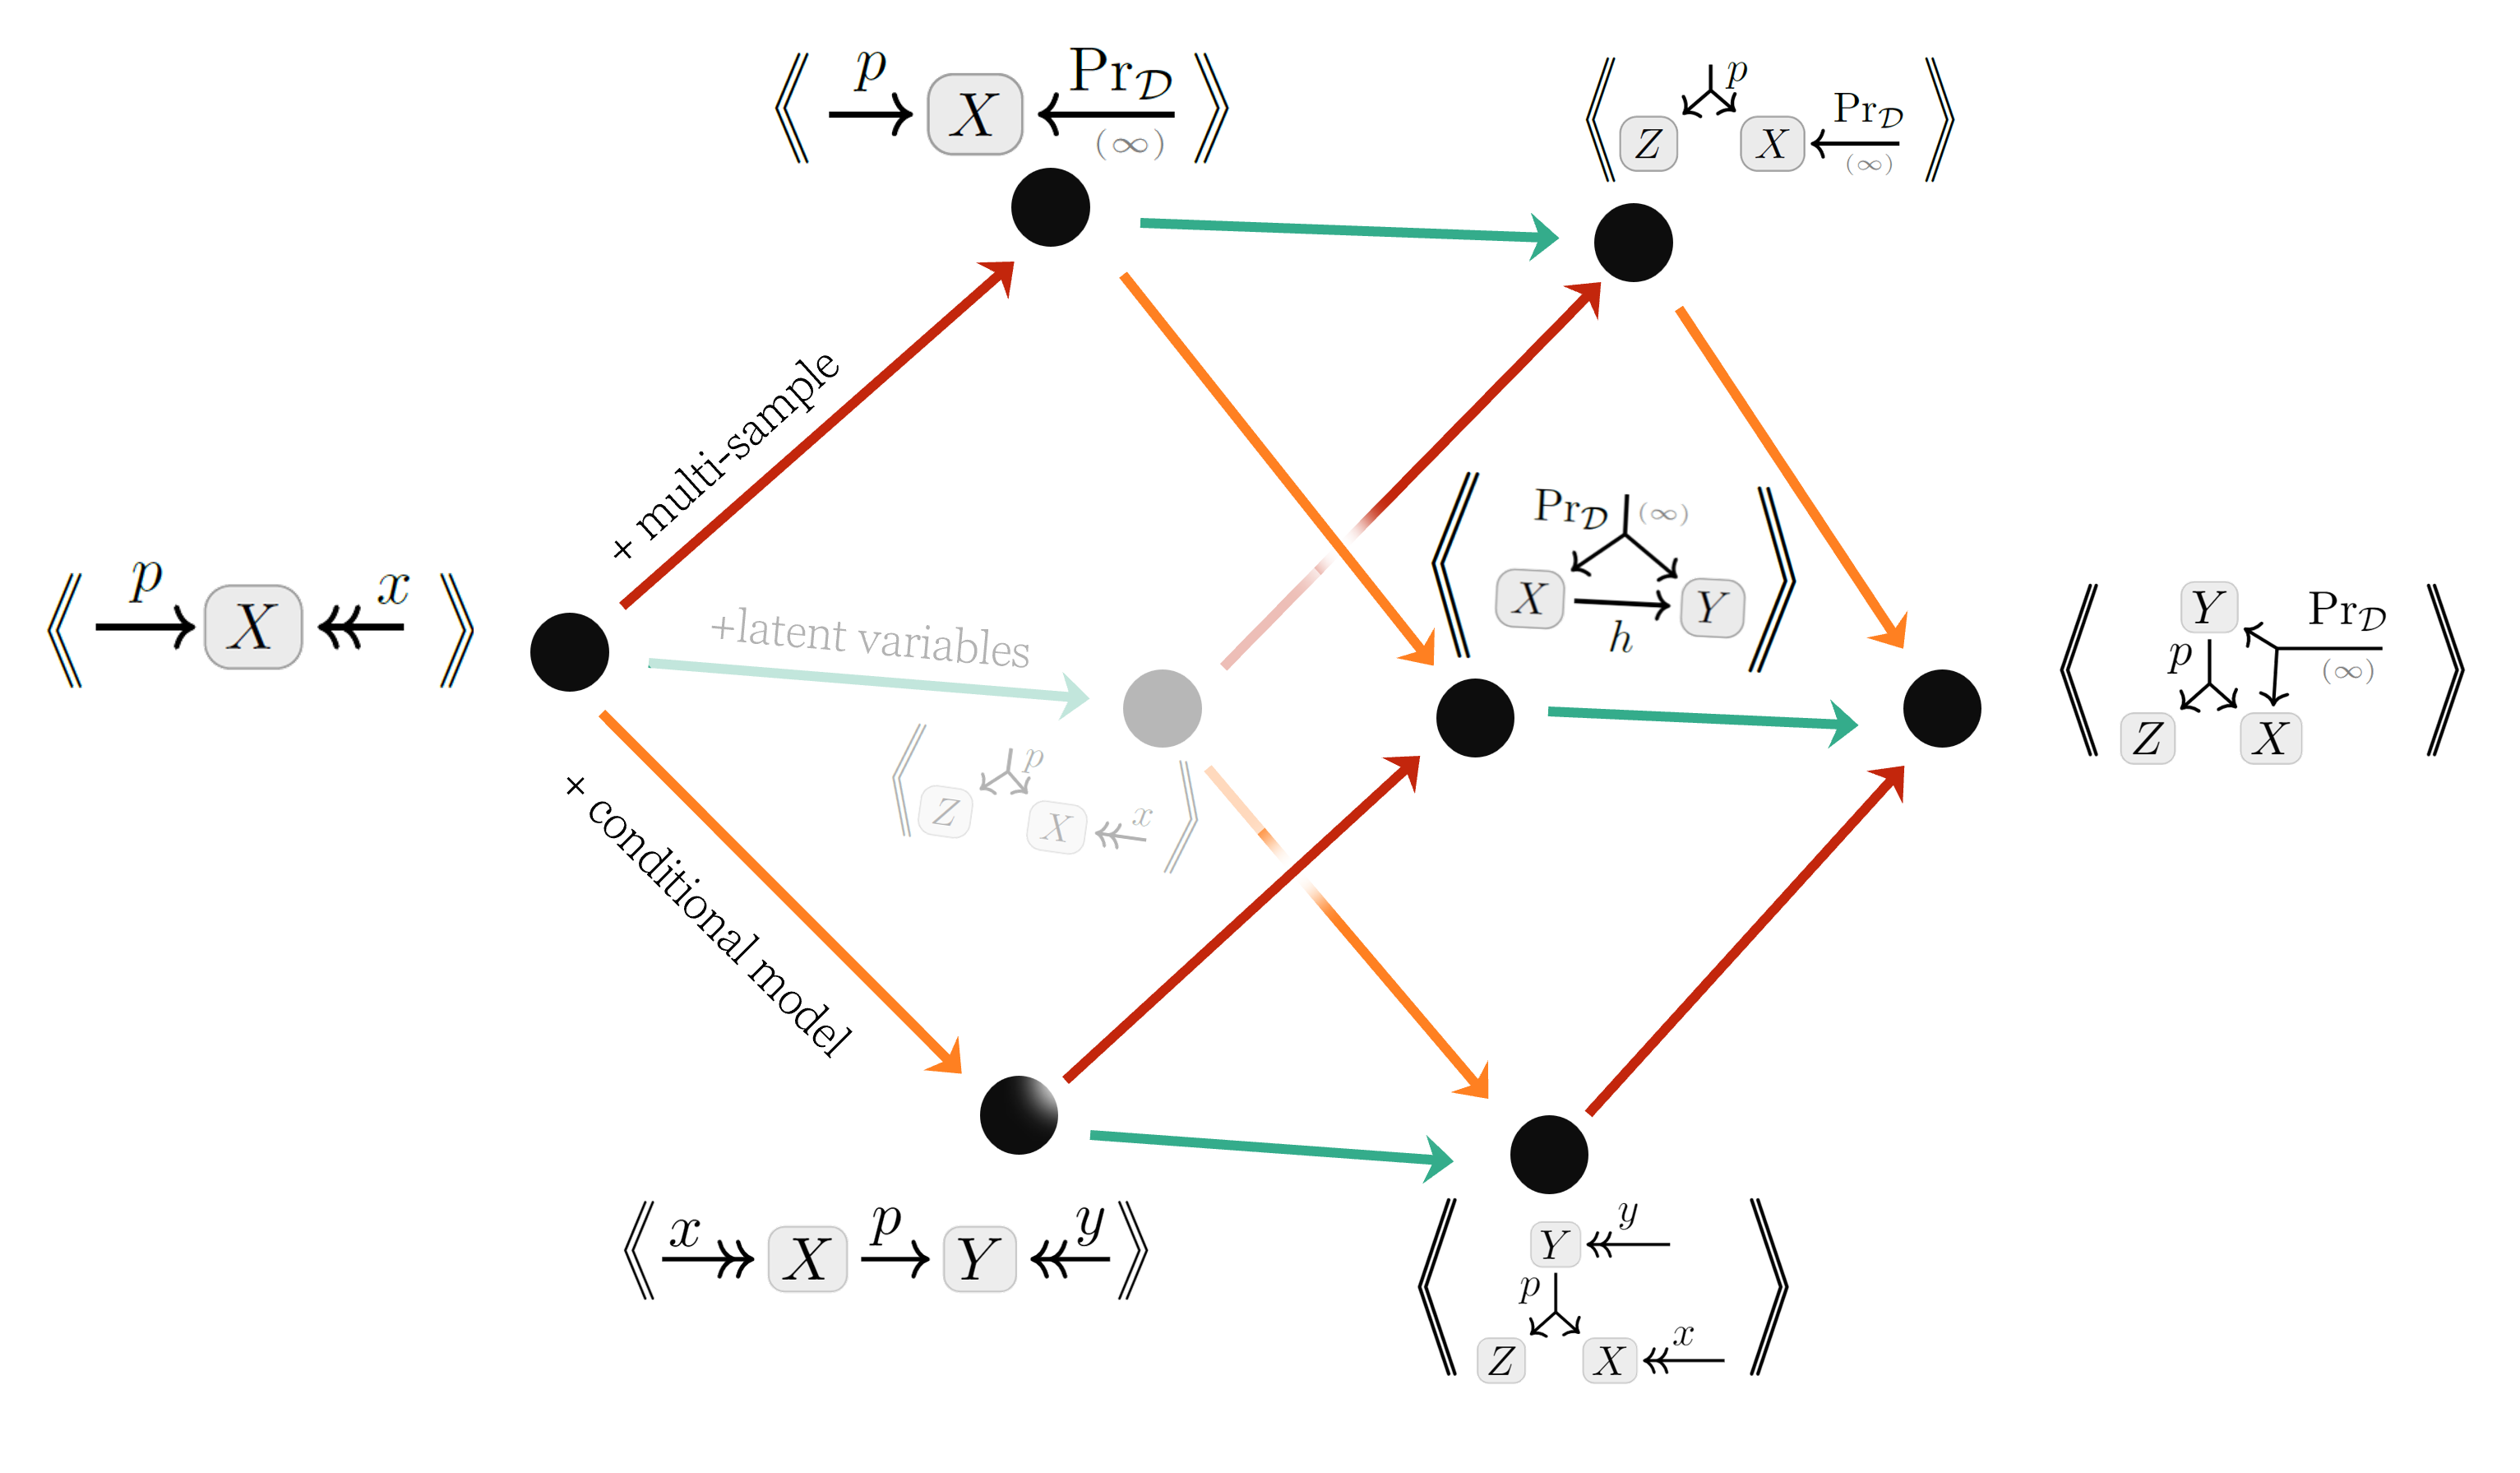
\includegraphics[width=\linewidth]{figs/entropy-cube.png}
	\caption{Variants of log-probability based losses, across three  orthogonal dimensions: conditional vs unconditional, multi-sample vs single-sample, and latent-variable vs full-information}
	\label{fig:entropy-cube}
\end{figure}

\subsection{Accuracy and Square Loss}

Simple evaluation metrics, such as the accuracy of a classifier, and the mean squared error of a regressor, also arise naturally as inconsistencies.

\begin{linked}[Log Accuracy as Inconsistency]
		{prop}{accuracy}
    Consider functions $f,h : X \!\to\! Y$ from inputs to labels, where $h$ is a predictor and $f$ generates the true labels.
    The inconsistency of believing $f$ and $h$ (with any confidences), and a distribution $D(X)$ with confidence $\beta$, is
	$\beta$ times
	the log accuracy of $h$. That is,
	% \vskip-4ex
	\begin{equation}\label{eq:accuracy-pdg}
		\aar*{\!\!\!\begin{tikzpicture}[center base]
				\node[dpad0] (Y) {$Y$};
				\node[dpad0,left=0.8 of Y] (X) {$X$};
				\draw[arr2, ->>] (X) to[bend left]
					node[pos=0.45,above right=4pt,inner sep=1pt]
						{{\color{gray}$\scriptscriptstyle(r)$}}
					node[pos=0.35, above]{$h$} (Y);
				\draw[arr2, ->>] (X) to[bend right]
					node[pos=0.45,below right=4pt,inner sep=1pt]
						{{\color{gray}$\scriptscriptstyle(s)$}}
					node[pos=0.35, below]{$f$} (Y);
				\draw[arr2, <-] (X) to
                    node[pos=0.55, anchor=south west, above]
                    {$D$}
                    node[pos=0.55, anchor=south west, below]
                    {{\color{gray}$\scriptstyle(\beta)$}}
                    +(-1.1, 0);
			\end{tikzpicture}\!}
        \begin{aligned}
		\!&=  - \beta\,\log \Pr_{x \sim D}(f(x)\!=\!h(x))  \\
		&\quad= \beta\, \I_D [f = h]. %
        \end{aligned}
	\end{equation}
\end{linked}
% \vskip-1.5ex
One often speaks of the accuracy of a hypothesis $h$, leaving the true labels $f$ and empirical distribution $D$ implicit.
Yet \Cref{prop:accuracy} suggests that there is a sense in which
$D(X)$ plays the primary role: the inconsistency in \eqref{eq:accuracy-pdg} is scaled by the confidence in $D$, and does not depend on the confidences in $h$ or $f$.
Why should this be this the case?
Expressing $(x,y)$ such that $y \ne f(x)$ with codes optimized for $f$ is not just inefficient, but impossible.
The same is true for $h$, so
we can only consider $\mu$
such that $\mu(f \!=\! h) \!=\! 1$.
In other words, the only way to form a joint distribution \emph{at all} compatible with both the predictor $h$ and the labels $f$, is to throw out samples that the predictor gets wrong---and the cost of throwing out samples scales with your confidence in $D$, not in $h$.
This illustrates why accuracy gives no gradient information for training $h$.
It is worth noting that this is precisely
the opposite of what happened in \cref{prop:supervised-cross-entropy}: there we were unwilling to budge on the input distribution, and
the inconsistency scaled with the confidence in $h$.

Observe how even properties of these simple metrics---%
relationships with one another and features of gradients%
	---can be clarified by an underlying model.






When $Y \cong \mathbb R^n$, an estimator $h(Y|X)$ is referred
to as a regressor instead of a classifier.
In this setting, most answers are incorrect, but some more so than others.
A common way of measuring incorrectness is with mean squared error (MSE):
$\Ex |f(X)-Y|^2$.
MSE is also the inconsistency of believing that
the labels and predictor have Gaussian noise---%
often a reasonable assumption because of the central limit theorem.

\begin{linked}[MSE as Inconsistency]{prop}{MSE}%
	\begin{align*}
		\aar**{\!\!\!\!\begin{tikzpicture}[center base]
			\node[dpad0] (Y) {$Y$};
			\node[dpad0,left=2.2 of Y] (X) {$X$};
			\node[dpad0,above right=0.1 and 0.7 of X] (mf) {$\mu_f$};
			\node[dpad0,below right=0.1 and 0.7 of X] (mh) {$\mu_h$};
			\draw[arr2, ->>] (X) to[bend left=0]
				node[pos=0.5, above left=0] {$f$} (mf);
			\draw[arr2, ->>] (X) to[bend right=0]
				node[pos=0.5, below left=0] {$h$} (mh);
			\draw[arr2, <-] (X) to
                node[pos=0.55, above] {$D$}
                node[pos=0.55, below]
                {{\color{gray}$\scriptstyle(\infty)$}}
                +(-1.1, 0);
			\draw[arr2, ->] (mh) to[bend right=0]
				node[pos=0.3, below right=0] {$\mathcal N_1$} (Y);
			\draw[arr2, ->] (mf) to[bend left=0]
				node[pos=0.3, above right=0]{$\mathcal N_1$} (Y);
		\end{tikzpicture}\!\!\!}
		\begin{aligned}
        = \frac12\Ex\nolimits_D \!\big| f(\mskip-1muX\mskip-1mu) - h(\mskip-1muX\mskip-1mu) \big|^2 \\
		 =: \mathrm{MSE}_D( f, h )\,,\;
        \end{aligned}
	\end{align*}
	where
    $\mathcal N_1(Y|\,\mu)$
	is a unit Gaussian on $Y$ with mean $\mu$.
\end{linked}

In the appendix, we treat general univariate
Gaussian predictors, with arbitrary variances and confidences.








\section{Regularizers and Priors as Inconsistencies}
\label{sec:regularizers}
Regularizers are extra terms added to loss functions, which provide a source of inductive bias towards simple model parameters.
There is a well-known correspondence between using a regularizer and
doing maximum \emph{a posteriori} inference with a prior
    (see \cref{appendix:MAP-and-priors}),
% \footnote{A full account can be found in the appendix.}
in which L2 regularization corresponds to a Gaussian prior
\parencite{rennie2003l2},
while L1 regularization corresponds to a Laplacian prior \parencite{williams1995bayesian}.
Note that the ability to make principled modeling choices about regularizers is a primary benefit of this correspondence.
Our approach provides a new justification of it.

\begin{linked}{prop}{regularized}
	Suppose you have a parameterized model $p(Y|\Theta)$, a prior $q(\Theta)$, and a trusted distribution $D(Y)$. The inconsistency of
	also believing $\Theta =\theta$ is the
 	cross entropy loss, plus the regularizer: $\log \frac1{q(\theta)}$ times your confidence in $q$.
	That is,
	\begin{equation}\label{eq:regularize}
		\aar*{\!\!\begin{tikzpicture}[center base]
			\node[dpad0] (theta) at (0,0) {$\Theta$};
            \node[dpad0] (Y) at (1.2,0.3) {$Y$};
			\draw[arr] (theta) --
	 			node[above]{$p$}
				(Y);
			\draw[arr2, <-] (theta) --
				node[above right=-2pt and -2pt, pos=0.7] {$q$}
				node[below left=-3pt and -4pt,pos=0.6]{{$\color{gray}\scriptstyle(\beta)$}}
				++(-1.0, 0.5);
			\draw[arr2, <<-] (theta) -- node[below,pos=0.4]{$\theta$} ++(-1.1, -0.3);
			\draw[arr2, <-] (Y) --
                node[left,pos=0.6, inner sep=2pt]{$D$}
                node[right,pos=0.6, inner sep=1pt]
                    {${\color{gray}\scriptscriptstyle(\infty)}$}
                ++(0, -0.9);
		\end{tikzpicture}\!}
		\begin{aligned}
			=\! \Ex_{y \sim D} \log \frac{1}{p(y \,|\,\theta)}
				&+ \beta \log \frac1{q(\theta)} \\[-0.2em]
	            &\!{- \H(D)} \\[-1em]
		\end{aligned}
	\end{equation}
\end{linked}

If our prior is $q(\theta) \!=\! \frac{1}{k} \exp(-\frac12 \theta^2)$%
, a (discretized) unit gaussian%
,
then the right hand side
of \eqref{eq:regularize} becomes
\[ \underbrace{\Ex\nolimits_{D}
	\log \frac{1}{p(Y \,|\, \theta)}
	}
	_{\substack{\text{Cross entropy loss}\\(\text{data-fit cost of $\theta$})}}%
	\; + \!\!\!\!\underbrace{~\frac\beta2 \theta_0~}_{\substack{\text{L2  regularizer}\\(\text{complexity cost of $\theta$})}} \!\!\!\!\!
	{\color{black} +
		\underbrace{\beta \log k - \H(D)}_{\text{constant in $p$ and $\theta$}}}\,, \]
which is the L2 regularized version of \cref{prop:expected-surprise}.
Moreover, the regularization strength corresponds exactly to the confidence $\beta$.
What about other priors? It is not difficult to see that if we use a (discretized) unit Laplacian prior, $q(\theta) \propto \exp(-|\theta|)$, the second term instead becomes $\beta |\theta_0|$, which is L1 regularization.
More generally, to consider a complexity measure $U(\theta)$, we need only include the Gibbs distribution $\Pr_U(\theta) \propto \exp(-U(\theta))$ into our PDG.
We remark that nothing here is specific to cross entropy;
any of the objectives we describe can be regularized in this way.


\section{Statistical Distances as Inconsistencies} \label{sec:statdist}

\begin{figure}
	\centering
	\def\ptradius{0.07}
    \makebox[0cm]{% flaunt margains
	% \begin{tikzpicture}[xscale=1.8, yscale=1.4]
	\begin{tikzpicture}[xscale=1.9, yscale=1.9]
        \def\rotateangle{39}

		\draw[help lines, color=gray!30, dashed] (-1.2,-1.1) grid (5.9,2.7);
		\draw[->,thick] (-1.3,0)--(6,0) node[right]{$\beta_p$};
		\draw[->,thick] (0,-1.2)--(0,2.8) node[above]{$\beta_q$} ;

		\fill[gray, fill opacity=0.2] (-1.3,1.3) -- (1.2,-1.2) -- (-1.3,-1.2) --cycle;
		\draw[gray, opacity=0.5, thick] (-1.3,1.3) --
		node[below left=0.5em and 1.5em, anchor=north, rotate=-\rotateangle,font=\footnotesize,fill=gray!20,fill opacity=0.8, inner sep=1pt, outer sep=3pt] %
			{Non-convex region} (1.2,-1.2);
		\draw[color=gray!80!orange!45, densely dashdotted] (-1, -1) -- (3,3);
		\draw[color=gray!80!orange!45, thick, <->] (1.8, 1.2) -- node[above right, anchor=south, rotate=-\rotateangle,font=\footnotesize,fill=white,fill opacity=0.8, inner sep=1pt, outer sep=3pt]{\scalebox{0.8}{Axis of Symmtry}}(1.2,1.8);


		\draw[blue!40, densely dashed, very thick, opacity=0.8]
		 	(0,1) -- node[below, align=center, pos=0.8, font=\footnotesize]{R\'enyi divergences\\for $\alpha \in (0,1)$} (5.6,1)
			(5.6,-1) -- node[above, align=center, pos=0.2, font=\footnotesize]{(negative) R\'enyi divergences\\ for $\alpha \in (1,\infty)$} (1,-1);
		\draw[red!90!blue!40, densely dashed, very thick, opacity=0.9, (-), shorten <=6pt, shorten >=6pt]
		 	(0,1) --
            node[pos=0.5,below left=3pt,anchor=north, rotate=-\rotateangle, font=\footnotesize, align=center, fill=white,fill opacity=0.8, inner sep=1pt, outer sep=2pt]
                {\scalebox{0.9}{Chernoff}}
            node[pos=0.5,below left=1.25em,anchor=north, rotate=-\rotateangle, font=\footnotesize, align=center, fill=white,fill opacity=0.8, inner sep=1pt, outer sep=2pt]{\scalebox{0.9}{Divergences}}
            (1,0);
		\draw[domain=1.6:5.6, smooth, very thick, variable=\x, blue!50!green!50, opacity=0.8, densely dashed] plot ({\x}, {1/(1-1/\x)})
			node[rotate=-7, font=\footnotesize] at (3.9,1.55){$\alpha$-divergences};

		\fill (0.5,0.5) circle (\ptradius) node[above right, align=center,
			label={[yshift=0ex,xshift=-1ex,align=left,font=\footnotesize\color{gray!50}]right:Bhattacharya\\distance}]
			{$\thickD_{B}(p,q)$};

		\fill (1,3.1) -- +(0:\ptradius) arc (0:-180:\ptradius) -- +(0:\ptradius)
			node[below]{$\vdots$}
			node[right=1ex, align=center,label={[yshift=1ex,xshift=0ex]below:\footnotesize\color{gray!50}Reverse KL}](revKL){$\kldiv qp$};

		\fill (6.4,1) -- +(270:\ptradius) arc (270:90:\ptradius) -- +(270:\ptradius)
			node[above=2pt, align=center,
				label={[yshift=-1ex,xshift=0ex]\footnotesize\color{gray!50} KL Divergence}] (FwdKL) {$\kldiv pq$}
			node[left]{$\cdots$};

		\fill (0,1) -- ++(-90:\ptradius) arc (-90:90:\ptradius)
			node[above right, align=center,
				label={[yshift=-1ex,xshift=1ex]\footnotesize\color{gray!50} Max Entropy}
			]{$\I_q(p > 0)$};

        \fill (2,-1) circle (\ptradius)
            node[above right, align=center,
                label={[yshift=-1ex,xshift=1ex, align=center,font=\footnotesize\color{gray!50}]above:$-$(Pearson)~$\chi^2$ \\[-0.1em]divergence}]
            {$-\chi^2_P\infdivx pq$};

        \fill (-1,2) circle (\ptradius)
            node[above, align=center,
                label={[yshift=-1ex,xshift=1ex, align=center,font=\footnotesize\color{gray!50}]above:$-$(Neyman)~$\chi^2$ \\[-0.1em]divergence}]
            {$-\chi^2_N\infdivx pq$};

		\fill (1,-1) -- ++(-45:\ptradius) arc (-45:135:\ptradius)
			node[above, align=center, inner sep=2pt,
				label={[yshift=-1ex,xshift=1ex]\footnotesize\color{gray!50} $-$Min Entropy}]
			{$- \log \sup \frac pq$};
	\end{tikzpicture}
    }%
	\caption[%
        Statistical distances as inconsistencies: a map of the inconsistency of $p(X)$ and $q(X)$, as their respective confidences vary.]
    {A map of the inconsistency of the PDG comprising $p(X)$ and $q(X)$, as we vary their respective confidences $\beta_p$ and $\beta_q$. Solid circles indicate well-known named measures, semicircles indicate limiting values, and the heavily dashed lines are well-established classes. }
	\label{fig:statdistmap}
\end{figure}

Suppose you are concerned with a single variable $X$. One friend has told you that it is distributed according to $p(X)$; another has told you that it follows $q(X)$. You adopt both beliefs. Your mental state will be inconsistent if (and only if) $p \ne q$, with more inconsistency the more $p$ and $q$ differ.
Thus the inconsistency of a PDG comprising $p$ and $q$ is a measure of divergence.
Recall that a PDG also allows us to specify the confidences $\beta_p$
and $\beta_q$ of each cpd, so we can form a PDG divergence
$\thickD^{\mathrm{P\mskip-2muD\mskip-1.5muG}}_{{\color{gray}(r,s)}}(p\Vert q)$
for every setting $(r,s)$ of $(\beta_p, \beta_q)$.
It turns out that a large class of statistical divergences arise in this way.
We start with a familiar one.

\begin{prop}[KL Divergence as Inconsistency]
	The inconsistency of believing $p$ with complete certainty, and also $q$ with some finite certainty $\beta$, is $\beta$ times the KL Divergence (or relative entropy) of $q$ with respect to $p$. That is,
% \vspace{-0.7em}
\[
    \aar[\Big]{\begin{tikzpicture}[center base]
        \node[dpad0] (X) {$X$};
        \draw[arr, <-] (X) --
            node[above,inner sep=2pt, pos=0.65] {$p$}
            node[below,inner sep=2pt, pos=0.65]
                {${\color{gray}\scriptscriptstyle(\infty)}$}
             ++(-1.1,0);
        \draw[arr, <-] (X) --
            node[above,pos=0.6,inner sep=2pt]
			{$q$}
			node[below,pos=0.6,inner sep=2pt]
                {$\scriptstyle{\color{gray}(\beta)}$}++(1.1, 0);
    \end{tikzpicture}}
	= \beta\, \kldiv pq .
\]
\end{prop}
% \vskip-1.3ex
This result gives us an(other) intuitive interpretation of the asymmetry of relative entropy (i.e., KL divergence), and a prescription for when it makes sense to use it.
$\kldiv p q$ is the inconsistency of a mental state containing both $p$ and $q$, when absolutely certain of $p$ (and not willing to budge on it).
This concords with the standard intuition that $\kldiv pq$ reflects the amount of information required to change $q$ into $p$, which is why
it is usually called the relative entropy ``from $q$ to $p$''.
%
We now consider the general case of a PDG comprising $p(X)$ and $q(X)$ with arbitrary confidences.
\begin{linked}{lemma}{pdgdiv}
    The inconsistency
	$\thickD^{\mathrm{P\mskip-2muD\mskip-1.5muG}}_{{\color{gray}(r,s)}}(p\Vert q)$
	of a PDG comprising $p(X)$ with confidence $r$ and $q(X)$ with confidence $s$
    is given in closed form by
	% \vspace{-1ex}
    \[
    \thickD^{\mathrm{P\mskip-2muD\mskip-1.5muG}}_{{\color{gray}(r,s)}}(p\Vert q)
    := 
        \aar[\bigg]{\begin{tikzpicture}[baseline = -0.75ex]
            \node[dpad0] (X) {$X$};
            \draw[arr2, <-] (X) --
			 		node[above, pos=0.6, inner sep=2pt, align=center] {$p$}
			 		node[below, pos=0.65, inner sep=2pt, align=center]
                        {$\scriptstyle{\color{gray}(r)}$}
				++(-1.1,0);
            \draw[arr2, <-] (X) --
			 		node[above, pos=0.6, inner sep=2pt, align=center] {$q$}
			 		node[below, pos=0.65, inner sep=2pt, align=center]
                        {$\scriptstyle{\color{gray}(s)}$}
				 ++(1.1, 0);
        \end{tikzpicture}}
        = - (r+s) \log  \sum_x \left(p(x)^{r}\vphantom{\Big|} q(x)^{s}\right)^{\frac{1}{r+s}}.
    \]
\end{linked}
% \vskip-1ex





Of the many generalizations of KL divergence, R\'enyi divergences, first characterized by Alfr\'ed R\'enyi \citeyear{renyi1961measures} are perhaps the most significant, as few others have found either application or an interpretation in terms of coding theory \parencite{van2014renyi}.
The R\'enyi divergence of order $\alpha$ between two distributions $p(X)$ and $q(X)$ is given by
% \vspace{-1ex}
\begin{equation}
	\thickD_\alpha\infdivx p q := \frac{1}{1- \alpha} \log \sum_{x \in \V(X)} p(x)^\alpha q(x)^{1-\alpha}.  \label{eq:renyi}
\end{equation}
R\'enyi introduced this measure in the same paper as the more general
class of $f$-divergences, but directs his attention towards those of
the form \eqref{eq:renyi}, because they satisfy a natural weakening of
standard postulates for Shannon entropy due to
\textcite{fadeev1957begriff}.
Concretely, every symmetric, continuous measure that additively separates over independent events, and with a certain ``mean-value property'', up to scaling,
is of the form \eqref{eq:renyi} for some $\alpha$ \parencite{renyi1961measures}.
It follows from \Cref{lemma:pdgdiv} that
every R\'enyi divergence is a PDG divergence, and
every (non-limiting) PDG divergence is a (scaled) R\'enyi divergence.

% \newpage
\begin{coro}[R\'enyi Divergences]
    For all $r,s \in \Rext$, with $r+s \ge 0$, and all $\alpha \in [0,\infty]$, we have that
	% ~\vspace{-1ex}
    \begin{align*}%
        \aar[\Big]{\!\begin{tikzpicture}[baseline = -0.75ex,scale=1.2]
            \node[dpad0] (X) {$X$};
            \draw[arr2, <-] (X) --
			 		node[above, pos=0.6, inner sep=2pt, align=center] {$p$}
			 		node[below, pos=0.65, inner sep=2pt, align=center]
                        {$\scriptstyle{\color{gray}(r)}$}
				++(-1.1,0);
            \draw[arr2, <-] (X) --
			 		node[above, pos=0.6, inner sep=2pt, align=center] {$q$}
			 		node[below, pos=0.65, inner sep=2pt, align=center]
                        {$\scriptstyle{\color{gray}(s)}$}
				 ++(1.1, 0);
        \end{tikzpicture}\!}
        % &=
        =
            s \cdot \thickD_{\frac{r}{r+s}}\infdivx{p}{q}
        % \\[-1ex]
        \qquad
        \text{and}\qquad
        \thickD_{\alpha}\infdivx{p}{q}
        % &=
        =
        \aar[\Big]{\!\begin{tikzpicture}[baseline = -0.75ex,scale=1.2]
            \node[dpad0] (X) {$X$};
            \draw[arr2, <-] (X) --
			 		node[above, pos=0.6, inner sep=2pt, align=center] {$p$}
			 		node[below, pos=0.65, inner sep=2pt, align=center]
                        {$\scriptstyle{\color{gray}(\frac{\alpha}{1-\alpha})}$}
				++(-1.3,0);
            \draw[arr2, <-] (X) --
			 		node[above, pos=0.6, inner sep=2pt, align=center] {$q$}
				 ++(0.9, 0);
        \end{tikzpicture}\!}
    \end{align*}
\end{coro}
% \vskip-1.4ex

However, the two classes are not identical, because the PDG divergences have extra limit points.
One big difference is that the reverse KL divergence $\kldiv q p$ is not a R\'enyi divergence $\thickD_\alpha\infdivx p q$ for any value (or limit) of $\alpha$.
This lack of symmetry has led others \parencite[e.g.,][]{cichocki2010families}
to work instead with a symmetric variant called $\alpha$-divergence, rescaled by an additional factor of $\frac1\alpha$.
The relationships between these quantities can be seen in \cref{fig:statdistmap}.



The Chernoff divergence measures the tightest possible exponential
bound on probability of error \parencite{nielsen2011chernoff} in Bayesian
hypothesis testing.
It also happens to be the smallest possible inconsistency of simultaneously believing $p$ and $q$, with confidences whose sum equals one.
\begin{coro}%
The Chernoff Divergence between $p$ and $q$ equals
\\[-1.8em]
\[
	\inf_{\beta \in (0,1)}
	\aar[\Big]{\begin{tikzpicture}[center base,scale=1.2]
		\node[dpad0] (X) {$X$};
		\draw[arr2, <-] (X) --
			node[above, inner sep=2pt,pos=0.6] {$p$}
			node[below, inner sep=2pt,pos=0.65] {${\color{gray}\scriptscriptstyle(\beta)}$}
			 ++(-1.1,0);
		\draw[arr2, <-] (X) --
			node[above, inner sep=2pt,pos=0.6] {$q$}
			node[below, inner sep=2pt, pos=0.65] {${\color{gray}\scriptscriptstyle(1-\beta)}$}
			++(1.1, 0);
	\end{tikzpicture}}.
\]
\end{coro}

One significant consequence of representing divergences as inconsistencies is that we can use \cref{lemma!} to derive relationships between them. The following facts follow directly from \cref{fig:statdistmap}, by inspection.
\begin{coro}
	\begin{enumerate}[nosep]
		\item R\'enyi entropy is monotonic in its parameter $\alpha$.
		\item $\kldiv p q \ge 2 \thickD_B(p,q) \le \kldiv q p$.
		\item If $q(p > 0) < 1$ (i.e., $q \not\ll p$), then $\kldiv q p = \infty$.
	\end{enumerate}
\end{coro}


These divergences correspond to PDGs with only two edges and one variable.
What about more complex graphs?
For a start, conditional divergences
% \vspace{-1.5ex}
\def\ns{\mskip-1.5mu}
\[
\thickD^{\ns\mathrm{P\mskip-2muD\mskip-1.5muG}}_{(r,s)}\ns\ns\Big(\ns p(\ns Y \ns|\ns X \ns) \ns\,\Big\Vert\,\ns q(\ns Y \ns|\ns X\ns) \ns\,\Big|\,\ns r(\ns X\ns)\!\Big)
\!:=\!\!
 \displaystyle \Ex_{x\sim r} \!\! \ns \thickD^{\ns\mathrm{P\mskip-2muD\mskip-1.5muG}}_{(r,s)}
 \ns\ns\Big(\ns
 p(\ns Y \ns|x) \ns\ns\,\Big\Vert\,\ns\ns q(\ns Y \ns|x)\!\Big)
\]
% \vskip-2ex
can be represented straightforwardly as
% \vskip-3ex
\[
\thickD^{\mathrm{P\mskip-2muD\mskip-1.5muG}}_{(r,s)}\ns(p \,\Vert\, q \,|\, r\ns)
 = \aar*{
\begin{tikzpicture}[center base]
	\node[dpad0] (X) at (0,0) {$X$};
	\node[dpad0] (Y) at (1.65,0) {$Y$};
	\draw[arr, <-] (X) --
		node[above, pos=0.55, inner sep=2pt]{$r$}
		node[below, pos=0.55, inner sep=2pt]{${\color{gray}\scriptscriptstyle(\infty)}$}
		+(-1.2,0);
	\draw[arr] (X) to[bend left=25, inner sep=1pt]
		node[above, inner sep=2pt, pos=0.35] {$p$}
		node[above, inner sep=2pt, pos=0.68]
			{${\color{gray}\scriptscriptstyle(r)}$}
		(Y);
	\draw[arr] (X)
		to[bend right=25]
		node[below, inner sep=2pt,pos=0.35] {$q$}
		node[below, inner sep=2pt, pos=0.68]
			{${\color{gray}\scriptscriptstyle(s)}$}
		(Y);
\end{tikzpicture}
}
\,.
\]
% \vskip-1ex

Other structures are useful intermediates.
\Cref{lemma!}, plus some structural manipulation, gives visual proofs of many divergence properties; \Cref{fig:dpi-vis-proof} features such a proof of the data-processing inequality.
And in general, PDG inconsistency can be viewed as a vast generalization of divergences to arbitrary structured objects.

{
% \def\pdgdiv{\thickD^{\mathrm{P\mskip-2muD\mskip-1.5muG}}_{\lgs({\color{pcolor!40}\beta},{\color{qcolor!40}\zeta})}\infdivx[\big]}
\begin{figure*}
    \colorlet{pcolor}{Plum}%
    \colorlet{qcolor}{MidnightBlue}%
	\tikzset{ci2/.style={inner sep=2pt, align=center}}%
	\def\amt{45}%
	\tikzset{pstyle/.style={line width=0.9pt, pcolor!\amt!black}}%
	\tikzset{qstyle/.style={line width=1.3pt, qcolor!\amt!black}}%
	\tikzset{pqstyle/.style={line width=1.5pt,pcolor!50!qcolor!\amt!black}}%
	\def\lgs{\color{gray!80}\scriptstyle}%
	\def\plabel{{$\lgs\color{pcolor!40}({\beta})$}}
	\def\qlabel{{$\lgs\color{qcolor!40}({\zeta})$}}
	% \scalebox{0.89}
    {{
	$
	\aar*{\!\begin{tikzpicture}[center base]
	   \node[dpad0] (X) {$X$};
	   \draw[arr2, <-,qstyle] (X) --
		  node[above,pos=0.6,ci2]{$q$}
				node[below, pos=0.65,ci2] {\qlabel}
		   ++(1.1, 0);
	   \draw[arr2, <-,pstyle] (X) --
				node[above,pos=0.6,ci2]{$p$}
				node[below, pos=0.65, ci2] {\plabel}
		   ++(-1.1, 0);%
	\end{tikzpicture}\!}
	\!=\!
	\aar**{\!\begin{tikzpicture}[center base]
	   \node[dpad0] (X) {$X$};
	   \node[dpad0,above=.9 of X,align=center] (Y) {$Y$};
	   \draw[arr2, <-,qstyle] (X) --
			node[above,pos=0.7,ci2]{$q$}
						node[below, pos=0.65,ci2] {\qlabel}
		   ++(1.1, 0);
	   \draw[arr2, <-,pstyle] (X) --
		  node[above,pos=0.7,ci2]{$p$}
						node[below, pos=0.65,ci2] {\plabel}
		   ++(-1.1, 0);%
	   \draw[arr2, pqstyle] (X) --
		  node[left,pos=0.45,inner sep=2pt]{$f$}
						node[right, pos=0.45, inner sep=1.5pt, align=center] %
							{{$\lgs\color{pcolor!50!qcolor!40}(\beta+\zeta)$}}
		  (Y);%
	\end{tikzpicture}\!}
	\!=\!
	\aar**{\!\begin{tikzpicture}[center base]
	   \node[dpad0] (X1) {$X_1$};
	   \node[dpad0, right=0.6 of X1] (X2) {$X_2$};
	   \node[dpad0,above=.8 of {$(X1)!.5!(X2)$},align=center] (Y) {$Y$};
	   \draw[arr2, -, double equal sign distance] (X1) to (X2);
	   \draw[arr2, <-,qstyle] (X2) --
		  node[above,pos=0.6,ci2]{$q$}
						node[below, pos=0.65,ci2] {\qlabel}
		  ++(1.1, 0);
	   \draw[arr2, <-,pstyle] (X1) --
		  node[above,pos=0.6,ci2]{$p$}
						node[below, pos=0.65,ci2] {\plabel}
		  ++(-1.1, 0);%
	   \draw[arr2,pstyle] (X1) to[bend left=40]
		  node[above left, pos=0.35, inner sep=1pt]{$f$}
						node[below right=0 and 0, pos=0.45, inner sep=0pt, align=center] {\plabel}
		   (Y);%
	   \draw[arr2,qstyle] (X2) to[bend right=40]
		  node[above right, pos=0.35, inner sep=1pt]{$f$}
						node[below left=0 and 0, pos=0.45, inner sep=0pt, align=center] {\qlabel}
		   (Y);%
	\end{tikzpicture}\!}
    $\\~\phantom{a}\hfill
    $
	\!\ge\!
	\aar**{\!\begin{tikzpicture}[center base]
		   \node[dpad0] (X1) {$X_1$};
		   \node[dpad0, right=0.65 of X1] (X2) {$X_2$};
		   \node[dpad0,above=.75 of {$(X1)!.5!(X2)$},align=center] (Y) {$Y$};
		   \draw[arr2, <-,qstyle] (X2) --
			  node[above,pos=0.6,ci2]{$q$}
							node[below, pos=0.65,ci2] {\qlabel}
			  ++(1.1, 0);
		   \draw[arr2, <-,pstyle] (X1) --
			  node[above,pos=0.6,pstyle,ci2]{$p$}
							node[below, pos=0.65,ci2] {\plabel}
			  ++(-1.1, 0);%
		   \draw[arr2,pstyle] (X1) to[bend left=30]
			  node[above left, pos=0.35, inner sep=1pt]{$f$}
							node[below right=0 and 0, pos=0.45, inner sep=0pt, align=center] {\plabel}
			   (Y);%
		   \draw[arr2,qstyle] (X2) to[bend right=30]
			  node[above right, pos=0.35, inner sep=1pt]{$f$}
							node[below left=0 and 0, pos=0.45, inner sep=0pt, align=center] {\qlabel}
			   (Y);%
		\end{tikzpicture}\!}
	\!=\!
	\aar*{\!\begin{tikzpicture}[center base]
	   \node[dpad0] (X) {$X$};
	   \draw[arr2, <-,qstyle] (X) --
		   node[above,pos=0.7,ci2]{$ f\!\circ\! q$}
				 node[below, pos=0.65,ci2] {\qlabel}
		   ++(1.1, 0);
	   \draw[arr2, <-,pstyle] (X) --
		   node[above,pos=0.6,ci2]{$ f\!\circ\! p$}
				 node[below, pos=0.65,ci2] {\plabel}
		   ++(-1.1, 0);%
	\end{tikzpicture}\!}
	$
	}}
    \def\pdgdiv{\thickD^{\mathrm{P\mskip-2muD\mskip-1.5muG}}_{\lgs({\color{pcolor!40}\beta},{\color{qcolor!40}\zeta})}\infdivx[\big]}
    \sbox\dpineqbox{$\pdgdiv pq \ge \pdgdiv {f\circ p}{f \circ q}$}
	\caption[A visual proof of the data-processing inequality
        for all PDG divergences, with monotonicity]{%
    A visual, monotonicity-based proof of the data-processing inequality
        for all PDG divergences:
	 	% $\pdgdiv pq \ge \pdgdiv {f\circ p}{f \circ q}$.
        % $\usebox\pdgdivbox\relax \ge $
        \usebox\dpineqbox.
	In words:
	the cpd $f(Y|X)$ can always be satisfied, so adds no inconsistency.
	It is then equivalent to split $f$ and the variable $X$ into $X_1$ and $X_2$ with edges enforcing $X_1 = X_2$.
	But removing such edges can only decrease inconsistency.
	Finally, compose the remaining cpds to give the result.
	% See the appendix for a full justification.
	See the \cref{appendix:dpi-details} for a full justification.
	}
	\label{fig:dpi-vis-proof}
\end{figure*}
}

\section{Variational Objectives and Bounds}
\label{sec:theory}


The fact that the incompatibility of $\dg M$ with a \emph{specific} joint distribution $\mu$ is an upper bound on the inconsistency is not a deep one, but it is of a variational flavor.
Here, we focus on the more surprising converse:  PDG semantics capture general aspects of variational inference.
Moreover, PDGs provide the basis of an intuitive graphical proof language for variational bounds.

\subsection{PDGs and Variational Approximations}
\label{sec:variational}
% \def\ELBO{\mathop{\mathrm{E\mskip-0.5muL\mskip-0.5muB\mskip-0.5muO}}}
\def\ELBO{\mathop{\mathrm{ELBO}}}

We begin by recounting the standard development of the `Evidence Lower BOund' (ELBO), a standard objective for training latent variable models \parencite[\S2.2]{blei2017variational}.
Suppose we have a model $p(X,Z)$, but only have access to observations of $x$.
In service of adjusting $p(X,Z)$ to make our observations more likely, we would like to maximize $\log p(X\!\!=\!x)$, the ``evidence'' of $x$ (\Cref{prop:marginal-ll}).
Unfortunately, computing $p(X) = \sum_z p(X,Z\!\!=\!z)$ requires summing over all of $Z$, which can be intractable.
The variational approach is as follows: fix a family of distributions $\mathcal Q$ that is easy to sample from, choose some $q(Z) \in \mathcal Q$, and define
$\mathrm{ELBO}_{p,q}(x) := \Ex_{z \sim q} \log \frac{p(x,z)}{q(z)}$.
This is something we can estimate, since we can sample from $q$. By Jensen's inequality,
\[
    \ELBO\limits_{p,q}(x)
    =\! \Ex_{q} \log \frac{p(x,Z)}{q(Z)}
    \le  \log \Big[\! \Ex_{q}\! \frac{p(x,Z)}{q(Z)} \Big]\!
    = \log p(x),
\]
with equality if $q(Z) = p(Z)$.
So to find $p$ maximizing $p(x)$, it suffices to adjust $p$ and $q$ to maximize $\ELBO_{p,q}(x)$,%
    \footnote{or for many iid samples: $\max_{p,q}\sum_{x \in \xsamp}\ELBO_{p,q}(x)$.}
 provided $\mathcal Q$ is expressive enough.


The formula for the ELBO is somewhat difficult to make sense of.%
\footnote{Especially if $p, q$ are densities. See \cref{appendix:density}.}
Nevertheless, it arises naturally as the inconsistency of the
appropriate PDG.

\begin{linked}{prop}{pdg-elbo-x}%
	The negative ELBO of $x$ is the inconsistency of the PDG containing $p$,$q$, and $X\!\!=\!x$, with high confidence in $q$.
	That is,
    % \vspace{-0.8em}
	\[
	-\ELBO_{p,q}(x) =
	 \aar[\Bigg]{
		\begin{tikzpicture}[center base]
			\node[dpad0] (Z) {$Z$};
			\node[dpad0,right=.5 of Z] (X) {$X$};
			\coordinate (A) at ($ (X)!.5!(Z) + (0,0.8)$);
			\draw[arr1] (A) -- node[left, inner sep=3pt]{$p$} ++(0,-0.35) -- (X);
			\draw[arr1] (A) -- ++(0,-0.35) -- (Z);
			\draw[arr2, <<-] (X) --  node[above,pos=0.8]{$ x$} ++(0.9, 0);
			\draw[arr2, <-] (Z) --
                node[above,pos=0.65, inner sep=2pt]{$q$}
                node[below,pos=0.7, inner sep=2pt]{${\color{gray}\scriptscriptstyle(\infty)}$}
                ++(-0.9, 0);%
		\end{tikzpicture}
		}%
		.
	\]
\end{linked}
% \vskip-1ex



Owing to its structure, a PDG is often more intuitive and easier to work with than the formula for its inconsistency.
To illustrate,
we now give a simple and visually intuitive proof of the bound traditionally used to motivate the ELBO, via \cref{lemma!}:
\[
\log  \frac{1}{p(x)} =
	 \aar*{
		\begin{tikzpicture}[center base,scale=1.2]
			\node[dpad0] (Z) {$Z$};
			\node[dpad0,right=.5 of Z] (X) {$X$};
			\coordinate (A) at ($ (X)!.5!(Z) + (0,0.7)$);
			\draw[arr1] (A) -- node[left, inner sep=2pt]{$p$} ++(0,-0.25) -- (X);
			\draw[arr1] (A) -- ++(0,-0.25) -- (Z);
			\draw[arr2, <<-] (X) --  node[left,pos=0.8]{$x$} ++(0.2, 0.8);
		\end{tikzpicture}
        ~
		}%
	\le
	 \aar*{
		\begin{tikzpicture}[center base,scale=1.2]
			\node[dpad0] (Z) {$Z$};
			\node[dpad0,right=.5 of Z] (X) {$X$};
			\coordinate (A) at ($ (X)!.5!(Z) + (0,0.7)$);
            \draw[arr1] (A) -- node[left, inner sep=2pt]{$p$} ++(0,-0.25) -- (X);
			\draw[arr1] (A) -- ++(0,-0.25) -- (Z);
            \draw[arr2, <<-] (X) --  node[left,pos=0.8]{$x$} ++(0.2, 0.8);
			\draw[arr2, <-] (Z) -- node[left, inner sep=2pt,pos=0.5]{$q$}
                node[above, inner sep=1.5pt, rotate=-70, pos=0.7]{{${\color{gray}\scriptscriptstyle(\infty)}$}}
                ++(110:0.9);
		\end{tikzpicture}
        ~
		}%
    = - \ELBO_{p,q}(x).
\]

The first and last equalities are \Cref{prop:marginal-ll,prop:pdg-elbo-x} respectively.
Now to reap some pedagogical benefits.
The second PDG has more edges so it is clearly at least as inconsistent. Furthermore, it's easy to see that equality holds when $q(Z) \!=\! p(Z)$: the best distribution for the left PDG has marginal $p(Z)$ anyway, so insisting on it incurs no further cost.




\subsection{Variational Auto-Encoders and PDGs}

An autoencoder is a probabilistic model intended to compress a
variable $X$ (e.g., an image) to a compact latent representation
$Z$.
Its structure is given by two conditional distributions:
an encoder $e(Z | X)$, and a decoder $d(X | Z)$.
Of course, not all pairs of cpds fill this role equally well.
One important consideration is the
\emph{reconstruction error} \eqref{eq:rec}: when we decode an encoded image, we would like it to resemble the original.
% \vspace{-0.5em}
\begin{equation}
	\mathrm{Rec}(x) := \!\!\!\!\! \Ex_{z \sim e(Z|x)} \smash{\underbrace{\mathrm I_{d(X |z)}(x)\vphantom{\Big|}}_{\mathclap{\left(\;\substack{\text{additional bits required to}\\\text{decode $x$ from its encoding  $z$}}\;\right)}}}
	= \sum_z e(z \,|\, x) \log \frac1{d(x \,|\, z)}\label{eq:rec}
\end{equation}
% \vspace{0.0ex}
\medskip

There are other desiderata as well. Perhaps good latent representations $Z$ have uncorrelated components, and are normally distributed.
We encode such wishful thinking as a belief $p(Z)$, known as a variational prior.

The data of a Variational Auto-Encoder
\parencite{kingma2013autoencoding,rezende2014stochastic}, or VAE,
consists of $e(Z|X)$, $d(X|Z)$, and $p(Z)$.
The encoder $e(Z|X)$ can be used as a variational approximation of $Z$, differing from $q(Z)$ of \Cref{sec:variational} only in that it can depend on $X$.
VAEs are trained with the analogous form of the ELBO:
\begin{align*}
	\mathrm{ELBO}_{p,e,d}(x) :=&
		\Ex_{z \sim e(Z|x)} \left[\log \frac{p(z) d(x\mid z)}{e(z\mid x)} \right] \\
		=& - \mathrm{Rec}(x) - \kldiv{e(Z|x)}{p}.
\end{align*}
% \vspace{-3ex}

This gives us the following analog of \cref{prop:pdg-elbo-x}.

\begin{linked}{prop}{pdg-elbo-vae}
	The VAE loss of a sample $x$
    is the inconsistency of the PDG comprising the encoder
	$e$
	(with high confidence, as it defines the encoding),
	decoder
	$d$, prior $p$, and $x$.
	That is,
    % \vspace{-3ex}
	\[
	-\mathrm{ELBO}_{p,e,d}(x) =
	 \aar*{
		\begin{tikzpicture}[center base]
			\node[dpad0] (Z) {$Z$};
			\node[dpad0,right=.7 of Z] (X) {$X$};
			\draw[arr2, ->] (X) to[bend left=50]
				node[above, inner sep=2pt]{$e$}
				node[below, inner sep=2pt]{${\color{gray}\scriptscriptstyle(\infty)}$}
                (Z);
			\draw[arr2, ->] (Z) to[bend left=50]
				node[above]{$ d$} (X);
			\draw[arr2, <<-] (X) --
			  	node[above,pos=0.8]{$ x$}
			 	++(0.9, 0);
			\draw[arr2, <-] (Z) --
				node[above,pos=0.6]{$ p$}
				++(-0.9, 0);%
		\end{tikzpicture}}.
 	\]
    % \vspace{-4ex}
\end{linked}


We now give a visual proof of the analogous variational bound.
Let $\Pr_{p,d}(X,Z) := p(Z)d(X|Z)$ be
the distribution that arises from decoding the prior. Then:
\begin{align*}
	\log \frac{1}{\displaystyle\mathop{\mathrm{P\mkern-1.5mur}}_{p\mkern-1mu,d}(\mskip-1.5mux\mskip-1.5mu)} =
	\aar**
	{\begin{tikzpicture}
			[baseline=1.9ex,scale=1.2]
		\node[dpad0] (Z) {$Z$};
		\node[dpad0,right=.4 of Z] (X) {$X$};
		\draw[arr2, ->] (Z) to[bend left=50,looseness=1.5]
			node[above]{$\smash{d}$} (X);
		\draw[arr2, <<-] (X) --
			node[left,pos=0.8,inner sep=2pt]{$x$} ++(0.2, 0.8);
		\draw[arr2, <-] (Z) --
			node[right,pos=0.7,inner sep=2pt]{$p$} ++(-0.2, 0.8);%
	\end{tikzpicture}}
	&\le
	\aar**
	{\begin{tikzpicture}
		[baseline=1.5ex,scale=1.2]
		\node[dpad0] (Z) {$Z$};
		\node[dpad0,right=.7 of Z] (X) {$X$};
		\draw[arr2, ->] (X) to[bend left=0]
			node[above, inner sep=2pt]{$e$}
			node[below, inner sep=1pt, pos=0.4]
				{${\color{gray}\scriptscriptstyle(\!\infty\!)}$}
			(Z);
		\draw[arr2, ->] (Z) to[bend left=50,looseness=1.5]
			node[above, inner sep=2pt]{$\smash{d}$} (X);
		\draw[arr2, <<-] (X) --
			node[left,pos=0.8,inner sep=2pt]{$x$} ++(0.2, 0.8);
		\draw[arr2, <-] (Z) --
			node[right,pos=0.7,inner sep=2pt]{$p$} ++(-0.2, 0.8);%
   \end{tikzpicture}}
   = \shortminus\ELBO\limits_{p,e,d}(x).
\end{align*}

The first and last equalities are \Cref{prop:marginal-ll,prop:pdg-elbo-vae}, and the inequality is \cref{lemma!}.
See the appendix for multi-sample analogs of the bound and \cref{prop:pdg-elbo-vae}.

\subsection{The \texorpdfstring{$\beta$}{beta}-VAE Objective}
\label{sec:betavae}

The ELBO is not the only objective that has been used to train networks with a VAE structure.
In the most common variant, due to \textcite{higgins2016beta},
one weights the reconstruction error \eqref{eq:rec} and
the `KL term' differently, resulting in a loss function of the form
% \vspace{-0.5ex}
\[
	\beta\text{-}\mathrm{ELBO}_{p,e,d}(x) := - \mathrm{Rec}(x) - \beta \kldiv{e(Z|x)}{p},
\]
% \vskip-1.5ex
which, when $\beta \!=\! 1$, is the ELBO as before. The authors view $\beta$ as a regularization strength, and argue that
it sometimes helps to have a stronger prior.
Sure enough:
% \vspace{-2ex}
\begin{linked}{prop}{betaelbo-informal}
\!\!$-\beta\text{-ELBO}_{p,e,d}(x)$ is the inconsistency of
the same PDG,
but with confidence $\beta$ in $p(Z)$.%
\end{linked}


\section{Free Energy as Factor Graph Inconsistency}
    \label{sec:free-energy-fg-inc}
A weighted factor graph $\Psi = (\phi_J, \theta_J)_{J \in \cal J}$, where each $\theta_J$ is a real-valued weight, $J$ is associated with a subset of variables $\mathbf X_J$, and  $\phi_J : \V(\mathbf X_J) \to \mathbb R$, determines a distribution by
% \vskip-1.4em
\vspace{-2ex}
\[
	\Pr\nolimits_\Psi(\mat x) = \frac{1}{Z_\Psi} \prod_{J \in \cal J} \phi_J(\mat x_J)^{\theta_J}.
\]
% \vskip-0.7em
\(
	Z_{\Psi} %
\)
is the constant
$ \sum_{\mat x} \prod_{J \in \mathcal J} \phi_J(\mat x_J)^{\theta_J}$
required to normalize the distribution,
and is known as the \emph{partition function}. Computing $\log Z_\Psi$
is intimately related to probabilistic inference in factor graphs \parencite{ma2013estimating}.
We will revisit this point in \cref{chap:inc-infer-connection}.
Following \textcite{pdg-aaai},
let $\PDGof{\Psi}$ be the PDG with edges $\{ \raisebox{-0.3ex}{$\smash{\stackrel{J}{\rightarrow}}$} \mathbf X_J \}_{\mathcal J}$, cpds $p_J(\mathbf X_J) \propto \phi_J(\mathbf X_J)$, and weights
$\alpha_J, \beta_J := \theta_J$%
. There, it is shown that
$\Pr_\Psi$ is the unique minimizer of $\bbr{\PDGof{\Psi}}_1$.
But what about the corresponding inconsistency, $\aar{\PDGof{\Psi}}_1$?

If the factors are normalized and all variables are edge targets,
then $Z_\Psi \le 1$,
so $\log \frac{1}{Z_\Psi} \ge 0$
measures how far the product of factors is from being a probability distribution.
So in a sense, it measures $\Psi$'s inconsistency.

\begin{linked}{prop}{fg-inconsistency-is-partition-function}
	For all weighted factor graphs
	$\Psi$,
	 we have that $\aar{\PDGof{\Psi}}_1 = - \log Z_{\Psi}$.
\end{linked}

The exponential families generated by weighted factor graphs
are a cornerstone of statistical mechanics, where $- \log Z_{\Psi}$ is known as the (Heimholz) free energy.
It is also an especially natural quantity to minimize:
the principle of
free-energy minimization has been enormously successful in describing
of not only chemical and biological systems \parencite{chipot2007free}, but also cognitive ones \parencite{friston2009free}.

\section{Beyond Standard Losses: A Concrete Example}
	\label{sec:datsim}
In contexts where a loss function is standard, it is usually for good reason---which is why we have focused on recovering standard losses.
But most situations are non-standard, and even if they have standard sub-components, those components may interact with one another in more than one way.
Correspondingly, there is generally more than one way to cobble standard loss functions together.
How should you choose between them?
By giving a principled model of the situation.

\def\simsymb{\texttt{s\kern-1.1pti\kern-0.8ptm}}
\def\datsymb{\texttt{d\kern-0.75pta\kern-1ptt}}
\def\ssymb{\texttt{s}}
\def\dsymb{\texttt{d}}
Suppose we want to train a predictor network $h(Y|X)$ from two sources of information:
partially corrupted data with distribution $d(X,Y)$,
and a simulation with distribution $s(X,Y)$.
If the simulation is excellent and the data unsalvageable, we would have high confidence in $s$ and low confidence in $d$,
in which case we would train with cross entropy with respect to $s$%
, $\mathcal L_{\simsymb}\!:=\!\Ex_s [\log \nf1{h(Y|X)}]$.
Conversely, if the simulation were bad and the data mostly intact, we would use
$\mathcal L_\datsymb$,
the cross entropy with respect to $d$.
What if we're not so confident in either?

One approach a practitioner might find attractive is to make a dataset from samples of both $s$ and $d$%
, or equivalently, train with a convex combination
of the two previous losses,
$\mathcal L_1 := \lambda_{\ssymb}\mathcal L_{\simsymb} + \lambda_{\dsymb}\mathcal L_{\datsymb}$
for some $\lambda_\ssymb, \lambda_\dsymb > 0$ with $\lambda_\ssymb + \lambda_\dsymb = 1$.
This amounts to training $h$ with cross entropy with respect to the mixture
$\lambda_\ssymb s + \lambda_\dsymb d$
	(\ref{claim:6.7.1} in the appendix).
Doing so treats $d$ and $s$ as completely unrelated, and so redundancy is not used to correct errors---a fact on display when we present the modeling choices in PDG form,
such as
% \vspace{-1ex}
\[
\mathcal L_1 = \aar**{
\begin{tikzpicture}[center base]
	\node[tpt={z0|\simsymb}] at (-1.5,0.1) {};
	\node[tpt={z1|\datsymb},right=0.35 of z0]{};
	\node[Dom={$Z$[label distance=-2.5ex, xshift=1.0em] (Z)
		around {\lab{z0}\lab{z1}}},yshift=0.2em ] {};

	\node[dpad0] (X) at (2.4, 0.6) {$X$};
	\node[dpad0] (Y) at (2.4, -0.6) {$Y$};
	\coordinate (xyz) at (1.9, 0);
	\draw[arr1, <-] (Z) to
		node[above, pos=0.6]{$\lambda$}
		node[below,inner sep=1pt, pos=0.6]{${\color{gray}\scriptstyle( \infty )}$}
		+(-1.8, 0);
	\draw[arr1] (X) to node[right,pos=0.4]{$h$} (Y);
	\draw[arr,-,shorten >=0pt] (Z) to [bend left=0, shorten >=0pt]
		node[above, inner sep=1pt, pos=0.55]
		{$\begin{matrix}\datsymb \mapsto d \\[-0.6ex]
			\simsymb \mapsto s \end{matrix}$}
		node[below,inner sep=1pt]{${\color{gray}\scriptstyle( \infty )}$}
		(xyz);
	\draw[arr2, shorten <=0pt] (xyz) to (X);
	\draw[arr2, shorten <=0pt] (xyz) to (Y);
\end{tikzpicture}%
}
	,
\]
in which a switch variable $Z$
with possible values
$
\{\simsymb,\datsymb\}$
controls whether samples come from $s$ or $d$, and
is distributed according to
$\lambda(Z\!=\!\simsymb) = \lambda_\ssymb$.


Our practitioner now tries a different approach: draw data samples $(x,y) \sim d$ but discount $h$'s surprisal when the simulator finds the point unlikely, via loss $\mathcal L_2 := \Ex_{d} [s(\mkern-2muX\!,\!Y\mkern-2mu) \log \nf1{h(Y|X)}]$.
This is the cross entropy with respect to the (unnormalized) product density $ds$, which in many ways is appropriate.
However, by this metric, the optimal predictor is $h^*(Y|x) \propto d(Y|x) s(Y|x)$,
which is
\emph{uncalibrated} \parencite{dawid1982well}.
If the data and simulator agree ($d \!=\! s$), then we would want $h(Y|x) \!=\! s(Y|x)$ for all $x$, but instead we get $h^*(Y|x) \propto s(Y|x)^2$.
So $h^*$ is overconfident.
What went wrong?
$\mathcal L_2$ cannot be written as the (ordinary $\gamma\!=\!0$) inconsistency
of a PDG containing only $s,h$, and $d$,
but for a large fixed $\gamma$, it is essentially the $\gamma$-inconsistency
\[
\mathcal L_2 \approx
C
\aar**{
\begin{tikzpicture}[center base]
	\node[dpad0] (X) at (0, 0.6) {$X$};
	\node[dpad0] (Y) at (0, -0.6) {$Y$};
	\draw[arr1] (X) to node[left, pos=0.4, inner sep=1pt]{$h$} (Y);

	\coordinate (d0) at (1.8, 0);
	\coordinate (dmid) at (0.9, 0);
	\coordinate (s0) at (-1.8, 0);
	\coordinate (smid) at (-0.9, 0);

	\draw[arr,->,shorten <=0pt] (dmid) to[bend right=25] (X);
	\draw[arr,->,shorten <=0pt] (dmid) to[bend left=25] (Y);
	\draw[arr1,-,shorten <=0pt] (dmid) to
		node[below, inner sep=2pt]{${\color{gray}\scriptstyle
			\renewcommand{\arraystretch}{.7}
			\big(\begin{matrix}
				\scriptstyle\alpha: 1 \\[-0.2ex] \scriptstyle\beta: \gamma
			\end{matrix} \big)}$}
		node[above] {$d$}
		(d0);
	\draw[arr,->,shorten <=0pt] (smid) to[bend left=25] (X);
	\draw[arr,->,shorten <=0pt] (smid) to[bend right=25] (Y);
	\draw[arr1,-,shorten <=0pt] (smid) to
		node[below, inner sep=2pt]{${\color{gray}\scriptstyle
			\renewcommand{\arraystretch}{.7}
			\big( \begin{matrix}
				\scriptstyle \alpha: 1 \\[-0.2ex] \scriptstyle \beta: \gamma
			\end{matrix} \big)}$}
		node[above]{$s$}
		(s0);
\end{tikzpicture}}\Bigg._{\!\!\!\gamma}
 + \mathit{const},
\]
where $C$ is the constant required to normalize the joint density $sd$, and $\mathit{const}$ does not depend on $h$ (\ref{claim:6.7.2}).
However, the values of $\balpha$ in
this PDG indicate an over-determination of $XY$
(it is determined in two different ways),
  and so $h^*$ is more deterministic than intended.
  	\label{ex:overdet2}
By contrast,
% \vspace{-2ex}
\[
\mathcal L_3 := \aar**{
\begin{tikzpicture}[center base]
	\node[dpad0] (X) at (0, 0.6) {$X$};
	\node[dpad0] (Y) at (0, -0.6) {$Y$};
	\draw[arr1] (X) to node[left=0pt,pos=0.4, inner sep=1pt]{$h$} (Y);


	\coordinate (d0) at (1.8, 0);
	\coordinate (dmid) at (0.9, 0);
	\coordinate (s0) at (-1.8, 0);
	\coordinate (smid) at (-0.9, 0);

	\draw[arr,->,shorten <=0pt] (dmid) to[bend right=25] (X);
	\draw[arr,->,shorten <=0pt] (dmid) to[bend left=25] (Y);
	\draw[arr1,-,shorten <=0pt] (dmid) to
		node[below, inner sep=2pt]{${\color{gray}\scriptstyle(\lambda_{\dsymb})}$}
		node[above] {$d$}
		(d0);
	\draw[arr,->,shorten <=0pt] (smid) to[bend left=25] (X);
	\draw[arr,->,shorten <=0pt] (smid) to[bend right=25] (Y);
	\draw[arr1,-,shorten <=0pt] (smid) to
		node[below, inner sep=2pt]{${\color{gray}\scriptstyle(\lambda_{\ssymb})}$}
		node[above]{$s$}
		(s0);
\end{tikzpicture}},
\]
does not have this issue: the optimal predictor $h^*$
 according to $\mathcal L_3$
 is proportional to the $\lambda$-weighted geometric mean of $s$ and $d$ (\ref{claim:6.7.3}).
It seems that our approach, in addition to providing a unified view of standard loss functions, can also suggest more appropriate loss functions in practical situations.

\section{Reverse-Engineering a Loss Function?}
	\label{sec:reverse-engineer}

% \def\Tru{{\tt T}}
% \def\trut{{\tt t}}
% \def\truf{{\tt f}}

Given an \emph{arbitrary} loss function, can we find a PDG that gives rise to it?
The answer,
	\newmaterial{as we discovered in \cref{sec:soft-constraint-widget}, }
	appears to be yes---although not without making unsavory modeling choices.
Without affecting its semantics, one may add the variable $\Tru$ that takes values $\{\trut, \truf\}$, and the event $\Tru \!\!=\! \trut$, to any PDG.
Now, given a
cost function $c: \V(X) \to \mathbb R_{\ge 0}$,
define the cpd $\hat c(\Tru |X)$ by
$
	\hat c(\trut | x) := e^{-c(x)}.
$
By threatening to generate the falsehood {\truf} with probability dependent on the cost of $X$, $\hat c$ ties the value of $X$ to inconsistency.
\begin{linked}{prop}{expected-cost}
	\!
	\( \displaystyle
		\aar*{\!\begin{tikzpicture}[center base]
			\node[dpad0] (X) at (0,0) {$X$};
			\node[dpad0] (2) at (1.1,0) {$\Tru$};

			\draw[arr2] (X) to
				node[above, pos=0.4,inner sep=2pt]{$\hat c$}
				(2);
			\draw[arr2, <-] (X) to
				node[above, pos=0.6, inner sep=2pt]{$p$}
				node[below, pos=0.6, inner sep=2pt]
					{${\color{gray}\scriptscriptstyle(\mskip-2mu\infty\mskip-2mu)}$}
				+(-1, 0);
			\draw[arr2, <<-] (2) to
				node[above, inner sep=2pt, pos=0.6]
					{\trut}
				+(0.9,0);
		\end{tikzpicture}\!}
	 	= \!
		\Ex_{x\sim p}\!    [\,c(x)\,].
	\)
\end{linked}
Setting confidence $\beta_p := \infty$ may not be realistic since
we're still training the model $p$,
but doing so is necessary to recover $\Ex_p c$.%
\footnote{If $\beta_p$ were instead equal to $1$, we would have obtained $-\log \Ex_p \exp(-c(\!X\!))$, with optimal distribution $\mu(\!X\!) \!\ne\! p(\!X\!)$ (\hyperref[claim:6.8.1]{Claim 6.8.1} in the appendix).\label{fn:logEexp}}
Any mechanism that generates inconsistency based on the value of $X$ (such as this one) also works in reverse:
the PDG ``squirms'', contorting the probability of $X$ to disperse the inconsistency.
One cannot cannot simply ``emit loss''
without affecting the rest of the model,
as one does
with utility
in an Influence Diagram \parencite{influencediagrams}.
Even setting every $\beta := \infty$ may not be enough to prevent the squirming.
\def\mypdg{\dg{S}}
To illustrate, consider a model $\mypdg$ of the supervised learning setting (predict $Y$ from $X$), with labeled data $\mathcal D$, model $h$, and a loss function $\ell$ on pairs of output labels.

Concretely, define:
% \vspace{-1ex}
\[
	\mypdg
	:=
	\begin{tikzpicture}[baseline=4ex]
		\begin{scope}[xscale=1.4]
			\node[dpad0] (X) at (0.3,0) {$X$};
			\node[dpad0] (Yt) at (1,1) {$Y$};
			\node[dpad0,align=center] (Yp) at (1.4,0) {$\vphantom{Y}\smash{Y'}$};
			\node[dpad0] (2) at (2,1) {$\Tru$};

			\coordinate (dstart) at (-0.1,0.9);
		\end{scope}

		\unmergearr[arr1]{dstart}{X}{Yt}
			\node[above=2pt of center-dstartXYt, xshift=-2pt] {$\datadist\xysamp$};
			\node[below right=2.0pt and -0.4pt of center-dstartXYt, inner sep=0pt, rotate=25]
				{${\color{gray}\scriptscriptstyle(\mskip-2mu\infty\mskip-2mu)}$};

		\mergearr[arr2]{Yt}{Yp}{2}
			\node[above=2pt of center-YtYp2] {$\hat\ell$};

		\draw[arr2] (X) to
			node[above, inner sep=2pt,pos=0.4] {$h$}
			node[below, inner sep=2pt,pos=0.4]
				{${\color{gray}\scriptscriptstyle(\mskip-2mu\infty\mskip-2mu)}$}
			(Yp);
		\draw[arr2, <<-] (2) to
			node[right, inner sep=2pt, pos=0.6]
				{\trut}
			+(0,-1);
	\end{tikzpicture}
	\qquad\;\text{and}\;\qquad
	\mathcal L := \;\;\mathop{\scalebox{1.2}{$\Ex$}}\limits_{\substack{%
		\vphantom{x}\\
		\mathllap{(x,y)} \sim \mathrlap{\datadist\xysamp} \\
		\mathllap{y'} \sim \mathrlap{p(Y'|\,x)}} }
	 \;\big[\ell(y,y')\big].
	 % \vspace{-1.5ex}
\]

Given \Cref{prop:expected-cost},
one might imagine $\aar{\mypdg} = \mathcal L$,
but this is not so.
In some ways, $\aar{\mypdg}$ is actually preferable.
The optimal $h(Y'|X)$ according to $\mathcal L$ is
a degenerate cpd that places all mass on the label(s) $y^*_X$ minimizing expected loss,
while the optimal $h(Y'|X)$ according to $\aar{\mypdg}$ is $\datadist\xysamp(Y|X)$,
which means that it is calibrated, unlike $\ell$.
If, in addition, we set $\alpha_p, \alpha_{\datadist\xysamp} := 1$ and
strictly enforce the qualitative picture,
finally no more squirming is possible, as we arrive at
$\displaystyle\lim_{\gamma\to\infty}\aar{\mypdg}_\gamma = \mathcal L$
(\hyperref[claim:6.8.2]{Claim 6.8.2}).
% \vskip-0.5ex

In the process, we have given up our ability to tolerate inconsistency by setting all probabilistic modeling choices in stone.
What's more, we've dragged in the global parameter $\gamma$,
further handicapping our ability to compose this model with others.
To summarize: while model inconsistency readily generates appropriate loss functions,
the converse does not work as well.
Reverse-engineering a loss may require making questionable modeling choices with absolute
certainty, resulting in brittle models with limited potential for composition.
In the end, we must confront our modeling choices;
good loss functions come from good models.



\section{Conclusions}


We seen that that PDG semantics 
%\unskip, in the same stroke by which they 
not only capture Bayesian Networks and Factor Graphs \parencite{pdg-aaai}, but also generate
many standard loss functions, including some non-trivial ones.
In each case, the appropriate loss arises simply by articulating modeling assumptions, and then measuring inconsistency.
Viewing loss functions in this way also has beneficial side effects, including an intuitive visual proof language for reasoning about the relationships between them.

This ``universal loss'',
which provides a principled way of choosing an optimization objective,
may be of particular interest to the AI alignment community.


% \newpage


\clearpage
\begin{subappendices}

\section{Notes}
% \subsection{The Fine Print for Probability Densities}
% \subsection{The Fine Print for Probability Densities}
\paragraph{The Fine Print for Probability Densities.}
\label{appendix:density}
% \textbf{Densities and Masses.} Many of our results (%
Several of our results (%
\Cref{prop:pdg-Ix,%
	prop:expected-surprise,%
	prop:marginal-ll,%
	prop:pdg-loglikelihood,%
	prop:many-equal-simple,%
	prop:supervised-cross-entropy,%
	prop:pdg-elbo-x,%
	prop:pdg-elbo-vae,%
	prop:pdg-elbo-vae-whole%
})
technically require the distribution to be represented with a mass function (as opposed to a probability density function, or pdf).
A PDG containing both pdf and a finitely supported distribution on the same variable
will typically have infinite inconsistency---%
but this is not just a quirk of the PDG formalism.


Probability density is not dimensionless (like probability mass), but rather has inverse $X$-units (e.g., probability per meter), so depends on an arbitrary choice of scale (the pdf for probability per meter and per centimeter will yield different numbers).
In places where the objective does not have units that cancel before we take a logarithm,
the use of a probability density $p(X)$ becomes sensitive to this arbitrary choice of parameterization. For instance, the analog of surprisal, $- \log p(x)$ for a pdf $p$, or its expectation, called differential entropy, both depend on an underlying scheme of measurement (an implicit base measure).

On the other hand, this choice of scale ultimately amounts to an additive constant.
Moreover, beyond a certain point, decreasing the discretization size $k$ of a discretized approximation $\tilde p_k(X)$ \emph{also} contributes a constant that depends only on $k$.
But such constants are irrelevant for optimization, and so, even though such quantities are ill-defined and arguably meaningless in the continuous limit, the use of the continuous analogs as loss functions is still justified.

The bottom line is that all our results hold in a uniform way for every discretization size --- yet in the limit as the discretization becomes smaller, an inconsistency may diverge to infinity.
However, this divergence stems from an additive constant that depends only on the discretization size, which is irrelevant to its employment as a loss function.
As a result, using one of these ``unbalanced'' functions involving densities where the units do not work out properly, results in a morally equivalent loss function, except without a diverging constant.
\newmaterial{%
This is a direct analogue of our discussion of entropy for continuous variables (\cref{sec:prelim-gen-ent}). 
}%

\commentout{%
\textbf{Markov Kernels.} In the more general setting of measurable spaces, one may want to adjust the definition of a cpd that we gave, so that one instead works with \emph{Markov Kernels}.
This imposes an additional constraint: suppose the variable $Y$ takes values in the measurable space $(\V(Y), \mathcal B)$. If $p(Y|X)$ is to be a \emph{Markov Kernel}, then for every fixed measurable subset $B \in \mathcal B$ of the measure space, the we must require that  $x \mapsto \Pr(B|x)$ be a measurable function (with respect to the measure space in which $X$ takes values).
This too mostly does not bear on the present discussion, because the $\sigma$-algebras for all measure spaces of interest, are fine enough that one can get an arbitrarily close approximation of any cpd with a Markov Kernels.
This means that the infimum defining the inconsistency of a PDG does not change.
}%s

% \subsection{Maximum A Posteriori (MAP) updating, Priors, and Regularization}
\paragraph{Maximum A Posteriori (MAP) updating, Priors, and Regularization.}
    \label{appendix:MAP-and-priors}

The usual telling of the correspondence between regularizers and priors is something like the following.
Suppose you have a parameterized family of distributions
$\Pr(X|\Theta)$
and have observed evidence $X$, but do not know the parameter $\Theta$.
The maximum-likelihood estimate of $\Theta$ is then
\[
	\theta^{\mathrm{MLE}}(X) := \arg\max_{\theta\in \Theta}~  \Pr(X \mid \theta)
		= \arg\max_{\theta\in \Theta} ~ \log \Pr(X \mid \theta).
\]
The logarithm is a monotonic transformation, so it does not change the argmax, but it has
nicer properties, so that function is generally used instead. (Many of the loss functions in main body of the paper are log-likelihoods also.)

In some sense, better than estimating the maximum likelihood, is to perform a Bayesian update with the new information, to get a \emph{distribution} over $\Theta$.
If that's too expensive, we could simply take the estimate with the highest posterior probability, which is called the Maximum A Posteriori (MAP) estimate.
For any given $\theta$, the Bayesian reading of Bayes rule states that
\[
	\text{posterior $\Pr(\Theta | X)$} = \frac
		{\text{likelihood $\Pr(X|\Theta)$}\cdot\text{prior $\Pr(\Theta)$}}{\text{evidence $\Pr(X) = \sum_{\theta'} \Pr(X|\theta')\Pr(\theta')$}}.
\]
So taking a logarithm,
\[
    \def\parcenterss#1{\parbox{3cm}{\centering\singlespacing #1}}
    %
	\parcenterss{log-posterior\\ $\log \Pr(\Theta | X)$} 
    = \parcenterss{log-likelihood \\ $\log \Pr(X|\Theta)$}
     ~+~ \parcenterss{log-prior\\ $\log \Pr(\Theta)$}
		- \parcenterss{log-evidence\\ $\log \Pr(X)$}.
\]
The final term does not depend on $\theta$, so it is not relevant for finding the optimal $\theta$ by this metric. Swapping the signs so that we are taking a minimum rather than a maximum, the MAP estimate is then given by
\[
 	\theta^{\mathrm{MAP}}(X) := \arg\min_{\theta \in \Theta} \left\{ \log \frac{1}{\Pr(X|\theta)} + \log \frac1{\Pr(\theta)} \right\}.
\]
Note that if negative log likelihood (or surprisal, $-\log \Pr(X|\theta)$) was our original loss function, we have now added an arbitrary extra term, as a function of $\Theta$, to our loss function. It is in this sense that priors classically correspond to regularizers.

\section{Further Results and Generalizations}
\subsection{Full Characterization of Gaussian Predictors}
The inconsistency of a PDG containing two univariate Gaussian regressors of with arbitrary parameters and confidences, is most cleanly articulated in terms of the geometric and quadratic means.

\begin{defn}[Weighted Power Mean]
	The weighted power mean $\mathrm M^w_p(\mathbf r)$ of the collection of real numbers $\mathbf r = r_1, \ldots, r_n$ with respect to the convex weights $w = w_1, \ldots, w_n$ satisfying $\sum_iw_i = 1$, is given by
	\[
		\mathrm M^w_p(\mathbf r) := \Big(\sum_{i=1}^n w_i (r_i)^p \Big)^{\frac1p}.
	\]
	We omit the superscript as a shorthand for the uniform weighting $w_i = \nicefrac{1}{N}$.
\end{defn}

\begin{table}
\centering
\renewcommand{\arraystretch}{1.5} %
\begin{tabular}{rcl}
	\textbf{Name} & $p$ & \textbf{Formula}\\\hline
	Harmonic&$(p=-1)$:& $\mathrm{HM}_w(\mathbf r) = \faktor1{\left(\sum_{i=1}^n \nicefrac{w_i}{r_i}\right)}$ \\
	Geometric&$(\lim {p\to 0})$:& $\mathrm{GM}_w(\mathbf r) = \prod_{i=1}^n r_i^{w_i}$ \\
	Arithmetic&$(p=1)$:& $\mathrm{AM}_w(\mathbf r) = \sum_{i=1}^n w_i r_i$ \\
	Quadratic&$(p=2)$:& $\mathrm{QM}_w(\mathbf r) = \sqrt{\textstyle\sum_{i=1}^n w_i r_i^2}$\\\hline
	\end{tabular}
	\caption{special cases of the $p$-power mean $\mathrm M_p^w(\mathbf r)$}
	\label{tab:power-means}
\end{table}

Many standard means, such as those in \cref{tab:power-means}, are special cases.
It is well known that $\mathrm M_p^w(\mathbf r)$ is increasing in $p$, and strictly so if not all elements of $\mathbf r$ are identical. In particular, $\mathrm{QM}_w(a,b) > \mathrm{GM}_w(a,b)$ for all $a \ne b$ and positive weights $w$. We now present the result.

\newpage
\begin{linked}{prop}{inc-two-gaussians}
	Consider a PDG containing two (distinct) conditional Gaussian distributions on a variable $Y$, whose parameters can both depend on a variable $X$. Its inconsistency takes the form
	\begin{align*}
		&\aar**{\!\!\!\!\begin{tikzpicture}[center base]
			\node[dpad0] (Y) {$Y$};
			\node[dpad0,left=2.4 of Y] (X) {$X$};
			\node[dpad0,above right=0.6 and 0.8 of X] (mf) {$\mu_1$};
			\node[dpad0,below right=0.6 and 0.8 of X] (mh) {$\mu_2$};
			\node[dpad0,above right=0.1 and 0.8 of X] (sf) {$\sigma_1$};
			\node[dpad0,below right=0.1 and 0.8 of X] (sh) {$\sigma_2$};
			\draw[arr2, ->>] (X) to[bend left=30]
				node[pos=0.6, inner sep=0.2pt, fill=white, fill opacity=0.9] {$f$} (mf);
				\draw[arr2, ->>] (X) to[bend left=10]
					node[pos=0.4, inner sep=0.2pt, fill=white, fill opacity=0.9] {$s$} (sf);
			\draw[arr2, ->>] (X) to[bend right=30]
					node[pos=0.6, inner sep=0.2pt, fill=white, fill opacity=0.9] {$h$} (mh);
				\draw[arr2, ->>] (X) to[bend right=10]
					node[pos=0.4, inner sep=0.2pt, fill=white, fill opacity=0.9] {$t$} (sh);
			\draw[arr2, <-] (X) to
				node[pos=0.55, above]{$D$}
				node[below,pos=0.55, inner sep=2pt]
					{${\color{gray}\scriptscriptstyle(\infty)}$}
				+(-1.1, 0);
			\coordinate (C1) at ($(mf)!.5!(sf) + (0.85,-0.2)$);
			\coordinate (C2) at ($(mh)!.5!(sh) + (0.85,+0.2)$);
			\draw[arr2, ->] (mh) to[bend right=15] (C2) to[out=45,in=-160]
				node[pos=0.25, below right, inner sep=0]
					{${\mathcal N}$}
				node[pos=0,below=6pt,inner sep=1pt] {$\scriptstyle{\color{gray}(\beta_2)}$}
				(Y);
			\draw[arr2, -,shorten >=0pt] (sh) to[bend right=25] (C2);
			\draw[arr2, ->] (mf) to[bend left=15] (C1) to[out=-45,in=160]
				node[pos=0.25, above right, inner sep=1pt]
					{${\mathcal N}$}
				node[pos=0,above=6pt,inner sep=1pt] {$\scriptstyle{\color{gray}(\beta_1)}$}
				(Y);
			\draw[arr2, -,shorten >=0pt] (sf) to[bend left=25] (C1);
		\end{tikzpicture}\!} %
		 \\&=
			\Ex_{D}\left[
    			(\beta_1 \!+\! \beta_2) \log \frac
    				{ \mathrm{QM}_{\hat\beta}(\sigma_1,\sigma_2) }
    				{ \mathrm{GM}_{\hat\beta}(\sigma_1,\sigma_2) }
    			+ \frac12 \frac{\beta_1\beta_2}{\beta_1+\beta_2} \left(\frac{\mu_1- \mu_2}{ \mathrm{QM}_{\hat\beta}(\sigma_1,\sigma_2)}\right)^{\!2} \right]
		 \numberthis\label{eq:2gaussians} \\
		 % &\hspace{-2cm}
		 &= \frac12 \Ex_{x \sim D} \left[
		 	\frac{\beta_1 \beta_2}2
		 	\frac{\Big(f(x) - h(x)\Big)^2}
		 		{\beta_2 s(x)^2 + \beta_1 t(x)^2}
			+ \frac{\beta_1 + \beta_2}{2}
				\log \frac
				{\beta_2 s(x)^2 + \beta_1 t(x)^2 }
				{\beta_1 + \beta_2}
			\begin{array}{l} - \beta_2 \log s(x)\\ - \beta_1 \log t(x) \end{array}
		 \right]
	\end{align*}
	where  $\hat\beta = (\frac{\beta_2}{\beta_1+\beta_2}, \frac{\beta_1}{\beta_1+\beta_2})$ represents the normalized and reversed vector of confidences $\beta = (\beta_1, \beta_2)$ for the two distributions, and $\mu_1 = f(X)$, $\mu_2 = g(X)$, $\sigma_1 = s(X)$, $\sigma_2 = t(X)$ are random variables over $X$.
\end{linked}



The PDG on the left is semantically equivalent to (and in particular has the same inconsistency as) the PDG
\[
\begin{tikzpicture}[center base]
	\node[dpad0] (Y) {$Y$};
	\node[dpad0,left=1.1 of Y] (X) {$X$};
	\draw[arr2, ->] (X) to[bend left]
		node[pos=0.5, above] {$\mathcal N(f(x), s(x))$} (Y);
	\draw[arr2, ->] (X) to[bend right] node[pos=0.5, below]{$\mathcal N(h(x), t(x))$} (Y);
	\draw[arr2, <-] (X) to
		node[pos=0.6, above]{$D$}
		node[below,pos=0.6, inner sep=2pt]
			{${\color{gray}\scriptscriptstyle(\infty)}$}
		+(-1.1, 0);
\end{tikzpicture}
.
\]
This illustrates an orthogonal point: that PDGs handle composition of functions as one would expect, so that it is equivalent to model an entire process as a single arrow, or to break it into stages, ascribing an arrow to each stage, with one step of randomization.

As a bonus, \cref{prop:inc-two-gaussians} also gives a proof of the inequality of the weighted geometric and quadratic means.
\begin{coro} For all $\sigma_1$ and $\sigma_2$, and all weight vectors $\beta$,
	$
	{\mathrm {QM}_{\hat\beta}(\sigma_1,\sigma_2)} \ge {\mathrm {GM}_{\hat\beta}(\sigma_1,\sigma_2)}.
	$
\end{coro}

\subsection{Full-Dataset ELBO and Bounds}

We now present the promised multi-sample analogs from \cref{sec:variational}.



\begin{linked}{prop}{pdg-elbo-vae-whole}
	The following analog of \cref{prop:pdg-elbo-vae} for a whole dataset $\xsamp$ holds:
	\[
	-\Ex_{\datadist\xsamp}\mathrm{ELBO}_{p,e,d}(X) =
	 \aar*{
		\begin{tikzpicture}[center base]
			\node[dpad0] (Z) {$Z$};
			\node[dpad0,right=.7 of Z] (X) {$X$};
			\draw[arr2, ->] (X) to[bend left=50,looseness=1.2]
				node[below]{$e$}
				node[above,pos=0.45, inner sep=2pt]
					{${\color{gray}\scriptscriptstyle(\infty)}$}
				(Z);
			\draw[arr2, ->] (Z) to[bend left=50]
				node[above]{$d$} (X);
			\draw[arr2, <-] (X) --
				node[above,pos=0.6]{$\datadist\xsamp$}
				node[below,pos=0.6, inner sep=2pt]
					{${\color{gray}\scriptscriptstyle(\infty)}$}
				++(1.2, 0);
			\draw[arr2, <-] (Z) --
				node[above,pos=0.6]{$p$}
				++(-0.9, 0);%
		\end{tikzpicture}} + \H(\datadist\xsamp). \]
\end{linked}

\Cref{prop:expected-surprise,prop:pdg-elbo-vae-whole} then give us an analog of the visual bounds in the body of the main paper (\cref{sec:variational}) for many i.i.d. data points at once, with only a single application of the inequality:
\begin{align*}
	- \log \Pr(\xsamp) = - \log \prod_{i=1}^m \left(\Pr(x^{(i)})\right) &=
	- \frac1{m}\sum_{i = 1}^m \log \Pr(x^{(i)})   = \\
	= \H(\datadist\xsamp) + \aar*{\begin{tikzpicture}[center base]
	   \node[dpad0] (Z) {$Z$};
	   \node[dpad0,right=0.8 of Z] (X) {$X$};
	   \draw[arr2, ->] (Z) to[bend left=30]
		   node[above]{$d$} (X);
	   \draw[arr2, <-] (X) --
		   node[above,pos=0.6]{$\datadist\xsamp$}
		   node[below,pos=0.6, inner sep=2pt]
			   {${\color{gray}\scriptscriptstyle(\infty)}$}
		   ++(1.1, 0);
	   \draw[arr2, <-] (Z) --
		   node[above,pos=0.6]{$p$}
		   ++(-0.9, 0);%
	\end{tikzpicture}}
 	&\le
 	\aar*{\begin{tikzpicture}[center base]
		\node[dpad0] (Z) {$Z$};
		\node[dpad0,right=.8 of Z] (X) {$X$};
		\draw[arr2, ->] (X) to[bend left=50]
			node[below]{$e$}
			node[above,pos=0.45, inner sep=2pt]
				{${\color{gray}\scriptscriptstyle(\infty)}$}
			(Z);
		\draw[arr2, ->] (Z) to[bend left=50, looseness=1.1]
			node[above]{$d$} (X);
		\draw[arr2, <-] (X) --
			node[above,pos=0.6]{$\datadist\xsamp$}
			node[below,pos=0.6, inner sep=2pt]
				{${\color{gray}\scriptscriptstyle(\infty)}$}
			++(1.1, 0);
		\draw[arr2, <-] (Z) --
			node[above,pos=0.6]{$ p$}
			++(-0.9, 0);%
	\end{tikzpicture}} + \H(\datadist\xsamp) \\
	&\qquad\qquad= -\Ex_{\datadist\xsamp}\mathop{\mathrm{ELBO}}\limits_{p,e,d}(X)
\end{align*}


We also have the following formal statement of \Cref{prop:betaelbo-informal}.
\begin{linked}{prop}{beta-elbo}
	The negative $\beta$-ELBO objective for a prior $p(X)$, encoder $e(Z \mid X)$, decoder $d(X \mid Z)$, at a sample $x$, is equal to the inconsistency of the corresponding PDG, where the prior has confidence equal to $\beta$. That is,
	\[
	-\beta\text{-}\mathrm{ELBO}_{p,e,d}(x) =
	 \aar**{
		\begin{tikzpicture}[center base]
			\node[dpad0] (Z) {$Z$};
			\node[dpad0,right=.7 of Z] (X) {$X$};
			\draw[arr2, ->] (X) to[bend left=50,looseness=1.2]
				node[below]{$ e$}
				node[above,pos=0.45, inner sep=2pt]
					{${\color{gray}\scriptscriptstyle(\infty)}$}
					 (Z);
			\draw[arr2, ->] (Z) to[bend left=50]
				node[above]{$ d$} (X);
			\draw[arr2, <<-] (X) --
			  	node[above,pos=0.8]{$ x$}
			 	++(0.9, 0);
			\draw[arr2, <-] (Z) --
				node[above,pos=0.55]{$p$}
				node[below,pos=0.55, inner sep=2pt]
					{${\color{gray}\scriptstyle(\beta)}$}
				++(-1.1, 0);%
		\end{tikzpicture}}
	\]
\end{linked}
As a specific case (i.e., effectively by setting $\beta_p := 0$), we get the reconstruction error as the inconsistency of an autoencoder (without a variational prior):
\begin{coro}[reconstruction error as inconsistency]
\[
-\mathrm{Rec}_{ed,d}(x) :=
	\Ex_{z \sim e(Z|x)} \I_{d(X|z)}(x) =
 \aar**{
	\begin{tikzpicture}[center base]
		\node[dpad0] (Z) {$Z$};
		\node[dpad0,right=.7 of Z] (X) {$X$};
		\draw[arr2, ->] (X) to[bend left=50]
			node[below]{$ e$}
			node[above,pos=0.45, inner sep=2pt]
					{${\color{gray}\scriptscriptstyle(\infty)}$}
			(Z);
		\draw[arr2, ->] (Z) to[bend left=50]
			node[above]{$ d$} (X);
		\draw[arr2, <<-] (X) --
			node[above,pos=0.8]{$ x$}
			++(0.9, 0);
	\end{tikzpicture}}
\]
\end{coro}

\subsection{More Variants of Log Likelihood Results} \label{appendix:more-crossent}

First, we show that our cross entropy results hold for all $\gamma$, in the sense that $\gamma$ contributes only a constant.

\begin{linked}{prop}{many-equal-simple}
	Given a model determining a probability distribution with mass function $p(X)$, and samples $\xsamp = \{ x_i \}_{i=1}^m$ determining an empirical distribution $\datadist\xsamp$,  the following are equal, for all $\gamma \ge 0$:
	\begin{enumerate}
	\item The average negative log likelihood $\ell(p; \xsamp) = - \frac{1}{m} \sum_{i=1}^m \log p(x_i)$
	\item The cross entropy of $p$ relative to $\datadist\xsamp$
	\item $\bbr{\,p\,}_\gamma(\datadist\xsamp) ~{\color{gray}~+ (1+\gamma)\H(\datadist\xsamp)}$ \\[-1.4em]
	\item \(\aar[\Big] {
		\begin{tikzpicture}[center base]
			\node[dpad0] (X) {$X$};
			\coordinate (A) at ($(X) + (-0.9,0)$);
			\draw[arr1] (A) -- node[above]{$p$}  (X);
			\draw[arr2, <-] (X) --
				node[above,pos=0.6]{${\datadist\xsamp}$}
				node[below,pos=0.6, inner sep=2pt]
					{${\color{gray}\scriptscriptstyle(\infty)}$}
				++(1.2, 0);
		\end{tikzpicture}
		}_\gamma
		~{\color{gray}~+ (1+\gamma) \H(\datadist\xsamp)}
		\)
\end{enumerate}
\end{linked}

As promised, we now give the simultaneous generalization of the surprisal result
	(\Cref{prop:pdg-Ix}) to both multiple samples (like in \Cref{prop:expected-surprise}) and partial observations (as in \Cref{prop:marginal-ll}).

\begin{linked}{prop}{pdg-loglikelihood}
	The average \emph{marginal} negative log likelihood $\ell(p;x) := -\frac{1}{|\xsamp|}\sum_{x \in \xsamp} \log \sum_z p(x,z)$ is the inconsistency of the PDG containing $p$ and the data distribution $\datadist\xsamp$, plus the entropy of the data distribution (which is constant in $p$).
	That is,
	\[
	\ell(p;\xsamp) =
	 \aar[\Bigg]{
		\begin{tikzpicture}[center base]
			\node[dpad0] (Z) {$Z$};
			\node[dpad0,right=.5 of Z] (X) {$X$};
			\coordinate (A) at ($ (X)!.5!(Z) + (0,0.7)$);
			\draw[arr1] (A) -- node[right]{$p$} ++(0,-0.25) -- (X);
			\draw[arr1] (A) -- ++(0,-0.25) -- (Z);
			\draw[arr1, <-] (X) --
				node[above,pos=0.65] {$\datadist\xsamp$}
				node[below,pos=0.65, inner sep=2pt]
					{${\color{gray}\scriptscriptstyle(\infty)}$}
				++(1.1, 0);
		\end{tikzpicture}
		}%
		+ \H(\datadist\xsamp).
	\]
\end{linked}

% \clearpage
%\begin{append}

\section{Proofs}\label{loss-appendix:proofs}
\allowdisplaybreaks

{\renewcommand\footnote[1]{}\recall{lemma:!}}
\begin{lproof}
	\label{proof:!}
	For every $\mu$, adding more edges only adds non-negative terms to \eqref{eq:oinc1}, while	increasing $\beta$ results in larger coefficients on the existing (non-negative) terms of \eqref{eq:oinc1}. So for every fixed distribution $\mu$, we have
	$\bbr{\dg M}_\gamma(\mu) \le \bbr{\dg M'}_\gamma(\mu)$. So it must also be the case that the infimum over $\mu$, so we find that
	$\aar{\dg M} \le \aar{\dg M'}$.
\end{lproof}

\recall{prop:pdg-Ix}
\begin{lproof}\label{proof:pdg-Ix}
	Any distribution $\mu(X)$ that places mass on some $x' \ne x$ will have infinite KL divergence from the point mass on $x$. Thus, the only possibility for a finite consistency arises when $\mu = \delta_x$, and so
	\begin{equation*}
		\aar[\Big] {
		\begin{tikzpicture}[center base]
			\node[dpad0] (X) {$X$};
			\coordinate (A) at ($(X) + (-0.9,0)$);
			\draw[arr1] (A) -- node[above]{$ p$}  (X);
			\draw[arr2, <<-] (X) --  node[above,pos=0.8]{$ x$} ++(0.9, 0);
		\end{tikzpicture}
		}
		= \bbr*{\begin{tikzpicture}[center base]
			\node[dpad0] (X) {$X$};
			\coordinate (A) at ($(X) + (-0.9,0)$);
			\draw[arr1] (A) -- node[above]{$ p$}  (X);
			\draw[arr2, <<-] (X) --  node[above,pos=0.8]{$ x$} ++(0.9, 0);
		\end{tikzpicture}}( \delta_x )
		= \kldiv{\delta_x}{p} = \log \frac{1}{p(x)} = \I_p(x).
	\end{equation*}
\end{lproof}


\Cref{prop:many-equal-simple} is a generalization of \Cref{prop:expected-surprise}, so we prove them at the same time.
\recall{prop:expected-surprise}
\recall{prop:many-equal-simple}
\begin{lproof} \label{proof:many-equal-simple}\label{proof:expected-surprise}
	The equality of 1 and 2 is standard. The equality of 3 and 4 can be seen by the fact that in the limit of infinite confidence on $\datadist\xsamp$, the optimal distribution must also equal $\datadist\xsamp$, so the least inconsistency is attained at this value.
	Finally it remains to show that the first two and last two are equal:
	\begin{align*}
		\bbr{\,p\,}_\gamma(\datadist\xsamp) + (1+\gamma)\H(\datadist\xsamp)
		&=  \kldiv{\datadist\xsamp}{p} - \gamma \H(\datadist\xsamp)+ (1+\gamma)\H(\datadist\xsamp) \\
		&= \kldiv{\datadist\xsamp}{p} + \H(\datadist\xsamp) \\
		&= \Ex\nolimits_{\datadist\xsamp}\left[\log\frac{\datadist\xsamp}{p} +  \log\frac{1}{\datadist\xsamp}\right]
		= \Ex\nolimits_{\datadist\xsamp}\left[\log\frac{1}{p}\right],
	\end{align*}
	which is the cross entropy, as desired.
\end{lproof}


\recall{prop:marginal-ll}
\begin{lproof}\label{proof:marginal-ll}
	As before, all mass of $\mu$ must be on $x$ for it to have a finite score.
	Thus it suffices to consider joint distributions of the form $\mu(X,Z) = \delta_x(X) \mu(Z)$.
	We have
	\begin{align*}
	\aar*{
		\begin{tikzpicture}[center base]
			\node[dpad0] (Z) {$Z$};
			\node[dpad0,right=.5 of Z] (X) {$X$};
			\coordinate (A) at ($ (X)!.5!(Z) + (0,0.7)$);
			\draw[arr1] (A) -- node[right]{$ p$} ++(0,-0.25) -- (X);
			\draw[arr1] (A) -- ++(0,-0.25) -- (Z);
			\draw[arr2, <<-] (X) --  node[above,pos=0.8]{$ x$} ++(0.9, 0);
		\end{tikzpicture}}
			&= \inf_{\mu(Z)} \bbr*{\begin{tikzpicture}[center base]
				\node[dpad0] (Z) {$Z$};
				\node[dpad0,right=.5 of Z] (X) {$X$};
				\coordinate (A) at ($ (X)!.5!(Z) + (0,0.7)$);
				\draw[arr1] (A) -- node[right]{$ p$} ++(0,-0.25) -- (X);
				\draw[arr1] (A) -- ++(0,-0.25) -- (Z);
				\draw[arr2, <<-] (X) --  node[above,pos=0.8]{$ x$} ++(0.9, 0);
			\end{tikzpicture}}\Big(\delta_x(X)\mu(Z)\Big)  \\
			&= \inf_{\mu(Z)}\kldiv[\Big]{\delta_x(X)\mu(Z)}{p(X,Z)} \\
			&= \inf_{\mu(Z)}\Ex_{z \sim \mu} \log \frac{\mu(z)}{p(x,z)}
			~= \inf_{\mu(Z)}\Ex_{z \sim \mu} \log \frac{\mu(z)}{p(x,z)}\frac{p(x)}{p(x)} \\
			&= \inf_{\mu(Z)}\Ex_{z \sim \mu} \left[ \log \frac{\mu(z)}{p(z \mid x)} + \log \frac{1}{p(x)} \right] \\
			&= \inf_{\mu(Z)} \Big[\kldiv{\mu(Z)}{p(Z\mid x)}\Big] + \log \frac{1}{p(x)} \\
			&= \log \frac{1}{p(x)} = \I_p(x) & \text{[Gibbs Inequality]}
	\end{align*}
\end{lproof}



\recall{prop:pdg-loglikelihood}
\begin{lproof}\label{proof:pdg-loglikelihood}
	The same idea as in \cref{prop:marginal-ll}, but a little more complicated.
    %
	\begin{align*}
	\aar*{
		\begin{tikzpicture}[center base]
			\node[dpad0] (Z) {$Z$};
			\node[dpad0,right=.5 of Z] (X) {$X$};
			\coordinate (A) at ($ (X)!.5!(Z) + (0,0.7)$);
			\draw[arr1] (A) -- node[right]{$p$} ++(0,-0.25) -- (X);
			\draw[arr1] (A) -- ++(0,-0.25) -- (Z);
			\draw[arr2, <<-] (X) --  node[above,pos=0.8]{$\datadist\xsamp!$} ++(0.9, 0);
		\end{tikzpicture}}
			&= \inf_{\mu(Z \mid X)} \bbr*{\begin{tikzpicture}[center base]
				\node[dpad0] (Z) {$Z$};
				\node[dpad0,right=.5 of Z] (X) {$X$};
				\coordinate (A) at ($ (X)!.5!(Z) + (0,0.7)$);
				\draw[arr1] (A) -- node[right]{$ p$} ++(0,-0.25) -- (X);
				\draw[arr1] (A) -- ++(0,-0.25) -- (Z);
				\draw[arr2, <<-] (X) --  node[above,pos=0.8]{$ \datadist\xsamp!$} ++(0.9, 0);
			\end{tikzpicture}}\Big(\datadist\xsamp(X) \mu(Z \mid X)\Big)  \\
			&= \inf_{\mu(Z \mid X)}\kldiv[\Big]{\datadist\xsamp(X) \mu(Z \mid X)}{p(X,Z)} \\
			&= \inf_{\mu(Z \mid X)}
				\Ex_{\substack{x \sim \datadist\xsamp \\ z \sim \mu}}
					\log \frac{\mu(z \mid x)\datadist\xsamp(x)}{p(x,z)} \\
			&= \frac{1}{|\xsamp|}\inf_{\mu(Z\mid X)}\sum_{x \in \xsamp}
				\Ex_{z \sim \mu(Z\mid x)} \log \frac{\mu(z \mid x) \datadist\xsamp(x) }{p(x,z)}\frac{p(x)}{p(x)} \\
			&= \frac{1}{|\xsamp|}\inf_{\mu(Z \mid X)}\sum_{x \in \xsamp}
				\left[ \Ex_{z \sim \mu}
				\left[ \log \frac{\mu(z\mid x)}{p(z \mid x)}  \right] + \log \frac{1}{p(x)}
				- \log \frac{1}{\datadist\xsamp(x)}  \right] \\
			&= \frac{1}{|\xsamp|}\sum_{x \in \xsamp} \left[
				\inf_{\mu(Z \mid x)} \Ex_{z \sim \mu}
				\left[ \log \frac{\mu(z\mid x)}{p(z \mid x)}  \right] + \log \frac{1}{p(x)}
				- \log \frac{1}{\datadist\xsamp(x)}  \right] \\
			&= \frac{1}{|\xsamp|}\sum_{x \in \xsamp} \left[
				\inf_{\mu(Z)} \Big[\kldiv{\mu(Z)}{p(Z\mid x)}\Big] + \log \frac{1}{p(x)} \right] - \H(\datadist\xsamp) \\
			&= \frac{1}{|\xsamp|}\sum_{x \in \xsamp} \log \frac{1}{p(x)} - \H(\datadist\xsamp) \\
			&= \frac{1}{|\xsamp|} \sum_{x \in \xsamp} \I_p(x) - \H(\datadist\xsamp) \\
			\Big(\quad&= \kldiv{\datadist\xsamp}{p} \quad \Big)
            \qedhere
	\end{align*}
\end{lproof}


\recall{prop:supervised-cross-entropy}
\begin{lproof} \label{proof:supervised-cross-entropy}
	$\datadist\xysamp$ has high confidence, it is the only joint distribution $\mu$ with finite score. Since $f$ is the only other edge, the inconsistency is therefore
	\begin{align*}
	\Ex_{x \sim \datadist\xysamp} \kldiv[\Big]{\datadist\xysamp(Y\mid x)}{f(Y\mid x)}
		&= \Ex_{x,y \sim \datadist\xysamp} \left[\log \frac{\datadist\xysamp(y\mid x)}{f(y\mid x)}\right]\\
		&= \Ex_{x,y \sim \datadist\xysamp} \left[ \log \frac{1}{f(y\mid x)} - \log \frac{1}{\datadist\xysamp(y\mid x)} \right] \\
		&= \frac1{|\xysamp|}\sum_{(x,y) \in \xysamp} \left[\log \frac1{f(y \mid x)}\right] ~~- \H_{\datadist\xysamp}(Y\mid X)\qedhere
	\end{align*}
	% \[  \]
\end{lproof}

\recall{prop:accuracy}
\begin{lproof}\label{proof:accuracy}
	Because $f$ is deterministic, for every $x$ in the support of a joint distribution $\mu$ with finite score, we must have $\mu(Y\mid x) = \delta_f$, since if $\mu$ were to place any non-zero mass $\mu(x,y) = \epsilon > 0$  on a pont $(x,y)$ with $y \ne f(x)$ results in an infinite contribution to the KL divergence
	\[ \kldiv{\mu(Y\mid x)}{\delta_{f(x)}} =
	 	\Ex_{x,y \sim \mu} \log \frac{\mu(y\mid x)}{\delta_{f(x)}} \ge \mu(y,x) \log \frac{\mu(x,y)}{\mu(x) \cdot \delta_{f(x)}(y)} =  \epsilon \log \frac{\epsilon}{0} = \infty.
	\]
	The same holds for $h$. Therefore, for any $\mu$ with a finite score, and $x$ with $\mu(x) > 0$, we have $\delta_{f(x)} = \mu(Y\mid x) =  \delta_{h(x)}$, meaning that we need only consider $\mu$ whose support is a subset of those points on which $f$ and $h$ agree.
	On all such points, the contribution to the score from the edges associated to $f$ and $h$ will be zero, since $\mu$ matches the conditional marginals exactly, and the total incompatibility of such a distribution $\mu$ is equal to the relative entropy $\kldiv{\mu}{D}$, scaled by the confidence $\beta$ of the empirical distribution $D$.

	So, among those distributions $\mu(X)$ supported on an event $E \subset \V (X)$, which minimizes is the relative entropy of $\kldiv{\mu}{D}$?
	It is well known that the conditional distribution
	$D \mid E \propto \delta_E(X) D(X) = \frac{1}{D(E)} \delta_E(X) D(X) $
	 satisfies this property uniquely (see, for instance, \cite{halpern-RAU}). Let $f\!=\!h$ denote the event that $f$ and $h$ agree. Then we calculate
    \def\backtab{\hspace{-2cm}}
	\begin{align*}
		\aar*{\begin{tikzpicture}[center base]
				\node[dpad0] (Y) {$Y$};
				\node[dpad0,left=1.1 of Y] (X) {$X$};
				\draw[arr2, ->>] (X) to[bend left] node[pos=0.5, above]{$h$} (Y);
				\draw[arr2, ->>] (X) to[bend right] node[pos=0.5, below]{$f$} (Y);
				\draw[arr2, <-] (X) to node[pos=0.6, above]{$\overset{(\beta)}D$} +(-1.1, 0);
			\end{tikzpicture}}
		&=  \!\! \inf_{\substack{\mu(X)~\text{s.t.} \\ { \Supp \mu \subseteq [f=h]}} } \beta \kldiv[\Big]{\mu(X)}{D(X)} \backtab\\
		&\backtab= \beta \kldiv[\Big]{ D \mid [f\!=\!h]}{ D } \\
		&\backtab= \beta \Ex_{D \mid f=h}
			\log \frac
				{\delta_{f=h}(X)  D(X)}
				{D(f\!=\!h)\cdot D(X)} \\
		&\backtab= \beta \Ex_{ D \mid f=h} \log \frac{1}{D(f\!=\!h)}
			& \hspace{-2em}{\singlespacing\left[ \begin{tabular}{c}
				since $\delta_{f=h}(x) = 1$ for all $x$  that \\
				 contribute to the expectation \end{tabular} \right]} \\
		&\backtab= - \beta\, \log D(f=h)
			&  {\left[ \begin{tabular}{c}since $D(f=h)$ is a constant \end{tabular} \right]} \\
		&\backtab= - \beta\,\log \Big( \mathrm{accuracy}_{f,D} (h) \Big)\\
		&\backtab=  \beta\, \I_D[f=h].
        &\qedhere
	\end{align*}
\end{lproof}
%\makebox[0cm]{% flaunt margains

\recall{prop:inc-two-gaussians}
\begin{lproof}\label{proof:inc-two-gaussians}
	Let $\dg M$ denote the PDG in question.
	Since $D$ has high confidence, we know any joint distribution $\mu$ with a finite score must have $\mu(X) = D(X)$. Thus,
	\begin{align*}
		&\aar{\dg M} = \inf_\mu \Ex_{x\sim D}\Ex_{y \sim\mu|x}
		 	\left[ \beta_1 \log \cfrac
				{\mu(y \mid x)}
				{\mathcal N(y \mid f(x), s(x))}
				+  \beta_2 \log \cfrac
					{\mu(y \mid x)}
					{\mathcal N(y \mid h(x), t(x))}
				\right] \\
			&= \inf_\mu
            % \Ex_{x\sim D}\Ex_{y \sim\mu|x}
            \Ex_{\substack{x\sim D\\y \sim\mu|x}}
			 	\left[ \beta_1 \log \frac
					{\mu(y \mid x)}
					{\!\!\!\!\frac{1}{s(x) \sqrt{2\pi}} \exp\!\Big( -\frac{1}{2} \left(\frac{y-f(x)}{s(x)}\right)^2\Big)\!\!}
					+  \beta_2 \log \frac
						{\mu(y \mid x)}
						{\!\!\!\!\frac{1}{t(x) \sqrt{2\pi}} \exp\!\Big( -\frac{1}{2} \left(\frac{y-h(x)}{t(x)}\Big)^2\right)\!\!}
					\right] \\
			&= \inf_\mu 
            % \Ex_{x\sim D}\Ex_{y \sim\mu|x}
            \Ex_{\substack{x\sim D\\y \sim\mu|x}}
			 	\left[ \log \mu(y \mid x)^{\beta_1 + \beta_2}
					\begin{array}{ll}
					+ \frac{\beta_1}{2} \left( \frac{y-f(x)}{s(x)} \right)^2 &+
					 	\frac{\beta_2}{2} \left( \frac{y-h(x)}{t(x)} \right)^2 \\
					+ \beta_1 \log( s(x) \sqrt{2\pi}) &+ \beta_2 \log( t(x) \sqrt{2\pi})
					\end{array}
					\right]. \numberthis\label{eq:gauss-startform}
	\end{align*}
	At this point, we would like make use of the fact that the sum of two parabolas is itself a parabola, so as to combine the two terms on the top right of the previous equation.
	Concretely, we claim (\Cref{claim:parabola-reparam}, whose proof is at the end of the present one), that if we define
	\[
		g(x) := \frac{\beta_1 t(x)^2 f(x) + \beta_2 s(x)^2 h(x)}
		{\beta_1 t(x)^2 + \beta_2 s(x)^2}
	\quad\text{and}\quad
		\tilde \sigma(x) :=  \frac{s(x)t(x)}{\sqrt{\beta_1 t(x)^2+\beta_2s(x)^2}},
	\]
	then
	\[
	 	\frac{\beta_1}{s(x)^2}(y - f)^2 + \frac{\beta_2}{t(x)^2}(y-h)^2
		=
		\left(\frac{y-g}{\tilde\sigma}\right)^2
		+ \frac{\beta_1\beta_2}{\beta_1 t(x)^2 + \beta_2 s(x)^2} (f-h)^2.
	\]
	Applying this to \eqref{eq:gauss-startform} leaves us with:
	\begin{align*}
		\aar{\dg M}
			&= \inf_\mu \Ex_{x\sim D}\Ex_{y \sim\mu|x}
				\left[ 
					\begin{array}{ll}
                    \log \mu(y \mid x)^{\beta_1 + \beta_2}
					+ \frac{1}{2 \,\tilde\sigma(x)^2}(y- g(x))^2
						&
                        + \beta_1 \log( s(x) \sqrt{2\pi})
                        \\[1.5ex]
                    +\frac12\frac{\beta_1\beta_2}{\beta_1 t(x)^2 + \beta_2 s(x)^2}(f(x)-h(x))^2 
					&+ \beta_2 \log( t(x) \sqrt{2\pi})
					\end{array}
					\right]
	\end{align*}
	Pulling the term on the bottom left (which does not depend on $y$), out of the expectation, and folding the rest of the terms back inside the logarithm (which in particular means first replacing the top middle term $\varphi$ by $-\log(\exp(-\varphi))$), we obtain
    $\aar{\dg M} = $
	\begin{align*}
	% \aar{\dg M} &=\!
     \Ex_{x\sim D}\left[
		 	\begin{array}{l}
				\displaystyle
				 \inf_{\mu(Y)} \Ex_{y \sim \mu}
				\left[ \log \mu(y)^{\beta_1 + \beta_2}
				- \log \left(
					\frac{1}{ \sqrt{2\pi}^{\beta_1+\beta_2}
				 		s(x)^{\beta_1} t(x)^{\beta_2} }
					\exp \bigg\{\! -\!\frac12\Big(\frac{y-g(x)}{\tilde\sigma(x)}\Big)^2\bigg\}\!\!\right)
				\!\right] \\[2.5ex]
				\displaystyle
				\quad +\; \frac12\frac{\beta_1\beta_2}{\beta_1 t(x)^2 + \beta_2 s(x)^2}\, \Big(f(x)-h(x)\Big)^{\!2}
			\end{array} \!\!
			\right].
	\end{align*}
	To simplify the presentation, let
	$\psi$ be the term on the top right, and $\xi$ be the term on the bottom.
	More explicitly, define
	\begin{align*}
		\psi(x,y) &:= \frac12 \frac{1}{\! \sqrt{2\pi}^{\beta_1+\beta_2}
			s(x)^{\beta_1} t(x)^{\beta_2} \!}
			\exp \bigg\{\! -\frac12\Big(\frac{y-g(x)}{\tilde\sigma(x)}\Big)^2\bigg\},
        \\
		\quad\text{and}\quad
		\xi(x) &:= \frac{\beta_1\beta_2}{\beta_1 t(x)^2 + \beta_2 s(x)^2}\, \Big(f(x)-h(x)\Big)^{\!2},
	\end{align*}
	which lets us write the previous expression for $\aar{\dg M}$ as
	\begin{equation}\label{eq:2gauss-breaktime}
		\aar{\dg M} =
		\Ex_{x\sim D}\left[
				\inf_{\mu(Y)} \Ex_{y \sim \mu}
			   \left[ \log \mu(y)^{\beta_1 + \beta_2}
				   - \log \psi(x,y) \right]
			   \,+\, \xi(x)
		   \right].
	\end{equation}
	Also, let $\hat\beta_1 := \frac{\beta_1}{\beta_1+\beta_2}$, and
	$\hat\beta_2 := \frac{\beta_2}{\beta_1+\beta_2}$.
	For reasons that will soon become clear, we are actually interested in $\psi^{\frac{1}{\beta_1+\beta_2}}$, which we compute as
	\begin{align*}
		\psi(x,y)^{\frac1{\beta_1+\beta_2}}
		&=
			(2\pi)^{-\frac12}\;
				s(x)^{\left(\frac{-\beta_1}{\beta_1+\beta_2}\right)}
			 	t(x)^{\left(\frac{-\beta_2}{\beta_1+\beta_2}\right)}
			\exp \bigg\{ -\!\frac12\Big(\frac{y-g(x)}{\tilde\sigma(x)}\Big)^2\bigg\}
				^{\frac1{\beta_1+\beta_2}} \\
		&= \frac{1}{ \sqrt{2\pi} \,
			s(x)^{\hat \beta_1} t(x)^{\hat \beta_2} }
			\exp \bigg\{ \frac{-1}{2(\beta_1+\beta_2)}\Big(\frac{y-g(x)}{\tilde\sigma(x)}\Big)^2\bigg\}.
	\end{align*}
	Recall that the Gaussian density $\mathcal N(y|\,g(x),\, \tilde\sigma(x) \sqrt{\beta_1+\beta_2})$ of mean $g(x)$ and variance $\tilde\sigma(x)^2(\beta_1+\beta_2)$ is given by
	\[ \mathcal N\left(y\,\middle|\,g(x),\, \tilde\sigma(x) \sqrt{\beta_1+\beta_2}\right)
		= \frac{1}{\sqrt{2\pi}\;\tilde\sigma(x) \sqrt{\beta_1+\beta_2}}
		\exp \bigg\{ \!\frac{-1}{2(\beta_1+\beta_2)}\Big(\frac{y-g(x)}{\tilde\sigma(x)}\Big)^2\bigg\},
		\]
	which is quite similar, and has an identical dependence on $y$.
	To facilitate converting one to the other, we explicitly compute the ratio:
	\begin{align*}
		&\frac
			{\psi(x,y)^{\frac1{\beta_1+\beta_2}} }
			{\mathcal N\left(y\,\middle|\,g(x),\,
				\tilde\sigma(x)\sqrt{\beta_1+\beta_2}\right)}
		\\&= \frac
			{\tilde\sigma \sqrt{2\pi(\beta_1+\beta_2)}}
			{\sqrt{2\pi}\; s(x)^{\hat \beta_1} t(x) ^{\hat \beta_2}} 
		\\&= \frac
			{\tilde\sigma \sqrt{\beta_1+\beta_2}}
			{s(x)^{\hat \beta_1} t(x) ^{\hat \beta_2}} 
		\\&=
		\left(\frac{s(x)t(x)}{\sqrt{\beta_1t(x)^2+\beta_2 s(x)^2}}\right)
		\frac
			{\sqrt{\beta_1+\beta_2}}
			{s(x)^{\hat \beta_1} t(x) ^{\hat \beta_2}}
	 &\text{[expand defn of $\tilde\sigma(x)$]}\\
		&= s(x)^{1-\hat\beta_1}\, t(x)^{1-\hat\beta_2}
			\sqrt{\frac
				{\beta_1+\beta_2}
				{\beta_1\,t(x)^2+\beta_2\,s(x)^2} } \\
		&= s(x)^{1-\hat\beta_1}\, t(x)^{1-\hat\beta_2}
			\sqrt{\frac1{
				\hat\beta_1\,t(x)^2+\hat\beta_2\,s(x)^2 }}
 	&\text{[defn of $\hat\beta_1, \hat\beta_2$]} \\
		&= \frac
			{ s(x)^{\hat\beta_2}\, t(x)^{\hat\beta_1} }
			{ \sqrt{
				\hat\beta_1\,t(x)^2+\hat\beta_2\,s(x)^2 } }
	& \text{[since $\hat\beta_1+\hat\beta_2=1$]}
	\end{align*}

	Now, picking up from where we left off in \eqref{eq:2gauss-breaktime}, we have
	\begin{align*}
		&\aar{\dg M}	=
			\Ex_{x\sim D}\left[
				\inf_{\mu(Y)} \Ex_{y \sim \mu}
			   \left[ \log \mu(y)^{\beta_1 + \beta_2}
				   - \log \psi(x,y) \right]
			  + \xi(x)
		   \right] \\
		&= \Ex_{x\sim D}\left[
			\inf_{\mu(Y)} \Ex_{y \sim \mu}
				\left[ \log \frac
					{\mu(y)^{\beta_1 + \beta_2} }
		   			{\psi(x,y)^{\frac{\beta_1+\beta_2}{\beta_1+\beta_2} }}
				 \right]
				 + \xi(x)
		   \right] \\
	   &= \Ex_{x\sim D}\left[
			\inf_{\mu(Y)} \Ex_{y \sim \mu}
				\left[ (\beta_1+\beta_2) \log \frac
			   		{\mu(y) }
			   		{\psi(x,y)^{\frac{1}{\beta_1+\beta_2} }}
				 \right]
				 + \xi(x)
		   \right] \\
	   &= \Ex_{x\sim D}\left[
			\inf_{\mu(Y)} \Ex_{y \sim \mu}
				\left[ (\beta_1+\beta_2) \log \frac
			   		{\mu(y) }
			   		{\mathcal N\left(y\,\middle|\,g(x),\,
							\tilde\sigma(x)\sqrt{\beta_1+\beta_2}\right)
						\frac
							{ s(x)^{\hat\beta_2}\, t(x)^{\hat\beta_1} }
							{ \sqrt{ \hat\beta_1\,t(x)^2+\hat\beta_2\,s(x)^2 } }
					}
				 \right]
				 + \xi(x)
		   \right] \\
	   &=\! \Ex_{x\sim D}\Bigg[
			\inf_{\mu(Y)} \Ex_{y \sim \mu}
				\left[ (\beta_1 \!+\! \beta_2) \log \frac
			   		{\mu(y) }
			   		{\mathcal N\left(y\,\middle|\,g(x),\,
							\tilde\sigma(x)\sqrt{\beta_1\!+\!\beta_2}\right)
					}
				 \right]
                 \\
                 &\qquad
				 + (\beta_1 \!+\! \beta_2) \log \frac
					 { \sqrt{ \hat\beta_1\,t(x)^2+\hat\beta_2\,s(x)^2 } }
					 { s(x)^{\hat\beta_2}\, t(x)^{\hat\beta_1} }
				 + \xi(x)
		   \Bigg] 
	\intertext{but now the entire first term is the infimum
        of a relative entropy, which is non-negative and equal to zero iff $\mu(y) = \mathcal N(y | g(x),\tilde\sigma(x)\sqrt{\beta_1\!+\!\beta_2})$. So the infimum on the left is equal to zero.
	}
		\aar{\dg M} &=\! \Ex_{x\sim D}\left[
			(\beta_1 \!+\! \beta_2) \log \frac
				{ \sqrt{ \hat\beta_1\,t(x)^2+\hat\beta_2\,s(x)^2 } }
				{ s(x)^{\hat\beta_2}\, t(x)^{\hat\beta_1} }
			+ \xi(x)
		\right] \numberthis\label{eq:gauss-midform} \\
		&=\! \Ex_{x\sim D}\left[
			(\beta_1 \!+\! \beta_2) \log
				{ \sqrt{ \hat\beta_1\,t(x)^2+\hat\beta_2\,s(x)^2 } }
			- (\beta_1 \!+\! \beta_2) \log
				\Big({ s(x)^{\hat\beta_2}\, t(x)^{\hat\beta_1} }\Big)
			+ \xi(x)
		\right] \\
		&=\! \Ex_{x\sim D}\left[
			(\beta_1 \!+\! \beta_2)
			\log { \sqrt{ \hat\beta_1\,t(x)^2+\hat\beta_2\,s(x)^2 } }
			\begin{array}{l}
				- \beta_2 \log s(x)\\
				- \beta_1 \log t(x)
			\end{array}
			+ \xi(x)
		\right] \\
		&=\! \Ex_{x\sim D}\Bigg[
			(\beta_1 \!+\! \beta_2)
			\log \sqrt{\frac{ \beta_1\,t(x)^2+\beta_2\,s(x)^2 }{\beta_1+\beta_2}}
			\begin{array}{l}
				- \beta_2 \log s(x)\\
				- \beta_1 \log t(x)
			\end{array}
            \\&\qquad\qquad
			+ \frac12\frac{\beta_1\beta_2}{\beta_1 t(x)^2 + \beta_2 s(x)^2}\, \Big(f(x)-h(x)\Big)^{\!2} \numberthis\label{eq:gauss-finalform}
		\Bigg]
	\end{align*}
	Whew! Pulling the square root of the logarithm proves complex
	second half of the proposition.
	Now, we massage it into into a (slightly) more readable form.

	To start, write $\sigma_1$ (the random variable) in place of $s(x)$ and $\sigma_2$ in place of $t(x)$. Let $\hat\beta$ without the subscript denote the vector $(\hat\beta_2,\hat\beta_1) = (\frac{\beta_2}{\beta_1+\beta_2}, \frac{\beta_1}{\beta_1+\beta_2})$, which we will use for weighted means.
	The $\hat\beta$-weighted arithmetic, geometric ($p=0$), and quadratic ($p=2$) means of $\sigma_1$ and $\sigma_2$ are:
	\[
		\mathrm{GM}_{\hat \beta}(\sigma_1, \sigma_2) =
			 (\sigma_1)^{\hat\beta_2} (\sigma_2)^{\hat\beta_1}
	\qquad\text{and}\qquad
		\mathrm{QM}_{\hat \beta}(\sigma_1, \sigma_2) =
			\sqrt{{\hat\beta_2 \sigma_1^2 + \hat\beta_1 \sigma_2^2}}.
	\]
	So, now we can write $\xi(x)$ as
	\begin{align*}
		\frac12 \frac{\beta_1\beta_2}{\beta_1 t(x)^2 + \beta_2 s(x)^2}\, \Big(f(x)-h(x)\Big)^{\!2}
		&=
		\frac12 \frac{\beta_1\beta_2}{\beta_1+\beta_2} \frac{\beta_1+\beta_2}{\beta_1 t(x)^2 + \beta_2 s(x)^2}\, \Big(f(x)-h(x)\Big)^{\!2}\\
		&=
		\frac12 \frac{\beta_1\beta_2}{\beta_1+\beta_2} \left(\frac{1}{\mathrm{QM}_{\hat\beta}(\sigma_1,\sigma_2)}\right)^2 \Big(f(x)-h(x)\Big)^{\!2}\\
		&= \frac12 \frac{\beta_1\beta_2}{\beta_1+\beta_2} \left(\frac{\mu_1- \mu_2}{\mathrm{QM}_{\hat\beta}(\sigma_1,\sigma_2)}\right)^{\!2};
	\end{align*}
	in the last step, we have replaced $f(x)$ and $g(x)$ with their respective random variables $\mu_1$ and $\mu_2$.
	As a result, \eqref{eq:gauss-midform} can be written as
	\begin{align*}
		\aar{\dg M} &=\! \Ex_{D}\left[
			(\beta_1 \!+\! \beta_2) \log \frac
				{ \mathrm{QM}_{\hat\beta}(\sigma_1,\sigma_2) }
				{ \mathrm{GM}_{\hat\beta}(\sigma_1,\sigma_2) }
			+ \frac12 \frac{\beta_1\beta_2}{\beta_1+\beta_2} \left(\frac{\mu_1- \mu_2}{ \mathrm{QM}_{\hat\beta}(\sigma_1,\sigma_2)}\right)^{\!2} \right]
	\end{align*}
	\ldots which is perhaps more comprehensible, and proves the first half of our proposition.
\end{lproof}
\begin{claim} \label{claim:parabola-reparam}
	The sum of two functions that are unshifted parabolas as functions of $y$ (i.e., both functions are of of the form $k(y-a)^2$), is itself a (possibly shifted) parabola of $y$ (and of the form $k'(y-a')+b'$).
	More concretely, and adapted to our usage above, the following algebraic relation holds:
	\[
		\frac{\beta_1}{\sigma_1^2}(y - f)^2 + \frac{\beta_2}{\sigma_2^2}(y-h)^2
		= \left(\frac{y-g}{\tilde\sigma}\right)^2
		+ \frac{\beta_1\beta_2}{\beta_1 \sigma_2^2 + \beta_2 \sigma_1^2} (f-h)^2,
	\]
	where
	\[
		g := \frac{\beta_1 \sigma_2^2 f + \beta_2 \sigma_1^2 h}
			{\beta_1\sigma_2^2 + \beta_2 \sigma_1^2}
		\quad\text{and}\quad
		\tilde\sigma := \left(\frac{\beta_1}{\sigma_1^2} + \frac{\beta_2}{\sigma_2^2} \right)^{-\nf12}
			= \frac{\sigma_1\sigma_2}{\sqrt{\beta_1\sigma_2^2+\beta_2\sigma_1^2}}.
	\]
\end{claim}
\begin{lproof}
	Expand terms and complete the square. Starting from the left hand side, we have
	\begin{align*}
		&\frac{\beta_1}{\sigma_1^2}(y - f)^2 + \frac{\beta_2}{\sigma_2^2}(y-h)^2  \\
		&=
		\frac{\beta_1}{\sigma_1^2}(y^2 - 2yf + f^2) + \frac{\beta_2}{\sigma_2^2}(y^2-2yh + h^2) \\
		&= \left(\frac{\beta_1}{\sigma_1^2}+\frac{\beta_2}{\sigma_2^2}\right) y^2
		 - 2\left(\frac{\beta_1 f}{\sigma_1^2}+\frac{\beta_2 h}{\sigma_2^2}\right)y + \left(\frac{\beta_1 f^2}{\sigma_1^2} + \frac{\beta_2 h^2}{\sigma_2^2}\right)\\
		&= \left(\frac{\beta_1}{\sigma_1^2}+\frac{\beta_2}{\sigma_2^2}\right) y^2
			-2\left(\frac{\beta_1 f}{\sigma_1^2} +\frac{\beta_2 h}{\sigma_2^2}\right)y+
			\left(\frac{\beta_1 f^2}{\sigma_1^2} + \frac{\beta_2 h^2}{\sigma_2^2}
			-\frac{\beta_1\beta_2(f-h)^2}{\beta_1 \sigma_2^2 + \beta_2 \sigma_1^2}
		\right)&
        \\&&\mathllap{
		+\frac{\beta_1\beta_2(f-h)^2}{\beta_1 \sigma_2^2 + \beta_2 \sigma_1^2}.
        \qquad
        }
			\numberthis\label{eq:gaus-mid2}
	\end{align*}
	In the last step, we added and removed the same term (equal to the ``completion of the square'', although at this point it may be unclear that this the right quantity).
	The third parenthesized quantity needs the most work. Isolating it and getting a common denominator gives us:
	\begin{align*}
		& \frac{\beta_1\,f^2}{\sigma_1^2} + \frac{\beta_2\,h^2}{\sigma_2^2}
		-\frac{\beta_1\beta_2(f-h)^2}{\beta_1 \sigma_2^2 + \beta_2 \sigma_1^2} \\
		&= \frac
				{\beta_1\,f^2 (\beta_1 \sigma_2^2 + \beta_2 \sigma_1^2) \sigma_2^2}
				{\sigma_1^2 (\beta_1 \sigma_2^2 + \beta_2 \sigma_1^2)\sigma_2^2}
			+ \frac
				{\beta_2\,h^2(\beta_1 \sigma_2^2 + \beta_2 \sigma_1^2)\sigma_1^2}
				{\sigma_2^2(\beta_1 \sigma_2^2 + \beta_2 \sigma_1^2)\sigma_1^2}
			- \frac
				{\beta_1\beta_2(f^2 - 2 f h + h^2)(\sigma_1^2\sigma_2^2)}
				{(\beta_1 \sigma_2^2 + \beta_2 \sigma_1^2) (\sigma_1^2\sigma_2^2)} \\
		&= \frac {
				\beta_1^2\sigma_2^4 f^2
				+ \Cancel[blue]{ \beta_1\beta_2\sigma_2^2 \sigma_1^2 f^2}
				+ \Cancel[red]{ \beta_1\beta_2 \sigma_1^2\sigma_2^2 h^2}
				+ \beta_2^2\sigma_1^4 h^2
				- \Cancel[blue]{\beta_1\beta_2 \sigma_1^2\sigma_2^2 f^2 }
				+ 2 \beta_1\beta_2 \sigma_1^2\sigma_2^2 f h
                % 
			} {(\beta_1 \sigma_2^2 + \beta_2 \sigma_1^2) (\sigma_1^2\sigma_2^2)} 
            \\ 
                &&\mathllap{- \frac{\Cancel[red]{\beta_1\beta_2 \sigma_1^2\sigma_2^2 h^2}}{(\beta_1 \sigma_2^2 + \beta_2 \sigma_1^2) (\sigma_1^2\sigma_2^2)} \quad}
            \\
		&= \frac {
				\beta_1^2\sigma_2^4 f^2
				+ \beta_2^2\sigma_1^4 h^2
				+ 2 \beta_1\beta_2 \sigma_1^2\sigma_2^2 f h
			} {(\beta_1 \sigma_2^2 + \beta_2 \sigma_1^2) (\sigma_1^2\sigma_2^2)}.
	\end{align*}
	Substituting this expression into the third term of \eqref{eq:gaus-mid2}, while simultaneously computing common denominators for the first and second terms, yields the expression
	\begin{align*}
		\!\left(\!	\frac{\beta_1\sigma_2^2 + \beta_2 \sigma_1^2}
				{\sigma_1^2\sigma_2^2}  \!\right)\!  y^2
		- 2 \! \left(\!\frac
			{\beta_1 \sigma_2^2 f + \beta_2 \sigma_1^2 h}
			{\sigma_1^2\sigma_2^2} \!\right)\! y
		&+
			\frac {
				\beta_1^2\sigma_2^4 f^2
				+ \beta_2^2\sigma_1^4 h^2
				+ 2 \beta_1\beta_2 \sigma_1^2\sigma_2^2 f h
			} {(\beta_1 \sigma_2^2 + \beta_2 \sigma_1^2) (\sigma_1^2\sigma_2^2)}
        \\
		&+\frac{\beta_1\beta_2(f-h)^2}{\beta_1 \sigma_2^2 + \beta_2 \sigma_1^2}
		\numberthis\label{eq:gauss-mid3}
	\end{align*}
    for the left hand side 
	On the other hand, using the definitions of $g$ and $\tilde \sigma$, we compute:
	\begin{align*}
		 &\left(\frac{y-g}{\tilde\sigma}\right)^2 \\
		 &=  \left(
				\frac{\beta_1\sigma_2^2 + \beta_2\sigma_1^2}{\sigma_1^2\sigma_2^2}
			\right) \left(
				y -	\frac
				{\beta_1 \sigma_2^2 f + \beta_2 \sigma_1^2 h}
				{\beta_1\sigma_2^2 + \beta_2 \sigma_1^2}
			\right)^2 \\
			&=  \left(
				\frac{\beta_1\sigma_2^2 + \beta_2\sigma_1^2}{\sigma_1^2\sigma_2^2}
			\right) \left(
				y^2  -	2y\frac
				{\beta_1 \sigma_2^2 f + \beta_2 \sigma_1^2 h}
				{\beta_1 \sigma_2^2 + \beta_2 \sigma_1^2}
				+\frac
				{\beta_1^2 \sigma_2^4 f^2 + \beta_2^2 \sigma_1^4 h^2
					+2 \beta_1 \beta_2 \sigma_2^2 \sigma_1^2\, f  h}
				{(\beta_1 \sigma_2^2 + \beta_2 \sigma_1^2)^2}
			\right) \\
			&=
				\left(\frac{\beta_1 \sigma_2^2 + \beta_2 \sigma_1^2}{\sigma_1^2\sigma_2^2}\right)y^2
				- 2\left(\frac
					{\beta_1 \sigma_2^2 f + \beta_2 \sigma_1^2 h}
					{\sigma_1^2\sigma_2^2}\right)y
				+\frac
				{\beta_1^2 \sigma_2^4 f^2 + \beta_2^2 \sigma_1^4 h^2
					+2 \beta_1 \beta_2 \sigma_2^2 \sigma_1^2\, f  h}
				{(\beta_1 \sigma_2^2 + \beta_2 \sigma_1^2)(\sigma_1^2\sigma_2^2)}
	\end{align*}
	\ldots which is precisely the first 3 terms of \eqref{eq:gauss-mid3}. Putting it all together, we have shown that
	\[
		\frac{\beta_1}{\sigma_1^2}(y - f)^2 + \frac{\beta_2}{\sigma_2^2}(y-h)^2 =
		\left(\frac{y-g}{\tilde\sigma}\right)^2
		+\frac{\beta_1\beta_2(f-h)^2}{\beta_1 \sigma_2^2 + \beta_2 \sigma_1^2}
        \qquad\text{as desired.}\qedhere
	\]
	% as desired.
\end{lproof}


\recall{prop:MSE}
\begin{lproof}\label{proof:MSE}
	An immediate corollary of \Cref{prop:inc-two-gaussians}; simply set $s(x) = t(x) = \beta_1 = \beta_2 = 1$
\end{lproof}

\recall{lemma:pdgdiv}
\begin{lproof}\label{proof:pdgdiv}
	\begin{align*}
	\aar[\bigg]{\begin{tikzpicture}[center base]
		\node[dpad0] (X) {$X$};
		\draw[arr2, <-] (X) --
				node[above, pos=0.6, inner sep=2pt, align=center] {$p$}
				node[below, pos=0.65, inner sep=3pt, align=center] {$\scriptstyle{\color{gray}(\beta : r)}$}
			++(-1.1,0);
		\draw[arr2, <-] (X) --
				node[above, pos=0.6, inner sep=2pt, align=center] {$q$}
				node[below, pos=0.65, inner sep=3pt, align=center] {$\scriptstyle{\color{gray}(\beta : s)}$}
			 ++(1.1, 0);
	\end{tikzpicture}}
	&= \inf_\mu \Ex_\mu \log \frac{\mu(x)^{r+s}}{p(x)^r q(x)^s}\\
	&= (r+s) \inf_\mu \Ex_\mu  \left[ \log \frac{\mu(x)}{(p(x)^r q(x)^s)^{\frac1{r+s}}} \cdot \frac{Z}{Z} \right] \\
	&= \inf_\mu (r+s) \kldiv*{\mu}{\frac1Z p^{\frac r{r+s}} q^{\frac s{r+s}}} - (r+s) \log Z\\
	\intertext{where $Z := (\sum_x p(x)^r q(x)^s)^{\frac1{r+s}}$ is the constant required to normalize the denominator as a distribution. The first term is now a relative entropy, and the only usage of $\mu$. $\kldiv\mu{\cdots}$ achieves its minimum of zero when $\mu$ is the second distribution, so our formula becomes}
	&= - (r+s) \log Z \\
	&= - (r+s) \log  \sum_x \left(p(x)^{r}\vphantom{\Big|} q(x)^{s}\right)^{\frac{1}{r+s}}
	\qquad\text{as promised.}\qedhere
	\end{align*}
\end{lproof}


\recall{prop:regularized}
\begin{lproof}\label{proof:regularized}
	This is another case where there's only one joint distribution $\mu(\Theta, Y)$ that gets a finite score. We must have $\mu(Y) = D(Y)$ since $D$ has infinite confidence, which uniquely extends to the distribution $\mu(\Theta,Y) = D(Y)\delta_\theta(\Theta)$ for which deterministically sets $\Theta=\theta$.

	The cpds corresponding to the edges labeled $\theta$ and $D$, then, are satisfied by this $\mu$ and contribute nothing to the score. So the two relevant edges that contribute incompatibility with this distribution are $p$ and $q$. Letting $\dg M$ denote the PDG in question, we compute:
%
	\begin{align*}
		\aar{\dg M}
		&= \Ex_{\mu} \left[ \log \frac{\mu(Y|\Theta)}{p(Y|\Theta)}
		 	+\beta \log\frac{\mu(\Theta)}{q(\Theta)}  \right] \\
		&= \Ex_{y \sim D} \left[ \log \frac{D(y)}{p(y|\theta)}
		 	+\beta \log\frac{1}{q(\theta)}  \right] \\
		&= \Ex_{y \sim D} \left[ \log \frac{1}{p(y|\theta)}
		 	+\beta \log\frac{1}{q(\theta)}  + \log D(y) \right] \\
		&= \Ex_{y \sim D} \left[ \log \frac{1}{p(y|\theta)} \right]
		 	+\beta \log\frac{1}{q(\theta)} - \H(D)
            \qquad\text{as desired.}\qedhere
	\end{align*}
\end{lproof}

\recall{prop:pdg-elbo-x}
\begin{lproof}\label{proof:pdg-elbo-x}
	Every distribution that does marginalize to $q(Z)$ or places any mass on $x' \ne x$ will have infinite score. Thus the only distribution that could have a finite score is $\mu(X,Z)$. Thus,
    %
	\begin{align*}
	\aar[\Bigg]{
	\begin{tikzpicture}[center base]
		\node[dpad0] (Z) {$Z$};
		\node[dpad0,right=.5 of Z] (X) {$X$};
		\coordinate (A) at ($ (X)!.5!(Z) + (0,0.7)$);
		\draw[arr1] (A) -- node[right]{$ p$} ++(0,-0.25) -- (X);
		\draw[arr1] (A) -- ++(0,-0.25) -- (Z);
		\draw[arr2, <<-] (X) --  node[above,pos=0.8]{$ x$} ++(0.9, 0);
		\draw[arr2, <-] (Z) --
            node[above,pos=0.65, inner sep=2pt]{$q$}
            node[below,pos=0.7, inner sep=2pt]{${\color{gray}\scriptscriptstyle(\infty)}$}
            ++(-0.9, 0);%
	\end{tikzpicture}
	}
	 &= \inf_\mu \bbr*{
		\begin{tikzpicture}[center base]
			\node[dpad0] (Z) {$Z$};
			\node[dpad0,right=.5 of Z] (X) {$X$};
			\coordinate (A) at ($ (X)!.5!(Z) + (0,0.7)$);
			\draw[arr1] (A) -- node[right]{$ p$} ++(0,-0.25) -- (X);
			\draw[arr1] (A) -- ++(0,-0.25) -- (Z);
			\draw[arr2, <<-] (X) --  node[above,pos=0.8]{$ x$} ++(0.9, 0);
			\draw[arr2, <-] (Z) --
                node[above,pos=0.65, inner sep=2pt]{$q$}
                node[below,pos=0.7, inner sep=2pt]{${\color{gray}\scriptscriptstyle(\infty)}$}
                ++(-0.9, 0);%
		\end{tikzpicture}
		}( \mu ) \\
	  &= \bbr*{
 		\begin{tikzpicture}[center base]
 			\node[dpad0] (Z) {$Z$};
 			\node[dpad0,right=.5 of Z] (X) {$X$};
 			\coordinate (A) at ($ (X)!.5!(Z) + (0,0.7)$);
 			\draw[arr1] (A) -- node[right]{$ p$} ++(0,-0.25) -- (X);
 			\draw[arr1] (A) -- ++(0,-0.25) -- (Z);
 			\draw[arr2, <<-] (X) --  node[above,pos=0.8]{$ x$} ++(0.9, 0);
			\draw[arr2, <-] (Z) --
                node[above,pos=0.65, inner sep=2pt]{$q$}
                node[below,pos=0.7, inner sep=2pt]{${\color{gray}\scriptscriptstyle(\infty)}$}
                ++(-0.9, 0);%
 		\end{tikzpicture}
 		}( \delta_x(X) q(Z) ) \\
	 &= \Ex_{\substack{x' \sim \delta_x \\ z \sim q}} \log \frac{\delta_x(x')q(z)} {p(x',z)}
	 = - \Ex_{z \sim q} \frac{p(x,z)}{q(z)} = - \mathrm{ELBO}_{p,q}(x).
     \qedhere
	\end{align*}
\end{lproof}

We prove both \Cref{prop:pdg-elbo-vae} and \cref{prop:pdg-elbo-vae-whole} at the same time.
\recall{prop:pdg-elbo-vae}
\recall{prop:pdg-elbo-vae-whole}

\begin{lproof}\label{proof:pdg-elbo-vae}\label{proof:pdg-elbo-vae-whole}
	The two proofs are similar. For \cref{prop:pdg-elbo-vae}, the optimal distribution must be $\delta_x(X) e(Z \mid X)$, and for \cref{prop:pdg-elbo-vae-whole}, it must be $\datadist\xsamp(X) e(Z \mid X)$, because $e$ and the data both have infinite confidence, so any other distribution gets an infinite score.
	At the same time, $d$ and $p$ define a joint distribution, so the inconsistency in question becomes
	\[
		\kldiv[\Big]{\delta_x(X) e(Z \mid X)}{p(Z)d(X\mid Z)}
			 = \Ex_{z \sim e \mid x} \left[ \log \frac{p(z)d(x\mid z)}{e(z \mid x)} \right] = \mathrm{ELBO}_{p,e,d}(x)
	\]
	in the first, case, and
	\begin{align*}
		\kldiv[\Big]{\datadist\xsamp(X) e(Z \mid X)}{p(Z)d(X\mid Z)}
		 &= \frac{1}{|\xsamp|}\sum_{x \in \xsamp} \Ex_{z \sim e \mid x} \left[ \log \frac{p(z)d(x\mid z)}{e(z \mid x)} + \log \frac{1}{\datadist\xsamp(x)} \right]\\
		 &= \mathrm{ELBO}_{p,e,d}(x) - \H(\datadist\xsamp)
	\end{align*}
	in the second.
\end{lproof}


Now, we formally state and prove the more general result for $\beta$-VAEs.


\recall{prop:beta-elbo}
\begin{lproof}
		\label{proof:beta-elbo}
		\label{proof:betaelbo-informal}
	\begin{align*}
		\aar*{\begin{tikzpicture}[center base]
			\node[dpad0] (Z) {$Z$};
			\node[dpad0,right=.5 of Z] (X) {$X$};
			\draw[arr2, ->] (X) to[bend left=50,looseness=1.2]
				node[below]{$e$}
				node[above,pos=0.45, inner sep=2pt]
					{${\color{gray}\scriptscriptstyle(\infty)}$}
				(Z);
			\draw[arr2, ->] (Z) to[bend left=50]
			   node[above]{$ d$} (X);
			\draw[arr2, <<-] (X) --
			   node[above,pos=0.8]{$ x$}
			   ++(0.9, 0);
		   \draw[arr2, <-] (Z) --
  			 	node[above,pos=0.55]{$p$}
  				node[below,pos=0.55, inner sep=2pt]
  					{${\color{gray}\scriptstyle(\beta)}$}
  			 	++(-1.1, 0);%
	   \end{tikzpicture}}
	   	&= \inf_\mu \bbr[\Bigg]{\begin{tikzpicture}[center base]
 		   \node[dpad0] (Z) {$Z$};
 		   \node[dpad0,right=.5 of Z] (X) {$X$};
		   \draw[arr2, ->] (X) to[bend left=50,looseness=1.2]
				node[below]{$e$}
				node[above,pos=0.45, inner sep=2pt]
					{${\color{gray}\scriptscriptstyle(\infty)}$}
				(Z);
 		   \draw[arr2, ->] (Z) to[bend left=50]
 			   node[above]{$ d$} (X);
 		   \draw[arr2, <<-] (X) --
 			   node[above,pos=0.8]{$ x$}
 			   ++(0.9, 0);
		   \draw[arr2, <-] (Z) --
   		    	node[above,pos=0.55]{$p$}
   		   		node[below,pos=0.55, inner sep=2pt]
   		   			{${\color{gray}\scriptstyle(\beta)}$}
   		    	++(-1.1, 0);%
 	   \end{tikzpicture}}(\mu) \\
	   &= \inf_\mu \Ex_{\mu(X,Z)} \left[ \beta \log \frac{\mu(Z)}{p(Z)} + \log \frac{\mu(X,  Z)}{\mu(Z) d(X \mid Z)} \right] \\
   \intertext{As before, the only candidate for a joint distribution with finite score is $\delta_x(X) e(Z \mid X)$. Note that the marginal on $Z$ for this distribution is itself, since $\int_x \delta_x(X) e(Z \mid X)\;\mathrm dx = e(Z \mid x)$. Thus, our equation becomes}
	   &= \Ex_{\delta_x(X) e(Z \mid X)} \left[ \beta \log \frac{e(Z \mid x)}{p(z)} + \log \frac{\delta_x(X) e(Z \mid X)}{e(Z \mid x) d(x \mid Z)} \right] \\
	   &= \Ex_{e(Z \mid x)} \left[ \beta \log \frac{e(Z \mid x)}{p(Z)} + \log \frac{1}{ d(x \mid Z)} \right]\\
	   &= \kldiv{e(Z|\,x)}{p} + \mathrm{Rec}_{e,d}(x) \\
	   &= -\beta\text{-}\mathrm{ELBO}_{p,e,d}(x).
	\end{align*}
\end{lproof}


\recall{prop:fg-inconsistency-is-partition-function}
\begin{lproof}\label{proof:fg-inconsistency-is-partition-function}
	In the main text, we defined $\PDGof{\Psi}$ to be the PDG with edges $\{ \raisebox{-0.3ex}{$\smash{\stackrel{J}{\rightarrow}}$} \mathbf X_J \}_{\mathcal J}$, cpds $p_J(\mathbf X_J) \propto \phi_J(\mathbf X_J)$, and weights $\alpha_J, \beta_J := \theta_J$.
	\def\theelt{\mathop{\mathit{the}}}
	Let $\theelt$ be a function that extracts the unique element singleton set, 
        so that $\theelt(\{x\}) = x$.
	It was shown by \textcite{pdg-aaai} (Corollary 4.4.1) that
	\[ \theelt \bbr{\dg M_\Psi}^*_1 = \Pr\nolimits_{\Phi, \theta}(\mat x)
		= \frac{1}{Z_\Psi} \prod_{J} \phi_J(\mat x_J)^{\theta_J}. \]
	Recall the statement of Prop 4.6 from \textcite{pdg-aaai}:
	\begin{equation}\label{eqn:nice-score-repeated}
		\bbr{\dg M}_\gamma(\mu) = \Ex_{\mat w \sim \mu}\! \Bigg\{ \sum_{ X \xrightarrow{\!\!a} Y  } \bigg[\,
		   \!\beta_a \log \frac{1}{\p_a(y^{\mat w} |x^{\mat w})} +
		   {\color{blue!50!red!90!black}(\gamma\alpha_a - \beta_a ) \log \frac{1}{\mu(y^{\mat w} |x^{\mat w})}} \bigg] -
		\gamma \log \frac{1}{\mu(\mat w)}  \Bigg\}, \\
	\end{equation}
	where $x^{\mat w}$
	and $y^{\mat w}$ are the respective values of the variables $X$ and $Y$ in the world $\mat w$.
	Note that if  $\gamma = 1$, and $\alpha,\beta$ are both equal to $\theta$ in $\PDGof{\Psi}$,
	the {\color{blue!50!red!90!black} middle term (in purple)} is zero. So in our case, since the edges are $\{ \xrightarrow{J} \mathbf X_J \}$ and $\p_J(\mat X_J) = \phi_J(\mathbf X_J)$, \eqref{eqn:nice-score-repeated} reduces to the standard variational free energy
	\begin{align*}
		\VFE_\Psi(\mu)
		&= \Ex_{\mu} \left[ ~\sum_{J\in \mathcal J} \theta_J \log  \frac1{\phi_J(\mat X_J)}\right]-\H(\mu) \numberthis\label{eq:vfe}\\
		\qquad
		&=
		\Ex_{\mu}
			\big\langle \boldsymbol\varphi,\, \boldsymbol\theta \big\rangle_{\mathcal J}
		 	- \H(\mu),
		\quad\text{where}~\varphi_J(\mat X_J) := \log \frac1{\phi_J(\mat X_J)}.
	\end{align*}
	By construction, $\Pr_\Psi$ uniquely minimizes $\VFE$.
	The 1-inconsistency, $\aar{\dg M_\Psi}$ is the minimum value attained. We calculate:
	\begin{align*}
		\aar{\dg M}_1
		&= \VFE_\Psi(\Pr\nolimits_\Psi) \\
		&=
		 \Ex_{\mat x \sim \mu}\! \Bigg\{ \sum_{J \in \mathcal J} \bigg[\,
	      		\!\theta_J \log \frac{1}{\phi_J(\mat x_J)}
				\bigg] - \log \frac{1}{\Pr\nolimits_{\Phi, \theta}(\mat x) }  \Bigg\}
			& \Big[	 ~\text{by \eqref{eq:vfe}}~	\Big]\\
		&=
		 \Ex_{\mat x \sim \mu}\! \Bigg\{ \sum_{J\in \mathcal J} \bigg[\,
	      		\!\theta_J \log \frac{1}{\phi_J(\mat x_J)}
				\bigg] - \log \frac{Z_\Psi}{\prod_{J \in \mathcal J} \phi_J(\mat x_J)^{\theta_j}}  \Bigg\}
			&\Big[ \text{definition of $\Pr_\Psi$} \Big]\\
		&=
		 \Ex_{\mat x \sim \mu}\! \Bigg\{ \sum_J \bigg[\,
	      		\!\theta_J \log \frac{1}{\phi_J(\mat x_J)}
				\bigg] - \sum_{J \in \mathcal J} \left[\theta_J \log \frac{1}{\phi_J(\mat x_J)} \right]
				 - \log Z_\Psi \Bigg\} \\
		&= \Ex_{\mat x \sim \mu} [- \log Z_\Psi] \\
		&= - \log Z_\Psi & \mathllap{\Big[~\text{$Z_\Psi$ is constant in $\mat x$}~\Big]}
        \qedhere
	\end{align*}
\end{lproof}


\recall{prop:expected-cost}
\begin{lproof}\label{proof:expected-cost}
	Since $p$ has high confidence, and ${\tt T}$ is always equal to ${\tt t}$, the only joint distribution on $(X,{\tt T})$ with finite score is $\mu(X, {\tt T}) = p(X) \delta_{{\tt t}}({\tt T})$. We compute its score directly:

	\begin{align*}
		\aar*{\!\begin{tikzpicture}[center base]
			\node[dpad0] (X) at (0,0) {$X$};
			\node[dpad0] (2) at (1.1,0) {$\Tru$};
			\draw[arr2] (X) to
				node[above, pos=0.4,inner sep=2pt]{$\hat c$}
				(2);
			\draw[arr2, <-] (X) to
				node[above, pos=0.6, inner sep=2pt]{$p$}
				node[below, pos=0.6, inner sep=2pt]
					{${\color{gray}\scriptscriptstyle(\mskip-2mu\infty\mskip-2mu)}$}
				+(-1, 0);
			\draw[arr2, <<-] (2) to
				node[above, inner sep=2pt, pos=0.6]
					{\trut}
				+(0.9,0);
		\end{tikzpicture}\!}
		&= \Ex_{\mu} \log \frac{\mu(X,{\tt T})}{\hat c({\tt t}\,|X)}
		= \Ex_{p} \log \frac{1}{\hat c({\tt t}\,|X)}
		= \Ex_{p} \log \frac{1}{\exp(-c(X))} \\
		&= \Ex_p \log \exp(c(X))
		= \Ex_p c(X) =
		\Ex_{x\sim p}\! c(x).
        \qedhere
	\end{align*}
\end{lproof}

\subsection{Additional Proofs for Inline Claims}
% \forjoe{%
% 	I added links to the appendix for this material. 
% }
% 
\subsubsection{Details on the Data Processing Inequality Proof}
	\label{appendix:dpi-details}
\tikzset{ci2/.style={inner sep=2pt, align=center}}%
\colorlet{pcolor}{Plum}%
\colorlet{qcolor}{MidnightBlue}%
\def\amt{45}%
\tikzset{pstyle/.style={line width=0.9pt, pcolor!\amt!black}}%
\tikzset{qstyle/.style={line width=1.3pt, qcolor!\amt!black}}%
\tikzset{pqstyle/.style={line width=1.5pt,pcolor!50!qcolor!\amt!black}}%
\def\lgs{\color{gray!80}\scriptstyle}%
\def\plabel{{$\lgs\color{pcolor!40}({\beta})$}}
\def\qlabel{{$\lgs\color{qcolor!40}({\zeta})$}}

We now provide more details on the proof of the Data Processing Equality that appeared in \Cref{fig:dpi-vis-proof} of the main text. We repeat 
that visual proof here for convenience, augmented with labels for the PDGs ($\dg M_1, \ldots, \dg M_5$) and numbered (in)equalities.
\begin{center}
\scalebox{0.89}{{
\setlength\tabcolsep{0pt} %
\begin{tabular}{ccccccccc}
    $\dg M_1$ && $\dg M_2$ && $\dg M_3$ \\[2ex]
	$
	\aar*{\!\begin{tikzpicture}[center base]
	   \node[dpad0] (X) {$X$};
	   \draw[arr2, <-,qstyle] (X) --
		  node[above,pos=0.6,ci2]{$q$}
				node[below, pos=0.65,ci2] {\qlabel}
		   ++(1.1, 0);
	   \draw[arr2, <-,pstyle] (X) --
				node[above,pos=0.6,ci2]{$p$}
				node[below, pos=0.65, ci2] {\plabel}
		   ++(-1.1, 0);%
	\end{tikzpicture}\!}
	$
	&$\stackrel{(1)}=$&
	$
	\aar**{\!\!\begin{tikzpicture}[center base]
	   \node[dpad0] (X) {$X$};
	   \node[dpad0,above=.8 of X,align=center] (Y) {$Y$};
	   \draw[arr2, <-,qstyle] (X) --
			node[above,pos=0.7,ci2]{$q$}
						node[below, pos=0.65,ci2] {\qlabel}
		   ++(1.1, 0);
	   \draw[arr2, <-,pstyle] (X) --
		  node[above,pos=0.7,ci2]{$p$}
						node[below, pos=0.65,ci2] {\plabel}
		   ++(-1.1, 0);%
	   \draw[arr2, pqstyle] (X) --
		  node[left,pos=0.45,inner sep=1pt]{$f$}
						node[right, pos=0.45, inner sep=1.5pt, align=center] %
							{{$\lgs\color{pcolor!50!qcolor!40}(\beta+\zeta)$}}
		  (Y);%
	\end{tikzpicture}\!\!}
	$
	&$\stackrel{(2)}=$&
	$
	\aar**{\!\!\begin{tikzpicture}[center base]
	   \node[dpad0] (X1) {$X_1$};
	   \node[dpad0, right=0.6 of X1] (X2) {$X_2$};
	   \node[dpad0,above=.8 of {$(X1)!.5!(X2)$},align=center] (Y) {$Y$};
	   \draw[arr2, -, double equal sign distance] (X1) to (X2);
	   \draw[arr2, <-,qstyle] (X2) --
		  node[above,pos=0.6,ci2]{$q$}
						node[below, pos=0.65,ci2] {\qlabel}
		  ++(1.1, 0);
	   \draw[arr2, <-,pstyle] (X1) --
		  node[above,pos=0.6,ci2]{$p$}
						node[below, pos=0.65,ci2] {\plabel}
		  ++(-1.1, 0);%
	   \draw[arr2,pstyle] (X1) to[bend left=40]
		  node[above left, pos=0.35, inner sep=1pt]{$f$}
						node[below right=0 and 0, pos=0.45, inner sep=0pt, align=center] {\plabel}
		   (Y);%
	   \draw[arr2,qstyle] (X2) to[bend right=40]
		  node[above right, pos=0.35, inner sep=1pt]{$f$}
						node[below left=0 and 0, pos=0.45, inner sep=0pt, align=center] {\qlabel}
		   (Y);%
	\end{tikzpicture}\!\!}
	$
    \\
    &&
	&$\stackrel{(3)}\ge$&
	$
	\aar**{\!\!\begin{tikzpicture}[center base]
		   \node[dpad0] (X1) {$X_1$};
		   \node[dpad0, right=0.65 of X1] (X2) {$X_2$};
		   \node[dpad0,above=.75 of {$(X1)!.5!(X2)$},align=center] (Y) {$Y$};
		   \draw[arr2, <-,qstyle] (X2) --
			  node[above,pos=0.6,ci2]{$q$}
							node[below, pos=0.65,ci2] {\qlabel}
			  ++(1.1, 0);
		   \draw[arr2, <-,pstyle] (X1) --
			  node[above,pos=0.6,pstyle,ci2]{$p$}
							node[below, pos=0.65,ci2] {\plabel}
			  ++(-1.1, 0);%
		   \draw[arr2,pstyle] (X1) to[bend left=30]
			  node[above left, pos=0.35, inner sep=1pt]{$f$}
							node[below right=0 and 0, pos=0.45, inner sep=0pt, align=center] {\plabel}
			   (Y);%
		   \draw[arr2,qstyle] (X2) to[bend right=30]
			  node[above right, pos=0.35, inner sep=1pt]{$f$}
							node[below left=0 and 0, pos=0.45, inner sep=0pt, align=center] {\qlabel}
			   (Y);%
		\end{tikzpicture}\!\!}
	$
	&$\stackrel{(4)}=$&
	$
	\aar*{\!\begin{tikzpicture}[center base]
	   \node[dpad0] (X) {$X$};
	   \draw[arr2, <-,qstyle] (X) --
		   node[above,pos=0.7,ci2]{$ f\!\circ\! q$}
				 node[below, pos=0.65,ci2] {\qlabel}
		   ++(1.1, 0);
	   \draw[arr2, <-,pstyle] (X) --
		   node[above,pos=0.6,ci2]{$ f\!\circ\! p$}
				 node[below, pos=0.65,ci2] {\plabel}
		   ++(-1.1, 0);%
	\end{tikzpicture}\!}
	$
	\\[2ex]
	 &&&& $\dg M_4$ && $\dg M_5$
\end{tabular}
}}
\end{center}

We now enumerate the (in)equalities to prove them.
\begin{enumerate}
	[label={\arabic*.}, wide]
\item Let $\mu(X)$ denote the (unique) optimal distribution for $\dg M_1$.
	Now, the joint distribution $\mu(X,Y) := \mu(X) f(Y|X)$ has incompatibility with $\dg M_2$ equal to
	\begin{align*}
		&\OInc_{\dg M_2}(\mu(X,Y)) \\
        &=  \beta \kldiv{\mu(X)}{p(X)} +
			\zeta \kldiv{\mu(X)}{q(X)} + (\beta\!+\!\zeta)\Ex_{x\sim\mu}\big[ \kldiv{\mu(Y|x)}{f(Y|x)} \big] \\
			&= \OInc_{\dg M_1}(\mu(X)) + (\beta\!+\!\zeta) \Ex_{x \sim \mu}\kldiv{\mu(Y|x)}{f(Y|x)}
				\\
			&= \aar{\dg M_1}
				& \hspace{-4in}{\singlespacing\Big[\begin{array}{c}
					\text{as $\mu(Y|x) = f(Y|x)$ wherever $\mu(x)>0$,}\\
					\text{and $\mu(X)$ minimizes $\OInc_{\dg M_1}$}
			\end{array}\Big]}.
	\end{align*}
	So $\mu(X,Y)$ witnesses the fact that $\aar{\dg M_2} \le \OInc_{\dg M_2}(\mu(X,Y)) = \aar{\dg M_1}$.
	Furthermore, every joint distribution $\nu(X,Y)$ must have at least this incompatibility,
	as it must have some marginal $\nu(X)$, which, even by itself, already gives rise to incompatibility of magnitude $\OInc_{\dg
	M_1}(\nu(X)) \ge \OInc_{\dg M_1}(\mu(X)) = \aar{\dg M_1} $.
	And since this is true for all $\nu(X,Y)$, we have that $\aar{\dg M_2} \ge \aar{\dg M_1}$. So $\aar{\dg M_2} = \aar{\dg M_1}$.

\item
The equals sign in $\dg M_3$ may be equivalently interpreted as a cpd $\mathit{eq}_{}(X_1|X_2) := x_2 \mapsto \delta_{x_2}(X_1)$, a cpd
$\mathit{eq'}_{}(X_2|X_1) := x_1 \mapsto \delta_{x_1}(X_2)$, or both at once; in each case, the effect is that a joint distribution $\mu$ with support on an outcome for which $X_1 \ne X_2$ gets an infinite penalty, so a minimizer $\mu(X_1,X_2,Y)$ of $\OInc{\dg M_3}$ must be isomorphic to a distribution $\mu'(X,Y)$.

Furthermore, it is easy to verify that $\OInc_{\dg M_2}(\mu'(X,Y)) = \OInc_{\dg M_3}(\mu(X,X,Y))$. More formally, we have:
\begin{align*}
	\aar{\dg M_3} &= \inf_{\mu(X_1,X_2, Y)} \Ex_\mu\left[
        \begin{array}{cc}
		\beta \log \frac{\mu(X_1)}{p(X_1)}
		&+ \zeta \log \frac{\mu(X_2)}{q(X_2)} \\
		+ \beta \log\frac{\mu(Y|X_1)}{f(Y|X_1)}
		&+ \zeta \log\frac{\mu(Y|X_2)}{f(Y|X_2)}
        \end{array}
			+ \log \frac{\mu(X_1|X_2)}{\mathit{eq}(X_1,X_2)}
		 \right]
	\intertext{but if $X_1$ always equals $X_2$ (which we call simply $X$), as it must for the optimal distribution $\mu$, this becomes}
	&= \inf_{\mu(X_1=X_2=X, Y)} \Ex_\mu\left[
		\beta \log \frac{\mu(X)}{p(X)}
		+ \zeta \log \frac{\mu(X)}{q(X)}
		+ \beta \log\frac{\mu(Y|X)}{f(Y|X)}
		+ \zeta \log\frac{\mu(Y|X)}{f(Y|X)}
		 \right] \\
	&= \inf_{\mu(X, Y)} \Ex_\mu\left[
		\beta \log \frac{\mu(X)}{p(X)}
		+ \zeta \log \frac{\mu(X)}{q(X)}
		+ (\beta\!+\!\zeta) \log\frac{\mu(Y|X)}{f(Y|X)}
		 \right] \\
	&= \inf_{\mu(X,Y)} \OInc_{\dg M_2}(\mu)\\
	&= \aar{\dg M_2}.
\end{align*}

\item Eliminating the edge or edges enforcing the equality $(X_1 = X_2)$ cannot increase inconsistency, by \Cref{lemma!}.

\item Although this final step of composing the edges with shared confidences looks intuitively like it should be true (and it is!), its proof may not be obvious.
We now provide a rigorous proof of this equality.

To ameliorate subscript pains, we henceforth write $X$ for $X_1$, and $Z$ for $X_2$.
We now compute:
%
\begin{align*}
	\aar{\dg M_4}
	&= \inf_{\mu(X,Z,Y)}
		\Ex_\mu \left[
			\beta \log \frac{\mu(X)\, \mu(Y|X)}{p(X)\,f(Y|X)}
			+ \zeta \log \frac{\mu(Z)\, \mu(Y|Z)}{q(Z)\,f(Y|Z)}
		\right]\\
	&= \inf_{\mu(X,Z,Y)}
		\Ex_\mu \left[
			\beta \log \frac{\mu(Y)\, \mu(X|Y)}{p(X)\,f(Y|X)}
			+ \zeta \log \frac{\mu(Y)\, \mu(Z|Y)}{q(Z)\,f(Y|Z)}
		\right] %& \text{[apply Bayes Rule in numerators]}
\end{align*}
by applying Bayes Rule in each numerator. 
By the chain rule, every distribution $\mu(X,Z,Y)$ may be specified as $\mu(Y)\mu(X|Y)\mu(Z|X,Y)$, so we can rewrite the formula above as
$\aar{\dg M_4}
=$
\begin{equation*}
    % 
	\inf_{\mu(Y)} \inf_{\mu(X|Y)} \inf_{\mu(Z|Y,X)}
		\Ex_{y \sim \mu(Y)} \Ex_{x \sim \mu(X|y)} \Ex_{z \sim \mu(Z|y,x)} \left[
			\beta \log \frac{\mu(y)\, \mu(x\,|\,y)}{p(x)\,f(y\,|\,x)}
			+ \zeta \log \frac{\mu(y)\, \mu(z\,|\,y)}{q(z)\,f(y\,|\,z)}
		\right], %
\end{equation*}
where $\mu(Z|Y)$ is the defined in terms of the primitives $\mu(X|Y)$ and $\mu(Z|X,Y)$ as $\mu(Z|Y) := y\mapsto \Ex_{x\sim \mu(X|y)} \mu(Z|y,x)$, and is a valid cpd, since it is a mixture distribution.
Since the first term (with $\beta$) does not depend on $z$, we can take it out of the expectation, so
$\aar{\dg M_4}$is in fact equal to
\begin{align*}
	&\inf_{\mu(Y)} \inf_{\mu(X|Y)} \inf_{\mu(Z|Y,X)}
		\Ex_{y \sim \mu(Y)} \Ex_{x \sim \mu(X|y)} \!\!\left[
			\beta \log \frac{\mu(y)\, \mu(x\,|\,y)}{p(x)\,f(y\,|\,x)}
			+~~ \zeta~ \Ex_{\substack{\vphantom{|}\\\mathclap{z\sim\mu(Z|y,x)}}}
				\Big[ \log \frac{\mu(y)\, \mu(z\,|\,y)}{q(z)\,f(y\,|\,z)} \Big]
		\right]\!\!; \\
\intertext{we can split up $\Ex_{\mu(X|y)}$ by linearity of expectation, to get the expression}
	% \aar{\dg M_4} =
	&\inf_{\mu(Y)} \inf_{\mu(X|Y)} \inf_{\mu(Z|Y,X)}
		\Ex_{y \sim \mu(Y)} \left[
			\beta \!\!\!\! \Ex_{\substack{\vphantom{x}\\x\sim\mu(X|y)}}\!\!\Big[
				\log \frac{\mu(y)\, \mu(x\,|\,y)}{p(x)\,f(y\,|\,x)} \Big]
			+ \zeta\!\!\!\!\! \Ex_{\substack{\vphantom{x}\\x \sim \mu(X|y)\\ z\sim\mu(Z|y,x)}}\!\!\Big[
			 	\log \frac{\mu(y)\, \mu(z\,|\,y)}{q(z)\,f(y\,|\,z)} \Big]
		\right]\!\!.
\end{align*}
Note that the quantity inside the second expectation does not depend on $x$. Therefore,
the second expectation is just an explicit way of sampling $z$ from the mixture
distribution $\Ex_{x \sim \mu(X|y)} \mu(Z|x,y)$, which is the definition of $\mu(Z|y)$.
Once we make this replacement, it becomes clear that the only feature of $\mu(Z|Y,X)$ that
matters is the mixture $\mu(Z|Y)$. Simplifying the second expectation in this way, and replacing the infimum over $\mu(Z|X,Y)$ with one over $\mu(Z|Y)$ yields:
\begin{equation*}
	\aar{\dg M_4}
	= \inf_{\mu(Y)} \inf_{\mu(X|Y)} \inf_{\mu(Z|Y)}
		\Ex_{y \sim \mu(Y)} \!\!\left[
			\beta \!\!\! \Ex_{\substack{\vphantom{|g}\\x\sim\mu(X|y)}}\!\!\!\!\!\!\!\Big[
				\log \frac{\mu(y)\, \mu(x\,|\,y)}{p(x)\,f(y\,|\,x)} \Big]
			+ \zeta\!\!\!\!\! \Ex_{\substack{\vphantom{|g}\\ z\sim\mu(Z|y)}}\!\!\!\!\!\!\!\Big[
			 	\log \frac{\mu(y)\, \mu(z\,|\,y)}{q(z)\,f(y\,|\,z)} \Big]
		\right]\!\!.
\end{equation*}
Now, a cpd $\mu(X|Y)$ is
just%
	\footnote{modulo measurability concerns that do not affect the infimum; see \Cref{appendix:density}}
a (possibly different) distribution $\nu_y(X)$ for every value of $Y$.
Observe that, inside the expectation over $\mu(Y)$, the cpds $\mu(X|Y)$ and $\mu(Z|Y)$ are used only for the \emph{present} value of $y$, and do not reference, say,  $\mu(X|y')$ for $y'\ne y$.
Because there is no interaction between the choice of cpd $\mu(X|y)$ and $\mu(X|y')$, it is not necessary to jointly optimize over entire cpds $\mu(X|Y)$ all at once.
Rather, it is equivalent to to take the infimum over $\nu(X)$, separately for each $y$.
Symmetrically, we may as well take the infimum over $\lambda(Z)$ separately for each $y$, rather than jointly finding the optimal $\mu(Z|Y)$ all at once.
Operationally, this means we can pull the infima inside the expectation over $Y$. And since the first term doesn't depend on $Z$ and the second doesn't depend on $X$, we get:
%
\begin{equation*}
	\aar{\dg M_4}
	= \inf_{\mu(Y)}
		\Ex_{y \sim \mu(Y)} \left[
			\inf_{\nu(X)} \beta  \Ex_{\nu(X)} \Big[
				\log \frac{\mu(y)\, \nu(X)}{p(X)\,f(y\,|X)} \Big]
			+ \inf_{\lambda(Z)} \zeta  \Ex_{\lambda(Z)} \Big[
			 	\log \frac{\mu(y)\, \lambda(Z)}{q(Z)\,f(y\,|Z)} \Big]
		\right]
\end{equation*}
Next, we pull the same trick we've used over and over: find constants so that we can regard the dependence as a relative entropy with respect to the quantity being optimized.
Grouping the quantities apart from $\nu(X)$ on the left term and normalizing them (and analogously for $\lambda(Z)$ on the right), we find that
\begin{equation*}
	\aar{\dg M_4}
	= \inf_{\mu(Y)}
		\Ex_{y \sim \mu(Y)} \left[
		\begin{array}{l}
			 \beta \inf_{\nu(X)}
			 	\kldiv* {\nu(X)}{\frac{1}{C_1(y)} p(X)\frac{f(y|X)}{\mu(y)}}
			 	- \beta \log C_1(y) \\
			+ \zeta \inf_{\lambda(Z)}
			  	\kldiv* {\lambda(Z)}{\frac{1}{C_2(y)} q(Z)\frac{f(y|Z)}{\mu(y)}}
			 	- \zeta \log C_2(y)
		\end{array}
		\right],
\end{equation*}
where
\begin{align*}
	C_1(y) &= \sum_x p(x)\frac{f(y|x)}{\mu(y)} = \frac{1}{\mu(y)} \Ex_{p(X)} f(y|X) 
    \\
	\qquad\text{and}\qquad
	C_2(y) &= \sum_z q(z)\frac{f(y|z)}{\mu(y)} = \frac{1}{\mu(y)} \Ex_{q(Z)} f(y|Z)
\end{align*}
are the constants required to normalize the distributions. Both relative entropies are minimized when their arguments match, at which point they contribute zero, so we have
\begin{align*}
	\aar{\dg M_4}
	&= \inf_{\mu(Y)}
	\Ex_{y \sim \mu(Y)} \left[
			\beta \log \frac1{C_1(y)}
			+ \zeta \log \frac1{C_2(y)}
	\right]\\
	&= \inf_{\mu(Y)}
	\Ex_{y \sim \mu(Y)} \left[
			\beta \log \frac{\mu(y)}{\Ex_{p(X)} f(y|X)}
			+ \zeta \log \frac{\mu(y)}{\Ex_{q(Z)} f(y|Z)} \right] \\
	&= \inf_{\mu(Y)} \Ex_{\mu} \Big[ \beta \kldiv{\mu}{f \circ p} + \zeta \kldiv{\mu}{f\circ q}  \Big] \\
	&= \aar{\dg M_5}.
\end{align*}
\end{enumerate}

\subsubsection{Details for Claims made in \texorpdfstring{\Cref{sec:datsim}}{Section 6.7} }

\begin{enumerate}[wide,label={\textbf{(Claim 6.7.\arabic*)}},ref={Claim 6.7.\arabic*}]
\item \label{claim:6.7.1}
First, the fact that
\[
\mathcal L_1 = \lambda_\dsymb\mathcal L_\datsymb + \lambda_\ssymb \mathcal L_\simsymb = \aar**{
\begin{tikzpicture}[center base]
	\node[tpt={z0|\simsymb}] at (-1.5,0.1) {};
	\node[tpt={z1|\datsymb},right=0.35 of z0]{};
	\node[Dom={$Z$[label distance=-2.5ex, xshift=1.0em] (Z)
		around {\lab{z0}\lab{z1}}},yshift=0.2em ] {};

	\node[dpad0] (X) at (2.4, 0.6) {$X$};
	\node[dpad0] (Y) at (2.4, -0.6) {$Y$};
	\coordinate (xyz) at (1.9, 0);
	\draw[arr1, <-] (Z) to
		node[above, pos=0.6]{$\lambda$}
		node[below,inner sep=1pt, pos=0.6]{${\color{gray}\scriptstyle( \infty )}$}
		+(-1.5, 0);
	\draw[arr1] (X) to node[right,pos=0.4]{$h$} (Y);
	\draw[arr,-,shorten >=0pt] (Z) to[bend left=0, shorten >=0pt]
		node[above, inner sep=1pt, pos=0.55]
		{$\begin{matrix}\datsymb \mapsto d \\[-0.6ex]
			\simsymb \mapsto s \end{matrix}$}
		node[below,inner sep=1pt]{${\color{gray}\scriptstyle( \infty )}$}
		(xyz);
	\draw[arr2, shorten <=0pt] (xyz) to (X);
	\draw[arr2, shorten <=0pt] (xyz) to (Y);
\end{tikzpicture}}
	,
\]
where $\lambda(Z=\simsymb) = \lambda_\ssymb$ and
$\lambda(Z=\datsymb) = \lambda_\dsymb$
is immediate.
The two cpds with infinite confidence ensure that the only joint distribution with a finite score is $\lambda_\ssymb s + \lambda_\dsymb d$, and the inconsistency with $h$ is its surprisal, so the inconsistency of this PDG is
\begin{align*}
	\Ex_{\lambda_\ssymb s + \lambda_\dsymb d} \Big[\log \frac{1}{h(Y|X)}\Big]
	&= - \lambda_\ssymb \Ex_{s} [\log {h(Y|X)}] - \lambda_\dsymb  \Ex{d}[\log h(Y|X)]
	\\&= \lambda_\dsymb\mathcal L_\datsymb + \lambda_\ssymb \mathcal L_\simsymb
	\\&= \mathcal L_1,
	\quad\text{as promised.}
\end{align*}

\item \label{claim:6.7.2}
The second correspondence is the least straightforward. Let  $C : \int_{\V(X,Y)} \mathrm d\, s \cdot d$ be the normalization constant required to normalize the joint density $s\cdot d$. We claim that, for large fixed $\gamma$, we have
\[
\mathcal L_2 \approx
C
\aar**{
\begin{tikzpicture}[center base]
	\node[dpad0] (X) at (0, 0.6) {$X$};
	\node[dpad0] (Y) at (0, -0.6) {$Y$};
	\draw[arr1] (X) to node[left, pos=0.4, inner sep=1pt]{$h$}
		(Y);

	\coordinate (d0) at (1.8, 0);
	\coordinate (dmid) at (0.9, 0);
	\coordinate (s0) at (-1.8, 0);
	\coordinate (smid) at (-0.9, 0);

	\draw[arr,->,shorten <=0pt] (dmid) to[bend right=25] (X);
	\draw[arr,->,shorten <=0pt] (dmid) to[bend left=25] (Y);
	\draw[arr1,-,shorten <=0pt] (dmid) to
		node[below, inner sep=2pt]{${\color{gray}\scriptstyle
			\renewcommand{\arraystretch}{.7}
			\big(\begin{matrix}
				\scriptstyle\alpha: 1 \\[-0.2ex] \scriptstyle\beta: \gamma
			\end{matrix} \big)}$}
		node[above] {$d$}
		(d0);
	\draw[arr,->,shorten <=0pt] (smid) to[bend left=25] (X);
	\draw[arr,->,shorten <=0pt] (smid) to[bend right=25] (Y);
	\draw[arr1,-,shorten <=0pt] (smid) to
		node[below, inner sep=2pt]{${\color{gray}\scriptstyle
			\renewcommand{\arraystretch}{.7}
			\big( \begin{matrix}
				\scriptstyle \alpha: 1 \\[-0.2ex] \scriptstyle \beta: \gamma
			\end{matrix} \big)}$}
		node[above]{$s$}
		(s0);
\end{tikzpicture}}\Bigg._{\!\!\!\gamma}
 + \mathit{const},
\]
where $\mathit{const}$ does not depend on $h$. To see this, let $\dg M_2$ be the PDG above, and compute
\begin{align*}
	\aar{\dg M_2}_\gamma
	&= \inf_{\mu(X,Y)} \Ex_{\mu} \bigg[
		\overbracket{
		\gamma \log \frac{\mu(XY)}{s(XY)}
		\frac{\mu(XY)}{d(XY)}
		+ \log \frac{\mu(Y|X)}{h(Y|X)} }^{\OInc(\mu)}
        \\[-0.5ex]
        &\hspace{3cm}
		+
		\overbracket{
		\gamma \log \frac{1}{s(XY)}
			\frac{1}{d(XY)}
		- \gamma \log \frac{1}{\mu(XY)}
			}^{\SDef_{}(\mu)}
	\bigg] \\
	&= \inf_{\mu(X,Y)} \Ex_{\mu} \bigg[
		\gamma \log \frac{\mu(XY)}{s(XY)}
			\frac{\mu(XY)}{d(XY)}
			\frac{1}{\mu(XY)}
			\frac{1}{\mu(XY)}
			\frac{\mu(XY)}{1}
		+ \log \frac{\mu(Y|X)}{h(Y|X)}
	\bigg] \\
	&= \inf_{\mu(X,Y)} \Ex_{\mu} \bigg[
		\gamma \log
			\frac{\mu(XY)}{s(XY)d(XY)}
		+ \log \frac{\mu(Y|X)}{h(Y|X)}
	\bigg] \\
	&= \inf_{\mu(X,Y)} \Ex_{\mu} \bigg[
		\gamma \log
			\frac{\mu(XY) C}{s(XY)d(XY)} - \gamma \log C
		+ \log \frac{\mu(Y|X)}{h(Y|X)}
	\bigg] \\
	&= \inf_{\mu(X,Y)}
		\gamma \kldiv*{\mu}{\frac1C{sd}} +
	 	\Ex_{\mu} \bigg[ \log \frac{\mu(Y|X)}{h(Y|X)}\bigg]
	  	- \gamma \log C \\
\end{align*}
$\thickD$ is $(\gamma m)$-strongly convex in a region around its minimizer for some $m>0$ that depends only on $s$ and $d$.
Together with our assumption that $h$ is positive, we find that when $\gamma$ becomes large,
the first term dominates, and the optimizing $\mu$ quickly approaches the normalized density $\nu := \frac1C s \cdot d$.
Plugging in $\nu$, we find that the value of the infimum approaches
\begin{align*}
	\aar{\dg M_2} &\approx \Ex_{\nu} \bigg[ \log \frac1{h(Y|X)} \bigg] - H_{\nu}(Y|X) - \gamma \log C \\
	&= \int_{XY} \frac1C \log \frac1{h(Y|X)} s(X,Y) d(X,Y) \quad- H_{\nu}(Y|X) - \gamma \log C \\
	&= \frac{1}{C} \Ex_{s} \bigg[ d(X,Y) \log \frac1{h(Y|X)} \bigg] - H_{\nu}(Y|X) - \gamma \log C  \\
	&= \frac{1}{C} \mathcal L_2 - H_{\nu}(Y|X) - \gamma \log C,   \\[1ex]
	\text{and therefore}\qquad
	\mathcal L_2 &= C \aar{\dg M_2} + C \H_\nu(Y|X) - \gamma \, C \log C
	\\ &= C \aar{\dg M_2} + \mathit{const}.
\end{align*}

\item \label{claim:6.7.3}
Finally, we turn to
\[
\mathcal L_3 := \aar**{
\begin{tikzpicture}[center base]
	\node[dpad0] (X) at (0, 0.6) {$X$};
	\node[dpad0] (Y) at (0, -0.6) {$Y$};
	\draw[arr1] (X) to node[left=0pt,pos=0.4, inner sep=1pt]{$h$} (Y);


	\coordinate (d0) at (1.8, 0);
	\coordinate (dmid) at (0.9, 0);
	\coordinate (s0) at (-1.8, 0);
	\coordinate (smid) at (-0.9, 0);

	\draw[arr,->,shorten <=0pt] (dmid) to[bend right=25] (X);
	\draw[arr,->,shorten <=0pt] (dmid) to[bend left=25] (Y);
	\draw[arr1,-,shorten <=0pt] (dmid) to
		node[below, inner sep=2pt]{${\color{gray}\scriptstyle(\lambda_{\dsymb})}$}
		node[above] {$d$}
		(d0);
	\draw[arr,->,shorten <=0pt] (smid) to[bend left=25] (X);
	\draw[arr,->,shorten <=0pt] (smid) to[bend right=25] (Y);
	\draw[arr1,-,shorten <=0pt] (smid) to
		node[below, inner sep=2pt]{${\color{gray}\scriptstyle(\lambda_{\ssymb})}$}
		node[above]{$s$}
		(s0);
\end{tikzpicture}}.
\]
To see the why the optimal distribution $\mu^*(XY)$ is the $\lambda$-weighted geometric mean of $s$ and $d$%
, let us first consider the same PDG, except without $h$.
From \Cref{lemma:pdgdiv}, we have this loss without $h$ in closed form, and from the proof of \Cref{lemma:pdgdiv}, we see that the optimizing distribution in this case is
the $\lambda$-weighted geometric distribution $\mu^* \propto s(XY)^{\lambda_\ssymb} d(XY)^{\lambda_\dsymb}$.
Now (\Cref{lemma!}), including $h$ cannot make the PDG any less inconsistent. In particular, by choosing
\[
	h^*(Y|X) := \mu^*(Y|X) \propto (Y|X)^{\lambda_\ssymb} d(Y|X)^{\lambda_\dsymb},
\]
to be already compatible with this joint distribution, the inconsistency does not change, while choosing a different $h$ would cause the inconsistency to increase. Thus, the optimal classifier $h^*$ by this metric is indeed as we claim.  Finally, it is easy to see that this loss is calibrated: if $s = d$, then the optimal joint distribution is equal to $s$ and to $d$, and the optimal classifier is $h(Y|X) = s(Y|X) = d(Y|X)$. So $\mathcal L_3$ is calibrated.

\end{enumerate}




\subsubsection{Details for Claims made in \texorpdfstring{\Cref{sec:reverse-engineer}}{Section 6.8} }
% \subsection{Details for Claims made in \texorpdfstring{\Cref{sec:reverse-engineer}}{Section 9} }
\textbf{Distortion Due to Inconsistency (Claim 6.8.1).}
	\label{claim:6.8.1}
In the footnote on \Cpageref{fn:logEexp}, we claimed that if the model confidence $\beta_p$ were 1 rather than $\infty$, we would have obtained an inconsistency of
$ - \log \Ex_{x\sim p} \exp(- c(x)) $,
and that the optimal distribution would not have been $p(X)$.
%
\begin{align*}
	\aar*{\!\begin{tikzpicture}[center base]
		\node[dpad0] (X) at (0,0) {$X$};
		\node[dpad0] (2) at (1.1,0) {$\Tru$};
		\draw[arr2] (X) to
			node[above, pos=0.4,inner sep=2pt]{$\hat c$}
			(2);
		\draw[arr2, <-] (X) to
			node[above, pos=0.6, inner sep=2pt]{$p$}
			+(-1, 0);
		\draw[arr2, <<-] (2) to
			node[above, inner sep=2pt, pos=0.6]
				{\trut}
			+(0.9,0);
	\end{tikzpicture}\!}
	&=  \inf_{\mu(X)} \Ex_{x \sim \mu} \left[ \log \frac{\mu(x)}{p(x)}
		+ \log \frac{\mu(\trut\,|\,x)}{\hat c(\trut\,|\,x)} \right]\\
	&=  \inf_{\mu(X)} \Ex_{x \sim \mu} \left[ \log \frac{\mu(x)}{p(x)}
		+ \log \frac{1}{\hat c(\trut\,|\,x)} \right] \\
	&=  \inf_{\mu(X)} \Ex_{x \sim \mu} \left[ \log \frac{\mu(x)}
		{p(x) \exp(-c(x))}\cdot\frac{Z}{Z} \right] \\
\intertext{\raggedleft where $Z :   = \sum_x p(x) \exp(-c(x)) = \Ex_p[ \exp(-c(X))]$ is\\ the constant required to normalize the distribution
}
	&=  \inf_{\mu(X)} \kldiv*{\mu}{\frac{1}{Z}\,p(X)\exp(-c(X))} - \log Z \\
	&=  - \log Z \\
	&=  - \log \Ex_{x\sim p} \exp(-c(x))
\end{align*}
as promised.
Note also that in the proof, we showed that the optimal distribution is proportional to $p(X) \exp(-c(X))$ which means that it equals $p(X)$ if and only if $c(X)$ is constant in $X$.

\medskip

\phantomsection
\textbf{Enforcing the Qualitative Picture (Claim 6.8.2).}
	\label{claim:6.8.2}
We also claimed in \Cref{sec:reverse-engineer} that, if $\alpha_h = \alpha_{\datadist\xysamp} = 1$, then
\begin{equation*}
	\lim_{\gamma\to\infty}
	\left.
	\aar**{\begin{tikzpicture}[center base]
		\begin{scope}[xscale=1.2]
			\node[dpad0] (X) at (0.3,0) {$X$};
			\node[dpad0] (Yt) at (1,1) {$Y$};
			\node[dpad0,align=center] (Yp) at (1.4,0) {$\vphantom{Y}\smash{Y'}$};
			\node[dpad0] (2) at (2,1) {$\Tru$};
			\coordinate (dstart) at (-0.1,0.9);
		\end{scope}
		\unmergearr[arr1]{dstart}{X}{Yt}
			\node[above=2pt of center-dstartXYt, xshift=-2pt] {$\datadist\xysamp$};
			\node[below right=2.0pt and -0.4pt of center-dstartXYt, inner sep=0pt, rotate=25]
				{${\color{gray}\scriptscriptstyle(\mskip-2mu\infty\mskip-2mu)}$};
		\mergearr[arr2]{Yt}{Yp}{2}
			\node[above=2pt of center-YtYp2] {$\hat\ell$};
		\draw[arr2] (X) to
			node[above, inner sep=2pt,pos=0.4] {$h$}
			node[below, inner sep=2pt,pos=0.4]
				{${\color{gray}\scriptscriptstyle(\mskip-2mu\infty\mskip-2mu)}$}
			(Yp);
		\draw[arr2, <<-] (2) to
			node[right, inner sep=2pt, pos=0.6]
				{\trut}
			+(0,-1);
	\end{tikzpicture}}\right._{\!\!\!\gamma}
	= \quad\;\;\mathop{\scalebox{1.2}{$\Ex$}}\limits_{\substack{%
		\vphantom{x}\\
		\mathllap{(x,y)} \sim \mathrlap{\datadist\xysamp} \\
		\mathllap{y'} \sim \mathrlap{p(Y'|\,x)}} }
	 \;\big[\ell(y,y')\big]
\end{equation*}

Why is this? For such a setting of $\alpha$, which intuitively articulates a causal picture where $X,Y$ is generated from $\datadist\xysamp$, and $Y'$ generated by $h(Y'|X)$, the information deficiency $\SDef_{\dg S}(\mu(X,Y,Y'))$ of a distribution $\mu$ is
\begin{align*}
	 \SDef_{\dg S}(\mu(X,Y,Y')) &= -\H_\mu(X,Y,Y') + \H(X,Y) + \H(Y'|X) \\
	 	&= \H_\mu(Y'|X) - \H_\mu(Y' | X, Y)  \\
		&= \I_\mu(Y;Y'|X).
\end{align*}
Both equalities of the derivation above standard information-theoretic identities \parencite[See, for instance,][]{mackay2003information}, and the final quantity $\I_{\mu}(Y;Y'|X)$ is the \emph{conditional mutual information} between $Y$ and $Y'$ given $X$, and is a non-negative number that equals zero if and only if $Y$ and $Y'$ are conditionally independent given $X$.

As a result, as $\gamma\to\infty$ any distribution that for which  $Y'$ and $Y$ are not independent given $X$ will incur infinite cost. Since the confidences in $h$ and $\datadist\xysamp$ are also infinite, so will a violation of either cpd.
There is only one distribution that has both cpds and also this independence; that distribution is $\mu(X,Y,Y') := \datadist\xysamp(X,Y)h(Y'|X)$.
Now the argument of \Cref{prop:expected-cost} applies: all other cpds must be matched, and the inconsistency is the expected incompatibility of $\hat l$, which equals
\begin{align*}
 % \quad\;\;
 \mathop{\scalebox{1.2}{$\Ex$}}\limits_{\substack{%
	\vphantom{x}\\
	\mathllap{(x,y)} \sim \mathrlap{\datadist\xysamp} \\
	\mathllap{y'} \sim \mathrlap{p(Y'|\,x)}} }
 \; \log\frac{1}{\hat\ell(\trut\,|y,y')}
&=
 \quad\;\;\mathop{\scalebox{1.2}{$\Ex$}}\limits_{\substack{%
 	\vphantom{x}\\
 	\mathllap{(x,y)} \sim \mathrlap{\datadist\xysamp} \\
 	\mathllap{y'} \sim \mathrlap{p(Y'|\,x)}} }
  \;  \log\frac{1}{\exp(-\ell(y,y'))}
 \\&=
 \quad\;\;\mathop{\scalebox{1.2}{$\Ex$}}\limits_{\substack{%
 	\vphantom{x}\\
 	\mathllap{(x,y)} \sim \mathrlap{\datadist\xysamp} \\
 	\mathllap{y'} \sim \mathrlap{p(Y'|\,x)}} }
  \;\big[ \log \exp(\ell(y,y')) \big]
 =
 \quad\;\;\mathop{\scalebox{1.2}{$\Ex$}}\limits_{\substack{%
	 \vphantom{x}\\
	 \mathllap{(x,y)} \sim \mathrlap{\datadist\xysamp} \\
	 \mathllap{y'} \sim \mathrlap{p(Y'|\,x)}} }
  \;\big[\ell(y,y')\big]
  = \mathcal L
 .
\end{align*}

% \end{subappendices}
\end{subappendices}

\chapter{ The Local Inconsistency Resolution (LIR) Algorithm }
        \label{chap:LIR}

% \begin{abstract}
In this chapter, 
we present a generic algorithm
    for learning and
    approximate inference
    across a broad class of statistical models,
    that unifies many approaches in the literature.
Our algorithm,
    called local inconsistency resolution (LIR),
    has an intuitive epistemic interpretation.
It is based on the theory of
    probabilistic dependency graphs (PDGs),
    an expressive class of graphical models
        rooted in information theory,
        which can capture inconsistent beliefs.
    % can be viewed as a generic recipe for
    % learning and approximate inference.
% \end{abstract}

\section{Introduction}
% What causes you to update your beliefs?
% To reconsider your point of view?
% How do you show someone that they are mistaken?
% By identifying and resolving inconsistencies.
% What causes a person to change their beliefs?
% Often it is to resolve inconsistencies, amongst one's beliefs and observations.
% How do you change a person's mind?
% One way is to present evidence that contradicts their beliefs; another is to point out inconsistencies between the beliefs they already hold.
What causes a person to change their mind?
% One theory suggests
% Some say
According to some,
    % it is a response to inconsistency:
    it is a response to internal conflict:
    the result of
    discovering new information that contradicts our beliefs, or
    becoming aware of discrepancies between beliefs we already hold
    \citep{festinger1962cognitive}.
% The process is often a gradual one: inconsistencies are dealt with incrementally, and one at a time.
% However, people do not change their minds all at once, keeping in mind everything they know;
% However, it is impossible to respond to this inconsistency all at once, keeping in mind everything you know;
% Indeed, we can only respond to the ones we are aware of, and inconsistencies can be difficult to detect.
% Inconsistency
Inconsistencies
    can be difficult to detect, however
    \citep{selman1996generating}, and indeed can only
    be resolved once we are aware of them.
% Further complicating things,
% Typically
% Further complicating our lives, some parts of the picture are beyond our control;
% A further complication is that some things may be
% Some things may also be
Some things are also
 beyond our control;
    for example, we might receive conflicting information
        from two trusted sources and be unable to resolve
        their disagreement.
    % impossible to respond to this inconsistency all at once, keeping in mind everything you know;
% So in practice, we resolve inconsistencies \emph{locally}---little by little, and one at a time.
So in practice, we resolve inconsistencies \emph{locally}---%
    % by looking at only a small part of the picture,
    % and changing another part of it.
    % attending to and addressing
    little by little, and looking at
        only a small part of the picture at a time.
    % ---little by little, and one at a time.

This can have externalities; fixing one inconsistency can easily create
    others out of view.
Furthermore, some inconsistencies
    are not local in nature,
    and can only be seen when considering many components at once.
% Nevertheless, this process of locally resolving inconsistency can be quite useful.
% Nevertheless,
Yet despite its imperfections,
    this process of locally resolving inconsistency  can be quite useful.
    % And, as we have formalized it in the probabilistic setting,
    As we shall soon see,
    it is a powerful recipe for learning and approximate inference.
% In fact, we will show that it naturally captures a broad class of
% We provide a formalization of it, which we use to show how
%
% We provide a formalization of this process, and show
% We formalize the intuition above
% We provide a formalization of this process
We formalize the process
    in the language of probability and
    convex optimization,
    and show that many popular techniques in the literature
    % can be viewed as local inconsistency resolution.
    arise naturally as instances of it.
    % Finally, we propose a new algorithm
% We argue that this intuition applies not only to people, but also to a
    % broad class of AI systems from the last 20 years.
% This paper describes a general process by which this occurs,

% Historically, much of the belief revision literature has focused on
% conflicts between propositions and entrenchment \citep{agm,...}.


Our approach leans heavily on the theory of PDGs
        % \citep{pdg-aaai}.
        (\cref{chap:pdg-repr}).
% In addition, PDG semantics
% As illustrated in \cref{chap:one-true-loss},
As we have seen, there is a natural way
% information-theoretic way
    % of measuring the inconsistency of a PDG,
    to measure how inconsistent a PDG is;
    we saw in \cref{chap:one-true-loss} that
    many standard loss functions
    can be viewed as measuring the inconsistency of a PDG that
    describes the appropriate situation.
        % \citep{one-true-loss}.
% \vfull{
%     Recently, techniques have been developed to calculate this inconsistency
%     in polynomial time for bounded tree-width,
%     although it scales exponentially with the tree-width of the graph \citep{pdg-infer}.
%     As we move to variables that are continuous variables of large dimension,
%         it becomes intractable to calculate this global inconsistency
%         even for small graphs---the log evidence
%         of a latent variable model \citep{one-true-loss} can be
%         represented as a PDG inconsistency, for example.
% }
% Our work
% We provide an algorithm that
%
   % implicit when we regard inconsistency as a loss function,
   % and generalizing it to training procedures other than .
   % allowing us to describe details about the training process other than
   % ``somehow minimize this global loss''.
%
% It can be intractable to calculate for .
% Calculating the inconsistency of a PDG can be intractable.
% Calculating a PDG's inconsistency can be intractable.
% Our algorithm
We introduce an algorithm
    to operationalize
    the process of adjusting parameters
    to resolve this inconsistency.

% Calculating a PDG's inconsistency can be intractable.
In general, even just calculating a PDG's degree of inconsistency is intractable.
% In general, calculating a PDG's degree of inconsistency can be intractable.
% Computing the degree of inconsistency can be intractable.
% \citet{one-true-loss} shows how variational inference can
%     be understood as the adoption of extra beliefs to
%     % overapproximate the overall inconsistency in a way that is easier to calculate.
%     % in a tractable way.
%     get an overapproximation that is easier to calculate.
% Variational inference can be understood as
Much of variational inference can be understood as
    adopting extra beliefs to
    % overapproximate the overall inconsistency in a way that is easier to calculate.
    % in a tractable way.
    % overapproximate it in a way that is easier to calculate \citep{one-true-loss}.
    minimize an over\-approximation of it that is easier to calculate \citep{one-true-loss}.
% Our algorithm allows for this kind of
% Our approach extends this by also enabling the opposite:
Our approach can capture this, but also enables the opposite:
    % also enables the opposite:
% This is one use of our algorithm,   but we also enable the opposite:
    focusing on small parts of the graph at a time to
     % get
    address tractable under\-approximations of the global inconsistency.
% We show how this technique specializes and suggests a
% Thus, it also has more potential for parallelization.
% Thus, it enjoys benefits such as higher potential for parallelization.
% Thus, it many many instances
This makes it more suitable for distributed settings,
    and more amenable to parallelization.
% Thus, it is potentially easier to parallelize.
% This makes it more natural in distributed settings.
% It is also very expressive.
% Our algorithm, called \emph{local inconsistency resolution} (LIR),
% But perhaps the most surprising aspect of our algorithm,
%     called \emph{local inconsistency resolution} (LIR),
%     is how much .
%
The algorithm, which we call \emph{local inconsistency resolution} (LIR),
    is quite expressive,
    and naturally reduces to a wide variety of learning and inference algorithms in the literature.
    % under the appropriate modeling assumptions.
This observation suggests a generic approach to learning and
    inference in models with arbitrary structure.
%
% Yet often, by placing additional confidence in some parts of the picture,
% or restricting our attention to some small part of it, the inconsistency
% can be calculated more easily.



%% CALL FOR PAPERS WANTS:
% Inference and generating methods for graphs, time series, text, video, and other structured modalities.
% >> will present this in the case study?
%
% Unsupervised representation learning of high dimensional structured data.
% >> a generic algorithm for representation learning:
% >>    describe structure.  Invent or randomize variables + memory architecture.  Choose set of views,
% >>    always including views and
%
% Scaling and accelerating inference and generative models on structured data.
% Uncertainty quantification in AI systems.
%
% Thus, our work may be viewed in several lights.
%     % - a very general probabilistic inference algorithm for structured data;
% On one hand, it is a generic inference algorithm.
%     - a broad class of natural optimizations for inference algorithms;
%     - a generic way of learning


% Many algorithms can be cast in terms of locally minimizing inconsistency.

% \section{Background and Preliminaries}
% \section{Technical Preliminaries}
\commentout{%
\section{Mathematical Preliminaries}
% \section{Mathematical Formalism}
% Each variable $X$ can take on values from a set $\V\!X$ of possible values.
We write $\V\! X$ for the set of values that a variable $X$ can take on,
and $\Delta \V \! X $ for the set of distributions over $\V\!X$.
A conditional probability distribution (cpd) is a map
% (cpd)
$p(Y|X) : \V \!X \to \Delta\mskip-1mu \V \mskip-1mu Y$.
% is a distribution over the values of $Y$ for each value of $X$.
%
% \begin{defn}
    A \emph{directed hypergraph}
    % $(N, \mathcal A)$ is a set $N$ of nodes, and a set $\mathcal A$ of \emph{arcs},
    $(N, \mathcal A)$ is a set of nodes $N$ and a set of arcs $\mathcal A$,
    % $(N, \mathcal A)$ is a set of nodes $N$ and a set of arcs $\Ar$,
    % each $a \in \mathcal A$ of which is associated with
    % so that $a \in \Ar$ is associated
    % to each $a \in\! \Ar$ of which we associate
    each $a \in \mathcal A$ of which
    is associated with
    % comes with
    a set $\Src a \subseteq N$ of source nodes,
    and $\Tgt a \subseteq N$ target nodes.
    We also write $\ed {\scriptstyle a}{S}{T} \in \Ar$ to specify an
    arc $a$ together with its sources $S = \Src a$ and targets $T = \Tgt a$.
% \end{defn}
}%

\section{Parametric PDGs}
The main tool of this chapter is an alternate parametric version of a PDG.
% Just as a neural network is a 
Just as a neural network can be thought of as a flexible functions (or even cpds) that can be adjusted with internal parameters, so too would we like to model PDGs whose cpds are parametric.
For this reason, we
% \paragraph{Geometry.}
% \textbf{Preliminaries: Geometry.}
% We will need various parameter spaces $\Theta$; to simplify the presentation, assume that parameter spaces are a convex subsets of $\mathbb R^n$ (not necessarily of the same dimension).
will require a parameter space $\Theta_a$ for each (hyper)arc $a \in \Ar$.
% To simplify the presentation,
For simplicity, assume that each $\Theta_a$ is a convex subset of $\mathbb R^n$ (not necessarily of the same dimension).
%
\commentout{
Given a manifold $\Theta$ and a differentiable map $P : \Theta \to \Delta \V\! X$,
     the Fisher Information Matrix
$\mathcal I(\theta)
    % = [ \Ex_{x\sim P(\theta)}[ \frac{\partial^2}{\partial \theta_i \partial \theta_j}  \log p_\theta(x) ]]_{i,j}
$
at each $\theta \in \Theta$
 % forms such a Riemannian metric;
gives rise to a Riemannian metric;
thus the mere fact that $\Theta$ parametrizes a family of
probability distributions is enough to make it a Riemannian manifold.
% by $\mat u, \mat v \mapsto \mat u^{\sf T} \mathcal I(\theta) \mat v$.
Moreover, $\mathcal I(\theta)$ is particularly natural in a probabilistic context;
    up to a multiplicative constant, it is the \emph{only} such metric on $\Theta$ that is invariant under sufficient statistics, \citep{chentsov}. \citep{amari2016information}
}%
%
% \subsection{PDGs}
% \paragraph{Probabilistic Dependency Graphs.}
% \textbf{Parametric Probabilistic Dependency Graphs.}
% PDG is a directed graph whose arcs carry probabilistic and causal information, weighted by confidence.
% We now introduce an equally expressive variant, whose explicit parametric nature will prove useful for our purposes.
This allows us to formally define a \emph{parametric} variant of a PDG, as promised in \cref{sec:alt-pdgs}.
% whose explicit parametric nature will prove useful.
% ---%
    % yet it too is essentially equivalent to the others.
% We give yet another variant
% parametric variant of a PDG, which is essentially
    % equivalent (see \cref{appendix:internalization})

% \begin{defn}
%     A PDG $\dg M \!=\! (\X\mskip-2mu, \Ar, \mathbb P, \balpha, \bbeta )$
%     is a directed hypergraph
%         $(\X\mskip-2mu, \Ar)$
%     whose nodes correspond to
%     variables,
%     % together with
%     % probabilities $\mathbb P$
%     %     and
%     %     confidence vectors
%     %     $\balpha \!=\! [\alpha_a]_{a \in \Ar},\bbeta \!=\! [\beta_a]_{a \in \Ar}$,
%     %     so that
%     each arc
%     % $\ed aST \in \Ar$
%     $a \in \Ar$ of which is associated with:
%     % arc $a \in \Ar$ is associated with:
%
%     \begin{itemize}[nosep,itemsep=2pt]
%         \item (subsets of) variables $\Src a, \Tgt a \subset \X$, indicating the respective source and target variables of the edge;
%         % For example,
%         %     $$\Src L = \{A, B\} \ed L{}{} \{C\} = \Tgt L$$
%         %  intuitively represents a joint dependence of $C$ on the variables $A$ and $B$;
%         % \item A manifold $\Theta_a$ of parameters
%         \item
%         a conditional probability distribution
%         {%\subafalse
%             $\p_a(\Tgt a | \Src a)$},
%         on the target variables given
%         the values of the source variables,
%         \item a weight
%         $\beta_a \in \mathbb R \cup \{\infty\}$
%         of confidence in
%         the conditional probability distribution
%         {%\subafalse
%             $\p_a
%             %(\Tgt a | \Src a)
%             $},
%         % \discard{(as measured by the number of independent observations that support $\p_a$), }
%         and
%         \item
%         a weight $\smash{\alpha_a \in \mathbb R}$
%         indicating
%         confidence in the functional dependence of
%         {%\subafalse
%         $\Tgt a\mskip-2mu$ on $\Src a\mskip-2mu$}
%         expressed by $a$.
%         % \discard{
%         % (as measured by the expected number of independent causal mechanisms corresponding to $a$,
%         % that determine $\Tgt a$ given $\Src a$).%
%         % }
%     \end{itemize}
%     % In aggregate, $\balpha = [\alpha_a]_{a \in \Ar}$ and $\bbeta = [\beta_a]_{a \in \Ar}$
%     % are vectors over $\Ar$.
% \end{defn}

% We are particularly interested in PDGs whose cpds we can adjust smoothly.
% In the present paper, we are particularly interested in PDGs whose cpds we can adjust smoothly.
% To that end, we introduce the notion of a \emph{parametric PDG family}
% $\dg P(\Theta)$,
% which is defined the same way, except that each arc $a \in \Ar$ is also associated
% with a manifold $\Theta_a$, and $\p_a$ not itself a cpd, but rather a map from $\Theta_a$ to cpds.
% In other words, we have a cpd
%     % $\p_a^{\theta_a}(\Tgt a | \Src a)$
%     $\p_a(\Tgt a | \Src a; \theta_a)$
%     for each $\theta_a \in \Theta_a$;
%      % ison $\Tgt a$ given $\Src a$,
% thus,
% %
% In addition, we require that there be a special default parameter setting $0_a \in \Theta_a$, such that $\p_a(\Tgt a | \Src a=s; 0_a) \propto \lambda_{\Tgt a}$, for every $s \in \V\Src a$.


\begin{defn}
        \label{defn:ppdg}
    % A \emph{parametric PDG family}
    % A \emph{parametric probabilistic dependency graph} (PPDG)
    A \emph{Parametric Probabilistic Dependency Graph} (PPDG)
    % $\dg P \!=\! (\X\mskip-2mu, \Ar, \mathbb P, \balpha, \bbeta )$
    $
    \dg M(\Theta) \!=\!
    (\X\mskip-2mu, \Ar, \Theta, \mathbb P, \balpha, \bbeta )$
    is a directed hypergraph
        $(\X\mskip-2mu, \Ar)$
    whose nodes correspond to
    variables,
    each arc
    $a \in \Ar$
    % $\ed aST \in \Ar$
     of which is associated with:
    % arc $a \in \Ar$ is associated with:

    \begin{itemize}[nosep,itemsep=2pt,left=0pt]
        % \item (subsets of) variables $\Src a, \Tgt a \subset \X$, indicating the respective source and target variables of the edge;
        \item a parameter space $\Theta_a \subseteq \mathbb R^n $, with a default value $\theta^{\text{init}}_a$.
        % \item
        % a conditional probability distribution
        % {%\subafalse
        %     $\p_a(\Tgt a | \Src a)$},
        % on the target variables given
        % the values of the source variables,
        \item
        a map
        $\p_a : \Theta_a \times \V\Src a \to \Delta \V \Tgt a$
        % $\p_a : \Theta_a \subafalse \times \V\Src a \to \Delta \V \Tgt a$
        % {%\subafalse
        %     $\p_a(\Tgt a | \Src a)$},
        that gives a cpd
        % $\p_{a,\theta}(\Tgt a | \Src a)$
        $\p_{a}^{\,\theta}(\Tgt a | \Src a)$
        over $a$'s targets given its sources,
        % $\p_{a}^{\,\theta}\subafalse(\Tgt a | \Src a)$
        for every $\theta \in \Theta_a$,
        % such that  $\p_{a}^{\,0}(s) \propto \lambda_{\Src a}$;
        % on the target variables given the the source variables.
    %     \item a confidence
    %     % $\beta_a \in \mathbb R \cup \{\infty\}$
    %     $\beta_a \in \mathbb R \cup \{\infty\}$
    %     in the cpd
    %     {
    %         %\subafalse
    %         $\p_a(\Tgt a | \Src a)$}%
    %     % \discard{(as measured by the number of independent observations that support $\p_a$), }
    %     % .
    %     ,
    %     and
    % \item
    %     a confidence $\smash{\alpha_a \in \mathbb R}$
    %     in the functional dependence of
    %     {%\subafalse
    %     $\Tgt a\mskip-2mu$ on $\Src a\mskip-2mu$}
    %     expressed by $a$.
    %     % \discard{
    %     % (as measured by the expected number of independent causal mechanisms corresponding to $a$,
    %     % that determine $\Tgt a$ given $\Src a$).%
    %     % }
    \item confidences
    % $\beta_a \in \mathbb R \cup \{\infty\}$
    $\smash{\alpha_a \in \mathbb R}$
    in the functional dependence of
    {%\subafalse
    $\Tgt a\mskip-2mu$ on $\Src a\mskip-2mu$}
    expressed by $a$,
    % and $\beta_a \in \mathbb R \cup \{\infty\}$
    and $\beta_a \in [0,\infty]$
    in the cpd $\p_a$\,.
    \end{itemize}
    A PDG is the object obtained by fixing the parameters; thus,
    a
    % joint setting
    choice of
        $\theta \in \Theta := \prod_{a \in \Ar} \Theta_a$ yields a PDG
    $\dg M = \dg M(\theta)$.
    %
    % We call a PDG \emph{unweighted} if $\balpha=\bbeta=\mat 1$.
    \qedhere
\end{defn}
% \vspace{-0.2ex}

%
% This
Clearly, a PDG is the
special case of a PPDG in which every $\Theta_a = \{ \theta_a^{\text{init}} \}$ is a singleton.
%  recovers the definition given by \citet{pdg-infer};
% is clearly a PDG;
Conversely, a PPDG may be viewed as a PDG by adding each $\Theta_a$ as
    a variable, as depicted in \cref{fig:adv}.


% \citet{one-true-loss} argues that this inconsistency measure
    % $\aar{- }_\gamma$
    % \eqref{eq:inconsistency}
As argued in \cref{chap:one-true-loss}, PDG inconsistency
    is a ``universal'' loss function, and
     specializes to standard loss functions in a wide variety of standard situations.
It follows that, at an abstract level,
    much of machine learning can be viewed as inconsistency resolution.
%
% We take this idea one step further, operationalizing the resolution process.
We take this idea a few steps further, by 
    (1) operationalizing the resolution process with parametric PDGs,
    % and making it even more expressive with an approximate, local variant
    and 
    (2) allowing for a heuristic approach that only resolves inconsistencies \emph{locally}.
% The latter dramatically expands what computations can be expressed.
    % significantly  expanding what can be expressed.
%
% We operationalize resolution process, and then extend this idea to allow for locality.
    % how even more can be done if we allow
%
    % can be seen as \emph{local} resolution.
% We then demonstrate that several very different historically important
    % procedures are special cases.
     % of our algorithm.
    % of an algorithm we call \emph{local inconsistency resolution}.
% A surprisingly broad class of algorithms already
% \begin{itemize}
%     [nosep]
%     \item Belief updating (Conditioning, Jeffrey's rule)
% \end{itemize}
% However, global inference

\section{Local Inconsistency Resolution (LIR)}

\paragraph{Geometric Preliminaries}
To describe how those parameters evolve over time, we will need some additional geometric concepts.
A \emph{vector field} over $\Theta$ is a differentiable
    map $X$ assigning to each $\theta \in \Theta$ a vector $X_\theta \in \mathbb R^n$.
The \emph{gradient} of a twice differentiable map $f : \Theta \to \mathbb R$,
    % written $\nabla_\theta f(\theta)$,
    which we write $\nabla_\Theta f(\Theta)$, is a vector field.
Given a vector field  $X$ and an initial point $\theta_0 \in \Theta$, there is a unique trajectory $y(t)$ that solves the ODE
\[
\frac{\mathrm d }{\mathrm d t}y(t) = X_{y(t)}
% $,  $
,\qquad
y(0) = \theta_0.
\]
We adopt the notation $\exp_{\theta_0}( X ) := y(1)$,
    standard in differential geometry,
    % which is standard in differential geometry,
    for a compact description of 
    this trajectory
    % compactly refer to this curve, which is standard in many contexts
    \citep{lee.smooth-manifolds}.
At first glance,
% Although on the surface
% Although it may seem
$\exp$ only gives us access to $y(1)$,
    but
    % it is easy to show
     it is easily verified
     that $\exp_{\theta_0}(t X) = y(t)$.
% Although it may not be obvious, $\exp$ indeed allows us to describe the entire trajectory, because $\exp_{p_0}(tX) = p(t)$.
So altogether, the map $t\mapsto \exp_\theta(t \nabla_\Theta f(\Theta))$ is the smooth path beginning at $\theta$ that follows the gradient of $f$. It is commonly known as \emph{gradient flow}.
Our algorithm will be a version of gradient flow to reduce inconsistency, but modulated by two kinds of locality: attention, and control. 

% Two knobs to control the model. The first one controls what you're looking at and what you get to change.
% We now describe the local inconsistency reduction algorithm.
% There are two distinct senses in which inconsistency resolution can be done locally:
%     we can either restrict how much we can see, or how much we can do.
% There are two distinct senses in which inconsistency can be resolved locally:
%     we can restrict what we can see, or what we can do.
% There are two aspects of resolving inconsistency: what
% We can either
\paragraph{Attention and Control.}
There are two distinct senses in which inconsistency resolution can
    be \emph{local}: we can restrict what we can see, or what we can do about it.
Correspondingly, there are two ``focus'' knobs for our algorithm:
    one that restricts our attention to the inconsistency of a subset of arcs $\attn \subseteq \Ar$,
    % and one that restricts our control to the parameters of a subset
    and another that restricts our control to (only) the parameters of
    % a subset
    arcs
    $\ctrl
    % (\subseteq A)
     \subseteq \Ar$
     % \subseteq A$
      as we resolve that inconsistency.
% \begin{enumerate}[label=(\alph*)]
% (a)
% \item
    % restrict our attention to a subset $A \subseteq \Ar$ of arcs,
    % restrict our attention to the inconsistency of a subset of arcs $A \subseteq \Ar$,
    %     % trying to reduce inconsistency of the sub-PDG,
    %     or
    %     % taking a the inconsistency of a
    %     \label{item:attn-restrict}
    % % (b)
    % % \item
    %     restrict our control to the parameters
    %     % $\Theta_C := \prod_{a \in C}\Theta_a$ of a subset $C \subseteq \Ar$ of arcs.
    %     of arcs $C \subseteq \Ar$.
    %     \label{item:ctrl-restrict}
% \end{enumerate}
% In the first case,
% Both make the problem more tractible.
% Restricting attention \ref{item:attn-restrict}
% In other words,
The former makes for an underestimate of the inconsistency that is easier to calculate, while
% restricting control \ref{item:ctrl-restrict}
the latter
makes for an easier optimization problem.
% These restrictions are not just cheap approximations, though:
These locality restrictions are not just about making calculations easier, however:
    they are also appropriate modeling assumptions for
    actors that cannot see and control everything at once.

Attention and control need not be black or white.
% More general than selecting $A,C \subseteq \Ar$,
% A generalization of $A,C \subseteq \Ar$ is
A more general approach is to choose
    % an attention mask $\varphi \in \mathbb R^{\Ar}$ and
    % a control mask $\chi \in [0,\infty]^{\Ar}$.
    an \emph{attention mask} $\varphi \in \mathbb R^{\Ar}$ and
    a \emph{control mask} $\chi \in [0,\infty]^{\Ar}$;
    % these are continuous  which one attends fully to precisely the subset $A$ while controlling the subset $C$. 
% Large $\varphi(a)$ makes $a$ salient while $\varphi(a) \!=\! 0$ keeps it out of mind;
Large $\varphi(a)$ makes $a$ salient, while $\varphi(a) = 0$
    keeps it out of the picture.
Similarly, large $\chi(a)$ gives significant freedom to change $a$'s parameters,
small $\chi(a)$ affords only minor adjustments, and $\chi(a) \!=\! 0$
    % means we cannot change them at all.
    prevents change altogether.
Either mask can then be applied to
    % an array with an axis indexed by $\Ar$, via
    % a vector over $\Ar$ by
    % a vector indexed by $\Ar$, via
    a tensor that has an axis corresponding to $\Ar$, via
    pointwise multiplication ($\odot$).
% $\gamma$ may be viewed $\varphi$
% So, $\chi$ controls locality in the sense of ``local search''.
%
% So overall, the algorithm goes like this.
    % We recieve input in the form of a PDG $\Ctx$, and
    % a memory layout $\dg M(\Theta)$.
% We then repeatedly select an attention mask $\varphi$ and a control mask $\chi$, and update
% Once we select attention and control masks,
% % We then repeatedly select attention and control masks, and update
%     we update the parameters we can control so as to reduce the inconsistency of
%         what is in view.
% In more detail:

% At a high level, the algorithm proceeds as follows.
% The full algorithm, formalized in \cref{algo:LIR},
% The aim of LIR is to
% The LIR algorithm
\paragraph{The Algorithm.}
    LIR
    modifies
    the parameters $\theta$ of a
PPDG $\MThetadense$ so as to make it more consistent with its context.
% , as follows.
% The procedure is as follows.
It proceeds as follows.
First,
    receive context in the form of a PDG $\Ctx$%
    % recieve context as a PDG $\Ctx$%
    , and
    initialize mutable memory $\MThetadense$%
    % to $\theta^{\text{init}}$%
    .
    % a PPDG that whose parameters we will be changing to reduce its inconsistency with $\Ctx$.
In each iteration,
    choose $\gamma$ (which can be viewed as attention to structure),
    an attention mask $\varphi$ over the arcs of $\MThetadense + \Ctx$,
    and
    a control mask $\chi$ over the arcs of $\MThetadense$.
%
% Use methods of \citet{pdg-infer} to calculate
Calculate
% the inconsistency of $\varphi\odot(\dg M(\Theta) + \Ctx)$,
$\aar{\varphi\odot(\dg M(\theta) + \Ctx)}_\gamma$, the inconsistency of
    the combined context and memory, weighted by attention.
(For discrete PDGs, this can be done with the methods of \cref{chap:infer}.)
Then mitigate this local inconsistency
    by updating
     mutable memory
     $\theta$
      via (an approximation to) gradient flow,
    changing $a$'s parameters in proporition to control $\chi(a)$.
        % context and memory $\Ctx + \dg M(\theta)$
The procedure is fully formalized in \cref{algo:LIR}.
% This is fully formalized in \cref{algo:LIR}.
\medskip

% To describe the algorithm formally in full generality, we also need to des
% If $\dg M(\Theta)$ is a parametric PDG family, then we write
% $\dg M.\Ar$
% $\Ar(\dg M)$
% for the set of arcs in the underlying PDG, and
% $\dg M.\boldsymbol\theta$

\begin{algorithm}
    \singlespacingplus
    \caption{Local Inconsistency Resolution (LIR)}
	\label{algo:LIR}
	\begin{algorithmic}
        % \STATE \textbf{Input:}
        %     mutable memory $\dg M(\Theta) $,
        %     $\gamma \ge 0$,
        % \STATE ~~~~ procedure $\textsc{Refocus}: () \to PDG \times [0, \infty]^{\Ar(\dg M)}$
        % \STATE \textbf{Input:}
        %     context $\Ctx : $ PDG
        % \STATE ~~~~
        %     mutable memory $\Mm(\Theta) : $ PPDG
        \STATE \textbf{Input:}
            context $\Ctx$,~ mutable memory $\MThetadense$.

		% \STATE \textbf{Variables:}
            % state $\theta \in \Theta$,
            % PDG $\Ctx$.
        % \smallskip

        \STATE Initialze $\theta^{(0)} \gets \theta^{\text{init}}$;
        % \STATE Initialze $\theta \gets 0$;

        \FOR{$t = 0, 1, 2, \ldots$}
            \STATE $\Ctx \gets \textsc{Refresh}(\Ctx)$;
                \hfill{\color{gray}\small\texttt{//optional}}
            % \STATE $\varphi(\Ctx), \chi(\dg M)
            \STATE $\varphi, \chi, \gamma
                \gets \textsc{Refocus}()$;
                % \hfill{\color{gray}\small\texttt{//get loci of focus, control}}
                % Choose attention mask $\varphi: (\dg I + \dg M).\Ar \to \mathbb R$
            \STATE $\theta^{(t+1)} \!\gets \exp_{\theta^{(\mskip-1mut\mskip-1mu)}}\!
            % \STATE $\theta \gets \exp_{\theta}
                \Big\{\! {-} \chi \odot \nabla_{\!\Theta}
                \aar[\Big]{ \varphi\odot \!\big( \Ctx + \MThetadense \big) \!}_{\!\!\gamma} \Big\}$;
                % \aar[\big]{ \Ctx + \varphi\odot \dg M(\theta) }_{\!\gamma} \Big\}$;
        \ENDFOR
	\end{algorithmic}
    % \small\color{gray}
    % Issues. Choice of $\Ctx$ includes choice of $\varphi$, if $\varphi : \Ar(\dg M + \Ctx) \to \mathbb R$.
    % But if $\varphi : \Ar(\dg M) \to \mathbb R$, they're not overlapping, and $\chi,\varphi: \mathbb R^{\Ar(\dg M)}$ look more like ``duals''.
    % Of course, we can't then eliminate the refresh instruction.  I also don't like the interpretation as much: if your focus changes in a static environment, I want that to be reflected in $\varphi$, not changing context.
\end{algorithm}
% In order to fully define LIR, we must
% Before we can run \cref{algo:LIR},
% Before we can run it,
In order to
    % execute
    % \cref{algo:LIR},
    execute this procedure,
we must say something about
how the choice of $(\varphi,\chi,\gamma)$ is made.
Thus, we must supply an additional procedure \textsc{Refocus}
to select attention and control masks.
%
% we must supply two more procedures:
% and
% Different choices result in different algorithms;
    % for our purposes,
We focus mostly on the case where $\gamma$ is fixed, and
    \textsc{Refocus}
    chooses non-deterministically
    from a fixed set
    of attention/control mask pairs
    $(\varphi, \chi) \in \mathbf{F}
    % = \{ (\varphi_i,\chi_i) \}
    $,
which we call \emph{foci}.
\cref{algo:LIR} also allows us to a select a second procedure, \textsc{Refresh},
    which makes it easier to model receiving new information
    in online settings.
% The other procedure, \textsc{Refresh} is the identity by default, and can be removed in theory by making supplying an infinitely large initial context containing every possible result of refresh.
% The other procedure,
% \---that is, procedures that continually receive inputs.

The ODE on the last line of \cref{algo:LIR}, which is
    an instance of gradient flow, may be approximated with an
    inner loop running an iterative gradient-based optimization algorithm.
But it also does something interesting at the two extremes.
At on extreme, if \textsc{Refocus} produces small $\chi$
    then it is well-approximated by a single gradient descent step of size $\chi$;
    thus, when control values are small, LIR performs local gradient-based search.
At the oppposite extreme, if $\chi$ is infinite in every component,
    then the final line
% then $\chi=\infty$ finds
    % a parameter setting that globally minimizes inconsistency
 reduces to solving an optimization problem
\[
    \theta^{(t+1)} \gets \arg\min_{\theta}
        \aar[\big]{ \varphi\odot( \Ctx + \dg M(\theta)) }_{\!\gamma}\,
        ,
        % ~~~\text{because of}
\]
at least in 
% the (common) case in which the parameterizations $\mathbb P$ are unconditional and log-concave.
% % (The assignment is non-deterministic if )
% This is because of the following result.
a many cases of interest, because of the following result:

 % so long as the parameterizations $\mathbb P$ are log-concave, because of
% This is because of
\begin{linked}{prop}{logccave}
    % If $\,\mathbb P$ is log-concave, then
    If $\dg M(\Theta)$ is a PPDG whose parameterizations
    $\mathbb P$ are either constant or unconditional and log-concave, then
    for small enough $\gamma$, the map $\theta \mapsto \aar*{\varphi \odot( \Ctx + \dg M(\theta))}_\gamma$ is convex.%
        % \footnote{All proofs can be found in the appendix.}
    % and strictly so for $\gamma > 0$.
\end{linked}
% \begin{proof}
%     It is known that $p \mapsto \aar{\dg M + p}$ is convex (see appendix),
%     and also that $\aar{\dg M + p}$
%     % Let $\varphi_C$ be components of $\varphi$ that act on the arcs of $\dg M$.
% \end{proof}
%
%
% We now consider some important special cases.
In the remaining sections, we give a sample of
some historically important algorithms that are instances of LIR.

% We now consider some special cases of \cref{algo:LIR}.

%%%%%
% If $\Ctx$ is a PDG with variables $\X$,
% and our memory $\dg M$ contains a single joint distribution $\mu(\X)$
% then $\textsc{LIR}(\Ctx, \dg M, \gamma)$ equals $\bbr{\Ctx}^*_\gamma$, the optimal distribution
%%%%%
% If $\Ctx$ is a PDG with discrete variables $\X$,
% $\dg M(\Theta)$ consists of a single joint distribution $\mu(\X)$
%     parameterized as a vector $[0,1]^{\V\!\X}$,
% and \textsc{Refocus} always produces constant $\chi,\gamma$,
% then $\textsc{LIR}(\Ctx, \dg M)$ equals $\bbr{\chi\odot\Ctx}^*_\gamma$,
% the optimal distribution, albeit in a roundabout manner.
%%%%%
\commentout{
    If $\dg M$ is a PDG with discrete variables $\X$
    and we regard $\mu(X)$
    $\dg M(\Theta)$ consists of a single joint distribution $\mu(\X)$
        parameterized as a vector $[0,1]^{\V\!\X}$,
    and \textsc{Refocus} always produces the same constant $\phi$ and $\gamma$,
    then $\textsc{LIR}(\Ctx, \dg M)$ equals $\bbr{\chi\odot\Ctx}^*_\gamma$,
    the optimal distribution, albeit in a roundabout manner.
}
% in which (i.e., every $A_t = \Ar$) amounts to \emph{global} inconsistency reduction, i.e.,
% the universal training objective of \citep{one-true-loss}. which is \#P-hard.
% In this case, supposing $\bbeta \ge 0$,
% then the global inconsistency $\aar{\dg M}
% $ can only decrease in time
% It is worth noting that LIR does not always converge.

% \section{Local Inconsistency Resolution in Machine Learning}
\section{Learning, Inference, and the Pursuit of Consistency}

In \cref{chap:one-true-loss}, we found that standard loss fuctions can be viewed as the inconsistency of a PDG.
This observation is suggestive, but doesn't say anything about what should be do once you calculate the degree of inconsistency. 
% The primary use of a loss function is to train statistical models using data. 
The primary motivation for the LIR algorithm has been to operationalize
    learning algorithms---which are the typical use case for loss functions in machine learning.
Unsurprisingly, LIR does indeed operationalize standard learning algorithms. 
What may be more surprising is that other tasks in AI and machine learning---such as inference and forming adversarial examples---are also captured by local inconsistency resolution. 

\subsection{LIR in the Classification Setting}
Consider a parametric classifier $p_\theta(Y|X)$, perhaps
arising from a neural network whose final layer is a softmax.
Suppose $\V Y$ is a finite set of classes.
If $\V\!X$ is itself a manifold (such as the space of images), we can regard a value $x \in \V\!X$ as parameterizing a deterministic cpd, written
\tikz[center base]{\node[dpadinline](X) {$X$}; \draw[arr1, <<-](X.-165) to node[above,inner sep=1pt,pos=0.7]{$x$} +(-0.6,0);}.
% Viewing $\Theta$ as a variable, the discriminator
% as a conditional probability $p(Y| X, \Theta)$.
Together with a labeled sample $(x,y)$,
%  and parameter setting $\theta$,
    we get a PPDG
%
% \[ %%%>>  EXPLICIT PARAMETERIZATION; THETA IS A VARIABLE  <<%%
%     \dg M := ~~
%     \begin{tikzpicture}[center base]
%         \node[dpad1] (X) at (0,0) {$X$};
%         \node[dpad1] (Y) at (2,0) {$Y$};
%         \node[dpad1] (T) at (1, 0.7){$\Theta$};
%         \cmergearr[arr1]XTY{1.2,0}
%         \draw[arr1, <<-] (T) to node[above,pos=0.65]{$\theta$} +(-1,0);
%         \draw[arr1, <<-] (X) to node[above,pos=0.65]{$x$} +(-1,0);
%         \draw[arr1, <-] (Y) to node[above,pos=0.65]{$y$} +(1,0);
%         \node[anchor=south,inner sep=2pt] at (0.8,0) {$p$};
%     \end{tikzpicture},
% \]
$
    \dg M(\theta) :=
    \begin{tikzpicture}[center base,scale=1.3]
        % \node[dpad1] (X) at (0,0) {$X$};
        % \node[dpad1] (Y) at (1.5,0) {$Y$};
        % \draw[arr1, <<-] (X) to node[above,pos=0.65]{$x$} +(-1,0);
        % \draw[arr1, <-] (Y) to node[above,pos=0.65]{$y$} +(1,0);
        \node[dpadinline] (X) at (0,0) {$X$};
        \node[dpadinline] (Y) at (1.1,0) {$Y$};
        \draw[arr1, <<-] (X) to node[above,pos=0.65]{$x$} +(-0.85,0);
        \draw[arr1, <-] (Y) to node[above,pos=0.65,inner sep=2pt]{$y$} +(0.75,0);
        \draw[arr1] (X) to
            node[above] {$p_\theta$} (Y);
    \end{tikzpicture}
$
whose observational inconsistency is
$
    \aar{\dg M}_0 = - \log p_\theta(y|x)
$, the standard training objective for such a classifier \citep{one-true-loss}.
% This inconsistency is irreducible, since removing any of
% If $X$ and $\Theta$ are expressive enough, any of the four edges will make the inconsistency disappear
% All four components play a major role in giving rise to this inconsistency.
Each cpd plays major role in this inconsistency.
% Fixing all of $\dg M$ as our context,
% Fixing uniform global attention $\varphi = 1$,

What happens when we resolve this inconsistency
by modifying the parameters associated to different arcs?

\begin{itemize}
    \item Adjusting $\theta$
    % (i.e, $C = \{\theta\}$)
    amounts to training the network in the standard way---that is, changing the parameters little by little to minimize cross entropy.
        % In more detail, $\chi$
        % In this case, the value $\chi$ of the control mask corresponds to the number of optimization iterations.
    In this case, the value $\chi$ of the control mask corresponds roughly
    to the product of the learning rate and the number of optimization iterations.

    \item Adjusting $y$
    % (i.e., $C = \{y\}$)
    is like a  forward pass, in that it changes the label $y$ to match the distribution $p_\theta(Y|x)$.
    that the model predicts over labels, given the input $x$. 
        % In particular, $\chi=\infty$ corresponds to selection $y(
        % If there is also a qualitative edge that states that $Y$ is deterministic

    \item Adjusting $x$
    % (i.e. $C = \{x\}$ )
    creates an adversarial example.
    That is, it makes incremental changes to the input $x$
        until the (fixed) network assigns it label $y$.
    % amounts to constructing an adversarial example---that is, fixing the network
    % If $X$ represents images, for example, this means fixing the network and making small adjustments to the image until the network assigns it the desired label.
\end{itemize}

% \textbf{classification}
% Furthermore, these .
% with memory $\dg M(\Theta) = p$ and context
%  $y_i$ for every possible
% \textbf{adversarial attack in practice.}
% Take mutable memory to also include a special arc $\ed {\mathit{adex}}{}X$,
% and that is the focus
% \textbf{A more realistic classification setting.}
\textbf{Stochastic Gradient Descent (SGD).} \label{sec:SGD}
Take the mutable state to be the classifier $p$ as before.
Define $\textsc{Refresh}$ so that it draws a batch of samples $\{(x_i,y_i)\}_{i=1}^m$,
and returns a PDG with a single arc describing their emperical distribution $d(X,Y)$;
% Define $\textsc{Refocus}$ so that it sets $\varphi = \{d \mapsto \infty, p \mapsto 1\}$
%     (corresponding to high confidence in the data, default confidence in the still-training classifier)
let $\textsc{Refocus}$ be such that $\varphi(d) = \infty$
    (reflecting high confidence in the data).
If $\eta := \chi(p) \varphi(p)$ is small, then
    LIR is SGD with batch size $m$ and learning rate $\eta$.


% \textbf{Adversarial training views.}
% \textbf{SGD: batches as context.}
\begin{figure}
    \centering
    % \tikzset{atkv/.style={red!50!white},defv/.style={green!50!gray}}
    \tikzset{atkv/.style={green!70!black},defv/.style={blue}}
    \phantom{a}\hfill
    \begin{tikzpicture}[center base,scale=1.6]
        % \node[dpad1] (X) at (0,1) {$X$};
        % \node[dpad1] (X') at (0,0) {$X'$};
        \node[dpadded] (X) at (0,0) {$X$};
        \node[dpadded] (Y) at (1.3,0) {$Y$};

        \draw[arr1,-,shorten >=3pt,transform canvas={yshift=-1pt}, defv,dashed,ultra thick] (X) to (Y);
        \draw[arr1,-,shorten >=3pt,transform canvas={yshift=0.75pt}, atkv] (X) to (Y);
        \draw[arr1] (X) to node[above] {$p$} (Y);
        % \draw[arr1] (X) to node[right] {$\mathcal N$} (X');
        % \node[dpad1] (T) at (1, 0.7){$\Theta$};
        % \cmergearr[arr1]XTY{1.2,0}
        % \draw[arr1, <<-] (T) to node[above,pos=0.65]{$\theta$} +(-1,0);
        \coordinate (xend) at ($(X)+(-1.1,0.5)$);
        \draw[arr1,-,shorten <=5pt,transform canvas={yshift=0.75pt}, atkv] (X) to (xend);
        \draw[arr1, <-] (X) to
            %  node[left,pos=0.85]{$\mathcal N(x,1)$}
             node[above,pos=0.65]{$x$}
             (xend);
        \coordinate (x'end) at ($(X)+(-1.1,-0.5)$);
        \draw[arr1,-,ultra thick,shorten <=4pt,transform canvas={yshift= 1pt}, atkv, dashed] (X) to (x'end);
        \draw[arr1,-,shorten <=3pt,transform canvas={yshift= -0.75pt}, defv] (X) to +(x'end);
        \draw[arr1, <<-] (X) to node[above,pos=0.65]{$x'$} (x'end);
        \coordinate (yend) at ($(Y)+(1,0.5)$);
        \coordinate (y'end) at ($(Y)+(1,-0.5)$);
        \draw[arr1,-,shorten <=6pt,transform canvas={yshift=-0.75pt}, defv] (Y) to (yend);
        \draw[arr1, <<-] (Y) to node[above,pos=0.65]{$y$} (yend);
        \draw[arr1,-,shorten <=6pt,transform canvas={yshift=0.75pt}, atkv] (Y) to (y'end);
        \draw[arr1, <<-] (Y) to node[above,pos=0.65]{$y'$} (y'end);
    \end{tikzpicture}
    % $\cong$
    \hfill
    \begin{tikzpicture}[center base,scale=1.6]
        \def\outspray{.24}
        \def\inspray{.18}
        \def\yspray{.5}
        \node[dpadded] (X) at (0,-0.6) {$X$};
        \node[dpadded] (Y) at (1.4,0) {$Y$};
        \node[dpadded] (T) at (0, 0.6){$\Theta_p$};
        % \draw[arr1,-,shorten >=3pt,transform canvas={yshift=-1pt}, defv,dashed,ultra thick] (X) to (Y);
        % \draw[arr1,-,shorten >=3pt,transform canvas={yshift=0.75pt}, atkv] (X) to (Y);
        % \draw[arr1] (X) to node[above] {$p$} (Y);
        \mergearr[arr1]XTY
        \node[above right=0pt and 0pt of center-XTY]{$p$};
        \coordinate (tend) at ($(T)+(-1.1,\outspray)$);
        \draw[arr1,-,ultra thick,shorten <=7pt,transform canvas={yshift= -1.0pt}, defv, dashed] (T.160) to (tend);
        \draw[arr1,-,shorten <=3pt,transform canvas={yshift= 0.7pt}, atkv] (T.160) to (tend);
        \draw[arr1, <<-] (T.160) to node[left,pos=0.9]{$\theta$} (tend);
        \coordinate (nend) at ($(T)+(-1.1,-\inspray)$);
        % \draw[arr1,-,shorten <=3pt,transform canvas={yshift=-0.7pt}, defv] (T.-160) to (nend);
        \draw[arr1, <-, defv] (T.-160) to
            node[below,inner sep=2px,pos=0.85]{\scalebox{0.8}{$\mathcal N(0,1)$}} (nend);
        \coordinate (xend) at ($(X)+(-1.1,\inspray)$);
        % \draw[arr1,-,shorten <=3pt,transform canvas={yshift=0.7pt}, atkv] (X.160) to (xend);
        \draw[arr1, <-, atkv] (X.160) to
            % node[above,pos=0.65]{$x$} (xend);
            node[above,inner sep=1px,pos=0.85]{\scalebox{0.8}{$\mathcal N(x,1)$}} (xend);
        \coordinate (x'end) at ($(X)+(-1.1,-\outspray)$);
        \draw[arr1,-,ultra thick,shorten <=6pt,transform canvas={yshift=1.0pt}, atkv, dashed] (X.-160) to (x'end);
        \draw[arr1,-,shorten <=3pt,transform canvas={yshift= -0.7pt}, defv] (X.-160) to (x'end);
        \draw[arr1, <<-] (X.-160) to node[left,pos=0.9]{$x'$} (x'end);
        \coordinate (yend) at ($(Y)+(1,\yspray)$);
        \coordinate (y'end) at ($(Y)+(1,-\yspray)$);
        % \draw[arr1,-,shorten <=3pt,transform canvas={yshift=-0.7pt}, defv] (Y.35) to (yend);
        \draw[arr1, <<-,defv] (Y.35) to node[above,pos=0.65]{$y$} (yend);
        % \draw[arr1,-,shorten <=3pt,transform canvas={yshift=0.7pt}, atkv] (Y.-35) to (y'end);
        \draw[arr1, <<-,atkv] (Y.-35) to node[below,pos=0.65]{$y'$} (y'end);
    \end{tikzpicture}
    \hfill
    \phantom{a}
    %
    \caption[Two Illustrations for adversarial training: with a PPDG and a PDG]
        {Two illustrations of adversarial training.
         Left: the PPDG obtained by
            including a perturbed input $x'$ and target $y'$ to the
            classification setting.
        Right: the PDG obtained by making the parameters for $p$ explicit,
            together with a Gaussian prior $\Theta_p \sim \mathcal N(0,1)$ over them.
        Both are colored with two foci: the blue focus trains the network,
            and the green one creates adversarial examples. Dashes indicate control.
        }
    \label{fig:adv}
\end{figure}
\textbf{Adversarial training.}
% Now, include in the mutable state
% Let's now extend our mutible state to include
% Now consider an extended PDG
Suppose we want to slightly alter $x$ to obtain $x'$ that is classified as $y'$ instead of $y$.
% Adding $x'$ and $y'$ to $\dg M$ and relaxing $\p_x$ to be a Gaussian centered $x$ rather than a point mass,
By adding arcs corresponding to $x'$ and $y'$ to $\dg M$,
    and relaxing the cpd $\p_x$ associated with $x$ to be a Gaussian centered $x$ rather than a point mass,
    we get the PPDG on the left of \cref{fig:adv}.
% \[
% \begin{tikzpicture}[center base]
%     % \node[dpad1] (X) at (0,1) {$X$};
%     % \node[dpad1] (X') at (0,0) {$X'$};
%     \node[dpad1] (X) at (0,0) {$X$};
%     \node[dpad1] (Y) at (2,0) {$Y$};
%
%     \draw[arr1,-,shorten >=3pt,transform canvas={yshift=-1pt}, blue,dashed,ultra thick] (X) to (Y);
%     \draw[arr1,-,shorten >=3pt,transform canvas={yshift=0.75pt}, red] (X) to (Y);
%     \draw[arr1] (X) to node[above] {$p$} (Y);
%     % \draw[arr1] (X) to node[right] {$\mathcal N$} (X');
%     % \node[dpad1] (T) at (1, 0.7){$\Theta$};
%     % \cmergearr[arr1]XTY{1.2,0}
%     % \draw[arr1, <<-] (T) to node[above,pos=0.65]{$\theta$} +(-1,0);
%     \coordinate (xend) at ($(X)+(-1.1,0.5)$);
%     \draw[arr1,-,shorten <=2pt,transform canvas={yshift=0.75pt}, red] (X) to (xend);
%     \draw[arr1, <-] (X) to
%         %  node[left,pos=0.85]{$\mathcal N(x,1)$}
%          node[above,pos=0.65]{$x$}
%          (xend);
%     \coordinate (x'end) at ($(X)+(-1.1,-0.5)$);
%     \draw[arr1,-,ultra thick,shorten <=4pt,transform canvas={yshift= 1pt}, red, dashed] (X) to (x'end);
%     \draw[arr1,-,shorten <=4pt,transform canvas={yshift= -0.75pt}, blue] (X) to +(x'end);
%     \draw[arr1, <<-] (X) to node[above,pos=0.65]{$x'$} (x'end);
%     \coordinate (yend) at ($(Y)+(1,0.5)$);
%     \coordinate (y'end) at ($(Y)+(1,-0.5)$);
%     \draw[arr1,-,shorten <=2pt,transform canvas={yshift=-0.75pt}, blue] (Y) to (yend);
%     \draw[arr1, <<-] (Y) to node[above,pos=0.65]{$y$} (yend);
%     \draw[arr1,-,shorten <=2pt,transform canvas={yshift=0.75pt}, red] (Y) to (y'end);
%     \draw[arr1, <<-] (Y) to node[above,pos=0.65]{$y'$} (y'end);
% \end{tikzpicture}
% \]
% Taking a view of
An iteration of LIR
whose focus is the edges marked in green (with control over the dashed green edge)
is then an adversarial attack with Euclidean distance \citep{biggio2013advattk}.
% Taking the blue focus, on the other hand,
The blue focus, by contrast, ``patches'' the adversarial example by
    adjusting the model parameters to again classify it correctly.
Thus, LIR
 % that alternates between the two and
% with $\mat F = \{$green, blue$\}$
that alternates between the two foci,
in which $\textsc{Refresh}$ selects a fresh $(x,y,x'=x)$ from the dataset
    and target label $y'$,
% refreshes $(x,x',y,y')$
% amounts to
is
adversarial training, a standard defense against adversarial attacks \citep{goodfellow2014explaining}.
%

The ML community's focus on adversarial examples
    may appear to be a cultural phenomenon,
    % but in some sense it is .
    % but at a mathematical level, it is no accident.
    % but at a mathematical level,
    but mathematically,
     it is no accident.
At this level of abstraction, there is no difference between
    model parameters and inputs.
% We can highlight this visually by observing that, after adding L2 regularization \citep{one-true-loss}, translating the previous diagram to an ordinary PDG gives us the symmetrical:
% Making the parameterization of $p$ explicit
Indeed, if we make the parameterization of $p$ explicit
and add L2 regularization
% (i.e., a Gaussian prior $\Theta \sim \mathcal N(0,1)$),
% (in the form of a Gaussian prior $\Theta \sim \mathcal N(0,1)$),
(i.e., a Gaussian prior over $\Theta_p$),
% By making the parameterization of $p$ explicit
the symmetry
% between parameters and inputs
becomes striking (\cref{fig:adv}, right).
This may help explain why,
    even outside of adversarial contexts,
    % even in contexts,
% it is just as sensible to train the inputs, as the network \citep{FNNS}.
it can be just as sensible to train an input, as a model \citep{FNNS}.
% (S, right.)
% \[
%     \begin{tikzpicture}[center base,atkv/.style={red!50!white},defv/.style={green!50!gray}]
%         \def\spray{.24}
%         \node[dpad1] (X) at (0,0) {$X$};
%         \node[dpad1] (Y) at (2,0.5) {$Y$};
%         \node[dpad1] (T) at (0, 1){$\Theta$};
%         % \draw[arr1,-,shorten >=3pt,transform canvas={yshift=-1pt}, defv,dashed,ultra thick] (X) to (Y);
%         % \draw[arr1,-,shorten >=3pt,transform canvas={yshift=0.75pt}, atkv] (X) to (Y);
%         % \draw[arr1] (X) to node[above] {$p$} (Y);
%         \mergearr[arr1]XTY
%         \coordinate (tend) at ($(T)+(-1.1,\spray)$);
%         \draw[arr1,-,ultra thick,shorten <=3pt,transform canvas={yshift= -1.5pt}, defv, dashed] (T.160) to (tend);
%         \draw[arr1,-,shorten <=3pt,transform canvas={yshift= 1.0pt}, atkv] (T.160) to (tend);
%         \draw[arr1, <<-] (T.160) to node[above,pos=0.65]{$\theta$} (tend);
%         \coordinate (nend) at ($(T)+(-1.1,-\spray)$);
%         % \draw[arr1,-,shorten <=3pt,transform canvas={yshift=-0.7pt}, defv] (T.-160) to (nend);
%         \draw[arr1, <-, defv] (T.-160) to node[left,pos=0.95]{$\mathcal N(0,1)$} (nend);
%         \coordinate (xend) at ($(X)+(-1.1,\spray)$);
%         % \draw[arr1,-,shorten <=3pt,transform canvas={yshift=0.7pt}, atkv] (X.160) to (xend);
%         \draw[arr1, <-, atkv] (X.160) to
%             % node[above,pos=0.65]{$x$} (xend);
%             node[left,pos=0.95]{$\mathcal N(x,1)$} (xend);
%         \coordinate (x'end) at ($(X)+(-1.1,-\spray)$);
%         \draw[arr1,-,ultra thick,shorten <=3pt,transform canvas={yshift=2pt}, atkv, dashed] (X.-160) to (x'end);
%         \draw[arr1,-,shorten <=3pt,transform canvas={yshift= -1.0pt}, defv] (X.-160) to (x'end);
%         \draw[arr1, <<-] (X.-160) to node[below,pos=0.65]{$x'$} (x'end);
%         \coordinate (yend) at ($(Y)+(1,\spray)$);
%         \coordinate (y'end) at ($(Y)+(1,-\spray)$);
%         % \draw[arr1,-,shorten <=3pt,transform canvas={yshift=-0.7pt}, defv] (Y.35) to (yend);
%         \draw[arr1, <<-,defv] (Y.35) to node[above,pos=0.65]{$y$} (yend);
%         % \draw[arr1,-,shorten <=3pt,transform canvas={yshift=0.7pt}, atkv] (Y.-35) to (y'end);
%         \draw[arr1, <<-,atkv] (Y.-35) to node[below,pos=0.65]{$y'$} (y'end);
%     \end{tikzpicture}
% \]

% \section{The EM Algorithm (and VI) as LIR}
% \section{The EM Algorithm and Variational Inference as LIR}
\subsection{The EM Algorithm as LIR}
Suppose we have a generative model $p(Z,X | \Theta)$
describing the probability over an observable variable $X$ and a latent one $Z$.
% Let $x$ be an observation of $X$, as before.
%
Given an observation $X{=}x$,
the standard approach for trying to learn the parameters despite
the missing data is called the EM algorithm. It iteratively computes
\[
    \theta^{(t+1)}_{\text{EM}}
            = \arg\max_{\theta} \Ex\nolimits_{z\sim p(Z|x,\theta_{\text{EM}}^{(t)})}[ \,\log p(x, z | \theta) \,].
\]
% \[
%     \dg M := ~~
%     \begin{tikzpicture}[center base]
%         \node[dpad1] (Z) {$Z$};
%         \node[dpad1,above=.3 of Z] (X) {$X$};
%         \coordinate (A) at ($ (X)!.5!(Z) + (-0.7,0)$);
%         \node[dpad1,left=.5 of A] (T) {$\Theta$};
%         % \coordinate (A) at ($ (X)!.5!(Z) + (-1.1,0)$);
%         \draw[arr1] (T) -- node[above]{$p$} (A) -- (X);
%         \draw[arr1] (T) -- (A) -- (Z);
% %
%         \draw[arr2, <<-] (X) --  node[above,pos=0.8]{$ x$} ++(0.9, 0);

%         \begin{scope}[red]
%             \draw[arr2, <<-] (T) --  node[above,pos=0.8]{$\theta$} ++(-0.9, 0);
%             \draw[arr2, <-] (Z) --  node[above,pos=0.8]{$q$} ++(0.9, 0);
%         \end{scope}
% % 			\draw[arr2, <-] (Z) -- node[above,pos=0.6]{$ q^{\{\beta =\infty\}}$} ++(-0.9, 0);%
%         % \ar[r,"p"] \& Z \ar[r,"p", bend left] \& X \ar[l,"q", bend left] \& \ar[l, two heads, "x"']
%     \end{tikzpicture}
% \]
% \vspace{-2.5ex}

\begin{prop}
    % If there are no local minima,
    % If $\theta \mapsto p_\theta(x,Z)$ is log-convex,
    %  then
    % Under mild assumptions,
    % alternating between focus $\theta$ and focus $q$ with $\chi=\infty$
    % LIR on the PDG
    % \[
    LIR$\Bigg(\!
        \begin{tikzpicture}[center base,scale=1.3]
			\node[dpad0] (X) {$X$};
			\draw[arr2, <<-] (X) --  node[above,pos=0.8]{$ x$} +(-0.9, 0);
		\end{tikzpicture}
        ~,~
        \begin{tikzpicture}[center base,scale=1.3]
			\node[dpad0] (Z) {$Z$};
			\node[dpad0,left=.5 of Z] (X) {$X$};
			\coordinate (A) at ($ (X)!.5!(Z) + (0,0.8)$);
			\draw[arr1] (A) -- node[left, inner sep=3pt]{$p$} ++(0,-0.35) -- (Z);
			\draw[arr1] (A) -- ++(0,-0.35) -- (X);
%
			% \draw[arr2, <<-] (X) --  node[above,pos=0.8]{$ x$} ++(0.9, 0);
			\draw[arr2, <-] (Z) --
                node[above,pos=0.65, inner sep=2pt]{$q$}
                node[below,pos=0.7, inner sep=2pt]{${\color{gray}\scriptscriptstyle(\infty)}$}
                ++(0.9, 0);%
			%\scriptstyle q^{\{\beta =\infty\}}
			% \ar[r,"p"] \& Z \ar[r,"p", bend left] \& X \ar[l,"q", bend left] \& \ar[l, two heads, "x"']
		\end{tikzpicture}
    \Bigg)$,
        % \]
    % in which \textsc{Refocus} fixes $\varphi, \gamma = \mat 1$
    in which \textsc{Refocus} fixes $\varphi = \mat 1$
    and alternates between
    % $\chi = \infty \mathbbm1_{\{\theta\}}$ and $\mathbbm1_{\{q\}}$
    full control of $p$ and $q$,
    implements EM, in that
    $\theta_{\text{EM}}^{(t)} = \theta_{\text{LIR}}^{(2t)}$
    % for all $t \in \mathbb N$
    .
    % $ \theta^{(t+1)}
\end{prop}

% At a technical level, this is essentially a restatement of a theorem
% This result was first observed by
% A result like this was first observed by
This result is closely related to one due to
\citet{neal1998view},
who view it as an intuitive explanation of why the EM
algorithm works.  Indeed, it is obvious in this form that
every adjustment reduces the overall inconsistency.
The result can also be readily adapted to an entire dataset by replacing $x$ with a high confidence empirical distribution, or batched with the same technique in \cref{sec:SGD}.
It also captures \emph{fractional EM} when $\chi < \infty$.
 % (\citeyear{neal1998view})
% By monotonicity, it is also clear that

This form of the EM algorithm is closely related to variational inference.
Indeed, analogous choices applied to the
    % analysis of \citet{one-true-loss}
    other PDGs analyzed in \cref{sec:variational}
% to obtain a concrete training algorithm for variational autoencoders.
yields the usual training algorithm for variational autoencoders (VAEs).

\subsection{Generative Adversarial (Actor-Critic) Training as LIR}

\def\pdata{p_{\mathrm{data}}}
\def\real{{\mathrm{real}}}
\def\fake{{\mathrm{fake}}}
LIR also subsumes more complex training procedures such as the one used to train
\emph{generative adversarial networks} (GANs) \citep{goodfellow2020generative}.
% The general idea is that
The goal is to train a network $G$ to generate images that cannot be distinguished from real ones.
    % , by simultaneously training discriminator network $D$ that attempts to do so. 
%
% In a GAN, we have a generator $G$ that represents a distribution over fake images,
% an empirical distribution of real images, and a discriminator that
% aims to classify images as real or fake.
% The training process involves a second network,
More precisely, 
represent the generator network with a distribution $G(X_\fake)$ over fake images,
and suppose we have training data in the form of an empirical distribution $\pdata(X_\real)$ over real images. 
Define $X$ to be either an image $X_{\fake}\sim G$ or from a dataset
    $X_\real \sim \pdata$, based on the outcome a fair coin flip $C$.
The key component in the architecture is a second network,
called the \emph{discriminator}, 
    which aims to classify an image as either real or fake---or, in other words, 
    predicts the coin flip $C$ from the $X$. 
% A discriminator $D$ then predicts $C$ from $X$.
Thus, we model it as a conditional distribution $D(C \mid X)$. 
%
% Consider the PDG
% Finally, the generator believes that $C$ is not determined by $X$,
%     which can be captured with a purely qualitative edge with $\alpha=-1$.
% These components are summarized by the PDG
% The generator also has a belief that, even given $X$, the coin is equally likely
Finally, the generator aims to fool the discriminator, so that it can do no better than chance. Thus, the generator would like to be consistent with a distribution $e(C|X)$ indicating that the coin is equally likely to be heads as tails even knowing the value of the image $X$. 
    %  even given $X$, the coin is equally likely
    % heads as tails (call this $e$).
This state of affairs is summarized as the PPDG 
% , where ``!'' means $\beta=\infty$, i.e, full confidence.
%
% \vspace{-1ex}
\[
    % \dg M:=
    \dg M(\Theta) := \quad
    \begin{tikzpicture}[center base,Dcolor/.style={green!70!black},Gcolor/.style={blue},scale=1.4]
        % \node[dpad1](Z) at (0, 0.6){$Z$};
        \node[dpad1](Xfake) at (0,1) {$X_{\fake}$};
        \node[dpad1](Xreal) at (0,0){$X_{\real}$};
        \node[dpad1](X) at (2.1,0){$X$};
        % \node[dpad1](C) at (2,1){Real / Fake};
        % \node[dpad1](C) at (2.5,1.1){$\mathrm{Real / Fake}$};
        \node[dpad1](C) at (2.4,1.0){$C$};

        % \draw[arr, <-] (Z) to node[above,pos=0.6]{$\cal N!$} +(-1.2,0);
        %%%%% G %%%%%%
        \draw[arr1,-,line width=1.3pt,transform canvas={yshift=1pt},dashed,Gcolor, shorten <=5pt] (Xfake) to +(-1.5,0);
        \draw[arr1, <-] (Xfake) to node[above,pos=0.6]{$G$}
            % node[below,pos=0.7,inner sep=1.5pt]{\color{gray}\scriptsize$(\beta{=}1)$}
            +(-1.5,0);
        \draw[arr1, <-] (Xreal) to 
        node[above,pos=0.6]{$\pdata$}
        node[below,pos=0.7, inner sep=2pt]{${\color{gray}\scriptscriptstyle(\infty)}$}
            +(-2,0);
        % \draw[arr] (X.0) to[out=0,in=-80,looseness=1.6] node[right]{$D$} (C.-35);
        % \draw[arr] (X.10) to[out=10,in=-90,looseness=1.4] node[left]{$\frac12$} (C.-45);
        %%%%%%%%%%%%%%%%%%%%%%%%%%%%% D %%%%%%%%%%%%%%%%%%
        \draw[arr,-,line width=1.3pt,transform canvas={xshift=1pt}, Dcolor,dashed]
                   (X.-2) to[out=0,in=-20,looseness=2.21] (C.-28);
        \draw[arr] (X.0) to[out=0,in=-20,looseness=2.2] node[right]{$D$} (C.-30);
        % \draw[arr] (X.10) to[out=10,in=-45,looseness=1.6] node[left]{$\frac12$} (C.-45);
        %%%%%%%%%%%%%%%%%%%%%%%%%%% e %%%%%%%%%%%%%%%%%%%%
        \draw[arr1,-,line width=1.1pt,transform canvas={xshift=0.5pt}, Gcolor,shorten >=3pt]
            (X.10) to[out=10,in=-55,looseness=1.6] (C.-50);
        \draw[arr1,-,line width=1.1pt,transform canvas={xshift=-0.8pt}, Dcolor,shorten >=3pt,shorten <=1pt]
            (X.10) to[out=10,in=-55,looseness=1.6] (C.-50);
        \draw[arr1]
            % (X)
            (X.10)
            to[out=10,in=-55,looseness=1.6]
            % node{\scalebox{0.8}{\contour{white}{\small$50/50$}}}
            node[left,pos=0.6,inner sep=4pt]{$e$}
            (C.-50);
        % \draw[arr] (X) to[] node[]{\small50/50} (C);
        % % \cmergearr[->>]{Xfake}{Xreal}{X}{1.2,0.1}
        \coordinate (ctr) at (1.2,0.1);
        \draw[arr1,-,shorten >=0pt] (Xfake) to[bend right=8] (ctr);
        \draw[arr1,-,shorten >=0pt] (Xreal) to[bend left=5] (ctr);
        \draw[arr1,-,shorten >=0pt] (C) to[in=150,out=180,looseness=1.5](ctr);
        \draw[arr1,->>,shorten <=0pt] (ctr) to[bend right=10](X);
        \draw[arr1, <-] (C) to 
            node[above,pos=0.7]{$50/50$} 
            node[below,pos=0.7, inner sep=2pt]
                {${\color{gray}\scriptscriptstyle(\infty)}$}
            +(1.5,0);
\end{tikzpicture}
\]
in which ``50/50'' is the label of the cpd describing the fair coin flip, and $\Theta$ consists of joint settings of the parameters of the two networks ($G$ and $D$). 

Traditionally, the GAN training objective is written as a 2-player minimax game
$
    \min_{G} \min_{D}  \mathcal L^{\text{GAN}}(G,D)
$, where
\[
\mathcal L^{\text{GAN}}(G,D) := 
    % \Ex_{\vphantom{|}x \mathrlap{\sim \pdata}}
    \Ex_{\vphantom{|}x \,\sim\, \pdata} \,[\, \log D(x) \, ] + \Ex_{\vphantom{|} x'\,\sim\, G} \, [\,\log (1- D(x')) \,],
\]
and $D(x)$ stands for the conditional probability $D(C{=}1 \mid X{=}x)$. 
The standard theoretical justification of this loss function 
is based on the following observations \citep{goodfellow2020generative}:
\begin{enumerate}[nosep]
    \item For fixed $G$, the optimal discriminator predicts $D^*(x) = \frac{G(x)}{G(x) + \pdata(x)}$;
    \item For the optimal generator, $\mathcal L^{\text{GAN}}$ becomes equivalent to the Jesnen-Shanon divergence \citep{MENENDEZ1997307} between $\pdata$ and $G$.
    \item There is a unique global Nash Equilibrium, in which $G(X) = \pdata(X)$ and $D(C | X) = e(C|X)$. 
\end{enumerate}
% Note that this equilibrium coincides with 
Note that this equilibrium is the one place where the PDG above has zero inconsistency. 
We now turn to describe the modeling process in terms of LIR, which involves alternating between two focuses: one for the generator (shown above in blue, plus the black context), and one for the discriminator (shown above in green, plus the black context). 

% Now consider the two perspectives: the generator's perspective $G$, with
% \textbf{The Discriminator's View.}
% % According to the discriminator,
% \textbf{The Generator's View.}
% The generator controls t

\textbf{The Discriminator's Focus.}
While the focus is on discrimination, 
    we have control over $D$, and attend to
    everything but $e$.
That inconsistency of this PDG is what might be called
    the discriminator's objective:
    the expected KL divergence from $D$ to the optimal discriminator.
Unfortunately, this may not be easy to calculate directly. 
If $D$ also disbelieves that any image is equally likely to be fake as real
    (by choosing $\varphi(e) = -1$),
% (i.e., $\begin{matrix}\varphi(e) = -1\\ \varphi(D) =+1\end{matrix}$),
then the inconsistency becomes $-\mathcal L^{\text{GAN}}$, which is easier to calculate.
% $D(C|X)$ to the
% true probability of $C$ given $X$.
% while the generator has control over $G$.

\textbf{The Generator's Focus.}
When the focusis on generation, we have control over $G$.
If we ignore $D$ attends only to $e$, then inconsistency
    is the Jensen-Shannon Divergence between $G$ and $\pdata$,
    coinciding with a standard argument for GANs. 
However, this is difficult to calculate directly.
If the generator also disbelieves the discriminator $D$
    (i.e., $ \varphi(D) =-1$),
    then the inconsistency becomes $+\mathcal L^{\text{GAN}}$,
    which, again, is easier to calculate.

Standard practice is to use small $\chi(G)$ and large $\chi(D)$,
so that the discriminator is well-adapted to the generator,
a strategy which is provably more stable
    \citep{two-scale-GAN-Heusel2017}.
Intuitively, we should the discriminator should be more maneuverable than the generator; the training signal for $G$ comes entirely from $D$, so it is not helpful for $G$ to updates faster than $D$.
In our language, this means selecting a focus in which the discriminator's focus entails a higher degree of control over $D$ than the generator's focus has over $G$.
% It is common to select small $\chi(D)$ and large $\chi(G)$
% Intuitively, because learning to generate is harder than learning to discriminate, 

\section{Message Passing Algorithms as LIR}

% Traditional graphical models,
At a quantitative level, traditional graphical models (i.e., the subject of \citet{KF09}) can all be represented as factor graphs.
% Nearly every standard graphical model can be viewed
    % as a factor graph, 
Moreover, they all admit the same
    (approximate) inference procedure, known
    variously as (loopy) belief propagation \citep{KF09},
    the generalized distributive law \citep{aji2000gendistriblaw},
    and the sum-product algorithm \citep{kschischang2001factor}.
This procedure turns out to be 
    a special case of LIR in which all PDGs involved represent factor graphs
    (i.e., have $\balpha = \bbeta, \gamma=1$, as shown in \cref{sec:factor-graphs}).
% which correspond to PDGs that have equal weighting in .

% \paragraph{Belief Propogation.}
% % Let $\X$ be a set of variables,
% Consider a factor 
Recall (from \cref{sec:prelim-fgs}) that a
\emph{factor graph} over a set of variables $\X$ is a set of factors
% Let $\X$ be a set of variables, and consider a set of factors
$\Phi = \{ \phi_a : \mathbf X_a \to \mathbb R_{\ge 0}\}_{a \in \Ar}$,
where each $\mathbf X_a \subseteq \mathcal X$ is called the \emph{scope} of $a$.
Conversely, for $X \in \X$, let
$\partial X
 := \{a \in \Ar : X \in \mat X_a\}
$ be the set of factors whose scopes contain the variable $X$.
As we have seen, $\Phi$ specifies a distribution
$\Pr_\Phi(\X) \propto \prod_a \phi_a(\mat X_a)$, and
% $\Pr_\Phi = \frac1Z \prod_a \phi_a(\mat X_a)$, where $Z$ is a normalization constant,and $\log Z$ is  and
corresponds to a PDG
%
% The PDG that corresponds to
% this factor graph is $\Phi$ is
\[
% $
    \dg M_\Phi = \Big\{ \begin{tikzpicture}[center base,scale=1.3]
        \node[dpadinline] (X) {$\mathbf X_a$};
        \draw[arr,<-] (X) to node[above, pos=0.65,inner sep=3pt]{$\propto \smash{\phi_a}$}
            node[below,pos=0.7,inner sep=1.5pt]{\color{gray}\scriptsize$(\alpha,\beta{=}1)$} +(-1.4,0);
    \end{tikzpicture}~\Big\}_{a \in \Ar}
% $
\]
% ~\parbox{0.45\linewidth}{\!\!that specifies the same\\\hspace{1em}distribution, when $\gamma=1$.}
that specifies the same joint distribution $\Pr_{\Phi}$, when
    observation and structure are weighted equally (i.e., $\gamma=1$).
% be the corresponding PDG.
% There are several different variants of belief propagation;
% each can be written as an instance of LIR.

% \paragraph{Sum Product Belief Propogation.}
% The state for standard sum-product belief
Sum-product belief propagation \citep{kschischang2001factor}
    aims to approximate marginals of $\Pr_{\Phi}$
    with only local computations: messages sent between factors and
        the variables they have in scope.
% passing messages between adjacent variables and factors.
 % so the state of the algorithm consists of a pair of messages
The state of the algorithm is a collection of ``messages''
% $m_{X \sto a}$ and $m_{a \sto X}$
$
\{ m_{X \sto a}, m_{a \sto X}\}_{X \in \X, a \in \partial X},
$, 
two for each pair $(a, X)$ of factor $a$ and variable $X$ in the scope of $X$.
Each message is an (unnormalized) distribution over the correspondig variable ($X$).
% each of which are (unnormalized) distributions over $X$,
% for each pair $(a, X)$ with $a \in \partial X$,
% for each pair $(X, a \in \partial X)$.
% $\nu_X(X)$ for each variable $X$, and a joint distribution $\nu_a(\mat X_a)$ for each
% factor $a \in \Ar$.
% $m_{i}
% Concretely, the messages passed are given by:
\def\Msg{\dg{M\mskip-1mus\mskip-2mu g}}
% Together, we can regard this collection of messages as a PDG, which we call $\Msg$.
% Just as with the original factor graph,
    % $\Msg$.
Together, the messages form a PDG which we will denote $\Msg$,
in the same way as
the original factor graph.
After initializing with uniform messages,
    belief propagation repeatedly recomputes:
%
\begin{align}
    m_{X \!\sto a}(x)
        % &:=
        &:\propto
        \prod_{{b \in \partial X\setminus a}} m_{b\sto\! X} (x)
        % \qquad &
        \label{eq:X->a}
        \\
    m_{a \sto\mskip-2mu X}(x)
        % &:=
        &:\propto
        ~~\sum_{\mathclap{\mat y \in \V(\mat X_a \setminus X)}}~~ \phi_a(x, \mat y)
        ~\prod_{\mathclap{Y \in \mat X_a \setminus X}}~
                m_{Y \!\sto a} (Y(\mat y)),
        \label{eq:a->X}
\end{align}
where $Y(\mat y)$ is the value of $Y$ in the joint setting $\mat y$.
Finally, variable marginals $\{b_X\}_{X \in \X}$,
which we regard as another PDG, $\dg B$, are computed from the messages according to
$
    b_X(x) \propto \prod_{a \in \partial X} m_{a \sto X}(x)
$.
Observe that every calculation is a (marginal of) a product of factors,
    and thus amounts to inference
        % on a local factor graph of the appropriate context.
        in some ``local'' factor graph.
% On the factor graph, each node aggregates
% The process can be visualized as propagation along the edges of the factor graph.
% The standard illustration of it is not so different from the PDG $\Msg$
The traditional depiction of messages
    moving between variables and factors 
        \newmaterial{%
        \citep[See][\newmaterial{Fig. 6}]{kschischang2001factor},
        }%
    intended to illustrate equations (\ref{eq:X->a}) and (\ref{eq:a->X}),
    looks something like the following:
    \begin{center}
        \begin{tikzpicture}
                % [xscale=1.8]
                [xscale=2,yscale=1.3]
            \node[lirfactor] (a) at (0,0) {$a$};
            \node[draw,circle,inner sep=4px] (X) at (1,0) {$X$};
            \node[lirfactor] (b1) at (2,0.5){$b_1$};
            \node[lirfactor] (bm) at (2,-0.5){$b_m$};
            \node[draw,circle,inner sep=2px] (Y1) at (-1,0.5){$Y_1$};
            \node[draw,circle,inner sep=2px] (Yn) at (-1,-0.5){$Y_n$};
            % \node[anchor=center] at (-1,0){$\scalebox{1}[1]{\vdots}$};
            % \node[anchor=center,draw] at (2,0){$\scalebox{1}[1]{\vdots}$};
            \draw (a) -- (X);
            \draw (b1) -- (X);
            \draw (bm) -- (X);
            \draw (Y1) -- (a);
            \draw (Yn) -- (a);
    
            % \draw[arr0,red,arrows={->[harpoon,swap]}]
            %     (1.6,0.7) to[in=23,out=-80] node[left, pos=0]{$m_{b_1 \!\sto \!X}$\!\!} (X);
            % \draw[arr0,red,arrows={->[harpoon,swap]},dashed]
            %     (0.5,0.7) to[in=0,out=-90] node[left, pos=0]{$m_{X \!\sto a}$\!} (a);
            % \draw[arr0,blue,arrows={->[harpoon,swap]}]
            %     (0.5,-0.7) to[in=180,out=90] node[right, pos=0]{\!$m_{a \sto \!X}$} (X);
            \begin{scope}[transform canvas={yshift=2px},green!70!black]
                \let\stogreen\sto
            \draw[arr,arrows={->[harpoon,swap]}]
                (b1) to node[above=-0.5pt,rotate=15]{$m_{b_1 \!\stogreen \mskip-2muX}$\!\!} (X);
            \draw[arr,arrows={->[harpoon,swap]}]
                (bm) to node[above=-0.5pt,rotate=-5,pos=0.3]{$m_{b_m \!\stogreen \mskip-2muX}$\!\!} (X);
            \draw[arr,arrows={->[harpoon,swap]},densely dotted]
                (X) to node[above]{$m_{X \!\stogreen a}$\!} (a);
            \end{scope}
    
            \begin{scope}[transform canvas={yshift=-2px},blue]
                \let\stoblue\sto
            \draw[arr,arrows={->[harpoon,swap]}]
            % \draw[blue,arrows={->[harpoon,swap]}]
                (Y1) to node[below=-0.5pt, rotate=-5,pos=0.35]{$m_{Y_{\!1} \!\stoblue a}$\!\!} (a);
            \draw[arr,arrows={->[harpoon,swap]}]
                (Yn) to node[below, rotate=17]{$m_{Y_{\!n} \!\stoblue a}$\!\!} (a);
            \draw[arr,arrows={->[harpoon,swap]},densely dotted]
                (a) to node[below]{\!$m_{a \stoblue \mskip-2muX}$} (X);
            \end{scope}
            % \draw (current bounding box.north west) rectangle (current bounding box.south east);
        \end{tikzpicture}~\raisebox{1ex}.
    \end{center}%
    
    % This is only a schematic,
    \newmaterial{%
    In this schematic representation, the dotted message $m_{X \!\sto a}(x)$, for instance, is calculated as a product of incoming messages to $X$ from other factors \eqref{eq:X->a}.
    While this diagram is only a schematic,
        the corresponding PDG $\Msg$, which represents
        the intermediate state of the algorithm,
    }%
    can be made to look similar to it.
    Adding a variable $X^{a}$ for every pair
        % $(a \in \Ar, X \in \mat X_a)$,
        $(X,a)$ with $X \in \mat X_a$
    along with edges asserting that $X^{a} = X$,
    we obtain an equivalent PDG, shown in \cref{fig:bp-lir},
        that does not look so different.
    \begin{figure}
        \centering
    \begin{tikzpicture}[center base,
            % [xscale=2,center base]
            xscale=2.4,yscale=1.5]
        % \node[lirfactor] (a) at (0,0) {$a$};
    \begin{scope}[os1/.style={outer sep=1pt},dpad0/.append style={fill=gray!50!black,text=white,font=\mathversion{bold}}]
        % \node[] (a) at (0,0) {$a$};
        % \node[dpad0,os1] (aX) at (0.22,0){\scalebox{0.7}{$X^{(a)}$}};
        \node[dpad0,os1] (aX) at (0.22,0){\scalebox{0.7}{$X^{a}$}};
        \node[dpadded,os1] (X) at (1,0) {$X$};
        % \node[lirfactor] (b1) at (2,0.5){$b_1$};
        % \node[lirfactor] (bm) at (2,-0.5){$b_m$};
        \node[dpad0,os1] (b1X) at (1.8,0.5){\scalebox{0.7}{$X^{b_1}$}};
        \node[dpad0,os1] (bmX) at (1.8,-0.5){\scalebox{0.7}{$X^{b_m}$}};
        % \node[draw,circle,inner sep=2px] (Y1) at (-1,0.5){$Y_1$};
        % \node[draw,circle,inner sep=2px] (Yn) at (-1,-0.5){$Y_n$};
        \node[dpadded,os1] (Y1) at (-1.1,0.5){$Y_1$};
        \node[dpadded,os1] (Yn) at (-1.1,-0.5){$Y_n$};
        % \node[dpad0,os1] (aY1) at (-0.2,0.3){\scalebox{0.7}{$Y_{1}^{(a)}$}};
        % \node[dpad0,os1] (aYn) at (-0.2,-0.3){\scalebox{0.7}{$Y_{n}^{(a)}$}};
        \node[dpad0,os1] (aY1) at (-0.2,0.3){\scalebox{0.7}{$Y_{1}^{a}$}};
        \node[dpad0,os1] (aYn) at (-0.2,-0.3){\scalebox{0.7}{$Y_{n}^{a}$}};
    \end{scope}
        % \node[anchor=center] at (-1,0){$\scalebox{1}[1]{\vdots}$};
        % \node[anchor=center,draw] at (2,0){$\scalebox{1}[1]{\vdots}$};
        % \draw (a) -- (X);
        % \draw[double equal sign distance,shorten <=0,shorten >=0] (aX.center) to (X.center);
        % \draw[double equal sign distance,shorten <=0,shorten >=0] (aX) to (X);
    \begin{scope}[every path/.append style={gray!50,double equal sign distance}]
        \draw (aX) to (X);
        \draw (aY1) to (Y1);
        \draw (aYn) to (Yn);
        \draw (b1X) to (X);
        \draw (bmX) to (X);
    \end{scope}
        % \draw (b1) -- (X);
        % \draw (bm) -- (X);
        % \draw (Y1) -- (a);
        % \draw (Yn) -- (a);
    
        % red arrows X->a
    \begin{scope}[green!70!black]
        \draw[arr0,arrows={->[harpoon,swap]}]
            (1.5,0.8) to[in=20,out=-80] node[left, pos=0.1]{$m_{b_1 \!\stogreen \mskip-2muX}$\!} ([yshift=1px]X.24);
        \draw[arr0,arrows={->[harpoon,swap]}]
            (1.6,0.1) to[in=-23,out=-95] node[right, pos=0.25]{$m_{b_m \!\stogreen \mskip-2muX}$\!} ([yshift=1px]X.-15);
        \draw[arr0,arrows={->[harpoon,swap]},dashed]
            (0.6,0.7) to[in=0,out=-90] node[left, pos=0.1]{$m_{X \!\stogreen a}$\!} ([yshift=2px]aX.east);
    \end{scope}
        % blue arrows a -> X
    \begin{scope}[blue]
        \draw[arr0,arrows={->[harpoon,swap]}]
            (-0.85,-0.1) to[in=160,out=110] node[right, pos=0.1]{$m_{Y_1 \!\stoblue a}$\!} ([yshift=-2px]aY1.175);
        \draw[arr0,arrows={->[harpoon,swap]}]
            (-0.8,-0.9) to[in=-157,out=100] node[right, pos=0.1]{$m_{Y_n \!\stoblue a}$\!} ([yshift=-1px]aYn.-166);
    
        \draw[arr0,arrows={->[harpoon,swap]},dashed]
            (0.6,-0.7) to[in=180,out=90] node[right, pos=0.1]{\!$m_{a \stoblue \mskip-2muX}$} ([yshift=-2px]X.west);
    \end{scope}
    \begin{scope}[blue!50!black]
        \coordinate (amerge) at (-70:0.6);
        \draw[arr0,shorten <=0] (amerge) to[out=130,in=-90] (aX);
        \draw[arr0,shorten <=0] (amerge) to[out=130,in=-45] (aY1);
        \draw[arr0,shorten <=0] (amerge) to[out=130,in=-10] (aYn);
        \draw[arr0,-,shorten >=0] (0.3,-0.9) to[in=-50,out=90]
            node[left]{$\phi_a$} (amerge);
    \end{scope}
    \end{tikzpicture}
    $\subseteq \Msg +
        {\color{blue!50!black}\dg M_\Phi}
    $.
    \caption[a schematic of belief propagation as LIR]
        {a schematic depiction of belief propogation as LIR. 
            At the center are a variable $X$, and a variable $\mat X^{a}$ that corresponds to a factor $a$ which depends on $X$. 
            The blue arcs correspond to a focus that computes the message from $a$ to $X$, while the green arcs correspond a focus that computes the message from $X$ to $a$.
        The faint gray double lines are deterministic cpds that enforce equality between the variables they connect.}
        \label{fig:bp-lir}
\end{figure}

    Indeed, it can be shown that equations (\ref{eq:X->a}) and (\ref{eq:a->X}) minimize the inconsistency of
    the dotted components in their appropriate contexts  (shown in green and blue above).

    % Formally, let's 
    % We now define the views.
    This means that LIR with the appropriate views computes belief propagation. 
    To show this formally, we need a few definitions.
    % To a first approximation
    % Modulo a small subtlety,
    % the following is essentially true:
    % In particular,
    Equation
    \eqref{eq:X->a}
    adjusts the parameters of
    $C_{X \sto a} := \{ m_{X \sto a} \}$ so as to
    minimize 1-inconsistency in context
    $A_{X \sto a} := \{ m_{b \sto X} \}_{b \in \partial X \setminus a} \cup \{m_{X \sto a}\}$,
    while
    % $m_{a \sto X}$
    % the mesage from $a$ to $X$
    \eqref{eq:a->X}
    % is the one that minimizes the 1-inconsistency of
    adjusts
    $C_{a \sto X} := \{ m_{a \sto X} \}$
    so as to minimize the 1-inconsistency in
    context
    $A_{a \sto X} := \{ \phi_a, m_{a \sto X} \} \cup \{ m_{Y \sto a} \}_{Y \in \mat X_a \setminus X}$.
    Simply put, this means looking at either the blue or the green sub-PDG of 
    
    %
    The only wrinkle is that we do not want to attend to
        the structural aspect of a message $e$ that we are updating---%
        that is, we must select $\varphi$ so as to ignore its causal weight $\alpha_e$.
    % Intuitively: although all of the input messages summarize causal information,
    %     we're trying to capture that information with a distribution.
    % Thus, it's not appropriate to attend to the causal structure
    %     of the edges that we're
    % Intuitively: when we are updating some message (say $m_{X \sto a}$), we
    Intuitively: when we are updating some message $e$, we
    are interested in summarizing information in the other messages
    (both observational and causal information), purely with an observation.
    % Put another way, we do not wa
    % This means that the foci correspond to elements of
    % \[
    %     \mat L := \bigcup_{a\in \Ar,X \in \mat X_a}\Big\{a \sto X,\, X \sto a,\, X\Big\},
    % \]
    % such that $\mat F := \{ (\varphi_l, \chi_l) : l \in \mat L \}$.
    
    More precisely, the foci
    \[
        \mat F :=  \bigg\{ (\varphi_j, \chi_j) ~:~ j \in \bigcup_{\substack{a\in \Ar \\ X \in \mat X_a}}\Big\{a \sto X,\, X \sto a,\, X\Big\},\bigg \}
    \]
    are indexed by messages and variables, and defined as follows.
    % such that $\mat F := \{ (\varphi_l, \chi_l) : l \in \mat L \}$.
    % This means that for each focus
    % \[
    % (\varphi,\chi) \in \mat F ~~:= \bigcup_{a\in \Ar,X \in \mat X_a}\{a \sto X, X \sto a, X\},
    % \]
    The attention mask $\varphi_j$ for focus $j$ is given by:
    \[
        \varphi_j(a) :=  {\singlespacing\begin{cases}
            \binom 11 & \text{ if } a \in A_{j} \setminus C_{j} \\
            \binom 10 & \text{ if } a \in C_{j} \\
            \binom 00 & \text{otherwise}
        \end{cases}},
    \]
    where $\binom{\phi_1}{\phi_2}$ scales $\beta_a$ by $\phi_1$ and $\alpha_a$ by $\phi_2$.
    Finally,
    % for each focus $l \in \mat F$, define
    full control over $C_j$ means defining
    % \[
    % \chi_j(a) := 
    % \begin{cases}
    %     \infty & \text{ if } a \in C_{j} \\
    %     0 & \text{ otherwise}.
    % \end{cases}
    % \]
    $\chi_j(a) := \infty \cdot \mathbbm 1[ a \in C_j]$. 
    With these choices
    % \cref{prop:bp} follows easily.
    in place, it's not hard to show that \cref{algo:LIR} amounts to belief propagation.
    %%%%%%%%%%%%%%%%%%%%%%%%%%%%%%%%%%%%%%
    
    
    
% \begin{quotation}\it
%     the message sent from a vertex $v$ on an edge $e$ is the product of the local function at $v$, with all messages recieved at $v$ (other than from $e$),
%     summarized for $e$'s variable node. \citep{kschischang2001sumproduct}
% \end{quotation}
% \vskip
% The PDG $\Msg$ is not so different from this schematic:
% \begin{center}
%     % \vspace{-1ex}
%     % $\begin{matrix}\Msg\\+
%     %     {\color{blue!50!black}\dg M_\Phi}
%     % \end{matrix}\!\cong\,$
%     \begin{tikzpicture}[xscale=2,center base]
%         % \node[lirfactor] (a) at (0,0) {$a$};
%     \begin{scope}[os1/.style={outer sep=1pt},dpad0/.append style={fill=gray!50!black,text=white,font=\mathversion{bold}}]
%         % \node[] (a) at (0,0) {$a$};
%         % \node[dpad0,os1] (aX) at (0.22,0){\scalebox{0.7}{$X^{(a)}$}};
%         \node[dpad0,os1] (aX) at (0.22,0){\scalebox{0.7}{$X^{a}$}};
%         \node[dpadded,os1] (X) at (1,0) {$X$};
%         % \node[lirfactor] (b1) at (2,0.5){$b_1$};
%         % \node[lirfactor] (bm) at (2,-0.5){$b_m$};
%         \node[dpad0,os1] (b1X) at (1.8,0.5){\scalebox{0.7}{$X^{b_1}$}};
%         \node[dpad0,os1] (bmX) at (1.8,-0.5){\scalebox{0.7}{$X^{b_m}$}};
%         % \node[draw,circle,inner sep=2px] (Y1) at (-1,0.5){$Y_1$};
%         % \node[draw,circle,inner sep=2px] (Yn) at (-1,-0.5){$Y_n$};
%         \node[dpadded,os1] (Y1) at (-1.1,0.5){$Y_1$};
%         \node[dpadded,os1] (Yn) at (-1.1,-0.5){$Y_n$};
%         % \node[dpad0,os1] (aY1) at (-0.2,0.3){\scalebox{0.7}{$Y_{1}^{(a)}$}};
%         % \node[dpad0,os1] (aYn) at (-0.2,-0.3){\scalebox{0.7}{$Y_{n}^{(a)}$}};
%         \node[dpad0,os1] (aY1) at (-0.2,0.3){\scalebox{0.7}{$Y_{1}^{a}$}};
%         \node[dpad0,os1] (aYn) at (-0.2,-0.3){\scalebox{0.7}{$Y_{n}^{a}$}};
%     \end{scope}
%         % \node[anchor=center] at (-1,0){$\scalebox{1}[1]{\vdots}$};
%         % \node[anchor=center,draw] at (2,0){$\scalebox{1}[1]{\vdots}$};
%         % \draw (a) -- (X);
%         % \draw[double equal sign distance,shorten <=0,shorten >=0] (aX.center) to (X.center);
%         % \draw[double equal sign distance,shorten <=0,shorten >=0] (aX) to (X);
%     \begin{scope}[every path/.append style={gray!50,double equal sign distance}]
%         \draw (aX) to (X);
%         \draw (aY1) to (Y1);
%         \draw (aYn) to (Yn);
%         \draw (b1X) to (X);
%         \draw (bmX) to (X);
%     \end{scope}
%         % \draw (b1) -- (X);
%         % \draw (bm) -- (X);
%         % \draw (Y1) -- (a);
%         % \draw (Yn) -- (a);

%         % red arrows X->a
%     \begin{scope}[green!70!black]
%         \draw[arr0,
%             % arrows={->[harpoon,swap]}
%             ]
%             (1.5,0.8) to[in=20,out=-80] node[left, pos=0.1]{$m_{b_1 \!\stogreen \mskip-2muX}$\!} ([yshift=1px]X.24);
%         \draw[arr0,
%             % arrows={->[harpoon,swap]}
%             ]
%             (1.6,0.1) to[in=-23,out=-95] node[right, pos=0.25]{$m_{b_m \!\stogreen \mskip-2muX}$\!} ([yshift=1px]X.-15);
%         \draw[arr0,
%             % arrows={->[harpoon,swap]},
%                 dashed]
%             (0.6,0.7) to[in=0,out=-90] node[left, pos=0.1]{$m_{X \!\stogreen a}$\!} ([yshift=2px]aX.east);
%     \end{scope}
%         % blue arrows a -> X
%     \begin{scope}[blue]
%         \draw[arr0,
%             % arrows={->[harpoon,swap]}
%             ]
%             (-0.85,-0.1) to[in=160,out=110] node[right, pos=0.1]{$m_{Y_1 \!\stoblue a}$\!} ([yshift=-2px]aY1.175);
%         \draw[arr0,
%             % arrows={->[harpoon,swap]}
%             ]
%             (-0.8,-0.9) to[in=-157,out=100] node[right, pos=0.1]{\mbox{$m_{Y_n \!\stoblue a}$\!}} ([yshift=-1px]aYn.-166);

%         \draw[arr0,
%             % arrows={->[harpoon,swap]},
%             dashed]
%             (0.6,-0.7) to[in=180,out=90] node[right, pos=0.1]{\!$m_{a \stoblue \mskip-2muX}$} ([yshift=-2px]X.west);
%     \end{scope}
%     \begin{scope}[blue!50!black]
%         \coordinate (amerge) at (-70:0.6);
%         \draw[arr0,shorten <=0] (amerge) to[out=130,in=-90] (aX);
%         \draw[arr0,shorten <=0] (amerge) to[out=130,in=-45] (aY1);
%         \draw[arr0,shorten <=0] (amerge) to[out=130,in=-10] (aYn);
%         \draw[arr0,-,shorten >=0] (0.3,-0.9) to[in=-50,out=90]
%             node[left]{$\phi_a$} (amerge);
%     \end{scope}
% \end{tikzpicture}
% % \!\!\!\raisebox{-1em}.
% \raisebox{-1em}{
% \!\!\!\!\!
% $\subseteq\begin{matrix}\Msg\\+
%     {\color{blue!50!black}\dg M_\Phi}
%     \text{.\!}
% \end{matrix}$}
% \end{center}
%
% Computing
% Calculating
% $m_{X \sto a}$
% the message from $X$ to $a$
% Our observation here is that the message computations are
% shown above in orange and blue, respectively.
% Once the details are in place, we find that

% Thus, for any schedule of messages
\begin{prop} \label{prop:bp}
    If \textsc{Refocus} selects a focus non-deterministically from
    $\{ a\sto\mskip-2mu X, X\! \sto a, X\}_{X \in \X, a \in \partial X}$
    % (details in \cref{sec:bp-details})
    \unskip, then
    % with attention and control sets as above and
    % $\gamma=1$, then
    % \[ \Big\{
    %     \begin{pmatrix}
    %         % \chi = \infty \mathbbm 1[m_{X \sto a}]\\
    %         % \phi = \infty\mathbbm1 [\{ m_{b \sto X} \}_{b \in \partial X \setminus a} \cup \{m_{X \sto a}\}]
    %         C =  \{ m_{X \sto a} \}\\
    %         A = \{ m_{b \sto X} \}_{b \in \partial X \setminus a} \cup \{m_{X \sto a}\}
    %     \end{pmatrix}
    %     ~\Big|~ a \in \Ar, X \in \mat X_a \Big\},
    % \]
    the possible runs of
    \textsc{LIR}$(
        \dg M_\Phi, \Msg
        + \dg B
         )$
    are precisely those of belief propagation for different message schedules.
    % Further adopting a view with full control in $\beta$
\end{prop}

There are many variants of the belief propagation algorithm.
Some of them are generated by clustering factors together---%
    in the language of \citet{KF09},
    this amounts to selecting a cluster graph other than the ``Bethe cluster graph'' (\S11.3.5.2, ibid)
    as the basis for the message passing algorithm.
Our analysis immediately applies to these other cluster graphs as well. 
% The variational form of message passing
% With a slightly different formalism,
% There is also a well-established variational picture, in which message
% passing minimizes the Bethe approximation to the free energy.


% We suspect
\citet{minka2005divergence} offers a different perspective,
in which a broader class of message passing algorithms can be viewed as iteratively
adjusting some local context to minimize an $\alpha$-divergence.
% that are generated from the $\alpha$-divergences \citep{minka2005divergence}, because
% of the close relationship those divergences have with simple PDGs \citep{one-true-loss}.
% In particuar, he shows minimizing $\alpha$-divergences
We suspect that LIR generalizes this procedure as well---not only
because it is similar in spirit, but also because because
these divergences can be viewed as the degree of inconsistency
of a PDG containing two distributions
    (\cref{sec:statdist}).
    %  \citep{one-true-loss}.
% generalized belief propagation
    % \citep{generalized-bp} as well.

% \paragraph{Message Passing from Divergences}
% \citet{}
% \section{Adversarial Training as LIR}

% we also believe

%
% Here, various control comes in handy.
% \section{Diffusion as LIR}
% The diffusion objective turns out to be just the inconsistency of the appropriate PDG,
% i.e.,
% \[
%     .
% \]
% % but it has
% What makes this tractable, however, is that

% \section{Generic Generative Modeling with LIR}
% All of this suggests a general process by which
% Suppose we want to generate some structured data .
% The general idea


\section{Decision Making with LIR}

In this section, we show how a few standard decision rules can be viewed as inconsistency minimization. 
% 
% \paragraph{Expected Utility Maximization as LIR.}
In \cref{sec:reverse-engineer,sec:soft-constraint-widget} it was established that PDGs can represent expected cost,
% albeit with some strange 
albeit by articulating some questionable probabilistic beliefs. 
% You should care about it because we've already established this construction (sections 4.2.2 and 6.8) as a way of representing something like a utility or a cost.  Yes, it may seem strange, but if you buy into the perspective of the dissertation, this is because agents with preferences are already strange.  Thus, a natural question becomes: what does inconsistency resolution mean in this context? Perhaps surprisingly, it means expected utility maximization, at least if confident in one's beliefs. 
\newmaterial{%
For the moment, let us entertain the possibility that these strange probabilistic beliefs are in fact an appropriate way to encode preferences.
% (Perhaps this model is appropriate, but looks unnatural only because preferences themselves are unnatural).
% (Perhaps it looks strange because preferences themselves are strange.)
% A natural 
A natural question then emerges: what does it mean to make decisions to as to minimize inconsistency in this context? 
}%
In this section, we show that the standard picture of rational decision making---that is, expected utility maximization---can be viewed as the pursuit of consistency in this probabilistic model. 

Suppose we are trying to choose an action (i.e., control a variable $A$). 
To do so reasonably, we need to model some context. 
Let $S$ be a variable represnting the current state of the world,
and $O$ represent the outcome after taking our action. 
%
To complete the standard picture, let's further assume that 
 we have 
\begin{enumerate}[nosep]
\item 
    some understanding of how our action $A$ and the state $S$ determine the outcome $O$, say in the form of a cpd $\tau(O \mid S,A)$, 
\item 
a belief $p(S)$ about the current state of the world,
and 
\item  a utility function $u : \V O \to \mathbb R$ on possible outcomes. 
\end{enumerate}
It is easy to model this information with a PDG:

\begin{center}
    \begin{tikzpicture}
        \node[dpadded] (S) at (-0.4,0) {$S$};
        \draw[arr2, <-] (S) -- node[above]{$p$} ++(-1.5, 0); 

        \node[dpadded] (O) at (2,0) {$O$};
        \node[dpadded] (U) at (4,0) {$U$};
        \draw[arr2, ->>] (O) -- node[above, pos=0.35]{$u$}  (U);
        \node[dpadded] (A) at (0.5,1.3) {$A$};
            \mergearr[arr1,->] SAO
        \node[below=1pt of center-SAO]{$\tau$};
        % \node[dpad1] (T) at (5.5,0) {$\Tru$};
    \end{tikzpicture}~,
\end{center}

\newmaterial{%
where $\V U = \mathbb R$. 
% All that's missing is a connection 
% However, this is just a description of what
What's missing is a way to encode of the idea 
}%
that higher utilities
are ``better'' than lower ones. 
For this, we can add a ``soft constraint'' (see \cref{sec:constraint-widget}) that is violated less at higher utilities than lower ones.
At a technical level, recall that this means 
(1) including the variable $\Tru$ that can technically take on values $\V \Tru = \{ \truf, \trut\}$, yet happens to always on the value $\trut$,
and  
(2) adding a cpd $b(\Tru \mid U)$ encoding a constraint violation that is more serious the lower the value of $U$. 
Let 
$\dg M_{(p, \tau, u, b)}$
represent the PDG above, augmented with such a soft constraint $b$. 

Intuitively, imagine that there is a part of you that you cannot control, 
    which we will call ``Faith''.
Faith
    engages in wishful thinking: 
    she disbelieves outcomes that are undesirable,
    creating epistemic conflict if she sees outcomes of low utility. 
(Technically, Faith refers to the sub-PDG consisting of $u$, $b$, and $\Tru{=}\trut$.)
If you have no control over Faith, but still have confidence and pay attention to her,
then it turns out that selecting actions to minimize your combined inconsistency
is a decision rule that interpolates between
\begin{enumerate}[nosep,label={(\alph*)}]
    \item 
    maximizing expected utility (when $\beta_p \gg \beta_b$), and
    \item 
    maximizing maximum utility (when $\beta_p \ll \beta_b$),
\end{enumerate}
where  $\beta_p$ is your confidence in your prior probabilistic belief $p(S)$, and $\beta_b$ is the confidence of the soft constraint $b$ (i.e., your ``degree of faith'').

\begin{linked}{prop}{eu+maxmax}
    % So long as $b(\Tru{=}\trut \mid U{=}u)$ is strictly increasing in $u$, 
    Suppose $b(\Tru{=}\trut \mid U{=}u) = k \cdot \exp( u )$ for some constant $k$. 
    \begin{enumerate}[nosep]
        \item 
    If $\beta_p = \infty$ and $\beta_b < \infty$, then 
    the action(s) $a \in \V\! A$ that minimize the inconsistency
    are those that maximize expected utility.
    Formally,
    for all $\gamma \ge 0$, 
    \[
        \argmin_{a \in \V\!A} \aar[\big]{\dg M_{(p,\tau,u,b)} + A{=}a}_\gamma 
        = \argmax_{a \in \V\! A} 
            \Ex_{\substack{s\sim p \\ o \sim \tau|s,a}} \big[ u(o) \big].
    \]
    \item 
    If $\beta_p < \infty$ and $\beta_b = \infty$, then 
    the action(s) $ a \in \V\! A$ that minimize overall inconsistency are
    those that can lead to the best possible outcome, i.e., 
    \[
        \argmin_{a \in \V\!A} \aar[\big]{\dg M_{(p,\tau,u,b)} + A{=}a}_\gamma 
        = \argmax_{a \in \V\! A} \;
            \max_{s \in \V S} \;
            \Ex_{o \sim \tau|s,a} [ u(o) ].
    \]
    \end{enumerate}
\end{linked}

% We suspect that it may also be possible to implement other decision rules such as minimax or maximin, but like GAN training, these objectives that look like ``two-player games'' require two different focuses of LIR. 
We suspect that it may also be possible to implement other decision rules such as minimax or maximin.
Like the GAN objective however, these decision rules look like two-player games, and so will likely require two different focuses of LIR, rather than just one. 
% We leave a careful exploration of to future work.
We leave a careful exploration of this avenue to future work.

We conclude our discussion of decision theory with a high level obseravation. 
\newmaterial{%
One's preferences, beliefs, and actions can be jointly modeled with a PDG. 
% Suppose that the 
When that PDG is inconsistent (i.e., there is a conflict between your preferences, beliefs, and actions),
}%
% When there is conflict between your preferences, beliefs, and actions
% (in the sense that the PDG that represents all three is inconsistent),
there are, in principle, three possible resolutions.
% You can change your action to 
You can 
\newmaterial{%
resolve the inconsistency by changing your action, 
    which amounts to maximizing expected utility (\cref{prop:eu+maxmax}.1);
    this is thought of as the {rational} approach.
    % maximize your expected utility, which is thought of as the rational thing to do.
Alternatively, 
    you can change your preferences so as to become content with your current situation, 
}%
% You can also change your preferences to become happy with how things currently are, 
    which is perhaps a more zen perspective. 
Observe that these two resolutions to the internal conflict are two halves of the famous Serenity Prayer \citep{serenity-prayer}:

\begin{quotation}\it
    Oh, God, give us the courage to change what must be altered, serenity to accept what can not be helped, and insight to know the one from the other.
\end{quotation}

Finally, the third way to resolve the inconsistency, involves changing your beliefs about what state you are in, i.e., wishful thinking. 
Unfortunately, this kind of self delusion typically only leads to more inconsistency in the future, and is seldom a good idea.  
This is one more reason that it can be beneficial to carefully select only small local of the picture to control while resolving inconsistencies.


\section{Discussion and Future Work}

These examples are only the beginning.
Our initial investigations suggest that
opinion dynamics models,
the training process for diffusion models,
and much more, are all naturally captured by LIR.
%
The surprising generality of LIR begs some theoretical questions.
What assumptions are needed to prove that it reduces overall inconsistency,
    as is often the case?
    % Do simple choices ever lead to non-standard algorithms?
What are the most natural choices we could make to produce an efficient
    % non-standard algorithm?
    algorithm that is not already widely used?
    Might that algorithm itself prove useful?
% How expressive is this kind computation?

% These results also
It also suggests a novel approach to structured generative modeling:
assemble an enormous PDG by merging together
    many variables, existing models, priors,
    constraints, and data of all shapes and sizes.
Then train new models to predict variables from one another,
    using LIR (with random refocusing on small tractable parts, say).
Is this effective?  We are excited to find out!

% \clearpage
% \newpage

% \bibliography{lir-refs}
% \bibliographystyle{icml2023}

%%%%%%%%%%%%%%%%%%%%%%%%%%%%%%%%%%%%%%%%%%%%%%%%%%%%%%%%%%%%%%%%%%%%%%%%%%%%%%%
%%%%%%%%%%%%%%%%%%%%%%%%%%%%%%%%%%%%%%%%%%%%%%%%%%%%%%%%%%%%%%%%%%%%%%%%%%%%%%%
% APPENDIX
%%%%%%%%%%%%%%%%%%%%%%%%%%%%%%%%%%%%%%%%%%%%%%%%%%%%%%%%%%%%%%%%%%%%%%%%%%%%%%%
%%%%%%%%%%%%%%%%%%%%%%%%%%%%%%%%%%%%%%%%%%%%%%%%%%%%%%%%%%%%%%%%%%%%%%%%%%%%%%%
\clearpage
\begin{subappendices}
% \appendix

% \section{Details on Belief Propogation} \label{sec:bp-details}
% The usual schematic illustration of belief propagation \citep{kschischang2001factor}
% looks something like:
% \begin{center}
%     \begin{tikzpicture}
%             % [xscale=1.8]
%             [xscale=2,yscale=1.3]
%         \node[lirfactor] (a) at (0,0) {$a$};
%         \node[draw,circle,inner sep=4px] (X) at (1,0) {$X$};
%         \node[lirfactor] (b1) at (2,0.5){$b_1$};
%         \node[lirfactor] (bm) at (2,-0.5){$b_m$};
%         \node[draw,circle,inner sep=2px] (Y1) at (-1,0.5){$Y_1$};
%         \node[draw,circle,inner sep=2px] (Yn) at (-1,-0.5){$Y_n$};
%         % \node[anchor=center] at (-1,0){$\scalebox{1}[1]{\vdots}$};
%         % \node[anchor=center,draw] at (2,0){$\scalebox{1}[1]{\vdots}$};
%         \draw (a) -- (X);
%         \draw (b1) -- (X);
%         \draw (bm) -- (X);
%         \draw (Y1) -- (a);
%         \draw (Yn) -- (a);

%         % \draw[arr0,red,arrows={->[harpoon,swap]}]
%         %     (1.6,0.7) to[in=23,out=-80] node[left, pos=0]{$m_{b_1 \!\sto \!X}$\!\!} (X);
%         % \draw[arr0,red,arrows={->[harpoon,swap]},dashed]
%         %     (0.5,0.7) to[in=0,out=-90] node[left, pos=0]{$m_{X \!\sto a}$\!} (a);
%         % \draw[arr0,blue,arrows={->[harpoon,swap]}]
%         %     (0.5,-0.7) to[in=180,out=90] node[right, pos=0]{\!$m_{a \sto \!X}$} (X);
%         \begin{scope}[transform canvas={yshift=2px},green!70!black]
%         \draw[arr,arrows={->[harpoon,swap]}]
%             (b1) to node[above=-0.5pt,rotate=15]{$m_{b_1 \!\stogreen \mskip-2muX}$\!\!} (X);
%         \draw[arr,arrows={->[harpoon,swap]}]
%             (bm) to node[above=-0.5pt,rotate=-5,pos=0.3]{$m_{b_m \!\stogreen \mskip-2muX}$\!\!} (X);
%         \draw[arr,arrows={->[harpoon,swap]},densely dotted]
%             (X) to node[above]{$m_{X \!\stogreen a}$\!} (a);
%         \end{scope}

%         \begin{scope}[transform canvas={yshift=-2px},blue]
%         \draw[arr,arrows={->[harpoon,swap]}]
%         % \draw[blue,arrows={->[harpoon,swap]}]
%             (Y1) to node[below=-0.5pt, rotate=-5,pos=0.35]{$m_{Y_{\!1} \!\stoblue a}$\!\!} (a);
%         \draw[arr,arrows={->[harpoon,swap]}]
%             (Yn) to node[below, rotate=17]{$m_{Y_{\!n} \!\stoblue a}$\!\!} (a);
%         \draw[arr,arrows={->[harpoon,swap]},densely dotted]
%             (a) to node[below]{\!$m_{a \stoblue \mskip-2muX}$} (X);
%         \end{scope}
%         % \draw (current bounding box.north west) rectangle (current bounding box.south east);
%     \end{tikzpicture}~\raisebox{1ex}.
% \end{center}%

% This is only a schematic,
%     but the PDG $\Msg$ can be made to look similar to it.
% Adding a variable $X^{a}$ for every pair
%     % $(a \in \Ar, X \in \mat X_a)$,
%     $(X,a)$ with $X \in \mat X_a$
% along with edges asserting that $X^{a} = X$,
% we obtain the equivalent PDG in the main body of the paper:
% \begin{center}
% \begin{tikzpicture}
%         % [xscale=2,center base]
%         [xscale=2.4,yscale=1.5]
%     % \node[lirfactor] (a) at (0,0) {$a$};
% \begin{scope}[os1/.style={outer sep=1pt},dpad0/.append style={fill=gray!50!black,text=white,font=\mathversion{bold}}]
%     % \node[] (a) at (0,0) {$a$};
%     % \node[dpad0,os1] (aX) at (0.22,0){\scalebox{0.7}{$X^{(a)}$}};
%     \node[dpad0,os1] (aX) at (0.22,0){\scalebox{0.7}{$X^{a}$}};
%     \node[dpadded,os1] (X) at (1,0) {$X$};
%     % \node[lirfactor] (b1) at (2,0.5){$b_1$};
%     % \node[lirfactor] (bm) at (2,-0.5){$b_m$};
%     \node[dpad0,os1] (b1X) at (1.8,0.5){\scalebox{0.7}{$X^{b_1}$}};
%     \node[dpad0,os1] (bmX) at (1.8,-0.5){\scalebox{0.7}{$X^{b_m}$}};
%     % \node[draw,circle,inner sep=2px] (Y1) at (-1,0.5){$Y_1$};
%     % \node[draw,circle,inner sep=2px] (Yn) at (-1,-0.5){$Y_n$};
%     \node[dpadded,os1] (Y1) at (-1.1,0.5){$Y_1$};
%     \node[dpadded,os1] (Yn) at (-1.1,-0.5){$Y_n$};
%     % \node[dpad0,os1] (aY1) at (-0.2,0.3){\scalebox{0.7}{$Y_{1}^{(a)}$}};
%     % \node[dpad0,os1] (aYn) at (-0.2,-0.3){\scalebox{0.7}{$Y_{n}^{(a)}$}};
%     \node[dpad0,os1] (aY1) at (-0.2,0.3){\scalebox{0.7}{$Y_{1}^{a}$}};
%     \node[dpad0,os1] (aYn) at (-0.2,-0.3){\scalebox{0.7}{$Y_{n}^{a}$}};
% \end{scope}
%     % \node[anchor=center] at (-1,0){$\scalebox{1}[1]{\vdots}$};
%     % \node[anchor=center,draw] at (2,0){$\scalebox{1}[1]{\vdots}$};
%     % \draw (a) -- (X);
%     % \draw[double equal sign distance,shorten <=0,shorten >=0] (aX.center) to (X.center);
%     % \draw[double equal sign distance,shorten <=0,shorten >=0] (aX) to (X);
% \begin{scope}[every path/.append style={gray!50,double equal sign distance}]
%     \draw (aX) to (X);
%     \draw (aY1) to (Y1);
%     \draw (aYn) to (Yn);
%     \draw (b1X) to (X);
%     \draw (bmX) to (X);
% \end{scope}
%     % \draw (b1) -- (X);
%     % \draw (bm) -- (X);
%     % \draw (Y1) -- (a);
%     % \draw (Yn) -- (a);

%     % red arrows X->a
% \begin{scope}[green!70!black]
%     \draw[arr0,arrows={->[harpoon,swap]}]
%         (1.5,0.8) to[in=20,out=-80] node[left, pos=0.1]{$m_{b_1 \!\stogreen \mskip-2muX}$\!} ([yshift=1px]X.24);
%     \draw[arr0,arrows={->[harpoon,swap]}]
%         (1.6,0.1) to[in=-23,out=-95] node[right, pos=0.25]{$m_{b_m \!\stogreen \mskip-2muX}$\!} ([yshift=1px]X.-15);
%     \draw[arr0,arrows={->[harpoon,swap]},dashed]
%         (0.6,0.7) to[in=0,out=-90] node[left, pos=0.1]{$m_{X \!\stogreen a}$\!} ([yshift=2px]aX.east);
% \end{scope}
%     % blue arrows a -> X
% \begin{scope}[blue]
%     \draw[arr0,arrows={->[harpoon,swap]}]
%         (-0.85,-0.1) to[in=160,out=110] node[right, pos=0.1]{$m_{Y_1 \!\stoblue a}$\!} ([yshift=-2px]aY1.175);
%     \draw[arr0,arrows={->[harpoon,swap]}]
%         (-0.8,-0.9) to[in=-157,out=100] node[right, pos=0.1]{$m_{Y_n \!\stoblue a}$\!} ([yshift=-1px]aYn.-166);

%     \draw[arr0,arrows={->[harpoon,swap]},dashed]
%         (0.6,-0.7) to[in=180,out=90] node[right, pos=0.1]{\!$m_{a \stoblue \mskip-2muX}$} ([yshift=-2px]X.west);
% \end{scope}
% \begin{scope}[blue!50!black]
%     \coordinate (amerge) at (-70:0.6);
%     \draw[arr0,shorten <=0] (amerge) to[out=130,in=-90] (aX);
%     \draw[arr0,shorten <=0] (amerge) to[out=130,in=-45] (aY1);
%     \draw[arr0,shorten <=0] (amerge) to[out=130,in=-10] (aYn);
%     \draw[arr0,-,shorten >=0] (0.3,-0.9) to[in=-50,out=90]
%         node[left]{$\phi_a$} (amerge);
% \end{scope}
% \end{tikzpicture}.
% \end{center}

% We now define the views.
% % To a first approximation
% Modulo a small subtlety,
% the following is essentially true:
% % In particular,
% Equation
% \eqref{eq:X->a}
% adjusts the parameters of
% $C_{X \sto a} := \{ m_{X \sto a} \}$ so as to
% minimize 1-inconsistency in context
% $A_{X \sto a} := \{ m_{b \sto X} \}_{b \in \partial X \setminus a} \cup \{m_{X \sto a}\}$,
% while
% % $m_{a \sto X}$
% % the mesage from $a$ to $X$
% \eqref{eq:a->X}
% % is the one that minimizes the 1-inconsistency of
% adjusts
% $C_{a \sto X} := \{ m_{a \sto X} \}$
% so as to minimize the 1-inconsistency in
% context
% $A_{a \sto X} := \{ \phi_a, m_{a \sto X} \} \cup \{ m_{Y \sto a} \}_{Y \in \mat X_a \setminus X}$.

% The only wrinkle is that we do not want to attend to
%     the structural aspect of a message $e$ that we are updating---%
%     that is, we must select $\varphi$ so as to ignore its causal weight $\alpha_e$.
% % Intuitively: although all of the input messages summarize causal information,
% %     we're trying to capture that information with a distribution.
% % Thus, it's not appropriate to attend to the causal structure
% %     of the edges that we're
% % Intuitively: when we are updating some message (say $m_{X \sto a}$), we
% Intuitively: when we are updating some message $e$, we
% are interested in summarizing information in the other messages
% (both observational and causal information), purely with an observation.
% % Put another way, we do not wa
% % This means that the foci correspond to elements of
% % \[
% %     \mat L := \bigcup_{a\in \Ar,X \in \mat X_a}\Big\{a \sto X,\, X \sto a,\, X\Big\},
% % \]
% % such that $\mat F := \{ (\varphi_l, \chi_l) : l \in \mat L \}$.

% More precisely, the foci
% \[
%     \mat F :=  \bigg\{ (\varphi_j, \chi_j) ~:~ j \in \bigcup_{\substack{a\in \Ar \\ X \in \mat X_a}}\Big\{a \sto X,\, X \sto a,\, X\Big\},\bigg \}
% \]
% are indexed by messages and variables, and defined as follows.
% % such that $\mat F := \{ (\varphi_l, \chi_l) : l \in \mat L \}$.
% % This means that for each focus
% % \[
% % (\varphi,\chi) \in \mat F ~~:= \bigcup_{a\in \Ar,X \in \mat X_a}\{a \sto X, X \sto a, X\},
% % \]
% The attention mask $\varphi_j$ is given by:
% \[
%     \varphi_j(a) :=  {\singlespacing\begin{cases}
%         \binom 11 & \text{ if } a \in A_{j} \setminus C_{j} \\
%         \binom 10 & \text{ if } a \in C_{j} \\
%         \binom 00 & \text{otherwise}}
%     \end{cases},
% \]
% where $\binom{\phi_1}{\phi_2}$ scales $\beta_a$ by $\phi_1$ and $\alpha_a$ by $\phi_2$.
% Finally,
% % for each focus $l \in \mat F$, define
% full control over $C_j$ means defining
% % \[
% % \chi_j(a) := 
% % \begin{cases}
% %     \infty & \text{ if } a \in C_{j} \\
% %     0 & \text{ otherwise}.
% % \end{cases}
% % \]
% $\chi_j(a) := \infty \cdot \mathbbm 1[ a \in C_j]$. 
% With these definitions, \cref{prop:bp} follows easily.
%
% Continue to \cref{lir-appendix:proofs} for proofs!

% \onecolumn
\section{Proofs}
    \label{lir-appendix:proofs}

First, some extra details for \cref{prop:logccave}.
The parametrizations $\mathbb P$ are log-concave iff for every $a \in \Ar$, and $(s,t) \in \V(\Src a,\Tgt a)$, the function
$$
    \theta \mapsto -\log \p_a^{\,\theta}(\Tgt a =t\mid\Src a = a) \quad: \Theta_a \to [0,\infty]
$$
is convex (meaning that $\log \mathbb P$ without the negation is concave).
This is true for many families of distributions of interest.
For example, if $\Src a, \Tgt a$ is discrete, and the cpd is parameterized
by stochastic matrices $\mat P = [p_{s,t}] \in [0,1]^{\V(\Src a, \Tgt a)}$, then
\[
    - \log \p_a^{\mat P}(\Tgt a =t | \Src a=s) = - \log (p_{s,t})
\]
which is clearly convex in $\mat P$.

To take another example: if $\p_a$ is linear Gaussian, i.e.,
$\p_a(T|S) = \mathcal N(T | \mat A s + b,  \sigma^2)$, parameterized by
$(\mat A, b, 1/\sigma^2)$, then
\begin{align*}
    - \log \p_a^{(\mat A, b, \sigma^2)}(t|s)
    &= -\frac12 \log \frac{2\pi}{\sigma^2}  + \frac12 \left(\frac{t- \mat A s + b}{\sigma}\right)^2
\end{align*}
which is convex in $(\mat A, b, \frac1{\sigma^2})$.  Now, for the proof.


% \textbf{\cref{thm:cvx}}. \textit{If $\mathbb P$ is log-concave, then
% for small enough $\gamma$,
% the map $\theta \mapsto \aar*{\varphi \odot( \Ctx + \dg M(\theta))}_\gamma$ is convex.}
\recall{prop:logccave}

\begin{lproof} 
        \label{proof:logccave}
    By definition,
    \begin{align*}
        \aar[\Big]{\varphi \odot( \Ctx + \dg M(\theta))}_\gamma
        &= \inf_\mu  \Big\{
            \OInc_{\,\Ctx}(\mu) + \gamma \SDef_{\Ctx}(\mu)
            + 
            \gamma \SDef_{\dg M(\theta)}(\mu) + \OInc_{\dg M(\theta)}(\mu)  
        \Big\}.
    \end{align*}
    Only the final term actually depends on $\theta$, though---recall that $\SDef_{\dg M(\theta)}$ 
    depends only on the structure of the hypergraph (and the weights $\balpha$),
    and not the parameters of the cpds. 
    Thus, we can write $F(\mu)$ for the first three terms. 
        
    For all of our examples, and indeed, 
    if $\gamma$ is chosen small enough, 
    we have seen that the sum of the two terms is convex in $\mu$.
    Then we have
    \begin{align*}
        &\aar[\Big]{\varphi \odot( \Ctx + \dg M(\theta))}_\gamma
        \\&\quad= \inf_\mu  \left( F(\mu) + \Ex_\mu \left[ \sum_{\ed a ST}\beta_a \log \frac{\mu(T|S)}{\p_a^\theta(T|S)} \right] \right) \\
            &\quad= \inf_\mu  \Bigg( F(\mu) + \Ex_\mu \left[ \,\sum_{\ed a ST} \beta_a\log \frac{\mu(T|S)}{\lambda(T|S)} \right] +
            \underbrace{
                \Ex_\mu \left[\,\sum_{\ed a ST} \beta_a \log \frac{\lambda(T|S)}{\p_a^\theta(T|S)} \right]
            }_{\text{third term}}
            \Bigg).
    \end{align*}
    The second term is then entropy (relative to the base distribution), which is
        convex in $\mu$. The first term, $F(\mu)$, is convex in $\mu$ as well, and neither depend on $\theta$. The final term is linear in $\mu$.
    Since $\mathbb P$ is log-convex in $\theta$, 
    we know that $(\log\frac{\lambda(t|s)}{\p_a^\theta(t|s)})$ is convex in $\theta$.
    It follows that the third term is a positive linear combination
        of expectations that are all convex in $\theta$, and hence itself convex in $\theta$.
    Because the first two terms do not depend on $\theta$ and are convex in $\mu$,
        they are jointly convex in $(\mu,\theta)$.
    And, as we have seen, the third term is linear in $\mu$ and convex in $\theta$, so it is also jointly convex in $(\mu, \theta)$.
    Thus, the sum of all three terms in the infemum is jointly convex in $(\theta, \mu)$. 
    Taking an infemum over $\mu$ pointwise, the result is still convex in $\theta$ \citep{boyd2004convex}.
    % Since $\varphi \ge 0$ and $\bbeta  > 0$ this is effectively just the inconsistency of a PDG.
\end{lproof}

\textbf{\cref{prop:bp}.}\textit{
If \textsc{Refocus} selects a view non-deterministically from
$\{ a\sto\mskip-2mu X, X\! \sto a, X\}_{X \in \X, a \in \partial X}$
with $\varphi, \chi$ as above, and $\gamma=1$, then
% with attention and control sets as above and
% $\gamma=1$, then
% \[ \Big\{
%     \begin{pmatrix}
%         % \chi = \infty \mathbbm 1[m_{X \sto a}]\\
%         % \phi = \infty\mathbbm1 [\{ m_{b \sto X} \}_{b \in \partial X \setminus a} \cup \{m_{X \sto a}\}]
%         C =  \{ m_{X \sto a} \}\\
%         A = \{ m_{b \sto X} \}_{b \in \partial X \setminus a} \cup \{m_{X \sto a}\}
%     \end{pmatrix}
%     ~\Big|~ a \in \Ar, X \in \mat X_a \Big\},
% \]
the possible runs of
\textsc{LIR}$(
    \dg M_\Phi, \Msg
    + \dg B
     )$
are precisely those of BP for different message schedules.}
\begin{proof}
When $\gamma=1$, and $\alpha, \beta = 1$ for all of the input factors, then the optimal
distribution $\mu^*$ that realizes the infemum is just the product of factors. It follows that any distribution that has those marginals will minimize the observational inconsistency.
%
The message passing equations \eqref{eq:X->a} and \eqref{eq:a->X}, instantiated for various pairs $(a,X)$, 
% can be executed
can be executed in different orders. 
Since each focus corresponds directly to an instance of an equation, it is easy to see that the different message passing schedules correspond directly to the possible nondeterministic choices of focus in LIR. 
% correspond to both the message passing schedules and to the possible view selections of LIR.
\end{proof}

\recall{prop:eu+maxmax}
\begin{lproof}\label{proof:eu+maxmax}
    Since the choice $a$ is deterministic, the value of $A$ is determined; likewise the value of $\Tru$ is also fixed. 
    Similarly, as $u$ is a deterministic function, the value of $U$ is determined according to $u$.
    Thus we need only consider distributions $\mu(S, O)$ in our minimization; the other variables can be found as a function of these.
    However, we also know that $\mu(O\mid S) = \tau(O|S,A{=}a)$ since it is given with high confidence. 
    Therefore it suffices to restrict our search to distributions over the variable $S$.
    
    To simplify notation, let 
    $ EU(s,a) := \Ex_{o \sim \tau (O|s,a)} [ u(o) ] + \log k$
    be the expected utility of an action, shifted by the constant $\log k$.
    Note that
    \[
        \log \frac{1}{b(\Tru{=}\trut\mid U{=}u(o))}
        = - \log (k \cdot \exp( u(o) ))
        = - u(o) - \log k,
    \]
    which in expectation over $\tau(O|s,a)$, is $ - EU(s,a)$. 
    % which happens to be equal to 
    % $\log \frac{1}{b(\Tru{=}\trut\mid U{=}u(o))} =  \log \exp u(o) $
    % We then calculate that
    With this in mind, we calculate:
    \begin{align*}
        \aar[\big]{\dg M_{p,\tau,u,b}+A{=}a}_{\gamma}
        &= \inf_{\mu(S)} 
            \beta_p \Ex_{s \sim \mu} \Big[ \log \frac {\mu(s)}{p(s)} 
            + \frac{\beta_b}{\beta_p} \Ex_{o\sim \tau|a,s}\Big[\log \frac1{b(\Tru{=}\trut\mid U{=}u(o))}\Big]
            \\
        &= \inf_{\mu(S)} 
            \beta_p \Ex_{s \sim \mu} \Big[ \log \frac {\mu(s)}{p(s)} 
            + \log \circ \exp \Big(- \frac{\beta_b}{\beta_p} EU(s,a) \Big)
            \\
        &= \inf_{\mu(S)} 
            \beta_p \Ex_{s \sim \mu} \Big[ \log \frac {\mu(s)}{1}\cdot\frac{\exp(-\frac{\beta_b}{\beta_p} EU(s,a))}{p(s)} \cdot \frac ZZ \Big]
            \\
        &= \inf_{\mu(S)} 
            \beta_p \Ex_{s \sim \mu} \Big[ \log \frac {\mu(s)}{1}\cdot\frac{Z}{p(s)\cdot \exp(\frac{\beta_b}{\beta_p} EU(s,a))} \cdot \frac 1Z \Big]
                \numberthis\label{eq:save-eu-calc}
    \end{align*}
    At this point, we can use the same trick used repeatedly in the proving results of \cref{chap:one-true-loss}: take $Z$ to be the normalization constant needed to regard the middle fraction as the inverse of a probability distribution $\nu$. 
    Once we do so, we are left with an infimum over a KL divergence $\kldiv{\mu}{\nu}$ plus the expectation of a constant:
    \begin{align*}
        \aar[\big]{\dg M_{p,\tau,u,b}+A{=}a}_{\gamma}
            &= \beta_p \log \frac1 Z
            = - \log \sum_{s} p(s) \exp\Big( + \frac{\beta_b}{\beta_p} EU(s,a)\Big).
    \end{align*}
    We now look at the two extreme cases. 
    
    When $\beta_p \to \infty$, then
        the ratio $\frac{\beta_b}{\beta_p}$ becomes small, 
        and we can use the fact that $\exp( \epsilon) \approx 1+\epsilon$
        for small $\epsilon$
    to find that the inconsistency of interest is
    approximately 
    \begin{align*}
        \approx 
        - \beta_p \log \sum_{s} p(s) \Big[ 1 + \frac{\beta_b}{\beta_p} EU(s,a) \Big]
        = - \beta_p \log( 1 +  \frac{\beta_b}{\beta_p} EU(s,a) )
        \approx
        - \beta_b EU(s,a)
    \end{align*}
    Alternatively, more directly, when $\beta_p = \infty$, the optimal distribution must be $\mu = p$, and so the inconsistency is immediately $ - \Ex_{s \sim p} [ \beta_b EU(s,a)]$. 
    Either way, minimizing this quantity amounts to maximizing espected utility, as the two differ by a negative affine transformation.
    
    At the other extreme, when $\beta_b \to \infty$, 
    we can write our expression in terms of 
    $\mathrm{LSE} \{ x_1, \ldots, x_n \} := \log \sum_{i=1}^n \exp( x_i)$ (LogSumExp)
    which is a smooth approximation to a $\max$.  (In a moment, we will negate its arguments and the final output, using it as an approximation to a $\min$, instead.)
    Picking back up from \eqref{eq:save-eu-calc} and letting $t := \frac{\beta_b}{\beta_p}$, we find
    \begin{align*}
        \aar[\big]{\dg M_{p,\tau,u,b}+A{=}a}_{\gamma}
            &= - \beta_b \cdot \frac{-1}{t} \mathop{\mathrm{LSE}}\limits_{s \in \V S} \Big[-t \cdot \Big( \frac1t \log \frac1{p(s)} -  EU(s,a)\Big) \Big]. 
    \end{align*}
    Using the standard fact
    \unskip\footnote{
        Letting $m := \min_i x_i$, observe that, for all $t > 0$, we have
        $\exp(-tm) \le \sum_i \exp(-t x_i) \le n \exp(- tm)$.
        Apply a logarithm and multiply by $-\frac{1}{t}$ to get the promised result.}
    that 
    \[
        \min_{i \in [n]} x_i - \frac{1}{t} \log n \le 
            \frac{-1}{t} \mathop{\mathrm{LSE}}\limits_{i \in [n]} ( - t x_i ) < \min_{i \in [n]} x_i,
    \]
    we find that, in our case,
    \[
    M - \frac{1}{t} \log |\V S|
    ~~\le~~ \frac{1}{\beta_b} \aar[\big]{\dg M_{p,\tau,u,b}+A{=}a}_{\gamma}
    ~~\le~~ M
    \]
    where $M := \min_{s \in \V S}  ( -  EU(s,a)  + \frac{1}{t} \log \frac 1{p(s)} )$.
    In particular, when $\beta_b \to \infty$, meaning $t \to \infty$, the gap between the upper and lower bounds shrinks to zero,
    and the resulting inconsistency becomes
    $ - \min_{s \in \V S} ( - EU(s,a) ) = \max_{s \in \V S)} EU(s,a)$,
    proving the result.
\end{lproof}

\end{subappendices}

    
% \part{Algorithms and Complexity}
\part{Algorithms, Logic, and Complexity%
    % : Reasoning about (and with) PDGs
    }

\chapter{Inference for PDGs, via Exponential Conic Programming}
    \label{chap:infer}

\newif\ifvfull
    \vfulltrue %


So far, we have seen that PDGs are a flexible modeling tool that
    plays two seemingly very different roles.
On one hand, PDGs specify a joint distribution; in this capacity, they are an especially modular and interpretable generalization of standard probabilistic graphical models.
On the other hand, PDGs have a natural inconsistency measure; in this capacity, they are a principled model-based way to specify a loss function.
% Yet, even several years after their introduction, 
% Yet, up until this point, there 
Yet our discussion so far leaves a burning question: how can we compute with PDGs? Is it even possible? 
So far, we have seen no reason that there should be any practical way to compute with PDGs in either role: no inference algorithm, and no (provably correct) way to calculate the degree of inconsistency.
% In this chapter, we address both issues.
% This chapter is based on a paper that resolves both issues \cite{pdg-infer}.
In this chapter, we solve both problems. 

\section{Introduction}

As we have seen,
% \emph{Probabilistic dependency graphs (PDGs)} \parencite{pdg-aaai},
% Probabilistic Dependency Graphs (PDGs) 
PDGs (\cref{def:model})
form a very general class of probabilistic graphical models,
that includes not only
Bayesian Networks (BNs) and
Factor Graphs (FGs),
but also more recent statistical models built out of neural networks,
such as Variational AutoEncoders (VAEs) \parencite{kingma2013autoencoding}.
% \expandafter\discard\vjoe{
%  They can also capture inconsistent beliefs; moreover, we can measure how
%  inconsistent a probability distribution is with a PDG.  This allows us
%  to define the dgree of inconsistent of a PDG to essentially be that of the
%  probability measure that is least inconsistent with it.}%
% \expandafter\discard\voli{They can also capture inconsistent beliefs, and moreover provide a natural measurement of the degree of this inconsistency. }%
% \expandafter\discard\vjoe{They can also capture inconsistent beliefs; moreover, we can measure how inconsistent a probability distribution is with a PDG. This allows us to define the degree of inconsistenty of a PDG to essentially be that of the probability measure that is least inconsistent with it.}%
% \expandafter\discard\voli{%
%     They can also contain inconsistent beliefs, such as two different probabilities over the same variable. Moreover, there is a natural way to measure the degree of this inconsistency: starting with a measure of how incompatible a joint distribution is with a PDG, the inconsistency of the PDG is the smallest incompatibility with any joint distribution.  }%
% \discard{%
%     They can also capture inconsistent beliefs,
%     Moreover, there is a useful way to quantify the degree of this inconsistency:
%     the discrepancy between the PDG, and the 
%         probability measure that 
%         best represents it.
%      }%
PDGs can also capture inconsistent 
beliefs, and provide a useful way to measure the degree of this inconsistency;
for a VAE, this is the loss function used in training
    % \parencite{one-true-loss}.
    (\cref{sec:variational}).
% PDGs have some
% significant advantages over other representations of probabilistic information. 
%     Their flexibility allows them to model beliefs that BNs cannot, 
% such as information from independent studies of the same variable
% (perhaps with different controls, yielding probabilistic observations $p(Y|X)$ and $q(Y|Z)$).
% PDGs
% can deal gracefully with conflicting information from multiple sources.
% Every subcomponent of a PDG has probabilistic
%     meaning, independent of the other components;
% compared to FGs, this makes PDGs more interpretable.
But up to now, there has been no practical way to do inference for
PDGs---that is,
to answer questions of the form
``what is the probability of $Y$ given $X$?''
This chapter presents the first algorithm to do so.



Before discussing our algorithm, 
we must discuss what it even means to do inference for a PDG.  
A BN or FG represents 
a unique joint distribution. 
Thus, for example, when we ask ``what is the probability of $Y$ given that $X{=}x$?''
\def\BNPr{\mu}
in a BN, we mean ``what is $\BNPr(Y | X{=}x)$?'' for the probability 
measure $\BNPr$ that the BN represents.
But a PDG might, in general, represent more than just one distribution.

Like a BN, a PDG encodes
two types of information: ``structural'' 
information about the independence of causal mechanisms,
and ``observational'' information
about conditional probabilities.
Unlike in a BN, the two can conflict in a PDG.
Corresponding to these two types of information,
a PDG has two loss functions,
which quantify how far a distribution $\mu$ is from
modeling the information of each type.
Given a number $\zogamma
\in [0,1]
$
indicating the importance of structure relative to observation,
the \emph{$\zogamma$-semantics} of a PDG is the
set of distributions that minimize 
the appropriate convex combination of
losses.
We also consider the \emph{$0^+$\!-semantics}: the limiting case that
arises as $\zogamma$ goes to zero
(which focuses
 on observation, using structure only to break ties).
This set
can be shown to contain precisely one distribution
for PDGs satisfying a mild regularity condition,
% (required by definition by \citeauthor{pdg-aaai}); we call such PDGs \emph{proper}.
which we call \emph{proper}. 
Thus, we have
 a parameterized family of inference notions:
to do $\zogamma$-inference, for $\zogamma \in [0,1] \cup \{0^+\}$,
is to answer queries in a way that is true of all distributions in the $\zogamma$-semantics.

If there are distributions
fully
consistent with
both the observational and the structural information
in a PDG $\dg M$, 
then for $\zogamma \in (0,1) \cup \{0^+\}$, all
notions of $\zogamma$-inference 
coincide.
\def\PrM{\mu_{\dg M}}%
If $\dg M$ is also proper,
    this means there is
    a single distribution $\PrM$
    that minimizes both loss functions, 
    in which case we want to answer queries with respect to $\PrM$
    no matter how we weight observational and structural information. 
Moreover, if $\dg M$ represents a BN,
then $\PrM$ is the distribution represented by the BN.  
However, if there is no distribution that is consistent with both types of information, then the choice of $\zogamma$ matters.  

Since PDGs subsume BNs, and inference for BNs is already NP-hard, the same must be true of PDGs.
At a high level, the best we could hope for would be tractability on the restricted
class of models on which inference has traditionally been tractable---that is, a polynomial algorithm for models whose
underlying structure has \emph{bounded treewidth} (see
\Cref{sec:tw} for formal definitions).
That is indeed what we have.  
More precisely, we show that
$0^+$\!-inference
and $\zogamma$-inference for small $\zogamma$ 
can be done 
for discrete PDGs of bounded treewidth containing $N$ variables in
$\tilde O(N^4)$ 
time.
 
Our algorithm
is based on a line of recent work in 
convex programming
that establishes
polynomial-time
for a class of optimization problems called \emph{exponential conic programs}
\parencite{badenbroek2021algorithm,skajaa2015homogeneous,nesterov1996infeasible}.
Our contribution is to show that the problem of inference in a PDG
of bounded treewidth
can be efficiently converted to a (sequence of) exponential conic program(s), at which point it can be solved with a commercial solver
(e.g., \textcite{mosek}) in polynomial time. 
The direct appeal to a solver allows us
to benefit from the speed and reliability of such highly optimized solvers, and also from future improvements in exponential conic optimization.
Thus, our result is not only a theoretical one, but practical as well.



Beyond its role as a probabilistic model,
a PDG is also of interest for its degree of inconsistency---%
that is, the minimum value of its loss function. 
As shown 
% by 
% \textcite{one-true-loss},
in \cref{chap:one-true-loss}
many loss functions and statistical divergences
can be viewed as measuring 
the inconsistency
of a PDG that models the context appropriately.
This makes calculating this minimum value of interest%
---but up to now, 
there has been no way to do so.
%
There is a deep connection between this problem and PDG inference
    (which we develop in \cref{chap:inc-infer-connection});
for now, we remark that this number is a byproduct of our techniques.
    
 
% \expandafter\discard\voli{
% Beyond its role as a probabilsitic model,
% a PDG is also of interest for its \emph{degree of inconsistency};
% As shown by \textcite{one-true-loss},
%     many loss functions and statistical divergences
%     can be viewed as measuring the inconsistency
%     of a PDG that models the appropriate context.
% It follows that the training process in machine learning can
%     be conceptualized as
%     adjusting parameters of cpds so as to minimize the inconsistency of a PDG.
%         But how {does} one \emph{calculate} this degree of inconsistency?
% This problem turns out to be closely related to that of
%     inference in PDGs, and our approach addresses both.
% }



\textbf{Chapter Contributions.}
We provide the first algorithm for inference in a PDG;
in addition, it calculates a PDG's degree of inconsistency. 
We prove that 
our algorithm
is correct, and also
fixed-parameter tractable: for PDGs of bounded treewidth,
it runs in polynomial time.
We also prove that PDG inference and inconsistency 
    calculation are equivalent problems.
Our algorithm reduces inference in PDGs to exponential conic programming
in a way that can be offloaded to powerful existing solvers.
We provide an implementation of this reduction in a
standard convex optimization framework, giving users an
interface between such solvers and the standard PDG Python library.
Finally, we evaluate our implementation. The
    results suggest our method is faster and 
    significantly more reliable than simple baseline approaches.

\section{Preliminaries \& Related Work}

\commentout{%
\textbf{Vector Notation.}
For us, a vector is a map from a finite set $S$, called its 
\emph{shape},
to the extended reals $\Rext := \mathbb R \cup \{\infty\}$.
We write $\mat u := [u_i]_{i \in S}$ to define a vector $\mat u$ by its components.
% \discard{\color{gray!30!white}
%     We will sometimes use superscripts as well, especially when indices depend on one another. For example, if $\dg S$ is a finite set of finite sets, then
%     $[u^S_s]^{S \in \dg S}_{s \in S}$ denotes a vector which has an element
%     for each pair $(S,s)$, satisfying $s \in S \in \dg S$.
%     By supplying just the upper index of such a vector, as in $\mat u^{S_0}$,
%     we mean $[u^{S_0}_s]_{s \in {S_0}}$, the projection of $\mat u$ onto the subspace whose upper index is $S_0$.
% }
Vectors of the same shape
can be added (+), partially ordered ($\le$), or multiplied ($\odot$) pointwise as usual.
$\mat 1$ denotes an all-ones vector, of a shape implied by context.
\discard{\vfull{
$\mat u^{\sf T}$ denotes the transpose of $\mat u$, and is used to
express the inner product $\mat u^{\sf T} \mat v$ of vectors $\mat u$ and
$\mat v$ of the same shape.}}

\discard{
    \color{gray!30!white} If $\mat u = [u_a]_{a \in A}$ is a vector over $A$ and $\mat v = [v_b]_{b \in B}$ is a vector over $B$, then $\mat u \mathbin{\otimes} \mat v := [ u_a \cdot v_b ]_{a \in A, b \in B}$ is a vector over $A \times B$. }

\textbf{Probabilities.}
We write $\Delta S$ to denote the set of probability distributions over a finite set $S$.
Every variable $X$ can take on values from a finite set
$\V\mskip-1.5mu X$
of possible values.
We can regard sets of variables $\mat X$ as variables themselves, with
$\V \mat X = \Pi_{X \in \mat X} \V X$.
A conditional probability distribution (cpd) $p(Y|X)$ is a map
\ifvfull
$p : \V\mskip-1.5mu  X \to \Delta \V Y$ assigning to each $x \in \V\mskip-1.5mu X$ a
probability distribution 
$p(Y|x) \in \Delta \V Y$, which is shorthand for $p(Y|X{=}x)$.
\else
$p$ that assigns each $x \in \V\mskip-1.5mu X$ a probability distribution
$p(Y|X{=}x) \in \Delta \V Y$.
\fi
\ifvfull
Given a distribution $\mu$ over (the values of) a set of variables including $X$ and $Y$,
\else
Given a joint distribution $\mu$,
\fi
we write $\mu(X)$ for its marginal 
on $X$,
and $\mu(Y|X)$ for the cpd obtained by 
\ifvfull
conditioning on $X$ and marginalizing to $Y$.
We also refer to $\mu$'s entropy
    $\H(\mu) := \Ex_{\mu} [\log \frac1\mu]$ and 
    conditional entropy $\H_\mu(Y|X) := \Ex_\mu[\log\nicefrac1{\mu(Y|X)}]$
    of $Y$ given $X$.
\else
conditioning on $X$ and marginalizing to $Y$.
We also refer to $\mu$'s entropy $\H(\mu) := \Ex_{\mu} [\log \frac1\mu]$ and conditional entropy $\H_\mu(Y|X) := \Ex_\mu[\log\nicefrac1{\mu(Y|X)}]$.
\fi
}% endcommentout



\paragraph{Treewidth.}
    \label{sec:tw}
%
% New material
Recall that 
%
an undirected hypergraph 
$
(V, \Ed)$ is a set $V$ of vertices and a
set
 $\Ed$ of subsets of $V$.
%
% 
% 
% 
% \begin{defn}
%     A \emph{directed hypergraph}
%     $(N, \mathcal A)$ is a set of nodes $N$, and
%     a set
%     of \emph{(hyper)arcs} $\mathcal A$,
%     each $a \in \mathcal A$ of which
%     is associated with 
%     a set of source nodes $\Src a \subseteq N$,
%     and target nodes $\Tgt a \subseteq N$.
%     We also write $\ed {a}{S}{T} \in \Ar$ to specify an
%     arc $a$ together with its sources $S = \Src a$ and targets $T = \Tgt a$.
% \end{defn}
Thus, a directed hypergraph 
$(N, \{ \ed a{\Src a}{\Tgt a} \}_{a \in \Ar})$
can be viewed as  a hypergraph
by joining the source and target set of each hyperarc
(i.e., taking $\Ed = \{ \Src a \cup \Tgt a : a \in \Ar \}$),
thereby ``forgetting'' the direction of the arrow.
Thus, notions defined for undirected hypergraphs (like that of
treewidth, which we now review), can be 
    applied to directed hypergraphs as well.

Many problems that are intractable for general graphs
are tractable for trees, and
some graphs are closer to being trees than others.
A tree decomposition of a (hyper)graph $G = (V, \Ed)$ is a tree $(\C, \mathcal T)$ whose vertices $C \in \C$, called
\emph{clusters}, are subsets of $V$ such that:
%
\begin{enumerate}[nosep]
    \item every vertex $v \in V$ and every hyperedge $E \in \Ed$ is contained in at least one cluster, and
    \item every cluster $D$ along the unique path from $C_1$ to $C_2$ in $\cal T$,
         contains $C_1 \cap C_2$.
\end{enumerate}

The \emph{width} of a tree decomposition is one less than the size of its largest cluster,
and the \emph{treewidth} of a (hyper)graph $G$ is the smallest possible width of any tree decomposition of $G$.
It is NP-hard to determine the tree-width of a graph, but
if the tree-width is known to be bounded above, a tree decomposition may be constructed in linear time \parencite{bodlaender1993linear}.
For graphs of bounded tree-width, many problems 
(indeed, any problem expressible in a certain second-order logic \parencite{courcelle1990})
can be solved in
linear time.
This is also true of inference in 
standard graphical models.


\textbf{Inference for Traditional Graphical Models.}
Semantically, a traditional graphical model $\cal M$ (such as a Bayesian Network or a factor graph) typically represents a joint probability distribution $\Pr_{\!\cal M}
 \in \Delta \V\!\X$ over its variables.
% \discard{
%     Although there is often more to the story,
%     it can typically be
%     expressed as a product
%     $\Pr_{\!\cal M}(\X) \propto \prod_{E \in \Ed} \phi_{E}(E)$
%     of factors $\boldsymbol   \phi = 
%     \{ \phi_E : \V E \to \mathbb R_{\ge 0} \}_{E \in \Ed}$
%     over a hypergraph $(\X, \Ed)$ closely related to the structure of $\cal M$.
%     For this reason, some authors use the term ``graphical model'' to refer to a tuple $(\X ,\Ed, \boldsymbol\phi)$,
%     i.e., a factor graph.
%     PDGs, however, do not represent probabilities this way.}
Inference for $\cal M$ is then the ability to calculate conditional probabilities
 $\Pr_{\!\cal M}(Y|X{=}x)$,
where $X,Y \subset \X$ and $x \in \V\! X$. 

There are several different approaches to inference in graphical models.
% and factor graphs (henceforth, \emph{standard graphical models}).  
%
Many of them (such as belief propagation; see \cref{chap:LIR}),
when applied to tree-like graphical models,
run in linear time and are provably correct.
If the same algorithms are na{\"i}vely applied to graphs with cycles (as in loopy belief propagation),
then they may not converge, and even if they do,
may give incorrect (or even inconsistent) answers
\parencite{wainwright2008graphical}.
Nearly all \emph{exact} inference algorithms
(including variable elimination  \parencite{bertele1972nonserial},
 message-passing with \parencite{lauritzen1988local}
    and without division \parencite{shafer1990probability},
    among others \parencite{wainwright2003tree})
effectively construct a tree decomposition, and can be
viewed as running on a tree \parencite[\S9-11]{KF09}.
Indeed,
under widely believed assumptions,
every class of graphical models
for which (exact) inference is \emph{not} NP-hard
has bounded treewidth
\parencite{chandrasekaran2012complexity}.

Given a tree decomposition $(\C, \mathcal T)$ of the 
underlying model structure,
many of these algorithms
use a 
standard
data structure
that we will call a \emph{\actree},
which
is a collection
$\bmu = \{\mu_C(C)\}_{ C \in \C}$ 
of probabilities over the clusters \parencite[\S10]{KF09}.
A \actree\
$\bmu$ 
is said to be \emph{calibrated} if neighboring clusters' distributions agree on the variables 
they share.
In this case, 
$\bmu$ determines a joint distribution 
\begin{equation}
    \Pr\nolimits_{\bmu}
    (\X)
        = \quad 
        {\prod_{\mathclap{C \in \C}} \mu_C(C)~\,}\Big/
        {~~\prod_{\mathclap{(C{-}D) \mathrlap{\in \cal T}}} \mu_{C}(C \cap D)\,,}
    \label{eq:cliquedist}
\end{equation}
which has the property that $\Pr_{\bmu}(C) = \mu_C$ for 
all
$C \in \C$.
A \cactree\ summarizes the answers to
many queries about $\Pr_{\bmu}$
\parencite[see][\S 10.3.3]{KF09}.
    \unskip\footnote{To see why
    in a simple case, note that 
    for an unconditional query about $Y$ contained within a single cluster $C$, we have
    $\Pr_{\bmu}(Y) = \mu_C(Y)$.
    With some care, the general idea can be extended to arbitrary queries 
        \parencite[see][\S 10.3.3]{KF09};
        those conditional on evidence $X{=}x$ can be handled
        by conditioning the clusters that contain $X$,
        and then recalibrating $\bmu$ with 
        a standard algorithm like belief propagation.
    }
Therefore, to answer probabilistic queries with respect to a distribution $\mu$, it suffices to find a \cactree\ $\bmu$ that represents $\mu$, and appeal to standard algorithms.

For the reader's convenience, we now repeat a (more compact) version of the definition of a PDG.
% \begin{defn*}
    A PDG $\dg M \!=\! (\X\mskip-2mu, \Ar,
        \mathbb P, 
        \balpha, \bbeta )
    $
    is a directed hypergraph $(\X\mskip-2mu, \Ar)$ 
    whose nodes are variables, together with probabilities $\mathbb P$
    and confidence vectors
    $\balpha \!=\! [\alpha_a]_{a \in \Ar}$ 
    and $\bbeta \!=\! [\beta_a]_{a \in \Ar}$,
    so that each $\ed aST \! \in\! \Ar$ is associated with:
    
    \begin{itemize}[nosep,itemsep=2pt]
    \item
    a conditional probability distribution {\subafalse $\p_a(\Tgt a | \Src a)$}
    on the target variables given values of the source variables,
    \item a weight $\beta_a \in \smash{\Rext}$ 
    indicating the modeler's confidence in the cpd {\subafalse $\p_a(\Tgt a | \Src a)$},
    % \discard{(as measured by the number of independent observations that support $\p_a$), }
    and
    \item 
    a weight $\smash{\alpha_a \in \mathbb R}$ indicating
    the modeler's confidence in the functional dependence of 
    {\subafalse$\Tgt a\mskip-2mu$ on $\Src a\mskip-2mu$}
    expressed by $a$.
    % \discard{
    % (as measured by the expected number of independent causal mechanisms corresponding to $a$,
    % that determine $\Tgt a$ given $\Src a$).%
    % }
    \end{itemize}
% \expandafter\discard\voli{In aggregate, $\balpha = [\alpha_a]_{a \in \Ar} \in \Rext^\Ar$ and $\bbeta = [\beta_a]_{a \in \Ar} \in \Rext^\Ar$ are the vector forms of the weights, and
%     $\mathcal P$ is the set of cpds indexed by $\Ar$.}
If $\bbeta \ge \mat 0$ and $\alpha_a\! > 0$ implies $\beta_a\! > 0$, we
write $\bbeta \gg \balpha$ and
call $\dg M$ \emph{proper}.
Note that  $\bbeta \gg \balpha$ if $\bbeta > \mat 0$.
% \end{defn*}
% \temphide{%
% One significant advantage of PDGs is their modularity:
% we can combine the information in $\dg M_1$ and $\dg M_2$ 
% by taking the union of their variables and the disjoint union of their arcs (and associated data) to get a new PDG, denoted $\dg M_1 + \dg M_2$.
% }%
% \expandafter\discard\voli{%
%     Like other graphical models,
%     PDGs encode two types of information: ``structural'' information 
%     through the graphical structure $\Ar$ and weights $\balpha$,
%     as well as ``observational'' information, 
%     through the conditional probability distributions
%     $\mathcal P$ and weights $\bbeta$. 
%     Corresponding to these two types of information, 
%     PDG semantics are based on two scoring functions 
%     which quantify the discrepancy between 
%     a joint distribution $\mu(\X)$ over all variables,
%     and each of the two types of information.
% }%
% \expandafter\discard\vjoe{%
%     As we mentioned in the introduction,
%     PDGs encode two types of information: ``structural'' information 
%     through the graphical structure $\Ar$, and
%     ``observational'' information, 
%     through the conditional probability distributions.
%     The weight vectors $\alpha$ and $\beta$ encode our confidence in these
%     two types of information.
%     The semantics of PDGs are based on two scoring functions
%     that quantify the discrepancy between 
%     a joint distribution $\mu$ over (the possible values of) the variables
%     in $\X$, and each of the two types of information. }%
% %
Recall that  PDG contains two types of information:
``structural'' information, in the hypergraph $\Ar$ and
weights $\balpha$, and ``observational'' data,
in the cpds  $\mathbb P$ and weights $\bbeta$.
PDG semantics are based on two scoring functions 
that quantify discrepancy between 
each type of information and a distribution
$\mu \in \Delta \V \!\X$ over its variables.
(See \cref{sec:scoring-semantics} for details.)
Given a value of $\gamma > 0$, a trade-off parameter that controls the strength of the structural information, the overall scoring function is given by
\begin{align*}
    \bbr{\dg M}_\gamma&(\mu) 
        := \OInc_{\dg M}(\mu) + \gamma \, \SDef_{\dg M}(\mu)
            \numberthis\label{eqn:scoring-fn} \\[-0.2ex]
        &= \Ex\nolimits_{\mu}\bigg[
            \,
            \sum_{\ed aST \mathrlap{\, \in \Ar}} \subafalse
            \log \frac
            {\mu(\Tgt a| \Src a)^{\beta_a - \gamma \alpha_a}}
            {\p_a(\Tgt a | \Src a)^{\beta_a}}
        \bigg] - \gamma \H(\mu)
        .
\end{align*}
Recall that $\bbr{\dg M}^*_\gamma = \argmin_\mu \bbr{\dg M}_\gamma(\mu)$ denote
the set of optimal distributions at a particular value $\gamma$.
One natural conception of inference in PDGs is then parameterized by
$\zogamma$:
to do $\zogamma$-inference
in $\dg M$ is to respond to probabilistic queries in a way that is sound with respect to every $\mu \in \bbr{\dg M}^*_\gamma$.
It is not too difficult to see that when $\bbeta \ge \gamma\balpha$, 
 \eqref{eqn:scoring-fn} is strictly convex, which ensures that
 $\bbr{\dg M}^*_\gamma$ is a singleton.
This chapter demonstrates that
$\zogamma$-inference
is tractable 
% for such PDGs.
under this condition.

The limiting behavior of the $\zogamma$-semantics as $\zogamma \to 0$,
which we denote $\bbr{\dg M}^*_{0^+}$ and call the \emph{$0^+$\!-semantics},
has some special properties (\cref{prop:theorem:limit-uniq}).
% If $\dg M$ is proper, then        
% $\bbr{\dg M}^*_{0^+}$ contains precisely one distribution.
This distribution intuitively
reflects an extreme empirical
view: observational data trumps causal structure.
% Note that in the absence of a causal picture
% ($\balpha = \mat0$), this
% corresponds to the well-established 
% practice of selecting
% the maximum entropy distribution consistent with some observational constraints \parencite{jaynes1957information}.
One should be careful to distinguish 
$\bbr{\dg M}^*_{0^+}$
from $\bbr{\dg M}^*_0$,
the set of distributions that minimize
$\OInc_{\dg M}$; the latter  set
includes
 $\bbr{\dg M}^*_{0^+}$
% \parencite[Prop 3.4]{pdg-aaai},
(\cref{prop:consist})
but may also contain other distributions.
This chapter also shows how to efficiently answer queries with respect 
to the unique distribution in $\bbr{\dg M}^*_{0^+}$, which we call
\emph{$0^+$\!-inference}.

% Given a PDG $\dg M$, the smallest possible value of its scoring function,
% $
%     \aar{\dg M}_\gamma := \inf_{\mu}\, \bbr{\dg M}_\gamma(\mu),
% $
% is known as its $\gamma$-inconsistency
% and is interesting in its own right:
% $\aar{\,\cdot\,}_\gamma$ 
% is arguably a ``universal'' loss
% function \parencite{one-true-loss}.



\textbf{Interior-Point Methods and Convex Optimization.}
Interior-point methods provide an iterative way of approximately solving linear programs in polynomial time \parencite{karmarkar1984new}.
With the theory of ``symmetric cones'', these methods were extended in the 1990s to handle second-order cone programs (SOCPs) and semidefinite programs (SDPs), which allow more expressive constraints.
But the constraints that these methods can handle are insufficient for
our purposes. We need what have been called \emph{exponential cone constraints}.
The \emph{exponential cone} is the convex set
\begin{align*}
        \begin{aligned}
        K_{\mskip-1mu\exp} :=
        \big\{ (x_1, x_2, x_3) &:
                x_1 \ge x_2 e^{x_3 / x_2}\!,\, x_2 > 0 \big\}
            \\[-0.6ex]\quad \mathbin{\cup}\,
        \big\{ (x_1, 0, x_3&) : x_1 \ge 0,\, x_3 \le 0 \big\}
        \qquad \subset \mathbb \Rext^3.
    \end{aligned}
\end{align*}
It is also sometimes called the ``relative entropy cone', for reasons we will see in \cref{sec:minimize-inc}.
% \discard{\voli{It is also sometimes called the ``relative entropy'' cone, because if $\mat m, \mat p \in \Delta^{n-1} \subset \mathbb R^n$ are points on a probability simplex, then $(-\mat u, \mat m, \mat p) \in K_{\exp}^n$ if and only if $\mat u$ is an upper bound on $\mat m \log (\nicefrac{\mat m}{\mat p})$, the pointwise contribution to relative entropy at each outcome.}}
Suppose $K  =  K_{\exp}^p  \times [0, \infty]^q 
\subset \smash\Rext^n$ is a product of $p$ exponential cones and $q = n - 3k$ non-negative orthants.
An \emph{exponential conic program} is then an optimization problem of the form
\begin{equation}
    \minimize
        _{\mat x}
        ~~ \mat c^{\sf T} \mat x
    \quad\subjto
    ~~ A \mat x = \mat b,~~\mat x \in 
        K,
        \label{eq:exp-conic-program}
\end{equation}
where $\mat c \in \Rext^{n}$ is some cost vector,
the function $\mat x \mapsto \mat c^{\sf T} \mat x$ is called the \emph{objective},
and $\mat b \in \Rext^m$, $\mat A \in \Rext^{m \times n}$ encode linear constraints.
\textcite*{nesterov1996infeasible} first established that such problems can be solved in polynomial time, but incur double the memory and eight times the time, compared to the symmetric counterparts. These drawbacks were eliminated in \cite{skajaa2015homogeneous}.
The algorithm that seems to display the best empirical performance \parencite{dahl2022primal}, however, was only recently shown to
run in polynomial time \parencite{badenbroek2021algorithm}.

Disciplined Convex Programming \parencite{dcp-thesis} is a
compositional approach to convex optimization that 
imposes certain restrictions on how problems can be specified.
A problem conforming to those rules is said to be \emph{dcp},
and can be efficiently compiled to a standard form
\parencite{agrawal2018rewriting},
which in our case is an exponential conic program.
Only two rules are relevant to us: a constraint of the form
$(x,y,z) \in K_{\exp}$ is
    dcp iff $x$, $y$, and $z$ are affine transformations of the
    optimization variables, 
and a linear program
augmented
with dcp 
constraints is dcp.
Because all the optimization problems that we give are
of this form,
we can easily compile them
to exponential conic programs even if they do not exactly conform to \eqref{eq:exp-conic-program}.


\section{Inference as a Convex Program}
    \label{sec:inf-as-cvx-program}

Here is an obvious, if inefficient,
way
of calculating
$\Pr_{\!\cal M}(Y|X{=}x)$ in a
probabilistic model $\cal M$. 
First compute an explicit representation of the joint distribution 
$\Pr_{\!\cal M} \in \Delta\mskip-2mu\V\!\X$, 
then marginalize to 
$\Pr_{\!\cal M}(X,Y)$ and condition on $X{=}x$.
For a factor graph or BN,
each step is
straightforward;
the problem is the exponential time and space required to represent $\Pr_{\!\cal M}(\X)$ explicitly.
A key feature of inference algorithms for BNs and FGs is that they
do not represent joint distributions in this way.
For PDGs, though, it is not
obvious that
we can calculate the $\zogamma$-semantics,
even if
we know it is unique, and
we ignore the space required to represent it (as we do in this section).
Note that $\zogamma$-inference is already an optimization problem by definition:
\[
    \minimize_\mu\quad
        \bbr{\dg M}_\gamma(\mu)
    \quad \subjto\quad \mu \in \Delta\mskip-2mu\V\mskip-2mu\X.
\]
For small enough 
 $\gamma$,
it is even convex.
But can we solve it efficiently?
With exponential cone constraints,
the answer is yes, as we show in \Cref{sec:small-gamma}.
Moreover, we can compute the $0^+$\!-semantics with a sequence of two exponential conic programs (\Cref{sec:empirical-limit}).
To give a flavor of our constructions and ease into
the more complicated ones, we begin by 
minimizing
 $\OInc$, the simpler of the two scoring functions.



\subsection{%
    Minimizing Incompatibilty
    (\texorpdfstring{$\boldsymbol\gamma\boldsymbol=\mat0$}{gamma=0})%
} \label{sec:minimize-inc}

When $\gamma = 0$, we want to find minimizers of $\OInc$,
which is a
weighted sum of conditional relative entropies.
There is a straightforward connection between the exponential cone and
relative entropy:
if $\mat m, \mat p \in
\Delta \{1, \ldots, n\}
\subset \mathbb R^n$ are points on
a probability simplex,
then $(-\mat u, \mat m, \mat p) \in K_{\exp}^n$ if and only if
$\mat u$ is an upper bound on $\mat m \log \frac{\mat m}{\mat p}$,
the pointwise contribution to relative entropy at each outcome.
Thus, perhaps unsurprisingly, we can use an exponential conic program to
find minimizers of $\OInc$.
If all beliefs are unconditional and over the same space,
the construction is standard;
we review it here, so that we can build upon it.

\textbf{Warm-up.}
\begingroup
Consider a PDG with
only one variable $X$
with
$\V\mskip-2mu X = \{1, \ldots, n\}$.
Suppose further that every arc $j \in \Ar = \{1, \ldots, k\}$
has $\Tgt j = \{ X \}$ and $\Src j = \emptyset$.
Then each $\p_j(X)$ can be identified with a vector $\mat p_j \in [0,1]^n$, and all $k$ of them can conjoined to form a matrix $\mat P = [\,p_{ij}] \in [0,1]^{n \times k}$.
Similarly, a candidate distribution $\mu$ can be identified with $\mat m \in [0,1]^n$. 
Now consider a matrix $\mat U = [u_{i,j}] \in \Rext^{n \times k}$
that, intuitively, gives an upper bound on
the contribution to $\OInc$ due to each edge and value of $X$.
Observe that
\begin{align*}
    &&(- \mat U,~
        [\mat m,\,...\,, \mat m]
        ,~ \mat P) &\in K_{\exp}^{n \times k} \\
    &\iff& \forall  i,j.~~
            u_{ij} &\ge m_i \log (\nicefrac{m_i}{p_{ij}}) \\
    &\implies& \forall j.~~
        {\textstyle\sum_i} u_{ij}  &\ge \kldiv{\mu}{p_j} \\
    &\implies& {\textstyle\sum_{i,j}} \beta_j u_{ij}  &\ge {\textstyle\sum_j} \beta_j \kldiv{\mu}{p_j} \\
    &\iff& \mat 1^{\sf T} \mat U \bbeta &\ge \OInc(\mu) .
        \numberthis\label{eqn:warmup-logic}
\end{align*}

So now, if $(\mat U, \mat m)$ is a solution to the convex program
\begin{align*}
    \minimize_{\mat m, \mat U}~~
        \mat 1^{\sf T} \mat U \bbeta
    \quad\subjto\quad &
        \mat 1^{\sf T} \mat m  = 1, \\[-2ex]
        (-\mat U,\;&
            [\mat m,\,...\,, \mat m]
            ,\; \mat P
        )
            \in K_{\exp}^{n \times k},
\end{align*}
then (a) 
the
objective value $\mat 1^{\sf T} \mat U \bbeta$
equals
the inconsistency $\aar{\dg M}_0$, and (b) $\mu \in \bbr{\dg M}^*_0$,
meaning $\mu$ minimizes $\OInc_{\dg M}$.

\endgroup

\textbf{The General Case.}
We now show how the same construction can be used to find
 a distribution $\mu \in \bbr{\dg M}^*_0$
for an arbitrary PDG $\dg M = (\X, \Ar, \mathcal P, \balpha, \bbeta)$.
To further simplify the presentation,
for each arc $a \in \Ar$, let
$\V a := \V(\Src a, \Tgt a)$
denote all joint settings of $a$'s source and target variables, and
write
$
\V\!\Ar :%
    = \sqcup_{a \in A} \V a
    = \{ (a, s, t) : a \in \Ar,\, (s,t) \in \V(\Src a,\Tgt a) \}
$
for the set of all choices of an arc together with values of its source and target.
For each $a \in \Ar$, 
we can regard $\mu(\Tgt a, \Src a)$ and $\mu(\Src a)\p_a(\Tgt a | \Src a)$, both distributions over $\{\Src a,\Tgt a\}$, 
as vectors of shape $\V a$.
As before, we introduce an optimization variable $\mat u$ that packages together
    all of the relevant pointwise upper bounds.
To that end, consider a vector
$\mat u = [u_{a,s,t}] \in \Rext^{\V\!\Ar}$
in the optimization problem
{\begin{align*}
    \minimize_{\mu, \mat u} &\quad
        \sum_{\mathrlap{(a,s,t) \in \V\!\Ar}} \beta_a \, u_{a,s,t}
    \numberthis\label{prob:joint-inc}\\
    \subjto&\quad \mu \in \Delta\V\!\X, \\[-0.4ex]
        \forall a \in \Ar.~&\big(-{\mat u}_a,\, \mu( \Tgt a,\Src a),\, \p_a(\Tgt a | \Src a)  \mu(\Src a) \big) \in K_{\exp}^{\V a}
        ,
\end{align*}}%
where $\mat u_a = [u_{a,s,t}]_{(s,t) \in \V a}$ consists of those
components of $\mat u$ associated with arc $a$.
Note that
the marginals
 $\mu(\Src a, \Tgt a)$ and $\mu(\Src a)$ 
are affine transformations of $\mu$, so \eqref{prob:joint-inc} is dcp.
A straightforward generalization of the logic in \eqref{eqn:warmup-logic} gives us:

\begin{linked}{prop}{joint-inc-correct}
    If $(\mu, \mat u)$ is a solution to \eqref{prob:joint-inc}, then
    $\mu \in \bbr{\dg M}_0^*$,
    and
    $%
        \sum_{(a,s,t) \in \V\!\Ar} \beta_a u_{a,s,t} = \aar{\dg M}_0$.
\end{linked}

Thus, a solution to \eqref{prob:joint-inc}
encodes a distribution that minimizes $\OInc$, and
the (0-)inconsistency
of $\dg M$.
This is a start, but to do 
$0^+$\!-inference,
among the minimizers of $\OInc$
we must find the unique distribution in $\bbr{\dg M}^*_{0^+}$, 
while for $\zogamma$-inference ($\zogamma > 0$), we need to find the optimizers of
$\bbr{\dg M}^*_\gamma$.
Either way, we must consider 
$\SDef$
in addition to $\OInc$. 

\subsection{%
    \texorpdfstring{$\boldsymbol\gamma$}%
    {gamma}-Inference
    for small
    \texorpdfstring{$%
    \boldsymbol\gamma%
    \boldsymbol>\mat0$}{gamma}%
} \label{sec:small-gamma}

When $\gamma > 0$ is small enough,
the scoring function \eqref{eqn:scoring-fn} is not only convex,
but admits a straightforward representation as an exponential conic program.
To see this, note that \eqref{eqn:scoring-fn} can be rewritten
% \parencite[Prop 4.6]{pdg-aaai}
\cref{prop:alts}
as:
\begin{equation}
    \begin{aligned}
        \bbr{\dg M}_\gamma(\mu) = &-\gamma\H(\mu) -
            \sum_{a \in \Ar}
                \beta_a\, \Ex_\mu
                    \log {\p_a(\Tgt a | \Src a)}
                \\[-0.6ex]
            &~~+ \sum_{a \in \Ar}
            (\gamma \alpha_a - \beta_a)
                \H_\mu (\Tgt a | \Src a).
    \end{aligned}
    \label{eq:altscore}
\end{equation}
The first term,
$-\gamma\H(\mu)$,
is strictly convex and has a well-known
translation into an exponential cone constraint;
the second one linear in $\mu$.
If $0 < \gamma \le \min_{a} \frac{\beta_a}{\alpha_a}$, then
every summand of the last term is a negative conditional entropy, and 
can be captured by an exponential cone constraint.
The only wrinkle is that it is possible for a user to specify that some $\p_a(t\mid s) = 0$, in which case the linear term 
is undefined.
The result is a requirement that $\mu(s,t) = 0$ at such points,
which we can instead encode directly with linear constraints.
To do this formally,
divide $\V\!\Ar$ into two parts:
$\V\!\Ar^+ := \{ (a,s,t) \in\V\!\Ar : \p_a(t |s) > 0\}$ and
$\V\!\Ar^0 := \{ (a,s,t) \in\V\!\Ar : \p_a(t |s) = 0\}$.
Armed with this notation, consider upper bound vectors
$\mat u = [ u_{a,s,t}]_{(a,s,t) \in \V\!\Ar}$ and $\mat v = [v_w]_{w \in \V\!\X}$,
in the following optimization problem:
{%
\begin{align*}
\minimize_{\mu, \mat u, \mat v} & ~~
    \sum_{\mathrlap{\!\!\!(a,s,t) \in \V\!\Ar}}
        (\beta_a \!- \alpha_a \gamma) u_{a,s,t}
        \,+
        \gamma
        \sum_{\mathclap{w \in \V\!\X}} v_w
    \numberthis\label{prob:joint-small-gamma}
    \\[-0.2ex]
    &\qquad
    - \sum_{\mathrlap{\!\!\!(a,s,t) \in \smash{\V\!\Ar^+}}} 
        \alpha_a \gamma \, 
        \mu(\Src a{=}s,\Tgt a {=} t) \log \p_a (t|s)
\\[0.2ex]
\subjto&\quad \mu \in \Delta\V\!\X, 
        \quad ( -\mat v,  \mu,  \mat 1) \in K_{\exp}^{\V\!\X},
    \\[-0.4ex]
    \forall a \in \Ar.~
        &\big(-\mat u_a, \mu( \Tgt a,\Src a),\p_a(\Tgt a | \Src a)  \mu(\Src a) \big)
            \in K_{\exp}^{\V a}, \\[-0.1ex]
    \forall (a,s,t) &\in \V\!\Ar^0\!.~
    \mu(\Src a{=}\mskip2mus, \Tgt a{=}\mskip2mut) = 0.
\end{align*}}

This optimization problem may look complex, but it 
falls out of
\eqref{eq:altscore} 
fairly
directly,
and gives us what we wanted.

\begin{linked}{prop}{joint-small-gamma-correct}
    If $(\mu, \mat u, \mat v)$ is a solution to \eqref{prob:joint-small-gamma},
    and $\bbeta \ge \gamma \balpha$,
    then
    $\mu$ is the unique element of
    $\bbr{\dg M}^*_\gamma$, and $\aar{\dg M}_\gamma$
    equals the objective of \eqref{prob:joint-small-gamma} evaluated at $(\mu, \mat u, \mat v)$.
\end{linked}

\subsection{
    Calculating the \texorpdfstring{$\mat 0^{\boldsymbol+}$\!}{0+}-semantics
    (\texorpdfstring{$\boldsymbol\gamma\boldsymbol\to\mat 0$}{gamma->0})}
    \label{sec:empirical-limit}
\cref{sec:minimize-inc} shows how to find a distribution $\nu$ that minimizes
$\OInc$%
---but to do
$0^+$\!-inference,
we need to find the minimizer
that, uniquely among them, best minimizes
$\SDef$.
It turns out this can be done by
    using $\nu$ to construct a second optimization problem.
The justification requires two more results;
we start by characterizing the minimizers of $\OInc$.


\begin{linked}{prop}{marginonly}
    If $\dg M$ has arcs $\Ar$ and $\bbeta \ge 0$,
    the minimizers of $\OInc_{\dg M}$ all have the same conditional
        marginals along $\Ar$.
    That is, for all $\mu_1, \mu_2 \in \bbr{\dg M}_0^*$
    and all $\ed aST \in \Ar$ 
    with $\beta_a > 0$, we have
    {\subafalse
    $\mu_1(\Tgt a, \Src a)\mu_2(\Src a) = \mu_2(\Tgt a, \Src a) \mu_1(\Src a)$.%
    \onlyfirsttime{\footnotemark}
    }
\end{linked}
\footnotetext{Intuitively, this asserts 
$\mu_1(\Tgt a | \Src a) = \mu_2(\Tgt a | \Src a)$,
but also handles cases where some
$\mu_1(\Src a {=} s)$ or $\mu_2(\Src a {=} s)$ 
equals zero.}

As a result, once we find one minimizer $\nu$ of $\OInc_{\dg M}$
(e.g., via \eqref{prob:joint-inc}),
it suffices to optimize $\SDef$ among distributions that have the same
conditional marginals along $\Ar$ that $\nu$ does.
This presents another problem: $\SDef$
is typically not convex.
Fortunately, if we constrain to distributions that minimize $\OInc$, then it is.
Moreover, on this restricted domain, it can be represented 
with dcp exponential cone constraints.

\begin{linked}{prop}{idef-frozen}
If $\mu \in \bbr{\dg M}_0^*$\,,
then
\begin{equation}
    \SDef_{\dg M}(\mu) =
        \sum_{\mathclap{ \omega \in \V\!\X } }
            \mu(\omega )
            \log \bigg(
                \faktor{\mu(\omega)\,}{\,\prod_{\mathclap{a \in \Ar}} 
                \nu\big(\Tgt a ( \omega ) \big|  \Src a (\omega)\big)^
                {\!\alpha\ssub a}
                }
            \bigg)\mskip-2mu
        ,\!
        \label{eq:idef-alt-constr}
\end{equation}
where $\{ \nu(\Tgt a | \Src a ) \}_{a \in \Ar}$ are the
cpds along the arcs $\Ar$
shared by all distributions in $\bbr{\dg M}^*_0$\
(per \cref{prop:marginonly}),
and $\Src a ( \omega ), \Tgt a ( \omega )$ are the respective values of variables $\Src a$ and $\Tgt a$ in the joint setting $\omega \in \V\!\X$.
\end{linked}

If we already know a distribution $\nu \in \bbr{\dg M}_0^*$,
perhaps by solving \eqref{prob:joint-inc}, then
the denominator of \eqref{eq:idef-alt-constr} does not depend on $\mu$ 
and so is constant in our search for minimizers of
$\SDef_{}$.
For ease of exposition, aggregate these values into a vector
\begin{equation}
    \mat k :=
        \Big[
        ~\prod_{\smash{a \in \Ar}} \nu(\Tgt a (w) | \Src a (w))^{\alpha\ssub a}
        \Big]%
        _{w \in \V\!\X}~\raisebox{-1ex}.
        \label{eq:cm-product}
\end{equation}
We can now capture $\bbr{\dg M}^*_{0^+}$ with a convex program.

\begin{linked}{prop}{joint+idef-correct}
If $\nu \in \bbr{\dg M}_0^*$
and $(\mu, \mat u)$ 
solves the problem
\begin{align*}
    \minimize_{\mu, \mat u} & \quad
        \smash{\mat 1^{\sf T} \mat u}
        \numberthis\label{prob:joint+idef}\\[-0.5ex]
    \subjto &\quad
        (-\mat u,  \mu, \mat k ) \in K_{\exp}^{\V\!\X},~~\quad \mu \in \Delta\V\!\X, \\[-0.4ex]
            \forall& \ed aST \subafalse \in \Ar.~~\mu(\Src a, \Tgt a)\, \nu(\Src a) = \mu(\Src a)\, \nu(\Src a, \Tgt a),
\end{align*}
then $\bbr{\dg M}^*_{0^+} = \{ \mu \}$
and $\mat 1^{\sf T} \mat u = \SDef_{\dg M}(\mu)$.
\end{linked}
Running \eqref{prob:joint+idef} through a convex solver gives rise to the 
first algorithm
that can reliably find $\bbr{\dg M}^*_{0^+}$.




\section{Polynomial-Time Inference Under Bounded Treewidth}
    \label{sec:clique-tree-expcone}
We have now seen how $\zogamma$-inference
(for small $\zogamma$) can be reduced to convex optimization
over joint distributions $\mu$---%
but $\mu$ grows exponentially with the number of variables in the PDG,
so we do not yet have a tractable inference algorithm.
We now show how $\mu$ can be replaced with a \actree\ over the PDG's structure. 
What makes this possible is a key independence property of traditional graphical models,
which we now prove
holds for PDGs as well.



\begin{linked}[Markov Property for PDGs]{theorem}{markov-property}
  If\, $\dg M_1$ and $\dg M_2$ are PDGs
    over sets $\X_1$ and $\X_2$ of variables, respectively,
    then for all $\gamma > 0$ and $\gamma=0^+$,
% \discard{
%     Then for all $\gamma > 0$, we have that
    \[  \bbr{\dg M_1 \bundle \dg M_2}^*_\gamma
			~\models~
		\X_1 \CI \X_2 \mid \X_1 \cap \X_2. 
    \] 
    That is: for every distribution $\mu \in \bbr{\dg M_1 \bundle \dg M_2}^*_\gamma$,
    the variables of $\dg M_1$ and of $\dg M_2$ are conditionally independent given the variables they have in common.
% }
% then $\X_1$ and $\X_2$ are conditionally independent given $\X_1 \cap \X_2$ in every
%  $\mu \in \bbr{\dg M_1 \bundle \dg M_2}^*_\gamma$\,,
% for all $\gamma > 0$ and $\gamma=0^+$.
\end{linked}

For the remainder of this section, fix a PDG $\dg M$ and a tree decomposition $(\C, \mathcal T)$ of $\dg M$'s hypergraph.
One significant consequence of \cref{theorem:markov-property} is that, in the
search for optimizers of \eqref{eqn:scoring-fn}, we
need consider only distributions that satisfy those independencies,
all of which can be represented as a \actree\ 
$\bmu = \{\mu_C \in \Delta\V(C) \}_{C \in \C}$
over $(\C, \mathcal T)$.

\begin{linked}{coro}{can-use-cliquetree}
    If $\dg M$ is a PDG with arcs $\Ar$, 
    $(\C, \mathcal T)$ is a tree decomposition of $\Ar$,
    $\gamma > 0$, and
    $\mu \in \bbr{\dg M}^*_\gamma$, then there exists a \actree\ 
    $\bmu$ over $(\C, \mathcal T)$ such that $\Pr_{\bmu} = \mu$.
\end{linked}

For convenience, let
$\V\C := \{(C,c) : C \in \C, c \in \V(C)\}$ 
be
the set of all choices of a cluster together with a setting of its variables. 
Like before, we start by optimizing $\OInc$, this time
over \cactree s $\bmu$,
which we identify with vectors
$
 \bmu
    \cong [\mu_C(C{=}c)]_{(C,c)\in\V\C} 
$.
We need the conditional marginals $\Pr_{\bmu}(\Tgt a | \Src a)$ of $\bmu$ along every arc $a$ in order
to calculate $\OInc_{\dg M}(\Pr_{\bmu})$; fortunately, they are readily available.
Since $(\C, \mathcal T)$ is a tree decomposition,
we know $\Src a$ and $\Tgt a$ lie entirely within some cluster $C_{\!a} \in \C$,
and $\Pr_{\!\bmu}(\Tgt a | \Src a) = \mu_{C_{\!a}}\!(\Tgt a | \Src a)$ if $\bmu$ is calibrated.
For $\mat u \in \Rext^{\V\!\Ar}$, consider the problem
\begin{align*}
    \minimize_{\bmu, \mat u} &\quad
        \sum_{\mathrlap{(a,s,t) \in \V\!\Ar}}\beta_a \,  u_{a,s,t}
    \numberthis\label{prob:cluster-inc}\\
    \subjto&\quad
        \forall C \in \C.~\mu_C \in \Delta\V(C), \\[-0.3ex]
        \forall a \in \Ar.~
            \big(&\!- \! \mat u_a,\, \mu_{C\!_a}\!(\Src a,\mskip-2mu \Tgt a),\, \mu_{C\!_a}\!(\Src a) \p_a(\Tgt a | \Src a)\big) \in K_{\exp}^{\V a} \\[-0.2ex]
        \forall (C,D) &\in \mathcal T.~~ \mu_{C}(C \cap D) = \mu_{D}(C \cap D),
\end{align*}
where again $\mat u_a$ is the restriction of $\mat u$ to components associated with $a$.
Problem \eqref{prob:cluster-inc} is similar to \eqref{prob:joint-inc}, except
that it requires local marginal constraints to restrict our search to \cactree s.
It is analogous to problem 
\textsc{CTree-Optimize-KL}
of \textcite[pg. 384]{KF09}.

\begin{linked}{prop}{cluster-inc-correct}
    If $(\bmu, \mat u)$ is a solution to \eqref{prob:cluster-inc}, then
    \begin{enumerate}[label={(\alph*)},nosep]
    \item $\bmu$ is a calibrated, with $\Pr_{\bmu} \in \bbr{\dg M}^*_0$, and
    \item the objective of \eqref{prob:cluster-inc} evaluated at $\mat u$ equals $\aar{\dg M}_0$.
    \end{enumerate}
\end{linked}
We can now find a minimizer of $\OInc$ and
compute $\aar{\dg M}_0$ without storing a joint distribution.
But to do anything else, we must deviate from the template laid out in \cref{sec:inf-as-cvx-program}.

\textbf{Dealing with Joint Entropy.}
In the construction of \eqref{prob:cluster-inc},
we rely heavily on the fact that each term of $\OInc_{\dg M}$
depends only on local marginal distributions $\mu_{C_{\mskip-2mu a}}\!(\Tgt a,  \Src a)$
and $\mu_{C_{\mskip-2mu a}}\!(\Src a)$.
The same is not true of $\SDef_{}$, which depends on the joint entropy $\H(\Pr_{\bmu})$ of the entire distribution.
At this point we should point out an important 
reason to restrict our focus to trees:
it allows the joint entropy to be expressed
in terms of the cluster marginals \parencite{wainwright2008graphical},
by
\begin{equation}\label{eq:bethe-entropy}
    -\H(\Pr\nolimits_{\bmu})
        = -\sum_{C \in \C} \H(\mu_C)
        ~+~ \sum_{\mathclap{(C,D) \in \mathcal T}} \H_{\bmu}(C \cap D).
\end{equation}
Even so,
it is not obvious that
\eqref{eq:bethe-entropy} can be
captured with dcp exponential cone constraints.
(Exponential conic programs can minimize negative entropy,
but not positive entropy, which is concave.)
We now describe how this can be done.

\def\Par#1{\mathrm{Par}(#1)}
\def\Pash{\mathit{V\mskip-5muC\mskip-3.5muP\!}}

Choose a root node $C_0$ of the tree decomposition, and orient each edge of $\mathcal T$ so that it points away from $C_0$.
Each cluster $C \in \cal C$, except for $C_0$, then has a parent cluster $\Par C$;
define $\Par{C_0} := \emptyset$ to be an empty cluster, since $C_0$ has no parent.
Finally, for each $C \in \C$, let $\Pash_C := C \mathbin{\cap} \Par C$ denote the
the set of $\mathbf v$ariables that cluster $C$ has in $\mathbf c$ommon with its $\mathbf p$arent cluster.
\unskip\footnotemark 
As $\cal T$ is now a directed tree, this definition allow us to express
\eqref{eq:bethe-entropy} in a more useful form:
\begin{align*}
    - \H(&\Pr\nolimits_{\bmu}) =
        - \H(\mu_{C_0}) - \!
        \sum_{(C \to D)\mathrlap{ \in \mathcal T}}
        \H_{\Pr_{\bmu}}(D \mid C)\\[-1ex]
    &= 
        \sum_{C \in \cal C} \sum_{c \in \V(C)}
        \mu_C(C{=}c)
        \log \frac
            { \mu_C(C{=}c)}
            { \mu_C(\Pash_C(c)) }
        ,
            \numberthis\label{eq:cluster-ent-decomp}
\end{align*}
where $\Pash_C(c)$ is the restriction of the 
joint value $c \in \V(C)$
to the variables $\Pash_C \subseteq C$
\unskip.
Crucially, the denominator of \eqref{eq:cluster-ent-decomp} is an affine transformation of $\mu_C$.
The upshot: we have rewritten the joint entropy
as a sum of functions of the clusters, each of which can be captured with a dcp exponential cone constraint.
This gives us analogues of the problems
in \cref{sec:small-gamma,%
sec:empirical-limit} that 
operate on \actree s.

\textbf{Finding \actree s for $\zogamma$-inference.}
The ability to decompose the joint entropy as in \eqref{eq:cluster-ent-decomp} allows us to adapt 
\eqref{prob:joint-small-gamma} 
to operate on \cactree s, rather than joint distributions. 
Beyond the changes already present in \eqref{prob:cluster-inc},
the key
is to replace 
the exponential cone constraint
$( -\mat v,  \mu,  \mat 1) \in K_{\exp}^{\V\!\X}$,
which captures the entropy
of $\mu$,
with
\[
\big(-\mat v,\;\bmu,\, [\,\mu_{C}(\Pash_C(c))\,]_{(C,c)\in\V\C}\big) \in K_{\exp}^{\V\C},
\]
which captures the entropy of $\bmu$, by
\eqref{eq:cluster-ent-decomp}.
\ifvfull %
Over vectors
$\mat v, \bmu \in \Rext^{\V\C}$ and
$\mat u \in \Rext^{\V\!\Ar}$,
the problem becomes: 
{\allowdisplaybreaks
\begin{align*}
    \minimize_{\bmu, \mat u, \mat v} & ~~
    \sum_{\mathrlap{\!\!\!(a,s,t) \in \V\!\Ar}} (\beta_a \!- \alpha_a \gamma) u_{a,s,t}
    + \gamma \sum_{\mathclap{(C,c) \in \V\C}}  v_{C,c}
    \numberthis\label{prob:cluster-small-gamma}
    \\[-0.2ex]
    - \sum_{\mathrlap{\!\!\!(a,s,t) \in \smash{\V\!\Ar^+}}}&
        \alpha_a\gamma\,
        \mu_{C\!_a}\!(\Src a{=}s,\Tgt a {=} t)
        \log \p_a (\Tgt a{=}t\mid s)
\\[0.2ex]
\subjto&\quad
    \forall C \in \C.~\mu_C \in \Delta\V(C), \\[-0.2ex]
    \forall a \in \Ar.~
        \big(&\!- \! \mat u_a,\, \mu_{C\!_a}\!(\Src a,\mskip-2mu \Tgt a),\, \mu_{C\!_a}\!(\Src a) \p_a(\Tgt a | \Src a)\big) \in K_{\exp}^{\V a}, \\
    \forall (a,s,t) &\in \V\!\Ar^0\!.~
    \mu_{C\!_a}\!(\Src a{=}\mskip2mus, \Tgt a{=}\mskip2mut) = 0, \\[-0.2ex]
    \forall (C,D) &\in \mathcal T.~~ \mu_{C}(C \cap D) = \mu_{D}(C \cap D),\\[-0.3ex]
    \big(-\mat v,\;&\bmu,\, [\,\mu_{C}(\Pash_C(c))\,]_{(C,c)\in\V\C}\big) \in K_{\exp}^{\V\C}
    .\\[-5ex]
\end{align*}%
}%
\else%
This gives rise to an optimization problem 
over
$\mat v, \bmu \in \Rext^{\V\C}$ and
$\mat u \in \Rext^{\V\!\Ar}$,
that we call \eqref{prob:cluster-small-gamma}.
The rest of the details are less instructive, so we defer
them to \cref{appendix:prob-details} for brevity. 
\fi%

\footnotetext{
    Different choices of $C_0$ 
    yield
    different definitions of $\Pash$, 
    and ultimately optimization problems of different sizes;
    the optimal choice
    can be found with Edmund's Algorithm \parencite{chu1965shortest},
    which computes a directed analogue of the minimum spanning tree.}

\begin{linked}{prop}{cluster-small-gamma-correct}
    If $(\bmu, \mat u, \mat v)$ is a solution to \eqref{prob:cluster-small-gamma}
    and $\bbeta \ge \gamma \balpha$, then
    $\Pr_{\bmu}$ is the unique element of $\bbr{\dg M}^*_\gamma$,
    and the objective of \eqref{prob:cluster-small-gamma} at $(\bmu, \mat u, \mat v)$ equals $\aar{\dg M}_\gamma$.
\end{linked}%

A related use of \eqref{eq:cluster-ent-decomp} is
to enable an analogue of
\ifvfull%
\eqref{prob:joint+idef} that searches over \actree s (rather than joint distributions),
to find
a compact representation of $\bbr{\dg M}^*_{0^+}$.
We begin with a straightforward adaptation of
    the relevant machinery in \Cref{sec:empirical-limit}.
Suppose that $\boldsymbol\nu {=} \{\nu_C : C \in \C\}$ is a \cactree\ over the tree decomposition $(\C, \mathcal T)$ representing a distribution $\Pr_{\boldsymbol\nu} \in \bbr{\dg M}^*_0$, say obtained by solving \eqref{prob:cluster-inc}.
For $C \in \C$, let $\Ar_C:= \{ a \in \Ar : C_a = C\}$ be the set of
arcs assigned to cluster $C$, and let
\[
    \mat k := \smash{\bigg[} \prod_{\smash{\mathrlap{a \in \Ar_C}}} \nu_C (\Tgt a (c) | \Src a (c))^{\alpha_a} \smash{\bigg]\mathclose{\vphantom{\Big|}}_{(C,c) \in \V \C}} ~~\in \Rext^{\V\C}
\]
be the analogue of \eqref{eq:cm-product} for a cluster tree.
Once again, consider
$\mat u := [ u_{(C,c)} ]_{(C,c) \in \V\C}$
in the optimization problem
{\allowdisplaybreaks%
\begin{align*}
\minimize_{\bmu, \mat u} & \quad
    \mat 1^{\sf T} \mat u
    \numberthis\label{prob:cluster+idef}\\
\subjto &\quad
    \forall C \in \C.~\mu_C \in \Delta\V(C), \\[-0.2ex]
     \big({-}\mat u,\,  \bmu,\,\, &
            \mat k \odot
            \big[\;\mu_C(\Pash_C(c))\;\big]_{(C,c) \in \V\C}
            \big) \in K_{\exp}^{\V\C}, \\[-0.2ex]
    \forall a \in \Ar.&~~\mu_{C_{\!a}}\!(\Src a, \Tgt a) \nu_{C_{\!a}}\!(\Src a) = \mu_{C_{\!a}}\!(\Src a) \nu_{C_{\!a}}\!(\Src a, \Tgt a)\\
    \forall (C,D) &\in \mathcal T.~~ \mu_{C}(C \cap D) = \mu_{D}(C \cap D).
\end{align*}}%
The biggest change is in the second constraint: 
the upper bounds $[u_{(C,c)}]_{c \in \V C}$ for cluster $C$ now account only
for the additional entropy not already modeled by 
$C$'s
ancestors.
\else %
\eqref{prob:joint+idef} for clique s,
resulting in an optimization problem that we call \eqref{prob:cluster+idef},
whose details we defer to \cref{appendix:prob-details} as well.
\fi


\begin{linked}{prop}{cluster-idef-correct}
    If $(\bmu, \mat u)$ is a solution to \eqref{prob:cluster+idef},
    then $\bmu$ is a \cactree\
    and $\bbr{\dg M}^*_{0^+} = \{ \Pr_{\!\bmu} \}$.
\end{linked}



At this point, standard algorithms can use $\bmu$
to answer probabilistic queries about $\Pr_{\!\bmu}$ in polynomial time \parencite[\S 10.3.3]{KF09}.
\unskip\footnote{%
    Concretely: marginal probabilities can essentially be read off of a calibrated a \actree,
    and evidence $X{=}x$ may be incorporated by
    setting $\mu_C(c) := 0$ for every $C{=}c$ that conflicts with $X{=}x$
    and recalibrating the \actree\ (e.g., with belief propagation). }
From \cref{prop:cluster-idef-correct,prop:cluster-small-gamma-correct}, it follows that
$\zogamma$-inference
(for small $\zogamma$, and for $0^+$)
can be reduced to a (pair of) convex optimization problem(s) with
a polynomial number of variables and constraints.
All that remains 
is to show that such a problem can be solved in polynomial time.
For this, we turn to interior-point methods.
As
\eqref{prob:cluster-small-gamma} and \eqref{prob:cluster+idef} are dcp, they
can be transformed via established methods \parencite{agrawal2018rewriting} into
a standard form
that can be solved in polynomial time by commercial solvers \parencite{mosek,ECOS}.
Threading the details of our constructions through
the analyses of \textcite{dahl2022primal}
and \textcite{nesterov1996infeasible}
results in
our main theorem.


\begin{linked}{theorem}{main}
Let $\dg M = (\X, \Ar, \mathbb P, \balpha, \bbeta)$
be a proper discrete PDG with $N = |\X|$ variables each taking at most $V$ values
and $A = |\Ar|$ arcs,
in which each component of 
$\bbeta \in 
    \mathbb R^{\Ar}$
and $\mathbb P \in
    \mathbb R^{\V\!\Ar}$
is specified in binary with
at most
$k$ bits.
Suppose that $\gamma \in \{0^+\}\cup (0,\,  \min_{a \in \Ar} \frac{ \beta_a}{\alpha_a}]$.
If $(\C, \mathcal T)$ is a tree decomposition of $(\X,\Ar)$ of width $T$
and $\bmu^* \in \mathbb R^{\V\C}$ 
is the unique \cactree\ over $(\C, \mathcal T)$ 
that represents the $\zogamma$-semantics of $\dg M$,
then
\begin{enumerate}[wide, label={\rm{(\alph*)}}]
\item 
Given $\dg M$, $\gamma$, and $\epsilon > 0$, 
we can find a \cactree\ $\epsilon$ close in $\ell_2$ norm to 
$\bmu^*$
in time
\onlyfirsttime{%
\unskip$^\text{\ref{note:<4possible}}$%
}
\begin{align*}
    O\pqty[\bigg]{&|\V\!\Ar + \V\C|^{4}
        \pqty[\Big]{ \log |\V\!\Ar + \V\C| + \log \frac1\epsilon} k^2 \log k 
    }
    \\
    &\subseteq
    \tilde O\pqty[\Big]{k^2 |\V\!\Ar + \V\C|^{4}
        \log \nf 1\epsilon 
    }
    \\
    &\subseteq
    \tilde O\pqty[\Big]{k^2 (N+A)^4\,V^{4(T+1)}
         \log \nf 1\epsilon }
.
\end{align*}
\item
The unique \actree\ closest to $\bmu^*$ 
in which every component is represented with a $k$-bit binary number,
can be calculated in time 
\unskip$^\text{\ref{note:<4possible}}$%
\[
    \tilde O\pqty[\Big]{k^2 |\V\!\Ar + \V\C|^{4}}
    \subseteq
    \tilde O\pqty[\Big]{k^2 (N\!+\!A)^{4}\, V^{4(T+1
    )}}.
\]
\end{enumerate}
\end{linked}

Observe that the dependence on the precision is $\log (\nf1\epsilon)$, which is optimal in the sense that, in general, it takes time $\Omega(\log \nf 1\epsilon)$ to write down the binary representation of any number within $\epsilon$ of a given value.
\unskip\footnote{
    More precisely: if a value $x$ is chosen uniformly from $[0,1]$, then
    with probability $1-\sqrt\epsilon$ the binary representation of every $y \in [x-\epsilon, x+\epsilon]$ 
    has at least $\lfloor \frac12 \log_2 \nf1\epsilon \rfloor -1$ bits.
    }
In practice, this procedure can be used as if it were an exact algorithm,
with no more overhead than that incurred by floating point arithmetic. 





% \section{APPROXIMATION, HARDNESS, AND A DEEP CONNECTION BETWEEN INCONSISTENCY AND INFERENCE}



\section{Experiments} \label{sec:expts}


\begin{figure*}
    \centering
        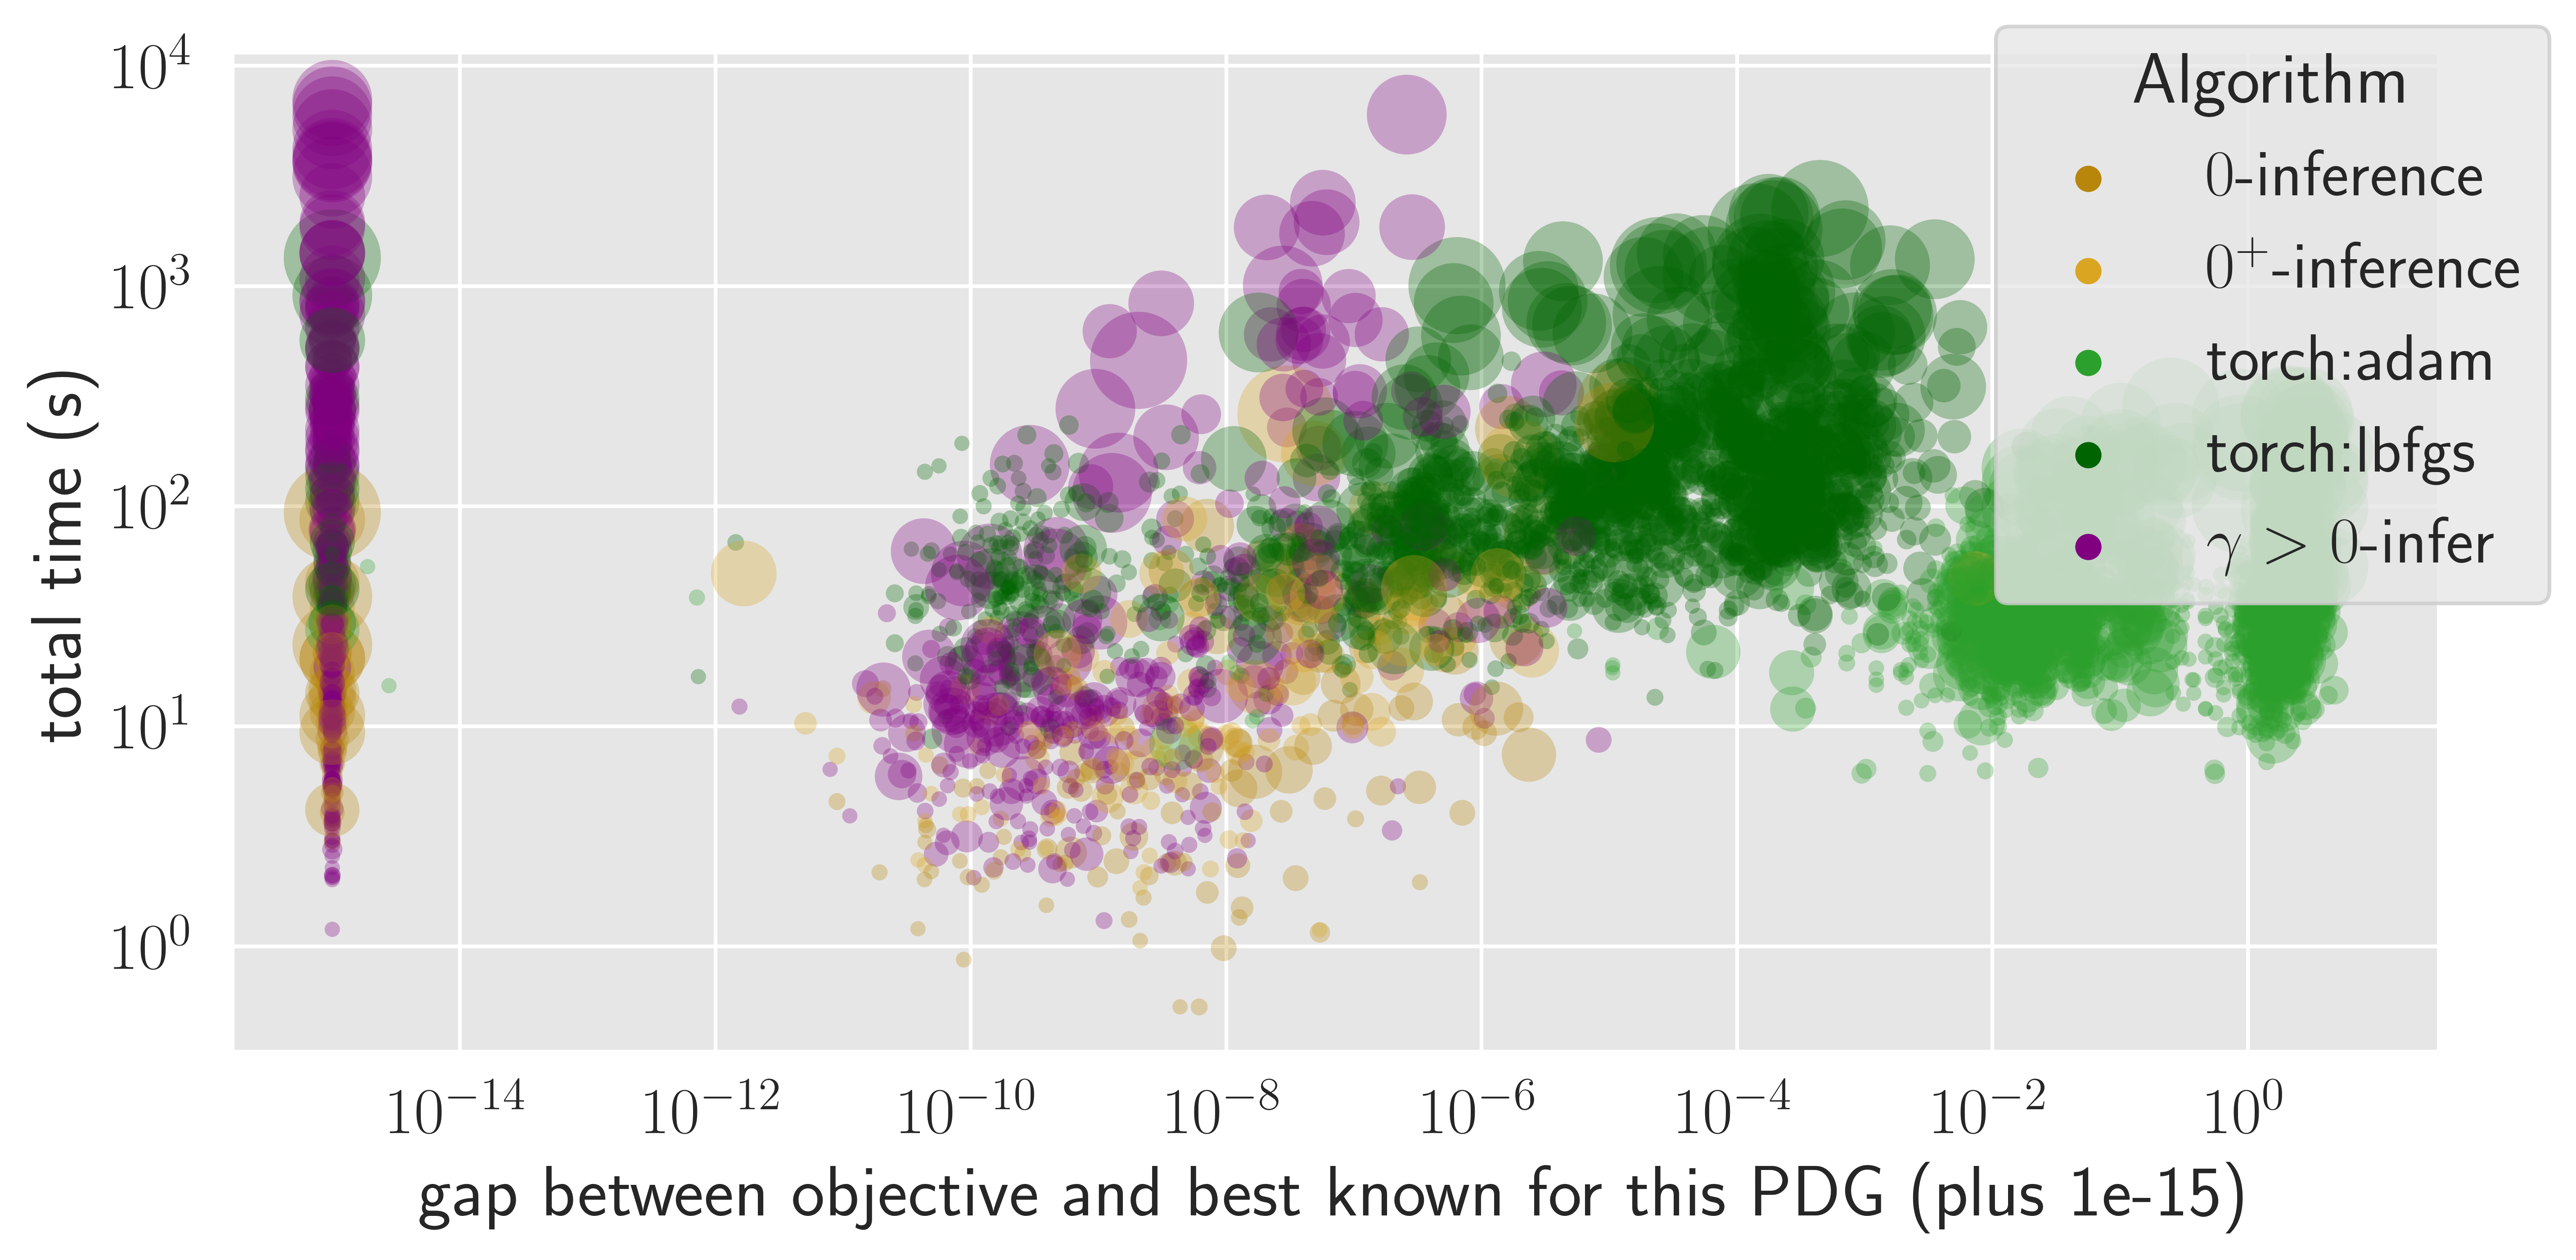
\includegraphics[width=0.67\linewidth]{figs/rand-joint/joint-gap-vs-time-relabeled}
        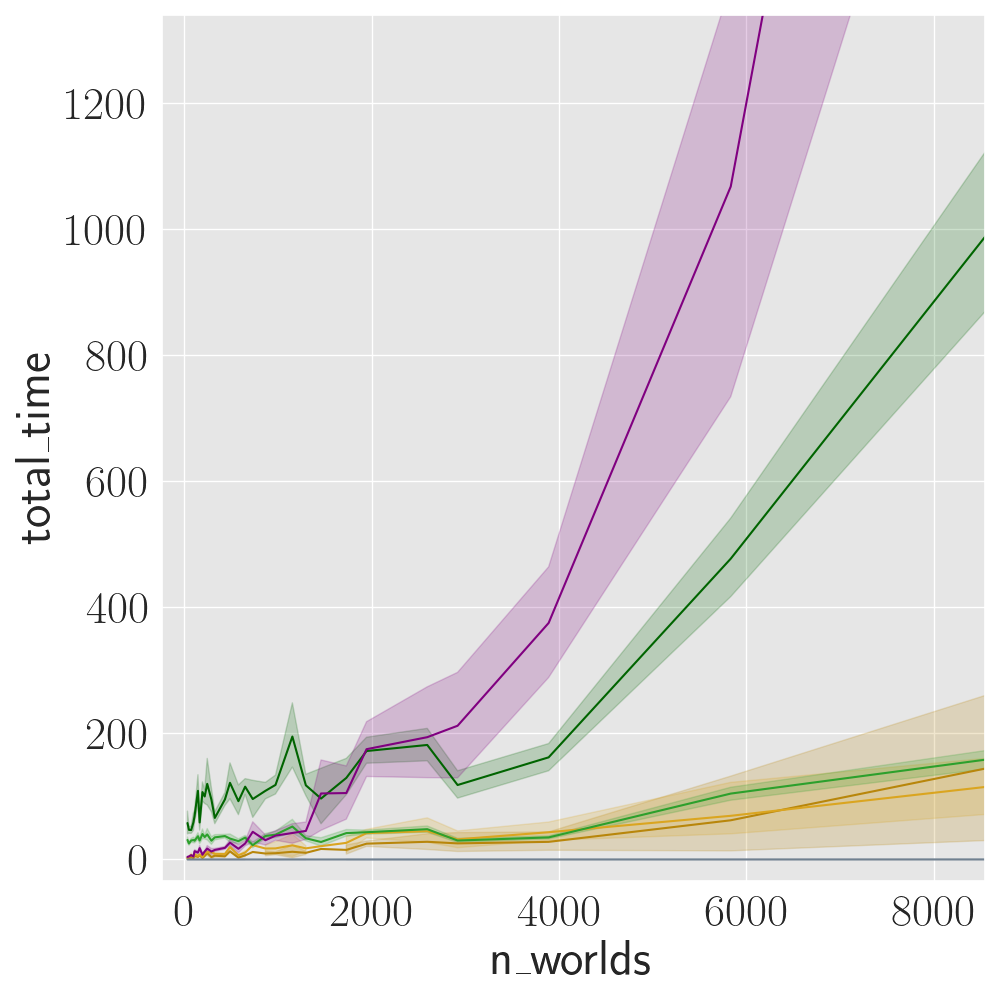
\includegraphics[width=0.32\linewidth]{figs/rand-joint/time-diff}
    \caption[Empirical results: accuracy and resource costs for the inference algorithm and baselines]{
        Accuracy and resource costs for the methods in \cref{sec:inf-as-cvx-program}.  
        Left: a scatter plot of several algorithms on random PDGs of $\approx 10$ variables. The x-axis is 
            the difference in scores
            $\bbr{\dg M}_\gamma(\mu) - \bbr{\dg M}_{\gamma}(\mu^*) + 10^{-15}$,
        where $\mu$ is the method's output,
        and $\mu^*$ achieves best (smallest) known value of $\bbr{\dg M}_{\gamma}$.
         (Thus, the best solutions lie on the far left.)
        The $y$ axis is the time required to compute $\mu$. 
        Our methods are in gold $(0^+$\!-inference) and violet ($\zogamma$-inference, for $\zogamma>0$); the baselines (black-box optimizers applied directly to \eqref{eqn:scoring-fn}) are in green.
        The area of each circle is proportional to the size of the optimization problem, as measured by
        {\small\texttt{n\_worlds}}$:=$
        $|\V\!\X|$.
        Right: how the same methods scale in run time, as $|\V\!\X|$ increases.
     }\label{fig:joint-gap-time}
\end{figure*}

We have given the first algorithm to provably do inference in polynomial
time, but that does not mean that it is the best way of answering queries in practice;
it also makes sense to use black-box optimization tools such as
    Adam \parencite{kingma2014adam} or L-BFGS \parencite{fletcher2013practical}
    to find minimizers of $\bbr{\dg M}_\gamma$.
Indeed, this scoring function has several properties
    that make it highly amenable to such methods: it is
    infinitely differentiable, $\gamma$-strongly convex, and its
    derivatives have simple closed-form expressions.
So it may seem surprising that $\bbr{\dg M}_\gamma$ poses
a challenge to standard optimization tools---%
but it does, 
even when we optimize directly over joint distributions.



\textbf{Synthetic Experiment 1 ({\normalfont over joint distributions}).~~} 
Repeatedly do the following.
First, randomly generate a small PDG $\dg M$ containing 
at most 10 variables and 15 arcs. 
Then for various values of
$\gamma \in \{0, 0^+, 
    10^{-8}, 
     \ldots, \min_a \frac{\beta_a}{\alpha_a} \}$,
optimize $\bbr{\dg M}_\gamma(\mu)$ over joint distributions $\mu$, 
in one of two ways. 
\begin{enumerate}[wide,label=(\alph*),nosep,itemsep=0.2ex]
\item Use \verb|cvxpy| \parencite{diamond2016cvxpy}
to feed  
one of problems (\ref{prob:joint-inc},\ref{prob:joint-small-gamma},\ref{prob:joint+idef})
    to the MOSEK solver \parencite{mosek}, or
\item Choose a learning rate and a representation of $\mu$ in terms of optimization variables $\theta \in \mathbb R^n$.
    Then run a standard optimizer (Adam or L-BFGS) built into \verb|pytorch| \parencite{pytorch}
    to optimize $\theta$
    until $\mu_\theta$ converges to a minimizer of $\bbr{\dg M}_\gamma$ 
        (or a time limit is reached).
    Keep only the best result across all learning rates. 
\end{enumerate}

\begin{figure*}
    \centering
    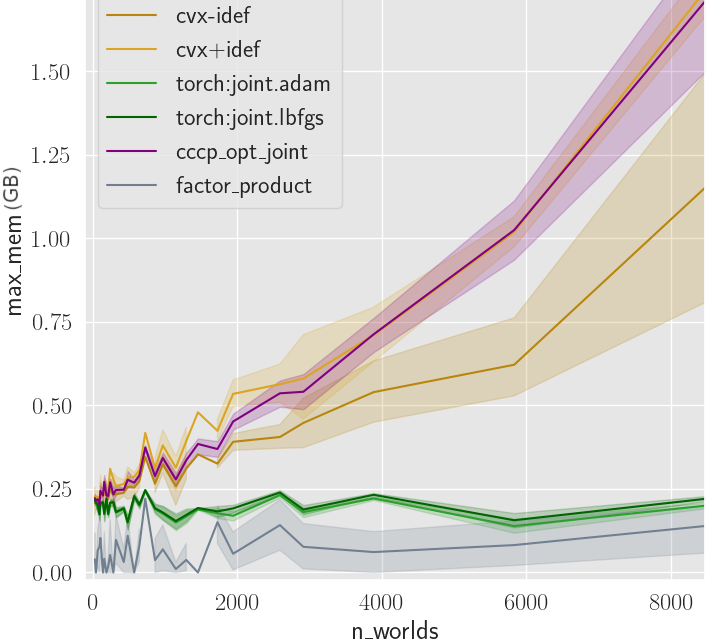
\includegraphics[width=0.34\linewidth]{figs/rand-joint/mem-costs.png}
    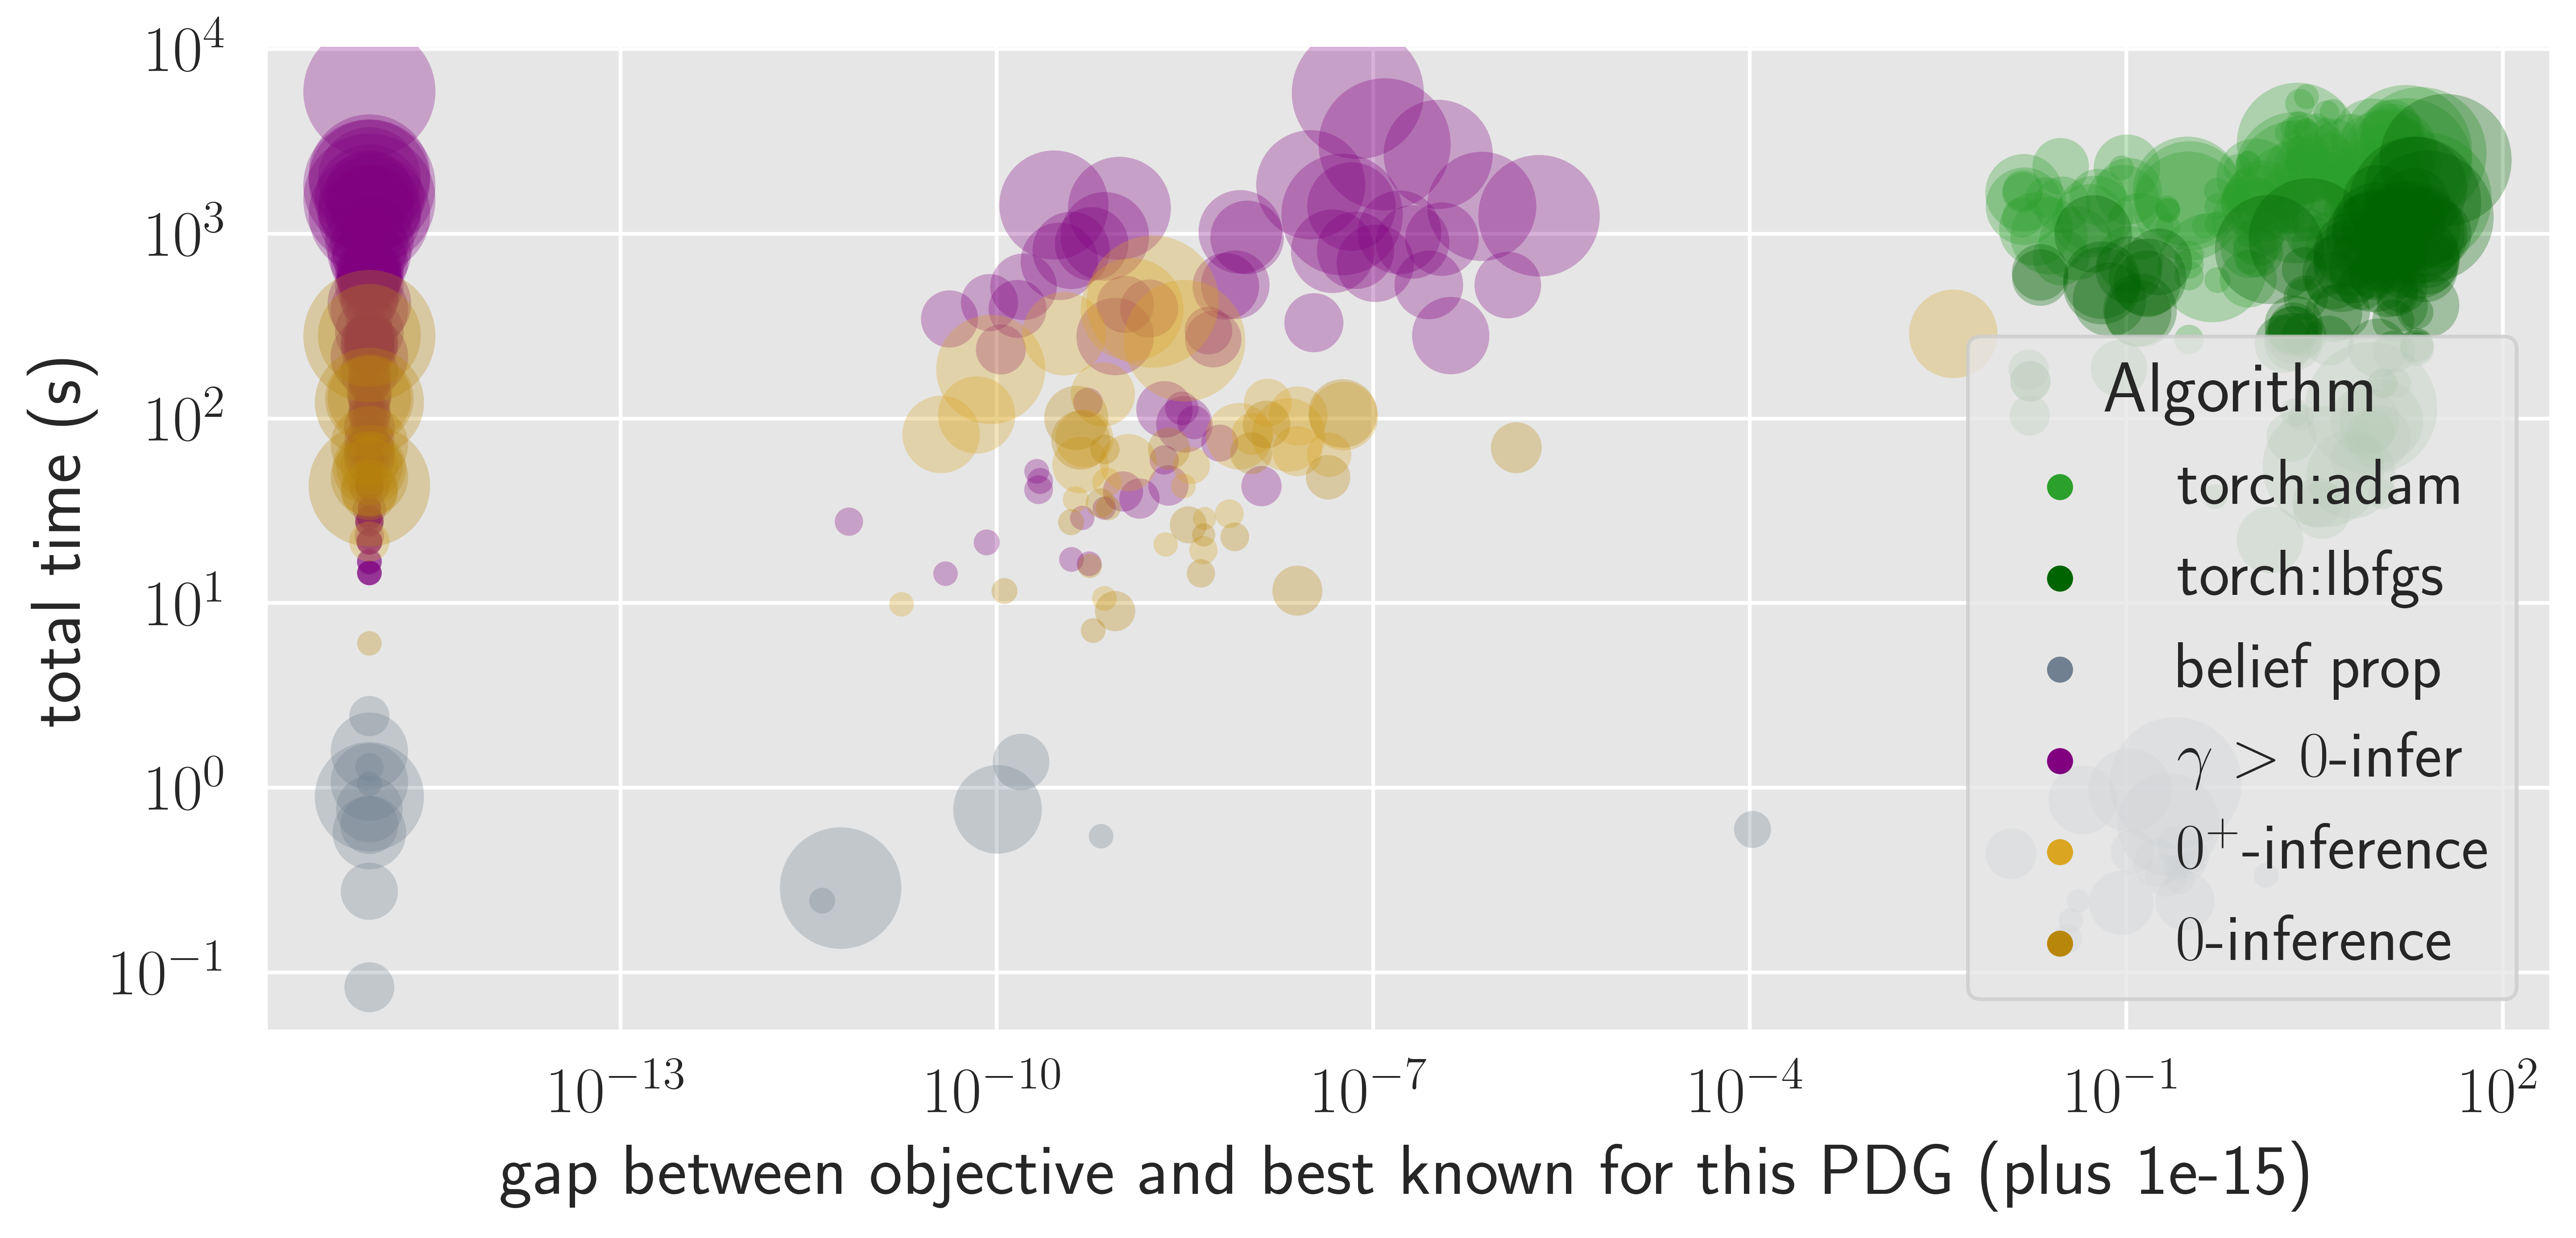
\includegraphics[width=0.65\linewidth]{figs/rand-clus/gap-vs-time-agg9.png}
    \caption[Comparison of convex solver and black-box optimization baselines. Memory footprints, and accuracy/time costs for the cluster setting.]
    {%
    Left: Memory footprint.
    The convex solver (violet, gold)
     requires more memory than baselines (green).
    Right: Analogue of \cref{fig:joint-gap-time} for the cluster setting.
     Here there is even more separation between exponential conic optimization
         (gold, violet) and black-box optimization (greens).
     The grey points represent belief propagation, which is fastest and most accurate---%
         but only applies in the special case when $\bbeta=\gamma\balpha$.}
    \label{fig:joint-mem}
    \label{fig:clus-gap-vs-time}
\end{figure*}


The results are shown in \cref{fig:joint-gap-time}.
Observe that the convex solver (gold, violet) is significantly more accurate than the baselines,
and also much faster for small PDGs.
Our implementation of $0^+\!$-inference (gold) also appears to scale better than L-BFGS
    in this regime, although
    that of $\zogamma$-inference (purple) seems to scale much worse. 
We suspect that the difference comes from \verb|cvxpy|'s compilation process,
    because the two use similar amounts of memory (\cref{fig:joint-mem}),
    and so are problems of similar sizes.



\textbf{Synthetic Experiment 2 ({\normalfont over \actree s}).~~} 
For PDGs of bounded treewidth, \Cref{coro:can-use-cliquetree} allows us to express these optimization problems compactly not just for the convex solver, but for the black-box baseline approaches as well.
We adapt the previous experiment for \actree s as follows.
First randomly sample a maximal graph $G$ of tree-width $k$, called a 
    $k$-tree \parencite{patil1986structure}; 
then generate a PDG $\dg M$ whose hyperarcs lie within cliques of $G$.
This ensures that the maximal cliques of $G$ form a tree-decomposition $(\C, \mathcal T)$ of $\dg M$'s underlying
    hypergraph.
We can now proceed as before: 
    either encode
    (\ref{prob:cluster-inc},\ref{prob:cluster-small-gamma},\ref{prob:cluster+idef})
    as disciplined convex programs in \verb|cvxpy|,
or use \verb|torch| to directly minimize $\bbr{\dg M}_\gamma(\Pr_{\!\bmu})$
    amongst \actree s $\bmu$ over $(\C, \mathcal T)$.
    

In the latter case, however, there is now an additional difficulty:
    it is not easy to strictly enforce the calibration constraints with the black-box methods.
Common practice is to instead add extra loss terms to ``encourage'' calibration---%
but
    it can still be worthwhile for the optimizer to simply incur that loss 
    in order to violate the constraints.
Thus, for fairness, we must recalibrate the 
    the \actree s returned by all methods before evaluation.
The result is an even more significant advantage for the convex solver; 
see \cref{fig:clus-gap-vs-time}.

\textbf{Evaluation on BNs.~~}
We also applied the procedure of the Synthetic Experiment 2
to the smaller BNs in the
\href{https://www.bnlearn.com/bnrepository/}{\texttt{bnlearn}} repository,
and found similar results (but with fewer examples; see \cref{sec:bn-expt-details}). 
But for a PDG that happens to also be a BN, it is possible to use belief propagation, which is much faster and at least as accurate.

Explicit details about all of our experiments, 
and many more figures, can be found in \cref{sec:expt-setup}.

\section{Discussion and Conclusion}

In this chapter, we have provided the first practical algorithm for
    inference in PDGs. 
In more detail, we have defined a parametric family of PDG inference notions, 
given a fixed-parameter tractable inference algorithm for a subset of these parameters,
    proven our algorithm correct, implemented it, and
    shown our code to empirically outperform baselines.
Yet many questions about PDG inference remain open.

Asymptotically, there may be a lot of room for improvement.
Our implementation runs in time $\tilde O(N^4)$, and our analysis suggests one of time $\tilde O(N^{2.872})$. 
But assuming bounded tree-width, most graph problems, including
inference inference for BNs and FGs, can be solved in time $O(N)$. 


Furthermore, we have shown how to do inference for only a subset of
possible parameter values, specifically, 
when
either $\bbeta \ge \gamma \balpha$ or $\bbeta \gg \balpha$. 
The remaining cases are also of interest, and likely require different techniques. 
When $\bbeta = 0$ and $(\Ar, \balpha)$ encodes the structure of a BN,
    for instance,
    inference is about characterizing the BN's independencies.
While we do not know how to tackle 
the inference problem in the general setting, 
our methods can be augmented with the convex-concave procedure 
    \parencite{yuille2003concave} to obtain an inference
    algorithm that applies slightly more broadly; see \cref{sec:cccp}.
We imagine that this extension could also be useful for computing with PDGs 
    beyond the specific inference problem considered in this chapter.

% \vfull{
Our analysis does not resove these problems, but it
    does shed light on some of them.  
The $0$-semantics, for instance, is 
characterized by \cref{prop:marginonly,prop:cluster-inc-correct}, 
Also, when $\bbr{\dg M}_\gamma$ is not convex, we can still find an optimal distribution with the concave-convex procedure \cite{yuille2003concave}, which we do in \cref{sec:cccp}---but this only suffices for inference if we already know there's a unique optimal distribution.
In some cases, this might actually allow us to do inference---say, if we happen to know for external reasons that $\bbr{\dg M}^*_\gamma$ is pseudo-convex (although we loose polynomial time guarantees and have no ability to automatically recognize such situations). In any case, we have implemented this, and describe it in \cref{sec:cccp}.
% }


Given the long history of improvements to our
understanding of inference for 
    Bayesian networks,
we are optimistic that 
    faster and more general
    inference algorithms
    for PDGs
    are possible.



\begin{subappendices}
\relax

\section{Proofs}

Our results fall broadly into three categories:
\begin{enumerate}
    \item Foundational results about PDGs that we needed to prove to get an
        inference procedure, but which are likely to be generally useful
        for anyone working with PDGs
            (\cref{proofs:novel-pdg-results});
    \item Correctness and efficiency results, showing that the optimization
        problems we present in the body of the chapter give the correct answers,
        and that they can be formulated and solved in polynomial time;
            (\cref{proofs:expcone-efficient-correct})
    \item Hardness results, i.e., \cref{theorem:inf-via-inc-oracle} and
    the constructions and lemmas needed to support it
        (\cref{proofs:hardness-results}).
\end{enumerate}

% \subsection{Novel Results about PDGs}
\subsection{Properties of PDG Semantics Needed for Inference}
    \label{proofs:novel-pdg-results}

\recall{prop:marginonly}
\begin{lproof}\label{proof:marginonly}
    For contradiction, suppose that $\mu_1, \mu_2 \in \bbr{\dg M}_0^*$, but
    there is some $(\hat a, \hat s, \hat t) \in \V\!\Ar$ such that $\beta_a > 0$ and
    \[
        \mu_1(\Tgt a{=}\hat t, \Src a{=}\hat s)\mu_2(\Src a{=}\hat s) \ne \mu_2(\Tgt a{=}\hat t, \Src a{=}\hat s) \mu_1(\Src a\hat s).
    \]
    For $t \in [0,1]$,
    let $\mu_t := (1-t) \mu_0 + t \, \mu_1$ as before.
    Then define
    \begin{align*}
        F(t) := \kldiv[\Big]{ \mu_t(\Src a, \Tgt a) }{  \mu_t(\Src a) \p_a(\Tgt a|\Src a) }.
    \end{align*}
    Since $\mu_0(\Src a, \Tgt a)$ and  $\mu_1(\Src a, \Tgt a)$ are joint distributions over two variables, with different conditional marginals, as above, \cref{lem:seg-strictcvx} applies, and so $F(t)$ is strictly convex.

    Let
    \[ \OInc_{\dg M \setminus \hat a}
        := \sum_{a \ne \hat a} \beta_a \kldiv{\mu(\Tgt a, \Src a)}{\p_a(\Tgt a|\Src a) \mu(\Src a)}
    \]
    be the observational incompatibility loss, but without the term corresponding to edge $\hat a$.
    Since $\OInc_{\dg M \setminus \hat a}$ is convex in its argument, it is in particular convex along the segment from $\mu_0$ to $\mu_1$; that is, for $t \in [0,1]$, the function $t \mapsto \OInc_{\dg M \setminus \hat a}(\mu_t)$ is convex.
    Therefore, we know that the function
    \begin{align*}
        G(t) :=
        \OInc_{\dg M}(\mu_t)
        =
        \OInc_{\dg M \setminus a}( \mu_t ) + \beta_a\, F(t),
    \end{align*}
    is \emph{strictly} convex.
    But then this means $\mu_{\nf12}$ satisfies
    \[
        \OInc_{\dg M}( \mu_{\nicefrac12} ) < \OInc_{\dg M}( \mu_0 ),
    \]
    contradicting the premise that $\mu_0$ minimizes $\OInc_{\dg M}$ (i.e., $\mu_0 \in \bbr{\dg M}^*_0$).
    Therefore, it must be the case that all distributions in $\bbr{\dg M}_0^*$ have the same conditional marginals, as promised.
\end{lproof}

\clearpage
\recall{prop:idef-frozen}
\begin{lproof}\label{proof:idef-frozen}
    This is mostly a simple algebraic manipulation. By definition:
    \begin{align*}
        \SDef_{\dg M}(\mu) &= - \H(\mu) + \sum_{a \in \Ar} \alpha_a \H_\mu(\Tgt a | \Src a) \\
        &= \Ex_\mu \left[ - \log \frac{1}{\mu} + \sum_{a \in \Ar} \alpha_a \log \frac{1}{\mu(\Tgt a|\Src a)} \right] \\
        &= \sum_{w \in \V\!\X} \mu(w) \left[ \log \mu(w) + \sum_{a \in \Ar} \log \frac{1}{\mu(\Tgt a(w)|\Src a(w))^{\alpha_a}} \right] \\
        &= \sum_{w \in \V\!\X} \mu(w) \log \pqty[\bigg]{ \faktor{\mu(w)~}{~\prod_{a \in \Ar}\mu(\Tgt a(w)|\Src a(w))^{\alpha_a}}}
    \end{align*}
    But, by \cref{prop:marginonly}, if we restrict $\mu \in \bbr{\dg M}_0^*$, then the conditional marginals in the denominator do not depend on the particular choice of $\mu$; they're shared among all $\nu \in \bbr{\dg M}_0^*$.
\end{lproof}


\recall{theorem:markov-property}

\[
    \text{Or symbolically: }\qquad\quad
    \dg M_1 \bundle \dg M_2
        ~\models~
    \X_1 \mathbin{\bot\!\!\!\bot} \X_2 \mid \X_1 \cap \X_2. \]
\begin{lproof}\label{proof:markov-property}
    Note that,
    save for the joint entropy, every summand the scoring function $\bbr{\dg M_1 + \dg M_2}_\gamma : \Delta(\V\!\X_1 \times \V\!\X_2)$, is a function of the conditional marginal of $\mu$ along some edge.
    In particular, those terms that correspond to edges of $\dg M_1$ can be computed from the marginal $\mu(\X_1)$, while those that correspond to edges of $\dg M_2$ can be computed from the marginal $\mu(\X_2)$.
    Therefore, there are functions $f$ and $g$ such that:
    \[
        \bbr{\dg M_1 \bundle \dg M_2}_\gamma(\mu) = f(\mu(\X_1)) + g(\mu(\X_2)) - \gamma \H(\mu).
    \]

    To make this next step extra clear, let $\mat X := \X_1 \setminus \X_2$ and
    $\mat Z := \X_2 \setminus \X_1$, be the variables unique to each PDG, and $\mat S:= \X_1 \cap \X_2$ be the set of variables they have in common, so that $(\mat X, \mat S, \mat Z)$ is a partition of all variables $\mat X_1 \cup \mat X_2$.
    Now define a new distribution $\mu' \in \Delta(\V\!\X_1 \times \V\!\X_2)$ by
    \[
        \bf
        \mu'( X,  S,  Z)
            := \mu(S) \mu( Z \mid  S)\mu( X \mid  S)
            \qquad \Big(~
            = \mu( X,  S) \mu( Z \mid  S)
            = \mu( Z,  S) \mu( X \mid  S)~\Big).
    \]
    One can easily verify that $\mat X$ and $\mat Z$ are independent given $\mat S$ in $\mu'$ (by construction), and the alternate forms on the right make it easy to see that $\mu(\X_1) = \mu'(\X_1)$ and $\mu(\X_2) = \mu'(\X_2)$.
    Furthermore, for any $\nu'(\mat{X,S,Z})$, we can write
    \begin{align*}
        \H( \nu ) &=  \H_\nu(\mat{X,S,Z}) =
            \H_\nu(\mat{X,S}) + \H_\nu(\mat Z \mid \mat{X,S}) \\
            &= \H_\nu(\mat{X,S}) + \H_\nu(\mat Z \mid \mat{X,S}) - \H_\nu(\mat Z \mid \mat S) + \H_\nu(\mat Z \mid \mat S) \\
            &= \H_\nu(\mat X,\mat S) + \H_\nu(\mat Z \mid \mat S) - \I_\nu(\mat Z; \mat X| \mat S),
    \end{align*}
    where $\I_\nu(\bf X;Z|S)$, the conditional mutual information between $\mat X$ and $\mat Z$ given $\mat S$ (in $\nu$), is non-negative, and equal to zero if and only if $\mat X$ and $\mat Z$ are conditionally independent given $\mat S$ \parencite[see, for instance,][\S1]{mackay2003information}.
    So $\I_{\mu'}(\mat X; \mat Z| \mat S) = 0$, and
        $\H_{\mu'} = \H_{\mu'}(\mat X, \mat S) + \H_{\mu'}(\mat Z| \mat S)$.
    Because $\mu$ and $\mu'$ share marginals on $\X_1$ and $\X_2$, while the terms $\H(\mat X, \mat S)$ and $\H(\mat Z|\mat S)$ depend only on these marginals, respectively, we also know that $\H_{\mu}(\mat X, \mat S) = \H_{\mu'}(\mat X, \mat S)$ and $\H_{\mu}(\mat Z | \mat S) = \H_{\mu'}(\mat Z| \mat S)$; thus we have
    \begin{align*}
        \H(\mu) &= \H_\mu(\mat X,\mat S) + \H_\mu(\mat Z \mid \mat S) - \I_\mu(\mat Z; \mat X| \mat S) \\
            &= \H(\mu') - \I_\mu(\mat Z; \mat X| \mat S).
    \end{align*}
    Therefore,
    \begin{align*}
        \bbr{\dg M_1 \bundle \dg M_2}_\gamma(\mu)
         &= f(\mu(\X_1)) + g(\mu(\X_2)) - \gamma \H(\mu) \\
         &= f(\mu'(\X_1)) + g(\mu'(\X_2)) - \gamma \H(\mu') + \gamma \I_\mu(\mat Z; \mat X| \mat S) \\
         &= \bbr{\dg M_1 \bundle \dg M_2}_\gamma(\mu') + \gamma \I_\mu(\mat Z; \mat X| \mat S).
    \end{align*}
    But conditional mutual information is non-negative, and by assumption, $\bbr{\dg M \bundle \dg M_2}_\gamma(\mu)$ is minimal. Therefore, it must be the case that
    \[
        \I_\mu(\mat Z; \mat X| \mat S) = \I_\mu(\X_1; \X_2 \mid \X_1 \cap \X_2) = 0,
    \]
    showing that $\X_1$ and $\X_2$ are conditionally independent given the variables that they have in common. \\
    (The fact that $\I_\mu(\mat Z; \mat X| \mat S) = \I_\mu(\X_1; \X_2 \mid \X_1 \cap \X_2)$ is both easy to show and an instance of a well-known identity; see CIRV2 in Theorem 4.4.4 of \textcite{halpern-RAU}, for instance.)
\end{lproof}

\recall{coro:can-use-cliquetree}
\begin{lproof}\label{proof:can-use-cliquetree}

    The set of distributions that can be represented by a \cactree\ over $(\C,\cal T)$ is the same as the set of distributions that can represented by a factor graph for which $(\C, \cal T)$ is a tree decomposition.
    One direction holds because any such product of factors ``calibrated'', via message passing algorithms such as belief propagation, to form a \actree.
    The other direction holds because $\Pr_{\bmu}$ itself is a product of factors that decomposes over $(\C, \cal T)$.



    Alternatively, this same set of distributions that satisfy the independencies of the Markov Network obtained by connecting every pair of variables that share a cluster.
    More formally, this network is the graph $G := (\X, E := \{ (X{-}Y) :  \exists C \in \C.~\{X,Y\} \subseteq C\})$.
    Also, $G$ happens to chordal as well, which we prove at the end.


    Using only the PDG Markov property (\cref{theorem:markov-property}), we now show that every independence described by $G$ also holds in every distribution $\mu \in \bbr{\dg M}^*_\gamma$.
    Suppose that,
    for sets of variables $\mat X, \mat Y, \mat Z \subseteq \X$,
    $\I(\mat X; \mat Y|\mat Z)$ is an independence
    described by $G$.
    This means \parencite[Defn 4.8]{KF09} that
    if $X \in \mat X$, $Y \in \mat Y$, and $\pi$ is a path in $G$ between them, then
    some node along $\pi$ lies in $\mat Z$.


    Let $\cal T'$ be the graph that results from removing each edge $(C{-}D) \in \cal T$ that satisfies $C \cap D \subseteq \mat Z$, which is a disjoint union  $\mathcal T' = \mathcal T_1 \sqcup \ldots \sqcup \mathcal T_n$ of subtrees that have no clusters in common.
    To parallel this notation, let $\C_1, \ldots, \C_n$ be their respective vertex sets.
    Note that for every edge $e=(C{-}D)\in \cal T'$, there must by definition be some variable $U_e \in (C \cap D) \setminus \mat Z$.

    We claim that no subtree $\mathcal T_i$ can have both a cluster $D_X$ containing a variable $X \in \mat X \setminus \mat Z$ and also a cluster $D_Y$ containing a variable $Y \in \mat Y \setminus \mat Z$.
    Suppose that it did.
    Then the (unique) path in $\cal T$ between $D_X$ and $D_Y$, which we label
    \[
    \begin{tikzcd}[column sep=2em]
        D_X=
        &D_0 \ar[r,-,"e_1"]&
        D_1 \ar[r,-,"e_2"]&
          \cdots
        \ar[r,-,"e_{m-1}"]& D_{m-1}
        \ar[r,-,"e_m"] & D_m&
        =D_Y
    \end{tikzcd},
    \]
    would lie entirely within $\mathcal T_i \subseteq \mathcal T'$. This gives rise to
    a corresponding path in $G$:
    \[\begin{tikzcd}[column sep=1em,row sep=1.5ex]
        X \ar[r,-] \ar[d,sloped,phantom,"\in"]
        & U_{e_1}\ar[r,-] \ar[d,sloped,phantom,"\in"]
        & U_{e_2}\ar[r,-] \ar[d,sloped,phantom,"\in"]
           &\cdots\ar[r,-]
        & U_{e_{n{-}1}} \ar[r,-] \ar[d,sloped,phantom,"\in"]
        & U_{e_n}\ar[r,-] \ar[d,sloped,phantom,"\in"]
        & Y \ar[d,sloped,phantom,"\in"]
            \\
        D_0
        & D_0 \cap D_1
        & D_1 \cap D_2
        &
        & D_{n{-}2} \cap D_{n{-}1}
        & D_{n{-}1} \cap D_n
        & D_n
    \end{tikzcd}\quad,\]
    and moreover, this path is disjoint from $\mat Z$.
    This contradicts our assumption that every path in $G$ between a member of $\mat X$ and a member of $\mat Y$ must intersect with $\mat Z$, and so no subtree can have both a cluster containing a variable $X \in \mat X \setminus \mat Z$ and also one containing $Y \in \mat Y \setminus \mat Z$.

    \def\CX{\C_{\mat X}}
    \def\CNX{\C_{\mat{Y}}^+}
    We can now partition the clusters as $\C = \CX \sqcup \CNX$, where
    $\CX$ is the set of the clusters that belong to subtrees $\mathcal T_i$ with a cluster containing some $X \in \mat X \setminus \mat Z$, and
    its $\CNX$ is its complement, which in particular contains those subtrees have some $Y \in \mat Y \setminus \mat Z$.
    Or, more formally, we define
    \[
        \CX :=~ \bigcup_{\mathclap{\substack{i \in \{1,\ldots,n\}\\ (\cup\C_i) \cap (\mat X\setminus\mat Z) \ne \emptyset }}}\, \C_i
        \quad\qquad \text{and}\qquad
        \CNX :=~ \bigcup_{\mathclap{\substack{i \in \{1,\ldots,n\}\\ (\cup\C_i) \cap (\mat X\setminus\mat Z) = \emptyset }}}\, \C_i
        \quad.
    \]
    \def\XX{\X_{\mat X}}
    \def\XNX{\X_{\mat Y}^+}
    Let $\XX := \cup \CX$ set of all variables appearing in the clusters $\CX$; symmetrically, define $\XNX := \cup \CNX$.


    We claim that $\XX \cap \XNX \subset \mat Z$.
    Choose any variable $U \in \XX \cap \XNX$.
    From the definitions of $\XX$ and $\XNX$, this means $U$ is a member of some cluster $C \in \CX$, and also a member of a cluster $D \in \CNX$.
    Recall that the clusters of each disjoint subtree $\mathcal T_i$ either fall entirely within $\CX$ or entirely within $\CNX$ by construction.
    This means that $C$ and $D$, which are on opposite sides of the partition, must have come from distinct subtrees.
    So, some edge $e = (C'{-}D') \in \mathcal T$ along the (unique) path from $C$ to $D$ must have been removed when forming $\mathcal T'$, which by the definition of $\mathcal T'$, means that $(C' \cap D') \subset Z$.
    But by the running intersection property (\actree\ property 2), every cluster along the path from $C$ to $D$ must contain $C \cap D$---in particular, this must be true of both $C'$ and $D'$.
    Therefore,
    \[
        U \in C \cap D \subset C' \cap D' \subset \mat Z.
    \]
    So $\XX \cap \XNX \subset \mat Z$, as promised.  We will rather use it in the equivalent form $(\XX \cap \XNX) \cup \mat Z = \mat Z$.

    Next, since $(\C, \cal T)$ is a tree decomposition of $\Ar$, each hyperarc $a \in \Ar$ can be assigned to some cluster $C_a$ that contains all of its variables; this allows us to lift the cluster partition $\C = \CX \sqcup \CNX$ to a partition $\Ar = \Ar_{\mat X} \sqcup \Ar_{\mat Y}^+$ of edges, and consequently, a partition of PDGs $\dg M = \dg M_{\mat X} \bundle \dg M_{\mat Y}^+$.
    Concretely: let $\dg M_{\mat X}$ be the sub-PDG of $\dg M$ induced by restricting to the variables $\XX \subseteq \X$ arcs $\Ar_{\mat X} = \{ a \in \Ar : C_a \in \CX \} \subseteq \Ar$; define $\dg M_{\mat Y}^+$ symmetrically. (To be explicit: the other data of $\dg M_{\mat X}$ and $\dg M_{\mat Y}^+$ are given by restricting each of $\{\mathbb P,\balpha,\bbeta\}$ to $\Ar_{\mat X}$ and $\Ar_{\mat Y}^+$, respectively.)

    This partition of $\dg M$ allows us to use the PDG Markov property.
    Suppose that for some $\gamma > 0$ that $\mu \in \bbr{\dg M}^*_\gamma = \bbr{\dg M_{\mat X} \bundle \dg M_2}^*_\gamma$.
    We can then apply \cref{theorem:markov-property}, to find that
    $\XX$ and $\XNX$ are independent given $\XX \cap \XNX$.
    We use standard standard properties of random variable independence
        \parencite[CIRV1-5 of][Theorem 4.4.4]{halpern-RAU} to find that $\mu$ must satisfy:
    \begin{align*}
        \XX  &\CI \XNX \mid \XX \cap \XNX\\
    \implies~~~
        (\XX \setminus \mat Z) &\CI (\XNX\setminus \mat Z) \mid (\XX \cap \XNX) \cup \mat Z
            & \big[\,\text{CIRV3}\,\big] \\
    \implies\quad
        (\mat X \setminus \mat Z) &\CI (\mat Y \setminus \mat Z) \mid (\XX \cap \XNX) \cup \mat Z
        % & \big[\,\text{by CIRV2, as $\mat X \subseteq \XX$ and $\mat Y \subseteq \XNX$}\,\big] \\
        & \Big[\singlespacing\begin{array}{l}\text{by CIRV2, as }\\\mat X \subseteq \XX\text{ and }\mat Y \subseteq \XNX \end{array}\big] \\
    \implies\quad
        (\mat X \setminus \mat Z) &\CI (\mat Y \setminus \mat Z) \mid \mat Z
        & \big[\,\text{since $(\XX \cap \XNX) \cup \mat Z = \mat Z$}\,\Big] \\
    \iff\quad
        \mat X &\CI \mat Y \mid \mat Z
        & \hspace{-6em}\big[\,\text{standard; e.g., Exercise 4.18 of \textcite{halpern-RAU}}\,\big] \\
    \end{align*}

    Using only the PDG Markov property, we have now shown that every independence
    modeled by the Markov Network $G$ also holds
    in every distribution $\mu \in \bbr{\dg M}^*_\gamma$. Moreover, $G$ is chordal (as we will prove momentarily),
    and is well-known that distributions that have the independencies of a chordal graph can be can be represented by \actree s \parencite[Theorem 4.12]{KF09}.
    Therefore, there is a \actree $\bmu$ representing every $\mu \in \bbr{\dg M}^*_\gamma$.

    \begin{iclaim}
        $G$ is chordal.
            \label{subclaim:chordal}
    \end{iclaim}
    \begin{proof}
        Suppose that $G$ contains a loop $X{-}Y{-}Z{-}W{-}X$.
        Suppose further, for contradiction, that neither $X$ and $Z$ nor $Y$ and $W$ share a cluster.
        Given a variable $V$, it is easy to see that property (2) of the tree decomposition ensures that the subtree $\mathcal T(V) \subseteq \mathcal T$ induced by the clusters $C \in \C$ that contain $V$, is connected.
        By assumption, ${\cal T}(Y)$ and ${\cal T}(W)$ must be disjoint.
        There is an edge between $Y$ and $Z$, so some cluster must contain both variables, meaning ${\cal T}(Y) \cap {\cal T}(Z)$ is non-empty.
        Similarly, ${\cal T}(Z) \cap {\cal T}(W)$ is non-empty because of the edge between $Z$ and $W$.
        This creates an (indirect) connection in $\cal T$ between ${\cal T}(Y)$ and ${\cal T}(W)$. Because $\cal T$ is a tree, and ${\cal T}(Y) \cap {\cal T}(W) = \emptyset$,
        every path from a cluster $C_1 \in {\cal T}(Y)$ to a cluster $C_2 \in {\cal T}(W)$ must pass through ${\cal T}(Z)$, which is not part of ${\cal T}(Y)$ or ${\cal T}(W)$.
        ${\cal T}(X)$ and ${\cal T}(Y)$ intersect as well, meaning that, for any $C \in {\cal T}(X)$, there is a (unique) path from $C$ to that point of intersection, then across edges of ${\cal T}(Y)$, then edges of ${\cal T}(Z)$, and finally connects to the clusters of ${\cal T}(W)$. And also, since $\cal T$ is a tree, that path must be unique.
        The problem is that there is also an edge between $X$ and $W$, so there's some cluster that contains $X$ and $W$; let's call it $C_0$.
        It's distinct from the cluster $D_0$ that contains $Z$ and $W$, since no cluster contains both $X$ and $Z$ by assumption.
        The unique path from $C_0$ to $D_0$
        intersects with ${\cal T}(Y)$.
        But now $W \in C_0 \cap D_0$, and by the running intersection property, every node along this unique path must contain $W$ as well.
        But this contradicts our assumption that $W$ is disjoint from $Y$! So $G$ is chordal.
    \end{proof}
    Having proved the subclaim \cref{subclaim:chordal}, 
    we have now finished the proof of \cref{coro:can-use-cliquetree}.
\end{lproof}


% \subsection{Correctness and Efficiency of Inference via Exponential Conic Programming}
\subsection{Correctness and Complexity Analysis for PDG Inference via Exponential Conic Programming}
    \label{proofs:expcone-efficient-correct}

\recall{prop:joint-inc-correct}

\begin{lproof}
    \label{proof:joint-inc-correct}
    Suppose that $(\mu, \mat u)$ is a solution to \eqref{prob:joint-inc}.
    The exponential cone constraints ensure that, for every $(a, s,t) \in \V\!\Ar$,
    \[
        u_{a,s,t} \ge \mu(s,t) \log \frac{\mu(s,t)}{\p_a(t|s)\mu(s)},
    \]
    where $\mu(s,t)$ and $\mu(s)$, as usual, are shorthand for $\mu(\Src a{=}s, \Tgt a{=}t)$ and $\mu(\Src a {=} s)$, respectively.
    %
    Suppose, for contradiction, that one of these inequalities is strict at some an index $(a',s',t') \in \V\!\Ar$ for which $\beta_{a'} > 0$.
    Explicitly, this means
    \[
        u_{a',s',t'} > \mu(s_0,t_0) \log \frac{\mu(s',t')}{\p_{a'}(t'|s')\mu(s')}.
    \]
    In that case, we can define a vector $\mat u' = [u'_{a,s,t}]_{(a,s,t)\in\V\!\Ar}$ which is identical to $\mat u$, except that at $(a',s',t')$, it is halfway between the two quantities described as different above.  More precisely:
    \[
        u'_{a',s',t'} = \frac12 u_{a',s',t'} + \frac12 \log \mu(s',t') \log \frac{\mu(s',t')}{\p_a(t'|s')\mu(s')}.
    \]
    Note that $u'_{a',s',t'} < u_{a',s',t'}$,
    and also that, by construction, $(\mu, \mat u')$ also satisfies the constraints of \eqref{prob:joint-inc}.
    In more detail: at the index $(a', s', t')$,
    $\mat u'$ does not violate the associated exponential cone constraint
    $$
        \left( \text{because}~ 
        u'_{a',s',t'} = \frac12 u_{a',s',t'} + \frac12 \log \mu(s',t')\log \frac{\mu(s',t')}{\p_{a'}(t'|s')\mu(s')}
        >
        \mu(s',t') \log \frac{\mu(s',t')}{\p_{a'}(t'|s')\mu(s')}
        \right),
    $$
    and $\mat u'$ equals $\mat u$ at other indices, and therefore satisfies the constraint everywhere else as well.
    But now, because $u'_{a', s', t'} < u_{a',s',t'}$, and $\beta_{a'} >0$, we also have
    \[
        \sum_{(a,s,t) \in \V\!\Ar} \beta_a u'_{a,s,t}
            > \sum_{(a,s,t) \in \V\!\Ar} \beta_a u'_{a,s,t}.
    \]
    Thus the objective value at $(\mu, \mat u')$ is strictly
    smaller than the one at $(\mu, \mat u)$, both of which are feasible points.
    This contradicts the assumption that $(\mu, \mat u)$ is optimal.
    We therefore conclude that none of these inequalities can be strict at points where $\beta_{a} > 0$.
    This can be compactly written as:
    \begin{align*}
        \forall (a,s,t) \in \V\!\Ar.\quad
        \beta_a u_{a,s,t} &= \beta_a \mu(s,t) \log \frac{\mu(s,t)}{\p_a(t|s)\mu(s)} \\
        \implies\qquad
        \sum_{(a,s,t) \in \V\!\Ar}\beta_a u_{a,s,t}
            &= \sum_{(a,s,t) \in \V\!\Ar} \beta_a \mu(s,t) \log \frac{\mu(s,t)}{\p_a(t|s)\mu(s)}
            = \OInc_{\dg M}(\mu).
    \end{align*}
    In other words, the objective of problem \eqref{prob:joint-inc} at
    $(\mu, \mat u)$ is equal to the observational incompatibility $\OInc_{\dg M}(\mu)$ of $\mu$ with $\dg M$.
    And, because $(\mu, \mat u)$ minimizes this value among all joint distributions, $\mu$ must be a minimum of $\OInc_{\dg M}$.

    More formally: assume for contradiction that $\mu$ is not a minimizer of $\OInc_{\dg M}$. Then there would be some other distribution $\mu'$ for which $\OInc_{\dg M}(\mu') < \OInc_{\dg M}(\mu)$.
    Let $\mat u'' := [ \mu'(s,t) \log \frac{\mu'(s,t)}{\p_a(t|s) \mu'(s)} ]_{(a,s,t) \in \V\!\Ar}$. Clearly $(\mu', \mat u'')$ satisfies the constraints of the problem, and moreover,
    \[
        \sum_{(a,s,t)\in \V\!\Ar} \beta_a u_{a,s,t} =
        \OInc_{\dg M}(\mu) >
        \OInc_{\dg M}(\mu') =
        \sum_{(a,s,t)\in \V\!\Ar} \beta_a u'_{a,s,t},
    \]
    contradicting the assumption that the $(\mu, \mat u)$ is optimal for problem \eqref{prob:joint-inc}. Thus, $\mu$ is a minimizer of $\OInc_{\dg M}$, and the objective value is $\inf_{\mu} \OInc_{\dg M}(\mu) = \aar{\dg M}_0$, as desired.
\end{lproof}

\recall{prop:joint-small-gamma-correct}
For convenience, we repeat problem \eqref{prob:joint-small-gamma}
(left) and an equivalent variant of it that we implement (right) below.
\begin{center}
\footnotesize	
\makebox[0pt]{%
\begin{minipage}{0.52\linewidth}
\begin{align*}
\minimize_{\mu, \mat u, \mat v} & ~~
    \sum_{\mathrlap{\!\!\!(a,s,t) \in \V\!\Ar}}
        (\beta_a \!- \alpha_a \gamma) u_{a,s,t}
        \,+
        \gamma
        \sum_{\mathclap{w \in \V\!\X}} v_w
    \tag{\ref{prob:joint-small-gamma}}
\\[-0.2ex]
    &
    - \sum_{\mathrlap{\!\!\!(a,s,t) \in \smash{\V\!\Ar^+}}}
        \alpha_a \gamma \,
        \mu(\Src a{=}s,\Tgt a {=} t) \log \p_a (t|s)
\\[0.2ex]
\subjto&\quad \mu \in \Delta\V\!\X,
        \quad ( -\mat v,  \mu,  \mat 1) \in K_{\exp}^{\V\!\X},
\\[-0.4ex]
    \forall a \in \Ar.~
        &\big(\shortminus\mat u_a, \mu( \Tgt a,\Src a),\p_a(\Tgt a | \Src a)  \mu(\Src a) \big)
            \in K_{\exp}^{\V a},
\\[-0.2ex]
    \forall (a,s,t) &\in \V\!\Ar^0\!.~
    \mu(\Src a{=}\mskip2mus, \Tgt a{=}\mskip2mut) = 0;
\end{align*}
\end{minipage}
~~\vrule~~
\begin{minipage}{0.52\linewidth}
\begin{align*}
\minimize_{\mu, \mat u, \mat v} & ~~
    \sum_{\mathrlap{\!\!\!(a,s,t) \in \V\!\Ar}}
        (\beta_a \!- \alpha_a \gamma) u_{a,s,t}
        \,+
        \gamma
        \sum_{\mathclap{w \in \V\!\X}} v_w
        \tag{\ref*{prob:joint-small-gamma}b}\label{prob:joint-small-gamma-b}
\\[-0.2ex]
    &
    - \sum_{\mathrlap{\!\!\!(a,s,t) \in \smash{\V\!\Ar^+}}}
        \beta_a \,
        \mu(\Src a{=}s,\Tgt a {=} t) \log \p_a (t|s)
\\[0.2ex]
\subjto&\quad \mu \in \Delta\V\!\X,
        \quad ( -\mat v,  \mu,  \mat 1) \in K_{\exp}^{\V\!\X},
\\[-0.4ex]
    \forall a \in \Ar.~
    &\big(\shortminus\mat u_a, \mu( \Tgt a,\Src a),
        \big[\,\mu(\Src a{=}s) \big]_{(s,t) \in \V a} \big)
        \in K_{\exp}^{\V a},
\\[-0.2ex]
    \forall (a,s,t) &\in \V\!\Ar^0\!.~
    \mu(\Src a{=}\mskip2mus, \Tgt a{=}\mskip2mut) = 0.
\end{align*}
\end{minipage}
}
\end{center}
\medskip

\begin{lproof}\label{proof:joint-small-gamma-correct}
    We start with the problem on the left, which is \eqref{prob:joint-small-gamma} from the main text.
    Suppose that $(\mu, \mat u, \mat v)$ is a solution to \eqref{prob:joint-small-gamma}.
    The exponential constraints ensure that
    \[
        \forall (a,s,t) \in \V\!\Ar.~
        u_{a,s,t} \ge \mu(s,t) \log \frac{\mu(t|s)}{\p_a(t|s)}
    \qquad\text{and}\qquad
        \forall w \in \V\!\X.~
        v_{w} \ge \mu(w) \log \mu(w).
    \]
    As in the previous proof, we claim that these must hold with equality (except possibly for $u_{a,s,t}$ at indices satisfying $\beta_a = \gamma \alpha_a$, when it doesn't matter).
    This is because otherwise one could reduce the value of a component of $u$ or $v$ while still satisfying all of the constraints, to obtain a strictly smaller objective, contradicting the assumption that $(\mu, \mat u, \mat v)$ minimizes it.

    Thus, $\mat v$ is a function of $\mu$, as is every value of $\mat u$ that affects the objective value of \eqref{prob:joint-small-gamma}, meaning that this objective value can be written as a function of $\mu$ alone:
    \begin{align*}
        &\sum_{\mathrlap{\!\!\!(a,s,t) \in \V\!\Ar}}
            (\beta_a \!- \alpha_a \gamma) u_{a,s,t}
        ~+ \gamma \sum_{\mathclap{w \in \V\!\X}} v_w
        ~- \sum_{\mathrlap{\!\!\!(a,s,t) \in \smash{\V\!\Ar^+}}}
            \alpha_a\gamma \, \mu(s,t) \log \p_a (t|s) \\
    &=
        \!\sum_{\mathrlap{\!\!\!(a,s,t) \in \V\!\Ar}}
            (\beta_a \!- \alpha_a \gamma) \Big[ \mu(s,t) \log \frac{\mu(t|s)}{\p_a(t|s)}\Big] \!
        + \gamma \sum_{\mathclap{w \in \V\!\X}} \mu(w) \log \mu(w)
        - \sum_{\mathrlap{\!\!\!(a,s,t) \in \smash{\V\!\Ar^+}}}
            \alpha_a\gamma \, \mu(s,t) \log \p_a (t|s) \\
    &=
        \sum_{a \in \Ar} (\beta_a \!- \alpha_a \gamma) \sum_{\mathclap{(s,t) \in \V a}}
             \mu(s,t) \log \frac{\mu(t|s)}{\p_a(t|s)}
        - \gamma \H(\mu)
        - \sum_{a \in \Ar} \alpha_a\gamma \, \sum_{\mathclap{(s,t) \in \V\!\Ar}}
             \mu(s,t) \log \p_a (t|s) \\
     &=
         \!\sum_{a \in \Ar} (\beta_a \!- \alpha_a \gamma)
          \sum_{\mathclap{(s,t) \in \V a}}
             \mu(s,t) \Big[ \!\log \frac{1}{\!\p_a(t|s)\mskip-2mu} - \log \frac{1}{\!\mu(t|s)\!}\Big]
         -\! \gamma \H(\mu)
         -\! 
         % \sum_{a \in \Ar} \alpha_a\gamma \Ex_\mu [\log \p_a (\Tgt a|\Src a)]\\
         \sum_{\mathclap{~~~\ed aST \in \Ar}} \alpha_a\gamma \Ex_\mu \log \p_a (T|S) \\
    &=
        \sum_{a \in \Ar} (\beta_a \!-\! \alpha_a \gamma)
           \Ex_{\mu}[ - \log \p_a(\Tgt a | \Src a)]
        - \sum_{a \in \Ar} (\beta_a \!-\! \alpha_a \gamma)
           \H_{\mu}(\Tgt a | \Src a)
           \\&\hspace{5cm}
        - \gamma \H(\mu)
        - \sum_{a \in \Ar} \alpha_a\gamma \, \Ex_{\mu} [ \log \p_a (\Tgt a|\Src a) ] \\
    &=
        \sum_{a \in \Ar} \Big( - \alpha_a\gamma - (\beta_a \!-\! \alpha_a \gamma) \Big)
           \Ex_{\mu}[ \log \p_a(\Tgt a | \Src a)]
        + \sum_{a \in \Ar} (\alpha_a \gamma \!-\! \beta_a)
           \H_{\mu}(\Tgt a | \Src a)
        - \gamma \H(\mu) \\
    &=
        -\sum_{a \in \Ar} \beta_a
           \Ex_{\mu}[ \log \p_a(\Tgt a | \Src a)]
        + \sum_{a \in \Ar} (\alpha_a \gamma \!-\! \beta_a)
           \H_{\mu}(\Tgt a | \Src a)
        - \gamma \H(\mu).
    \end{align*}
    ( In the third step, we were able to convert $\V\!\Ar^+$ to $\V\!\Ar$ because, as usual in when dealing with information-theoretic quantities, we take $0 \log \frac{1}0$ to equal zero, which is its limit. )

    The algebra for the right side variant
    \eqref{prob:joint-small-gamma-b}
    is slightly simpler. In this case the middle conic constraint is almost the same, except for that $\p_a(t|s)$ has been replaced with $1$, and so it ensures that $u_{a,s,t} = \mu(s,t) \log \mu(t\mid s)$ (i.e., the same as before, but without the probability in the denominator). So,
    \begin{align*}
        &\sum_{\mathrlap{\!\!\!(a,s,t) \in \V\!\Ar}}
            (\beta_a \!- \alpha_a \gamma) u_{a,s,t}
        ~+ \gamma \sum_{\mathclap{w \in \V\!\X}} v_w
        ~- \sum_{\mathrlap{\!\!\!(a,s,t) \in \smash{\V\!\Ar^+}}}
            \beta_a \, \mu(s,t) \log \p_a (t|s) \\
    &=
        \sum_{\mathrlap{\!\!\!(a,s,t) \in \V\!\Ar}}
            (\beta_a \!- \alpha_a \gamma) \mu(s,t) \log \mu(t|s)
        ~+~ \gamma \sum_{\mathclap{w \in \V\!\X}} \mu(w) \log \mu(w)
        ~-~ \sum_{\mathrlap{\!\!\!(a,s,t) \in \smash{\V\!\Ar^+}}}
            \beta_a \, \mu(s,t) \log \p_a (t|s) \\
    &=
        \sum_{a \in \Ar} (\beta_a \!- \alpha_a \gamma) \sum_{(s,t) \mathrlap{\in \V a}}
             \mu(s,t) \log \mu(t|s)
        - \gamma \H(\mu)
        - \sum_{a \in \Ar} \beta_a \, \sum_{(s,t) \mathrlap{\in \V\!\Ar}}
             \mu(s,t) \log \p_a (t|s) \\
        &=
        \sum_{a \in \Ar}
         (\alpha_a \gamma \!-\! \beta_a)
           \H_{\mu}(\Tgt a | \Src a)
        - \gamma \H(\mu)
        -\sum_{a \in \Ar} \beta_a
           \Ex_{\mu}[ \log \p_a(\Tgt a | \Src a)].
    \end{align*}


    In either case, the objective value is equal to $\bbr{\dg M}_\gamma(\mu)$, by \eqref{eq:altscore}.
    Because $(\mu, \mat u, \mat v)$ is optimal for this problem, we know that $\mu$ is a minimizer of $\bbr{\dg M}_{\gamma}(\mu)$, and that the objective value equals $\aar{\dg M}_\gamma$.
\end{lproof}


\begin{lemma}\label{lem:hess-relent}
    The gradient and Hessian of conditional relative entropy
    are given by
    \begin{align*}
        \Big[ \nabla_{\mu} \kldiv{\mu(X,Y)}{\mu(X) p(Y|X) } &\Big]_u
            = \log \frac{\mu(Y\! u | X\! u)}{  p(Y\! u | X\! u)} \\
        \Big[ \nabla^2_\mu \kldiv{\mu(X,Y)}{\mu(X)p(Y|X)}&\Big]_{u,v}
            = \frac{\mathbbm1[X\!u {=} X\!v \land Y\!u {=} Y\!v]}{\mu(Y\! u, X\! u)}
            - \frac{\mathbbm1[X\!v = X\!u]}{\mu(X\!u)}
        ,
    \end{align*}
    where $X\! u = X(u)$ it the value of the variable $X$ in the joint setting $u \in \V\!\X$ of all variables.
\end{lemma}
\begin{lproof} \label{proof:hess-relent}
    \allowdisplaybreaks

    \def\pd/d#1[#2]{\,\frac{\partial}{\partial #1}\!\! \left[\vphantom{\Big|}#2\right]}

    Represent $\mu$ as a vector $[\mu_{w}]_{w \in \V\X}$.
    We will make repeated use of the following facts:
    \begin{align*}
        \pd/d\mu_u [\mu(X{=}x)]=
        \pd/d\mu_u [\mu(x)]
         &= \sum_w \pd/d\mu_u[\mu_w] \! \mathbbm1[X\!w{=}x]
            ~=~  \mathbbm1[ X\! u {=} x] ; \quad\text{and}\\
        \pd/d\mu_u [\mu(y|x)] &=
            \pd/d\mu_u [ \frac{\mu(x,y)}{\mu(x)}] \\
        &= \mu(x,y) \pd/d\mu_u[ \frac{1}{\mu(x)} ]
            + \frac1{\mu(x)} \pd/d\mu_u[ \mu(x,y) ] \\
        &= - \mu(x,y)\frac{\mathbbm1[ X\!u = x]}{\mu(x)^2}
             + \frac{1}{\mu(x)} \mathbbm1[X\!u {=} x \land Y\!u {=} y] \\
        &= \frac{\mathbbm1[X\!u = x]}{\mu(x)}\Big( \mathbbm1[Y\!u=y] - \mu(y|x) \Big).
    \end{align*}

    We now apply this to the (conditional) relative entropy:
    \begin{align*}
        &\pd/d\mu_u [ \kldiv{\mu(X,Y)}{\mu(X) p(Y|X) }] \\
            &= \pd/d\mu_u [ \sum_{w} \mu_w \log \frac{\mu(Y\! w | X\! w)}{ p(Y\! w | X\! w)} ] \\
            &= \sum_{w} \mathbbm1[u{=}w]  \log \frac{\mu(Y\! w | X\! w)}{  p(Y\! w | X\! w)}
                + \sum_{w} \mu_w  \pd/d\mu_u [  \log \frac{\mu(Y\! w | X\! w)}{  p(Y\! w | X\! w)} ] \\
            &=  \log \frac{\mu(Y\! u | X\! u)}{  p(Y\! u | X\! u)}
                + \sum_{w} \mu_w
                \frac{  p(Y\! w | X\! w)}{\mu(Y\! w | X\! w)}
                \pd/d\mu_u [ \frac{\mu(Y\! w | X\! w)}{  p(Y\! w | X\! w)} ] \\
            &=  \log \frac{\mu(Y\! u | X\! u)}{  p(Y\! u | X\! u)}
                + \sum_{w} \mu_w
                \frac{1}{\mu(Y\! w | X\! w)}
                \pd/d\mu_u [\mu(Y\! w | X\! w) ] \\
            &=  \log \frac{\mu(Y\! u | X\! u)}{  p(Y\! u | X\! u)}
                + \sum_{w} \mu_w
                \frac{1}{\mu(Y\! w | X\! w)}
                 \frac{\mathbbm1[X\!u = X\!w]}{\mu(X\!w)}\Big( \mathbbm1[Y\!u=Y\!w] - \mu(Y\!w|X\!w) \Big)\\
            &=  \log \frac{\mu(Y\! u | X\! u)}{  p(Y\! u | X\! u)}
                + \sum_{w} \mu_w  \frac{\mathbbm1[X\!u{=}X\!w \land Y\!u{=}Y\!w]}
                    {\mu(X\!w, Y\!w)}
                - \sum_{w} \mu_w \frac{\mathbbm1[X\!u = X\!w]}{\mu(X\!w)}
                \\
            &=  \log \frac{\mu(Y\! u | X\! u)}{  p(Y\! u | X\! u)}
                + \frac{1}{\mu(X\!u, Y\!u)} \sum_w \mu_w  \mathbbm1[X\!u{=}X\!w \land Y\!u{=}Y\!w]
                - \frac{1}{\mu(X\!u)} \sum_w \mu_w \mathbbm1[X\!u = X\!w]
                \\
            &=  \log \frac{\mu(Y\! u | X\! u)}{  p(Y\! u | X\! u)}
                + \frac{\mu(X\!u, Y\!u)}{\mu(X\!u, Y\!u)}
                - \frac{\mu(X\!u)}{\mu(X\!u)}   \\
            &= \log \frac{\mu(Y\! u | X\! u)}{  p(Y\! u | X\! u)} + 1 - 1 \\
            &= \log \frac{\mu(Y\! u | X\! u)}{  p(Y\! u | X\! u)}
            .
    \end{align*}

    This allows us to compute the Hessian of the conditional relative entropy, whose  components are
    \begin{align*}
        \frac{\partial^2}{\partial \mu_u \partial \mu_v} \Big[ \kldiv{\mu(XY)}{\mu(X)p(Y|X)}\Big]
        &=
        \pd/d\mu_v[ \log \frac{\mu(Y\! u | X\! u)}{  p(Y\! u | X\! u)} ] \\
        &=
        \frac{ p(Y\! u | X\! u)}{\mu(Y\! u | X\! u)} \frac1{ p(Y\! u | X\! u)}
        \pd/d\mu_v[ \mu(Y\! u | X\! u) ] \\
        &= \frac{1}{\mu(Y\! u | X\! u)}
            \frac{\mathbbm1[X\!v{=}X\!u]}{\mu(X\!u)}\Big( \mathbbm1[Y\!v{=}Y\!u] - \mu(Y\!u|X\!u) \Big)\\
        &= \frac{\mathbbm1[X\!u {=} X\!v \land Y\!u {=} Y\!v]}{\mu(Y\! u, X\! u)}
            - \frac{\mathbbm1[X\!v = X\!u]}{\mu(X\!u)}
        . \qedhere
    \end{align*}
\end{lproof}


\begin{lemma}
    Let $p(Y|X)$ be a cpd,
    and suppose that $\mu_0, \mu_1 \in \Delta \V(X,Y)$ are joint distributions that have different conditional marginals on $Y$ given $X$; that is, that
    there exist $(x,y) \in \V(X,Y)$ such that
    $
        \mu_0(x,y) \mu_1(x)  \ne \mu_1(x,y) \mu_0(x).
    $
    Then the conditional relative entropy
    $
        \kldiv[\Big]{ \mu(X,Y) }{ \mu(X) p(Y|X) }
    $
    is strictly convex in $\mu$ along the line segment from $\mu_0$ to $\mu_1$.
    More precisely, for $t \in [0,1]$, if we define
    $\mu_t := (1-t) \mu_0 + t\, \mu_1$, then
    the function
    \[
    t ~\mapsto~ \kldiv[\Big]{ \mu_t(X,Y) }
        {\mu_t(X) p(Y|X)}
        \qquad\text{is strictly convex. }
    \]
    \label{lem:seg-strictcvx}
\end{lemma}
\begin{lproof}
    The function of interest can fail to be strictly convex only if the direction $\delta$ along $\mu_1-\mu_0$ is in the null-space of the Hessian matrix $\mat H(\mu)$ of the (conditional) relative entropy.
    By \cref{lem:hess-relent},
    \[
        \mat H_{(xy),(x'y')}
         = \frac{\mathbbm1[x {=} x' \land y {=} y']}{\mu(x,y)}
             - \frac{\mathbbm1[x {=} x']}{\mu(x)}.
    \]

    \def\bdelta{{\boldsymbol\delta}}
    Consider a function $\delta : \V(X,Y) \to \mathbb R$ that is not identically zero, which can be viewed as a vector $\bdelta = [\delta(x,y)]_{(x,y) \in \V(X,Y)} \in \mathbb R^{\V(X,Y)}$.
    We can also view $\delta$ as a (signed) measure on $\V(X,Y)$, that has marginals in the usual sense. In particular, we use the analogous notation
    \[
        \delta(x) :=
            \sum_{y \in \V Y} \delta(x,y).
    \]
    We then compute
    \begin{align*}
        \big(\, \mat H(\mu)\, \bdelta\, \big)_{x,y}
        &= \sum_{x', y'} \delta(x',y') \left( \frac{\mathbbm1[x {=} x' \land y {=} y']}{\mu(x,y)} - \frac{\mathbbm1[x {=} x']}{\mu(x)} \right) \\
        &= \frac{\delta(x,y)}{\mu(x,y)} - \frac{\delta(x)}{\mu(x)}.
    \end{align*}

    and also
    \begin{align*}
        \bdelta^{\sf T} \mat H(\mu) \,\bdelta
            &= \sum_{x,y} \delta(x,y) (\, \mat H(\mu)\, \bdelta\, )_{x,y} \\
            &= \sum_{x,y} \delta(x,y) \left(
                \frac{\delta(x,y)}{\mu(x,y)} - \frac{\delta(x)}{\mu(x)} \right) \\
            &= \sum_{x,y}
                \frac{\delta(x,y)^2}{\mu(x,y)} - \sum_{x} \frac{\delta(x)}{\mu(x)} \sum_y \delta(x,y) \\
            &= \sum_{x,y} \frac{\delta(x,y)^2}{\mu(x,y)} - \sum_{x} \frac{\delta(x)^2}{\mu(x)}  \\
            &= \sum_{x} \frac{\delta(x)^2}{\mu(x)} \left( \sum_y \frac{\delta(x,y)^2}{\delta(x)^2 \mu(y|x)} - 1 \right). \numberthis\label{line:beforabs}
    \end{align*}

    Now consider another discrete measure $|\delta|$, whose value at each component is the absolute value of the value of $\delta$ at that component, i.e., $|\delta|(x,y) := |\delta(x,y)|$.
    By construction, $|\delta|$ is now an unnormalized probability measure: $|\delta| = k q(X,Y)$, where $k = \sum_{x,y}|\delta(x,y)| > 0$ and $q \in \Delta\V(X,Y)$.

    Note also that $|\delta|(x)^2 = (\sum_{y} |\delta(x,y)|)^2 \ge (\sum_{y} \delta(x,y))^2$, and strictly so if there are $y,y'$ such that $\delta(x,y) < 0 < \delta(x,y')$.
    In other words, the vector $\bdelta_x = [\delta(x,y)]_{y \in \V Y}$ is either non-negative or non-positive: $\bdelta_x \ge 0$ or $\bdelta_x \le 0$ for each $x$.
     Meanwhile, $|\delta|(x,y)^2 = \delta(x,y)^2$ is unchanged.
    Thus, for every $x \in \V X$, we have:
    \begin{align*}
        \sum_y \frac{\delta(x,y)^2}{\delta(x)^2 \mu(y|x)} - 1
        &\ge \sum_y \frac{|\delta|(x,y)^2}{|\delta|(x)^2 \mu(y|x)} - 1 \\
        &= \sum_y \frac{k^2 q(x,y)^2}{k^2 q(x)^2 \mu(y|x)} - 1 \\
        &= \sum_y \frac{ q(y|x)^2}{\mu(y|x)} - 1   \\
        &= \chi^2 \Big( q(Y|x) \Big\Vert  \mu(Y|x) \Big) \ge 0.
    \end{align*}
    The final line depicts the $\chi^2$ divergence between the distributions $q(Y|x)$ and $\mu(Y|x)$, both distributions over $Y$.  Since it is a divergence, this quantity is non-negative and equals zero if and only if $q(Y|x)=\mu(Y|x)$.

    Picking up where we left off, we have:
    \begin{align*}
        \bdelta^{\sf T} \mat H(\mu) \bdelta
            &= \sum_{x} \frac{\delta(x)^2}{\mu(x)} \left( \sum_y \frac{\delta(x,y)^2}{\delta(x)^2 \mu(y|x)} - 1 \right) \\
            &\ge \sum_{x} \frac{\delta(x)^2}{\mu(x)} \left( \sum_y \frac{|\delta|(x,y)^2}{|\delta|(x)^2 \mu(y|x)} - 1 \right) \\
            &=
            \sum_{x} \frac{\delta(x)^2}{\mu(x)}
            \chi^2 \Big( q(Y|x) \Big\Vert  \mu(Y|x) \Big) \ge 0.
    \end{align*}
    As a non-negatively weighted sum of non-negative numbers, this final quantity is non-negative, and equals zero if and only if, for each $x \in \V X$, we have either $q(Y|x) = \mu(Y|x)$, or $\delta(x) = 0$.
    Furthermore, if $\bdelta^{\sf T} \mat H(\mu) \bdelta = 0$, then \emph{both} inequalities hold with equality. Therefore, we know that if $\delta(x) \ne 0$, then $\bdelta_x \ge \mat 0$ or $\bdelta_x \le \mat 0$.
    These two conditions are also sufficient to show that $\bdelta^{\sf T} \mat H(\mu) \bdelta = 0$.
    To summarize what we know so far:
    \begin{align*}
        \bdelta^{\sf T} \mat H(\mu) \bdelta = 0
            \quad\iff\quad\forall x \in \V\!X.\quad
                \text{either}&~~  (\bdelta_x \ge \mat 0 \text{ or } \bdelta_y \le \mat 0) \text{~~and~~ $|\delta|(Y|x) = \mu(Y|x),$}\\
                \text{or }&~~ \delta(x) = 0.
    \end{align*}

    The second possibility, however, is a mirage: it cannot occur.
    Let's now return to the expression we had in \eqref{line:beforabs} before considering $|\delta|$.
    We've already shown that the contribution to the sum at each value of $x$ is non-negative, so if $\bdelta^{\sf T} \mat H(\mu) \bdelta$ is equal to zero, each summand which depends on $x$ must be zero as well.
    So if $x$ is a value of $X$ for which $\delta(x) = 0$, then
    \begin{align*}
        0 = \frac{1}{\mu(x)} \left( \sum_y \frac{\delta(x,y)^2}{\mu(y|x)} - \delta(x)^2 \right)
         = \frac{1}{\mu(x)} \sum_y \frac{\delta(x,y)^2}{\mu(y|x)}
         = \sum_y \frac{\delta(x,y)^2}{\mu(x,y)},
    \end{align*}
    which is only possible if $\delta(x,y) = 0$ for all $y$.
    This allows us to compute, more simply, that
    \begin{align*}
        \bdelta^{\sf T} \mat H(\mu) \bdelta = 0
        \quad&\iff\quad
            \begin{array}{c}
            (\forall x .~  \bdelta_x \ge \mat 0 \text{ or } \bdelta_x \le \mat 0)
            % \qquad\text{and}\qquad
            \\\text{and}\quad
            \forall (x,y) \in \V(X,Y).~~
                \delta(x,y) \mu(x) = \delta(x) \mu(x,y)
            \end{array}
        \end{align*}

    % \medskip
    % \hrule
    % \medskip

    Finally, we are in a position to prove the lemma.
    Suppose that $\mu_0,\mu_1 \in \Delta\V(X,Y)$ and $(x^*,y^*) \in \V(X,Y)$
    are such that $\mu_0(x^*,y^*) \mu_1(x^*)  \ne \mu_1(x^*,y^*) \mu_0(x^*)$.
    So, the quantity
    \[
        \mathit{gap} := \mu_1(x^*,y^*) \mu_0(x^*) - \mu_0(x^*,y^*) \mu_1(x^*)
        \quad\text{is nonzero}.
    \]
    Then for all $t \in (0,1)$ the intermediate point $\mu_t = (1-t)\, \mu_0 + t\, \mu_1$ must have different conditional marginals from both $\mu_0$ and $\mu_1$, as
    \begin{align*}
        &\mu_t(x^*\!,y^*)\mu_0(x^*) - \mu_0(x^*\!\!,y^*) \mu_t(x^*) \\
            &= \Cancel[red]{(1{-}t)\mu_0(x^*\!,y^*\!)\mu_0(x^*)} + t \mu_1(x^*\!\!,y^*)\mu_0(x^*)
                - \!\Cancel[red]{(1{-}t)\mu_0(x^*\!\!,y^*\!) \mu_0(x^*)} - t\mu_0(x^*\!\!,y^*\!) \mu_1(x^*) \\
            &= t \pqty[\big] { \mu_1(x^*\!\!,y^*)\mu_0(x^*) -\mu_0(x^*\!\!,y^*) \mu_1(x^*)}
            \\
            &=~ t \cdot \mathit{gap}
            ~\ne~ 0,
    \end{align*}
    and analogously for $\mu_1$,
    \begin{align*}
        &\mu_t(x^*\!\!,y^*)\mu_1(x^*) - \mu_1(x^*\!\!,y^*) \mu_t(x^*) \\
            &= (1-t)\mu_0(x^*\!\!,y^*)\mu_1(x^*) + \!\Cancel[red]{t \mu_1(x^*\!\!,y^*\!)\mu_1(x^*\!) }
                -  (1-t)\mu_1(x^*\!\!,y^*) \mu_0(x^*) - \!\Cancel[red]{t\mu_1(x^*\!\!,y^*\!) \mu_1(x^*\!) } \\
            &= (1-t) (\mu_0(x^*,\!\!y^*)\mu_1(x^*) -\mu_1(x^*\!\!,y^*) \mu_0(x^*))
            \\
            &=~ -(1-t) \cdot \mathit{gap}
            ~\ne~ 0.
    \end{align*}

    Then for any direction $\delta := k(\mu_0 - \mu_1)$ parallel to the segment between $\mu_0$ and $\mu_1$ (intuitively a tangent vector at $\mu_t$, although this fact doesn't affect the computation), of nonzero length ($k\ne 0$), we have:
    \begin{align*}
        &
        \mu_t(x^*\!,y^*) \delta(x^*)  - \delta(x^*\!,y^*) \mu_t(x^*)
        \\
        &= k\; \mu_t(x^*\!,y^*) \pqty[\big]{\mu_0(x^*) - \mu_1(x^*)}  - k\; \pqty[\big]{\mu_0(x^*\!,y^*)-\mu_1(x^*\!,y^*)} \mu_t(x^*) \\
        &= k \pqty[\Big]{\mu_t(x^*\!,y^*)\mu_0(x^*) - \mu_t(x^*\!,y^*)\mu_1(x^*)
            -\mu_0(x^*\!,y^*)\mu_t(x^*) + \mu_1(x^*\!,y^*)\mu_t(x^*)} \\
        &= k \pqty[\Big]{ \pqty[\big]{ \mu_t(x^*\!,y^*)\mu_0(x^*) -\mu_0(x^*\!,y^*)\mu_t(x^*)} + \pqty[\big]{\mu_1(x^*\!,y^*)\mu_t(x^*) - \mu_t(x^*\!,y^*)\mu_1(x^*)}} \\
        &= k \pqty[\big]{ + t \,\mathit{gap} + (1-t) \,\mathit{gap}} \\
        &= k \,\mathit{gap} \qquad \ne~ 0.
    \end{align*}

    So at every $t$, directions parallel to the segment are not in the null space of $\mat H(\mu_t)$, meaning that
    $\bdelta^{\sf T} \mat H(\mu_t) \bdelta > 0$ and so our function is strictly convex along this segment.
\end{lproof}



\recall{prop:joint+idef-correct}
\begin{lproof}\label{proof:joint+idef-correct}
    Suppose that $(-\mat u, \mu, \mat k)$ is a solution to problem \eqref{prob:joint+idef}.
    The second constraint, by \cref{prop:marginonly}, ensures that $\mu \in \bbr{\dg M}_0^*$.
    Then
    \begin{align*}
        (-\mat u, \mu, \mat k) \in K^{\V\!\X}
        \quad\implies\quad
            \forall w \in \V\!\X.~ u_w &\ge \mu(w) \log \frac{ \mu(w) } { k_w } \\
            &=  \mu(w) \log \pqty[\bigg]{ \faktor{\mu(w)~}{~\prod_{a \in \Ar}\mu(\Tgt a(w)|\Src a(w))^{\alpha_a}}}.
    \end{align*}
    The same logic as in the
    \hyperref[proof:joint-inc-correct]{proofs}
    \hyperref[proof:joint-small-gamma-correct]{of}
    \cref*{prop:joint-inc-correct,prop:joint-small-gamma-correct}
    shows that this inequality must be tight, or else
    $(-\mat u, \mu, \mat k)$ would not be optimal for \eqref{prob:joint+idef}.
    So, $\mat u$ is a function of $\mu$.  Also, by \cref{prop:idef-frozen}, the problem objective satisfies
    \[
        \mat 1^{\sf T}\mat u = \sum_{w \in \V\!X} u_w = \SDef_{\dg M}(\mu).
    \]

    Finally, because $\mu$ is optimal, it must be the unique distribution
    $\bbr{\dg M}^*$, which among those distributions that minimize $\OInc_{\dg M}$, also minimizes $\SDef_{\dg M}$, meaning $\mu = \bbr{\dg M}^*$.
\end{lproof}



\recall{prop:cluster-inc-correct}
\begin{lproof}\label{proof:cluster-inc-correct}
    The final constraints alone are enough to ensure that $\bmu$ is calibrated.
    Much like before, the exponential conic constraints tell us that
    \[
        \forall (a, s,t) \in \V\!\Ar.\quad
            u_{a,s,t} \ge \mu_{C_{\!a}}\!(s,t) \log \frac{\mu_{C_{\!a}}\!(s,t)}{\mu_{C_{\!a}}\!(s)\p_a(t|s)}
    \]
    and they hold with equality (at least at those indices where $\beta_a > 0$) because $\mat u$ is optimal.
    So
    \begin{align*}
        \sum_{(a,s,t) \in \V\!\Ar} \beta_a u_{a,s,t}
        &= \sum_{(a,s,t) \in \V\!\Ar} \beta_a \mu_{C_{\!a}}\!(s,t) \log \frac{\mu_{C_{\!a}}\!(s,t)}{\mu_{C_{\!a}}\!(s)\p_a(t|s)} \\
        &= \sum_a \beta_a \sum_{(s,t) \in \V a}\mu_{C_{\!a}}\!(s,t) \log \frac{\mu_{C_{\!a}}\!(s,t)}{\mu_{C_{\!a}}\!(s)\p_a(t|s)} \\
        &= \OInc_{\dg M}(\Pr\nolimits_{\bmu}).
    \end{align*}
    Because $\bmu$ is optimal, it is the choice of \cactree\ that minimizes this quantity.
    By \cref{coro:can-use-cliquetree}, the distribution $\bbr{\dg M}^*$ can be represented by such a \actree, and by 
    % \textcite[Prop. 3.4]{pdg-aaai},
    \cref{prop:consist}
    this distribution minimizes $\OInc_{\dg M}$.
    All this is to say that there exist \actree s of this form whose corresponding distributions attain the minimum value $\OInc_{\dg M}(\Pr_{\bmu}) = \aar{\dg M}_0$.
    So $\bmu$ must be one of them, as it minimizes $\OInc(\Pr_{\bmu})$ among such \actree s by assumption. Thus $\Pr_{\bmu} \in \bbr{\dg M}^*_0$ and the objective value of \eqref{prob:cluster-inc} equals $\aar{\dg M}_0$.
\end{lproof}

\recall{prop:cluster-small-gamma-correct}

\begin{lproof}\label{proof:cluster-small-gamma-correct}
    Suppose that $(\bmu, \mat u, \mat v)$ is a solution to \eqref{prob:cluster-small-gamma}.
    The first and fourth lines of constraints ensures that $\bmu$ is indeed a \cactree.  The second line of constraints, plays exactly the same role that it did in the previous problems, most directly in the variant \eqref{prob:cluster-inc} for $\gamma=0$. In particular, it tells says
    \[
        \forall (a, s,t) \in \V\!\Ar.\quad
            u_{a,s,t} \ge \mu_{C_{\!a}}\!(s,t) \log \frac{\mu_{C_{\!a}}\!(s,t)}{\mu_{C_{\!a}}\!(s)\p_a(t|s)}
    \]
    as before, this holds with equality (at least at those indices where $\beta_a > \alpha_a\gamma$) because $\mat u$ is optimal.
    Because $\bbeta \ge \gamma \alpha$ by assumption, either $\beta_a > \gamma \alpha_a$ or the two are equal, for every $a \in \Ar$. Either way,
    the argument used at this point in \hyperref[proof:cluster-inc-correct]{the proof of} \cref{prop:cluster-inc-correct} goes through, giving us:
    \begin{align*}
        \sum_{(a,s,t) \in \V\!\Ar} (\beta_a - \alpha_a\gamma) u_{a,s,t}
        &= \sum_{(a,s,t) \in \V\!\Ar} ((\beta_a - \alpha_a\gamma) \mu_{C_{\!a}}\!(s,t) \log \frac{\mu_{C_{\!a}}\!(s,t)}{\mu_{C_{\!a}}\!(s)\p_a(t|s)} \\
        &= \sum_a (\beta_a - \alpha_a\gamma) \sum_{(s,t) \in \V a}\mu_{C_{\!a}}\!(s,t) \log \frac{\mu_{C_{\!a}}\!(s,t)}{\mu_{C_{\!a}}\!(s)\p_a(t|s)} \\
        &= \sum_a (\beta_a - \alpha_a\gamma)~
            \kldiv[\Big]{\mu_{C_{\!a}}\!(\Src a, \Tgt a)}
                  {\mu_{C_{\!a}}\!(\Src a)\, \p_a(\Tgt a|\Src a)}
    \end{align*}
    This time, though, that's not the problem objective. In this regard, our problem \eqref{prob:cluster-small-gamma} is more closely related to \eqref{prob:cluster-small-gamma}.

    Before we get to that, we have to first bring in the final collection of exponential constraints, which show that
    \begin{align*}
        \forall C \in \C.~ \forall c \in \V(C).\quad
            v_{C,c} \ge \mu_{C}(c) \log \frac{\mu_C(c)}{ \Pash_C(c) },
    \end{align*}
    and yet again these constraints hold with equality,
    for otherwise $\mat v$ would not be optimal (since we assumed $\gamma > 0$). Therefore,
    \[
        \sum_{\mathclap{(C,c) \in \V\C}} v_{C,c}
        ~=~
        \sum_{\mathclap{(C,c) \in \V\C}}
        \mu_{C}(c) \log \frac{\mu_C(c)}{ \Pash_C(c) }
        ~=~ - \H(\Pr\nolimits_{\bmu})\quad\text{by \cref{eq:cluster-ent-decomp}}.
    \]

    The objective of our problem \eqref{prob:cluster-small-gamma} is essentially the same as that of \eqref{prob:joint-small-gamma}, so the analysis in \hyperref[proof:joint-small-gamma-correct]{the proof of} \cref{prop:joint-small-gamma-correct} applies with only a handful of superficial modifications.
    Using that proof to take a shortcut, the objective of \eqref{prob:cluster-small-gamma} must equal
    \begin{align*}
        &\sum_{\mathclap{(a,s,t) \in \V\!\Ar}}
            (\beta_a \!- \alpha_a \gamma) u_{a,s,t}
        ~+ \gamma \sum_{\mathclap{(C,c) \in \V\C}} v_{C,c}
        ~- \sum_{\mathrlap{\!\!\!(a,s,t) \in \smash{\V\!\Ar^+}}}
            \alpha_a\gamma \, \mu_{C_{\!a}}\!(s,t) \log \p_a (t|s) \\
    &=
        \sum_{\mathclap{(a,s,t) \in \V\!\Ar}}
             (\beta_a - \alpha_a\gamma) \mu_{C_{\!a}}\!(s,t) \log \frac{\mu_{C_{\!a}}\!(s,t)}{\mu_{C_{\!a}}\!(s)\p_a(t|s)}
        ~-~ \gamma \H(\Pr\nolimits_{\bmu})
        ~-~ \sum_{\mathrlap{\!\!\!(a,s,t) \in \smash{\V\!\Ar^+}}}
            \alpha_a\gamma \, \mu_{C_{\!a}}\!(s,t) \log \p_a (t|s) \\
    &=
        \sum_{a \in \Ar} \beta_a
           \Ex_{\mu_{C_{\!a}}}[ \log \p_a(\Tgt a | \Src a)]
        + \sum_{a \in \Ar} (\alpha_a \gamma \!-\! \beta_a)
           \H_{\Pr_{\bmu}}(\Tgt a | \Src a)
        - \gamma \H(\Pr_{\bmu})  \\
    &= \bbr{\dg M}_\gamma(\Pr\nolimits_{\bmu}),
    \quad.
    \end{align*}
    Finally, since $\bmu$ is such that this quantity is minimized, and because
    its unique minimizer can be represented as a cluster tree (by \cref{coro:can-use-cliquetree}), we conclude that $\bmu$ must be the cluster tree representation of it.
    Therefore, $\Pr_{\bmu}$ is the unique element of $\bbr{\dg M}^*_\gamma$, and the objective at $(\bmu, \mat u, \mat v)$ equals $\aar{\dg M}_\gamma$, as desired.
\end{lproof}

\recall{prop:cluster-idef-correct}
\begin{lproof}\label{proof:cluster-idef-correct}
    Suppose that $(\bmu, \mat u)$ is a solution to \eqref{prob:cluster+idef}.
    The exponential cone constraints state that
    \begin{align*}
        \forall C \in \C.~ \forall c \in \V(C).\quad
        u_{C,c} &\ge \mu_{C}(c) \log \frac{\mu_C(c)}{k_{C,c} \Pash_C(c) } \\
        &= \mu_{C}(c) \log \frac{\mu_C(c)}{\Pash_C(c)}
            - \mu_{C}(c) \log \prod_{a \in \Ar_C} \nu_C (\Tgt a (c) | \Src a (c))^{\alpha_a} \\
        &= \mu_{C}(c) \log \frac{\mu_C(c)}{\Pash_C(c)}
         - \mu_{C}(c) \sum_{a \in \Ar_C} \alpha_a \log \nu_C (\Tgt a (c) | \Src a (c)),
    \end{align*}
    and once again this holds with equality, as each $u_{C,c}$ is minimal with this property.
    The third line of constraints
    \[
        \forall a \in \Ar.~~\mu_{C_{\!a}}\!(\Src a, \Tgt a) \nu_{C_{\!a}}\!(\Src a) = \mu_{C_{\!a}}\!(\Src a) \nu_{C_{\!a}}\!(\Src a, \Tgt a)
    \]
    and the assumption that $\Pr_{\boldsymbol\nu} \in \bbr{\dg M}^*_0$, suffice to ensure that $\Pr_{\bmu} \in \bbr{\dg M}^*_0$ by \cref{prop:marginonly}.
    They also allow us to replace each $\nu_{C_{a}}(\Tgt a(c) | \Src a (c))$ with
    $\nu_{C_{a}}(\Tgt a(c) | \Src a(c))$, in cases where $\Src a(c) \ne 0$.
    Therefore, we calculate the objective to be:
    \begin{align*}
        &\mat 1^{\sf T} \mat u =
        \sum_{C \in \C} \sum_{c \in \V(C)} \left( \mu_{C}(c) \log \frac{\mu_C(c)}{\Pash_C(c)} -
            \mu_{C}(c) \sum_{a \in \Ar_C} \alpha_a \log \nu_C (\Tgt a (c) | \Src a (c))
            \right)\\
        &= \sum_{C \in \C} \sum_{c \in \V(C)}
                \mu_{C}(c) \log \frac{\mu_C(c)}{\Pash_C(c)}
            - \sum_{C \in \C} \sum_{c \in \V(C)}
            \mu_{C}(c) \sum_{a \in \Ar} \mathbbm1[C = C_a] \alpha_a \log \nu_C (\Tgt a (c) | \Src a (c)) \\
        &= -\H(\Pr\nolimits_{\bmu}) - \sum_{a \in \Ar} \alpha_a \sum_{C \in \C} \mathbbm1[C = C_a] \sum_{c \in \V(C)}
            \mu_{C}(c)\log \nu_C (\Tgt a (c) | \Src a (c))
            \qquad\big[\,\text{by \eqref{eq:cluster-ent-decomp}}\,\big]\\
        &= -\H(\Pr\nolimits_{\bmu}) - \sum_{a \in \Ar} \alpha_a \sum_{c \in \V(C)_a}
                \mu_{C_{\!a}}\!(c) \log  \nu_{C_{\!a}}\! (\Tgt a (c) | \Src a (c)) \\
        &= -\H(\Pr\nolimits_{\bmu}) - \sum_{a \in \Ar} \alpha_a \sum_{c \in \V(C)_a}
                \mu_{C_{\!a}}\!(c) \log { \mu_{C_{\!a}}\! (\Tgt a (c) | \Src a (c))}
            ~~\quad\bigg[~\parbox{3.8cm}{\singlespacing since $\mu_{C_{\!a}}\!(\Src a(c)) > 0$ whenever
                $\mu_{C_{\!a}}\!(c) > 0$}~\bigg]\\
        &= -\H(\Pr\nolimits_{\bmu}) + \sum_{a \in \Ar} \alpha_a \H_{\Pr_{\bmu}}(\Tgt a | \Src a ) \\
        &= \SDef_{\dg M}(\Pr\nolimits_{\bmu}).
    \end{align*}

    To summarize: $\Pr_{\bmu}$ minimizes $\SDef_{\dg M}(\Pr\nolimits_{\bmu})$ among \cactree s with conditional marginals matching those of $\boldsymbol\nu$.
    Since we know that there is a unique distribution that minimizes $\SDef_{\dg M}$ among the elements $\bbr{\dg M}_0^*$, and also that this distribution can be represented by a \actree\ (by \cref{coro:can-use-cliquetree}), we conclude that $\bmu$ must represent this distribution. Thus, $\Pr_{\bmu} = \bbr{\dg M}^*$ as desired.
\end{lproof}

The next lemma packages the results of \textcite{dahl2022primal,nesterov1996infeasible} in a precise form that we will be able to make use of.

\begin{lemma} \label{lem:mainlemma}
    Fix integers $n_{\sf o}, n_{\sf e} \in \mathbb N$, and let $n:= 3n_{\sf e} + n_{\sf o}$.
     Suppose that
     $K = \mathbb R_{\ge 0}^{n_{\sf o}} \times K^{n_{\sf e}}_{\exp} \subset \mathbb R^n$ is a product cone, consisting of $n_{\sf o}$ copies of the non-negative orthant and $n_{\sf e}$ copies of the exponential cone.
    Let
    $\mat c \in [-1,1]^{n}$ and $ \mat b \in [-1,1]^m$
    be vectors, and $A \in [-1,1]^{m \times n}$
    be a matrix, defining
    an exponential conic program
    \begin{align*}
        &
        \minimize_{
            \mat x \in K}~~ \mat c^{\sf T} \mat x
        \quad\subjto\quad A \mat x = \mat b,
        \tag{\ref{eq:exp-conic-program}}
        .
    \end{align*}
    If this program
    is strictly feasible (i.e., if there exists $\mat x \in \mathrm{int}\, K$  such that $A \mat x = \mat b$),
    as is its dual problem
    \[
        \maximize
            \limits_{
            \mat s \in K^*,\, \mat y \in \Rext^m} ~~ \mat b^{\sf T} \mat y
        \quad\subjto\quad  A^{\sf T} \mat y  +  \mat s = \mat c,
    \]
    (i.e, if there exists $\mat s \in \mathrm{int}\,K_*$ such that $A^{\sf T} \mat y + \mat s = \mat c$),
    then both
    can be simultaneously
    solved to precision $\epsilon$
    in $O(n (m+n)^{\omega} \log\frac{n+m}{\epsilon}
    )$ time,
    where $\omega$ is the smallest exponent such that a linear system of $k$ variables and equations can be solved in $O(k^\omega)$ time.
    Furthermore, MOSEK solves this problem in $O(n (m+n)^3 \log \frac{n+m}{\epsilon})$ time.
\end{lemma}
\begin{lproof}
    For this, we begin by appealing to the algorithm and analysis of
    \textcite{badenbroek2021algorithm}, threading details through for this specific choice of cone $K$.
    To finish the proof, however, we will also need to supplement that analysis with some other well-established results of \textcite{nesterov1996infeasible} that the authors were no doubt familiar with, but did not bother referencing.

    First, we'll need some background material from convex optimization.
    A \emph{logarithmically homogeneous self-concordant barrier} with parameter $\nu$ ($\nu$-LHSCB) for a cone $K$ is a thrice differentiable strictly convex function $F: \mathrm{int}\, K \to \mathbb R$ satisfying
    $F(tx) = F(x) - \nu \log t$
    for all $t > 0$ and $x \in \mathrm{int}\, K$.
    In some sense, the point of such a barrier function is to augment the optimization objective so that we remain within the cone during the optimization process.


    For the positive orthant cone $\mathbb R_{\ge 0}$, the function
        $x \mapsto - \log x$ is a 1-LHSCB.
    We now fill in some background facts about exponential cones.
    The \emph{dual} of the exponential cone is
    \begin{align*}
        K_{\exp}^* &:= \big\{ (s_1, s_2, s_3) \in \mathbb R^3 \;:\;
            \forall (x_1, x_2, x_3) \in K_{\exp}.~~
            x_1 s_1 + x_2 s_2 + x_3 s_3 \ge 0   \big\}\\
            &= \big\{
                (s_1, s_2, s_3) \;:\; - s_1 \log (- s_1 / s_3) + s_1 - s_2 \le 0,
                    \, s_1 \le 0,\,  s_3 \ge 0
            \big\}.
    \end{align*}
    Consider points $x = (x_1, x_2, x_3) \in K_{\exp}$.
    The function
    \begin{equation}
        F_{\exp}(x) := - \log \Big(x_2 \log\frac{x_1}{x_2} - x_3\Big) - \log x_1 x_2
    \end{equation}
    is a $3$-LHSCB for $K_{\exp}$, since
    \begin{align*}
        F_{\exp}(t x) &=
            -\log \Big( t x_2 \log \frac{t x_1}{t x_2} - t x_3\Big) - \log(t^2 x_1 x_2) \\
        &= - \log \Big(t \big(\log \frac{x_1}{x_2} - x_3\big)\Big) - \log(x_1 x_2) - 2 \log t \\
        &= F_{\exp}(x) - 3 \log t
    \end{align*}
    Such barrier functions can be combined to act on product cones by summation.
    Concretely, suppose that for each $i \in \{1, \ldots, k\}$,
    we have a $\nu_i$-LHSCB $F_i: \mathrm{int}\, K_i \to \Rext$.
    For $x = (x_i)_{i=1}^k \in \prod_i K_i$, the function
    $F(x) := \sum_{i=1}^k F_i(x_i)$ is a $(\sum_i \nu_i)$-LHSCB for $\prod_i K_i$,
    since
    \[
        F(tx) = \sum_{i=1}^k F_i(t x_i)
            = \sum_{i=1}^k ( F(x_i) - \nu_i \log t)
            = F(x) - \sum_{i=1}^k \nu_i.
    \]
    In this way, our product cone $K = \mathbb R_{\ge 0}^{n_{\sf o}} \times K^{n_{\sf e}}_{\exp}$ admits a LHSCB $F$ with parameter $\nu = n_{\sf o} + 3 n_{\sf e} = n$.
    Furthermore it can be evaluated in $O(n)$ time, as can each component of
    its gradient $F'(x)$ and Hessian $F''(x) \in \mathbb R^{n \times n}$ at $x$, all of which can be expressed analytically.
    In addition, the convex conjugate of $F$
    also has a known analytic form.


    Generally speaking,
    the idea behind primal-dual interior point methods \parencite{nesterov1994book} such as the one behind MOSEK, is
    to maintain both a point $x \in K$ and a dual point $s \in K_*$ (as well as $y \in \mathbb R^m$)
    and iteratively update them, as we slowly relax the barrier and approach a point on the boundary of the cone.
    The quantity $\mu(z) := \nf{\langle s, x \rangle}{\nu} \ge 0$, called the complementarity gap, is a measure of how close the process is to converging.

    Because the initial points may not satisfy the constraints, instead
    the standard algorithms work with ``extended points'' $\bar x = (x, \tau)$ and $\bar s = (s, \kappa)$, for which the analogous complementarity gap is
    $\mu^{\sf e}(\bar x, \bar s) := (\langle x, s\rangle + \kappa\tau)/(\nu+1)$.
    Altogether, the data at each iteration may be summarized as a point $z = (y, x, \tau, s, \kappa) \in \mathbb R \times (K \times \mathbb R_{\ge 0}) \times (K_* \times \mathbb R_{\ge 0})$.
    The primary object of interest is then something called the \emph{homogenous self-dual} model.
    Originally due to \textcite{nesterov1996infeasible} and also used by others \parencite{skajaa2015homogeneous},
    it can be defined as a linear operator:
    \begin{align*}
        G
            &: \Rext^{m + 2n + 2} \to \Rext^{n + m + 1} \\
        G(y,x,\tau,s,\kappa)
            &:= \begin{bmatrix}
                0          &  A  &  -b \\
                -A^{\sf T} &  0  &  c \\
                b^{\sf T}  & -c^{\sf T} & 0
        \end{bmatrix}
        \begin{bmatrix}
            y \\ x \\ \tau
        \end{bmatrix}
        -
        \begin{bmatrix}
            0 \\ s \\k
        \end{bmatrix}.
    \end{align*}
    The reason for our interest is that if $z$ is such that $G(z) = 0$ and $\tau > 0$, then $(\nf x\tau)$ is a solution to the primal problem, and $\nf{(y,s)}{\tau}$ is a solution to the dual problem \parencite[Lemma 1]{skajaa2015homogeneous}, while if $G(z) = 0$ and $\kappa > 0$, then at least one of the two problems is infeasible.

    We now are in a better position to describe the algorithm.
    According to the MOSEK documentation \parencite{dahl2022primal},
        for the exponential cone,
            begins with an initial point
        \[
            \mat v := (1.291, 0.805, -0.828) \in (K_{\exp} \,\cap\, K_{\exp}^*)
        \]

        for this particular cone $K$,
    the algorithm begins at the initial point
    \begin{align*}
        z_0 &:= (y_0, x_0, \tau_0, s_0, \kappa_0) \\
        \qquad
                    \text{where}\quad
                x_0 &= s_0 = (\overbrace{\vphantom| 1, \ldots, 1}^{n_{\sf o} \text{ copies}},~
                    \overbrace{\vphantom|
                        \mat v, \ldots, \mat v}^{n_{\sf e}\text{ copies}})
                \in (\mathbb R_{\ge 0})^{n_{\sf o}} \times (K_{\exp} \,\cap\, K_{\exp}^*)^{n_{\sf e}}, \\
            \qquad
                y_0 &= \mat 0  \in \mathbb R^m,
            \quad
                \tau_0 = \kappa_0 = 1.
    \end{align*}

    \def\daff#1{\Delta {#1}^{\text{aff}}}
    \def\dcen#1{\Delta {#1}^{\text{cen}}}

    At each iteration, the first step is to predict a direction for which
    \textcite{badenbroek2021algorithm}
    compute a scaling matrix $W$.
    To describe it, we first need to define \emph{shadow iterates}
    \[
        \tilde x := -F'_*(s)
        \qquad \text{and} \qquad
        \tilde s := - F'(x).
    \]
    which are in a sense reflections of $s$ and $x$ across their barrier functions, and can be computed in in $O(n)$ time.
    The analogous notion of complementarity can then be defined as $\tilde \mu(z) := \nicefrac{\langle \tilde x, \tilde s \rangle}{\nu}$.
    The scaling matrix, which we do not interpret here, can then be calculated as:
    \begin{equation}
        W :=
            \mu F''(x) + \frac{s s^{\sf T}}{\nu \mu}
            - \frac{\mu \tilde s \tilde s^{\sf T}}{\nu}
            + \frac{(s- \mu\tilde s)(s-\mu\tilde s)^{\sf T}}
                    {(s-\mu\tilde s)^{\sf T} (x - \mu \tilde x) }
            - \frac{\mu [ F''(x) \tilde x - \tilde \mu \tilde s]
                [ F''(x) \tilde x - \tilde \mu \tilde s]^{\sf T}}
                { \tilde x^{\sf T} F''(x) \tilde x - \nu \tilde \mu^2}
        \label{eq:scalemat}
    \end{equation}
    Doing so requires $O(n^2)$ steps (although it may be parallelized).
    The first four terms clearly require $O(n^2)$ steps, since each one is an outer product resulting in a $n \times n$ matrix.
    The last term computes a matrix-vector product (which requires $O(n^2)$ steps), and computes an outer product with the resulting vector, which takes $O(n^2)$ steps as well.

    The next step involves finding a solution $\daff z = (\cdots)$
    to the system of equations
    \begin{subequations} \label{eqns:sys1}
    \begin{align}
        G(\daff z) &= -G(z) \\
        \tau \daff\kappa + \daff\tau &= - \tau \kappa \\
        W \daff x + \daff s &= -s.
    \end{align}
    \end{subequations}

    (\ref{eqns:sys1}a-c) describe a system of $(n + m + 1) + 1 + (n) = 2n + m + 2$ equations and equally many unknowns,
    and solved in $O((n+m)^\omega)$ steps.
    It may be possible to exploit the sparsity of $G$ to do better.

    The next step is to center that search direction so that it lies on the central path. This is done by finding a solution $\dcen z$ to
    \begin{subequations}\label{eqns:sys2}
    \begin{align}
        G(\dcen z) &= G(z) \\
        \tau \dcen \kappa + \kappa \dcen \tau &= \mu^e \\
        W \dcen x + \dcen s &= \mu^e \tilde s,
    \end{align}
    \end{subequations}
    which again can be done in $O((n+m)^3)$ steps with Gaussian elimination, or
    with a fancier solver in $O((n+m)^2.332)$ steps.
    The two updates are then applied to the current point $z$ to obtain
    \[
        z_+ = (y_+, x_+, \tau_+, s_+, \kappa_+) := z + \alpha (\daff z + \gamma \dcen z).
    \]

    Finally, a ``correction step'', which is the primary innovation of \textcite{badenbroek2021algorithm} and used in MOSEK's algorithm,
    is a third direction $\Delta z_+^{\text{cor}}$, which is found by solving the system of equations
    \begin{subequations}\label{eqns:sys3}
    \begin{align}
        G(\Delta z^{\text{cor}}) &= 0 \\
        \tau_+ \Delta \kappa^{\text{cor}}  + \kappa_+ \Delta \tau^{\text{cor}} &= 0 \\
        W_+ \Delta {x_+}^{\text{cor}} + \dcen s &= \mu^e \tilde s,
    \end{align}
    \end{subequations}
    where
    $W_+$ is defined the same way that $W$ is, except that it uses the components of $z_+$ instead of $z$.
    After adding the correction step $\Delta z_+^{\text{cor}}$ to $z$, we repeat the entire process. The full algorithm, then, is
    % summarized as follows:
    given by \cref{algo:dahl-primal-dual} below. 

    \begin{algorithm}
        \caption{~[\citeauthor*{badenbroek2021algorithm}]}
        \label{algo:dahl-primal-dual}
        \singlespacingplus
    \begin{algorithmic}
        \STATE $z \gets (y_0, x_0, \tau_0, s_0, \kappa_0)$;
        \WHILE{}
            \STATE Compute scaling matrix $W$ as in \eqref{eq:scalemat};
            \STATE Find the solution $\daff z$ to (\ref{eqns:sys1}a-c),
                and the solution $\dcen z$ to (\ref{eqns:sys2}a-c);
            \STATE $z_+ \gets z + \alpha (\daff z + \gamma \dcen z)$;
            \STATE Compute the saling matrix $W_+$;
            \STATE Find the solution $\Delta z^{\text{cor}}_+$ to (\ref{eqns:sys3}a-c);
            \STATE $z \gets z_+ + \Delta z_+^{\text{cor}}$;
        \ENDWHILE
    \end{algorithmic}
    \end{algorithm}

    We have verified that each iteration of this process can be done in $O((n+m)^\omega))$ time.
    Their main result \parencite[Theorem 3]{badenbroek2021algorithm}, states that for every $\epsilon \in (0,1)$,
    the algorithm results in a solution $z$ satisfying
    \[
        \mu^{\sf e}(z)
        \le \epsilon
        \qquad \text{and}\qquad
        \Vert G(z) \Vert \le \epsilon
            \Vert G(z_0) \Vert
    \]
    in $O(n \log (1/\epsilon))$ iterations,
    for a total cost of
    $O(n (m+n)^3 \log (1/\epsilon) )$ time with Gaussian elimination, or
    $O(n (m+n)^{2.332} \log (1/\epsilon) )$ time using the linear solver with best
         known asymptotatic complexity as of 2022 \cite{duan2022faster}.

    % \medskip
    % \hrule

    \paragraph{Verifying that the solution is approximately optimal.}
    What we have at this point is not quite enough: simply because the residual quantity $G(z)$ is approximately zero (so that we have approximately solved the homogenous model), does not mean that we've approximately solved the original problem.
    Specifically, it's entirely possible a priori that the parameter $\tau$ goes to zero at the same rate as everything else, and the quantity $(x/\tau)$ does not converge to a solution to the primal problem.
    To address this issue, we must also trace the analysis of the seminal work of \textcite{nesterov1996infeasible}, who use slightly different quantities, conflicting with the notation we have been using thus far.


    Following \textcite[pg. 231]{nesterov1996infeasible}, fix an initial point $z_0$, and let \emph{shifted feasible set}
    $\mathcal F := \{ z
        \in \mathbb R \times K \times \mathbb R_{\ge 0} \times K^* \times \mathbb R_{\ge 0}
        : G(z) = G(z_0)\}$
    be the collection of all points that have the same residual as $z_0$.
    \citeauthor*{nesterov1996infeasible} also refer to a complementary gap by $\mu(z)$ and define it identically, but the meaning of this parameter is different, because the set $\mathcal F$ on which it's defined is quite distinct from (if closely related to) the iterates of \citeauthor*{badenbroek2021algorithm}'s algorithm.
    In the service of clarity,
    will call this quantity $\mu^{\sf N}(z^{\sf N})$, for
    $z^{\sf N}
    = (y^{\sf N}, x^{\sf N}, \tau^{\sf N}, s^{\sf N}, \kappa^{\sf N})
    \in \mathcal F$.


    Although we made a point of emphasizing that the two are distinct,
    the actual relationship between them is straightforward.
    Let $z = (y, x,\tau, s, \kappa)$ be the final output of \textcite{badenbroek2021algorithm}.
    In proving their main theorem, they also prove that
    $G(z) = \epsilon G(z_0)$,  and $\mu^{\sf e}=\epsilon$;
    because $G$ is linear, we know that $G(\nf{z}{\epsilon}) = G(z_0)$.
    This means that $z^{\sf N}
    := \nf z\epsilon \in \mathcal F$.
    Therefore,
    \[
        \mu^{\sf N}(z^{\sf N} )
        = \frac{1}{\nu+1} \left( \left\langle\frac{s}{\epsilon}, \frac{x}{\epsilon}\right\rangle + \frac{\tau}{\epsilon} \frac{\kappa}{\epsilon} \right)
    = \frac{1}{\epsilon^2} \mu^{\sf e}(z) = \frac{1}{\epsilon}.
    \]
    So, roughly speaking, $\mu^{\sf N}$ and $\mu^{\sf e}$ are reciprocals.
    \citeauthor*{badenbroek2021algorithm} also
    prove that, every iterate $z$ satisfies their assumption (A2): for a fixed constant $\beta$ (equal to 0.9 in their analysis), $\beta \mu^{\sf e}(z) \le \tau \kappa$.
    Consequently,
    it happens that the same inequality holds with Nesterov's notation:
    \[
        \tau^{\sf N} \kappa^{\sf N} =
        \frac{\tau}{\epsilon} \frac{\kappa}{\epsilon}
            = \frac{\tau\kappa}{\epsilon^2} \ge \frac{\beta \epsilon}{\epsilon^2}
            = \frac\beta\epsilon = \beta \mu^{\sf N}
                (z^{\sf N}).
    \]
    This witnesses that $z^{\sf N} = \frac{z}{\epsilon}$ satisfies equation (81) of \citeauthor{nesterov1996infeasible}, which allows us to apply one of their main theorems, which addresses these issues.
    Supposing that the original problem is solvable,
    let $(x^*, s^*)$ be any solution to the primal and dual problems,
    and define the value $\psi := 1 + \langle s_0, x^*\rangle + \langle s^*, x_0 \rangle \ge 1$,
    which depends only on the problem and the choice of initialization.
    Then Theorem 1, part 1 of \citeauthor*{nesterov1996infeasible}, allows us to conclude that
    \[
        \frac{\kappa}{\epsilon}  \le \psi
        \quad\text{and}\quad
        \frac\tau\epsilon \ge \frac{\beta}{\epsilon\psi}
    \qquad\qquad \iff\qquad\qquad
        \kappa \le \epsilon\psi
        \quad\text{and}\quad \tau \ge \frac\beta\psi.
    \]
    Finally, the original theorem guarantees that
    $\Vert G(x) \Vert \le \epsilon \Vert G(z_0)\Vert$, meaning that
    \[
        \Big\Vert A \Big(\frac x\tau\Big) - b \Big\Vert \tau
        ~+~\Big\Vert A^{\sf T} \Big(\frac y\tau\Big) - \frac{s}\tau - c \Big\Vert \tau
        ~+~\Big\Vert b^{\sf T} \left(\frac{y}{\tau}\right) - c^{\sf T} \left(\frac{x}{\tau}\right) - \frac\kappa\tau \Big\Vert \tau \le \epsilon \Vert G(z_0) \Vert.
    \]
    Since the euclidean norm is an upper bound on the deviation in any component
    ( $\Vert v \Vert := \sqrt{\sum_i v_i^2} \ge \sqrt{\max_i v_i^2} = \max_i v_i =: \Vert v\Vert_\infty$ ), this means that in light of our bound on $\tau$ above, we have
    \[
        \Big\Vert A \Big(\frac x\tau\Big) - b \Big\Vert_\infty
        ~+~\Big\Vert A^{\sf T} \Big(\frac y\tau\Big) + \frac{s}\tau - c \Big\Vert_\infty
        ~+~\Big\Vert b^{\sf T} \left(\frac{y}{\tau}\right) - c^{\sf T} \left(\frac{x}{\tau}\right) - \frac\kappa\tau \Big\Vert_\infty
        \le \epsilon  \frac{\beta \Vert G(z_0) \Vert}{\psi }.
    \]
    The first two components show that the total constraint violation (in the primal and dual problems, respectively) is at most $\nicefrac{\epsilon\beta}{\psi} \Vert G(z_0) \Vert$.
    Meanwhile, the final component shows that the duality gap
    $\mathit{gap} = b^{\sf T} (\frac{y}{\tau}) - c^{\sf T} (\frac{x}{\tau})$,
    which is positive and an upper bound on the difference between the objective at $x/\tau$ and the optimal objective value, satisfies
    \[
        \mathit{gap}  \le \mathit{gap} + \frac\kappa\tau \le \frac{\epsilon \beta \Vert G(z_0) \Vert}{\psi}.
    \]
    Thus $x/\tau$ is an $(\epsilon \Vert G(z_0)\Vert)$-approximate solution to the original exponential conic problem.
    Since also $\psi \ge 1$, we may freely drop it to get a looser bound.
    All that remains is to investigate $\Vert G(z_0) \Vert$,
     the residual norm of the initial point
        chosen by the MOSEK solver, which equals:
    \[
        \Vert G(z_0) \Vert
        = \Vert A x_0 - b \Vert
            + \Vert A^{\sf T} y_0 + s_0 - c  \Vert
            + | c^{\sf T} x - b^{\sf T} y + 1 |.
    \]
    Making use of our assumption that every component of $A$, $b$, and $c$ is at most one, we find that
    \begin{align*}
        \Vert A x_0 - b \Vert^2
            &= \sum_j (\sum_i A_{j,i} (1.3)  - b_j)^2
            \le m (1.3n+1)^2 \in O(m n^2)
                &\subset O((m+n)^3)\\
        \Vert A^{\sf T}y_0 + s_0 - c \Vert^2
            &= \sum_i (\sum_j (A_{j,i})
            \le n (m + 2)^2 \in O(n m^2)
                &\subset O((m+n)^3) \\
        | c^{\sf T} x - b^{\sf T} y + 1 | ^2
            &\le (1.3n + m + 1)^2 \in O( (n+m)^2 )
                &\subset O((n+m)^3).
    \end{align*}
    Therefore, the residual of the initial point is
        $G(z_0) \in O((n+m)^{\nf32})$.

    To obtain a solution at most $\epsilon_0$ away from the true
    solution in any coordinate, we need to select $\epsilon$ small enough
    that the final output of the algorithm $z$ satisfies
    \[
        \epsilon \Vert G(z_0) \Vert  \le \epsilon_0
        \qquad\iff\qquad
        \frac1\epsilon \ge \frac1{\epsilon_0} \Vert G(z_0) \Vert
    \]
    It therefore suffices to choose
    $\frac{1}{\epsilon} \in O(\frac1{\epsilon_0} (n+m)^{\nf32})$,
    leading to $\log \frac{1}{\epsilon} = O( \log \frac{n+m}{\epsilon_0} ) )$
    iterations.
%
    Thus, we arrive at our total advertised asymptotic complexity of time
    \[
        O \Big( n (n+m)^\omega \log \frac{n+m}{\epsilon_0} \Big).
    \]

    In particular, to attain machine precision, we can fix
    $\epsilon_0$ to be the smallest gap between numbers representable
    (say with 64-bit floats, leading to $\epsilon_0 = 10^{-78}$ in the worst case), and omit the dependance on $\epsilon_0$ for the price of relatively
    small constant (78, for 64-bit floats).
\end{lproof}

Having combed through all of the details of the analysis of  \textcite{badenbroek2021algorithm} and \textcite{nesterov1996infeasible} for exponential
conic programs as we have defined them, we are ready to show that this algorithm solves the problems presented in \cref{sec:clique-tree-expcone} within polynomial time.

In the results that follow, we use the symbol $O_{\text{BP}}( \, \cdot \,)$ to describe the complexity under the \emph{bounded precision} assumption:  the numerical values of $(\balpha,\bbeta, \mathbb P)$ that describe the PDG, as well as $\gamma$, lie within a fixed range, e.g., are 64-bit floating point numbers.
Correspondingly, we use $\tilde O_{\text{BP}}(\,\cdot\,)$ to describe the complexity
under the same assumption, but hiding logarithmic factors for parameters on which the complexity also depends polynomially.

\begin{lemma}\label{lem:cluster-inc-polytime}
Problem \eqref{prob:cluster-inc} can be solved to $\epsilon$ precision in time
\[
    O\Big( (\V\!\Ar + \V\C)^{1 + \omega} ( \log \frac{|\V\!\Ar| + |\V\C|}{\epsilon}
        + \log \frac{\beta^{\max}}{\beta^{\min}} \Big)
    \quad \subset \quad
        \tilde O_{\text{BP}}
        \Big( |\V\!\Ar + \V\C|^4 \log \frac1\epsilon \Big),
\]
where $\beta^{\max} := \max_{a \in \Ar} \beta_a$ is the largest value of $\beta$,
 and $\beta^{\min}:= \min_{a \in \Ar} \{ \beta_a : \beta_a > 0\}$ is the smallest positive one.
\end{lemma}
\begin{lproof}
    Problem \eqref{prob:cluster-inc}
    can translated via the DCP framework to
    the following exponential conic program, which has:
    \begin{itemize}[label=$\blacktriangleright$]
    \item variables
        $x = (\mat u, \mat v, \mat w, \bmu) \in K_{\exp}^{\V\!\Ar} \times \mathbb R_{\ge 0}^{\V \C}$,
        where
        \begin{itemize}[label=\textbullet]
        \item $\mathbf{u, v,w} \in \Rext^{\V\!\Ar}$
            are all vectors over $\V\!\Ar$,
            that at index $\iota = (a,s,t) \in \V\!\Ar$, have
            components $u_\iota$, $v_\iota$, and $w_\iota$, respectively;
        \item
            $\bmu = [\mu_{C}(C{=}c)]_%
            {C \in \C,\,c \in\V(C)}
             \in \Rext^{\V \C}$ is a vector representation of a \actree\ over clusters $\C$;
    \end{itemize}

    \item constraints as follows:
        \begin{itemize}[label=\textbullet]
            \item
            two linear constraints for every $(a,s,t) \in \V\!\Ar$ to ensure that
            \begin{align*}
                v_{a,s,t} &= \mu_{C_{\!a}}\!(s,t)
                    \qquad\Big(~= \sum_{\bar c \in \V(C_a \setminus\{\Src a, \Tgt a\})}
                        \mu_{C_{\!a}}\!(\bar c, s, t) \Big) \\
                \qquad\text{and}\qquad
                w_{a,s,t} &= \mu_{C_{\!a}}\!(\Src a{=}s)\, \p_a(\Tgt a{=}t\mid\Src a{=}s)
                    \\
                    \Big(\text{or, more precisely, }& w_{a,s,t} = \p_a(\Tgt a{=}t\mid\Src a{=}s) ~~\sum_{\mathclap{\bar c \,\in\, \V(C_a \setminus\{\Src a\})}}~~
                        \mu_{C_{\!a}}\!(\bar c, s) ~~\Big);
            \end{align*}
            \item for every edge $(C\!{-}\!D) \in \cal T$, and every value $\omega \in \V(C \cap D)$ of the variables that clusters $C$ and $D$ have in common, a linear constraint
            \[
                \sum_{\bar c \in \V(C\setminus D)} \mu_C(\bar c, \omega)
                    =
                \sum_{\bar d \in \V(D \setminus C)} \mu_D(\bar d, \omega);
            \]
            \item and one constraint for each cluster $C \in \C$ to ensure that $\mu_{C}$ lies on the probability simplex, i.e.,
            \[
                \sum_{c \in \V(C)} \mu_C(c) = 1.
            \]
        \end{itemize}
    \end{itemize}

    Altogether this means that we have an exponential conic program in the form
    of \cref{lem:mainlemma}, with
        $n = 3|\V\!\Ar| + |\V\C|$ variables,
        and
        $m = 2 |\V\!\Ar| + |\V \mathcal T| +  |\C|$ constraints,
    where
    $\V\mathcal T = \{ (C\!{-}\!D, \omega) :  C\!{-}\!D \in \mathcal T, \omega \in \V(C\cap D)\}$.
    Since we can simply disregard variables whose value sets are singletons, we can assume $\V(C) > 1$; summing over all clusters yields $\V\C > |\C|$.
    At the same time, since $\V\mathcal T \le \V\C$,
    we have
    \[ m,n,(m + n) \in O(\V\!\Ar, + \V\C).  \]


    We now give the explicit construction of the data $(A, b,c)$ of the exponential conic program that \eqref{prob:cluster-inc} compiles to.
    The variables are indexed by tuples
    of the form $i = (\ell,a,s,t)$ for $(a,s,t) \in \V\!\Ar$ and $\ell \in \{u,v,w\}$,
    or by tuples of the form $(C,c)$, for $c \in \V(C)$ and $C \in \C$,
    while the
    constraints are indexed by tuples of the form
    $j = (\ell,a,s,t)$ for $(a,s,t) \in \V\!\Ar$ and $\ell \in \{v,w\}$,
    of the form $(C\!{-}\!D, \omega)$, for an edge $(C\!{-}\!D) \in \mathcal T$ and $\omega \in \V(C \cap D)$,
    or simply by $(C)$, the name of a cluster $C \in \C$.
    The problem data $A = [A_{j,i}],b = [b_j],c = [c_i]$ of this program are zero, except (possibly) for the
        components:
    \begin{align*}
        c_{(u,a,s,t)} &= \beta_a \\
        A_{(v,a,s,t), (C,c)} &=
        \mathbbm1[C {=} C_{a} ~\land~ \Src a(c) {=} s ~\land~ \Tgt a(c) {=} t] \\
        A_{(w,a,s,t), (C,c)} &=
           \p_a(\Tgt a{=}t\mid \Src a{=}s)
            \mathbbm1[C {=} C_a ~\land~ \Src a(c) {=} s] \\
        A_{(w,a,s,t), (w,a,s,t)} &= -1 \\
        A_{(v,a,s,t), (v,a,s,t)} &= -1 \\
        A_{(C\!{-}\!D, \omega),(C',c)} &= \mathbbm1[C{=}C'] - \mathbbm1[C'{=}D]\\
        A_{(C),(C,c)} &= 1 \\
        b_{(C)} &= 1,
    \end{align*}
    where $\mathbbm1[\varphi]$ is equal to 1 if $\varphi$ is true, and zero if $\varphi$ is false.
    We note that we can equivalently divide each $\beta_a$ by $\max_a \beta_a$ without affecting the problem,
    although this could affect the approximation accuracy by the same factor.
    Thus, we get another factor of
    \[
        \log ( \max \{1 \} \cup \{ \beta_a : a \in \Ar\} ) ~\subseteq~ O( \log (1 + \max_a \beta_a ) ).
    \]

    Finally, to find a point that is $\epsilon$-close (say, in 2-norm) to the limiting point $\mu^*$ on the central path, as opposed to simply one that for which the suboptimality gap is at most $\epsilon$, we can appeal to strong concavity of the objective function.
    (Conditional) relative entropy is 1-strongly convex, and each relative entropy term is scaled by $\beta_a$.
    Furthermore, we're only considering marginal conditional entropy, so this convexity may not hold in all directions.
    Still, if the next step direction $\delta$ is not far from the gradient (as is the case if the interior point method has nearly converged), then, in that direction, the objective will be at least ($\min_a \{ \beta_a : \beta_a > 0\}$)-strongly convex.
    Therefore, by multiplying the requested precision by an additional factor of $\min_a \{ \beta_a : \beta_a > 0\}$, we can guarantee that our point is $\epsilon$-close to $\mu^*$, and not just in complementarity gap.

    To summarize, applying \Cref{lem:mainlemma}, we find that we can solve problem \eqref{prob:cluster-inc} in time
    \begin{align*}
        O\Big( \big(|\V\!\Ar| + |\V\C|\big)^{1 + \omega} \Big( \log \frac{ |\V\!\Ar| + |\V\C| }{\epsilon} + \log \frac{\beta_{\max}}{\beta_{\min}} \Big) \Big)
        \quad
        \subset \tilde O_{BP}\Big( \big(|\V\!\Ar| + |\V\C| \big)^4 \log \frac1\epsilon\Big).
    \end{align*}
    The factor of $\log\frac{\beta_{\max}}{\beta_{\min}}$ can be treated as a constant under the bounded precision assumption.
\end{lproof}

We now quickly step through the analogous construction for problems \eqref{prob:cluster-small-gamma} and \eqref{prob:cluster+idef}, which
solve the $\zogamma$-inference problem, and $0^+$-inference, respectively.

\begin{lemma}\label{lem:smallgamma-polytime}
    Problem \eqref{prob:cluster-small-gamma} is solved to precision $\epsilon$ in time
    \begin{align*}
        &O\bigg( |\V\!\Ar + \V\C|^{1 + \omega} \Big( \log \frac{ |\V\!\Ar| + |\V\C|}{\epsilon} + \log(1+ \Vert\bbeta\Vert_\infty) + \log \log \frac{1}{p^{\min}} \Big) \bigg)
        \\&\quad
        \subset
        \quad
        \tilde O_{\text{BP}}\Big( |\V\!\Ar + \V\C|^4 \log\frac1\epsilon \Big)
    \end{align*}
    where $p^{\min}$ is the smallest nonzero probability in the PDG.
\end{lemma}
\begin{lproof}
    Problem \eqref{prob:cluster-small-gamma} has
    \begin{itemize}[label=$\blacktriangleright$]
    \item variables
        $x = (\mat u, \mat y, \mat w,\,\, \mat v, \bmu, \mat z)
        \in K_{\exp}^{\V\!\Ar} \times K_{\exp}^{\V \C}$
        where
        \begin{itemize}[label=\textbullet]
        \item
        $\mathbf{u,y,w} \in \Rext^{\V\!\Ar}$
            are all vectors over $\V\!\Ar$
            that at index $\iota = (a,s,t) \in \V\!\Ar$, have
            components $u_\iota$, $v_\iota$, and $w_\iota$, respectively;
        \item
        Meanwhile,
        $\mathbf{v,\bmu,z} \in \Rext^{\V\C}$
            are all vectors over $\V\C$
            which at index $(C,c)$, have
            components $v_{C,c}$, $\mu_C(c)$, and $z_{C,c}$, respectively.
            Once again, $\bmu = [\mu_{C}(C{=}c)]_%
            {C \in \C,\,c \in\V(C)}
             \in \Rext^{\V \C}$ is intended to be a vector representation of a \actree.
    \end{itemize}

    \item constraints as follows:
        \begin{itemize}[label=\textbullet]
            \item
            two linear constraints for each $(a,s,t) \in \V\!\Ar$, to ensure that
            \[
                y_{a,s,t} = \mu_{C_{\!a}}(s,t)
                \qquad\text{and}\qquad
                w_{a,s,t} = \mu_{C_{\!a}}\!(\Src a{=}s)\, \p_a(\Tgt a{=}t\mid\Src a{=}s),
            \]
            \item for every edge $(C\!{-}\!D) \in \cal T$, and every value $\omega \in \V(C \cap D)$ of the variables that clusters $C$ and $D$ have in common, a linear constraint
            \[
                \sum_{\bar c \in \V(C\setminus D)} \mu_C(\bar c, \omega)
                    =
                \sum_{\bar d \in \V(D \setminus C)} \mu_D(\bar d, \omega)
            \]
            \item for every $(a,s,t) \in \V\!\Ar^0$, a linear constraint
            that ensures
            \[
                0 = \mu_{C_a}\!(\Src a{=}s,\Tgt a{=}t)
                \qquad\Big(\quad
                   = ~~\sum_{\mathclap{\bar c \,\in\, \V(C \setminus \{\Src a, \Tgt a\})}} ~~ \mu_{C_a}(\bar c, s, t) \Big)
            \]

            \item a linear constraint for every value $c \in \V(C)$ of every cluster $C \in \C$, to ensure that
            \[
                z_{C,c} = \mu_C( \Pash_C(c) )
                    \qquad \Big(\quad=~~ \sum_{\mathclap{\bar c \,\in\, \V(C \setminus \Pash_C)}}~~
                        \mu_{C}(\bar c, \Pash_C(c)) ~~\Big)
            \]
            \item and one constraint for each cluster $C \in \C$ to ensure that $\mu_{C}$ lies on the probability simplex, i.e.,
            $
                \sum_{c \in \V(C)} \mu_C(c) = 1.
            $
        \end{itemize}
    \end{itemize}
    So in total, there are
    $n = |3 \V \!\Ar + 3 \V \C|$ variables,
    and
    $m = 2 |\V\!\Ar| + |\V \mathcal T| + |\V\!\Ar^0| + |\V \C| + |\C|$ constraints.
    The same arguments made in \cref{lem:cluster-inc-polytime} show that both $n,m \in O(|\V \!\Ar + \V \C|)$.

    Also like before, it is easy to see that the components of $A$ and $b$ are all at most 1.  However, we will need to rescale the objective $c$ in order for each of its components to be most 1. We can do this by dividing it by
    $\max \{ - \beta_a \log {p_a(t|s)} \}_{(a,s,t) \in \V\!\Ar} \cup \{ 1 \}$.

    Finally, to ensure that we have a solution that is $\epsilon$-close to the end of the central path, as opposed to one that is merely $\epsilon$-close in complementarity gap, we must appeal to convexity.
    As in the proof of \cref{lem:cluster-inc-polytime}, this amounts to reducing the target accuracy by a factor of the smallest possible coefficient of strong convexity, along the next step direction.
    In this case, the bound is simpler: because negative entropy is (unconditionally) 1-strongly convex, and since $\bbeta \ge \balpha \gamma$, the remaining terms are convex, this could be, at worst, $\frac1\gamma$.

    This gives rise to our result: problem \eqref{prob:cluster-small-gamma} can be solved in
    \begin{align*}
        O\left( |\V \!\Ar + \V \C|^{1+\omega}
            \left(\log \frac{|\V \!\Ar + \V \C|}{\epsilon} + \log \frac1\gamma \left(1 + \max_{(a,s,t) \in \V\!\Ar} \beta_a \log \frac{1}{\p_a(t|s)} \right) \right)  \right) \\
        \subset
        O\left( |\V \!\Ar + \V \C|^{1+ \omega}
        \left\{
            \log \frac{|\V \!\Ar + \V \C|}{\epsilon}+
            \log  \frac{\beta^{\max}}{\gamma} +
            \log\log \frac{1}{p^{\min}}
        \right\}
        \right) \\
        \subset
        \tilde O_{\text{BP}}\left( |\V \!\Ar + \V \C|^{1+ \omega}
        \Big(
            \log \frac{1}{\epsilon}
        \Big)
        \right)
    \end{align*}
    operations, where $p$ is the smallest nonzero probability in the PDG, and $\beta^{\max}$ is the largest confidence in the PDG larger than 1.
\end{lproof}

\begin{lemma}\label{lem:cluster+idef-polytime}
    Problem \eqref{prob:cluster+idef} is solved to precision $\epsilon$ in
    \[
        O\Big( |\V \C| |\V \!\Ar + \V \C|^{\omega}
            \log \frac{|\V \!\Ar + \V \C|}{\epsilon} \Big)
        \quad\subset\quad
        \tilde O_{\text{BP}}\Big( |\V \C + \V \! \Ar|^{4} \log\frac1\epsilon \Big) \text{~~time}.
    \]
\end{lemma}
\begin{lproof}
    Problem \eqref{prob:cluster+idef} is slightly more straightforward; having done
    \cref{lem:cluster-inc-polytime,lem:smallgamma-polytime} in depth, we do this one more quickly.
    In the standard form, problem \eqref{prob:cluster+idef}, has variables
    $x = (\mat u, \bmu, \mat w)
        \in K_{\exp}^{\V\C}$.
    The constraints  are:

    \begin{itemize}[label=\textbullet]
        \item
        one linear constraint for each $(C,c) \in \V\C$, to ensure that
        \[
            w_{C,c} = k_{(C,c)} \mu_C( \Pash_C(c) )
            \qquad\Big(~~= \sum_{\bar c \in \V(C\setminus \Pash_C )} \mu_C(\bar c, \Pash_C(c))
                \Big)
        \]
        \item for every edge $(C\!{-}\!D) \in \cal T$, and every value $\omega \in \V(C \cap D)$ of the variables that clusters $C$ and $D$ have in common, a linear constraint
        \[
            \sum_{\bar c \in \V(C\setminus D)} \mu_C(\bar c, \omega)
                =
            \sum_{\bar d \in \V(D \setminus C)} \mu_D(\bar d, \omega)
        \]
        \item for every $(a,s,t) \in \V\!\Ar$, a linear constraint
        that ensures
        \[
            \mu_{C_a}(\Src a{=}s, \Tgt a{=}t) \, \nu_{C_a}(\Src a{=}s)
                =
            \nu_{C_a}(\Src a{=}s, \Tgt a{=}t) \, \mu_{C_a}(\Src a{=}s).
        \]
        This is linear, because recall that $\nu$ is a constant in this optimization
        problem, found by having previously solved \eqref{prob:cluster-inc}.

        \item and one constraint for each cluster $C \in \C$ to ensure that $\mu_{C}$ lies on the probability simplex.
    \end{itemize}
    So in total, there are
    $n = 3 |\V \C|$ variables,
    and
    $m =  |\V \C| + |\V \mathcal T| + |\V\!\Ar| + |\C|$ constraints.
    Once again the components of $A$ and $b$ are all at most one, and now the components of the cost function $c = \mat 1$ are identically one.
    Furthermore, our objective is 1-strongly convex, so no additional multaplicative terms are required to convert an $\epsilon$-close solution in the sense of suboptimality, to an $\epsilon$-close solution in the sense of proximity to the true solution.

    Therefore \eqref{prob:cluster+idef} can be solved in
    \begin{align*}
        O\Big( |\V \C| |\V \!\Ar + \V \C|^{\omega}
            \log \frac{|\V \!\Ar + \V \C|}{\epsilon} \Big)
        \quad\subset\quad
        \tilde O_{\text{BP}}( |\V \C + \V \! \Ar|^{4} \log\frac1\epsilon )
    \end{align*}
    operations.
\end{lproof}


\recall{theorem:main}
\begin{lproof}\label{proof:main}
    Suppose that the PDG has $N$ variables
    (each of which can take at most $V$ distinct values),
    and $A$ hyperarcs, which together form a structure has tree-width $T$.
    Then each cluster (of which there are at most $N$)
    can have at most $T+1$ variables, and so can take at most $V^T$ values.
    Therefore, $|\V \C| \le N V^{T+1}$.
    Since each arc must be entirely contained within some cluster,
    $|\V\!\Ar| \le A V^T$.
    So, $|\V\!\Ar + \V \C| \le (N+A) V^{T+1}$.

    By \cref{lem:smallgamma-polytime},
    we know that, for $\gamma \in (0, \min_a \frac{\beta_a}{\alpha_a}]$,
    a \actree\ $\epsilon$-close (in $\ell_2$ norm) to
    the one that represents the unique distribution in the
    $\zogamma$-semantics can be found in time
    in time
    \[
        O\Big(  (N+A)^4 V^{4T+4} \log \Big(V^{T+1}(N+A)\frac{1}{\epsilon}  \frac{\beta^{\max}}{\gamma}
         + \log \frac{1}{p^{\min}} \Big)  \Big).
    \]
    Similarly, by \cref{lem:cluster-inc-polytime,lem:cluster+idef-polytime}
    a \actree\ $\epsilon$-close to the one representing the $0^+$
    semantics can be found in time
    \begin{align*}
        O\Big( |\V\C + \V\!\Ar|^{4} \log \frac{\V\!\Ar+ \V\C}{\epsilon}\Big) +
        O\Big( |\V\C + \V\!\Ar|^{4} \log \frac{\V\!\Ar+ \V\C}{\epsilon}\frac{\beta^{\max}}{\beta^{\min}}\Big)
        \\
        \subseteq
        O\Big(  (N+A)^4 V^{4(T+1)} \log \Big( V^{T+1} (N+A)
            \frac{1}{\epsilon}  \frac{\beta^{\max}}{\beta^{\min}} \Big)
            \Big).
    \end{align*}
    Either way, a \actree\ $\epsilon$-close to the one that represents the $\zogamma$-semantics, for $\gamma \in \{0^+ \} \cup (0, \min_a \frac{\beta_a}{\alpha_a})$,
    can be found in
    \[
        O \bigg(|\V\!\Ar + \V \C|^{4}  \log \Big( \frac{|\V\!\Ar + \V \C|}{\epsilon} \frac{\beta^{\max}}{\beta^{\min}} + \log \frac1{p^{\min}} \Big) \bigg)
        ~\subseteq~
        \tilde O_{\text{BP}}\Big(|\V\!\Ar + \V \C|^{4}\log \frac{1}{\epsilon} \Big)
    \]
    arithmetic operations, each of which can be done in $O(k \log k)$ time. 
    
    If $\bbeta, \mathbb P$, and $\gamma$ are all binary numbers specified in $k$
    bits, then $\log_2 \frac{\beta^{\max}}{\beta^{\min}} \le 2k$ and $\log \log \frac{1}{p^{\min}} \le \log k + \log(2)$, 
    Thus, under these assumptions, such a \actree\ 
    can be found in 
    \begin{align*}
        O \bigg(|\V\!\Ar + \V \C|^{4}  \Big( \log \frac{|\V\!\Ar + \V \C|}{\epsilon} + k + \log k \Big) k \log k \bigg) 
    ~\subseteq~
        \tilde O \bigg(|\V\!\Ar + \V \C|^{4}  \log \Big( \frac{1}{\epsilon} \Big) k  \bigg) 
    \end{align*}
    time.    
    Finally, we prove part (b).  The $\infty$-norm is smaller than the $\ell_2$ norm,
    so if $\Vert \bmu - \bmu^* \Vert_2 < 2^{-(k+1)}$, then any change to $\bmu$ 
    of size $2^{-k}$ or larger will cause it to be further from $\bmu^*$.
    Thus, selecting $\epsilon = 2^{-(k+1)}$ produces the \actree\ of $k$-bit
    numbers that is closest to $\bmu^*$.  Plugging in this value of $\epsilon$, 
    we find that finding it takes 
    $
        \tilde O (|\V\!\Ar + \V \C|^{4} k^2 )
    $ time. 
\end{lproof}

\begin{lemma} \label{lem:logeps-conditioner}
    Let $k \ge 1$ be a fixed integer, and $\Phi$, $K_0$, $K_1, \ldots, K_k$ be parameters. 
     Given a procedure that
    produces $\epsilon$-approximate unconditional probabilities in 
    $O(\Phi \cdot (K_0 +  \sum_{i=1}^k K_i \log^i \frac1\epsilon) )$ time, 
    we can approximate conditional probabilities $\Pr(B|A)$ to within $\epsilon$ in 
    $
    O(\Phi  \cdot (K_0 \log \log \frac1{\Pr(A)} + \sum_{i=1}^k K_i \log^i \frac1{\epsilon \Pr(A)} ))
    $ 
    time.
\end{lemma}
\begin{lproof}
    Let $f$ be our algorithm for approximating unconditional probabilities.
    If $A$ is an event and $\epsilon > 0$, we write $f(A ; \epsilon)$
    for the corresponding approximation to $\Pr(A)$, which by definition satisfies
    \[
        \Pr(A) - \epsilon ~\le~ f(A; \delta) ~\le~ \Pr(A) + \epsilon.
    \]
    
    Now suppose that $A$ and $B$ are both events, and
    we want to find the conditional probability 
    $\Pr(B|A)$.
    To do so, we can run the following algorithm.     
    
    {\singlespacingplus
    \rule{4in}{0.2ex}
    \begin{algorithmic}[1]
        \STATE $\delta \gets \epsilon$;
        \LOOP
            \STATE let $a \gets f(A; \delta)$;
            \smallskip
            \IF{$a > 2 \delta$}
                \STATE let $\delta^* \gets \epsilon (a - \delta) /3$;
                \STATE let $p \gets f(A ; \delta^*)$~~and~~ $q \gets f(A \cap B ; \delta^*)$;
                \STATE \textbf{return}~~$q ~/~ (p + \delta^*)$.
            \ELSE
                \STATE $\delta \gets \delta^2$;
            \ENDIF
        \ENDLOOP

    \end{algorithmic}
    \rule{4in}{0.2ex}%
    }
    
    \textbf{Proof of correctness.}
    We claim that the final output of the algorithm is within $\epsilon$ of the true conditional probability $\Pr(B|A)$.
    In the first iteration in which $a > 2\delta$ (line 4),
    we know that $\delta \le a - \delta \le \Pr(A)$.

    By assumption,
    \begin{align*}
        \Pr(A) - \delta^* ~\le~ p ~\le~ \Pr(A) + \delta^*
        \qquad\text{and}\qquad
        \Pr(A \cap B) - \delta^* ~\le~ q ~\le~ \Pr(A \cap B) + \delta^*,
    \end{align*}
    from which it follows that
    \begin{align*}
        \frac{\Pr(A \cap B) - \delta^*}{\Pr(A) + 2\delta^*}
            ~\le~ \frac{q}{p + \delta^*}
            ~\le~ \frac{\Pr(A \cap B) + \delta^*}{\Pr(A)}
        . \numberthis\label{eq:bound1}
    \end{align*}
    We now extend the bounds on $q/(p+\delta^*)$ in both directions, 
    starting with the upper bound. 
    Because $a - \delta \le \Pr(A)$, the RHS of \eqref{eq:bound1} is at most
    \begin{align*}
        \frac{\Pr(A \cap B) + \delta^*}{\Pr(A)}
        ~&=~ \Pr(B|A) + \frac{\delta^*}{\Pr(A)}
        ~=~ \Pr(B|A) + \frac{\epsilon}{3}\frac{(a-\delta)}{\Pr(A)}
        ~\\&\le~ \Pr(B|A) + \frac{\epsilon}{3} \frac{\Pr(A)}{\Pr(A)}
        ~<~ \Pr(B|A) + \epsilon.
    \end{align*}
    The analysis of the lower bound (the LHS of \eqref{eq:bound1}) is slightly more complicated, but we still find that
    {\allowdisplaybreaks
    \begin{align*}
        &\frac{\Pr(A \cap B) - \delta^*}{\Pr(A) + 2 \delta^*}
        = \Pr(B|A) - \frac{\mu^*(x,y)}{\Pr(A)} + \frac{\Pr(A \cap B) - \delta^*}{\Pr(A) + 2 \delta^*}
        \\
        &= \Pr(B|A) + \frac{\Cancel{-\Pr(A)\, \Pr(A \cap B)} - 2 \delta^* \Pr(A \cap B) + \Cancel{\Pr(A) \Pr(A \cap B)} - \delta^* \Pr(A)}{\Pr(A) (\Pr(A) + 2 \delta^*)} \\
        &= \Pr(B|A) + \frac{ - 2 \delta^* \Pr(B|A) - \delta^* }{\Pr(A) + 2 \delta^*} \\
        &= \Pr(B|A) - \delta^* \Big( \frac{2 \Pr(B|A) + 1}{ \Pr(A) + 2 \delta^*} \Big) \\
        &\ge \Pr(B|A) - \delta^* \frac{3}{\Pr(A)+ \delta^*}
            \qquad &\mathllap{
            \Big[\text{ since $\Pr(B|A) \le 1$, and thus $- 2\Pr(B|A) \ge -2$ }\Big]}\\
        & \ge \Pr(B|A) - \delta^* \frac{3}{\Pr(A)}
            \qquad &\mathllap{
            \Big[ \text{ as eliminating $\delta^*$ makes this more negative }\Big]} \\
        &= \Pr(B|A) - \frac{\epsilon(a-\delta)}{3} \frac{3}{\Pr(A)}
            \qquad &\mathllap{ \Big[ \text{ by definition of $\delta^*$ }\Big]}\\
        &\ge \Pr(B|A) - \frac{\epsilon \Pr(A)}{\Pr(A)}
            \qquad &\mathllap{ \Big[ \text{ since $-(a-\delta) \ge - \Pr(A)$ }\Big]}\\
        &= \Pr(B|A) - \epsilon.
    \end{align*}}
    These two arguments extend the bounds of \eqref{eq:bound1} in both directions.  Chaining all of these inequalities together, we have shown that our procedure returns a number $\mathtt{output}$ satisfying
    \[
    \Pr(B|A) - \epsilon ~\le~ \mathtt{output} ~\le~ \Pr(B|A) + \epsilon,
    \]
    and hence calculates the desired conditional probability to within $\epsilon$.
    
    \bigskip
    
    
    \textbf{Analysis of Runtime.}
    Let $m$ denote the total number of iterations of the algorithm.
    We deal with the simple case of $m=1$ separately. 
    If $m = 1$, then already in the first iteration
    $a > 2 \delta = 2 \epsilon$, so by definition $\delta^* > \frac13 \epsilon^3$.
    Line 6 is just two calls to the procedure, and takes
    \begin{align*}
    O\left( \Phi \Big(K_0 + \sum_{i=1}^k K_i \log^i \frac{1}{\delta^*}  \Big) \! \right)
    &=
    O\left( \Phi \Big(K_0 +  \sum_{i=1}^k K_i \log^i \frac{3}{\epsilon^3} \Big) \!\right)
    \\&\subseteq
    O\left( \Phi \Big(K_0 + \sum_{i=1}^k K_i \log^i \frac{1}{\epsilon} \Big) \!\right)
    ~\text{time}.
        \numberthis
        \label{eq:cost-case1}
    \end{align*}

    Now consider the case where $m > 1$.
    Observe that, in the final iteration, $\delta = \epsilon^{2^{m-1}}$.
    The procedure halts when $a > 2 \delta$, and the smallest possible value of $a$ that our approximation can return is $\Pr(A) -\delta$.  Thus, the procedure must halt by the time $\Pr(A) > 3 \delta = 3 \epsilon^{2^{m-1}}$.
    On the other hand, since $m-1$ iterations are not enough to ensure termination, it must be that  $\Pr(A) - \delta' \le 2\delta'$,
    where $\delta' := \epsilon^{2^{m-2}}$ is the value of $\delta$ in the penultimate iteration.
    Together, these two facts give us a relationship between $m$ and $\Pr(A)$:
    \begin{align*}
        &&3 \epsilon^{2^{m-2}} ~&\ge& & \Pr(A) &&>~ 3 \epsilon^{2^{m-1}} \\
        &\iff~~&
        - \log_2 3 - 2^{m-2} \log_2 \epsilon ~&\le& - \log_2 & \Pr(A) &&<~ - \log_2 3 - 2^{m-1} \log_2 \epsilon \\
        &\iff~~&
    %    
        % 2^{m-2} ~&\le& \Big(\log_2 \frac3{\Pr(A)} \Big) & / \log_2(\nf1\epsilon) &&<~ 2^{m-1}
        && \mathllap{2^{m-2} ~\le~ \Big(\log_2 \frac3{\Pr(A)} \Big)} &
            \mathrlap{~/ \log_2(\nf1\epsilon) ~<~ 2^{m-1} }&&
        .
            \numberthis\label{eq:bound2}
    \end{align*}
    In particular, the first inequality tells us that the number of required iterations is at most
    \[
        m \le 2 + \log_2 \log_2 \frac3{\Pr(A)} - \log_2 \log_2 \frac1\epsilon
            \quad = 2 + \log_2 \log_\epsilon \frac{\Pr(A)}{3}
            .
    \]

    Across all iterations, the total cost of line 3 is on the order of
    {\allowdisplaybreaks\begin{align*}
        &m \Phi K -  \Phi \sum_{i=1}^k K_i \sum_{j=1}^{m}  \log^i (\epsilon^{2^{j-1}}) \\
        &= m \Phi K -  \Phi \sum_{i=1}^k K_i \log^i (\epsilon) \sum_{j=0}^{m-1} 2^{kj} \\
        &= m \Phi K +  \Phi \sum_{i=1}^k K_i \log^i \frac1\epsilon\, \, 
            \frac{2^{im} - 1}{2^i -1}
             \\
        &< \Big(\log \log \frac3{\Pr(A)} - \log \log \frac1\epsilon \Big) \Phi K_0 
        \\&\qquad\quad + \Phi \,  
            \sum_{i=1}^k K_i \Cancel{\log^i (\nf1\epsilon)} \cdot \left[ 
            4^i \Big(\log^i \frac3{\Pr(A)} \Big) ~/~ \Cancel{\log^i(\nf1\epsilon)}
            \right] / (2^i-1) \\
        &\le \Phi K_0 \log \log \frac3{\Pr(A)}   + \Phi \sum_{i=1}^k K_i \frac{4^i}{2^i-1} \log^i \frac3{\Pr(A)} 
            \\
        &\subseteq O \Big( \Phi \cdot  \Big(K_0 \log \log \frac1{\Pr(A)} + \sum_{i=1}^k K_i \log^i \frac1{\Pr(A)}\Big)\Big)
        .            
            \numberthis
            \label{eq:cost-line4}
    \end{align*}}

    
    Line 6 is the last part of the procedure that
    incurs a nontrivial cost.  The procedure executes it one time, in the final iteration.
    Because $a > 2 \delta$ at this point, we know that
    \[
        \delta^*
        ~=~ \frac{\epsilon}3(a-\delta)
        ~>~  \frac\epsilon3\delta
        ~=~  \frac \epsilon3 \epsilon^{2^{m-1}}
        ~=~  \frac\epsilon3 \frac99 \epsilon^{2(2^{m-2})}
        ~=~ \frac \epsilon{27} \Big( 3 \epsilon^{2^{m-2}}\Big)^2
        ~\ge~ \frac\epsilon{27} \Pr(A)^2.
    \]
    Thus line 6 requires time
    \begin{align*}
        &O\Big(\Phi \cdot \Big( K_0 + \sum_{i=1}^k K_i \log^i \frac{27}{\Pr(A)^2\epsilon} \Big)\Big) 
        \subseteq
            O\Big(\Phi K_0  + \Phi \sum_{i=1}^k K_i \Big(\log \frac{1}{\Pr(A)} + \log \frac1\epsilon \Big)^{\!i\,}\Big) 
        \numberthis\label{eq:cost-line8}.
    \end{align*}
    Summarizing, the total running time is (at most) the sum of \eqref{eq:cost-case1}, \eqref{eq:cost-line4}, and \eqref{eq:cost-line8}, 
    or explicitly,
    \begin{align*}
        O \Big( \Phi \cdot \Big(
            K \log \log \frac1 {\Pr(A)} + \sum_{i=1}^k K_i \log^i \frac1{\epsilon \Pr(A)} %
        \Big)\Big)
        .
    \end{align*}
\end{lproof}

\recall{theorem:approx-infer}
\begin{lproof}  \label{proof:approx-infer}
    \Cref{theorem:main} gives us an approximation to a calibrated
    \actree\ that represents the distribution of interest,
    and \cref{lem:logeps-conditioner} allows us to approximate conditional probabilities
    once we can approximate unconditional ones.     
    The final ingredient is tto approximate unconditional
    probabilities using an approximate \actree. 
    
    Concretely, suppose that we are
    looking to find $\mu^*(X{=}x)$, where $\mu^* \in \bbr{\dg M}_\gamma$. 
    Once we have a \cactree\ $\bmu$ that represents $\mu^*$, 
    calcluating a marginal $\mu^*(X{=}x)$ (exactly) from $\bmu$ 
    can be done with standard methods \parencite[][\S 10.3.3]{KF09}.
    In the worst case, it requires taking a marginal of every cluster,
    which can be done in $O(|\V\C|) \subseteq O(N V^{T+1})$ arithmetic operations. 
    
    The wrinkle is that $\bmu$ only \emph{approximately} represents $\mu^*$, 
        in the sense that there is some $\bmu^*$ that does represent $\mu^*$ such that the L2 norm of $\bmu^* - \bmu$ is small. 
    As usual, we write $\bmu_C$ for the components of $\bmu$ that
        are associated with cluster $C$.
    For each $C \in \C$, let $E_{C}$ denote the event that 
    $(X \cap C) = x|_{C}$. 
    That is, the variables of $X$ that lie in cluster $C$ take the values
    prescribed by $x$. Then    
    \begin{align*}
        \big| \Pr\nolimits_{\!\bmu}(X{=}x) - \Pr\nolimits_{\!\bmu^*}(X{=}x) \big|
        ~&\le~ \sum_{C \in \C} \big|
            \Pr\nolimits_{\!\bmu^*_C}(E_C) - 
            \Pr\nolimits_{\!\bmu_C}(E_C)
        \big|
        \\
        ~&\le~
        \sum_{C \in \C} \big\Vert \bmu^*_C - \bmu_C \big\Vert_1
        ~=~
        \big\Vert \bmu^* - \bmu \big\Vert_1
        ~.
    \end{align*}
    
    
    Applying the L2-L1 norm inequality to the vector $\bmu - \bmu^*$, 
    we find
    \begin{align*}
        \big\Vert \bmu - \bmu^* \big\Vert_1
        \le 
        \big\Vert \bmu - \bmu^* \big\Vert_2 \sqrt{|\V\C|}
        \le \sqrt{N V^{T+1}} \big\Vert \bmu - \bmu^* \big\Vert_2.
    \end{align*}
    Thus, to answer unconditional queries about $X$ within (absolute) precision
    $\epsilon$, it suffices to find a \actree\ within $\epsilon / \sqrt{N V^{T+1}}$
    of $\bmu^*$ by L2 norm. 
    
    From the proof of \cref{theorem:main}, we know that we can find
    such a $\bmu$ 
    in
    \begin{align*}
        O\bigg( 
            (N{+}A)^4 V^{4(T+1)}
            \log \Big( \frac{(N{+}A)^4 V^{4(T+1)}\cdot N^{\frac12} V^{\frac{T+1}{2}}}{\epsilon} \frac{\beta^{\max}}{\beta^{\min}} + \log \frac1{p^{\min}} \Big) 
        \bigg) \\
        ~\subseteq~
        \tilde O\bigg( 
            (N{+}A)^4 V^{4(T+1)}
            \Big(
            \log \frac1\epsilon + \log \frac{\beta^{\max}}{\beta^{\min}}\Big) 
        \bigg) \\
        ~\subseteq~
        \tilde O_{\text{BP}}\Big(|\V\!\Ar + \V \C|^{4}\log \frac{1}{\epsilon} \Big)
    \end{align*}
    arithmetic operations,
    which dominates the number of operations required to then find the marginal probability $\Pr_{\!\bmu}(X{=}x)$ given the \actree\ $\bmu$.
    Thus, the complexity of finding unconditional probabilities is the same. 
    The arithmetic operations need to be done to precision at most $k \in O(\log\nf1\epsilon)$, and can be done in time $O(k\log k)$. 
    Thus, unconditional inference can be done in 
    \begin{align*}
        O\bigg( 
            \begin{matrix}{}(N{+}A)^{4.5} \\ V^{4.5(T+1)}\end{matrix}
            \log \Big( \frac{(N{+}A)^4 V^{4(T+1)}\cdot N^{\frac12} V^{\frac{T+1}{2}}}{\epsilon} \frac{\beta^{\max}}{\beta^{\min}} + \log \frac1{p^{\min}} \Big) 
            \log\frac{1}{\epsilon} \log\log\frac{1}{\epsilon}
        \bigg) \\
        ~\subseteq~
        \tilde O\bigg( 
            (N{+}A)^4 V^{4(T+1)}
            \Big(
            \log \frac1\epsilon + \log \frac{\beta^{\max}}{\beta^{\min}}\Big) 
            \log \frac1\epsilon
        \bigg)
        \quad\text{time}. 
    \end{align*}
    
    \def\mustar{\mu^{\mskip-2mu*\!}}
    Now that we have characterized the cost of unconditional inference, we can apply \cref{lem:logeps-conditioner} with $\Phi := (N+A)^4 V^{4(T+1)}$,
    $k = 2$,
    $K_0 = 0$, 
    $K_1 := \log \Phi + \log \frac{\beta^{\max}}{\beta^{\min}} + \log \log \frac1{p^{\min}}$, 
    and
    $K_2 = 1$
    to find that conditional probabilities can be found in
    \begin{align*}
        \tilde O \bigg(\! (N{+}A)^4\,V^{4(T+1)} 
        \log \frac1{\epsilon\,\mustar(x)}
        \Big(
              \log \frac{\beta^{\max}}{\beta^{\min}} 
               + \log \frac1{\epsilon\, \mustar(x)} 
         \Big)\bigg) 
        \quad \text{time},
    \end{align*}
    where $\mustar(x)$ is shorthand for
    $\mu^*(X{=}x)$. 
\end{lproof}

\section{The Convex-Concave Procedure, and Implementation Details}
    \label{sec:cccp}

Optimization problems \eqref{prob:joint-small-gamma} and \eqref{prob:cluster-small-gamma}
can be extended to apply slightly more broadly.
There are some cases where there is a unique optimal distribution
but $\gamma$ is large
enough that $\bbeta \not\ge \gamma\balpha$.
In these cases, our convex program will fail to satisfy the dcp requirements, and
    so we cannot compile it to an exponential conic program---but
    it turns out to still be a useful building block.
We now describe how we can still do inference in some of these cases with the
    convex-concave procedure, or CCCP \parencite{yuille2003concave}.
This will give us a local minimum of the
    PDG scoring function $\bbr{\dg M}_\gamma$,
    without requiring us to write this scoring function
    in a way that proves its convexity,
    (as is necessary in order to specify a disciplined convex program).
At this point, if we happen to know that the problem is convex (or even
    just pseudo-convex) for other reasons, then finding this distribution
    suffices for inference.
We now describe how this can be done in more detail.



Suppose
    $\beta_a < \gamma \alpha_a$ some $a \in \Ar$.
In this case $\bbr{\dg M}_\gamma$ may not be convex, in general.%
\footnote{
    Consider the PDG $({\to} X,\, Y {\gets})$ for instance, which
    has arcs to $X$ and $Y$, both with $\alpha = 1$ and $\beta = 0$.
    The minimizers of
     $\bbr{{\to} X,\, Y {\gets}}_\gamma$
        are the distributions that make $X$ and $Y$ is independent.
    It is easily seen that this set
    is not convex: $X$ and $Y$ are independent if either variable is deterministic,
    and every distribution is a convex combination of deterministic distributions.
    }
However, we do know how to decompose $\bbr{\dg M}_\gamma$ into a sum
of a convex function $f(\mu)$ and a concave one $g(\mu)$.
Concretely: each term on the second line of \eqref{eq:altscore} is either convex or concave, depending on the sign of the quantity $\gamma \alpha_a - \beta_a$.
Once we sort the terms into convex terms $f(\mu)$ and strictly concave terms $g(\mu)$,
    the CCCP tells us to repeatedly solve $f$ plus a
        linear approximation to $g$.
In more detail, the algorithm proceeds as follows.
First, choose an initial guess $\mu_0$, and iteratively use the convex solver
    as in the main part of the chapter to compute
\begin{align*}
    \mu_{t+1} &:= \argmin_{\mu} f(\mu) + (\mu - \mu_{t})^{\sf T}
        \nabla g(\mu_t).
\end{align*}
This can be slow because each iteration of the solver is expensive.
Still, it is guaranteed to make progress, since
\def\tplus1{{t\mskip-2mu+\mskip-2mu1}}
\begin{align*}
    f(\mu_\tplus1) \!+\! g(\mu_\tplus1) &<  f(\mu_\tplus1) \!+\! (\mu_\tplus1 \!-\! \mu_t)^{\sf T} \nabla g(\mu_t) \!+\! g(\mu_t)
        \\
    &\le  f(\mu_t) + (\mu_t - \mu_{t})^{\sf T}\nabla g(\mu_t)  + g(\mu_t)
    \\
&= f(\mu_t) + g(\mu_t).
\end{align*}
Furthermore, because in our case $g$ is bounded,
    the process eventually converges a local minimum
    of $\bbr{\dg M}_\gamma$.
This alone, however, is not sufficient for inference,
because we may not be able to use this local minimum
    to answer queries in a way that is true of \emph{all} minimizing distributions.
But, if it happens there is a unique local minimum, then the CCCP will
    find it, leading to an inference procedure.




Notice that if $\bbeta \ge \gamma\balpha$, then the concave part $g$ is identically
zero, and CCCP converges after making just one call to the convex solver.
Therefore, in the cases we could already handle, this extension
reduces to the algorithm we described before.
For this reason, all of our code that handles problems
 \eqref{prob:joint-small-gamma} and \eqref{prob:cluster-small-gamma}
is augmented with the CCCP.





Compared to the black-box optimization baselines (Adam and LBFGS),
 which also only find one minimum,
    the CCCP still has some advantages.
One can see in \cref{fig:gamma-v-gap-fine}, for example, that when $\gamma = 2 > 1 = \max_a {(\beta_a / \alpha_a)}$,
CCCP performs better than the baselines.
In fact, the CCCP-augmented
solver
could probably even higher accuracy,
    if were we not limiting it to
    a maximum of only five iterations.


\section{Details on the Empirical Evaluation}\label{sec:expt-setup}
Imagine a very steep $V$-shaped canyon, and inside a small slow-moving stream at a gentle incline. The end of the river may be very far away, and the whole landscape may be smooth and strongly convex, but the gradient will still almost always point perpendicular to it, and rather towards the center of the river.
This intuition may help explain why, even though $\bbr{\dg M}_\gamma$ is infinitely differentiable in $\mu$ and $\gamma$-strongly convex, it can still be challenging to optimize, especially when the $\beta$'s are very different, or when $\gamma$ is small.
For example, a solution to \eqref{prob:cluster-inc} finds a minimizer of $\OInc$, but such minimizers may be very far away from $\bbr{\dg M}_{0^+}^*$, despite sharing an objective value.

We now see how this is true even when working with very small PDGs and joint distributions.


\begin{figure}
    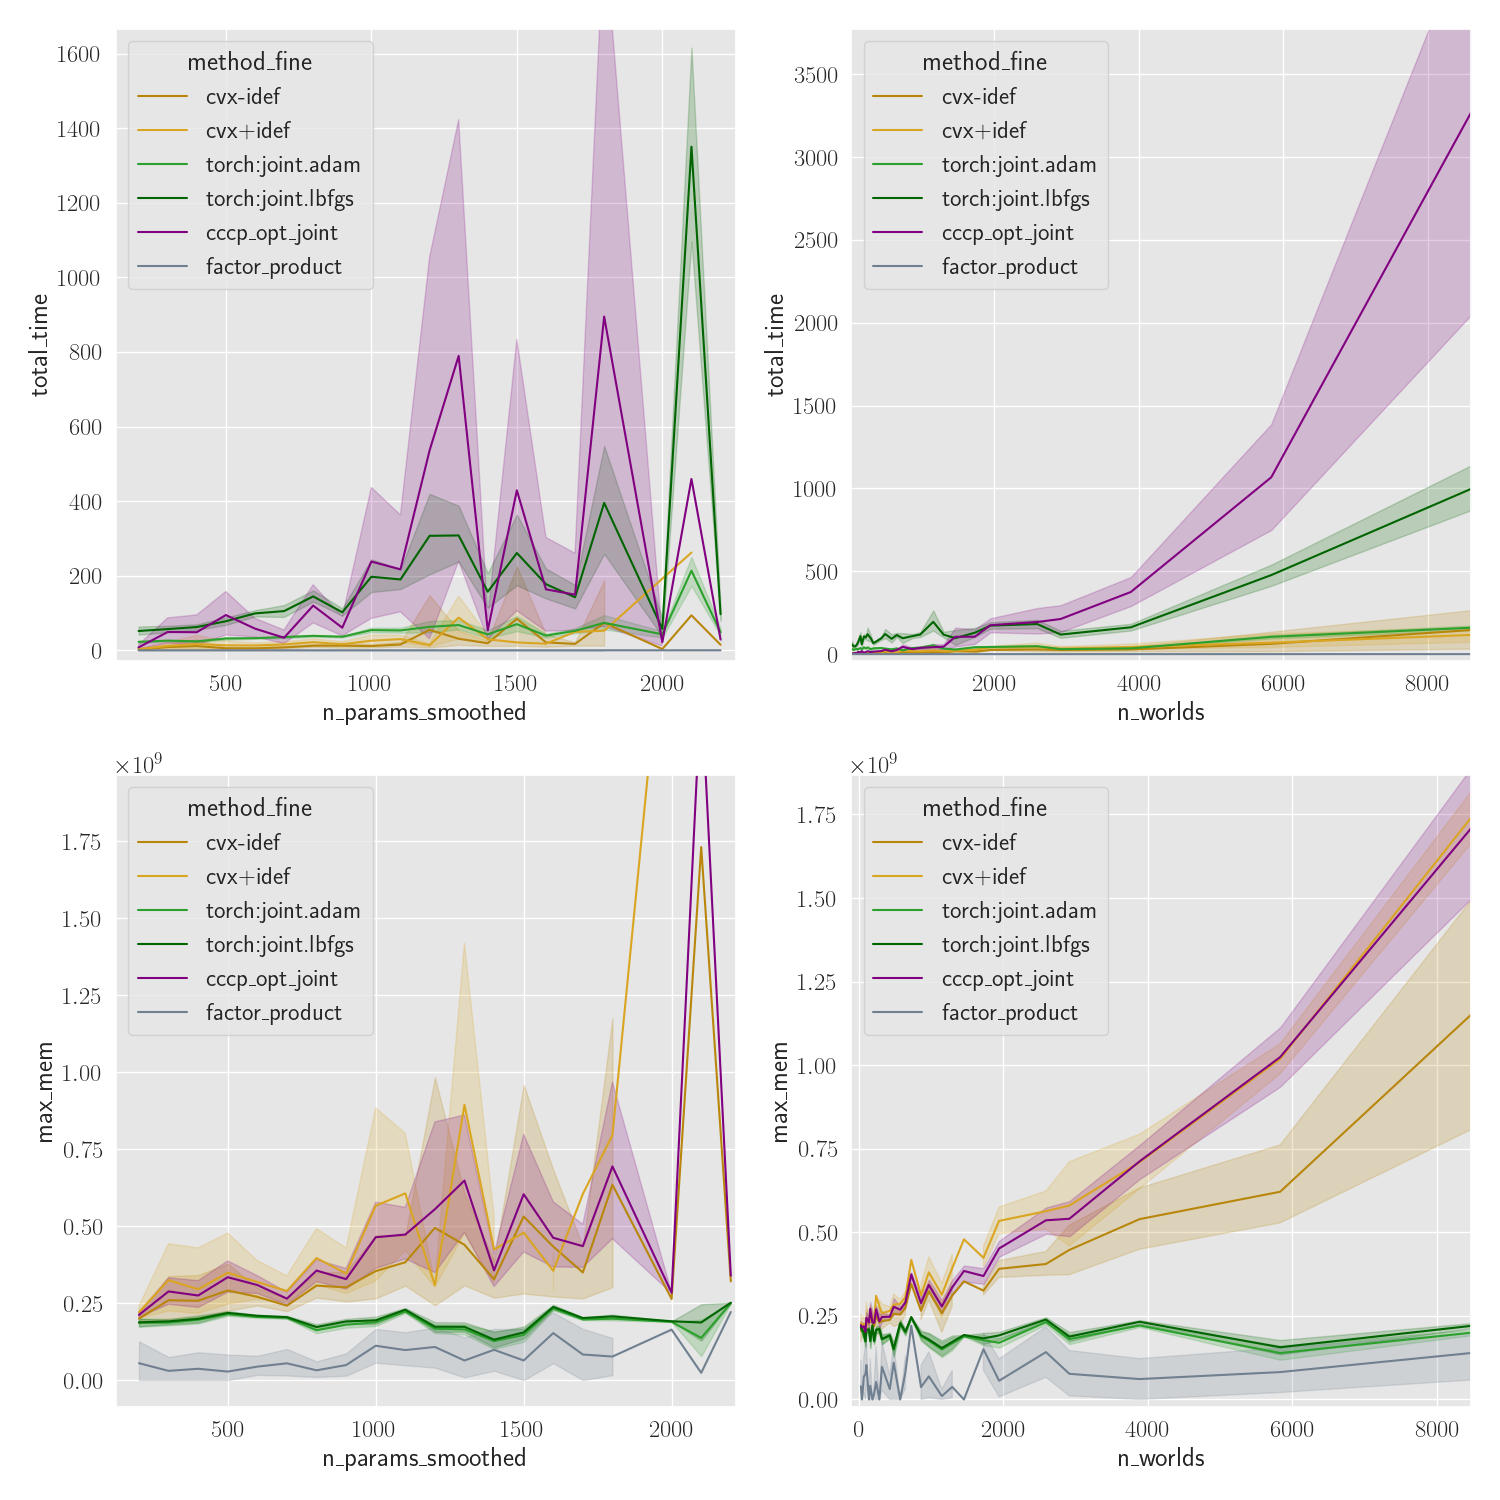
\includegraphics[width=\linewidth]{figs/rand-joint/resource-costs}
    \caption[More details: resource costs for joint-distribution optimization setting]{
    %\small
        Resource costs for the joint-distribution optimization setting of \cref{sec:inf-as-cvx-program}.
        We measure computation time (\texttt{total\_time}, top) and maximum memory usage (\texttt{max\_mem}, bottom) for the various optimization methods (by color), as the size of the PDG increases, as measured by the number of parameters in the PDG (\texttt{n\_params}$\,=\V\!\Ar$, left), and the size of a joint distribution over its variables (\texttt{n\_worlds}$\,=\V\!\X$, right).
        Note that the convex solvers for the 0 and $0^+$ semantics are significantly faster than LBFGS, and on par with Adam.
        However, all three convex-solver based approaches require significantly more memory than the black-box optimizers.
     }\label{fig:resources}
\end{figure}



\subsection{Synthetic Experiment: Comparison with Black-Box Optimizers, on Joint Distributions.} \label{sec:joint-expt-details}
\begin{wrapfigure}[14]{R}{4.8cm}
    \centering
    \vspace{-3ex}
    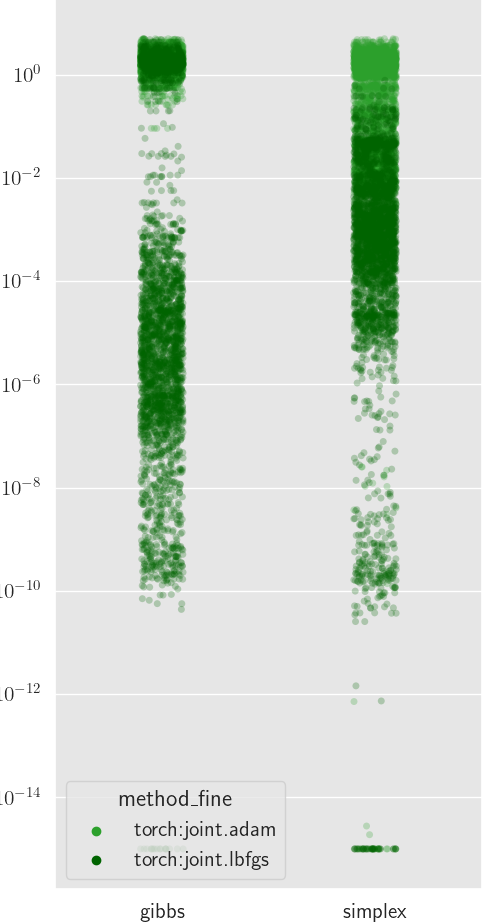
\includegraphics[width=4.5cm]{figs/rand-joint/representation}
    \captionsetup{format=plain}
    \caption{differences in performance between the Gibbs and simplex parameterizations of probabilities.}%
    \label{fig:representation}%
\end{wrapfigure}


Here is a more precise description of our first synthetic experiment,
on joint distributions, which contrasts the convex optimization approaches of \cref{sec:inf-as-cvx-program} with black-box optimizers.



\begin{itemize}
    \item generate 300 PDGs, each of which has the following quantities, to each of which we choose the following natural numbers uniformly at random:
    \begin{itemize}
        \item $N \in \{5,\ldots,9\}$ of variables
            (so that $\X := \{1, \ldots, N\}$),
        \item $V_X \in \{2, 3\}$ values per variable
            (so that $|\V X| = V_X$ for each $X \in \X$)
        \item $A \in \{7, \ldots, 14\}$ hyperarcs,
        each $a \in \{1, \ldots, A\} =: \Ar$ of which has
        \item $N^S_a \in \{0, 1, 2, 3\}$ sources, and
        \item $N^T_a \in \{1,2\}$ targets.
    \end{itemize}
    \item For each arc $a \in \Ar$, $N^S_a$ of the $N$ variables are choosen without replacement to be sources $S_a \subseteq N$, and $N^T_a$ of remaining variables are chosen to be targets. Finally, to each value of $S_a$ and $T_a$, a number $p_{a,s,t} \in [0,1]$ is chosen uniformly at random, and the cpd
    \[
     \p_a(\Tgt a {=} t \mid \Src a {=} s) =
        \frac{p_{a,s,t}}{\displaystyle\sum_{t' \in \V(T)} p_{a,s,t'}}
     \qquad\text{ is given by normalizing appropriately.}
    \]
    This defines a PDG $\dg M = (\X, \Ar, \mathbb P, \mat 1, \mat 1)$, that
    has $\balpha = \bbeta = \mat 1$, which will allow us to compare against
    belief propagation and other graphical models at $\gamma = 1$.
    The complexity of this PDG is summarized by two numbers:
    \begin{itemize}[nosep]
        \item \texttt{n\_params}$\,:= \V\!\Ar$, the total number of parameters in all cpds of $\dg M$, and
        \item \texttt{n\_worlds}$\,:= \V\!\X$, the dimension of joint distributions over $\dg M$'s variables.
    \end{itemize}
\end{itemize}

\begin{itemize}
    \item Run MOSEK on \eqref{prob:joint-inc} to find a distribution that minimizes $\OInc$; we refer to this method as \texttt{cvx-idef}
    \item Use the result to run MOSEK on \eqref{prob:joint+idef} to find the special distribution $\bbr{\dg M}^*_{0^+}$; we refer to this method as \texttt{cvx+idef}. These names are due to the fact that $\SDef$ is called $\IDef{}$ in previous work \parencite{pdg-aaai,one-true-loss};
    thus, this refers to using the convex solver to compute minimizers of $\OInc$ with and without considering $\IDef{}$.

    \item Run the \texttt{pytorch} baselines.
    Let $\theta = [\theta_{\mat x}]_{\mat x \in \V\!\X} \in \mathbb R^{\V\X}$ be a vector of optimization variables, and choose a representation of the joint distribution, either:
    \begin{align*}
        % \Big(\begin{array}{c}\text{renormalized}\\
        % \text{simplex}\end{array}\Big)\quad
        \mu_{\theta}(\mat x) &= \frac{\max\{\theta_{\mat x}, 0\} }
            {\sum_{\mat y \in \V\!\X}\max\{\theta_{\mat y}, 0\} }
        &(\text{ renormalized simplex }) \\
    \text{or}\qquad
    \mu_{\theta}(\mat x) &= \frac{\exp(\theta_{\mat x})}{\sum_{\mat y \in \V\!\X} \exp(\theta_{\mat y})} & (\text{Gibbs})
    % \qquad\quad\text{(see \cref{fig:representation})}
    \end{align*}
    See \cref{fig:representation} for a visual representation of the (relatively minor) effect of this choice. 
    \item
    For each value of the trade-off parameter 
    $\gamma \in \{0, 10^{-8}, 10^{-4}, 10^{-2}, 1\}$, and each learning rate $\texttt{lr} \in 1E-3, 1E-2, 1E-1, 1E0$, and each optimizer $\mathit{opt} \in \{\texttt{adam}, \texttt{L-BFGS}\}$,
    run $\mathit{opt}$ over the parameters $\theta$ to minimize $\bbr{\dg M}_\gamma(\mu_{\theta})$
     until convergence (or a maximum of 1500 iterations)

     \item We collect the following data about the resulting distribution and the process of computing it:
     \begin{itemize}[nosep]
         \item the total time taken to arrive at $\mu$;
         \item the maximum memory taken by the process computing $\mu$;
         \item the objective and its component values:
         \vspace{-1ex}
         \[
            \begin{array}{c}
            \texttt{inc} := \SDef_{\dg M}(\mu), \\
            \qquad \texttt{idef} := \SDef_{\dg M}(\mu),
            \end{array}
            \qquad \texttt{obj} := \OInc_{\dg M}(\mu) + \gamma \SDef_{\dg M}(\mu) = \bbr{\dg M}_\gamma(\mu)
        \]
     \end{itemize}
\end{itemize}



The numbers can then be recreated by running our experimental script as follows:
\begin{verbatim}
python random_expts.py -N 300 -n 5 9 -e 7 14 -v 2 3
    --ozrs lbfgs adam
    --learning-rates 1E0 1E-1 1E-2 1E-3
    --gammas 0 1E-8 1E-4 1E-2 1E0
    --num-cores 20
    --data-dir random-joint-data
\end{verbatim}
which creates a folder called \verb|random-joint-data|,
and fills it with \verb|.mpt| files corresponding to each distribution
and the method / parameters that gave rise to it.

\textbf{Analyzing the Results.}
Look at  \cref{fig:resources}.  Our theoretical analysis, and in particular the proof of \cref{lem:cluster-inc-polytime}, suggest that the magnitudes of $\V\!\X$ and $\V\!\Ar$ play similar roles in the asymptotic complexity of PDG inference.
Our experiments reveal that, at least for random PDGs, the number of worlds is the far more important of the two; observe how much more variation there is on the left side of the figure than the right---and now note that the left side has been smoothed, while the right side has not.
The black-box py-torch based approaches clearly have an edge in that they can handle larger models, as evidenced by the cut-offs on the right-hand side of \cref{fig:gap-resource-fine-old}, when with 5GB memory.

Note that the exponential-cone-based methods for the observational limit (gold) are actually faster than L-BFGS (the black-box optimizer with the lowest gap), and also seem to be growing at a slower rate.
However, they use significantly more memory, and cannot handle large models.
In addition to being faster, our techniques also seem to be more precise; they achieve objective values that are consistently much better than the black-box methods.


Now look at \cref{fig:joint-gap-vs-time-by-gamma},
which contains a break-down of the information in \cref{fig:joint-gap-time}. The bottom half of the figure is just the same information, but with each value of $\gamma$ separated out, so that the special cases of the factor product and $0^+$ inference become clear, while the top half shows why it's more important to look at the gap than the actual objective value for these random PDGs.
\Cref{fig:joint-gap-vs-time-by-gamma} also makes it clearer how larger problems take longer, and especially so for \texttt{cccp} (violet), which solves the most complex version of the problem \eqref{prob:joint-small-gamma}.

\begin{figure}
    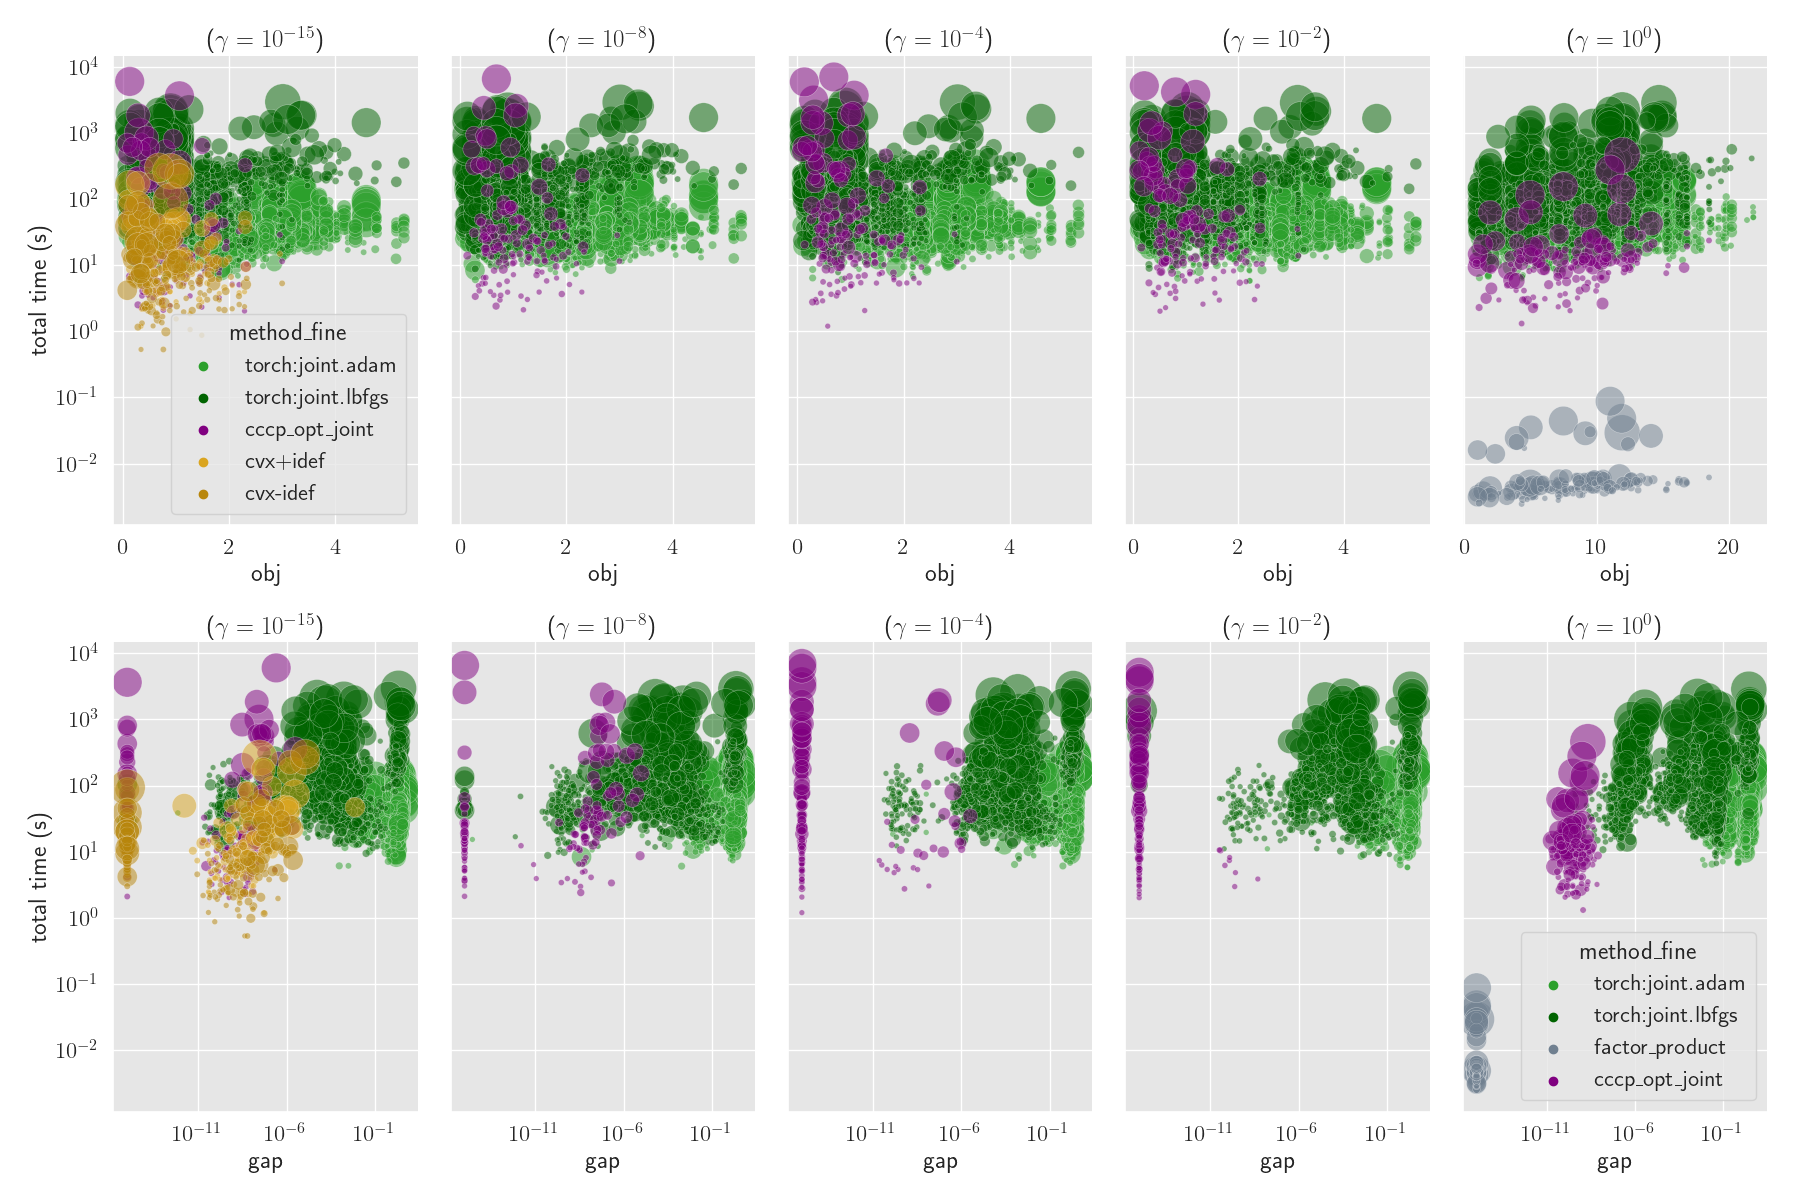
\includegraphics[height=0.45\textheight]{figs/rand-joint/gap-vs-time-by-gamma}
    \caption[A disaggregated version of \cref*{fig:joint-gap-time}]{\small
        An un-compressed version of the information in \cref{fig:joint-gap-time}, that groups by the value of $\gamma$, and also gives the absolute values of the objectives (top row) in addition to the relative gaps (bottom row).
    }\label{fig:joint-gap-vs-time-by-gamma}
\end{figure}




% \discard{\begin{figure}
%     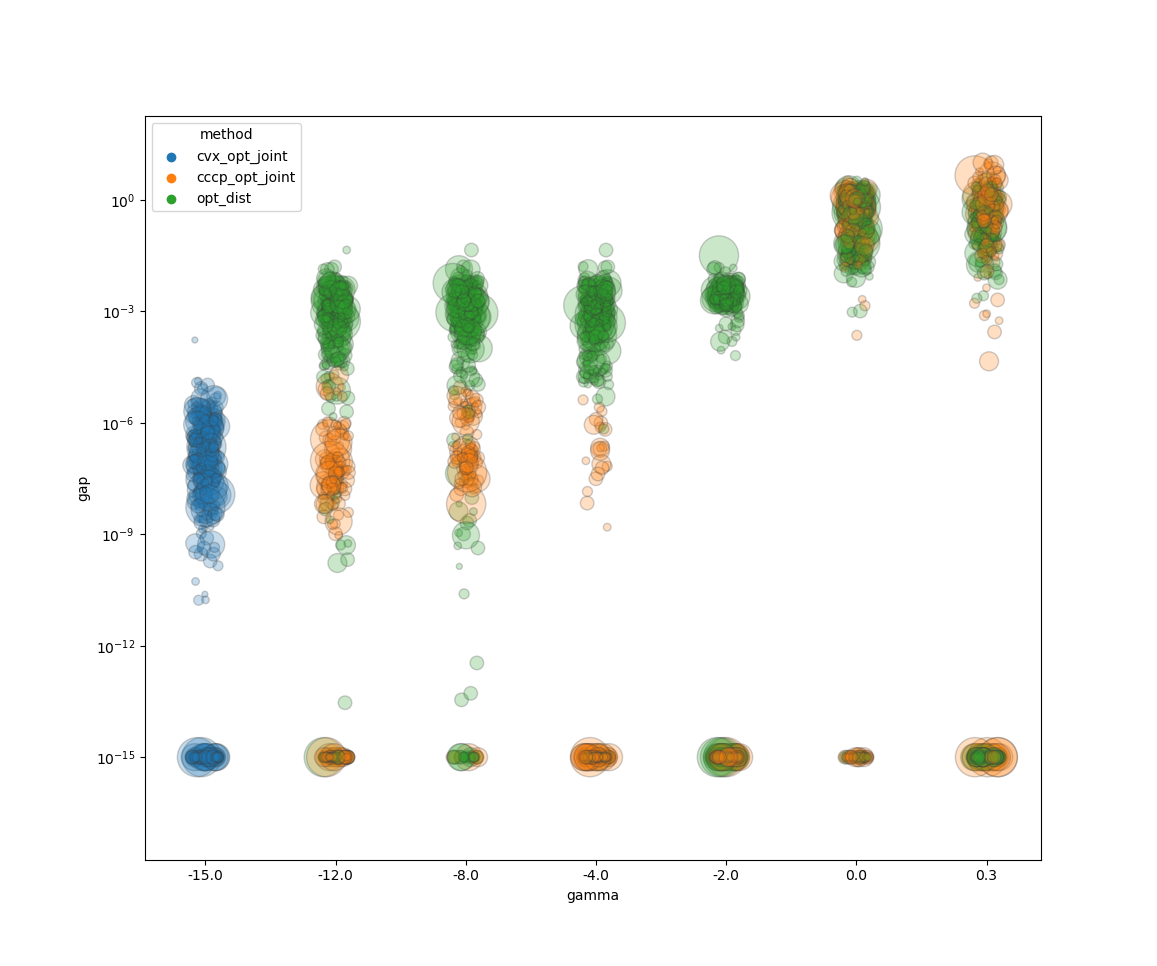
\includegraphics[height=0.45\textheight]{figs/gamma-vs-gap-bettergap}
%     \caption{
%         A graph of the gap (the difference between the attained objective value, and the best objective value obtained across all methods for that value of $\gamma$),
%         as $\gamma$ varies. The x-axis is $\log_{10} ( \gamma + 10^{-15})$.
%         As before, colors indicate the optimization method; here blue corresponds to \eqref{prob:joint+idef}, while orange corresponds to \eqref{prob:joint-small-gamma}, and green, as before, corresponds to all optimization baselines.
%         The size of the circle illustrates the relative number of worlds.
%         See \cref{fig:gamma-v-gap-fine} for a more detailed breakdown.
%     }\label{fig:gamma-v-gap}
% \end{figure}}


\begin{figure}
    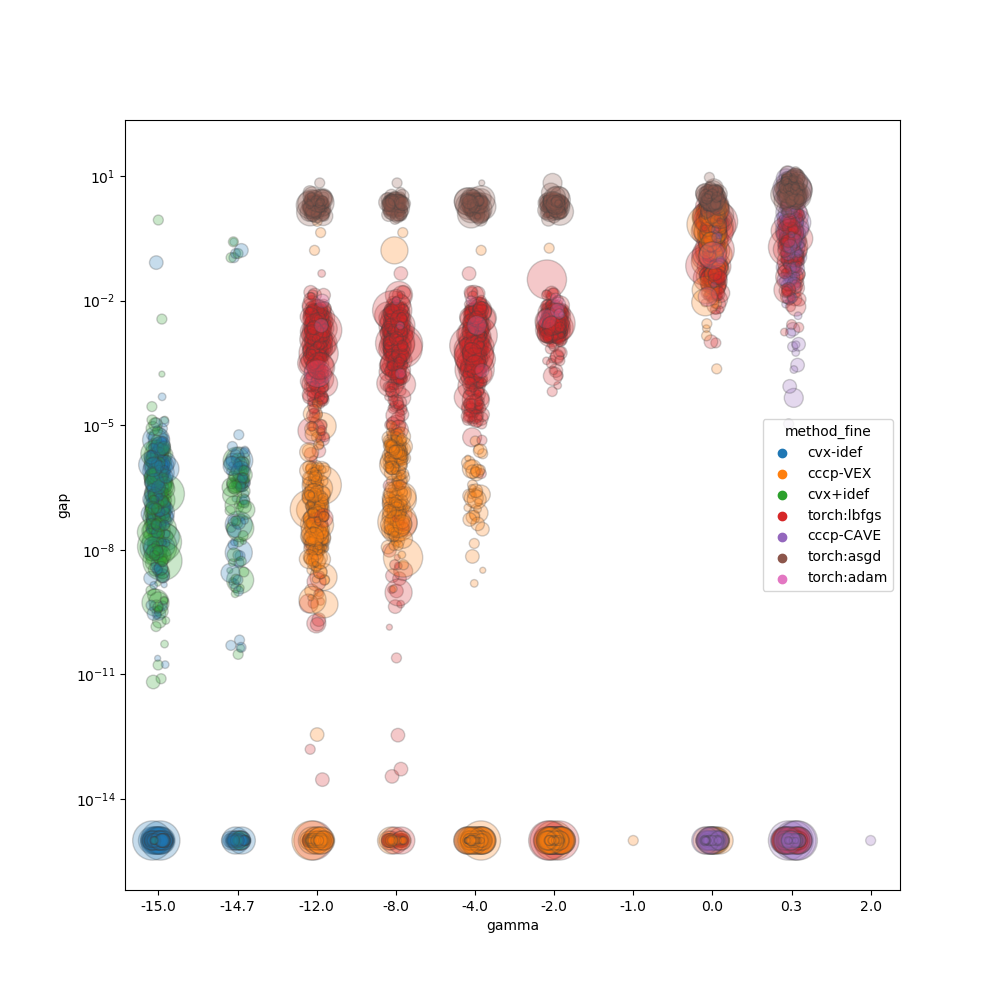
\includegraphics[width=\linewidth]{figs/2}
    \caption[
        Plot of the accuracy gap for inference methods and baselines, for various values of $\gamma$.
    ]{
        A graph of the gap (the difference between the attained objective value, and the best objective value obtained across all methods for that value of $\gamma$),
        as $\gamma$ varies. The x-axis is $\log_{10} ( \gamma + 10^{-15})$.
        As before, colors indicate the optimization method, and
        the size of the circle illustrates the number of optimization variables (i.e., the number of possible worlds).
        \texttt{cvx-idef} corresponds to just solving \eqref{prob:joint-inc}, and \texttt{cvx+idef} corresponds to then solving problem \eqref{prob:joint+idef} afterwards.
        The CCCP runs are split into regimes where the entire problem is convex ($\gamma \le 1$, labeled \texttt{cccp-VEX}), and the entire problem is concave ($\gamma > 1$, labeled \texttt{cccp-CAVE}).
        The optimization approaches \texttt{opt\_dist} are split into three different optimizers: LBFGS, Adam, and also a third one that
        performs relatively poorly: accelerated gradient descent.
        Note that for small $\gamma$, the exponential-cone based methods significantly outperform the gradient-based ones.
    }\label{fig:gamma-v-gap-fine}
\end{figure}


\subsection{Synthetic Experiment: Comparing with Black-Box Optimizers, on \AcTree s} \label{sec:clus-expt-details}

\begin{figure}
    \centering
    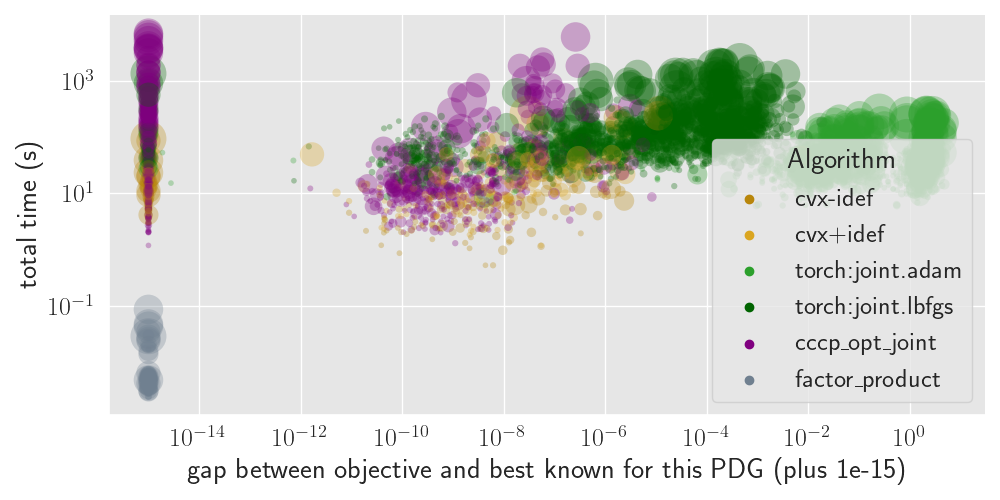
\includegraphics[width=0.67\linewidth]{figs/rand-clus/gap-vs-time}
    \caption[Objective gap vs time in the cluster setting; shows more separation]
        {An analogue of \cref{fig:joint-gap-time}, for the cluster setting.
    Note that there is even more separation between the exponential-cone based approaches, and the black-box optimization based ones.
    The new grey points on the bottom correspond to belief propagation, which is both faster and typically the most accurate.}
    \label{fig:clus-gap-vs-time--appendix}
\end{figure}
\begin{figure}
    \centering
    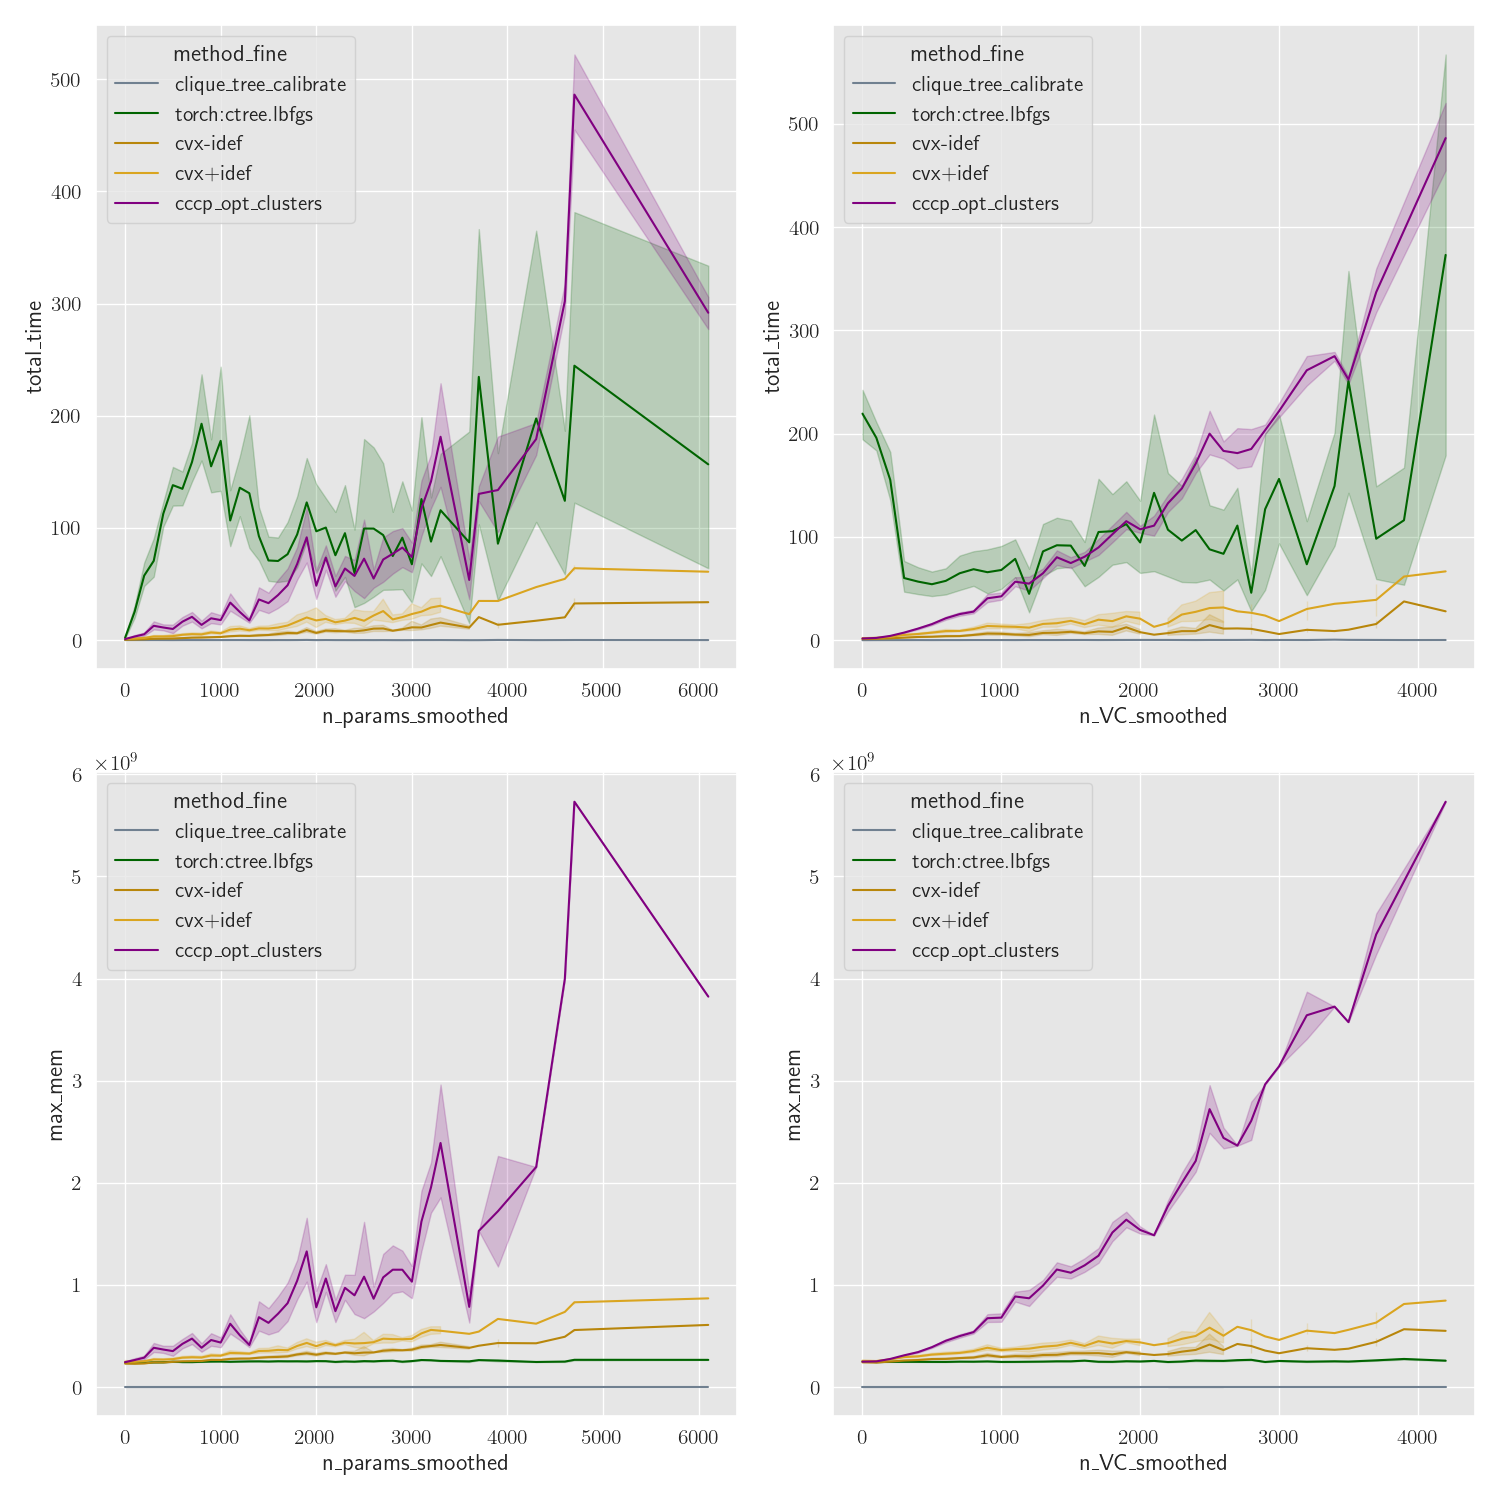
\includegraphics[width=0.67\linewidth]{figs/rand-clus/resource-costs}
    \caption[Resource costs for the cluster setting.]
        {Resource costs for the cluster setting. Once again, the $\OInc$-optimizing exponential cone methods are in gold, the small-gamma and CCCP is in violet, and the baselines are in green. The bottom line is belief propagation, which is significantly faster and requires very little memory, but also only gives the correct answer under very specific circumstances.}
    \label{fig:clus-resource-costs}
\end{figure}


\begin{enumerate}
    \item Choose a number of variables $N \in \{ 8, \ldots, 32 \}$, and a treewidth $k \in \{1, \ldots, 4\}$ uniformly at random.
    Then draw a random $k$-tree and corresponding tree of clusters $(\C, \mathcal T)$, as follows:
    \begin{enumerate}
        \item Initialize $G \gets K_{k+1}$ to a complete graph on $k+1$ vertices, and $\C \gets\{ K_{k+1} \}$ to be set containing a single cluster, and $\mathcal T\gets \emptyset$.
        \item Until there are $N$ vertices: add a new vertex $v$ to $G$, then randomly select a size $k$-clique (fully-connected subgraph) $U \subset G$, and add edges between $v$ and every vertex $u \in U$.
        Add $U \cup \{v\}$ to $\C$, and add edges to every other cluster $C \in \C$ such that $U \subset C$.
    \end{enumerate}
    \item Draw the same parameters $V_X \in \{2,3\}$, $A \in \{8, \cdots, 120\}$, $N_a^S \in \{0,1,2,3\}$, and $N^{T}\in \{1,2\}$
    as in \cref{sec:joint-expt-details} uniformly at random.
    While $N_a^S + N^T_a > k+1$, for any $a$, resample $N_a^S$ and $N_a^T$.

    \item Form a PDG whose structure $\Ar$ can be decomposed by $(\C, \cal T)$, as follows:
    for each edge $a \in \Ar$, sample a cluster $C \in \C$ uniformly at random; then select $N_a^S$ nodes from that cluster without replacement as sources, and $N_a^T$ nodes as targets; this is possible because each cluster has $k+1$ nodes, and $N_a^S + N_a^T \le k+1$ by construction.
    \item Fill in the probabilities by drawing uniform random numbers and re-normalizing, just as before, to form a PDG $\dg M$

    \item The black-box optimization baselines work in much the same way also, although now the optimization variables include not one distribution $\mu$ but a collection $\bmu$ of them;
    this time, we use only the simplex representation of $\bmu_\theta$.
    More importantly, we want these clusters to share appropriate marginals; to encourage this, we add a terms to the loss function, so overall, it is
    \[
        \ell(\theta) := \bbr{\dg M}_{\gamma}(\bmu_{\theta})  + \sum_{\mathclap{C{-}D \in \mathcal T}}\exp \!\left(\sum_{w \in \V(C\cap D)\!\!\!\!} \big(\mu_C(C\cap D{=}w) - \mu_D(C \cap D {=}w)\big)^2 \right) - 1.
    \]
    This is admittedly pretty ad-hoc; the point is just that it is zero and does not contribute to the gradient if $\bmu_\theta$ is calibrated, and otherwise quickly becomes overwhelmingly important.
\end{enumerate}

\textbf{Analyzing the Results.}
Observe in \cref{fig:clus-gap-vs-time} that the separation between the \actree\ convex solver and the black-box algorithms is even more distinct. This is because, in this case, the penalty for violating constraints was too small, and the optimization effort was largely wiped out by the calibration before evaluation.


\begin{figure}
    \centering
    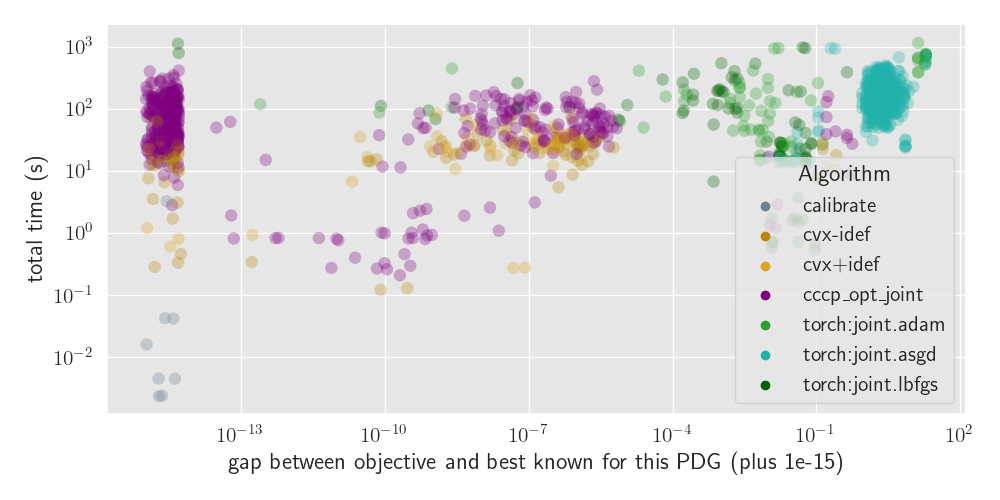
\includegraphics[width=0.7\textwidth]{figs/bn/gap-v-time}
    \caption{Gap vs inference time for the small PDGs in the \href{https://www.bnlearn.com/bnrepository/}{\texttt{bnlearn}} repository}
    \label{fig:bn-gap-v-time}
\end{figure}

This illustrates another general advantage that the convex solver has over black-box optimizers: it is much less brittle and reliant and exactly tuning parameters correctly. Note that even in this minimal example, there were many hyper-parameters that require tuning:
the regularization strengths that enforce soft constraints (\actree\ calibration, normalization), as well as learning rate, not to mention
various other structural choices: the optimizer, the representation of the distribution, and the maximum number of iterations, none of which are clear-cut choices, but rather require first being tuned to the data.
While the convex solver does have internal parameters (tolerances and such) these do not need to be tuned to the problem under normal circumstances.

\subsection{Comparing to Belief Propagation, on \AcTree s.}
    \label{sec:bn-expt-details}
 Since PDGs generalize other graphical models, one might wonder how our method stacks up against algorithms tailored to the more traditional models. In brief: our algorithm is much slower, and only handle much smaller networks.
 Concretely, our methods can handle all of the ``small'' networks, and some of the ``medium'' ones, from the \href{https://www.bnlearn.com/bnrepository/}{\texttt{bnlearn}} repository.
  In these cases, we have verified that the two methods yield the same results.
  \Cref{fig:bn-gap-v-time} contains the analogue of \cref{fig:joint-gap-time,fig:clus-gap-vs-time}
  for the Bayesian Nets. This graph looks qualitatively quite similar to the other graphs we've seen, suggesting that the results in our synthetic experiments hold more broadly for small real-world models as well.




 \begin{figure}
     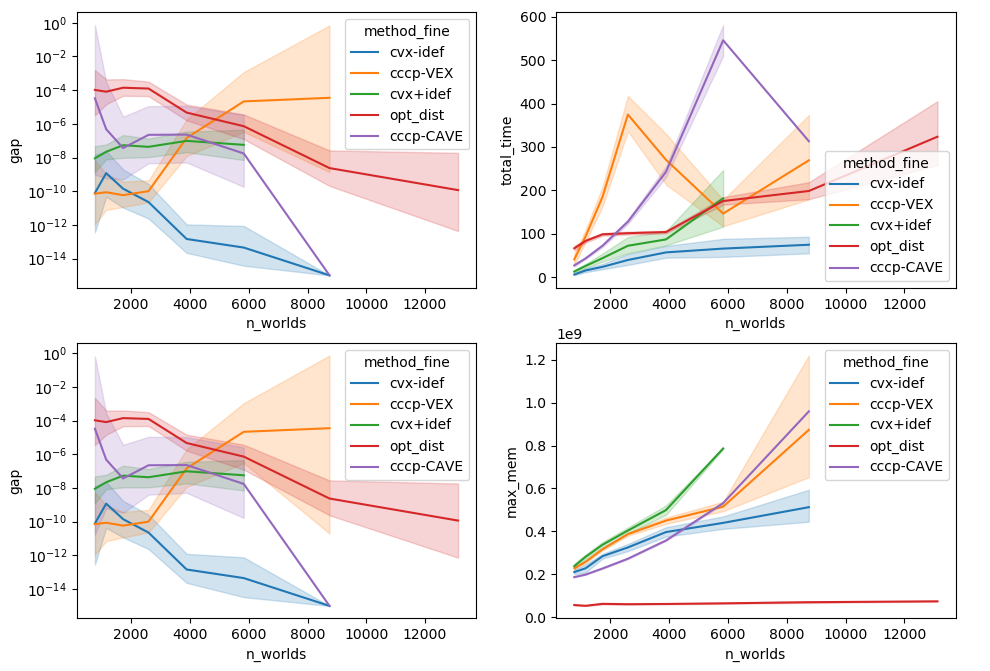
\includegraphics[height=0.45\textheight]{figs/1}
     \caption{
         A variant of \cref{fig:resources}, with
         with gap (accuracy) information on the left, and slightly different parameter settings.
     }\label{fig:gap-resource-fine-old}
 \end{figure}


\end{subappendices}

\chapter{Lower Bounds, and The Deep Connection between Inconsistency and Inference}
        \label{chap:inc-infer-connection}
\colorlet{proofmatt}{white}


On one hand, PDGs are powerful modeling tools, and representations of uncertainty.
On the other, PDGs are universal loss functions. 
This chapter describes a deep connection between two roles of PDGs. 
We start with a suggestive observation: that the semantics by which PDGs specify a distribution is equivalent to the semantics that simply evaluates a PDG's degree of inconsistency (\cref{sec:semantic-connection}). 
We then build on this semantic connection by describing a surprisingly strong algorithmic one: an inconsistency oracle can be used to perform inference (\cref{sec:deeper-connection-overview}) in almost-linear time. 
% To do this precisely, we must also formally describe the problems of approximate inference and inconsistency (\cref{sec:approximate-inference}).
% We prove  (rather substantial) proof to \cref{proofs:the-reductions}.
% In this sense, precisely quantifying one's inconsistencies is no easier than optimally resolving them.  
Thus, the two views of PDGs are essentially equivalent---not only semantically, but algorithmically as well.
%
\newmaterial{%
    % This 
% The result is a deep and rather philosophical conclusion:
This leads to a philosophically profound result: precisely quantifying one's degree of inconsistency is no easier than optimally resolving those inconsistencies. 
}%

To get there, we first need to formally describe the two computational problems of interest (\cref{sec:approximate-inference}) as approximate inference problems,
which allows us to also
formally finish the upper bounds developped in \cref{chap:infer}.

 
% \section{A Semantic Connection}
\section{A Semantic Connection}
    \label{sec:semantic-connection}

% Recall that the inconsistency of a PDG is the score of its best-scoring distribution:
% \[
%     \aar{\dg M}_\gamma := \inf_{\mu \in \Delta \V\!\X} \bbr{\dg M}_\gamma(\mu).
% \]
Recall that we defined the inconsistency $\aar{ \,\cdot\, }$ of a PDG is the score of its best-scoring distribution.
Although we defined
$\aar{ \,\cdot\, }$
in terms of the scoring-function semantics (\ref{eq:inc-scoring-semantic-equivalence}, left), it worth noting that the reverse is also possible: the scoring function can be defined in terms of inconsistency (\ref{eq:inc-scoring-semantic-equivalence}, right).
%
% \begin{prop}
    % For all $\gamma$,
    % $
    % \[
\begin{equation}
    \aar{\dg M}_\gamma = \inf_{\mu \in \Delta \V\!\X} \bbr{\dg M}_\gamma(\mu)
    \qquad
    \qquad
    \bbr{\dg M}_\gamma = \aar{\dg M + \mu!}_\gamma
    ~.
    \label{eq:inc-scoring-semantic-equivalence} 
\end{equation}
    % \]
    % $
% \end{prop}
% As a result

Although the technical details are not surprising, this fact seems quite surprising if we take a few steps back and reflect on its meaning at a higher level.
In general, a function $f : X \times Y \to \mathbb R$ typically contains strictly more information than its minimizers $(x \mapsto \argmin_y f(x,y) \subseteq Y) : X \to 2^Y$, which in turn one typically thinks of as containing more information than its minimum value 
\[
\min_Y f = (x \mapsto \min_y f(x,y)) : X \to \mathbb R. 
\]
In this case, however, when we take $X$ to be the set of PDGs, $Y$ to be the set of joint distributions, and $f$ to be the scoring function, $\min_Y f$ is equivalent to $f$ itself, in the sense that either can be derived from the other. 

So, semantically, the PDG inconsistency measure is equivalent to the full scoring function. 
Despite returning only a single number, the PDG inconsistency $\aar{\,\cdot\,}_\gamma$
encodes so much information that the optimal (set of) distribution(s) of a PDG \cref{sec:semantics} can be derived from it. 
% It can be computationally challenging (if even possible) to calculate $\min_Y f$ from $f$, 

When a single number encodes so much information,
    it is often because that information has been heavily compressed, 
    and the drawback is that a lot of calculation is necessary to recover the original information.
But, perhaps surprisingly, in this case it appears that the compressed form is not only more simpler and more compact, but also easier to use.  
To calculate $\aar{\,\cdot\,}_\gamma$ from $\bbr{\,\cdot\,}_\gamma$
requires solving an optimization problem over an enormous space,
while the calculating $\bbr{\,\cdot\,}_\gamma$ from $\aar{\,\cdot\,}_\gamma$
requires only passing the function argument to the PDG and a single evaluation \eqref{eq:inc-scoring-semantic-equivalence}. 
% What's even more interesting is that 
Yet recovering the scoring function from inconsistency is only the beginning.
Once we define the computational problems at hand precisely
    (which we do in \cref{sec:approximate-inference}),
it will turn out that even PDG inference can be done in linear
    time with an inconsistency oracle \cref{sec:deeper-connection-overview}.
All of this suggests at a theoretical level something we
    illustrated at length in \cref{chap:one-true-loss}:
    that calculating the degree of inconsistency is a fundemental problem, that can be used to solve other problems. 

    
% Conceptually, this result is not so different from the relation between a factor graph and its partition function 
Indeed, as previously mentioned (e.g., in \cref{sec:free-energy-fg-inc}),
    a factor graph (a special case of a PDG, by \cref{theorem:fg-is-pdg})
    is associated with a similarly important number, called its \emph{free energy} or \emph{log partition function} (which is the inconsistency of this factor graph when viewed as a PDG, by \cref{prop:fg-inconsistency-is-partition-function}).
Calculating this number is computationally difficult, but if it is known, then inference becomes far easier \citep{ma2013estimating,KF09}. 
% The results of this chapter de-mystify the nature of this relationship
This chapter will clarify the nature of this relationship, generalize it to a far wider class of probabilistic models, and significantly strengthen the reduction.
More precisely, we will show that an inconsistency oracle on its own can be used to perform inference in time linear in the length of its required output length.

This will make precise a rather profound fact: not only is it difficult to see one's inconsistencies, but in fact precisely quantifying them is no easier than optimally resolving them.

% \chapter{The Deep Connection between Inference and Inconsistency}
% \section{Approximation}
\section{The Computational Complexity of (Approximate) Inference and Inconsistency Calculation}
    \label{sec:approximate-inference}

\def\ApproxPDGInfer{\textsf{APPROX-PDG-INFER}}
\def\ApproxPDGInc{\textsf{APPROX-CALC-INC}}
\def\ApproxInferUniq{\textsf{APPROX-INFER-CVX}}

Most work in graphical models works with abstract representations of real numbers, assuming that arithmetic (e.g., addition and multiplication of numbers) can be done in constant time. 
This assumption has several enormous advantages. 
\begin{enumerate}
\item 
It simplifies things a great deal, and puts the focus where it should be: on the important aspects of the algorithm, rather than the details of numerical representations.
\item 
It is essentially the right model of computational complexity in practice, given the we typically cache out numerical computations with floating point represntations in hardware, which approximately have this complexity.
\item 
Finally, the assumption typically does not impact theoretical results, because (with a great deal of difficult and uninteresting work) one can often assume that all parameters are rational numbers, and then show that the the calculations can be done just as before with a small overhead.
\end{enumerate}

Unfortunately, and for a very superficial reason, the final point does not apply to PDGs.
% ---and therefore if we are to speak precisely about computational complexity, we must talk about \emph{approximate} inference. 
While \cref{theorem:main} gives us a way of doing inference to machine precision in polynomial time, which is the typical use case of an exact algorithm, it is not technically an exact inference algorithm.
Indeed, if we use binary representations of numbers, exact inference for PDGs is technically not possible in finite time: in a PDG, the exact answer to an inference query may be an irrational number (even if all components of $\mathbb P$,$\balpha$, and $\bbeta$ are rational).
Therefore, in order to say something precise about the computational complexity of inference, the problem we formulate precisely must be that of \emph{approximate} inference. 

\begin{defn}[approximate PDG inference]
    An instance of problem \ApproxPDGInfer\ 
    is a tuple $(\dg M, \gamma, Q, \epsilon)$, where
    $\dg M$ is a PDG with variables $\X$, $\gamma \in \{0^+\} \cup [0, \infty]$
    is the relative importance of structural information,
    $Q$ is a conditional probability query of the form
    ``$\Pr(Y{=}y|X{=}x) = ?$'', where $X,Y \subseteq \X$ and $(x,y) \in \V(X,Y)$,
    and $\epsilon > 0$ is the precision desired for the answer.
    A solution to this problem instance is a pair of numbers
    $(r^-, r^+)$
    such that
    \begin{align*}
        r^- &\le \inf_{\mu \in \bbr{\scalebox{0.7}{$\dg M$}}^*_\gamma} \mu(Y{=}y | X{=}x) \le r^- + \epsilon \\
        \text{and} \qquad
        r^+ &\ge \sup_{\mu \in \bbr{\scalebox{0.7}{$\dg M$}}^*_\gamma} \mu(Y{=}y | X{=}x) \ge r^+ - \epsilon. 
        \qedhere
    \end{align*}
\end{defn}

The problem we solved in \cref{sec:inf-as-cvx-program,sec:clique-tree-expcone}
is the special case in which $\dg M$ is assumed to be proper and $\gamma \in \{0^+\} \cup (0, \min_a \frac{\beta_a}{\alpha_a})$.  This is enough to ensure there is a unique optimal distribution $\mu^* \in \bbr{\dg M}^*_\gamma$, with respect to which we must answer all queries.  In this case, the definition above 
essentially amounts to providing a single
number $p$ such that $p-\epsilon \le \mu^*(Y{=}y|X{=}x) \le p+\epsilon$.  
We call this easier subproblem \ApproxInferUniq.
We will also be interested in the unconditional variants of both inference
problems, in which  
    no additional evidence is supplied (i.e., $X = \emptyset$). 
We now define the analogous problem of approximately calculating a PDG's  degree of inconsistency. 

\begin{defn}[approximate inconsistency calculation]
    An instance of problem 
    \ApproxPDGInc\ 
    is a triple $(\dg M, \gamma, \epsilon)$, where
    $\dg M$ is a PDG, $\gamma \ge 0$, and $\epsilon > 0$ is the desired precision. 
    A solution to this problem instance is 
    a number $r$ such that $|\aar{\dg M}_\gamma - r | < \epsilon$.
\end{defn}

The interior point method behind \cref{theorem:main} solves \ApproxPDGInc\ 
    in the process of finding a \actree\ for inference. 
But, technically, it does not solve \ApproxPDGInfer. 
A solution to \ApproxPDGInfer\ is
a conditional probability, not a \cactree.
While a \cactree\ does allow us to compute conditional
probabilities, 
an $\epsilon$-close \actree\ does not give us $\epsilon$-close answers
    to probabilistic queries, especially those conditioned on improbable events (i.e., finding $\Pr(Y{=}y|X{=}x)$ when $\Pr(X{=}x) \approx 0$).
Nevertheless, because precision is so cheap,
the interior point method behind \cref{theorem:main}
can still be used as a subroutine to solve \ApproxInferUniq. 

\begin{linked}{theorem}{approx-infer}
\ApproxInferUniq\ can be solved in
\def\mustar{\mu^{\mskip-2mu*\!}}
\begin{align*}
    \tilde O \pqty[\bigg]{ \! (N\!+\!A)^4 V^{4(T+1)}
    \log \frac1{\epsilon \mustar(x)\!}
    \Big[
          \log \frac{\beta^{\max}\!}{\beta^{\min}\!} 
           + \log \frac1{\epsilon  \mustar(x)} 
    \Big]\! }
\end{align*}
time,
\onlyfirsttime{\unskip\footnote{%
   \label{note:<4possible}%
   At the cost of substantial overhead and engineering effort, the exponent $4$ can be reduced to 2.872, by appeal to \textcite{skajaa2015homogeneous} and the current best matrix multiplication algorithm \parencite[$O(n^{2.372})$]{duan2022faster} to invert $n{\times} n$ linear systems. 
}}
where $\mustar(x)$ is the probability of the event $X{=}x$ in the optimal
distribution $\mu^*$, 
 $\beta^{\max} := \max_{{a \in \Ar}} \beta_a$ is the largest observational confidence, 
\[
\text{and}\qquad
\beta^{\min} := 
\begin{cases}
    ~\displaystyle\min_{a \in \Ar} \{ \beta_a : \beta_a > 0\}& \text{if}~ \gamma = 0^+\\[-0.5ex]
    ~\hfill\gamma~~ & \text{if}~ \gamma > 0~~\text{.}
\end{cases}
\]
\end{linked}

The factor of $\log(\nf1{\mu^*\!(x)})$ is unusual, 
but even exact inference algorithms typically must write down $\mu^*(X{=}x)$
on the way to calculating $\mu^*(Y{=}x|X{=}x)$, which implicitly incurs 
a cost of at least $\log(\nf1{\mu^*\!(x)})$. 
A Bayesian network with $N$ variables in which cpds are articulated to precision $k$
can have nonzero marginal probabilities as small as $2^{- N k}$,
    in which case the additional worst case overhead for small probabilities is linear. 
We conjecture that it is not possible to form smaller marginal probabilities with PDGs, although the question remains open. 
Algorithmically speaking,
\cref{theorem:approx-infer} extends \cref{theorem:main} 
in three key ways. 

\begin{enumerate}
\item We must request additional precision 
    to ensure that the marginal probabilities deviate at most $\epsilon$
    from the true ones.  This sense of of approximation effectively
    bounds the $\ell_1$ norm of $\bmu^* - \bmu$,
    while \cref{theorem:main} (a) bounds it $\ell_2$ norm and
    (b) bounds its $\ell_\infty$ norm.

\item We must introduce a loop to refine precision until we have a suitably precise estimate of $\Pr(X{=}x)$.

\item Rather than directly dividing our estimate of $\Pr(Y{=}y,X{=}x)$ by our estimate of $\Pr(X{=}x)$, we calculate something slightly more stable. 
\end{enumerate}

See the proof for details. 
One immediate corollary of \cref{theorem:approx-infer} is that
\ApproxInferUniq\ $\subseteq \mathsf{EXP}$, without the assumption of bounded treewidth.


It may be worth noting that there is at least one instance in the literature where \emph{approximate} Bayesian Network (BN) inference is tractable for a subclass of models other than those of bounded treewidth: \textcite{Dagum-Luby-approximate} give a randomized algorithm for the special class of Bayesian Networks that do not have extreme conditional probabilities. Specifically they show that, assuming a network with $N$ nodes, the inference problem is in $\mathsf{RP}(N, \nf1\epsilon)$. 
In addition to restricting to a different class of models (bounded conditional probabilities, but not bounded treewidth), their approximation 
    algorithm in another significant respect: it is polynomial in $\nf1\epsilon$, rather than in $\log(\nf1\epsilon)$. 
Thus, the time it requires is exponential with respect to the number of requested digits,
    while our algorithm takes linear time.

Because PDGs generalize BNs, approximate inference
for PDGs is at least as hard as it is for BNs.

\begin{prop}[\parencite{roth-hardness-1996}]
        \label{bn-sharp-P-hard}
    \ApproxPDGInfer\ is \#P-hard. 
\end{prop}

Thus, the exponential time of \cref{theorem:approx-infer}
    is the best we could have hoped for, in the general case.  
The argument is due to \textcite{roth-hardness-1996}, 
although we have altered it somewhat. 


\section{A Deeper, Computational Connection}
    \label{sec:deeper-connection-overview}

Our approach to $\zogamma$-inference computes
$\aar{\dg M}_\gamma$ as a side effect.
But suppose that we were interested in calculating only this inconsistency.
Might there be a more direct, asymptotically easier way 
to do so? In general, the answer is no.

\begin{linked}{theorem}{consistent-NP-hard}
    \label{prop:sharp-p-hard}
    \begin{enumerate}[label={\rm{(\alph*)}}]
    \item Determining whether 
    there is a distribution
    that satisfies all cpds of a PDG
    is NP-hard.
    \item Calculating a PDG's degree of inconsistency (exactly) is \#P hard.
    \item \ApproxPDGInc\ is \#P hard,
        even for fixed $\gamma \ge 0$ and $\epsilon > 0$.
    \end{enumerate}
\end{linked}

% \textcite{pdg-aaai}'s original approach to  
Historically, our original approach to inferring the probability of 
$Y$ in a PDG $\dg M$ was to minimize their combined inconsistency \citep{pdg-aaai}. 
The idea is to add a hypothesis distribution $h(Y)$ to $\dg M$, and 
adjust $h$ to minimize the overall inconsistency $\aar{\dg M + h}_\gamma$.
Parts (b) and (c) of \cref{prop:sharp-p-hard} significantly undermine this approach, because even just calculating $\aar{\dg M + h}_\gamma$ is intractable. 
Typically minimizing a function is more difficult than evaluating it, so one might imagine the intractability of $\aar{\dg M + h}_\gamma$ to be merely the first of many difficulties---yet it turns out to be the only one. 
There is a strong sense in which being able to calculate inconsistency is enough to perform inference efficiently.
Specifically, 
with oracle access to the inconsistency $\aar{\dg M + h}_\gamma$\,, 
% \citeauthor{pdg-aaai}'s
our original
 approach gives right answer with the best possible asymptotic time complexity.
Thus, while it may not be a practical inference algorithm, it is a powerful reduction from inference to inconsistency calculation. 

\begin{linked}{theorem}{inf-via-inc-oracle}
\begin{enumerate}[label={\rm{(\alph*)}}]
    \item 
    There is an $O(\log \nf 1\epsilon)$-time reduction
    from unconditional
    \ApproxInferUniq\ to the problem of determining which of two PDGs is more inconsistent,
    using $O(\log \nf1\epsilon)$ subroutine calls.
\item 
    There is an 
    $\displaystyle
    O \left(
    \log \frac{\aar{\dg M}_\gamma}{\gamma\epsilon\, \mu^*\mskip-2mu(x)}
    \cdot
    \log \frac1{\epsilon\, \mu^*\mskip-2mu(x)}
    \right)
    \vphantom{\Bigg|}
    $
    time 
    reduction
    from \ApproxInferUniq\ 
    to \ApproxPDGInc\ 
    using $O(\log( \nf1\epsilon) \log \log \nicefrac1{\mu^*\mskip-2mu(x)})$ calls to the inconsistency subroutine. 
\item
    There is also an $O(|\V \C|)$ reduction
    from \ApproxPDGInc\ 
    to \ApproxInferUniq.
    With the additional assumption of bounded treewidth,
    this is linear in the number of variables in the PDG.
\end{enumerate}
\end{linked}

Recall that the runtime of $O(\log(\nf1\epsilon))$ achieved by part (a) is optimal, because it is the complexity of writing down an answer, which in general requires $\log(\nf 1\epsilon)$ bits. 
While it is a clean result, part (a) is unsatisfying as a complexity result because it relies heavily on being able to compare the two inconsistencies in constant time.
Part (b) fleshes out the algorithm of part (a) more precisely 
    by reducing to inconsistency approximation (which we now know is computable), 
    and also extends the procedure to handle to conditional probability queries. 
This leads to a significantly more complex analysis, and a more expensive reduction, although it is possible that much of the difference in the costs is due to loose bounds in our analysis. 
Part (c) is a straightforward observation in light of 
    the results in \cref{sec:clique-tree-expcone}.

To summarize: in the range of $\gamma$'s in which we have an (approximate) inference algorithm for PDGs, (approximately) calculating a PDG's degree of inconsistency is at least as difficult.
For PDGs of bounded treewidth, the two problems are equivalent, and can be solved in polynomial time. 



% \begin{subappendices}
% \relax
% \section{Reductions}
\section{The Reductions}
    \label{proofs:the-reductions}
    
\subsection{Hardness }
    \label{proofs:hardness-results}

We now turn to \cref{theorem:consistent-NP-hard}. We begin by proving
parts (a) and (b) directly
by reduction to SAT and \#SAT, respectively.

\recall{theorem:consistent-NP-hard}
\begin{lproof} \label{proof:consistent-NP-hard}
    \textbf{(a).}
	We can directly encode SAT problems in PDGs.
	Choose any CNF formula
	$$\varphi = \bigwedge_{j \in \mathcal J} \bigvee_{i \in \mathcal I(j)} (X_{j,i})$$
	over binary variables $\mat X := \bigcup_{j,i} X_{j,i}$,
    and let $n := |\mat X|$ denote the total number of variables in $\varphi$.
    Let
	$\dg M_\varphi$ be the PDG containing every variable $X \in \mat X$ and a binary
	variable $C_j$ (taking the value 0 or 1) for each clause $j \in \mathcal J$, as well as the following edges, for each $j \in \mathcal J$:
	\begin{itemize}
		\item a hyperedge $\{X_{j,i} : i \in \mathcal I(j)\} \tto C_j$, together with a degenerate cpd
			encoding the boolean OR function (i.e., the truth of $C_j$ given $\{X_{j,i}\}$);
		\item an edge $\pdgunit \tto C_j$, together with a cpd asserting $C_j$ be equal to 1.
	\end{itemize}
	First, note that the number of nodes, edges, and non-zero entries in the cpds are polynomial in the $|\mathcal J|, |\mat X|$, and the total number of parameters in a simple matrix representation of the cpds is also polynomial if $\mathcal I$ is bounded (e.g., if $\varphi$ is a 3-CNF formula).
	A satisfying assignment $\mat x \models \varphi$ of the variables $\mat X$ can be regarded as a degenerate joint distribution $\delta_{\mat X = \mat x}$ on $\mat X$, and extends uniquely to a full joint distribution $\mu_{\mat x} \in \Delta \V(\dg M_\varphi)$ consistent with all of the edges, by
	\[ \mu_{\mat x} = \delta_{\mat x} \otimes \delta_{\{C_j = \vee_i  x_{j,i}\}} \]

 	Conversely, if $\mu$ is a joint distribution consistent with the edges above, then any point $\mat x$ in the support of $\mu(\mat X)$ must be a satisfying assignment, since the two classes of edges respectively ensure that $1 =\mu(C_j\!=\! 1 \mid \mat X \!=\! \mat x) = \bigvee_{i \in \mathcal I(j)} \mat x_{j,i}$ for all $j \in \mathcal J$, and so $\mat x \models \varphi$.

	Thus, $\SD{\dg M_\varphi} \ne \emptyset$ if and only if $\varphi$ is satisfiable, so
	an algorithm for determining if a PDG is consistent can also be adapted (in polynomial space and time) for use as a SAT solver, and so the problem of determining if a PDG consistent is NP-hard.


    % \medskip\hrule\smallskip

	\paragraph{(b) Hardness of exact computation.}
    We prove this by reduction to \#SAT. Again, let $\varphi$ be some CNF formula over $\mat X$, and construct
	$\dg M_\varphi$ as in \hyperref[proof:consistent-NP-hard]{the proof} of
	\Cref{theorem:consistent-NP-hard}.
	Furthermore, let $\bbr{\varphi} := \{ \mat x : \mat x \models \varphi \}$ be the set of  assignments to $\mat X$ satisfying $\varphi$, and $\#_\varphi := |\bbr{\varphi}|$ denote the number such assignments. We now claim that
	\begin{equation}\label{eqn:number-of-solns}
		\#_\varphi = \exp \left[- \frac1\gamma \aar{ \dg M_\varphi }_\gamma \right].
	\end{equation}
 	Once we do so, we will have a reduced the \#P-hard problem of
    computing
    $\#_\varphi$ to the problem of
    computing
    $\aar{\dg M}_\gamma$ (exactly).



    We now prove \eqref{eqn:number-of-solns}.
	By definition, we have
	\[ \aar{\dg M_\varphi}_\gamma = \inf_\mu \Big[ \OInc_{\dg M_\varphi}(\mu) + \gamma \SInc_{\dg M_\varphi}(\mu) \Big]. \]
	We start with a claim about first term.

	\begin{iclaim} \label{claim:separate-inc-varphi}
		$\OInc_{\dg M_\varphi}\!(\mu) =
		\begin{cases}
			0 & \text{if}~  \Supp \mu \subseteq \bbr{\varphi} \times \{ \mat 1\} \\
			\infty & \text{otherwise.}
		\end{cases}$
	\end{iclaim}
	\vspace{-1em}
	\begin{lproof}
		Writing out the definition explicitly, the first can be written as
		\begin{equation}
			\OInc_{\dg M_\varphi}\!(\mu) = \sum_{j} \left[ \kldiv[\Big]{\mu(C_j)}{\delta_1} +
				\Ex_{\mat x \sim \mu(\mat X_j)} \kldiv[\Big]{\mu(C_j \mid \mat X_j = \mat x)}{\delta_{\lor_i \mat x_{j,i}}} \right], \label{eqn:explicit-INC-Mvarphi}
		\end{equation}
		where $\mat X_j = \{X_{ij} : j \in \mathcal I(j)\}$ is the set of variables that
		appear in clause $j$, and $\delta_{(-)}$ is the probability distribution placing all mass on the point indicated by its subscript.
		As a reminder, the relative entropy is given by
		\[ \kldiv[\Big]{\mu(\Omega)}{\nu(\Omega)} := \Ex_{\omega \sim \mu} \log \frac{\mu(\omega)}{\nu(\omega)},
        \]
		% \quad\parbox{1.4in}{\centering and in particular, \\ if $\Omega$ is binary,}\quad
        and in particular, if $\Omega$ is binary, 
        \[
			\kldiv[\big]{\mu(\Omega)}{\delta_\omega} = \begin{cases}
				0 &  \text{if}~\mu(\omega) = 1 ; \\
				\infty & \text{otherwise}.
		\end{cases} \]
		Applying this to \eqref{eqn:explicit-INC-Mvarphi}, we find that either:
		\begin{enumerate}[itemsep=0pt]
			\item Every term of \eqref{eqn:explicit-INC-Mvarphi} is finite (and zero) so $\OInc_{\dg M_\varphi}(\mu) = 0$, which happens when $\mu(C_j = 1) = 1$ and $\mu(C_j = \vee_i~ x_{j,i}) = 1$ for all $j$.  In this case, $\mat c = \mat 1 = \{ \vee_i~x_{j,i} \}_j$ so $\mat x \models \varphi$ for every $(\mat{c,x}) \in \Supp \mu$;
			\item Some term of \eqref{eqn:explicit-INC-Mvarphi} is infinite, so that $\OInc_{\dg M_\varphi}(\mu) = \infty$, which happens if some $j$, either

			\begin{enumerate}
				\item $\mu(C_j \ne 1) > 0$ --- in which case there is some $(\mat{x,c}) \in \Supp \mu$ with $\mat c \ne 1$, or
				\item $\Supp \mu(\mat C) = \{\mat 1\}$, but $\mu(C_j \ne \vee_i~ x_{j,i}) > 0$ --- in which case there is some $(\mat{x,1}) \in \Supp \mu$ for which $1 = c_j \ne \vee_i~x_{j,i}\;$, and so $\mat x \not\models \varphi$.
			\end{enumerate}
		\end{enumerate}
		Condensing and rearranging slightly, we have shown that
		\[
			\OInc_{\dg M_\varphi}(\mu) =
			\begin{cases}
				0 & \text{if}~  \mat x \models \varphi~\text{and}~\mat c = \mat 1
				 	~\text{for all}~(\mat x, \mat c) \in \Supp \mu\\
				\infty & \text{otherwise}
			\end{cases}~.
		\]
	\end{lproof}

	Because $\SInc_{}$ is bounded, it follows immediately that
 	$\aar{\dg M_\varphi}_\gamma$, is finite if and only if
	there is some distribution $\mu \in \Delta\V(\mat X,\mat C)$ for which $\OInc_{\dg M_\varphi}(\mu)$ is finite, or equivalently, by \Cref{claim:separate-inc-varphi}, iff there exists some $\mu(\mat X) \in \Delta \V(\mat X)$ for which $\Supp \mu(\mat X) \subseteq \bbr{\varphi}$, which in turn is true if and only if $\varphi$ is satisfiable.

	In particular, if $\varphi$ is not satisfiable (i.e., $\#_\varphi = 0$), then $\aar{\dg M_\varphi}_\gamma = +\infty$, and
	\[
		\exp \left[ -\frac1\gamma \aar{\dg M_\varphi}_\gamma \right] =
	 		\exp [ - \infty ] = 0 = \#_\varphi,
	\]
	so in this case \eqref{eqn:number-of-solns} holds as promised. On the other hand, if $\varphi$ \emph{is} satisfiable, then, again by \Cref{claim:separate-inc-varphi}, every $\mu$ minimizing $\bbr{\dg M_\varphi}_\gamma$, (i.e., every $\mu \in \bbr{\dg M_\varphi}_\gamma^*$) must be supported entirely on $\bbr{\varphi}$ and have $\OInc_{\dg M_\varphi}\!(\mu) = 0$.  As a result, we have
	\[
		\aar{\dg M_\varphi}_\gamma =
			\inf\nolimits_{\mu \in \Delta \big[\bbr{\varphi} \times \{\mat 1\}\big]} \gamma\; \SInc_{\dg M_\varphi}(\mu) .
	\]
	A priori, by the definition of $\SInc_{\dg M_\varphi}$, we have
	\[
		\SInc_{\dg M_\varphi}(\mu) =
		 	- \H(\mu) + \sum_{j} \Big[ \alpha_{j,1} \H_\mu(C_j \mid \mat X_j)
						+ \alpha_{j,0} \H_\mu(C_j) \Big],
	\]
	where $\alpha_{j,0}$ and $\alpha_{j,1}$ are values of $\alpha$ for the edges of $\dg M_\varphi$, which we have not specified because they are rendered irrelevant by the fact that their corresponding cpds are deterministic. We now show how this plays out in the present case.
	Any $\mu \in \Delta\big[\bbr{\varphi} \times \{\mat 1\}\big]$ we consider has a degenerate marginal on $\mat C$. Specifically, for every $j$, we have $\mu(C_j) = \delta_1$, and since entropy is non-negative and never increased by conditioning,
	$$
		0 \le \H_\mu(C_j \mid \mat X_j) \le \H_\mu(C_j) = 0.
	$$
	Therefore, $\SInc_{\dg M_\varphi}(\mu)$ reduces to the negative entropy of $\mu$.
	Finally, making use of the fact that the maximum entropy distribution $\mu^*$ supported on a finite set $S$ is the uniform distribution on $S$, and has $\H(\mu^*) = \log | S |$, we have
	\begin{align*}
		\aar{\dg M_\varphi}_\gamma &= \inf\nolimits_{\mu \in \Delta \big(\bbr{\varphi} \times \{\mat 1\}\big)} \gamma\; \SInc_{\dg M_\varphi}(\mu) \\
			&= \inf\nolimits_{\mu \in \Delta \big(\bbr{\varphi} \times \{\mat 1\}\big)} -\, \gamma\, \H(\mu) \\
			&= - \gamma\, \sup\nolimits_{\mu \in \Delta \big(\bbr{\varphi} \times \{\mat 1\}\big)}  \H(\mu) \\
			&= - \gamma\, \log (\#_\varphi),
	\end{align*}
	\hspace{1in}giving us
	$$
		\#_\varphi = \exp \left[- \frac1\gamma \aar{ \dg M_\varphi }_\gamma \right],
	$$
	as desired. We have now reduced \#SAT to computing $\aar{\dg M}_\gamma$, for $\gamma > 0$ and an arbitrary PDG $\dg M$, which is therefore \#P-hard.

    To show the same for $\gamma = 0$, it suffices to add an additional hyperedge pointing to all variables, and associate it with a joint uniform distribution, and confidence 1, resulting in a new PDG $\dg M_\varphi'$.
    Because this new edge's contribution to $\OInc_{\dg M}$
    equals $\kldiv{\mu}{\Unif(\X)} = \log |\V\!\X| - \H(\mu)$,
    we have
    \[
        \bbr{\dg M_\varphi'}_0(\mu)
            = \OInc_{\dg M_\varphi'}(\mu)
            = \bbr{\dg M_\varphi}(\mu) + \log | \V\!\X | - \H(\mu)
            = \bbr{\dg M_\varphi}_{1}(\mu)
             + \log |\V\!\X |.
    \]
    Since this is true for all $\mu$,
    we can take the of this equation over $\mu$,
    and so conclude that
    \begin{align*}
        \aar{\dg M_\varphi'}_0 = \aar{\dg M_\varphi}_1 + \log |\V\!\X|
            = \log \big( |\V\!\X| / \#_\varphi \big) \\
            \implies \qquad \#_\varphi = |\V\!\X| \exp( -\aar{\dg M'_\varphi}_0 )
    \end{align*}
    Thus, the number of satisfying assignments can be found through
    via an oracle for $\aar{-}_0$, as well.  This shows that calculating
    this purely observational inconsistency is \#P-hard as well.

    % \medskip\hrule\smallskip

    \textbf{(c) Hardness of approximation.}
    To calculate $\#_\varphi$ exactly, it turns out that 
    we do not need to know $\aar{\dg M_\varphi}_\gamma$ exactly.
    Instead, we claim it suffices to approximate it to within
    $\epsilon <  \gamma \log(1 + 2^{-(n+1)})$.

    Suppose that $|r - \aar{\dg M_\varphi}_\gamma| < \epsilon$.
    Then
    \begin{align*}
    \exp \Big( -\frac r \gamma \Big) & \in
    \exp \Big[ - \frac1\gamma \Big(\aar[\big]{ \dg M_\varphi }_\gamma \pm \epsilon\Big) \Big]
    \\
    &= \exp \Big[ - \frac1\gamma \aar[\big]{ \dg M_\varphi }_\gamma \Big] \cdot \exp(\pm \nf\epsilon\gamma)
    \\
    &= \#_\varphi \cdot \exp ( \pm \nf\epsilon\gamma )
    \\
    &= [\#_\varphi \exp ( - \nf\epsilon\gamma ),~
        \#_\varphi \exp ( + \nf\epsilon\gamma )].
    \end{align*}

    Since $\#_\varphi$ is a natural number and at most $2^n$,
    If we can get a relative approximation of it to
    within a factor of $2^{-(n+1)}$, then rounding that approximate value
    to the nearest whole number gives the exact value of $\#_\varphi$.
    Thus, it suffices to choose $\epsilon$ small enough that
    \[
        \exp(-\nf \epsilon\gamma) > 1 - 2^{-(n+1)}
        \qquad\text{and}\qquad
        \exp(+\nf \epsilon\gamma) < 1 + 2^{-(n+1)};
    \]
    this is satisfied any choice of $\epsilon < \gamma \log(1 + 2^{-(n+1)})$.
    Thus, being able to approximate $\aar{\dg M_\varphi}_\gamma$ sufficiently closely
    will tell us whether or not $\varphi \in $\textsf{SAT}.
    Note that for large $n$, the maximum value of $\epsilon$ for which this is true
    is on the order of $\epsilon_{\max} \in \Theta( \gamma 2^{-n})$.
    It follows that $\log(\nf1{\epsilon_{\max}}) \in O(n)$, and so
    values of $\epsilon$ small enough to determine the satisfiability of
    a formula $\varphi$ with $n$ variables can be specified in time $O(n)$.
    Thus, the problem \ApproxPDGInc\ is \#P hard (in the size of its input).
\end{lproof}

\subsection{Inference via Inconsistency Minimization.}
We now address
\cref{theorem:inf-via-inc-oracle},
which is closely related to 
    % \textcite{pdg-aaai}'s
    our original idea for an inference algorithm, via inconsistency minimization.
While that idea does not yield an efficient inference algorithm,
it does yield an efficient reduction from inconsistency minimization to inference.
In order to prove this, we first need another construction with PDGs.
A probability over a (set of) variables can be viewed as a vector whose
    elements sum to one.
It turns out that it is possible to use the machinery of PDGs
    to, effectively, give only one value of such a probability vector.
That is, for any $p \in [0,1]$, we can construct a PDG
    that represents the belief that $\Pr(Y{=}y) = p$, but say nothing about
    how the probability splits between other values of $y$.
A generalization of this construction
    was presented in \cref{sec:prob-widget};
    for the reader's convenience,
    we now repeat the special case of it that will matter for the reduction. 
% We now describe that construction.

\def\Yy{Y{=}y}
\def\Yyshort{{Y_y}}

We first introduce an auxiliary binary variable
$\Yyshort$, with $\V(\Yyshort) = \{y, \lnot y\}$,
    and takes the value $y$ if $Y=y$, and $\lnot y$ if $Y \ne y$.
Note that this variable is a function of the value of variable $Y$
(although we will need to enforce this with an additional arc), and
therefore there is a unique way to extend a distribution over
variables including $Y$ to also include the variable $\Yyshort$.

With this definition, there is now an obvious way to add a hyperarc with no source and
    target $\Yyshort$, together with a asserting that $\Pr(Y{=}y)=p$.
This cpd is written as a vector $\hat p$ on the right of the figure below.
The PDG we have just constructed is illustrated on the left of the figure below.
In addition to $\hat p$ and the new variable, this PDG
    includes the structural constraint $s$ needed to define the variables
    $\Yyshort$ in terms of $Y$; it is a deterministic function,
    drawn with a double-headed gray arrow.

\begin{center}
    \begin{tikzpicture}[center base]
        \node[tpt={y1|$y$}] at (0, 1.5){};
        \node[tpt={y2|$\lnot y$},right=0.5 of y1]{};
        \node[%
            Dom={$\Yyshort$[label distance=-1.4em, xshift=1.1em] (Yy)
            around {\lab{y1}\lab{y2}(0,1.7)}} ] {};

        \node[dpadded,below=1.0 of Yy](Y){$Y$};
        \draw[black!35!proofmatt, arr2, ->>] (Y) to node[below right]{$s$} (Yy);

        \draw[arr2, <-] (Yy) to node[above]{$\hat p$} +(-2, 0);
    \end{tikzpicture}
    \hspace{1cm}
    \begin{minipage}{0.3\textwidth}
        \begin{align*}
            s(\Yyshort|Y) &:= \begin{cases}
                y & \text{if $Y=y$} \\
                \lnot y & \text{if $Y\ne y$} \\
            \end{cases}\\[1ex]
            \hat p(\Yyshort) &:= ~~\begin{matrix}
                  \begin{matrix} y & \lnot y \end{matrix} \\
                    \begin{bmatrix}
                        \;p & 1-p \;
                    \end{bmatrix}
            \end{matrix}
        \end{align*}
    \end{minipage}
\end{center}
    \medskip

So, when we add $\Pr(Y=y) = p$ to a PDG $\dg M$, what we really mean is:
first convert construct a widget as above, and add that structure (i.e., the new variable $\Yyshort$, its definition $s$, and the cpd $\hat p$) to $\dg M$.
In what sense does this ``work''?
The first order of business
is to prove that it behaves as we should expect,
semantically, in the case we're interested in.

\begin{lemma}\label{lem:inc-inc-eq}
    Suppose that $\dg M$ is a PDG with variables $\X$ and $\bbeta \ge \mat 0$.
    Then, for all $Y \subseteq \X$, $y \in \V Y$, $p \in [0,1]$ and $\gamma \ge 0$,
    we have that:
    \[
        \aar[\Big]{\dg M + ~\Pr(Y{=}y) = p}_\gamma \ge \aar{\dg M}_\gamma,
    \]
    with equality if and only if there exists $\mu \in \bbr{\dg M}^*_\gamma$
    such that $\mu(Y{=}y) = p$.
\end{lemma}
\begin{lproof}
    The inequality is immediate; it is an instance of monotonicity of inconsistency
    % \cite[Lemma 1]{one-true-loss}
    (\cref{lemma!}).
    % Intuitively: believing more cannot make you any less
    % inconsistent.
    We now prove that equality holds iff there is a minimizer with the appropriate conditional probability.

    $(\impliedby)$. Suppose that there is some $\mu \in \bbr{\dg M}^*_\gamma$ with $\mu(Y{=}y) = p$.
    Because $\mu \in \bbr{\dg M}^*_\gamma$, we know that
    $\bbr{\dg M}_\gamma(\mu) = \aar{\dg M}$.
    Let $\hat \mu$ be the extension of $\mu$ to the new variable $``\Yyshort$'',
        whose value is a function of $Y$ according to $s$. Then
    \begin{align*}
        \aar[\Big]{\dg M + ~\Pr(Y{=}y) = p}_{\!\gamma}
            &\le \bbr[\Big]{\dg M + ~\Pr(Y{=}y) = p}_\gamma(\hat \mu) \\
            &= \bbr{\dg M}_\gamma(\mu) + \Ex_{\mu}\left[
                \log \frac{\hat\mu(\Yyshort)}{ \hat p(\Yyshort)} \right]\\
            &= \bbr{\dg M}_\gamma(\mu) +
                \mu(Y{=}y) \log \frac{\mu(Y{=}y)}{p}
                + \mu(Y{\ne} y) \log \frac{\mu(Y{\ne} y)}{1-p} \\
            &= \bbr{\dg M}_\gamma(\mu) +
                \mu(Y{=}y) \log(1)
                + \mu(Y{\ne} y) \log(1) \\[1ex]
            &= \bbr{\dg M}_\gamma(\mu)
            = \aar{\dg M}_\gamma.
    \end{align*}

    To complete this direction of the proof, it suffices to observe
    that we already knew the inequality held in the opposite direction
    (by monotonicity), so the two terms are equal.

    $(\implies)$.  Suppose that the two inconsistencies are equal, i.e.,
    $
    \aar[\Big]{\dg M + ~\Pr(Y{=}y) = p}_\gamma = \aar{\dg M}_\gamma.
    $

    This time, choose $\hat\mu \in \bbr{\dg M+ ~\Pr(Y{=}y) = p}^*_\gamma$,
        and define $\mu$ to be its marginal on the variables of $\dg M$
        (which contains the same information as $\hat \mu$ itself).
    Let $q := \mu(Y{=}y)$. Then
    \begin{align*}
        \aar{\dg M}_\gamma &= \aar[\Big]{\dg M + ~\Pr(Y{=}y) = p}_{\!\gamma} \\
         &= \bbr[\Big]{\dg M + ~\Pr(Y{=}y) = p}_\gamma(\hat \mu) \\
         &= \bbr{\dg M}_\gamma(\mu) +
             \mu(Y{=}y) \log \frac{\mu(Y{=}y)}{p}
             + \mu(Y{\ne} y) \log \frac{\mu(Y{\ne} y)}{1-p} \\
        &= \bbr{\dg M}_\gamma(\mu) +
            \left[ q \log \frac qp + (1-q) \log \frac{1-q}{1-p} \right] \\
        &= \bbr{\dg M}_\gamma(\mu) +  \kldiv qp \\
        &\ge \aar{\dg M}_\gamma + \kldiv qp
    \end{align*}
    Therefore $0 \ge  \kldiv qp$. But relative entropy is non-negative 
    (Gibbs inequality; see any introductory text on information theory, such as
     \textcite{mackay2003information}), 
    so we actually know that $\kldiv qp=0$, and thus
    $p = \mu(Y{=}y)$.
    In addition, the algebra above shows that $\mu \in \bbr{\dg M}^*_\gamma$, as its
        score is $\aar{\dg M}_\gamma$.
    Thus, we have found $\mu \in \bbr{\dg M}^*_\gamma$ such that $\mu(Y{=}y) = p$, completing the proof.
\end{lproof}

We next show that the overall inconsistency is strictly convex in the parameter $p \in [0,1]$.
It is (notationally) simpler to state (and equally easy to prove) this result in the general case.

\begin{linked}{lemma}{inc-strictly-cvx}
    Fix $Y \subseteq \X$,
    and  $\gamma \in (0, \min_a \frac{\beta_a}{\alpha_a})$.
    As $h = h(Y)$ ranges over $\Delta \V Y$,
    the function $h \mapsto \aar{\dg M + h}_\gamma$
    is strictly convex.
\end{linked}
\begin{lproof}\label{proof:inc-strictly-cvx}
	We start by expanding the definitions. If $h$ is a cpd on $Y$ given $X$, then
	\begin{align*}
		\aar{\dg M + h}_\gamma &= \inf_\mu ~\bbr{\dg M + h}_\gamma(\mu) \\
			&= \inf_\mu \left[ \bbr{\dg M }_\gamma(\mu)
				+  \kldiv[\Big]{\mu(Y)}{h(Y} \right].
	\end{align*}
	Fix $\gamma \le \min_a \frac{\beta_a}{\alpha_a}$. Then we know that $\bbr{\dg M}_\gamma(\mu)$ is a $\gamma$-strongly convex
    (so, in particular, strictly convex)
    function of $\mu$,
    and hence there is a unique joint distribution which minimizes it. We now  show that the overall inconsistency is strictly convex in $h$.

	Suppose that $h_1(Y)$ and $h_2(Y)$ are two distributions over $Y$.
    Let $\mu_1, \mu_2$ and $\mu_\lambda$ be the joint distributions that minimize $\bbr{\dg M + h_1}_\gamma$ and $\bbr{\dg M + h_2}_\gamma$, respectively.
	For every $\lambda \in [0,1]$, define $h_\lambda := (1-\lambda) h_1 + \lambda h_2$,
    $\mu_\lambda := (1-\lambda) \mu_1 + \lambda \mu_2$, and
    $\mu_\lambda^*$ to be a minimizer of $\bbr{\dg M + h_\lambda}_\gamma$.
    The following is a simple consequence of these definitions:
	\begin{align*}
		\aar{\dg M + h_\lambda}_\gamma
            &= \bbr{\dg M + h_\lambda}_\gamma( \mu_\lambda^* ) \\
            &\le \bbr{\dg M + h_\lambda}_\gamma( \mu_\lambda ) \\
            &= \bbr{\dg M}_\gamma(\mu_\lambda) + \kldiv[\Big]{\mu_\lambda(Y)}{h_\lambda(Y)}
            .
	\end{align*}
	By the convexity of $\bbr{\dg M}_\gamma$ and $\thickD$, we have
	\begin{align}
		\bbr{\dg M}_\gamma(\mu_\lambda)
		 	&\le
            (1-\lambda)
            \bbr{\dg M}_\gamma(\mu_1) + \lambda \bbr{\dg M}_\gamma(\mu_2)
			 	\label{eqn:score-cvx}\\
		\text{and}\qquad \kldiv[\Big]{\mu_\lambda(Y)}{h_\lambda(Y) }
			&\le (1-\lambda)
            \kldiv[\Big]{\mu_1(Y)}{h_1(Y)} \nonumber \\
			&\qquad+ \lambda\;\;\kldiv[\Big]{\mu_2(Y)}{h_2(Y) }.
				\label{eqn:D-cvx}
	\end{align}
	If $\mu_1 \ne \mu_2$ then since $\bbr{\dg M}$ is strictly convex, \eqref{eqn:score-cvx} must
	be a strict inequality. On the other hand, if $\mu_1 = \mu_2$, then since $\mu_\lambda = \mu_1 = \mu_2$ and $\thickD$ is strictly convex in its second argument when its first argument is fixed, \eqref{eqn:D-cvx} must be a strict inequality.
	In either case, the sum of the two inequalities must be strict.
    Combining this with the first inequality, we get
	\begin{align*}
		\aar{\dg M \bundle h_\lambda}_\gamma &\le
		\bbr{\dg M}_\gamma(\mu_\lambda) + \kldiv[\Big]{\mu_\lambda(Y)}{h_\lambda(Y) } \\
		&<
		 (\lambda-1) \left[\bbr{\dg M}_\gamma(\mu_1)
			 	+ \kldiv[\Big]{\mu_1(Y)}{h_1(Y)} \right]
			 \\[-0.3em]&\qquad\qquad
			 + \lambda \left[ \bbr{\dg M}_\gamma(\mu_2)
			 	+ \kldiv[\Big]{\mu_2(Y)}{h_2(Y)}
			 	\right] \\
		 &= (\lambda-1) \aar{\dg M \bundle h_1} + \lambda\,\aar{\dg M \bundle h_2},
	\end{align*}
	which shows that $\aar{\dg M \bundle h}$ is \emph{strictly} convex in $h$, as desired.
\end{lproof}

Let $\dg M$ be a PDG with $\bbeta \ge \mat 0$ and
variables $\X$, and fix $Y \subseteq \X$, $y \in \V Y$, and
$\gamma \in (0, \min_a \frac{\beta_a}{\alpha_a})$.
For $p \in [0,1]$, define
\begin{equation}
    f(p) := \aar[\Big]{\dg M + ~\Pr(Y{=}y)}_\gamma.
        \label{eqn:f-defn}
\end{equation}

The next several results (\cref{coro:special-inc-strictly-cvx,lem:fprime,lem:strongly-cvx-ish,lem:score-gradient-bound,lem:D-lowerbound,lem:togetherbound}) are properties of this function $f(p)$.

\begin{coro} \label{coro:special-inc-strictly-cvx}
    The function $f$ defined in \eqref{eqn:f-defn}
    is strictly convex.
\end{coro}
\begin{lproof}
    Simply take $h$ to be the cpd $\hat p$,
    absorb the the other components of (the PDG representation of) $\Pr(Y{=}y)=p$
    into $\dg M$, and then apply \cref{lemma:inc-strictly-cvx}.
\end{lproof}


The results from this point until
\hyperref[proof:inf-via-inc-oracle]{the proof of Theorem 14}
are all technical results that support the more precise analysis of part (b).
We recommend returning to these these results as needed, after first reading 
the proof of part (a).

\begin{lemma} \label{lem:fprime}
    For $p \in (0,1]$, let $\mu_p$ be the unique element of $\bbr{\dg M + \Pr(Y{=}y)=p}^*_\gamma$.
    Then
    $ \displaystyle
        f'(p) = \frac{p - \mu^*_p(Y{=}y)}{p(1-p)}
        .
    $
\end{lemma}
\begin{lproof}

    First, suppose $\mu_p^*$ is in the interior of the simplex.
    Since it minimizes the differentiable function
    \[
        \bbr[\big]{\dg M + \Pr(Y{=}y)=p}_\gamma
            = \mu \mapsto \bbr{\dg M}_\gamma +  \kldiv[\big]{\mu(Y{=}y)}{p}
        ,
    \]
    the gradient of that function at $\mu^*_p$ must be zero:
    \begin{align*}
        \nabla \bbr[\big]{\dg M + \Pr(Y{=}y)=p}_\gamma(\mu^*_p)
            &= \nabla_\mu \Big[ \kldiv[\big]{\mu(Y{=}y)}{p} \Big]_{\mu=\mu^*_p} + \nabla \bbr{\dg M}(\mu^*_p)
            = 0
        .
        \numberthis\label{eqn:matching-gradients-at-optimum}
    \end{align*}

    What is the derivative of $f$?
    Observe that $f$ is the sum of two compositions of differentiable maps:
    \begin{align*}
        f_\dg M &:= \qquad
            p \mapsto ~~~\mu^*_p~ \mapsto  \bbr{\dg M}_\gamma(\mu^*_p) \\
        \text{and}\qquad
        f_{\Pr} &:= \qquad
        p \mapsto (p, \mu^*_p) \mapsto\kldiv[\big]{\mu^*_p(Y{=}y)}{p}.
    \end{align*}
    Thus, we can use the multivariate chain rule.
    for any differentiable functions $h : \mathbb R^m \to \mathbb R^k$,
    and $g : \mathbb R^k \to \mathbb R^n$, their composition $g \circ h : \mathbb R^m \to \mathbb R^n$ is also a differentiable map whose Jacobian is
     $\mat J_{g \circ h}(x) = \mat J_{g}(h(x)) \mat J_{h}(x)$.
    In our case, $g$ will be a scalar map ($n=1$), so $\mat J_g(h(x)) = [ \ldots, \frac{\partial g}{\partial x_j}, \ldots] (h(x)) = \nabla g(h(x))^{\sf T}$.
    Let $\mat J_{\mu^*_p}(p)$ be the Jacobian of the map $p \mapsto \mu^*_p$.
    Then
    \begin{align*}
        f'(p) &= f'_{\dg M}(p) + f'_{\Pr}(p) \\
        =& \big(\nabla \bbr{\dg M}(\mu^*_p)\big)^{\!\sf T} \mat J_{\mu^*_p}
            + \left(\!\nabla_\mu
                \Big[ \mu(x) \kldiv{\mu(y|x)}{p}\Big]_{\mu = \mu^*_p} \right)^{\sf T} \mat J_{\mu^*_p} +
                \frac{\partial}{\partial p} \Big[ \kldiv{\mu^*_p(Y{=}y)}{p}\Big] \\
\shortintertext{\centering
    (Alternatively, the line above can be derived from the law of total
    derivative.\footnotemark)
}
        &= \Big( \Cancel{\nabla_\mu
            \Big[ \kldiv{\mu(Y{=}y)}{p}\Big]_{\mu = \mu^*_p}
            } + \Cancel{\nabla \bbr{\dg M}(\mu^*_p)} \Big)^{\sf T}
            \mat J_{\mu^*_p}(p)
            + \frac{\partial}{\partial p} \kldiv{\mu^*_p(Y{=}y)}{p}
            \\
        &= \frac{\partial}{\partial p} \kldiv{\mu^*_p(Y{=}y)}{p}
        \qquad\qquad\text{by \eqref{eqn:matching-gradients-at-optimum}}.
    \end{align*}

    Finally,
    \begin{align*}
        \frac{\mathrm d}{\mathrm d p} \Big[ \kldiv{q}{p} \Big]
        &= \frac{\mathrm d}{\mathrm d p}
            \Big[ q \log \frac{q}{p} + (1-q) \log \frac{1-q}{1-p} \Big] \\
        &= q \Big(\frac pq \Big) \frac{\mathrm d}{\mathrm d p} \Big[ \frac{q}{p}\Big]
            + (1-q)\Big(\frac{1-p}{1-q}\Big)  \frac{\mathrm d}{\mathrm d p} \Big[\frac{1-q}{1-p} \Big] \\
        &= pq \Big( \frac{-1}{p^2} \Big)
            + (1-p)(1-q) \Big( \frac{-1}{(1-p)^2} \Big)(-1) \\
        &= - \frac{q}{p}
            + \frac{1-q}{1-p} \\
        &= \frac{-(1-p)q + p(1-q)}{p(1-p)} \\
        &= \frac{pq - q + p - pq}{p(1-p)} 
        = \frac{p - q}{p(1-p)}.
    \end{align*}
    Thus, we find
    \[
        f'(p) = \frac{p - \mu^*_p(Y{=}y)}{p(1-p)},
        \qquad\qquad\text{as promised}. \qedhere
    \]
\end{lproof}
\footnotetext{{
Law of total derivative:\\
$\displaystyle
    \frac{\mathrm d f}{\mathrm d p}
    = \sum_{w \in \V\!\X} \frac{\partial \kldiv{\mu(y|x)}{p}}{\partial \mu^*_p(w)}
        ( \mu_p^*, p )\frac{\partial \mu^*_p(w)}{\partial p}
    ~+~ \frac{\partial}{\partial p} \thickD( \mu^*_p, p)
    + \sum_{w \in \V\!\X}
        \frac{\partial \bbr{\dg M}_\gamma}{\partial \mu_p^*(w)}
        ( \mu_p^* )\frac{\partial \mu^*_p(w)}{\partial p}.
$}}
\begin{lemma} \label{lem:strongly-cvx-ish}
    If $0 < p_1 < p_2 < 1$
    and $\mu_1^*, \mu_2^*$ are respective minimizing distributions,
    then
    % \[
    $
        f(p_2) \ge f(p_1) + f'(p_1) (p_2-p_1) +
            \frac 12\gamma
            \Vert \mu_1^* - \mu_2^* \Vert_1^2
            .
    $
    % \]
\end{lemma}
\begin{lproof}
    The general approach is to adapt and strengthen
    the \hyperref[proof:inc-strictly-cvx]{the proof of} \cref{lemma:inc-strictly-cvx},
    to show something like strong convexity, in this special case.
    Define
    \[
        \dg M_1 :=  \dg M ~+~ \Pr(Y{=}y ) = p_1
            \qquad\text{and}\qquad
        \dg M_2 :=  \dg M ~+~ \Pr(Y{=}y ) = p_2.
    \]
    Choose $\mu_1 \in \bbr{\dg M_1}^*_\gamma$ and $\mu_2 \in \bbr{\dg M_2}^*_\gamma$.
    As before, let $m_1 := \mu_1(Y{=}y)$
        and
        $m_2 := \mu_2(Y{=}y)$.
    Then
    \begin{align*}
        f(p_1) &= \aar{\dg M_1}_\gamma = \bbr{\dg M_1}_\gamma(\mu_1)
            = \bbr{\dg M}_\gamma(\mu_1) +  \kldiv {m_1} {p_1}
            \\
            \qquad\text{and}\qquad
        f(p_2) &= \aar{\dg M_2}_\gamma = \bbr{\dg M_2}_\gamma(\mu_2)
            = \bbr{\dg M}_\gamma(\mu_1) + \kldiv{m_2}{p_2}
        ,
    \end{align*}
    where, as before, $\kldiv m p = m \log \frac{m}{p} + (1-m) \log \frac {1-m}{1-p}$ is
    the relative entropy between Bernouli distributions with respective parameters $m$ and $p$.

    For each $\lambda \in [0,1]$, define
    \begin{align*}
        p_\lambda &:= (1-\lambda)p_1  + \lambda p_2,
        \qquad\quad\\
            \dg M_\lambda &:= \dg M + \Pr(Y{=}y)=p_\lambda, \\
            \qquad\text{and}\qquad
        \mu_\lambda &:= (1-\lambda) \mu_1  + \lambda \mu_2
        ~.
    \end{align*}

    We now provide stronger analogues of \eqref{eqn:score-cvx} and \eqref{eqn:D-cvx}.
    Since $\bbr{\dg M}_\gamma$ is not just convex but also
    $\gamma$-strongly convex, with respect to the 1-norm (\cref{lem:negent-strongly-cvx-1norm}, below), 
    we can strengthen \eqref{eqn:score-cvx} to
    \begin{align*}
        \bbr{\dg M}_\gamma(\mu_\lambda)
            &\le (1-\lambda) \bbr{\dg M}_\gamma(\mu_1) + \lambda \bbr{\dg M}_\gamma(\mu_2)
            - \frac\gamma2 (1-\lambda)\lambda \Vert \mu_1 - \mu_2 \Vert^2_1.
	 	%
	\end{align*}
    Adding this inequality to the analogous one describing joint convexity of $\thickD$ in its two arguments \eqref{eqn:D-cvx}, we find that
    \begin{align*}
        &\bbr{\dg M}_\gamma(\mu_\lambda) + \kldiv{m_{\lambda}}{p_\lambda} \\
        & \le (1-\lambda) \Big( \bbr{\dg M}_\gamma(\mu_1) + \kldiv{m_1}{p_1} \Big)
            + \lambda \Big( \bbr{\dg M}_\gamma(\mu_2) + \kldiv{m_2}{p_2} \Big)
        \\ &\qquad\qquad
             - \frac\gamma2 (1-\lambda)\lambda \Vert \mu_1 - \mu_2 \Vert^2_1
            \\
        &= (1-\lambda) f(p_1)
            + \lambda f(p_2) - \frac\gamma2 (1-\lambda)\lambda \Vert \mu_1 - \mu_2 \Vert^2_1
            . \numberthis\label{eq:mu-lambda-intermediate}
    \end{align*}
    Putting it all together, we find that
    \begin{align*}
    f(p_\lambda)
        &=
        \aar{\dg M_\lambda}_\gamma
        \\&\le \bbr{\dg M_\lambda}_\gamma(\mu_\lambda)
        \\&= \bbr{\dg M}_\gamma(\mu_\lambda) + \kldiv{m_{\lambda}}{p_\lambda} \\
        &\le(1-\lambda) f(p_1)
            + \lambda f(p_2) - \frac\gamma2 (1-\lambda)\lambda \Vert \mu_1 - \mu_2 \Vert^2_1
            & \text{\eqref{eq:mu-lambda-intermediate}}.
            \\
    \end{align*}
    Since this is true for all $\lambda \in [0,1]$, we can divide by $\lambda$, rearrange, and take the limit as $\lambda \to 0$, to find:
    \begin{align*}
        \frac{\gamma}{2} (1-\lambda) \Vert \mu_1 - \mu_2 \Vert^2_1
         &\le\frac{ (1-\lambda) f(p_1) - f(p_1 + \lambda(p_2-p_1))}{\lambda} + f(p_2)
     \\
        &=
         \frac{ f(p_1) - f(p_1 + \lambda(p_2-p_1))}{\lambda} + f(p_2) - f(p_1)
     \\ \implies\qquad
          f(p_2) - f(p_1)
         &\ge \lim_{\lambda \to 0}
         f(p_1) + \frac{f(p_1 + \lambda(p_2-p_1))-f(p_1)}{\lambda} \frac{\gamma}{2} (1-\lambda) \Vert \mu_1 - \mu_2 \Vert^2_1
     \\
         &= f'(p_1) (p_2-p_1) + \frac \gamma2\Vert \mu_1 - \mu_2 \Vert^2_1,
    \end{align*}
    as desired.
\end{lproof}

\begin{lemma} \label{lem:negent-strongly-cvx-1norm}
    Negative entropy is 1-strongly convex with 
    respect with respect to the L1 norm, i.e.,
    $f(\mat p) = \sum_i p_i \log p_i$ satisfies
    \[
        f(\mat q) \ge f(\mat p) + \nabla f(\mat p)^{\sf T} (\mat q - \mat p)
            + \frac12 \Vert \mat p - \mat q \Vert_1^2.
    \]
\end{lemma}
\begin{lproof}
    First, $\nabla f(\mat p) = \log(\mat p) + 1$. 
    Thus, 
    \begin{align*}
        &f(\mat q) - f(\mat p) - \nabla f(\mat p)^{\sf T} (\mat q - \mat p)\\
        &= \sum_i \left[ q_i \log q_i - p_i \log p_i - (\log p_i + 1)(q_i-p_i) \right]\\
        &= \sum_i \left[ q_i \log q_i - \Cancel{p_i \log p_i} - q_i \log p_i + \Cancel{p_i \log p_i} \right]\\
        &= \sum_i q_i \log \frac{q_i}{p_i} \\
        &= \kldiv{q}{p} \\
        &\ge 2 \delta(\mat p, \mat q)^2
            \qquad\qquad[\text{ by Pinsker's inequality
                \parencite{pinsker-inequality}
            }] \\
        &= 2 \Big(\frac12 \Vert \mat p - \mat q \Vert_1 \Big)^2 \\
        &= \frac12 \Vert \mat p - \mat q \Vert_1^2
    \end{align*}
    where $\delta(\mat p, \mat q)$ is the total variation distance between $\mat p$ and $\mat q$ as measures, and $\Vert p - q \Vert_1 = \sum_i |p_i - q_i|$ is the L1 norm of their difference, as
    points on a simplex. 
\end{lproof}

\cref{lem:strongly-cvx-ish} guarantees
that if the optimal distributions corresponding to adding $p_1$ and $p_2$ to the PDG
($\mu_1$ and $\mu_2$, respectively) are far apart, then so are
$f(p_1)$ and $f(p_2)$.  But what if these optimal distributions are close together?
It turns out that if $\mu_1 \approx \mu_2$ then it's still the case that $f(p_1)$ and $f(p_2)$ are far apart, provided that $p_1$ and $p_2$ are.
However, showing this requires an entirely approach, which we pursue in \cref{lem:D-lowerbound}.
But first, we need two intermediate technical results.

\begin{lemma} \label{lem:score-gradient-bound}
    For all $p_1, p_2 \in [0,1]$,
    \[
        \bbr{\dg M}_\gamma(\mu_1^*) - \bbr{\dg M}_\gamma(\mu_2^*)
            \ge (m_2 - m_1) \log \frac{m_2}{p_2} \frac{1-p_2}{1-m_2},
    \]
    where
    $m_1 = \mu_1^*(Y{=}y)$ is the marginal of $\mu_1^* \in \bbr{\dg M + \Pr(Y{=}y) = p_1}^*_\gamma$,
    and $m_2 = \mu_2^*(Y{=}y)$ is defined symmetrically.
\end{lemma}
\begin{lproof}
    For $p, q \in [0,1]$, $\kldiv pq := p \log \frac{p}{q} + (1-p) \log \frac{1-p}{1-q}$ is the relative entropy between the Bernouli distributions described by their parameters.
    First, we calculate
    \begin{align*}
        \frac{\mathrm d}{\mathrm d p} \kldiv{p}{q}
        &= \log \frac{p}{q} + \frac{\Cancel{p}}{\Cancel{p}} \Cancel{q} \frac{\mathrm d}{\mathrm dp} \left[ \frac{p}{\Cancel{q}} \right]
        + (-1) \log \frac{1-p}{1-q} + \Cancel{(1-q)} \frac{\mathrm d}{\mathrm d p}\left[\frac{1-p}{\Cancel{1-q}}\right] \\
        &= \log \frac pq + 1 - \log \frac{1-p}{1-q} -1  \\
        &= \log \left( \frac{p}{q} \frac{1-q}{1-p} \right).
    \end{align*}
    Thus,
    \begin{align*}
        \nabla_\mu \big[ \kldiv {\mu(Y{=}y)}{q} ]
        &= \nabla_\mu[ \mu(Y{=}y) ] \log \left( \frac{\mu(Y{=}y)}{q} \frac{1-q}{1-\mu(Y{=}y)} \right) \\
        &= \mathbbm1[Y{=}y] \log \left( \frac{\mu(Y{=}y)}{q} \frac{1-q}{1-\mu(Y{=}y)} \right).
    \end{align*}

    Recall the stationary conditions, which state that, 
    since $\mu_2^* \in \bbr{\dg M + \Pr(Y{=}y) = p_2}$, we have
    \[
        \nabla_\mu \Big[\kldiv{\mu(Y{=}y)}{p_2} \Big]_{\mu=\mu_2^*} = -
            \nabla_\mu \bbr{\dg M}_\gamma(\mu_2^*).
    \]
    Now use the above to compute the directional derivative of interest:
    \begin{align*}
        &\nabla_\mu \bbr{\dg M}_\gamma(\mu_2^*)^{\sf T} (\mu_1^* - \mu_2^*)
        \\
        &= -(\mu_1^* - \mu_2^*)^{\sf T} \nabla_\mu \big[ \kldiv{\mu(Y{=}y)}{p_2} \big]_{\mu=\mu_2^*} \\
        &= \big( \mu_2^*(Y{=}y) - \mu_1^*(Y{=}y) \big) \log \left( \frac{\mu_2^*(Y{=}y)}{p_2} \frac{1-p_2}{1-\mu_2^*(Y{=}y)} \right) \\
        &= (m_2-m_1) \log \frac{m_2}{p_2}\frac{1-p_2}{1-m_2}.
    \end{align*}
    Finally, since $\bbr{\dg M}_\gamma$ is convex, we have
    \begin{align*}
        \bbr{\dg M}_\gamma(\mu_1^*) - \bbr{\dg M}_\gamma(\mu_2^*)
            &\ge \nabla_\mu \bbr{\dg M}_\gamma(\mu_2^*)^{\sf T} (\mu_1^* - \mu_2^*)
                \\
            &= s_1
                (m_2 - m_1 )
                \log
                \frac{m_2}{p_2}
                \frac{1-p_2}{1-m_2}
    \end{align*}
    as promised.
\end{lproof}


\begin{lemma}\label{lem:D-lowerbound}
    Suppose that $0 < b < z < p^* < 1$,
    and let
    \[
        \mu_z^* \in \bbr[\Big]{\dg M ~+~ \Pr(Y{=}y )=z}^*_\gamma
        \qquad\text{and}\qquad
        \mu_b^* \in \bbr[\Big]{\dg M ~+~ \Pr(Y{=}y )=b}^*_\gamma
    \]
    be the respective optimal distributions for their corresponding PDGs.
    If $\Vert \mu_b - \mu_z \Vert_1 \le \delta$, then
    \[
        f(b) - f(z) \ge (z-b)^2 - \left( \frac2b   + \log \frac{1-b}{1-z} + \log \frac1b \right) \delta.
    \]
\end{lemma}
\begin{lproof}

    Because we have assumed $b < z < p^*$ and $f$ is strictly convex (\cref{lemma:inc-strictly-cvx}),  it follows from \cref{lem:fprime} that
        $m_z := \mu^*_z(Y{=}y) \ge z$ and
        $m_b := \mu^*_b(Y{=}y) \ge b$.
    Now
    \begin{align*}
        f(b) - f(z) &=
        \Big( \bbr{\dg M}_\gamma(\mu_b^*) +  \kldiv{ m_b }{b} \Big)
        -\Big( \bbr{\dg M}_\gamma(\mu_z^*) + \kldiv{ m_z }{z} \Big) \\
        &= \Big( \bbr{\dg M}_\gamma(\mu_b^*) - \bbr{\dg M}_\gamma(\mu_z^*) \Big)
         + \kldiv{m_b}{b} - \kldiv{m_z}{z}.
    \end{align*}
    \cref{lem:score-gradient-bound} will give us a lower bound for the first half;
    we now investigate the second half.
    The first step is some algebraic manipulation.
\colorlet{err4}{blue!50!black}
\colorlet{err3}{violet}
\colorlet{err2}{red}
\colorlet{err1}{orange}
\colorlet{err0}{.}
\colorlet{zero}{gray}
\def\squa#1{{\color{err#1}\blacksquare_{#1}}}
\begin{align*}
&\!\! \kldiv{m_b}{b} - \kldiv{m_z}z \\
&=
    -  m_z \log \frac{m_z}{z} - (1-m_z) \log \frac{1-m_z}{1-z}
    +  m_b \log \frac{m_b}{b} + (1-m_b) \log \frac{1-m_b}{1-b}
\\ &=
    m_z \log \frac{z}{m_z} + (1-m_z) \log \frac{1-z}{1-m_z}
    \quad+( m_b + {\color{zero}m_z - m_z} ) \log \frac{m_b}b
    \\&\qquad\qquad
     + \Big( (1-m_b) +{\color{zero}(1-m_z) - (1-m_z)} \Big)\log\frac{1-m_b}{1-b}
    %  \qquad
    &\hspace{-0.5cm}\text{(add {\color{zero}zero})}
 \\ &=
     m_z \Big( \log \frac{z}{m_z} + \log \frac{m_b}{b} \Big) +
     (1-m_z) \Big( \log \frac{1-z}{1-m_z} + \log \frac{1-m_b}{1-b} \Big)
        \\&\qquad\qquad
     + (m_b - m_z) \log \frac{m_b}{b}
     + \Big( (1-m_b) - (1-m_z) \Big) \log \frac{1-m_b}{1-b}
    % \quad
    \\
        &&\mathllap{\text{(collect $z$-marginal terms)}}
        % \Big({\singlespacing\begin{array}{c} \text{collect terms}\\\text{for $z$-marginal} \end{array}}\Big)
        % \text{(collect $z$-marginal terms)}
\\&=
    m_z \log \frac z b {\color{err1}\frac{m_b}{m_z}}
    + (1-m_z) \log \frac{1-z}{1-b} {\color{err1}\frac{1-m_b}{1-m_z}}
    \\&\qquad\qquad
    + {\color{err2}( m_b - m_z) \log \frac{m_b}{b} \frac{1-b}{1-m_b}}
\\&=:~~ \squa0 ~+~ \squa1 ~+~ \squa2,
\end{align*}
where, to be explicit, we have defined
\begin{align*}
  \squa0~ &=  m_z \log \frac zb + (1-m_z) \log \frac{1-z}{1-b}
\\\squa1~ &= \color{err1}
        m_z \log \frac{m_b}{m_z} + (1-m_z) \log \frac{1-m_b}{1-m_z}
    \qquad  = - \kldiv{m_z}{m_b}
\\\squa2~ &= \color{err2}
        ( m_b - m_z) \log \frac{m_b}{b}
                \frac{1-b}{1-m_b}
        .
\intertext{There is one final quantity that will play a similar role. Let}
\squa4~&:=  (m_z - m_b ) \log \frac{m_z}{z} \frac{1-z}{1-m_z}
\end{align*}
be the
lower bound on $\bbr{\dg M}_\gamma(\mu_b^*) - \bbr{\dg M}_\gamma(\mu_z^*)$
obtained by applying \cref{lem:score-gradient-bound} with $p_1 = b$ and $p_2 = z$.
With these definitions, we have $f(b) - f(z) \ge
\squa0 + \squa1 + \squa2 + \squa4$.

Observe that if $m_z$ were equal to $z$, then $\blacksquare_0$ would equal $\kldiv{z}{b}$. But in fact we know that $m_z > z$.
It is easy to see that that $\blacksquare_0$ is linear in $m_z$ with positive slope, since $z > b$ and $1-b  > 1-z$. It follows that $\blacksquare_0 > \kldiv zb$.

Let's step back for a moment.
\cref{lem:strongly-cvx-ish} shows that $f(b)$ and $f(z)$ cannot be too close, provided that $\mu_z^*$ and $\mu_b^*$ are far apart.
In the equations above, we can see the beginnings of a complementary argument: if $\mu_z^*$ and $\mu_b^*$ are close together, then $m_b \approx m_b$, and so all terms apart from $\blacksquare_0$ (i.e., $\squa1+\squa2+\squa4$) go to zero. And yet, because of $\squa0$, $f(b)$ and $f(z)$ remain far apart.
To make this argument precise, we now merge $\squa1$, $\squa2$, and $\squa4$ back together, calculating
\begin{align*}
    &\squa2 + \squa4  + \squa1 \\
        &= (m_b - m_z) \log \frac{m_b}{b} \frac{1-b}{1-m_b} \frac{z}{m_z} \frac{1-m_z}{1-z}
            - \kldiv{m_z}{m_b} \\
        &= (m_b - m_z) \log \frac{z}{b} \frac{1-b}{1-z}
            + (m_b - m_z) \log \frac{m_b}{m_z} \frac{1-m_z}{1-m_b} + m_z \log \frac {m_b}{m_z} + (1-m_z) \log \frac{1-m_b}{1-m_z} \\
        &= (m_b - m_z) \log \frac{z}{b} \frac{1-b}{1-z}
            + (m_b - \Cancel{m_z} + \Cancel{m_z}) \log \frac{m_b}{m_z}
            + (1- \Cancel{m_z} + \Cancel{m_z} - m_b) \frac{1-m_b}{1-m_z} \\
        &=  (m_b - m_z) \log \frac{z}{b} \frac{1-b}{1-z} + \kldiv{m_b}{m_z} \\
        &\ge (m_b - m_z) \log \frac{z}{b} \frac{1-b}{1-z}.
\end{align*}

Suppose that $\Vert \mu_z^* - \mu_b^*\Vert_1 \le \delta$.
Because the total variation distance $\mathrm{TV}(p,q)$ is half the L1-norm $\Vert p-q\Vert_1$ for discrete distributions,
\[
\delta 
\ge \Vert \mu_z^* - \mu_b^*\Vert_1 
= 2\, \mathrm{TV}(\mu_z^*, \mu_b^*) 
\ge 
2 \big|\mu_z^*(Y{=}y) - \mu_b^*(Y{=}y)\big| 
= 2 |m_z -  m_b|
.\]
Thus,
\[
    \squa1 + \squa2 + \squa4
    ~\ge~
    -\frac\delta2
     \log \frac{z}{b} \frac{1-b}{1-z}.
\]


All that remains is $\squa0$. To put things in a convenient form,
we apply Pinkser's inequality.  The total variation distance between two Bernouli distributions  (i.e., binary distributions) with respective positive probabilities $p$ and $q$ is just $|p-q|$.
Pinsker's inequality \parencite{pinsker-inequality} in this case says: $\frac12 \kldiv{p}{q} \ge (p-q)^2$.
Thus, $\squa0 > \kldiv zb \ge 2 (z-b)^2$,
and so we have
\begin{align*}
    f(b) - f(z) \ge 2 (z-b)^2 - \left(
        \frac12
         \log  \frac zb \frac{1-b}{1-z} \right) \delta
         \qquad\text{as promised.}\qquad
         \qedhere
\end{align*}
\end{lproof}



\begin{lemma} \label{lem:togetherbound}
Suppose that $b < z < p^*$.
Furthermore, suppose that $| \log \frac{z}{b} \frac{1-b}{1-z}| \le k$.
Not only is it the case that $f(b) > f(z)$, but also
\[
    f(b) - f(z) \ge
        \frac{k^2}{32 \gamma}
        \log^2 \left( 1 +  16 \frac{\gamma}{k^2} (z-b)^2 \right)
        .
\]
\end{lemma}
\begin{lproof}
We now have two bounds that work in different regimes.
If $\delta = \Vert \mu_b^* - \mu_z^* \Vert_2$ is large, then the
    argument of \cref{lem:strongly-cvx-ish} is effective, as it shows that a separation between $f(b)$ and $f(z)$ that scales with $\delta^2$.
On the other hand, if $\delta$ is small, we saw in \cref{lem:D-lowerbound} a very different approach that still gets us a separation of $2(z-b)^2$
    even if $\delta = 0$.
We now combine the two cases to eliminate the (unknown) parameter $\delta$ from our complexity analysis.
(Our algorithm is no different in the two cases; all that differs is the analysis.)

Taken together, we know that we attain the maximum of the two lower bounds, which is weakest when they coincide. We can then solve for the worst-case value of $\delta$, which leads to the smallest possible separation between $f(z)$ and $f(b)$. Setting the two bounds equal to one another:
\begin{align*}
    \frac12 \gamma \delta_{\text{worst}}^2 =
        2 (z-b)^2 - \left(\frac{1}{2}
         \log  \frac zb \frac{1-b}{1-z} \right) \delta\\
    \iff\qquad
    \frac\gamma2  \delta_{\text{worst}}^2
    + \Big(\frac{1}{2} \log  \frac zb \frac{1-b}{1-z} \Big)\delta_{\text{worst}}
    - 2 (z-b)^2 = 0.
\end{align*}
The quadratic equation then tells us that
\begin{align*}
     \delta_{\text{worst}} = \frac{1}{\gamma}
        \left( -B + \sqrt{ B^2 + 4 \gamma (z-b)^2 } \right),
        \qquad\text{where}\qquad
        B := \frac{1}{2} \log  \frac zb \frac{1-b}{1-z} 
        .
\end{align*}
It is easily verified that this expression for $\delta_{\text{worst}}$ is decreasing in $B$.
Therefore, we get a lower bound on it by plugging in our upper bound $\frac{k}2$ for $B$.
Thus $\delta_{\text{worst}} \ge \frac{1}{\gamma}
   \left( -k + \sqrt{ k^2 + 4 \gamma (z-b)^2 } \right)$.

Square roots are not easy to manipulate in general, and this expression in particular has involves a nested subtraction that makes it hard to characterize.
To make things clearer, we now begin to loosen this bound to get a quantity that
    is easier to think about.
The first observation is that, for any numbers $A, B > 0$,
\[
    - B + \sqrt{B^2 + A} = B \left( -1 + \sqrt{1 + \frac{A}{B^2}} \right).
\]
This manipulation puts the square root in the standard form $\sqrt{1 + x}$.
Here is the second observation: for all $x$, $-1 + \sqrt{1+ x} \ge \frac12 \log(1+ x)$
    (verified in \cref{lem:sqrt-log-bound} below).
Although it gives a looser bound, the logarithm is easier to manipulate and no longer involves subtraction.
Applying these two transformations in our case, we find:
\begin{align*}
     \delta_{\text{worst}} &=
     \frac{1}{\gamma}
        \left( - B + \sqrt{ B^2 + 4 \gamma (z-b)^2 } \right)\\
    &\ge \frac{1}{\gamma}
        \left( - \frac k2 + \sqrt{ \frac{k^2}{4} + 4 \gamma (z-b)^2 } \right)\\
    &= \frac{k}{2 \gamma}
       \left( -1 + \sqrt{ 1 + \frac{16}{k^2} \gamma  (z-b)^2 } \right)
       \\
    &\ge \frac{k}{4\gamma}
        \log \left( 1 +  \frac{16}{k^2} \gamma (z-b)^2 \right)
    .
\end{align*}
Finally, since $f(b) - f(z) \ge \frac\gamma2 \delta_{\text{worst}}^2$, to get lower bound for $f(b) - f(z)$, we simply need to square this lower bound for $\delta_{\text{worst}}$ and multiply by $\gamma/2$.
As a result,
\begin{align*}
    f(b) - f(z) ~&\ge~
    \frac\gamma2 \frac{k^2}{16 \gamma^2}
        \log^2 \left(
            1 +  \frac{16 \gamma}{k^2} (z-b)^2 
        \right)
        \\
    &= \frac{k^2}{32 \gamma}
            \log^2 \left(
                1 +  \frac{16 \gamma}{k^2} (z-b)^2
             \right)
        ,
\end{align*}
where $\log^2(x)$ means $(\log(x))^2$.
\end{lproof}

\begin{lemma}\label{lem:sqrt-log-bound}
    $-1 + \sqrt{1+ x} \ge \frac12 \log(1+ x)$.
\end{lemma}
\begin{lproof}
    Apply the well-known inequality $e^{y} \ge 1 + y$
    with $y = -1 + \sqrt{1 + x}$, to get
    \begin{align*}
        \exp(-1 + \sqrt{1+x}) &\ge \sqrt{1+x}, \\
        \text{which implies}\qquad
        -1 + \sqrt{1+x} &\ge \log \sqrt{1+x}
            = \frac12 \log(1+x).
            \qedhere
    \end{align*}
\end{lproof}

We are now ready to tackle the theorem itself.
% \clearpage


\recall{theorem:inf-via-inc-oracle}
\begin{lproof}\label{proof:inf-via-inc-oracle}
\textbf{(a,b).}~~
Suppose that we have access to a procedure
    that can calculate a PDG's degree of inconsistency.
The idea behind the reductions of both (a) and (b) is to
to perform $\zogamma$-inference on a given PDG $\dg M$,
using this procedure as a subroutine.
The complexity of the reduction depends on 
the specification of the inconsistency calculation procedure. 
We will perform two analyses, the second building on the first.
\begin{enumerate}
    \item
        First, we assume the procedure simply
        tells us which of two PDGs
        is more inconsistent.
        With this assumption,
        we get an algorithm that can answer unconditional
        probability queries with the
        optimal complexity of part (a) of the theorem.

    \item 
    We then provide a refinement of that algorithm
        that still works if the inconsistency calculation procedure
        produces only finite-precision binary approximations to inconsistency values%
        ---thus reducing the problem of approximate inference that of approximately calculating PDG inconsistency.
    This considerably more difficult analysis gives us part (b).
    In addition, we extend the algorithm, using \cref{lem:logeps-conditioner},
        so that it can also answer conditional queries. 
\end{enumerate}

We begin by describing our algorithm,
which uses the first variant of the inconsistency procedure
    (the one that tells us which of two PDGs is more inconsistent)
to produce a sequence of approximations
$(p_1, p_2, \ldots)$
that converges exponentially to
\[
    p^* := \bbr{\dg M}_\gamma^*(Y{=}y)
        \overset{\vphantom{\big|}\text{(\cref{lem:inc-inc-eq})}}{=}
        \argmin_{p} \aar[\Big]{\dg M + (\Pr(Y{=}y)=p)}_\gamma
\]
through a variant of binary search.
More precisely, the algorithm we present below is an extremely close relative of 
    an algorithm known to the competitive programming community 
    as \emph{trinary search} \citep{trinary-search}.
In some ways it is slightly more efficient,
    but its analysis is more complex. 


The state of the algorithm
consists of three points in an interval
$a,b,c \in [0,1]$, where $a \le b \le c$.
Intuitively, $b$ is our current best guess at $p^*$, while $a$ is a lower bound, and $c$ is an upper bound.
Once again (as in \eqref{eqn:f-defn} and in preceding lemmas), let $f$ be
the function
\begin{align*}
    f : [0,1] &\to \Rext\\
    p &\mapsto \aar[\Big]{\dg M + (\Pr(Y{=}y)=p)}_\gamma.
\end{align*}
Both variants of the inconsistency calculation procedure will be employed
for the sole purpose of determining whether or not
    $f(p) > f(p')$, given $p, p' \in [0,1]$.
We start with the simpler variant, 
which can directly determine which of two
PDGs has greater inconsistency. 
In this case, the $\gg$ and $\ll$ in the
algorithm below should be interpreted simply as $>$ as $<$.
This will enable us to approximate the minimizer $p^*$ of $f$
arbitrarily closely, with the following algorithm (\cref{algo:unimodal-search}).

    % \medskip

\begin{algorithm}
\begin{minipage}{0.49\linewidth}
    % \rule{4in}{0.2ex}
    \singlespacingplus
    \caption{Unimodal (Trinary) Search}
	\label{algo:unimodal-search}
    \begin{algorithmic}
        \STATE Initialize $(a,b,c) \gets (0, \frac12, 1)$;
        \WHILE{$|c - a| > \epsilon$}
            \IF{$b-a \ge c-b$}
                \STATE Let $z := \frac{b + a}{2}$;
                \smallskip
                \IF{$f(b) \gg f(z)$}
                    \STATE $(a,b,c) \gets (a,z,b)$;
                \ELSE
                    \STATE $(a,b,c) \gets (z,b,c)$;
                \ENDIF
            \medskip
            \ELSIF{$c-b > b-a$}
                \STATE Let $z := \frac{b + c}{2}$;
                \smallskip
                \IF{$f(z) \ll f(b)$}
                    \STATE $(a,b,c) \gets (b,z,c)$;
                \ELSE
                    \STATE $(a,b,c) \gets (a,b,z)$;
                \ENDIF
            \ENDIF
        \ENDWHILE
        \STATE \textbf{return} $b$;
    \end{algorithmic}
    % \rule{4in}{0.2ex}
\end{minipage}
\begin{minipage}{0.49\linewidth}
    \begin{tikzpicture}
        \coordinate (c1) at (-0.5,1);
        \coordinate (c2) at (0.75,0.7);
        \fill[red,opacity=0.3] (-3,-.2) rectangle (-2,0.2);
        \fill[orange,opacity=0.3] (-2,-.2) rectangle (-0.5,0.2);
        \fill[green,opacity=0.3] (2,-.2) rectangle (-0.5,0.2);
        \fill[red,opacity=0.3] (2,-.2) rectangle (3,0.2);
        \draw[very thick] (-3,0) -- (3,0);
        \draw[thick] (-2,0.2) -- (-2,-0.2) node[below]{$a$};
        \draw[thick] (2,0.2) -- (2,-0.2) node[below]{$c$};
        \draw[] (0.75,0.2)  -- (0.75,-0.2) node[below]{$z$};
        \draw[thick] (-0.5,0.2) -- (-0.5,-0.2) node[below]{$b$};


        \draw[cyan,gray] plot [smooth] coordinates { (-2,2) (c1) (c2) (1.5,0.6) (2,0.75)};
        \draw[cyan,gray] plot [smooth] coordinates { (-2,3) (c1) (c2) (2,2)};

        \fill (c1) circle (0.1);
        \fill (c2) circle (0.1);

        \node[align=left] at (1.7,2.7) {$\left.\displaystyle\begin{array}{c}
            f~\text{strictly convex}\\
            z > b \\
            f(b) > f(z)
    \end{array}\right\}\implies~~p^* > b$};
    \end{tikzpicture}
\end{minipage}
\end{algorithm}

We begin by proving that \cref{algo:unimodal-search} does indeed output
a point within $\epsilon$ of
$p^*$.
Because $f$ is convex,
this algorithm satisfies an important invariant: 
    
\begin{iclaim} \label{claim:reduction-works}
    Both $b$ and $p^*$
    always lie in the interval $[a,c]$.
    \end{iclaim}
    \textit{Proof.~}
        We proceed by induction on $i$.
        At the beginning, it is obviously true that $b$ and $p^*$ lie in
        $[a,b] = [0,1]$, which contains the entire domain of $f$.
        Now, suppose inductively that $p^* \in [a,b]$ at some
        iteration of the algorithm $i$.
        \begin{itemize}[leftmargin=4em]
            \item [(case 1)] If $b-a \ge c-b$, then $z \in [a,b]$.
            \begin{itemize}[leftmargin=-1em]
                \item Suppose $f(z) < f(b)$. Then for
                all $y > b$, it must be the case that $f(y) > f(b)$ by convexity of $f$.
                (For if $f(y) < f(b)$, then segment between $(z, f(z))$ and $(y, f(y))$ would lie entirely below $(b, f(b))$, which contradicts convexity).
                Thus, we can rule out all such $y$ as possible minimizers of $f$, so
                we can restrict our attention to $[a, b]$, which contains $p^*$ (and $x$).

                \item On the other hand, if $f(z) > f(b)$, then it must be the case that no $y < z$ can be a minimizer of $f$ by convexity, with the same reasoning as above.
                (Namely, if $f(y) < f(z)$ then the segment between $(y,f(y))$ and $(b,f(b))$ lies below $(z,f(z))$, contradicting convexity).
                Thus the true minimizer $p^*$ lies in $[z,c]$, an interval which contains $b$.
            \end{itemize}
            \item [(case 2)] The other case is symmetric; we include it for completeness. Suppose $c-b > b-a$,
                and so $z = \frac{b+c}{2}$.
            \begin{itemize}[leftmargin=-1em]
                \item Suppose $f(z) < f(b)$. Then $f(y) > f(b)$ for  all $y < b$
                (because if $f(y) < f(b)$, then segment between $(y, f(y))$ and $(x, f(x))$ would lie  below $(b, f(b))$).
                So $p^*, z \in [b, c]$.

                \item On the other hand, if $f(z) > f(b)$, then $f(y) > f(z)$ for all $y > z$
                (because, if $f(y) < f(z)$ then the segment between $(y,f(y))$ and $(b,f(b))$ lies below $(z,f(z))$, contradicting convexity).
                So $p^*, b \in [a,z]$. \qedhere
            \end{itemize}
        \end{itemize}
        In every case, $p^*$ is still in what becomes
        the interval $[a,c]$ in the next iteration ($i+1$).
        So, by induction, $p^* \in [a,b]$ at every iteration of the algorithm,
        proving \cref{claim:reduction-works}.
        \qedsymbol

    We have shown that both $b$ and $p^*$ lie within $[a,c]$,
    and we know that, at termination, $|c-a| < \epsilon$.
    Therefore, the final value of $b$ (i.e., the output of the algorithm)
        must be within $\epsilon$ of $p^*$.




Next, we analyze the complexity of this algorithm, modulo the
    complexity of comparing the numbers $f(z)$ and $f(b)$, which
    we will later bound precisely.
    Each iteration reduces the size of the interval $[a,c]$
        by a factor of at least 3/4.
    This is because in each case we focus on the larger half of the interval,
        and ultimately discard either half or all of it---so
        we reduce the size of the interval by at least one quarter.
    It follows that, after $n$ iterations,
        the size of the interval is at most $(\nf34)^n$,
    and thus the total number of iterations is at most $\lceil\, \log(\nicefrac{1}{\epsilon}) / (\log \nicefrac43)\,\rceil$.
    Apart from the time needed to compare $f(b)$ and $f(z)$,
    it is easy to see that each iteration of the algorithm takes constant time.
    So overall, it requires
    $\log(\nf1\epsilon)$ space(enough to track the numbers $\{a,b,c\}$, plus a reference to the PDG $\dg M$), and time $O(\log \nf1\epsilon)$, (linear in the number of bits returned).
    This completes the proof of \cref{theorem:inf-via-inc-oracle} (a). 

    Although it is common to assume that numbers can be compared in $O(1)$ time, and this is an assumption well suited to modern computer architecture, it is arguably not appropriate in this context.
    How do we know a \texttt{float64} is has enough precision to do the comparison? 
The obvious approach to implementing the inconsistency calculation subroutine
    would be to repeatedly request more and more precise estimates of inconsistency,
    until one is larger than the other---but this procedure does not terminate if the two PDGs have the same inconsistency. 
    So, a priori, it's not even clear that the decision $f(b) > f(z)$
    is computable.
    It is not hard to show that it is in fact computable.
    Because $f$ is strictly convex,
    it must be the case that $f(b) > f(z)$, $f(z) > f(b)$, or
            $f(b) > f(\frac{b+z}{2})$.  
    In the last case, we can act as if $f(b) > f(z)$, and 
    the algorithm will be correct, because
    the argument supporting \cref{claim:reduction-works} still applies.
    Thus, by running the subroutine on all three questions until one of them
        returns true, and then aborting the other two calculations, we can see that
        the problem of interest is decidable.
    But how long does it take?
    We now provide a deeper analysis of the comparison between $f(z)$ and $f(b)$
    when the inconsistency calculation procedure can give us only finite approximations to the true value. 

    \textbf{Part (b): reduction to approximate inconsistency calculation.}
    Instead of assuming that we have direct access to the numbers $f(b)$ and $f(z)$ and
    can compare them in one step, we now adopt a weaker assumption, that we only have
    access to finite approximations to them.
    With this model of computation, it is not obvious that we can determine which of $f(b)$ and $f(z)$ is bigger---but fortunately, we do not need to.
    This is because, when $f(z)$ and $f(b)$ are close, $p^*$ lies between $z$ and $b$, and so both branches of the algorithm maintain the invariant $p^* \in [a,c]$.
    To simplify our analysis, we will default to keeping the ``left'' branch (with the smaller numbers), if the queried approximations to $f(z)$ and $f(b)$ are too close to determine whether one is larger than the other.

    More precisely, the test ``$f(z) \ll f(b)$'' is now shorthand
    for the following procedure:
    \begin{itemize}
        \item
        Run the inconsistency calculation procedure to obtain
        approximations to $f(z)$ and $f(b)$ that are correct to within
        \begin{equation}
            \epsilon' :=
            \frac{1}{16 \gamma}
                    \log^2 \Big(
                         1 +  8 \gamma (z-b)^2
                     \Big).
            \qquad\text{(This number comes from \cref{lem:togetherbound}.)}
            \label{eq:query-precision}
        \end{equation}
        Call these approximations $\tilde f(z)$ and $\tilde f(b)$.
        By definition, they satisfy $|f(z) - \tilde f(z)| \le \epsilon'$ and $|f(b) - \tilde f(b)| \le \epsilon'$.
        If $|\tilde f(z) - \tilde f(b)| > \epsilon'$ (so that we know for sure which of $f(z)$ and $f(b)$ is larger based on these approximations), then return
        TRUE If $\tilde f(z) < \tilde f(b)$, and FALSE otherwise.
        \item
        On the other hand, if $|\tilde f(z) - \tilde f(b)| \le \epsilon'$,
        return TRUE if $z < b$ and FALSE if $b > z$.
    \end{itemize}

    The remainder of the proof of correctness demonstrates that this level of precision is enough to never mistakenly eliminate the branch containing $p^*$.
    
    We begin by proving a series of three of additional invariants about the values $(a,b,z,c)$ in each iteration, which are required for our analysis.
    The first property is
    that $b$ and $z$ are not too close to the boundary or each other.

    \begin{iclaim} \label{claim:b-z-eps-sep}
        At the beginning of each iteration,
        \[
        b \in [\frac\epsilon2, 1-\frac\epsilon2],\qquad
        z \in [\frac\epsilon4, 1-\frac\epsilon4],\quad\text{and}\quad
        |b-z| \ge \frac{\epsilon}{4}.\qedhere
        \]
    \end{iclaim}
    We prove this by contradiction.
    Initially, $b = \frac12$
    so it's neither the case that $b < \frac\epsilon2$ nor that $b > 1-\frac\epsilon2$
    for any $\epsilon < 1$. (The procedure terminates immediately
        if  $\epsilon \ge 1$.)
    In search of a contradiction,
        suppose that either $b < \frac\epsilon2$ or $b > 1 - \frac\epsilon2$ later on.
    Specifically, suppose it first occurs in the $(t+1)^{\text{st}}$ iteration,
        and let $(a_{t+1},b_{t+1},c_{t+1})$ to refer to the values of
        $(a,b,c)$ in that iteration.
    Let $(a_t, b_t, z_t, c_t)$ denote the values of the variables
        in the previous iteration.
    We know that $b_{t+1} \notin [\frac\epsilon2, 1-\frac\epsilon2]$
        and $b_t \in [\frac\epsilon2, 1-\frac\epsilon2]$.
    In particular, $b_{t} \ne b_{t+1}$, which means the procedure
        cannot have taken the second or fourth branches in the $t^{\text{th}}$ iteration.
    There are two remaining cases, corresponding to the first
        and third branches.
    \begin{itemize}
    \item \textbf{(branch 1)~~} In this case, $b_t-a_t \ge c_t - b_t$ and $z_t = {(a_t+b_t)}/2$.  Furthermore, as a result of the assignment in this branch, we have $c_{t+1} = b_t$ and
            $b_{t+1} =  z_t  = {(a_t+b_t)}/2$.
    \begin{itemize}
        \item
        If $b_{t+1} < \frac\epsilon2$, this means $a_t + b_t < \epsilon$.
        As $a_t \ge 0$, this implies $b_{t} = c_{t+1} < \epsilon$.
        But then $|c_{t+1} - a_{t+1}| \le c_{t+1} < \epsilon$, so the algorithm must
        have already terminated! This is a contradiction.
        \item
        If $b_{t+1} > 1-\frac\epsilon2$, then
        $1- \frac\epsilon2 < b_{t+1} = z_t = (a_t+b_t)/2 < b_t$,
        contradicting our assumption that $b_t \le 1-\frac\epsilon2$.
    \end{itemize}


     \item \textbf{(branch 3)~~} In this case, $c_t-b_t > b_t - a_t$ and $z_t = ({b_t+c_t})/2$.
     The assignment at the end of this branch ensures that
        $a_{t+1}=b_t$ and $b_{t+1}=z_t$.
    \begin{itemize}
    \item
     If $b_{t+1} < \frac\epsilon2$, then
         $b_t = a_{t+1} < b_{t+1} < \frac\epsilon2$.
         which is a contradiction.
    \item
        If $b_{t+1} = ({b_t+c_t})/2 > 1-\frac\epsilon2$, then,
        since $c_t \le 1$, we know $b_t + 1 > 2 - \epsilon$, so $b_t = a_{t+1} > 1-\epsilon$.
        But now $|c_{t+1} - a_{t+1}| \le 1 - a_{t+1} < 1- (1-\epsilon) = \epsilon$.
        So the algorithm must have already terminated.
    \end{itemize}
    \end{itemize}
    Thus, it cannot be the case that $b < \frac\epsilon2$ or $b > 1-\frac\epsilon2$ in any iteration of the algorithm. The fact that $z \in [\frac\epsilon4,1-\frac\epsilon4]$ follows immediately from the definition of $z$ in either branch.
    Finally, $|z-b| = \frac12 \max\{c-b, b-a\} \ge \frac12(\frac{c-a}{2}) > \frac\epsilon4$.
    This completes the proof of \cref{claim:b-z-eps-sep}. \qedsymbol


    \begin{iclaim}\label{claim:b-middlethird}
        It is always the case that $b \in [ \frac{2a + c}{3}, \frac{a + 2c}{3}]$.
    \end{iclaim}
    We prove this by induction. It is clearly true at initialization;
    suppose it is also true at time $t$, i.e., $\frac{2 a_t + c_t}{3} \le b_t \le \frac{a_t + 2 c_t}{3}$.
    We now show the same is true at time $t+1$ in each of the four cases of the algorithm.
    \begin{itemize}
        \item \textbf{(branch 1)~~}
            At the end, we assign
                $a_{t+1} = a_t$,
                $b_{t+1} = z = \frac{a_t + b_t}{2}$, and
                $c_{t+1} = b_t$.
            So,
            \begin{align*}
                \frac{2 a_{t+1} + c_{t+1}}{3}
                = \frac{2 a_t + b_t}{3} <
                ~~\underbrace{~~\frac{a_t+b_t}{2}~~}_{\textstyle = b_{t+1}}~~
                < \frac{a_t + 2 b_{t}}{3} =
                \frac{a_{t+1} + 2 c_{t+1}}{3}.
            \end{align*}

        \item \textbf{(branch 2)~~}
        In this case, we must make use of the fact that, in the first
        two branches  $b-a \ge c-b$, meaning $a_t + c_t \le 2b_t$.
        As in the first branch, we have $z = \frac{a_t + b_t}{2}$.
        This time, however,
            $a_{t+1} = z = \frac{a_t + b_t}{2}$,
            $b_{t+1} = b_t$, and
            $c_{t+1} = c_t$.
        Thus, we find
        \begin{align*}
            \frac{2 a_{t+1} + c_{t+1}}{3}
            = \frac{a_t + b_t + c_t}{3}
            &\le \frac{(2b_t) + b_t}{3}
            = b_t \\
            &= b_{t+1}
            \le \frac{a_t + 2 c_{t}}{3}
            < \frac{\frac{a_t + b_t}2 + 2 c_{t}}{3}
            = \frac{a_{t+1} + 2 c_{t+1}}{3} .
        \end{align*}

        \item \textbf{(branch 3)~~} Symmetric with branch 1.
        Concretely,
            $a_{t+1} = b_t$,
            $b_{t+1} = z = \frac{b_t + c_t}2$, and
            $c_{t+1} = c_t$. Thus,
        \begin{align*}
            \frac{2 a_{t+1} + c_{t+1}}{3}
            = \frac{2 b_t + c_t}{3} <
            ~~\underbrace{~~\frac{b_t+c_t}{2}~~}_{\textstyle = b_{t+1}}~~
            < \frac{b_t + 2 c_{t}}{3} =
            \frac{a_{t+1} + 2 c_{t+1}}{3}.
        \end{align*}

        \item  \textbf{(branch 4)~~} Symmetric with branch 2.
        Concretely,
            $a_{t+1} = a_t$,
            $b_{t+1} = b_t$,
            $c_{t+1} = z = \frac{b_t+ c_t}2$,
        and we know $2 b_t < a_t + c_t$.
        Thus,
        \begin{align*}
            \frac{2 a_{t+1} + c_{t+1}}{3}
            = \frac{2 a_{t} + \frac{c_{t} + b_t}2}{3}
            &< \frac{2 a_t + c_t}{3}
            \le b_t \\
            &= b_{t+1}
            = \frac{2 b_t + b_t}{3}
            < \frac{(a_t + c_t) + b_t}3
            = \frac{a_{t+1} + 2 c_{t+1}}3
            .
        \end{align*}
    \end{itemize}

    The final result we need is a bound for \cref{lem:togetherbound}. 
    
    \begin{iclaim}\label{claim:logbz-bound}
        $| \log \frac{z}{b} \frac{1-b}{1-z} | \le \log 4
            ~~(< \sqrt{2})$.
    \end{iclaim}
    \textit{Proof.}
    Let $\bar a := 1-a$, $\bar b := 1-b$, and $\bar c := 1-c$. 
    \Cref{claim:b-middlethird} tells us that
    $ b \ge \frac{2a + c}3 \ge \frac c3$, and also that $b \le \frac{a+2c}3$,
    which gives us a symmetric fact:
    $
        \bar b = 1-b \ge \frac33 - \frac a3 - \frac{2c}3 = \frac{\bar a + 2 \bar c}{3} \ge \frac{\bar a}3.
    $
    Consider two cases, corresponding to the two definitions of $z$. 
    Either $z = (a+b)/2$ or $z = (b+c)/2$.
    
    \begin{minipage}{0.49\linewidth}
        \textbf{Case 1.} $\frac{a+b}2 = z < b$. Thus,
        \begin{align*}
            \Big| \log & \frac zb  \frac{1-b}{1-z} \Big| 
            = \log \frac bz \frac{1-z}{1-b} \\
            &= \log \frac {2b}{a+b} \frac{1-\frac{a+b}2}{1-b} \\
            &= \log \frac {b}{a+b} \frac{2 - a - b}{1-b} \\
            &= \log \frac {b}{a+b} + \log \frac{\bar a + \bar b}{\bar b} \\
            &\le \log \frac{\bar a + \bar b}{\bar b}
                \qquad \Big[\parbox{2.6cm}{\centering\singlespacing as first term\\ is negative}\Big] \\
            &= \log\Big(1 + \nicefrac{\bar a}{\bar b}\Big) \\
            &\le \log \Big(1 + \frac{\bar a}{(\bar a / 3)} \Big)
            = \log 4.
        \end{align*}
    \end{minipage}
    \begin{minipage}{0.49\linewidth}
        \textbf{Case 2.}
        $\frac{b+c}2 = z > b$. Thus,
        \begin{align*}
            \Big| \log & \frac zb \frac{1-b}{1-z} \Big| 
            = \log \frac zb \frac{1-b}{1-z} \\
            &= \log \frac {b+c}{2b} \frac{1-b}{1-\frac{b+c}2} \\
            &= \log \frac {b+c}{b} \frac{1-b}{2 - b - c} \\
            &= \log \frac {b+c}{b} + \log \frac{\bar b}{\bar b + \bar c} \\
            &\le \log \frac{b + c}{b}
                \quad~~ \Big[\parbox{2.85cm}{\centering\singlespacing as second term\\ is negative}\Big] \\
            &= \log\Big(1 + \nicefrac{c}{b}\Big) \\
            &\le \log \Big(1 + \frac{c}{(c / 3)} \Big)
            = \log 4.
        \end{align*}
    \end{minipage}
    \qedsymbol


    We are now in a position to prove that we never mistakenly eliminate $p^*$
    when comparing truncated representations.
    Without loss of generality, suppose that $z > b$, as the two cases are symmetric.
    Since we choose the left branch in the event of a tie, we have made a mistake
        if we instead needed to have chosen the right branch: $p^* > z$.
    In search of a contradiction, suppose that indeed
        this is the case.
    Under these conditions (i.e., $b < z < p^*$), and in light of \cref{claim:logbz-bound},
    we can apply \cref{lem:togetherbound} with $k = \sqrt{2} > \ln 4$, which tells us that
    \begin{align*}
        f(b) - f(z)
        &>
        \frac{1}{16 \gamma}
        \log^2 \Big(
            1 +  8 \gamma (z-b)^2
        \Big).
    \end{align*}
    The definition of $\epsilon'$ in \eqref{eq:query-precision} is constructed
    precisely to make sure that this is never true.
Therefore, the algorithm cannot choose the wrong branch.





    \textbf{Complexity Analysis.}
    We now provide a more careful analysis of the runtime of the algorithm.
    We already have a bound on the number of iterations required;
    what is missing is a bound on how long it takes to compute $\ll$, i.e., to compare the approximations $\tilde f(z)$ and $\tilde f(b)$.
    Assuming these numbers are in binary format, $\tilde f(z)$ is of the form $A.B$, and $\tilde f(b)$ is of the form $A'.B'$, where $\{A, A', B, B'\}$ are binary sequences.

    Without loss of generality, assume that $|A| \le |A'|$. (Otherwise, swap their labels.)  The complexity of comparing the two numbers $\tilde f(z)$ and $\tilde f(b)$ does not depend on $|A'|$, the longer of the two sequences to the left of the radix point.
    This is because once we see the radix point in one number but not the other, we can immediately conclude the former is smaller.
    In the first iteration, $|A|$ is at most
    \begin{align*}
        |A| &\le \max \left\{ 0,~ \log_2 \aar[\Big]{\dg M ~+~ \Pr(Y{=}y){=}\frac12}_{\!\gamma} \right\} \\
        &\le
            \max \left\{ 0,~ \log \Big( \aar{\dg M}_\gamma
        +
            \kldiv{p^*}{.5}
        \Big)
         \right\}\\
         &\le \log_2\Big( \max \{ 0, \aar{\dg M}_\gamma \} + 1 \Big)
         \qquad \big[~\text{since }\kldiv{p}{.5} \le 1~\big]
         \\&\in O( \log \aar{\dg M}_\gamma )
         .
    \end{align*}
    Furthermore, $|A|$ cannot increase as the algorithm progresses, because whichever of $\{z, b\}$ leads to a smaller value of $f$ becomes the new value of $b$ in the following iteration.

    Next, we derive an upper bound on the number of bits of $B$ and $B'$ that we must compare.
    Taking the (base-2) logarithm of \eqref{eq:query-precision}, we find that
    we need to examine at most
    \begin{align*}
        |B| ~&\le~ 4 + \log_2 (\gamma)
            - 2 \log_2 \log \left(1 +  8 \gamma (z-b)^2 \right)
        \\&\le~
            4 + \log_2 ({\gamma})
            - 2 \log_2 \log \left(1 +  \frac1{2} \gamma \epsilon^2\right)
            & \Big[~\text{since $(z-b) \ge \frac\epsilon4$}~\Big]
    \end{align*}
    bits to the right of the radix point in order to eliminate the possibility that $f(b) < f(z)$. 
    This expression is still not very friendly; we now loosen it even further to provide a bound of a simpler, more recognizable form.
    When $x \ge 0$, we know that $\log(1 + x) \ge  1- \frac{1}{1+x} = \frac{x}{x+1}$;
    it follows that $-\log_2 \log(1+x) \le -\log_2(\frac{x}{x+1})
         = \log_2( 1+ \frac1x)$.
    Thus,
    \begin{align*}
        |B| + |A| \ &\le 4 + \log_2(\gamma) + 2 \log_2
        \left(1 + \frac{2}{\gamma\epsilon^2 }\right)
        + \log_2\Big( \aar{\dg M}_\gamma + 1 \Big)\\
        &\in O \left(\log\frac1\epsilon + |\log {\gamma}\, | + \log\aar{\dg M}_\gamma \right).
    \end{align*}

    Recall that the process takes at most $O(\log \frac1\epsilon)$ iterations---but in the process, produces the same number of bits of output, since $\log(\nf1\epsilon)$ is the number of bits need to encode the final approximation to $p^*$.
    So, accounting for the time needed to compare $f(z)$ and $f(b)$,
        the algorithm runs in time
    \begin{align*}
        O \left(
        \log \frac1\epsilon
        ~\cdot~
        \Big(\log \frac1{\gamma}
        + \log \frac1\epsilon
        + \log \aar{\dg M}_\gamma
        \Big)
        \right).
    \end{align*}
    
    At this point, we have shown reduced unconditional inference to inconsistency calculation. To extend the reduction to conditional queries, we can apply \cref{lem:logeps-conditioner} with 
    $k=2$, 
    $K_0 = 0$, 
    $K_1 = \log \frac1\gamma + \log(1 + \aar{\dg M}_\gamma)$, 
    $K_2 = 1$, and $\Phi = 1$, 
    to get an algorithm that runs in
    \begin{align*}
        O \left(
        \Big(\log \frac1{\gamma}
        + \log \aar{\dg M}_\gamma
        \Big)
        \cdot
        \log \frac1{\epsilon\, \mu^*\mskip-2mu(X{=}x)}
        +
        \log^2 \frac1{\epsilon\, \mu^*\mskip-2mu(X{=}x)}
        \right)
        ~~\text{time}.
    \end{align*}
    It uses $O(\log \log \frac1{\mu^*(X{=}x)} \cdot \log \frac1\epsilon)$ 
        calls to the inconsistency calculation procedure.     
    





    Finally, we remark that
    typically we are interested in doing inference up to floating point 
    precision.
    In this case, by selecting
$\epsilon \le 10^{-78}$, the procedure above
runs in constant time, making at most 1555 
    inconsistency procedure calls before outputting
     the 64-bit float that is closest to $p^*$.

    \textbf{The other direction: reducing inconsistency calculation to inference.}
    This reduction is much simpler, shares more techniques with the primary
    thrust of the paper. First find a tree
    decomposition $(\C, \mathcal T)$ of the PDG's structure,
    and then query the marginals of each clique.  Because of the
    work we've already done, we know this information is enough
    information to simply evaluate the scoring function,
    including the joint entropy, by \eqref{eq:cluster-ent-decomp}.
\end{lproof}

% \end{subappendices}


\chapter{Reasoning with PDGs}
        \label{chap:reason}

% How should you 
% We have just
In the last two chapters, we have come to understand a great deal about how to reason \emph{about} PDGs.
Yet, through a handful of simple rules for manipulating PDGs, a great deal of probabilistic reasoning can be done \emph{internally} within a PDG.  
% In this chapter, we will  
We have already seen some important examples.
In \cref{chap:one-true-loss} we saw that many important inequalities are instances of what we called \emph{monotonicity of inconsistency}: believing more things can only make you more inconsistent, not less.
% This kind of reasoning 
When reasoning this way, the PDG is analogous to a logical expression, and monotonicity is a kind of inference rule. 

In this chapter, we deepen our exploration of this kind of reasoning technique, developing an analogous principle for qualitative information in a directed hypergraph (\cref{sec:qual-monotone}).
It turns out that both the qualitative scoring function $\SDef$ (\eqref{eqn:sdef}) and QIM-compatibility (the subject of \cref{chap:QIM})) are monotonic in this way. 
We then develop a notion of qualitative equivalence (\cref{sec:QIM-equivalence}).
Finally, in \cref{sec:pdg-logic}, we combine our qualitative and quantitative reasoning principles to define a natural pre-order on PDGs, which shows promise as the basis of an inconsistency-tolerant logic. 

% Related monotonicity properties hold of many natural epistemic representations.
% One classical representation of knowledge is a list of formulas
%     $[ \phi_1, \phi_2, \ldots, \phi_n]$
%     that one knows to be true.
% This representation has an analogous property:
%     learning an additional formula $\phi_{n+1}$
%     can only narrow the set of worlds one considers possible.
    
%
    % after including an additional formula $\phi_{n+1}$
    % % has the effect of strengthening knowledge:
    % one can still prove anything that one could prove before.  
    % (as do many standard representations of knowledge \citep{rak}).
%oli1: although I like this flourish, I believe I agreed
% to remove it in order to prevent the story from seeming to undercut
% itself if one doesn't read carefully.
%
% Qualitative Bayesian Networks (and MRFs) are monotonic,
% 	but in the opposite direction.
% 	One might be tempted to think that an edge $A{\to}B$
% 	in a BN represents knowledge (that $A$ influences $B$).
% 	But in fact it is the \emph{lack} of an edge that caries knowledge:
% 	$A{\not\to}B$ means that $A$ does not influence $B$ directly.
%joe1: I don't see why this is exactly right, but in any case, it's a
%distracting.  I cut it.
% 	Thus, a BN is more like a list of formulas that one considers possible,
% 	than a list of formulas one knows.
%oli1: to help you see why the above is true: an edge in a BN indicates the possibility of dependence, not the necessity of dependence; if all variables are independent, it is consistent with every BN structure. 
%   \Scibility, however, is monotonic in the direction
%   we expect of a representation of knowledge.
%
%oli1: replacing it with the following, condensed version:
% The same is true of both kinds of information in a PDG, and also of \scibility. 
%joe2*: this does not seem consistent with your English.  It does
%*not* say that anything you can prove from A' can also be proved from
%A.  It says that if all the formulas in A are true according a
%probability distribution \mu, then so are the formulas in a subset.
%This is quite a different statement.  
%oli2: Good point. The English I had and the proposition are (classically)
% equivalent, but not directly so; they're logical duals. I'll rewrite the
% English to try to make it more direct.  
% 
% In this analogy, \Ar' corresponds to [\phi_1, ... \phi_n], not 
% to the extension to \phi_{n+1}.  Also, one should not think of \Ar
% as a collection of formulas, because mechanisms interact. Just
% because \mu \models { a } for all a \in \Ar (which is always true),
% does not allow us to conclude that  \mu \models \Ar.
%


% \section{Observational (Quantitative) Monotonicity and Equivalence}
%     \label{sec:quant-monotone}

% Monotonicity of PDG inconsistency \citep{one-true-loss}
% %joe16: all these inequalities need a reference
% is a powerful reasoning principle. Many important inequalities (e.g., the data processing inequality, relationships between statistical distances, the evidence lower bound, \ldots) can be proved using only a simple inference rule: ``more beliefs can only increase inconsistency''.


\section{Structural/Qualitative Monotonicity and Equivalence}

One classical representation of knowledge is a list of formulas
    $[ \phi_1, \phi_2, \ldots, \phi_n]$
    that one knows to be true.
This representation has an analogous property:
    learning an additional formula $\phi_{n+1}$
    can only narrow the set of worlds one considers possible,
    strengthening knowledge. 
Qualitative Bayesian Networks (and MRFs) are monotonic,
	but in the opposite direction:
        adding edges \emph{weakens} knowledge.
One might imagine that an edge $A{\to}B$
	in a BN represents knowledge that $A$ influences $B$, 
	but in fact it is the \emph{lack} of an edge that caries knowledge.
	% $A{\not\to}B$ means that $A$ does not influence $B$ directly.
%joe1: I don't see why this is exactly right, but in any case, it's a
%distracting.  I cut it.
	% Thus, the edges of a qualitative BN give the dependencies that one considers possible,
	% rather than a list of dependencies that one knows for certain are present.
%oli1: to help you see why the above is true: an edge in a BN indicates the possibility of dependence, not the necessity of dependence; if all variables are independent, it is consistent with every BN structure. 

Hypergraphs, both with semantics in terms of QIM-compatibility (the subject of \cref{chap:QIM}) and in terms of $\SDef$, however, are monotonic in the directions we expect of knowledge.
But it turns out that more is true. 
In \cref{sec:qual-monotone}, we establish a stronger notion of qualitative monotonicity that makes use of the directed nature of a hypergraph. 
We then provide a complementary notion of qualitative equivalence (\cref{sec:QIM-equivalence}). 
These two qualitative ``inference rules'' can be combined to form a formal system for reasoning about qualitative aspects of probability. 

%oli22*: moved full section to the appendix
% \subsection{Monotonicity of Structural Compatibility}
%oli3: rebranding section
% \section{Structural Equivalence and Monotonicity}
%oli6:
% \section{Reasoning about \SCibility}
%%%%%%%%%%%%%%%%%%%%%%%%%%%%%%%%%%%%%%%%%%%%%%%%%%%%%%%%%%%
%oli22: rebranding, for appendix
% \section{Monotonic Reasoning about \SCibility}
\subsection{Qualitative Monotonicity}
    \label{sec:qual-monotone}


%oli4: should I add  more motivation? I feel it distracts from the current story, but it still might help to motivate. Maybe the below should go elsewhere...
%joe5*: You should definitely add motivation.  But motivating this
%section by an appeal to cyclic models, which you haven't spent any
%time discussing in this paper, is not good at all.  The fact that
%they're complicated might say more about our approach than about
%cyclic models.  In any case, this definitely does not count as good
%motivation 
\commentout{
    There are simple rules for manipulating
    %oli6: "quantiative" is not what I want to emphasize here
     % quantiative
    PDGs,
    %joe5: What is a proof language?  
    %oli6: maybe you'd be more comfortable calling it an axiom system? 
    % that allow them to be used as a proof language. 
    % that allow them to be used as an axiomatic proof system. 
    which can be used as an axiomatic proof system. 
}
%oli6*: wow, you were right! Now that equivalence material has been cut, the story becomes easier to state and sell. 
%oli6:* Why do I struggle so much to prune connections? Why is everything so strongly connected in my head? 
\commentout{
    %joe5: confidence is coming out of the blue here.
    %oli6: I was trying to be extra accurate, but I'll just suppress that thought.
    % Holding beliefs $p(X)$ and $p(Y|X)$ (with the same confidence),
    Holding beliefs $p(X)$ and $p(Y|X)$, 
    for example, is observationally equivalent to holding a single belief $p(X,Y)$ or beliefs $p(Y)$ and $p(Y|X)$.
}
%joe5: The reader will have no clue of what "monotonicity of inconsistency" is.
%oli6: That's why I'm describing what it is.  And then I give a reference. You definitely aren't expected to know what "monotonicity of inconsistency" is here. To clarify, I am moving the reference to the beginning of the sentence, from the end.
% Monotonicity of inconsistency is a more powerful reasoning principle: many important statistical relationships (e.g., the data processing inequality and the evidence lower bound) can be proved directly, using only the fact that more beliefs cannot decrease inconsistency, and equivalences like the one above \citep{one-true-loss}.
%
%oli21: instead:
%joe17
%Monotonicity of (quantitative) PDG inconsistency
% The fact that (quantitative) PDG inconsistency  is monotonic
% is a powerful reasoning principle that can be used to prove many important inequalities \citep{one-true-loss}. 
Recall from \cref{chap:one-true-loss} that, by simple applications of a rule called \emph{monotonicity of (observational) inconsistency} (\cref{lemma:!}), we were able to derive things such as variational bounds, inequalities between statistical divergences, and properties such as the data-processing inequality. 
In this section, we develop a related principle for qualitative information in a hypergraph, that applies to both \scibility\ and the function $\SDef$.
%joe4*: I have no idea what's going on in this section.  At one point I
%sent you an email explaining why I thought nonpartitional models
%weren't good models of causality.  I'm not convinced by the
%connection to models with constraints at all.   It might be better to
%restrict this section to partitional models, where causality is well
%understood, and cut this subsection altogether.
%oli5: You are right not to be convinced by this subsection, which isn't very precise right now. Your suggestion to remove this section has been noted, and I'm not a priori opposed to it, but after reading your paper on causal models with constraints more carefully last week, I'm even more certain than I was before, that there's a deep connection here. (But I wasn't able to formulate "the one appropriate thing to prove", in part because your paper isn't clear about how the concept interacts with probabilities.) I think it's still worth saying a few words if we have space.
%
%oli6*: moved SIM equivalence to appendix for UAI paper
%
%
% Here is an alternate, equivalent characterization of this definition
% in terms of de-randomization.
%
% \begin{theorem}
%     $\mu(\X)$ is s-compatible with $\Ar$ if an only if
%     there exists a variable $U$, an indexed set of functions
%     $\mathcal F = \{ f_a : \V\Src a \times \V U \times \V \Tgt a\}_{a \in \Ar}$,
%     and an extended distribution $\nu(\X, U)$ such that
% \begin{enumerate}[label={\rm(\alph*')}]
%     \item $\mu(\X) = \nu(\X)$;
%     \item $\nu$ has support only on ``consistent pairs''
%         $(\omega, u) \in \V(\X \times U)$
%         such that
%         $f_a(\Src a (\omega), u) = \Tgt a(\omega)$
%         for every \arc\ $a \in \Ar$;
%
%     \item For every $a \in \Ar$, the pair $(f_a, \nu(U|\Src a))$
%         is a derandomization of $\mu(\Tgt a | \Src a)$.
%
%     \item
%         for every subset $A \subseteq \Ar$ of \arc s,
%         and every fixed choice of settings
%         $\mat{st} = \{ (s_a, t_a) \in \V(\Src a, \Tgt a) \}_{a \in A}$,
%         the set of events
%         \[
%             \Big\{
%                 \{ u \in \V U : f_a(s_a, u) = t_a \}
%                 ~\Big|~a \in \Ar \Big\}
%         \]
%         are mutually independent according to $\nu(U)$.
% \end{enumerate}
% \end{theorem}
%
%oli6: no longer need subsection here
% \subsection{Monotonicity}
%joe1*: I know that you won't like to hear this, but I found this
%section extremely weak.  At the end of the day, what have I learned?
%That \scibility\ is monotonic in one sense (adding
%certain edges) and anti-monotonic in another )Theorem 4) and that you
%can't have monotonicity and there's a strange, unmotivated sense in
%which you can't capture BNs and MRFs with a monotonic definition of
%|=.  While monotonicity seems like a nice property, it's not that
%compelling (particularly since you consider in some sense "positive"
%and "negative" version of it.  I see no reason why I should care
%about Theorem 5, which seems to be the punchline of this section.
%Unless you can come up with a much better story and motivation, I
%think we should cut this too.  To repeat, the paper is not a place to
%do a core dump of all the things you thought about.  I think this
%section weakens the paper.  I put in some comments in the rest of the
%section, but my strong preference would be  to cut it.
%
%oli1: After our discussion, we had a plan for how to proceed here.
% At a high level, though, let me respond to your concerns above
% in writing.
%
%    First, there's only one sense of monotonicity. The fact that it's
% covariant in outputs and contravariant in inputs is extremely
% good news given that functions and mappings work.  Inputs and 
% outputs play opposite roles. 
%    Second, this will be useful for a running example of a 3-cycle, 
% which is one of the things we're building towards, as described in the
% introduction. 
%    Finally, the last theorem (5/6) is more important than it looks
% at first. The "positive MRF capture" and "negative BN capture" are
% weaker than "capturing MRFs" and "capturing BNs", so these words
% actually strengthen the result, not weaken it. 
% The high-level of the theorem is: there's no "natural" (in particular,
% monotonic) definition of \scibility\ that captures both
% BNs and MRFs.
%
%
%oli7: breaks the flow; a good place to cut 

We begin with a direct analogue of \cref{lemma:!}.
% that does not turn out to be terribly useful: 
% if $\Ar \subseteq \Ar'$ and $\mu \models \Diamond\Ar'$, conclude $\mu \models \Diamond\Ar$. 


%oli21: cutting proposition from condensed version
% \vfull{%
\begin{prop}
        % [monotonicity]
        \label{prop:mono}
    % If $\Ar' \subseteq \Ar$, then
    %     $\bbra{\Ar} \subseteq \bbra{\Ar'}$.
    %oli2: changing the order so that \Ar
    % If $\Ar' \subseteq \Ar$ and $\mu \models \Ar$, then $\mu \models \Ar'$.
    % If $\Ar \subseteq \Ar'$ and $\mu \models \Ar'$, then $\mu \models \Ar$.
    If $\Ar' \subseteq \Ar$,
    then 
    \begin{itemize}[nosep]
    \item 
    $\mu \models \Diamond\Ar$ implies $\mu \models \Diamond\Ar'$.
    \item 
    $\SDef_{\Ar}(\mu) \ge \SDef_{\Ar'}(\mu)$.
    \end{itemize}
\end{prop}
% }%
%oli21: instead, a short inline discussion. 
%
% This is an important requirement for any definition of mechanism independence.  If
% $\mu$ is consistent with a causal picture consisting of some set of independent mechanisms, then surely it must be consistent with a picture in which only a subset of those mechanisms are independent.  
%oli20: many cuts to shave a line
% This should be intuitive: if
%oli21: 
After all, if 
% This is intuitive: if
$\mu$ is consistent with a set of independent causal mechanisms, then surely 
%oli20: 
% it must be
it is
consistent with a causal picture
%oli20:
in which
% where
only a subset of those mechanisms 
%oli20:
% must be
are
present and independent.  
%oli21: bringing up from below. (material in brackets). 
{%
There is a sense in which 
%oli21: compress by using the acronyms
    % Bayesian Networks and Markov Random Fields are also monotonic,
    BNs and MRFs are also monotonic,
%oli21:
    % but in the direction opposite to \cref{prop:mono}:
    but in the opposite direction:
    adding edges to a graph results in a weaker
    %oli21:
    % statement about independence.
    independence statement.
%oli21: adding
    We will soon see why.
}%

% When we translate a DAG to a hypergraph,
% In compiling a DAG to a \hgraph\ (see \cref{sec:bns}),
%     adding more edges in the DAG corresponds to adding more tails to an \arc\ in the corresponding hypergraph.

%oli1:
% For directed edges, there is a finer notion of monotonicity at play.
%oli2:
% Since a hypergraph has directed \arc s,
%oli5: compressing with wrapfigure
\begin{wrapfigure}[4]{o}{1.8cm}
    % \fbox{
    \vspace{-3ex}
    % \hspace{-1.2em}
    \begin{tikzcd}[row sep=3ex,column sep=0.2em]
        A \ar[rr,"f"] &\ar[d,squiggly]& B\ar[d,hook,gray]  \\
        A'  \ar[u,hook,gray]\ar[rr, dashed]&{\vphantom{a}}& B'
    \end{tikzcd}
    % }
\end{wrapfigure}
%joe5: this is somewhat circular
%oli6: not anymore, since I changed \hgraph back to "hypergraph"---but your version is still better, I think.
% Since our notion of a \hgraph\ has \emph{directed} \arc s,
Since we use \emph{directed} hypergraphs,
     there is actually a finer notion of monotonicity at play. 
%oli1: added
Inputs and outputs play opposite roles, 
    and they are naturally monotonic in opposite directions. 
%oli3: out of order; this should come later.
% Consider a function $f : A \to B$.
%joe1*: I have no idea what subtype means, and I'm sure that a typical
%reader won't either.  We can't read your mind!
%oli1: it means a value of B can be implicitly converted to a value of B'. I'll change the language.
% If $B$ is a subtype of $B'$ (written $B \sqsubseteq B'$), then $f$ can be used as a function from $A$ to $B'$.
%oli3: "implicitly convert" -> "regard" for brevity
% If there is an obvious way to implicitly convert an element $B$ to an element of $B'$ (abbreviated $B \,{\color{gray}\hookrightarrow}\, B'$)
If there is an obvious way to regard an element of $B$ as an element of $B'$ (abbreviated $B \,{\color{gray}\hookrightarrow}\, B'$),
and $A' \,{\color{gray}\hookrightarrow}\, A$, 
then
%oli3: heres's where it should be
% $f$ can be used as a function from $A'$ to $B'$.
a function $f : A \to B$ can be regarded as one of type $A'\to B'$.
%joe1*: you've totally lost me here.  I think that this hurts far more
%than it helps.  I just cut it.
%oli1*: I think the fact that inputs work the opposite ways is actually
% the punchline. I've shortened it and moved it above.
% (Anti)symmetrically, if $A' \sqsubseteq A$, then $f$ can be used as a function from $A'$ to $B$
%oli1: shortening
% (This may be easier to see in the diagrammatic construction below, where ${\color{gray}\hookrightarrow}$ indicates the subtype inclusion.)
%oli5:
% This is depicted below.
%joe5: I don't find the figure particularly helpful.  I would cut it.  
%oli6: I like figures and commutative diagrams, and I find things like this very helpful. I know for a fact that there are a lot of people like me who pay more attention to diagrams and figures and equations, than they do to the text.   That said, I agree it was using a lot of space, so I found another fix for that. 
This is depicted to the right.
%oli5: moved the diagram above
% \[
% %oli1: don't need the first part of the equation; the commutative diagram is enough.
% % \begin{array}{l}
% %     A' \sqsubseteq A, \quad B \sqsubseteq B' \\
% %     \Rightarrow \quad (A \to B) \sqsubseteq (A' \to B').
% % \end{array}
% % \qquad
% \begin{tikzcd}[row sep=2ex,column sep=1em]
%     A \ar[rr,"f"description] &\ar[d,squiggly]& B\ar[d,hook,gray]  \\
%     A'  \ar[u,hook,gray]\ar[rr, dashed]&{\vphantom{a}}& B'
% \end{tikzcd}
% \]
%oli5: merging paragraphs
%
% These principles of function variance also apply in our setting.
The same principle applies in our setting.
%oli1:
% have a natural analogue  in our setting, which we call structural weakening.
If $\mat X$ and $\mat Z$ are sets of variables and $\mat X \subseteq \mat Z$, then 
%oli3:
% there is an obvious way to implicitly convert a $\mat z \in \V(\mat Z)$ to 
%oli5:
% there is an obvious way to implicitly regard $\mat z \in \V(\mat Z)$ to 
% as an element of $\mat x = \mat z[\mat X] \in \V(\mat X)$: restrict $\mat z$ to the coordinates of $X$.
$\V(\mat Z) {\color{gray}\hookrightarrow} \V(\mat X)$, by restriction. 
%oli5: shorter
% It follows from the reasoning above that 
It follows, for example, that
    any mechanism by which $X$ determines $(Y,Y')$ can be viewed
        as a mechanism by which $(X,X')$ determines $Y$. 
%oli3: too verbose
% This allows us to conclude that some sets of
%    (independent) mechanisms imply the existence of others.
The general phenomenon is captured by the following
%oli5: save a line
    \unskip formal definition.
    % \unskip.
% Here, the relevant notion of subtype is not set inclusion, but
%     rather variable superset.
% Thus, the behavior of our definition follows the appropriate variance
% of function typing: a function $f : A \to B$ can be regarded as a function
%     from $A'$ to $B'$ if $A' \subseteq A$ and $B' \supseteq B$.

%joe5*: This is a definition of "weakening", not structural
%weakening.  Why do you keep insisting on adding the word "structural"
%everywhere.  It's certainly not an improvement
%oli6: ok, I'm willing to take "structural" out of the name
% \begin{defn}[structural weakening]
\begin{defn}
    % [weakening]
        \label{defn:weakening}
    % Consider two sets of \arc s, $\Ar = \{ \Src a \to \Tgt a\}_a$
    %     and $\Ar' = \{ \Src a{\!}' \to \Tgt a{\!}'\}_a$.
    % If $\Ar' = \{ \Src a{\!}' \to \Tgt a{\!}' \}_{a \in \Ar}$
    % Consider a collection of \hyperarc s
    %oli21: cleaning up this definition + cutting some lines. 
    \commentout{%
        Consider a directed hypergraph
        $\Ar = \{ \Src a \to \Tgt a \}_{a \in \Ar}$.
        If another graph $\Ar'$ can be obtained by adding sources to and removing targets from the \arc s of $\Ar$---that is, if $\Ar' = \{ \Src a{\!}' \to \Tgt a{\!}' \}_{a \in \Ar}$, with $\Tgt a{\!}' \subseteq \Tgt a$ and
         $\Src a{\!}' \supseteq \Src a$ for all $a \in \Ar$---then we
         say $\Ar'$ is a \emph{weakening} of $\Ar$ and
         write $\Ar \rightsquigarrow \Ar'$.
     }%
     % If $\Ar = \{ \Src a \to \Tgt a \}_{a \in \Ar}$,
     % $\Ar' = \{ \Src a{\!}' \to \Tgt a{\!}' \}_{a \in \Ar'}$,
     If $\Ar = \{ \ed aST  \}_{a}$, 
     $\Ar' = \{ \ed{a'}{S'}{T'} \}_{a'}$,
     % are hypergraphs,
     and there is an injective map $\iota : \Ar' \!\to\! \Ar$
     such that
     $\Tgt {a}{\!}' \subseteq \Tgt {\iota(a)}$ and
     $\Src {a}{\!}' \supseteq \Src {\iota(a)}$
     for all $a \in \Ar'$,
     % (that is, $\Ar$' is adding sources removing targets from the \arc s of $\Ar$), 
     then $\Ar'$ is a \emph{weakening} of $\Ar$
     % and we write $\Ar {\rightsquigarrow} \Ar'$.
     % ?and we write 
     (written $\Ar {\rightsquigarrow} \Ar'$).
\end{defn}

%oli21: this whole thing is unnecessary, and too expensive.
% \vfull{
% %joe16: no need
%Indeed, 
Both the function $\SDef$ and the notion of
\scibility\ are monotonic with respect to weakening of the underlying hypergraph structure ($\rightsquigarrow$).
% 
\begin{theorem}
    % [strong monotonicity]
        \label{theorem:strong-mono}
    % If $\Ar' = \{ \Src a{\!}' \to \Tgt a{\!}' \}_{a \in \Ar}$
    % is obtained by adding heads and removing tails
    % from each \arc\ of $\Ar$ (i.e., $\Tgt a{\!}' \supseteq \Tgt a$ and $\Src a{\!}' \subseteq \Tgt a$ for all $a \in \Ar$),
    % then
    % $\bbra{\Ar'} \subseteq \bbra{\Ar} $.
    If
    % $\mu$ is \scible\ with $\Ar$
    % $\mu \models \Ar$ and $\Ar \rightsquigarrow \Ar'$, then
    $\Ar \rightsquigarrow \Ar'$, then
    \begin{itemize}[nosep]
    \item 
     $\mu \models \Diamond \Ar$ implies $\mu \models \Diamond \Ar'$;
    \commentout{% the text version 
        and $\mu$ is 
        % (E)
        \scible\ with $\Ar$,
        then $\mu$ is also 
        % (E)
        \scible\ with $\Ar'$. 
        % $\mu$ is \scible\ with $\Ar'$
    }%
    \item 
    $\SDef_{\Ar}(\mu) \ge \SDef_{\Ar'}(\mu)$. 
    \end{itemize} 
\end{theorem}

%oli21: not critical; streamlining. 
% \vfull{%
\Cref{theorem:strong-mono} is strictly stronger than \cref{prop:mono}
because a \arc\ with no targets is vacuous, so
removing all targets of a \arc\ is equivalent to deleting it.
% }%
%
%oli3: relocating this material here, from above the theorem. 
%oli21: moving this material above
% There is a sense in which 
%     BNs and MRFs are also monotonic,
%     but in the direction opposite to \cref{prop:mono}:
%     adding edges to a graph results in a weaker statement about independence.
% When we view a graph $G$ as specifying a directed hypergraph
%     $\Ar_G$ (as described in \cref{sec:bns}),
%     adding an edge to $G$ amounts to adding a tail to
%     a \hyperarc\ already present in $\Ar_G$.
% Thus \cref{defn:weakening} corresponds to 
% As mentioned before, this is structural weakening captures
% the way in which Bayesian Networks and Markov Networks
% are (anti)monotonic: if $G = (\X, E)$ and $G' = (\X, E')$
% are graphs with the same set of vertices and $E \subseteq E'$,
% then $\mathcal I(G) \supseteq \mathcal I(G')$,
% and so $\mu \models \mathcal I(G)$ implies $\mu \models \mathcal I(G')$.
%oli3:
% \cref{defn:weakening,defn:graph-to-hypergraph}
% captures the sense in which Bayesian Networks are (anti)monotonic.
%oli6:
% \Cref{defn:weakening} provides an explanation: the effect of adding an edge $X \to Y$ to a directed graph $G$ on $\Ar_G$, is to add $X$ to the sources the \arc\ that determines $Y$.
%oli21:
% \Cref{theorem:strong-mono} provides an explanation: adding $X \to Y$ to a graph $G$ means adding $X$ to the \emph{sources} the \arc\ whose target is $Y$, in the \hgraph\ $\Ar_G$.
\Cref{theorem:strong-mono} also explains why BNs and MRFs are in a sense \emph{anti}-monotonic: adding $X \to Y$ to a graph $G$ means adding $X$ to the \emph{sources} the \arc\ whose target is $Y$, 
%oli21: line shave
% in the \hgraph\ $\Ar_G$.
in $\Ar_G$.
%oli3: if I did my job before definition 5 properly, I will have already made this point.
% This can only weaken the corresponding statement of (in)dependence, because one can always throw out this new source information and use the old mechanism.
%oli6: merging paragraphs, combining subjects
%
%oli1: overly verbose.
%   Now that we know that
%     \scibility\ 
%     (\cref{defn:qim})
%     is structurally monotonic, we have the tools
%     we need to at least partially understand more examples,
%     and cyclic graphs in particular.
% Structural monotonicity is a helpful tool for understanding cyclic graphs.
%oli6:
% Structural monotonicity is a helpful tool for understanding \scibility\ with respect to cyclic graphs.
%oli6.2: May as well make co-reference easier, since it doesn't cost us a line
% It 
%oli21: 
% \Cref{theorem:strong-mono}
Yet by far the most important consequence of this result is that it
%oli16:
% is also helpful for understanding \scibility\ with cyclic \hgraph s.
helps us begin to understand what \scibility\ means for cyclic \hgraph s.
%oli22:
For the reader's convenience, we now restate the examples in the main text,
which are really about monotonicity.

\medskip
\textbf{\cref{example:xy-cycle}.}
% \begin{example}
        % \label{example:xy-cycle}
    Every $\mu(X,Y)$ is
    %oli21: removing a QIM
    % \scible\ with
    \cible\ with
    \begin{tikzpicture}[center base]
        \node[dpadinline] (X) {$X$};
        \node[dpadinline,right=1.2em of X] (Y) {$Y$};
        \draw[arr1] (X) to[bend left=13] (Y);
        \draw[arr1] (Y) to[bend left=13] (X);
    \end{tikzpicture}.
    This is because this cycle is weaker than
    % a set of \arc s
    a \hgraph\ 
    that can already represent any distribution, i.e.,
    %oli4: no more \displaymode, to save a line
    % \[
    \begin{tikzpicture}[center base]
        \node[dpadinline] (X) {$X$};
        \node[dpadinline,right=1.0em of X] (Y) {$Y$};
        \draw[arr1] (X) to (Y);
        \draw[arr1,<-] (X) to +(-0.68,0);
    \end{tikzpicture}
    % ~~\rightsquigarrow~~
    $~\rightsquigarrow~$
    \begin{tikzpicture}[center base]
        \node[dpadinline] (X) {$X$};
        \node[dpadinline,right=1.2em of X] (Y) {$Y$};
        \draw[arr1] (X) to[bend left=13] (Y);
        \draw[arr1] (Y) to[bend left=13] (X);
    \end{tikzpicture}~. \qedhere
    % \]
    % $\to X \to Y$.
% \end{example}
\hfill$\triangle$.
\medskip

% \newlength{\cycleboxlen}
\settowidth{\cycleboxlen}{\usebox{\cyclebox}}
\begin{wrapfigure}[4]{o}{1.2\cycleboxlen}
    % \vspace{-0.8em}
    % \usebox\cyclebox
    \begin{tikzpicture}[center base, scale=1.2]
        \node[dpad1] (X) at (0:.8) {$X$};
        \node[dpad1] (Y) at (120:.8) {$Y$};
        \node[dpad1] (Z) at (-120:.8) {$Z$};
        \draw[arr2] (X) to 
            % node[above right]{\small 1}
            (Y);
        \draw[arr2] (Y) to
            % node[left]{\small 2}
            (Z);
        \draw[arr2] (Z) to 
            % node[below]{\small 3}
            (X);
    \end{tikzpicture}
\end{wrapfigure}
% \begin{example}
% \refstepcounter{example}
% \label{example:xyz-cycle-1}
\textbf{\cref{example:xyz-cycle-1}.~} 
    % \newlength{\cycleboxlen}
    % \settowidth{\cycleboxlen}{\usebox{\cyclebox}}
    % \begin{wrapfigure}{o}{\cycleboxlen}
    %     \usebox\cyclebox
    % \end{wrapfigure}
    % Consider the set of \hyperarc s
    % to the right.
    What
    %oli21:
    %  distributions
    $\mu(X,Y,Z)$
    %oli5:
    % $\mu(A,B,C)$
    %oli21: removing a QIM 
    % are \scible\ 
    are \cible\ 
    with 
    %oli5: compressing, by putting to the right
    % \[
    % \Ar_{\text{3-cycle}} := 
    %     % \Ar_{3\bigcirc} :=
    %     \usebox\cyclebox\qquad ?
    % \]
    %oli21: 
    % the hypergraph $\Ar_{\text{3-cycle}}$, on the right? 
    % By monotonicity, we know that 
    the 3-cycle shown, on the right?
    By monotonicity,
    % \[
    %
    % \]
    %oli21: fixing several issues, and compressing
    % the chain $\to X \to Y \to Z$, and all permutations of it,  
    % are \scible\ with this graph. Thus,
    among them must be all distributions consistent with a linear chain ${\to}X{\to}Y{\to}Z$. Thus,  
    %oli21:
    % any distribution $\mu(X,Y,Z)$
    %joe17
        %    any distribution
        %spencer3: I think ``any distribution'' is what we want to say here. Reverting.
    % a distribution
        any distribution
    in which two variables are conditionally independent given the third
    is compatible with 
    the 3-cycle.
    %oli1: replacing long attempt to finish example at a high level, with
    % this sentence:
    Are there any distributions that are \emph{not} compatible with 
    %oli20:
    % this graph? It is not obvious.
    this hypergraph? 
    It is not obvious.
%     We return to this
%    %oli21: line shave
%     %  question
%       in \cref{sec:pdgs}. 
    %
    %
    % By randomly selecting distributions $\Pr(U_1),
    % \Pr(U_2)$, and $\Pr(U_3)$ (see \cref{sec:null}), one finds that the set of distributions that are consistent with this 3-cycle has larger dimension than the set of distributions that factorize according to $\Pr(X,Y,Z) \propto \phi_1(X,Y) \phi_2(Y,Z) \phi_3(Z,X)$.
    % Thus, our definition does not coincide with the corresponding factor graph.
    %
    %oli1: removing the final paragraph, which is an unnecessarily verbose
    % forward pointer. 
    %
    % But what about negative examples? Are there any distributions that
    % are \emph{not} compatible with the cycle?
    % It seems intuitively clear that the XOR distribution $\muxor$ (in which $X,Y$ are independent random coin flips, and $Z = X \oplus Y$) cannot arise from mechanisms of this shape.
    % But it is not so obvious how to prove this.
    % We will return to this example once we have a few more tools available.
% \end{example}
\hfill$\triangle$

\begin{wrapfigure}[4]{i}
        % {1.7cm}
        % {1.9cm}
        {2.2cm}
    % \vspace{-1em}
    \centering
    \begin{tikzpicture}[center base,scale=1.3]
        \node[dpad1] (A) at (-0.6,0) {$A$};
        \node[dpad1] (B) at (0,1) {$B$};
        \node[dpad1] (C) at (0.6,0) {$C$};

        \draw[arr2,<-] (A) -- (B);
        \draw[arr2,<-] (C) -- (B);
        \mergearr[arr2] ACB
    \end{tikzpicture}
\end{wrapfigure}
% \section{BNs, MRFs, and Structural Compatibility}
% Initially, our
% We were quite surprised to discover that this definition,
% which is fundamentally a much better match to directed models,
% goes a long ways for undirected models as well.
%joe1*: In what sense can we "handle" cycles.
%oli1: I just mean that our definition applies for cyclic graphs.  I'll try to change the wording to clarify.
% Now that we can handle cycles, it is natural to wonder whether our definition can capture undirected models.
% Again by monotonicity, it is easy to see that the complete graph 
%oli21: compressing
% Because our definition of \scibility\ applies to cyclic models, it is natural to wonder whether 
Because \scibility\ applies to cyclic structures,  one might wonder if
    it also captures the independencies of undirected models 
    %oli6: not helpful here, and breaks the flow
    % (i.e., Markov Random Fields).
    \unskip.
%joe5: You have to explain what cyclic models have to do with MRFs
%oli6: one moment...
%oli1
% In many contexts, it is standard to regard 
%oli2:
% It is common to identify an undirected edge $A {-} B$
Undirected edges $A {-} B$ are commonly identified
%oli6: answering your question above:
% with a pair of directed edges $\{ A{\to}B, B{\to}A\}$,
with a (cyclic) pair of directed edges $\{ A{\to}B, B{\to}A\}$,
%joe5: ?? Where did you do this in Equation (2):
%oli6: Equation (2) is the conversion of graphs to directed hypergraphs; looking at it closely should reveal why it's implicitly identifying an unordered edge with a pair of directed edges in each direction.
as we have implicitly done in
%oli21: 
% \cref{defn:graph-to-hypergraph}.
defining $\Ar_G$. 
%joe5
%In this way, undirected graphs, too, naturally generate to directed hypergraph s.
In this way, undirected graphs, too, naturally correspond to directed hypergraph s.
For example, 
%oli21: shortening
% the undirected graph
$G = A{-}B{-}C$
%joe5
%results in the directed hypergraph\
%oli21: 
% corresponds to the directed hypergraph\
corresponds to the \hgraph\ 
%oli6: compressing to save space
\commentout{
\[
    \Ar_{G} = \Bigg\{
            \begin{array}{r@{}l} \{B\}&{\to}\{A\},\\ \{A,C\}&{\to}\{B\},\\ \{B\}&{\to}\{C\}
            \end{array}\Bigg\}
    =     \begin{tikzpicture}[center base]
        \node[dpad1] (A) at (-0.6,0) {$A$};
        \node[dpad1] (B) at (0,1) {$B$};
        \node[dpad1] (C) at (0.6,0) {$C$};

        \draw[arr2,<-] (A) -- (B);
        \draw[arr2,<-] (C) -- (B);
        \mergearr[arr2] ACB
    \end{tikzpicture}
    ~.
\]
}
%oli6:
$\Ar_G$ shown on the left.
% 
%joe5: I don't know what "match" means.  This needs to be explained
%better.  If you want to say something about the set of distributions
%compatible with the resulting hypergraph, say that. 
%oli6: ok
    % Applying \cref{defn:qim} to the resulting \hgraph\ $\Ar_G$, however,
    % does not match any of the three standard Markov properties
    %     which define semantics for MRFs \citep{lauritzen}.
%oli21: cutting QIM
% \Scibility\
Compatibility
with $\Ar_G$, however, does not coincide with any of the standard Markov properties
%oli6: can be simplified
 % for the MRF corresponding to $G$ \citep{lauritzen-mrf-indeps}.
corresponding to $G$
    \citep{KF09}.
    % \citep{KF09}.
%oli15: adding, for clarity
%oli21: not helpful; removing. 
% as we will soon see.
%
%oli1:
% There is a sense in which this is unavoidable.  
%oli21:
% This may seem to be a flaw in our particular definition of \scibility\ (\cref{defn:qim}), but it is unavoidable.  
This may appear to be a flaw in \cref{defn:qim} (\scibility), but it is unavoidable.  
%oli3:
% While BNs and MRFs are both monotonic, 
%     it is impossible to monotonically capture
%     both Bayesian Networks (directed graphical models) and Markov Random Fields (undirected graphical models) with a single monotonic definition of \scibility.
%oli21: making use of abbreviations we've had all along to save some space
% While both Bayesian Networks (directed graphical models)
%     and Markov Random Fields (undirected graphical models)
%     are both monotonic on their own,
%     it is impossible to capture both BNs and MRFs monotoncially together.
While both BNs and MRFs are monotonic, it is impossible to capture both classes with a monotonic definition.
% The proof is a straightforward application of monotonicity.
% and one instance of a graphical proof technique.

% \begin{linked}{theorem}{mrf-bn-monotone-impossible}
\begin{theorem}\label{theorem:mrf-bn-monotone-impossible}
    % No monotonic definition $\bbr{-}$ of structural
    % compatibility that captures BN structures can also capture
     % with dag $D$ as $\bbr{\Ar_D}$,
     % also compatibility with an undirected graph $G$ as $\bbr{\Ar_G}$.
     %oli1: added \prime to \models in this definition throughout
    % No definition $\models$ of \scibility\ with a set of \hyperarc s can satisfy all three of the following:
    %oli2:
    % It is possible to give a definition  $\models'$ of structural compatibility 
    %oli9:
    % \def\newmodels{\models^{\mathllap{\cdot~~~}}}
    % \def\newmodels{\models^{\mathllap{\bullet~}}}
%joe5*: You need to discuss and motivate what you mean by a
%"compatibility" relation before you state the theorem.  This is
%coming out of the blue.
%oli6: I don't mean anything technical. I will remove the quotes and the word, for the theorem statement.
    % It is possible to define a ``compatibility'' relation  $\models'$ 
    It is possible to define a  relation  $\dotmodels$ 
    %oli5: saving a line, part 1:
        % between probability distributions $\mu$ and directed hypergraph s $\Ar$
        between distributions $\mu$ and directed hypergraph s $\Ar$
        % between a distribution and directed hypergraph
    satisfying 
    any two, but not all three, of the
    %oli5: ... and part 2.
    % following properties.
    following.
    \begin{description}[itemsep=0pt,parsep=0.3ex,topsep=0pt]
        \item [\rm(monotonicity)]
            % If $\Ar \Rightarrow \Ar'$ then $\bbr{\Ar} \supseteq \bbr{\Ar'}$.
            % If $\mu$ is \scible\ with $\Ar$
            If $\mu \dotmodels \Ar$
            and $\Ar \rightsquigarrow \Ar'$,
            then
             % $\mu$ is \scible\ with $\Ar'$.
            $\mu \dotmodels \Ar'$.
        \item [\rm(positive BN capture)]
            % For directed graphs $G$,
            % $\mu \in \bbr{\Ar_G}$ if and only if $\mu \models \mathcal I(G)$.
            %oli1:
            % If $\mu \models \mathcal I(G)$ for a directed graph $G$, then
            If $\mu$ satisfies the independencies
            %oli3:
            % of a BN $G$,
            %oli15: saving a line; also I don't like "implied"
            % implied by a directed acyclic graph $G$,
            $\mathcal I(G)$ of a dag $G$,
            then
                % $\mu$ is \scible\ with $\Ar_G$.
            $\mu \dotmodels \Ar_G$.
        \item [\rm(negative MRF capture)]
            % For undirected graphs $H$,
            % if $\mu \in \bbr{\Ar_G}$ then $\mu \models \mathcal I(G)$.
            % If $\mu$ is \scible\ with $\Ar_G$ for an undirected
            If $\mu \dotmodels \Ar_G$ for an undirected directed graph $G$,
            %oli2: oops, the undefined notation didn't get fixed
            % then $\mu \models \mathcal I(G)$.
            %oli3: missing citation
            % then $\mu$ has a Markov property with respect to $G$.
            then $\mu$ has one of the Markov properties 
                % \citep{lauritzen-mrf-indeps} 
                with respect to $G$.
    \end{description}
\end{theorem}


\label{proof:mrf-bn-monotone-impossible}
    %oli1: added to make it explicit
%joe5: is this what you meant
% a notion of
%oli6: yes, but I now removed it; see below.
%oli5: removed because I've now said it better above
% In particular, there's no way to define of \scibility\ 
%     that fully captures BNs and MRFs in a monotonic way. 
The proof is
a direct and easy-to-visualize application
% an easy-to-visualize application
of monotonicity (\cref{theorem:strong-mono}).
% {\renewcommand*{\proofname}{Proof Sketch}
% \begin{proof}
%oli21: expanding
Assume monotonicity and positive BN capture. 
Let $\muxor(A,B,C)$ be the joint distribution in which 
%oli3: two variables
$A$ and $C$ are independent fair coins, and
$B = A \oplus C$ is their parity.
% Finally, let $G$ be the undirected graph $A{-}B{-}C$. 
%joe16
% Then, we have:
We then have:
%oli20: saving a line:
\[
% \\$
\muxor
\models
\begin{tikzpicture}[center base,scale=1]
    \node[dpadinline] (A) at (-0.6,0) {$A$};
    \node[dpadinline] (B) at (0,1) {$B$};
    \node[dpadinline] (C) at (0.6,0) {$C$};

    \draw[arr2,<-] (A) -- +(0,1);
    \draw[arr2,<-] (C) -- +(0,1);
    \mergearr[arr2] ACB
\end{tikzpicture}
~~\rightsquigarrow~~
\begin{tikzpicture}[center base,scale=1]
    \node[dpadinline] (A) at (-0.6,0) {$A$};
    \node[dpadinline] (B) at (0,1) {$B$};
    \node[dpadinline] (C) at (0.6,0) {$C$};

    \draw[arr2,<-] (A) -- (B);
    \draw[arr2,<-] (C) -- (B);
    \mergearr[arr2] ACB
\end{tikzpicture}
~=~ \Ar_{A{-}B{-}C}.
%oli20:
\]
% $
% ~~
But
$\muxor \not\models A \CI C \mid B$.
% \qedhere
% and so
% $\muxor$ does not satisfy any of the three
% markov properties with respect to the graph $A{-}B{-}C$.
% \end{proof}}
\hfill\qedsymbol
% \end{lproof}


%oli21*: moved the proof that was previously here, to the appendix. 
%
%joe3*: Perhaps you found it surprising, but I suspect that most
%readers won't appreciate the points you made.  I have no clue what
%the connection is between the first paragraph and the result, let
%alone why it should make me feel the result is surprising.  The same
%goes for the second paragraph (although at least I understand better
%what it's saying).  If all readers were clones of you, this might
%interest them.  I strongly suspect that for most readers, these two
%paragraphs detract from the paper.
%oli3: ok, I'll try to distill these paragraphs to something that others can find more useful. 
% We found this result surprising, for two reasons. First, for an undirected graph, $\Ar_G$ is a consistent dependency network structure \citep{heckerman2000dependency} that corresponds exactly to that Markov Network (for positive distributions), intuitively by placing independent mechanisms along each \arc. This is because dependency networks with a fixed sampling order only capture those BNs consistent with that order, and if the order changes depending on the graph, then the definition is not monotonic. 
%joe5
%We found this result surprising for a few reasons.
%First, if $G$ is an undirected graph then $\Ar_G$ is the structure of
%a consistent dependency network \citep{heckerman2000dependency}, and
%
%joe5*: this requires more explanation.  The "represents precisely" 
%presumably means "according to the semantics of DNs".  If that's
%what it means, you have to say so; if that's not what it means, then
%I'm confused and yet more explanation is needed.
%oli6: that's right; I've modified the below as you requested.
%joe16*: I feel very strongly that this should be cut.  It will
%confuse lots of readers.  You're basically saying to the (very small)
%set of readers who may be confused "here's why you shouldn't be
%confused", at the price of confusing many other readers, who didn't
%care about this at all.  But not that, at the end of this section,
%you basically have one result, that is no where close to the results
%of other sections in terms of conceptual importance.   I would cut this
%section altogether.  It makes the paper worse.
%oli21*: I see where you're coming from. I agree that this next part is nowhere near valuable enough to keep in the main paper at this point. I still think that the section itself is valuable though. It's not as valuable, but it's also shorter.  It will ultimately take up less than one page. 
%joe17*: I'm not talking about "valuable".  I'm saying that adding this
%to the paper makes it seem worse (i.e., less good from the point of
%view of the reader/reviewer).   We can debate its value (I don't
%think it's that high), but that's %not what I'm talking about.  I a
%giving you my judgment on what will make the paper more likely to be
%accepted at NeurIPS.  As is often the case, you think you know
%better, and I don't know how to convince you.  Please talk to Spencer.
%oli21*: adding replacement and link to appendix, where the technical discussion to un-confuse the very small subset of graphical-model  readers, will be at home. 
%joe17*: I feel strongly that this should be cut.  I don't even know
%what "qualitative semantics of any graphical model" even means.  Do
%all graphical models have qualitative semantics?  On top of that, we
%should talk about "lesser-known models".  After all the work you've
%gone through to cut material, this is an easy cut that should
%definitely be made.  (You should also cut Appendix B.  Less, in this
%case, is much more.  The appendix is not a dumping ground.) 
%We emphasize that \cref{theorem:mrf-bn-monotone-impossible} has
%implications for the qualitative semantics of \emph{any} graphical
%model (even rejecting \scibility).  
%It may be especially surprising to experts in lesser-known models
%such as dependency networks \cite{heckerman2000dependency}. 
%For a full discussion, see \cref{appendix:undirected PGMs}. 
% To readers familiar with \emph{dependency networks (DNs)} ... 
%spencer3: I agree; this at least needs more explanation, and probably
% should be cut, at least for NeurIPS.
We emphasize that \cref{theorem:mrf-bn-monotone-impossible} has implications for the qualitative semantics of \emph{any} graphical model (even if one were to reject the definition \scibility). 
%oli22: bridging; this is now appendix B.
% It may be especially surprising to experts in lesser-known models.
% such as dependency networks \cite{heckerman2000dependency}.
% For a full discussion, see \cref{appendix:undirected PGMs}.
% It may be especially surprising to experts 
%
% Some classes of graphical models appear to defy the theorem, and so it is worth looking into this carefully.
% We now address some conceptual implications of \cref{theorem:mrf-bn-monotone-impossible} 
% We reconcile \cref{theorem:mrf-bn-monotone-impossible} for two classes of graphical models: PDGs and Dependency Networks (DNs), which may at first appear to defy the theorem.
% We reconcile \cref{theorem:mrf-bn-monotone-impossible} with PDGs and Dependency Networks (DNs), which may at first appear to contradict the theorem.
Yet some graphical models may appear to \ifjoewording contradict \else defy \fi the theorem,
    seemingly exhibiting all three properties. 
We now reconcile \cref{theorem:mrf-bn-monotone-impossible} with 
    two such models: PDGs, and Dependency Networks (DNs). 

\paragraph{Probabilistic Dependency Graphs}
PDGs capture BNs and MRFs
% \citep[Theorems 4.4 \& 4.5]{pdg-aaai} 
\cref{theorem:bns-are-pdgs,theorem:fg-is-pdg},
with a monotonic scoring function.
But keep in mind that, while the independencies and observational information can be easily separated for a BN, the same is not true of a factor graph.
% Perhaps PDGs do not capture MRFs on a purely qualitative level? 
Capturing a quantitative MRF is not the same as capturing its independencies.
The independence property exploited by the PDG inference procedure \cref{theorem:markov-property} is the same as that of a MRF with the same structure. 
The subtlety here is that the independencies exploited for PDG inference only need to be sound, not complete. 
That is, a PDG's underlying \hgraph\ $\Ar$ may well imply more independencies than the inference procedure exploits. 
    

\paragraph{Dependency Networks}
To readers familiar with \emph{dependency networks (DNs)} \citep{heckerman2000dependency},
\cref{theorem:mrf-bn-monotone-impossible} may raise some conceptual issues. 
When $G$ is an undirected graph, $\Ar_G$ is the structure of a consistent DN.
The semantics of such a DN,
which intuitively describe an independent mechanism on each \arc,
coincide with the MRFs for $G$ (at least for positive distributions). 
In more detail, DN semantics are given by the fixed point of a Markov chain that repeatedly generates independent samples along the \arc s of $\Ar_G$ for some (typically cyclic) directed graph $G$. The precise definition requires an order in which to do sampling. Although this choice doesn't matter for the ``consistent DNs'' that represent MRFs, it does in general. With a fixed sampling order, the DN is monotonic and captures MRFs, but can represent only BNs for which that order is a topological sort.



%joe7*: You're doing a core dump.  You have made no attempt to connect
%this material to the rest of the paper.  Either cut this, or 
%write some paragraphs explaining the connection.  
\subsection{QIM Equivalence}
% \subsection{SIM-Equivalence}
    \label{sec:QIM-equivalence}

We now begin to explore what it means for two hypergraphs to be \emph{equivalent},
    at least as far as QIM-compatibility (\cref{defn:qim}) is concerned.
One obvious idea is to consider two hypergraphs $\Ar_1$ and $\Ar_2$ equivalent iff they are compatible with same distributions ($\mu \models \Diamond\Ar_1$ iff $\mu \models \Diamond \Ar_2$),
    but this isn't quite right. 
We have to deal with context. 
It is easy to see that
    every \hgraph\ consisting of just one \arc\ is QIM-compatible with all probability measures $\mu \in \Delta \V\!\X$,
    % even though each \arc\ intuitively means something different.
    even though different \arc s intuitively mean different things.
Moreover, every \hgraph\ is a sum of one-arc \hgraph s,
    and we have already seen that not all \hgraph s are equivalent.
% It follows that notion of \scibility\ cannot be
%     defined inductively over unions of independent mechanisms,
%     and also that equivalence must mean something stronger. 
%
%oli2:
% In order to capture the meanings of \hgraph s more precisely, it seems
% we need a stronger notion of equivalence. 
%joe3: "honor" is the wrong word here
%To honor the the causal meanings of \hgraph s more precisely,
%joe3: I also don't know what you mean by the "causal meanings" of
%hypergraphs.  You've already said that \nu captures the causal
%meaning in some sense.  How does this relate.
%oli3: Again it seems to me that your question is confusing the quantitative and qualitative levels.  The witness \nu has causal information, but that information is not present in the hypergraph.  
% To capture the the causal meanings of \hgraph s more precisely, 
To distinguish between \hgraph s that are not interchangeable,
    we clearly need a stronger notion of equivalence.
    
%joe2*: moved here from above.  However, given that hypergraph union
%is not terribly interesting in the structural case, I don't find this
%material particularly interesting or well-motivated.  Why do we care
%about equivalence?
Given \hgraph s $\Ar_1$ and $\Ar_2$, 
we can form the combined \hgraph\ $\Ar_1 + \Ar_2$
%%joe2
%%that has disjoint union of the two sets of arcs,
that consists of the disjoint union of the two sets of \hyperarc s,
    and the union of their nodes.
%joe1*: You need to define (and discuss) hypergraph union, and the
    %notation.  (What you did above and I commented out was not enough.)
We say that $\Ar$ and $\Ar'$ are \emph{(QIM-)equivalent}
%joe1:
%I wouldn't call a hypergraph \Ar'' a context; just call it a hypergraph
%oli1: I don't understand the objection;
% what's wrong with "context"? It's clearly a hypergraph by type,
% but for the present discussion what's more important is that it represents
% a context of other independent mechanisms. We don't always refer
% to real numbers as "reals" but also use words like "offset", "position",
% "confidence", etc., to describe their role. Here, "context" is appropriate.
($\Ar \cong \Ar'$) if for every context $\Ar''$ and distribution $\mu$,  we have that
$\mu \models \Ar + \Ar''$ iff $\mu \models \Ar' + \Ar''$.
%joe1*: why does "+" mean "disjoint union".  As I said, you need to
%discuss + much more carefully.
%oli1:
% It follows immediately that this definition  is stable under disjoint union ($+$).
%
By construction, structural equivalence ($\cong$) is itself
%joe3: You haven't define "stable", and I wouldn't call the property
%that you're referring to stability.  (I think there is a standard
%name for it, although I can't recall it offhand.)
%oli3: I am looking for an intuitive word, or an appropriate technical one that doesn't need to be defined. Let me know if you think of the standard term! Might it be... invariant? 
% stable if one adds context:
invariant to additional context:
%oli1: now given earlier after definition of the hypergraph. The union is disjoint because combining -> X and -> X this way means two independent mechanisms that determine X, i.e., -> X <-. 
     if $\Ar \cong \Ar'$ then
    $\Ar + \Ar'' \cong \Ar' + \Ar''$.
%oli1:
Our next result is a simple, intuitive, and particularly useful equivalence.
%joe2*: why is it useful?  What's it useful for?
%oli2: having done many such proofs, I can say with some authority that this result is one of the most convenient tools we have for proving that various distributions are or are not \scible\ with various \hgraph s. It works especially well in tandem with monotonicity to prove looser bounds.  With some effort I can give you examples, but those examples are probably not important enough to merit space in the main body of the paper.  This proposition itself, though, I think is more than worth the space it takes up, and I suspect that by the time the paper is finished, it will be used many times in various proofs and proof sketches. 
%joe3*: While you may be right, we don't have such proofs in this
%paper.  To say it's useful, we have to show usefulness, and doing so
%would take us far beyond what this paper should be about, as far as
%I'm concerned.  I would still cut it.  It distracts from the story
%we should be trying to tell.
%oli3: you may well be right, and it may turn out to be a distraction---but I don't think so. I  think everything will tie together very nicely, if we write it properly.  If it still seems like an unimportant sideshow in a few iterations, we can cut it --- but I have plans that involve this thread. 
%joe4*: When do you expect to write it up "properly", whatever that
%means.  As it stands, it is an unimportant sideshow.     

%oli3*: gave a stronger version of the proposition, which is necessary to prove the conjecture.
\begin{prop}
        \label{prop:equiv-factorizations-cnd}
        The following \hgraph s are equivalent:
    \[
        % \vspace{-3ex}
        \begin{tikzpicture}[center base]
            \node[dpad0] (X) {$X$};
            \node[dpad0,above right=0.8em and -0.4em of X] (Z) {$Z$};
            \node[dpad0,right=1.2em of X] (Y) {$Y$};
            % \cunmergearr[arr1] {Z}{X}{Y}{0.5,.5}
            % \draw[arr1] (X) to (Y);
            \mergearr[arr1] {Z}{X}{Y};
            \draw[arr1] (Z) to (X);
        \end{tikzpicture}
        ~~\cong~~
        \begin{tikzpicture}[center base]
            \node[dpad0] (X) {$X$};
            \node[dpad0,right=0.6 of X] (Y) {$Y$};
            \node[dpad0,anchor=center] (Z) at ($(X.east)!0.5!(Y.west) + (0,0.75)$){$Z$};
            % \draw[red] (Z.center) circle (0.1);
            % \draw[blue] ($(X.east)!0.5!(Y.west) + (0,0.75)$) circle (0.12);
            % \cunmergearr[arr1] {Z}{X}{Y}{0.5,.5}
            % \draw[arr1] (X) to (Y);
            \unmergearr[arr1] {Z}{X}{Y};
        \end{tikzpicture}
        ~~\cong~~
        \begin{tikzpicture}[center base]
            \node[dpad0] (X) {$X$};
            \node[dpad0,above left=0.8em and -0.4em of Y] (Z) {$Z$};
            \node[dpad0,right=1.2em of X] (Y) {$Y$};
            % \cunmergearr[arr1] {Z}{X}{Y}{0.5,.5}
            % \draw[arr1] (X) to (Y);
            \mergearr[arr1] {Z}{Y}{X};
            \draw[arr1] (Z) to (Y);
        \end{tikzpicture}
    %    $
    % \end{enumerate}
    .
    \]
\end{prop}
These three \hgraph s correspond, respectively, to equivalent factorizations 
of a conditional probability measure
\[ 
    \def\Pr{P}
    % \def\gr#1{{\color{gray}#1}}
    % \Pr(X\gr{|Z})\Pr(Y|X\gr{,Z}) 
    %     = \Pr(X,Y\gr{|Z}) 
    %     = \Pr(X|Y\gr{,Z})\Pr(Y\gr{|Z}). 
    \Pr(X|Z)\Pr(Y|X,Z) 
        = \Pr(X,Y|Z) 
        = \Pr(X|Y,Z)\Pr(Y|Z).
\]
%\oli3: removing old proposition, for now
\commentout{
    \begin{prop}
            \label{prop:equiv-factorizations}
            The following \hgraph s are equivalent:
        \[
            % \vspace{-3ex}
            \begin{tikzpicture}[center base]
                \node[dpad0] (X) {$X$};
                \node[dpad0,right=1.1em of X] (Y) {$Y$};
                \draw[arr1] (X) to (Y);
                \draw[arr1,<-] (X) to +(-0.68,0);
            \end{tikzpicture}
            ~~\cong~~
            \begin{tikzpicture}[center base]
                \node[dpad0] (X) at (0,0) {$X$};
                \node[dpad0] (Y) at (1,0) {$Y$};
                \cunmergearr[arr1] {0.5,.8}{X}{Y}{0.5,.5}
            \end{tikzpicture}
            ~~\cong~~
            \begin{tikzpicture}[center base]
                \node[dpad0] (X) {$X$};
                \node[dpad0,right=1.1em of X] (Y) {$Y$};
                \draw[arr1] (Y) to (X);
                \draw[arr1,<-] (Y) to +(0.68,0);
            \end{tikzpicture}
        %    $
        % \end{enumerate}
        .
        \]
    \end{prop}
    %joe1: The "These" needs names, and "correspond" needs to be explained.
    %oli1: Ok. I played with a version that expanded on "correspond",
    % but I think it made things muddier rather than cleaner. Can you help
    % me see where the ambiguity is, or why it might be hard to follow?
    %
    % These are equivalent BN structures as well, and correspond
    These three \hgraph s also arise from equivalent BN structures.
    As such, they correspond, respectively, to equivalent factorizations 
    %oli1: moved up from above
    of a probability measure
    \[ \Pr(X)\Pr(Y|X) ~=~ \Pr(X,Y) ~=~ \Pr(X|Y)\Pr(Y). \]
}
%
%joe2*: downplaying this.  I'm really concerned this material and the
%section on monotonicity is out of place.  It's preventing us from
%getting to more interesting material on causal models.
%oli2: now the causal models are first, so it's no longer standing
% in the way of that material. It may still need to be downplayed, 
% but I want to keep it for now.  I've put your replacement text
% commented out below. 
%
\commentout{
%joe2
We conjecture that, in a sense, \cref{prop:equiv-factorizations}
characterizes when two qualitative BNs satisfy the same set of
independencies.  More specifically, we conjecture that if 
two qualitative Bayesian Networks describe the same set of
independencies, then they can 
be proved equivalent using only instances of \cref{prop:equiv-factorizations}.
%oli2: I'm happy to use this text if the conjecture remains a conjecture,
% but I also think it should be provable, independently interesting, and
% immediately justify the claims above that the Proposition is useful.
% I don't yet see the proof for the general case, but I'd like to show 
% you why it's true for some subclasses of BNs, and see if you have any
% ideas for how to prove the general case!
}
%oli2: reinstated old material, for now...
%joe3*: I continue to stand by what I said above, but I don't know how
%to convince you that what you wrote makes things worse, not better
%(unless you can prove the theorem).
%oli3: I proved the theorem! Or, more accurately, I figured out that somebody else had proved a slight variant of it. 
%oli3: to make proposition correct...
% \cref{prop:equiv-factorizations}
\cref{prop:equiv-factorizations-cnd}
%oli3: shortening and combining
% provides a simple yet useful axiom system for for deriving relationships between the structural meanings of different \hgraph s. 
provides a simple and useful way to relate \scibility\ of different \hgraph s. If we restrict to acyclic structures, for instance, we find: 

%oli3: promoting to theorem, and adding attribution b/c apparently the result is known
% \begin{conj}[completeness for BN structures]
%joe5*: If Max's statement is different from this, you have to say
%something more about the difference, and why our current approach
%makes things easier to state.  Just saying that it does is not good enough.
\begin{theorem}[\citealt{chickering-equiv-bns}]
% \begin{theorem}[alternate statement; proof due to \citealt{chickering-equiv-bns}]
        \label{theorem:bn-completeness}
    Any two qualitative Bayesian Networks that 
    %oli3:
    % describe the same set of independencies
    represent the same independencies
    can be proven equivalent using only instances of \cref{prop:equiv-factorizations-cnd}
    %oli3: to be precise, adding:
    (in which $X$, $Y$, $Z$ may be sets of variables).
% \end{conj}
\end{theorem}

\Cref{theorem:bn-completeness} 
is essentially a restatement of
% the one given by \citet{chickering-equiv-bns}, 
%joe4: titular?  That seems like the wrong word.
%oli5: because I'm referring to the result that's referenced in the title of that work. But I can be less precise and just write "main"
% titular result of \citet{chickering-equiv-bns}, 
main result of \citet{chickering-equiv-bns}, 
% but it can be stated more simply in the language of \hgraph s.
but it is simpler to state in terms of directed hypergraph equivalences.
%oli9:
To state the result in its original form, one has to first
define an edge $X \to Y$ to be \emph{covered} in a graph $G$ iff $\Pa_G(Y) = \Pa_G(X) \cup \{X\}$;
then, the result states that all equivalent BN structures are related by a chain of reversed covered edges. 
Observe that this notion of covering is implicit in \cref{theorem:bn-completeness}.
% \begin{enumerate}
%     \item 
%     \item 
% \end{enumerate}
% This characterization of BN equivalence, 
\Cref{theorem:bn-completeness} is one demonstration of the usefulness of 
\cref{prop:equiv-factorizations-cnd},
but the latter applies far more broadly, to cyclic structures
and beyond. 
It becomes even more useful in tandem
    %oli6:
    % an analogue of implication, which we describe next. 
    with the definition of monotonicity presented in the 
    previous subsection (\cref{sec:qual-monotone}).
    
%oli2: note that the material below, which you previously grouped with the material above and commented out, is a segue to the material on monotonicity.  Whether or not we include it is independent of whose approach we take to describing the conjecture above. 
%oli3: ... and I think it's not all that valuable. I wrote a shorter transition above.
\commentout{
    Suppose we want
        to know that \scibility\ with $\Ar$ suffices to guarantee compatibility with $\Ar'$, but are not interested in the converse.
    % Is there a one-sided analogue of structural equivalence?
    As we will see in the next section, there is such a notion, and \cref{prop:equiv-factorizations-cnd} becomes even more useful in tandem with it.
}


% \section{QIM }


\section{A Logic Based on PDGs}
    \label{sec:pdg-logic}

% So far in this chapter, we have treated the two aspects of PDGs separately, and developed separate reasoning principles for each aspect. 
\newmaterial{%
In the previous section (\cref{sec:qual-monotone}), we developed a 
    monotonicity principle for the structural information in a directed hypergraph.
Recall that this endeavor was inspired by an analogous reasoning principle for observational information (\cref{lemma:!}).
}%
    % that quantitative inconsistency 
    % the proof language based on monotonicity that powered 
    % seen that there is a natural notion of monotonicity
    % in the observation
% analogue of monotonicity for structural information in a hypergraph, 
In this section, we put the two together. 
The result is the beginning of an inconsistency-tolerant logic. 


% \subsection{PDG Entailment: A Natural Preorder on PDGs}
\subsection{A Natural Preorder on PDGs}

Some logical statements are stronger than others. If $\varphi$ says strictly more about the world than $\psi$, then we say that $\varphi$ implies $\psi$, and write $\varphi \Rightarrow \psi$.  
% An important aspect of implication is that it is \emph{context-free}: any implication can be turned into 
We are interested in developing a similar notion of implication for PDGs.
It might seem that \cref{lemma:!} provides us with one---but simply because $\aar{\dg M_1} \ge \aar{\dg M_2}$ doesn't seem to be strong enough. 
%
A key feature of implication (or equivalence) is that it allows for in-context substitution.
For instance, if $\varphi \Rightarrow \psi$, then 
$\varphi \land \varphi' \Rightarrow \psi \land \varphi'$
and
$\varphi \lor \varphi' \Rightarrow \psi \lor \varphi'$, no matter what we take $\psi'$ to be.
But the analogue is not true for PDGs. 
This motivates the following definition, which corrects for this by explicitly taking into account context. 

\begin{defn}
    \label{defn:entail}
    We say that $\dg M_1$ \emph{entails} $\dg M_2$
    and write $\dg M_1 \models \dg M_2$
    % $\dg M_1$,
    % to indic
    % to indicate that a
    iff
    \[
        \forall \gamma \ge 0.~
        \forall \dg M'.\quad \aar{\dg M_1 + \dg M'}_{\gamma}
            \ge \aar{\dg M_2 + \dg M'}_{\gamma}.
        \qedhere
    \]
\end{defn}

    % Treating both PDGs as black boxes, so that we can add extra stuff to them, but all we can measure is how inconsistent they are, 
    Let's imagine that we can interact with a PDG only by altering it, and by measuring its degree of inconsistency.
    % We will later justify this perspective by showing that 
    $\dg M_1 \models \dg M_2$ means $\dg M_1$ is a ``stronger statement'': in every context (so long as it's the same context added to $\dg M_1$ and $\dg M_2$), $\dg M_1$ has is at least as inconsistent as $\dg M_2$. 
    It may be helpful to think of the extremes: 
        % the empty PDG, which we will denote $0$, 
    an outright contradiction, which has infinite inconsistency no matter the context, entails everything.  Here are a few more examples. 
    
    
    % 
    % \bigskip
    % Are these definitions appropriate? Some examples:
    % 
    \begin{linked}{prop}{entailment}
    \begin{enumerate}[parsep=0pt,itemsep=0.2ex]
        \item Marginals are entailed by joint distributions, e.g., $p(X,Y) \models p(X)$.
        \item Weaker constraints are entailed by stronger ones, e.g., $(XY {=}xy) \models (X{=}x)$. 
    \end{enumerate}   
    \end{linked}
    % I believe the following are true (although I need to come back and verify this):
    
    % Some more properties of the entailment relation, for general PDGs.
     % properties of the entailment relation, for general PDGs.
    % The entailment relation has  for general PDGs. 
    More generally, applied to arbitrary PDGs, our entailment relation has some intuitive properties. 
    
    \begin{linked}{prop}{entail-properties}
        \begin{enumerate}[parsep=0pt,topsep=0pt]
            \item Reflexivity: $\dg M \models \dg M$.
            \item Transitivity: $\dg M_1 \models \dg M_2$ and $\dg M_2 \models \dg M_3$ imply that $\dg M_1 \models \dg M_3$. 
            \item If 
                % $\dg M_1 \supseteq \dg M_2$
                $\Ar_1 \supseteq \Ar_2$
                 or if $\bbeta_1 \ge \bbeta_2$ but otherwise the two are identical, then $\dg M_1 \models \dg M_2$. 
            \item The same is true if $\dg M_1$ and $\dg M_2$ are identical except for
            $\balpha_1 \ge \balpha_2$.%
                % \footnote{
                %     % {\color{gray}\small (
                % So far, this result only holds for PDGs with discrete variables;
                % It is not true true for the approach I have been using to
                % formalize $\SDef$ for continuous variables.
                %     % )}
                % }
                % The way this works with $\balpha$ depends on which
                % way formalizations go, but using the default one with entropy, $\balpha_1 \ge \balpha_2$ also implies $\dg M_1 \models \dg M_2$. 
        \end{enumerate}
    \end{linked}
    
    
    If both $\dg M_1 \models \dg M_2$ and $\dg M_2 \models \dg M_1$, 
        then we say the two PDGs $\dg M_1$ and $\dg M_2$ are \emph{equivalent}, and write $\dg M_1 \equiv \dg M_2$.
    Two PDGs are equivalent if they respond the same way to all probes $\dg M'$ and all choices of $\gamma$.
    Intuitively, $\dg M_1 \equiv \dg M_2$ iff $\dg M_1$ and $\dg M_2$ are equally (in)consistent no matter how one alters them, so long as both are altered in the same way. 
    

From its definition, it is clear that $\equiv$ is symmetric.
Thus transitivity and reflexivity of $\models$ (above), imply that
$\equiv$ is an equivalence relation. Moreover, it is the same equivalence relation as equality of scoring function semantics!

\begin{linked}{theorem}{sem-equiv}
    % $\dg M_1 \equiv \dg M_2$ iff $\bbr{\dg M_1} = \bbr{\dg M_2}$.
    % That is,
    $\dg M_1 \equiv \dg M_2$ if and only if 
    $\dg M_1$ and $\dg M_2$ have the same set of variables $\X$, and
    $\bbr{\dg M_1}_\gamma(\mu) = \bbr{\dg M_2}_\gamma(\mu)$
    for all $\gamma \ge 0$ and $\mu \in \Delta\V\!\X$.
\end{linked}    


It is worth stressing an implication of this theorem: equivalent PDGs always have the same set of variables.
In some ways this makes perfect sense: postulating the existence of $X$ (or forgetting about $X$) does in fact distinguish your mental state, even if you know nothing about $X$. 
However, it may also be too strict a requirement.
% Here are some reasons why, and some alternative weaker notions of congruence that may address them.
% \begin{itemize}
    % \item 
    When $\dg M_1 + \X_2 \equiv \dg M_2 + \X_1$,
    we call $\dg M_1$ and $\dg M_2$ \emph{congruent modulo variables}, and write $\dg M_1 \cong_\X \dg M_2$.
    This definition 
    % places the two PDGs on the same set of variables before comparison.
    effectively ensures that the two PDGs have the same set of variables before comparing them. 
    All PDGs with $\balpha = \bbeta = \mat 0$ are congruent to the empty PDG, modulo variables,
    \newmaterial{%
    which (like the empty set of variables) we denote $\varnothing$. 
    }%
    % 
    % \item 
    % A somewhat orthogonal concern is that variable identities. 
    % If $\dg M_1$ and $\dg M_2$ are identical except that their variables have different names,
    % then we don't really want them to be distinct. 
    % We call $\dg M_1$ and $\dg M_2$ \emph{isomorphic} iff
    % there exists a bijection $\iota : \X_1 \to \X_2$ and an indexed family of bijections $\{\psi_{X} : \V(X) \to \V(\iota(X)) \}_{X \in \X_1}$ such that 
    % 
% \end{itemize}

\newmaterial{%
\begin{linked}{prop}{cong-modX-equiv}
    The relation $\cong_\X$ is an equivalence relation.
\end{linked}



% \pargraph{A Vector Space over PDGs.}
    \label{sec:pdg-vecspace}
Back in \cref{sec:pdg-combine}, we mentioned that PDGs
    with sum effectively form a vector space. 
With this definition of congruence, we can finally make this precise. 
% Let $\mathfrak P$ 
% We already have the definition of the operation 
Addition of PDGs is of course provided by sum; 
    scalar multiplication is done by scaling the confidence vectors $\balpha$ and $\bbeta$. 
More precisely, to scale $\dg M$ by $r \in \mathbb R$ 
is to form a new PDG $(r) \dg M$
with confidences $\beta_a' :=  r \cdot \beta_a$ and $\alpha_a' := r \cdot \alpha_a$, where $\beta_a$ and $\alpha_a$ are the confidences of arc $a$ in $\dg M$.%
    \footnote{The scaling is defined if either $r \ge 0$ or $\bbeta < \infty$, and undefined otherwise.}

\begin{linked}{prop}{pdg-vecspace}
    The collection of PDGs with finite confidences 
    % over a fixed set $\X$ of variables, 
        modulo the equivalence relation $\cong_{\X}$,
    % together with sums and scalar multiplication as above, 
    equipped with the sum and scaling operations described above,
    form a real vector space.
\end{linked}

% With this definition in place, 
% This notion of a vector space also allows us to
% With that intuition in mind, 
% This view of PDGs as elements of a vector 
With that view of PDGs in mind, we can now more compactly describe some
% Now that we have that definition of PDG 
    non-trivial ways that two PDGs can be equivalent. 
}%

\begin{linked}{prop}{sem-equiv-properties}
    \begin{enumerate}[parsep=0pt,left=1em]
        \item $p(X) + p(Y|X) \equiv p(X,Y)$ for all distributions $p(X,Y)$. 
        \item If $\dg M_1 \equiv \dg M_2$, then
            $\dg M_1 \equiv (1-\alpha) \dg M_1 + (\alpha) \dg M_2 \equiv \dg M_2$
            for all $\alpha \in [0,1]$. 
        \item $\dg M + \dg M \equiv (2) \dg M$. 
        In other words, duplicating every arc (and associated data) is equivalent to doubling every confidence. 
        % Compared to $\dg M$, the PDG $\dg M + \dg M$ contains two copies of each arc, while $(2) \dg M$ has all confidences doubled. 
    \end{enumerate}
\end{linked}

% Taking only the binary aspect of this logic into account, we might want
This last property has an interesting implication: it shows that the set-of-distribution semantics $\SD{-}$ of a PDG does not capture important distinctions between PDGs. 
If $\SD{\dg M_1} \subseteq \SD{\dg M_2}$, then one might imagine that
$\dg M_1 \models \dg M_2$.
Yet this is not true in general
    because, for instance,
    $\SD{\dg M} = \SD{(2) \dg M}$, but $\dg M \not\models (2) \dg M$.
% but it is the case that
% but it is true, in this case, that
% $(\infty) \dg M_1 \models (\infty) \dg M_2$. 



We can also add entailments together.

\begin{linked}{prop}{entail-sum}
    If $\dg M_1 \models \dg M_3$ and $\dg M_2 \models \dg M_4$, then
    $\dg M_1 + \dg M_2 \models \dg M_3 + \dg M_4$.
\end{linked}


% \temphide{%
%     One way of defining subtraction is to add the negated second argument.
%     The biggest unintuitive aspect of this is that $\dg M - \dg M$ is not equivalent to the empty PDG; the variables are still there. 
%     (But they are congruent modulo variables.)
%     One might also consider a variant that deleted variables, but it seems
%     impossible to do this continuously and invertably.
%     Do we want $\dg M - \X$ to be the trivial PDG?

%     \begin{coro}
%         If $\dg M_1 \models \dg M_2$, then $\dg M_1 - \dg M_2 \models \X_2$.
%     \end{coro}
%     % To further specialize, choosing $\dg M_1 = \dg M_2$, the premise is always true,
%     % and so we find that $\X \models
% }%

\begin{coro}
    If $\dg M_1 \models \varnothing$ and $\dg M_2 \models \varnothing$, then $\dg M_1 + \dg M_2 \models \varnothing$. 
    This is because $\varnothing$ is an idempotent PDG:
    $\varnothing \equiv \varnothing + \varnothing$. 
\end{coro}

% 
% \paragraph{\color{red} Trivial PDG.}
Thus, the PDGs that entail the trivial PDG are closed under addition. 
Do all PDGs have this property? 
As a point of comparison, in propositional logic, every proposition entails true. 
So, in this setting, is it the case that $\dg M \models 0$ for all $\dg M$---that is, do we have
% \[
$
\aar{\dg M + \dg M'}_\gamma \ge \aar{\dg M'}_\gamma
$
for all $\dg M$ and $\dg M'$?
% This is certaintly true if $\dg M$ has $\balpha,\bbeta \ge 0$.  
It might seem that this has to be the case, because it is so closely related to 
    \cref{lemma!}. Yet,  in general, the answer is no.
Nevertheless, it does hold for PDGs $\dg M$ that have $\bbeta \ge 0$ and are in a sense ``qualitatively complete'' 
% (definition \cref{defn:qual-complete} below),
which includes many PDGs of interest. 
% But it may not be true for PDGs $\dg M$ that have insufficient qualitative edges
%     (or those that have negative confidences).
    
\begin{defn}\label{defn:qual-complete}
    A weighted hypergraph $(\Ar, \balpha)$ is \emph{qualitatively complete}
    iff its structural deficiency is non-negative.
    More precisely: $(\Ar, \balpha)$ is qualitatively complete iff
    for all interpretations $\X$ of its nodes as variables,
    all and joint distributions $\mu \in \Delta\V\!\X$, 
    the structural deficiency $\SDef_{(\Ar, \balpha)}(\mu) \ge 0$
    of $\mu$ with respect to $(\Ar, \balpha)$ is non-negative. 
\end{defn}


\temphide{%

\begin{linked}{prop}{qual-complete-criterea}
Let $\dg M$ be a PDG with structure $(\Ar,\balpha)$,
    and observational confidences $\bbeta \ge \mathbf 0$.
Then the following are equivalent:
\begin{enumerate}[parsep=0ex]
    \item $(\Ar, \balpha)$ is qualitatively complete. 
    \item $\dg M \models 0$.
    \item 
    $\balpha$
    can be written as a mixture of BNs plus a positive residual.
    That is, there exist BN structures $B_1, \ldots B_n$ 
    (which correspond to vectors $\balpha_1, \ldots, \balpha_n$), mixture coefficients
    $w_1, \ldots w_n \in [0,1]$ with $\sum_{i=1}^n w_i = 1$, and a vector
    $\balpha' \ge \mathbf 0$ such that $\balpha = \balpha' + \sum_{i=1}^n w_i \,\balpha_i$. 
\end{enumerate}
\end{linked}


% I suspect that such PDGs form a cone with vertex $0$ somehow.
% If $c_1, c_2 > 0$, $\dg M_1 \models 0$, and $\dg M_2 \models 0$, then
% is it true that $c_1 \dg M_1 + c_2 \dg M_2 \models 0$?  To investigate,
% we must look into scalar multiplication. 


We can scale a PDG $\dg M$ by $r \in \mathbb R$, by multiplying
all of its constituent confidences $\balpha$ and $\bbeta$ by $r$. 
Concretely, this means $\dg M' = (r) \dg M$
has confidences $\beta_a' = r \cdot \beta_a$ and $\alpha_a' = r \cdot \alpha_a$,
where $\beta_a$ and $\alpha_a$ are the confidences of arc $a$ in $\dg M$. 
Can we get a result similar to \cref{prop:entail-sum}
    for scalar multiplication? 
No, we cannot.

\begin{falsity}
    If $\dg M_1 \models \dg M_2$ then $(r) \dg M_1 \models (r) \dg M_2$, 
    for all $r \ge 0$. 
\end{falsity}

For when $r=0$, this means 
But here are some variants that might be true:

\begin{conj}
    \begin{enumerate}
        \item If $\X_1 \subseteq \X_2$ and $\dg M_1 \models \dg M_2$, then
        $(r) \dg M_1 \models (r) \dg M_2$ for all $r \ge 0$. 
        \item If $\dg M_1 \models \dg M_2$ then
        $(r) \dg M_1 \models (r) \dg M_2$ for all $r \ge 1$. 
    \end{enumerate}
\end{conj}
  
}%
% Why is this? 
% Adding arcs or confidences 
% Part of the reason 
% Introducing variables has the opposite effect.
While new beliefs are like constraints and cannot make you any less inconsistent, 
new \emph{variables} do just the opposite: they give additional degrees of freedom, and
cannot make you any more inconsistent. 
\begin{prop}
    If $\X_1 \subseteq \X_2$, then $\X_1 \models \X_2$. 
\end{prop}

It follows, for example, that the empty PDG $\varnothing$ entails any PDG that only contains variables, 
    i.e., $\varnothing \models \X$ for any set of variables $\X$. 
% (It might be worth noting that, as PDGs, $\X_1 + \X_2 = \X_1 - \X_2  = \X_1 \cup \X_2$ are all the same.)
% If $\X_1 \subseteq \X_2$, it is also perhaps interesting that
% $\X_1 - \X_2$ is 


The bottom (or initial) element(s) of the entailment order are easily identified;
like in propositional logic, they are the (most extreme) contradictions.
Every such PDG is equivalent to
$\dg{\False} := \begin{tikzpicture}[center base]
    \node[dpad0] (X) {$X$};
    \draw[arr1, <<-] (X) to node[pos=0.7,inner sep=1pt, above]{$\delta_{0}$} + (-1,0);
    \draw[arr1, <<-] (X) to node[pos=0.7,inner sep=1pt, above]{$\delta_{1}$} +(1,0);
\end{tikzpicture}$,
which has $\aar{\dg{\False}}= \infty$, and satisfies $\False \models \dg M$ for all $\dg M$. 
%
Are there largest PDGs in this order?  In other words, what is the analogue of ``true''? 
    Is it the empty PDG? 
Evidently not, because $\dg M \models 0$ only if $\dg M$ is qualitatively complete. 
It turns out there is such a ``most anodyne'' PDG if and only if
the collection of all possible variables is a PDG.
Concretely, let $\mathcal U$ be a ``universe of all possible variables''.  
Then every PDG $\dg M$ with variables $\X \subseteq \mathcal U$ satisfies $\dg M \models \mathcal U$. 



% \subsection{``Propositional'' PDG Logic}


\paragraph{Adding Classical Connectives.}
% We now use the preorder defined in the previous section to build up an inconsistency-tolerant analogue of propositional logic. 

Starting with the entailment operation and introducing usual connectives, we 
    can obtain a propositional logic whose primitive formulas are PDGs.
% \commentout{ 
\commentout{%
    \textbf{Exploring the Set-of-Distribution Semantics.}
    % In a sense, PDGs themselves already encode a set of probabilistic models: the 
    % collection $\SD{\dg M}$ of distributions consistent with them. In many
    % ways, this seems like the intension of a formula formula.  
    Because $\SD{-}$ is a feature of just the observational/quantitative
    half of a PDG, let's ignore $\SDef$ for now, and assume $\gamma = 0$. 

    Taking only the binary aspect of this logic into account, we might want
    it to be the case that if $\SD{\dg M_1} \subseteq \SD{\dg M_2}$, then
    $\dg M_1 \models \dg M_2$. This is not true,%
        \footnote{For instance, $\SD{\dg M} = \SD{(2) \dg M}$, but $\dg M \not\models (2) \dg M$.}
    % but it is the case that
    but it is true, in this case, that
    $(\infty) \dg M_1 \models (\infty) \dg M_2$. 
    Similarly, if 
}%


% \subsubsection{Defining Classical Connectives}
% \textbf{Approach 1.}
As usual, we can introduce conjunction by
    defining $\dg M \models \varphi \land \varphi'$ iff
    $\dg M \models \varphi$ and $\dg M \models \varphi'$.
\newmaterial{%
The standard approach would  be
    to continue by defining $\dg M \models \lnot \varphi$ iff it is not the case that $\dg M \models \varphi$, and then define other connectives
    $\{\lor, \Rightarrow, \Leftrightarrow\}$ in terms of $\{\land, \lnot\}$.    
% For example, 
%     $\dg M_1 \models (\dg M_2 \Rightarrow \dg M_3)$
%     would have the standard meaning of material implication:
%     if $\dg M_1 \models \dg M_2$, then $\dg M_1 \models \dg M_3$. 
    %
    % The equivalent of ``no assumptions'' or true, as discussed above,
    % is the universe $\mathcal U$ of all variables.
    % These definitions let us 
    % This lets us prove things like
With these definitions, we can prove things such as:
}%
    \[
        \models p(X,Y) \Leftrightarrow p(X) + p(Y|X)
        \qquad
        \text{and}
        \qquad
        \models (p(X) + q(X)) \Rightarrow p(X),
    \]
where $\models \varphi$ is standard notation indicating that $\dg M \models \varphi$ for all $\dg M$. 
% }%
%

% But the usual definition of ,
% \newmaterial{%
But while material implication seems to beahve reasonably,
    % and the composite formulas built using it (e.g., those using $\Rightarrow, \Leftrightarrow$),
    the negation on which it is built seems somewhat problematic. 
    % }%
    % is not so well-behaved.
    % For instance, ...
We know for example that $ \dg M \not \models (2) \dg M$ (at least, when $\balpha,\bbeta > \mat 0$), 
yet it seems bizarre to say that $\dg M \models \lnot (2) \dg M$; the two PDGs say the same thing, just with different strengths! 
\newmaterial{%
Perhaps there is a sense in which this conception of negation is appropriate that we have not yet fully understood.  
% Perhaps the difference between 
Perhaps there is a significant difference between
    $\dg M \not \models \varphi$ 
    and 
    $\dg M \models \lnot \varphi$,
    as there is in modal logic (due to a hidden quantifier). 
Or perhaps, as in intuitionistic logic, 
    it is more fruitful to start with implication, and negation itself is fundementally less useful than in classical logic.
% In any case, there are clearly 
% Whatever the resolution, we are certainly interested in 
% In any of these cases, it is clear 
We leave a thorough investigation of these different approaches to future work.
% Instead, 
Whatever the outcome of that investigation, it is clear that the natural preorder on PDGs can in principle be augmented with logical connectives, forming the basis of a new kind of inconsistency-tolerant logic. 
}%

\temphide{%
    \def\entimp{\overset{\smash{\!\!\bullet}}\Rightarrow}
    Often outside of classical logic, 
        it is sometimes more natural to start with 
        implication than negation.
    % Here is an alternate conception of implication that more closely
    %     follows the intuition we had for entailment.
    % We might to say something along the lines of
    % Define
    % An alternative conception of implication is given by defining
    Here is an alternate definition of implication that aligns more closely with our intuition for entailment:
    \[ \dg M \models \varphi \entimp \varphi' \qquad\text{if and only if}\qquad
        \dg M + \varphi \models \dg M + \varphi'. \] 
    % In words: a formula $\varphi$ implies another formula $\varphi'$ in context $\dg M$ 
    %     iff $\varphi$ with context $\dg M$ entails $\varphi'$ with context $\dg M$. 
    One nice proprerty of this definition is that $\dg M_1 \models \dg M_2$ becomes
        equivalent to $\models \dg M_1 \entimp \dg M_2$.
    %
    This definition has a very significant drawback, however:
    it only makes sense if $\varphi$ and $\varphi'$ are themselves PDGs (or at least,
        can be added to $\dg M$ to form a new PDG). 
    This would rule out
        ``synthetic'' logical connectives such as $\land$ and $\lnot$
        inside an implication.
    % Thus, the logic inside a connective $\entimp$ collapses to ordinary constructions on PDGs themselves.        
}%

\temphide{%
    
    PDGs also have their own operations, most notably $+$ and $\sqcup$.
    One interesting question is how these interact with the logical connectives we have just defined. 
    Here are some interactions between connectives $\land, \lor, \lnot$, and PDG operations:
    \begin{linked}{conj}{pdg-connective-interactions}
    \begin{enumerate}[parsep=0pt]
        \item If $\dg M \models 0$, and $\dg M \models \dg M_1 + \dg M_2$,
        then $\dg M \models \dg M_1 \land \dg M_2$. 
        \item $\dg M_1 + \dg M_2 \models \dg M_1 \sqcup \dg M_2$ 
        \item   
        % A consequence of \cref{prop:entail-sum}:
            For all $\alpha\in [0,1]$, we have:
            $\models (\dg M_1 \land \dg M_2) \Rightarrow ((1-\alpha)\dg M_1 + (\alpha)\dg M_2)$. 
    \end{enumerate}
    \end{linked}

    \temphide{%
    \begin{lproof}[Exploration]\label{proof:pdg-connective-interactions}
    \begin{enumerate}[parsep=0pt]
        \item 
        \item 
        \item Suppose $\dg M \models \dg M_1 \land \dg M_2$. 
        Then $\dg M \models \dg M_1$ and $\dg M \models \dg M_2$.
        % So by \cref{prop:entail-sum}, 
        Thus
        % \[ \dg M \equiv \dg M + \dg M \models \dg M_1 + \dg M_2 \]
    \end{enumerate}
    \end{lproof}
    }%

\TODO
    
\subsection{Epistemic Logic}
            
    Given a PPDG $\dg M(\Theta)$, 
    and a set $I$ of agents, each of which has an attention mask
        $\mathit{Attn}_i(\theta) : 2\Ar \to \mathbb R$, 
        we can define the local state of agent $i$ at $\theta$ to be $\dg M_i(\theta) := \mathit{Attn}_i(\theta) \odot \dg M(\theta)$. 
    If it's always the case that $\dg M_i(\theta) \equiv \dg M(\theta)$ (which happens iff $\mathit{Attn}_i(\theta)(a) = 1$) we say that $i$ has uniform attention over $\dg M$.   
    We can form a Kripke structure
    with states $\Theta$, and accessibility relation 
    % $\mathcal K_i \subseteq \Theta^2$
    $\theta  \sim_i \theta'$ iff $\dg M_i(\theta) \equiv \dg M_i(\theta')$.
    Because $\equiv$ is an equivalence relation, the resulting logic satisfies S5. 
    We can also take primitive propositions $\Phi$ to be the set of PDGs, using the entailment relation.

% In the service of clarity about the types, we distinguish the PPDG $\dg M(\Theta)$ from $\dg M\& \Theta$, its translation to a PDG by include each $\Theta$ as a variable.    
% {\color{gray}Equivalently, rather than thinking in terms of PPDGs, 
% we can think in terms of a set $\mathbf W$ of ``world variables'',
% by converting $\dg M(\Theta)$ to a PDG with the inclusion of variables $\{\Theta_a \}_{a \in \Ar} =: \mathbf W$.
% }
% Either way, we can then build an epistemic logic. 
% If $\dg M(\Theta)$,
% which we sometimes abbreviate
% \TODO

Some basic properties of this logic:
\begin{prop}
    \begin{enumerate}[parsep=0pt]
    \item $ (\dg M, \theta, I) \models \dg M(\theta)$.
    \item For all agents $i \in I$, 
        $(\dg M, I) \models K_i ( \dg M_i(\theta) )$, i.e., each agent
            knows its local state. 
    \item In particular, if agent $i$ has uniform global attention over $\dg M$, then 
        $(\dg M, \theta, I) \models K_i (\dg M(\theta))$.
    \item Introducing variables,  have $(\dg M, I) \models K_i (\dg M \& \Theta)$.
    \item Moreover, the PPDG is common knowledge: $(\dg M, I) \models C_{I} (\dg M \& \Theta)$.
    \end{enumerate}
\end{prop}


Now some other examples. 

\begin{example}
    There are two agents, $I = \{1,2\}$. Each has its own belief
    about a variable $X$, and can only see that belief. 
    We can't say anything interesting here, because the beliefs
    of the agents don't interact.
    
    Now, suppose both agents observe $X=x$. That is, $\dg M_1 = \{p, x\}$
    and $\dg M_2 = \{q, x\}$. Then  $(\dg M, I) \models C_{\{1,2\}}(X=x)$. 
    
    Also, $(\dg M, I) \models C_{\{1,2\}}( (\dg M_1 - \dg M_2) \lor (\dg M_2 -\dg M_1))$.
    In English: it's common knowledge that one of the two is more inconsistent than the other.
    % Now, suppose the value of $x$ is parameterized, 
\end{example}

}%

\section{Discussion}

We have seen natural qualitative analogues of monotonicity and equivalence (\cref{sec:qual-monotone,sec:QIM-equivalence}). 
Our key contributions in this section are a pair of reasoning principles that can prove phenomena such as BN equivalence (\cref{theorem:bn-completeness}), and help us begin to make sense of cyclic structures from the opposite direction as studied in \cref{sec:qim-info}. 
We also derive an impossibility result (\cref{theorem:mrf-bn-monotone-impossible}) showing that, while undireted and directed models are both monotonic in a way, there is no way to monotonically capture both at the same time.
We then developed general notions of PDG entailment and equivalence (\cref{sec:pdg-logic}), 
% and began to use them as the basis of a logic.
and showed how they could be augmented with logical connectives.


We still have a great deal of work ahead of us. 
One particularly exciting direction is that of epistemic logic, which appears to be implementable through parametric PDGs and focus/attention masks as laid out in \cref{chap:LIR}. 
%
Another is that of linear logic. Since this logic is sensitive to quantities, and there seem to be multiple kinds of conjunctions, it would make sense if there were a deep relationship there as well.
While we have only skimmed the surface of what can be done with these reasoning principles, it is clear that PDGs can be a formal visual language for probabilistic information, and have promise as the basis of an inconsistency-tolerant logic. 

\begin{subappendices}
    
    \section{Proofs}

    \begin{lemma}
            \label{lem:sum-info-formula}
        $\bbr{\dg M_1 + \dg M_2}_\gamma =
            \bbr{\dg M_1}_\gamma(\X_1) + \bbr{\dg M_2}_\gamma(\X_2) 
                + \gamma \I_\mu(\X_1; \X_2| \X_1 \cap \X_2).$
    \end{lemma}
    This was an intermediate result in \hyperref[proof:markov-property]{the proof of} \cref{theorem:markov-property}.

    % \begin{defn}
    %     If $\dg M_1 + \dg M_2 \equiv \dg M_1 \sqcup \dg M_2$, then 
    %     we say $\dg M_1$ and $\dg M_2$ are independent. 
    % \end{defn}
    % \begin{lemma}
    %     If $\dg M_1$ and $\dg M_2$ have disjoint variables $\X_1 \cap \X_2 = \emptyset$, 
    %     then $\aar{\dg M_1 + \dg M_2} = \aar{\dg M_1} + \aar{\dg M_2}$. 
    % \end{lemma}

    \begin{lemma}
            \label{lem:commonvar-dominance}
        If $\dg M_1$ and $\dg M_2$ are such that,
            for all pairs of distributions 
            $\mu_1 \in \Delta\V\!\X_1$ and $\mu_2 \in \Delta\V\!\X_2$
            that have the same marginal on their common variables $\X_1 \cap \X_2$, it is the case that
        \begin{align*}
            \OInc_{\dg M_1}(\mu_1) \ge \OInc_{\dg M_2}(\mu_2)
                \qquad\text{and}\qquad
            \SDef_{\dg M_1}(\mu_1) \ge \SDef_{\dg M_2}(\mu_2),
        \end{align*}
        then $\dg M_1 \models \dg M_2$. 
    \end{lemma}
    \begin{lproof}
        Suppose that $\dg M_1$ and $\dg M_2$ satisfy the property of the lemma statement.
        In this case, we find that $\bbr{\dg M_1}_\gamma(\mu_1) \ge \bbr{\dg M_2}_\gamma(\mu_2)$,
        because
        \begin{align*}
            \bbr{\dg M_1}_\gamma(\mu_1)
                &= \OInc_{\dg M_1}(\mu_1) + \SDef_{\dg M_1}(\mu_1) \\
                &\ge \OInc_{\dg M_2}(\mu_2) + \SDef_{\dg M_2}(\mu_2) = \bbr{\dg M_2}_\gamma(\mu_2).
        \end{align*}
        % This shows us that
        Let $\dg M'$ be an arbitrary PDG with variables $\X'$.
        % With some calculation, we find that 
        With some calculation, we find:
        \begin{align*}
            &\aar[\big]{\,\dg M_1 + \dg M'\,}_\gamma \\
                &= \inf_{\mu \in \Delta\V(\X_1 \cup\X')}\, \Big( 
                    \bbr{\dg M}_\gamma(\mu(\X)) + \bbr{\dg M'}_\gamma(\mu(\X'))
                    + \gamma \I_\mu(\X_1 ; \X' | \X_1 \cap \X')
                \Big) \\
                &= \inf_{\mu \in \Delta\V(\X_1 \cup \X' \cup \X_2)}\, \Big( 
                    \bbr{\dg M_1}_\gamma(\mu(\X_1)) + \bbr{\dg M'}_\gamma(\mu(\X'))
                \Big) \\
                &\ge \inf_{\mu \in \Delta\V(\X_1  \cup \X'  \cup \X_2)}\, \Big(
                    \bbr{\dg M_2}_\gamma(\mu(\X_2)) + 
                    \bbr{\dg M'}_\gamma(\mu(\X'))
                \Big) \\
                &= \inf_{\mu \in \Delta\V(\X'  \cup \X_2)}\, \Big(
                    \bbr{\dg M_2}_\gamma(\mu(\X_2))  + 
                    \bbr{\dg M'}_\gamma(\mu(\X'))
                    + \gamma \I_\mu(\X_2 ; \X' | \X_2 \cap \X')
                \Big) \\
                &= \inf_{ \mu \in \Delta\V(\X_2  \cup \X')} \bbr{ \dg M_2 + \dg M' }_\gamma(\mu) \\
                &= \aar[\big]{\,\dg M_2 + \dg M'\,}_{\gamma}.
        \end{align*}
        We can freely remove the term $\I_\mu(\X;\X'|\X\cap \X')$ inside the infemum (line 1), because this quantity
        is minimized when $\X$ and $\X'$ are conditionally independent given their common variables, and we can always find a distribution with this property that has the same marginals on $\X$ and $\X'$.
    \end{lproof}

    \recall{prop:entailment}
    \begin{lproof}\label{proof:entailment}
    \textbf{Marginals.}
       Implicitly, we have converted $p(X,Y)$ and $p(X)$ to PDGs 
        by assigning them a default value of $\alpha=1$. 
    One can easily calculate:
    \begin{align*}
    &\OInc_{p(X,Y)}(\mu(X,Y))
            &  &\SDef_{\to XY}(\mu(X,Y)) 
            \\
    &= \kldiv{\mu(X,Y)}{p(X,Y)} 
            & &= 0
            \\
    &= \kldiv{\mu(X)}{p(X)} + \thickD( \mu(Y|X) \Vert p(Y|X) \mid \mu(X))
            & &= \SDef_{ \to X }(\mu(X))\\
    &\ge \kldiv{\mu(X)}{p(X)} = \OInc_{p(X)}(\mu(X))
    \end{align*} 
    So, by \cref{lem:commonvar-dominance}, we have $p(X,Y) \models p(X)$.


    \paragraph{Constraints.}
    \newmaterial{%
    % Without loss of generality, we can assume that both constraints are of the form $\mat X{=}\mat x$,
        % where $\mat X$ is a set of variables and $\mat x$ is a joint setting of those variables.
    % If ei is not of this form already, we can always introduce a new variable $Y$ that takes  
    Suppose $C_1$ and $C_2$ are both constraints over the variables $\X$, 
        with $C_1$ weaker than $C_2$ (i.e., $C_2 \subseteq C_1 \subseteq \V \!\X$).
    Let $\dg M_1$ be the PDG representing $C_1$, and $\dg M_2$ be the PDG representing $C_2$. Both PDGs have variables $\X \cup \{\Tru\}$, where $\V \Tru = \{ \trut,\truf\}$ (see \cref{sec:constraint-widget}). 
    For any distribution $\mu(\X, \Tru)$, we have already seen that
        $\OInc_{\dg M_1}(\mu) = \infty \cdot \mathbbm 1[ \mu(C_1) < 1]$
    and analogously for the other constraint. 
    But since $C_2 \subseteq C_1$, we know that $\mu(C_2) \le \mu(C_1)$, and thus 
    $\mu(C_1) < 1 \implies \mu(C_2) < 1$. 
    Therefore $\bbr{\dg M_2}_\gamma(\mu) \ge \bbr{\dg M_1}_\gamma(\mu)$ for all $\mu$, 
        implying that $\dg M_2 \models \dg M_1$. 
    }%
    
    % First, observe that
    %  % If $X=x$ implies $Y=y$, we can 
    %  % If $\bbr{\dg M_1}_
    %  \[
    %     \OInc_{XY{=}xy}(\mu(XY)) = \infty \mathbbm1[\mu(XY{=}xy) < 1]
    %     \ge
    %     \infty \mathbbm1[\mu(X{=}x) < 1] = \OInc_{X{=}x}(\mu(X))
    % \]
    % % Since $\SDef$ of both PDGs is the negative entropy of the
    % In other words, the only distribution attaining a finite $\OInc$
    % for $XY = xy$ is the point mass $\delta_{xy}$; thus this
    % is the only candidate distribution $\mu$ which 
    % $\bbr{X=x}_\gamma(\mu)$ could be larger. But this distribution
    % has no entropy, thus $\bbr{XY=xy}_\gamma(\delta_{xy}) = 0 
    %     = \bbr{XY=xy}_\gamma(\delta_{xy})$. 
    % Thus, 
    %     $\bbr{XY=xy}_\gamma(\mu) \ge \bbr{X=x}_\gamma(\mu)$ for \emph{all}
    %     distributions $\mu$, showing $XY=xy \models X=x$. 
    % 
    % \begin{align*}
    %     \bbr{XY=xy}_\gamma(\mu) &= -\gamma \log \#\big| w : XY(w) = xy \big|
    %         \\
    %         &\le - \gamma \log \# \big| w : X(w) = x \big|
    %         = \bbr{X=x}_\gamma(\mu),
    % \end{align*}        
    % which is backwards. While OInc ensures the set of distributions
    % is smaller for the joint constraint (and hence a larger score),
    % the freedom to choose the other variable makes the qualitative part
    \end{lproof}




    \recall{prop:entail-properties}
    \begin{lproof}
            \label{proof:entail-properties}
        \textbf{Reflexivity and Transitivity.~~}
        Reflexivity is immediate.
         % is only slightly less trivial.
        For transitivity, we have assumed $\dg M_1 \models \dg M_2$ and $\dg M_2 \models \dg M_3$. 
        By definition, we have that for all $\dg M'$, we have
        \[
            \aar{\dg M_1 + \dg M'} \ge \aar{\dg M_2 + \dg M'} \ge \aar{\dg M_3 + \dg M'}. 
            % \qedhere
        \]
        
    \textbf{Domination.} If $\dg M_1$ and $\dg M_2$ share
    variables but $\dg M_1$ has more edges or higher weights,
    the condition of \cref{lem:commonvar-dominance} is satisfied, and so $\dg M_1 \models \dg M_2$. 
    \end{lproof}

    \recall{prop:sem-equiv-properties}
\begin{lproof}\label{proof:sem-equiv-properties}
    \textbf{Equivalence of conditional+marginal and joint distributions.}\\
    % Both of the following are well-known:
    % Clearly
    \begin{minipage}{0.5\linewidth}
    \begin{align*}
        &\OInc_{[p(X) + p(Y|X)]}(\mu) \\
        &= \Ex_{\mu} \Big[\log \frac{\mu(X)}{p(X)} + \log \frac{\mu(Y|X)}{p(Y|X)}\Big] 
                    \\
         &= \Ex_{\mu} \Big[\log \frac{\mu(X)\mu(Y|X)}{p(X)p(Y|X)}\Big] 
                    &  \\
         &= \OInc_{p(X,Y)}(\mu);
    \end{align*}
    \end{minipage}
    \begin{minipage}{0.5\linewidth}
        \begin{align*}
            &\SDef_{\to X \to Y}(\mu)\\
            &= \H_\mu(X) + \H_\mu(Y|X) - \H(\mu)\\
            &= \H_\mu(X,Y) - \H(\mu) \\
            &= \SDef_{\to XY}(\mu).
        \end{align*}
    \end{minipage}
    Thus, by applying \cref{lem:commonvar-dominance} once in each direction, or by appeal to \cref{theorem:sem-equiv}, 
    $p(X) + p(Y|X) \equiv p(X,Y)$. 
    
    
    
    \paragraph{Mixtures.}
    Let $\H_\mu(\dg M) := \sum_{a \in \Ar^{\dg M}} \alpha_a^{\dg M} \H_\mu(\Tgt a | \Src a)$,
    so that $\SDef_{\dg M}(\mu) = \H_\mu(\dg M) - \H_\mu(\X)$. 
    Suppose $\dg M_1 \equiv \dg M_2$. 
    Then, the theorem above tells us
    \begin{align*}
        \bbr{\dg M_1}_\gamma(\mu) &= \bbr{\dg M_2}_\gamma(\mu)
        \\\iff\quad%%%
        \OInc_{\dg M_1}(\mu) + \gamma \SDef_{\dg M_1}(\mu)   
            &= \OInc_{\dg M_2}(\mu) + \gamma \SDef_{\dg M_2}(\mu)
        \\\iff\quad%%%
        \OInc_{\dg M_1}(\mu) + \gamma \H(\dg M_1) - \gamma \H(\mu)
            &= \OInc_{\dg M_2}(\mu) + \gamma \H(\dg M_2) - \gamma \H(\mu)
        \\\iff\quad%%%
        \OInc_{\dg M_1}(\mu) + \gamma \H(\dg M_1)
            &= \OInc_{\dg M_2}(\mu) + \gamma \H(\dg M_2)
    \end{align*}
    But $\dg M \mapsto \OInc_{\dg M}(\mu)$ and $\dg M \mapsto \H_\mu(\dg M)$
    are both linear in $(\balpha,\bbeta)$. 
    Thus, for $\alpha \in [0,1]$, letting $\dg M_{\alpha} := (1-\alpha) \dg M_1 + (\alpha) \dg M_2$, we have:
    \begin{align*}
        % &\bbr{(1-\alpha) \dg M_1 + (\alpha) \dg M_2}_\gamma(\mu) + \gamma \H(\mu) \\
        % &\bbr{\dg M_\alpha}_\gamma(\mu) + \gamma \H(\mu) \\
            % &= 
    & \OInc_{\dg M_\alpha} (\mu)   + \gamma \H_\mu({\dg M_\alpha}) \\
        &= (1-\alpha) \OInc_{\dg M_1} + \alpha \OInc_{\dg M_2} +
            \gamma (1-\alpha) \H_\mu({\dg M_1}) + \gamma\alpha \H_\mu({\dg M_2})\\
        &= (1-\alpha) \Big( \OInc_{\dg M_1} + \gamma \H_\mu({\dg M_1}) \Big)
            + \alpha \Big( \OInc_{\dg M_2} + \gamma \H_\mu({\dg M_2}) \Big)\\
        &= \OInc_{\dg M_1} + \gamma \H_\mu({\dg M_1}).
    \end{align*}
    The last line follows from the equality of the two parenthesized expressions
        (as shown in the previous block of algebra). Thus following the first argument
        in reverse, we learn that $\bbr{\dg M_\alpha} = \bbr{\dg M_1} = \bbr{\dg M_2}$, 
        and so by the previous Theorem, $\dg M_\alpha \equiv \dg M_1 \equiv \dg M_2$.
    \end{lproof}


    \recall{theorem:sem-equiv}
    \begin{lproof}\label{proof:sem-equiv}    
        ($\implies$). Suppose $\dg M_1 \equiv \dg M_2$. 
        Let $\X_1$ be the variables of $\dg M_1$, and $\X_2$ be the variables of $\dg M_2$. 
        % First, we show that $\dg M_1$ and $\dg M_2$ have the same set of variables.
        We begin by showing that $\X_1 = \X_2$ (up to constant variables, that can take only one value). 
        In search of a contradiction,
        suppose that there is a variable $X$ present in one PDG but not the other;
        without loss of generality, suppose $X \in \X_1 \setminus \X_2$. 
        Then in particular, we must have $\aar{\dg M_1} = \aar{\dg M_2}$,
        and also $\aar{\dg M_1 + X} = \aar{\dg M_2 + X}$. But $X \in \X_1$,
        so $\dg M_1 + X = \dg M_1$. Therefore,
        \[ \aar{\dg M_2} = \aar{\dg M_1} =   \aar{\dg M_1 + X} = \aar{\dg{M_2}+X}. \]
        Since $X \notin \X_2$, the minimizer of 
        $\bbr{\dg M_2 + X}_\gamma(\mu(X,\X_2))$ is realized when $X$ and $\X_2$ are independent \cite[Theorem 5]{pdg-infer}.
        This means that $\aar{\dg M_2 + X}_\gamma = \aar{\dg M_2}_\gamma - \gamma \H(\mathrm{Unif}(X))$.
        By selecting $\gamma > 0$ we discover a contradiction, unless $X$ can only take one value. 
            
        So far we have shown that $\dg M_1$ and $\dg M_2$ have the same set of (nontrivial) variables; we now show that they have the same scoring function. For any $\gamma \ge 0$ and $\mu \in \Delta\V\!\X$,
            the definition of $\equiv$ with a choice of $\dg M' = \mu!$ (shorthand for the PDG consisting of the distribution $\mu$ confidence $\beta = \infty$) gives
            us the middle equality in the following.
        \begin{align*}
            \bbr{\dg M_1}_\gamma(\mu) = 
            \aar{\dg M_1 + \mu!}_\gamma = \aar{\dg M_2 + \mu!}_\gamma = \bbr{\dg M_2}_{\gamma}(\mu).
        \end{align*}
        
        ($\impliedby$). Suppose $\bbr{\dg M_1} = \bbr{\dg M_2}$.
        In particular, for the two objects to even have the same type, this means $\dg M_1$ and $\dg M_2$ have the same set $\X$ of variables.  
        For every $\dg M'$ and $\gamma \ge 0$, we have
        \begin{align*}
            \aar{\dg M_1 + \dg M'}_\gamma
                &= \inf_{\mu \in \Delta \V(\X + \X')} 
                    \Big( \bbr{\dg M_1}_\gamma(\X)
                        + \bbr{\dg M'}_\gamma(\X') \Big) \\
                &= \inf_{\mu \in \Delta \V(\X + \X')} 
                    \Big( \bbr{\dg M_2}_\gamma(\X)
                        + \bbr{\dg M'}_\gamma(\X') \Big) 
                = \aar{\dg M_2 + \dg M'}_\gamma.
                \qedhere
        \end{align*}
    \end{lproof}
    
    
    \recall{prop:cong-modX-equiv}
    \begin{lproof} \label{proof:cong-modX-equiv}
        Reflexivity and symmetry are immediate. For transitivity, suppose that $\dg M_1 \cong_\X \dg M_2$ and $\dg M_2 \cong_\X \dg M_3$. 
        This means that
            $\dg M_1 + \X_2 \equiv \dg M_2 + \X_1$ and $\dg M_2 + \X_3 \equiv \dg M_3 + \X_2$. 
        Since each pair of PDGs is equivalent in every context (by definition),
        % the first pair are equivalent if we include the variables $\X_3$ in both PDGs, and the second pair remain equivalent including the variables $\X_2$ in both PDGs. 
        We can add $\X_3$ to the equivalence and $\X_1$ to the second one, to find
        \[
            \dg M_1 + \X_2 + \X_3 \equiv \dg M_2 + \X_1 + \X_3
            % $ and $
            \quad\text{and}\quad
            \dg M_2 + \X_3 + \X_1 \equiv \dg M_3 + \X_2 + \X_1. 
        \]
        Combining the two with transitivity, we find that 
        $\dg M_1 + \X_2 + \X_3 \cong \dg M_3 + \X_2 + \X_1$.
        % Thus, $\dg M_1$ and $\dg M_3$ would be equivalent modulo variables, in the presence of $\X_2$.
            
        % Let $\mu(\X_1,\X_2,\X_3)$ be any joint distribution over the variables of all three PDGs. 
        By \cref{theorem:sem-equiv},
        it follows that
        $
            \bbr{\dg M_1 + \X_2 \cup \X_3}_\gamma(\mu) = 
            \bbr{\dg M_3 + \X_2 \cup \X_1}_\gamma(\mu) 
        $
        for all $\gamma$ and every joint distribution $\mu(\X_1,\X_2,\X_3)$ over the variables of all three PDGs. 
        % But we can also directly calculate that
        % At the same time, by \cref{lem:sum-info-formula}, we also know that
        At the same time, using the definition of the scoring function, we also know that
        \begin{align*}
            \bbr{\dg M_1 + \X_2 \cup \X_3}_\gamma(\mu) &= \bbr{\dg M_1}(\mu(\X_1))
                + \gamma \H_\mu( \X_1 )
                - \gamma \H_\mu( \X_2, \X_3, \X_1) \\ 
                     \text{and}\quad
        % \end{align*}
        % and symmetrically
        % \begin{align*}
            \bbr{\dg M_3 + \X_2 \cup \X_1}_\gamma(\mu) &= \bbr{\dg M_3}(\mu(\X_3))
                + \gamma \H_\mu(\X_3) - \gamma \H_\mu( \X_1, \X_2, \X_3).
        \end{align*}
        Setting the two equal to each other and adding $\gamma \H_\mu(\X_1,\X_2,\X_3)$ to both sides, we find that
        $
        \bbr{\dg M_1}(\mu(\X_1))
            + \gamma \H_\mu( \X_1 ) = 
        \bbr{\dg M_3}(\mu(\X_3))
            + \gamma \H_\mu(\X_3).
        $
        % Since adding $\X_3$ to $\dg M_1$ has the effect of 
        % adding $-\gamma \H_\mu(\X_3\mid \X_1)$ 
        Therefore,
        \begin{align*}
        \bbr{\dg M_1 + \X_3}_\gamma(\mu(\X_1\cup\X_3))
            &= \bbr{\dg M_1}_\gamma(\mu(\X_1)) - \gamma \H_\mu(\X_3 \mid \X_1) \\
            &= \bbr{\dg M_1}_\gamma(\mu(\X_1)) + \gamma \H_\mu(\X_1) - \gamma \H_\mu(\X_3, \X_1) \\
            &= \bbr{\dg M_3}_\gamma(\mu(\X_3)) + \gamma \H_\mu(\X_3) - \gamma \H_\mu(\X_3, \X_1) \\
            &= \bbr{\dg M_3}_\gamma(\mu(\X_3)) - \gamma \H_\mu(\X_1 \mid \X_3) 
            = \bbr{\dg M_1 + \X_3}_\gamma(\mu(\X_1\cup\X_3)).
        \end{align*}
        Finally, we can apply \cref{theorem:sem-equiv} in the other direction
        (since every distribution $\mu'$ over $\X_1 \cup \X_3$ can be written as the marginal of some distribution over $\X_1 \cup \X_2 \cup\X_3$)
        to conclude that $\dg M_1 + \X_3 \equiv \dg M_3 + \X_1$, meaning that
        $\dg M_1 \cong_\X \dg M_3$. Thus, congruence modulo variables is transitive, making it an equivalence relation.
    \end{lproof}
    
    
    \recall{prop:pdg-vecspace}
    \begin{lproof}\label{proof:pdg-vecspace}
        \textbf{Well-Definedness.}
        For completeness, it is important to first verify that PDG sums and scalar multiplication are well-defined 
        on the equivalence class of PDGs.
        %
        In other words, we must show that, whenever $\dg M_1 \cong_\X \dg M_1'$ and $\dg M_2 \cong_\X \dg M_2'$, 
        it is also true that $\dg M_1 + \dg M_2 \cong_\X \dg M_1' + \dg M_2'$ and  $(r) \dg M_1 \cong_\X (r) \dg M_1'$. 
        This is straightforward.
        Our two assumptions can be rewritten as
        $\dg M_1 + \X_1' \equiv \dg M_1' + \X_1$
        and 
        $\dg M_2 + \X_2' \equiv \dg M_2' + \X_2$. 
        Since entailments can be added (\cref{prop:entail-sum}), so can 
            equivalences (as they are bi-directional entailments), and therefore
        % For the first of the two (well-definedness of sums), 
        $(\dg M_1 + \dg M_2) + (\X_1' \cup \X_2') \equiv (\dg M_1' + \dg M_2') + (\X_1 \cup \X_2)$,
        proving the first of the two properties of interest.
        % In the second case, 
        % To do the same for scalar 
        For the second property, 
        % simply observe that 
        we directly examine the scoring function to see that
        \begin{align*}
            \bbr{(r) (\dg M_1 + \X_1')}_\gamma (\mu)
            % \bbr{(r) \dg M_1 + \X_1}_\gamma 
            &= (r) (\bbr{\dg M_1}_\gamma + \gamma \H_\mu(\X_1))  - \gamma \H_\mu(\X_1, \X_1') \\
            &= (r) (\bbr{\dg M_1'}_\gamma + \gamma \H_\mu(\X_1'))  - \gamma \H_\mu(\X_1, \X_1') \\
            &= \bbr{(r) (\dg M_1' + \X_1)}_\gamma (\mu).
        \end{align*}
        % In the latter case, we know that  
        % and thus $(r) (\dg M_1 + \X_1') = (r) \dg M_1 + \X_1' \equiv $
        
        \textbf{Vector Space Properties.}
        % Now that we've taken care of the implicit well-definedness property, 
        % We now show that PDGs up to congruence modulo variables (with these operations)
        % satisfy the vector space axioms. 
        The vector space axioms themselves are all straightforward to verify, 
        and largely they follow from the fact that $\balpha = [\alpha_a]_{a \in \Ar}$ and $\bbeta = [\beta_a]_{a \in \Ar}$ are themselves real vectors. 
        %
        Very quickly: PDG sums are clearly associative and commutative, up to the scoring function semantics (which results in a sum over arcs, which is associative and commutative). 
        It is obvious that one is the scalar identity, and that $\varnothing$ is the additive identity.$\dg M + (-1) \dg M \cong_{\X} \varnothing$, since all terms in the scoring function cancel. Compatibility with scalar multiplication, as well as both kinds of distributivity, are also immediate.
        %
        % \textbf{Associativity and Commutativity.}
        % \textbf{Identity element.}
        % \textbf{Inverse elements.} !! not true for $\beta = \infty$. 
        % \textbf{Compatibility with scalar multiplication}
        % \textbf{Scalar identity is field identity.}
        % \textbf{Distributivity for scalar addition.}
        % \textbf{Distributivity for vector addition.}
        % \TODO
    \end{lproof}


    \recall{prop:entail-sum}
    \begin{lproof}\label{proof:entail-sum}
        % Suppose  $c_1, c_2 > 0$, $\dg M_1 \models 0$, and $\dg M_2 \models 0$.
        % Then $\forall \dg M''$, we have $\aar{\dg M_1 + \dg M''}_\gamma \ge \aar{\dg M''}$. 
        % In particular, for any $\dg M'$, we can set $\dg M'' := \dg M' + \dg M_2$, 
        % and thus
        % \[
        % \aar[\big]{\dg M_1 + \dg M_2 + \dg M'}_\gamma ~~\ge~~ \aar[\big]{\dg M_2 + \dg M'}_\gamma
        %     ~~\ge~~ \aar[\big]{\dg M'}_\gamma
        % .3
        % \]
        Suppose $\dg M_1 \models \dg M_3$, and $\dg M_2 \models \dg M_4$.
        Then $\forall \dg M''$, we have $\aar{\dg M_1 + \dg M''}_\gamma \ge \aar{\dg M_3 + \dg M''}$. 
        In particular, for any $\dg M'$, we can set $\dg M'' := \dg M' + \dg M_2$, 
        and thus
        \[
        \aar[\big]{\dg M_1 + \dg M_2 + \dg M'}_\gamma ~~\ge~~ \aar[\big]{\dg M_3 + \dg M_2 + \dg M'}_\gamma
            ~~\ge~~ \aar[\big]{\dg M_3 + \dg M_4 + \dg M'}_\gamma
        .
        \qedhere
        \]
    \end{lproof}


    \temphide{%
    \section*{Some Instructive Negative Results}
    We conclude with a few statements that might at first sound true, but are not. 

    \begin{falsity}\label{more-examples}
        % \begin{enumerate}
        % \item 
        If $\dg B$ is the PDG form of a BN, which determines distribution
            $\Pr_{\dg B}$, then $\dg B \models \Pr_{\dg B}$. 
        Moreover, $\Pr_{\dg B} \models \dg B$, and thus $\dg B \equiv \Pr_{\dg B}$. 
        % \item {\it (conjecture)}
        % \item 
    % \end{enumerate}   
    \end{falsity}

    This cannot be true because by selecting $\Pr_{\dg B}$ we have lost
    the ability to control the relative weight of independence and cpds;
    it's all mushed together; the equivalence only holds at $\gamma = 1$.

    \begin{falsity}
        If $\dg M \models 0$, then $(\alpha) \dg M \models 0$ for all 
        $\alpha \ge 0$. 
    \end{falsity}
    % I think this might be true, actually.
    This can't be true; for $\alpha=0$, it reduces to $\X^{\dg M} \models \varnothing$, which is false. 
    % This is false, because if $\dg M = ( {\to} X)$, then $\bbr{\dg M} = 0$

    Corollary: the following is false. 
    \begin{falsity}
        If $\dg M_1 \models \dg M_2$, then $(r) \dg M_1 \models (r) \dg M_2$, 
        for all $r \ge 0$. 
    \end{falsity}
    Choosing $\dg M_2 = 0$ would imply the previous false result.


    We can show that ${\to} X \models 0$, but not necessarily the reverse.
    If $\dg M'$ does not include $X$, then $\aar{\dg M' + {\to} X}_\gamma = \aar{\dg M'}$.
    But what if $\dg M'$ includes $X$? 
    Then $\aar{\dg M' + {\to} X} \ge \aar{\dg M'}$ by domination, and the
    inequality is strict for ``most'' choices of $\dg M'$.
    So either way $\aar{{\to}X + \dg M'} \ge \aar{0 + \dg M'}$, so ${\to X} \models 0$.
    }%

\end{subappendices}



\part{Foundations}

\chapter{Confidence}

\chapter{Relative Entropy Soup}

\chapter{The Category Theory of PDGs}
        \label{chap:PDG-cat}

In this chapter, we investigate a more abstract perspective on PDGs, that was part of the original inspiration for PDGs in the first place. 
At first Bayesian networks appear to be almost diagrams in the categorical sense---if the BN is a 

\section{Preliminaries}

\subsection{Categories}
Category theory is a mathematical inderlingua that captures the essential form of many arguments across mathematics. 
Sometimes (lovingly) called ``abstract nonsense'', category theory is often seen as extremely abstract meta-mathematics.  
% But it can be much more concrete and easier to understand than the traditional mathematical disciplines that reference it. 
Nevertheless, the basics more concrete and simpler than one might imagine.
% from the fields that algebraic topology.
At its core, it's essentially just the mathematic underpinnings of typed composition.  

\begin{defn}[category]
    A \emph{category} $\mathcal C$ consists of four pieces of data:
    \begin{itemize}[left=0pt,topsep=0pt]
        \item a collection of \emph{objects} $\ob_{\cal C}$;
        \item a collection of \emph{morphisms}
            $\Hom_{\mathcal C}(X,Y)$,  also written $\mathcal C(X,Y)$, for each pair of objects $(X,Y) \in \ob_{\mathcal C}^2$;
        \item a \emph{composition} operator 
        $\circ_{X,Y,Z}: \mathcal C(Y,Z) \times \mathcal C(X,Y) \to \mathcal C(X,Z)$ for each triple $(X,Y,Z) \in \ob_{\cal C}^3$, that is written inline (i.e., $f \circ g$ instead of $\circ(f,g)$), and is associative, i.e., $(f \circ g) \circ h = f \circ (g \circ h)$;
        \item a special \emph{identity element} $\id_{X} \in \mathcal C(X,X)$ for each object $X \in \mathcal C$, satisfying $\id_X \circ f = f$ and $g \circ \id_X = g$ for any morphism $f \in \mathcal C(Y,X)$ or $g \in \mathcal C(X,Y)$ for some $Y \in \ob_{\mathcal C}$.
        \qedhere
    \end{itemize}    
    % Note that the subscript $X,Y,Z$ on $\circ_{X,Y,Z}$ is almost always dropped and inferred from context, and the elements of $\mathcal C(X,Y)$ are referr
    % This means we are effectively instead  a polymorphic fuction $\circ : \forall X,Y,Z \in \ob_{\mathcal C}.~\mathcal C(Y,Z) \times \mathcal C(X,Y) \to \mathcal C(X,Z)$.
\end{defn}

Common examples of categories include:
\begin{itemize}[left=0pt,noitemsep,topsep=0pt]
\item    
 $\Set$, the category whose objects are sets and whose morphisms are functions between them,  

\item 
$\Top$, the category whose objects are topological spaces and whose morphisms are continuous maps,

\item 
$\Rel$, the category whose objects are sets, and whose morphisms are relations, and

\item $\Diff$, the category of smooth manifolds (possibly with boundary or corners) and differentiable maps. 

\end{itemize}

All of these are also known as ``conrete categories'', because they all build on \Set: their objects can be interpereted as sets, and their morphisms interprereted as functions. 
But categories can also be much more combinitorial in nature. 
We will be much more interested in dinkier categories.
Here are some more extreme kinds of categories:

\begin{itemize}[]
    \item A category with one object is just a monoid---observe that $\circ$ is associative and has an identity. 
     % In this case, all information is in the set of morphisms from the unique object to itself, and the way they compose. 
    
    \item At the opposite extreme, a category with only identity morphisms is just a collection of objects. 
    
    \item A category with at most one morphism between any two objects is a preorder---in this case we write $a \le b$ iff there is a morphism from object $a$ to object $b$; the relation is reflexive because of the identity, and transitive because of composition. 
\end{itemize}

What will be most relevant for our purposes is a construction 

\begin{defn}[free category generated by a graph]
    \label{def:freecat}
    If $G = (N, A)$ is a directed (multi) graph with nodes $N$ and arrows $A$, the \emph{free category generated by $G$} is the category 
    % $\mathrm{Paths}(N,A)$
    $G^*$,  whose objects are the elements of $N$, and whose set of morphisms from $x$ to $y$, for $x,y \in N$, is the collection of paths from $x$ to $y$.
    That is, 
    \[
        \ob_{G^*} = N, \qquad
            G^*(x,y) = \Big\{\text{ sequences }
                \langle a_1, \ldots, a_n\rangle ~\Big|~
                \begin{array}{c}
                n \in \mathbb N,\;\;
                n>0 \Rightarrow (\Src{a_1} = x \land \Tgt{a_n} = y),\\
                % n>1 \Rightarrow (
                \forall i \in \{1, \ldots,n-1\}.~\Tgt{a_i} = \Src{a_{i+1}} 
                % x = x_1, x_n = y,  x_
                \end{array}
                \Big\},
    \]
    with composition given by sequence concatenation, and the identity being the empty sequence. 
    % , generated by the arrows of $A$ and identity self-loops from variables to themselves. 
    % 
    % \begin{align*}
    %     \mathrm{ob}~
    % \end{align*}
\end{defn}

% Observe that the notation $A^*$ does not depend on $N$. 

The superscript-star notation has some standard meanings throughout mathematics, and this construction in \cref{def:freecat} reduces to several of them in the appropriate contexts. 

% interstingly the construction of \cref{def:freecat} recovers several
% of these standard notion.
    
\begin{itemize}
    \item 
A (multi) graph $G = (\{\ast\}, A)$ with one vertex can be identified with its arc set $A$. Every arrow has the same type ($\ast \to \ast$), and so a path is a sequence 
% $a_1.a_2.\,...\,.a_n$
$\langle a_1, a_2, ..., a_n\rangle$
where each $a_i \in A$. 
So in this case, $G^*$ (as given by \cref{def:freecat}) coincides
with the familiar set of strings $A^*$ over the alphabet $A$.

    \item
Let $R \subseteq V \times V$ be a binary relation on $V$.
Then the transitive closure of $R$, often denoted $R^*$,
    is the reachability relation generated by $R$. 
That is, $(u,v) \in R^*$ if and only if there is a path $\langle u{=}u_1,\, \ldots, u_n{=}v\rangle$ with each $(u_i, u_{i+1}) \in R$.

    % \item 
    % We now revisit the previous example from an alternate perspective. 
Equivalently, we can view $R$ as a graph $G = (V,R)$ by regarding each $(i,j) \in R$ as an arrow $i \to j$. The free category $G^*$ generated by these arrows (per \cref{def:freecat}) has an arrow from $u$ to $v$ (i.e., $G^*(u,v) \ne \emptyset$) iff $(u,v) \in R^*$.

\item 
% Continuing the preivous example, given a matrix
% If a  matrix $A \in \overline{\mathbb N}^{n\times n}$
A (directed) (multi) graph $G$ on $n$ vertices also has an adjacency matrix 
$A := \mathbb A_G \in \mathbb N^{n\times n}$.  Square matrices over a semiring
also have notion of a star, given by:
\[
    A^* = \sum_{n=0}^\infty A^n  \in \overline{\mathbb N}^{n\times n},
    \qquad \text{ where } \overline{\mathbb N} := \mathbb N \cup \{\infty\}.
\]
And, yet again, we have $\#G^*(i,j) = (\mathbb A_G^*)_{i,j}$
\end{itemize}


What about hypergraphs?
% Let $(N, \mathcal A)$ be a directed hypergraph. 
The free category generated by a directed hypergraph
$(N, \mathcal A)$
 % has objects equal to the powerset of $N$, 
is the free category generated by 

% How should we define the composition of two hyperarcs? 

\begin{defn}
    
\end{defn}


\subsection{Measures and Probabilities}
    \label{sec:meas-prob}

\begin{defn}[Measurable Space]
    A measurable space is a pair $(X, \mathcal F_X)$, where $X$ is a set, and   $\mathcal F_X$ is a sigma-algebra over $X$, which is to say a set of subsets of $X$, containing the empty set, and closed under countable union, intersection, and complement with respect to $X$.
    The elements of $\mathcal F_X$ are referred to as measurable sets.
\end{defn}

\begin{defn}[Measure]
    A \emph{measure} $\lambda$ over a measurable space $(X, \mathcal F)$ is a function $\lambda : \mathcal F \to \mathbb R \cup \{\infty\}$, with the follwing properties.
    \begin{itemize}[itemsep=0pt]
        \item \textbf{Null Empty Set.} $\lambda(\emptyset) = 0$.
        \item \textbf{Non-negativity.} $\lambda(U) \ge 0$ for all $U \in \mathcal F$.
        \item \textbf{Countable additivity.} 
            For every coutable collection 
            $\{U_i\}_{i=1, 2, \ldots}$
            of pairwise disjoint measurable sets ($U_i \in \mathcal F$), we have
            $\sum_{i} \lambda(U_i) = \lambda(\sqcup_i U_i)$.
    \end{itemize}
\end{defn}

\begin{defn}
    Consider a measure $\lambda$ on a mesurable space $\mathcal X = (X, \mathcal F)$.
    \begin{enumerate}
        \item If $\lambda(X) = 1$, then $\lambda$ is a \emph{probability} measure. 
        \item If $\mathcal T$ is a topology on $X$, and 
            $\lambda(U) > 0$ for every non-empty open set $U \in \mathcal F \cap \mathcal T$, then $\lambda$ is said to be \emph{strictly positive} (wrt $\cal T$).
        \item The measure $\lambda$ is called \emph{$\sigma$-finite} if $X$ can be
        covered with a countable set of sets with finite measures --- that is, if
        there exist countable sequence $(A_1, A_2, \ldots ) \subset \mathcal F$ the
        such that each $\lambda(A_i) < \infty$ is finite, and $X = \cup_{i=1}^{\infty}
        A_i$.
        \qedhere
    \end{enumerate}
\end{defn}

\begin{defn}[Measurable Functions]
    If $\mathcal X  = (X, \mathcal F)$, and $\mathcal Y = (Y, \mathcal G)$ are two measurable spaces, a measurable function $f : \mathcal X \to \mathcal Y$ is a function $f: X \to Y$ on the underlying spaces, such that 
    $f^{-1}(U) \in \mathcal F$ for every $U \in \mathcal G$.
\end{defn}

It is easy to verify that identity maps are measurable, and that, when $f$ and $g$ are measurable, so is $f \circ g$. 
It follows that there is a category $\Meas$ whose objects are measurable spaces, and whose maps are measurable functions. 


\begin{defn}[absolute continuity]
    If $\mu$ and $\nu$ are measures over a space $(X, \mathcal F)$, 
    we say that $\mu$ is absolutely continuous with respect to $\nu$, denoted $\nu \ll \mu$, if, for every $U \in \mathcal F$ such that $\nu(U) = 0$, we also have $\mu(U) = 0$. 
\end{defn}

\begin{defn}[Radon-Nikodym Derivative]
    Suppose $\mu$ and $\nu$ are both measures over a measurable space $(X,\mathcal F)$, and $\mu \ll \nu$. 
    The Radon-Nikodym theorem states that there is then a unique $\mathcal F$-measurable function $f$
    such that for all $A \in \mathcal F$,
    \[
        \mu(A) = \int_{A} f \,\mathrm d \nu.
    \]
    The function $f$ is called the Radon-Nikodym derivative, and
    denoted $\frac{\mathrm d\mu}{\mathrm d\nu} := f$.
\end{defn}

\begin{defn}[Markov Kernels]
    If $\mathcal X  = (X, \mathcal F)$, and $\mathcal Y = (Y, \mathcal G)$ are two measurable spaces, a Markov Kernel $\kappa : \mathcal X \to \mathcal Y$, which we sometimes write as ``$\kappa(Y|X)$'', is a function $\kappa : X \times \mathcal G \to \mathbb R$, such that
    \begin{enumerate}
        \item For every $x \in X$, the map $\kappa(x, -) : \mathcal U \to [0,1]$ is a probability measure. (So $\kappa$ is also a cpd.)
        \item For every $U \in \mathcal G$, the map $\kappa(-, U) : X \to [0,1]$ is a measurable function from $\mathcal X$ to the Borell space $[0,1]$.
        Or more explicitly: for every open set $S \subseteq [0,1]$, and $U \in \mathcal G$, we have that
        $\{x : \kappa(x,U) \in S\} \in \mathcal F$. 
\end{enumerate}
\end{defn}

\begin{defn}
    % [stochastic category]
    [category of measurable spaces and Markov kernels]
    Let $\Stoch$ be the category whose
    objects are measureable topological spaces with a base measure, and 
    whose morphisms are Marov kernels that are absolutely continuous with respect to the base measure.
    Concretely,
    the objects of $\Stoch$ are pairs $(\mathcal X, \lambda)$, where $\mathcal X$ is a mesurable topological space, and $\lambda$ is a strictly positive and $\sigma$-finite measure on $\mathcal X$.
    % \begin{align*}
    %     \mathrm{ob}~\Stoch &= \Big\{ \text{pairs}~(\mathcal X, \lambda),
    %         ~\text{where $\mathcal X$ is a mesurable space, and $\lambda$ is a measure on $\mathcal X$} \Big\}%\\
    % \end{align*}
        % \Stoch(\lambda(X), \mu(Y)) &= \Big\{ \text{Markov Kernels $p(Y|X)$ such that} \\
        % 
        %     & \Big\}    
        % \end{align*}
    % and for objects $(X,\mathcal F_X \lambda_X)$ and
     % $(\mathcal Y = (Y,\mathcal G), \mu_X)$, 
    The collection of morphisms from 
    $(X,\mathcal F_X, \lambda_X)$ to $(Y, \mathcal F_Y, \lambda_Y)$ is the 
    set of Markov Kernels $\kappa : \mathcal X \to \mathcal Y$
    such that 
    % $\mu \ll \kappa(x)$ for all $x$.        
    $\kappa(x,-) \ll \lambda_Y$ for all $x$.        
    %   $\Stoch(, (\mathcal Y, \mu))$ from $(\mathcal X, \lambda)$ to $(\mathcal X, \mu)$
    % are Markov Kernels $\kappa : \mathcal X \to \mathcal Y$ such that 
    The reason we require this is so that the Radon-Nikodym derivative
    $\frac{\mathrm d \kappa(x)}{\mathrm d\lambda}$, i.e., the unique 
    $\mathcal F_Y$-measurable function satisfying
    \[ 
        \forall x. \forall A \in \mathcal F_Y.\qquad
        \kappa(x,A) = \int_{A} \frac{\mathrm d \kappa(x)}{\mathrm d\lambda} \mathrm d \lambda~,
        \qquad\text{exists.}
    \]
    
    Composition in $\Stoch$ is given by Lebesgue Integration: for Markov Kernels $p(Y|X) : \mathcal X \to \mathcal Y$ and $q(Z|Y) : \mathcal Y \to \mathcal Z$, define
    $(p \circ q) : \mathcal X \to \mathcal Z$  (i.e., $p \circ q : X \times \mathcal F_Z \to [0,1]$) by:
    \begin{align*}
        (p\circ q)(x, U) :=& \int_{\mathcal Y}
            q(-, U)
            \mathrm d p(x,-).
            % \overbrace{q(-, U)}^{\mathcal Y\text{-measurable function}}
            % \mathrm d \overbrace{p(x,-)}^{\text{a measure of }\mathcal Y}
    \end{align*}
    This typechecks because $q(-,U)$ is a $\mathcal Y$-measurable function, and $p(x,-)$ is a measure on $\mathcal Y$. 
    We must also prove that the result is a Markov Kernel, which we do below. 
    % for $U \in \mathcal F_Z$
    The identities are given by
    \begin{align*}
    \mathrm{id}_{\mathcal X}(x, U) &= \begin{cases}
            1 & \text{ if }x \in U \\ 0 & \text{otherwise}
        \end{cases}.
    \end{align*}
    These functions are clearly identities, but are they Markov kernels,
    and can they be made absolutely continuous with respect to our
    base measure?
    
    {\color{red}
    % Then, 
    More explicitly:
    \[
        \mathrm{id}_{\cal X}(x,-) \ll \lambda_X
        \quad\iff\quad
        \Big( \lambda_X(A)=0 ~~\Rightarrow~~ x \notin A\Big),
    \]
    and so there is a problem if we can find $A \subset \V X$ with
    $\lambda_X(A) = 0$ but $x \in A$. Or equivalently, a non-empty
    subset $A \subseteq \V\! X$ that has measure zero. By strict positivity,
    this means $A$ cannot be an open set. 
    
    In the discrete case, in which every variable can take a finite set of values,
    and every subset is measurable and clopen, this is not a problem so long
    as the base measure gives every element positive probability.
    
    % takes a finite set of values, over which the base measure $\lambda(Y)$ is uniform, for all $Y$. 
    }
\end{defn}












% \subsection{A PDG is }
% \subsubsection*{A Categorical Definition of a PDG}
% \section{PDGs as Diagrams in the Category Sub-stochastic Maps}
\section{A Categorical Picture of PDGs}
Note that $\V$ is implicit in $\mathbb P$. 
The two can be expressed as a functor, which is arguably the most
compact definition of an (unweighted) PDG.  
% Let $\Stoch_\Delta$ be the Kliesli category formed
%
% \begin{defn}
    An \emph{unweighted PDG} $\langle\V, \mathcal P\rangle$ 
    over a structure $(\N, \Ar)$ is just a functor
    % $\mathrm{Paths}(\N,\Ar)$
    \begin{align*}
        {\mathbb P}  : 
            % \mathrm{Paths}(\N, \Ar)
            \Ar^* \to  \Stoch
    \end{align*} 
    whose action on objects $\N$ is $X \mapsto \V X$, and whose action on the generating morphisms $\ed aXY \in \Ar$
    is written
    % $p\ssub a(Y|X)$.
    $\p_a(Y|X)$. 
We drop the the symbol $\mathcal V$ in this context, using only the symbol $\mathbb P$, because $\mathcal V$ can be recovered by the action on the identity morphisms of $\Ar^*$. 
    % It is a functor between 
% \end{defn}   
% 
Given small category $J$ 
(such as the free category generated by a graph),
a functor $F : J \to \mathcal C$
is often called a \emph{diagram} of $\mathcal C$ (of shape J).
Therefore, an unweighted PDG is a diagram of the $\Stoch$, of shape
generated by its underlying hyprgraph.
In addition to probabilities, a PDG also contains 
confidences $\bbeta = \{ \beta_a \}_{a \in \Ar}$ about the reliability of those probabilities. 

% To get a clean categorical picture, we make two observations.
We now pursue a clean categorical picture of quantitative PDGs.
% It turns out that $\alpha$ can be replaced with edges of negative
% $\beta$ ---  and indeed, in the general setting of measurable spaces, something like this is necessary, because the entropy is not well-defined in this setting; we must use relative entropy anyway.
At a quantitative level, positive structural weights can be captured by negative observational weights.
This is because the gradient of $-\hat\nabla_\mu \H_\mu(Y|X)$, the gradient of the structural loss corresponding to a hyperarc $\ed aXY$, is the same as $+\hat\nabla\kldiv{\mu(X,Y)}{\mu(X) \lambda_Y(Y)}$, the gradient of the observational loss corresponding to a uniform distribution.
Furthermore, the weight $\beta_a$ may be absorbed into the cpd $\p_a$ by  dropping the requirement that measures be normalized. 
This is because the pair $(p(Y|X), \beta)$ as a
% subdistribution
can be encoded
\unskip\footnote{%\color{gray}
However, there is no way 
to combine $\beta$ with $p$ that results in a quantity $q$ (independent of $\mu$) that can be plugged directly into the ordinary expression for KL divergence:
\[
    \beta \log \frac \mu p = \log \frac \mu q \quad\implies\quad
        q = \mu^{1-\beta}p^\beta.
\]
[Zhu \& Rower] suggest that this is not the appropriate notion of relative entropy, for unsigned measures; instead, one should use $\kldiv \mu\nu := \int \log \frac{\mathrm d\mu}{\mathrm d\nu} \mathrm d\mu + \int \mathrm d\mu - \int \mathrm d\nu$, but even with this 
}
as a single conditional measure
$
    (1-e^{-\beta}) p(Y|X)
    % (e^{\beta}) p(Y|X)
    % \beta p(Y|X)
$
losslessly, because $p(Y|X)$ can be reconstituted by renormalizing, and $\beta = - \log (1-k)$ can be recovered from the normalization constant $k$.
The only exception is when $\beta=0$, but in this case the cpd does not matter sematically, and so if anything it is a bonus that this representation identifies all cpds supplied with confidence $\beta=0$.

Furthermore, with this representation, the effect of composition is very compelling.  Suppose we compose $p(Y|X)$ with confidence $\beta_1$ with $q(Z|Y)$ with confidence $\beta_2$, where both $\beta_1, \beta_2 \in [0,\infty]$.
Then the composite 
\begin{align*}
    r(Z|X) &= \int_Y   (1-e^{-\beta_2}) p(Z|Y) (1-e^{-\beta_1}) \mathrm d p(Y|X) \\
    &= (1-e^{-\beta_1} - e^{-\beta_2} + e^{-\beta_1-\beta_2})~(q \circ p)(Z|X) \\
    &\approx (1 - \exp(-\min\{ \beta_1, \beta_2\}))~(q \circ p)(Z|X).
\end{align*}
In particular, the composite will be fully trusted iff both components are $\beta_1 = \beta_2 = \infty$, and if either has confidence zero, then the composite will also. 
\unskip\footnote{Keep in mind that, even if $p(Y|X)$ and $q(Z|Y)$ are both marginals of a shared distribution $\mu(X,Y,Z)$, and this is known with extreme confidence, their composite will only be correct if the information is somehow ``independent''. 
This is where I think $\alpha$ should enter the picture, ideally.}
% taking a mapping from $\V \Src a$ to un-normalized measures over $\V \Tgt a$
% To summarize, all data in a PDG can be captured by a single 
As a result, all data in a PDG ($\Ar$, $\N$, $\balpha$, $\V$, $\mathbb P$, $\bbeta$) may be specified together with a single functor 
\begin{equation}
    \dg M : \Ar^* \to \Meas_{\underline \Delta}.
\end{equation}
In other words, a PDG 
% $\dg M : \Ar^* \to \Meas_\Delta$
is a \emph{diagram}, in the usual categorical sense, of conditional (sub)distributions between measurable spaces. 

% So, it makes sense to ask a number of things:
This connection induces a number of category-theory flavored questions about PDGs:
\begin{enumerate}
    \item A PDG $\dg M : \mathcal A^* \to \Meas_{\underline\Delta}$ is a diagram in the category of subprobability distributions. When does it have a limit? What about a colimit? What do limits and colimits of PDGs mean? 

    \item If PDGs are functors, what are the natural transformations between them? What do they mean? 
    % \item Perhaps relatedly, what are the representable PDGs? 
    \item How does inconsistency arise in this categorical picture? 
    \item Can we study qualitative PDGs separately in this picture? Why are $\balpha$ combined with $\bbeta$ if the former are purely qualitative? 
    
    
    \item 
    PDGs can be given semantics in more than one way, in principle --- relative entropy is a natural choice, but, even then, it can be used in either direction.  Yet this functorial definition of a PDG does not contain this information.
    So is there any way it can possibly interact with relative entropy that defines the semantics? 
    If so, what is the categorical picture of the role of relative entropy?
    \begin{itemize}
        \item For general loss functions (e.g., reverse KL),
         how does this picture interact with confidence functions?  
    \end{itemize}
\end{enumerate}



\subsection{Limits}

\begin{defn}
    Let $\dg M$ be a PDG, with variables $\X$. 
    The \emph{local marginal polytope}
     % $\mathbb L(\dg M)$
    % consists of all collections of ma
    \begin{equation}
        \mathbb L(\dg M) := 
            \Big\{ 
                \{ \mu_X \in \Delta \V X  
                \}_{X \in \X}
            ~\Big|~
                \forall \ed aST \in \Ar.~ \mu_T = \p_a \circ \mu_S 
            \Big\}.
    \end{equation}
    consists of all marginals over the variables $\N$ that are locally consistent with all arcs. 
    % We mention that, if $\Ar$ contains structural arcs 
\end{defn}

\begin{tikzpicture}[scale=1.2]
\begin{scope}[every node/.style={outer sep=0pt,inner sep=1pt}]
\node (dots-left) at (-2, 0) {$\cdots$};
\node (X1) at (-1,0) {$X_1$};
\node (X2) at (0,-0.2) {$X_2$};
\node (X3) at (1,0) {$X_3$};
\node (dots-right) at (2,0) {$\cdots$};
\end{scope}

\begin{scope}[red!30!gray!70!black]
\node (V) at (-0.5,1.2){$V$};
\draw[arr2] (V) -- (X1);
\draw[arr2] (V) -- (X2);
\draw[arr2] (V) -- (X3);

\node[below left=0.05 and 0.1 of V,inner sep=0pt, outer sep=0pt] {$\scriptstyle\forall$};
\end{scope}

\begin{scope}[blue!50!gray!60!white]
\node (L) at (0.5,1){{$L$}};
    \node[right=1pt of L,anchor=west,blue!30!gray]{$\scriptstyle\cong X_1 X_3$};
\draw[line width=4pt,draw=white] (L) -- (X1);
\draw[line width=4pt,draw=white] (L) -- (X2);
\draw[line width=4pt,draw=white] (L) -- (X3);
\draw[arr2] (L) -- (X1);
\draw[arr2] (L) -- (X2);
\draw[arr2] (L) -- (X3);

    \draw[arr2, densely dashed] (V) -- node[above]{$\scriptstyle\exists!$} (L);
\end{scope}
\draw[arr2, ->>] (X1) -- (X2);
\draw[arr2, ->](X3) -- (X2);
\end{tikzpicture}

\begin{example}
\begin{enumerate}
    \item  Suppose $\Ar = \{ \to X\}$, and its unique arc is 
\end{enumerate}    
\end{example}


Our next results are sensitive to the particulars of the PDG encoding as a functor. Let $\dg M^{+\X} := \dg M \cup \{ \mat X \to \mat Y \}_{\mat Y \subset \mat Y \subset \X}$
be the PDG $\dg M$ augmented with additional structure describing the relationships between all subsets of variables. That is, $\Ar^*$, as the free hypergraph over nodes $2^\N$, complete with structural coherence maps.
\unskip\footnote{
Note that these cohrerence maps do not include hyperarcs on these variables to put them back together, e.g., $\{ \{X\}, \{Y\}\} \to \{X,Y\}$.
Including such a map is appropriate only if one believes $X$ and $Y$ are independent.
}
Let $\dg M^{\mathit{hold}}$ be the PDG where $p(\mat Y|\mat X)$ is really attached to a hyperarc $\mat X \to \mat X \cup \mat Y$, implicitly the identity along $\mat X \setminus \mat Y$. 
Write $\dg M^{+\X,\mathit{hold}}$ for the PDG with both alterations.

\begin{theorem}
    Suppose $\dg M$ is a PDG in which every arc has full confidence. Then, 
    \begin{enumerate}[itemsep=0pt,topsep=0pt]
        \item $\mathrm{Cones}(\dg M, 1) \cong \mathbb L(\dg M)$;
        \item $\mathrm{Cones}(\dg M^{+\X,\mathit{hold}}, 1) 
            \cong \SD{\dg M}$. 
        
        \item $\lim \dg M^{+\X,\mathit{hold}} = \mathrm{Ext} \SD{\dg M}$, where $\mathrm{Ext}(S)$ is the set of extreme points of a set $S$ (e.g., the vertices of $S$, when $S$ is a polytope). 
            
        % \item Let $A \subseteq \N$ be an object of $\Ar^*$. 
        % The set $\mathrm{Cones}(\dg M, A)$ of cones over $\dg M$ with vertex $A$ consists of 
        \item $\lim \dg M = \mathop{\mathrm{Ext}} \mathbb L(\dg M)$. 
    \end{enumerate}
\end{theorem}

\begin{proof}
    Part 1 is immediate; it just points out that the local marginal polytope, defined in the graphical models literature, is the limit in this context.
        
    % Part 2 is also straightforward.
    Now for part 2. 
     A cone over $\dg M^{+\X,\mathit{hold}}$ with vertex 1 is a collection of distributions $\{ \mu_X(X) \}_{X \in \X}$ such that, for all $\ed aST \in \Ar$, 
    $\mu_T(S,T) = \p_a(T|S) \mu_S(S)$. (This familiar notation is not problematic if $S \cap T = \emptyset$, but otherwise we mean $\mu_T(S,T) = \int_{S} \p_a(S,T|s') \mu_S(s')\,\mathrm ds'$, properly overwriting variables in $S$ according to $p$).
    In particular, $\dg M^{+\X,\mathit{hold}}$ has downprojections, so the cone data must satisfy $\mu_{\mat Y}(\mat Y) = \mu_{\mat X}(\mat Y)$ whenever $\mat Y \subseteq \mat X \subseteq \X$. In particular, this means all variables are determined by the particular marginal $\mu_{\X}$, pointing to the joint variable $\X$, which is present in $\dg M^{+\X}$ and $\dg M^{+\X,\mathit{hold}}$.  
    Such a distribution (and its induced marginals) creates a cone over 1 only if it matches the appropriate conditional probability distributions for these other arcs. 
    When $\Src a \cap \Tgt a = \emptyset$ for all $a$, that corresponds precisely to the requirement that $\mu$ matches all of the conditional marginals of $\mathbb P$ (i.e., $\mu \in \SD{\dg M}$). 
    On the other hand, if $\Src a \cap \Tgt a \ne \emptyset$ for some $a$, 
    e.g., for a self loop $p(X|X)$, 
    
    
    
\end{proof}

\subsection{Colimits}
The colimits are arguably even more interesting: they summarize the most general thing that is known by all variables.

There's always a co-cone with vertex $1$, and there's a unique way to f

\subsection{Natural Transformations}

Suppose $\dg M_1, \dg M_2 : \Ar^* \to \Meas_{\underline \Delta}$ are two PDGs generated by the same (hyper)graph $\Ar$.
What is a natural transformation $\eta: \dg M_1 \Rightarrow \dg M_2$? 

By definition, it is a collection of stochastic maps $\{ \eta_X :  \dg M_1(X) \to \dg M_2(X) \}_{X \in \N}$,
\unskip\footnote{
    Normally, we have been using the notation $\V_1(X)$ and $\V_2(X)$ for this concept, but for now we'll try this more traditional notation, and see if that works better.
}
satisfying the property that, for all $a : S \to T \in \Ar$,
\unskip\footnote{
    We have to verify this for all $a \in \Ar^*$, technically, but because $\Ar^*$ is a free category, it suffices to check it only for the generating arcs $a \in \Ar$.
}
the diagram
\[
\begin{tikzcd}[column sep=4em]
    \dg M_1 (X) 
        \ar[r,"\dg M_1(a)"]
        \ar[d,"\eta_X"]
    & \dg M_1 (Y)
        \ar[d,"\eta_Y"]
    \\
    \dg M_2 (X)
        \ar[r,"\dg M_2(a)"]
    & \dg M_2 (Y)
\end{tikzcd}
\qquad
%
\left(
~~
\parbox{2.2cm}{or, in the original notation,}
\qquad
\begin{tikzcd}
\V_1 X
    \ar[r,"\p_a"]
    \ar[d,"\eta_X"']
& \V_1 Y
    \ar[d,"\eta_Y"]
\\
\V_2 X
    \ar[r,"\p_a^2"]
& \V_2 Y
\end{tikzcd}
\quad
\right)
\]
commutes.  This is a diagram in the category $\Meas_{\underline\Delta}$. 
I immediately have questions:

% \begin{quote}
\begin{enumerate}[itemsep=0pt]
\item What does the space of natural transformations from $\dg M_1$ to itself look like? 
\item What if $\dg M_1$ and $\dg M_2$ differ only in $\bbeta$? What is the effect of different encodings?
\item In what situations is there a natural transformation from one PDG into the other? 
\item What about for certain special PDGs?  What are some special PDGs with structure $\Ar$? 
\end{enumerate}
% \end{quote}


\fadeout{
\def\pdgunit{\dg I}
Fix a PDG $\dg M : \Ar^* \to \Meas_\Delta$. 
For a a measurable space $W$, let $\boldsymbol\Delta_W$ be the functor assigning each $N \in \ob \Ar^*$ to the measurable space $W$, and each arc $a$ to the identity map $\id_{W} : W \to W$. 
Can we characterize the natural transformations from $\pdgunit$ to $\dg M$?
}




\subsection{Additional Structure Preserved by PDGs}
\subsubsection{Monoidal Structure}

If we allow unions of variables at the qualitative level, this means we are working in a different category $\Ar^{**}$ whose objects $\ob \Ar^{**}$ are all subsets of $\N$, and equipped with down-projection morphisms, and joining hyperarcs.
Every PDG $\dg M : \Ar^* \to \Meas_{\underline\Delta}$ can be naturally lifted to a PDG 
$\dg M^{+\X}: \Ar^{**} \to \Meas_{\underline\Delta}$
in the obvious way: taking the additional joint variables to the appropriate product of measurable spaces, and treating their downprojections ($\mat X \tto \mat Y$, for $\mat X \supseteq \mat Y$) appropriately. 
We already saw one consequence of this change: the limits of such a PDG must be internally coherent in a certain way; the represent not the local marginal polytope, but the global marginal polytope.
% .  In particular, a cone over $1$ must contain a marginal $\mu_{\X}$ over all variables that must agree with all other marginals.  So, in this context, it suffices to summarize the limit with this one distribution. 

\paragraph{Variable Union as Monoidal Structure, for $\Ar^{*,\mathit{hold}}$}
Usually people call the a monoidal operation ``tensor'', but we will now define a monoidal operation that does not line up with the usual tensor product. 
On objects, which are sets of variables, $\odot$ behaves like union, and on morphisms, it simply multiplies densities.
% $\ovee$
\begin{align*}
    A \odot C &= A \cup C; \\
    \odot( p(B|A), q(D|C) )
    &:= p(B|A) \cdot q(D|C)\\
    &= (a_0, y, c_0) \mapsto 
        \Big(
        (b_0, z, d_0) \mapsto p(b_0, z|a_0,y) q(d_0,z|c_0,y)
        \Big).
\end{align*}
where $z$ gives the values of the common variables $A \cap C$, so that $a = (a_0, z)$ and $c = (c_0,z)$.

If $A$ and $C$ are disjoint, as are $B$ and $D$, then $\odot$ coincides with the tensor product $\otimes$. 
When they share variables, the resulting operation does something different: instead of having two distinct copies of eacn input and output, $p \odot q$ takes in only one copy of each shared sources, and produces a density over only one copy of their shared targets. 
For example $p(X) \odot p(X)$ is the subprobability $p(X)^2$. 
It is worth noting that a morphism $p(Y|X)$ is idempotent, in the sense that $p(Y|X) \odot p(Y|X)$ iff it is a deterministic function. 

Although $\odot$ is well-defined, it is not functorial in all cases,
\unskip\footnote{For example, $p(Y|X) \odot p(Y|X) = p^2(Y|X)$ which is a strict subprobability measure, while $(q \circ p)(Z|X)$ and $(r \circ p)(W|X)$ are both cpds, and $(q \circ p) \odot (r \circ p)$ will also be a cpd on $W \cup Z$, supposing that  $W$ and $Z$ are disjoint. So it cannot be the case that $(q \circ p) \odot (q \circ)$
}
and hence inadmissible as the basis of a monoidal structure for the full category of stochastic morphisms
.
However, if we restrict to the subcategory of purely generative morphisms---%
that is, arcs $a$ satisfying $\Tgt a \supseteq \Src a$---then $\odot$ becomes functorial. 

{\color{red} CAREFUL! This messes up the types of composition! If $f : X \to Y$ is converted to $f' : X \to XY$ and $g : Y \to Z$ is converted to $g': Y \to YZ$, then $g' \circ f'$ is not defined (because $XY \ne Y$) and so composition cannot proceed, without first including a forget/downprojection map!}

There are also many other properties that we must verify in order to get a symmetric monoidal category; we now verify them.

\begin{itemize}[wide,]
\item \textbf{Functoriality.}
% The left and right are symmetric.
% Suppose $p(Z|X) = f(Z|Y) \circ g(Y|X)$, and take any $h(B|A)$. 
% We need to show that $p \odot h = (f \odot h)$ 
We need to show that
\[
\left(
\begin{tikzcd}
    X_1 \ar[d,"f_1"'] \ar[dd,bend left,"p"] \\ 
    X_2 \ar[d,"f_2"'] \\
    X_3
\end{tikzcd}
\right) 
\odot
\left(
\begin{tikzcd}
    Y_1 \ar[d,"g_1"'] \ar[dd,bend left, "q"] \\ 
    Y_2 \ar[d,"g_2"'] \\
    Y_3
\end{tikzcd}
\right) 
= 
\begin{tikzcd}[row sep=5ex]
    X_1 \cup Y_1 \ar[d,"f_1 \odot g_1"description]  \\ 
    X_2 \cup Y_2 \ar[d,"f_2 \odot g_2"description] \\
    X_3 \cup Y_3
\end{tikzcd}.
\]
As mentioned above, this is not true in general. But we have assumed that $X_1 \subseteq X_2 \subseteq X_3$ and $Y_1 \subseteq Y_2 \subseteq X_3$.
To simplify notation, let's redefine $X_3 \gets X_3 \setminus X_2$ and $X_2 \gets X_2 \setminus X_1$. 
In this new notation, our goal becomes proving the commutativity of the following diagram:
\[
\left(
\begin{tikzcd}
    X_1 \ar[d,"f_1"']  \\ 
    X_2 \cup X_1\ar[d,"f_2"'] \\
    X_3 \cup X_2 \cup X_1
\end{tikzcd}
\right) 
\odot
\left(
\begin{tikzcd}
    Y_1 \ar[d,"g_1"'] \\ 
    Y_2 \cup Y_1 \ar[d,"g_2"'] \\
    Y_3 \cup Y_2 \cup Y_1
\end{tikzcd}
\right) 
= 
\begin{tikzcd}[row sep=5ex]
    X_1 \cup Y_1 \ar[d,"f_1 \odot g_1"description]  \\ 
    X_2 \cup X_1 \cup Y_2 \cup Y_1 \ar[d,"f_2 \odot g_2"description] \\
    X_3 \cup X_2 \cup X_1 \cup Y_3 \cup Y_2 \cup Y_1
\end{tikzcd}.
\]
% Let $X_2^- := X_2 \setminus X_1$, $X_3^- := X_3 \setminus X_2$, and define $Y_2^-, Y_3^-$ analogously.
% We can then define
We now compute
\begin{align*}
    (f_2 \circ f_1) (x_1'')(x_1,x_2,x_3) 
         &= \iint_{X_2,X_1} f_1(x_2',x_1'|x_1'') f_2(x_3,x_2,x_1|x_2',x_1') \mathrm d x_1' \mathrm d x_2' \\
         &= \iint_{X_2,X_1} f_1(x_2'|x_1'') 
            f_2(x_3|x_2) \delta(x_1) \mathrm d x_1' \mathrm d x_2' \\
\end{align*}

\item 


\end{itemize}


\subsubsection{(Pre)additivity}

\subsection{The Category of PDGs}

        
\section{Dependency Graphs for Other Monads}

The Big Questions:
\begin{enumerate}
    \item How does the monadic view of composition (bind / multiply), which describes composition in the underlying Kleisli category, interact with the ``scoring function semantics''? 
    \item Is there an important shared feature among the monads $T$ for which analogues of PDGs work out?  To set up the scoring semantics, it seems we need
    \begin{enumerate}
        \item a way to quantify ``degree of funtional dependence'' along an arc $S \to T$, in the limit object $\lim \mathcal M$, and
        \item a way to quantify degree of between $T(X,Y,Z)$ and $X \to T(Y)$.
        
        If there is an analogue of marginalization, then there is a map $T(X,Y,Z) \to T(X,Y)$, and there is a 
    \end{enumerate}
    
    \item Since most monads do not construct continuous geometry as nicely as the probability monad, relations are not continuous, there is no obvious analogue of parallel, symmetric, ``mixture composition''. Even when we give a loss function semantics (which we do below) this does not correspond to an obvious computational picture in the same way. 
\end{enumerate}

\subsection{Relational Dependency Graphs}

We will use $\mathcal P$ do denote the relational monad. 


\paragraph{Scoring Function Semantics.}
Suppose that instead of mapping $\ed aXY$ to a conditional probability
$\p_a(Y|X)$, we instead map it to a relation $R_a(X,Y)$. 

The analogue of a scoring function might operate
on a universal reation $U \subseteq \V\!\X$, and look something like:
\begin{align*}
    \Inc( U ) &= \sum_{\ed aXY \mathrlap{\in \Ar}} \beta_a 
        % \thickD(U(A,B) || R_a(A,B))
        \Big\Vert U(X,Y) - R_a(X,Y) \Big\Vert_1
        \\
    &\quad\text{where}\quad
    \Big\Vert U(X,Y) - R_a(X,Y) \Big\Vert_1 = 
        % \sum_{x,y} \mathbbm1[R(x,y) \exists \mat z.~ U(x,y,\mat z)] |
        \#\Big\{(x,y) \in \V(X,Y) \,\Big|\, R(x,y) \Leftrightarrow \exists\mat z.~ U(x,y,\mat z) \Big\},
\end{align*}
with each $\beta_a \in \mathbb N$. 

The analogue of a qualitative arrow $\ed aXY$, indicating that one attribute determines another, also requires a scoring function.
The fact that the argument to $\IDef{\Ar,\balpha}$ 
    is a joint distribution may not be critical,
    so long as we can find a suitable replacement notion of uncertainty along an arc.
%     not critical to the calculation. 
% What \emph{is} important is that $\mu$ is associated with a
% notion of uncertainty $\H_\mu(T|S)$ along each $\ed aST$.
% For example, $\mu$ could be a database, 
% n place of a joint distribution, we could have a 
% universal $D \subseteq \V\!\X$, with 
One possible analogue of conditional entropy might then be
\begin{align*}
    \H_U(Y|X) &= \log 
    % \#\{ 
    % \mat x \in D.~~  
        % S(\mat x) 
    % \}
    (\text{maximum \# of possible values of $Y$ given $X$}) \\
        &= \max_{x \in \V X}
            \log \# \{ y \in \V Y ~|~
                \exists 
                \omega \in U.~~
                \Src \omega = s,\; \Tgt \omega = t
            \}.
        \\
        &= \max_{x \in \V\! X} \log \#\{ y \in \V Y \mid \exists \mat z.~U(x,y,\mat z) \}.\numberthis\label{eq:rel-condl-ent-analogue}
\end{align*}
This shares an important property with conditional entropy: it is zero iff the value of $Y$ is determined by $X$ in the relation.
%
% If $U$ is empty, then this quantity will be is non-negative
% If there are 
It is undefined when $U$ is empty, and otherwise non-negative. 
The other important property of conditional entropy is monotonicity with respect to weakening.
\unskip\footnote{%
    Clearly an extra target to a hyperarc (i.e., extending $Y$ to $Y' = (Y, Z)$) can only make \eqref{eq:rel-condl-ent-analogue} larger. 
Perhaps less obviously: it also has the property that adding an extra source (i.e., extending $X$ to $X'= (X,Z)$) can only reduce the value of \eqref{eq:rel-condl-ent-analogue}.
This is because if the maximum is over joint pairs $(x,z)$, then only the maximum number of $\{ y : (x,y,z) \in U\}$ contribute, while all such $z$ are amalgamated and make the number larger in the case of an existential quantifier.
}

Altogether, the analogue of $\IDef{}$ is 
\begin{align*}
\IDef{\Ar}^*(U) :=
    \sum_{a \in \Ar} \max_{x \in \V\! X} \log \#\{ y \in \V Y \mid \exists \mat z.~U(x,y,\mat z) \}
    - \log \# U
\end{align*}

Here, as in the probabilistic case, there is an interpretation in terms of storage costs. 
Suppose $U$ is fixed and known. The first term is the number of bits needed to specify separately each target given the source (knowing that the result is in $U$), while the second is the number of bits needed to specify an element of $U$ directly.
The value is undefined iff $|U| = 0$ because, intuitively, it is impossible to specify a joint setting $\omega \in U$ if $U$ is empty. 


Now, for some examples.
\begin{example}
    Suppose $\Ar = \{ {\to} X, \; Y{\gets} \}$. Then 
    $\IDef{\Ar}^*(U(X,Y)) \ge 0$ with equality iff $U(X,Y) = U_X(X) \bowtie U_Y(Y)$, for some unary relations $U_X(X)$ and $U_Y(Y)$. 
\end{example}

More generally, it can be shown that, for target-partitinal hypergraphs $\Ar$ without sources, the quantity $\IDef{\Ar}^*(U)$  measures how far a joint relation $U$ is from decomposing independently along the specified arcs. 

\begin{prop}
    Let $\{\X_1, \ldots, \X_n\}$ be a partition of $\X$, and $\Ar = \{\to \X_i\}_{i =1}^n$ be the hypergraph consisting of a single hyperarc pointing to each partition, each without any sources. 
    In this case, $\IDef{\Ar}^*(U) \ge 0$, with equality iff
    $U = U_1 \bowtie \cdots\bowtie U_n$ is the natural join of $n$ subrelations $U_i \subseteq \V(\X_i)$. 
    (In addition, in that case it must be that each $U_i = \prod_{\X_i}(U)$ is the projection of $U$ onto the variables $\X_i$.)
)
\end{prop}

Let's turn to some more complicated examples. First, let's start with overlapping targets, and keep everything unconditional. 
It is easy to see that
\[
\IDef{[{\to}X{\gets}]}^*(U(X)) = \log |U|,
\]
which is defined when $U \ne \emptyset$, non-negative on this domain, and equal to zero if and only if $U(X)$ is a singleton. Thus, it captures determinism (almost) exactly the same way as in the probabilistic case. 
Now, for a more complicated example. 

\begin{example}
    In the probabilistic setting, all $\mu(X,Y)$ are compatible with the hypergraph $[{\to} X {\to}Y]$, intuitively because optimal codes for specifying $(x,y) \sim \mu$ directly take the same amount of information as optimal codes to first specify $x$, and then use a code dependent on $x$ to specify $y$. 
    
    In this relational setting, the two are not always the same.
    % \begin{enumerate}
    %     \item
         If $U = \{(x,y) : x \in S, y = f(x) \}$, then
        $\H_U(X) = \log |S|$ and
        $\H_U(Y|X) = 0$, since there is always precisely 1 $y$ for which $(x,y) \in U$. Thus $\IDef{[{\to}X{\to}Y]}^*(U) = 0$. 
        Under the cost-of-storage interpretation: this means when $U$ can be generated by selecting a subset of $S$ and applying a (known) function, then specifying a joint sample $(x,y)$ requires the same number of bits as specifying $x$.
        
    A generalization of this holds for what might be called ``$k$-multi-functional'' relationships, where $k \ge 1$ is some natural number. Suppose $f: X \to Y^k$ produces $k$ distinct values of $Y$ for each $x \in X$. 
    If $U = \{ (x,y) : x \in S, y \in f(x) \}$, then $\H_U(Y|X) = \log k$, but also $|U| = k |S|$. 
    So again $\IDef{[{\to}X{\to}Y]}^*(U) = 0$.
    This is becaus, again, it takes the same number of bits to first specify a value of $X$, and then use that value to specicfy a value of $Y$, as it does to specify $(x,y)$ together. 
    It can be shown that, as a function of non-empty relations $U$, the value of $\IDef{[{\to}X{\to}Y]}^*(U)$ is non-negative and zero precisely if $U$ is of the form described above. 
    % \end{enumerate}
    
    This is beause, when $f$ may produce a variable number of points depending on $x$, $\IDef{[{\to}X{\to}Y]}^*(U)$ will be positive overall. So, when $x$ is such that $|f(x)|$ is maximal, then specifying fist $x$ and then the appropriate $y$, is less efficient than specifying $(x,y)$ together. 
\end{example}

More generally, for directed graphs, we have an analogue of a conditional independence.

\begin{defn}
    Suppose $A,B,C \subseteq \X$. In a relation $R(\X)$, $A$ and $B$ are said to be conditionally independent given $C$ 
    (symbolically, $R \models A \CI B \mid C$)
    iff 
    % for all $c \in \V C$, 
    \[
    \forall (a,b,c) \in \V(A,B,C).\qquad
    R(a,b,c) ~\iff~ \Big(~\exists a' \in \V (A).~ R(a',b,c) \land \exists b' \in \V (B).~R(a,b',c) \Big)
    .
    \]
    We write $A \CI B$ to abbreviate $A \CI B \mid \emptyset$, i.e., the special case where there are no given variables.
    % $\forall c \in \V C.~R(a,b,c) \$
\end{defn}

\begin{prop}
    $R(A) \models A \CI A$
\end{prop}


\begin{prop}
    Suppose $A,B,C$ are sets of attributes. 
    $R \models A \CI B \mid C$ 
    iff 
    $R \models (A \setminus C) \CI (B \setminus C) \mid C$.
\end{prop}
\begin{proof}
    First, we claim that, for all $a,b,c \in \V(A,B,C)$, we have that $R(a,b,c) \iff R(a[A\setminus C], b[B\setminus C],c)$.
    If $\{a,b,c\}$ agree on shared values, then $R(a[A\setminus C], b[B\setminus C],c)$ must equal $R(a,b,c)$, by definition.
    On the other hand, if $\{a,b,c\}$ do not agree on shared values, then $R(a,b,c) = 0$, and there are three possibilities for conflict.
    % and by definition there is some variable $X \in A \cup B \cup C$ such that. 
    If this is because $a$ and $c$ conflict, then it is possible that $R(a[A\setminus C],b,c) = 1$. {\color{red} contradicing our claim!}
    
    Let $A' := A \setminus C$ and $B' := B \setminus C$. 
    
        
    Suppose $R \models A \CI B \mid C$, meaning that for all $a,b,c$, 
    \begin{align*}
        R(a,b,c)
         &\iff \exists a'' \in \V (A).~ R(a'',b,c) \land \exists b'' \in \V (B).~R(a,b'',c) \\
        &\iff \exists a'' \in \V (A).~ R(a''[A\setminus C],b[B\setminus C],c) \land a''[A\cap C] = c[A \cap C]
            \\&\qquad\quad\land \exists b'' \in \V (B).~R(a[A\setminus C],b''[B\setminus C],c) \land b''[B\cap C] = c[B \cap C] 
            \\
        &\iff \exists a' \in \V (A').~ R(a', b[B'], c) 
            \land \exists b' \in \V (B').~R(a[A'],b',c).
    \end{align*}
    % $R(a,b,c)$ if and only if $\exists a' \in \V (A).~ R(a',b,c) \land \exists b' \in \V (B).~R(a,b',c)$.
    {\color{red} incomplete; possibly untrue}
\end{proof}

\begin{prop}
    % Suppose $\X_1, \X_2, \X_3$ are disjoint.
    $R(\X_1) \bowtie S(\X_2) \models \X_1 \CI \X_2 \mid \X_1 \cap \X_2$.
\end{prop}
\begin{proof}
    
\end{proof}

\begin{prop}
    If $G$ is a directed acyclic graph, then 
    $\IDef{\Ar_G}^*(U) \ge 0$, with 
\end{prop}

\begin{example}
    Now, consider the 2-cycle
\end{example}


\bigskip

\paragraph{The relationship between relations and probabilities.}
There is a map $\Supp_X : \Delta X \to 2^X$ that takes a probability measure to its support set.  In fact, it is a natural transformation
\begin{center}
\begin{tikzcd}[column sep=huge]
\textbf{FinSet}
  \arrow[bend left=50]{r}[pos=0.4,name=U,label=above:$\Delta$]{}
  \arrow[bend right=50]{r}[pos=0.35,name=D,label=below:$2^{(-)}$]{} &
\textbf{Set}
  \arrow[shorten <=5pt,shorten >=4pt,Rightarrow,to path={(U) -- node[right] {$\Supp$} (D)}]{}
\end{tikzcd},
    \qquad
    since the diagram
    \qquad
\begin{tikzcd}
    \Delta X \ar[r,"\delta\! f"]
        \ar[d,"\Supp"']& \Delta Y \ar[d,"\Supp"] \\
    2^X \ar[r,"\bar f"] & 2^Y
\end{tikzcd}
    % \qquad 
    % \parbox{9cm}{
    % 
    % }
\end{center}
commutes for all $f : X \to Y$,%
\unskip\footnote{\textit{Proof:} 
% \begin{align*}
$
    y \in \Supp(\delta\!f(\mu)) 
    \iff y \in f^{-1}( \Supp(\mu))
    \iff y \in \bar f(\Supp(\mu))
$.
}
where
$\bar f(S) = \{ f(x) : x \in S\}$, often simply written as just $f$ to indicate the obvious extension of $f$ itself to subsets of $X$, is the application of the functor $2^{(-)}$ on $f$.


(( Can we use this to say something about how this interacts with IDef? What about $\H_\mu(Y|X)$ vs $\H_{\Supp \mu}(Y|X)$? ))


\part{Conclusions}

% \part{Appendices}

% \bibliography{pdg-aaai,z,qdg-refs,joe}
% \bibliography{pdg-aaai-refs,qdg-refs,loss-refs,joe,z}
\bibliography{merged}

\end{document}
